%%%%%%%%%%%%%%%%%%%%%%%%%%%%%%%%%%%%%%%%
% TMDEI Dissertation
% LaTeX Template
% Version 0.1 (Dec/2015)
%
% Adapted to TMDEI/ISEP style (Dec/2015) by
%  Nuno Pereira (nap@isep.ipp.pt) and
%  Paulo Baltarejo (pbs@isep.ipp.pt)
%
% Based on MastersDoctoralThesis Version 1.2 by Vel (vel@latextemplates.com) and
% Johannes Böttcher, downloaded from (21/11/15):
% http://www.LaTeXTemplates.com
%
% This template is originally based on a template by:
% Steve Gunn (http://users.ecs.soton.ac.uk/srg/softwaretools/document/templates/)
% Sunil Patel (http://www.sunilpatel.co.uk/thesis-template/)
%
% Template license:
% CC BY-NC-SA 3.0 (http://creativecommons.org/licenses/by-nc-sa/3.0/)
%
%%%%%%%%%%%%%%%%%%%%%%%%%%%%%%%%%%%%%%%%%
%https://www.overleaf.com/project/5bfd7e508cfbf932785021c9
%----------------------------------------------------------------------------------------
%	PACKAGES AND OTHER DOCUMENT CONFIGURATIONS
%----------------------------------------------------------------------------------------

\documentclass[
11pt, % The default document font size, options: 10pt, 11pt, 12pt
%oneside, % Two side (alternating margins) for binding by default, uncomment to switch to one side (for drafting/reading purposes)
english, % english for English;
%portuguese,% for Portuguese; delete temporary files if you change language (e.g. 'make clean; make')
singlespacing, % Single line spacing, alternatives: onehalfspacing or doublespacing (for drafting/reading purposes)
%draft, % Uncomment to enable draft mode (no pictures, no links, overfull hboxes indicated)
%nolistspacing, % If the document is onehalfspacing or doublespacing, uncomment this to set spacing in lists to single
liststotoc, % Uncomment to add the list of figures/tables/etc to the table of contents (not recommended)
%toctotoc, % Uncomment to add the main table of contents to the table of contents (not recommended)
parskip, % Add space between paragraphs (recommended)
%nohyperref, % Uncomment to not load the hyperref package (not recommended)
nohyperreflinkcolor, % hyperref links are not colored (comment to color links, for example to produce an electronic-only version)
headsepline, % Uncomment to get a line under the header
]{tmdei-style} % The class file specifying the document structure

\usepackage{tikz} % Required for creating graphics programmatically (can be removed if not used)
%\usetikzlibrary{arrows} % Required for fancy arrows in TiKZ graphics (can be removed if not used)

\usepackage{pgfplots} % Required for drawing high--quality function plots (can be removed if not used)
\pgfplotsset{compat=newest}
\usepgfplotslibrary{external} 
\tikzexternalize[prefix=tikz/]
\tikzsetfigurename{output}
\setcounter{secnumdepth}{4}
\usepackage{standalone}
\usepackage{pdfpages}
\usepackage{tikzscale}
\usepackage{multirow}
\usepackage{booktabs}
\usepackage{longtable}
\usepackage{lscape}
\usepackage{rotating}
\usepackage{xfp}
\usepackage[dvipsnames]{xcolor}
\renewcommand\paragraph{\@startsection{paragraph}{4}{\z@}%
% display heading, like subsubsection
                                     {-3.25ex\@plus -1ex \@minus -.2ex}%
                                     {1.5ex \@plus .2ex}%
                                     {\normalfont\normalsize\bfseries}}
\newlength\longest
%
% Next you have examples of admissable citation styles; we recomend using the authoryear-comp citation style (which resembles Harvard); don't forget to only uncomment one
%

% authoryear-comp: recommended citation style (e.g. (Buendía, 1860), (Buendía 1910, Arcadio 1940))
\usepackage[style=authoryear-comp,backend=biber]{biblatex} % Bibtex backend with the authoryear-comp citation style (authoryear citations, bibliography ordered alphabetically)

% numeric citation style (e.g. [1], [1-3])
%\usepackage[style=numeric-comp,sorting=none,backend=biber]{biblatex} % Bibtex backend with the numeric-comp citation style (numeric citations, bibliography ordered by appearance)

% alphabetic citation style (e.g. [Buendía10], [Buendía10, Arcadio40])
%\usepackage[style=alphabetic,sorting=none,backend=biber]{biblatex} % Bibtex backend with the alphabetic citation style (alphabetic citations, bibliography ordered by appearance)


\addbibresource{mainbibliography.bib} % The filename of the bibliography

\makeglossaries % build the glossary

%----------------------------------------------------------------------------------------
%	THESIS INFORMATION
%----------------------------------------------------------------------------------------

\thesistitle{Sensae Console - Enabler Platform for IoT-based Services} % Your thesis title, this is used in the title, print it elsewhere with \ttitle

%\thesissubtitle{{[}Thesis Subtitle{]}} % Your thesis title, this is used in the title, print it elsewhere with \tsubtitle

\author{Filipe \textsc{Cruz}} % Your name, this is used in the title page, print it elsewhere with \authorname

\subjectarea{Software Engineering} % Specialisation area (Computer Systems, Information and Knowledge Systems, Graphics, Systems and Multimedia, Software Engineering), used in the title page, print it elsewhere with \areaname

\supervisor{Dr. Nuno \textsc{Silva}} % Your supervisor's name, this is used in the title page, print it elsewhere with \supname

%\cosupervisor{Dr. Jack \textsc{Smith}} % Your co-supervisor's name, this is used in the title page, print it elsewhere with \cosupname (comment, if no co-supervisor)

\committeepresident{TODO, Professor, DEI/ISEP} % Name of the president of the evaluation committee, print it elsewhere with \presidentname

\committeemembers{TODO, Professor, DEI/ISEP\\TODO, Professor, DEI/ISEP\\TODO, Professor, DEI/ISEP} % Name of the evaluation committee members (up to four), print it elsewhere with \committee

\keywords{Internet of Things, Stream Processing, Interoperability, Configurability, Real Time Analysis} % Please define up to 6 keywords that better describe your work, print it elsewhere with \keywordnames

\university{\href{https://www.isep.ipp.pt/}{ISEP}} % Your university's name and URL, this is used in the title page and abstract, print it elsewhere with \univname

\department{\href{https://www.dei.isep.ipp.pt/}{DEI}} % Your department's name and URL, this is used in the title page and abstract, print it elsewhere with \deptname

\thesisdate{Porto, \today} % thesis date,  print it elsewhere with \tdate

\hypersetup{pdftitle=\ttitle} % Set the PDF's title to your title
\hypersetup{pdfauthor=\authorname} % Set the PDF's author to your name
\hypersetup{pdfkeywords=\keywordnames} % Set the PDF's keywords to your keywords

\begin{document}

%----------------------------------------------------------------------------------------
%	FRONT MATTER
%----------------------------------------------------------------------------------------

% Include the frontmatter of your thesis here
%All acronyms must be written in this file.
\newacronym{RTS}{RTS}{Real-Time System}
\newacronym{IoT}{IoT}{Internet of Things}
\newacronym{ETL}{ETL}{Extract, Transform, Load}
\newacronym{GPS}{GPS}{Global Positioning System}
\newacronym{MVP}{MVP}{Minimal Value Product}
\newacronym{UML}{UML}{Unified Modeling Language}
\newacronym{DBMS}{DBMS}{Database Management System}
\newacronym{UI}{UI}{User Interface}
\newacronym{SDK}{SDK}{Software Development Kit}
\newacronym{SRP}{SRP}{Single Responsability Principle}
\newacronym{DIP}{DIP}{Dependency Inversion Principle}
\newacronym{CIAM}{CIAM}{Customer Identity and Access Management}
\newacronym{SOA}{SOA}{Service Oriented Architecture}
\newacronym{ESB}{ESB}{Enterprise Service Bus}


\frontmatter % Use roman page numbering style (i, ii, iii, iv...) for the pre-content pages

\pagestyle{plain} % Default to the plain heading style until the thesis style is called for the body content

%----------------------------------------------------------------------------------------
%	TITLE PAGE
%----------------------------------------------------------------------------------------

\maketitlepage

\clearpage

\thispagestyle{empty}
\null\vfill

\settowidth\longest{\huge\itshape Experience is merely the name}
\centering
\parbox{\longest}{%
  \raggedright{\huge\itshape%
   Experience is merely the name \\ 
   men gave to their mistakes.\par\bigskip
  }   
  \raggedleft\Large\MakeUppercase{Oscar Wilde}\par%
}

\vfill\vfill

\clearpage
\raggedright
%----------------------------------------------------------------------------------------
%	DEDICATION  (optional)
%----------------------------------------------------------------------------------------
%
%\dedicatory{For/Dedicated to/To my\ldots}
\begin{dedicatory}

TODO

\end{dedicatory}

%----------------------------------------------------------------------------------------
%	ABSTRACT PAGE
%----------------------------------------------------------------------------------------

\begin{abstract}

% here you put the abstract in the main language of the work.

Today there are more smart devices than people. The number of devices worldwide is forecast to almost triple from 8.74 billion in 2020 to more than 25.4 billion devices in 2030.

The \gls{IoT} is the connection of millions of smart devices and sensors connected to the Internet. These connected devices and sensors collect and share data for use and analysis by many organizations.
Some examples of intelligent connected sensors are: GPS asset tracking, parking spots, refrigerator thermostats, soil condition and many others. The limit of different objects that could become intelligent sensors is limited only by our imagination. But this devices are mostly useless without a platform to analyze, store and present the aggregated data.

Recently, several platforms have emerged to address this need and help companies/governments to increase efficiency, cut on operational costs and improve safety. Sadly, most of this platforms are tailor made for the devices that the company offers. This dissertation presents a platform focused on enabling other to create \gls{IoT}-based services and three \gls{PoC} services built on top of this platform. This platform attempts to be device-neutral, \gls{IoT} middleware-neutral and provide flexible upstream integration and hosting options while providing a simple and concise data streaming \gls{API}. 

\end{abstract}

\begin{abstractotherlanguage}
% here you put the abstract in the "other language": English, if the work is written in Portuguese; Portuguese, if the work is written in English.

Atualmente, existem mais sensores inteligentes do que pessoas. O número de sensores em todo o mundo deve quase triplicar de 8,74 bilhões em 2020 para mais de 25,4 bilhões em 2030.

O conceito de \gls{IoT} está relacionado com a interação entre milhões de dispositivos inteligentes através da Internet. Estes dispositivos e sensores conectados recolhem e disponibilizam dados para uso e análise por parte de muitas organizações.
Alguns exemplos de sensores inteligentes e seus usos são: dispositivos GPS para rastreamento de ativos, monitorização de vagas de estacionamento, termostatos em arcas frigoríficas, condição do solo e muitos outros. O número de diferentes objetos que podem vir-se a tornar sensores inteligentes é limitado apenas pela nossa imaginação. Mas estes dispositivos são praticamente inúteis sem uma plataforma para analisar, armazenar e apresentar os dados por eles agregados.

Recentemente, várias plataformas surgiram para responder a essa necessidade e ajudar empresas/governos a aumentar a sua eficiência, reduzir custos operacionais e melhorar a segurança dos espaços e negócios. Infelizmente, a maioria dessas plataformas é feita à medida para os dispositivos que a empresa em questão oferece. Esta tese apresenta uma plataforma focada em que propiciar a criação de serviços relacionados com \gls{IoT} e três provas de conceito apoiadas pela plataforma em questão. Esta plataforma procura ser agnóstica em relação aos dispositivos inteligentes e middleware de \gls{IoT} usados por terceiros, oferece variadas e flexíveis opções de integração e hosting como também uma \gls{API} de streaming simples e concisa.

\end{abstractotherlanguage}

%----------------------------------------------------------------------------------------
%	ACKNOWLEDGEMENTS (optional)
%----------------------------------------------------------------------------------------

\begin{acknowledgements}
The completion of this undertaking could not have been possible without the never ending support of those close to me. 

First of all, i would like to thank Professor Dr. Nuno Silva for the involvement and support manifested during this project and my scholarship. 
I would like to express a deep appreciation and indebtedness to all my close relatives and friends that helped me turn this dream into a reality.
Lastly, i would like to thank Margarida for making this journey bearable.

Thank you
\end{acknowledgements}

%----------------------------------------------------------------------------------------
%	LIST OF CONTENTS/FIGURES/TABLES PAGES
%----------------------------------------------------------------------------------------

\tableofcontents % Prints the main table of contents

\listoffigures % Prints the list of figures

\listoftables % Prints the list of tables

%\iflanguage{portuguese}{
%\renewcommand{\listalgorithmname}{Lista de Algor\'itmos}
%}
%\listofalgorithms % Prints the list of algorithms
%\addchaptertocentry{\listalgorithmname}


\renewcommand{\lstlistlistingname}{List of Source Code}
\iflanguage{portuguese}{
\renewcommand{\lstlistlistingname}{Lista de C\'odigo}
}
\lstlistoflistings % Prints the list of listings (programming language source code)
\addchaptertocentry{\lstlistlistingname}


%----------------------------------------------------------------------------------------
%	ABBREVIATIONS
%----------------------------------------------------------------------------------------
%\begin{abbreviations}{ll} % Include a list of abbreviations (a table of two columns)
%%\textbf{LAH} & \textbf{L}ist \textbf{A}breviations \textbf{H}ere\\
%%\textbf{WSF} & \textbf{W}hat (it) \textbf{S}tands \textbf{F}or\\
%\end{abbreviations}

%----------------------------------------------------------------------------------------
%	SYMBOLS
%----------------------------------------------------------------------------------------

%\begin{symbols}{lll} % Include a list of Symbols (a three column table)

%$a$ & distance & \si{\meter} \\
%$P$ & power & \si{\watt} (\si{\joule\per\second}) \\
%Symbol & Name & Unit \\

%\addlinespace % Gap to separate the Roman symbols from the Greek

%$\omega$ & angular frequency & \si{\radian} \\

%\end{symbols}



%----------------------------------------------------------------------------------------
%	ACRONYMS
%----------------------------------------------------------------------------------------

\newcommand{\listacronymname}{List of Acronyms}
\iflanguage{portuguese}{
\renewcommand{\listacronymname}{Lista de Acr\'onimos}
}

%Use GLS
\glsresetall
\printglossary[title=\listacronymname,type=\acronymtype,style=long]

%----------------------------------------------------------------------------------------
%	DONE
%----------------------------------------------------------------------------------------

\mainmatter % Begin numeric (1,2,3...) page numbering
\pagestyle{thesis} % Return the page headers back to the "thesis" style


%----------------------------------------------------------------------------------------
%	MAIN BODY
%----------------------------------------------------------------------------------------

% Include the chapters of the thesis as separate folder for each chapter
% Uncomment the lines as you write the chapters

\chapter{Introduction}
\label{chap:introduction}

This chapter provides a short introduction to this dissertation. It describes this work's context, the problem it addresses, the objectives to be fulfilled, the approach taken and finally the results achieved. The chapter closes with the document's structure.

\section{Context}
\label{sec:introduction:context}

The \gls{IoT} is a fast-growing technological concept, which aims to integrate various physical and virtual objects into a global network to enable interaction and communication between those objects \parencite{Atzori2010TheIO}. According to \cite{NIZETIC2020122877} the main goal of \gls{IoT} technologies is to simplify processes in different fields, to ensure a better efficiency of systems (technologies or specific processes) and finally to improve life quality.
Currently many large-scale enterprises use custom-made \gls{IoT} technologies to aid their decision making. For example:

\begin{itemize}
    \item Ericsson has created a platform, Ericsson Maritime ICT, designed to collect and present data regarding cargo ships. Sensors capture information regarding the speed and location of the ship as well as the temperature and condition of the reefer containers. This information is updated in real time and presented to the various parties in the supply chain \parencite{ericson-marinetime};
    \item John Deere has created the JDLink platform, designed to give farmers live information about their fleet's location as well as diagnostic and usage data for each machine. Sensors that measure soil and crop conditions in real time help farmers to decide the best time to start harvesting \parencite{jdlink};
    \item Verizon has created a platform, Verizon Connect, designed to help reduce fuel consumption, monitor vehicle diagnostics \& vehicle maintenance needs, prevent unauthorized out of area use and much more. Sensors installed by Verizon in cars, trucks and machines give insights in real-time about the fleet \parencite{verizon-iot}.
\end{itemize}

Like these, many other large companies are building platforms to aid decision making based on sensor data harvesting.
In a pursuit for sustainability, companies are looking to \gls{IoT} as an approach to increase efficiency and decrease waste. According to \cite{BIBRI2018230} the \gls{IoT} and related big data applications can play a key role in catalyzing and improving the process of environmentally sustainable development.

Some of the benefits that \gls{IoT}, and these platforms, bring to companies are: more operational efficiency, increased security conditions, and cost reduction \parencite{forbes-why-iot}.

\section{Problem}
\label{sec:introduction:problem}

Despite the promised benefits, the initial investment this technology requires to be employed is very high for small and medium companies. As such, its adoption is often postponed or discarded.

In addition to the high costs, these platforms are often associated with a company and its products or businesses, for example, according to \cite{6851114} in China most \gls{IoT} applications are domain-specific or application-specific solutions. Another study by \cite{noura2019interoperability} determine that vendor lock-in is a real concern in \gls{IoT}, quoting: ``each solution provides its own IoT infrastructure, devices, APIs, and data formats leading to interoperability issues''.
This is often a problem. As an example, for small farmers it is economically unthinkable to change machines and fleet just to be able to benefit from these services.

A service that acts upon \gls{IoT} data is composed of many pieces and processes, such as (i) managing device network connectivity and ownership, (ii) capturing data via sensors, (iii) routing data through the network, (iv) aggregating and storing data, (v) transforming data into concise information, (vi)  analyzing the information captured, (vii) triggering alarms based on this analysis, (viii) providing the gathered information visually or programmatically. It's a complex and constantly evolving system.

In order to deal with these needs there are platforms on the market that facilitate the creation of these services by taking care of device connection and management, such as \citetitle{aws-iot}, \citetitle{azure-iot}, \citetitle{google-iot} and others. Their main purpose is to act as a middleware between costumer-facing application and physical \textit{things} deployed somewhere, such as sensors, actuators or hybrid devices. Each service provides a set of additional functionalities such as data visualization, transformation, storage and analysis.

However these platforms don't provide pre-made specialized solutions to aid the decision making process of end customers and small businesses, such as fleet management, smart irrigation, tracking of deliveries and goods, indoor fire detection, and others. This is often a problem to companies that have little to no background in IoT and in software development. As an example, for a small transportation company it's unthinkable to resort to this middleware services in order to create a fleet management system and perceive the benefits \gls{IoT} can provide.

Due to this obstacles the adoption of \gls{IoT} technologies by small companies and individuals is lingered. According to \cite{iot-fail}, 60\% of \gls{IoT} projects stall at the \gls{PoC} stage.

\section{Objectives}
\label{sec:introduction:objectives}

This work idealizes the creation of a platform responsible for further facilitating the creation of \gls{IoT} based services. It must focus on:

\begin{itemize}
    \item Agnostically interacting with different \gls{IoT} middlewares (receiving sensor measures and dispatching commands to actuators through these platforms);
    \item Homogenizing and sanitizing the device information, commands available and measures received in a single concise form and semantic;
    \item Providing various means to interact with the platform and the information handled by it, depending on the costumer needs, such as: (i) full-fledged access via \gls{UI}, (ii) high-level \gls{API} focused on its core functionalities, (iii) low-level and generic \gls{API} to consume device measures and alerts.
\end{itemize}

To answer these high-level objectives, the platform should encompass essential functionalities such as:

\begin{itemize}
    \item Data Aggregation: responsible for providing a simple entry-point to the system for any \gls{IoT} middleware;
    \item Data Filtering: responsible for discarding erroneous device measures;
    \item Data Retention: responsible for storing the device measures received;
    \item Data Transformation: responsible for processing unsanitized data and extracting relevant information from it;
    \item Data Presentation: responsible for swiftly presenting information to the user;
    \item Trigger Warning System: responsible for dispatching alerts based on rules applied to the data in motion;
    \item User Authentication/Authorization: responsible for allowing/denying access to the various platform's components and data depending on the user authentication and authorization level.
\end{itemize}

Finally, this project envisages the creation of \gls{PoC}s that answer specific business cases and utilize the developed platform. These \gls{PoC}s can follow distinct approaches for user interactions: from a full-fledged \gls{UI}, a simple and business case focused \gls{API}, or a basic service that dispatches emails/SMS based on alerts captured.

Some of the business cases to address, and their main requirements, are:

\begin{itemize}
    \item Fleet Management: fleet location feed, fleet location history, calculation of distance traveled by the fleet;
    \item Smart Irrigation: storage and presentation of environmental conditions captured by sensors and automatic activation of the irrigation system via commands sent to actuators;
    \item Indoor Fire Outbreak Surveillance: room conditions, alarm trigger system based on abnormal conditions;
    \item Smart Parking: ongoing information regarding free and occupied parking slots.
\end{itemize}

As such, this project's tangible objectives can be tracked and measured according to two conceptual axis.
An axis is related to the platform and its core functionalities (that any service, specific to a business case, relies on) and requirements (being agnostic to \gls{IoT} middlewares, defining a semantically sound and homogeneous data model, offering different user-faced means of interaction). The other axis is related to the \gls{PoC}s focused on specific business cases.

\section{Approach}
\label{sec:introduction:approach}

This work is a greenfield project with the intent of designing and implementing a platform that simplifies the creation of applications based on \gls{IoT} captured and analysed data and interactions with actuators. Some \gls{PoC}s that answer the needs of various business cases must be developed.
Each business case is considered a concern and should be addressed in an independent \gls{PoC}.
In the end of the project, the envisaged platform will support the intended \gls{PoC}s.

The pursued approach envisions the project divided in four phases:

\begin{itemize}
    \item Phase I: Design and implement \gls{PoC}s that support each business case;
    \item Phase II: Identify commonality and variability between all designed prototypes;
    \item Phase III: Design and implement a platform that simplifies the development of this \gls{PoC}s by aggregating common needs and concepts;
    \item Phase IV: Refactor the \gls{PoC}s so that they rely on the platform's functionalities.
\end{itemize}

During the first phase it is extremely important that the design and implementation of each \gls{PoC} takes into account the goals of phase II. Even though these services are independent they all shared core responsibilities, functionalities and procedures that can be reused.

During the second phase, the various \gls{PoC}s will be evaluated so that most common components can be moved to the platform and later reused by them.

During the third phase, a platform that comprises shared functionalities of all \gls{PoC}s' business cases must be designed and implemented. This platform must offer an agnostic, homogeneous and concise access to sensors and actuators regardless of the \gls{IoT} platform used to connect to them.

In the final phase, the developed \gls{PoC}s must be integrated with the \gls{API} provided by the platform.

The project management will adopt the Scrum methodology described by \cite{schwaber1997scrum}, with monthly sprints that end in presentations of the software to the company and weekly meetings focusing on reviewing the progress, discussing issues that rose and future ideas to add to the backlog.

\section{Achieved Results}
\label{sec:introduction:achieved_results}

This work gave birth to a platform, \textbf{Sensae Console}, capable of handling the desired requirements and functionalities. Some of its main features are: (i) powerful data classification and categorization, (ii) custom data manipulation via scripting, (iii) virtual device registry and ownership, (iv) integrated rule engine to dispatch alerts, (v) strict user authentication and authorization, (vi) rich set of GraphQL \gls{API} for management, (vii) designed to scale, (viii) designed to incorporate third-party services as plugins, (ix) flexible hosting options: multi-tenant or dedicated.

This platform proved itself capable of integrating with the researched \gls{IoT} middlewares while offering to consumers a semantically rich and homogeneous data model. The concepts tackled by this data model were materialized in a \gls{SDK}, \textit{iot-core}, that was created to ease the development of services integrated with this platform via the low-level, generic and event-based \gls{API}.

Three \gls{PoC}s were designed and implemented during this project time span: (i) fleet management, (ii) smart irrigation and (iii) notification management.

The platform and \gls{PoC}s were later evaluated according to the performance requirements envisioned for them as a dedicated hosted solution.

\section{Document Structure}
\label{sec:introduction:document_structure}

This document is divided into 7 more chapters that explore this work.

\begin{itemize}
    \item \nameref{chap:stateofart}: where literature related to this work is explored;
    \item \nameref{chap:requirements}: where this project's requirements are listed;
    \item \nameref{chap:design}: where the architectural design of the solution is presented;
    \item \nameref{chap:implementation}: where the implementation of the solution is addressed;
    \item \nameref{chap:evaluation}: where the evaluation of the solution is presented and results discussed;
    \item \nameref{chap:conclusion}: where a final overview of the project is presented, wrapping up the achievements and future work of this project and solution.
\end{itemize}

\chapter{State of the Art}
\label{chap:stateofart}

This chapter introduces a modest introduction to the \gls{IoT} landscape. Focusing first on technologies, solutions and the architectural context surrounding them and later the various business areas where \gls{IoT} is required.
The intent of this chapter is to introduce the reader to the subjects related to this work.

\section{Internet of Things}
\label{sec:stateofart:iot}

%todo
This section has provided a short overview of IoT devices and systems. It is not designed to be comprehensive or even extensive, but simply to provide enough background to support the discussion of requirements and capabilities below.

\section{IoT Architectural Context}
\label{sec:stateofart:arch}

This section focus on the landscape of services, solutions, tools, terms and technologies that are related to \gls{IoT}.
It starts by dividing the concepts in three distinct categories:

\begin{itemize}
    \item \nameref{subsec:stateofart:arch:infra}: concepts that don't answer any specific business case but are common or even a requirement for most \gls{IoT} related projects; 
    \item \nameref{subsec:stateofart:arch:platforms}: concepts that support and ease the creation of \gls{IoT} projects but are not a necessity;
    \item \nameref{subsec:stateofart:arch:solutions}: concepts that answer specific business cases.
\end{itemize}

After these categories are explored, some \nameref{subsec:stateofart:arch:ref} are presented and correlated with some of the concepts mentioned before.

\subsection{Infrastructure} % Integration?
\label{subsec:stateofart:arch:infra}

Here some technologies and services that are almost a requirement to build \gls{IoT} Solutions are presented. This section is divided in the following themes: \nameref{subsubsec:stateofart:arch:infra:mediator}, \nameref{subsubsec:stateofart:arch:infra:middleware}, \nameref{subsubsec:stateofart:arch:infra:rule} and \nameref{subsubsec:stateofart:arch:infra:store}.

These specific themes are mentioned since they are relevant for the project.

\subsubsection{Mediator}
\label{subsubsec:stateofart:arch:infra:mediator}

This section refers to technologies that enable the system-wide use of the publish/subscribe pattern by mediating messages or events between entities of the system in a asynchronous manner.

According to \cite{DIAS2022100529}, ``broker-mediator architectures are highly used [in \gls{IoT} Solutions]'' and, the publish/subscribe ``communication pattern is also common in many IoT and Web applications'' \parencite{LAZIDIS2022100538}. 

The publish/subscribe pattern can be summarized by the following description: ``Subscribers have the ability to express their interest in an event, or a pattern of events, and are subsequently notified of any event, generated by a publisher, which matches their registered interest'' \parencite{10.1145857076.857078}.

In this section two open-source mediators, \citetitle{rabbitmq} and \citetitle{kafka}, will be introduced.

According to \cite{LAZIDIS2022100538}, RabbitMQ offers better latency than Kafka but has a significant lower throughput of messages per second.

\paragraph{RabbitMQ}
\label{par:stateofart:arch:infra:mediator:rabbitmq}

\citetitle{rabbitmq} is a message broker with support for various protocols (some via extensions) such as: (i) \gls{AMQP} 0.9.1, (ii) STOMP, (iii) \gls{MQTT}, (iv) \gls{AMQP} 1.0, (v) HTTP and WebSockets and (vi) RabbitMQ Streams. This section will focus on \gls{AMQP} 0.9.1 and \gls{MQTT}.

As discussed in the article, \citetitle{rabbitmqexpl}, the \gls{AMQP} 0.9.1 protocol defines four main concepts: (i) publisher, (ii) exchange, (iii) queue, (iv) consumer. The following diagram, Figure~\ref{fig:implementation:decisions:rabbitmq} explains how this concepts interact.

\begin{figure}[H]
    \centering
    \resizebox{\columnwidth}{!}
    {
       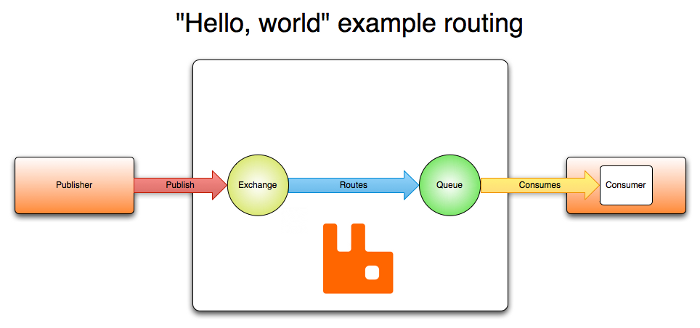
\includegraphics{assets/figures/rabbitmq.png}
    }
    \caption[\gls{AMQP} 0.9.1 Protocol Concepts]{\gls{AMQP} 0.9.1 Protocol Concepts by \cite{rabbitmqexpl}}
    \label{fig:implementation:decisions:rabbitmq}
\end{figure}

As discussed in \citetitle{rabbitmqexpl}, there are four types of exchanges:

\begin{itemize}
    \item Direct Exchange: ideal for the unicast routing of messages;
    \item Fanout Exchange: ideal for the broadcast routing of messages;
    \item Topic Exchange: ideal for the multicast routing of messages, queues subscribe to specific routing keys;
    \item Header Exchange: ideal for more flexible unicast routing of messages, queues subscribe to specific message headers.
\end{itemize}

This is the "core" protocol supported by the system.

The \gls{MQTT} protocol is a ``binary protocol emphasizing lightweight publish / subscribe messaging, targeted towards clients in constrained devices'' \parencite{rabbitmq}. According to \cite{mqtt}, this is the standard protocol for \gls{IoT} Messaging.

\cite{mqtt-vs-amqp} mentions that ``\gls{MQTT} has just one routing mechanism - topic subscriptions'', when compared with \gls{AMQP}. It can be seen as simpler version of \gls{AMQP} tailored for \gls{IoT} low powered devices. It has a lower message overhead, and instead of using \textit{'.'} as the level separator it uses a \textit{'/'}, for wildcards it uses \textit{'+'} instead of \textit{'*'}. 

Both protocols have various robust client libraries written for various programing languages \parencite{rabbitmq}. 

According to \cite{10.1145/3093742.3093908} the unique features of RabbitMQ are: (i) Standardized Protocol, (ii) Multi-protocol, (iii) Distributed Topology Modes, (iv) Comprehensive Management and Monitoring Tools, (v) Multi-tenancy and Isolation, (vi) Consumer Tracking, (vii) Disk-less Use, (viii) Publisher Flow Control, (ix) Queue Size Limits and (x) Message time to live.

\paragraph{Kafka}
\label{par:stateofart:arch:infra:mediator:kafka}

\citetitle{kafka} is a distributed event streaming platform that can be seen as an append-only-log. Its main concepts are: (i) events, (ii) producers, (iii) consumers and (iv) topics.

Events are sent by producers to specific topics that are partitioned by several Kafka brokers. Events are persisted, something that the \gls{AMQP} protocol doesn't do, and consumers can pull events from their subscribed topics. Since events are stored, a consumer can deliberately rewind back to an old offset and re-consume data \parencite{pubsubpushpull}. This enables consumers to easily follow the \citetitleyear{eventsourcing} and reconstruct an entity's current state by replaying the events.

``The Kafka ecosystem offers libraries and tools that provide additional functionality on top of Kafka'' \parencite{10.1145/3093742.3093908}, such as Kafka Connect and Kafka Streams.

According to \cite{kafkaconnect}, ``Kafka Connect works as a centralized data hub for simple data integration between databases, key-value stores, search indexes, and file systems''.

Kafka Streams ``is a client library for building applications and microservices, where the input and output data are stored in an Apache Kafka cluster. It combines the simplicity of writing and deploying standard Java and Scala applications on the client side with the benefits of Kafka's server-side cluster technology'' \parencite{kafkastreams}.

According to \cite{10.1145/3093742.3093908} the unique features of Kafka are: (i) Long term message storage, (ii) message replay, (iii) kafka connect and (iv) log compaction.

\subsubsection{IoT Middleware}
\label{subsubsec:stateofart:arch:infra:middleware}

The term \gls{IoT} Middleware in this work referes to platforms/solutions that offer or focus on three main features:

\begin{itemize}
    \item Device Management: device onboarding, maintenance, updates and monitoring;
    \item Data Transmission: device data collection and provision in real-time;
    \item Device Control: offer an \gls{API} to send commands to devices. 
\end{itemize}

These platforms handle the lower-layers communication protocols such as: (i) RFID, (ii) Bluetooth/BLE, (iii) LoRa and LoRaWAN, (iv) SigFox, (v) ZigBee, (vi) Thread, (vii) EnOcean, (viii) ANT, (ix) GPRS/2G/3G/4G/5G cellular, (x) Wi-Fi \parencite{DIAS2022100529}.

The article \citetitleyear{DIAS2022100529} argues that due to a lack of standards a designer can't objectively choose from one or another protocol when developing \gls{IoT} Systems. These platforms have the benefit of abstracting these lower-layers communication details and provide \gls{API}s that provision all data gathered with high-layer communication protocols like (i) HTTP, (ii) \gls{MQTT}, (iii) \gls{AMQP}, (iv) CoAP, (v) XMPP, (vi) LwM2M, (vii) LLAP, (viii) UPnP \parencite{DIAS2022100529}.

The platforms that will be briefly mentioned are:

\begin{itemize}
    \item \nameref{par:stateofart:arch:infra:middleware:ttn};
    \item \nameref{par:stateofart:arch:infra:middleware:azure};
    \item \nameref{par:stateofart:arch:infra:middleware:helium}.
\end{itemize}

This project focus mostly on \nameref{par:stateofart:arch:infra:middleware:helium} since it controls the lower-layers communication with the company's installed devices (via the community's installed hotspots).

\paragraph{The Things Stack}
\label{par:stateofart:arch:infra:middleware:ttn}

\citetitleyear{ttn} is behind the creation of a platform that focus on interacting with devices via LoRa and LoRaWAN.

Apart from the common features referred above, their cloud platform provides integrations with AWS IoT, Azure IoT Hub and other platforms such as Cumulocity, ThingsBoard, and LoRa Cloud. It also provides agnostic \gls{API}s based on \gls{MQTT}, webhooks and PubSubs to connect with other systems and publish the gathered device measures.

The company maintains an open-source version of their platform. According to \citetitleyear{ttn-stack}, this platform supports: almost all the LoRaWAN protocols specifications, device classes, regional parameters and onboarding options; device payload conversion for well-known formats or via custom Javascript functions; user and entity management; and GRPC and HTTP management \gls{API}s. 

\paragraph{Azure IoT Hub}
\label{par:stateofart:arch:infra:middleware:azure}

\citetitleyear{azure-hub} is a platform provided by Microsoft ``that acts as a central message hub for communication between an IoT application and its attached devices'' \parencite{azure-hub}. A helper service, Azure IoT Hub Device Provisioning Service, handles the registration and provisioning of devices.

According to \cite{azure-hub} data can also be routed to different services for further processing, it is possible to route data to: azure storage containers, event hubs, service bus queues and services bus topics. According to \cite{azure-hub-amqp}, it is also possible to subscribe to an \gls{AMQP} endpoint to receive the device measures sent to \gls{IoT} Hub. Azure IoT Hub also integrates with Azure Event Grid that allows one to register an HTTP endpoint for Azure Event Grid to dispatch events to, in this case, device measures.

According to \citetitleyear{azure-gartner}, Azure is a leading \gls{IoT} Platform.

\paragraph{Helium Console}
\label{par:stateofart:arch:infra:middleware:helium}

\citetitleyear{helium} is a new \gls{IoT} Platform. This platform's business model is fairly different from the ones mentioned before. Besides the platform itself, the company also maintains an open-source blockchain designed to power \gls{IoT} devices with wireless connectivity. Helium technology enables communication between devices and the internet by promoting the expansion of a new network operated by common people.

According to \cite{helium-wp}, `` Powering the Helium network is a blockchain with a native protocol token incentivizing a two-sided marketplace between coverage providers and coverage consumers''. Coverage providers install in their homes an \gls{IoT} gateway, Hotspot, that provides wide-area LoRaWAN coverage to the area surrounding it. Coverage consumers, e.g. \gls{IoT} devices, connect to this LoRaWAN network and send the gathered measures to the Hotspot. The Hotspot them routes the measures to the cloud in exchange for a transport fee, paid by the owner of the \gls{IoT} device.
The fee corresponds to a token that can be traded for dollars, bitcoin or any other available commodity on online exchanges.

In theory, this creates a self sustained economy that can provide to everyone a cheap and open communication layer for \gls{IoT} devices that is backed by open standards, and, provide a consistent income to those who what to support the network. The \textit{Helium Explorer Page}\footnote{\href {https://explorer.helium.com/}{link to Helium Explorer Page}} documents the number and location of each Hotspot, current there are almost a million of \gls{IoT} gateways installed throughout the world. Europe, USA and China are the regions with better network coverage.

This network, as an example, gives local farmers in remote locations the possibility to install a smart irrigation system without paying excruciating fees to an \gls{ISP} for satellite or 4G coverage.

The company's business idea is to utilize this low-cost network to offer \gls{IoT}-based services to small-to-medium size organizations.
Therefore, the solution to develop in this project will, at least in the near future, focus on the \gls{IoT} Middleware solution provided by Helium.

Helium Console enables devices to connect to pre-configured, cloud-based applications or send data directly over HTTP or MQTT via Integrations.
It currently supports two core integrations, HTTP and \gls{MQTT}, and multiple community integrations such as: (i) Helium Cargo, (ii) myDevices Cayenne, (iii) AWS IoT Core, (iv) Azure IoT Hub, (v) Azure IoT Central, (vi) Adafruit IO, (vii) Akenza, (viii) Datacake, (ix) Google Sheets, (x) Microshare, (xi) TagoIO, (xii) Ubidots \parencite{helium-integrations}. 

\subsubsection{Data Storage}
\label{subsubsec:stateofart:arch:infra:store}

This section refers to how information is stored and managed across systems.

A \gls{DBMS} is a general-purpose software system that facilitates the processes of defining, constructing, manipulating, and sharing data - \citetitle{elmasri2000fundamentals}. \gls{DBMS}s can be categorized according to several criteria, such as the data model, number of users or distribution. This section focus on the data model.

These are some of the data model types, according to \cite{elmasri2000fundamentals}:

\begin{itemize}
    \item The \textbf{relational data model} represents a database as a collection of tables, where each table can be stored as a separate file;
    \item The \textbf{document-based data model} is based on JSON (Java Script Object Notation) and stores the data as documents, which somewhat resemble complex objects;
    \item The \textbf{column-based data model} stores the columns of rows clustered on disk pages for fast access and allow multiple versions of the data;
    \item The \textbf{graph-based data model} stores objects as graph nodes and relationships among objects as directed graph edges;
    \item The \textbf{key-value data model} associates a unique key with each value (which can be a record or object) and provides very fast access to a value given its key.
\end{itemize}

The following sections briefly discuss these data models.

\paragraph{Relational Data Model}
\label{par:stateofart:arch:infra:store:relational}

This data model has a wide variety of usage in the industry. It relies on a ``schema to define exactly and unambiguously all the relationships of interest to the users'' \parencite{zaniolo1981design}. Therefore, it excels to represent concrete concepts within a business domain. According to \cite{jatana2012survey} almost all relational databases use \gls{SQL} to access and modify the data stored in the database. ``\gls{SQL} consists of a set of facilities for defining, accessing and otherwise managing data'' \parencite{date1989guide}. The reliability of a database model is checked with the help of ACID properties: \textbf{A}tomicity, \textbf{C}onsistency, \textbf{I}solation, \textbf{D}urability.

Some of the technologies that follow this data model are: (i) \citetitle{mysql}, (ii) \citetitle{postgressql} and (iii) \citetitle{oracledb}.
These are all ACID compliant and follow the SQL standard.

According to \cite{jatana2012survey}, this type of databases do not support high scalability, 
This data model is intended for strictly structured data with well defined interrelations.

\subsubsection{Document-based Data Model}
\label{par:stateofart:arch:infra:store:nosql}

This data model rose from the increasing need to store and analyze unstructured data as stated by \cite{miloslavskaya2016big}.  Citing \cite{elmasri2000fundamentals}, a ``major difference between document-based systems versus object and object-relational systems (relational database systems) is that there is no requirement to specify a schema''.

This data model, and all other mentioned below have some key differences when compared with the \nameref{par:stateofart:arch:infra:store:relational}.
Databases with this data model usually don't adder to the \gls{SQL} standard since there is no define notion of the data structure. Instead they follow the BASE acronym: \textbf{B}asically \textbf{A}vailable, \textbf{S}oft State and \textbf{E}ventually Consistent.

Some of the technologies that follow this data model are: \citetitle{mongodb} and \citetitle{firestore}.

\citetitle{mongodb} is open source and has a ``flexible document data model along with support for ad-hoc queries, secondary indexing, and real-time aggregations to provide powerful ways to access and analyze data'' \parencite{mongodb}.
Contrary to the \citetitle{mongodb}, \citetitle{firestore} is a close source service provided by google.

\subsubsection{Column-based Data Model}
\label{par:stateofart:arch:infra:store:time}

This data model is used in applications that require large amounts of data storage, and is commonly named \textit{data warehouses}. According to \cite{dehdouh2015using}, a data warehouse  is ``designed according to a dimensional modelling which has for objective to observe facts through measures, also called indicators, according to the dimensions that represent the analysis axes''. Citing \cite{han2011survey}, these databases ``can maintain high-performance of data analysis and business intelligence processing''.

Some of the technologies related to this concept are: (i) \citetitle{hbase}, (ii) \citetitle{cassandradb}, (iii) \citetitle{influxdb}, (iv) \citetitle{questdb}.

According to \cite{george2011hbase} HBase is a ``distributed, persistent, strictly consistent storage system with near-optimal write and excellent read performance''. This database uses \gls{HDFS} as its file system, and so, it is built on top of Hadoop.
HBase does not support a structured query language like \gls{SQL}, ``even though it's comprised of a set of standard tables with rows and columns, much like a traditional database'' \parencite{ibm-hbase}.

CassandraDB is a distributed storage system for managing very large amounts of structured data spread out across many commodity servers, while providing highly available service with no single point of failure \parencite{lakshman2010cassandra}.
It was developed internally by Facebook and then later open-sourced to the Apache Foundation. It doesn't support \gls{SQL}.

According to \cite{naqvi2017time}, InfluxDB is an ``open-source schemaless \gls{TSDB} with optional closed-sourced components developed by InfluxData. It is written in Go programming language and it is optimized to handle time series data.'' It provides an SQL-like query language and also defines a new protocol for fast data ingestion \parencite{ilp}.

QuestDB is a relational column-oriented database designed for time series and event data and entitles it self as the ``fastest open source time series database'' \parencite{questdb}.
According to benchmarks \parencite{quest-bench} preformed using the \gls{TSBS}, \cite{TSBS}, QuestDB ranks as the fastest option in the market.
It has out-of-the-box support for SQL Postgres wire protocol, (thus integrating with \citetitle{postgressql} client libraries), can be easily deployed using a single Docker Image, and also supports the \gls{ILP}.

\subsubsection{Graph-based Data Model}
\label{par:stateofart:arch:infra:store:graph}

According to \cite{angles2008survey}, the databases that follow this data model can be characterized as:

\begin{itemize}
    \item ``Data and/or the schema are represented by graphs, or by data structures generalizing the notion of graph (hypergraphs or hypernodes)'';
    \item ``Data manipulation is expressed by graph transformations, or by operations whose main primitives are on graph features like paths, neighborhoods, subgraphs, graph patterns, connectivity, and graph statistics'';
    \item ``Integrity constraints enforce data consistency. These constraints can be grouped in schema-instance consistency, identity and referential integrity, and functional and inclusion dependencies''.
\end{itemize}

These databases flourish when the importance of the information relies on the relations more or equal than on the entities, e.g. biology, Web mining and semantic Web, social networking and recommendation engines \parencite{angles2012comparison, miller2013graph}.

Some of the technologies related to this concept are: (i) \citetitle{neo4j}, (ii) \citetitle{dgraph}.

\subsubsection{Key-Value Data Model}
\label{par:stateofart:arch:infra:store:key}

Databases that follow this data model have their data represented as simple key and value relations. Citing \cite{pokorny2011nosql}, ``A key uniquely identifies a value (typically string, but also a pointer, where the value is stored) and this value can be structured or completely unstructured (typically BLOB). The approach key-value reminds simple abstractions as file systems or hash tables (DHT), which enables efficient lookups''.

Some of the technologies related to this concept are: (i) \citetitle{dynamodb}, (ii) \citetitle{redis}.

According to \cite{decandia2007dynamo} `` Dynamo has a simple key/value interface, is highly available with a clearly defined consistency window, is efficient in its resource usage, and has a simple scale out scheme to address growth in data set size or request rates''.

When compared with \citetitle{dynamodb}, \citetitle{redis} has a must more compelling feature, its license. \citetitle{redis} is an ``open source, in-memory data store used by millions of developers as a database, cache, streaming engine, and message broker'' \parencite{redis}.

\subsubsection{Rule Engine}
\label{subsubsec:stateofart:arch:infra:rule}

\subsection{Platforms}
\label{subsec:stateofart:arch:platforms}

Things Board

TagoIO

DataCake

Node-red

\subsection{Solutions}
\label{subsec:stateofart:arch:solutions}

This section focus on several solutions devoted to specific business cases.
The objective of this section is to simply introduce the major features of the solutions, how they work and what is the business model behind their company, when applicable.

The business cases addressed here are the ones this project attempts to answer.

\subsubsection{Indoor Fire Detention}
\label{subsubsec:stateofart:arch:solutions:fire}

\subsubsection{Smart Irrigation}
\label{subsubsec:stateofart:arch:solutions:irrigation}

This section mentions some Smart Irrigation Solutions discussed by \cite{OBAIDEEN2022100124}.

According to \cite{8372905} a Smart Irrigation System offers the following benefits: (i) Community Farming, (ii) Safety Control and Fraud Prevention, (iii) Competitive Advantages, (iv) Wealth Creation and Distributions, (v) Cost Reduction and Wastage, (vi) Operational Efficiency, (vii) Awareness and (ix) Asset Management.

As for the solutions:

WaterBit provides a ``secured wireless connectivity to its autonomous irrigation solution, allowing management and control of local irrigation'' \parencite{OBAIDEEN2022100124}. WaterBit gathers soil moisture levels measured every few minutes and presents theses measures via a mobile-friendly application where farmers can control the irrigation system.

Ipswich city council ``depicted that using an automated soil-moisture monitoring system as a driver of irrigation leads to significantly conserve water along with saving costs'' \parencite{OBAIDEEN2022100124}. The system's method to control the irrigation system was considered highly efficient when compared with a rainfall-based allocation method.

Maejo University in Thailand built a system to control the environment where mushrooms were cultivated. The system measured light, air temperature, air humidity and air flow to determine when to activate the irrigation system \parencite{OBAIDEEN2022100124}. The system was powered by solar energy.

AgirSens is a dynamic irrigation scheduling system based on IoT for efficient water management of irrigated crop fields. According to \cite{9249427} ``AgriSens has a farmer-friendly user interface, which provides field information to the farmers in a multimodal manner - visual display, cell phone, and Web portal''.

\subsubsection{Fleet Management}
\label{subsubsec:stateofart:arch:solutions:fleet}

This section focus on some Fleet Management and Asset Tracking solutions. No relevant papers were found regarding the use of \gls{IoT} in Fleet Management or Asset Tracking solutions, therefore the solutions here presented were gathered by the author based on the quality of information available regarding their company's business model, iot devices used and features offered.

As for the solutions:

Verizon Connect is a Fleet Management solution that provides it's own sensors/devices, platform and application under a subscription \parencite{verizon-iot}.
A team from Verizon installs the devices in the fleet according to the specification and access to the platform is given. This is an Hassle-free solution but the costs associated with it can be high. Since Verizon is a telecommunications conglomerate the protocols used to transport measures from devices to their platform is GPRS/2G/3G/4G/5G cellular.

SmartDrive is a Fleet Management solution that also provides it's own hardware, SR4, platform and application under a subscription. The SR4 is composed by a controller (solid-state storage, multiple communication protocols, advanced driver assistance system functions, computer-vision aided processing requirements), cameras, sensor bar (GPS, accelerometers, microphone and driver-support LEDs), keypad (for manual event recording and privacy mode initiation) and Wireless Key Fob (initiate a manual recording event, both inside and outside the vehicle) \parencite{smartdrive-iot}. With all the data gathered, their platform, Transportation Intelligence Platform, is capable of ``delivering breakthrough driving performance insights and analytic intelligence'', and ``helping fleets improve fleet safety and efficiency, and manage an entirely new set of business challenges arising in the future'' \parencite{smartdrive-iot2}.

LocaTrack is a platform for Asset Tracking built by Safecube \parencite{safecube}, this service provides the following Key Features: 

\begin{itemize}
    \item Geolocation: Distance, traveled road and availability;
    \item Asset use rate analysis: better visibility on the use of assets;
    \item Optimization: detailed analysis to optimize the use of assets;
    \item Real-time alert: real-time alerts on movements, geofencing, sleeping assets and others;
    \item Prediction: Maintenance, Servicing and Asset location;
    \item Condition monitoring: IoT trackers can detect changes in temperature, humidity or shocks and others.
\end{itemize}

According to \cite{safecube-azure}, LocaTrack uses SigFox for lower-level communication and Azure IoT Hub to collect the location of tracked assets.

Finally, TrackPac is a service for asset tracking \parencite{trackpac}. This service offers an application that presents real-time location data, battery data and geofence alerts of the managed assets. By using LoRaWAN (provided by Helium, the same network used in this project) for lower-level communication it promises a service ten times cheaper than the ones that require 4G. This service works with LoRaWAN class A trackers and does not enforce the use of any proprietary, close-source devices even though it recommends the use of Browan Tabs Object Locator, Digital Matter Oyster3 or Abeeway Micro. 

\subsection{Reference Architectures}
\label{subsec:stateofart:arch:ref}

As the \gls{IoT} domain covers such a wide spectrum of application fields with very little in common, the development cycles, technologies and architectures used can be completely different. The vast array of choices given to those involved in a greenfield project of this area, coupled with the lack of standards with a broad usage \parencite{DIAS2022100529, weyrich2015reference}, can linger the design, development and interoperability of \gls{IoT} systems.

Reference Architectures for the \gls{IoT} aim to help developers tackle some of these problems \parencite{weyrich2015reference}.

According to \cite{muller2008reference}, a Reference Architecture ``captures the essence of the architecture of a collection of systems. The purpose of a Reference Architecture is to provide guidance for the development of architectures for new versions of the system or extended systems and product families''.

This section sheds a light on some of the Reference Architectures of this field, what their focus is and the relevancy they have for this project.

The Reference Architectures discussed are: (i) \nameref{subsubsec:stateofart:arch:iota}, (ii) \nameref{subsubsec:stateofart:arch:sat}, (iii) \nameref{subsubsec:stateofart:arch:iira}, (iv) \nameref{subsubsec:stateofart:arch:wso2}, (v) \nameref{subsubsec:stateofart:arch:p2413}, (vi) \nameref{subsubsec:stateofart:arch:rami}, (vii) \nameref{subsubsec:stateofart:arch:azure}, (viii) \nameref{subsubsec:stateofart:arch:arrrowhead}.

This section was based on the papers written by \cite{Lynn2020} and \cite{DIAS2022100529}.

Intel System Architecture Specifications (Intel SAS) will not be discussed since no relevant information was found about it.
The \nameref{subsubsec:stateofart:arch:iota} also mentions the \gls{IoT} \gls{ARM}.

\subsubsection{IoT-A}
\label{subsubsec:stateofart:arch:iota}

The IoT Architecture goals are to create ``an architectural reference model for the interoperability of Internet-of-Things systems, outlining principles and guidelines for the technical design of its protocols, interfaces, and algorithms'' that shall ``lead to corresponding mechanism for its efficient integration into the service layer of the Future Internet''. \parencite{iot-a}. This project's final version is dated back to July 2013.

It defines a collection of Unified Requirements that support and validate concrete architectures created according to the \gls{IoT} \gls{ARM}. Some of these requirements were also applied to this project.

According to \cite{krvco2014designing}, this project motto is ``to offer IoT architects a common technical grounding in order to optimize interoperability. In that case, IoT applications would not be any longer built as stand-alone silo applications, but as inter-operable vertical applications still having a common "horizontal" grounding - the \gls{ARM} (compliant components, protocol suites, etc.)''.

This project originated the \gls{IoT} \gls{ARM} that can be divided into three interconnected parts \parencite{krvco2014designing}:

\begin{itemize}
    \item The IoT Reference Model;
    \item The IoT Reference Architecture;
    \item A set of Guidance (also called best practice).
\end{itemize}

The reference model defines several models that help to describe certain aspects of the \gls{IoT} architecture, some of this models are described by \cite{6682101}. It defines five core concepts:

\begin{itemize}
    \item Augmented Entity: a combination of a Physical Entity (real world object) and its Virtual Entity (digital representation);
    \item User: Those who interact with the system, human beings, devices, services and others;
    \item Device: Hardware to monitor or interact with real world objects;
    \item Resource: Computational element that gives access to information or control over a real-world object;
    \item Service: Entities that expose resources via a common interface, making then available for consumption by other services.
\end{itemize}

Each concept is them explored in detail. These concepts are them used to create the reference architecture.

According to \citetitleyear{iot-arm}, ``the Reference Architecture can be visualized as the "Matrix" that eventually gives birth ideally to all concrete architectures''. ``Guidance in form of best practices can be associated to a reference architecture in order to derive use-case-specific architectures from the reference architecture''.

The IoT Reference Architecture provides a functional view, presented in the Figure~\ref{fig:stateofart:arch:iota:functional}.

\begin{figure}[H]
    \centering
    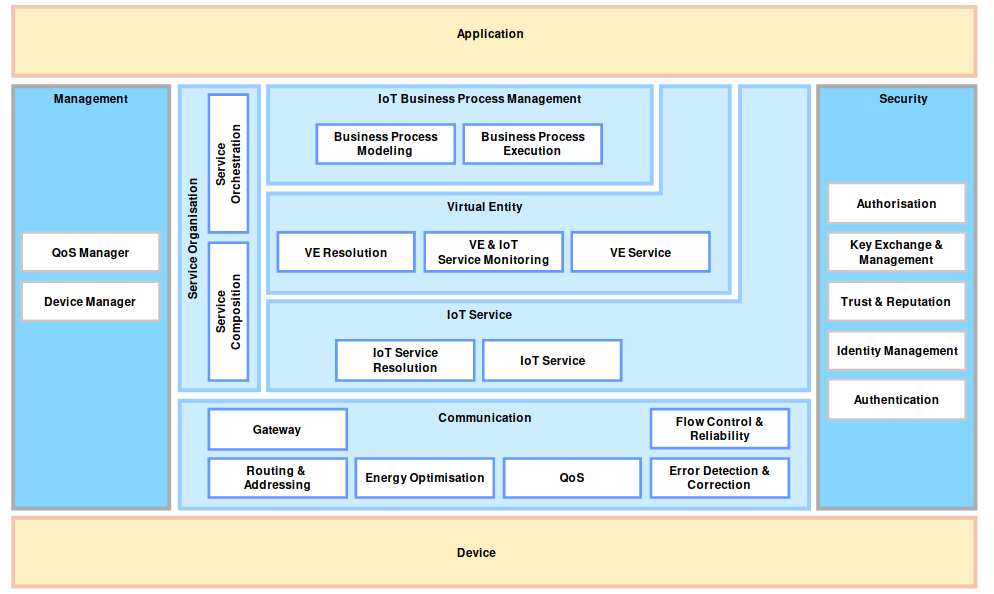
\includegraphics[scale=0.5]{
        assets/figures/arm-functional-view.png
    }
    \caption[ARM Functional View]{ARM Functional View, \cite{iot-arm-functional}}
    \label{fig:stateofart:arch:iota:functional}
\end{figure}

This functional view divides the architecture of a system in various functional components with well defined concerns.

\subsubsection{SAT-IoT}
\label{subsubsec:stateofart:arch:sat}

\cite{8767282} present an architectural model definition that lead to the development of ``a new advanced \gls{IoT} platform referred as SAT-IoT''. This model attempts to integrate concepts such as:  ``the paradigm of edge/cloud computing transparency, the IoT computing topology management, and the automation and integration of IoT visualization systems''. This project's final version is dated back to 2019, it apeares that the envisioned platform was not implemented since no other reference to it was found.

The diagram in Figure~\ref{fig:stateofart:arch:sat:model} defines the concepts, services and relations of this model.

\begin{figure}[H]
    \centering
    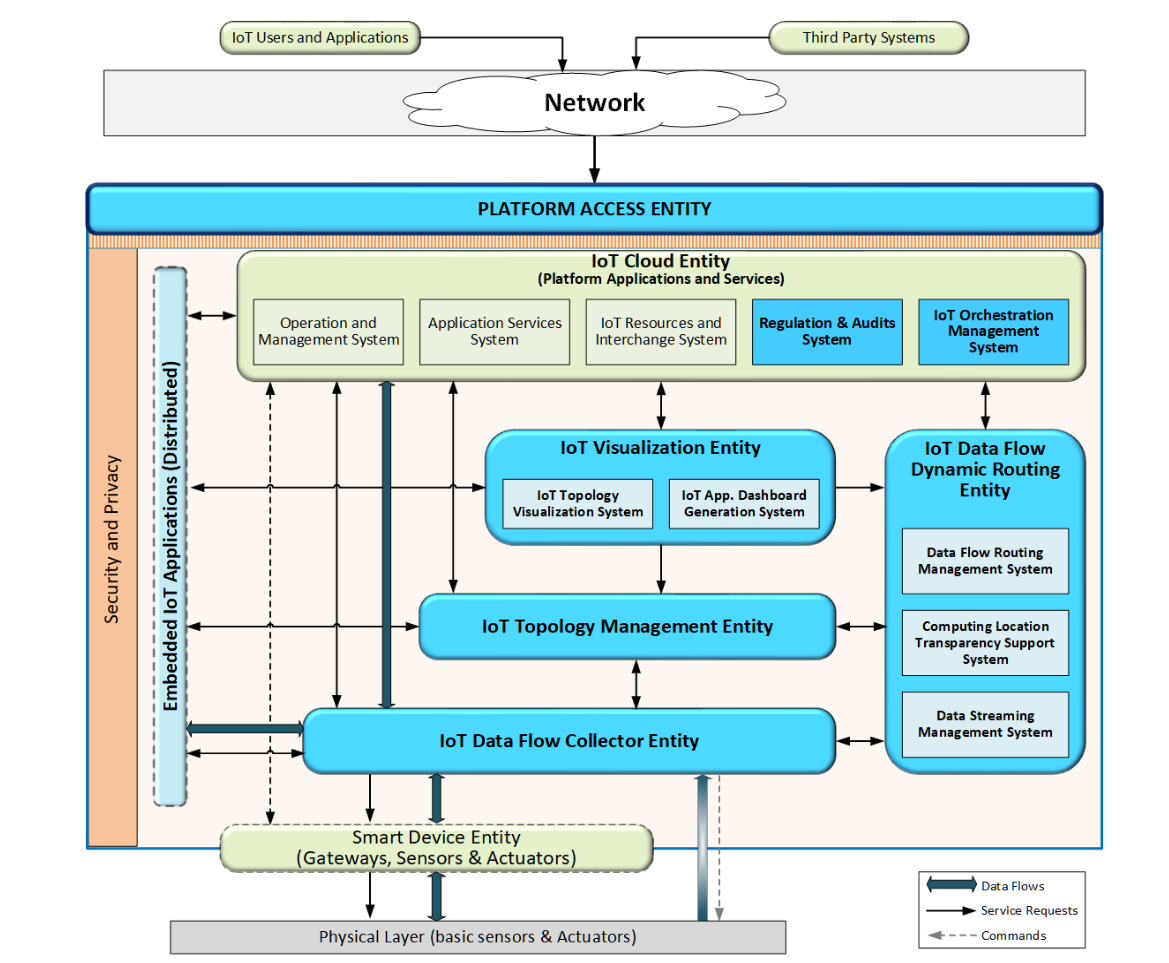
\includegraphics[scale=0.4]{
        assets/figures/sat-iot.png
    }
    \caption[SAT-IoT Architectural Model]{SAT-IoT Architectural Model, \cite{8767282}}
    \label{fig:stateofart:arch:sat:model}
\end{figure}

This model focus on a distributed system with a tree-like structure, where data can be dynamically processed in different node levels (edge, mid or cloud) in order to optimize response latency, bandwidth consumption, storage and other metrics. Components such as "IoT Topology Management Entity", "IoT Data Flow Dynamic Routing Entity" and "IoT Visualization Entity" focus on optimally distributing the workload across all nodes of the system.

The architecture also enables one to host "Embedded IoT Applications" that have full access to the system internals, leading to strongly integrated applications.

\subsubsection{IIRA}
\label{subsubsec:stateofart:arch:iira}

The \gls{IIRA} ``addresses the need for a common architecture framework to develop interoperable IIoT systems for diverse applications across a broad spectrum of industrial verticals in the public and private sectors to achieve the true promise of IIoT'' \parencite{iira}. This project's final version is dated back to June 2019.

It decomposes a typical Industrial \gls{IoT} system in five distinct functional domains:

\begin{itemize}
    \item \textbf{Control Domain}: this domain focus on functions that are performed by industrial control and automation systems. It is deployed in proximity to the physical systems and therefore geographically distributed;
    \item \textbf{Operations Domain}: this domain focus on the management and operation of the control domain. It should be able to configure, register, track and control assets. It is also responsible for providing real-time prognostics, monitoring and diagnostics of the managed assets;
    \item \textbf{Information Domain}: this domain is responsible for managing and processing data, it should transform, persist, and model or analyze data to acquire high-level intelligence about the overall system;
    \item \textbf{Application Domain}: this domain is responsible for applying business focused rules and logic to the gathered information;
    \item \textbf{Business Domain}: this domain is responsible for implementing business processes, such as Enterprise Resource Planning, Costumer Relationship Management, Manufacturing Execution System, Billing and Payment, Work Planning and Scheduling Systems. 
\end{itemize}

These domains interact according to Figure~\ref{fig:stateofart:arch:iira:domains}.

\begin{figure}[H]
    \centering
    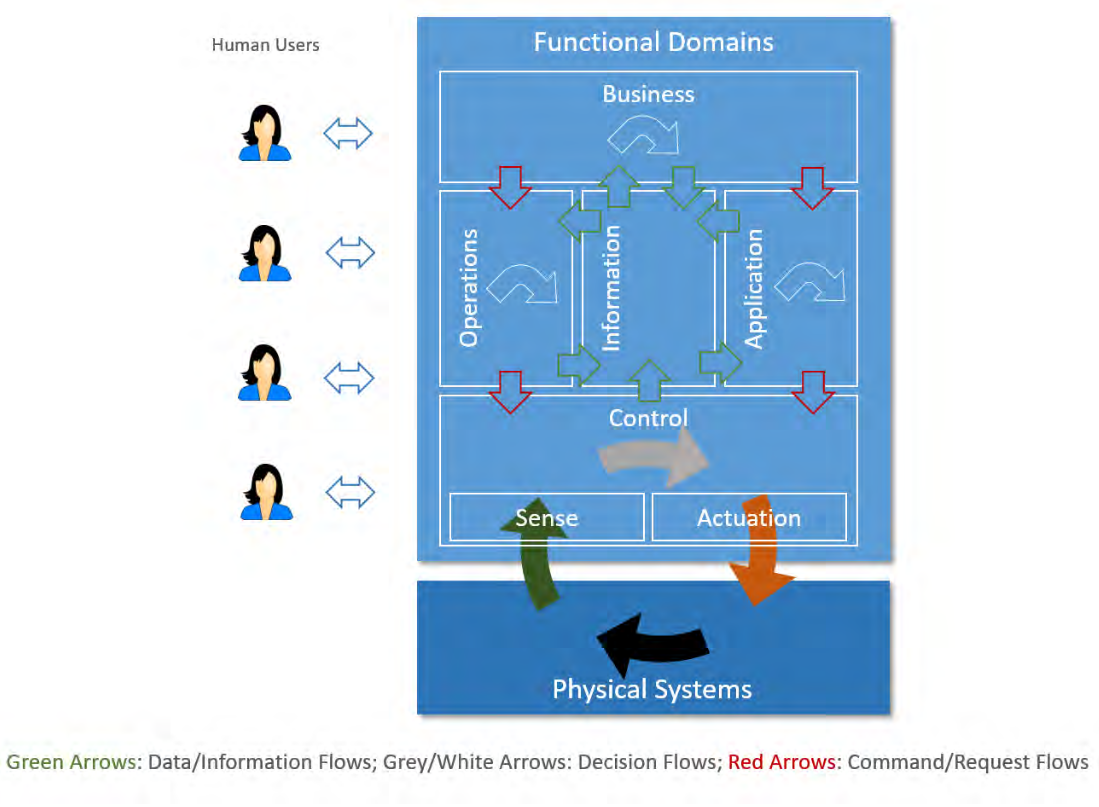
\includegraphics[scale=0.5]{
        assets/figures/irra-domains.png
    }
    \caption[\gls{IIRA} Functional Domains]{\gls{IIRA} Functional Domains, \cite{iira}}
    \label{fig:stateofart:arch:iira:domains}
\end{figure}

As information flows from the control domain to the business domain it is enriched, cleaned, filtered and combined leading to a broader and richer notion of the complete environment. New information can be derived, and new intelligence may emerge from this broader information.

When applied to the common three tier architecture for IoT systems, these domains are organized according to Figure~\ref{fig:stateofart:arch:iira:applied}.

\begin{figure}[H]
    \centering
    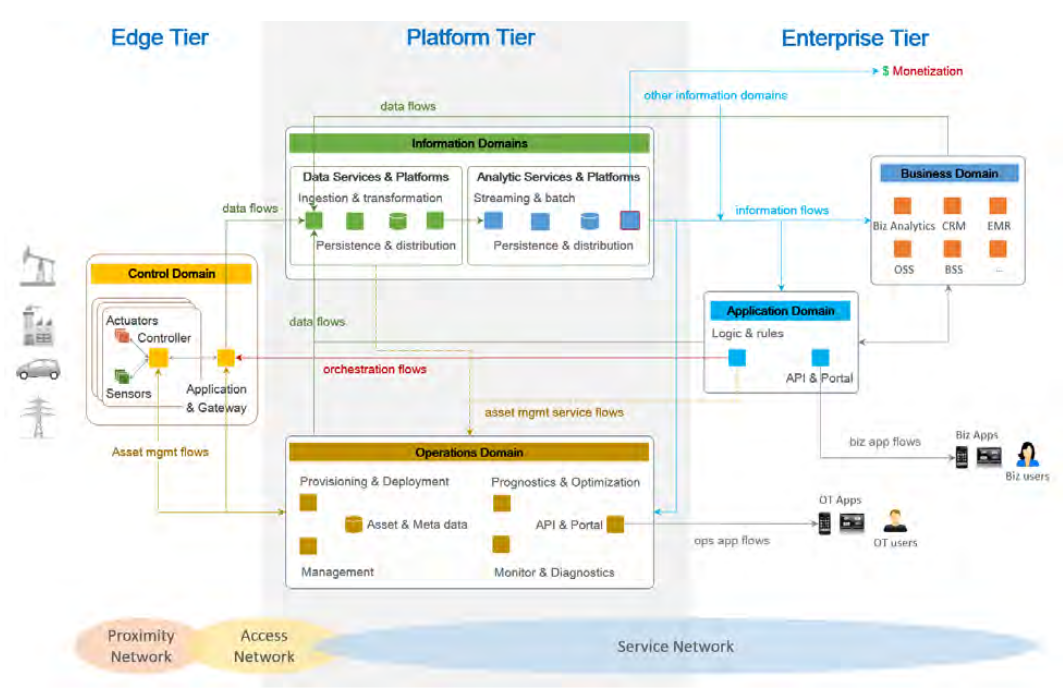
\includegraphics[scale=0.5]{
        assets/figures/irra-applied.png
    }
    \caption[Mapping between a three tier architecture and the \gls{IIRA} function domains]{Mapping between a three tier architecture and the \gls{IIRA} function domains, \cite{iira}}
    \label{fig:stateofart:arch:iira:applied}
\end{figure}

\subsubsection{WSO2 IRA}
\label{subsubsec:stateofart:arch:wso2}

The WSO2 reference architecture aims to ``provide an architecture that supports integration between systems and devices'' \parencite{wso2ira}. This project's final version is dated back to October 2015.

It groups the \gls{IoT} related requirements in the following key categories: (i) Connectivity and communications, (ii) Device management, (iii) Data collection, analysis, and actuation, (iv) Scalability, (v) Security, (vi) high-availability, (vii) Predictive analysis and (viii) Integration.

This categories gave birth to the following reference architecture, Figure~\ref{fig:stateofart:arch:wso2:ra}.

\begin{figure}[H]
    \centering
    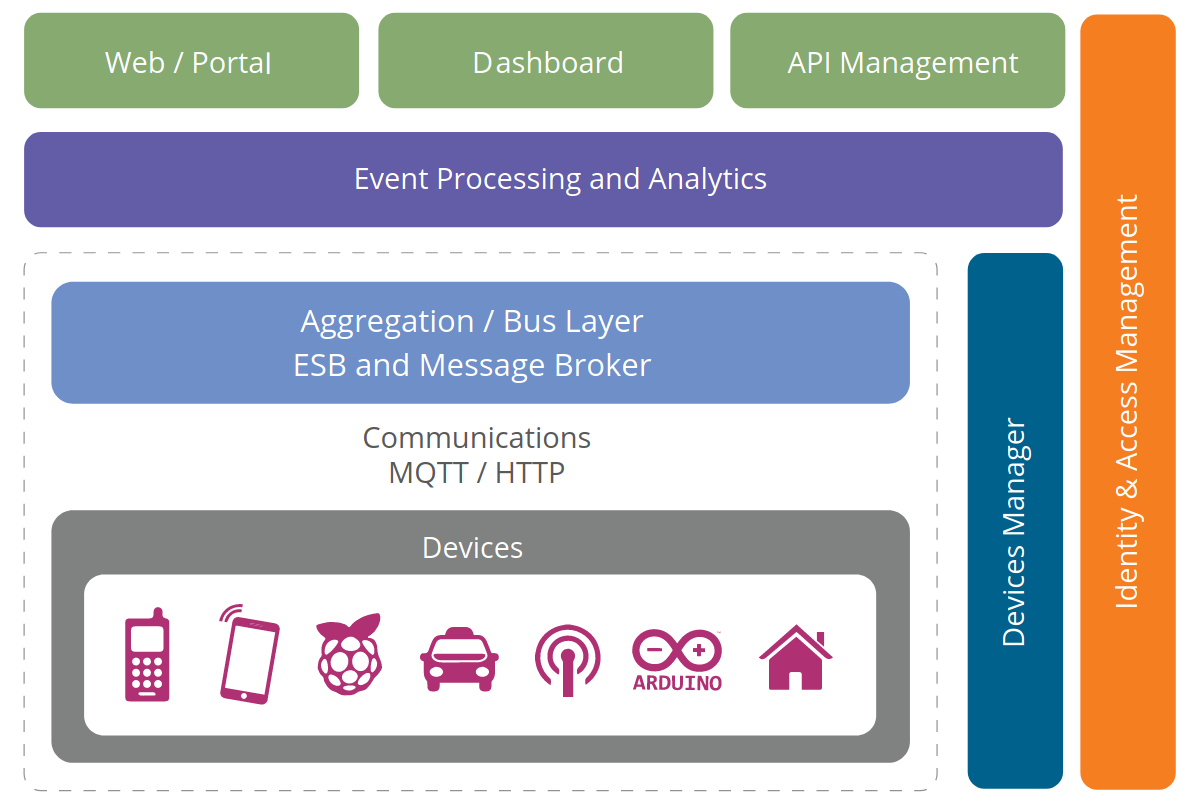
\includegraphics[scale=0.4]{
        assets/figures/wso2-ira.png
    }
    \caption[WSO2 Reference Architecture for IoT]{Reference Architecture for IoT, \cite{wso2ira}}
    \label{fig:stateofart:arch:wso2:ra}
\end{figure}

This reference architecture envisions two cross-cutting and five horizontal layers:

\begin{itemize}
    \item \textbf{Device Layer} (in grey): related to the physical \gls{IoT} devices;
    \item \textbf{Communications Layer} (without any representative color): related to the connectivity of devices;
    \item \textbf{Aggregation/bus Layer} (in light blue): related to the aggregation and supply of data upstream, bridging between the protocols used in upstream layers and downstream layers; 
    \item \textbf{Event processing and Analytics Layer} (in purple): related to data processing, analysis and storage;
    \item \textbf{Client/external Communications Layer} (in green): related to web-based frontends and portals that interact with the Event processing and Analytics layer, dashboards that
    offer views into analytics and event processing, and \gls{API}s for machine to machine communication;
    \item \textbf{Device Management Layer} (in dark blue): related to the management, onboarding and remote control of devices;
    \item \textbf{Identity Access Management} (in orange): related to the authentication and authorization of users and systems that interact with the system.
\end{itemize}

In the Event processing and analytics Layer it's recommended the use of ``a highly scalable, column-based data storage for storing events'', ``map-reduce for long-running batch-oriented processing of data'', ``complex event processing for fast in-memory processing and real-time reaction and autonomic actions based on the data an activity of devices and other systems'' and ``traditional application processing platforms'' (custom-made applications for data processing).

\subsubsection{IEEE P2413}
\label{subsubsec:stateofart:arch:p2413}

The IEEE Standard for an Architectural Framework for the IoT ``defines an architecture framework description for \gls{IoT}''. The architecture framework defined in the standard ``will promote cross-domain interaction, aid system
interoperability and functional compatibility, and further fuel the growth of the IoT market'' \parencite{9032420}.  This project's final version is dated back to June 2020.

Its architecture framework covers the definition of basic architectural building blocks and their ability to be integrated into multi-tiered systems. It describes different detailed viewpoints of the framework \parencite{9032420}:

\begin{itemize}
    \item \textbf{Conceptual Viewpoint}: concerned with defining a common vocabulary and semantics regarding a \gls{IoT} System to ease the communication across teams and encourage the reuse of concepts;
    \item \textbf{Compatibility Viewpoint}: concerned with the compatibility between systems and devices to lower the cost of integration. This viewpoint urges for the creation of new standards and compliance with those standards. It defines six levels of compatibility focused specially on physical devices: (i) incompatible, (ii) coexistent, (iii) inter connectable, (iv) inter workable, (v) interoperable and (vi) exchangeable;
    \item \textbf{Lifecycle Viewpoint}: concerned with a system's assurance, performance, maintainability and evolvability across its lifecycle: design, development, production, support, upgrade and retirement; 
    \item \textbf{Communication Viewpoint}: concerned with how devices can exchange information with each other and \gls{IoT} systems in a accurate, precise and effective manner;
    \item \textbf{Information Viewpoint}: concerned with how information is semantically defined, structured, stored, shared, manipulated, managed, and distributed across the IoT system. This viewpoint should focus on documenting system-level information, e.g., information exchanged between the various subsystems;
    \item \textbf{Function Viewpoint}: concerned with how devices can function according to their intended purpose or characteristic action, such as actuation, sensing, analysis, or control of entities of interest; 
    \item \textbf{Thread model Viewpoint}: concerned with identifying potential threats that could exploit vulnerabilities in the device, network or subsystems that encapsulate the \gls{IoT} system;
    \item \textbf{Security and safety monitoring Viewpoint}: concerned with monitoring the events occurring in an \gls{IoT} system and analyzing them for signs of possible incidents, which are violations or imminent threats of violation of security, safety, or acceptable use policies, or standard security practices;
    \item \textbf{Access control Viewpoint}: concerned with permitted activities of legitimate users, mediating every attempt by a user to access a resource in the IoT system. It is composed by three security functions: identification, authentication and authorization;
    \item \textbf{Privacy and trust Viewpoint}: concerned with the privacy of individuals or groups and trust in systems or organizations. In a complex \gls{IoT} system, arbitrary device data can be grouped and analyzed to determine the users activities;
    \item \textbf{Collaboration Viewpoint}: concerned with the collaboration of systems that belong to different application domains;
    \item \textbf{Computing resource Viewpoint}: concerned with the computing resources needed to support the \gls{IoT} system as a whole, such as gateways, data centers, \gls{PLC}s and \gls{DCS} controllers, microcontrollers embedded in sensors and actuators or others.
\end{itemize}

The idealized \gls{IoT} System should be examined according to these viewpoints in order to better define its architecture.

\cite{9032420} then procedes to define the Standard for a Reference Architecture for Smart Cities in P2413.1, the major focus of this project's business cases.

One of the architectures proposed in the standard and derived from the architecture framework is presented in Figure~\ref{fig:stateofart:arch:p2413:rasc}. 

\begin{figure}[H]
    \centering
    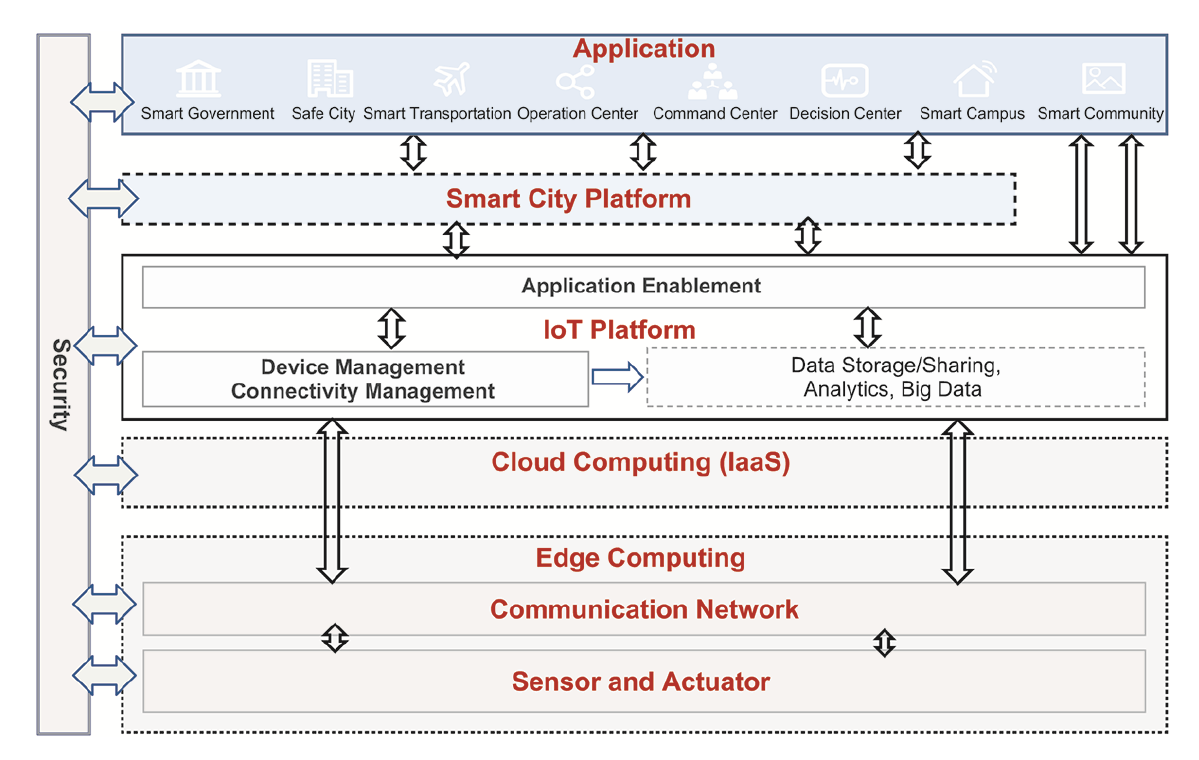
\includegraphics[scale=0.4]{
        assets/figures/smart-city-p2413.png
    }
    \caption[Example of an \gls{IoT} System Architecture for Smart Cities]{Example of an \gls{IoT} System Architecture for Smart Cities, \cite{9032420}}
    \label{fig:stateofart:arch:p2413:rasc}
\end{figure}

This architecture, derived from the common three tier architecture for \gls{IoT} Systems, proposes a new tier entitled Smart City Platform, in it ``Northbound APIs support diverse vertical applications development and southbound APIs connect to different IoT Platforms'' \parencite{9032420}.

\subsubsection{RAMI 4.0}
\label{subsubsec:stateofart:arch:rami}

The Reference Architectural Model Industry 4.0 ``ensures that all participants involved share a common perspective and develop a common understanding'' and is represented by a ``three-dimensional map showing the most important aspects of Industrie 4.0'' \parencite{hankel2015reference}. It represents a service-oriented architecture according to the manufactures association that defined it. This project's final version is dated back to August 2018 and has clear focus on the \gls{IoT} business area related to the Industry, e.g. smart factories.

The three-dimensional map is depicted in Figure~\ref{fig:stateofart:arch:rami:map}.

\begin{figure}[H]
    \centering
    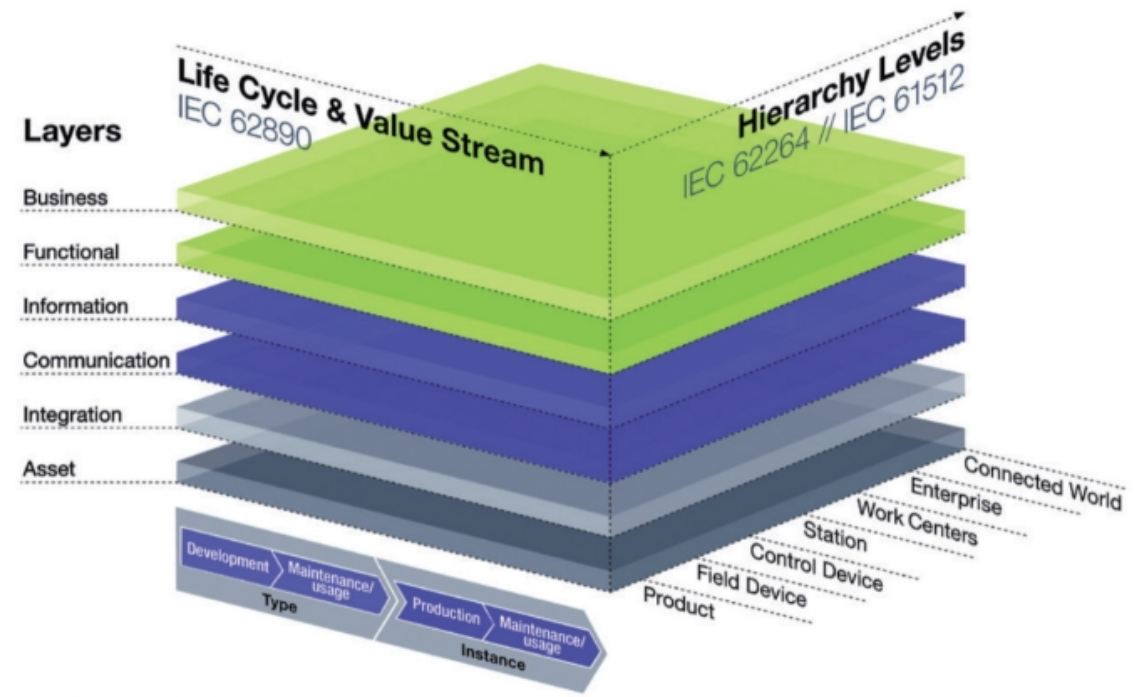
\includegraphics[scale=0.4]{
        assets/figures/rami.png
    }
    \caption[RAMI 4.0 Three-dimensional map]{RAMI 4.0 Three-dimensional map, \cite{rami}}
    \label{fig:stateofart:arch:rami:map}
\end{figure}

According to \cite{rami-explained} it is comprised of six architecture layers stretched across the hierarchy and life cycle axes:

\begin{itemize}
    \item \textbf{Business Layer}: concerned with Organization and Business processes;
    \item \textbf{Functional Layer}: concerned with the Functions of assets;
    \item \textbf{Information Layer}: concerned with the processing of the necessary data; 
    \item \textbf{Communication Layer}: concerned with how to gain access to the information needed;
    \item \textbf{Integration Layer}: concerned with the transition from things to the digital world;
    \item \textbf{Asset Layer}: concerned with the physical things in the real world.
\end{itemize}

This reference architecture mentions an administration shell that sits in between the asset (machine, sensor, unit or plant) and the network. This administration shell is the interface connecting the \gls{IoT} platform to the asset, storing all data and information about the asset and standardizing the network's communication. According to \cite{rami2}, ``each physical thing has its own administration shell'' and ``several assets can form a thematic unit with a common administration shell''. This administration shell allows for distributed data analysis and control over assets. 

According to \cite{iira-inter-rami}, this reference architecture is aligned with \nameref{subsubsec:stateofart:arch:iira}. The following picture, Figure~\ref{fig:stateofart:arch:rami:mapping} describes how RAMI 4.0 concepts can be represented according to IIRA.

\begin{figure}[H]
    \centering
    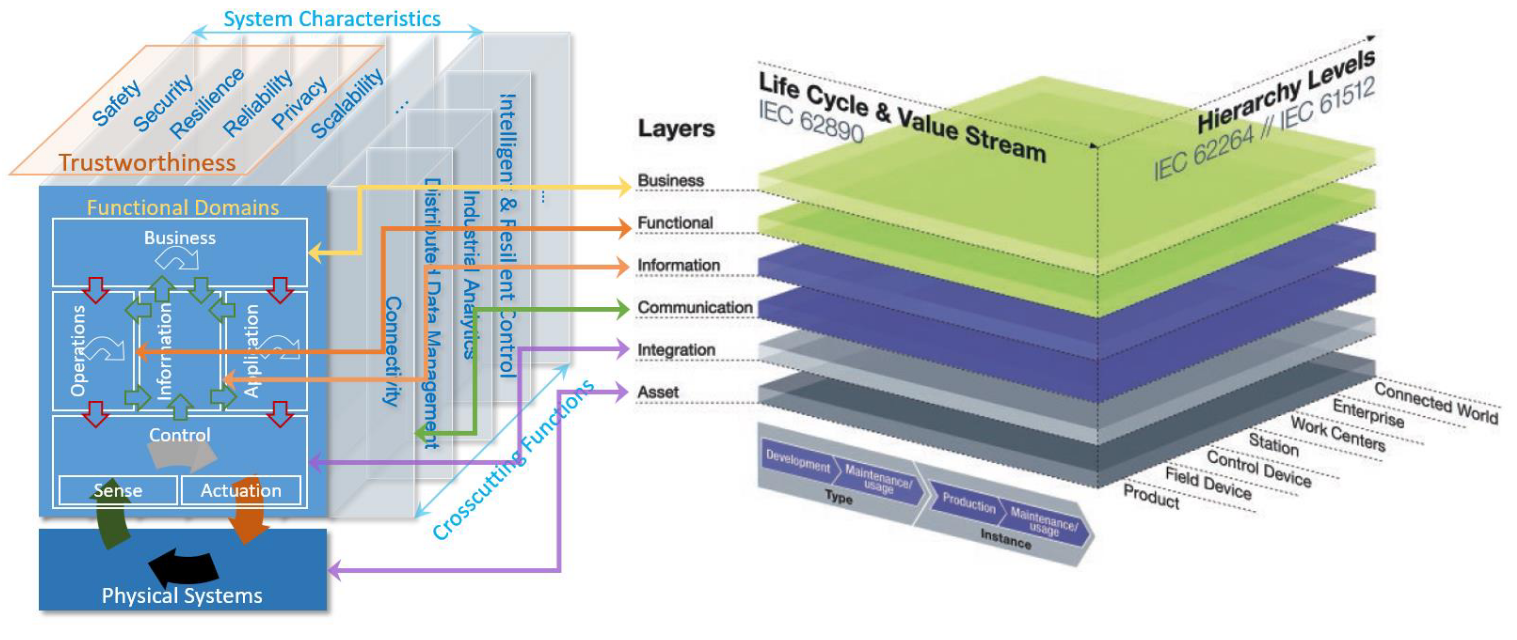
\includegraphics[scale=0.35]{
        assets/figures/iira-rami-mapping.png
    }
    \caption[IIRA and RAMI 4.0 Functional Mapping]{IRRA and RAMI 4.0 Functional Mapping, \cite{iira-inter-rami}}
    \label{fig:stateofart:arch:rami:mapping}
\end{figure}

The need to map the concepts of both reference architectures derives from the fact that these two are the most actively references used in the industry \parencite{DIAS2022100529}. Therefore, the document by \cite{iira-inter-rami} provides guidelines on how to achieve better interoperability between systems built according to different reference architecture. 

\subsubsection{Azure IRA}
\label{subsubsec:stateofart:arch:azure}

The \citetitleyear{azure-ira} proposes the architecture envisioned in Figure~\ref{fig:stateofart:arch:azure:ira}, this architecture relies heavily on the Azure platform services. According to \cite{azure-ira}, the recommended architecture is ``cloud native, microservice, and serverless-based''. This project's final version is dated back to April 2021.

\begin{figure}[H]
    \centering
    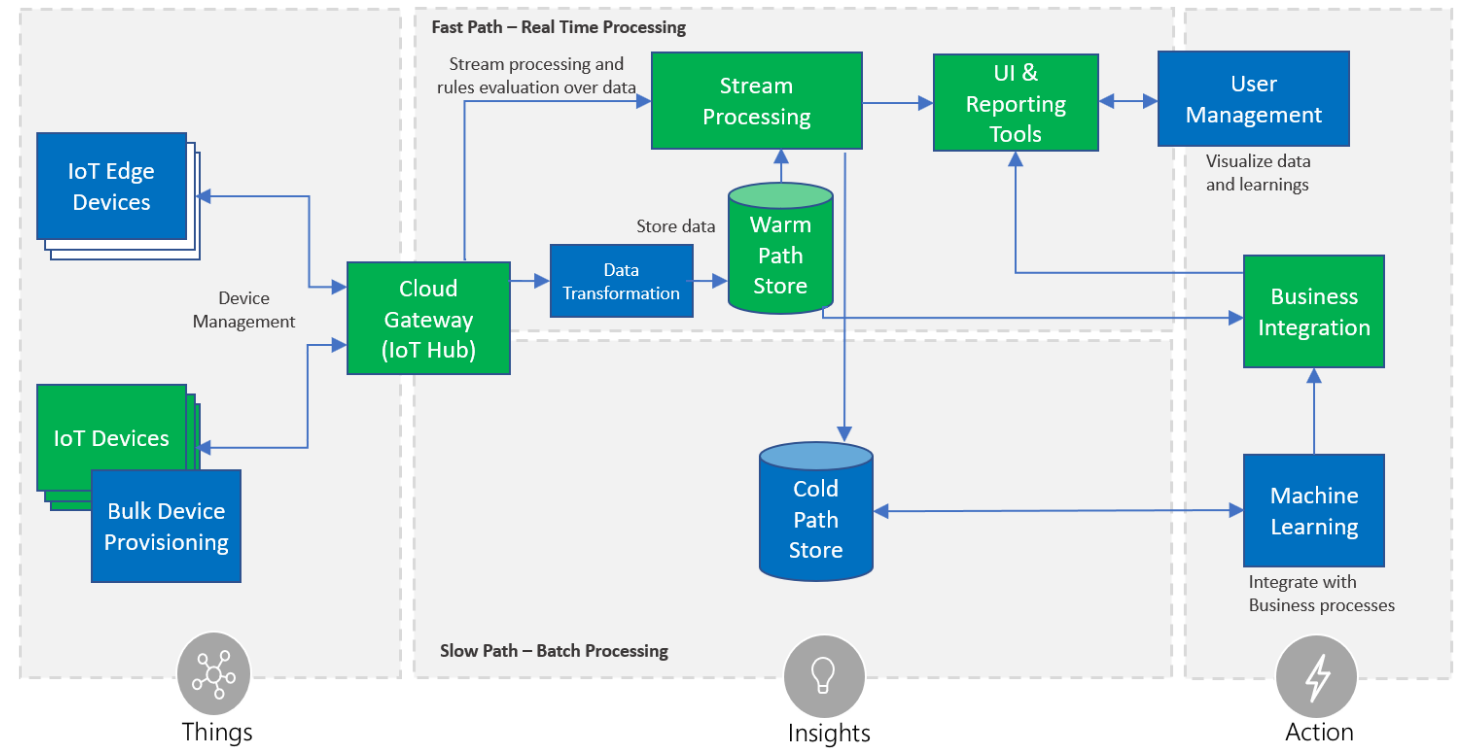
\includegraphics[scale=0.35]{
        assets/figures/azure.png
    }
    \caption[Azure IoT Reference Architecture]{Azure IoT Reference Architecture, \cite{azure-ira}}
    \label{fig:stateofart:arch:azure:ira}
\end{figure}

\cite{azure-ira} recommends that ``subsystems should be built as discrete services that are independently deployable, and able to scale independently'', to ``enable greater scale, more flexibility in updating individual subsystems, and provide the flexibility to choose appropriate technology on a per-subsystem basis''.

This reference architecture is based on the lambda architecture. According to \cite{kiran2015lambda}, the lambda architecture ``combines both batch and stream processing capabilities for online processing and handling of massive data volumes in a uniform manner, reducing costs in the process.''
It is comprised of three layers (or patches), a Batch or Slow layer for extensive and prolonged analysis, a Speed or Fast layer for real-time evident information, and a Serving layer responsible for providing the results gathered by the other two layers.

As we can see in Figure~\ref{fig:stateofart:arch:azure:ira} the Insights section is divided into two patches, the Fast Patch for real-time processing, and the Slow Patch for batch processing. Results are then provided in the Action section.

\subsubsection{Arrowhead}
\label{subsubsec:stateofart:arch:arrrowhead}

According to \cite{varga2017making}, ``the objective of the Arrowhead Framework is to efficiently support the development, deployment and operation of interconnected, cooperative systems. It is based on the \gls{SOA} philosophy''. It has a big focus on Interoperability between systems and services already in production.

``The Arrowhead project targets five business domains; Production (process and manufacturing), Smart Buildings and infrastructures, Electro mobility, Energy production and Virtual Markets of Energy'' \parencite{blomstedt2014arrowhead}.

The Arrowhead challenge is to enable interoperability between these systems, therefore, it starts by defining how one should document his/her solutions. Three hierarchical levels of solutions are proposed: (i) service, (ii) system, (iii) system of systems (Figure~\ref{fig:stateofart:arch:arrowhead:levels}).

\begin{figure}[H]
    \centering
    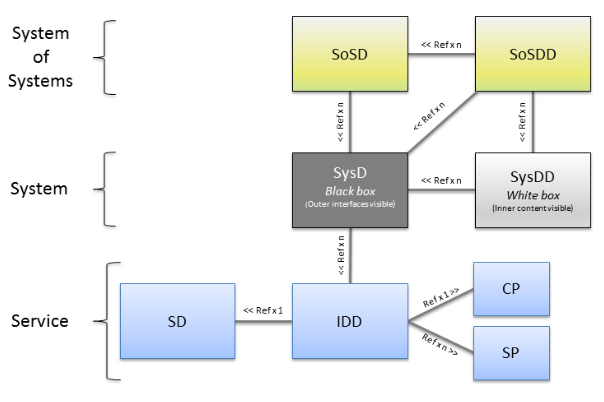
\includegraphics[scale=0.6]{
        assets/figures/arrowhead-levels.png
    }
    \caption[Arrowhead Framework Core and Application Services]{Arrowhead Framework Core and Application Services, \cite{blomstedt2014arrowhead}}
    \label{fig:stateofart:arch:arrowhead:levels}
\end{figure}

The lower level, service, can be something that, for example, indicates the current measured humidity level by sensor \textit{X} (pull-typed service) or that opens/closes valve \textit{Y} (push-typed service). A system is composed by several services. A System of Systems is composed by several systems that work in harmony in a Arrowhead local cloud. A Arrowhead local cloud is composed by at least three mandatory core systems: (i) ServiceRegistry system, (ii) Authorization system and (iii) Orchestration system presented in Figure~\ref{fig:stateofart:arch:arrowhead:system}.

\begin{figure}[H]
    \centering
    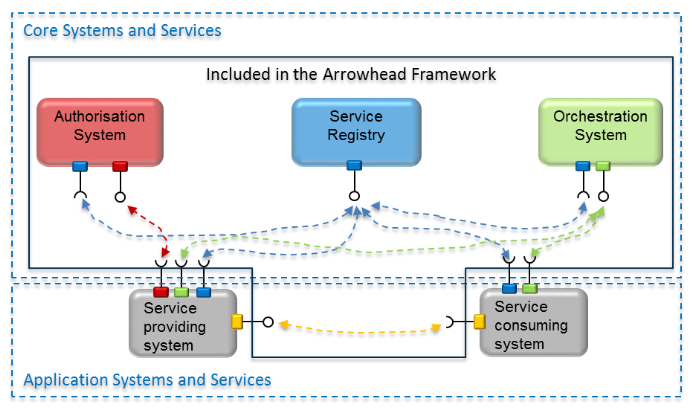
\includegraphics[scale=0.6]{
        assets/figures/arrowhead.png
    }
    \caption[Arrowhead Framework Core and Application Services]{Arrowhead Framework Core and Application Services, \cite{blomstedt2014arrowhead}}
    \label{fig:stateofart:arch:arrowhead:system}
\end{figure}

These core systems handle essential features for a local cloud such as: service discovery, service registration, service advertisement, authentication of consuming services, data exchange between systems and service coordination according to \cite{marcu2020arrowhead}. A local cloud can expose its systems to other local clouds and consume other local clouds systems. Since each service and system is well documented and arrowhead compliant it's possible to ensure interoperability between local clouds.

\subsubsection{Overall Perspective}
\label{subsec:stateofart:arch:prepective}

To close this section, some of the author sentiment and ideas surrounding these reference architecture models, and how they may shape this project's solution, are presented:

\begin{itemize}
    \item \nameref{subsubsec:stateofart:arch:iota}: The Unified Requirements detailed by this initiative gave the author an idea of the basic features for an \gls{IoT} system and enriched the requirements proposed by the company;
    \item \nameref{subsubsec:stateofart:arch:sat}: The extendability notion behind the "Embedded IoT Application" component was interesting to author from a business point of view. This idea would give customers the possibility to integrate custom-made solutions in the platform;
    \item \nameref{subsubsec:stateofart:arch:iira}: The author argues that the clear division between the Application, Information and Business domains provide a common abstraction that can be applied to any \gls{IoT} System to ease the cognitive burden taken to understand it;
    \item \nameref{subsubsec:stateofart:arch:wso2}: The author finds the clear division between the responsibilities of gathering measures, processing and analyzing them, and providing them in a business focused manner very aligned with this project's goals;
    \item \nameref{subsubsec:stateofart:arch:p2413}: The concept of "Smart City Platform", and how it interacts with various systems is highly related with the overall requirements of this project;
    \item \nameref{subsubsec:stateofart:arch:rami}: This reference architecture provided no relevant insight for the author, mostly due to the discrepancy between the \gls{IoT} domains each project was devoted to (Smart Cities vs Industry 4.0);
    \item \nameref{subsubsec:stateofart:arch:azure}: This reference architecture presented the author with a conceivable architecture for the future of the current solution. It introduced the notion of a Batch layer to better handle complex and prolonged analysis and provide \gls{KPI} reports;
    \item \nameref{subsubsec:stateofart:arch:arrrowhead}: This reference architecture appeared to be out-of-scope for the project since it focus on a more fine-grained access and control of devices (without the need for a \gls{IoT} Midlleware that handle device management and propagation of measures).
\end{itemize}

\subsection{Synopsis}
\label{subsec:stateofart:synopsis}

This section introduced the reader to the technological landscape of \gls{IoT}. The next section discusses some of its business areas or domains.

\section{Business Areas}
\label{sec:stateofart:areas}

Even though there's no concise structure, it is obvious that the \gls{IoT} technologies can be used in a broad range of areas/sectors. According to \cite{nivzetic2019smart}, the most valuable areas are: Smart Cities, Industrial \gls{IoT}, Connected Health and Smart Homes. The general market division of IoT technologies is presented in Figure~\ref{fig:iot-areas}.

\begin{figure}[H]
    \centering
    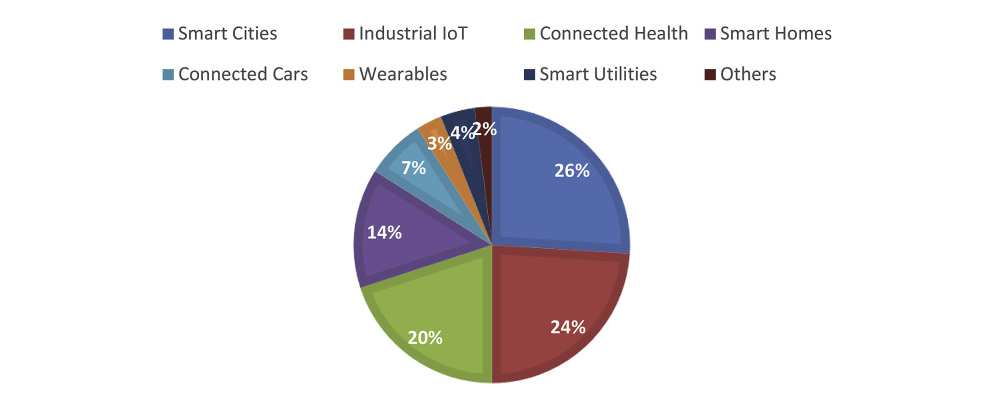
\includegraphics[scale=0.5]{
        assets/figures/iot-areas.png
    }
    \caption[IoT market structure]{General market structure of IoT technologies, \cite{nivzetic2019smart}}
    \label{fig:iot-areas}
\end{figure}

From another point of view, and according to \cite{7073822}, the sectors \gls{IoT} is related to are: Energy, Smart City, Transportation, Smart Home, Environment, Supply Chain, and Health Care.

According to (\cite{6851114}) these are the main application fields for \gls{IoT} in China: industry, smart agriculture, smart logistics, intelligent transportation, smart grids, smart environmental protection, smart safety, smart medical and smart home.

Even though this work focus mostly on Smart Cities other areas are also be described. Each of this areas incorporate several interconnected use cases that are briefly described in the following segments.

\subsection{Smart Cities}
\label{subsec:stateofart:areas:cities}

The Smart Cities sector includes numerous use cases related to public safety, the environment, mobility, energy, infrastructure and many other municipal concerns. According to \cite{iot-smart-city-prioritized} this are the use cases being prioritized.

\begin{itemize}
    \item Connected Public Transport: real-time monitoring of public transportation vehicles' locations, stops and itineraries, and the possibility to be notified when a public transportation vehicle is arriving at a stop;
    \item Traffic Monitoring and Management: real-time monitoring and management of traffic flows in a efficient manner;
    \item Water level / Flood Monitoring: real-time monitoring of level of water in public water basins such as rivers, channels, or even lakes and seas to warn and predict fast water level shifts;
    \item Video Surveillance \& Analytics: real-time monitoring using \gls{CCT} cameras and analytics to detect specific situations, e.g. accidents, crimes, potential threats, or recognize specific features (face recognition, demographics, etc.);
    \item Connected Streetlights: real-time monitoring and management of streetlights' health status and energy consumption to decrease costs and become more sustainable;
    \item Weather Monitoring: real-time monitoring of weather conditions such as temperature, humidity, rainfall, wind speed and direction to predict the weather and future natural disasters;
    \item Air Quality / Pollution Monitoring: real-time monitoring of air quality to warn the community about hazardous conditions;
    \item Smart Metering - Water: remote real-time monitoring of water usage in homes to address the world's water demand and scarcity issues and faster localize sewage leaks;
    \item Fire / Smoke Detention: real-time monitoring of possible indoor fires and CO2 levels to prevent injuries, fatalities and building degradation;
    \item Water Quality Monitoring: real-time monitoring of water conditions such as pH levels, percentage of salts and other elements that can threaten the public health.
\end{itemize}

Apart from these use cases, others are arising, such as smart parking (\cite{GOAP201841}), smart irrigation (\cite{7562735}) and waste management (\cite{7972276}).
\begin{itemize}
    \item Smart parking provides a simple method to the community of knowing the available parking spots, which, alone, lowers the carbon footprint and traffic congestions in cities.

    \item Smart irrigation tackles the need to save water by irrigating the soil only when needed and not when it is already moist, it's raining or it is expected to rain in the following hours.

    \item Waste management can eliminate the cost of unnecessary waste collections and therefore reduce the carbon footprint. Data gathered can then help to identifying cost-effective itineraries to collect waste and eventually lower overall transportation and staff costs.
\end{itemize}

All this use cases refine the efficiency of the municipal workforce and help the town council to reduce costs and improve the environment sustainability in the long term.

\subsection{Industry}
\label{subsec:stateofart:areas:industry}

According to \cite{iiot}, ``the Industrial \gls{IoT} provides a way to get better visibility and insight into the company's operations and assets", therefore this leads to ``operational efficiency gains and accelerated productivity, which results in reduced unplanned downtime and optimized efficiency, and thereby profits"".
It is comprised of several use cases (\cite{iiot-cases}) such as:

\begin{itemize}
    \item Predictive Maintenance: real-time monitoring of equipment conditions and applied data analytics can help a company to significantly decrease operational expenditures. ``Other potential advantages include increased equipment lifetime, increased plant safety and fewer accidents with negative environmental impact"" (\cite{iiot-cases});
    \item Smart metering: real-time monitoring of energy, water or natural gas consumption of a building can reduce operating expenses by managing manual operations remotely, reduce energy theft and improve forecasting and streamline power-consumption (\cite{metering-sierra});
    \item Asset tracking: real-time monitoring of resources helps "to easily locate and monitor key assets, along the supply chain (e.g. raw materials, final products and containers) to optimize logistics, maintain inventory levels, prevent quality issues and detect theft" (\cite{iiot-cases}).
    \item Connected vehicles: computer-enhanced vehicles that automate many normal driving tasks can lower crash rates, and help decreasing the number of vehicles a company needs to function.
    \item Fleet management: real-time monitoring of vehicles location and conditions can help ``improving efficiency and productivity while reducing overall transportation and staff costs"" (\cite{iiot-cases}).
\end{itemize}

As we can see from the list above, the Industrial \gls{IoT} sector is focused on business efficiency and staff safety, which, as a side effect, brings environmental benefits.

\subsection{Healthcare}
\label{subsec:stateofart:areas:healthcare}

According to \cite{FIROUZI2018583} new opportunities are now arising as a result of fast-paced expansion in the areas of the \gls{IoT} and Big Data for healthcare industries. People across the globe have begun to adopt wearable biosensors, whose data is feed into the new emerging individualized health applications.
This sector incorporates numerous use cases (\cite{iot-healthcare}) such as:

\begin{itemize}
    \item Remote Healthcare Monitoring: real-time monitoring of a patient conditions such as pulse rate and heartbeat can prevent unwanted deaths;
    \item Drug management: medicine monitoring and reminder system can help the elderly to take medicine on time;
    \item Employee health management: real-time monitoring of employee's state can predict burnouts and increase a workforce productivity;
\end{itemize}

The benefits these use cases provide are a more convenient lifestyle, improvement of one life's quality, reduction in costs and increased survival rates of patients (\cite{iot-healthcare}).

\subsection{Smart Homes}
\label{subsec:stateofart:areas:home}

Visions of smart homes have long caught the attention of researchers and considerable effort has been put toward enabling home automation. However, these technologies have not been widely adopted despite being available for over three decades (\cite{iot-smarthomes}).
Based on \cite{smarthome-review} most home automation services offer the following use cases:

\begin{itemize}
    \item Smart Lighting: remote and automated control of lights inside a house can help to decrease energy wasted;
    \item Smart Air Conditioning: remote and automated control of air conditioners can keep the house comfortable while minimizing the energy wasted;
    \item Remote health monitoring: when dealing with the elderly, complex smart systems can anticipate their needs without direct human intervention;
    \item Device Automation: smart systems can turn the lights off when no one is home, open the door when an identified person arrives and must more, improving the overall comfort of the residents.
\end{itemize}

A smart home delivers various benefits such as reducing energy waste, comfort, allowing remote control of the house, monitoring of elderly patients and easy communication with health institutions (\cite{smarthome-review}).

\subsection{Open Challenges}
\label{subsec:stateofart:arch:challenges}

Even though it seems \gls{IoT} is the obvious next step for the industry, healthcare, everyone's home, public spaces/services and everything else there are some obstacles to overcome.

One of the big challenges ahead of everyone is related with antiquated ideas, tools and processes still in use today.
Each of the use cases above mentioned require a big shift in how a company works since it demands a modernization of the organization infrastructure.
\cite{tapscott2006wikinomics}, explained that ``In an age where mass collaboration can reshape an industry overnight, the old hierarchical ways of organizing work and innovation do not afford the level of agility, creativity, and connectivity that companies require to remain competitive in today's environment"".

According to \cite{7073822} this are the most important challenges regarding \gls{IoT} applications:

\begin{itemize}
    \item Technological Interoperability: achieving a seamless interaction between devices and people with devices (according to \cite{al2016iot} there's a lack of standardization in \gls{IoT} devices and technologies);
    \item Semantic Interoperability: guaranty that the devices interpret the shared information
correctly and act accordingly (improvements have to be made regarding distributed ontologies, semantic web, or semantic device discovery);
    \item Security and Privacy: improving data integrity, unique device identification, encryption and implement proper data/device ownership for legal/liability issues;
    \item Smart Things: ultra low power circuits and devices capable of tolerating harsh environments have to be developed;
    \item Resilience and Reliability: in industrial environments or in emergency use cases temporary outages cannot be accepted.
\end{itemize}

According to the author this challenges substantially lingered the growth of \gls{IoT}, an area that was expected to have a much bigger impact in day-to-day life of everyone. According to \cite{iot-cisco-prediction} there would be 50 billion of devices connected to the Internet by 2020 but \cite{statista-number-devices} reported only 8.74 billion of connected devices.

\cite{noura2019interoperability} introduced more issues in \gls{IoT} related to interoperability from different perspectives:

\begin{itemize}
    \item Device interoperability: concerned with the exchange of information between heterogeneous devices and the ability to integrate new devices into any \gls{IoT} platform;
    \item Network interoperability: concerned with information addressing, routing, security, resource optimization, \gls{QoS} and mobility support;
    \item Syntactical interoperability: concerned with the format and structure of the information exchanged between heterogeneous systems;
    \item Semantic interoperability: concerned with the meaning behind the information exchanged, heterogeneous devices can, for example, work with diverse unit measurements;
    \item Platform interoperability: concerned with heterogeneous platforms that use diverse programming languages, \gls{OS} and software architectures (also mentioned by \cite{KOO20224191, SILVA2018697, DIAS2022100529, RAY201635}).
\end{itemize}

For \gls{IoT} Technologies to deliver on the promises made by companies like Cisco or Gartner, these barriers must be surpassed.

\section{Synopsis}
\label{sec:stateofart:synopsis}

This chapter presented the big theme surrounding this work: \gls{IoT}.
Major business areas and relevant solutions/technologies for this work were introduced.

In the following chapter, \nameref{chap:requirements}, some of the business cases and challenges discussed here will be tackled.

\chapter{Analysis}
\label{chap:analysis}

\section{Business Analysis}
\label{sec:analysis:business_analysis}

\subsection{Fleet Management}
\label{subsec:analysis:business_analysis:fleet_management}

\subsection{Smart Irrigation}
\label{subsec:analysis:business_analysis:smart_irrigation}

\subsection{Fire Outbreak Surveillance}
\label{subsec:analysis:business_analysis:fire_outbreak_surveillance}

\section{Technical Analysis}
\label{sec:analysis:technical_analysis}

\subsection{Data Aggregation}
\label{subsec:analysis:technical_analysis:data_aggregation}

\subsection{Data Filtering}
\label{subsec:analysis:technical_analysis:data_filtering}

\subsection{Data Storage}
\label{subsec:analysis:technical_analysis:data_storage}

\subsection{Data Transformation}
\label{subsec:analysis:technical_analysis:data_transformation}

\subsection{Data Analysis}
\label{subsec:analysis:technical_analysis:data_analysis}

\subsection{Data Presentation}
\label{subsec:analysis:technical_analysis:data_presentation}

\subsection{Trigger Warning System}
\label{subsec:analysis:technical_analysis:data_trigger_warning_system}

\subsection{User Authentication/Authorization}
\label{subsec:analysis:technical_analysis:user_auth}

\section{Synopsis}
\label{sec:analysis:synopsis}

\chapter{Requirements Elicitation}
\label{chap:requirements}

In this chapter the functional and non-functional requirements will be presented. ``A software requirement is a capability needed by the user to solve a problem or to achieve an objective. In other words, requirement is a software capability that must be met or possessed by a system or system component to satisfy a contract, standard, specification, or other formally imposed documentation. Ultimately, what we want to achieve is to develop quality software that meets customers' real needs on time and within budget.'' (\cite{req}).

The project followed the Scrum methodology described by \cite{schwaber1997scrum}, with monthly sprints that ended in presentations of the software to the company and weekly meetings focusing on reviewing the progress, discussing issues that rose and future ideas to add to the backlog.

The project high-level goal was well defined since the start: develop an IoT Platform with focus on extensibility to decrease the delivery time of new business cases and allow others to implement their business on top of the platform.

The definitive business cases to develop changed various times during the project lifespan due to intricate contract promises with third parties that never ended up seeing the light of day. The business cases, ordered by the first time they were requested, and grouped by organization, can be summarized in Table~\ref{tab:requirements:servicerequests}.

This business cases can be vaguely categorized according to the following organization's needs:

\begin{itemize}
    \item \textbf{Hosting Options}: Whether the solution has to be deployed in the organization' server farm or in the cloud;
    \item \textbf{Physical Resources}: Whether the organization wants to share an instance of the solution with others;
    \item \textbf{Data Access}: Whether the organization wants to provide their data to the public;
    \item \textbf{Information Access and Visualization}: Where and how to present and serve information. In the costumer organization platform, directly in this solution or via other means such as a simple \gls{API}, SMS, or email.
\end{itemize}

\begin{table}[H]
    \caption[Summary of the main requirements of the requested business cases]{Summary of the main requirements of the requested business cases}
    \label{tab:requirements:servicerequests}
    \centering
    \begin{tabular}{@{}ccllll@{}}
    \toprule
    \textbf{Org} &
      \textbf{Business Case} &
      \textbf{\begin{tabular}[c]{@{}l@{}}Hosting\\ Option\end{tabular}} &
      \textbf{\begin{tabular}[c]{@{}l@{}}Physical \\ Resources\end{tabular}} &
      \textbf{\begin{tabular}[c]{@{}l@{}}Data \\ Access\end{tabular}} &
      \textbf{\begin{tabular}[c]{@{}l@{}}Information \\ Access and \\Visualization\end{tabular}} \\ \midrule
    \multirow{5}{*}{A} & Fleet Management           & On-Premise & Dedicated & Private & Sensae Console     \\ \cmidrule(l){2-6} 
                       & Smart Irrigation           & On-Premise & Dedicated & Private & Sensae Console     \\ \cmidrule(l){2-6} 
                       & Smart Parking              & On-Premise & Dedicated & Private & Sensae Console     \\ \cmidrule(l){2-6} 
                       & Indoor Fire Detention      & On-Premise & Dedicated & Private & SMS and Email      \\ \cmidrule(l){2-6} 
                       & Public Health Surveillance & On-Premise & Dedicated & Public  & Sensae Console     \\ \midrule
    B                  & Fleet Management           & Cloud      & Dedicated & Private & Org B Platform     \\ \midrule
    \multirow{3}{*}{C} & Smart Irrigation           & Cloud      & Shared    & Private & Sensae Console     \\ \cmidrule(l){2-6} 
                       & Indoor Fire Detention      & Cloud      & Shared    & Private & SMS and Email      \\ \cmidrule(l){2-6} 
                       & Chicken Farm Monitoring    & Cloud      & Shared    & Private & Sensae Console     \\ \midrule
    D                  & Smart Irrigation           & Cloud      & Shared    & Private & Sensae Console     \\ \bottomrule
    \end{tabular}
\end{table}

The requirements detailed in the following sections were founded on top of the requested business cases mentioned above. This requirements were constantly tailored according to the latest talks with the third parties involved. Even though many requested business cases weren't implemented they conditioned the design and development of the final solution, \textbf{Sensae Console}.

At the time of writing, the \gls{PoC}s developed answer three business cases: (i) Fleet Management, (ii) Smart Irrigation and (iii) Indoor Fire Detention. The other business cases were either abandoned or requested too close to the writing of this dissertation and therefore will not be detailed.

\section{Functional Requirements}
\label{sec:requirements:functional}

Functional Requirements define the user-faced functionalities/operations that the solution to develop must support in the future.

According to \cite{van2009requirements}, ``Functional requirements define the functional effects that the software-to-be is required to have on its environment. The effects characterized by such requirements result from operations to be automated by the software. Functional requirements may also refer to environmental conditions under which operations should be applied.''

The following sections describe the requirements associated with each role inside \textbf{Sensae Console}, the solution that this project aims to deliver, and the \gls{PoC}s developed, refereed as \textbf{External Services}.

The meetings that took place during this project lifespan lead to the definition of three main roles:

\begin{itemize}
    \item \textbf{Manager}: a tenant with full control over the system and all its data. He/She has full control of all \textbf{External Services};
    \item \textbf{Costumer}: a tenant with restricted control over \textbf{Sensae Console}, controlling only the devices, employees and departments registered under his/her own organization. He/She has access to requested \textbf{External Services};
    \item \textbf{Anonymous User}: a tenant with no account in the system. He/She has access to the publicly available \textbf{External Services} and data feed from \textit{'public'} devices in the system.
\end{itemize}

Apart from the basic costumer requirements inside \textbf{Sensae Console}, each \textbf{External Service} has specific use cases that will be detailed in the section~\ref{subsubsec:requirements:functional:sensae:costumer}.

Essentially, the difference between this roles boils down to what permissions each tenant has been assigned and the extent of data he can visualize. The Section~\ref{subsubsec:design:domain:bounded_contexts:identity} details how this is handled by the solution.

The following sections will be divided in:

\begin{itemize}
    \item Sensae Console: presenting the functional requirements associated with each role;
    \item External Services: presenting the functional requirements associated with each business case supported.
\end{itemize}

\subsection{Sensae Console}
\label{subsec:requirements:functional:sensae}

The idea behind Sensae Console functional requirements boils down to the core functionalities it should provide so that creating and maintaining External Services is simplified.

For this reasons the Anonymous User role is disregarded inside the solution. 

\subsubsection{Manager}
\label{subsubsec:requirements:functional:sensae:manager}

The purpose of the Manager is to supervise an instance of \textbf{Sensae Console} and its costumers. This role is an extension of the Costumer role and can do and see everything a Costumer can. A Manager is assign to an instance of \textbf{Sensae Console} at creation time and belongs to the highest domain, the \textit{Root Organization} as described at Section~\ref{subsubsec:design:domain:bounded_contexts:identity}.

The following list documents the functional requirements related to this actor regarding the \textbf{Sensae Console} administration:

\begin{itemize}
    \item The Manager must be able to create, view, update and delete device payload decoders;
    \item The Manager must be able to create, view, update and delete device payload processors (or mappers);
    \item The Manager must be able to create, view, update and delete rules that trigger alerts;
    \item The Manager must be able to define, view, update and remove device specific information;
    \item The Manager must be able to define the permissions of any organization;
    \item The Manager must be able to assign new devices to a specific organization;
    \item The Manager must be able to assign new authenticated users to a specific organization;
\end{itemize}

As described in Sections~\ref{subsubsec:design:domain:bounded_contexts:processor} and ~\ref{subsubsec:design:domain:bounded_contexts:decoder}, the decoders and processors referenced in the first and second items are meant to translate unsanitized device data.

The rules referenced in the third item can be used to program how the system answers to certain abnormal occurrences, more context is given in Section~\ref{subsubsec:design:domain:bounded_contexts:rule}.

The device information mentioned in item four is detailed in Section~\ref{subsubsec:design:domain:bounded_contexts:device}.

Even though the first four groups of operations belong to the Manager role, they can be assigned to normal Costumers on special occasions. As an example, the Organization A and B referenced in Table~\ref{tab:requirements:servicerequests}, had employees capable of fully managing the solution and wanted an instance of \textbf{Sensae Console} exclusively for them. This meant that, when given access to this operations, there was a lower risk for them to misconfigure the platform due to a lack of knowledge and no risk to interfere with other Organizations data pipeline, since they were the only ones in that instance.

\subsubsection{Costumer}
\label{subsubsec:requirements:functional:sensae:costumer}

The purpose of a Costumer is to manage his/her own organizations.
The following list documents the universal functional requirements related to this role:

\begin{itemize}
    \item A Costumer must be able to create and remove a department under his/her organization;
    \item A Costumer must be able to define the permissions for all tenants in a department under his/hers organization;
    \item A Costumer must be able to assign and move a tenant from/to a department under his/her organization;
    \item A Costumer must be able to move a sensor from one department to another department under his/hers organization;
\end{itemize}

\subsection{External Services}
\label{subsec:requirements:functional:services}

This section describes the functional requirements associated with each external service needs from the point of view of a costumer.

The Anonymous User role was created to answer organization A concerns regarding the Public Health Surveillance business case. The external service should be available for the public to consult the current and past \gls{AQI} levels measured in the city without needing to create an account. Event though this business case was abandoned, the Anonymous User role was integrated in the solution.

Each supported external service has specific use cases defined below.

\subsubsection{Fleet Management}
\label{subsubsec:requirements:functional:services:fleet}

Within a simple Fleet Management business case the major utilities a Costumer can benefit from are: real-time tracking of his vehicles and visualizing past data regarding the whereabouts of his fleet. A more advanced Fleet Management would for example provide \gls{KPI} reports about the fleet or alerts when a vehicle would enter or leave a geofence. This advanced topics were mentioned by organization A close to the day when they withdrawn the contract and therefore were never implemented.

The following list documents the key functional requirements of this business case as prescribed by the third parties:

\begin{itemize}
    \item A Costumer must be able to track in real-time a vehicle location and motion status;
    \item A Costumer must be able to see the itineraries of a vehicle in defined time span;
    \item A Costumer must be able to see where, when and for how long a vehicle was parked;
    \item A Costumer must be able to see the traveled distance of a vehicle, in a defined time span;
\end{itemize}

This business case' concepts are discussed with more detail in Section~\ref{subsubsec:design:domain:bounded_contexts:fleet}.

\subsubsection{Smart Irrigation}
\label{subsubsec:requirements:functional:services:irrigation}

Within a Smart Irrigation business case the major utilities a Costumer can benefit from are: real-time tracking of a garden/greenhouse conditions, archiving conditions for later use/consulting and activate/deactivate the irrigation system remotely.

The following list documents the key functional requirements related to this business case as prescribed by the third parties:

\begin{itemize}
    \item A Costumer must be able to manage his/her garden's information;
    \item A Costumer must be able to track a gardens' conditions in real-time;
    \item A Costumer must be able to see past conditions of a garden;
    \item A Costumer must be able to activate and deactivate the irrigation system remotely;
\end{itemize}

The concepts surrounding this business case are discussed with more detail in Section~\ref{subsubsec:design:domain:bounded_contexts:irrigation}.

\subsubsection{Indoor Fire Detention}
\label{subsubsec:requirements:functional:services:fire}

An Indoor Fire Detention system usual main objective is to trigger an alarm when precarious conditions are meet. As a first milestone, both companies, A and C, requested a simple alarm system with no other features. Features such as data retention, data visualization and continuous camera vigilance were later requested but never implemented. As such, the only requirement related to this business case is:

A Costumer must be able to receive alerts regarding critical conditions that may indicate a fire outbreak, either via SMS or email.

\section{Non Functional Requirements}
\label{sec:requirements:non_functional}

Non-functional requirements define constraints on software development, maintenance, and allocation.
According to \cite{van2009requirements}, “Non-functional requirements define constraints on the way the software-to-be should satisfy its functional requirements or on the way it should be developed.”

This analysis used the FURPS+ model (\cite{eeles2005capturing}), which distributes the non-functional requirements into the following categories: functionality, usability, reliability, performance, supportability, design requirements, implementation requirements, interface requirements and physical requirements.

Each category's requirements are presented in the following sections.

\subsection{Functionality Requirements}
\label{subsec:requirements:non_functional:functionality}

Regarding the Functionality category, the following requirements were identified:

\begin{itemize}
    \item User Authentication: Apart from the Anonymous Users, everyone else must be authenticated to use the system;
    \item User Authorization: Everyone only has access to what his/her permissions cover;
    \item Auditing and Traceability: All actions performed against the system must be recorded;
    \item Security in Communication: The use of secure protocols between clients and the system is mandatory, e.g.: https instead of http;
    \item Security in User-provided code: All user-provided code must run in sandbox's to prevent permission escalation, data theft and other related concerns;
    \item Data Filtering: The system shall be able to filter erroneous sensor data such as GPS coordinated of a vehicle appearing in the middle of the ocean;
    \item Real-time Alerts: The system must notify the interested clients in real time of any alarm triggered by custom rules;
    \item Real-Time Information: Any change to the system must be notified to the client in real-time without resorting to techniques like automatic/manual polling. This includes new sensor data, changes to virtual devices, alarms/rules definitions, decoders and anything else deemed important.
\end{itemize}

\subsection{Usability Requirements}
\label{subsec:requirements:non_functional:usability}

Since this project is a greenfield and is still in the early stages of conception, the Usability category is not a major concern. No requirements were purposed.

\subsection{Reliability Requirements}
\label{subsec:requirements:non_functional:reliability}

The Reliability category has the following requirements:

\begin{itemize}
    \item The system must validate all user inputs, denying code injection according to \cite{top10};
    \item The system must be able to recover from a failure state such as a crash in the system or any system component;
    \item The system must identify or protect itself against compatibility errors due to versions mismatches between the system and third-party scripts or components, e.g. a valid rule in the system version 1 may not be compatible with the system version 2, if that is the case the system should inform the Costumer and not use the rule.
\end{itemize}

\subsection{Performance Requirements}
\label{subsec:requirements:non_functional:performance}

Even though this work is in its early stages of development the Performance of the system is a priority. The requirements specified for this category are:

\begin{itemize}
    \item When a new and valid device data is received, the system should make this information available to any user within 2 seconds in 90\% of the cases. The time for the information to be presented should never exceed 5 seconds unless the network connection is broken (in which case the user should be notified);
    \item When an alarm is triggered, the system should dispatch the alarm within 10 seconds in 90\% of the cases;
    \item Concurrent Utilization: The system must be able to be used by various users at the same time;
    \item High Data Ingestion: The system must be able to successfully process, evaluate and store device data with a throughput of at least 5000 data units per minute.
\end{itemize}

\subsection{Supportability Requirements}
\label{subsec:requirements:non_functional:supportability}

In the Supportability category the following requirements were identified:

\begin{itemize}
    \item The system must be highly configurable so that support for any type of device, specially payload decoding, can be added without the need for restarting/rebuilding it;
    \item The system must be agnostic to cloud computing platforms and be independent of any service provided by cloud computing platforms. This ensures that it can be deployed on-premise or on a single cloud computing platform;
    \item The system must provide simple methods to integrate external services that answer new business cases without the need to rebuilding it;
    \item The system must be agnostic to \gls{IoT} middleware platforms, being able to exchange data with most of them without the need to restarting/rebuilding it. At least \citetitle{helium} has to be supported.
\end{itemize}

\subsection{Design Requirements}
\label{subsec:requirements:non_functional:design}

The Design Requirements identified are related to how \textbf{Sensae Console} must interact with External Systems, namely \gls{IoT} middlewares and Identity Providers. This requirements also describe what \gls{API} should be served to Costumers, Organizations and \textbf{External Services}.

\begin{figure}[H]
    \centering
   \resizebox{0.5\columnwidth}{!}
   {
      \input{assets/diagrams/design/architectural/level1/logical-view-v2.latex}
   }
   \caption[Design Requirements Diagram]{Design Requirements Diagram}
   \label{fig:requirements:non_functional:design}
\end{figure}

\subsection{Implementation Requirements}
\label{subsec:requirements:non_functional:implementation}

In the Implementation category, the system's shall provide a \gls{SPA} to end users.

\subsection{Interface Requirements}
\label{subsec:requirements:non_functional:interface}

In the Interface category, the following requirements for \textbf{Sensae Console} were identified:

\begin{itemize}
    \item The system shall require user authentication via OpenID Connect Protocol offered by any Identity Provider;
    \item The system shall support the dispatch of downlinks to devices using, at least, the \citetitle{helium};
    \item The system shall support the ingestion of uplinks from devices using, at least, the \citetitle{helium}.
\end{itemize}

As for the \textbf{External Services}:

\begin{itemize}
    \item The Indoor Fire Retention related External Service shall support the dispatch of emails using \gls{SMTP};
    \item The Indoor Fire Retention related External Service shall support the dispatch of messages using \gls{SMS}.
\end{itemize}

\subsection{Physical Requirements}
\label{subsec:requirements:non_functional:physical}

In the Physical category, the following requirements were identified:

\begin{itemize}
    \item The system must be publicly available under a single \gls{FQDN};
    \item The system shall be deployed in machines running a Linux kernel;
    \item The various system components shall be containerized using docker;
    \item The various system components shall be orchestrated using docker-compose or kubernetes.
\end{itemize}

\section{Synopsis}
\label{subsec:requirements:synopsis}

This chapter mentioned the functional requirements of the project defined during its lifespan. This requirements addressed the needs of the various shareholders, divided in three major roles: (i) manager, (ii) costumer and (iii) anonymous user. While the focus of the project lays in supporting common functionalities of \gls{IoT} related services within \textbf{Sensae Console}, this chapter also mentioned the \textbf{External Services} requested by third-parties, and their specific requirements.

Altho more vague, the non-functional requirements of the project were also presented using the FURPS+ model.

These requirements lead to the solution's design, presented in the next chapter.

\chapter{Implementation}
\label{chap:implementation}

This chapter addresses the implementation of the design detailed before. First, the technical decisions will be presented, followed by a technical view of the software developed. The next section explains how the software was tested by displaying some code examples. Finally, a brief synopsis closes this chapter.

\section{Technical Decisions}
\label{sec:implementation:decisions}

This section describes and justifies the decisions taken while developing \textbf{Sensae Console}.
As a green field project, \textbf{Sensae Console} lacks constraints imposed by prior work. As such, all decisions have been taken during the thesis time span.

The following list unveils the most relevant technical decisions for \textbf{Sensae Console}:

\begin{itemize}
    \item \nameref{subsec:implementation:decisions:backend};
    \item \nameref{subsec:implementation:decisions:frontend};
    \item \nameref{subsec:implementation:decisions:graphql};
    \item \nameref{subsec:implementation:decisions:rabbitmq};
    \item \nameref{subsec:implementation:decisions:proto}
    \item \nameref{subsec:implementation:decisions:database};
    \item \nameref{subsec:implementation:decisions:drools};
    \item \nameref{subsec:implementation:decisions:js};
    \item \nameref{subsec:implementation:decisions:docker};
    \item \nameref{subsec:implementation:decisions:compose};
    \item \nameref{subsec:implementation:decisions:nginx};
    \item \nameref{subsec:implementation:decisions:git};
    \item \nameref{subsec:implementation:decisions:issues};
    \item \nameref{subsec:implementation:decisions:actions};
    \item \nameref{subsec:implementation:decisions:maven};
\end{itemize}

\subsection{Backend Technologies Usage throughout the Solution}
\label{subsec:implementation:decisions:backend}

The backend development is divided into three main areas:

\begin{itemize}
    \item \textit{iot-core} package;
    \item Data Flow Scope backend containers;
    \item Service and Configuration Scope backend containers (named \nameref{subsubsec:implementation:decisions:backend:geral});
\end{itemize}

In the following sub sections a brief description and justification of the technologies used is presented.

\subsubsection{Programming Language Used}
\label{subsubsec:implementation:decisions:backend:prog}

A package named \textit{iot-core}, an idealized \gls{SDK} for \textbf{Sensae Console}, was developed to define the information that flows inside the system.
The \textit{iot-core} package was developed in \textit{Java}.

In the future, more programming languages may be supported though new \gls{SDK}s. The \textit{Rust} programming language is the next candidate due to its low memory footprint, fast startup times and expressive syntax.

The reasons that lead to the development of it in \textit{Java} are:

\begin{itemize}
    \item It's the programming language that the author is most familiarized with;
    \item It is widely used in industry for backend service development;
    \item Vast and robust support for virtually any technology used for backend development: database access, synchronous and asynchronous communication protocols, streaming platforms, embedded caches, rule engines and script engines.
\end{itemize}

The development of \textit{iot-core} in \textit{Java} lead to the development of all backend services also in \textit{Java}.

\subsubsection{General Backend Services}
\label{subsubsec:implementation:decisions:backend:geral}

The services that this section encompasses can be seen as more robust and heavy due to their associated requirements.

As such, the framework used to develop them was \citetitle{springboot}, due to its vast documentation and big community. This framework comes with several modules that help to easily create stand-alone, production-grade applications. The author also had previously worked with this framework.

The main drawbacks of this framework are the slow start up time and high memory consumption, since these are not ideal for the microservices/cloud world [\cite{springslow}].

\subsubsection{Data Flow Scope Backend Services}
\label{subsubsec:implementation:decisions:backend:flow}

As discussed in Section~\ref{subsec:design:system_scopes:data_flow_scope}, the services that this section encompasses can be seen as more lightweight than the ones described above due to their associated requirements.

Since this containers process inbound device data, they have a bigger need to automatically scale. Since they need to react faster to throughput changes, their start up times must be small.

As such, the framework used to develop them was \citetitle{quarkus}. This framework has first-class support for \citetitle{graalvm}.

According to \cite{graalvm-intro}, GraalVM is a ``high-performance JDK designed to accelerate the execution of applications written in Java and other JVM languages while also providing runtimes for JavaScript, Python, and a number of other popular languages. GraalVM offers two ways to run Java applications: on the HotSpot JVM with Graal just-in-time (JIT) compiler or as an ahead-of-time (AOT) compiled native executable. GraalVM's polyglot capabilities make it possible to mix multiple programming languages in a single application while eliminating foreign language call costs.''

This features, coupled with the fact that the \textit{Quarkus} architecture follows the \citetitle{reactivemanifesto}, are appealing when compared with \citetitle{springboot} that only has experimental support for \citetitle{graalvm}, via \citetitle{spring-native}.

\subsection{Frontend Technologies Usage through the Solution}
\label{subsec:implementation:decisions:frontend}

Even though a micro frontend architecture empowers the selection of different technologies depending on the requirements of the solution and team affinity with the stack, the Frontend Containers were developed using the same technological stack. At the time of writing there was only one developer involved, this diminished the cognitive load needed to work on the solution while still allowing future collaborators to use different frontend frameworks.

\subsubsection{Programming Language and Framework Used}
\label{subsubsec:implementation:decisions:frontend:prog}

The author had previous contact with the following frameworks: (i) \citetitle{angular}, (ii) \citetitle{react}, and therefore no other tool was discussed when choosing the one to use in the solution.

The programming language used was \citetitle{typescript} since it is a strongly typed language and therefore leads to more robust and predictable code. Static typing helps to avoid various bugs that arise when using \citetitle{javascript}. Before transpiling \citetitle{typescript} code to \citetitle{javascript}, it is analyzed to detect bugs related to type errors.

As for the framework/library used, the following table, Table~\ref{tab:implementation:decisions:frontend:prog}, describes the reason that lead the author to choose Angular over React.

\begin{table}[H]
    \caption{Technologies Comparison - Angular vs React}
    \label{tab:implementation:decisions:frontend:prog}
    \centering
    \begin{tabular}{@{}cll@{}}
    \toprule
    \textbf{Framework/Library}                                                                 & \textbf{Angular} & \textbf{React}           \\ \midrule
    \begin{tabular}[c]{@{}c@{}}Separation of User Interface\\  and Business Logic\end{tabular} & enforced         & flexible                 \\ \midrule
    Language Requirements                                                                      & typescript       & javascript or typescript \\ \midrule
    Familiarity with the tool                                                                  & high             & medium                   \\ \midrule
    \begin{tabular}[c]{@{}c@{}}UI Component Libraries with wide\\  community support\end{tabular} &
      material &
      \begin{tabular}[c]{@{}l@{}}ant design, material ui, \\ react bootstrap, semantic ui react\end{tabular} \\ \bottomrule
    \end{tabular}
\end{table}

Both tools have a wide support from the community and excellent documentation. For the author, Angular outclasses React in this project since it enforces the use of good design principles via the first and second entry described in Table~\ref{tab:implementation:decisions:frontend:prog}.

\subsubsection{Technologies used to create a Micro Frontend Architecture}
\label{subsubsec:implementation:decisions:frontend:micro}

\citetitle{modulefederation} was the tool used to seemly connect the various Frontend. No other tool was considered or researched since \textit{Angular} already relies on \textit{Webpack 5} to bundle the application and therefore it's effortless to use this tool. \citetitle{modulefederation} allows programs to reference other programs parts that are not known at compile time. In addition, the micro frontends can share libraries with each other, so that the individual bundles do not contain any duplicates.

\subsubsection{Technologies used to build and manage the Frontend Services}
\label{subsubsec:implementation:decisions:frontend:nx}

This section describes how the various frontends are built and share common pieces of code. Angular comes with a tool to build and manage project but it was deemed too minimal for this project. Instead, the tool used was \citetitle{nx}. \citetitle{nx} describes it self as a ``Smart, Fast and Extensible Build System'', the
``Next generation build system with first class monorepo support and powerful integrations.''

This tool provides features needed to manage multiple frontends in a single repository, without dealing with libraries versions mismatch.

This tool has two main concepts that are widely used in the solution's frontend: apps and libraries. Apps focus on the \gls{UI} and libraries on everything else, such as the domain or the interactions with backend services. The diagram presented before at Figure~\ref{fig:design:architecture:platform:component:development:diagram:decoder} resembles this two concepts.

\subsubsection{Technologies used to provide map/location base services}
\label{subsubsec:implementation:decisions:frontend:maps}

This section briefly describes the library used to render and work with maps.

The two options in regards to this requirement were: (i) \citetitle{googlemaps} and (ii) \citetitle{mapbox}.

The author picked \citetitle{mapbox} due to better documentation, a more stable \gls{API}, and a much suitable pricing plan for small businesses, when compared to \citetitle{googlemaps}.

This library can render custom maps and is bundled with powerful data visualization tools with a simple to use \gls{API}, two features deemed important for the solution.

\subsection{Backend Services Expose a GraphQL API}
\label{subsec:implementation:decisions:graphql}

The \gls{API} discussed in this section refers to the interfaces exposed to the outside world by backend containers of the Configuration and External Services Scopes and isn't related to the internal communication or device data ingestion interface exposed by the \textbf{Data Relayer} Container.

The two approaches considered were: (i) \citetitle{rest} and (ii) \citetitle{graphql}.

According to \cite{graphql}, ``GraphQL provides a complete and understandable description of the data in your API, gives clients the power to ask for exactly what they need and nothing more, makes it easier to evolve APIs over time, and enables powerful developer tools.''

According to \cite{rest}, ``REST APIs provide a flexible, lightweight way to integrate applications, and have emerged as the most common method for connecting components in microservices architectures.''

These two approaches have vast differences but they both try to answer the same question: How should one expose internal data to the outside world?

\cite{eizinger2017api}, compares these two approaches under five criteria: (i) operation reusability, (ii) discoverability, (iii) component responsibility, (iv) simplicity, (v) performance, (vi) interaction visibility and (vii) customizability.

\citetitle{graphql} was the chosen approach mainly due to better operation reusability: ``The flexibility in the definition of the exactly returned data allows clients to tailor it for their specific needs, thereby achieving highly reusable data retrieval operations.'' and interaction visibility: ``With GraphQL featuring a declarative language, intermediaries capable of understanding the GraphQL grammar can at least partly reason about the communication between a client and a GraphQL server.''

\cite{eizinger2017api}, when discussing the complexity of each approaches also highlights that ``GraphQL makes fetching data in various ways really simple for the client.''

The idea behind the highly decoupled architecture of this solution derives from the need to provide knowledgeable customers with the tools to easily design and incorporate their solutions in \textbf{Sensae Console}. The usage of \citetitle{graphql} further complements this idea by providing an API that is simple to understand and consume.

\subsection{Usage of RabbitMQ to support Internal Communication}
\label{subsec:implementation:decisions:rabbitmq}

As discussed in Section~\ref{subsec:design:alternatives:flow} and \ref{subsec:design:alternatives:internal}, the technology needed for this solution had to act as a message broker. It should enable the system to follow a push approach and ease the complex routing model envisioned.

The technology chosen for internal communication was \citetitle{rabbitmq}. This message broker was chosen in detriment of others since the author had previously worked with the technology.

As discussed in the article, \citetitle{rabbitmqexpl}, the \gls{AMQP} 0.9.1 protocol defines four main concepts: (i) publisher, (ii) exchange, (iii) queue, (iv) consumer. The following diagram, Figure~\ref{fig:implementation:decisions:rabbitmq} explains how this concepts interact.

\begin{figure}[H]
    \centering
    \resizebox{\columnwidth}{!}
    {
       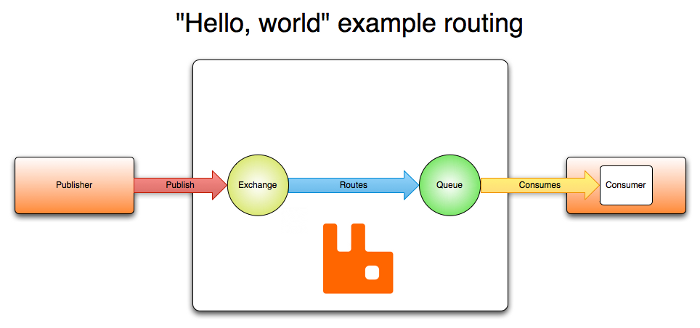
\includegraphics{assets/figures/rabbitmq.png}
    }
    \caption[\gls{AMQP} 0.9.1 Protocol Concepts]{\gls{AMQP} 0.9.1 Protocol Concepts by \cite{rabbitmqexpl}}
    \label{fig:implementation:decisions:rabbitmq}
 \end{figure}

As discussed in \citetitle{rabbitmqexpl}, there are four types of exchanges:

\begin{itemize}
    \item Direct Exchange: ideal for the unicast routing of messages;
    \item Fanout Exchange: ideal for the broadcast routing of messages;
    \item Topic Exchange: ideal for the multicast routing of messages, queues subscribe to specific routing keys;
    \item Header Exchange: ideal for more flexible unicast routing of messages, queues subscribe to specific message headers;
\end{itemize}

The exchange that better fits the defined requirements is the Topic Exchange.

When working with this protocol and type of exchange, some drawbacks were found:

When dealing with Topic Exchanges a Consumer can only subscribe to one specific routing key or all at once - via \textit{*}- this makes it complex to create routing keys with dynamic values. As an example, lets look at the \textit{Channel} routing key defined in Table~\ref{tab:design:domain:shared_model:routing} of Section~\ref{subsubsec:design:domain:shared_model:routing}. This key defines the single destination of a data unit. For a data unit to have various dynamic service destinations there would be a need to either:

\begin{itemize}
    \item Ensure that every single service subscribes to all relevant combinations of \textit{channel}s possible, deemed impractical;
    \item Duplicate data units, where each copy would be assigned a different channel, deemed inefficient;
\end{itemize}

To tackle this issue, another Message Broker, such as \citetitle{pulsar}, with its own protocol, can be used in the future. This Message Broker answers the drawback describe above by allowing Consumers to subscribe to multiple topics (equivalent to RabbitMQ' routing keys) on the basis of a regular expression (regex) [\citetitle{pulsarmulti}].

The other drawback found is that, according to the \citetitle{rabbitmqprotocol} the routing keys have a max size of 255 bytes. As described in Table~\ref{tab:design:domain:shared_model:routing} of Section~\ref{subsubsec:design:domain:shared_model:routing}, the system currently supports various keys and more keys are expected to be added in the future, meaning that this cap may one day be reached. This limitation was tackled by mapping each routing key to a single character when possible. As an example, the routing key \textit{Info Type Options} in Table~\ref{tab:design:domain:shared_model:routing} has three possible values: Encoded, Decoded and Processed, theses values are respectively represented in the system as \textit{e}, \textit{d} and \textit{p}.

\subsection{Usage of Protocol Buffers in Internal Communication}
\label{subsec:implementation:decisions:proto}

This section refers to how messages that flow in the system (via Message Broker) are serialized and deserialized. The common formats used to send structured data across systems are \gls{JSON} and \gls{XML}. This formats sacrifice size and de/serialization performance for human readability as stated by \cite{sumaray2012comparison}.

As mentioned before, \textbf{Sensae Console} aims to provide a good developer experience for external costumers that want to expand the solution according to their needs. Due to this, the final decision weighted heavily on formats that were self-documented, e.g. defined by a strict \textit{data schema}, such as \citetitle{proto} and \citetitle{thrift}.

These two technologies, \citetitle{proto} and \citetitle{thrift}, have similar goals and approaches to the problem they try to solve. They both rely on code generation based on a schema of the data structure. The tools related to this formats officially support various languages such as \textit{Java}, \textit{C++}, \textit{C\#}, \textit{Python}, \textit{Go} and others.

By leveraging these features, creating a basic \gls{SDK} in a new programming language is trivial since serialization, deserialization and data structure is already taken care by the code generation tool.

\citetitle{proto} are a ``language-neutral, platform-neutral, extensible mechanism for serializing structured data'' [\cite{proto}].

Thrift's ``primary goal is to enable efficient and reliable communication across programming languages by abstracting the portions of each language that tend to require the most customization into a common library that is implemented in each language'' [\cite{thrift}].

Ultimately \citetitle{proto} were chosen due to better documentation and community support.


\subsection{Database Usage throughout the Solution}
\label{subsec:implementation:decisions:database}

This section refers to how information is stored across the system.

A \gls{DBMS} is a general-purpose software system that facilitates the processes of defining, constructing, manipulating, and sharing data - \citetitle{elmasri2000fundamentals}. \gls{DBMS}s can be categorized according to several criteria, such as the data model, number of users or distribution. This section focus on the data model.

These are some of the data model types, according to \cite{elmasri2000fundamentals}:

\begin{itemize}
    \item The \textbf{relational data model} represents a database as a collection of tables,
    where each table can be stored as a separate file;
    \item The \textbf{document-based data model} is based on JSON (Java Script
    Object Notation) and stores the data as documents, which somewhat resemble
    complex objects;
    \item The \textbf{column-based data model} stores the columns of rows clustered on disk pages for fast access and allow multiple versions of the data;
    \item The \textbf{graph-based data model} stores objects as graph nodes and relationships among objects as directed graph edges;
    \item The \textbf{key-value data model} associates a unique key with each value (which can be a record or object) and provides very fast access to a value given its key.
\end{itemize}

The requirements gathered unveil the need to use three different database' data models throughout the system: (i) relational, (ii) document-based and (iii) column-based data models. The following sections answer why these data models were needed and what technologies were chosen for each of them. A final section unveils an optional solution that was considered but ultimately not pursued.

\subsubsection{Relational Database Usage}
\label{subsubsec:implementation:decisions:database:relational}

This data model has a wide variety of usage in the industry. Some of the technologies that follow this data model are: (i) \citetitle{mysql}, (ii) \citetitle{postgressql} and (iii) \citetitle{mariadb}.

It is intended for strictly structured data with well defined interrelations. This type of data can be found on most Bounded Contexts described in Section~\ref{subsec:design:domain:bounded_contexts} such as \nameref{subsubsec:design:domain:bounded_contexts:processor}, \nameref{subsubsec:design:domain:bounded_contexts:decoder}, \nameref{subsubsec:design:domain:bounded_contexts:device}, \nameref{subsubsec:design:domain:bounded_contexts:identity}, \nameref{subsubsec:design:domain:bounded_contexts:rule} and the Irrigation Zone/Device concepts of the \nameref{subsubsec:design:domain:bounded_contexts:irrigation} Context.

As such, this data model was adopted for the \textbf{Device Management Database}, \textbf{Data Decoder Database}, \textbf{Data Processor Database}, \textbf{Rule Management Database}, \textbf{Identity Management Database}, \textbf{Smart Irrigation Business Database} and \textbf{Notification Management Database} containers.

The author had previous contact with all the cited \gls{DBMS}, and the decision to use \citetitle{postgressql} was taken based on the fact that, contrary to the other options, \citetitle{postgressql} supports a vast number of Data Types such as \gls{JSON}, Arrays, \gls{UUID}, and Ranges. \citetitle{postgressql}'s data model is an extension of the relation data model, named object-relational data model - \cite{elmasri2000fundamentals}. This data model supports various concepts such as objects, classes and inheritance and therefore can lead to entity models more expressive and close to the business ideas.

\subsubsection{Document-based Database Usage}
\label{subsubsec:implementation:decisions:database:nosql}

This data model rose from the increasing need to store and analyze unstructured data as stated by \cite{miloslavskaya2016big}.  Citing \cite{elmasri2000fundamentals}, a ``major difference between document-based systems versus object and object-relational systems (relational database systems) is that there is no requirement to specify a schema''.

This type of requirements and data resembles the Data Store container described in Section~\ref{subsec:design:system_scopes:data_flow_scope} and Figure~\ref{fig:design:architecture:platform:container:process:diagram:flow}. This container, intended to mimic a Data Lake\footnote{Massively scalable storage repository that holds a vast amount of raw data in its native format («as is») until it is needed, by \cite{miloslavskaya2016big}}, stores any type of data for future use.

As such, this data model was adopted for the \textbf{Data Store Database} container.

The only technology considered, and therefore adopted, was \citetitle{mongodb} due to its vast community, excellent documentation and large number of libraries that ease the database management operations. \citetitle{mongodb} also supports replication and sharding. According to \cite{elmasri2000fundamentals}, these features are useful once a single node isn't capable of withstanding all data collected while providing fast access to it.

\subsubsection{Column-based Database Usage}
\label{subsubsec:implementation:decisions:database:time}

This data model is used in applications that require large amounts of data storage, and is commonly named \textit{data warehouses}. According to \cite{dehdouh2015using}, a data warehouse  is ``designed according to a dimensional modelling which has for objective to observe facts through measures, also called indicators, according to the dimensions that represent the analysis axes''. Citing \cite{han2011survey}, these databases ``can maintain high-performance of data analysis and business intelligence processing''.

These features fit the requirements related to storing and reading vast amounts of device measures. As such, it was adopter for the \textbf{Fleet Management Database} and \textbf{Smart Irrigation Data Database} containers.

The author had no previous contact with this type of data model. Some of the technologies related to this concept are: (i) \citetitle{hbase}, (ii) \citetitle{cassandradb}, (iii) \citetitle{influxdb}, (iv) \citetitle{questdb}.

According to \cite{george2011hbase} HBase is a ``distributed, persistent, strictly consistent storage system with near-optimal write and excellent read performance''. This database uses \gls{HDFS} as its file system, and so, it is built on top of Hadoop.
HBase does not support a structured query language like \gls{SQL}, ``even though it's comprised of a set of standard tables with rows and columns, much like a traditional database'' (\cite{ibm-hbase}).

CassandraDB is a distributed storage system for managing very large amounts of structured data spread out across many commodity servers, while providing highly available service with no single point of failure (\cite{lakshman2010cassandra}).
It was developed internally by Facebook and then later open-sourced to the Apache Foundation. It doesn't support \gls{SQL}.

According to \cite{naqvi2017time}, InfluxDB is an ``open-source schemaless \gls{TSDB} with optional closed-sourced components developed by InfluxData. It is written in Go programming language and it is optimized to handle time series data.'' It provides an SQL-like query language and also defines a new protocol for fast data ingestion (\cite{ilp}).

QuestDB is a relational column-oriented database designed for time series and event data and entitles it self as the ``fastest open source time series database'' (\cite{questdb}).
According to benchmarks (\cite{quest-bench}) preformed using the \gls{TSBS}, \cite{TSBS}, QuestDB ranks as the fastest option in the market.
It has out-of-the-box support for SQL Postgres wire protocol, (thus integrating with \gls{JDBC}), can be easily deployed using a single Docker Image, and also supports the \gls{ILP}.

The type of business this solution is tackling revolves around the capture and analysis of device readings, \gls{IoT}. So the notion of time has to be treated as a first class citizen. The measurements that constitute a time series are ordered on a timeline, which reveals information about underlying patterns.

As stated by \cite{naqvi2017time}, \gls{TSDB} ``can be used to efficiently store sensors and devices' data'' since, ``such technologies are generating large amount of data which is usually time-stamped''.

With this requirements in hand, a column-based data model isn't enough. The technology adopted should also natively support time series to ease data analysis. As such, the \citetitle{hbase} and \citetitle{cassandradb} options were discarded.

Between the two missing options, the author picked \citetitle{questdb} due to better support for \gls{SQL} though \gls{JDBC}. During the research of this two technologies no major downside was found for \citetitle{questdb} when compared to \citetitle{influxdb}.

\subsubsection{Graph-based Database Usage}
\label{subsubsec:implementation:decisions:database:identity}

Even tho this data model was ultimately not used, the author deemed relevant to analyze it.

As stated in the bounded context's section of~\nameref{subsubsec:design:domain:bounded_contexts:identity}, the domains follow a hierarchical structure that can resemble a graph. This context in particular would benefit from a  graph-based database, but this option was not pursued since the author had no previous contact with this family of technologies. Instead \citetitle{postgressql} was used.

\citetitle{postgressql} can represent logical hierarchical structures and concepts using the array data type as the \textit{path} from the root domain to the current domain.

Queries that revolve around graph concepts such as: select parent node, select child nodes, move nodes to a new parent and others, can be preformed efficiently using array operators such as \textbf{\&\&}, \textbf{||} and \textbf{@>}\footnote{taken from PostgresSQL Documentation: \citetitle{postgresarray} \& \citetitle{postgresarrayop}}.

\subsection{Rules Script Engine}
\label{subsec:implementation:decisions:drools}

This section refers to the bounded context of \textbf{Rule Management}. As mentioned before, the purpose of this context is to provide a high-level language that can analyze a stream of Data Units and output alerts base on them. The technology adopted was \citetitle{drools}.

\citetitle{drools} is an open-source rule engine widely used in the industry [\cite{droolsindustry}]. The features that stud out from other rule engines are:

\begin{itemize}
    \item Supports for sliding windows of time;
    \item It is also a \gls{CEP} System;
    \item Integrates with the \textit{iot-core} package since it is also written in \textit{Java};
    \item Can be used as a standalone application or an embedded component of another application;
    \item Has an expressive, yet complex, syntax to write rules;
    \item Can dynamically load rules at runtime.
\end{itemize}

The Section~\ref{subsec:implementation:description:rule} details how one can write rule scenarios.

\subsection{Data Decoders Script Engine}
\label{subsec:implementation:decisions:js}

This section refers to the bounded context of \textbf{Data Decoder}. As mentioned before, this context purpose is to translate inbound Data Units into a format and semantics that the system can understand. The technology adopted was \textit{Javascript}.

\textit{Javascript} is a high level language with an enormous community and is widely used in the industry. Another big reason behind this decision is that a lot of companies producing \gls{IoT} devices provide open-source decoders written in \textit{Javascript}, such as \href{https://github.com/Milesight-IoT/SensorDecoders}{Milesight} \footnote{\href {https://github.com/Milesight-IoT/SensorDecoders}{github.com/Milesight-IoT/SensorDecoders}}, \href{https://github.com/SensationalSystems}{SensationalSystems} \footnote{\href {https://github.com/SensationalSystems}{github.com/SensationalSystems}} and \href{https://github.com/helium/console-decoders}{Helium}, \footnote{\href {https://github.com/helium/console-decoders}{github.com/helium/console-decoders}}. This makes it easy and straightforward to integrate new decoders in \textbf{Sensae Console}.

The Section~\ref{subsec:implementation:description:decoder} details how one can write decoders.

\subsection{Containerization of services via Docker}
\label{subsec:implementation:decisions:docker}

This section describes how the final product is packaged into containers.

As stated in \citetitleyear{dockerinit}, Docker acts as an intermediary layer between the application to be deployed and the operating system where it will be deployed, ensuring that the developed software has the same behavior regardless of the system. The dependencies of the solution do not have to be present in the system, it is only necessary to install the Docker tool in the \gls{OS}.

This tool thus makes it possible to lower the coupling between the \gls{OS} and the software to be deployed.

With regards for this solution, each container defined in Section~\ref{sec:design:architecture} is mapped into a docker container.
A container is often compared to a virtual machine running on a hypervisor or \gls{OS}, but it has a much lower resource consumption, since only the application runs and not not all the processes inherent to an \gls{OS} as described by \cite{bernstein2014containers}.

The Figure~\ref{fig:implementation:decisions:docker:contvsvm} compares a \gls{VM} and Container-based deployments.

\begin{figure}[H]
    \centering
    \resizebox{0.7\columnwidth}{!}
    {
       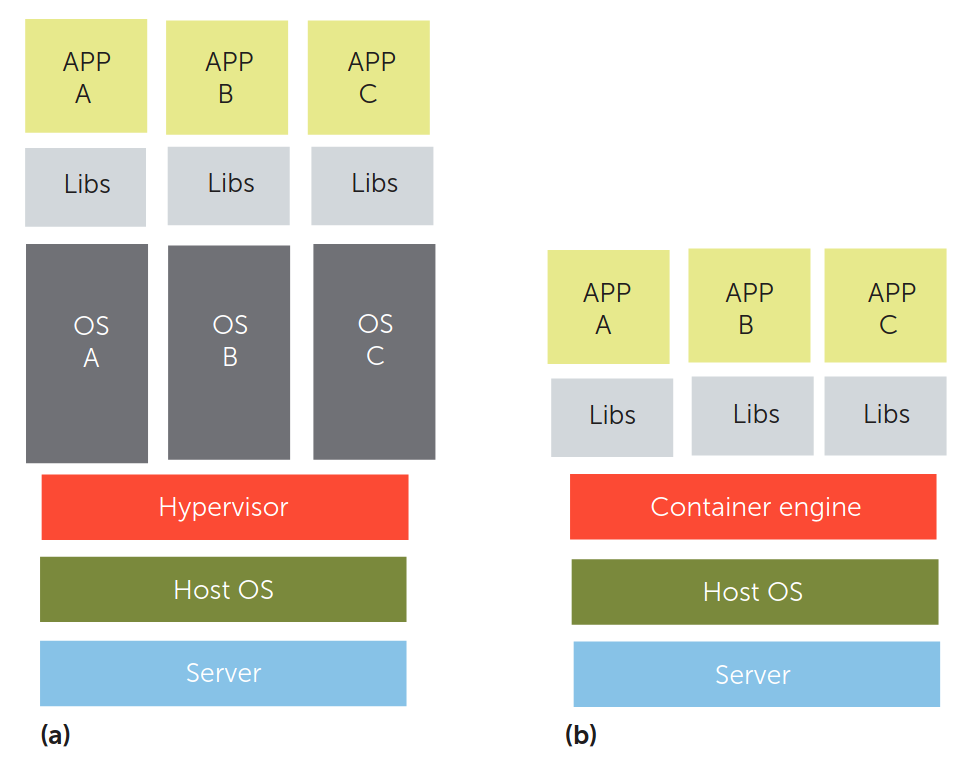
\includegraphics{assets/figures/vmvscontainer.png}
    }
    \caption[Comparison of VM and Container-based deployments]{Comparison of VM (a) and Container-based (b) deployments by \cite{bernstein2014containers}}
    \label{fig:implementation:decisions:docker:contvsvm}
\end{figure}

The system is thus represented as a collection of containers that communicate with each other and the outside through standard protocols such as HTTP or AMQP.

The production environment can thus be quickly replicated on another machine in case of a failure disaster or a overwhelming number of interaction with the server.

Details about service containerization can be found in Section~\ref{subsec:implementation:description:docker}.

\subsection{Orchestration of services via Docker Compose}
\label{subsec:implementation:decisions:compose}

This section describes how the final product is orchestrated using Docker Compose.

As stated in the article \citetitleyear{dockercompose}, ``Compose is a tool for defining and running multi-container Docker applications''.

Currently a single node is capable of handling the traffic generated by all the managed devices and costumers. Due to this, it was decided to use a docker compose in production inserted of tools like Kubernetes (that can ease the process of autoscaling individual containers).

The solution's orchestration is defined in a \textit{YAML} file and then started with a single command. To improve security, only the needed container ports are exposed. To ensure data integrity throughout service disruptions, persistence data is mapped to folder in the \gls{OS}. To ensure an easy management of the environment, configurations are kept in the \gls{OS} and fetched by each container once they start.

The details about the solution orchestration can be found in Section~\ref{subsec:implementation:description:compose}.

\subsection{Usage of Nginx as a web server and reverse proxy}
\label{subsec:implementation:decisions:nginx}

To serve the frontend pages and redirect requests made to backend containers, the following technologies were analyzed:

\begin{itemize}
    \item \citetitle{nginx};
    \item \citetitle{apachehttp};
    \item \citetitle{lighttpd}.
\end{itemize}

All of them support the necessary requirements, but some factors lead the author to pick Nginx over the others, the following table, Table~\ref{tab:implementation:decisions:nginx:compare}, describes this criteria.

\begin{table}[H]
    \caption{Technologies Comparison - Reverse Proxy Web Server}
    \label{tab:implementation:decisions:nginx:compare}
    \centering
    \begin{tabular}{@{}clll@{}}
    \toprule
    \textbf{Criteria/Technology} & \textbf{Nginx} & \textbf{Apache HTTP Server} & \textbf{Lighttpd} \\ \midrule
    Resource Consumption      & low  & high      & medium \\ \midrule
    Community Size            & high & very high & medium \\ \midrule
    Familiarity with the tool & high & low       & low    \\ \bottomrule
    \end{tabular}
\end{table}

The details about \citetitle{nginx} adoption and configuration can be found in Section~\ref{subsec:implementation:description:nginx}.

\subsection{Usage of Git as a version control system of the project}
\label{subsec:implementation:decisions:git}

\citetitle{git} is a \gls{VCS}. What differentiates it from other
systems such as \citetitle{mercurial} and \citetitle{bitkeeper} is its branching model. It is currently also the most widely used.

\citetitle{github} was the platform used to host the developed code. It offers private repositories with no additional costs. This platform also has other tools such as \textit{Github Issues} and \textit{Github Actions} that ease a developer's workflow.

A \gls{VCS} is indispensable in software development, this system allows developers to store the history of changes made to the code in an organized manner and simplifies the management of the software by the development team. This system was chosen over others because of the author was experienced with this software.

The development of the entire solution was made in two separated repositories, one for \textit{iot-core} and another for \textbf{Sensae Console}.

The \textit{iot-core} repository had a simple branching model consisting only of a master branch.

There was an extensive use of the branching feature in the repository of \textbf{Sensae Console}, following the model shown in Figure~\ref{fig:implementation:decisions:git:branch}. The author settled for the following: a master branch that matches the deployed version, a development branch where the various features are introduced until a new version is published on the master branch, several branches dedicated to fixing bugs (hotfix) and another several branches that introduce new features and improvements (feature \textit{x}).

\begin{figure}[H]
    \centering
    \resizebox{\columnwidth}{!}
    {
       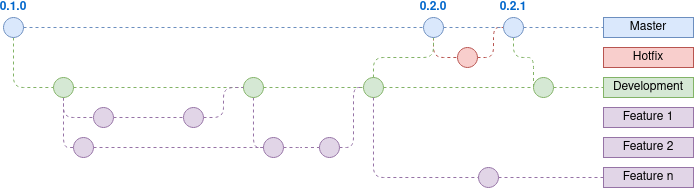
\includegraphics{assets/figures/branching-model.png}
    }
    \caption[Branching Model]{Branching Model}
    \label{fig:implementation:decisions:git:branch}
\end{figure}

This model was adopted since the project was in an initial phase of development, in the future, a branching model with multiple releases, as detailed in Figure~\ref{fig:implementation:decisions:git:branch2}, is preferred. With this model one can release only the altered containers and not the entire system.

\begin{figure}[H]
    \centering
    \resizebox{\columnwidth}{!}
    {
       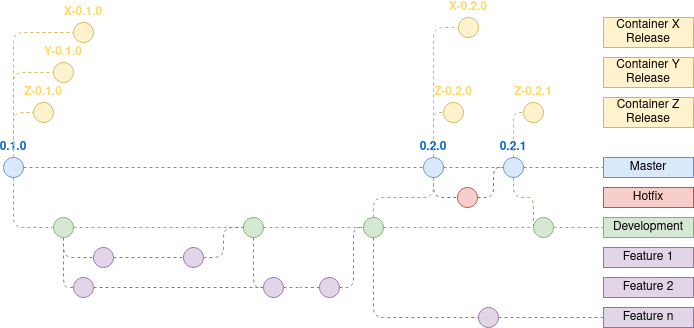
\includegraphics{assets/figures/branching-model-2.png}
    }
    \caption[Future Branching Model]{Future Branching Model}
    \label{fig:implementation:decisions:git:branch2}
\end{figure}

This is useful when using CI/CD pipelines to compile, package and deploy the various containers of the solution. If no changes have been made to \textit{X} Container there is no need to redo all the work previously done with it.

The reason behind the monorepo approach for \textbf{Sensae Console} is that it allows frontend libraries to be shared without publishing somewhere. It is also much easier to keep track of the code in a monorepo since the solution is developed by a single developer.

\subsection{Usage of Github Issues to track issues, bugs and new features}
\label{subsec:implementation:decisions:issues}

As described before, the code is hosted in \citetitle{github}. One of the services that this platform offers is \textit{Github Issues}. This tool helps to track and document the development process alongside with the code.

This tool can be separated into two main views. A view is concerned about what issues, features and bugs are active in the project, Figure~\ref{fig:implementation:decisions:issues:board}, and the other is concerned with the current state of each issue, feature and bug, Figure~\ref{fig:implementation:decisions:issues:project}.

\begin{figure}[H]
    \centering
    \resizebox{\columnwidth}{!}
    {
       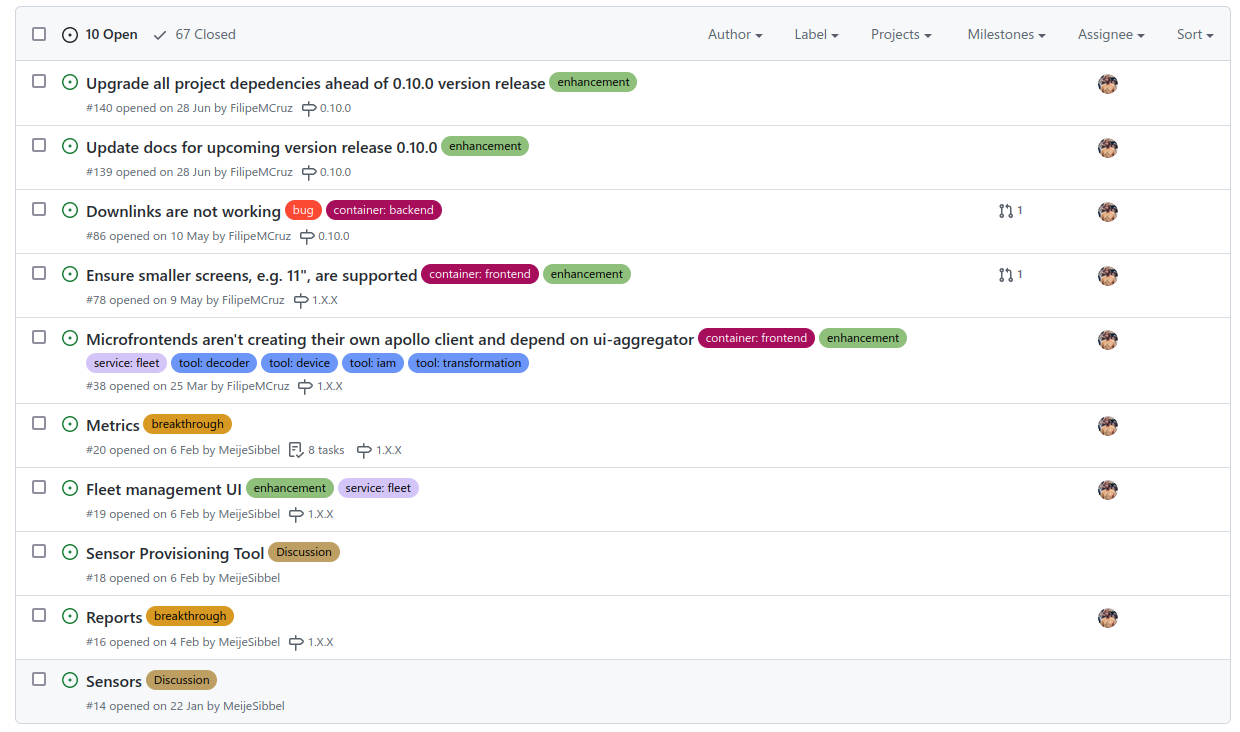
\includegraphics{assets/figures/github-2.png}
    }
    \caption[Github Issues]{Github Issues}
    \label{fig:implementation:decisions:issues:board}
\end{figure}

Each issue has a list of tags that represent its scope and a defined milestone. With this tool, the team members can also discuss issues in depth.

The issues presented in this page are then tracked in the \textit{project} page - Figure~\ref{fig:implementation:decisions:issues:project}. The author decided to divided the issues into 4 criteria:

\begin{itemize}
    \item \textbf{To Do}: Issues that have been discussed and are to be completed in the near future;
    \item \textbf{In Progress}: Issues that are currently under development and have an assigned feature branches;
    \item \textbf{Done}: Issues that have been completed and have been integrated in the \textit{master} branch;
    \item \textbf{Future}: Issues that have been purposed but have no clear deadline.
\end{itemize}

\begin{figure}[H]
    \centering
    \resizebox{\columnwidth}{!}
    {
       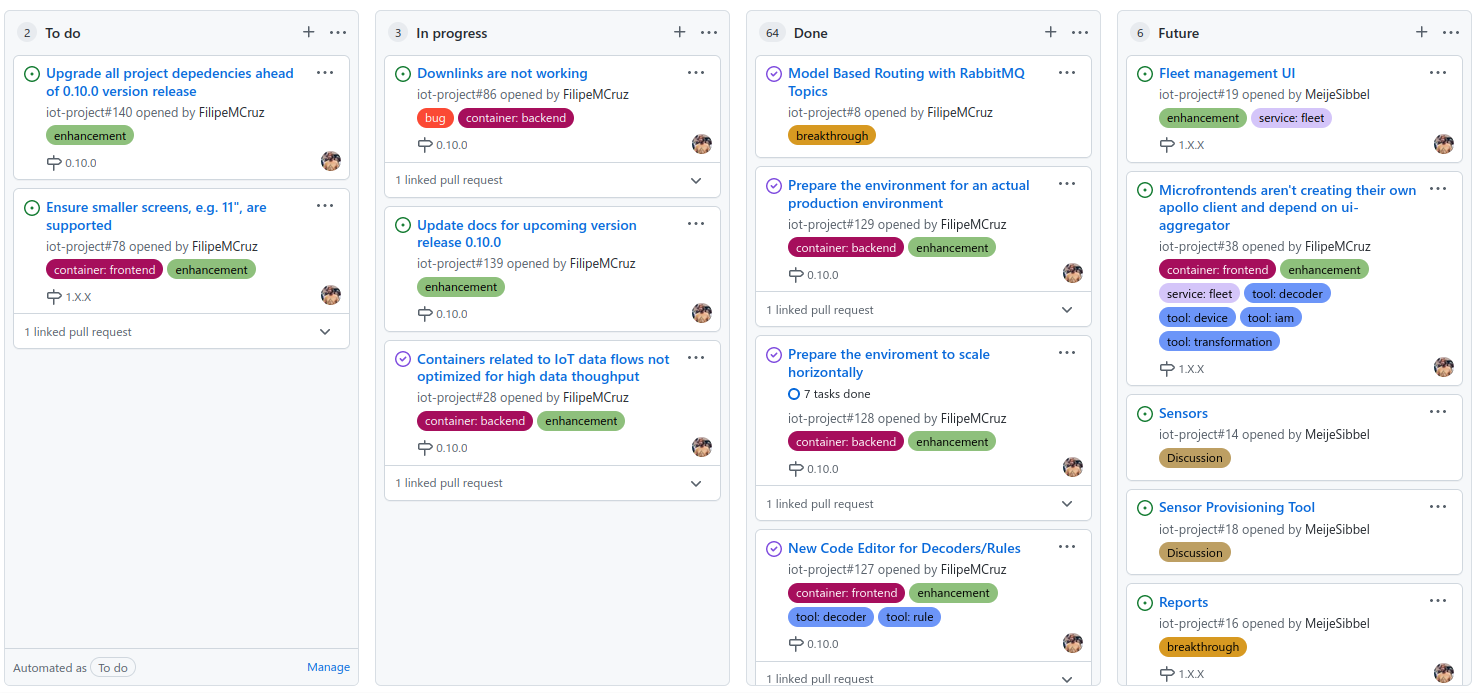
\includegraphics{assets/figures/github.png}
    }
    \caption[Github Issues Project Board]{Github Issues Project Board}
    \label{fig:implementation:decisions:issues:project}
\end{figure}

This view helps to define a simple project roadmap and track the overall state of issues, bugs and features in the project.

\subsection{Usage of Github Actions for CI/CD}
\label{subsec:implementation:decisions:actions}

Since the code is hosted in \textit{Github}, it was decided to leverage the CI/CD features of the platform. \textit{Github Actions} purpose is to automate software workflows via CI/CD.

According to \cite{cicd}, the term CI/CD represents a method to delivering applications to clients by introducing automation into the development states.
It is divided into three concepts:

\begin{itemize}
    \item \textbf{Continuous Integration}: new versions of the project are regularly submitted, tested and merged into the current project;
    \item \textbf{Continuous Delivery}: new versions of the project are automatically archived in a repository where they can then be deployed to a production environment;
    \item \textbf{Continuous Deployment}: new versions of the project are automatically deployed to a production environment.
\end{itemize}

The \textit{iot-core} package is archived in a repository so that it can then be integrated in the backend containers of \textbf{Sensae Console}, and possibly in other projects. To do so, the team uses \textit{Github Actions}. This tool's behavior is defined in a YAML file, presented in the Code Sample~\ref{code:implementation:decisions:actions:iotcore}.

\begin{lstlisting}[style=yaml, caption=Configuration File for \textit{iot-core} Continuous Delivery, label={code:implementation:decisions:actions:iotcore}]
name: IoT Core - Continuous Delivery to maven central
on:
  push:
    tags:
      - '**'
      - '*'
jobs:
  build:
    runs-on: ubuntu-latest
    steps:
      - uses: actions/checkout@v2
      - name: Set up Maven Central Repository
        uses: actions/setup-java@v1
        with:
          java-version: 17
          server-id: ossrh
          server-username: MAVEN_USERNAME
          server-password: MAVEN_PASSWORD
          gpg-private-key: ${{ secrets.MAVEN_GPG_PRIVATE_KEY }}
          gpg-passphrase: MAVEN_GPG_PASSPHRASE
      - name: Deploy with Maven
        run: mvn -B clean deploy -Pci-cd
        env:
          MAVEN_USERNAME: ${{ secrets.OSSRH_USERNAME }}
          MAVEN_PASSWORD: ${{ secrets.OSSRH_TOKEN }}
          MAVEN_GPG_PASSPHRASE: ${{ secrets.MAVEN_GPG_PASSPHRASE }}
\end{lstlisting}

As we can see in lines \textbf{2} to \textbf{6}, this action is triggered every time a new git tag is pushed to the repository.
This action then proceeds to download and setup java and maven - lines \textbf{12} to \textbf{20}. Finally it runs a maven command to deploy the new version to the artifact repository - lines \textbf{21} to \textbf{26}.

The \textbf{Sensae Console} has an action to deal with Continuous Integration - Code Sample~\ref{code:implementation:decisions:actions:cisensae}, where changes made to the software are tested.

\begin{lstlisting}[style=yaml, caption=Configuration File for \textbf{Sensae Console} Continuous Integration, label={code:implementation:decisions:actions:cisensae}]
name: Sensae Console - Continuous Integration - Test changes
on:
  push:
    branches:
      - master
      - dev
jobs:
  test:
    runs-on: ubuntu-latest
    steps:
      - uses: actions/checkout@v3
      - name: Set up JDK 17
        uses: actions/setup-java@v3
        with:
          java-version: "17"
          distribution: "adopt"
      - name: Set up Node 16
        uses: actions/setup-node@v3
        with:
          node-version: 16
      - name: Test Suite
        run: |
          ./project/scripts/run-tests.sh "${{ secrets.mapbox_token }}" "${{ secrets.microsoft_audience }}" "${{ secrets.google_audience }}" "${{ secrets.admin_email }}"

\end{lstlisting}

As we can see in lines \textbf{2} to \textbf{6}, this action is triggered every time a new commit is push to the \textit{dev} and \textit{master} branches.
This action then proceeds to download and setup java and maven - lines \textbf{10} to \textbf{16}, and then node and npm - lines \textbf{17} to \textbf{20}. Finally it runs a script that tests the solution - line \textbf{23}. The script requires the displayed secrets to run some tests, this tests will be discussed in the \nameref{sec:implementation:testing} Section.

The mentioned script has the following structure - Code Sample~\ref{code:implementation:decisions:actions:testscript}.

\begin{lstlisting}[language=bash, style=bash, caption=Sensae Console Test Suite Script, label={code:implementation:decisions:actions:testscript}]
#!/bin/bash
set -eo pipefail

ROOT_DIR=$(git rev-parse --show-toplevel)

cd "$ROOT_DIR"/project || exit

./scripts/generate-test-config.sh "$@"

docker-compose -f docker-compose.build.yml build

rm --f -- reports/backend-test-pass.log
rm --f -- reports/backend-test-fail.log

cd backend-services || exit

ls -I data-relayer | xargs -I % sh -c 'cd % && mvn test && \
    echo % >> ../../reports/backend-test-pass.log || \
    echo % >> ../../reports/backend-test-fail.log'

test ! -f ../reports/backend-test-fail.log

cd ../frontend-services || exit

npm install
npm run test-all

./../scripts/build-images.sh

docker-compose -f ../docker-compose.test.yml up -d --build

sleep 60

npm run e2e-all

docker-compose -f ../docker-compose.test.yml down
\end{lstlisting}

This script first intent is to defined a basic environment where tests can be run.
The flag \textit{set -eo pipefail} ensures that if any command fails the script will terminate and exit with an error.
It runs the following steps:

\begin{itemize}
    \item Generate configurations - line \textbf{8} - to run every test according to the secrets provided by the github action presented at Listing~\ref{code:implementation:decisions:actions:cisensae},
    \item Build the database containers - line \textbf{10}. The file \textit{docker-compose.build.yml} references all the solution's databases that need a custom build due to their predefined schema;
    \item Run the command \textit{mvn test} for all backend containers and store the results of each container's test in a file - lines \textbf{17} to \textbf{19};
    \item Checks if any container didn't pass the tests - line \textbf{15};
    \item Run tests related to the frontend at lines \textbf{23} to \textbf{26}. The script mentioned as \textit{test-all} is: \textit{nx run-many --all --target=test}. This script runs all unit tests of both frontend libraries and apps using \citetitle{nx}, as mentioned in \ref{subsubsec:implementation:decisions:frontend:nx} Section;
    \item Build and start an environment similar to the production one - lines \textbf{28} to \textbf{32};
    \item Preform end to end tests against the test environment - \textbf{34}. The script mentioned as \textit{e2e-all} is: \textit{nx run-many --all --target=e2e --parallel=1}. This script runs all end-to-end tests of the frontend apps using \citetitle{nx}, as mentioned in \ref{subsubsec:implementation:decisions:frontend:nx} Section;
    \item Shutdown the test environment.
\end{itemize}

\subsection{Usage of Maven Repository to host Open-Source Code}
\label{subsec:implementation:decisions:maven}

As stated in the previous section \textit{iot-core} is delivered to an artifact repository. Since the intent of this package is to be used by any one interested on integrating his/her tool with \textbf{Sensae Console}, the artifact repository has to be publicly available.

The Maven Central repository was the chosen one, since the \textit{maven} and \textit{gradle} tools use it, by default, to fetch dependencies.

According to the article \citetitle{centralreq} by \cite{centralreq}, to publish an artifact to maven central, a couple of additions have to be made in the \textit{pom.xml} of the project namely: (i) Supply Javadoc and Sources, (ii) Provide Files Checksums, (iii) Sign Files with GPG/PGP, (iv) Sufficient Metadata, (v) Correct Coordinates, (vi) Project Name, Description and URL, (vii) License Information, (vii) Developer Information, (viii) SCM Information.

In the Appendix~\ref{AppendixE} Appendix the full \textit{pom.xml} is presented.

\section{Technical Description}
\label{sec:implementation:description}

This section guides the reader through \textbf{Sensae Console} and \textbf{External Services} with a technical description of the various elements that are exposed to the final costumers and platform managers.

It describes the following topics:

\begin{itemize}
    \item \nameref{subsec:implementation:description:ui};
    \item \nameref{subsec:implementation:description:maps};
    \item \nameref{subsec:implementation:description:api};
    \item \nameref{subsec:implementation:description:ingestion};
    \item \nameref{subsec:implementation:description:rule};
    \item \nameref{subsec:implementation:description:decoder};
    \item \nameref{subsec:implementation:description:database};
    \item \nameref{subsec:implementation:description:docker};
    \item \nameref{subsec:implementation:description:compose};
    \item \nameref{subsec:implementation:description:nginx};
    \item \nameref{subsec:implementation:description:config};
    \item \nameref{subsec:implementation:description:services};
    \item \nameref{subsec:implementation:description:sensor};
\end{itemize}

\subsection{Sensae Console UI}
\label{subsec:implementation:description:ui}

In this subsection the \gls{UI} is presented.

The Figure~\ref{fig:implementation:description:ui:home} represents the main layout for any user. It is comprised of a toolbar with a section for \textbf{Service Pages}, another for \textbf{Configuration Pages} and a final one for authentication purposes.

\begin{figure}[H]
    \centering
    \resizebox{\columnwidth}{!}
    {
       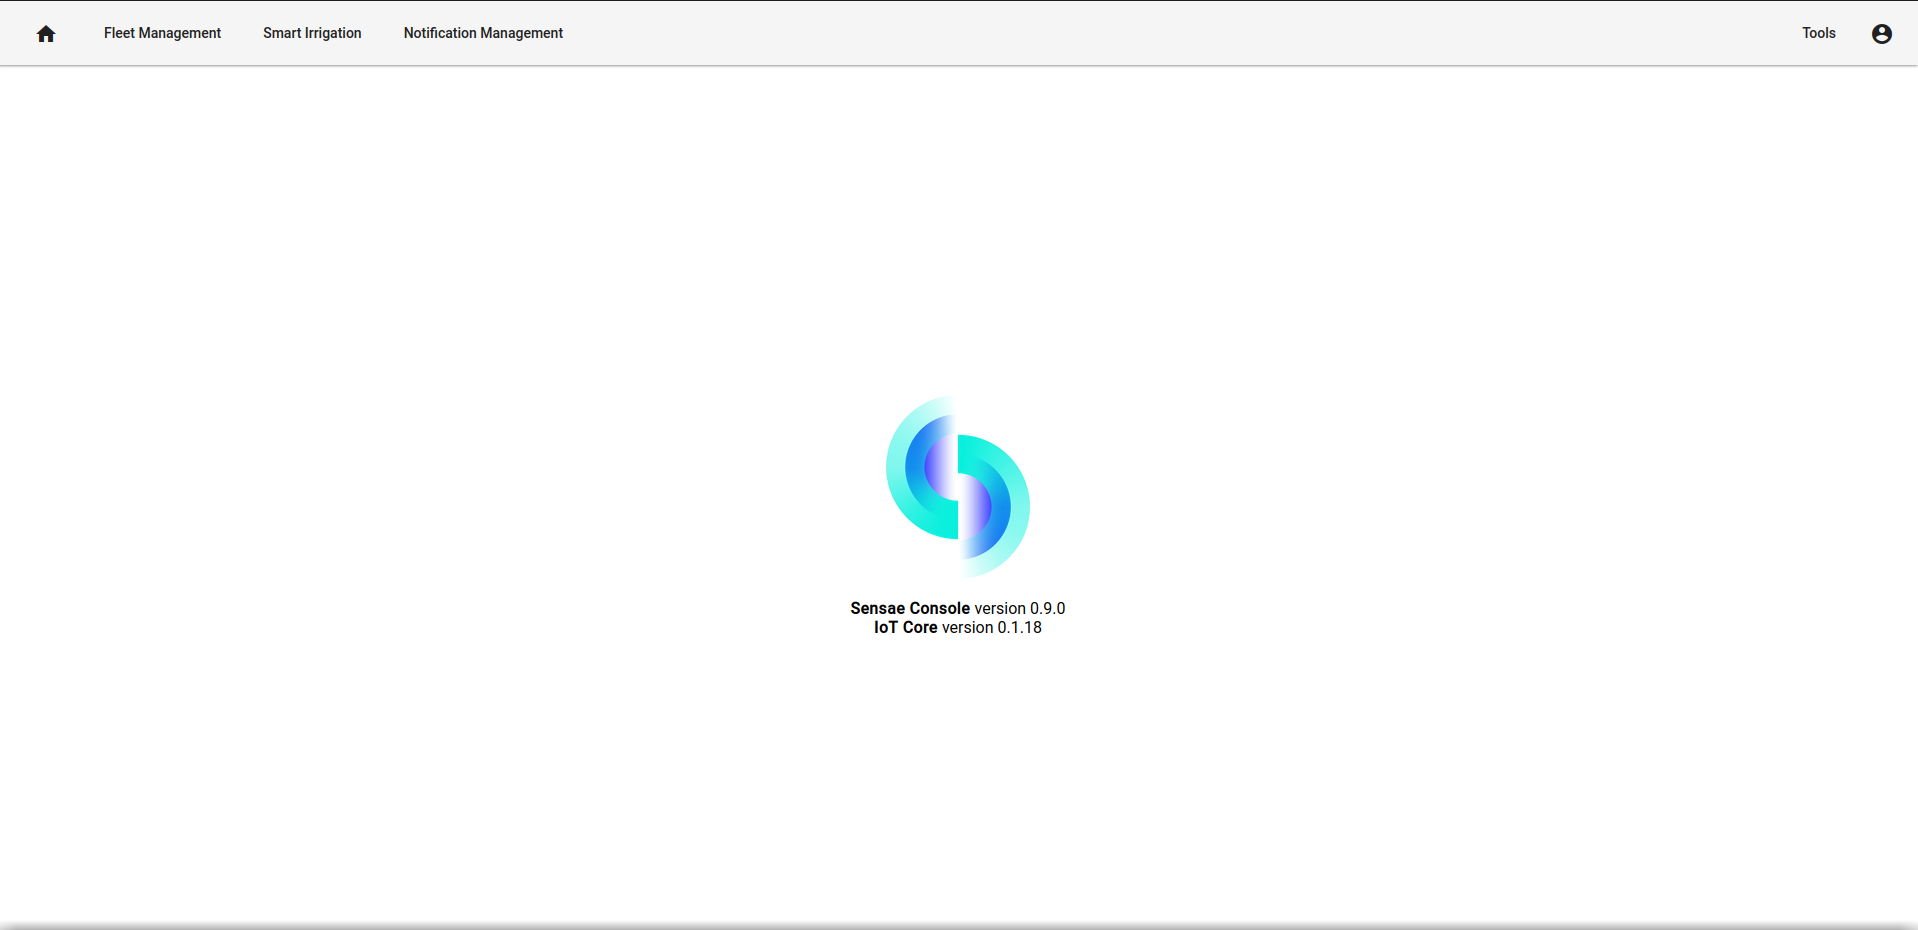
\includegraphics{assets/figures/ui/home.png}
    }
    \caption[Sensae Console Home Page]{Sensae Console Home Page}
    \label{fig:implementation:description:ui:home}
\end{figure}

From this page, if the user has sufficient permissions, he/she can access configuration pages, as an example the \textbf{Device Management Page} is displayed in Figure~\ref{fig:implementation:description:ui:device}.

\begin{figure}[H]
    \centering
    \resizebox{\columnwidth}{!}
    {
       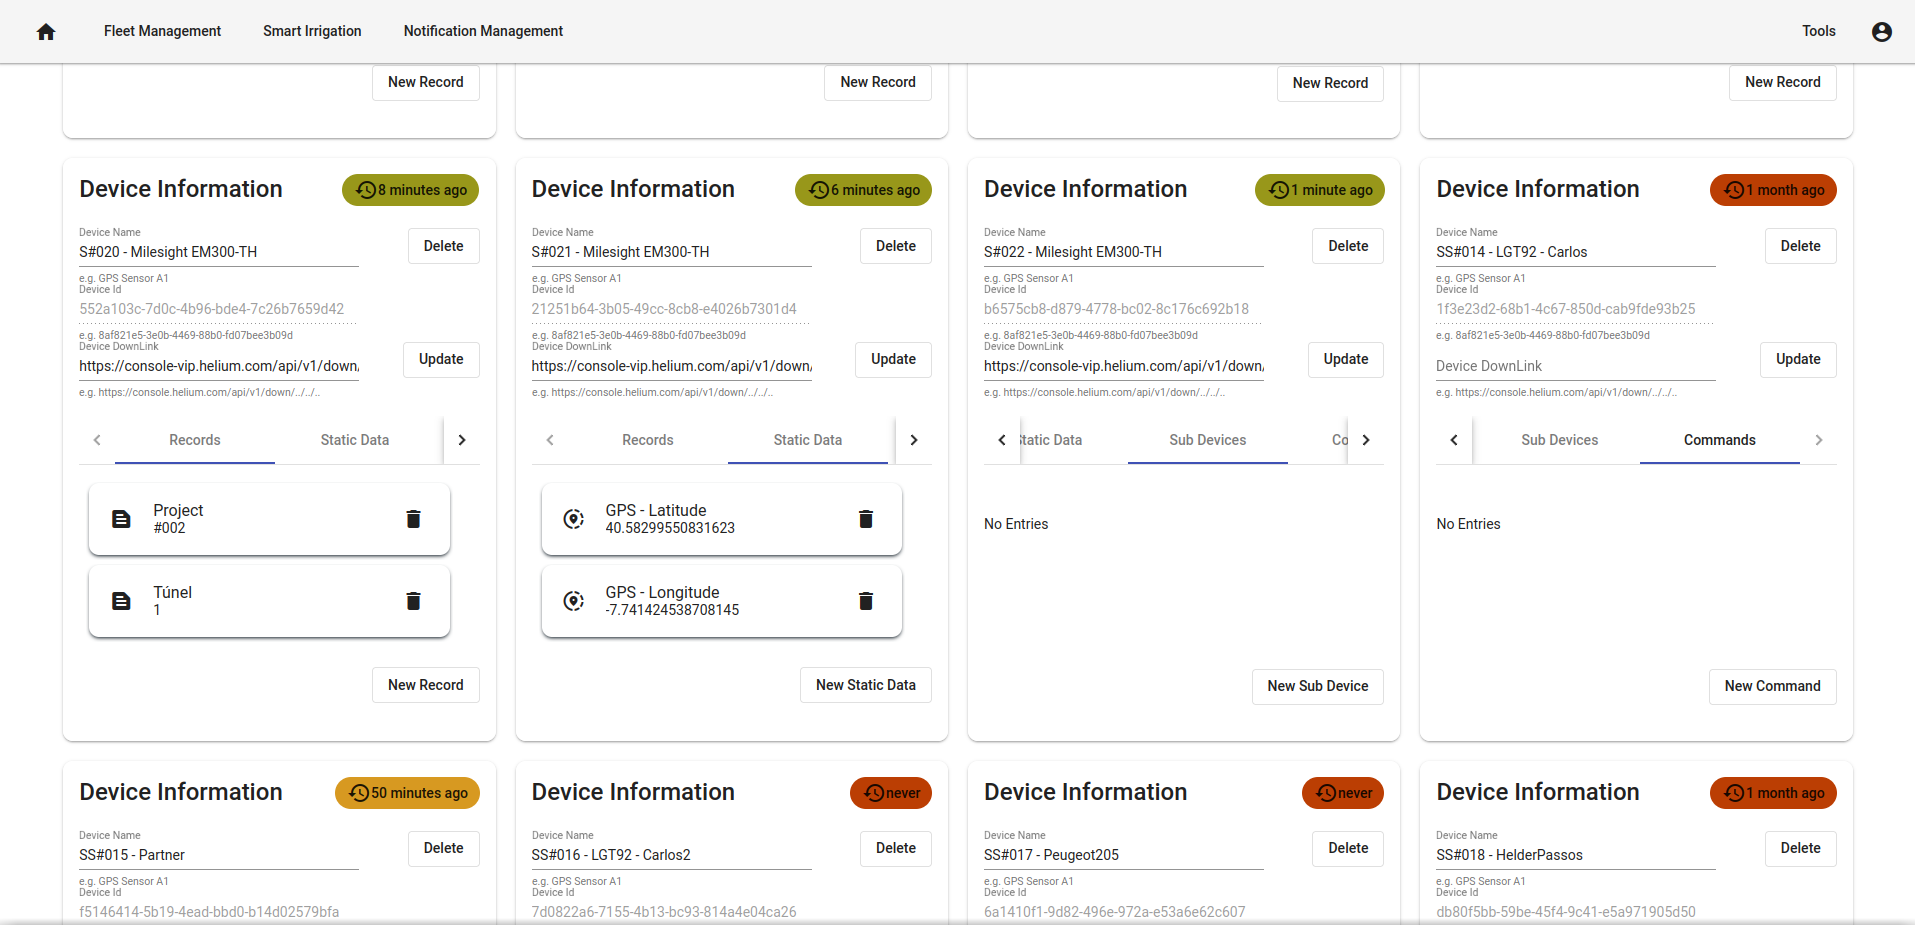
\includegraphics{assets/figures/ui/device-management.png}
    }
    \caption[Sensae Console Device Management Page]{Sensae Console Device Management Page}
    \label{fig:implementation:description:ui:device}
\end{figure}

In this page the user can see when was the last time the device interacted with the platform, create and delete devices and edit the details of each device according to the model presented in Section\nameref{subsubsec:design:domain:bounded_contexts:device} of the \textit{Bounded Contexts}.

From the home page, if the UI Aggregator was configured to fetch external services, one can access those services' pages too, as an example the \textbf{Smart Irrigation Page} is displayed in Figure~\ref{fig:implementation:description:ui:smartirrigation}.
This page presents a map where the user can see, search and create irrigation zones. Device measures are updated in real time via \textit{Websocket}s. The user can also see the irrigation zone details after clicking on it. From there it's possible to open/close valves an see the history of measures of each device.

\begin{figure}[H]
    \centering
    \resizebox{\columnwidth}{!}
    {
       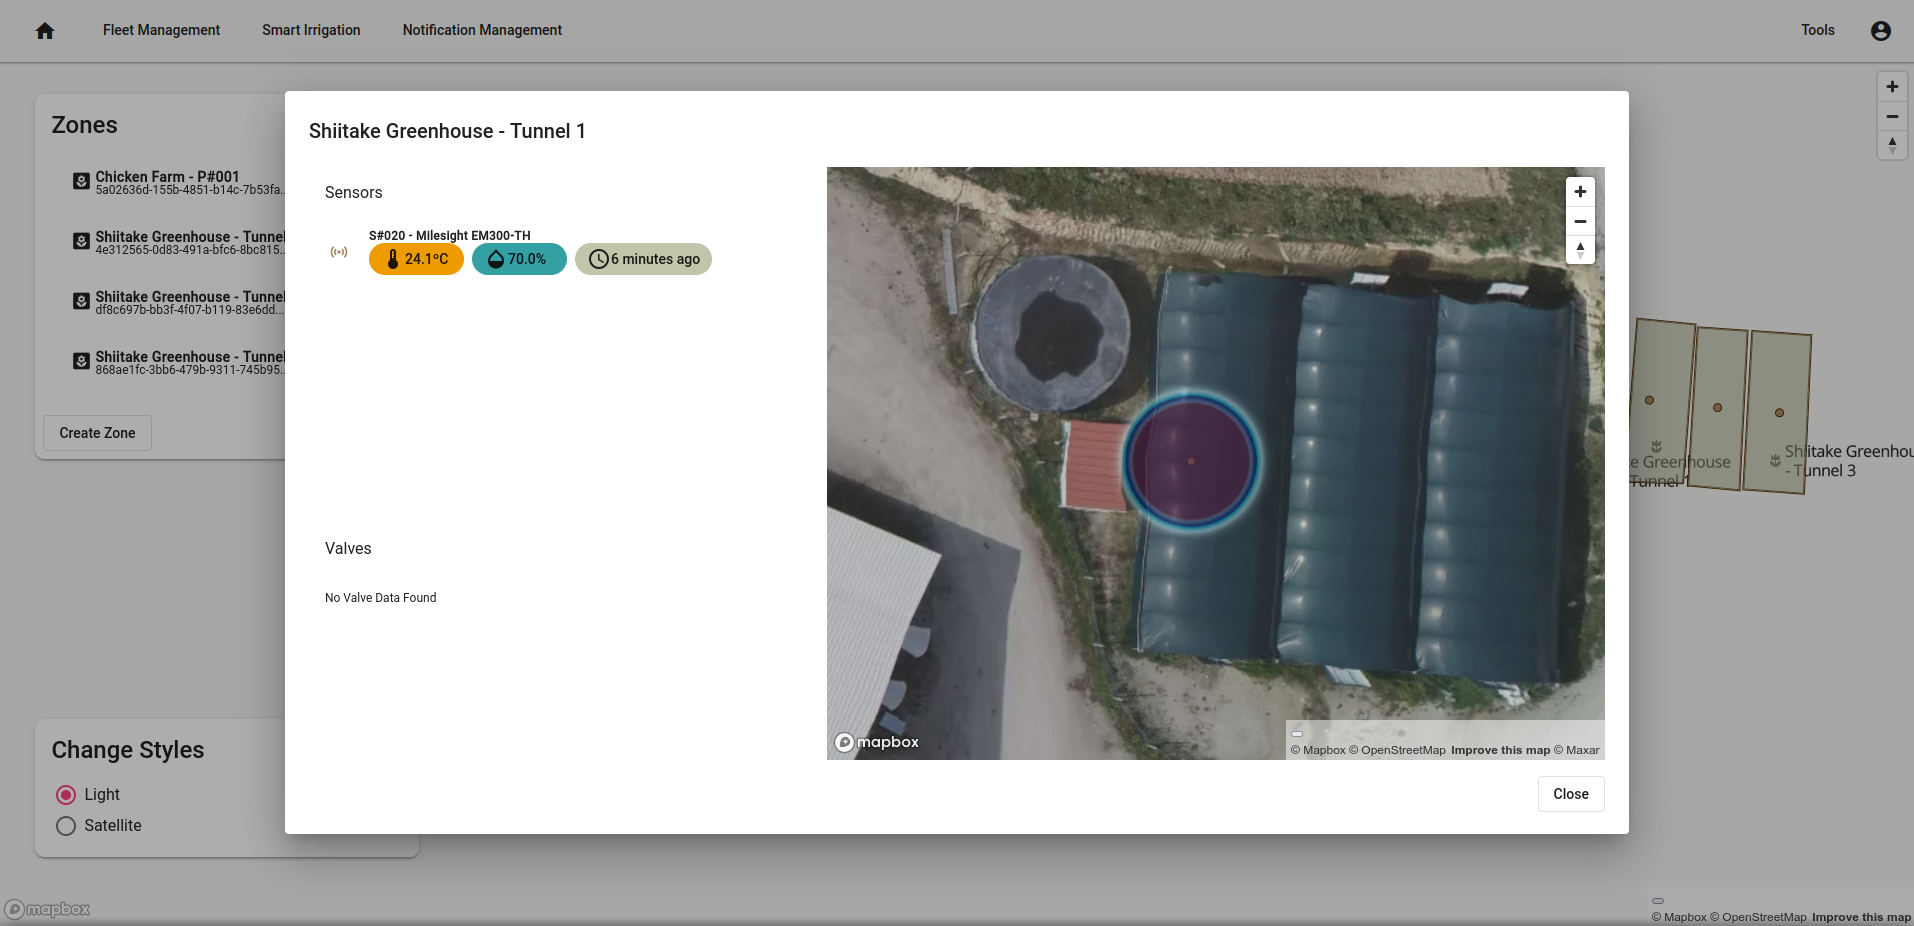
\includegraphics{assets/figures/ui/smart-irrigation.png}
    }
    \caption[Sensae Console Smart Irrigation Page]{Sensae Console Smart Irrigation Page}
    \label{fig:implementation:description:ui:smartirrigation}
\end{figure}

Other relevant pages are presented in the Appendix~\ref{AppendixD}, for Sensae Console, and Appendix~\ref{AppendixD2}, for the Solutions developed.

\subsection{Sensae Console Custom Maps}
\label{subsec:implementation:description:maps}

This section describes how custom maps where built to fit the solution needs. Some costumers facilities were not present in the satellite view of \citetitle{googlemaps} or \citetitle{mapbox}. A custom map, with the missing facilities, was built using satellite images taken with a drone. The images where processed with \citetitle{arcgis} and transformed in \textit{.tiff} files that could be incorporated in the basic satellite layer of \citetitle{mapbox}.

The following image, Figure~\ref{fig:implementation:description:maps:irrig} presents the new map with the costumer facilities in a greener tone than the rest of the map. This map was used to display three greenhouses and a chicken farm that belong to a costumer. This map is currently in use by the Smart Irrigation Service.

\begin{figure}[H]
    \centering
    \resizebox{\columnwidth}{!}
    {
       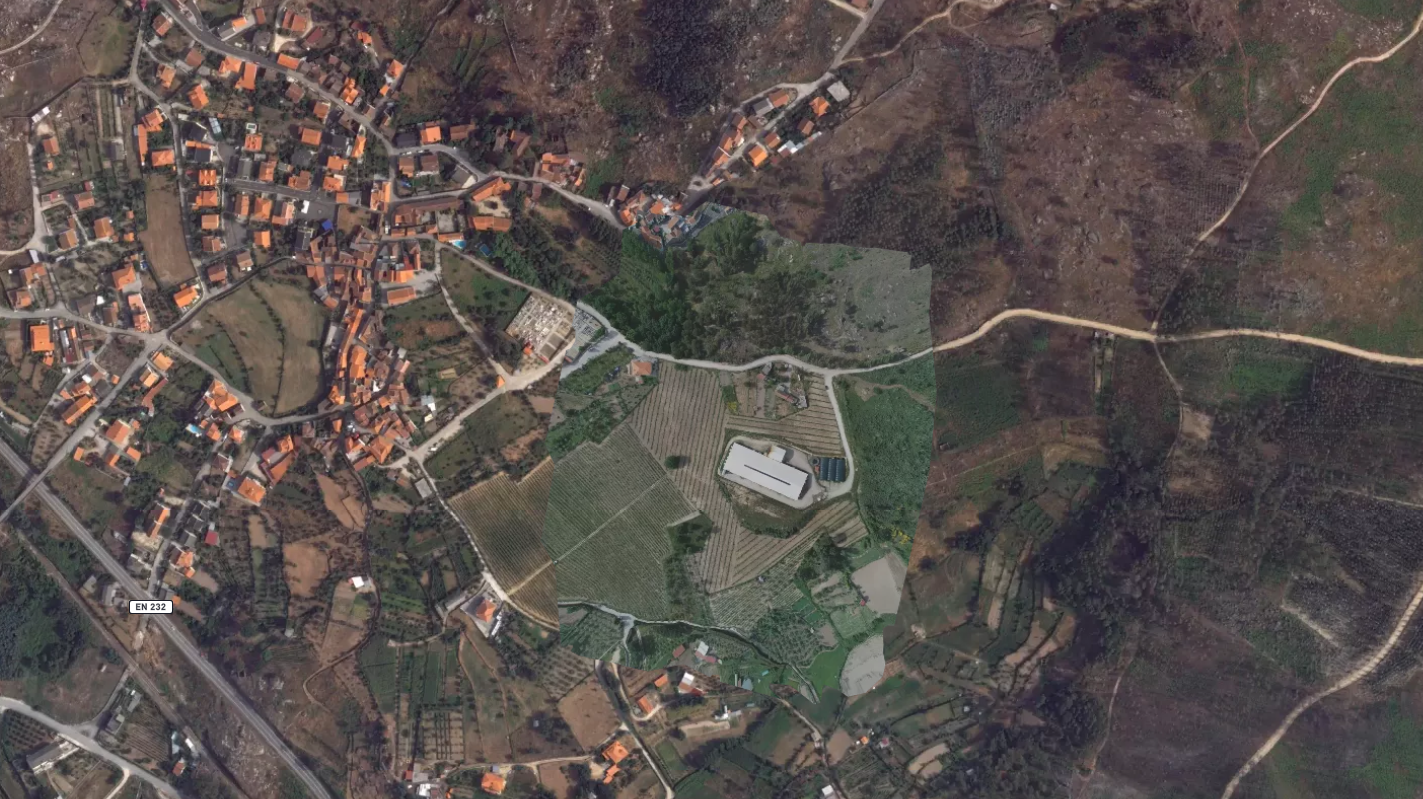
\includegraphics{assets/figures/maps/custom-map.png}
    }
    \caption[Custom Map - Smart Irrigation]{Custom Map - Smart Irrigation}
    \label{fig:implementation:description:maps:irrig}
\end{figure}

The road trajectory mismatch present in the map could be reduced by taking pictures from more angles. \citetitle{arcgis} would create better model with a wider pool of information.

\subsection{Sensae Console Backend API}
\label{subsec:implementation:description:api}

The \textbf{Sensae Console} \gls{API} is served as a \citetitle{graphql} \gls{API}, one for each service/configuration context. This \gls{API} is described with a schema.

As an example the Smart Irrigation API is presented in the Code Sample~\ref{code:implementation:description:api:irrigation}.

\begin{lstlisting}[caption=Smart Irrigation API Schema, label={code:implementation:description:api:irrigation}]
type Subscription {
    data(filters: LiveDataFilter, Authorization: String) : SensorData
}

type Query {
    history(filters: HistoryQueryFilters) : [SensorDataHistory]
    fetchIrrigationZones : [IrrigationZone]
    fetchLatestData(filters: LatestDataQueryFilters): [SensorData]
}

type Mutation {
    createIrrigationZone(instructions: CreateIrrigationZoneCommand) : IrrigationZone
    updateIrrigationZone(instructions: UpdateIrrigationZoneCommand) : IrrigationZone
    deleteIrrigationZone(instructions: DeleteIrrigationZoneCommand) : IrrigationZone
    switchValve(instructions: ValvesToSwitch): Boolean
}
\end{lstlisting}

From the observation of the code sample one can see that:

\begin{itemize}
    \item The \textit{data} function serves new \textit{SensorData} in real-time according to the filters provided in the \textit{filters} parameter;
    \item The textit{data} function uses \textit{Websocket} to operate as a full duplex communication channel. This spec, contrary to the HTTP spec does not account for HTTP Headers, as such the \gls{JWT} that provides the user authentication details has to be sent as a normal parameter and not as an Authorization HTTP Header.
    \item  There are three query type functions. One to fetch the history regarding Irrigation Zones or Devices over a time span. One to fetch the Irrigation Zones. And the last one to fetch the latest data of each device;
    \item There are four mutations, each corresponding to the use cases referenced in Section~\ref{subsubsec:requirements:functional:services:irrigation}.
\end{itemize}

\subsection{Sensae Console Data Ingestion Endpoint}
\label{subsec:implementation:description:ingestion}

The Data Ingestion Endpoint refers to how device data is sent to \textbf{Sensae Console}.

The endpoint corresponds to an HTTP POST verb with the following \gls{URL} schema:

\begin{verbatim}
    https://<ip>:<port>/sensor-data/{channel}/{infoType}/{deviceType}
\end{verbatim}

The endpoint collects the request body and then forwards it with the appropriate routing keys.

The routing keys are created according to the Table~\ref{tab:design:domain:shared_model:routing}. The \textit{infoType} can have two values: ENCODED or DECODED. Depending on this value the message is routed to \textit{Data Decoder Flow} or \textit{Data Processor Flow} as described in Figure~\ref{fig:design:architecture:platform:container:process:diagram:flow}.

The \textit{channel} parameter indicates the final service that it is destine to: \textit{fleet} for Fleet Management Service or \textit{irrigation} for Smart Irrigation Service. If another value is given the message is not routed to any service.

Finally, to ensure that the requests to this endpoint are trustworthy, a secret has to be sent in the Authorization HTTP Header. This secret is defined as a configuration of the \textbf{Sensae Console}, discussed in Section~\ref{subsec:implementation:description:config}.

\subsection{Sensae Console Rule Engine}
\label{subsec:implementation:description:rule}

The rule engine can be access from the \textbf{Rule Management Page} of the UI and, as stated in \nameref{subsubsec:design:domain:bounded_contexts:rule} Bounded Context, it provides a high-level language that can be used to detect anomalies in \textbf{Data Unit}s and turn them into \textbf{Alert}s.

Valid \textbf{Data Unit}s are captured by \textbf{Alert dispatcher Backend} and the inserted in the Rule Engine.

As stated in \nameref{subsec:implementation:decisions:drools}, the rule engine used was \citetitle{drools}. To write rules for \textbf{Sensae Console} one must follow several guidelines.

A \citetitle{drools} rule is composed by conditions, actions and facts.

Facts are inserted in the rule engine. If a fact or group of facts match a condition (\textit{when} section), an action is triggered (\textit{then} section).

The rule engine, is tailored to managers or developers and not for final clients since it can be hard to create meaningfully rules without side effects.

To clarify the guidelines the following Code Samples~\ref{code:implementation:description:rule:sample1}, ~\ref{code:implementation:description:rule:sample2} and \ref{code:implementation:description:rule:sample3} are presented.

The first Code Sample presents the beginning of the rule scenario, where imports and new Facts are created.

\begin{lstlisting}[style=drools, caption=Rule Scenario Example - Part 1, label={code:implementation:description:rule:sample1}]
package rules.project.two;

import pt.sharespot.iot.core.data.model.data.DataUnitReadingsDTO;
import pt.sharespot.iot.core.data.model.DataUnitDTO;
import pt.sharespot.iot.core.data.model.device.records. DeviceRecordEntryDTO;
import pt.sharespot.iot.core.data.model.properties.PropertyName;
import pt.sharespot.iot.core.alert.model.AlertBuilder;
import pt.sharespot.iot.core.alert.model.CorrelationDataBuilder;
import pt.sharespot.iot.core.alert.model.AlertLevel;
import java.util.List;
import java.util.UUID;

global pt.sharespot.iot.core.alert.model.AlertDispatcherService dispatcher;

dialect "mvel"

declare StoveSensor
    @role( event )
    deviceId : UUID
end

declare StoveSensorData
    @role( event )
    deviceId : UUID
    dataId : UUID
    temperature : Float
    humidity : Float
end
\end{lstlisting}

As we can see, from line \textbf{3} to \textbf{9}, classes from \textit{iot-core} are imported into the scenario.
At line \textbf{13} the interface that defines how an alert can be sent is imported for later use.
From line \textbf{17} to \textbf{28} two facts are declared, this can later be used as simple \textit{Java} POJOs. A fact defined with the \textit{event} role means that it occurred at a specific time (upon creation) and can be used for \gls{CEP}.

The following code sample presents a simple rule to store \textit{StoveSensorData} facts in the working memory of \citetitle{drools}.

\begin{lstlisting}[style=drools, caption=Rule Scenario Example - Part 2, label={code:implementation:description:rule:sample2}]
rule "Collect stove sensor data that belongs to Project #002"
    when
        $d : DataUnitDTO(
            getSensorData()
            .hasProperty(PropertyName.AIR_HUMIDITY_RELATIVE_PERCENTAGE),
            getSensorData()
            .hasProperty(PropertyName.TEMPERATURE)
        )
        exists DeviceRecordEntryDTO(
            label == "Project" && content == "#002"
        ) from $d.device.records
        not(StoveSensorData(dataId == $d.dataId))
    then
        StoveSensorData reading = new StoveSensorData();
        reading.setDeviceId($d.device.id);
        reading.setDataId($d.dataId);
        reading.setTemperature($d.getSensorData().temperature.celsius);
        reading.setHumidity($d.getSensorData().airHumidity .relativePercentage);
        insert(reading)
end
\end{lstlisting}

As we can see this rule is composed by two sections, the \textit{when} and \textit{then} sections. In the \textit{when} the following conditions are defined:

\begin{itemize}
    \item The captured DataUnitDTO has AIR HUMIDITY RELATIVE PERCENTAGE and TEMPERATURE measures - lines \textbf{3} to \textbf{8};
    \item The capture DataUnitDTO has a record with a "Project" label and "\#002" content - lines \textbf{9} to \textbf{11};
    \item The DataUnitDTO is not a duplicate fact in the working memory - line \textbf{12}.
\end{itemize}

Once this conditions are meet a \textit{StoveSensorData} is created with all the needed information and then inserted into the working memory - lines \textbf{14} to \textbf{19}.

The following code sample presents a simple rule to dispatch an \textbf{Alert} after some conditions are meet.

\begin{lstlisting}[style=drools, caption=Rule Scenario Example - Part 3, label={code:implementation:description:rule:sample3}]
rule "Dispatch Stove Alarm - Dry Soil Scenario - Project #002"
    when
        $s : StoveSensorData(temperature > 26, humidity < 50)
        not(StoveSensorData(this != $s,
                temperature < 26,
                humidity > 50,
                this after[0s,11m] $s)
        )
    then
        dispatcher.publish(AlertBuilder.create()
                            .setCategory("irrigation")
                            .setSubCategory("drySoilDetected")
                            .setDescription("Project #002 - Device "+ $s.deviceId +" detected low humidity/high temperature")
                            .setLevel(AlertLevel.ADVISORY)
                            .setContext(CorrelationDataBuilder.create()
                                .setDeviceIds($s.deviceId)
                                .setOther("Project #002")
                                .build())
                            .build());
end
\end{lstlisting}

As we can see this rule matches when the same device reports measures of air humidity higher than 50\% and temperature lower then 26 ºC for more than 11 minutes.

Once it matches an Alert is dispatched using the referenced dispatcher in Code Sample~\ref{code:implementation:description:rule:sample1}. The Alert can be created using the builder pattern.

An Alert closely resembles a Notification from the \nameref{subsubsec:design:domain:bounded_contexts:notification} Bounded Context. It also has a category (line \textbf{13}), a sub category (line \textbf{14}), a severity level (line \textbf{16}), a description (line \textbf{15}) and a notification context (lines \textbf{17} to \textbf{20}).

For an \textbf{Alert} to be sent at least the category and sub category parameters have to be set. By default the \textbf{INFORMATION} severity level is used.

In order for services to act upon a received \textbf{Alert}, it has to be associated with a \textit{DeviceId} (this association helps services like \textbf{Smart Irrigation} to know what Valve must be turned on or off), a \textit{DataId} or \textit{Other}.

An \textbf{Alert} is later transformed and store as a Notification, the \textit{DeviceId}s associated to it are used to determine what domains will have access to the Notification. If no \textit{DeviceId}s are associated only the root domain will have access to it.

\subsection{Sensae Console Data Decoders}
\label{subsec:implementation:description:decoder}

As mentioned in the \nameref{subsubsec:design:domain:bounded_contexts:decoder} Bounded Context Section, \textbf{Data decoder}'s purpose is to provide a flexible option to transform inbound data units into something that the system understands.

This happens when a \textbf{Data Unit} has a routing key with the ENCODED info type.

There are certain guidelines to follow in order to create a decoder:

\begin{itemize}
    \item Has to be written in vanilla \textit{javascript};
    \item Has to have an \textit{entry} function with the following signature \textit{function convert(dataUnit)};
    \item Can't import any node function, npm package or reference other scripts.
\end{itemize}

As an example, the Code Sample~\ref{code:implementation:description:decoder:em300th} presents the decoder for the device type EM500-TH\footnote{\href {https://www.milesight-iot.com/lorawan/sensor/em300-th}{Milesight EM300-TH Decoder}}.

\begin{lstlisting}[style=javascript, caption=EM300-TH Data Decoder Example, label={code:implementation:description:decoder:em300th}]
const decodePayload = (payload, port) =>
    ({"0": decoder(base64ToHex(payload), port)});

const base64ToHex = (() => {
    const values = [], output = [];

    return function base64ToHex(txt) {
        if (output.length <= 0) populateLookups();
        const result = [];
        let v1, v2, v3, v4;
        for (let i = 0, len = txt.length; i < len; i += 4) {
            v1 = values[txt.charCodeAt(i)];
            v2 = values[txt.charCodeAt(i + 1)];
            v3 = values[txt.charCodeAt(i + 2)];
            v4 = values[txt.charCodeAt(i + 3)];
            result.push(
                parseInt(output[(v1 << 2) | (v2 >> 4)], 16),
                parseInt(output[((v2 & 15) << 4) | (v3 >> 2)], 16),
                parseInt(output[((v3 & 3) << 6) | v4], 16)
            );
        }
        if (v4 === 64) result.splice(v3 === 64 ? -2 : -1);
        return result;
    };
    function populateLookups() {
        const keys =
            "ABCDEFGHIJKLMNOPQRSTUVWXYZabcdefghijkl mnopqrstuvwxyz0123456789+/=";
        for (let i = 0; i < 256; i++) {
            output.push(("0" + i.toString(16)).slice(-2));
            values.push(0);
        }
        for (let i = 0; i < 65; i++) values[keys.charCodeAt(i)] = i;
    }
})();

function decoder(bytes, port) {
    let decoded = {}, temperature = {}, airHumidity = {}, battery = {};
    for (let i = 0; i < bytes.length;) {
        let channel_id = bytes[i++];
        let channel_type = bytes[i++];
        if (channel_id === 0x01 && channel_type === 0x75) {
            decoded.battery = battery;
            battery.percentage = bytes[i];
            i += 1;
        } else if (channel_id === 0x03 && channel_type === 0x67) {
            decoded.temperature = temperature;
            temperature.celsius = readInt16LE(bytes.slice(i,i+2))/10;
            i += 2;
        } else if (channel_id === 0x04 && channel_type === 0x68) {
            decoded.airHumidity = airHumidity;
            airHumidity.relativePercentage = bytes[i] / 2;
            i += 1;
        } else {
            break;
        }
    }
    return decoded;
}
const readUInt16LE = bytes => (bytes[1] << 8) + bytes[0] & 0xffff;

function readInt16LE(bytes) {
    let ref = readUInt16LE(bytes);
    return ref > 0x7fff ? ref - 0x10000 : ref;
}
const convert = dataUnit => ({
    dataId: dataUnit.uuid,
    reportedAt: dataUnit.reported_at,
    device: {
        id: dataUnit.id,
        name: dataUnit.name,
        downlink: dataUnit.downlink_url,
    },
    measures: decodePayload(dataUnit.payload, dataUnit.port),
});
\end{lstlisting}

As we can see, this code sample decodes an EM300-TH \textbf{Data Unit}. The function \textit{convert} is the one mentioned in the guidelines, it assigns values such as \textit{id}, \textit{name}, \textit{reported\_at}, \textit{downlink\_url}, \textit{uuid} to its correct place and calls the function \textit{decodePayload} to gather the device measures. The \textit{decodePayload} stores every measure in the \textit{controller} key - value \textit{0}. The function \textit{base64ToHex} is the function that reads a Base 64 string and transforms it into a Hex Array - to reduce bandwidth the device normally encodes and sends data as a base 64 string. The function \textit{decoder}, \textit{readInt16LE} and \textit{readUInt16LE} were adapted from the TTN decoder\footnote{\href {https://www.milesight-iot.com/lorawan/sensor/em300-th}{Milesight EM300-TH Decoder}} of this device.

\subsection{Sensae Console Database Configuration}
\label{subsec:implementation:description:database}

The solution designed relies on various databases, and as discussed in Section~\ref{subsubsec:implementation:decisions:database:relational} some are relational databases. \citetitle{postgressql} and most databases of this data-model type require a database schema. For this solution the schema of each database is defined in a \textit{sql} file that is executed at the start of the database, only if no data is found.

Further database schema migrations are preformed using custom \gls{SQL} scripts when needed. In the future, once more instance of \textbf{Sensae Console} are deployed, the use of liquidbase or flyway is preferred.

The following Code Sample~\ref{code:implementation:description:database:file} exemplifies the content of this scripts.

\begin{lstlisting}[language=SQL, caption=Initialization Script Segment for Data Processor Database, label={code:implementation:description:database:file}]
create table if not exists public.transformation
(
    persistence_id bigint generated by default as identity
        primary key,
    device_type    varchar(255)
        constraint unique_type_constrain
            unique
);

create table if not exists public.property_transformation
(
    persistence_id                bigint generated by default as identity (maxvalue 2147483647)
        primary key,
    value                         integer           not null,
    old_path                      varchar(255),
    transformation_persistence_id bigint
        constraint ref_transformation_constrain
            references public.transformation,
    sub_sensor_id                 integer default 0 not null
);
\end{lstlisting}

This script defines two simple tables, \textit{transformation} and \textit{property\_transformation}, following the concepts defined in Section~\ref{subsubsec:design:domain:bounded_contexts:processor}.

Apart from the schema, the \textbf{Identity Management Database} also requires the following bootstrap data, as implied in \nameref{subsubsec:design:domain:bounded_contexts:identity} Bounded Context Section:

\begin{itemize}
    \item Root domain;
    \item Public domain;
    \item Unallocated Root domain;
    \item Anonymous Tenant account;
    \item Admin Tenant account;
\end{itemize}

This data is inserted using the following function, Code Sample~\ref{code:implementation:description:database:function}:

\begin{lstlisting}[language=SQL, caption=Bootstrap function for Identity Management Database, label={code:implementation:description:database:function}]
CREATE FUNCTION public.init_domains ()
RETURNS varchar(255) AS $root_oid$
    DECLARE
        root_oid varchar(255) := gen_random_uuid();
        public_oid varchar(255) := gen_random_uuid();
        unallocated_oid varchar(255) := gen_random_uuid();
    BEGIN
        INSERT INTO public.domain (name, oid, path)
        VALUES ('root', root_oid, ARRAY[root_oid]);
        INSERT INTO public.domain (name, oid, path)
        VALUES ('public', public_oid, ARRAY[root_oid, public_oid]);
        INSERT INTO public.domain (name, oid, path)
        VALUES ('unallocated', unallocated_oid, ARRAY[root_oid, unallocated_oid]);
        INSERT INTO public.tenant (name, oid, phone_number, email, domains)
        VALUES ('Anonymous', gen_random_uuid(), '', '', ARRAY[public_oid]);
        INSERT INTO public.tenant (name, oid, phone_number, email, domains)
        VALUES ('Admin', gen_random_uuid(), '', '$SENSAE_ADMIN_EMAIL', ARRAY[root_oid]);
        RETURN root_oid;
    END;
$root_oid$ LANGUAGE plpgsql;

select public.init_domains();

DROP FUNCTION public.init_domains;
\end{lstlisting}

This function starts by declaring three \gls{UUID} - lines \textbf{4} to \textbf{6} - that will later be used to populate the domain's \textit{path} and the tenant's \textit{domains} - lines \textbf{7} to \textbf{17}. In the end the function is executed and then removed to ensure that it isn't executed again.

In line \textbf{17}, the variable \textbf{\$SENSAE\_ADMIN\_EMAIL} is replace by a valid email before building the database container with the full script. This variable configuration is discussed in the Section~\ref{subsec:implementation:description:config}.

\subsection{Sensae Console Containerization}
\label{subsec:implementation:description:docker}

The section describes how \textbf{Sensae Console} is containerized with docker.
As explained in Section~\ref{subsec:implementation:decisions:docker}, the author choose to containerize the solution.

The following Code Samples describe how each container mentioned during the Design Chapter are packaged. To simplify, only three distinct samples will be presented.

The first sample, Listing~\ref{code:implementation:description:docker:frontend}, refers to UI Aggregator and is similar to all other frontend containers.

\begin{lstlisting}[caption=Dockerfile for UI Aggregator Frontend, label={code:implementation:description:docker:frontend}]
FROM node:18-alpine AS build
WORKDIR /workspace
COPY package.json ./
COPY . .
RUN npm install
RUN npm run nx build ui-aggregator --omit=dev

FROM nginx:1.23.1
COPY apps/ui-aggregator/nginx/nginx.conf /etc/nginx/conf.d/default.conf
COPY --from=build /workspace/dist/apps/ui-aggregator /usr/share/nginx/html
\end{lstlisting}

This Dockerfile contains two stages to reduce the size of the final image. The first stage, lines \textbf{1} to \textbf{6}, builds the project. The second one, containing only \citetitle{nginx} and the code that was previously built, is used to serve the UI Aggregator Frontend and route requests. The \citetitle{nginx} configuration file at line \textbf{9} is discussed in the \ref{subsec:implementation:description:nginx} Section.

The second sample, Listing~\ref{code:implementation:description:docker:spring}, refers to \textbf{Fleet Management Backend} and is similar to all backend containers in the Configuration Scope or External Services.

\begin{lstlisting}[caption=Dockerfile for Fleet Management Backend, label={code:implementation:description:docker:spring}]
FROM maven:3.8.5-openjdk-18 AS build
WORKDIR /app
# copy all pom.xml to pull only external dependencies
COPY application/pom.xml application/pom.xml
COPY domain/pom.xml domain/pom.xml
COPY infrastructure/boot/pom.xml infrastructure/boot/pom.xml
COPY infrastructure/endpoint/pom.xml infrastructure/endpoint/pom.xml
COPY infrastructure/persistence/pom.xml infrastructure/persistence/pom.xml
COPY infrastructure/persistence/questdb/pom.xml infrastructure/persistence/questdb/pom.xml
COPY infrastructure/endpoint/graphql/pom.xml infrastructure/endpoint/graphql/pom.xml
COPY infrastructure/endpoint/amqp/pom.xml infrastructure/endpoint/amqp/pom.xml
COPY infrastructure/pom.xml infrastructure/pom.xml
COPY pom.xml pom.xml
# build all external dependencies
RUN mvn -B -e -C org.apache.maven.plugins:maven-dependency-plugin:3.1.2:go-offline -DexcludeArtifactIds=fleet-management-backend,application,domain,infrastructure,endpoint,graphql,boot,amqp,questdb

COPY . .
RUN mvn clean package

FROM openjdk:17
WORKDIR /app
COPY --from=build /app/infrastructure/boot/target/fleet-management-backend.war /app
CMD ["java", "-jar", "fleet-management-backend.war"]
\end{lstlisting}

This sample also presents a multi-stage Dockerfile. The first stage, line \textbf{1} to \textbf{18} builds the project with Maven. All \textit{pom.xml} files and dependencies are added first to reduce build time during development, since these change less that the code written. The second stage is the one that runs the  service. It only contains the \gls{JDK} and the compiled application.

The third sample, Listing~\ref{code:implementation:description:docker:quarkus}, refers to \textbf{Device Commander} and is similar to all backend containers in the Data Flow Scope.

\begin{lstlisting}[caption=Dockerfile for Device Commander, label={code:implementation:description:docker:quarkus}]
FROM quay.io/quarkus/ubi-quarkus-native-image:22.1-java17 AS build
COPY --chown=quarkus:quarkus mvnw /code/mvnw
COPY --chown=quarkus:quarkus .mvn /code/.mvn
COPY --chown=quarkus:quarkus pom.xml /code/
USER quarkus
WORKDIR /code
RUN ./mvnw -B org.apache.maven.plugins:maven-dependency-plugin:3.1.2:go-offline
COPY src /code/src
RUN ./mvnw package -Pnative

FROM quay.io/quarkus/quarkus-micro-image:1.0
WORKDIR /work/
COPY --from=build /code/target/runner /work/application

# set up permissions for user `1001`
RUN chmod 775 /work /work/application \
    && chown -R 1001 /work \
    && chmod -R "g+rwX" /work \
    && chown -R 1001:root /work

EXPOSE 8080
USER 1001

CMD ["./application", "-Dquarkus.http.host=0.0.0.0"]
\end{lstlisting}

This sample, once again, is also a multi-stage Dockerfile. It was adapted from the one generated by \citetitle{quarkus} when setting up the application. In the first stage the application is built with a \citetitle{graalvm} native-image - lines \textbf{1} to \textbf{9}. This allows the image to run without \gls{JVM}. The second stage runs the service after setting user permissions, so that the process doesn't run as root, at lines \textbf{17} to \textbf{20}.

\subsection{Sensae Console Orchestration}
\label{subsec:implementation:description:compose}

As described in Section~\ref{par:design:architecture:platform:container:physical}, \citetitle{dockercompose} was the tool used to orchestrate the whole solution, the \textbf{Sensae Console} and External Services. This tool consumes a configuration file to know what containers, and their configurations, are needed. The complete configuration file for production is vast, a summarized version will be presented containing only the \textbf{Data Processor} Context' related containers.

\begin{lstlisting}[style=yaml, caption=Docker Compose Configuration File for Production, label={code:implementation:description:compose:file}]
services:
  data-processor-frontend:
    build:
      dockerfile: docker/data-processor-frontend/Dockerfile
      context: frontend-services
    image: data-processor-frontend
    volumes:
      - /etc/letsencrypt:/etc/letsencrypt/
      - /etc/nginx/ssl:/etc/nginx/ssl/
    networks:
      - sensae-network
    ports:
      - 443
    depends_on:
      - data-processor-master-backend
  data-processor-master-backend:
    build: backend-services/data-processor-master-backend
    image: data-processor-master-backend
    volumes:
      - ./secrets/keys:/etc/ssh/app
    environment:
      spring_profiles_active: prod
    env_file:
      - ./secrets/prod/data-processor-master-backend.env
    networks:
      - sensae-network
    ports:
      - 8080
  data-processor-database:
    build: databases/data-processor-database
    container_name: data-processor-database
    env_file:
      - ./secrets/prod/data-processor-database.env
    networks:
      - sensae-network
    ports:
      - 5482:5432
    volumes:
      - ./databases-data/prod/data-processor-database:/var/lib/postgresql/data/
  data-processor-flow:
    build: backend-services/data-processor-flow
    image: sensae/data-processor-flow
    env_file:
        - ./secrets/prod/data-processor-flow.env
    networks:
        - sensae-network
networks:
  sensae-network:
\end{lstlisting}

The following conclusions can be observed:

\begin{itemize}
    \item This context, similar to other contexts, is composed by four containers, a Frontend - \textit{data-processor-frontend}, a Configuration Backend - \textit{data-processor-master-backend}, a Database - \textit{data-processor-database}, and a Data Flow Backend - \textit{data-processor-flow};
    \item All services communicate in the same network - \textit{sensae-network};
    \item All services have instructions on how to build them;
    \item Various configuration files are loaded, e.g. in lines \textbf{19} to \textbf{20} and \textbf{28} to \textbf{31}, this files content will be discussed in the \nameref{subsec:implementation:description:config} Section;
    \item The Frontend has two volumes mapped, one loads the \textit{letsencrypt} configuration file for \citetitle{nginx} and the other loads the SSL certificate - lines \textbf{7} to \textbf{9}.
    \item The Configuration Backend needs to validate the authentication tokens received, for that, it has access to the public key that pairs the private key used to created then in \textbf{Identity Management Backend} - line \textbf{19} - \textbf{20};
    \item The database exposes a port to the host so that it can be managed remotely - lines \textbf{36} to \textbf{37};
    \item The database maps its data to a directory in the host, so that data is persisted between server restarts - lines \textbf{38} to \textbf{39};
    \item The Data Flow container doesn't need to expose any port since it only exchanges information with the message broker;
\end{itemize}

\subsection{Sensae Console Reverse Proxy Configuration}
\label{subsec:implementation:description:nginx}

This section reveals how \citetitle{nginx} is configured for all frontend containers in the solution. As an example, the Listing~\ref{code:implementation:description:nginx:irrig}, describes the \textbf{Smart Irrigation Frontend}.

\begin{lstlisting}[caption=Configuration File for Production Environment, label={code:implementation:description:nginx:irrig}]
server {

    server_name localhost;

    listen 443 ssl;

    ssl_certificate /etc/nginx/ssl/nginx.crt;
    ssl_certificate_key /etc/nginx/ssl/nginx.key;

    root        /usr/share/nginx/html;

    index       index.html index.htm;

    include /etc/letsencrypt/options-ssl-nginx.conf;

    location ~ .*remoteEntry.js$ {
        expires -1;
        add_header 'Cache-Control' 'no-store, no-cache, must-revalidate, proxy-revalidate, max-age=0';
    }

    location /smart-irrigation/graphql {
        proxy_pass http://smart-irrigation-backend:8080/graphql;
        proxy_set_header x-forwarded-prefix /smart-irrigation/graphql;
        proxy_set_header Host $host;
        proxy_set_header x-forwarded-host $host;
        proxy_redirect off;
        proxy_set_header x-forwarded-port 443;
        proxy_set_header x-forwarded-proto https;
    }

    location /smart-irrigation/subscriptions {
        proxy_pass http://smart-irrigation-backend:8080/subscriptions;
        proxy_set_header x-forwarded-prefix /smart-irrigation/subscriptions;
        proxy_http_version 1.1;
        proxy_set_header Upgrade $http_upgrade;
        proxy_set_header Connection "Upgrade";
        proxy_set_header Host $host;
        proxy_read_timeout 6000;
        proxy_send_timeout 6000;
        proxy_redirect off;
        proxy_set_header x-forwarded-port 443;
        proxy_set_header x-forwarded-proto https;
    }

    location / {
        try_files $uri $uri/ /index.html;
    }

    if ($scheme != "https") {
        return 301 https://$host$request_uri;
    } # managed by Certbot
}
\end{lstlisting}

The following conclusions can be inferred:

\begin{itemize}
    \item It only exposes the HTTPS port - line \textbf{4} and lines \textbf{49} to \textbf{51};
    \item It loads the SSL certificates mapped in the \citetitle{dockercompose} file - lines \textbf{7} and \textbf{8};
    \item It uses the \textit{letsencrypt} configuration - line \textbf{14};
    \item The \textit{remoteEntry} file, responsible for providing the entry point to the service in a Micro Frontend environment, is never cached in the client browser since it points to the current compiled version of the service. If this file is cached, the updated version of a micro frontend, can only be accessed by the client browser once the local cache is cleaned up - lines \textbf{16} to \textbf{19};
    \item The \citetitle{graphql} endpoint is defined as a reverse proxy endpoint. Requests made to \textit{/smart-irrigation/graphql} are routed to \textit{http://smart-irrigation-backend:8080/graphql}. It doesn't use a secure connection, HTTPS, since this communication already happens inside the docker network where man in the middle attacks are disregarded - lines \textbf{21} to \textbf{29};
    \item The \citetitle{graphql} subscription endpoint is also defined, this type of connection, \textit{Websocket}, requires the use of HTTP version 1.1 and the two Headers presented at lines \textbf{34} to \textbf{36};
    \item All other requests are handled in lines \textbf{45} to \textbf{47}.
\end{itemize}

\subsection{Sensae Console Configuration Files}
\label{subsec:implementation:description:config}

This section describes how a \textbf{Sensae Console} and External Services are configured. One of the problems that arise from a microservice architecture is how to maintain all configurations for each container developed and configured. Following the \citetitle{confcentral}, all configurations are defined via configuration files that support three environments: \textit{dev}, \textit{test} and \textit{prod}.

This configurations are defined, for each environment, in a single file. This file, Listing~\ref{code:implementation:description:config:file}, has the following structure:

\begin{lstlisting}[language=bash, style=bash, caption=Configuration File for Production Environment, label={code:implementation:description:config:file}]
export SENSAE_MAPBOX_ACCESS_TOKEN=
export SENSAE_MAPBOX_SIMPLE_STYLE=
export SENSAE_MAPBOX_SATELLITE_STYLE=
export SENSAE_BROKER_USERNAME=
export SENSAE_BROKER_PASSWORD=
export SENSAE_COMMON_DATABASE_PASSWORD=
export SENSAE_DATA_STORE_USER_PASSWORD=
export SENSAE_DATA_STORE_ROOT_PASSWORD=
export SENSAE_AUTH_PATH_PUB_KEY=
export SENSAE_AUTH_PATH_PRIV_KEY=
export SENSAE_AUTH_ISSUER=
export SENSAE_AUTH_AUDIENCE=
export SENSAE_DATA_AUTH_KEY=
export SENSAE_AUTH_EXTERNAL_MICROSOFT_AUDIENCE=
export SENSAE_AUTH_EXTERNAL_GOOGLE_AUDIENCE=
export SENSAE_SMS_TWILIO_ACCOUNT_SID=
export SENSAE_SMS_TWILIO_AUTH_TOKEN=
export SENSAE_SMS_SENDER_NUMBER=
export SENSAE_SMS_ACTIVATE=
export SENSAE_EMAIL_SENDER_ACCOUNT=
export SENSAE_EMAIL_SUBJECT=
export SENSAE_EMAIL_SENDER_PASSWORD=
export SENSAE_EMAIL_SMTP_HOST=
export SENSAE_EMAIL_SMTP_PORT=
export SENSAE_EMAIL_ACTIVATE=
export SENSAE_PROD_PUBLIC_DOMAIN=
export SENSAE_ADMIN_EMAIL=
\end{lstlisting}

This file variables are then passed on to each container's environment configuration file with the help of a script. The Code Sample~\ref{code:implementation:description:config:script} sheds a light on how the script propagates the configurations.

\begin{lstlisting}[language=bash, style=bash, caption=Configuration Propagation Script, label={code:implementation:description:config:script}]
#!/usr/bin/sh

ROOT_DIR=$(git rev-parse --show-toplevel)

cd "$ROOT_DIR"/project || exit

. ./secrets/prod.conf

SECRET_BACK=secrets/templates/prod/backend-services
SECRET_FRONT=secrets/templates/prod/frontend-services
SECRET_DB=secrets/templates/prod/databases

BACK_PREFIX=secrets/prod
FRONT_PREFIX=frontend-services/apps
FRONT_SUFFIX=src/environments/environment.prod.ts

envsubst < $SECRET_BACK/alert-dispatcher-backend.env > \
     $BACK_PREFIX/alert-dispatcher-backend.env
# and all other backend services
envsubst < $SECRET_BACK/data-validator.env >
     $BACK_PREFIX/data-validator.env

envsubst < $SECRET_FRONT/device-management-frontend.ts > \
 $FRONT_PREFIX/device-management-frontend/$FRONT_SUFFIX
# and all other frontend services
envsubst < $SECRET_FRONT/ui-aggregator.ts > \
 $FRONT_PREFIX/ui-aggregator/$FRONT_SUFFIX

envsubst < secrets/templates/prod/message-broker/message-broker.env > \
 $BACK_PREFIX/message-broker.env

envsubst < $SECRET_DB/data-decoder-database.env > \
 $BACK_PREFIX/data-decoder-database.env
# and all other databases
envsubst < $SECRET_DB/rule-management-database.env > \
 $BACK_PREFIX/rule-management-database.env
\end{lstlisting}

In the future, as more isolated deployments are made, a tool such as \citetitle{vault} should be integrated in the solution.

\subsection{Solutions - External Services}
\label{subsec:implementation:description:services}

This section discusses how external services interact with the Sensae \gls{API}, this was briefly mentioned in Section~\ref{subsubsec:design:domain:shared_model:routing}.

In order to provide an easy to understand integration with the platform, the routing keys concept was introduced. The idea, from the point of view of someone developing a service, is to start by defining what type of information that service should capture.

The two types of information a service usually needs are: (i) \textbf{Data Unit}s and (ii) \textbf{Alert}s. Each of this information are defined by their routing keys as described in Table~\ref{tab:design:domain:shared_model:routing}.

A service can also publish \textbf{Command}s.

The following sub sections will detail each service information needs.

\subsubsection{Fleet Management Service}
\label{subsubsec:implementation:description:services:fleet}

The focus of this service was to simply collect the location of the costumers' fleet since the company was given no permission to access the vehicles' \gls{OBD} System. Access to the \gls{OBD} System would provide a deeper knowledge regarding the vehicles' conditions.

Therefore, this service captures information of a single type (and doesn't publish any Command):

\textbf{Data Topic}: \textit{'processed'}, \textit{'correct'}, with \textit{'defined ownership'} and \textit{'device information'} data unit with \textit{'gps'} readings in the channel \textit{'fleet'}.

At a high-level view, this service only requires \gls{GPS} data sent to the \textit{'fleet'} channel.

\subsubsection{Notification Management Service}
\label{subsubsec:implementation:description:services:notification}

The focus of this service was to simply showcase and dispatch the alerts sent by \textbf{Sensae Console}. A simple rule scenario for Indoor Fire Detention was then created based on tests performed on a costumer's facilities (Appendix \ref{AppendixH}). The rule scenario was based on the following metrics: CO2 \gls{PPM}, Air humidity and Air Temperature.

This service captures information of a single type (and doesn't publish any Command):

\textbf{Alert Topic}: alerts with \textit{'defined ownership'}.

At a high-level view, this service requires all alerts that already have a \textit{'defined ownership'}.

It is divided in two backend containers (as described in Figure~\ref{fig:design:architecture:solutions:containers:logical:noti}) that subscribe to the same information but handle it differently.

\subsubsection{Smart Irrigation Service}
\label{subsubsec:implementation:description:services:irrigation}

The focus of this service was on the two most common types of agriculture mentioned in literature, outdoor and greenhouse, according to \cite{garcia2020iot}.

The Greenhouse agriculture type collects two measures: (i) Air Temperature and (ii) Air Humidity, the Outdoor agriculture also collects two measures: (i) Luminosity and (ii) Soil Moisture. Both rely on a irrigation system that can be activated and deactivated remotely, like a simple switch, to regulate the monitured environment.

The measures to capture were chosen according to costumers' sugestions and \cite{garcia2020iot} that states that the Soil moisture, Air Temperature, Air Humidity and Luminosity parameters are the most common monitured parameters in papers that propose an irrigaiton system. 

This service captures information of the given types:

\begin{itemize}
    \item \textbf{Data Topic}: \textit{'processed'}, \textit{'correct'}, with \textit{'defined ownership'} and \textit{'device information'} data unit with \textit{'gps'} and \textit{'trigger'} readings in the channel \textit{'irrigation'} (for valves);
    \item \textbf{Data Topic}: \textit{'processed'}, \textit{'correct'}, with \textit{'defined ownership'} and \textit{'device information'} data unit with \textit{'gps'}, \textit{'temperature'} and \textit{'air humidity'} readings in the channel \textit{'irrigation'} (for green house sensors);
    \item \textbf{Data Topic}: \textit{'processed'}, \textit{'correct'}, with \textit{'defined ownership'} and \textit{'device information'} data unit with \textit{'gps'}, \textit{'illuminance'} and \textit{'soil moisture'} readings in the channel \textit{'irrigation'} (for park sensors);
    \item \textbf{Alert Topic}: alerts with the category \textit{'smartIrrigation'} and sub category \textit{'drySoil'} (to open all valves in a garden);
    \item \textbf{Alert Topic}: alerts with \textit{'defined ownership'}, the category \textit{'smartIrrigation'} and sub category \textit{'moistSoil'} (to close all valves in a garden);
    \item \textbf{Alert Topic}: alerts with \textit{'defined ownership'}, the category \textit{'smartIrrigation'} and sub category \textit{'valveOpenForLengthyPeriod'} (to close that specific valve).
\end{itemize}

It then publishes Commands to close or open valves. The service can only issue a command if the Data Unit sent by the valve refers two commands, one to open and another to close the valve. This commands, usually defined in the \textbf{Device Management Page}, and mentioned in the \nameref{subsubsec:design:domain:bounded_contexts:device} Bounded Context, need to have the \textit{CommandId} value as \textit{'openValve'} or \textit{'closeValve'}.

At a high-level view, this service requires data from \textit{Park} sensors, \textit{Green Houses} and \textit{Valves} that flow in the \textit{'irrigation'} channel. It captures Alerts to decide when to open or close Valves by sending specific Commands.

\subsection{Sensae Console Device Integration}
\label{subsec:implementation:description:sensor}

This section describes how devices can be connected to \textbf{Sensae Console}. As stated in Section~\ref{sec:requirements:non_functional}, the service that must be used to communicate with devices is \citetitle{helium}. This solution works with other platforms, such as Azure IoT Hub, since it provides an agnostic data ingestion endpoint as stated in Section~\ref{subsec:implementation:description:ingestion}.

Virtually any device can be integrated, via \citetitle{helium}, with \textbf{Sensae Console}. To do so, one needs to register new devices in \citetitle{helium}, for example via \gls{OTAA}. Then create a Custom HTTP Integration, following the Section~\ref{subsec:implementation:description:ingestion} instructions.

The Figure~\ref{fig:implementation:description:sensor:integration} presents an example of the custom integration for the EM300-TH Device.

\begin{figure}[H]
    \centering
    \resizebox{\columnwidth}{!}
    {
       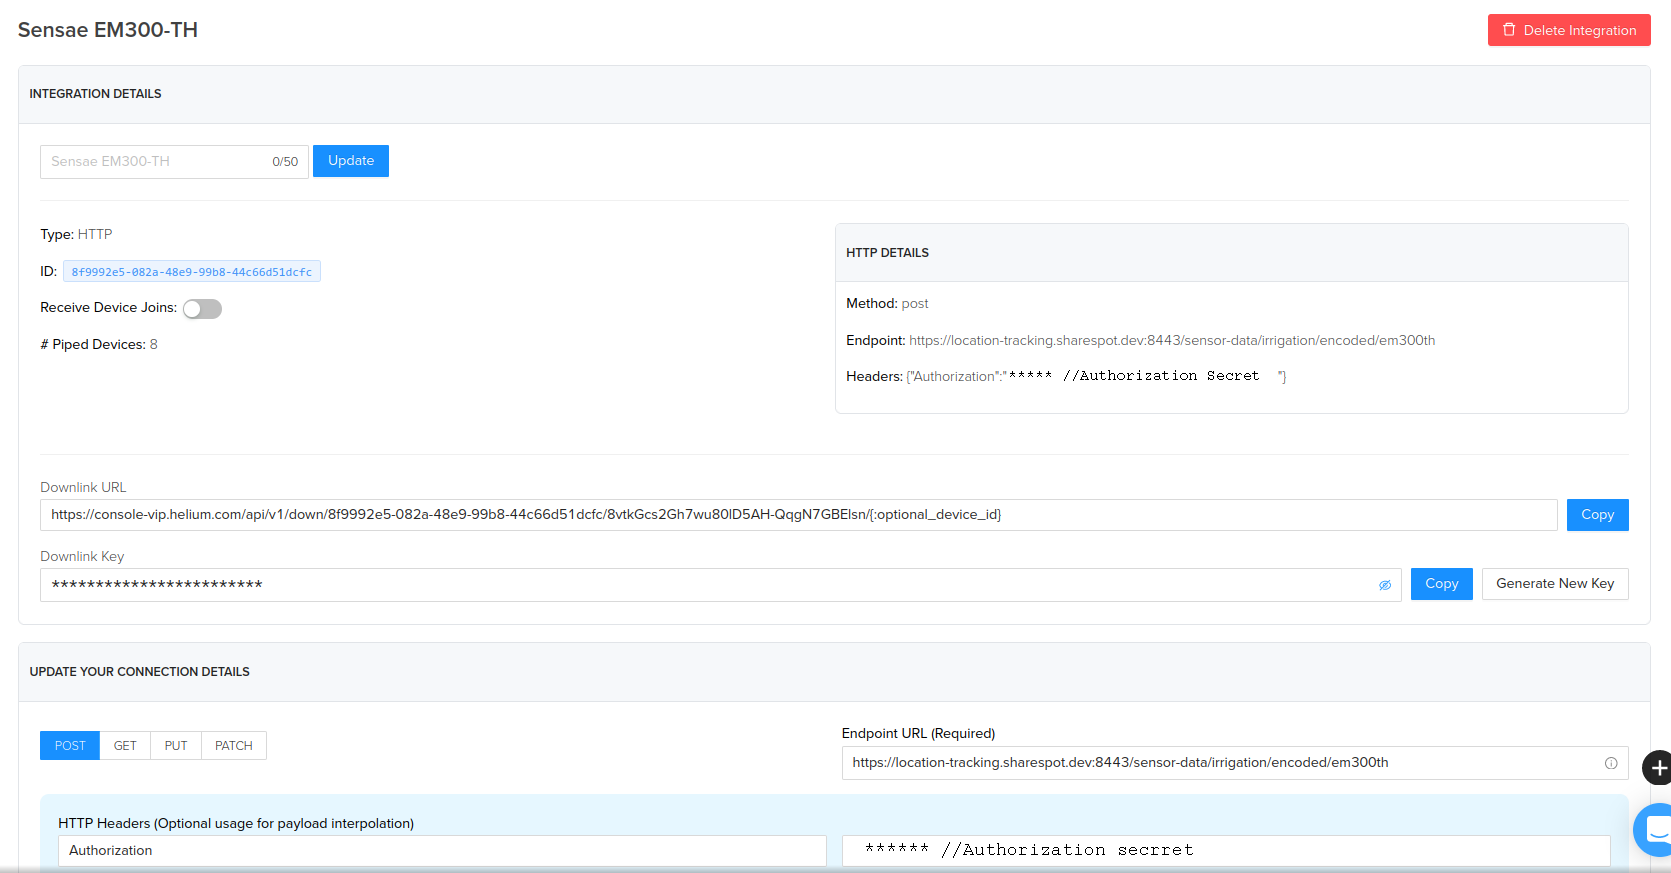
\includegraphics{assets/figures/sensor/integration.png}
    }
    \caption[Helium Custom Integration Page]{Helium Custom Integration Page}
    \label{fig:implementation:description:sensor:integration}
\end{figure}

Finally, in the \citetitle{helium} flows page, connect the registered device to the custom integration.

This method will require the user to register the endpoint with the \textit{encoded} type and write a \textbf{Data Decoder} in \textbf{Sensae Console} to translate the payload sent by the device though \citetitle{helium}.

If the user intends to use the \textbf{Data Processor}, he/she needs to:

\begin{itemize}
    \item Register the endpoint with the \textit{decoded} type;
    \item Define a \textbf{Data Processor} in \textbf{Sensae Console} to map the payload sent by \citetitle{helium};
    \item Write the decoder in \citetitle{helium} - in the \textit{Function} page;
    \item Link the device to the \textit{Function} in \citetitle{helium};
    \item Link the \textit{Function} to the custom integration;
\end{itemize}

\section{Testing}
\label{sec:implementation:testing}

According to \cite{booktest}: ``Software testing is the activity of running a series of dynamic executions of software programs after the software source code has been developed.''
Tests have a fundamental role in the development of software, they validate the the work done, prevent production bugs, regressions and improve code quality, according to \cite{linuxtest} and \cite{imbtest}.

According to \cite{typetest} there are seven categories of tests:

\begin{itemize}
    \item \textbf{Unit Testing}: Capture the need to verify and validate the individual behavior of small pieces of the solution.
    \item \textbf{Integration Testing}: Capture the need to verify that different modules/components of the system work collectively as expected;
    \item \textbf{Functional Testing}: Capture the need to verify that business requirements are meet by the system;
    \item \textbf{End-to-End Testing}: Capture the need to verify that user interaction against common workflows works as expected in the system;
    \item \textbf{Acceptance Testing}: Capture the need to ensure that functional and non-functional requirements are accomplished;
    \item \textbf{Performance Testing}: Capture the need to verify how the environment behaves under heavy load. Their objective is to evaluate the stability, availability and reliability of the system;
    \item \textbf{Smoke Testing}: Capture the need to verify the overall state of the system before running heavier and extensive tests.
\end{itemize}

These categories complement each other to ensure the correct behavior of the system. Nevertheless, the Smoke and Acceptance Testing categories were not pursuit.

The smoke tests were replaced by common unit tests. The acceptance tests weren't required since, at the time of writing, the project had no clear and concise functional requirements that the platform could be tested against.

Architectural tests were added to the test suite to ensure that the Design discussed in the \nameref{par:design:architecture:platform:components:logical} Section would always be respected.

The performance tests will be discussed in depth in the \nameref{chap:evaluation} Chapter.

In the following sections examples for each test category will be presented.

\subsection{Unit Tests}
\label{subsec:implementation:tests:unit}

This section focus on unit tests preformed throughout the solution.

The test presented in Listing~\ref{code:implementation:tests:unit1} verifies that a value referenced via the path \textit{'path[0].prop'} can be found and transferred to the path defined in the mentioned Property: \textit{DEVICE\_ID}.
It uses the \citetitle{junit5}.

\begin{lstlisting}[style=Java, caption=Unit Test Example in \textit{iot-core} package, label={code:implementation:tests:unit1}]
$$@Test
void ensureTransferWorksWithValidArrayPath() throws JsonProcessingException {
    var jsonNode = mapper.readTree("""
            {
                "path": [
                    {
                        "prop": "viva"
                    }
                ]
            }
            """);
    var objectNode = mapper.createObjectNode();

    new KnownPropertyTransformation(
        "path[0].prop", PropertyName.DEVICE_ID, 2)
            .transfer(jsonNode, objectNode);

    Assertions.assertEquals("viva",
     objectNode.get("device").get("id").asText());
}
\end{lstlisting}

The test presented in Listing~\ref{code:implementation:tests:unit2} verifies that a user with the appropriate permissions can fetch a decoder and the last time it was used. This test relies on database access to fetch decoders and access to an RSA file to verify the authenticity of the user's access token. Since this is a unit test and its responsibility is not to verify the solution integration, it mocks the classes that access the mentioned resources using the \citetitle{mockito}.

This test only verifies the isolated behavior of the service \textit{DataDecoderCollectorService} - line \textbf{14}. Other classes - lines \textbf{5}, \textbf{8} and \textbf{11} - needed by the service, are mocked and then injected in it with the annotation \textit{@InjectMocks}.

\begin{lstlisting}[style=Java, caption=Unit Test - Data Decoder Backend Container, label={code:implementation:tests:unit2}]
$$@Mock
DataDecoderCollector collector;

$$@Mock
DataDecoderMapper mapper;

$$@Mock
TokenExtractor tokenExt;

$$@Mock
LastTimeSeenDecoderRepository repository;

$$@InjectMocks
DataDecoderCollectorService service;

$$@Test
void ensureServiceWorksWhenUserHasPermissionsAndDecoderWasNeverUsed() {
    var decoder = CommonObjectsFactory.dataDecoder();

    Mockito.when(tokenExt.extract(Mockito.any(AccessTokenDTO.class)))
            .thenReturn(CommonObjectsFactory.validTenantInfo());
    Mockito.when(collector.collect()).thenReturn(Stream.of(decoder));

    var list = service.collectAll(new FakeAccessTokenDTO()).toList();

    Mockito.verify(tokenExt, Mockito.times(1))
        .extract(Mockito.any(AccessTokenDTO.class));
    Mockito.verify(collector, Mockito.times(1)).collect();
    Mockito.verify(mapper, Mockito.times(1)).domainToDto(decoder, 0L);

    Assertions.assertEquals(list.size(), 1);
}
\end{lstlisting}

The Listing~\ref{code:implementation:tests:unit3} presents some tests that verify the behavior of \textit{DeviceCommand}. This test relies in the \citetitle{jest}.

\begin{lstlisting}[style=javascript, caption=Unit Test - Device Management Frontend Model Library, label={code:implementation:tests:unit3}]
describe('Device Command Unit Test', () => {
    it('should deep clone every single parameter', () => {
        const deviceCommand =
            new DeviceCommand('openValve', 'openValve', 'ldcn', 0, 70);
        const clone = deviceCommand.clone();
        expect(clone.id).toBe(deviceCommand.id);
        expect(clone.name).toBe(deviceCommand.name);
        expect(clone.ref).toBe(deviceCommand.ref);
        expect(clone.payload).toBe(deviceCommand.payload);
        expect(clone.port).toBe(deviceCommand.port);
    });
    it('should be invalid when it has no id', () => {
        const deviceCommand =
            new DeviceCommand('', 'openValve', 'ldcn', 0, 70);
        expect(deviceCommand.isValid()).toBeFalsy();
    });
});
\end{lstlisting}

\subsection{Integration Tests}
\label{subsec:implementation:tests:integration}

This section, as an example, describes the integration tests preformed in the \textbf{Device Ownership Flow} Container and then moves on to \textbf{Notification Management Backend}.

The tool used to ease the formulation of integration tests was \citetitle{testcontainers}. This tool uses docker to fabricate the needed environment where integration tests can run. It is responsible for automaticaly starting and shuting down the containers needed to performed this tests.

The code in Listing~\ref{code:implementation:tests:inte1} verifies that the message broker can be reached by \textbf{Device Ownership Flow}.

\begin{lstlisting}[style=Java, caption=Integration Test - Message Broker - \textbf{Device Ownership Flow}, label={code:implementation:tests:inte1}]
$$@QuarkusTest
class DeviceInformationEmitterTest {

    $$@Inject
    DeviceInformationEmitter emitter;

    $$@Inject
    RoutingKeysProvider provider;

    $$@Inject
    $$@Any
    InMemoryConnector connector;

    $$@Test
    void testEmitterCanReachRabbitMQ() {
        var unknown = provider
            .getInternalTopicBuilder(RoutingKeysBuilderOptions.SUPPLIER)
            .withContainerType(ContainerTypeOptions.IDENTITY_MANAGEMENT)
            .withContextType(ContextTypeOptions.DEVICE_IDENTITY)
            .withOperationType(OperationTypeOptions.UNKNOWN)
            .build().orElseThrow();

        var deviceId = DeviceId.of(UUID.randomUUID());

        emitter.next(new DeviceTopicMessage(deviceId, unknown));

        var payload = connector.sink("egress-device-ownership")
                .received().get(0).getPayload();

        Assertions.assertNotNull(payload);
    }
}
\end{lstlisting}

In this example a \textit{RabbitMQ} instance, the only system that this container depends on, is started by the \citetitle{testcontainers} library before running the tests and shuted down once they end.

The class tested is \textit{DeviceInformationEmitter}, line \textbf{5}. As we can see, a message is sent in line \textbf{25} and, as expected it is recieved in line \textbf{27}.

The code in Listing~\ref{code:implementation:tests:inte2} verifies that the database can be reached by the \textbf{Notification Management Backend}.

\begin{lstlisting}[style=Java, caption=Integration Test - Database - \textbf{Notification Management Backend}, label={code:implementation:tests:inte2}]
public class NotificationRepositoryImplTest extends IntegrationTest {

    $$@Autowired
    NotificationRepositoryImpl repository;

    $$@Test
    public void ensureDatabaseCanBeReached() {
        var single = Domains.single(DomainId.of(UUID.randomUUID()));
        var type = ContentType.of("a", "a", NotificationLevel.CRITICAL);
        var query = NotificationBasicQuery.of(single, List.of(type));

        Assertions.assertDoesNotThrow(() -> repository.find(query));
    }
}
\end{lstlisting}

This test verifies that the \textit{NotificationRepositoryImpl} can reach the database by ensuring that no exception is thrown when executing a query to it. This class extends \textit{IntegrationTest}, the behavior of it is similar to the \textit{IntegrationTest} class discussed in the next section.

\subsection{Functional Tests}
\label{subsec:implementation:tests:functional}

This section, as an example, starts to focus on functional tests performed in the \textbf{Data Decoder Master Backend}. Other service and configuration scope backend containers rely on similar tests.

The tool used to ease the formulation of functional tests was, once again, \citetitle{testcontainers}. Contrary to \citetitle{quarkus}, \citetitle{springboot} doesn't provide a ready to use environment according to the application needs, for that reason, the following Listings~\ref{code:implementation:tests:func1} and \ref{code:implementation:tests:func2} present the needed setup to run functional tests using \citetitle{testcontainers} and \citetitle{springboot}.

\begin{lstlisting}[style=Java, caption=Functional Test - Message Broker - \textbf{Data Decoder Master Backend} Setup, label={code:implementation:tests:func1}]
public class DatabaseContainerTest extends PostgreSQLContainer<DatabaseContainerTest> {

    private static final String IMAGE_VERSION = "data-decoder-database";
    private static DatabaseContainerTest container;

    private DatabaseContainerTest() {
        super(DockerImageName.parse(IMAGE_VERSION)
            .asCompatibleSubstituteFor("postgres:14.5"));
    }

    public static DatabaseContainerTest getInstance() {
        if (container == null) {
            container = new DatabaseContainerTest()
                .withUsername("user")
                .withPassword("sa")
                .withEnv("POSTGRESQL_USER", "user")
                .withEnv("POSTGRESQL_PASSWORD", "sa")
                .withExposedPorts(PostgreSQLContainer.POSTGRESQL_PORT);
        }
        return container;
    }

    $$@Override
    public void stop() {
        //do nothing, JVM handles shut down
    }
}
\end{lstlisting}

The \textit{DatabaseContainerTest} follows the Singleton Pattern to ensure that all tests use the same instance. In line \textbf{8} we can see that the base image is \citetitle{postgressql}, but the image actually used is \textit{data-decoder-database}. This image is \citetitle{postgressql} with the data decoder schema and built in line \textbf{11} of the script referenced in Listing~\ref{code:implementation:decisions:actions:testscript}. The same notion is applied for the Message Broker Container. Theses two containers are the ones that \textbf{Data Decoder Master Backend} depends on.

The Listing~\ref{code:implementation:tests:func2} presents the foundation of functional and integration tests.

\begin{lstlisting}[style=Java, caption=Functional Test - Foundation - \textbf{Data Decoder Master Backend} Setup, label={code:implementation:tests:func2}]
$$@SpringBootTest
$$@Testcontainers
$$@ContextConfiguration(initializers = {IntegrationTest.Initializer.class})
$$@ActiveProfiles(profiles = "test")
public abstract class IntegrationTest {
    static class Initializer implements
        ApplicationContextInitializer<ConfigurableApplicationContext> {
        public void initialize(ConfigurableApplicationContext context) {
            db.withDatabaseName("decoder");
            TestPropertyValues.of(
                "spring.datasource.url=" + db.getJdbcUrl(),
                "spring.datasource.username=" + db.getUsername(),
                "spring.datasource.password=" + db.getPassword(),
                "spring.rabbitmq.host=" + mb.getHost(),
                "spring.rabbitmq.port=" + mb.getAmqpPort(),
                "spring.rabbitmq.username=" + mb.getAdminUsername(),
                "spring.rabbitmq.password=" + mb.getAdminPassword()
            ).applyTo(context.getEnvironment());
        }
    }

    $$@Container
    public static PostgreSQLContainer<?> db =
        DatabaseContainerTest.getInstance();

    $$@Container
    public static RabbitMQContainer mb =
        MessageBrokerContainerTest.getInstance();

    protected ResultSet performQuery(String sql) throws SQLException {
        DataSource ds = getDataSource(postgresSQLContainer);
        Statement statement = ds.getConnection().createStatement();
        statement.execute(sql);
        ResultSet resultSet = statement.getResultSet();

        if (resultSet != null) resultSet.next();

        return resultSet;
    }
}
\end{lstlisting}

The application environment properties are loaded in line \textbf{10} to \textbf{18} according to the containers used. The \textit{@SpringBootTest} annotation indicates that the full application has to be started, the \textit{@TestContainers} and \textit{@Container} annotations indicate that docker containers are to be used, and the \textit{@ActiveProfiles} annotation changes the profile in use so that specific beans are not loaded.

The following sample, Listing~\ref{code:implementation:tests:func3}, presents a functional test related to the database.

\begin{lstlisting}[style=Java, caption=Functional Test - Database Interaction - \textbf{Data Decoder Master Backend}, label={code:implementation:tests:func3}]
public class DataDecodersRepositoryImplTest extends IntegrationTest {

    $$@Autowired
    DataDecodersRepositoryImpl repository;

    $$@AfterEach
    public void cleanUp() throws SQLException {
        performQuery("TRUNCATE decoder");
    }

    $$@Test
    public void ensureSavedDecoderCanBeFound() throws SQLException {
        var query = "INSERT INTO decoder(device_type, script) "
            + "VALUES ('lgt92', 'ascma')";
        performQuery(query).close();

        var found = repository.findById(SensorTypeId.of("lgt92"))
            .orElseThrow();

        Assertions.assertEquals("lgt92", found.id().value());
        Assertions.assertEquals("ascma", found.script().value());
    }
}
\end{lstlisting}

As we can see this test extends the foundation described before. In line \textbf{4} the service to be tested, \textit{DataDecodersRepositoryImpl}, is loaded. In the test presented a new Data Decoder is stored directly in the database and then the repository service attempts to fetch it. A database clean up is preformed after each test as described in lines \textbf{6} to \textbf{9}.

The test presented in Listing~\ref{code:implementation:tests:func4}, verifies the correct interaction with the message broker container.

\begin{lstlisting}[style=Java, caption=Functional Test - Message Broker Interaction - \textbf{Data Decoder Master Backend}, label={code:implementation:tests:func4}]
public class DataDecoderInfoEmitterTest extends IntegrationTest {

    $$@Autowired
    DataDecoderHandlerService publisher;

    $$@Autowired
    RabbitAdmin rabbitAdmin;

    $$@Autowired
    RabbitTemplate amqpTemplate;

    $$@Autowired
    RoutingKeysProvider provider;

    $$@BeforeEach
    public void init() {
        if (rabbitAdmin.getQueueInfo("info") == null) {
            var supplierBuilder = RoutingKeysBuilderOptions.SUPPLIER;
            var keys = provider
                .getInternalTopicBuilder(supplierBuilder)
                .withContextType(ContextTypeOptions.DATA_DECODER)
                .withContainerType(ContainerTypeOptions.DATA_DECODER)
                .withOperationType(OperationTypeOptions.INFO)
                .build().orElseThrow();
            var queue = QueueBuilder.durable("info").build();
            rabbitAdmin.declareQueue(queue);
            rabbitAdmin.declareBinding(BindingBuilder.bind(queue)
                .to(new TopicExchange(IoTCoreTopic.INTERNAL_EXCHANGE))
                .with(keys.toString()));
        }
    }

    $$@Test
    public void ensureNewDecoderIsSentAsExpected() {
        publisher.publishUpdate(new DataDecoder(
            SensorTypeId.of("lgt92"), SensorTypeScript.of("asmc")));

        var dto = (DataDecoderNotificationDTOImpl)
            amqpTemplate.receiveAndConvert("info");

        var type = DataDecoderNotificationTypeDTOImpl.UPDATE;

        Assertions.assertEquals(type, dto.type);
        Assertions.assertEquals("lgt92", dto.sensorType);
        Assertions.assertEquals("asmc", dto.information.script);
    }
}
\end{lstlisting}

In this test the class to verify is the \textit{DataDecoderHandlerService}. Once again this test extends the \textit{IntegrationTest} class. Using \textit{RabbitAdmin}, its created a queue that subscribes to the expected type of routing keys in lines \textbf{18} to \textbf{29} and then bind to the expected topic - \textit{INTERNAL\_TOPIC}.
An update is published in line \textbf{35} using the \textit{DataDecoderHandlerService} and then captured with \textit{RabbitTemplate} in line \textbf{38}.

The \textbf{Data Gateway} Container was tested against different post requests to its data retention endpoint, an example of this tests is described in Listing~\ref{code:implementation:tests:func5}.

\begin{lstlisting}[style=Java, caption=Functional Test - Rest Client Interaction - \textbf{Data Gateway}, label={code:implementation:tests:func5}]
$$@QuarkusTest
class DataControllerTest {

    $$@Test
    public void testInfoTypeDetection() {
        var errorType = "Info Type must be of value encoded or decoded";
        given().when()
            .accept(ContentType.JSON)
            .contentType(ContentType.JSON)
            .header("Authorization", "pass")
            .post("/sensor-data/fleet/wrong/lgt92")
            .then()
            .statusCode(400)
            .body("error", containsString(errorType));
    }
}
\end{lstlisting}

This test simply attempts to send an HTTP POST request to an invalid resource - line \textbf{11}.

\subsection{End-to-End Tests}
\label{subsec:implementation:tests:endtoend}

This section presents some of the end-to-end tests of \textbf{Sensae Console}.
This tests evaluate how the system responds to various user actions.

All end-to-end tests rely on \citetitle{cypress}, an end-to-end testing framework.
To improve tests readability new cypress commands were created.
The methods \textit{anonymous}, \textit{logout} and \textit{goToIdentityPage} are some examples of this commands - Listing~\ref{code:implementation:tests:e2e2}.

\begin{lstlisting}[style=javascript, caption=End-to-End Test - Custom Commands - \textbf{UI Aggregator}, label={code:implementation:tests:e2e2}]
declare namespace Cypress {
    interface Chainable<Subject> {
        anonymous(): void;
        logout(): void;
        goToIdentityPage(): void;
    }
}

Cypress.Commands.add('anonymous', () => {
    console.log('Custom command: Anonymous Login');
    cy.contains('Login').click();
    cy.contains('Anonymous').click();
});

Cypress.Commands.add('logout', () => {
    console.log('Custom command: Logout');
    cy.get('#account').click();
    cy.contains('Logout').click();
});

Cypress.Commands.add('goToIdentityPage', () => {
    console.log('Custom command: go to Identity Page');
    cy.get('#tools').click();
    cy.contains('Identity Management').click();
});
\end{lstlisting}

As an example, the \textit{anonymous} command searches for something with the text \textit{Login}, and clicks on it.

The Listing~\ref{code:implementation:tests:e2e1} presents a test that ensures anyone can enter the system as an anonymous user.

\begin{lstlisting}[style=javascript, caption=End-to-End Test - Anonymous Authentication - \textbf{UI Aggregator}, label={code:implementation:tests:e2e1}]
describe('ui-aggregator', () => {
    beforeEach(() => cy.visit('/'));
    it('should display welcome message for anonymous user', () => {
        cy.anonymous();
        cy.contains("Valid Credentials");
        cy.logout();
    });
});
\end{lstlisting}

The test verifies that a successful login notification is received in line \textbf{5}. Both of the commands previously described are used in this test.

The Listing~\ref{code:implementation:tests:e2e3} presents a test that walks though the \textbf{Identity Management Page} verifying that an authenticated manager can see every available domain.

\begin{lstlisting}[style=javascript, caption=End-to-End Test - Discover Available Domains - \textbf{Identity Management}, label={code:implementation:tests:e2e3}]
describe('ui-aggregator', () => {
    beforeEach(() => cy.visit('/'));
    it('should present various default domains', () => {
        cy.managerLogin();
        cy.goToIdentityPage();
        cy.contains("root");
        cy.get(".toggle").click();
        cy.contains("public");
        cy.contains("unallocated");
    });
});
\end{lstlisting}

This test verifies that a user in the root domain can see all default domains in the \textbf{Identity Management Page}, as described in \nameref{subsubsec:design:domain:bounded_contexts:identity} Bounded Context Section.

\subsection{Architectural Tests}
\label{subsec:implementation:tests:arch}

This section presents some of the architectural tests of \textbf{Sensae Console}'s Containers. This tests are only performed in the backend containers.
As an example it will be displayed one test for the \textbf{Configuration / External Services Scope} and another for the \textbf{Data Flow Scope}.

The tool used was ArchUnit, according to \cite{archunit}, it ``provides a variety of predefined governance rules codified as unit tests and allows architects to write specific tests that address modularity"".

The Listing~\ref{code:implementation:tests:arch1} presents an example of the tests made for \textbf{Configuration / External Services Scope} backend containers.

\begin{lstlisting}[style=Java, caption=Architectural Test - Onion Architecture - \textbf{Device Management Master Backend}, label={code:implementation:tests:arch1}]
$$@AnalyzeClasses(packages = "pt.sensae.services")
public class ApplicationArchitectureTest {

    $$@ArchTest
    static final ArchRule architecture = Architectures
        .onionArchitecture()
        .domainModels("..domain..")
        .domainServices("..domainservices..")
        .applicationServices("..application..")
        .adapter("amqp connector", "..amqp..")
        .adapter("in memory persistence", "..memory..")
        .adapter("postgres persistence", "..postgres..")
        .adapter("graphql endpoint", "..graphql..")
        .ignoreDependency(resideInAPackage("..boot.."), alwaysTrue());

    $$@ArchTest
    static final ArchRule domainMustNotDependOnFrameworks =
        ArchRuleDefinition.noClasses().that()
            .resideInAnyPackage("..domain..")
            .should()
            .dependOnClassesThat()
            .haveNameMatching("org.springframework.")
            .orShould()
            .dependOnClassesThat()
            .haveNameMatching("javax.persistence.")
            .because("Domain should be free from dependencies");
}
\end{lstlisting}

The test \textit{architecture} at lines \textbf{4} to \textbf{14} ensures that the onion architecture is followed. The test \textit{domainMustNotDependOnFrameworks} at lines \textbf{16} to \textbf{26} ensures that the domain and domain services components are free of dependencies.

The Listing~\ref{code:implementation:tests:arch2} presents an example of the tests made for \textbf{Data Flow Scope}.

\begin{lstlisting}[style=Java, caption=Architectural Test - Simplified Onion Architecture - \textbf{Data Processor Flow}, label={code:implementation:tests:arch2}]
$$@AnalyzeClasses(packages = "pt.sensae.services")
public class ArchitecturalTest {

    $$@ArchTest
    static final ArchRule architecture = Architectures
        .onionArchitecture()
        .domainModels("..domain..")
        .applicationServices("..application..")
        .adapter("amqp internal topic connector", "..internal..")
        .adapter("amqp ingress data topic connector", "..ingress..")
        .adapter("amqp egress data topic connector", "..egress..")
        .adapter("in memory persistence", "..memory..")
        .ignoreDependency(resideInAPackage("..boot.."), alwaysTrue())
        .allowEmptyShould(true);

    $$@ArchTest
    static final ArchRule domainMustNotDependOnFrameworks =
        ArchRuleDefinition.noClasses().that()
            .resideInAnyPackage("..domain..")
            .should().dependOnClassesThat()
            .haveNameMatching("org.eclipse.")
            .orShould().dependOnClassesThat()
            .haveNameMatching("com.fasterxml.")
            .orShould().dependOnClassesThat()
            .haveNameMatching("com.google.")
            .orShould().dependOnClassesThat()
            .haveNameMatching("javax.")
            .because("Domain should be free from Frameworks");
}
\end{lstlisting}

The test \textit{architecture} at lines \textbf{4} to \textbf{12} ensures that, such as the previous test, the onion architecture is followed. The difference between the two is that this one allows empty components - line \textbf{12}, since the \textbf{Data Flow Scope} containers have no domain services. The test \textit{domainMustNotDependOnFrameworks} at lines \textbf{14} to \textbf{26} ensures that the domain component are free of dependencies.

\section{Synopsis}
\label{sec:implementation:synopsis}

This chapter introduced the most important technical decisions taken during the solution's implementation. This decisions were followed with a technical description of \textbf{Sensae Console} tailored for those who manage and develop the platform.
Lastly some of the tests that ensure the proper operation of the solution were presented.

In the next chapter, \nameref{chap:evaluation}, the performance of the platform will be extensively discussed.

\chapter{Implementation}
\label{chap:implementation}

This chapter addresses the implementation of the design detailed before. First, the technical decisions will be presented, followed by a technical view of the software developed. The next section explains how the software was tested by displaying some code examples. Finally, a brief synopsis closes this chapter.

\section{Technical Decisions}
\label{sec:implementation:decisions}

This section describes and justifies the decisions taken while developing \textbf{Sensae Console}.
As a green field project, \textbf{Sensae Console}, lacks constraints imposed by prior work, as such, all decisions have been taken during the thesis time span.

The following list unveils the most relevant technical decisions for \textbf{Sensae Console}:

\begin{itemize}
    \item \nameref{subsec:implementation:decisions:backend};
    \item \nameref{subsec:implementation:decisions:frontend};
    \item \nameref{subsec:implementation:decisions:graphql};
    \item \nameref{subsec:implementation:decisions:rabbitmq};
    \item \nameref{subsec:implementation:decisions:proto}
    \item \nameref{subsec:implementation:decisions:database};
    \item \nameref{subsec:implementation:decisions:drools};
    \item \nameref{subsec:implementation:decisions:js};
    \item \nameref{subsec:implementation:decisions:docker};
    \item \nameref{subsec:implementation:decisions:compose};
    \item \nameref{subsec:implementation:decisions:nginx};
    \item \nameref{subsec:implementation:decisions:git};
    \item \nameref{subsec:implementation:decisions:issues};
    \item \nameref{subsec:implementation:decisions:actions};
    \item \nameref{subsec:implementation:decisions:maven};
\end{itemize}

\subsection{Backend Technologies Usage throughout the Solution}
\label{subsec:implementation:decisions:backend}

The backend development is divided into three main areas:

\begin{itemize}
    \item \textit{iot-core} package;
    \item Data Flow Scope backend containers;
    \item Service and Configuration Scope backend containers (named \nameref{subsubsec:implementation:decisions:backend:geral});
\end{itemize}

In the following sub sections a brief description and justification of the technologies used is presented.

\subsubsection*{Programming Language Used}
\label{subsubsec:implementation:decisions:backend:prog}

As described in the development view of Section~\ref{subsubsec:design:architecture:context:development}, a package named \textit{iot-core}, an idealized \gls{SDK} for \textbf{Sensae Console}, was developed to define the information that flows inside the system. 
Since this project is still in the early stages, the \textit{iot-core} package was only developed in \textit{Java}.

In the future more programming languages may be supported though new \gls{SDK}s. The \textit{Rust} programming language is the next candidate due to its low memory footprint, fast startup times and expressive syntax.

The reasons that lead to the development of the first \gls{SDK} in \textit{Java} are:

\begin{itemize}
    \item It's the programming language that the author is most familiarized with;
    \item Is widely used in industry for backend service development;
    \item Vast and robust support for virtually any technology used for backend development: database access, synchronous and asynchronous communication protocols, streaming platforms, embedded caches, rule engines and script engines.
\end{itemize}

The development of \textit{iot-core} in \textit{Java} lead to the development of all backend services also in \textit{Java}.

\subsubsection*{General Backend Services}
\label{subsubsec:implementation:decisions:backend:geral}

The services that this section encompasses can be seen as more robust and heavy due to their associated requirements.

As such, the framework used to develop them was \citetitle{springboot}, due to its vast documentation and big community. This framework comes with several modules that help to easily create stand-alone, production-grade applications. The author also had previously worked with this framework.

The main drawbacks of this framework are the slow start up time and high memory consumption, since these are not ideal for the microservices/cloud world.

\subsubsection*{Data Flow Scope Backend Services}
\label{subsubsec:implementation:decisions:backend:flow}

As discussed in Section~\ref{subsec:design:system_scopes:data_flow_scope}, the services that this section encompasses can be seen as more lightweight than the ones described above due to their associated requirements.

Since this containers process inbound device data, they have a bigger need to automatically scale. Since they need to react faster to throughput changes, their start up times must be small.

As such, the framework used to develop them was \citetitle{quarkus}. This framework has first-class support for \citetitle{graalvm}.

According to \cite{graalvm-intro}, GraalVM is a ``high-performance JDK designed to accelerate the execution of applications written in Java and other JVM languages while also providing runtimes for JavaScript, Python, and a number of other popular languages. GraalVM offers two ways to run Java applications: on the HotSpot JVM with Graal just-in-time (JIT) compiler or as an ahead-of-time (AOT) compiled native executable. GraalVM's polyglot capabilities make it possible to mix multiple programming languages in a single application while eliminating foreign language call costs.''

This features, coupled with the fact that the \textit{Quarkus} architecture follows the \citetitle{reactivemanifesto}, are appealing when compared with \citetitle{springboot} that only has experimental support for \citetitle{graalvm}, via \citetitle{spring-native}.

\subsection{Frontend Technologies Usage thought the Solution}
\label{subsec:implementation:decisions:frontend}

Even though a micro frontend architecture empowers the selection of different technologies depending on the requirements of the solution and team affinity with the stack, the Frontend Containers were developed using the same technological stack. At the time of writing there was only one developer involved, this diminished the cognitive load needed to work on the solution while still allowing future collaborators to use different frontend frameworks.

\subsubsection*{Programming Language and Framework Used}
\label{subsubsec:implementation:decisions:frontend:prog}

The author had previous contact with the following frameworks: (i) \citetitle{angular}, (ii) \citetitle{react}, and therefore no other tool was discussed when choosing the one to use in the solution.

The programming language used was \citetitle{typescript} since it is a strongly typed language and therefore leads to more robust and predictable code. Static typing helps to avoid various bugs that arise when using \citetitle{javascript}. Before transpiling \citetitle{typescript} code to \citetitle{javascript}, it is analyzed to detect bugs related to type errors.

As for the framework/library used, the following table, Table~\ref{tab:implementation:decisions:frontend:prog}, describes the reason that lead the author to choose Angular over React.

\begin{table}[H]
    \centering
    \begin{tabular}{@{}cll@{}}
    \toprule
    \textbf{Framework/Library}                                                                 & \textbf{Angular} & \textbf{React}           \\ \midrule
    \begin{tabular}[c]{@{}c@{}}Separation of User Interface\\  and Business Logic\end{tabular} & enforced         & flexible                 \\ \midrule
    Language Requirements                                                                      & typescript       & javascript or typescript \\ \midrule
    Familiarity with the tool                                                                  & high             & medium                   \\ \midrule
    \begin{tabular}[c]{@{}c@{}}UI Component Libraries with wide\\  community support\end{tabular} &
      material &
      \begin{tabular}[c]{@{}l@{}}ant design, material ui, \\ react bootstrap, semantic ui react\end{tabular} \\ \bottomrule
    \end{tabular}
    \caption{Comparison of Angular with React}
    \label{tab:implementation:decisions:frontend:prog}
\end{table}

Both tools have a wide support from the community and excellent documentation. For the author, Angular outclasses React in this project since it enforces the use of good design principles via the first and second entry described in the table above. 

\subsubsection*{Technologies used to create a Micro Frontend Architecture}
\label{subsubsec:implementation:decisions:frontend:micro}

\citetitle{modulefederation} was the tool used to seemly connect the various Frontend. No other tool was considered or researched since \textit{Angular} already relies on \textit{Webpack 5} to bundle the application and therefore it's effortless to use this tool. \citetitle{modulefederation} allows programs to reference other programs parts that are not known at compile time. In addition, the micro frontends can share libraries with each other, so that the individual bundles do not contain any duplicates.

\subsubsection*{Technologies used to build and manage the Frontend Services}
\label{subsubsec:implementation:decisions:frontend:nx}

This section describes how the various frontends are built and share common pieces of code. Angular comes with a tool to build and manage project but it was deemed too minimal for this project. Instead, the tool used was \citetitle{nx}. \citetitle{nx} describes it self as a ``Smart, Fast and Extensible Build System'', the
``Next generation build system with first class monorepo support and powerful integrations.''

This tool provides features needed to manage multiple frontends in a single repository, without dealing with libraries versions mismatch.

This tool has two main concepts that are widely used in the solution's frontend: apps and libraries. Apps focus on the \gls{UI} and libraries on everything else, such as the domain or the interactions with backend services. The diagram presented before at Figure~\ref{fig:design:architecture:component:development:diagram:decoder} resembles this two concepts.

\subsubsection*{Technologies used to provide map/location base services}
\label{subsubsec:implementation:decisions:frontend:maps}

This section briefly describes the library used to render and work with maps.

The two options in regards to this requirement were: (i) \citetitle{googlemaps} and (ii) \citetitle{mapbox}.

The author picked \citetitle{mapbox} due to better documentation, a more stable \gls{API}, and a much suitable pricing plan for small businesses, when compared with \citetitle{googlemaps}.

This library can render custom maps and is bundled with powerful data visualization tools with a simple to use \gls{API}. Two features deemed important for the solution.

\subsection{Expose a GraphQL API On Backend Services}
\label{subsec:implementation:decisions:graphql}

The \gls{API} discussed in this section refers to the interfaces exposed to the outside world by backend containers of the Configuration and Service Scopes and isn't related to the internal communication or device data ingestion interface exposed by the \textbf{Data Relayer} Container.

The two approaches considered were: (i) \citetitle{rest} and (ii) \citetitle{graphql}.

According to \cite{graphql}, ``GraphQL provides a complete and understandable description of the data in your API, gives clients the power to ask for exactly what they need and nothing more, makes it easier to evolve APIs over time, and enables powerful developer tools.''

According to \cite{rest}, ``REST APIs provide a flexible, lightweight way to integrate applications, and have emerged as the most common method for connecting components in microservices architectures.''
 
These two approaches have vast differences but they both try to answer the same question: How should one expose internal data to the outside world?

\cite{eizinger2017api}, compares these two approaches under five criteria: (i) operation reusability, (ii) discoverability, (iii) component responsibility, (iv) simplicity, (v) performance, (vi) interaction visibility and (vii) customizability.

\citetitle{graphql} was the chosen approach mainly due to better operation reusability: ``The flexibility in the definition of the exactly returned data allows clients to tailor it for their specific needs, thereby achieving highly reusable data retrieval operations.'' and interaction visibility: ``With GraphQL featuring a declarative language, intermediaries capable of understanding the GraphQL grammar can at least partly reason about the communication between a client and a GraphQL server.''

\cite{eizinger2017api}, when discussing the complexity of each approaches also highlights that ``GraphQL makes fetching data in various ways really simple for the client.''

The idea behind the highly decoupled architecture of this solution derives from the need to provide knowledgeable customers with the tools to easily design and incorporate their solutions in \textbf{Sensae Console}. The usage of \citetitle{graphql} further complements this idea by providing an API that is simple to understand and consume.

\subsection{Usage of RabbitMQ to support Internal Communication}
\label{subsec:implementation:decisions:rabbitmq}

As discussed in Section~\ref{subsec:design:alternatives:internal} and \ref{subsec:design:alternatives:flow}, the technology ultimately chosen was for internal communication was \citetitle{rabbitmq}. This message broker was chosen in detriment of others since the author had previously worked with the technology.

As discussed in the article, \citetitle{rabbitmqexpl}, the \gls{AMQP} 0.9.1 protocol defines four main concepts: (i) publisher, (ii) exchange, (iii) queue, (iv) consumer. The following diagram, Figure~\ref{fig:implementation:decisions:rabbitmq} explains how this concepts interact.

\begin{figure}[H]
    \centering
    \resizebox{\columnwidth}{!}
    {
       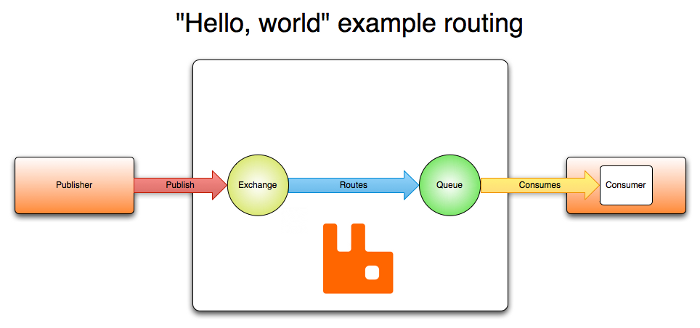
\includegraphics{assets/figures/rabbitmq.png}
    }
    \caption[\gls{AMQP} 0.9.1 Protocol Concepts]{\gls{AMQP} 0.9.1 Protocol Concepts by \cite{rabbitmqexpl}}
    \label{fig:implementation:decisions:rabbitmq}
 \end{figure}

As discussed in \citetitle{rabbitmqexpl}, there are four types of exchanges: 

\begin{itemize}
    \item Direct Exchange: ideal for the unicast routing of messages;
    \item Fanout Exchange: ideal for the broadcast routing of messages;
    \item Topic Exchange: ideal for the multicast routing of messages, queues subscribe to specific routing keys;
    \item Header Exchange: ideal for more flexible unicast routing of messages, queues subscribe to specific message headers;
\end{itemize}

The exchange that better fits the defined requirements is the Topic Exchange.

When working with this protocol and type of exchange, some drawbacks were found:

When dealing with Topic Exchanges a Consumer can only subscribe to one specific routing key or all at once - via \textit{*}- this makes it complex to create routing keys with dynamic values. As an example, lets look at the \textit{Channel} routing key defined in Table~\ref{tab:design:domain:shared_model:routing} of Section~\ref{subsubsec:design:domain:shared_model:routing}. This key defines the single destination of a data unit. For a data unit to have various dynamic service destinations there would be a need to either:

\begin{itemize}
    \item Ensure that every single service subscribes to all relevant combinations of \textit{channel}s possible, deemed impractical;
    \item Duplicate data units, where each copy would be assigned a different channel, deemed inefficient;
\end{itemize}

To tackle this issue, another Message Broker, such as \citetitle{pulsar}, with its own protocol, can be used in the future. This Message Broker answers the drawback describe above by allowing Consumers to subscribe to multiple topics (equivalent to RabbitMQ' routing keys) on the basis of a regular expression (regex), as stated in \citetitle{pulsarmulti}.

The other drawback found is that, according to the \citetitle{rabbitmqprotocol} the routing keys have a max size of 255 bytes. As described in Table~\ref{tab:design:domain:shared_model:routing} of Section~\ref{subsubsec:design:domain:shared_model:routing}, the system currently supports various keys and more keys are expected to be added in the future, meaning that this cap may one day be reached. This limitation lead to the encoding of routing keys in a single character when possible.

\subsection{Usage of Protocol Buffers in Internal Communication}
\label{subsec:implementation:decisions:proto}

This section refers to how messages that flow in the system (via Message Broker) are serialized and deserialized. The common formats used to send structured data across systems are \gls{JSON} and \gls{XML}. This formats, when compared with \citetitle{proto} or \citetitle{thrift}, sacrifice size and de/serialization performance for human readability as stated in \cite{sumaray2012comparison}.

As mentioned before, \textbf{Sensae Console} aims to provide a good developer experience for external costumers that want to expand the solution according to their needs. Due to this, the final decision weighted heavily on formats that were self-documented, e.g. defined by a strict \textit{data schema}, such as \citetitle{proto} and \citetitle{thrift}.

This two technologies, \citetitle{proto} and \citetitle{thrift}, have similar goals and approaches to the problem they try to solve. They both rely on code generation based on a schema of the data structure. The tools related to this formats officially support various languages such as \textit{Java}, \textit{C++}, \textit{C\#}, \textit{Python}, \textit{Go} and others. 

By leveraging this features, creating a basic \gls{SDK} in a new programming language is trivial since serialization, deserialization and data structure is already taken care by the code generation tool.

\citetitle{proto} are a ``language-neutral, platform-neutral, extensible mechanism for serializing structured data''.

\citetitle{thrift}s ``primary goal is to enable efficient and reliable communication across programming languages by abstracting the portions of each language that tend to require the most customization into a common library that is implemented in each language.''

Ultimately \citetitle{proto} were chosen due to better documentation and community support.


\subsection{Database Usage throughout the Solution}
\label{subsec:implementation:decisions:database}

This section refers to how information is stored across the system.

A \gls{DBMS} is a general-purpose software system that facilitates the processes of defining, constructing, manipulating, and sharing data - \citetitle{elmasri2000fundamentals}. \gls{DBMS}s can be categorized according to several criteria, such as the data model, number of users or number of sites. This section focus on the data model, these are some of the data model types, according to \cite{elmasri2000fundamentals}: 

\begin{itemize}
    \item The \textbf{relational data model} represents a database as a collection of tables,
    where each table can be stored as a separate file; 
    \item The \textbf{document-based data model} is based on JSON (Java Script
    Object Notation) and stores the data as documents, which somewhat resemble
    complex objects; 
    \item The \textbf{column-based data model} stores the columns of rows clustered on disk pages for fast access and allow multiple versions of the data;
    \item The \textbf{graph-based data model} stores objects as graph nodes and relationships among objects as directed graph edges;
    \item The \textbf{key-value data model} associates a unique key with each value (which can be a record or object) and provides very fast access to a value given its key.
\end{itemize}

The requirements gathered unveil the need to use three different database' data models throughout the system: (i) relational, (ii) document-based and (iii) column-based data models. The following sections answer why these data models were needed and what technologies were chosen for each of them. A final section unveils an optional solution that was considered but ultimately not pursued.

\subsubsection*{Relational Database Usage}
\label{subsubsec:implementation:decisions:database:relational}

This data model has a wide variety of usage in the industry. Some of the technologies that follow this data model are: (i) \citetitle{mysql}, (ii) \citetitle{postgressql} and (iii) \citetitle{mariadb}.

It is intended for strictly structured data with well defined interrelations. This type of data can be found on most Bounded Contexts described in Section~\ref{subsec:design:domain:bounded_contexts} such as \nameref{subsubsec:design:domain:bounded_contexts:processor}, \nameref{subsubsec:design:domain:bounded_contexts:decoder}, \nameref{subsubsec:design:domain:bounded_contexts:device}, \nameref{subsubsec:design:domain:bounded_contexts:identity}, \nameref{subsubsec:design:domain:bounded_contexts:rule} and the Irrigation Zone/Device concepts of the \nameref{subsubsec:design:domain:bounded_contexts:irrigation} Context.

As such, this data model was adopted for the \textbf{Device Management Database}, \textbf{Data Decoder Database}, \textbf{Data Processor Database}, \textbf{Rule Management Database}, \textbf{Identity Management Database}, \textbf{Smart Irrigation Business Database} and \textbf{Notification Management Database} containers. 

The author had previous contact with all the cited \gls{DBMS}, the decision to use \citetitle{postgressql} was taken based on the fact that, contrary to the other options, \citetitle{postgressql} supports a vast number of Data Types such as \gls{JSON}, Arrays, \gls{UUID}, and Ranges. \citetitle{postgressql}'s data model is an extension of the relation data model, named object-relational data model - \cite{elmasri2000fundamentals}. This data model supports various concepts such as objects, classes and inheritance and therefore can lead to entity models more expressive and close to the business ideas.

\subsubsection*{Document-based Database Usage}
\label{subsubsec:implementation:decisions:database:nosql}

This data model rose from the increasing need to store and analyze unstructured data as stated by \cite{miloslavskaya2016big}.  Citing \cite{elmasri2000fundamentals}, a ``major difference between document-based systems versus object and object-relational systems (...) is that there is no requirement to specify a schema''.

This type of requirements and data resembles the Data Store context described in Section~\ref{subsec:design:system_scopes:data_flow_scope} and Figures~\ref{fig:design:architecture:container:logical:diagram:data_flow} and \ref{fig:design:architecture:container:process:diagram:flow}. This context, intended to mimic a Data Lake\footnote{Massively scalable storage repository that holds a vast amount of raw data in its native format («as is») until it is needed, by \cite{miloslavskaya2016big}}, stores any type of data for future use.

As such, this data model was adopted for the \textbf{Data Store Database} container. 

The only technology considered, and therefore adopted, was \citetitle{mongodb} due to its vast community, excellent documentation and large number of libraries that ease the database management operations. \citetitle{mongodb} also supports replication and sharding according to \cite{elmasri2000fundamentals}, this features is useful once a single node isn't capable of withstanding all data collected while providing fast access to it.

\subsubsection*{Column-based Database Usage}
\label{subsubsec:implementation:decisions:database:time}

This data model is used in applications that require large amounts of data storage, and is commonly named \textit{data warehouses}. According to \cite{dehdouh2015using}, a data warehouse  is ``designed according to a dimensional modelling which has for objective to observe facts through measures, also called indicators, according to the dimensions that represent the analysis axes''. Citing \cite{han2011survey}, this databases ``can maintain high-performance of data analysis and business intelligence processing''.

This features fit the requirements related to storing and reading vast amounts of device measures. As such, it was adopter for the \textbf{Fleet Management Database} and \textbf{Smart Irrigation Data Database} containers.

The author had no previous contact with this type of data model. Some of the technologies related to this concept are: (i) \citetitle{hbase}, (ii) \citetitle{cassandradb}, (iii) \citetitle{influxdb}, (iv) \citetitle{questdb}.

According to \cite{george2011hbase} HBase is a ``distributed, persistent, strictly consistent storage system with near-optimal write and excellent read performance''. This database uses \gls{HDFS} as its file system, and so, it is built on top of Hadoop. 
HBase does not support a structured query language like \gls{SQL}, ``even though it's comprised of a set of standard tables with rows and columns, much like a traditional database'' (\cite{ibm-hbase}).

CassandraDB is a distributed storage system for managing very large amounts of structured data spread out across many commodity servers, while providing highly available service with no single point of failure (\cite{lakshman2010cassandra}).
It was developed internally by Facebook and then later open-sourced to the Apache Foundation. It doesn't support \gls{SQL}.

According to \cite{naqvi2017time}, InfluxDB is an ``open-source schemaless \gls{TSDB} with optional closed-sourced components developed by InfluxData. It is written in Go programming language and it is optimized to handle time series data.'' It provides an SQL-like query language and also defines a new protocol for fast data ingestion (\cite{ilp}).

QuestDB is a relational column-oriented database designed for time series and event data and entitles it self as the ``fastest open source time series database'' (\cite{questdb}).
According to benchmarks (\cite{quest-bench}) preformed using the \gls{TSBS}, \cite{TSBS}, QuestDB ranks as the fastest option in the market.
It has out-of-the-box support for SQL Postgres wire protocol, (thus integrating with \gls{JDBC}), can be easily deployed using a single Docker Image, and also supports the \gls{ILP}.

The type of business this solution is tackling revolves around the capture and analysis of device readings, \gls{IoT}. So the notion of time has to be treated as a first class citizen. The measurements that constitute a time series are ordered on a timeline, which reveals information about underlying patterns.

As stated by \cite{naqvi2017time}, \gls{TSDB} ``can be used to efficiently store sensors and devices' data'' since, ``such technologies are generating large amount of data which is usually time-stamped''.

With this requirements in hand, a column-based data model isn't enough. The technology adopted should also natively support time series to ease data analysis. As such, the \citetitle{hbase} and \citetitle{cassandradb} options were discarded.

Between the two missing options, the author picked \citetitle{questdb} due to better support for \gls{SQL} though \gls{JDBC}. During the research of this two technologies no major downside was found for \citetitle{questdb} when compared to \citetitle{influxdb}.

\subsubsection*{Graph-based Database Usage}
\label{subsubsec:implementation:decisions:database:identity}

Even tho this data model was ultimately not used, the author deemed relevant to mention it.

As stated in the bounded context's section of~\nameref{subsubsec:design:domain:bounded_contexts:identity}, the domains follow a hierarchical structure that can resemble a graph. This context in particular would benefit from a  graph-based database, but this option was not pursued since the author had no previous contact with this family of technologies. Instead \citetitle{postgressql} was used.

\citetitle{postgressql} can represent logical hierarchical structures and concepts using the array data type as the \textit{path} from the root domain to the current domain.

Queries that revolve around graph concepts such as: select parent node, select child nodes, move nodes to a new parent and others, can be preformed efficiently using array operators such as \textbf{\&\&}, \textbf{||} and \textbf{@>}\footnote{taken from PostgresSQL Documentation: \citetitle{postgresarray} \& \citetitle{postgresarrayop}}.

\subsection{Rules Script Engine}
\label{subsec:implementation:decisions:drools}

This section refers to the bounded context of \textbf{Rule Management}. As mentioned before, the purpose of this context is to provide a high-level language that can analyze a stream of Data Units and output alerts base on them. The technology adopted was \citetitle{drools}.

\citetitle{drools} is an open-source rule engine widely used in the industry. The features that stud out from other rule engines were:

\begin{itemize}
    \item Supports for sliding windows of time;
    \item Is also a \gls{CEP} System;
    \item Integrates with the \textit{iot-core} package since it is also written in \textit{Java};
    \item Can be used as a standalone application or an embedded component of another application;
    \item Has an expressive, yet complex, syntax to write rules; 
    \item Can dynamically load rules at runtime.
\end{itemize}

The Section~\ref{subsec:implementation:description:rule} details how one can write rule scenarios.

\subsection{Data Decoders Script Engine}
\label{subsec:implementation:decisions:js}

This section refers to the bounded context of \textbf{Data Decoder}. As mentioned before, this context purpose is to translate inbound Data Units into a format and semantics that the system can understand. The technology adopted was \textit{Javascript}.

\textit{Javascript} is a high level language with an enormous community and is widely used in the industry. Another big reason behind this decision is that a lot of companies producing \gls{IoT} devices provide open-source decoders written in \textit{Javascript}, such as \href{https://github.com/Milesight-IoT/SensorDecoders}{Milesight}
\footnote{\href {https://github.com/Milesight-IoT/SensorDecoders}{github.com/Milesight-IoT/SensorDecoders}}, \href{https://github.com/SensationalSystems}{SensationalSystems}, \href{https://github.com/helium/console-decoders}{Helium}, 
\footnote{\href {https://github.com/helium/console-decoders}{github.com/helium/console-decoders}} and
\footnote{\href {https://github.com/SensationalSystems}{github.com/SensationalSystems}}. This makes it easy and straightforward to integrate new decoders in \textbf{Sensae Console}.

The Section~\ref{subsec:implementation:description:decoder} details how one can write decoders.

\subsection{Containerization of services via Docker}
\label{subsec:implementation:decisions:docker}

This section describes how the final product is packaged using \citetitle{docker}.

As stated in \citetitle{dockerinit}, Docker acts as an intermediary layer between the application to be deployed and the operating system where it will be deployed, ensuring that the developed software has the same behavior regardless of the system. The dependencies of the solution do not have to be present in the system, it is only necessary to install the Docker tool in the \gls{OS}.

This tool thus makes it possible to lower the coupling between the \gls{OS} and the software to be deployed.

With regards for this solution, each container defined in Section~\ref{subsec:design:architecture:containers} is mapped into a docker container.
A container is often compared to a virtual machine running on a hypervisor or
\gls{OS}, but it has a much lower resource consumption, since only the application is run and not not all the processes inherent to an \gls{OS}. Containers execute calls directly to the kernel running on the physical machine and can be seen, unlike virtual machines with their own kernel, as a normal process.

The system is thus represented as a collection of containers that communicate with each other and the outside through standard protocols such as HTTP or AMQP.

The production environment can thus be quickly replicated on another machine in case of a failure disaster or a overwhelming number of interaction with the server.

Details about service containerization can be found in Section~\ref{subsec:implementation:description:docker}.

\subsection{Orchestration of services via Docker Compose}
\label{subsec:implementation:decisions:compose}

This section describes how the final product is orchestrated using Docker Compose.

As stated in the article \citetitle{dockercompose}, ``Compose is a tool for defining and running multi-container Docker applications''. 

Since there is no need to automatically scale the solution it was decided to use a docker compose in production inserted of tools like Kubernetes.

The solution's orchestration is defined in a \textit{YAML} file and then started with a single command. To improve security, only the needed container ports are exposed. To ensure data integrity throughout service disruptions, persistence data is mapped to folder in the \gls{OS}. To ensure an easy management of the environment, configurations are kept in the \gls{OS} and fetched by each container once they start.

The details about the solution orchestration can be found in Section~\ref{subsec:implementation:description:compose}.

\subsection{Usage of Nginx as a web server and reverse proxy}
\label{subsec:implementation:decisions:nginx}

To serve the frontend pages and redirect requests made to backend containers, the following technologies were analyzed:

\begin{itemize}
    \item \citetitle{nginx};
    \item \citetitle{apachehttp};
    \item \citetitle{lighttpd};
\end{itemize}

All of them support the necessary requirements, but some factors lead the author to pick Nginx over the others, the following table, Table~\ref{tab:implementation:decisions:nginx:compare}, describes this criteria.

\begin{table}[H]
    \centering
    \begin{tabular}{@{}clll@{}}
    \toprule
    \textbf{Criteria/Technology} & \textbf{Nginx} & \textbf{Apache HTTP Server} & \textbf{Lighttpd} \\ \midrule
    Resource Consumption      & low  & high      & medium \\ \midrule
    Community Size            & high & very high & medium \\ \midrule
    Familiarity with the tool & high & low       & low    \\ \bottomrule
    \end{tabular}
    \caption{Technologies Comparison - Reverse Proxy Web Server }
    \label{tab:implementation:decisions:nginx:compare}
\end{table}

The details about \citetitle{nginx} configuration can be found in Section~\ref{subsec:implementation:description:nginx}.

\subsection{Usage of Git as a version control system of the project}
\label{subsec:implementation:decisions:git}

\citetitle{git} is a \gls{VCS}. What differentiates it from other
systems such as \citetitle{mercurial} and \citetitle{bitkeeper} is its branching model. It is currently also the most widely used.

\citetitle{github} was the platform used to host the developed code. It offers private repositories with no additional costs. This platform also has other tools such as \textit{Github Issues} and \textit{Github Actions} that ease a developer's workflow. 

A \gls{VCS} is indispensable in software development, this system allows developers to store the history of changes made to the code in an organized manner and simplifies the management of the software by the development team. This system was chosen over others because of the author was experienced with this software.

The development of the entire solution was made in two separated repositories, one for \textit{iot-core} and another for \textbf{Sensae Console}.

The \textit{iot-core} repository had a simple branching model consisting only of a master branch.

There was an extensive use of the branching feature in the repository of \textbf{Sensae Console}, following the model shown in Figure~\ref{fig:implementation:decisions:git:branch}. The author settled for the following: a master branch that matches the deployed version, a development branch where the various features are introduced until a new version is published on the master branch, several branches dedicated to fixing bugs (hotfix) and another several branches that introduce new features and improvements (feature \textit{x}).

\begin{figure}[H]
    \centering
    \resizebox{\columnwidth}{!}
    {
       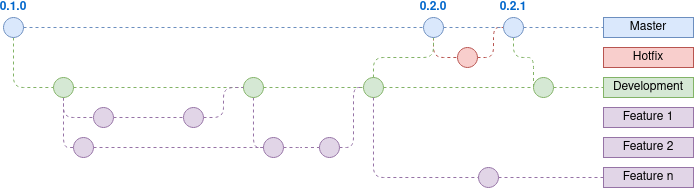
\includegraphics{assets/figures/branching-model.png}
    }
    \caption[Branching Model]{Branching Model}
    \label{fig:implementation:decisions:git:branch}
\end{figure}

This model was adopted since the project was in an initial phase of development, in the future, a branching model with multiple releases, as detailed in Figure~\ref{fig:implementation:decisions:git:branch2}, is preferred. With this model one can release only the altered containers and not the entire system.

\begin{figure}[H]
    \centering
    \resizebox{\columnwidth}{!}
    {
       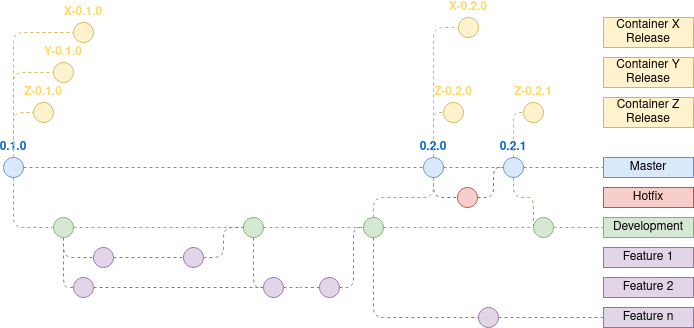
\includegraphics{assets/figures/branching-model-2.png}
    }
    \caption[Future Branching Model]{Future Branching Model}
    \label{fig:implementation:decisions:git:branch2}
\end{figure}

This is useful when using CI/CD pipelines to compile, package and deploy the various containers of the solution. If no changes have been made to \textit{X} Container there is no need to redo all the work previously done with it.

The reason behind the monorepo approach for \textbf{Sensae Console} is that it allows frontend libraries to be shared without publishing somewhere. It is also much easier to keep track of the code in a monorepo since the solution is developed by a single developer.

\subsection{Usage of Github Issues to track issues, bugs and new features}
\label{subsec:implementation:decisions:issues}

As described before, the code is hosted in \citetitle{github}. One of the services that this platform offers is \textit{Github Issues}. This tool helps to track and document the development process alongside with the code.

This tool can be separated into two main views. A view is concerned about what issues, features and bugs are active in the project, Figure~\ref{fig:implementation:decisions:issues:board}, and the other is concerned with the current state of each issue, feature and bug, Figure~\ref{fig:implementation:decisions:issues:project}.

\begin{figure}[H]
    \centering
    \resizebox{\columnwidth}{!}
    {
       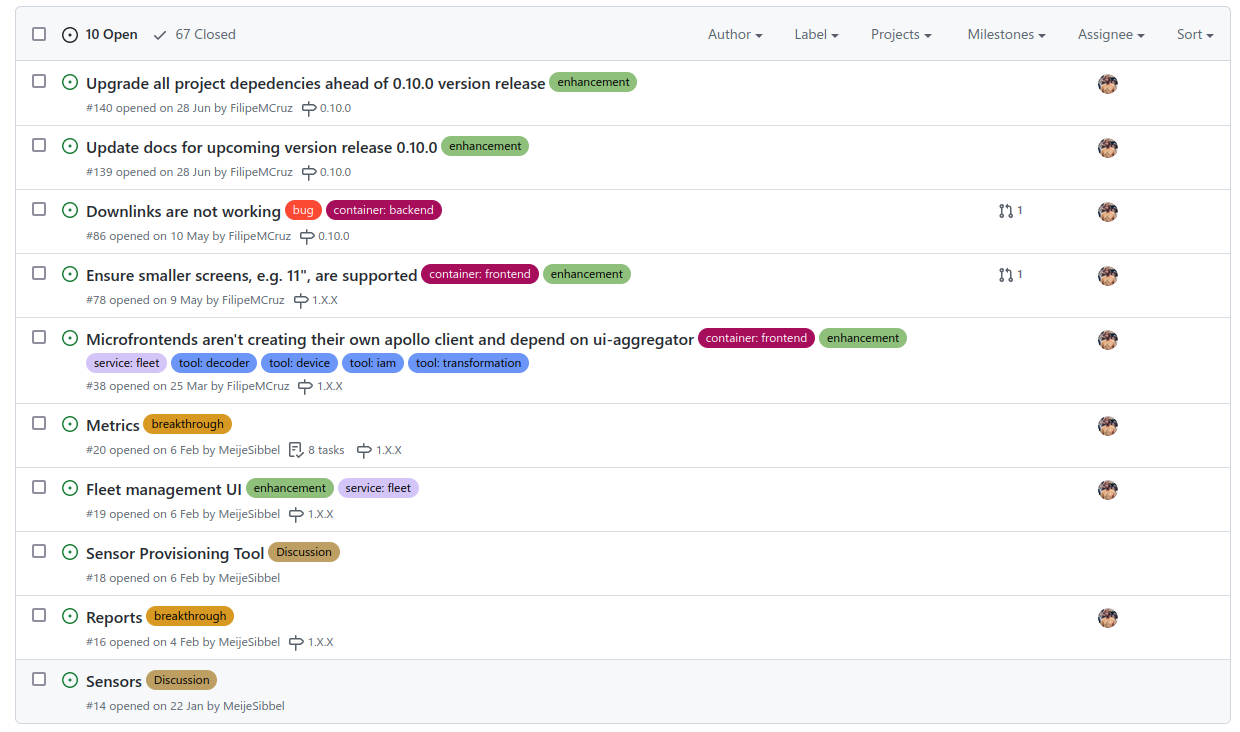
\includegraphics{assets/figures/github-2.png}
    }
    \caption[Github Issues]{Github Issues}
    \label{fig:implementation:decisions:issues:board}
\end{figure}

Each issue has a list of tags that represent its scope and a defined milestone. With this tool, the team members can also discuss issues in depth. 

The issues presented in this page are then tracked in the \textit{project} page - Figure~\ref{fig:implementation:decisions:issues:project}. The author decided to divided the issues into 4 criteria:

\begin{itemize}
    \item \textbf{To Do}: Issues that have been discussed and are to be completed in the near future; 
    \item \textbf{In Progress}: Issues that are currently under development and have an assigned feature branches;
    \item \textbf{Done}: Issues that have been completed and have been integrated in the \textit{master} branch; 
    \item \textbf{Future}: Issues that have been purposed but have no clear deadline.
\end{itemize}

\begin{figure}[H]
    \centering
    \resizebox{\columnwidth}{!}
    {
       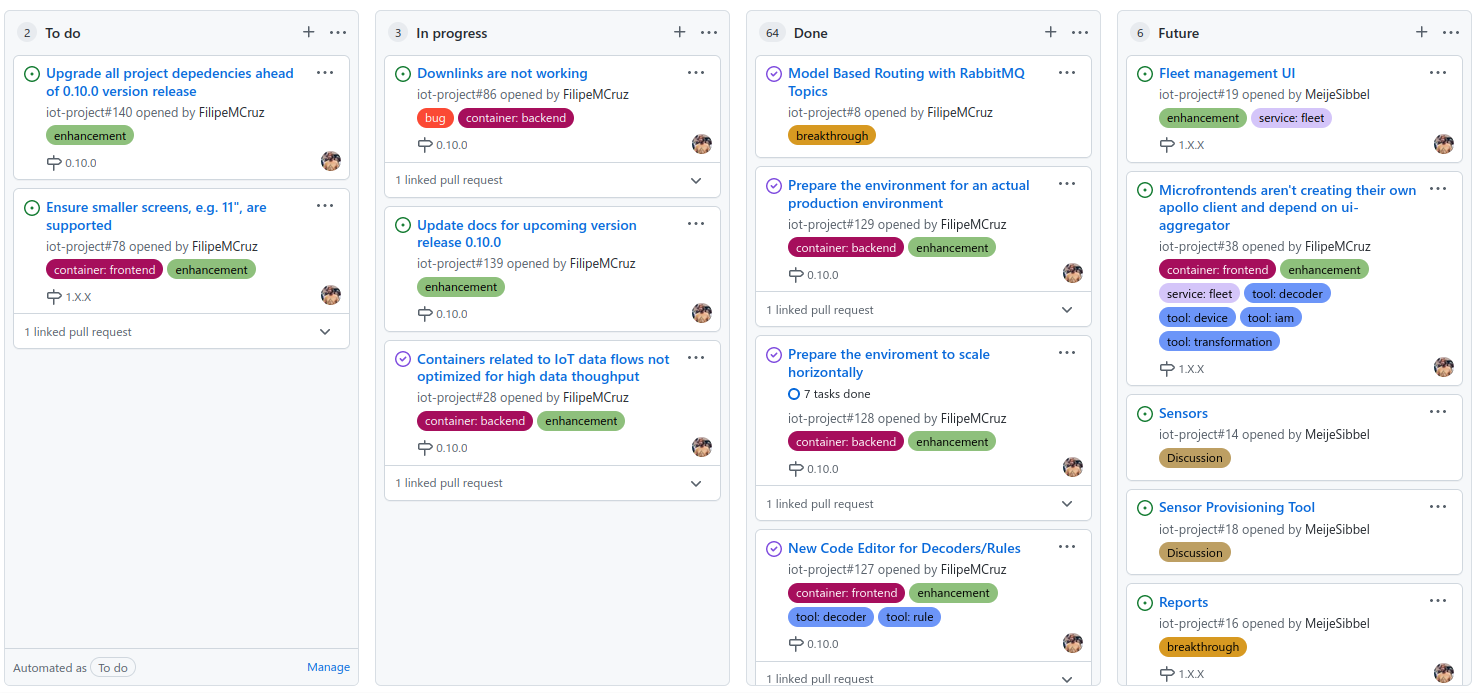
\includegraphics{assets/figures/github.png}
    }
    \caption[Github Issues Project Board]{Github Issues Project Board}
    \label{fig:implementation:decisions:issues:project}
\end{figure}

This view helps to define a simple project roadmap and track the overall state of issues, bugs and features in the project.

\subsection{Usage of Github Actions for CI/CD}
\label{subsec:implementation:decisions:actions}

Since the code is hosted in \textit{Github}, it was decided to leverage the CI/CD features of the platform. \textit{Github Actions} purpose is to automate software workflows via CI/CD.

According to \cite{cicd}, the term CI/CD represents a method to delivering applications to clients by introducing automation into the development states.
It is divided into three concepts:

\begin{itemize}
    \item \textbf{Continuous Integration}: new versions of the project are regularly submitted, tested and merged into the current project;
    \item \textbf{Continuous Delivery}: new versions of the project are automatically archived in a repository where they can then be deployed to a production environment;
    \item \textbf{Continuous Deployment}: new versions of the project are automatically deployed to a production environment.
\end{itemize}

The \textit{iot-core} package is archived in a repository so that it can then be integrated in the backend containers of \textbf{Sensae Console}, and possibly in other projects. To do so, the team uses \textit{Github Actions}. This tool's behavior is defined in a YAML file, presented in the Code Sample~\ref{code:implementation:decisions:actions:iotcore}.

\begin{lstlisting}[style=yaml, caption=Configuration File for \textit{iot-core} Continuous Delivery, label={code:implementation:decisions:actions:iotcore}]
name: IoT Core - Continuous Delivery to maven central
on:
  push:
    tags:        
      - '**'
      - '*'
jobs:
  build:
    runs-on: ubuntu-latest
    steps:
      - uses: actions/checkout@v2
      - name: Set up Maven Central Repository
        uses: actions/setup-java@v1
        with:
          java-version: 17
          server-id: ossrh
          server-username: MAVEN_USERNAME
          server-password: MAVEN_PASSWORD
          gpg-private-key: ${{ secrets.MAVEN_GPG_PRIVATE_KEY }}
          gpg-passphrase: MAVEN_GPG_PASSPHRASE
      - name: Deploy with Maven
        run: mvn -B clean deploy -Pci-cd
        env:
          MAVEN_USERNAME: ${{ secrets.OSSRH_USERNAME }}
          MAVEN_PASSWORD: ${{ secrets.OSSRH_TOKEN }}
          MAVEN_GPG_PASSPHRASE: ${{ secrets.MAVEN_GPG_PASSPHRASE }}
\end{lstlisting}

As we can see in lines \textbf{2} to \textbf{6}, this action is triggered every time a new git tag is pushed to the repository.
This action then proceeds to download and setup java and maven - lines \textbf{12} to \textbf{20}. Finally it runs a maven command to deploy the new version to the artifact repository - lines \textbf{21} to \textbf{26}. 

The \textbf{Sensae Console} has an action to deal with Continuous Integration - Code Sample~\ref{code:implementation:decisions:actions:cisensae}, where changes made to the software are tested.

\begin{lstlisting}[style=yaml, caption=Configuration File for \textbf{Sensae Console} Continuous Integration, label={code:implementation:decisions:actions:cisensae}]
name: Sensae Console - Continuous Integration - Test changes
on:
  push:
    branches:
      - master
      - dev
jobs:
  test:
    runs-on: ubuntu-latest
    steps:
      - uses: actions/checkout@v3
      - name: Set up JDK 17
        uses: actions/setup-java@v3
        with:
          java-version: "17"
          distribution: "adopt"
      - name: Set up Node 16
        uses: actions/setup-node@v3
        with:
          node-version: 16
      - name: Test Suite
        run: |
          ./project/scripts/run-tests.sh "${{ secrets.mapbox_token }}" "${{ secrets.microsoft_audience }}" "${{ secrets.google_audience }}" "${{ secrets.admin_email }}"

\end{lstlisting}

As we can see in lines \textbf{2} to \textbf{6}, this action is triggered every time a new commit is push to the \textit{dev} and \textit{master} branches.
This action then proceeds to download and setup java and maven - lines \textbf{10} to \textbf{16}, and then node and npm - lines \textbf{17} to \textbf{20}. Finally it runs a script that tests the solution - line \textbf{23}. The script requires the displayed secrets to run some tests, this tests will be discussed in the \nameref{sec:implementation:testing} Section.

The mentioned script has the following structure - Code Sample~\ref{code:implementation:decisions:actions:testscript}.

\begin{lstlisting}[language=bash, style=bash, caption=Sensae Console Test Suite Script, label={code:implementation:decisions:actions:testscript}]
#!/bin/bash
set -eo pipefail

ROOT_DIR=$(git rev-parse --show-toplevel)

cd "$ROOT_DIR"/project || exit

./scripts/generate-test-config.sh "$@"

docker-compose -f docker-compose.build.yml build

rm --f -- reports/backend-test-pass.log
rm --f -- reports/backend-test-fail.log

cd backend-services || exit

ls -I data-relayer | xargs -I % sh -c 'cd % && mvn test && \
    echo % >> ../../reports/backend-test-pass.log || \
    echo % >> ../../reports/backend-test-fail.log'

test ! -f ../reports/backend-test-fail.log

cd ../frontend-services || exit

npm install
npm run test-all

./../scripts/build-images.sh

docker-compose -f ../docker-compose.test.yml up -d --build

sleep 60

npm run e2e-all

docker-compose -f ../docker-compose.test.yml down    
\end{lstlisting}

This script first intent is to defined a basic environment where tests can be run.
The flag \textit{set -eo pipefail} ensures that if any command fails the script will terminate and exit with an error.
It runs the following steps:

\begin{itemize}
    \item Generate configurations - line \textbf{8} - to run every test according to the secrets provided by the github action presented at Listing~\ref{code:implementation:decisions:actions:cisensae},
    \item Build the database containers - line \textbf{10}. The file \textit{docker-compose.build.yml} references all the solution's databases that need a custom build due to their predefined schema;
    \item Run the command \textit{mvn test} for all backend containers and store the results of each container's test in a file - lines \textbf{17} to \textbf{19};
    \item Checks if any container didn't pass the tests - line \textbf{15};
    \item Run tests related to the frontend at lines \textbf{23} to \textbf{26}. The script mentioned as \textit{test-all} is: \textit{nx run-many --all --target=test}. This script runs all unit tests of both frontend libraries and apps using \citetitle{nx}, as mentioned in \ref{subsubsec:implementation:decisions:frontend:nx} Section;
    \item Build and start an environment similar to the production one - lines \textbf{28} to \textbf{32};
    \item Preform end to end tests against the test environment - \textbf{34}. The script mentioned as \textit{e2e-all} is: \textit{nx run-many --all --target=e2e --parallel=1}. This script runs all end-to-end tests of the frontend apps using \citetitle{nx}, as mentioned in \ref{subsubsec:implementation:decisions:frontend:nx} Section;
    \item Shutdown the test environment.
\end{itemize}

\subsection{Usage of Maven Repository to host Open-Source Code}
\label{subsec:implementation:decisions:maven}

As stated in the previous section \textit{iot-core} is delivered to an artifact repository. Since the intent of this package is to be used by any one interested on integrating his/her tool with \textbf{Sensae Console}, the artifact repository has to be publicly available. 

The Maven Central repository was the chosen one, since the \textit{maven} and \textit{gradle} tools use it, by default, to fetch dependencies.

According to the article \citetitle{centralreq} by \cite{centralreq}, to publish an artifact to maven central, a couple of additions have to be made in the \textit{pom.xml} of the project namely: (i) Supply Javadoc and Sources, (ii) Provide Files Checksums, (iii) Sign Files with GPG/PGP, (iv) Sufficient Metadata, (v) Correct Coordinates, (vi) Project Name, Description and URL, (vii) License Information, (vii) Developer Information, (viii) SCM Information.

In the Appendix~\ref{AppendixE} Appendix the full \textit{pom.xml} is presented.

\section{Technical Description}
\label{sec:implementation:description}

This section guides the reader though \textbf{Sensae Console} with a technical description of the various elements that are exposed to the final costumers and platform managers.

It describes the following topics:

\begin{itemize}
    \item \nameref{subsec:implementation:description:ui};
    \item \nameref{subsec:implementation:description:maps};
    \item \nameref{subsec:implementation:description:api};
    \item \nameref{subsec:implementation:description:ingestion};
    \item \nameref{subsec:implementation:description:rule};
    \item \nameref{subsec:implementation:description:decoder};
    \item \nameref{subsec:implementation:description:database};
    \item \nameref{subsec:implementation:description:docker};
    \item \nameref{subsec:implementation:description:compose};
    \item \nameref{subsec:implementation:description:nginx};
    \item \nameref{subsec:implementation:description:config};
    \item \nameref{subsec:implementation:description:services};
    \item \nameref{subsec:implementation:description:sensor};
\end{itemize}

\subsection{Sensae Console UI}
\label{subsec:implementation:description:ui}

In this subsection the \gls{UI} is presented.

The Figure~\ref{fig:implementation:description:ui:home} represents the main layout for any user. It is comprised of a toolbar with a section for \textbf{Service Pages}, another for \textbf{Configuration Pages} and a final one for authentication purposes.

\begin{figure}[H]
    \centering
    \resizebox{\columnwidth}{!}
    {
       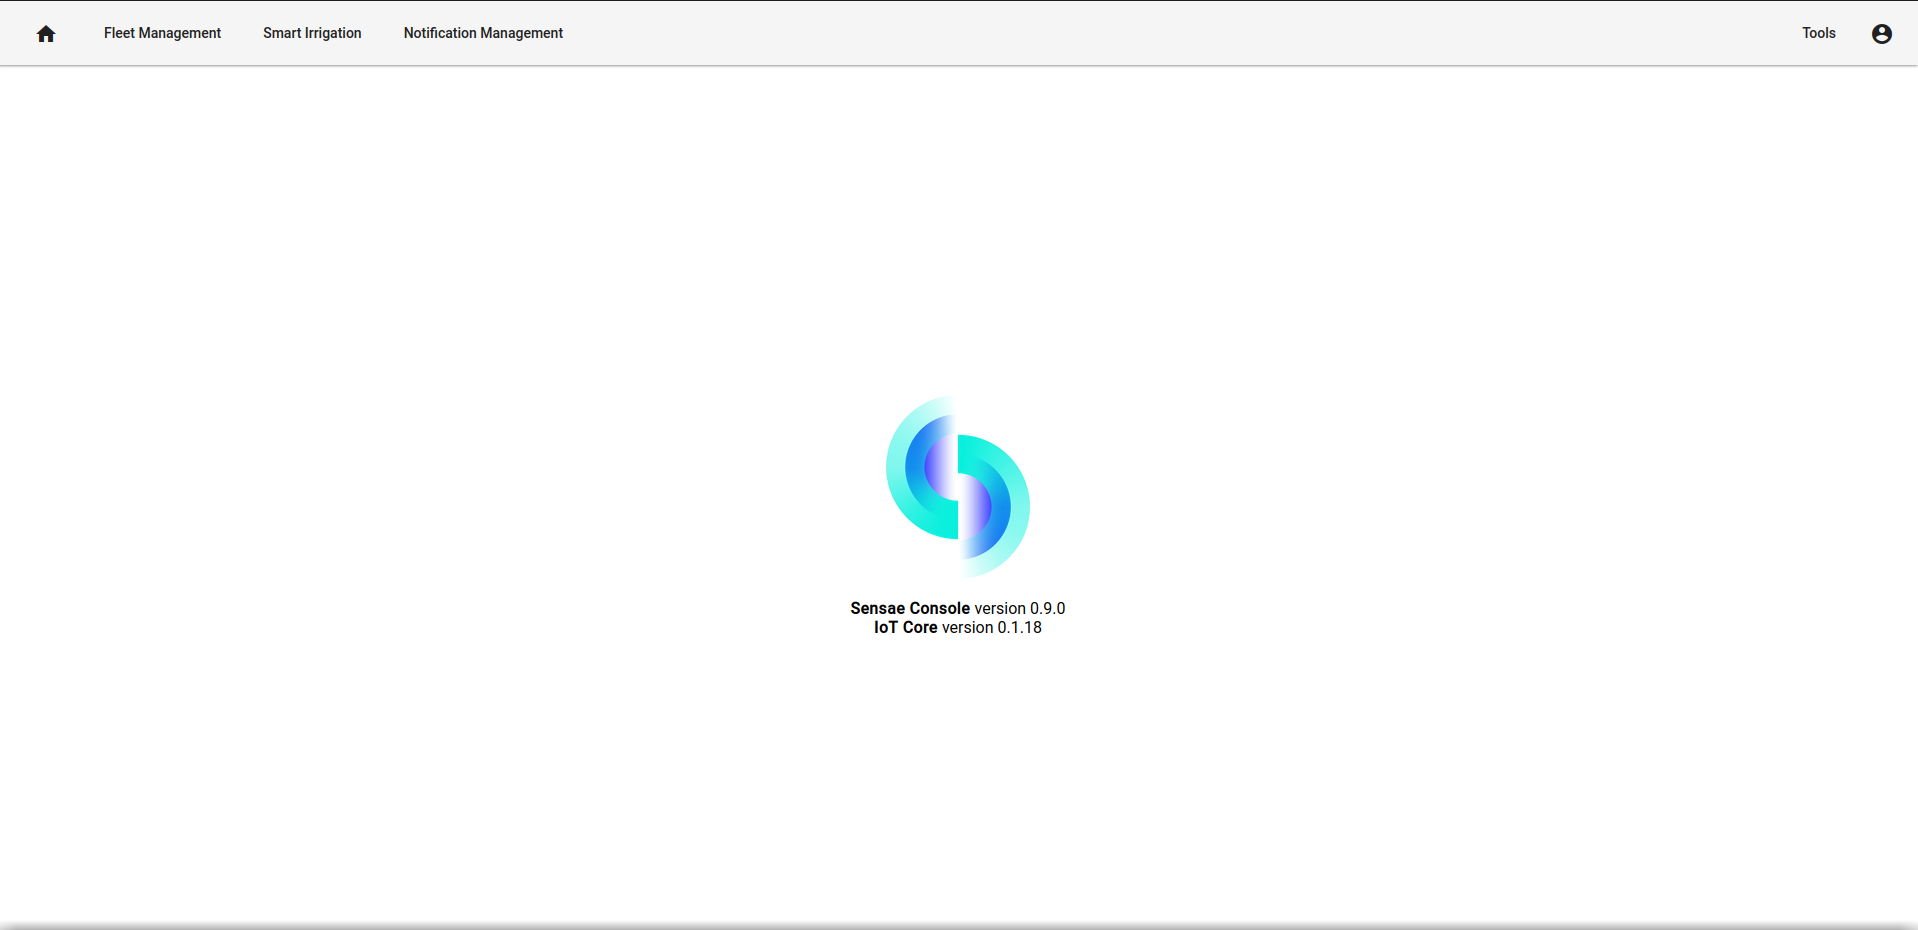
\includegraphics{assets/figures/ui/home.png}
    }
    \caption[Sensae Console Home Page]{Sensae Console Home Page}
    \label{fig:implementation:description:ui:home}
\end{figure}

From this page, if the user has sufficient permissions, one can access services pages, as an example the \textbf{Smart Irrigation Page} is displayed in Figure~\ref{fig:implementation:description:ui:smartirrigation}.
This page presents a map where the user can see, search and create irrigation zones. Device measures are updated in real time via \textit{Websocket}s. The user can also see the irrigation zone details after clicking on it. From there it's possible to open/close valves an see the history of measures of each device. 

\begin{figure}[H]
    \centering
    \resizebox{\columnwidth}{!}
    {
       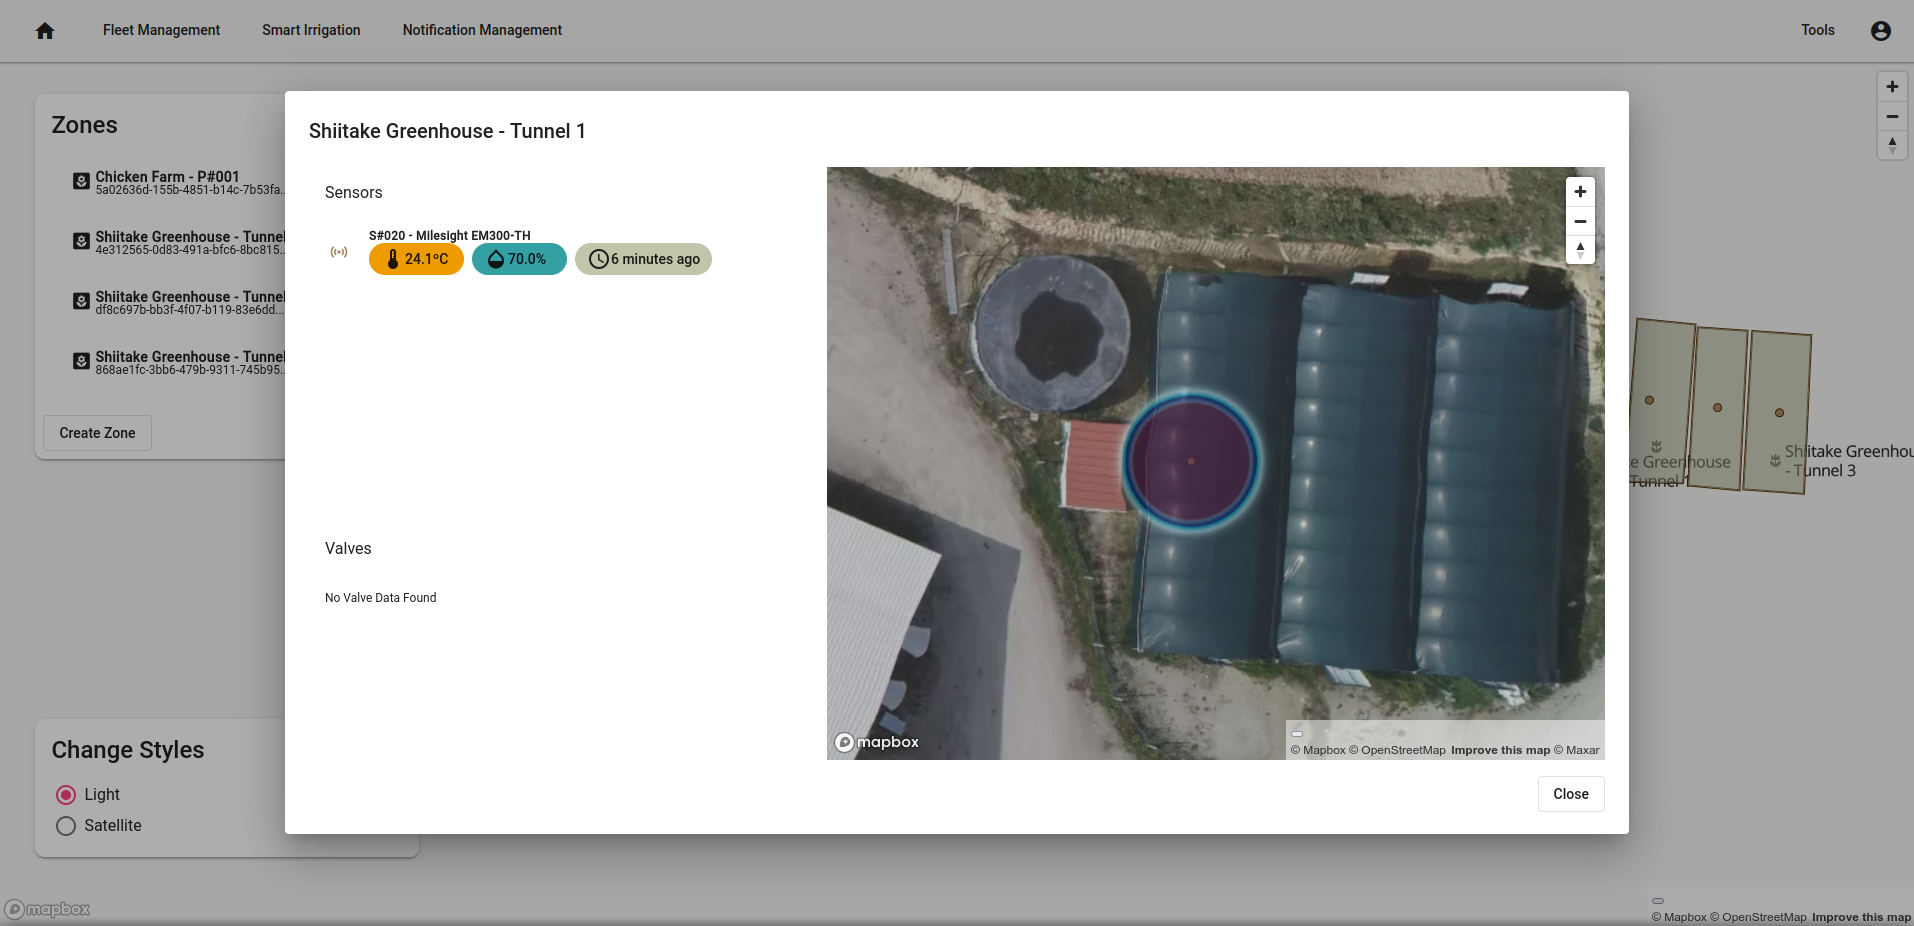
\includegraphics{assets/figures/ui/smart-irrigation.png}
    }
    \caption[Sensae Console Smart Irrigation Page]{Sensae Console Smart Irrigation Page}
    \label{fig:implementation:description:ui:smartirrigation}
\end{figure}

From the home page the user can also access configuration pages, as an example the \textbf{Device Management Page} is displayed in Figure~\ref{fig:implementation:description:ui:device}.

\begin{figure}[H]
    \centering
    \resizebox{\columnwidth}{!}
    {
       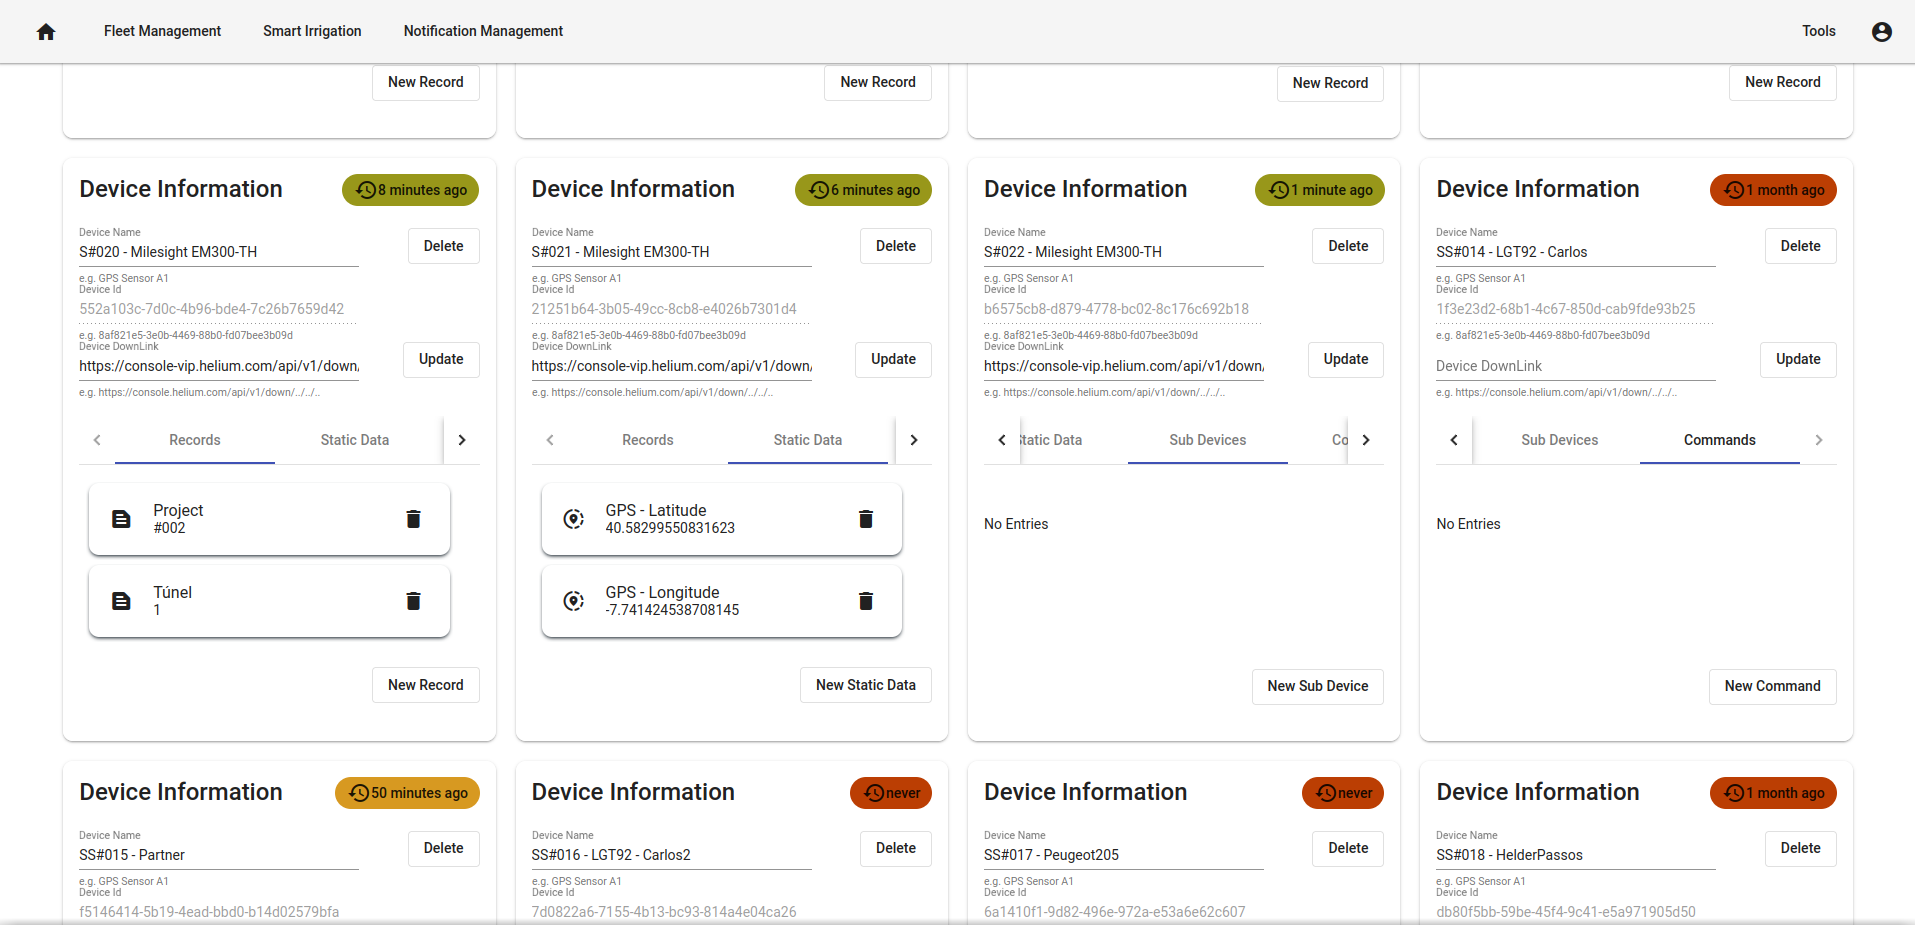
\includegraphics{assets/figures/ui/device-management.png}
    }
    \caption[Sensae Console Device Management Page]{Sensae Console Device Management Page}
    \label{fig:implementation:description:ui:device}
\end{figure}

In this page the user can see when was the last time the device interacted with the platform, create and delete devices and edit the details of each device according to the model presented in Section\nameref{subsubsec:design:domain:bounded_contexts:device} of the \textit{Bounded Contexts}.

Other relevant pages are presented in the Appendix~\ref{AppendixD}.

\subsection{Sensae Console Custom Maps}
\label{subsec:implementation:description:maps}

This section describes how custom maps where built to fit the solution needs. Some costumers facilities were not present in the satellite view of \citetitle{googlemaps} or \citetitle{mapbox}. A custom map, with the missing facilities, was built using satellite images taken with a drone. The images where processed with \citetitle{arcgis} and transformed in \textit{.tiff} files that could be incorporated in the basic satellite layer of \citetitle{mapbox}.

The following image, Figure~\ref{fig:implementation:description:maps:irrig} presents the new map with the costumer facilities in a greener tone than the rest of the map. This map was used to display three greenhouses and a chicken farm that belong to a costumer. This map is currently in use by the Smart Irrigation Service.

\begin{figure}[H]
    \centering
    \resizebox{\columnwidth}{!}
    {
       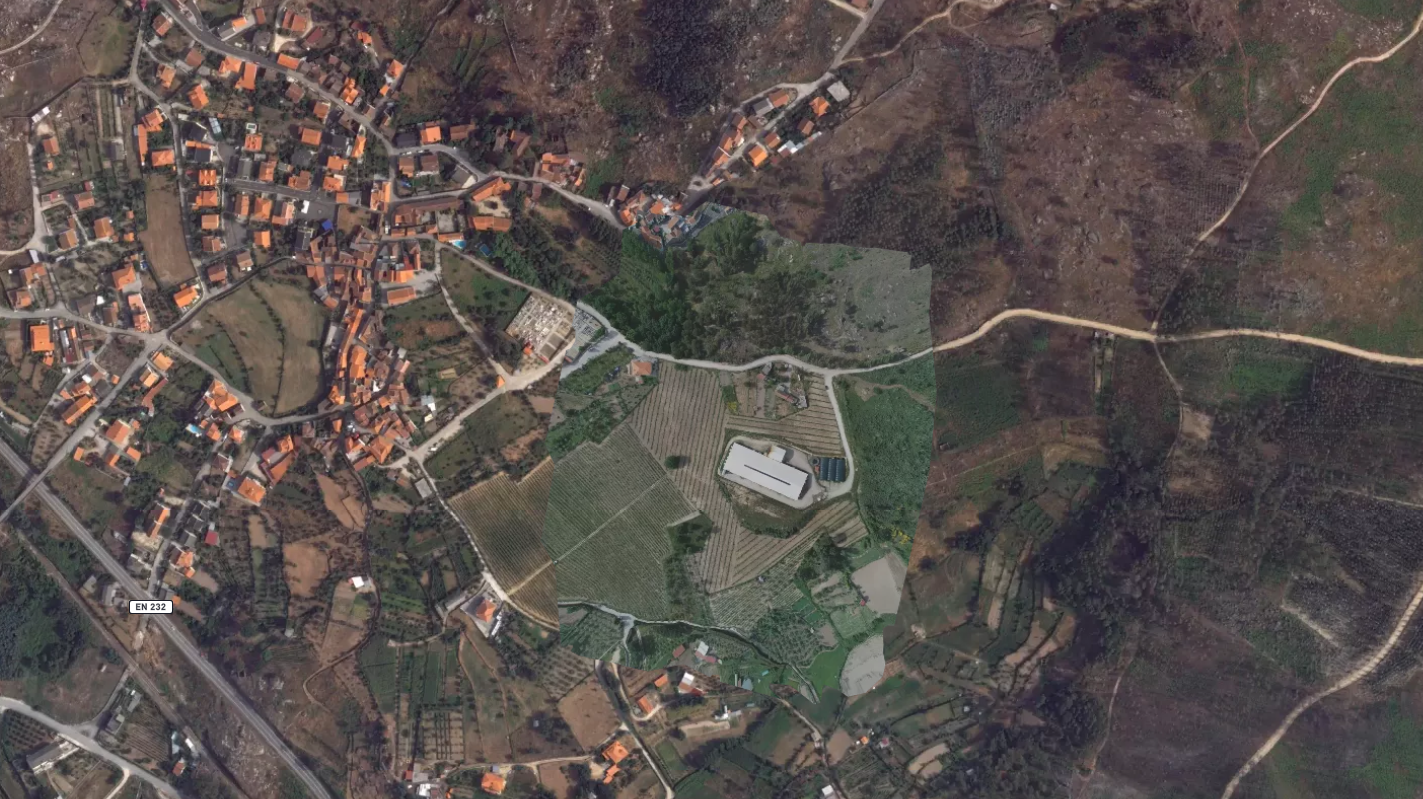
\includegraphics{assets/figures/maps/custom-map.png}
    }
    \caption[Custom Map - Smart Irrigation]{Custom Map - Smart Irrigation}
    \label{fig:implementation:description:maps:irrig}
\end{figure}

The road trajectory mismatch present in the map could be reduced by taking pictures from more angles. \citetitle{arcgis} would create better model with a wider pool of information.

\subsection{Sensae Console Backend API}
\label{subsec:implementation:description:api}

The \textbf{Sensae Console} \gls{API} is served as a \citetitle{graphql} \gls{API}, one for each service/configuration context. This \gls{API} is described with a schema.

As an example the Smart Irrigation API is presented in the Code Sample~\ref{code:implementation:description:api:irrigation}. 

\begin{lstlisting}[caption=Smart Irrigation API Schema, label={code:implementation:description:api:irrigation}]
type Subscription {
    data(filters: LiveDataFilter, Authorization: String) : SensorData
}

type Query {
    history(filters: HistoryQueryFilters) : [SensorDataHistory]
    fetchIrrigationZones : [IrrigationZone]
    fetchLatestData(filters: LatestDataQueryFilters): [SensorData]
}

type Mutation {
    createIrrigationZone(instructions: CreateIrrigationZoneCommand) : IrrigationZone
    updateIrrigationZone(instructions: UpdateIrrigationZoneCommand) : IrrigationZone
    deleteIrrigationZone(instructions: DeleteIrrigationZoneCommand) : IrrigationZone
    switchValve(instructions: ValvesToSwitch): Boolean
}        
\end{lstlisting}

From the observation of the code sample one can see that:

\begin{itemize}
    \item The \textit{data} function serves new \textit{SensorData} in real-time according to the filters provided in the \textit{filters} parameter;
    \item The textit{data} function uses \textit{Websocket} to operate as a full duplex communication channel. This spec, contrary to the HTTP spec does not account for HTTP Headers, as such the \gls{JWT} that provides the user authentication details has to be sent as a normal parameter and not as an Authorization HTTP Header.
    \item  There are three query type functions. One to fetch the history regarding Irrigation Zones or Devices over a time span. One to fetch the Irrigation Zones. And the last one to fetch the latest data of each device;
    \item There are four mutations, each corresponding to the use cases referenced in \textbf{***TODO***}.
\end{itemize}

\subsection{Sensae Console Data Ingestion Endpoint}
\label{subsec:implementation:description:ingestion}

The Data Ingestion Endpoint refers to how device data is sent to \textbf{Sensae Console}.

The endpoint corresponds to an HTTP POST verb with the following \gls{URL} schema:

\begin{verbatim}
    https://<ip>:<port>/sensor-data/{channel}/{infoType}/{deviceType}
\end{verbatim}

The endpoint collects the request body and then forwards it with the appropriate routing keys.

The routing keys are created according to the Table~\ref{tab:design:domain:shared_model:routing}. The \textit{infoType} can have two values: ENCODED or DECODED. Depending on this value the message is routed to \textit{Data Decoder Flow} or \textit{Data Processor Flow} as described in Figure~\ref{fig:design:architecture:container:logical:diagram:data_flow}.

The \textit{channel} parameter indicates the final service that it is destine to: \textit{fleet} for Fleet Management Service or \textit{irrigation} for Smart Irrigation Service. If another value is given the message is not routed to any service.

Finally, to ensure that the requests to this endpoint are trustworthy, a secret has to be sent in the Authorization HTTP Header. This secret is defined as a configuration of the \textbf{Sensae Console}, discussed in Section~\ref{subsec:implementation:description:config}.

\subsection{Sensae Console Rule Engine}
\label{subsec:implementation:description:rule}

The rule engine can be access from the \textbf{Rule Management Page} of the UI and, as stated in \nameref{subsubsec:design:domain:bounded_contexts:rule} Bounded Context, it provides a high-level language that can be used to detect anomalies in \textbf{Data Unit}s and turn them into \textbf{Alert}s.

Valid \textbf{Data Unit}s are captured by \textbf{Alert dispatcher Backend} and the inserted in the Rule Engine.

As stated in \nameref{subsec:implementation:decisions:drools}, the rule engine used was \citetitle{drools}. To write rules for \textbf{Sensae Console} one must follow several guidelines.

A \citetitle{drools} rule is composed by conditions, actions and facts.

Facts are inserted in the rule engine. If a fact or group of facts match a condition (\textit{when} section), an action is triggered (\textit{then} section).

The rule engine, is tailored to managers or developers and not for final clients since it can be hard to create meaningfully rules without side effects.

To clarify the guidelines the following Code Samples~\ref{code:implementation:description:rule:sample1}, ~\ref{code:implementation:description:rule:sample2} and \ref{code:implementation:description:rule:sample3} are presented.

The first Code Sample presents the beginning of the rule scenario, where imports and new Facts are created.

\begin{lstlisting}[style=drools, caption=Rule Scenario Example - Part 1, label={code:implementation:description:rule:sample1}]
package rules.project.two;

import pt.sharespot.iot.core.data.model.data.DataUnitReadingsDTO;
import pt.sharespot.iot.core.data.model.DataUnitDTO;
import pt.sharespot.iot.core.data.model.device.records. DeviceRecordEntryDTO;
import pt.sharespot.iot.core.data.model.properties.PropertyName;
import pt.sharespot.iot.core.alert.model.AlertBuilder;
import pt.sharespot.iot.core.alert.model.CorrelationDataBuilder;
import pt.sharespot.iot.core.alert.model.AlertLevel;
import java.util.List;
import java.util.UUID;

global pt.sharespot.iot.core.alert.model.AlertDispatcherService dispatcher;

dialect "mvel"

declare StoveSensor
    @role( event )
    deviceId : UUID
end

declare StoveSensorData
    @role( event )
    deviceId : UUID
    dataId : UUID
    temperature : Float
    humidity : Float
end
\end{lstlisting}

As we can see, from line \textbf{3} to \textbf{9}, classes from \textit{iot-core} are imported into the scenario.
At line \textbf{13} the interface that defines how an alert can be sent is imported for later use.
From line \textbf{17} to \textbf{28} two facts are declared, this can later be used as simple \textit{Java} POJOs. A fact defined with the \textit{event} role means that it occurred at a specific time (upon creation) and can be used for \gls{CEP}. 

The following code sample presents a simple rule to store \textit{StoveSensorData} facts in the working memory of \citetitle{drools}. 

\begin{lstlisting}[style=drools, caption=Rule Scenario Example - Part 2, label={code:implementation:description:rule:sample2}] 
rule "Collect stove sensor data that belongs to Project #002"
    when
        $d : DataUnitDTO(
            getSensorData()
            .hasProperty(PropertyName.AIR_HUMIDITY_RELATIVE_PERCENTAGE),
            getSensorData()
            .hasProperty(PropertyName.TEMPERATURE)
        )
        exists DeviceRecordEntryDTO(
            label == "Project" && content == "#002"
        ) from $d.device.records
        not(StoveSensorData(dataId == $d.dataId))
    then
        StoveSensorData reading = new StoveSensorData();
        reading.setDeviceId($d.device.id);
        reading.setDataId($d.dataId);
        reading.setTemperature($d.getSensorData().temperature.celsius);
        reading.setHumidity($d.getSensorData().airHumidity .relativePercentage);
        insert(reading)
end
\end{lstlisting}

As we can see this rule is composed by two sections, the \textit{when} and \textit{then} sections. In the \textit{when} the following conditions are defined:

\begin{itemize}
    \item The captured DataUnitDTO has AIR HUMIDITY RELATIVE PERCENTAGE and TEMPERATURE measures - lines \textbf{3} to \textbf{8};
    \item The capture DataUnitDTO has a record with a "Project" label and "\#002" content - lines \textbf{9} to \textbf{11};
    \item The DataUnitDTO is not a duplicate fact in the working memory - line \textbf{12}.
\end{itemize}

Once this conditions are meet a \textit{StoveSensorData} is created with all the needed information and then inserted into the working memory - lines \textbf{14} to \textbf{19}.

The following code sample presents a simple rule to dispatch an \textbf{Alert} after some conditions are meet. 

\begin{lstlisting}[style=drools, caption=Rule Scenario Example - Part 3, label={code:implementation:description:rule:sample3}]
rule "Dispatch Stove Alarm - Dry Soil Scenario - Project #002"
    when
        $s : StoveSensorData(temperature > 26, humidity < 50)
        not(StoveSensorData(this != $s,
                temperature < 26,
                humidity > 50,
                this after[0s,11m] $s)
        )
    then 
        dispatcher.publish(AlertBuilder.create()
                            .setCategory("irrigation")
                            .setSubCategory("drySoilDetected")
                            .setDescription("Project #002 - Device "+ $s.deviceId +" detected low humidity/high temperature")
                            .setLevel(AlertLevel.ADVISORY)
                            .setContext(CorrelationDataBuilder.create()
                                .setDeviceIds($s.deviceId)
                                .setOther("Project #002")
                                .build())
                            .build());
end
\end{lstlisting}

As we can see this rule matches when the same device reports measures of air humidity higher than 50\% and temperature lower then 26 ºC for more than 11 minutes.

Once it matches an Alert is dispatched using the referenced dispatcher in Code Sample~\ref{code:implementation:description:rule:sample1}. The Alert can be created using the builder pattern.

An Alert closely resembles a Notification from the \nameref{subsubsec:design:domain:bounded_contexts:notification} Bounded Context. It also has a category (line \textbf{13}), a sub category (line \textbf{14}), a severity level (line \textbf{16}), a description (line \textbf{15}) and a notification context (lines \textbf{17} to \textbf{20}).

For an \textbf{Alert} to be sent at least the category and sub category parameters have to be set. By default the \textbf{INFORMATION} severity level is used.

In order for services to act upon a received \textbf{Alert}, it has to be associated with a \textit{DeviceId} (this association helps services like \textbf{Smart Irrigation} to know what Valve must be turned on or off), a \textit{DataId} or \textit{Other}.

An \textbf{Alert} is later transformed and store as a Notification, the \textit{DeviceId}s associated to it are used to determine what domains will have access to the Notification. If no \textit{DeviceId}s are associated only the root domain will have access to it.

\subsection{Sensae Console Data Decoders}
\label{subsec:implementation:description:decoder}

As mentioned in the \nameref{subsubsec:design:domain:bounded_contexts:decoder} Bounded Context Section, \textbf{Data decoder}'s purpose is to provide a flexible option to transform inbound data units into something that the system understands.

This happens when a \textbf{Data Unit} has a routing key with the ENCODED info type.

There are certain guidelines to follow in order to create a decoder:

\begin{itemize}
    \item Has to be written in vanilla \textit{javascript};
    \item Has to have an \textit{entry} function with the following signature \textit{function convert(dataUnit)};
    \item Can't import any node function, npm package or reference other scripts.
\end{itemize}

As an example, the Code Sample~\ref{code:implementation:description:decoder:em300th} presents the decoder for the device type EM500-TH\footnote{https://www.milesight-iot.com/lorawan/sensor/em300-th}.

\begin{lstlisting}[style=javascript, caption=EM300-TH Data Decoder Example, label={code:implementation:description:decoder:em300th}] 
const decodePayload = (payload, port) =>
    ({"0": decoder(base64ToHex(payload), port)});

const base64ToHex = (() => {
    const values = [], output = [];

    return function base64ToHex(txt) {
        if (output.length <= 0) populateLookups();
        const result = [];
        let v1, v2, v3, v4;
        for (let i = 0, len = txt.length; i < len; i += 4) {
            v1 = values[txt.charCodeAt(i)];
            v2 = values[txt.charCodeAt(i + 1)];
            v3 = values[txt.charCodeAt(i + 2)];
            v4 = values[txt.charCodeAt(i + 3)];
            result.push(
                parseInt(output[(v1 << 2) | (v2 >> 4)], 16),
                parseInt(output[((v2 & 15) << 4) | (v3 >> 2)], 16),
                parseInt(output[((v3 & 3) << 6) | v4], 16)
            );
        }
        if (v4 === 64) result.splice(v3 === 64 ? -2 : -1);
        return result;
    };
    function populateLookups() {
        const keys =
            "ABCDEFGHIJKLMNOPQRSTUVWXYZabcdefghijkl mnopqrstuvwxyz0123456789+/=";
        for (let i = 0; i < 256; i++) {
            output.push(("0" + i.toString(16)).slice(-2));
            values.push(0);
        }
        for (let i = 0; i < 65; i++) values[keys.charCodeAt(i)] = i;
    }
})();

function decoder(bytes, port) {
    let decoded = {}, temperature = {}, airHumidity = {}, battery = {};
    for (let i = 0; i < bytes.length;) {
        let channel_id = bytes[i++];
        let channel_type = bytes[i++];
        if (channel_id === 0x01 && channel_type === 0x75) {
            decoded.battery = battery;
            battery.percentage = bytes[i];
            i += 1;
        } else if (channel_id === 0x03 && channel_type === 0x67) {
            decoded.temperature = temperature;
            temperature.celsius = readInt16LE(bytes.slice(i,i+2))/10;
            i += 2;
        } else if (channel_id === 0x04 && channel_type === 0x68) {
            decoded.airHumidity = airHumidity;
            airHumidity.relativePercentage = bytes[i] / 2;
            i += 1;
        } else {
            break;
        }
    }
    return decoded;
}
const readUInt16LE = bytes => (bytes[1] << 8) + bytes[0] & 0xffff;

function readInt16LE(bytes) {
    let ref = readUInt16LE(bytes);
    return ref > 0x7fff ? ref - 0x10000 : ref;
}
const convert = dataUnit => ({
    dataId: dataUnit.uuid,
    reportedAt: dataUnit.reported_at,
    device: {
        id: dataUnit.id,
        name: dataUnit.name,
        downlink: dataUnit.downlink_url,
    },
    measures: decodePayload(dataUnit.payload, dataUnit.port),
});
\end{lstlisting}

As we can see, this code sample decodes an EM300-TH \textbf{Data Unit}. The function \textit{convert} is the one mentioned in the guidelines, it assigns values such as \textit{id}, \textit{name}, \textit{reported\_at}, \textit{downlink\_url}, \textit{uuid} to its correct place and calls the function \textit{decodePayload} to gather the device measures. The \textit{decodePayload} stores every measure in the \textit{controller} key - value \textit{0}. The function \textit{base64ToHex} is the function that reads a Base 64 string and transforms it into a Hex Array - to reduce bandwidth the device normally encodes and sends data as a base 64 string. The function \textit{decoder}, \textit{readInt16LE} and \textit{readUInt16LE} were adapted from the TTN decoder\footnote{https://github.com/Milesight-IoT/SensorDecoders/blob/master/EM300\_Series/EM300-TH} of this device.

\subsection{Sensae Console Database Configuration}
\label{subsec:implementation:description:database}

The solution designed relies on various databases, and as discussed in Section~\ref{subsubsec:implementation:decisions:database:relational} some are relational databases. \citetitle{postgressql} and most databases of this data-model type require a database schema. For this solution the schema of each database is defined in a \textit{sql} file that is executed at the start of the database, only if no data is found. 

Further database schema migrations are preformed using custom \gls{SQL} scripts when needed. In the future, once more instance of \textbf{Sensae Console} are deployed, the use of liquidbase or flyway is preferred.

The following Code Sample~\ref{code:implementation:description:database:file} exemplifies the content of this scripts.

\begin{lstlisting}[language=SQL, caption=Initialization Script Segment for Data Processor Database, label={code:implementation:description:database:file}]
create table if not exists public.transformation
(
    persistence_id bigint generated by default as identity
        primary key,
    device_type    varchar(255)
        constraint unique_type_constrain
            unique
);

create table if not exists public.property_transformation
(
    persistence_id                bigint generated by default as identity (maxvalue 2147483647)
        primary key,
    value                         integer           not null,
    old_path                      varchar(255),
    transformation_persistence_id bigint
        constraint ref_transformation_constrain
            references public.transformation,
    sub_sensor_id                 integer default 0 not null
);
\end{lstlisting}

This script defines two simple tables, \textit{transformation} and \textit{property\_transformation}, following the concepts defined in Section~\ref{subsubsec:design:domain:bounded_contexts:processor}.

Apart from the schema, the \textbf{Identity Management Database} also requires the following bootstrap data, as implied in \nameref{subsubsec:design:domain:bounded_contexts:identity} Bounded Context Section:

\begin{itemize}
    \item Root domain;
    \item Public domain;
    \item Unallocated Root domain;
    \item Anonymous Tenant account;
    \item Admin Tenant account;
\end{itemize}

This data is inserted using the following function, Code Sample~\ref{code:implementation:description:database:function}:

\begin{lstlisting}[language=SQL, caption=Bootstrap function for Identity Management Database, label={code:implementation:description:database:function}]
CREATE FUNCTION public.init_domains () 
RETURNS varchar(255) AS $root_oid$
    DECLARE
        root_oid varchar(255) := gen_random_uuid();
        public_oid varchar(255) := gen_random_uuid();
        unallocated_oid varchar(255) := gen_random_uuid();
    BEGIN
        INSERT INTO public.domain (name, oid, path) 
        VALUES ('root', root_oid, ARRAY[root_oid]);
        INSERT INTO public.domain (name, oid, path) 
        VALUES ('public', public_oid, ARRAY[root_oid, public_oid]);
        INSERT INTO public.domain (name, oid, path) 
        VALUES ('unallocated', unallocated_oid, ARRAY[root_oid, unallocated_oid]);
        INSERT INTO public.tenant (name, oid, phone_number, email, domains) 
        VALUES ('Anonymous', gen_random_uuid(), '', '', ARRAY[public_oid]);
        INSERT INTO public.tenant (name, oid, phone_number, email, domains) 
        VALUES ('Admin', gen_random_uuid(), '', '$SENSAE_ADMIN_EMAIL', ARRAY[root_oid]);
        RETURN root_oid;
    END;
$root_oid$ LANGUAGE plpgsql;

select public.init_domains();

DROP FUNCTION public.init_domains;
\end{lstlisting}

This function starts by declaring three \gls{UUID} - lines \textbf{4} to \textbf{6} - that will later be used to populate the domain's \textit{path} and the tenant's \textit{domains} - lines \textbf{7} to \textbf{17}. In the end the function is executed and then removed to ensure that it isn't executed again.

In line \textbf{17}, the variable \textbf{\$SENSAE\_ADMIN\_EMAIL} is replace by a valid email before building the database container with the full script. This variable configuration is discussed in the Section~\ref{subsec:implementation:description:config}.

\subsection{Sensae Console Containerization}
\label{subsec:implementation:description:docker}

The section describes how \textbf{Sensae Console} is containerized with docker.
As explained in Section~\ref{subsec:implementation:decisions:docker}, the author choose to containerize the solution.

The following Code Samples describe how each container mentioned in Section~\ref{subsubsec:design:architecture:container:logical} are packaged. To simplify, only three distinct samples will be presented.

The first sample, Listing~\ref{code:implementation:description:docker:frontend}, refers to UI Aggregator and is similar to all other frontend containers.

\begin{lstlisting}[caption=Dockerfile for UI Aggregator Frontend, label={code:implementation:description:docker:frontend}]
FROM node:18-alpine AS build
WORKDIR /workspace
COPY package.json ./
COPY . .
RUN npm install
RUN npm run nx build ui-aggregator --omit=dev

FROM nginx:1.23.1
COPY apps/ui-aggregator/nginx/nginx.conf /etc/nginx/conf.d/default.conf
COPY --from=build /workspace/dist/apps/ui-aggregator /usr/share/nginx/html    
\end{lstlisting}

This Dockerfile contains two stages to reduce the size of the final image. The first stage, lines \textbf{1} to \textbf{6}, builds the project. The second one, containing only \citetitle{nginx} and the code that was previously built, is used to serve the UI Aggregator Frontend and route requests. The \citetitle{nginx} configuration file at line \textbf{9} is discussed in the \ref{subsec:implementation:description:nginx} Section.

The second sample, Listing~\ref{code:implementation:description:docker:spring}, refers to \textbf{Fleet Management Backend} and is similar to all backend containers in the Configuration or Services Scope.

\begin{lstlisting}[caption=Dockerfile for Fleet Management Backend, label={code:implementation:description:docker:spring}]
FROM maven:3.8.5-openjdk-18 AS build
WORKDIR /app
# copy all pom.xml to pull only external dependencies
COPY application/pom.xml application/pom.xml
COPY domain/pom.xml domain/pom.xml
COPY infrastructure/boot/pom.xml infrastructure/boot/pom.xml
COPY infrastructure/endpoint/pom.xml infrastructure/endpoint/pom.xml
COPY infrastructure/persistence/pom.xml infrastructure/persistence/pom.xml
COPY infrastructure/persistence/questdb/pom.xml infrastructure/persistence/questdb/pom.xml
COPY infrastructure/endpoint/graphql/pom.xml infrastructure/endpoint/graphql/pom.xml
COPY infrastructure/endpoint/amqp/pom.xml infrastructure/endpoint/amqp/pom.xml
COPY infrastructure/pom.xml infrastructure/pom.xml
COPY pom.xml pom.xml
# build all external dependencies
RUN mvn -B -e -C org.apache.maven.plugins:maven-dependency-plugin:3.1.2:go-offline -DexcludeArtifactIds=fleet-management-backend,application,domain,infrastructure,endpoint,graphql,boot,amqp,questdb

COPY . .
RUN mvn clean package

FROM openjdk:17
WORKDIR /app
COPY --from=build /app/infrastructure/boot/target/fleet-management-backend.war /app
CMD ["java", "-jar", "fleet-management-backend.war"]
\end{lstlisting}

This sample also presents a multi-stage Dockerfile. The first stage, line \textbf{1} to \textbf{18} builds the project with Maven. All \textit{pom.xml} files and dependencies are added first to reduce build time during development, since these change less that the code written. The second stage is the one that runs the  service. It only contains the \gls{JDK} and the compiled application.

The third sample, Listing~\ref{code:implementation:description:docker:quarkus}, refers to \textbf{Device Commander} and is similar to all backend containers in the Data Flow Scope.

\begin{lstlisting}[caption=Dockerfile for Device Commander, label={code:implementation:description:docker:quarkus}]
FROM quay.io/quarkus/ubi-quarkus-native-image:22.1-java17 AS build
COPY --chown=quarkus:quarkus mvnw /code/mvnw
COPY --chown=quarkus:quarkus .mvn /code/.mvn
COPY --chown=quarkus:quarkus pom.xml /code/
USER quarkus
WORKDIR /code
RUN ./mvnw -B org.apache.maven.plugins:maven-dependency-plugin:3.1.2:go-offline
COPY src /code/src
RUN ./mvnw package -Pnative

FROM quay.io/quarkus/quarkus-micro-image:1.0
WORKDIR /work/
COPY --from=build /code/target/runner /work/application

# set up permissions for user `1001`
RUN chmod 775 /work /work/application \
    && chown -R 1001 /work \
    && chmod -R "g+rwX" /work \
    && chown -R 1001:root /work

EXPOSE 8080
USER 1001

CMD ["./application", "-Dquarkus.http.host=0.0.0.0"]
\end{lstlisting}

This sample, once again, is also a multi-stage Dockerfile. It was adapted from the one generated by \citetitle{quarkus} when setting up the application. In the first stage the application is built with a \citetitle{graalvm} native-image - lines \textbf{1} to \textbf{9}. This allows the image to run without \gls{JVM}. The second stage runs the service after setting user permissions, so that the process doesn't run as root, at lines \textbf{17} to \textbf{20}.

\subsection{Sensae Console Orchestration}
\label{subsec:implementation:description:compose}

As described in Section~\ref{subsubsec:design:architecture:container:physical}, \citetitle{dockercompose} was the tool used to orchestrate the solution. This tool consumes a configuration file to know what containers, and their configurations, are needed. The complete configuration file for production is vast, a summarized version will be presented containing only the \textbf{Data Processor} Context' related containers.

\begin{lstlisting}[style=yaml, caption=Docker Compose Configuration File for Production, label={code:implementation:description:compose:file}]
services:
  data-processor-frontend:
    build:
      dockerfile: docker/data-processor-frontend/Dockerfile
      context: frontend-services
    image: data-processor-frontend
    volumes:
      - /etc/letsencrypt:/etc/letsencrypt/
      - /etc/nginx/ssl:/etc/nginx/ssl/
    networks:
      - sensae-network
    ports:
      - 443
    depends_on:
      - data-processor-master-backend
  data-processor-master-backend:
    build: backend-services/data-processor-master-backend
    image: data-processor-master-backend
    volumes:
      - ./secrets/keys:/etc/ssh/app
    environment:
      spring_profiles_active: prod
    env_file:
      - ./secrets/prod/data-processor-master-backend.env
    networks:
      - sensae-network
    ports:
      - 8080
  data-processor-database:
    build: databases/data-processor-database
    container_name: data-processor-database
    env_file:
      - ./secrets/prod/data-processor-database.env
    networks:
      - sensae-network
    ports:
      - 5482:5432
    volumes:
      - ./databases-data/prod/data-processor-database:/var/lib/postgresql/data/
  data-processor-flow:
    build: backend-services/data-processor-flow
    image: sensae/data-processor-flow
    env_file:
        - ./secrets/prod/data-processor-flow.env
    networks:
        - sensae-network
networks:
  sensae-network:
\end{lstlisting}

The following conclusions can be observed:

\begin{itemize}
    \item This context, similar to other contexts, is composed by four containers, a Frontend - \textit{data-processor-frontend}, a Configuration Backend - \textit{data-processor-master-backend}, a Database - \textit{data-processor-database}, and a Data Flow Backend - \textit{data-processor-flow};
    \item All services communicate in the same network - \textit{sensae-network};
    \item All services have instructions on how to build them;
    \item Various configuration files are loaded, e.g. in lines \textbf{19} to \textbf{20} and \textbf{28} to \textbf{31}, this files content will be discussed in the \nameref{subsec:implementation:description:config} Section;
    \item The Frontend has two volumes mapped, one loads the \textit{letsencrypt} configuration file for \citetitle{nginx} and the other loads the SSL certificate - lines \textbf{7} to \textbf{9}.
    \item The Configuration Backend needs to validate the authentication tokens received, for that, it has access to the public key that pairs the private key used to created then in \textbf{Identity Management Backend} - line \textbf{19} - \textbf{20};
    \item The database exposes a port to the host so that it can be managed remotely - lines \textbf{36} to \textbf{37};
    \item The database maps its data to a directory in the host, so that data is persisted between server restarts - lines \textbf{38} to \textbf{39};
    \item The Data Flow container doesn't need to expose any port since it only exchanges information with the message broker;
\end{itemize}

\subsection{Sensae Console Reverse Proxy Configuration}
\label{subsec:implementation:description:nginx}

This section reveals how \citetitle{nginx} is configured. As an example, the Listing~\ref{code:implementation:description:nginx:irrig}, describes the \textbf{Smart Irrigation Frontend}.

\begin{lstlisting}[caption=Configuration File for Production Environment, label={code:implementation:description:nginx:irrig}]
server {

    server_name localhost;

    listen 443 ssl;

    ssl_certificate /etc/nginx/ssl/nginx.crt;
    ssl_certificate_key /etc/nginx/ssl/nginx.key;

    root        /usr/share/nginx/html;

    index       index.html index.htm;

    include /etc/letsencrypt/options-ssl-nginx.conf;

    location ~ .*remoteEntry.js$ {
        expires -1;
        add_header 'Cache-Control' 'no-store, no-cache, must-revalidate, proxy-revalidate, max-age=0';
    }

    location /smart-irrigation/graphql {
        proxy_pass http://smart-irrigation-backend:8080/graphql;
        proxy_set_header x-forwarded-prefix /smart-irrigation/graphql;
        proxy_set_header Host $host;
        proxy_set_header x-forwarded-host $host;
        proxy_redirect off;
        proxy_set_header x-forwarded-port 443;
        proxy_set_header x-forwarded-proto https;
    }

    location /smart-irrigation/subscriptions {
        proxy_pass http://smart-irrigation-backend:8080/subscriptions;
        proxy_set_header x-forwarded-prefix /smart-irrigation/subscriptions;
        proxy_http_version 1.1;
        proxy_set_header Upgrade $http_upgrade;
        proxy_set_header Connection "Upgrade";
        proxy_set_header Host $host;
        proxy_read_timeout 6000;
        proxy_send_timeout 6000;
        proxy_redirect off;
        proxy_set_header x-forwarded-port 443;
        proxy_set_header x-forwarded-proto https;
    }

    location / {
        try_files $uri $uri/ /index.html;
    }

    if ($scheme != "https") {
        return 301 https://$host$request_uri;
    } # managed by Certbot
}
\end{lstlisting}

The following conclusions can be observed:

\begin{itemize}
    \item It only exposes the HTTPS port - line \textbf{4} and lines \textbf{49} to \textbf{51};
    \item It loads the SSL certificates mapped in the \citetitle{dockercompose} file - lines \textbf{7} and \textbf{8};
    \item It uses the \textit{letsencrypt} configuration - line \textbf{14};
    \item The \textit{remoteEntry} file, responsible for providing the entry point to the service in a Micro Frontend environment, is never cached in the client browser since it points to the current compiled version of the service. If this file is cached, the updated version of a micro frontend, can only be accessed by the client browser once the local cache is cleaned up - lines \textbf{16} to \textbf{19};
    \item The \citetitle{graphql} endpoint is defined as a reverse proxy endpoint. Requests made to \textit{/smart-irrigation/graphql} are routed to \textit{http://smart-irrigation-backend:8080/graphql}. It doesn't use a secure connection, HTTPS, since this communication already happens inside the docker network where man in the middle attacks are disregarded - lines \textbf{21} to \textbf{29};
    \item The \citetitle{graphql} subscription endpoint is also defined, this type of connection, \textit{Websocket}, requires the use of HTTP version 1.1 and the two Headers presented at lines \textbf{34} to \textbf{36};
    \item All other requests are handled in lines \textbf{45} to \textbf{47}.
\end{itemize}

\subsection{Sensae Console Configuration Files}
\label{subsec:implementation:description:config}

This section describes how a \textbf{Sensae Console} is configured. One of the problems that arise from a microservice architecture is how to maintain all configurations for each container developed and configured. following the \citetitle{confcentral}, all configurations are defined via configuration files that support three environments: \textit{dev}, \textit{test} and \textit{prod}.

This configurations are defined, for each environment, in a single file. This file, Listing~\ref{code:implementation:description:config:file}, has the following structure:

\begin{lstlisting}[language=bash, style=bash, caption=Configuration File for Production Environment, label={code:implementation:description:config:file}]
export SENSAE_MAPBOX_ACCESS_TOKEN=
export SENSAE_MAPBOX_SIMPLE_STYLE=
export SENSAE_MAPBOX_SATELLITE_STYLE=
export SENSAE_BROKER_USERNAME=
export SENSAE_BROKER_PASSWORD=
export SENSAE_COMMON_DATABASE_PASSWORD=
export SENSAE_DATA_STORE_USER_PASSWORD=
export SENSAE_DATA_STORE_ROOT_PASSWORD=
export SENSAE_AUTH_PATH_PUB_KEY=
export SENSAE_AUTH_PATH_PRIV_KEY=
export SENSAE_AUTH_ISSUER=
export SENSAE_AUTH_AUDIENCE=
export SENSAE_DATA_AUTH_KEY=
export SENSAE_AUTH_EXTERNAL_MICROSOFT_AUDIENCE=
export SENSAE_AUTH_EXTERNAL_GOOGLE_AUDIENCE=
export SENSAE_SMS_TWILIO_ACCOUNT_SID=
export SENSAE_SMS_TWILIO_AUTH_TOKEN=
export SENSAE_SMS_SENDER_NUMBER=
export SENSAE_SMS_ACTIVATE=
export SENSAE_EMAIL_SENDER_ACCOUNT=
export SENSAE_EMAIL_SUBJECT=
export SENSAE_EMAIL_SENDER_PASSWORD=
export SENSAE_EMAIL_SMTP_HOST=
export SENSAE_EMAIL_SMTP_PORT=
export SENSAE_EMAIL_ACTIVATE=
export SENSAE_PROD_PUBLIC_DOMAIN=
export SENSAE_ADMIN_EMAIL=
\end{lstlisting}

This file variables are then passed on to each container's environment configuration file with the help of a script. The Code Sample~\ref{code:implementation:description:config:script} sheds a light on how the script propagates the configurations.

\begin{lstlisting}[language=bash, style=bash, caption=Configuration Propagation Script, label={code:implementation:description:config:script}]
#!/usr/bin/sh

ROOT_DIR=$(git rev-parse --show-toplevel)

cd "$ROOT_DIR"/project || exit

. ./secrets/prod.conf

SECRET_BACK=secrets/templates/prod/backend-services
SECRET_FRONT=secrets/templates/prod/frontend-services
SECRET_DB=secrets/templates/prod/databases

BACK_PREFIX=secrets/prod
FRONT_PREFIX=frontend-services/apps
FRONT_SUFFIX=src/environments/environment.prod.ts

envsubst < $SECRET_BACK/alert-dispatcher-backend.env > \
     $BACK_PREFIX/alert-dispatcher-backend.env
# and all other backend services
envsubst < $SECRET_BACK/data-validator.env >
     $BACK_PREFIX/data-validator.env

envsubst < $SECRET_FRONT/device-management-frontend.ts > \
 $FRONT_PREFIX/device-management-frontend/$FRONT_SUFFIX
# and all other frontend services
envsubst < $SECRET_FRONT/ui-aggregator.ts > \
 $FRONT_PREFIX/ui-aggregator/$FRONT_SUFFIX

envsubst < secrets/templates/prod/message-broker/message-broker.env > \
 $BACK_PREFIX/message-broker.env

envsubst < $SECRET_DB/data-decoder-database.env > \
 $BACK_PREFIX/data-decoder-database.env
# and all other databases
envsubst < $SECRET_DB/rule-management-database.env > \
 $BACK_PREFIX/rule-management-database.env
\end{lstlisting}

In the future, as more isolated deployments are made, a tool such as \citetitle{vault} should be integrated in the solution.

\subsection{Sensae Console Services}
\label{subsec:implementation:description:services}

This section refers how services interact with the \textbf{Data Flow Scope}, this was briefly mentioned in Section~\ref{subsubsec:design:domain:shared_model:routing}.

In order to provide an easy to understand integration with the \textbf{Data Flow Scope}, the routing keys concept was introduced. The idea, from the point of view of someone developing a service, is to start by defining what type of information that service should capture.

The two types of information a service can capture are: (i) \textbf{Data Unit}s and (ii) \textbf{Alert}s. Each of this information are defined by their routing keys as described in Table~\ref{tab:design:domain:shared_model:routing}.

A service can also publish \textbf{Command}s.

The following sub sections will detail each service information needs.

\subsubsection*{Smart Irrigation Service}
\label{subsubsec:implementation:description:services:irrigation}

This service captures information of the given types:

\begin{itemize}
    \item \textbf{Data Topic}: \textit{'processed'}, \textit{'correct'}, with \textit{'defined ownership'} and \textit{'device information'} data unit with \textit{'gps'} and \textit{'trigger'} readings in the channel \textit{'irrigation'} (for valves);
    \item \textbf{Data Topic}: \textit{'processed'}, \textit{'correct'}, with \textit{'defined ownership'} and \textit{'device information'} data unit with \textit{'gps'}, \textit{'temperature'} and \textit{'air humidity'} readings in the channel \textit{'irrigation'} (for green house sensors);
    \item \textbf{Data Topic}: \textit{'processed'}, \textit{'correct'}, with \textit{'defined ownership'} and \textit{'device information'} data unit with \textit{'gps'}, \textit{'illuminance'} and \textit{'soil moisture'} readings in the channel \textit{'irrigation'} (for park sensors);
    \item \textbf{Alert Topic}: alerts with the category \textit{'smartIrrigation'} and sub category \textit{'drySoil'} (to open all valves in a garden);
    \item \textbf{Alert Topic}: alerts with \textit{'defined ownership'}, the category \textit{'smartIrrigation'} and sub category \textit{'moistSoil'} (to close all valves in a garden);
    \item \textbf{Alert Topic}: alerts with \textit{'defined ownership'}, the category \textit{'smartIrrigation'} and sub category \textit{'valveOpenForLengthyPeriod'} (to close that specific valve).
\end{itemize}

It then publishes Commands to close or open valves. The service can only issue a command if the Data Unit sent by the valve refers two commands, one to open and another to close the valve. This commands, usually defined in the \textbf{Device Management Page}, and mentioned in the \nameref{subsubsec:design:domain:bounded_contexts:device} Bounded Context, need to have the \textit{CommandId} value as \textit{'openValve'} or \textit{'closeValve'}.

At a high-level view, this service requires data from \textit{Park} sensors, \textit{Green Houses} and \textit{Valves} that flow in the \textit{'irrigation'} channel. It captures Alerts to decide when to open or close Valves by sending specific Commands.

\subsubsection*{Fleet Management Service}
\label{subsubsec:implementation:description:services:fleet}

This service captures information of a single type (and doesn't publish any Command):

\textbf{Data Topic}: \textit{'processed'}, \textit{'correct'}, with \textit{'defined ownership'} and \textit{'device information'} data unit with \textit{'gps'} readings in the channel \textit{'fleet'}.

At a high-level view, this service only requires \gls{GPS} data sent to the \textit{'fleet'} channel.

\subsubsection*{Notification Management Service}
\label{subsubsec:implementation:description:services:notification}

This service captures information of a single type (and doesn't publish any Command):

\textbf{Alert Topic}: alerts with \textit{'defined ownership'}.

At a high-level view, this service requires all alerts that already have a \textit{'defined ownership'}.

\subsection{Sensae Console Device Integration}
\label{subsec:implementation:description:sensor}

This section describes how devices can be connected to \textbf{Sensae Console}. As stated in Section~\textbf{***TODO***}, currently the service used to communicate with devices is \citetitle{helium}. This solution works with other platforms, such as Azure IoT Hub, since it provides an agnostic data ingestion endpoint as stated in Section~\ref{subsec:implementation:description:ingestion}.

Virtually any device can be integrated, via \citetitle{helium}, with \textbf{Sensae Console}. To do so, one needs to register new devices in \citetitle{helium}, for example via \gls{OTAA}. Then create a Custom HTTP Integration, following the Section~\ref{subsec:implementation:description:ingestion} instructions.

The Figure~\ref{fig:implementation:description:sensor:integration} presents an example of the custom integration for the EM300-TH Device.

\begin{figure}[H]
    \centering
    \resizebox{\columnwidth}{!}
    {
       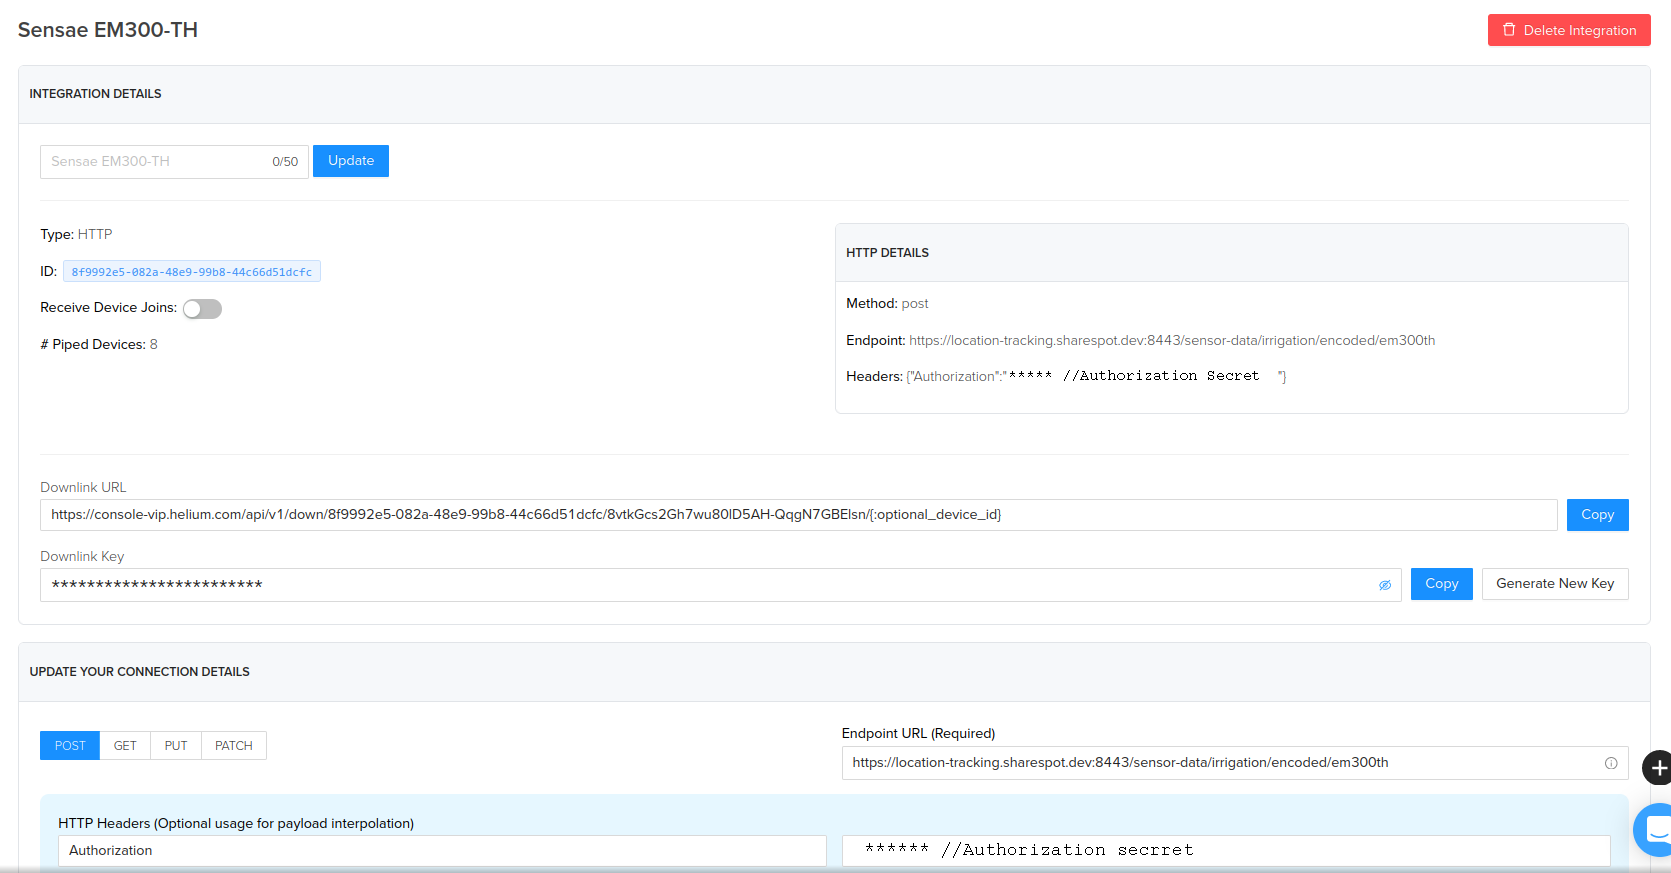
\includegraphics{assets/figures/sensor/integration.png}
    }
    \caption[Helium Custom Integration Page]{Helium Custom Integration Page}
    \label{fig:implementation:description:sensor:integration}
\end{figure}

Finally, in the \citetitle{helium} flows page, connect the registered device to the custom integration.

This method will require the user to register the endpoint with the \textit{encoded} type and write a \textbf{Data Decoder} in \textbf{Sensae Console} to translate the payload sent by the device though \citetitle{helium}.

If the user intends to use the \textbf{Data Processor}, he/she needs to:

\begin{itemize}
    \item Register the endpoint with the \textit{decoded} type;
    \item Define a \textbf{Data Processor} in \textbf{Sensae Console} to map the payload sent by \citetitle{helium};
    \item Write the decoder in \citetitle{helium} - in the \textit{Function} page;
    \item Link the device to the \textit{Function} in \citetitle{helium};
    \item Link the \textit{Function} to the custom integration;
\end{itemize}

\section{Testing}
\label{sec:implementation:testing}

According to \cite{booktest}: ``Software testing is the activity of running a series of dynamic executions of software programs after the software source code has been developed.''
Tests have a fundamental role in the development of software, they validate the the work done, prevent production bugs, regressions and improve code quality, according to \cite{linuxtest} and \cite{imbtest}.

According to \cite{typetest} there are seven categories of tests:

\begin{itemize}
    \item \textbf{Unit Testing}: Capture the need to verify and validate the individual behavior of small pieces of the solution.
    \item \textbf{Integration Testing}: Capture the need to verify that different modules/components of the system work collectively as expected;
    \item \textbf{Functional Testing}: Capture the need to verify that business requirements are meet by the system;
    \item \textbf{End-to-End Testing}: Capture the need to verify that user interaction against common workflows works as expected in the system;
    \item \textbf{Acceptance Testing}: Capture the need to ensure that functional and non-functional requirements are accomplished;
    \item \textbf{Performance Testing}: Capture the need to verify how the environment behaves under heavy load. Their objective is to evaluate the stability, availability and reliability of the system;   
    \item \textbf{Smoke Testing}: Capture the need to verify the overall state of the system before running heavier and extensive tests.
\end{itemize}

These categories complement each other to ensure the correct behavior of the system. Nevertheless, the Smoke and Acceptance Testing categories were not pursuit.

The smoke tests were replaced by common unit tests. The acceptance tests weren't required since, at the time of writing, the project had no clear and concise functional requirements that the platform could be tested against.

Architectural tests were added to the test suite to ensure that the Design discussed in the \nameref{subsubsec:design:architecture:components:logical} Section would always be respected.

The performance tests will be discussed in depth in the \nameref{chap:evaluation} Chapter.

In the following sections examples for each test category will be presented.

\subsection{Unit Tests}
\label{subsec:implementation:tests:unit}

This section focus on unit tests preformed in various containers.

The test presented in Listing~\ref{code:implementation:tests:unit1} verifies that a value referenced via the path \textit{'path[0].prop'} can be found and transferred to the path defined in the mentioned Property: \textit{DEVICE\_ID}. 
It uses the \citetitle{junit5}.

\begin{lstlisting}[style=Java, caption=Unit Test Example in \textit{iot-core} package, label={code:implementation:tests:unit1}]
$$@Test
void ensureTransferWorksWithValidArrayPath() throws JsonProcessingException {
    var jsonNode = mapper.readTree("""
            {
                "path": [
                    {
                        "prop": "viva"
                    }
                ]
            }
            """);
    var objectNode = mapper.createObjectNode();

    new KnownPropertyTransformation(
        "path[0].prop", PropertyName.DEVICE_ID, 2)
            .transfer(jsonNode, objectNode);

    Assertions.assertEquals("viva",
     objectNode.get("device").get("id").asText());
}
\end{lstlisting}

The test presented in Listing~\ref{code:implementation:tests:unit2} verifies that a user with the appropriate permissions can fetch a decoder and the last time it was used. This test relies on database access to fetch decoders and access to an RSA file to verify the authenticity of the user's access token. Since this is a unit test and its responsibility is not to verify the solution integration, it mocks the classes that access the mentioned resources using the \citetitle{mockito}.

This test only verifies the isolated behavior of the service \textit{DataDecoderCollectorService} - line \textbf{14} - other classes that the service needs are mocked and then injected in it with the annotation \textit{@InjectMocks}.

\begin{lstlisting}[style=Java, caption=Unit Test - Data Decoder Backend Container, label={code:implementation:tests:unit2}]
$$@Mock
DataDecoderCollector collector;

$$@Mock
DataDecoderMapper mapper;

$$@Mock
TokenExtractor tokenExt;

$$@Mock
LastTimeSeenDecoderRepository repository;

$$@InjectMocks
DataDecoderCollectorService service;

$$@Test
void ensureServiceWorksWhenUserHasPermissionsAndDecoderWasNeverUsed() {
    var decoder = CommonObjectsFactory.dataDecoder();

    Mockito.when(tokenExt.extract(Mockito.any(AccessTokenDTO.class)))
            .thenReturn(CommonObjectsFactory.validTenantInfo());
    Mockito.when(collector.collect()).thenReturn(Stream.of(decoder));

    var list = service.collectAll(new FakeAccessTokenDTO()).toList();

    Mockito.verify(tokenExt, Mockito.times(1))
        .extract(Mockito.any(AccessTokenDTO.class));
    Mockito.verify(collector, Mockito.times(1)).collect();
    Mockito.verify(mapper, Mockito.times(1)).domainToDto(decoder, 0L);

    Assertions.assertEquals(list.size(), 1);
}
\end{lstlisting}

The Listing~\ref{code:implementation:tests:unit3} presents some tests that verify the behavior of \textit{DeviceCommand}. This test relies in the \citetitle{jest}.

\begin{lstlisting}[style=javascript, caption=Unit Test - Device Management Frontend Model Library, label={code:implementation:tests:unit3}]
describe('Device Command Unit Test', () => {
    it('should deep clone every single parameter', () => {
        const deviceCommand = 
            new DeviceCommand('openValve', 'openValve', 'ldcn', 0, 70);
        const clone = deviceCommand.clone();
        expect(clone.id).toBe(deviceCommand.id);
        expect(clone.name).toBe(deviceCommand.name);
        expect(clone.ref).toBe(deviceCommand.ref);
        expect(clone.payload).toBe(deviceCommand.payload);
        expect(clone.port).toBe(deviceCommand.port);
    });
    it('should be invalid when it has no id', () => {
        const deviceCommand =
            new DeviceCommand('', 'openValve', 'ldcn', 0, 70);
        expect(deviceCommand.isValid()).toBeFalsy();
    });
});
\end{lstlisting}

\subsection{Integration Tests}
\label{subsec:implementation:tests:integration}

This section, as an example, starts to focus on integration tests preformed in the \textbf{Device Ownership Flow} Container and then moves on to \textbf{Notification Management Backend}.

The tool used to ease the formulation of integration tests was \citetitle{testcontainers}. This tool uses docker to fabricate the needed environment where integration tests can run.

The code in Listing~\ref{code:implementation:tests:inte1} verifies that the message broker can be reached by \textbf{Device Ownership Flow}.

\begin{lstlisting}[style=Java, caption=Integration Test - Message Broker - \textbf{Device Ownership Flow}, label={code:implementation:tests:inte1}]
$$@QuarkusTest
class DeviceInformationEmitterTest {

    $$@Inject
    DeviceInformationEmitter emitter;

    $$@Inject
    RoutingKeysProvider provider;

    $$@Inject
    $$@Any
    InMemoryConnector connector;

    $$@Test
    void testEmitterCanReachRabbitMQ() {
        var unknown = provider
            .getInternalTopicBuilder(RoutingKeysBuilderOptions.SUPPLIER)
            .withContainerType(ContainerTypeOptions.IDENTITY_MANAGEMENT)
            .withContextType(ContextTypeOptions.DEVICE_IDENTITY)
            .withOperationType(OperationTypeOptions.UNKNOWN)
            .build().orElseThrow();

        var deviceId = DeviceId.of(UUID.randomUUID());
        
        emitter.next(new DeviceTopicMessage(deviceId, unknown));

        var payload = connector.sink("egress-device-ownership")
                .received().get(0).getPayload();
        
        Assertions.assertNotNull(payload);
    }
}
\end{lstlisting}

The class tested is \textit{DeviceInformationEmitter}, line \textbf{5}, as we can see, a message is sent in line \textbf{25} and, as expected it is recieved in line \textbf{27}.

The code in Listing~\ref{code:implementation:tests:inte2} verifies that the database can be reached by the \textbf{Notification Management Backend}.

\begin{lstlisting}[style=Java, caption=Integration Test - Database - \textbf{Notification Management Backend}, label={code:implementation:tests:inte2}]
public class NotificationRepositoryImplTest extends IntegrationTest {

    $$@Autowired
    NotificationRepositoryImpl repository;

    $$@Test
    public void ensureDatabaseCanBeReached() {
        var single = Domains.single(DomainId.of(UUID.randomUUID()));
        var type = ContentType.of("a", "a", NotificationLevel.CRITICAL);
        var query = NotificationBasicQuery.of(single, List.of(type));
        
        Assertions.assertDoesNotThrow(() -> repository.find(query));
    }
}    
\end{lstlisting}

This test verifies that the \textit{NotificationRepositoryImpl} can reach the database by ensuring that no exception is thrown when executing a query to it. This class extends \textit{IntegrationTest}, the behavior of it is similar to the \textit{IntegrationTest} class discussed in the next section. 

\subsection{Functional Tests}
\label{subsec:implementation:tests:functional}

This section, as an example, starts to focus on functional tests performed in the \textbf{Data Decoder Master Backend}. Other service and configuration scope backend containers rely on similar tests.

The tool used to ease the formulation of functional tests was, once again, \citetitle{testcontainers}. Contrary to \citetitle{quarkus}, \citetitle{springboot} doesn't provide a ready to use environment according to the application needs, for that reason, the following Listings~\ref{code:implementation:tests:func1} and \ref{code:implementation:tests:func2} present the needed setup to run functional tests using \citetitle{testcontainers} and \citetitle{springboot}.

\begin{lstlisting}[style=Java, caption=Functional Test - Message Broker - \textbf{Data Decoder Master Backend} Setup, label={code:implementation:tests:func1}]
public class DatabaseContainerTest extends PostgreSQLContainer<DatabaseContainerTest> {

    private static final String IMAGE_VERSION = "data-decoder-database";
    private static DatabaseContainerTest container;

    private DatabaseContainerTest() {
        super(DockerImageName.parse(IMAGE_VERSION)
            .asCompatibleSubstituteFor("postgres:14.5"));
    }

    public static DatabaseContainerTest getInstance() {
        if (container == null) {
            container = new DatabaseContainerTest()
                .withUsername("user")
                .withPassword("sa")
                .withEnv("POSTGRESQL_USER", "user")
                .withEnv("POSTGRESQL_PASSWORD", "sa")
                .withExposedPorts(PostgreSQLContainer.POSTGRESQL_PORT);
        }
        return container;
    }

    $$@Override
    public void stop() {
        //do nothing, JVM handles shut down
    }
}    
\end{lstlisting}

The \textit{DatabaseContainerTest} follows the Singleton Pattern to ensure that all tests use the same instance. In line \textbf{8} we can see that the base image is \citetitle{postgressql}, but the image actually used is \textit{data-decoder-database}. This image is \citetitle{postgressql} with the data decoder schema and built in line \textbf{11} of the script referenced in Listing~\ref{code:implementation:decisions:actions:testscript}. The same notion is applied for the Message Broker Container. Theses two containers are the ones that \textbf{Data Decoder Master Backend} depends on.

The Listing~\ref{code:implementation:tests:func2} presents the foundation of functional and integration tests.

\begin{lstlisting}[style=Java, caption=Functional Test - Foundation - \textbf{Data Decoder Master Backend} Setup, label={code:implementation:tests:func2}]
$$@SpringBootTest
$$@Testcontainers
$$@ContextConfiguration(initializers = {IntegrationTest.Initializer.class})
$$@ActiveProfiles(profiles = "test")
public abstract class IntegrationTest {
    static class Initializer implements 
        ApplicationContextInitializer<ConfigurableApplicationContext> {
        public void initialize(ConfigurableApplicationContext context) {
            db.withDatabaseName("decoder");
            TestPropertyValues.of(
                "spring.datasource.url=" + db.getJdbcUrl(),
                "spring.datasource.username=" + db.getUsername(),
                "spring.datasource.password=" + db.getPassword(),
                "spring.rabbitmq.host=" + mb.getHost(),
                "spring.rabbitmq.port=" + mb.getAmqpPort(),
                "spring.rabbitmq.username=" + mb.getAdminUsername(),
                "spring.rabbitmq.password=" + mb.getAdminPassword()
            ).applyTo(context.getEnvironment());
        }
    }

    $$@Container
    public static PostgreSQLContainer<?> db = 
        DatabaseContainerTest.getInstance();

    $$@Container
    public static RabbitMQContainer mb =
        MessageBrokerContainerTest.getInstance();

    protected ResultSet performQuery(String sql) throws SQLException {
        DataSource ds = getDataSource(postgresSQLContainer);
        Statement statement = ds.getConnection().createStatement();
        statement.execute(sql);
        ResultSet resultSet = statement.getResultSet();

        if (resultSet != null) resultSet.next();

        return resultSet;
    }
}
\end{lstlisting}

The application environment properties are loaded in line \textbf{10} to \textbf{18} according to the containers used. The \textit{@SpringBootTest} annotation indicates that the full application has to be started, the \textit{@TestContainers} and \textit{@Container} annotations indicate that docker containers are to be used, and the \textit{@ActiveProfiles} annotation changes the profile in use so that specific beans are not loaded.

The following sample, Listing~\ref{code:implementation:tests:func3}, presents a functional test related to the database.

\begin{lstlisting}[style=Java, caption=Functional Test - Database Interaction - \textbf{Data Decoder Master Backend}, label={code:implementation:tests:func3}]
public class DataDecodersRepositoryImplTest extends IntegrationTest {

    $$@Autowired
    DataDecodersRepositoryImpl repository;
    
    $$@AfterEach
    public void cleanUp() throws SQLException {
        performQuery("TRUNCATE decoder");
    }

    $$@Test
    public void ensureSavedDecoderCanBeFound() throws SQLException {
        var query = "INSERT INTO decoder(device_type, script) "
            + "VALUES ('lgt92', 'ascma')";
        performQuery(query).close();

        var found = repository.findById(SensorTypeId.of("lgt92"))
            .orElseThrow();

        Assertions.assertEquals("lgt92", found.id().value());
        Assertions.assertEquals("ascma", found.script().value());
    }
}
\end{lstlisting}

As we can see this test extends the foundation described before. In line \textbf{4} the service to be tested, \textit{DataDecodersRepositoryImpl}, is loaded. In the test presented a new Data Decoder is stored directly in the database and then the repository service attempts to fetch it. A database clean up is preformed after each test as described in lines \textbf{6} to \textbf{9}.

The test presented in Listing~\ref{code:implementation:tests:func4}, verifies the correct interaction with the message broker container.

\begin{lstlisting}[style=Java, caption=Functional Test - Message Broker Interaction - \textbf{Data Decoder Master Backend}, label={code:implementation:tests:func4}]
public class DataDecoderInfoEmitterTest extends IntegrationTest {

    $$@Autowired
    DataDecoderHandlerService publisher;

    $$@Autowired
    RabbitAdmin rabbitAdmin;

    $$@Autowired
    RabbitTemplate amqpTemplate;

    $$@Autowired
    RoutingKeysProvider provider;

    $$@BeforeEach
    public void init() {
        if (rabbitAdmin.getQueueInfo("info") == null) {
            var supplierBuilder = RoutingKeysBuilderOptions.SUPPLIER;
            var keys = provider
                .getInternalTopicBuilder(supplierBuilder)
                .withContextType(ContextTypeOptions.DATA_DECODER)
                .withContainerType(ContainerTypeOptions.DATA_DECODER)
                .withOperationType(OperationTypeOptions.INFO)
                .build().orElseThrow();
            var queue = QueueBuilder.durable("info").build();
            rabbitAdmin.declareQueue(queue);
            rabbitAdmin.declareBinding(BindingBuilder.bind(queue)
                .to(new TopicExchange(IoTCoreTopic.INTERNAL_EXCHANGE))
                .with(keys.toString()));
        }
    }

    $$@Test
    public void ensureNewDecoderIsSentAsExpected() {
        publisher.publishUpdate(new DataDecoder(
            SensorTypeId.of("lgt92"), SensorTypeScript.of("asmc")));

        var dto = (DataDecoderNotificationDTOImpl) 
            amqpTemplate.receiveAndConvert("info");
        
        var type = DataDecoderNotificationTypeDTOImpl.UPDATE;

        Assertions.assertEquals(type, dto.type);
        Assertions.assertEquals("lgt92", dto.sensorType);
        Assertions.assertEquals("asmc", dto.information.script);
    }
}
\end{lstlisting}

In this test the class to verify is the \textit{DataDecoderHandlerService}. Once again this test extends the \textit{IntegrationTest} class. Using \textit{RabbitAdmin}, its created a queue that subscribes to the expected type of routing keys in lines \textbf{18} to \textbf{29} and then bind to the expected topic - \textit{INTERNAL\_TOPIC}.
An update is published in line \textbf{35} using the \textit{DataDecoderHandlerService} and then captured with \textit{RabbitTemplate} in line \textbf{38}.

The \textbf{Data Gateway} Container was tested against different post requests to its data retention endpoint, an example of this tests is described in Listing~\ref{code:implementation:tests:func5}.

\begin{lstlisting}[style=Java, caption=Functional Test - Rest Client Interaction - \textbf{Data Gateway}, label={code:implementation:tests:func5}]
$$@QuarkusTest
class DataControllerTest {

    $$@Test
    public void testInfoTypeDetection() {
        var errorType = "Info Type must be of value encoded or decoded";
        given().when()
            .accept(ContentType.JSON)
            .contentType(ContentType.JSON)
            .header("Authorization", "pass")
            .post("/sensor-data/fleet/wrong/lgt92")
            .then()
            .statusCode(400)
            .body("error", containsString(errorType));
    }
}
\end{lstlisting}

This test simply attempts to send an HTTP POST request to an invalid resource - line \textbf{11}.

\subsection{End-to-End Tests}
\label{subsec:implementation:tests:endtoend}

This section presents some of the end-to-end tests of \textbf{Sensae Console}.
This tests evaluate how the system responds to various user actions.

All end-to-end tests rely on \citetitle{cypress}, an end-to-end testing framework.
To improve tests readability new cypress commands were created.
The methods \textit{anonymous}, \textit{logout} and \textit{goToIdentityPage} are some examples of this commands - Listing~\ref{code:implementation:tests:e2e2}.

\begin{lstlisting}[style=javascript, caption=End-to-End Test - Custom Commands - \textbf{UI Aggregator}, label={code:implementation:tests:e2e2}]
declare namespace Cypress {
    interface Chainable<Subject> {
        anonymous(): void;
        logout(): void;
        goToIdentityPage(): void;
    }
}
    
Cypress.Commands.add('anonymous', () => {
    console.log('Custom command: Anonymous Login');
    cy.contains('Login').click();
    cy.contains('Anonymous').click();
});
    
Cypress.Commands.add('logout', () => {
    console.log('Custom command: Logout');
    cy.get('#account').click();
    cy.contains('Logout').click();
});
    
Cypress.Commands.add('goToIdentityPage', () => {
    console.log('Custom command: go to Identity Page');
    cy.get('#tools').click();
    cy.contains('Identity Management').click();
});
\end{lstlisting}

As an example, the \textit{anonymous} command searches for something with the text \textit{Login}, and clicks on it.

The Listing~\ref{code:implementation:tests:e2e1} presents a test that ensures anyone can enter the system as an anonymous user.

\begin{lstlisting}[style=javascript, caption=End-to-End Test - Anonymous Authentication - \textbf{UI Aggregator}, label={code:implementation:tests:e2e1}]
describe('ui-aggregator', () => {
    beforeEach(() => cy.visit('/'));
    it('should display welcome message for anonymous user', () => {
        cy.anonymous();
        cy.contains("Valid Credentials");
        cy.logout();
    });
});
\end{lstlisting}

The test verifies that a successful login notification is received in line \textbf{5}. Both of the commands previously described are used in this test.

The Listing~\ref{code:implementation:tests:e2e3} presents a test that walks though the \textbf{Identity Management Page} verifying that an authenticated manager can see every available domain.

\begin{lstlisting}[style=javascript, caption=End-to-End Test - Discover Available Domains - \textbf{Identity Management}, label={code:implementation:tests:e2e3}]
describe('ui-aggregator', () => {
    beforeEach(() => cy.visit('/'));
    it('should present various default domains', () => {
        cy.managerLogin();
        cy.goToIdentityPage();
        cy.contains("root");
        cy.get(".toggle").click();
        cy.contains("public");
        cy.contains("unallocated");
    });
});
\end{lstlisting}

This test verifies that a user in the root domain can see all default domains in the \textbf{Identity Management Page}, as described in \nameref{subsubsec:design:domain:bounded_contexts:identity} Bounded Context Section.

\subsection{Architectural Tests}
\label{subsec:implementation:tests:arch}

This section presents some of the architectural tests of \textbf{Sensae Console}'s Containers. This tests are only performed in the backend containers.
As an example it will be displayed one test for the \textbf{Configuration / Service Scope} and another for the \textbf{Data Flow Scope}.

The tool used was ArchUnit, according to \cite{archunit}, it ``provides a variety of predefined governance rules codified as unit tests and allows architects to write specific tests that address modularity"".

The Listing~\ref{code:implementation:tests:arch1} presents an example of the tests made for \textbf{Configuration / Service Scope} backend containers.

\begin{lstlisting}[style=Java, caption=Architectural Test - Onion Architecture - \textbf{Device Management Master Backend}, label={code:implementation:tests:arch1}]
$$@AnalyzeClasses(packages = "pt.sensae.services")
public class ApplicationArchitectureTest {

    $$@ArchTest
    static final ArchRule architecture = Architectures
        .onionArchitecture()
        .domainModels("..domain..")
        .domainServices("..domainservices..")
        .applicationServices("..application..")
        .adapter("amqp connector", "..amqp..")
        .adapter("in memory persistence", "..memory..")
        .adapter("postgres persistence", "..postgres..")
        .adapter("graphql endpoint", "..graphql..")
        .ignoreDependency(resideInAPackage("..boot.."), alwaysTrue());

    $$@ArchTest
    static final ArchRule domainMustNotDependOnFrameworks = 
        ArchRuleDefinition.noClasses().that()
            .resideInAnyPackage("..domain..")
            .should()
            .dependOnClassesThat()
            .haveNameMatching("org.springframework.")
            .orShould()
            .dependOnClassesThat()
            .haveNameMatching("javax.persistence.")
            .because("Domain should be free from dependencies");
}
\end{lstlisting}

The test \textit{architecture} at lines \textbf{4} to \textbf{14} ensures that the onion architecture is followed. The test \textit{domainMustNotDependOnFrameworks} at lines \textbf{16} to \textbf{26} ensures that the domain and domain services components are free of dependencies.

The Listing~\ref{code:implementation:tests:arch2} presents an example of the tests made for \textbf{Data Flow Scope}.

\begin{lstlisting}[style=Java, caption=Architectural Test - Simplified Onion Architecture - \textbf{Data Processor Flow}, label={code:implementation:tests:arch2}]
$$@AnalyzeClasses(packages = "pt.sensae.services")
public class ArchitecturalTest {

    $$@ArchTest
    static final ArchRule architecture = Architectures
        .onionArchitecture()
        .domainModels("..domain..")
        .applicationServices("..application..")
        .adapter("amqp internal topic connector", "..internal..")
        .adapter("amqp ingress data topic connector", "..ingress..")
        .adapter("amqp egress data topic connector", "..egress..")
        .adapter("in memory persistence", "..memory..")
        .ignoreDependency(resideInAPackage("..boot.."), alwaysTrue())
        .allowEmptyShould(true);

    $$@ArchTest
    static final ArchRule domainMustNotDependOnFrameworks = 
        ArchRuleDefinition.noClasses().that()
            .resideInAnyPackage("..domain..")
            .should().dependOnClassesThat()
            .haveNameMatching("org.eclipse.")
            .orShould().dependOnClassesThat()
            .haveNameMatching("com.fasterxml.")
            .orShould().dependOnClassesThat()
            .haveNameMatching("com.google.")
            .orShould().dependOnClassesThat()
            .haveNameMatching("javax.")
            .because("Domain should be free from Frameworks");
}
\end{lstlisting}

The test \textit{architecture} at lines \textbf{4} to \textbf{12} ensures that, such as the previous test, the onion architecture is followed. The difference between the two is that this one allows empty components - line \textbf{12}, since the \textbf{Data Flow Scope} containers have no domain services. The test \textit{domainMustNotDependOnFrameworks} at lines \textbf{14} to \textbf{26} ensures that the domain component are free of dependencies.

\section{Synopsis}
\label{sec:implementation:synopsis}

This chapter introduced the most important technical decisions taken during the solution's implementation. This decisions were followed with a technical description of \textbf{Sensae Console} tailored for those who manage and develop the platform.
Lastly some of the tests that ensure the proper operation of the solution were presented.

In the next chapter, \nameref{chap:evaluation}, the performance of the platform will be extensively discussed.

\chapter{Evaluation}
\label{chap:evaluation}

This chapter intent is to describe the evaluations preformed against the solution. For that the following sections will tackle:

\begin{itemize}
    \item Objectives and execution environment of this evaluation;
    \item Approach applied to evaluate the software developed;
    \item Drafted experiences and results collected;
    \item Analysis of the results collected;
    \item Observations taken from the analysis conducted.
\end{itemize}

The expected behavior of the system according to functional requirements can be attested with deterministic tests presented in Section~\ref{sec:implementation:testing}. On the other hand, some non-functional requirements, such as performance and usability requirements, can't be deterministically attested with simple tests.

Since the company and this project's solution were both in the early stages of conception no strick usability requirements were defined. The experiences here documented focus on the performance of the solution according to the points defined in Section~\ref{sec:requirements:non_functional}.

\section{Objectives}
\label{sec:evaluation:objectives}

The objective of this evaluation is to determine the throughput limits of the entire solution (\textbf{Sensae Console} and \textbf{External Services}) regarding data ingestion, within the requirements detailed in Section~\ref{sec:requirements:non_functional}.

Since the solution was designed to scale infinitely and handle high-levels of throughput, the performance of it in a multi-organization and shared infrastructure is undermined. The evaluation should instead focus on environments where resources are constrained.

Therefore, the performance of the solution will be tested against above-average usage conditions of small to medium organizations that require a dedicated infrastructure, either on-site or in the cloud.

This type of organizations encompass entities such as:

\begin{itemize}
    \item Public Institutes: town councils, public transportation organizations, waste management departments and others;
    \item Private owned business: chicken farms, greenhouse farms, goods transportation agencies, industrial warehouses, agriculture cooperatives and others;
\end{itemize}

The objective is to determine the platform limits of data ingestion, processing, storage and real-time supply within the desired requirements.

This evaluation also helps to understand what components are the first to degrade the performance of the system.

\section{Approach}
\label{sec:evaluation:approach}

The approach taken to evaluate the solution was to send increasingly higher volumes of HTTP requests to the \nameref{subsec:implementation:description:ingestion} in order to determine the platform limits of healthy operation.

Given the type of organizations that require this deployment mode it is expected that the number of devices installed doesn't go beyond 500\footnote{500 devices in use by a single entity is expected to be a huge amount of devices for the realistic business needs of small/medium organizations}.

The evaluation encompasses 3 test scenarios, one for each developed service: (i) Fleet Management, (i) Smart Irrigation, (iii) Notification Management.

The performance tests use the \citetitle{k6} tool. This tool allows one to design performance tests entirely in \textit{Javascript}. An example of the scripts developed is presented in Appendix~\ref{AppendixF}. The \citetitle{k6} tool produces various metrics that are then analyzed using \textit{R}, an example of the analysis scripts developed is presented in Appendix~\ref{AppendixG}.

For simplicity, the solution was deployed in a \gls{VM} Instance of the Google Cloud Platform, type \textit{'e2-standard-4'}, with the following specs:

\begin{itemize}
    \item Memory: 16 GB;
    \item Number of vCPU Cores: 4;
    \item Disk Type: Balanced Persistence Disk.
\end{itemize}

As of September, 2022, the cost associated with this \gls{VM} rounds the 100\texteuro per month.

This tests were executed through the author' machine which may undermine the communication with the \gls{VM} Instance, e.g. number of HTTP requests and stability of the Websocket connection.

The approach taken isn't an attempt to mimic normal usage patterns but simply to envision the platform throughput limits. Even though an approach closer to the reality would present results easier to interpreter, it would take to much time to design, implement and run this realistic tests. Therefore, metrics such as the interval between two consecutive Uplinks of the same device, were severely narrowed.

\section{Experiences}
\label{sec:evaluation:experiences}

As described before, 3 scenarios that emulate a variable number of devices sending uplinks to \textbf{Sensae Console} were tested:

\begin{itemize}
    \item \textbf{Scenario 1}: Fleet Management;
    \item \textbf{Scenario 2}: Smart Irrigation;
    \item \textbf{Scenario 3}: Notification Management;
\end{itemize}

Each scenario examines the time it takes to notify a user about a measure or notification since the system collected the correspondent data unit.

The tests preformed against the system ensured that no Device Information, Device Ownership, Data Decoders or Data Processors were cached in the \textbf{Data Flow} Scope to create even harsher conditions.

In order to focus on the raw performance of the system, the following conjectures were applied:

\begin{itemize}
    \item A single type of Data Decoder is used to decode Data Units;
    \item A single type of Data Processor is used to process Data Units;
    \item The Data Units sent will evenly require a Data Decoder or a Data Processor;
    \item The Data Decoder and Data Processor operations are identical, meaning that, given the same input, both must provide the same output;
    \item A single \textit{Anonymous user} is notified about new measures or notifications;
    \item Each scenario focus on a single business case in the \textbf{Service} Scope;
    \item All devices belong to the \textit{Public} Domain (this eases the process of authentication);
    \item No erroneous data will is sent, e.g. data units with unknown data decoders/processors/devices, incorrect measures or invalid structure;
    \item The default configuration regarding database connection pools, cache size, cache eviction policies and others is used;
    \item Ten iterations of requests are sent in each experience, each iteration sends one Data Unit per Device;
\end{itemize}

The Table~\ref{tab:evaluation:experiences:summary} summarizes the experiences preformed.

\begin{table}[H]
    \caption{Details about the experiences performed}
    \label{tab:evaluation:experiences:summary}
    \centering
    \begin{tabular}{@{}ccccc@{}}
    \toprule
    \textbf{Experience} &
      \textbf{\begin{tabular}[c]{@{}l@{}}Number of\\ Devices\end{tabular}} &
      \textbf{\begin{tabular}[c]{@{}l@{}}Interval between\\ device uplinks\end{tabular}} &
      \textbf{\begin{tabular}[c]{@{}l@{}}Average number of\\ uplinks per second\end{tabular}} & \textbf{\begin{tabular}[c]{@{}l@{}}Total number \\of Uplinks\end{tabular}} \\ \midrule
    A & 100  & 10 seconds & 9  & 1000 \\ \midrule
    B & 200  & 10 seconds & 18  & 2000 \\ \midrule
    C & 500  & 10 seconds & 45  & 5000 \\ \midrule
    D & 1000 & 10 seconds & 90 & 10000 \\ \midrule
    E & 100  & 3 seconds  & 25  & 1000 \\ \midrule
    F & 200  & 3 seconds  & 50  & 2000 \\ \midrule
    G & 500  & 3 seconds  & 125 & 5000 \\ \midrule
    H & 1000 & 3 seconds  & 250 & 10000 \\ \bottomrule
    \end{tabular}
\end{table}

The results of each scenario will be presented in the next sections. The results will be displayed in a table with the following metrics: (i) average, (ii) minimum, (iii) median, (iv) maximum, (v) 90th Percentile and (vi) 95 Percentile.

\subsection{Fleet Management Experience Scenario}
\label{subsec:evaluation:experiences:fleet}

This scenario focus on the Fleet Management Service. The Table~\ref{tab:evaluation:experiences:fleet:results} presents the results related to the time is takes for a Data Unit to be processed and supplied as a measure to the user.

\begin{table}[H]
    \caption{Results for the Fleet Management Scenario (in seconds)}
    \label{tab:evaluation:experiences:fleet:results}
    \centering
    \begin{tabular}{@{}ccccccc@{}}
    \toprule
    \textbf{Experience} & \textbf{Average} & \textbf{Min} & \textbf{Median} & \textbf{Max} & \textbf{90\% Percentile} & \textbf{95\% Percentile} \\ \midrule
    A & 0.206 & 0.182 & 0.193 & 0.765 & 0.205 & 0.215 \\ \midrule
    B & 0.207 & 0.182 & 0.193 & 0.770 & 0.211 & 0.220 \\ \midrule
    C & 0.225 & 0.184 & 0.209 & 0.921 & 0.241 & 0.257 \\ \midrule
    D & 2.871 & 0.189 & 0.674 & 16.69 & 10.14 & 13.31 \\ \midrule
    E & 0.213 & 0.185 & 0.200 & 0.780 & 0.214 & 0.220 \\ \midrule
    F & 0.214 & 0.180 & 0.200 & 0.789 & 0.224 & 0.235 \\ \midrule
    G & 0.921 & 0.183 & 0.754 & 2.992 & 2.015 & 2.326 \\ \midrule
    H & 38.43 & 0.218 & 35.39 & 83.37 & 71.52 & 77.08 \\ \bottomrule
    \end{tabular}
\end{table}

This results show that, a system focused on the Fleet Management business case, can successfully handle 125 Data Units per second while answering the defined requirements.

The experience \textbf{H} had the measures supplied with a delay of 40 seconds on average, this results are far from the optimal response time defined in the requirements.

Currently, the devices used in production for this business case send, at best, measures every minute, this means that the real number of devices is much higher than the one determined by this tests.

\subsection{Smart Irrigation Experience Scenario}
\label{subsec:evaluation:experiences:irrigation}

This scenario focus on the Smart Irrigation Service. The Table~\ref{tab:evaluation:experiences:irrigation:results} presents the results related to the time is takes for a Data Unit to be processed, stored and supplied as a measure to the user.

\begin{table}[H]
    \caption{Results for the Smart Irrigation Scenario (in seconds)}
    \label{tab:evaluation:experiences:irrigation:results}
    \centering
    \begin{tabular}{@{}ccccccc@{}}
    \toprule
    \textbf{Experience} & \textbf{Average} & \textbf{Min} & \textbf{Median} & \textbf{Max} & \textbf{90\% Percentile} & \textbf{95\% Percentile} \\ \midrule
    A & 0.204 & 0.181 & 0.190 & 0.761 & 0.202 & 0.210 \\ \midrule
    B & 0.211 & 0.182 & 0.199 & 0.772 & 0.220 & 0.233 \\ \midrule
    C & 0.389 & 0.183 & 0.299 & 1.290 & 0.760 & 0.978 \\ \midrule
    D & 20.72 & 0.205 & 21.85 & 44.16 & 36.98 & 41.02 \\ \midrule
    E & 0.221 & 0.182 & 0.205 & 0.767 & 0.242 & 0.254 \\ \midrule
    F & 4.358 & 0.187 & 2.925 & 15.69 & 10.46 & 13.10 \\ \midrule
    G & 12.95 & 0.255 & 13.71 & 20.00 & 14.60 & 15.34 \\ \midrule
    H & 70.06 & 0.260 & 70.98 & 122.3 & 109.8 & 115.4 \\ \bottomrule
    \end{tabular}
\end{table}

This results show that, a system focused on the Smart Irrigation business case, can successfully handle 45 Data Units per second while answering the defined requirements. The experiences \textbf{D}, \textbf{F}, \textbf{G}, \textbf{H} shed a light on the possible limits for this Service.

The results captured in this experiences infer that this system can comfortably withstand a throughput of around 500 devices, each sending their measures every 10 seconds without undermining its overall behavior.

Currently, the devices used in production for this business case send measures every 10 minutes, this means that the real number of devices is much higher than the one determine by this tests.

\subsection{Notification Management Experience Scenario}
\label{subsec:evaluation:experiences:notification}

This scenario focus on the Notification Management Service. The Table~\ref{tab:evaluation:experiences:notification:results} presents the results related to the time is takes for a Data Unit to be processed and trigger a new alert that is  supplied to the user as a notification.

In this experience it was simulated that an average of 10\% of the data units would produce an alert.

\begin{table}[H]
    \caption{Results for the Notification Management Scenario (in seconds)}
    \label{tab:evaluation:experiences:notification:results}
    \centering
    \begin{tabular}{@{}ccccccc@{}}
    \toprule
    \textbf{Experience} & \textbf{Average} & \textbf{Min} & \textbf{Median} & \textbf{Max} & \textbf{90\% Percentile} & \textbf{95\% Percentile} \\ \midrule
    A & 0.268 & 0.208 & 0.226 & 1.697 & 0.265 & 0.308 \\ \midrule
    B & 0.263 & 0.196 & 0.223 & 1.735 & 0.245 & 0.266 \\ \midrule
    C & 0.434 & 0.199 & 0.235 & 4.029 & 0.287 & 2.364 \\ \midrule
    D & 1.678 & 0.195 & 0.241 & 11.95 & 6.885 & 9.728 \\ \midrule
    E & 0.334 & 0.207 & 0.230 & 3.947 & 0.323 & 0.372 \\ \midrule
    F & 0.856 & 0.200 & 0.241 & 5.629 & 2.379 & 4.875 \\ \midrule
    G & 10.02 & 1.188 & 11.09 & 19.08 & 14.01 & 15.03 \\ \midrule
    H & 27.51 & 13.48 & 27.77 & 35.50 & 29.68 & 31.14 \\ \bottomrule
    \end{tabular}
\end{table}

The results captured in this experiences infer that this system can comfortably withstand a throughput of around 500 devices (each sending measures every 10 seconds) without undermining its overall behavior.

\section{Discussion of the overall results}
\label{subsubsec:evaluation:overview}

As seen by the experiences preformed the system was capable of answering the defined requirements.

Apart from the results gathered it is important to mention the following findings:

\begin{itemize}
    \item The system answered all HTTP requests within an average of 0.2 seconds;
    \item There was no visible performance discrepancy between the use of Data Decoders versus Data Processors;
    \item The bootstrapping of \textbf{Data Flow} Caches is noticeable in most experiences, specially the lighter ones. The first iteration usually takes the longer to be processed when the system is not overwhelmed;
    \item The system was always capable of storing all the measures and alerts;
\end{itemize}

The experiences performed helped to determine the platform throughput limits but didn't indicated what components were underperforming and degrading the results.

In the following sections some components are individually evaluated so that the bottlenecks of the system can be found.

Looking at the architecture the five logical bottlenecks are:

\begin{itemize}
    \item The \nameref{subsec:implementation:description:ingestion} that collects requests (in the \textbf{Data Relayer} Container);
    \item The databases in the \textbf{External Services Scope} that store measures or notifications;
    \item The \textbf{Message Broker} that routes data units through the system;
    \item The Websocket implementation used by GraphQL to supply measures and notifications in the Backends of the \textbf{External Services Scope};
    \item The process of filling the \textbf{Data Flow Scope} Caches with the information managed by the various containers in the \textbf{Configuration Scope}.
\end{itemize}

\subsection{Data Ingestion Endpoint Performance}
\label{subsec:evaluation:overview:endpoint}

In order to evaluate this piece of the system first the \textbf{H} experiences of each scenario are presented since they represent the higher throughput of all experiences preformed.

This experiences yielded the following results:

\begin{table}[H]
    \caption{Data Ingestion Endpoint response time results (in milliseconds)}
    \label{tab:evaluation:overview:endpoint:results}
    \centering
    \begin{tabular}{@{}ccccccc@{}}
    \toprule
    \textbf{Scenario} & \textbf{Average} & \textbf{Min} & \textbf{Median} & \textbf{Max} & \textbf{90\% Percentile} & \textbf{95\% Percentile} \\ \midrule
    1 & 193.24 & 170.02 & 182.12 & 581.6 & 219.16 & 249.24 \\ \midrule
    2 & 227.48 & 169.19 & 200.17 & 727.11 & 319.77 & 376.98 \\ \midrule
    3 & 179.83 & 167.09 & 178.99 & 2632 & 186.36 & 189.27 \\ \bottomrule
    \end{tabular}
\end{table}

This results present a stable performance even under a high number of requests, apart from the maximum value obtained in scenario 2, a clear outlier, all requests were answered within a second.

In order to find the amount of requests that would leave the system unresponsive more tests were performed, this tests only focused on the Data Ingestion Endpoint responses. The system was capable of ingesting around 600 requests per second before starting to dropping requests.

\subsection{Data Processor versus Data Decoder Performance}
\label{subsec:evaluation:overview:decoproc}

The experiences preformed also helped to understand if the Data Decoder  underperformed when compared to the Data Processor. This was the expected result since the Data Decoder uses an embedded \textit{Javascript} engine to process data units, and the Data Processor relies only on \textit{Java} to process messages.

As an example, the following chart presented in Figure~\ref{fig:evaluation:overview:decoproc:chart:s3eC} helps to debunk this belief.

\begin{figure}[H]
    \centering
    % Created by tikzDevice version 0.12.3.1 on 2022-09-25 17:35:01
% !TEX encoding = UTF-8 Unicode
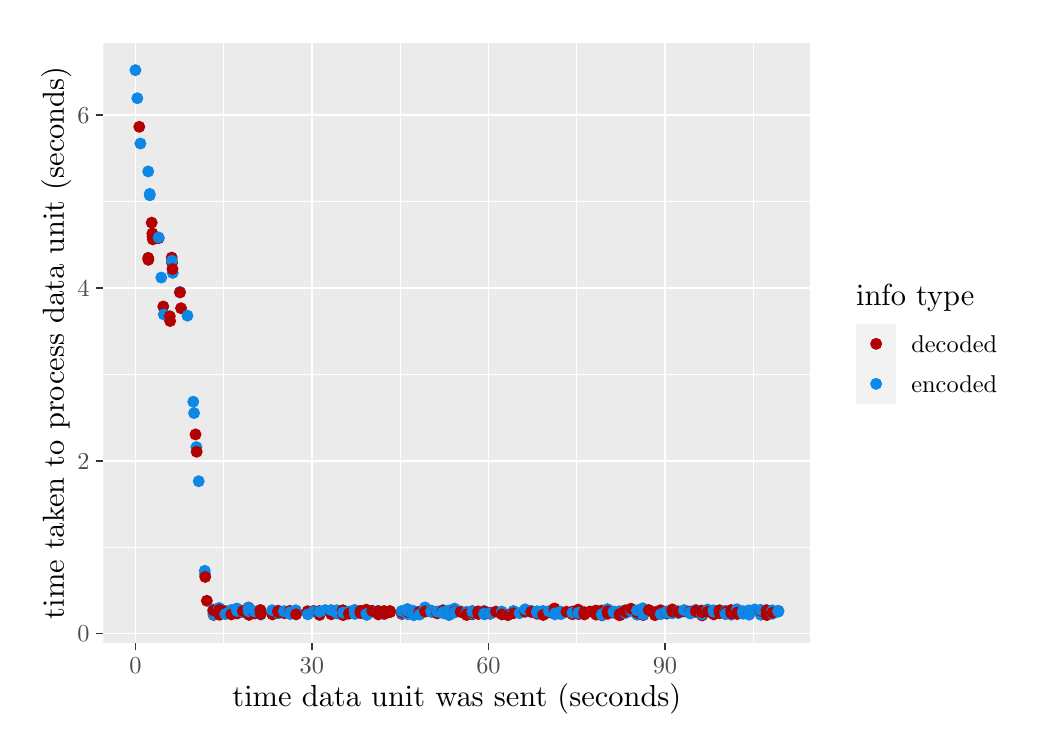
\begin{tikzpicture}[x=1pt,y=1pt]
\definecolor{fillColor}{RGB}{255,255,255}
\path[use as bounding box,fill=fillColor,fill opacity=0.00] (0,0) rectangle (361.35,252.94);
\begin{scope}
\path[clip] (  0.00,  0.00) rectangle (361.35,252.94);
\definecolor{drawColor}{RGB}{255,255,255}
\definecolor{fillColor}{RGB}{255,255,255}

\path[draw=drawColor,line width= 0.6pt,line join=round,line cap=round,fill=fillColor] (  0.00,  0.00) rectangle (361.35,252.94);
\end{scope}
\begin{scope}
\path[clip] ( 27.31, 30.69) rectangle (282.86,247.45);
\definecolor{fillColor}{gray}{0.92}

\path[fill=fillColor] ( 27.31, 30.69) rectangle (282.86,247.45);
\definecolor{drawColor}{RGB}{255,255,255}

\path[draw=drawColor,line width= 0.3pt,line join=round] ( 27.31, 65.24) --
	(282.86, 65.24);

\path[draw=drawColor,line width= 0.3pt,line join=round] ( 27.31,127.70) --
	(282.86,127.70);

\path[draw=drawColor,line width= 0.3pt,line join=round] ( 27.31,190.16) --
	(282.86,190.16);

\path[draw=drawColor,line width= 0.3pt,line join=round] ( 70.82, 30.69) --
	( 70.82,247.45);

\path[draw=drawColor,line width= 0.3pt,line join=round] (134.61, 30.69) --
	(134.61,247.45);

\path[draw=drawColor,line width= 0.3pt,line join=round] (198.39, 30.69) --
	(198.39,247.45);

\path[draw=drawColor,line width= 0.3pt,line join=round] (262.17, 30.69) --
	(262.17,247.45);

\path[draw=drawColor,line width= 0.6pt,line join=round] ( 27.31, 34.01) --
	(282.86, 34.01);

\path[draw=drawColor,line width= 0.6pt,line join=round] ( 27.31, 96.47) --
	(282.86, 96.47);

\path[draw=drawColor,line width= 0.6pt,line join=round] ( 27.31,158.93) --
	(282.86,158.93);

\path[draw=drawColor,line width= 0.6pt,line join=round] ( 27.31,221.38) --
	(282.86,221.38);

\path[draw=drawColor,line width= 0.6pt,line join=round] ( 38.93, 30.69) --
	( 38.93,247.45);

\path[draw=drawColor,line width= 0.6pt,line join=round] (102.71, 30.69) --
	(102.71,247.45);

\path[draw=drawColor,line width= 0.6pt,line join=round] (166.50, 30.69) --
	(166.50,247.45);

\path[draw=drawColor,line width= 0.6pt,line join=round] (230.28, 30.69) --
	(230.28,247.45);
\definecolor{drawColor}{RGB}{179,0,0}
\definecolor{fillColor}{RGB}{179,0,0}

\path[draw=drawColor,line width= 0.4pt,line join=round,line cap=round,fill=fillColor] ( 40.32,217.11) circle (  1.96);

\path[draw=drawColor,line width= 0.4pt,line join=round,line cap=round,fill=fillColor] ( 43.55,169.76) circle (  1.96);

\path[draw=drawColor,line width= 0.4pt,line join=round,line cap=round,fill=fillColor] ( 43.60,169.05) circle (  1.96);
\definecolor{drawColor}{RGB}{13,136,230}
\definecolor{fillColor}{RGB}{13,136,230}

\path[draw=drawColor,line width= 0.4pt,line join=round,line cap=round,fill=fillColor] ( 38.93,237.59) circle (  1.96);

\path[draw=drawColor,line width= 0.4pt,line join=round,line cap=round,fill=fillColor] ( 40.73,211.08) circle (  1.96);

\path[draw=drawColor,line width= 0.4pt,line join=round,line cap=round,fill=fillColor] ( 39.62,227.44) circle (  1.96);

\path[draw=drawColor,line width= 0.4pt,line join=round,line cap=round,fill=fillColor] ( 44.13,192.37) circle (  1.96);
\definecolor{drawColor}{RGB}{179,0,0}
\definecolor{fillColor}{RGB}{179,0,0}

\path[draw=drawColor,line width= 0.4pt,line join=round,line cap=round,fill=fillColor] ( 45.15,177.45) circle (  1.96);

\path[draw=drawColor,line width= 0.4pt,line join=round,line cap=round,fill=fillColor] ( 45.07,178.57) circle (  1.96);
\definecolor{drawColor}{RGB}{13,136,230}
\definecolor{fillColor}{RGB}{13,136,230}

\path[draw=drawColor,line width= 0.4pt,line join=round,line cap=round,fill=fillColor] ( 44.10,192.87) circle (  1.96);
\definecolor{drawColor}{RGB}{179,0,0}
\definecolor{fillColor}{RGB}{179,0,0}

\path[draw=drawColor,line width= 0.4pt,line join=round,line cap=round,fill=fillColor] ( 44.81,182.47) circle (  1.96);
\definecolor{drawColor}{RGB}{13,136,230}
\definecolor{fillColor}{RGB}{13,136,230}

\path[draw=drawColor,line width= 0.4pt,line join=round,line cap=round,fill=fillColor] ( 43.55,200.99) circle (  1.96);
\definecolor{drawColor}{RGB}{179,0,0}
\definecolor{fillColor}{RGB}{179,0,0}

\path[draw=drawColor,line width= 0.4pt,line join=round,line cap=round,fill=fillColor] ( 45.22,176.45) circle (  1.96);

\path[draw=drawColor,line width= 0.4pt,line join=round,line cap=round,fill=fillColor] ( 47.32,176.85) circle (  1.96);
\definecolor{drawColor}{RGB}{13,136,230}
\definecolor{fillColor}{RGB}{13,136,230}

\path[draw=drawColor,line width= 0.4pt,line join=round,line cap=round,fill=fillColor] ( 47.30,177.13) circle (  1.96);

\path[draw=drawColor,line width= 0.4pt,line join=round,line cap=round,fill=fillColor] ( 48.28,162.64) circle (  1.96);
\definecolor{drawColor}{RGB}{179,0,0}
\definecolor{fillColor}{RGB}{179,0,0}

\path[draw=drawColor,line width= 0.4pt,line join=round,line cap=round,fill=fillColor] ( 49.00,152.18) circle (  1.96);
\definecolor{drawColor}{RGB}{13,136,230}
\definecolor{fillColor}{RGB}{13,136,230}

\path[draw=drawColor,line width= 0.4pt,line join=round,line cap=round,fill=fillColor] ( 49.19,149.31) circle (  1.96);
\definecolor{drawColor}{RGB}{179,0,0}
\definecolor{fillColor}{RGB}{179,0,0}

\path[draw=drawColor,line width= 0.4pt,line join=round,line cap=round,fill=fillColor] ( 51.48,146.94) circle (  1.96);

\path[draw=drawColor,line width= 0.4pt,line join=round,line cap=round,fill=fillColor] ( 51.36,148.65) circle (  1.96);
\definecolor{drawColor}{RGB}{13,136,230}
\definecolor{fillColor}{RGB}{13,136,230}

\path[draw=drawColor,line width= 0.4pt,line join=round,line cap=round,fill=fillColor] ( 52.42,164.33) circle (  1.96);
\definecolor{drawColor}{RGB}{179,0,0}
\definecolor{fillColor}{RGB}{179,0,0}

\path[draw=drawColor,line width= 0.4pt,line join=round,line cap=round,fill=fillColor] ( 52.17,167.95) circle (  1.96);

\path[draw=drawColor,line width= 0.4pt,line join=round,line cap=round,fill=fillColor] ( 52.05,169.86) circle (  1.96);
\definecolor{drawColor}{RGB}{13,136,230}
\definecolor{fillColor}{RGB}{13,136,230}

\path[draw=drawColor,line width= 0.4pt,line join=round,line cap=round,fill=fillColor] ( 52.12,168.73) circle (  1.96);
\definecolor{drawColor}{RGB}{179,0,0}
\definecolor{fillColor}{RGB}{179,0,0}

\path[draw=drawColor,line width= 0.4pt,line join=round,line cap=round,fill=fillColor] ( 52.33,165.70) circle (  1.96);
\definecolor{drawColor}{RGB}{13,136,230}
\definecolor{fillColor}{RGB}{13,136,230}

\path[draw=drawColor,line width= 0.4pt,line join=round,line cap=round,fill=fillColor] ( 55.02,157.43) circle (  1.96);
\definecolor{drawColor}{RGB}{179,0,0}
\definecolor{fillColor}{RGB}{179,0,0}

\path[draw=drawColor,line width= 0.4pt,line join=round,line cap=round,fill=fillColor] ( 55.03,157.27) circle (  1.96);

\path[draw=drawColor,line width= 0.4pt,line join=round,line cap=round,fill=fillColor] ( 55.42,151.56) circle (  1.96);
\definecolor{drawColor}{RGB}{13,136,230}
\definecolor{fillColor}{RGB}{13,136,230}

\path[draw=drawColor,line width= 0.4pt,line join=round,line cap=round,fill=fillColor] ( 57.73,148.87) circle (  1.96);

\path[draw=drawColor,line width= 0.4pt,line join=round,line cap=round,fill=fillColor] ( 59.84,117.77) circle (  1.96);

\path[draw=drawColor,line width= 0.4pt,line join=round,line cap=round,fill=fillColor] ( 60.12,113.68) circle (  1.96);
\definecolor{drawColor}{RGB}{179,0,0}
\definecolor{fillColor}{RGB}{179,0,0}

\path[draw=drawColor,line width= 0.4pt,line join=round,line cap=round,fill=fillColor] ( 60.65,105.96) circle (  1.96);
\definecolor{drawColor}{RGB}{13,136,230}
\definecolor{fillColor}{RGB}{13,136,230}

\path[draw=drawColor,line width= 0.4pt,line join=round,line cap=round,fill=fillColor] ( 64.09, 55.37) circle (  1.96);

\path[draw=drawColor,line width= 0.4pt,line join=round,line cap=round,fill=fillColor] ( 60.96,101.37) circle (  1.96);
\definecolor{drawColor}{RGB}{179,0,0}
\definecolor{fillColor}{RGB}{179,0,0}

\path[draw=drawColor,line width= 0.4pt,line join=round,line cap=round,fill=fillColor] ( 61.07, 99.69) circle (  1.96);
\definecolor{drawColor}{RGB}{13,136,230}
\definecolor{fillColor}{RGB}{13,136,230}

\path[draw=drawColor,line width= 0.4pt,line join=round,line cap=round,fill=fillColor] ( 61.80, 89.04) circle (  1.96);

\path[draw=drawColor,line width= 0.4pt,line join=round,line cap=round,fill=fillColor] ( 64.00, 56.68) circle (  1.96);
\definecolor{drawColor}{RGB}{179,0,0}
\definecolor{fillColor}{RGB}{179,0,0}

\path[draw=drawColor,line width= 0.4pt,line join=round,line cap=round,fill=fillColor] ( 64.15, 54.47) circle (  1.96);

\path[draw=drawColor,line width= 0.4pt,line join=round,line cap=round,fill=fillColor] ( 64.74, 45.85) circle (  1.96);
\definecolor{drawColor}{RGB}{13,136,230}
\definecolor{fillColor}{RGB}{13,136,230}

\path[draw=drawColor,line width= 0.4pt,line join=round,line cap=round,fill=fillColor] ( 67.08, 42.69) circle (  1.96);

\path[draw=drawColor,line width= 0.4pt,line join=round,line cap=round,fill=fillColor] ( 67.19, 41.16) circle (  1.96);

\path[draw=drawColor,line width= 0.4pt,line join=round,line cap=round,fill=fillColor] ( 67.12, 42.13) circle (  1.96);

\path[draw=drawColor,line width= 0.4pt,line join=round,line cap=round,fill=fillColor] ( 67.16, 41.57) circle (  1.96);
\definecolor{drawColor}{RGB}{179,0,0}
\definecolor{fillColor}{RGB}{179,0,0}

\path[draw=drawColor,line width= 0.4pt,line join=round,line cap=round,fill=fillColor] ( 67.22, 40.73) circle (  1.96);
\definecolor{drawColor}{RGB}{13,136,230}
\definecolor{fillColor}{RGB}{13,136,230}

\path[draw=drawColor,line width= 0.4pt,line join=round,line cap=round,fill=fillColor] ( 67.20, 40.91) circle (  1.96);
\definecolor{drawColor}{RGB}{179,0,0}
\definecolor{fillColor}{RGB}{179,0,0}

\path[draw=drawColor,line width= 0.4pt,line join=round,line cap=round,fill=fillColor] ( 67.10, 42.38) circle (  1.96);
\definecolor{drawColor}{RGB}{13,136,230}
\definecolor{fillColor}{RGB}{13,136,230}

\path[draw=drawColor,line width= 0.4pt,line join=round,line cap=round,fill=fillColor] ( 69.17, 43.19) circle (  1.96);

\path[draw=drawColor,line width= 0.4pt,line join=round,line cap=round,fill=fillColor] ( 69.17, 43.22) circle (  1.96);

\path[draw=drawColor,line width= 0.4pt,line join=round,line cap=round,fill=fillColor] ( 69.20, 42.76) circle (  1.96);
\definecolor{drawColor}{RGB}{179,0,0}
\definecolor{fillColor}{RGB}{179,0,0}

\path[draw=drawColor,line width= 0.4pt,line join=round,line cap=round,fill=fillColor] ( 69.22, 42.57) circle (  1.96);

\path[draw=drawColor,line width= 0.4pt,line join=round,line cap=round,fill=fillColor] ( 69.29, 41.54) circle (  1.96);

\path[draw=drawColor,line width= 0.4pt,line join=round,line cap=round,fill=fillColor] ( 69.34, 40.79) circle (  1.96);
\definecolor{drawColor}{RGB}{13,136,230}
\definecolor{fillColor}{RGB}{13,136,230}

\path[draw=drawColor,line width= 0.4pt,line join=round,line cap=round,fill=fillColor] ( 71.44, 41.19) circle (  1.96);
\definecolor{drawColor}{RGB}{179,0,0}
\definecolor{fillColor}{RGB}{179,0,0}

\path[draw=drawColor,line width= 0.4pt,line join=round,line cap=round,fill=fillColor] ( 71.38, 42.04) circle (  1.96);

\path[draw=drawColor,line width= 0.4pt,line join=round,line cap=round,fill=fillColor] ( 71.38, 42.07) circle (  1.96);
\definecolor{drawColor}{RGB}{13,136,230}
\definecolor{fillColor}{RGB}{13,136,230}

\path[draw=drawColor,line width= 0.4pt,line join=round,line cap=round,fill=fillColor] ( 71.44, 41.07) circle (  1.96);
\definecolor{drawColor}{RGB}{179,0,0}
\definecolor{fillColor}{RGB}{179,0,0}

\path[draw=drawColor,line width= 0.4pt,line join=round,line cap=round,fill=fillColor] ( 73.54, 41.57) circle (  1.96);
\definecolor{drawColor}{RGB}{13,136,230}
\definecolor{fillColor}{RGB}{13,136,230}

\path[draw=drawColor,line width= 0.4pt,line join=round,line cap=round,fill=fillColor] ( 73.51, 41.88) circle (  1.96);

\path[draw=drawColor,line width= 0.4pt,line join=round,line cap=round,fill=fillColor] ( 73.56, 41.19) circle (  1.96);

\path[draw=drawColor,line width= 0.4pt,line join=round,line cap=round,fill=fillColor] ( 73.49, 42.19) circle (  1.96);

\path[draw=drawColor,line width= 0.4pt,line join=round,line cap=round,fill=fillColor] ( 73.47, 42.47) circle (  1.96);
\definecolor{drawColor}{RGB}{179,0,0}
\definecolor{fillColor}{RGB}{179,0,0}

\path[draw=drawColor,line width= 0.4pt,line join=round,line cap=round,fill=fillColor] ( 73.58, 40.91) circle (  1.96);

\path[draw=drawColor,line width= 0.4pt,line join=round,line cap=round,fill=fillColor] ( 75.57, 42.91) circle (  1.96);
\definecolor{drawColor}{RGB}{13,136,230}
\definecolor{fillColor}{RGB}{13,136,230}

\path[draw=drawColor,line width= 0.4pt,line join=round,line cap=round,fill=fillColor] ( 75.56, 43.01) circle (  1.96);
\definecolor{drawColor}{RGB}{179,0,0}
\definecolor{fillColor}{RGB}{179,0,0}

\path[draw=drawColor,line width= 0.4pt,line join=round,line cap=round,fill=fillColor] ( 75.66, 41.54) circle (  1.96);
\definecolor{drawColor}{RGB}{13,136,230}
\definecolor{fillColor}{RGB}{13,136,230}

\path[draw=drawColor,line width= 0.4pt,line join=round,line cap=round,fill=fillColor] ( 75.58, 42.85) circle (  1.96);
\definecolor{drawColor}{RGB}{179,0,0}
\definecolor{fillColor}{RGB}{179,0,0}

\path[draw=drawColor,line width= 0.4pt,line join=round,line cap=round,fill=fillColor] ( 75.66, 41.63) circle (  1.96);
\definecolor{drawColor}{RGB}{13,136,230}
\definecolor{fillColor}{RGB}{13,136,230}

\path[draw=drawColor,line width= 0.4pt,line join=round,line cap=round,fill=fillColor] ( 75.57, 42.97) circle (  1.96);
\definecolor{drawColor}{RGB}{179,0,0}
\definecolor{fillColor}{RGB}{179,0,0}

\path[draw=drawColor,line width= 0.4pt,line join=round,line cap=round,fill=fillColor] ( 75.68, 41.26) circle (  1.96);
\definecolor{drawColor}{RGB}{13,136,230}
\definecolor{fillColor}{RGB}{13,136,230}

\path[draw=drawColor,line width= 0.4pt,line join=round,line cap=round,fill=fillColor] ( 75.62, 42.19) circle (  1.96);

\path[draw=drawColor,line width= 0.4pt,line join=round,line cap=round,fill=fillColor] ( 77.76, 41.98) circle (  1.96);

\path[draw=drawColor,line width= 0.4pt,line join=round,line cap=round,fill=fillColor] ( 77.77, 41.82) circle (  1.96);
\definecolor{drawColor}{RGB}{179,0,0}
\definecolor{fillColor}{RGB}{179,0,0}

\path[draw=drawColor,line width= 0.4pt,line join=round,line cap=round,fill=fillColor] ( 77.75, 42.13) circle (  1.96);
\definecolor{drawColor}{RGB}{13,136,230}
\definecolor{fillColor}{RGB}{13,136,230}

\path[draw=drawColor,line width= 0.4pt,line join=round,line cap=round,fill=fillColor] ( 79.94, 41.23) circle (  1.96);
\definecolor{drawColor}{RGB}{179,0,0}
\definecolor{fillColor}{RGB}{179,0,0}

\path[draw=drawColor,line width= 0.4pt,line join=round,line cap=round,fill=fillColor] ( 79.79, 43.41) circle (  1.96);
\definecolor{drawColor}{RGB}{13,136,230}
\definecolor{fillColor}{RGB}{13,136,230}

\path[draw=drawColor,line width= 0.4pt,line join=round,line cap=round,fill=fillColor] ( 79.79, 43.35) circle (  1.96);
\definecolor{drawColor}{RGB}{179,0,0}
\definecolor{fillColor}{RGB}{179,0,0}

\path[draw=drawColor,line width= 0.4pt,line join=round,line cap=round,fill=fillColor] ( 79.83, 42.76) circle (  1.96);
\definecolor{drawColor}{RGB}{13,136,230}
\definecolor{fillColor}{RGB}{13,136,230}

\path[draw=drawColor,line width= 0.4pt,line join=round,line cap=round,fill=fillColor] ( 79.83, 42.82) circle (  1.96);

\path[draw=drawColor,line width= 0.4pt,line join=round,line cap=round,fill=fillColor] ( 79.91, 41.66) circle (  1.96);
\definecolor{drawColor}{RGB}{179,0,0}
\definecolor{fillColor}{RGB}{179,0,0}

\path[draw=drawColor,line width= 0.4pt,line join=round,line cap=round,fill=fillColor] ( 79.97, 40.76) circle (  1.96);
\definecolor{drawColor}{RGB}{13,136,230}
\definecolor{fillColor}{RGB}{13,136,230}

\path[draw=drawColor,line width= 0.4pt,line join=round,line cap=round,fill=fillColor] ( 79.88, 42.04) circle (  1.96);
\definecolor{drawColor}{RGB}{179,0,0}
\definecolor{fillColor}{RGB}{179,0,0}

\path[draw=drawColor,line width= 0.4pt,line join=round,line cap=round,fill=fillColor] ( 82.05, 41.41) circle (  1.96);
\definecolor{drawColor}{RGB}{13,136,230}
\definecolor{fillColor}{RGB}{13,136,230}

\path[draw=drawColor,line width= 0.4pt,line join=round,line cap=round,fill=fillColor] ( 82.02, 41.91) circle (  1.96);
\definecolor{drawColor}{RGB}{179,0,0}
\definecolor{fillColor}{RGB}{179,0,0}

\path[draw=drawColor,line width= 0.4pt,line join=round,line cap=round,fill=fillColor] ( 82.06, 41.26) circle (  1.96);
\definecolor{drawColor}{RGB}{13,136,230}
\definecolor{fillColor}{RGB}{13,136,230}

\path[draw=drawColor,line width= 0.4pt,line join=round,line cap=round,fill=fillColor] ( 82.01, 41.98) circle (  1.96);

\path[draw=drawColor,line width= 0.4pt,line join=round,line cap=round,fill=fillColor] ( 84.12, 42.29) circle (  1.96);
\definecolor{drawColor}{RGB}{179,0,0}
\definecolor{fillColor}{RGB}{179,0,0}

\path[draw=drawColor,line width= 0.4pt,line join=round,line cap=round,fill=fillColor] ( 84.15, 41.85) circle (  1.96);

\path[draw=drawColor,line width= 0.4pt,line join=round,line cap=round,fill=fillColor] ( 84.10, 42.51) circle (  1.96);
\definecolor{drawColor}{RGB}{13,136,230}
\definecolor{fillColor}{RGB}{13,136,230}

\path[draw=drawColor,line width= 0.4pt,line join=round,line cap=round,fill=fillColor] ( 84.21, 40.88) circle (  1.96);
\definecolor{drawColor}{RGB}{179,0,0}
\definecolor{fillColor}{RGB}{179,0,0}

\path[draw=drawColor,line width= 0.4pt,line join=round,line cap=round,fill=fillColor] ( 84.20, 41.04) circle (  1.96);

\path[draw=drawColor,line width= 0.4pt,line join=round,line cap=round,fill=fillColor] ( 88.41, 41.76) circle (  1.96);
\definecolor{drawColor}{RGB}{13,136,230}
\definecolor{fillColor}{RGB}{13,136,230}

\path[draw=drawColor,line width= 0.4pt,line join=round,line cap=round,fill=fillColor] ( 88.44, 41.23) circle (  1.96);
\definecolor{drawColor}{RGB}{179,0,0}
\definecolor{fillColor}{RGB}{179,0,0}

\path[draw=drawColor,line width= 0.4pt,line join=round,line cap=round,fill=fillColor] ( 88.46, 40.91) circle (  1.96);

\path[draw=drawColor,line width= 0.4pt,line join=round,line cap=round,fill=fillColor] ( 88.45, 41.16) circle (  1.96);
\definecolor{drawColor}{RGB}{13,136,230}
\definecolor{fillColor}{RGB}{13,136,230}

\path[draw=drawColor,line width= 0.4pt,line join=round,line cap=round,fill=fillColor] ( 88.36, 42.44) circle (  1.96);

\path[draw=drawColor,line width= 0.4pt,line join=round,line cap=round,fill=fillColor] ( 90.50, 42.29) circle (  1.96);

\path[draw=drawColor,line width= 0.4pt,line join=round,line cap=round,fill=fillColor] ( 90.56, 41.32) circle (  1.96);
\definecolor{drawColor}{RGB}{179,0,0}
\definecolor{fillColor}{RGB}{179,0,0}

\path[draw=drawColor,line width= 0.4pt,line join=round,line cap=round,fill=fillColor] ( 90.52, 42.01) circle (  1.96);

\path[draw=drawColor,line width= 0.4pt,line join=round,line cap=round,fill=fillColor] ( 90.53, 41.73) circle (  1.96);

\path[draw=drawColor,line width= 0.4pt,line join=round,line cap=round,fill=fillColor] ( 90.51, 42.10) circle (  1.96);
\definecolor{drawColor}{RGB}{13,136,230}
\definecolor{fillColor}{RGB}{13,136,230}

\path[draw=drawColor,line width= 0.4pt,line join=round,line cap=round,fill=fillColor] ( 92.64, 42.07) circle (  1.96);

\path[draw=drawColor,line width= 0.4pt,line join=round,line cap=round,fill=fillColor] ( 92.68, 41.51) circle (  1.96);
\definecolor{drawColor}{RGB}{179,0,0}
\definecolor{fillColor}{RGB}{179,0,0}

\path[draw=drawColor,line width= 0.4pt,line join=round,line cap=round,fill=fillColor] ( 92.68, 41.38) circle (  1.96);
\definecolor{drawColor}{RGB}{13,136,230}
\definecolor{fillColor}{RGB}{13,136,230}

\path[draw=drawColor,line width= 0.4pt,line join=round,line cap=round,fill=fillColor] ( 92.64, 41.98) circle (  1.96);
\definecolor{drawColor}{RGB}{179,0,0}
\definecolor{fillColor}{RGB}{179,0,0}

\path[draw=drawColor,line width= 0.4pt,line join=round,line cap=round,fill=fillColor] ( 94.78, 41.88) circle (  1.96);

\path[draw=drawColor,line width= 0.4pt,line join=round,line cap=round,fill=fillColor] ( 94.81, 41.38) circle (  1.96);

\path[draw=drawColor,line width= 0.4pt,line join=round,line cap=round,fill=fillColor] ( 94.75, 42.19) circle (  1.96);
\definecolor{drawColor}{RGB}{13,136,230}
\definecolor{fillColor}{RGB}{13,136,230}

\path[draw=drawColor,line width= 0.4pt,line join=round,line cap=round,fill=fillColor] ( 94.83, 41.04) circle (  1.96);

\path[draw=drawColor,line width= 0.4pt,line join=round,line cap=round,fill=fillColor] ( 94.79, 41.69) circle (  1.96);

\path[draw=drawColor,line width= 0.4pt,line join=round,line cap=round,fill=fillColor] ( 96.89, 42.10) circle (  1.96);
\definecolor{drawColor}{RGB}{179,0,0}
\definecolor{fillColor}{RGB}{179,0,0}

\path[draw=drawColor,line width= 0.4pt,line join=round,line cap=round,fill=fillColor] ( 96.88, 42.16) circle (  1.96);

\path[draw=drawColor,line width= 0.4pt,line join=round,line cap=round,fill=fillColor] ( 96.91, 41.73) circle (  1.96);
\definecolor{drawColor}{RGB}{13,136,230}
\definecolor{fillColor}{RGB}{13,136,230}

\path[draw=drawColor,line width= 0.4pt,line join=round,line cap=round,fill=fillColor] ( 96.87, 42.41) circle (  1.96);

\path[draw=drawColor,line width= 0.4pt,line join=round,line cap=round,fill=fillColor] ( 96.94, 41.26) circle (  1.96);

\path[draw=drawColor,line width= 0.4pt,line join=round,line cap=round,fill=fillColor] ( 96.95, 41.23) circle (  1.96);
\definecolor{drawColor}{RGB}{179,0,0}
\definecolor{fillColor}{RGB}{179,0,0}

\path[draw=drawColor,line width= 0.4pt,line join=round,line cap=round,fill=fillColor] ( 96.97, 40.94) circle (  1.96);

\path[draw=drawColor,line width= 0.4pt,line join=round,line cap=round,fill=fillColor] (101.14, 42.07) circle (  1.96);
\definecolor{drawColor}{RGB}{13,136,230}
\definecolor{fillColor}{RGB}{13,136,230}

\path[draw=drawColor,line width= 0.4pt,line join=round,line cap=round,fill=fillColor] (101.22, 40.94) circle (  1.96);
\definecolor{drawColor}{RGB}{179,0,0}
\definecolor{fillColor}{RGB}{179,0,0}

\path[draw=drawColor,line width= 0.4pt,line join=round,line cap=round,fill=fillColor] (103.26, 42.19) circle (  1.96);
\definecolor{drawColor}{RGB}{13,136,230}
\definecolor{fillColor}{RGB}{13,136,230}

\path[draw=drawColor,line width= 0.4pt,line join=round,line cap=round,fill=fillColor] (103.27, 41.98) circle (  1.96);
\definecolor{drawColor}{RGB}{179,0,0}
\definecolor{fillColor}{RGB}{179,0,0}

\path[draw=drawColor,line width= 0.4pt,line join=round,line cap=round,fill=fillColor] (105.49, 40.73) circle (  1.96);

\path[draw=drawColor,line width= 0.4pt,line join=round,line cap=round,fill=fillColor] (105.41, 41.88) circle (  1.96);

\path[draw=drawColor,line width= 0.4pt,line join=round,line cap=round,fill=fillColor] (105.39, 42.13) circle (  1.96);
\definecolor{drawColor}{RGB}{13,136,230}
\definecolor{fillColor}{RGB}{13,136,230}

\path[draw=drawColor,line width= 0.4pt,line join=round,line cap=round,fill=fillColor] (105.41, 41.88) circle (  1.96);

\path[draw=drawColor,line width= 0.4pt,line join=round,line cap=round,fill=fillColor] (107.49, 42.47) circle (  1.96);

\path[draw=drawColor,line width= 0.4pt,line join=round,line cap=round,fill=fillColor] (109.64, 42.10) circle (  1.96);
\definecolor{drawColor}{RGB}{179,0,0}
\definecolor{fillColor}{RGB}{179,0,0}

\path[draw=drawColor,line width= 0.4pt,line join=round,line cap=round,fill=fillColor] (109.72, 40.98) circle (  1.96);
\definecolor{drawColor}{RGB}{13,136,230}
\definecolor{fillColor}{RGB}{13,136,230}

\path[draw=drawColor,line width= 0.4pt,line join=round,line cap=round,fill=fillColor] (109.62, 42.47) circle (  1.96);

\path[draw=drawColor,line width= 0.4pt,line join=round,line cap=round,fill=fillColor] (111.79, 41.76) circle (  1.96);

\path[draw=drawColor,line width= 0.4pt,line join=round,line cap=round,fill=fillColor] (111.83, 41.23) circle (  1.96);

\path[draw=drawColor,line width= 0.4pt,line join=round,line cap=round,fill=fillColor] (111.75, 42.44) circle (  1.96);
\definecolor{drawColor}{RGB}{179,0,0}
\definecolor{fillColor}{RGB}{179,0,0}

\path[draw=drawColor,line width= 0.4pt,line join=round,line cap=round,fill=fillColor] (113.99, 40.69) circle (  1.96);
\definecolor{drawColor}{RGB}{13,136,230}
\definecolor{fillColor}{RGB}{13,136,230}

\path[draw=drawColor,line width= 0.4pt,line join=round,line cap=round,fill=fillColor] (113.98, 40.94) circle (  1.96);
\definecolor{drawColor}{RGB}{179,0,0}
\definecolor{fillColor}{RGB}{179,0,0}

\path[draw=drawColor,line width= 0.4pt,line join=round,line cap=round,fill=fillColor] (113.98, 40.85) circle (  1.96);

\path[draw=drawColor,line width= 0.4pt,line join=round,line cap=round,fill=fillColor] (113.88, 42.35) circle (  1.96);

\path[draw=drawColor,line width= 0.4pt,line join=round,line cap=round,fill=fillColor] (113.88, 42.38) circle (  1.96);
\definecolor{drawColor}{RGB}{13,136,230}
\definecolor{fillColor}{RGB}{13,136,230}

\path[draw=drawColor,line width= 0.4pt,line join=round,line cap=round,fill=fillColor] (113.93, 41.57) circle (  1.96);

\path[draw=drawColor,line width= 0.4pt,line join=round,line cap=round,fill=fillColor] (116.03, 41.94) circle (  1.96);
\definecolor{drawColor}{RGB}{179,0,0}
\definecolor{fillColor}{RGB}{179,0,0}

\path[draw=drawColor,line width= 0.4pt,line join=round,line cap=round,fill=fillColor] (116.08, 41.19) circle (  1.96);

\path[draw=drawColor,line width= 0.4pt,line join=round,line cap=round,fill=fillColor] (118.14, 42.16) circle (  1.96);

\path[draw=drawColor,line width= 0.4pt,line join=round,line cap=round,fill=fillColor] (118.13, 42.44) circle (  1.96);
\definecolor{drawColor}{RGB}{13,136,230}
\definecolor{fillColor}{RGB}{13,136,230}

\path[draw=drawColor,line width= 0.4pt,line join=round,line cap=round,fill=fillColor] (118.20, 41.35) circle (  1.96);
\definecolor{drawColor}{RGB}{179,0,0}
\definecolor{fillColor}{RGB}{179,0,0}

\path[draw=drawColor,line width= 0.4pt,line join=round,line cap=round,fill=fillColor] (118.16, 41.94) circle (  1.96);

\path[draw=drawColor,line width= 0.4pt,line join=round,line cap=round,fill=fillColor] (118.18, 41.66) circle (  1.96);
\definecolor{drawColor}{RGB}{13,136,230}
\definecolor{fillColor}{RGB}{13,136,230}

\path[draw=drawColor,line width= 0.4pt,line join=round,line cap=round,fill=fillColor] (118.22, 41.10) circle (  1.96);

\path[draw=drawColor,line width= 0.4pt,line join=round,line cap=round,fill=fillColor] (118.12, 42.47) circle (  1.96);

\path[draw=drawColor,line width= 0.4pt,line join=round,line cap=round,fill=fillColor] (120.27, 42.16) circle (  1.96);
\definecolor{drawColor}{RGB}{179,0,0}
\definecolor{fillColor}{RGB}{179,0,0}

\path[draw=drawColor,line width= 0.4pt,line join=round,line cap=round,fill=fillColor] (120.32, 41.38) circle (  1.96);

\path[draw=drawColor,line width= 0.4pt,line join=round,line cap=round,fill=fillColor] (120.28, 41.98) circle (  1.96);

\path[draw=drawColor,line width= 0.4pt,line join=round,line cap=round,fill=fillColor] (120.27, 42.16) circle (  1.96);

\path[draw=drawColor,line width= 0.4pt,line join=round,line cap=round,fill=fillColor] (122.48, 40.91) circle (  1.96);
\definecolor{drawColor}{RGB}{13,136,230}
\definecolor{fillColor}{RGB}{13,136,230}

\path[draw=drawColor,line width= 0.4pt,line join=round,line cap=round,fill=fillColor] (122.43, 41.66) circle (  1.96);

\path[draw=drawColor,line width= 0.4pt,line join=round,line cap=round,fill=fillColor] (122.39, 42.19) circle (  1.96);
\definecolor{drawColor}{RGB}{179,0,0}
\definecolor{fillColor}{RGB}{179,0,0}

\path[draw=drawColor,line width= 0.4pt,line join=round,line cap=round,fill=fillColor] (122.36, 42.63) circle (  1.96);
\definecolor{drawColor}{RGB}{13,136,230}
\definecolor{fillColor}{RGB}{13,136,230}

\path[draw=drawColor,line width= 0.4pt,line join=round,line cap=round,fill=fillColor] (122.49, 40.76) circle (  1.96);

\path[draw=drawColor,line width= 0.4pt,line join=round,line cap=round,fill=fillColor] (122.47, 41.10) circle (  1.96);

\path[draw=drawColor,line width= 0.4pt,line join=round,line cap=round,fill=fillColor] (124.54, 41.88) circle (  1.96);
\definecolor{drawColor}{RGB}{179,0,0}
\definecolor{fillColor}{RGB}{179,0,0}

\path[draw=drawColor,line width= 0.4pt,line join=round,line cap=round,fill=fillColor] (124.52, 42.22) circle (  1.96);
\definecolor{drawColor}{RGB}{13,136,230}
\definecolor{fillColor}{RGB}{13,136,230}

\path[draw=drawColor,line width= 0.4pt,line join=round,line cap=round,fill=fillColor] (126.66, 41.98) circle (  1.96);

\path[draw=drawColor,line width= 0.4pt,line join=round,line cap=round,fill=fillColor] (126.69, 41.57) circle (  1.96);
\definecolor{drawColor}{RGB}{179,0,0}
\definecolor{fillColor}{RGB}{179,0,0}

\path[draw=drawColor,line width= 0.4pt,line join=round,line cap=round,fill=fillColor] (126.67, 41.82) circle (  1.96);
\definecolor{drawColor}{RGB}{13,136,230}
\definecolor{fillColor}{RGB}{13,136,230}

\path[draw=drawColor,line width= 0.4pt,line join=round,line cap=round,fill=fillColor] (126.64, 42.22) circle (  1.96);
\definecolor{drawColor}{RGB}{179,0,0}
\definecolor{fillColor}{RGB}{179,0,0}

\path[draw=drawColor,line width= 0.4pt,line join=round,line cap=round,fill=fillColor] (126.66, 42.04) circle (  1.96);

\path[draw=drawColor,line width= 0.4pt,line join=round,line cap=round,fill=fillColor] (126.67, 41.88) circle (  1.96);

\path[draw=drawColor,line width= 0.4pt,line join=round,line cap=round,fill=fillColor] (126.73, 40.91) circle (  1.96);
\definecolor{drawColor}{RGB}{13,136,230}
\definecolor{fillColor}{RGB}{13,136,230}

\path[draw=drawColor,line width= 0.4pt,line join=round,line cap=round,fill=fillColor] (128.85, 41.10) circle (  1.96);

\path[draw=drawColor,line width= 0.4pt,line join=round,line cap=round,fill=fillColor] (128.80, 41.82) circle (  1.96);
\definecolor{drawColor}{RGB}{179,0,0}
\definecolor{fillColor}{RGB}{179,0,0}

\path[draw=drawColor,line width= 0.4pt,line join=round,line cap=round,fill=fillColor] (128.78, 42.13) circle (  1.96);

\path[draw=drawColor,line width= 0.4pt,line join=round,line cap=round,fill=fillColor] (128.85, 41.13) circle (  1.96);

\path[draw=drawColor,line width= 0.4pt,line join=round,line cap=round,fill=fillColor] (128.79, 41.88) circle (  1.96);

\path[draw=drawColor,line width= 0.4pt,line join=round,line cap=round,fill=fillColor] (130.90, 42.13) circle (  1.96);

\path[draw=drawColor,line width= 0.4pt,line join=round,line cap=round,fill=fillColor] (130.93, 41.79) circle (  1.96);

\path[draw=drawColor,line width= 0.4pt,line join=round,line cap=round,fill=fillColor] (130.92, 41.82) circle (  1.96);

\path[draw=drawColor,line width= 0.4pt,line join=round,line cap=round,fill=fillColor] (130.92, 41.94) circle (  1.96);
\definecolor{drawColor}{RGB}{13,136,230}
\definecolor{fillColor}{RGB}{13,136,230}

\path[draw=drawColor,line width= 0.4pt,line join=round,line cap=round,fill=fillColor] (135.18, 41.82) circle (  1.96);
\definecolor{drawColor}{RGB}{179,0,0}
\definecolor{fillColor}{RGB}{179,0,0}

\path[draw=drawColor,line width= 0.4pt,line join=round,line cap=round,fill=fillColor] (135.23, 41.04) circle (  1.96);
\definecolor{drawColor}{RGB}{13,136,230}
\definecolor{fillColor}{RGB}{13,136,230}

\path[draw=drawColor,line width= 0.4pt,line join=round,line cap=round,fill=fillColor] (135.22, 41.26) circle (  1.96);
\definecolor{drawColor}{RGB}{179,0,0}
\definecolor{fillColor}{RGB}{179,0,0}

\path[draw=drawColor,line width= 0.4pt,line join=round,line cap=round,fill=fillColor] (135.17, 41.91) circle (  1.96);

\path[draw=drawColor,line width= 0.4pt,line join=round,line cap=round,fill=fillColor] (135.19, 41.69) circle (  1.96);
\definecolor{drawColor}{RGB}{13,136,230}
\definecolor{fillColor}{RGB}{13,136,230}

\path[draw=drawColor,line width= 0.4pt,line join=round,line cap=round,fill=fillColor] (135.15, 42.16) circle (  1.96);

\path[draw=drawColor,line width= 0.4pt,line join=round,line cap=round,fill=fillColor] (137.28, 42.22) circle (  1.96);
\definecolor{drawColor}{RGB}{179,0,0}
\definecolor{fillColor}{RGB}{179,0,0}

\path[draw=drawColor,line width= 0.4pt,line join=round,line cap=round,fill=fillColor] (137.28, 42.22) circle (  1.96);
\definecolor{drawColor}{RGB}{13,136,230}
\definecolor{fillColor}{RGB}{13,136,230}

\path[draw=drawColor,line width= 0.4pt,line join=round,line cap=round,fill=fillColor] (137.36, 40.98) circle (  1.96);

\path[draw=drawColor,line width= 0.4pt,line join=round,line cap=round,fill=fillColor] (137.26, 42.41) circle (  1.96);
\definecolor{drawColor}{RGB}{179,0,0}
\definecolor{fillColor}{RGB}{179,0,0}

\path[draw=drawColor,line width= 0.4pt,line join=round,line cap=round,fill=fillColor] (137.30, 41.88) circle (  1.96);
\definecolor{drawColor}{RGB}{13,136,230}
\definecolor{fillColor}{RGB}{13,136,230}

\path[draw=drawColor,line width= 0.4pt,line join=round,line cap=round,fill=fillColor] (137.23, 42.85) circle (  1.96);

\path[draw=drawColor,line width= 0.4pt,line join=round,line cap=round,fill=fillColor] (137.28, 42.19) circle (  1.96);

\path[draw=drawColor,line width= 0.4pt,line join=round,line cap=round,fill=fillColor] (137.25, 42.66) circle (  1.96);
\definecolor{drawColor}{RGB}{179,0,0}
\definecolor{fillColor}{RGB}{179,0,0}

\path[draw=drawColor,line width= 0.4pt,line join=round,line cap=round,fill=fillColor] (139.45, 41.44) circle (  1.96);

\path[draw=drawColor,line width= 0.4pt,line join=round,line cap=round,fill=fillColor] (139.47, 41.19) circle (  1.96);
\definecolor{drawColor}{RGB}{13,136,230}
\definecolor{fillColor}{RGB}{13,136,230}

\path[draw=drawColor,line width= 0.4pt,line join=round,line cap=round,fill=fillColor] (139.44, 41.73) circle (  1.96);

\path[draw=drawColor,line width= 0.4pt,line join=round,line cap=round,fill=fillColor] (139.51, 40.63) circle (  1.96);

\path[draw=drawColor,line width= 0.4pt,line join=round,line cap=round,fill=fillColor] (139.48, 41.01) circle (  1.96);

\path[draw=drawColor,line width= 0.4pt,line join=round,line cap=round,fill=fillColor] (139.40, 42.19) circle (  1.96);
\definecolor{drawColor}{RGB}{179,0,0}
\definecolor{fillColor}{RGB}{179,0,0}

\path[draw=drawColor,line width= 0.4pt,line join=round,line cap=round,fill=fillColor] (141.55, 41.88) circle (  1.96);
\definecolor{drawColor}{RGB}{13,136,230}
\definecolor{fillColor}{RGB}{13,136,230}

\path[draw=drawColor,line width= 0.4pt,line join=round,line cap=round,fill=fillColor] (141.62, 40.88) circle (  1.96);
\definecolor{drawColor}{RGB}{179,0,0}
\definecolor{fillColor}{RGB}{179,0,0}

\path[draw=drawColor,line width= 0.4pt,line join=round,line cap=round,fill=fillColor] (143.67, 41.98) circle (  1.96);
\definecolor{drawColor}{RGB}{13,136,230}
\definecolor{fillColor}{RGB}{13,136,230}

\path[draw=drawColor,line width= 0.4pt,line join=round,line cap=round,fill=fillColor] (143.63, 42.57) circle (  1.96);

\path[draw=drawColor,line width= 0.4pt,line join=round,line cap=round,fill=fillColor] (143.63, 42.54) circle (  1.96);
\definecolor{drawColor}{RGB}{179,0,0}
\definecolor{fillColor}{RGB}{179,0,0}

\path[draw=drawColor,line width= 0.4pt,line join=round,line cap=round,fill=fillColor] (143.63, 42.51) circle (  1.96);
\definecolor{drawColor}{RGB}{13,136,230}
\definecolor{fillColor}{RGB}{13,136,230}

\path[draw=drawColor,line width= 0.4pt,line join=round,line cap=round,fill=fillColor] (143.57, 43.44) circle (  1.96);
\definecolor{drawColor}{RGB}{179,0,0}
\definecolor{fillColor}{RGB}{179,0,0}

\path[draw=drawColor,line width= 0.4pt,line join=round,line cap=round,fill=fillColor] (143.67, 42.01) circle (  1.96);

\path[draw=drawColor,line width= 0.4pt,line join=round,line cap=round,fill=fillColor] (145.80, 41.94) circle (  1.96);
\definecolor{drawColor}{RGB}{13,136,230}
\definecolor{fillColor}{RGB}{13,136,230}

\path[draw=drawColor,line width= 0.4pt,line join=round,line cap=round,fill=fillColor] (145.77, 42.32) circle (  1.96);
\definecolor{drawColor}{RGB}{179,0,0}
\definecolor{fillColor}{RGB}{179,0,0}

\path[draw=drawColor,line width= 0.4pt,line join=round,line cap=round,fill=fillColor] (145.79, 42.10) circle (  1.96);
\definecolor{drawColor}{RGB}{13,136,230}
\definecolor{fillColor}{RGB}{13,136,230}

\path[draw=drawColor,line width= 0.4pt,line join=round,line cap=round,fill=fillColor] (145.79, 42.10) circle (  1.96);

\path[draw=drawColor,line width= 0.4pt,line join=round,line cap=round,fill=fillColor] (145.80, 41.88) circle (  1.96);
\definecolor{drawColor}{RGB}{179,0,0}
\definecolor{fillColor}{RGB}{179,0,0}

\path[draw=drawColor,line width= 0.4pt,line join=round,line cap=round,fill=fillColor] (147.97, 41.29) circle (  1.96);

\path[draw=drawColor,line width= 0.4pt,line join=round,line cap=round,fill=fillColor] (147.93, 41.88) circle (  1.96);
\definecolor{drawColor}{RGB}{13,136,230}
\definecolor{fillColor}{RGB}{13,136,230}

\path[draw=drawColor,line width= 0.4pt,line join=round,line cap=round,fill=fillColor] (147.93, 41.91) circle (  1.96);
\definecolor{drawColor}{RGB}{179,0,0}
\definecolor{fillColor}{RGB}{179,0,0}

\path[draw=drawColor,line width= 0.4pt,line join=round,line cap=round,fill=fillColor] (150.05, 42.01) circle (  1.96);

\path[draw=drawColor,line width= 0.4pt,line join=round,line cap=round,fill=fillColor] (150.03, 42.32) circle (  1.96);
\definecolor{drawColor}{RGB}{13,136,230}
\definecolor{fillColor}{RGB}{13,136,230}

\path[draw=drawColor,line width= 0.4pt,line join=round,line cap=round,fill=fillColor] (150.05, 42.04) circle (  1.96);

\path[draw=drawColor,line width= 0.4pt,line join=round,line cap=round,fill=fillColor] (150.02, 42.47) circle (  1.96);
\definecolor{drawColor}{RGB}{179,0,0}
\definecolor{fillColor}{RGB}{179,0,0}

\path[draw=drawColor,line width= 0.4pt,line join=round,line cap=round,fill=fillColor] (150.03, 42.22) circle (  1.96);
\definecolor{drawColor}{RGB}{13,136,230}
\definecolor{fillColor}{RGB}{13,136,230}

\path[draw=drawColor,line width= 0.4pt,line join=round,line cap=round,fill=fillColor] (150.09, 41.38) circle (  1.96);

\path[draw=drawColor,line width= 0.4pt,line join=round,line cap=round,fill=fillColor] (150.07, 41.63) circle (  1.96);

\path[draw=drawColor,line width= 0.4pt,line join=round,line cap=round,fill=fillColor] (150.07, 41.66) circle (  1.96);

\path[draw=drawColor,line width= 0.4pt,line join=round,line cap=round,fill=fillColor] (152.25, 40.82) circle (  1.96);

\path[draw=drawColor,line width= 0.4pt,line join=round,line cap=round,fill=fillColor] (152.26, 40.69) circle (  1.96);

\path[draw=drawColor,line width= 0.4pt,line join=round,line cap=round,fill=fillColor] (152.19, 41.69) circle (  1.96);

\path[draw=drawColor,line width= 0.4pt,line join=round,line cap=round,fill=fillColor] (152.20, 41.60) circle (  1.96);
\definecolor{drawColor}{RGB}{179,0,0}
\definecolor{fillColor}{RGB}{179,0,0}

\path[draw=drawColor,line width= 0.4pt,line join=round,line cap=round,fill=fillColor] (152.24, 41.07) circle (  1.96);
\definecolor{drawColor}{RGB}{13,136,230}
\definecolor{fillColor}{RGB}{13,136,230}

\path[draw=drawColor,line width= 0.4pt,line join=round,line cap=round,fill=fillColor] (152.25, 40.94) circle (  1.96);

\path[draw=drawColor,line width= 0.4pt,line join=round,line cap=round,fill=fillColor] (152.15, 42.35) circle (  1.96);

\path[draw=drawColor,line width= 0.4pt,line join=round,line cap=round,fill=fillColor] (154.23, 43.01) circle (  1.96);

\path[draw=drawColor,line width= 0.4pt,line join=round,line cap=round,fill=fillColor] (154.32, 41.63) circle (  1.96);
\definecolor{drawColor}{RGB}{179,0,0}
\definecolor{fillColor}{RGB}{179,0,0}

\path[draw=drawColor,line width= 0.4pt,line join=round,line cap=round,fill=fillColor] (154.30, 41.94) circle (  1.96);
\definecolor{drawColor}{RGB}{13,136,230}
\definecolor{fillColor}{RGB}{13,136,230}

\path[draw=drawColor,line width= 0.4pt,line join=round,line cap=round,fill=fillColor] (154.32, 41.76) circle (  1.96);

\path[draw=drawColor,line width= 0.4pt,line join=round,line cap=round,fill=fillColor] (156.43, 42.01) circle (  1.96);
\definecolor{drawColor}{RGB}{179,0,0}
\definecolor{fillColor}{RGB}{179,0,0}

\path[draw=drawColor,line width= 0.4pt,line join=round,line cap=round,fill=fillColor] (156.44, 41.82) circle (  1.96);
\definecolor{drawColor}{RGB}{13,136,230}
\definecolor{fillColor}{RGB}{13,136,230}

\path[draw=drawColor,line width= 0.4pt,line join=round,line cap=round,fill=fillColor] (158.56, 41.82) circle (  1.96);
\definecolor{drawColor}{RGB}{179,0,0}
\definecolor{fillColor}{RGB}{179,0,0}

\path[draw=drawColor,line width= 0.4pt,line join=round,line cap=round,fill=fillColor] (158.60, 41.26) circle (  1.96);

\path[draw=drawColor,line width= 0.4pt,line join=round,line cap=round,fill=fillColor] (158.63, 40.85) circle (  1.96);

\path[draw=drawColor,line width= 0.4pt,line join=round,line cap=round,fill=fillColor] (158.59, 41.44) circle (  1.96);
\definecolor{drawColor}{RGB}{13,136,230}
\definecolor{fillColor}{RGB}{13,136,230}

\path[draw=drawColor,line width= 0.4pt,line join=round,line cap=round,fill=fillColor] (158.60, 41.35) circle (  1.96);
\definecolor{drawColor}{RGB}{179,0,0}
\definecolor{fillColor}{RGB}{179,0,0}

\path[draw=drawColor,line width= 0.4pt,line join=round,line cap=round,fill=fillColor] (158.63, 40.91) circle (  1.96);
\definecolor{drawColor}{RGB}{13,136,230}
\definecolor{fillColor}{RGB}{13,136,230}

\path[draw=drawColor,line width= 0.4pt,line join=round,line cap=round,fill=fillColor] (158.60, 41.32) circle (  1.96);
\definecolor{drawColor}{RGB}{179,0,0}
\definecolor{fillColor}{RGB}{179,0,0}

\path[draw=drawColor,line width= 0.4pt,line join=round,line cap=round,fill=fillColor] (158.62, 40.94) circle (  1.96);

\path[draw=drawColor,line width= 0.4pt,line join=round,line cap=round,fill=fillColor] (158.64, 40.73) circle (  1.96);
\definecolor{drawColor}{RGB}{13,136,230}
\definecolor{fillColor}{RGB}{13,136,230}

\path[draw=drawColor,line width= 0.4pt,line join=round,line cap=round,fill=fillColor] (160.69, 41.79) circle (  1.96);
\definecolor{drawColor}{RGB}{179,0,0}
\definecolor{fillColor}{RGB}{179,0,0}

\path[draw=drawColor,line width= 0.4pt,line join=round,line cap=round,fill=fillColor] (160.75, 40.98) circle (  1.96);
\definecolor{drawColor}{RGB}{13,136,230}
\definecolor{fillColor}{RGB}{13,136,230}

\path[draw=drawColor,line width= 0.4pt,line join=round,line cap=round,fill=fillColor] (160.73, 41.23) circle (  1.96);
\definecolor{drawColor}{RGB}{179,0,0}
\definecolor{fillColor}{RGB}{179,0,0}

\path[draw=drawColor,line width= 0.4pt,line join=round,line cap=round,fill=fillColor] (160.67, 42.10) circle (  1.96);

\path[draw=drawColor,line width= 0.4pt,line join=round,line cap=round,fill=fillColor] (160.69, 41.82) circle (  1.96);

\path[draw=drawColor,line width= 0.4pt,line join=round,line cap=round,fill=fillColor] (160.70, 41.63) circle (  1.96);
\definecolor{drawColor}{RGB}{13,136,230}
\definecolor{fillColor}{RGB}{13,136,230}

\path[draw=drawColor,line width= 0.4pt,line join=round,line cap=round,fill=fillColor] (160.68, 42.01) circle (  1.96);
\definecolor{drawColor}{RGB}{179,0,0}
\definecolor{fillColor}{RGB}{179,0,0}

\path[draw=drawColor,line width= 0.4pt,line join=round,line cap=round,fill=fillColor] (162.81, 41.98) circle (  1.96);
\definecolor{drawColor}{RGB}{13,136,230}
\definecolor{fillColor}{RGB}{13,136,230}

\path[draw=drawColor,line width= 0.4pt,line join=round,line cap=round,fill=fillColor] (162.84, 41.41) circle (  1.96);

\path[draw=drawColor,line width= 0.4pt,line join=round,line cap=round,fill=fillColor] (162.84, 41.48) circle (  1.96);
\definecolor{drawColor}{RGB}{179,0,0}
\definecolor{fillColor}{RGB}{179,0,0}

\path[draw=drawColor,line width= 0.4pt,line join=round,line cap=round,fill=fillColor] (162.81, 41.91) circle (  1.96);

\path[draw=drawColor,line width= 0.4pt,line join=round,line cap=round,fill=fillColor] (162.87, 41.07) circle (  1.96);
\definecolor{drawColor}{RGB}{13,136,230}
\definecolor{fillColor}{RGB}{13,136,230}

\path[draw=drawColor,line width= 0.4pt,line join=round,line cap=round,fill=fillColor] (164.92, 42.16) circle (  1.96);

\path[draw=drawColor,line width= 0.4pt,line join=round,line cap=round,fill=fillColor] (165.00, 41.01) circle (  1.96);
\definecolor{drawColor}{RGB}{179,0,0}
\definecolor{fillColor}{RGB}{179,0,0}

\path[draw=drawColor,line width= 0.4pt,line join=round,line cap=round,fill=fillColor] (164.93, 41.94) circle (  1.96);
\definecolor{drawColor}{RGB}{13,136,230}
\definecolor{fillColor}{RGB}{13,136,230}

\path[draw=drawColor,line width= 0.4pt,line join=round,line cap=round,fill=fillColor] (165.00, 40.98) circle (  1.96);

\path[draw=drawColor,line width= 0.4pt,line join=round,line cap=round,fill=fillColor] (164.98, 41.23) circle (  1.96);

\path[draw=drawColor,line width= 0.4pt,line join=round,line cap=round,fill=fillColor] (167.09, 41.48) circle (  1.96);
\definecolor{drawColor}{RGB}{179,0,0}
\definecolor{fillColor}{RGB}{179,0,0}

\path[draw=drawColor,line width= 0.4pt,line join=round,line cap=round,fill=fillColor] (167.09, 41.54) circle (  1.96);

\path[draw=drawColor,line width= 0.4pt,line join=round,line cap=round,fill=fillColor] (167.11, 41.16) circle (  1.96);
\definecolor{drawColor}{RGB}{13,136,230}
\definecolor{fillColor}{RGB}{13,136,230}

\path[draw=drawColor,line width= 0.4pt,line join=round,line cap=round,fill=fillColor] (167.11, 41.29) circle (  1.96);

\path[draw=drawColor,line width= 0.4pt,line join=round,line cap=round,fill=fillColor] (167.10, 41.35) circle (  1.96);
\definecolor{drawColor}{RGB}{179,0,0}
\definecolor{fillColor}{RGB}{179,0,0}

\path[draw=drawColor,line width= 0.4pt,line join=round,line cap=round,fill=fillColor] (169.19, 41.94) circle (  1.96);
\definecolor{drawColor}{RGB}{13,136,230}
\definecolor{fillColor}{RGB}{13,136,230}

\path[draw=drawColor,line width= 0.4pt,line join=round,line cap=round,fill=fillColor] (171.31, 41.94) circle (  1.96);
\definecolor{drawColor}{RGB}{179,0,0}
\definecolor{fillColor}{RGB}{179,0,0}

\path[draw=drawColor,line width= 0.4pt,line join=round,line cap=round,fill=fillColor] (171.38, 40.94) circle (  1.96);
\definecolor{drawColor}{RGB}{13,136,230}
\definecolor{fillColor}{RGB}{13,136,230}

\path[draw=drawColor,line width= 0.4pt,line join=round,line cap=round,fill=fillColor] (173.52, 40.82) circle (  1.96);
\definecolor{drawColor}{RGB}{179,0,0}
\definecolor{fillColor}{RGB}{179,0,0}

\path[draw=drawColor,line width= 0.4pt,line join=round,line cap=round,fill=fillColor] (173.53, 40.66) circle (  1.96);

\path[draw=drawColor,line width= 0.4pt,line join=round,line cap=round,fill=fillColor] (175.58, 41.69) circle (  1.96);
\definecolor{drawColor}{RGB}{13,136,230}
\definecolor{fillColor}{RGB}{13,136,230}

\path[draw=drawColor,line width= 0.4pt,line join=round,line cap=round,fill=fillColor] (175.56, 42.07) circle (  1.96);

\path[draw=drawColor,line width= 0.4pt,line join=round,line cap=round,fill=fillColor] (175.57, 41.91) circle (  1.96);

\path[draw=drawColor,line width= 0.4pt,line join=round,line cap=round,fill=fillColor] (175.55, 42.13) circle (  1.96);

\path[draw=drawColor,line width= 0.4pt,line join=round,line cap=round,fill=fillColor] (175.56, 42.01) circle (  1.96);
\definecolor{drawColor}{RGB}{179,0,0}
\definecolor{fillColor}{RGB}{179,0,0}

\path[draw=drawColor,line width= 0.4pt,line join=round,line cap=round,fill=fillColor] (175.61, 41.35) circle (  1.96);
\definecolor{drawColor}{RGB}{13,136,230}
\definecolor{fillColor}{RGB}{13,136,230}

\path[draw=drawColor,line width= 0.4pt,line join=round,line cap=round,fill=fillColor] (177.73, 41.38) circle (  1.96);
\definecolor{drawColor}{RGB}{179,0,0}
\definecolor{fillColor}{RGB}{179,0,0}

\path[draw=drawColor,line width= 0.4pt,line join=round,line cap=round,fill=fillColor] (179.82, 41.88) circle (  1.96);
\definecolor{drawColor}{RGB}{13,136,230}
\definecolor{fillColor}{RGB}{13,136,230}

\path[draw=drawColor,line width= 0.4pt,line join=round,line cap=round,fill=fillColor] (179.76, 42.76) circle (  1.96);
\definecolor{drawColor}{RGB}{179,0,0}
\definecolor{fillColor}{RGB}{179,0,0}

\path[draw=drawColor,line width= 0.4pt,line join=round,line cap=round,fill=fillColor] (181.94, 42.01) circle (  1.96);
\definecolor{drawColor}{RGB}{13,136,230}
\definecolor{fillColor}{RGB}{13,136,230}

\path[draw=drawColor,line width= 0.4pt,line join=round,line cap=round,fill=fillColor] (181.93, 42.16) circle (  1.96);

\path[draw=drawColor,line width= 0.4pt,line join=round,line cap=round,fill=fillColor] (181.93, 42.10) circle (  1.96);

\path[draw=drawColor,line width= 0.4pt,line join=round,line cap=round,fill=fillColor] (181.96, 41.76) circle (  1.96);
\definecolor{drawColor}{RGB}{179,0,0}
\definecolor{fillColor}{RGB}{179,0,0}

\path[draw=drawColor,line width= 0.4pt,line join=round,line cap=round,fill=fillColor] (181.95, 41.88) circle (  1.96);

\path[draw=drawColor,line width= 0.4pt,line join=round,line cap=round,fill=fillColor] (184.10, 41.57) circle (  1.96);
\definecolor{drawColor}{RGB}{13,136,230}
\definecolor{fillColor}{RGB}{13,136,230}

\path[draw=drawColor,line width= 0.4pt,line join=round,line cap=round,fill=fillColor] (184.07, 42.01) circle (  1.96);
\definecolor{drawColor}{RGB}{179,0,0}
\definecolor{fillColor}{RGB}{179,0,0}

\path[draw=drawColor,line width= 0.4pt,line join=round,line cap=round,fill=fillColor] (184.12, 41.16) circle (  1.96);
\definecolor{drawColor}{RGB}{13,136,230}
\definecolor{fillColor}{RGB}{13,136,230}

\path[draw=drawColor,line width= 0.4pt,line join=round,line cap=round,fill=fillColor] (184.10, 41.54) circle (  1.96);

\path[draw=drawColor,line width= 0.4pt,line join=round,line cap=round,fill=fillColor] (184.07, 41.91) circle (  1.96);

\path[draw=drawColor,line width= 0.4pt,line join=round,line cap=round,fill=fillColor] (184.07, 41.94) circle (  1.96);
\definecolor{drawColor}{RGB}{179,0,0}
\definecolor{fillColor}{RGB}{179,0,0}

\path[draw=drawColor,line width= 0.4pt,line join=round,line cap=round,fill=fillColor] (186.20, 41.88) circle (  1.96);
\definecolor{drawColor}{RGB}{13,136,230}
\definecolor{fillColor}{RGB}{13,136,230}

\path[draw=drawColor,line width= 0.4pt,line join=round,line cap=round,fill=fillColor] (186.18, 42.16) circle (  1.96);

\path[draw=drawColor,line width= 0.4pt,line join=round,line cap=round,fill=fillColor] (186.27, 40.91) circle (  1.96);
\definecolor{drawColor}{RGB}{179,0,0}
\definecolor{fillColor}{RGB}{179,0,0}

\path[draw=drawColor,line width= 0.4pt,line join=round,line cap=round,fill=fillColor] (186.28, 40.73) circle (  1.96);

\path[draw=drawColor,line width= 0.4pt,line join=round,line cap=round,fill=fillColor] (188.32, 41.94) circle (  1.96);

\path[draw=drawColor,line width= 0.4pt,line join=round,line cap=round,fill=fillColor] (188.33, 41.88) circle (  1.96);

\path[draw=drawColor,line width= 0.4pt,line join=round,line cap=round,fill=fillColor] (188.34, 41.66) circle (  1.96);
\definecolor{drawColor}{RGB}{13,136,230}
\definecolor{fillColor}{RGB}{13,136,230}

\path[draw=drawColor,line width= 0.4pt,line join=round,line cap=round,fill=fillColor] (188.32, 42.04) circle (  1.96);

\path[draw=drawColor,line width= 0.4pt,line join=round,line cap=round,fill=fillColor] (190.48, 41.51) circle (  1.96);
\definecolor{drawColor}{RGB}{179,0,0}
\definecolor{fillColor}{RGB}{179,0,0}

\path[draw=drawColor,line width= 0.4pt,line join=round,line cap=round,fill=fillColor] (190.45, 41.85) circle (  1.96);

\path[draw=drawColor,line width= 0.4pt,line join=round,line cap=round,fill=fillColor] (190.48, 41.44) circle (  1.96);
\definecolor{drawColor}{RGB}{13,136,230}
\definecolor{fillColor}{RGB}{13,136,230}

\path[draw=drawColor,line width= 0.4pt,line join=round,line cap=round,fill=fillColor] (190.41, 42.44) circle (  1.96);

\path[draw=drawColor,line width= 0.4pt,line join=round,line cap=round,fill=fillColor] (190.42, 42.35) circle (  1.96);

\path[draw=drawColor,line width= 0.4pt,line join=round,line cap=round,fill=fillColor] (190.52, 40.94) circle (  1.96);
\definecolor{drawColor}{RGB}{179,0,0}
\definecolor{fillColor}{RGB}{179,0,0}

\path[draw=drawColor,line width= 0.4pt,line join=round,line cap=round,fill=fillColor] (190.37, 43.07) circle (  1.96);

\path[draw=drawColor,line width= 0.4pt,line join=round,line cap=round,fill=fillColor] (190.46, 41.82) circle (  1.96);
\definecolor{drawColor}{RGB}{13,136,230}
\definecolor{fillColor}{RGB}{13,136,230}

\path[draw=drawColor,line width= 0.4pt,line join=round,line cap=round,fill=fillColor] (190.49, 41.29) circle (  1.96);

\path[draw=drawColor,line width= 0.4pt,line join=round,line cap=round,fill=fillColor] (192.58, 41.85) circle (  1.96);

\path[draw=drawColor,line width= 0.4pt,line join=round,line cap=round,fill=fillColor] (192.60, 41.54) circle (  1.96);

\path[draw=drawColor,line width= 0.4pt,line join=round,line cap=round,fill=fillColor] (192.63, 41.13) circle (  1.96);

\path[draw=drawColor,line width= 0.4pt,line join=round,line cap=round,fill=fillColor] (192.64, 41.04) circle (  1.96);

\path[draw=drawColor,line width= 0.4pt,line join=round,line cap=round,fill=fillColor] (192.58, 41.88) circle (  1.96);
\definecolor{drawColor}{RGB}{179,0,0}
\definecolor{fillColor}{RGB}{179,0,0}

\path[draw=drawColor,line width= 0.4pt,line join=round,line cap=round,fill=fillColor] (194.70, 41.88) circle (  1.96);

\path[draw=drawColor,line width= 0.4pt,line join=round,line cap=round,fill=fillColor] (196.83, 41.94) circle (  1.96);
\definecolor{drawColor}{RGB}{13,136,230}
\definecolor{fillColor}{RGB}{13,136,230}

\path[draw=drawColor,line width= 0.4pt,line join=round,line cap=round,fill=fillColor] (196.87, 41.29) circle (  1.96);
\definecolor{drawColor}{RGB}{179,0,0}
\definecolor{fillColor}{RGB}{179,0,0}

\path[draw=drawColor,line width= 0.4pt,line join=round,line cap=round,fill=fillColor] (196.89, 40.98) circle (  1.96);
\definecolor{drawColor}{RGB}{13,136,230}
\definecolor{fillColor}{RGB}{13,136,230}

\path[draw=drawColor,line width= 0.4pt,line join=round,line cap=round,fill=fillColor] (196.86, 41.51) circle (  1.96);
\definecolor{drawColor}{RGB}{179,0,0}
\definecolor{fillColor}{RGB}{179,0,0}

\path[draw=drawColor,line width= 0.4pt,line join=round,line cap=round,fill=fillColor] (198.97, 41.66) circle (  1.96);
\definecolor{drawColor}{RGB}{13,136,230}
\definecolor{fillColor}{RGB}{13,136,230}

\path[draw=drawColor,line width= 0.4pt,line join=round,line cap=round,fill=fillColor] (199.02, 40.98) circle (  1.96);

\path[draw=drawColor,line width= 0.4pt,line join=round,line cap=round,fill=fillColor] (199.00, 41.23) circle (  1.96);
\definecolor{drawColor}{RGB}{179,0,0}
\definecolor{fillColor}{RGB}{179,0,0}

\path[draw=drawColor,line width= 0.4pt,line join=round,line cap=round,fill=fillColor] (199.01, 41.16) circle (  1.96);

\path[draw=drawColor,line width= 0.4pt,line join=round,line cap=round,fill=fillColor] (198.95, 41.98) circle (  1.96);

\path[draw=drawColor,line width= 0.4pt,line join=round,line cap=round,fill=fillColor] (198.91, 42.63) circle (  1.96);
\definecolor{drawColor}{RGB}{13,136,230}
\definecolor{fillColor}{RGB}{13,136,230}

\path[draw=drawColor,line width= 0.4pt,line join=round,line cap=round,fill=fillColor] (198.98, 41.51) circle (  1.96);
\definecolor{drawColor}{RGB}{179,0,0}
\definecolor{fillColor}{RGB}{179,0,0}

\path[draw=drawColor,line width= 0.4pt,line join=round,line cap=round,fill=fillColor] (201.09, 41.73) circle (  1.96);

\path[draw=drawColor,line width= 0.4pt,line join=round,line cap=round,fill=fillColor] (201.15, 40.91) circle (  1.96);

\path[draw=drawColor,line width= 0.4pt,line join=round,line cap=round,fill=fillColor] (203.20, 41.98) circle (  1.96);

\path[draw=drawColor,line width= 0.4pt,line join=round,line cap=round,fill=fillColor] (205.31, 42.32) circle (  1.96);

\path[draw=drawColor,line width= 0.4pt,line join=round,line cap=round,fill=fillColor] (205.41, 40.85) circle (  1.96);

\path[draw=drawColor,line width= 0.4pt,line join=round,line cap=round,fill=fillColor] (205.33, 42.01) circle (  1.96);

\path[draw=drawColor,line width= 0.4pt,line join=round,line cap=round,fill=fillColor] (205.33, 41.98) circle (  1.96);

\path[draw=drawColor,line width= 0.4pt,line join=round,line cap=round,fill=fillColor] (207.53, 40.94) circle (  1.96);
\definecolor{drawColor}{RGB}{13,136,230}
\definecolor{fillColor}{RGB}{13,136,230}

\path[draw=drawColor,line width= 0.4pt,line join=round,line cap=round,fill=fillColor] (207.44, 42.16) circle (  1.96);
\definecolor{drawColor}{RGB}{179,0,0}
\definecolor{fillColor}{RGB}{179,0,0}

\path[draw=drawColor,line width= 0.4pt,line join=round,line cap=round,fill=fillColor] (207.43, 42.32) circle (  1.96);

\path[draw=drawColor,line width= 0.4pt,line join=round,line cap=round,fill=fillColor] (207.55, 40.57) circle (  1.96);
\definecolor{drawColor}{RGB}{13,136,230}
\definecolor{fillColor}{RGB}{13,136,230}

\path[draw=drawColor,line width= 0.4pt,line join=round,line cap=round,fill=fillColor] (207.54, 40.69) circle (  1.96);
\definecolor{drawColor}{RGB}{179,0,0}
\definecolor{fillColor}{RGB}{179,0,0}

\path[draw=drawColor,line width= 0.4pt,line join=round,line cap=round,fill=fillColor] (207.44, 42.16) circle (  1.96);
\definecolor{drawColor}{RGB}{13,136,230}
\definecolor{fillColor}{RGB}{13,136,230}

\path[draw=drawColor,line width= 0.4pt,line join=round,line cap=round,fill=fillColor] (207.53, 40.85) circle (  1.96);

\path[draw=drawColor,line width= 0.4pt,line join=round,line cap=round,fill=fillColor] (207.53, 40.88) circle (  1.96);

\path[draw=drawColor,line width= 0.4pt,line join=round,line cap=round,fill=fillColor] (207.52, 41.01) circle (  1.96);

\path[draw=drawColor,line width= 0.4pt,line join=round,line cap=round,fill=fillColor] (209.52, 42.82) circle (  1.96);
\definecolor{drawColor}{RGB}{179,0,0}
\definecolor{fillColor}{RGB}{179,0,0}

\path[draw=drawColor,line width= 0.4pt,line join=round,line cap=round,fill=fillColor] (209.63, 41.19) circle (  1.96);

\path[draw=drawColor,line width= 0.4pt,line join=round,line cap=round,fill=fillColor] (209.57, 42.07) circle (  1.96);

\path[draw=drawColor,line width= 0.4pt,line join=round,line cap=round,fill=fillColor] (211.71, 41.91) circle (  1.96);

\path[draw=drawColor,line width= 0.4pt,line join=round,line cap=round,fill=fillColor] (211.74, 41.51) circle (  1.96);
\definecolor{drawColor}{RGB}{13,136,230}
\definecolor{fillColor}{RGB}{13,136,230}

\path[draw=drawColor,line width= 0.4pt,line join=round,line cap=round,fill=fillColor] (211.71, 41.88) circle (  1.96);

\path[draw=drawColor,line width= 0.4pt,line join=round,line cap=round,fill=fillColor] (211.72, 41.76) circle (  1.96);
\definecolor{drawColor}{RGB}{179,0,0}
\definecolor{fillColor}{RGB}{179,0,0}

\path[draw=drawColor,line width= 0.4pt,line join=round,line cap=round,fill=fillColor] (213.84, 41.88) circle (  1.96);
\definecolor{drawColor}{RGB}{13,136,230}
\definecolor{fillColor}{RGB}{13,136,230}

\path[draw=drawColor,line width= 0.4pt,line join=round,line cap=round,fill=fillColor] (213.83, 41.98) circle (  1.96);

\path[draw=drawColor,line width= 0.4pt,line join=round,line cap=round,fill=fillColor] (213.85, 41.76) circle (  1.96);

\path[draw=drawColor,line width= 0.4pt,line join=round,line cap=round,fill=fillColor] (213.83, 42.01) circle (  1.96);

\path[draw=drawColor,line width= 0.4pt,line join=round,line cap=round,fill=fillColor] (213.91, 40.88) circle (  1.96);
\definecolor{drawColor}{RGB}{179,0,0}
\definecolor{fillColor}{RGB}{179,0,0}

\path[draw=drawColor,line width= 0.4pt,line join=round,line cap=round,fill=fillColor] (213.93, 40.60) circle (  1.96);

\path[draw=drawColor,line width= 0.4pt,line join=round,line cap=round,fill=fillColor] (213.90, 41.04) circle (  1.96);
\definecolor{drawColor}{RGB}{13,136,230}
\definecolor{fillColor}{RGB}{13,136,230}

\path[draw=drawColor,line width= 0.4pt,line join=round,line cap=round,fill=fillColor] (216.00, 41.41) circle (  1.96);
\definecolor{drawColor}{RGB}{179,0,0}
\definecolor{fillColor}{RGB}{179,0,0}

\path[draw=drawColor,line width= 0.4pt,line join=round,line cap=round,fill=fillColor] (215.96, 41.94) circle (  1.96);

\path[draw=drawColor,line width= 0.4pt,line join=round,line cap=round,fill=fillColor] (215.93, 42.41) circle (  1.96);

\path[draw=drawColor,line width= 0.4pt,line join=round,line cap=round,fill=fillColor] (215.96, 41.91) circle (  1.96);
\definecolor{drawColor}{RGB}{13,136,230}
\definecolor{fillColor}{RGB}{13,136,230}

\path[draw=drawColor,line width= 0.4pt,line join=round,line cap=round,fill=fillColor] (218.07, 42.19) circle (  1.96);
\definecolor{drawColor}{RGB}{179,0,0}
\definecolor{fillColor}{RGB}{179,0,0}

\path[draw=drawColor,line width= 0.4pt,line join=round,line cap=round,fill=fillColor] (218.02, 42.97) circle (  1.96);
\definecolor{drawColor}{RGB}{13,136,230}
\definecolor{fillColor}{RGB}{13,136,230}

\path[draw=drawColor,line width= 0.4pt,line join=round,line cap=round,fill=fillColor] (220.29, 40.79) circle (  1.96);
\definecolor{drawColor}{RGB}{179,0,0}
\definecolor{fillColor}{RGB}{179,0,0}

\path[draw=drawColor,line width= 0.4pt,line join=round,line cap=round,fill=fillColor] (220.24, 41.54) circle (  1.96);
\definecolor{drawColor}{RGB}{13,136,230}
\definecolor{fillColor}{RGB}{13,136,230}

\path[draw=drawColor,line width= 0.4pt,line join=round,line cap=round,fill=fillColor] (220.18, 42.38) circle (  1.96);
\definecolor{drawColor}{RGB}{179,0,0}
\definecolor{fillColor}{RGB}{179,0,0}

\path[draw=drawColor,line width= 0.4pt,line join=round,line cap=round,fill=fillColor] (222.43, 40.69) circle (  1.96);

\path[draw=drawColor,line width= 0.4pt,line join=round,line cap=round,fill=fillColor] (222.34, 41.98) circle (  1.96);
\definecolor{drawColor}{RGB}{13,136,230}
\definecolor{fillColor}{RGB}{13,136,230}

\path[draw=drawColor,line width= 0.4pt,line join=round,line cap=round,fill=fillColor] (222.26, 43.13) circle (  1.96);

\path[draw=drawColor,line width= 0.4pt,line join=round,line cap=round,fill=fillColor] (222.41, 40.94) circle (  1.96);

\path[draw=drawColor,line width= 0.4pt,line join=round,line cap=round,fill=fillColor] (222.35, 41.76) circle (  1.96);

\path[draw=drawColor,line width= 0.4pt,line join=round,line cap=round,fill=fillColor] (222.40, 41.13) circle (  1.96);

\path[draw=drawColor,line width= 0.4pt,line join=round,line cap=round,fill=fillColor] (224.44, 42.26) circle (  1.96);
\definecolor{drawColor}{RGB}{179,0,0}
\definecolor{fillColor}{RGB}{179,0,0}

\path[draw=drawColor,line width= 0.4pt,line join=round,line cap=round,fill=fillColor] (224.43, 42.51) circle (  1.96);

\path[draw=drawColor,line width= 0.4pt,line join=round,line cap=round,fill=fillColor] (226.61, 41.76) circle (  1.96);

\path[draw=drawColor,line width= 0.4pt,line join=round,line cap=round,fill=fillColor] (226.68, 40.66) circle (  1.96);

\path[draw=drawColor,line width= 0.4pt,line join=round,line cap=round,fill=fillColor] (226.65, 41.16) circle (  1.96);
\definecolor{drawColor}{RGB}{13,136,230}
\definecolor{fillColor}{RGB}{13,136,230}

\path[draw=drawColor,line width= 0.4pt,line join=round,line cap=round,fill=fillColor] (228.70, 42.19) circle (  1.96);

\path[draw=drawColor,line width= 0.4pt,line join=round,line cap=round,fill=fillColor] (228.74, 41.63) circle (  1.96);
\definecolor{drawColor}{RGB}{179,0,0}
\definecolor{fillColor}{RGB}{179,0,0}

\path[draw=drawColor,line width= 0.4pt,line join=round,line cap=round,fill=fillColor] (228.68, 42.44) circle (  1.96);
\definecolor{drawColor}{RGB}{13,136,230}
\definecolor{fillColor}{RGB}{13,136,230}

\path[draw=drawColor,line width= 0.4pt,line join=round,line cap=round,fill=fillColor] (228.78, 41.01) circle (  1.96);
\definecolor{drawColor}{RGB}{179,0,0}
\definecolor{fillColor}{RGB}{179,0,0}

\path[draw=drawColor,line width= 0.4pt,line join=round,line cap=round,fill=fillColor] (230.88, 41.44) circle (  1.96);

\path[draw=drawColor,line width= 0.4pt,line join=round,line cap=round,fill=fillColor] (230.86, 41.79) circle (  1.96);

\path[draw=drawColor,line width= 0.4pt,line join=round,line cap=round,fill=fillColor] (230.85, 41.91) circle (  1.96);
\definecolor{drawColor}{RGB}{13,136,230}
\definecolor{fillColor}{RGB}{13,136,230}

\path[draw=drawColor,line width= 0.4pt,line join=round,line cap=round,fill=fillColor] (230.90, 41.16) circle (  1.96);
\definecolor{drawColor}{RGB}{179,0,0}
\definecolor{fillColor}{RGB}{179,0,0}

\path[draw=drawColor,line width= 0.4pt,line join=round,line cap=round,fill=fillColor] (230.88, 41.38) circle (  1.96);
\definecolor{drawColor}{RGB}{13,136,230}
\definecolor{fillColor}{RGB}{13,136,230}

\path[draw=drawColor,line width= 0.4pt,line join=round,line cap=round,fill=fillColor] (230.85, 41.91) circle (  1.96);

\path[draw=drawColor,line width= 0.4pt,line join=round,line cap=round,fill=fillColor] (230.87, 41.54) circle (  1.96);

\path[draw=drawColor,line width= 0.4pt,line join=round,line cap=round,fill=fillColor] (233.01, 41.32) circle (  1.96);
\definecolor{drawColor}{RGB}{179,0,0}
\definecolor{fillColor}{RGB}{179,0,0}

\path[draw=drawColor,line width= 0.4pt,line join=round,line cap=round,fill=fillColor] (232.97, 41.98) circle (  1.96);

\path[draw=drawColor,line width= 0.4pt,line join=round,line cap=round,fill=fillColor] (232.92, 42.72) circle (  1.96);

\path[draw=drawColor,line width= 0.4pt,line join=round,line cap=round,fill=fillColor] (235.12, 41.66) circle (  1.96);
\definecolor{drawColor}{RGB}{13,136,230}
\definecolor{fillColor}{RGB}{13,136,230}

\path[draw=drawColor,line width= 0.4pt,line join=round,line cap=round,fill=fillColor] (235.14, 41.38) circle (  1.96);

\path[draw=drawColor,line width= 0.4pt,line join=round,line cap=round,fill=fillColor] (235.09, 42.07) circle (  1.96);
\definecolor{drawColor}{RGB}{179,0,0}
\definecolor{fillColor}{RGB}{179,0,0}

\path[draw=drawColor,line width= 0.4pt,line join=round,line cap=round,fill=fillColor] (235.10, 41.85) circle (  1.96);

\path[draw=drawColor,line width= 0.4pt,line join=round,line cap=round,fill=fillColor] (235.11, 41.79) circle (  1.96);

\path[draw=drawColor,line width= 0.4pt,line join=round,line cap=round,fill=fillColor] (237.20, 42.26) circle (  1.96);
\definecolor{drawColor}{RGB}{13,136,230}
\definecolor{fillColor}{RGB}{13,136,230}

\path[draw=drawColor,line width= 0.4pt,line join=round,line cap=round,fill=fillColor] (237.19, 42.41) circle (  1.96);

\path[draw=drawColor,line width= 0.4pt,line join=round,line cap=round,fill=fillColor] (237.21, 42.16) circle (  1.96);
\definecolor{drawColor}{RGB}{179,0,0}
\definecolor{fillColor}{RGB}{179,0,0}

\path[draw=drawColor,line width= 0.4pt,line join=round,line cap=round,fill=fillColor] (237.21, 42.07) circle (  1.96);
\definecolor{drawColor}{RGB}{13,136,230}
\definecolor{fillColor}{RGB}{13,136,230}

\path[draw=drawColor,line width= 0.4pt,line join=round,line cap=round,fill=fillColor] (237.19, 42.44) circle (  1.96);
\definecolor{drawColor}{RGB}{179,0,0}
\definecolor{fillColor}{RGB}{179,0,0}

\path[draw=drawColor,line width= 0.4pt,line join=round,line cap=round,fill=fillColor] (239.35, 41.98) circle (  1.96);
\definecolor{drawColor}{RGB}{13,136,230}
\definecolor{fillColor}{RGB}{13,136,230}

\path[draw=drawColor,line width= 0.4pt,line join=round,line cap=round,fill=fillColor] (239.40, 41.23) circle (  1.96);

\path[draw=drawColor,line width= 0.4pt,line join=round,line cap=round,fill=fillColor] (239.37, 41.66) circle (  1.96);

\path[draw=drawColor,line width= 0.4pt,line join=round,line cap=round,fill=fillColor] (241.43, 42.57) circle (  1.96);

\path[draw=drawColor,line width= 0.4pt,line join=round,line cap=round,fill=fillColor] (241.49, 41.76) circle (  1.96);
\definecolor{drawColor}{RGB}{179,0,0}
\definecolor{fillColor}{RGB}{179,0,0}

\path[draw=drawColor,line width= 0.4pt,line join=round,line cap=round,fill=fillColor] (241.47, 42.04) circle (  1.96);

\path[draw=drawColor,line width= 0.4pt,line join=round,line cap=round,fill=fillColor] (241.46, 42.22) circle (  1.96);

\path[draw=drawColor,line width= 0.4pt,line join=round,line cap=round,fill=fillColor] (243.59, 42.07) circle (  1.96);
\definecolor{drawColor}{RGB}{13,136,230}
\definecolor{fillColor}{RGB}{13,136,230}

\path[draw=drawColor,line width= 0.4pt,line join=round,line cap=round,fill=fillColor] (243.60, 41.94) circle (  1.96);
\definecolor{drawColor}{RGB}{179,0,0}
\definecolor{fillColor}{RGB}{179,0,0}

\path[draw=drawColor,line width= 0.4pt,line join=round,line cap=round,fill=fillColor] (243.70, 40.54) circle (  1.96);
\definecolor{drawColor}{RGB}{13,136,230}
\definecolor{fillColor}{RGB}{13,136,230}

\path[draw=drawColor,line width= 0.4pt,line join=round,line cap=round,fill=fillColor] (243.67, 40.91) circle (  1.96);
\definecolor{drawColor}{RGB}{179,0,0}
\definecolor{fillColor}{RGB}{179,0,0}

\path[draw=drawColor,line width= 0.4pt,line join=round,line cap=round,fill=fillColor] (243.62, 41.69) circle (  1.96);

\path[draw=drawColor,line width= 0.4pt,line join=round,line cap=round,fill=fillColor] (243.58, 42.29) circle (  1.96);

\path[draw=drawColor,line width= 0.4pt,line join=round,line cap=round,fill=fillColor] (245.71, 42.26) circle (  1.96);
\definecolor{drawColor}{RGB}{13,136,230}
\definecolor{fillColor}{RGB}{13,136,230}

\path[draw=drawColor,line width= 0.4pt,line join=round,line cap=round,fill=fillColor] (245.71, 42.19) circle (  1.96);

\path[draw=drawColor,line width= 0.4pt,line join=round,line cap=round,fill=fillColor] (245.68, 42.69) circle (  1.96);
\definecolor{drawColor}{RGB}{179,0,0}
\definecolor{fillColor}{RGB}{179,0,0}

\path[draw=drawColor,line width= 0.4pt,line join=round,line cap=round,fill=fillColor] (245.73, 41.91) circle (  1.96);

\path[draw=drawColor,line width= 0.4pt,line join=round,line cap=round,fill=fillColor] (247.92, 40.94) circle (  1.96);
\definecolor{drawColor}{RGB}{13,136,230}
\definecolor{fillColor}{RGB}{13,136,230}

\path[draw=drawColor,line width= 0.4pt,line join=round,line cap=round,fill=fillColor] (247.82, 42.41) circle (  1.96);

\path[draw=drawColor,line width= 0.4pt,line join=round,line cap=round,fill=fillColor] (247.86, 41.88) circle (  1.96);

\path[draw=drawColor,line width= 0.4pt,line join=round,line cap=round,fill=fillColor] (249.97, 42.04) circle (  1.96);

\path[draw=drawColor,line width= 0.4pt,line join=round,line cap=round,fill=fillColor] (250.00, 41.69) circle (  1.96);
\definecolor{drawColor}{RGB}{179,0,0}
\definecolor{fillColor}{RGB}{179,0,0}

\path[draw=drawColor,line width= 0.4pt,line join=round,line cap=round,fill=fillColor] (250.02, 41.38) circle (  1.96);

\path[draw=drawColor,line width= 0.4pt,line join=round,line cap=round,fill=fillColor] (249.96, 42.26) circle (  1.96);

\path[draw=drawColor,line width= 0.4pt,line join=round,line cap=round,fill=fillColor] (249.95, 42.44) circle (  1.96);

\path[draw=drawColor,line width= 0.4pt,line join=round,line cap=round,fill=fillColor] (252.09, 42.16) circle (  1.96);

\path[draw=drawColor,line width= 0.4pt,line join=round,line cap=round,fill=fillColor] (252.14, 41.51) circle (  1.96);

\path[draw=drawColor,line width= 0.4pt,line join=round,line cap=round,fill=fillColor] (252.16, 41.10) circle (  1.96);
\definecolor{drawColor}{RGB}{13,136,230}
\definecolor{fillColor}{RGB}{13,136,230}

\path[draw=drawColor,line width= 0.4pt,line join=round,line cap=round,fill=fillColor] (252.12, 41.69) circle (  1.96);

\path[draw=drawColor,line width= 0.4pt,line join=round,line cap=round,fill=fillColor] (252.09, 42.16) circle (  1.96);

\path[draw=drawColor,line width= 0.4pt,line join=round,line cap=round,fill=fillColor] (252.14, 41.48) circle (  1.96);
\definecolor{drawColor}{RGB}{179,0,0}
\definecolor{fillColor}{RGB}{179,0,0}

\path[draw=drawColor,line width= 0.4pt,line join=round,line cap=round,fill=fillColor] (252.11, 41.82) circle (  1.96);
\definecolor{drawColor}{RGB}{13,136,230}
\definecolor{fillColor}{RGB}{13,136,230}

\path[draw=drawColor,line width= 0.4pt,line join=round,line cap=round,fill=fillColor] (252.16, 41.10) circle (  1.96);

\path[draw=drawColor,line width= 0.4pt,line join=round,line cap=round,fill=fillColor] (254.21, 42.29) circle (  1.96);

\path[draw=drawColor,line width= 0.4pt,line join=round,line cap=round,fill=fillColor] (254.31, 40.85) circle (  1.96);
\definecolor{drawColor}{RGB}{179,0,0}
\definecolor{fillColor}{RGB}{179,0,0}

\path[draw=drawColor,line width= 0.4pt,line join=round,line cap=round,fill=fillColor] (254.22, 42.19) circle (  1.96);
\definecolor{drawColor}{RGB}{13,136,230}
\definecolor{fillColor}{RGB}{13,136,230}

\path[draw=drawColor,line width= 0.4pt,line join=round,line cap=round,fill=fillColor] (254.21, 42.32) circle (  1.96);
\definecolor{drawColor}{RGB}{179,0,0}
\definecolor{fillColor}{RGB}{179,0,0}

\path[draw=drawColor,line width= 0.4pt,line join=round,line cap=round,fill=fillColor] (254.20, 42.47) circle (  1.96);

\path[draw=drawColor,line width= 0.4pt,line join=round,line cap=round,fill=fillColor] (254.28, 41.26) circle (  1.96);
\definecolor{drawColor}{RGB}{13,136,230}
\definecolor{fillColor}{RGB}{13,136,230}

\path[draw=drawColor,line width= 0.4pt,line join=round,line cap=round,fill=fillColor] (256.41, 41.13) circle (  1.96);

\path[draw=drawColor,line width= 0.4pt,line join=round,line cap=round,fill=fillColor] (256.30, 42.79) circle (  1.96);
\definecolor{drawColor}{RGB}{179,0,0}
\definecolor{fillColor}{RGB}{179,0,0}

\path[draw=drawColor,line width= 0.4pt,line join=round,line cap=round,fill=fillColor] (256.42, 41.10) circle (  1.96);

\path[draw=drawColor,line width= 0.4pt,line join=round,line cap=round,fill=fillColor] (256.38, 41.60) circle (  1.96);
\definecolor{drawColor}{RGB}{13,136,230}
\definecolor{fillColor}{RGB}{13,136,230}

\path[draw=drawColor,line width= 0.4pt,line join=round,line cap=round,fill=fillColor] (258.48, 41.98) circle (  1.96);

\path[draw=drawColor,line width= 0.4pt,line join=round,line cap=round,fill=fillColor] (258.48, 42.07) circle (  1.96);

\path[draw=drawColor,line width= 0.4pt,line join=round,line cap=round,fill=fillColor] (258.54, 41.16) circle (  1.96);
\definecolor{drawColor}{RGB}{179,0,0}
\definecolor{fillColor}{RGB}{179,0,0}

\path[draw=drawColor,line width= 0.4pt,line join=round,line cap=round,fill=fillColor] (260.64, 41.51) circle (  1.96);
\definecolor{drawColor}{RGB}{13,136,230}
\definecolor{fillColor}{RGB}{13,136,230}

\path[draw=drawColor,line width= 0.4pt,line join=round,line cap=round,fill=fillColor] (260.58, 42.35) circle (  1.96);

\path[draw=drawColor,line width= 0.4pt,line join=round,line cap=round,fill=fillColor] (260.69, 40.82) circle (  1.96);

\path[draw=drawColor,line width= 0.4pt,line join=round,line cap=round,fill=fillColor] (260.58, 42.32) circle (  1.96);

\path[draw=drawColor,line width= 0.4pt,line join=round,line cap=round,fill=fillColor] (262.68, 42.72) circle (  1.96);

\path[draw=drawColor,line width= 0.4pt,line join=round,line cap=round,fill=fillColor] (262.72, 42.26) circle (  1.96);
\definecolor{drawColor}{RGB}{179,0,0}
\definecolor{fillColor}{RGB}{179,0,0}

\path[draw=drawColor,line width= 0.4pt,line join=round,line cap=round,fill=fillColor] (264.85, 42.07) circle (  1.96);
\definecolor{drawColor}{RGB}{13,136,230}
\definecolor{fillColor}{RGB}{13,136,230}

\path[draw=drawColor,line width= 0.4pt,line join=round,line cap=round,fill=fillColor] (264.94, 40.79) circle (  1.96);
\definecolor{drawColor}{RGB}{179,0,0}
\definecolor{fillColor}{RGB}{179,0,0}

\path[draw=drawColor,line width= 0.4pt,line join=round,line cap=round,fill=fillColor] (264.84, 42.29) circle (  1.96);
\definecolor{drawColor}{RGB}{13,136,230}
\definecolor{fillColor}{RGB}{13,136,230}

\path[draw=drawColor,line width= 0.4pt,line join=round,line cap=round,fill=fillColor] (264.82, 42.57) circle (  1.96);

\path[draw=drawColor,line width= 0.4pt,line join=round,line cap=round,fill=fillColor] (266.95, 42.51) circle (  1.96);

\path[draw=drawColor,line width= 0.4pt,line join=round,line cap=round,fill=fillColor] (267.04, 41.16) circle (  1.96);
\definecolor{drawColor}{RGB}{179,0,0}
\definecolor{fillColor}{RGB}{179,0,0}

\path[draw=drawColor,line width= 0.4pt,line join=round,line cap=round,fill=fillColor] (267.06, 40.94) circle (  1.96);

\path[draw=drawColor,line width= 0.4pt,line join=round,line cap=round,fill=fillColor] (267.07, 40.69) circle (  1.96);

\path[draw=drawColor,line width= 0.4pt,line join=round,line cap=round,fill=fillColor] (266.96, 42.38) circle (  1.96);
\definecolor{drawColor}{RGB}{13,136,230}
\definecolor{fillColor}{RGB}{13,136,230}

\path[draw=drawColor,line width= 0.4pt,line join=round,line cap=round,fill=fillColor] (269.17, 41.19) circle (  1.96);

\path[draw=drawColor,line width= 0.4pt,line join=round,line cap=round,fill=fillColor] (269.09, 42.38) circle (  1.96);
\definecolor{drawColor}{RGB}{179,0,0}
\definecolor{fillColor}{RGB}{179,0,0}

\path[draw=drawColor,line width= 0.4pt,line join=round,line cap=round,fill=fillColor] (269.14, 41.54) circle (  1.96);

\path[draw=drawColor,line width= 0.4pt,line join=round,line cap=round,fill=fillColor] (271.22, 42.19) circle (  1.96);
\definecolor{drawColor}{RGB}{13,136,230}
\definecolor{fillColor}{RGB}{13,136,230}

\path[draw=drawColor,line width= 0.4pt,line join=round,line cap=round,fill=fillColor] (271.23, 42.10) circle (  1.96);

\path[draw=drawColor,line width= 0.4pt,line join=round,line cap=round,fill=fillColor] (271.24, 41.91) circle (  1.96);

\path[draw=drawColor,line width= 0.4pt,line join=round,line cap=round,fill=fillColor] (271.23, 42.13) circle (  1.96);
\end{scope}
\begin{scope}
\path[clip] (  0.00,  0.00) rectangle (361.35,252.94);
\definecolor{drawColor}{gray}{0.30}

\node[text=drawColor,anchor=base east,inner sep=0pt, outer sep=0pt, scale=  0.88] at ( 22.36, 30.98) {0};

\node[text=drawColor,anchor=base east,inner sep=0pt, outer sep=0pt, scale=  0.88] at ( 22.36, 93.44) {2};

\node[text=drawColor,anchor=base east,inner sep=0pt, outer sep=0pt, scale=  0.88] at ( 22.36,155.90) {4};

\node[text=drawColor,anchor=base east,inner sep=0pt, outer sep=0pt, scale=  0.88] at ( 22.36,218.35) {6};
\end{scope}
\begin{scope}
\path[clip] (  0.00,  0.00) rectangle (361.35,252.94);
\definecolor{drawColor}{gray}{0.20}

\path[draw=drawColor,line width= 0.6pt,line join=round] ( 24.56, 34.01) --
	( 27.31, 34.01);

\path[draw=drawColor,line width= 0.6pt,line join=round] ( 24.56, 96.47) --
	( 27.31, 96.47);

\path[draw=drawColor,line width= 0.6pt,line join=round] ( 24.56,158.93) --
	( 27.31,158.93);

\path[draw=drawColor,line width= 0.6pt,line join=round] ( 24.56,221.38) --
	( 27.31,221.38);
\end{scope}
\begin{scope}
\path[clip] (  0.00,  0.00) rectangle (361.35,252.94);
\definecolor{drawColor}{gray}{0.20}

\path[draw=drawColor,line width= 0.6pt,line join=round] ( 38.93, 27.94) --
	( 38.93, 30.69);

\path[draw=drawColor,line width= 0.6pt,line join=round] (102.71, 27.94) --
	(102.71, 30.69);

\path[draw=drawColor,line width= 0.6pt,line join=round] (166.50, 27.94) --
	(166.50, 30.69);

\path[draw=drawColor,line width= 0.6pt,line join=round] (230.28, 27.94) --
	(230.28, 30.69);
\end{scope}
\begin{scope}
\path[clip] (  0.00,  0.00) rectangle (361.35,252.94);
\definecolor{drawColor}{gray}{0.30}

\node[text=drawColor,anchor=base,inner sep=0pt, outer sep=0pt, scale=  0.88] at ( 38.93, 19.68) {0};

\node[text=drawColor,anchor=base,inner sep=0pt, outer sep=0pt, scale=  0.88] at (102.71, 19.68) {30};

\node[text=drawColor,anchor=base,inner sep=0pt, outer sep=0pt, scale=  0.88] at (166.50, 19.68) {60};

\node[text=drawColor,anchor=base,inner sep=0pt, outer sep=0pt, scale=  0.88] at (230.28, 19.68) {90};
\end{scope}
\begin{scope}
\path[clip] (  0.00,  0.00) rectangle (361.35,252.94);
\definecolor{drawColor}{RGB}{0,0,0}

\node[text=drawColor,anchor=base,inner sep=0pt, outer sep=0pt, scale=  1.10] at (155.09,  7.64) {time data unit was sent (seconds)};
\end{scope}
\begin{scope}
\path[clip] (  0.00,  0.00) rectangle (361.35,252.94);
\definecolor{drawColor}{RGB}{0,0,0}

\node[text=drawColor,rotate= 90.00,anchor=base,inner sep=0pt, outer sep=0pt, scale=  1.10] at ( 13.08,139.07) {time taken to process data unit (seconds)};
\end{scope}
\begin{scope}
\path[clip] (  0.00,  0.00) rectangle (361.35,252.94);
\definecolor{fillColor}{RGB}{255,255,255}

\path[fill=fillColor] (293.86,111.50) rectangle (355.85,166.63);
\end{scope}
\begin{scope}
\path[clip] (  0.00,  0.00) rectangle (361.35,252.94);
\definecolor{drawColor}{RGB}{0,0,0}

\node[text=drawColor,anchor=base west,inner sep=0pt, outer sep=0pt, scale=  1.10] at (299.36,152.48) {info type};
\end{scope}
\begin{scope}
\path[clip] (  0.00,  0.00) rectangle (361.35,252.94);
\definecolor{fillColor}{gray}{0.95}

\path[fill=fillColor] (299.36,131.46) rectangle (313.81,145.91);
\end{scope}
\begin{scope}
\path[clip] (  0.00,  0.00) rectangle (361.35,252.94);
\definecolor{drawColor}{RGB}{179,0,0}
\definecolor{fillColor}{RGB}{179,0,0}

\path[draw=drawColor,line width= 0.4pt,line join=round,line cap=round,fill=fillColor] (306.59,138.69) circle (  1.96);
\end{scope}
\begin{scope}
\path[clip] (  0.00,  0.00) rectangle (361.35,252.94);
\definecolor{fillColor}{gray}{0.95}

\path[fill=fillColor] (299.36,117.00) rectangle (313.81,131.46);
\end{scope}
\begin{scope}
\path[clip] (  0.00,  0.00) rectangle (361.35,252.94);
\definecolor{drawColor}{RGB}{13,136,230}
\definecolor{fillColor}{RGB}{13,136,230}

\path[draw=drawColor,line width= 0.4pt,line join=round,line cap=round,fill=fillColor] (306.59,124.23) circle (  1.96);
\end{scope}
\begin{scope}
\path[clip] (  0.00,  0.00) rectangle (361.35,252.94);
\definecolor{drawColor}{RGB}{0,0,0}

\node[text=drawColor,anchor=base west,inner sep=0pt, outer sep=0pt, scale=  0.88] at (319.31,135.65) {decoded};
\end{scope}
\begin{scope}
\path[clip] (  0.00,  0.00) rectangle (361.35,252.94);
\definecolor{drawColor}{RGB}{0,0,0}

\node[text=drawColor,anchor=base west,inner sep=0pt, outer sep=0pt, scale=  0.88] at (319.31,121.20) {encoded};
\end{scope}
\end{tikzpicture}

    \caption[Scatter Chart - Notification Management Scenario - Experience C]{Scatter Chart - Notification Management Scenario - Experience C}
    \label{fig:evaluation:overview:decoproc:chart:s3eC}
\end{figure}

The X axis represents time in seconds since the first request with a data unit was sent, the Y axis represents the time it took for the client to receive the corresponding notification. Each dot represents a data unit.

The data units with the 'decoded' \textit{info type}, in red, were sent to the Data Processor Context and the ones with the 'encoded' \textit{info type}, in blue, were sent to the Data Decoder Context.

In conjunction with the chart, the Table~\ref{tab:evaluation:overview:decoproc:results} presents some analysis preformed against the results of Experience C in the Notification Management Scenario.

\begin{table}[H]
    \caption{Metrics collected (in seconds) - Notification Management Scenario - Experience C}
    \label{tab:evaluation:overview:decoproc:results}
    \centering
    \begin{tabular}{@{}ccccccc@{}}
    \toprule
    \textbf{Info Type} & \textbf{Average} & \textbf{Min} & \textbf{Median} & \textbf{Max} & \textbf{90\% Percentile} & \textbf{95\% Percentile} \\ \midrule
    decoded & 0.558 & 0.209 & 0.252 & 5.863 & 0.286 & 3.923 \\ \midrule
    encoded & 0.528 & 0.212 & 0.253 & 6.519 & 0.288 & 3.479 \\ \bottomrule
    \end{tabular}
\end{table}

As we can see the time taken to process or decode a data unit is very similar, this is possible due to \citetitle{graalvm}.

\subsection{Data Flow Caching Process Performance}
\label{subsubsec:evaluation:overview:cache}

The experiences preformed clearly display the process mentioned during the \nameref{chap:design} Chapter in Figure~\ref{fig:design:architecture:container:process:diagram:decoder:2}, about how the \textbf{Data Flow} state is maintained.

In the following charts, Chart~\ref{fig:evaluation:overview:cache:chart:s2eB} and \ref{fig:evaluation:overview:cache:chart:s1eD}, it's possible to envision the various caches in the \textbf{Data Flow} being filled during the first iteration.

\begin{figure}[H]
    \centering
    % Created by tikzDevice version 0.12.3.1 on 2022-09-25 16:01:49
% !TEX encoding = UTF-8 Unicode
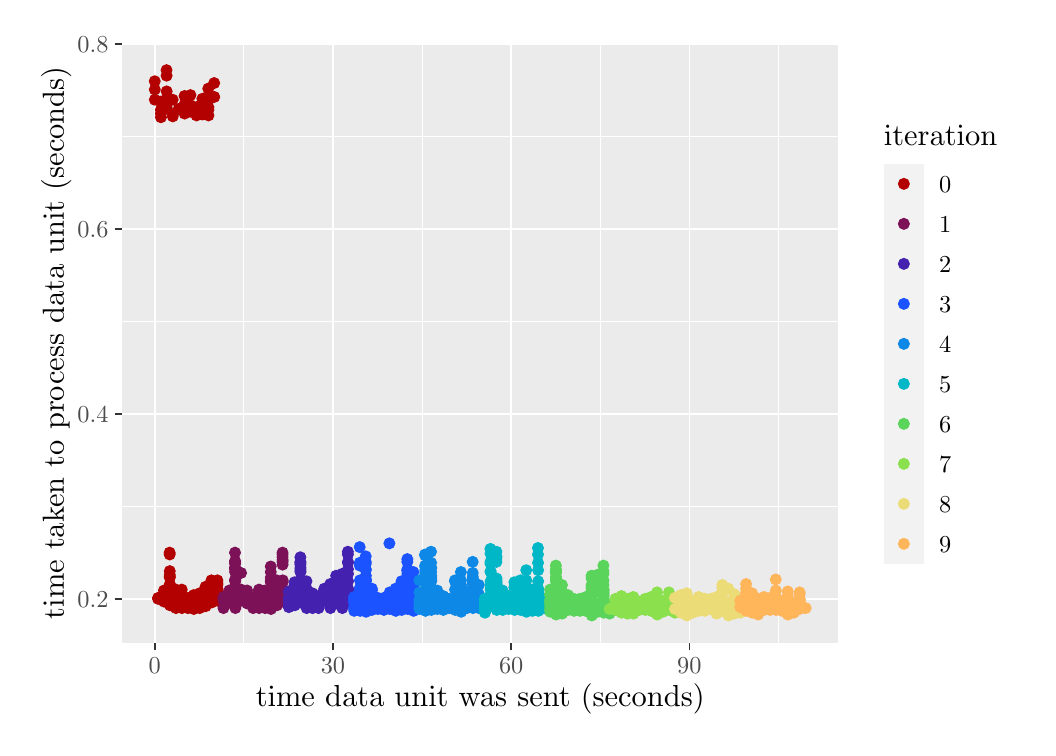
\begin{tikzpicture}[x=1pt,y=1pt]
	\definecolor{fillColor}{RGB}{255,255,255}
	\path[use as bounding box,fill=fillColor,fill opacity=0.00] (0,0) rectangle (361.35,252.94);
	\begin{scope}
	\path[clip] (  0.00,  0.00) rectangle (361.35,252.94);
	\definecolor{drawColor}{RGB}{255,255,255}
	\definecolor{fillColor}{RGB}{255,255,255}
	
	\path[draw=drawColor,line width= 0.6pt,line join=round,line cap=round,fill=fillColor] (  0.00,  0.00) rectangle (361.35,252.94);
	\end{scope}
	\begin{scope}
	\path[clip] ( 34.16, 30.69) rectangle (292.88,247.45);
	\definecolor{fillColor}{gray}{0.92}
	
	\path[fill=fillColor] ( 34.16, 30.69) rectangle (292.88,247.45);
	\definecolor{drawColor}{RGB}{255,255,255}
	
	\path[draw=drawColor,line width= 0.3pt,line join=round] ( 34.16, 79.95) --
		(292.88, 79.95);
	
	\path[draw=drawColor,line width= 0.3pt,line join=round] ( 34.16,146.75) --
		(292.88,146.75);
	
	\path[draw=drawColor,line width= 0.3pt,line join=round] ( 34.16,213.55) --
		(292.88,213.55);
	
	\path[draw=drawColor,line width= 0.3pt,line join=round] ( 78.12, 30.69) --
		( 78.12,247.45);
	
	\path[draw=drawColor,line width= 0.3pt,line join=round] (142.52, 30.69) --
		(142.52,247.45);
	
	\path[draw=drawColor,line width= 0.3pt,line join=round] (206.91, 30.69) --
		(206.91,247.45);
	
	\path[draw=drawColor,line width= 0.3pt,line join=round] (271.31, 30.69) --
		(271.31,247.45);
	
	\path[draw=drawColor,line width= 0.6pt,line join=round] ( 34.16, 46.55) --
		(292.88, 46.55);
	
	\path[draw=drawColor,line width= 0.6pt,line join=round] ( 34.16,113.35) --
		(292.88,113.35);
	
	\path[draw=drawColor,line width= 0.6pt,line join=round] ( 34.16,180.15) --
		(292.88,180.15);
	
	\path[draw=drawColor,line width= 0.6pt,line join=round] ( 34.16,246.94) --
		(292.88,246.94);
	
	\path[draw=drawColor,line width= 0.6pt,line join=round] ( 45.92, 30.69) --
		( 45.92,247.45);
	
	\path[draw=drawColor,line width= 0.6pt,line join=round] (110.32, 30.69) --
		(110.32,247.45);
	
	\path[draw=drawColor,line width= 0.6pt,line join=round] (174.72, 30.69) --
		(174.72,247.45);
	
	\path[draw=drawColor,line width= 0.6pt,line join=round] (239.11, 30.69) --
		(239.11,247.45);
	\definecolor{drawColor}{RGB}{179,0,0}
	\definecolor{fillColor}{RGB}{179,0,0}
	
	\path[draw=drawColor,line width= 0.4pt,line join=round,line cap=round,fill=fillColor] ( 45.92,233.58) circle (  1.96);
	
	\path[draw=drawColor,line width= 0.4pt,line join=round,line cap=round,fill=fillColor] ( 45.96,226.90) circle (  1.96);
	
	\path[draw=drawColor,line width= 0.4pt,line join=round,line cap=round,fill=fillColor] ( 47.12, 46.55) circle (  1.96);
	
	\path[draw=drawColor,line width= 0.4pt,line join=round,line cap=round,fill=fillColor] ( 47.12, 46.88) circle (  1.96);
	
	\path[draw=drawColor,line width= 0.4pt,line join=round,line cap=round,fill=fillColor] ( 45.94,230.58) circle (  1.96);
	
	\path[draw=drawColor,line width= 0.4pt,line join=round,line cap=round,fill=fillColor] ( 49.26, 47.89) circle (  1.96);
	
	\path[draw=drawColor,line width= 0.4pt,line join=round,line cap=round,fill=fillColor] ( 49.27, 46.55) circle (  1.96);
	
	\path[draw=drawColor,line width= 0.4pt,line join=round,line cap=round,fill=fillColor] ( 49.25, 49.56) circle (  1.96);
	
	\path[draw=drawColor,line width= 0.4pt,line join=round,line cap=round,fill=fillColor] ( 48.14,221.89) circle (  1.96);
	
	\path[draw=drawColor,line width= 0.4pt,line join=round,line cap=round,fill=fillColor] ( 48.15,220.56) circle (  1.96);
	
	\path[draw=drawColor,line width= 0.4pt,line join=round,line cap=round,fill=fillColor] ( 49.27, 46.22) circle (  1.96);
	
	\path[draw=drawColor,line width= 0.4pt,line join=round,line cap=round,fill=fillColor] ( 48.13,223.23) circle (  1.96);
	
	\path[draw=drawColor,line width= 0.4pt,line join=round,line cap=round,fill=fillColor] ( 49.27, 45.55) circle (  1.96);
	
	\path[draw=drawColor,line width= 0.4pt,line join=round,line cap=round,fill=fillColor] ( 48.11,226.24) circle (  1.96);
	
	\path[draw=drawColor,line width= 0.4pt,line join=round,line cap=round,fill=fillColor] ( 51.39, 49.89) circle (  1.96);
	
	\path[draw=drawColor,line width= 0.4pt,line join=round,line cap=round,fill=fillColor] ( 50.26,225.90) circle (  1.96);
	
	\path[draw=drawColor,line width= 0.4pt,line join=round,line cap=round,fill=fillColor] ( 51.41, 46.55) circle (  1.96);
	
	\path[draw=drawColor,line width= 0.4pt,line join=round,line cap=round,fill=fillColor] ( 51.41, 46.88) circle (  1.96);
	
	\path[draw=drawColor,line width= 0.4pt,line join=round,line cap=round,fill=fillColor] ( 50.23,229.91) circle (  1.96);
	
	\path[draw=drawColor,line width= 0.4pt,line join=round,line cap=round,fill=fillColor] ( 51.31, 62.58) circle (  1.96);
	
	\path[draw=drawColor,line width= 0.4pt,line join=round,line cap=round,fill=fillColor] ( 51.30, 63.25) circle (  1.96);
	
	\path[draw=drawColor,line width= 0.4pt,line join=round,line cap=round,fill=fillColor] ( 50.18,237.59) circle (  1.96);
	
	\path[draw=drawColor,line width= 0.4pt,line join=round,line cap=round,fill=fillColor] ( 51.35, 56.57) circle (  1.96);
	
	\path[draw=drawColor,line width= 0.4pt,line join=round,line cap=round,fill=fillColor] ( 51.40, 47.89) circle (  1.96);
	
	\path[draw=drawColor,line width= 0.4pt,line join=round,line cap=round,fill=fillColor] ( 51.36, 54.23) circle (  1.96);
	
	\path[draw=drawColor,line width= 0.4pt,line join=round,line cap=round,fill=fillColor] ( 51.36, 54.57) circle (  1.96);
	
	\path[draw=drawColor,line width= 0.4pt,line join=round,line cap=round,fill=fillColor] ( 51.39, 49.56) circle (  1.96);
	
	\path[draw=drawColor,line width= 0.4pt,line join=round,line cap=round,fill=fillColor] ( 50.20,235.59) circle (  1.96);
	
	\path[draw=drawColor,line width= 0.4pt,line join=round,line cap=round,fill=fillColor] ( 51.43, 44.21) circle (  1.96);
	
	\path[draw=drawColor,line width= 0.4pt,line join=round,line cap=round,fill=fillColor] ( 50.25,227.24) circle (  1.96);
	
	\path[draw=drawColor,line width= 0.4pt,line join=round,line cap=round,fill=fillColor] ( 51.36, 55.23) circle (  1.96);
	
	\path[draw=drawColor,line width= 0.4pt,line join=round,line cap=round,fill=fillColor] ( 51.38, 51.89) circle (  1.96);
	
	\path[draw=drawColor,line width= 0.4pt,line join=round,line cap=round,fill=fillColor] ( 51.40, 48.55) circle (  1.96);
	
	\path[draw=drawColor,line width= 0.4pt,line join=round,line cap=round,fill=fillColor] ( 50.27,223.90) circle (  1.96);
	
	\path[draw=drawColor,line width= 0.4pt,line join=round,line cap=round,fill=fillColor] ( 51.39, 50.22) circle (  1.96);
	
	\path[draw=drawColor,line width= 0.4pt,line join=round,line cap=round,fill=fillColor] ( 53.56, 46.22) circle (  1.96);
	
	\path[draw=drawColor,line width= 0.4pt,line join=round,line cap=round,fill=fillColor] ( 53.54, 49.89) circle (  1.96);
	
	\path[draw=drawColor,line width= 0.4pt,line join=round,line cap=round,fill=fillColor] ( 53.56, 46.55) circle (  1.96);
	
	\path[draw=drawColor,line width= 0.4pt,line join=round,line cap=round,fill=fillColor] ( 52.43,221.56) circle (  1.96);
	
	\path[draw=drawColor,line width= 0.4pt,line join=round,line cap=round,fill=fillColor] ( 53.56, 46.88) circle (  1.96);
	
	\path[draw=drawColor,line width= 0.4pt,line join=round,line cap=round,fill=fillColor] ( 52.44,220.89) circle (  1.96);
	
	\path[draw=drawColor,line width= 0.4pt,line join=round,line cap=round,fill=fillColor] ( 53.57, 44.88) circle (  1.96);
	
	\path[draw=drawColor,line width= 0.4pt,line join=round,line cap=round,fill=fillColor] ( 53.56, 45.55) circle (  1.96);
	
	\path[draw=drawColor,line width= 0.4pt,line join=round,line cap=round,fill=fillColor] ( 52.40,226.90) circle (  1.96);
	
	\path[draw=drawColor,line width= 0.4pt,line join=round,line cap=round,fill=fillColor] ( 53.58, 43.21) circle (  1.96);
	
	\path[draw=drawColor,line width= 0.4pt,line join=round,line cap=round,fill=fillColor] ( 55.68, 49.89) circle (  1.96);
	
	\path[draw=drawColor,line width= 0.4pt,line join=round,line cap=round,fill=fillColor] ( 55.70, 47.22) circle (  1.96);
	
	\path[draw=drawColor,line width= 0.4pt,line join=round,line cap=round,fill=fillColor] ( 55.71, 46.55) circle (  1.96);
	
	\path[draw=drawColor,line width= 0.4pt,line join=round,line cap=round,fill=fillColor] ( 55.73, 43.21) circle (  1.96);
	
	\path[draw=drawColor,line width= 0.4pt,line join=round,line cap=round,fill=fillColor] ( 54.57,223.56) circle (  1.96);
	
	\path[draw=drawColor,line width= 0.4pt,line join=round,line cap=round,fill=fillColor] ( 55.70, 46.88) circle (  1.96);
	
	\path[draw=drawColor,line width= 0.4pt,line join=round,line cap=round,fill=fillColor] ( 57.85, 46.55) circle (  1.96);
	
	\path[draw=drawColor,line width= 0.4pt,line join=round,line cap=round,fill=fillColor] ( 56.68,228.24) circle (  1.96);
	
	\path[draw=drawColor,line width= 0.4pt,line join=round,line cap=round,fill=fillColor] ( 56.70,225.23) circle (  1.96);
	
	\path[draw=drawColor,line width= 0.4pt,line join=round,line cap=round,fill=fillColor] ( 56.72,221.89) circle (  1.96);
	
	\path[draw=drawColor,line width= 0.4pt,line join=round,line cap=round,fill=fillColor] ( 57.87, 43.21) circle (  1.96);
	
	\path[draw=drawColor,line width= 0.4pt,line join=round,line cap=round,fill=fillColor] ( 57.85, 46.88) circle (  1.96);
	
	\path[draw=drawColor,line width= 0.4pt,line join=round,line cap=round,fill=fillColor] ( 60.02, 43.21) circle (  1.96);
	
	\path[draw=drawColor,line width= 0.4pt,line join=round,line cap=round,fill=fillColor] ( 60.00, 45.55) circle (  1.96);
	
	\path[draw=drawColor,line width= 0.4pt,line join=round,line cap=round,fill=fillColor] ( 58.83,228.57) circle (  1.96);
	
	\path[draw=drawColor,line width= 0.4pt,line join=round,line cap=round,fill=fillColor] ( 60.00, 46.55) circle (  1.96);
	
	\path[draw=drawColor,line width= 0.4pt,line join=round,line cap=round,fill=fillColor] ( 60.00, 46.22) circle (  1.96);
	
	\path[draw=drawColor,line width= 0.4pt,line join=round,line cap=round,fill=fillColor] ( 59.99, 47.55) circle (  1.96);
	
	\path[draw=drawColor,line width= 0.4pt,line join=round,line cap=round,fill=fillColor] ( 58.87,222.56) circle (  1.96);
	
	\path[draw=drawColor,line width= 0.4pt,line join=round,line cap=round,fill=fillColor] ( 58.85,224.90) circle (  1.96);
	
	\path[draw=drawColor,line width= 0.4pt,line join=round,line cap=round,fill=fillColor] ( 60.02, 42.88) circle (  1.96);
	
	\path[draw=drawColor,line width= 0.4pt,line join=round,line cap=round,fill=fillColor] ( 59.99, 47.89) circle (  1.96);
	
	\path[draw=drawColor,line width= 0.4pt,line join=round,line cap=round,fill=fillColor] ( 60.01, 45.21) circle (  1.96);
	
	\path[draw=drawColor,line width= 0.4pt,line join=round,line cap=round,fill=fillColor] ( 62.14, 46.88) circle (  1.96);
	
	\path[draw=drawColor,line width= 0.4pt,line join=round,line cap=round,fill=fillColor] ( 61.02,221.23) circle (  1.96);
	
	\path[draw=drawColor,line width= 0.4pt,line join=round,line cap=round,fill=fillColor] ( 62.15, 46.55) circle (  1.96);
	
	\path[draw=drawColor,line width= 0.4pt,line join=round,line cap=round,fill=fillColor] ( 61.01,222.56) circle (  1.96);
	
	\path[draw=drawColor,line width= 0.4pt,line join=round,line cap=round,fill=fillColor] ( 62.16, 44.55) circle (  1.96);
	
	\path[draw=drawColor,line width= 0.4pt,line join=round,line cap=round,fill=fillColor] ( 61.00,224.23) circle (  1.96);
	
	\path[draw=drawColor,line width= 0.4pt,line join=round,line cap=round,fill=fillColor] ( 62.15, 45.55) circle (  1.96);
	
	\path[draw=drawColor,line width= 0.4pt,line join=round,line cap=round,fill=fillColor] ( 62.14, 47.89) circle (  1.96);
	
	\path[draw=drawColor,line width= 0.4pt,line join=round,line cap=round,fill=fillColor] ( 62.17, 43.21) circle (  1.96);
	
	\path[draw=drawColor,line width= 0.4pt,line join=round,line cap=round,fill=fillColor] ( 62.13, 48.55) circle (  1.96);
	
	\path[draw=drawColor,line width= 0.4pt,line join=round,line cap=round,fill=fillColor] ( 61.01,223.56) circle (  1.96);
	
	\path[draw=drawColor,line width= 0.4pt,line join=round,line cap=round,fill=fillColor] ( 64.31, 43.88) circle (  1.96);
	
	\path[draw=drawColor,line width= 0.4pt,line join=round,line cap=round,fill=fillColor] ( 64.27, 49.89) circle (  1.96);
	
	\path[draw=drawColor,line width= 0.4pt,line join=round,line cap=round,fill=fillColor] ( 63.13,227.24) circle (  1.96);
	
	\path[draw=drawColor,line width= 0.4pt,line join=round,line cap=round,fill=fillColor] ( 63.14,225.23) circle (  1.96);
	
	\path[draw=drawColor,line width= 0.4pt,line join=round,line cap=round,fill=fillColor] ( 64.28, 47.89) circle (  1.96);
	
	\path[draw=drawColor,line width= 0.4pt,line join=round,line cap=round,fill=fillColor] ( 63.14,225.90) circle (  1.96);
	
	\path[draw=drawColor,line width= 0.4pt,line join=round,line cap=round,fill=fillColor] ( 64.29, 46.88) circle (  1.96);
	
	\path[draw=drawColor,line width= 0.4pt,line join=round,line cap=round,fill=fillColor] ( 64.30, 45.55) circle (  1.96);
	
	\path[draw=drawColor,line width= 0.4pt,line join=round,line cap=round,fill=fillColor] ( 64.27, 49.56) circle (  1.96);
	
	\path[draw=drawColor,line width= 0.4pt,line join=round,line cap=round,fill=fillColor] ( 64.29, 46.55) circle (  1.96);
	
	\path[draw=drawColor,line width= 0.4pt,line join=round,line cap=round,fill=fillColor] ( 64.30, 45.21) circle (  1.96);
	
	\path[draw=drawColor,line width= 0.4pt,line join=round,line cap=round,fill=fillColor] ( 64.26, 50.89) circle (  1.96);
	
	\path[draw=drawColor,line width= 0.4pt,line join=round,line cap=round,fill=fillColor] ( 63.17,221.56) circle (  1.96);
	
	\path[draw=drawColor,line width= 0.4pt,line join=round,line cap=round,fill=fillColor] ( 64.29, 47.55) circle (  1.96);
	
	\path[draw=drawColor,line width= 0.4pt,line join=round,line cap=round,fill=fillColor] ( 64.28, 48.22) circle (  1.96);
	
	\path[draw=drawColor,line width= 0.4pt,line join=round,line cap=round,fill=fillColor] ( 65.30,223.23) circle (  1.96);
	
	\path[draw=drawColor,line width= 0.4pt,line join=round,line cap=round,fill=fillColor] ( 66.44, 46.55) circle (  1.96);
	
	\path[draw=drawColor,line width= 0.4pt,line join=round,line cap=round,fill=fillColor] ( 66.44, 46.22) circle (  1.96);
	
	\path[draw=drawColor,line width= 0.4pt,line join=round,line cap=round,fill=fillColor] ( 66.43, 47.55) circle (  1.96);
	
	\path[draw=drawColor,line width= 0.4pt,line join=round,line cap=round,fill=fillColor] ( 65.32,221.23) circle (  1.96);
	
	\path[draw=drawColor,line width= 0.4pt,line join=round,line cap=round,fill=fillColor] ( 66.42, 49.22) circle (  1.96);
	
	\path[draw=drawColor,line width= 0.4pt,line join=round,line cap=round,fill=fillColor] ( 65.25,230.91) circle (  1.96);
	
	\path[draw=drawColor,line width= 0.4pt,line join=round,line cap=round,fill=fillColor] ( 66.40, 53.23) circle (  1.96);
	
	\path[draw=drawColor,line width= 0.4pt,line join=round,line cap=round,fill=fillColor] ( 66.44, 45.88) circle (  1.96);
	
	\path[draw=drawColor,line width= 0.4pt,line join=round,line cap=round,fill=fillColor] ( 65.28,226.57) circle (  1.96);
	
	\path[draw=drawColor,line width= 0.4pt,line join=round,line cap=round,fill=fillColor] ( 65.27,228.24) circle (  1.96);
	
	\path[draw=drawColor,line width= 0.4pt,line join=round,line cap=round,fill=fillColor] ( 65.30,224.23) circle (  1.96);
	
	\path[draw=drawColor,line width= 0.4pt,line join=round,line cap=round,fill=fillColor] ( 66.45, 45.21) circle (  1.96);
	
	\path[draw=drawColor,line width= 0.4pt,line join=round,line cap=round,fill=fillColor] ( 66.43, 47.22) circle (  1.96);
	
	\path[draw=drawColor,line width= 0.4pt,line join=round,line cap=round,fill=fillColor] ( 66.43, 48.22) circle (  1.96);
	
	\path[draw=drawColor,line width= 0.4pt,line join=round,line cap=round,fill=fillColor] ( 66.42, 49.89) circle (  1.96);
	
	\path[draw=drawColor,line width= 0.4pt,line join=round,line cap=round,fill=fillColor] ( 66.43, 47.89) circle (  1.96);
	
	\path[draw=drawColor,line width= 0.4pt,line join=round,line cap=round,fill=fillColor] ( 68.56, 49.89) circle (  1.96);
	
	\path[draw=drawColor,line width= 0.4pt,line join=round,line cap=round,fill=fillColor] ( 68.55, 51.56) circle (  1.96);
	
	\path[draw=drawColor,line width= 0.4pt,line join=round,line cap=round,fill=fillColor] ( 68.57, 49.22) circle (  1.96);
	
	\path[draw=drawColor,line width= 0.4pt,line join=round,line cap=round,fill=fillColor] ( 68.56, 50.22) circle (  1.96);
	
	\path[draw=drawColor,line width= 0.4pt,line join=round,line cap=round,fill=fillColor] ( 67.42,227.91) circle (  1.96);
	
	\path[draw=drawColor,line width= 0.4pt,line join=round,line cap=round,fill=fillColor] ( 68.59, 46.22) circle (  1.96);
	
	\path[draw=drawColor,line width= 0.4pt,line join=round,line cap=round,fill=fillColor] ( 67.39,232.92) circle (  1.96);
	
	\path[draw=drawColor,line width= 0.4pt,line join=round,line cap=round,fill=fillColor] ( 68.57, 49.56) circle (  1.96);
	
	\path[draw=drawColor,line width= 0.4pt,line join=round,line cap=round,fill=fillColor] ( 68.54, 53.23) circle (  1.96);
	
	\path[draw=drawColor,line width= 0.4pt,line join=round,line cap=round,fill=fillColor] ( 68.57, 48.22) circle (  1.96);
	
	\path[draw=drawColor,line width= 0.4pt,line join=round,line cap=round,fill=fillColor] ( 68.59, 45.88) circle (  1.96);
	
	\path[draw=drawColor,line width= 0.4pt,line join=round,line cap=round,fill=fillColor] ( 68.57, 48.89) circle (  1.96);
	
	\path[draw=drawColor,line width= 0.4pt,line join=round,line cap=round,fill=fillColor] ( 68.55, 52.23) circle (  1.96);
	
	\path[draw=drawColor,line width= 0.4pt,line join=round,line cap=round,fill=fillColor] ( 68.59, 46.55) circle (  1.96);
	
	\path[draw=drawColor,line width= 0.4pt,line join=round,line cap=round,fill=fillColor] ( 68.58, 46.88) circle (  1.96);
	
	\path[draw=drawColor,line width= 0.4pt,line join=round,line cap=round,fill=fillColor] ( 68.58, 47.55) circle (  1.96);
	\definecolor{drawColor}{RGB}{124,17,88}
	\definecolor{fillColor}{RGB}{124,17,88}
	
	\path[draw=drawColor,line width= 0.4pt,line join=round,line cap=round,fill=fillColor] ( 70.73, 46.55) circle (  1.96);
	
	\path[draw=drawColor,line width= 0.4pt,line join=round,line cap=round,fill=fillColor] ( 70.74, 45.88) circle (  1.96);
	
	\path[draw=drawColor,line width= 0.4pt,line join=round,line cap=round,fill=fillColor] ( 70.75, 43.21) circle (  1.96);
	
	\path[draw=drawColor,line width= 0.4pt,line join=round,line cap=round,fill=fillColor] ( 70.73, 47.22) circle (  1.96);
	
	\path[draw=drawColor,line width= 0.4pt,line join=round,line cap=round,fill=fillColor] ( 72.88, 46.22) circle (  1.96);
	
	\path[draw=drawColor,line width= 0.4pt,line join=round,line cap=round,fill=fillColor] ( 72.88, 46.55) circle (  1.96);
	
	\path[draw=drawColor,line width= 0.4pt,line join=round,line cap=round,fill=fillColor] ( 72.87, 47.89) circle (  1.96);
	
	\path[draw=drawColor,line width= 0.4pt,line join=round,line cap=round,fill=fillColor] ( 72.87, 48.22) circle (  1.96);
	
	\path[draw=drawColor,line width= 0.4pt,line join=round,line cap=round,fill=fillColor] ( 72.88, 45.88) circle (  1.96);
	
	\path[draw=drawColor,line width= 0.4pt,line join=round,line cap=round,fill=fillColor] ( 72.89, 45.21) circle (  1.96);
	
	\path[draw=drawColor,line width= 0.4pt,line join=round,line cap=round,fill=fillColor] ( 72.86, 49.56) circle (  1.96);
	
	\path[draw=drawColor,line width= 0.4pt,line join=round,line cap=round,fill=fillColor] ( 75.02, 46.88) circle (  1.96);
	
	\path[draw=drawColor,line width= 0.4pt,line join=round,line cap=round,fill=fillColor] ( 75.01, 48.55) circle (  1.96);
	
	\path[draw=drawColor,line width= 0.4pt,line join=round,line cap=round,fill=fillColor] ( 74.95, 57.91) circle (  1.96);
	
	\path[draw=drawColor,line width= 0.4pt,line join=round,line cap=round,fill=fillColor] ( 74.94, 59.24) circle (  1.96);
	
	\path[draw=drawColor,line width= 0.4pt,line join=round,line cap=round,fill=fillColor] ( 74.92, 63.25) circle (  1.96);
	
	\path[draw=drawColor,line width= 0.4pt,line join=round,line cap=round,fill=fillColor] ( 75.04, 44.88) circle (  1.96);
	
	\path[draw=drawColor,line width= 0.4pt,line join=round,line cap=round,fill=fillColor] ( 75.04, 44.55) circle (  1.96);
	
	\path[draw=drawColor,line width= 0.4pt,line join=round,line cap=round,fill=fillColor] ( 74.96, 57.24) circle (  1.96);
	
	\path[draw=drawColor,line width= 0.4pt,line join=round,line cap=round,fill=fillColor] ( 74.95, 57.57) circle (  1.96);
	
	\path[draw=drawColor,line width= 0.4pt,line join=round,line cap=round,fill=fillColor] ( 74.96, 56.24) circle (  1.96);
	
	\path[draw=drawColor,line width= 0.4pt,line join=round,line cap=round,fill=fillColor] ( 75.01, 49.22) circle (  1.96);
	
	\path[draw=drawColor,line width= 0.4pt,line join=round,line cap=round,fill=fillColor] ( 75.05, 43.21) circle (  1.96);
	
	\path[draw=drawColor,line width= 0.4pt,line join=round,line cap=round,fill=fillColor] ( 75.02, 47.55) circle (  1.96);
	
	\path[draw=drawColor,line width= 0.4pt,line join=round,line cap=round,fill=fillColor] ( 74.98, 52.90) circle (  1.96);
	
	\path[draw=drawColor,line width= 0.4pt,line join=round,line cap=round,fill=fillColor] ( 74.98, 53.23) circle (  1.96);
	
	\path[draw=drawColor,line width= 0.4pt,line join=round,line cap=round,fill=fillColor] ( 74.99, 51.23) circle (  1.96);
	
	\path[draw=drawColor,line width= 0.4pt,line join=round,line cap=round,fill=fillColor] ( 74.98, 53.56) circle (  1.96);
	
	\path[draw=drawColor,line width= 0.4pt,line join=round,line cap=round,fill=fillColor] ( 75.00, 49.89) circle (  1.96);
	
	\path[draw=drawColor,line width= 0.4pt,line join=round,line cap=round,fill=fillColor] ( 75.03, 46.22) circle (  1.96);
	
	\path[draw=drawColor,line width= 0.4pt,line join=round,line cap=round,fill=fillColor] ( 74.94, 60.24) circle (  1.96);
	
	\path[draw=drawColor,line width= 0.4pt,line join=round,line cap=round,fill=fillColor] ( 75.02, 46.55) circle (  1.96);
	
	\path[draw=drawColor,line width= 0.4pt,line join=round,line cap=round,fill=fillColor] ( 75.01, 49.56) circle (  1.96);
	
	\path[draw=drawColor,line width= 0.4pt,line join=round,line cap=round,fill=fillColor] ( 74.94, 59.91) circle (  1.96);
	
	\path[draw=drawColor,line width= 0.4pt,line join=round,line cap=round,fill=fillColor] ( 77.17, 46.22) circle (  1.96);
	
	\path[draw=drawColor,line width= 0.4pt,line join=round,line cap=round,fill=fillColor] ( 77.17, 46.55) circle (  1.96);
	
	\path[draw=drawColor,line width= 0.4pt,line join=round,line cap=round,fill=fillColor] ( 77.15, 49.89) circle (  1.96);
	
	\path[draw=drawColor,line width= 0.4pt,line join=round,line cap=round,fill=fillColor] ( 77.16, 48.55) circle (  1.96);
	
	\path[draw=drawColor,line width= 0.4pt,line join=round,line cap=round,fill=fillColor] ( 77.18, 45.88) circle (  1.96);
	
	\path[draw=drawColor,line width= 0.4pt,line join=round,line cap=round,fill=fillColor] ( 77.15, 49.22) circle (  1.96);
	
	\path[draw=drawColor,line width= 0.4pt,line join=round,line cap=round,fill=fillColor] ( 77.17, 46.88) circle (  1.96);
	
	\path[draw=drawColor,line width= 0.4pt,line join=round,line cap=round,fill=fillColor] ( 77.11, 55.90) circle (  1.96);
	
	\path[draw=drawColor,line width= 0.4pt,line join=round,line cap=round,fill=fillColor] ( 79.32, 46.55) circle (  1.96);
	
	\path[draw=drawColor,line width= 0.4pt,line join=round,line cap=round,fill=fillColor] ( 79.33, 44.88) circle (  1.96);
	
	\path[draw=drawColor,line width= 0.4pt,line join=round,line cap=round,fill=fillColor] ( 79.30, 49.56) circle (  1.96);
	
	\path[draw=drawColor,line width= 0.4pt,line join=round,line cap=round,fill=fillColor] ( 79.32, 45.88) circle (  1.96);
	
	\path[draw=drawColor,line width= 0.4pt,line join=round,line cap=round,fill=fillColor] ( 81.47, 45.88) circle (  1.96);
	
	\path[draw=drawColor,line width= 0.4pt,line join=round,line cap=round,fill=fillColor] ( 81.46, 46.55) circle (  1.96);
	
	\path[draw=drawColor,line width= 0.4pt,line join=round,line cap=round,fill=fillColor] ( 81.49, 43.21) circle (  1.96);
	
	\path[draw=drawColor,line width= 0.4pt,line join=round,line cap=round,fill=fillColor] ( 81.48, 44.21) circle (  1.96);
	
	\path[draw=drawColor,line width= 0.4pt,line join=round,line cap=round,fill=fillColor] ( 81.46, 46.88) circle (  1.96);
	
	\path[draw=drawColor,line width= 0.4pt,line join=round,line cap=round,fill=fillColor] ( 83.61, 46.22) circle (  1.96);
	
	\path[draw=drawColor,line width= 0.4pt,line join=round,line cap=round,fill=fillColor] ( 83.61, 46.55) circle (  1.96);
	
	\path[draw=drawColor,line width= 0.4pt,line join=round,line cap=round,fill=fillColor] ( 83.62, 45.88) circle (  1.96);
	
	\path[draw=drawColor,line width= 0.4pt,line join=round,line cap=round,fill=fillColor] ( 83.60, 47.89) circle (  1.96);
	
	\path[draw=drawColor,line width= 0.4pt,line join=round,line cap=round,fill=fillColor] ( 83.59, 49.22) circle (  1.96);
	
	\path[draw=drawColor,line width= 0.4pt,line join=round,line cap=round,fill=fillColor] ( 83.63, 43.21) circle (  1.96);
	
	\path[draw=drawColor,line width= 0.4pt,line join=round,line cap=round,fill=fillColor] ( 83.59, 49.89) circle (  1.96);
	
	\path[draw=drawColor,line width= 0.4pt,line join=round,line cap=round,fill=fillColor] ( 83.60, 48.22) circle (  1.96);
	
	\path[draw=drawColor,line width= 0.4pt,line join=round,line cap=round,fill=fillColor] ( 85.76, 46.22) circle (  1.96);
	
	\path[draw=drawColor,line width= 0.4pt,line join=round,line cap=round,fill=fillColor] ( 85.76, 46.55) circle (  1.96);
	
	\path[draw=drawColor,line width= 0.4pt,line join=round,line cap=round,fill=fillColor] ( 85.76, 46.88) circle (  1.96);
	
	\path[draw=drawColor,line width= 0.4pt,line join=round,line cap=round,fill=fillColor] ( 85.78, 43.21) circle (  1.96);
	
	\path[draw=drawColor,line width= 0.4pt,line join=round,line cap=round,fill=fillColor] ( 85.74, 49.56) circle (  1.96);
	
	\path[draw=drawColor,line width= 0.4pt,line join=round,line cap=round,fill=fillColor] ( 85.75, 47.22) circle (  1.96);
	
	\path[draw=drawColor,line width= 0.4pt,line join=round,line cap=round,fill=fillColor] ( 85.77, 44.88) circle (  1.96);
	
	\path[draw=drawColor,line width= 0.4pt,line join=round,line cap=round,fill=fillColor] ( 85.75, 47.89) circle (  1.96);
	
	\path[draw=drawColor,line width= 0.4pt,line join=round,line cap=round,fill=fillColor] ( 85.74, 49.22) circle (  1.96);
	
	\path[draw=drawColor,line width= 0.4pt,line join=round,line cap=round,fill=fillColor] ( 87.93, 42.88) circle (  1.96);
	
	\path[draw=drawColor,line width= 0.4pt,line join=round,line cap=round,fill=fillColor] ( 87.89, 48.89) circle (  1.96);
	
	\path[draw=drawColor,line width= 0.4pt,line join=round,line cap=round,fill=fillColor] ( 87.86, 54.23) circle (  1.96);
	
	\path[draw=drawColor,line width= 0.4pt,line join=round,line cap=round,fill=fillColor] ( 87.84, 56.24) circle (  1.96);
	
	\path[draw=drawColor,line width= 0.4pt,line join=round,line cap=round,fill=fillColor] ( 87.89, 48.22) circle (  1.96);
	
	\path[draw=drawColor,line width= 0.4pt,line join=round,line cap=round,fill=fillColor] ( 87.90, 47.89) circle (  1.96);
	
	\path[draw=drawColor,line width= 0.4pt,line join=round,line cap=round,fill=fillColor] ( 87.86, 53.23) circle (  1.96);
	
	\path[draw=drawColor,line width= 0.4pt,line join=round,line cap=round,fill=fillColor] ( 87.86, 52.90) circle (  1.96);
	
	\path[draw=drawColor,line width= 0.4pt,line join=round,line cap=round,fill=fillColor] ( 87.89, 48.55) circle (  1.96);
	
	\path[draw=drawColor,line width= 0.4pt,line join=round,line cap=round,fill=fillColor] ( 87.91, 46.22) circle (  1.96);
	
	\path[draw=drawColor,line width= 0.4pt,line join=round,line cap=round,fill=fillColor] ( 87.88, 49.89) circle (  1.96);
	
	\path[draw=drawColor,line width= 0.4pt,line join=round,line cap=round,fill=fillColor] ( 87.83, 58.24) circle (  1.96);
	
	\path[draw=drawColor,line width= 0.4pt,line join=round,line cap=round,fill=fillColor] ( 87.90, 46.55) circle (  1.96);
	
	\path[draw=drawColor,line width= 0.4pt,line join=round,line cap=round,fill=fillColor] ( 87.88, 50.22) circle (  1.96);
	
	\path[draw=drawColor,line width= 0.4pt,line join=round,line cap=round,fill=fillColor] ( 87.87, 52.56) circle (  1.96);
	
	\path[draw=drawColor,line width= 0.4pt,line join=round,line cap=round,fill=fillColor] ( 90.05, 46.55) circle (  1.96);
	
	\path[draw=drawColor,line width= 0.4pt,line join=round,line cap=round,fill=fillColor] ( 90.03, 49.56) circle (  1.96);
	
	\path[draw=drawColor,line width= 0.4pt,line join=round,line cap=round,fill=fillColor] ( 90.03, 49.89) circle (  1.96);
	
	\path[draw=drawColor,line width= 0.4pt,line join=round,line cap=round,fill=fillColor] ( 90.01, 53.23) circle (  1.96);
	
	\path[draw=drawColor,line width= 0.4pt,line join=round,line cap=round,fill=fillColor] ( 90.06, 45.88) circle (  1.96);
	
	\path[draw=drawColor,line width= 0.4pt,line join=round,line cap=round,fill=fillColor] ( 90.07, 44.21) circle (  1.96);
	
	\path[draw=drawColor,line width= 0.4pt,line join=round,line cap=round,fill=fillColor] ( 90.05, 46.22) circle (  1.96);
	
	\path[draw=drawColor,line width= 0.4pt,line join=round,line cap=round,fill=fillColor] ( 90.04, 48.22) circle (  1.96);
	
	\path[draw=drawColor,line width= 0.4pt,line join=round,line cap=round,fill=fillColor] ( 90.06, 44.88) circle (  1.96);
	
	\path[draw=drawColor,line width= 0.4pt,line join=round,line cap=round,fill=fillColor] ( 90.03, 50.22) circle (  1.96);
	
	\path[draw=drawColor,line width= 0.4pt,line join=round,line cap=round,fill=fillColor] ( 92.20, 46.88) circle (  1.96);
	
	\path[draw=drawColor,line width= 0.4pt,line join=round,line cap=round,fill=fillColor] ( 92.16, 53.23) circle (  1.96);
	
	\path[draw=drawColor,line width= 0.4pt,line join=round,line cap=round,fill=fillColor] ( 92.12, 58.91) circle (  1.96);
	
	\path[draw=drawColor,line width= 0.4pt,line join=round,line cap=round,fill=fillColor] ( 92.10, 61.58) circle (  1.96);
	
	\path[draw=drawColor,line width= 0.4pt,line join=round,line cap=round,fill=fillColor] ( 92.11, 60.58) circle (  1.96);
	
	\path[draw=drawColor,line width= 0.4pt,line join=round,line cap=round,fill=fillColor] ( 92.10, 62.58) circle (  1.96);
	
	\path[draw=drawColor,line width= 0.4pt,line join=round,line cap=round,fill=fillColor] ( 92.18, 49.89) circle (  1.96);
	
	\path[draw=drawColor,line width= 0.4pt,line join=round,line cap=round,fill=fillColor] ( 92.16, 52.56) circle (  1.96);
	
	\path[draw=drawColor,line width= 0.4pt,line join=round,line cap=round,fill=fillColor] ( 92.11, 59.91) circle (  1.96);
	
	\path[draw=drawColor,line width= 0.4pt,line join=round,line cap=round,fill=fillColor] ( 92.09, 63.25) circle (  1.96);
	
	\path[draw=drawColor,line width= 0.4pt,line join=round,line cap=round,fill=fillColor] ( 92.20, 46.22) circle (  1.96);
	
	\path[draw=drawColor,line width= 0.4pt,line join=round,line cap=round,fill=fillColor] ( 92.20, 45.55) circle (  1.96);
	
	\path[draw=drawColor,line width= 0.4pt,line join=round,line cap=round,fill=fillColor] ( 92.20, 46.55) circle (  1.96);
	\definecolor{drawColor}{RGB}{68,33,175}
	\definecolor{fillColor}{RGB}{68,33,175}
	
	\path[draw=drawColor,line width= 0.4pt,line join=round,line cap=round,fill=fillColor] ( 94.33, 49.22) circle (  1.96);
	
	\path[draw=drawColor,line width= 0.4pt,line join=round,line cap=round,fill=fillColor] ( 94.36, 44.88) circle (  1.96);
	
	\path[draw=drawColor,line width= 0.4pt,line join=round,line cap=round,fill=fillColor] ( 94.34, 46.55) circle (  1.96);
	
	\path[draw=drawColor,line width= 0.4pt,line join=round,line cap=round,fill=fillColor] ( 94.36, 43.54) circle (  1.96);
	
	\path[draw=drawColor,line width= 0.4pt,line join=round,line cap=round,fill=fillColor] ( 94.35, 45.88) circle (  1.96);
	
	\path[draw=drawColor,line width= 0.4pt,line join=round,line cap=round,fill=fillColor] ( 94.34, 46.88) circle (  1.96);
	
	\path[draw=drawColor,line width= 0.4pt,line join=round,line cap=round,fill=fillColor] ( 96.49, 46.55) circle (  1.96);
	
	\path[draw=drawColor,line width= 0.4pt,line join=round,line cap=round,fill=fillColor] ( 96.50, 45.88) circle (  1.96);
	
	\path[draw=drawColor,line width= 0.4pt,line join=round,line cap=round,fill=fillColor] ( 96.49, 47.55) circle (  1.96);
	
	\path[draw=drawColor,line width= 0.4pt,line join=round,line cap=round,fill=fillColor] ( 96.47, 49.89) circle (  1.96);
	
	\path[draw=drawColor,line width= 0.4pt,line join=round,line cap=round,fill=fillColor] ( 96.47, 50.22) circle (  1.96);
	
	\path[draw=drawColor,line width= 0.4pt,line join=round,line cap=round,fill=fillColor] ( 96.51, 44.21) circle (  1.96);
	
	\path[draw=drawColor,line width= 0.4pt,line join=round,line cap=round,fill=fillColor] ( 96.50, 45.55) circle (  1.96);
	
	\path[draw=drawColor,line width= 0.4pt,line join=round,line cap=round,fill=fillColor] ( 96.47, 50.56) circle (  1.96);
	
	\path[draw=drawColor,line width= 0.4pt,line join=round,line cap=round,fill=fillColor] ( 96.49, 47.22) circle (  1.96);
	
	\path[draw=drawColor,line width= 0.4pt,line join=round,line cap=round,fill=fillColor] ( 96.46, 51.56) circle (  1.96);
	
	\path[draw=drawColor,line width= 0.4pt,line join=round,line cap=round,fill=fillColor] ( 96.50, 44.88) circle (  1.96);
	
	\path[draw=drawColor,line width= 0.4pt,line join=round,line cap=round,fill=fillColor] ( 96.49, 46.22) circle (  1.96);
	
	\path[draw=drawColor,line width= 0.4pt,line join=round,line cap=round,fill=fillColor] ( 96.45, 52.56) circle (  1.96);
	
	\path[draw=drawColor,line width= 0.4pt,line join=round,line cap=round,fill=fillColor] ( 98.60, 53.23) circle (  1.96);
	
	\path[draw=drawColor,line width= 0.4pt,line join=round,line cap=round,fill=fillColor] ( 98.55, 59.58) circle (  1.96);
	
	\path[draw=drawColor,line width= 0.4pt,line join=round,line cap=round,fill=fillColor] ( 98.54, 61.58) circle (  1.96);
	
	\path[draw=drawColor,line width= 0.4pt,line join=round,line cap=round,fill=fillColor] ( 98.64, 46.55) circle (  1.96);
	
	\path[draw=drawColor,line width= 0.4pt,line join=round,line cap=round,fill=fillColor] ( 98.63, 47.55) circle (  1.96);
	
	\path[draw=drawColor,line width= 0.4pt,line join=round,line cap=round,fill=fillColor] ( 98.57, 56.57) circle (  1.96);
	
	\path[draw=drawColor,line width= 0.4pt,line join=round,line cap=round,fill=fillColor] ( 98.64, 46.22) circle (  1.96);
	
	\path[draw=drawColor,line width= 0.4pt,line join=round,line cap=round,fill=fillColor] ( 98.65, 45.21) circle (  1.96);
	
	\path[draw=drawColor,line width= 0.4pt,line join=round,line cap=round,fill=fillColor] ( 98.58, 56.24) circle (  1.96);
	
	\path[draw=drawColor,line width= 0.4pt,line join=round,line cap=round,fill=fillColor] ( 98.60, 52.23) circle (  1.96);
	
	\path[draw=drawColor,line width= 0.4pt,line join=round,line cap=round,fill=fillColor] ( 98.55, 59.91) circle (  1.96);
	
	\path[draw=drawColor,line width= 0.4pt,line join=round,line cap=round,fill=fillColor] ( 98.62, 49.56) circle (  1.96);
	
	\path[draw=drawColor,line width= 0.4pt,line join=round,line cap=round,fill=fillColor] ( 98.62, 49.89) circle (  1.96);
	
	\path[draw=drawColor,line width= 0.4pt,line join=round,line cap=round,fill=fillColor] ( 98.57, 57.24) circle (  1.96);
	
	\path[draw=drawColor,line width= 0.4pt,line join=round,line cap=round,fill=fillColor] ( 98.56, 58.91) circle (  1.96);
	
	\path[draw=drawColor,line width= 0.4pt,line join=round,line cap=round,fill=fillColor] ( 98.57, 57.91) circle (  1.96);
	
	\path[draw=drawColor,line width= 0.4pt,line join=round,line cap=round,fill=fillColor] ( 98.64, 45.55) circle (  1.96);
	
	\path[draw=drawColor,line width= 0.4pt,line join=round,line cap=round,fill=fillColor] (100.78, 46.55) circle (  1.96);
	
	\path[draw=drawColor,line width= 0.4pt,line join=round,line cap=round,fill=fillColor] (100.74, 52.90) circle (  1.96);
	
	\path[draw=drawColor,line width= 0.4pt,line join=round,line cap=round,fill=fillColor] (100.78, 47.55) circle (  1.96);
	
	\path[draw=drawColor,line width= 0.4pt,line join=round,line cap=round,fill=fillColor] (100.79, 46.22) circle (  1.96);
	
	\path[draw=drawColor,line width= 0.4pt,line join=round,line cap=round,fill=fillColor] (100.77, 48.89) circle (  1.96);
	
	\path[draw=drawColor,line width= 0.4pt,line join=round,line cap=round,fill=fillColor] (100.76, 49.89) circle (  1.96);
	
	\path[draw=drawColor,line width= 0.4pt,line join=round,line cap=round,fill=fillColor] (100.78, 47.22) circle (  1.96);
	
	\path[draw=drawColor,line width= 0.4pt,line join=round,line cap=round,fill=fillColor] (100.79, 45.55) circle (  1.96);
	
	\path[draw=drawColor,line width= 0.4pt,line join=round,line cap=round,fill=fillColor] (100.79, 45.88) circle (  1.96);
	
	\path[draw=drawColor,line width= 0.4pt,line join=round,line cap=round,fill=fillColor] (100.77, 49.56) circle (  1.96);
	
	\path[draw=drawColor,line width= 0.4pt,line join=round,line cap=round,fill=fillColor] (100.81, 43.21) circle (  1.96);
	
	\path[draw=drawColor,line width= 0.4pt,line join=round,line cap=round,fill=fillColor] (100.76, 50.22) circle (  1.96);
	
	\path[draw=drawColor,line width= 0.4pt,line join=round,line cap=round,fill=fillColor] (102.93, 46.55) circle (  1.96);
	
	\path[draw=drawColor,line width= 0.4pt,line join=round,line cap=round,fill=fillColor] (102.95, 43.21) circle (  1.96);
	
	\path[draw=drawColor,line width= 0.4pt,line join=round,line cap=round,fill=fillColor] (102.93, 46.22) circle (  1.96);
	
	\path[draw=drawColor,line width= 0.4pt,line join=round,line cap=round,fill=fillColor] (102.93, 46.88) circle (  1.96);
	
	\path[draw=drawColor,line width= 0.4pt,line join=round,line cap=round,fill=fillColor] (102.92, 48.55) circle (  1.96);
	
	\path[draw=drawColor,line width= 0.4pt,line join=round,line cap=round,fill=fillColor] (102.92, 47.55) circle (  1.96);
	
	\path[draw=drawColor,line width= 0.4pt,line join=round,line cap=round,fill=fillColor] (102.94, 45.88) circle (  1.96);
	
	\path[draw=drawColor,line width= 0.4pt,line join=round,line cap=round,fill=fillColor] (105.08, 46.55) circle (  1.96);
	
	\path[draw=drawColor,line width= 0.4pt,line join=round,line cap=round,fill=fillColor] (105.07, 47.55) circle (  1.96);
	
	\path[draw=drawColor,line width= 0.4pt,line join=round,line cap=round,fill=fillColor] (105.10, 43.54) circle (  1.96);
	
	\path[draw=drawColor,line width= 0.4pt,line join=round,line cap=round,fill=fillColor] (105.08, 45.88) circle (  1.96);
	
	\path[draw=drawColor,line width= 0.4pt,line join=round,line cap=round,fill=fillColor] (105.08, 46.88) circle (  1.96);
	
	\path[draw=drawColor,line width= 0.4pt,line join=round,line cap=round,fill=fillColor] (105.08, 46.22) circle (  1.96);
	
	\path[draw=drawColor,line width= 0.4pt,line join=round,line cap=round,fill=fillColor] (105.10, 43.21) circle (  1.96);
	
	\path[draw=drawColor,line width= 0.4pt,line join=round,line cap=round,fill=fillColor] (105.07, 47.22) circle (  1.96);
	
	\path[draw=drawColor,line width= 0.4pt,line join=round,line cap=round,fill=fillColor] (107.22, 46.55) circle (  1.96);
	
	\path[draw=drawColor,line width= 0.4pt,line join=round,line cap=round,fill=fillColor] (107.22, 47.89) circle (  1.96);
	
	\path[draw=drawColor,line width= 0.4pt,line join=round,line cap=round,fill=fillColor] (107.23, 45.88) circle (  1.96);
	
	\path[draw=drawColor,line width= 0.4pt,line join=round,line cap=round,fill=fillColor] (107.21, 49.56) circle (  1.96);
	
	\path[draw=drawColor,line width= 0.4pt,line join=round,line cap=round,fill=fillColor] (107.21, 48.89) circle (  1.96);
	
	\path[draw=drawColor,line width= 0.4pt,line join=round,line cap=round,fill=fillColor] (107.20, 49.89) circle (  1.96);
	
	\path[draw=drawColor,line width= 0.4pt,line join=round,line cap=round,fill=fillColor] (107.20, 50.22) circle (  1.96);
	
	\path[draw=drawColor,line width= 0.4pt,line join=round,line cap=round,fill=fillColor] (107.23, 46.22) circle (  1.96);
	
	\path[draw=drawColor,line width= 0.4pt,line join=round,line cap=round,fill=fillColor] (109.38, 45.88) circle (  1.96);
	
	\path[draw=drawColor,line width= 0.4pt,line join=round,line cap=round,fill=fillColor] (109.37, 46.22) circle (  1.96);
	
	\path[draw=drawColor,line width= 0.4pt,line join=round,line cap=round,fill=fillColor] (109.39, 43.21) circle (  1.96);
	
	\path[draw=drawColor,line width= 0.4pt,line join=round,line cap=round,fill=fillColor] (109.38, 45.55) circle (  1.96);
	
	\path[draw=drawColor,line width= 0.4pt,line join=round,line cap=round,fill=fillColor] (109.37, 46.55) circle (  1.96);
	
	\path[draw=drawColor,line width= 0.4pt,line join=round,line cap=round,fill=fillColor] (109.38, 44.55) circle (  1.96);
	
	\path[draw=drawColor,line width= 0.4pt,line join=round,line cap=round,fill=fillColor] (109.36, 48.55) circle (  1.96);
	
	\path[draw=drawColor,line width= 0.4pt,line join=round,line cap=round,fill=fillColor] (109.34, 51.56) circle (  1.96);
	
	\path[draw=drawColor,line width= 0.4pt,line join=round,line cap=round,fill=fillColor] (109.34, 51.89) circle (  1.96);
	
	\path[draw=drawColor,line width= 0.4pt,line join=round,line cap=round,fill=fillColor] (109.39, 43.88) circle (  1.96);
	
	\path[draw=drawColor,line width= 0.4pt,line join=round,line cap=round,fill=fillColor] (109.38, 45.21) circle (  1.96);
	
	\path[draw=drawColor,line width= 0.4pt,line join=round,line cap=round,fill=fillColor] (111.50, 49.22) circle (  1.96);
	
	\path[draw=drawColor,line width= 0.4pt,line join=round,line cap=round,fill=fillColor] (111.50, 49.56) circle (  1.96);
	
	\path[draw=drawColor,line width= 0.4pt,line join=round,line cap=round,fill=fillColor] (111.51, 48.22) circle (  1.96);
	
	\path[draw=drawColor,line width= 0.4pt,line join=round,line cap=round,fill=fillColor] (111.49, 51.23) circle (  1.96);
	
	\path[draw=drawColor,line width= 0.4pt,line join=round,line cap=round,fill=fillColor] (111.48, 52.90) circle (  1.96);
	
	\path[draw=drawColor,line width= 0.4pt,line join=round,line cap=round,fill=fillColor] (111.46, 54.90) circle (  1.96);
	
	\path[draw=drawColor,line width= 0.4pt,line join=round,line cap=round,fill=fillColor] (111.52, 46.22) circle (  1.96);
	
	\path[draw=drawColor,line width= 0.4pt,line join=round,line cap=round,fill=fillColor] (111.53, 45.21) circle (  1.96);
	
	\path[draw=drawColor,line width= 0.4pt,line join=round,line cap=round,fill=fillColor] (111.50, 49.89) circle (  1.96);
	
	\path[draw=drawColor,line width= 0.4pt,line join=round,line cap=round,fill=fillColor] (111.51, 48.55) circle (  1.96);
	
	\path[draw=drawColor,line width= 0.4pt,line join=round,line cap=round,fill=fillColor] (111.49, 50.22) circle (  1.96);
	
	\path[draw=drawColor,line width= 0.4pt,line join=round,line cap=round,fill=fillColor] (111.53, 44.88) circle (  1.96);
	
	\path[draw=drawColor,line width= 0.4pt,line join=round,line cap=round,fill=fillColor] (111.52, 45.55) circle (  1.96);
	
	\path[draw=drawColor,line width= 0.4pt,line join=round,line cap=round,fill=fillColor] (111.52, 46.55) circle (  1.96);
	
	\path[draw=drawColor,line width= 0.4pt,line join=round,line cap=round,fill=fillColor] (113.66, 46.55) circle (  1.96);
	
	\path[draw=drawColor,line width= 0.4pt,line join=round,line cap=round,fill=fillColor] (113.67, 45.21) circle (  1.96);
	
	\path[draw=drawColor,line width= 0.4pt,line join=round,line cap=round,fill=fillColor] (113.67, 45.88) circle (  1.96);
	
	\path[draw=drawColor,line width= 0.4pt,line join=round,line cap=round,fill=fillColor] (113.69, 43.21) circle (  1.96);
	
	\path[draw=drawColor,line width= 0.4pt,line join=round,line cap=round,fill=fillColor] (113.66, 47.22) circle (  1.96);
	
	\path[draw=drawColor,line width= 0.4pt,line join=round,line cap=round,fill=fillColor] (113.64, 49.89) circle (  1.96);
	
	\path[draw=drawColor,line width= 0.4pt,line join=round,line cap=round,fill=fillColor] (113.61, 54.57) circle (  1.96);
	
	\path[draw=drawColor,line width= 0.4pt,line join=round,line cap=round,fill=fillColor] (113.67, 46.22) circle (  1.96);
	
	\path[draw=drawColor,line width= 0.4pt,line join=round,line cap=round,fill=fillColor] (113.65, 48.55) circle (  1.96);
	
	\path[draw=drawColor,line width= 0.4pt,line join=round,line cap=round,fill=fillColor] (113.65, 49.56) circle (  1.96);
	
	\path[draw=drawColor,line width= 0.4pt,line join=round,line cap=round,fill=fillColor] (113.63, 52.56) circle (  1.96);
	
	\path[draw=drawColor,line width= 0.4pt,line join=round,line cap=round,fill=fillColor] (113.62, 52.90) circle (  1.96);
	
	\path[draw=drawColor,line width= 0.4pt,line join=round,line cap=round,fill=fillColor] (113.63, 51.89) circle (  1.96);
	
	\path[draw=drawColor,line width= 0.4pt,line join=round,line cap=round,fill=fillColor] (113.65, 49.22) circle (  1.96);
	
	\path[draw=drawColor,line width= 0.4pt,line join=round,line cap=round,fill=fillColor] (113.62, 53.90) circle (  1.96);
	
	\path[draw=drawColor,line width= 0.4pt,line join=round,line cap=round,fill=fillColor] (113.61, 55.57) circle (  1.96);
	
	\path[draw=drawColor,line width= 0.4pt,line join=round,line cap=round,fill=fillColor] (113.65, 48.89) circle (  1.96);
	
	\path[draw=drawColor,line width= 0.4pt,line join=round,line cap=round,fill=fillColor] (113.62, 53.23) circle (  1.96);
	
	\path[draw=drawColor,line width= 0.4pt,line join=round,line cap=round,fill=fillColor] (113.67, 45.55) circle (  1.96);
	
	\path[draw=drawColor,line width= 0.4pt,line join=round,line cap=round,fill=fillColor] (113.65, 48.22) circle (  1.96);
	
	\path[draw=drawColor,line width= 0.4pt,line join=round,line cap=round,fill=fillColor] (115.75, 55.57) circle (  1.96);
	
	\path[draw=drawColor,line width= 0.4pt,line join=round,line cap=round,fill=fillColor] (115.71, 62.58) circle (  1.96);
	
	\path[draw=drawColor,line width= 0.4pt,line join=round,line cap=round,fill=fillColor] (115.73, 59.58) circle (  1.96);
	
	\path[draw=drawColor,line width= 0.4pt,line join=round,line cap=round,fill=fillColor] (115.73, 59.91) circle (  1.96);
	
	\path[draw=drawColor,line width= 0.4pt,line join=round,line cap=round,fill=fillColor] (115.79, 49.56) circle (  1.96);
	
	\path[draw=drawColor,line width= 0.4pt,line join=round,line cap=round,fill=fillColor] (115.79, 50.22) circle (  1.96);
	
	\path[draw=drawColor,line width= 0.4pt,line join=round,line cap=round,fill=fillColor] (115.74, 57.24) circle (  1.96);
	
	\path[draw=drawColor,line width= 0.4pt,line join=round,line cap=round,fill=fillColor] (115.70, 63.58) circle (  1.96);
	
	\path[draw=drawColor,line width= 0.4pt,line join=round,line cap=round,fill=fillColor] (115.77, 52.90) circle (  1.96);
	
	\path[draw=drawColor,line width= 0.4pt,line join=round,line cap=round,fill=fillColor] (115.81, 46.88) circle (  1.96);
	
	\path[draw=drawColor,line width= 0.4pt,line join=round,line cap=round,fill=fillColor] (115.82, 45.21) circle (  1.96);
	
	\path[draw=drawColor,line width= 0.4pt,line join=round,line cap=round,fill=fillColor] (115.82, 45.88) circle (  1.96);
	\definecolor{drawColor}{RGB}{26,83,255}
	\definecolor{fillColor}{RGB}{26,83,255}
	
	\path[draw=drawColor,line width= 0.4pt,line join=round,line cap=round,fill=fillColor] (117.97, 45.21) circle (  1.96);
	
	\path[draw=drawColor,line width= 0.4pt,line join=round,line cap=round,fill=fillColor] (117.99, 42.21) circle (  1.96);
	
	\path[draw=drawColor,line width= 0.4pt,line join=round,line cap=round,fill=fillColor] (117.96, 46.55) circle (  1.96);
	
	\path[draw=drawColor,line width= 0.4pt,line join=round,line cap=round,fill=fillColor] (117.98, 42.88) circle (  1.96);
	
	\path[draw=drawColor,line width= 0.4pt,line join=round,line cap=round,fill=fillColor] (117.96, 46.22) circle (  1.96);
	
	\path[draw=drawColor,line width= 0.4pt,line join=round,line cap=round,fill=fillColor] (117.96, 45.88) circle (  1.96);
	
	\path[draw=drawColor,line width= 0.4pt,line join=round,line cap=round,fill=fillColor] (117.96, 46.88) circle (  1.96);
	
	\path[draw=drawColor,line width= 0.4pt,line join=round,line cap=round,fill=fillColor] (117.95, 47.22) circle (  1.96);
	
	\path[draw=drawColor,line width= 0.4pt,line join=round,line cap=round,fill=fillColor] (117.98, 43.54) circle (  1.96);
	
	\path[draw=drawColor,line width= 0.4pt,line join=round,line cap=round,fill=fillColor] (120.09, 48.55) circle (  1.96);
	
	\path[draw=drawColor,line width= 0.4pt,line join=round,line cap=round,fill=fillColor] (120.06, 53.23) circle (  1.96);
	
	\path[draw=drawColor,line width= 0.4pt,line join=round,line cap=round,fill=fillColor] (120.08, 50.56) circle (  1.96);
	
	\path[draw=drawColor,line width= 0.4pt,line join=round,line cap=round,fill=fillColor] (120.13, 43.21) circle (  1.96);
	
	\path[draw=drawColor,line width= 0.4pt,line join=round,line cap=round,fill=fillColor] (120.10, 46.55) circle (  1.96);
	
	\path[draw=drawColor,line width= 0.4pt,line join=round,line cap=round,fill=fillColor] (120.11, 46.22) circle (  1.96);
	
	\path[draw=drawColor,line width= 0.4pt,line join=round,line cap=round,fill=fillColor] (120.13, 42.21) circle (  1.96);
	
	\path[draw=drawColor,line width= 0.4pt,line join=round,line cap=round,fill=fillColor] (120.08, 50.22) circle (  1.96);
	
	\path[draw=drawColor,line width= 0.4pt,line join=round,line cap=round,fill=fillColor] (120.13, 42.88) circle (  1.96);
	
	\path[draw=drawColor,line width= 0.4pt,line join=round,line cap=round,fill=fillColor] (120.10, 47.89) circle (  1.96);
	
	\path[draw=drawColor,line width= 0.4pt,line join=round,line cap=round,fill=fillColor] (120.10, 46.88) circle (  1.96);
	
	\path[draw=drawColor,line width= 0.4pt,line join=round,line cap=round,fill=fillColor] (120.09, 49.56) circle (  1.96);
	
	\path[draw=drawColor,line width= 0.4pt,line join=round,line cap=round,fill=fillColor] (120.09, 49.22) circle (  1.96);
	
	\path[draw=drawColor,line width= 0.4pt,line join=round,line cap=round,fill=fillColor] (120.02, 59.58) circle (  1.96);
	
	\path[draw=drawColor,line width= 0.4pt,line join=round,line cap=round,fill=fillColor] (120.03, 58.57) circle (  1.96);
	
	\path[draw=drawColor,line width= 0.4pt,line join=round,line cap=round,fill=fillColor] (119.98, 65.25) circle (  1.96);
	
	\path[draw=drawColor,line width= 0.4pt,line join=round,line cap=round,fill=fillColor] (122.28, 41.87) circle (  1.96);
	
	\path[draw=drawColor,line width= 0.4pt,line join=round,line cap=round,fill=fillColor] (122.24, 48.89) circle (  1.96);
	
	\path[draw=drawColor,line width= 0.4pt,line join=round,line cap=round,fill=fillColor] (122.26, 45.21) circle (  1.96);
	
	\path[draw=drawColor,line width= 0.4pt,line join=round,line cap=round,fill=fillColor] (122.23, 49.89) circle (  1.96);
	
	\path[draw=drawColor,line width= 0.4pt,line join=round,line cap=round,fill=fillColor] (122.21, 53.56) circle (  1.96);
	
	\path[draw=drawColor,line width= 0.4pt,line join=round,line cap=round,fill=fillColor] (122.18, 57.24) circle (  1.96);
	
	\path[draw=drawColor,line width= 0.4pt,line join=round,line cap=round,fill=fillColor] (122.26, 45.88) circle (  1.96);
	
	\path[draw=drawColor,line width= 0.4pt,line join=round,line cap=round,fill=fillColor] (122.25, 46.22) circle (  1.96);
	
	\path[draw=drawColor,line width= 0.4pt,line join=round,line cap=round,fill=fillColor] (122.15, 61.91) circle (  1.96);
	
	\path[draw=drawColor,line width= 0.4pt,line join=round,line cap=round,fill=fillColor] (122.21, 53.23) circle (  1.96);
	
	\path[draw=drawColor,line width= 0.4pt,line join=round,line cap=round,fill=fillColor] (122.17, 59.91) circle (  1.96);
	
	\path[draw=drawColor,line width= 0.4pt,line join=round,line cap=round,fill=fillColor] (122.25, 46.55) circle (  1.96);
	
	\path[draw=drawColor,line width= 0.4pt,line join=round,line cap=round,fill=fillColor] (122.24, 47.89) circle (  1.96);
	
	\path[draw=drawColor,line width= 0.4pt,line join=round,line cap=round,fill=fillColor] (122.20, 54.90) circle (  1.96);
	
	\path[draw=drawColor,line width= 0.4pt,line join=round,line cap=round,fill=fillColor] (122.24, 48.55) circle (  1.96);
	
	\path[draw=drawColor,line width= 0.4pt,line join=round,line cap=round,fill=fillColor] (122.27, 42.88) circle (  1.96);
	
	\path[draw=drawColor,line width= 0.4pt,line join=round,line cap=round,fill=fillColor] (122.21, 52.90) circle (  1.96);
	
	\path[draw=drawColor,line width= 0.4pt,line join=round,line cap=round,fill=fillColor] (122.17, 59.24) circle (  1.96);
	
	\path[draw=drawColor,line width= 0.4pt,line join=round,line cap=round,fill=fillColor] (122.18, 56.90) circle (  1.96);
	
	\path[draw=drawColor,line width= 0.4pt,line join=round,line cap=round,fill=fillColor] (122.23, 50.22) circle (  1.96);
	
	\path[draw=drawColor,line width= 0.4pt,line join=round,line cap=round,fill=fillColor] (122.28, 42.21) circle (  1.96);
	
	\path[draw=drawColor,line width= 0.4pt,line join=round,line cap=round,fill=fillColor] (122.25, 47.22) circle (  1.96);
	
	\path[draw=drawColor,line width= 0.4pt,line join=round,line cap=round,fill=fillColor] (124.40, 45.88) circle (  1.96);
	
	\path[draw=drawColor,line width= 0.4pt,line join=round,line cap=round,fill=fillColor] (124.42, 43.21) circle (  1.96);
	
	\path[draw=drawColor,line width= 0.4pt,line join=round,line cap=round,fill=fillColor] (124.37, 50.22) circle (  1.96);
	
	\path[draw=drawColor,line width= 0.4pt,line join=round,line cap=round,fill=fillColor] (124.38, 49.56) circle (  1.96);
	
	\path[draw=drawColor,line width= 0.4pt,line join=round,line cap=round,fill=fillColor] (124.41, 44.88) circle (  1.96);
	
	\path[draw=drawColor,line width= 0.4pt,line join=round,line cap=round,fill=fillColor] (124.40, 46.22) circle (  1.96);
	
	\path[draw=drawColor,line width= 0.4pt,line join=round,line cap=round,fill=fillColor] (124.42, 42.54) circle (  1.96);
	
	\path[draw=drawColor,line width= 0.4pt,line join=round,line cap=round,fill=fillColor] (124.40, 46.88) circle (  1.96);
	
	\path[draw=drawColor,line width= 0.4pt,line join=round,line cap=round,fill=fillColor] (124.40, 46.55) circle (  1.96);
	
	\path[draw=drawColor,line width= 0.4pt,line join=round,line cap=round,fill=fillColor] (124.40, 45.55) circle (  1.96);
	
	\path[draw=drawColor,line width= 0.4pt,line join=round,line cap=round,fill=fillColor] (124.42, 43.54) circle (  1.96);
	
	\path[draw=drawColor,line width= 0.4pt,line join=round,line cap=round,fill=fillColor] (124.39, 48.22) circle (  1.96);
	
	\path[draw=drawColor,line width= 0.4pt,line join=round,line cap=round,fill=fillColor] (126.57, 42.88) circle (  1.96);
	
	\path[draw=drawColor,line width= 0.4pt,line join=round,line cap=round,fill=fillColor] (126.55, 46.22) circle (  1.96);
	
	\path[draw=drawColor,line width= 0.4pt,line join=round,line cap=round,fill=fillColor] (126.54, 46.88) circle (  1.96);
	
	\path[draw=drawColor,line width= 0.4pt,line join=round,line cap=round,fill=fillColor] (126.57, 43.21) circle (  1.96);
	
	\path[draw=drawColor,line width= 0.4pt,line join=round,line cap=round,fill=fillColor] (126.56, 44.55) circle (  1.96);
	
	\path[draw=drawColor,line width= 0.4pt,line join=round,line cap=round,fill=fillColor] (128.70, 45.55) circle (  1.96);
	
	\path[draw=drawColor,line width= 0.4pt,line join=round,line cap=round,fill=fillColor] (128.69, 46.22) circle (  1.96);
	
	\path[draw=drawColor,line width= 0.4pt,line join=round,line cap=round,fill=fillColor] (128.70, 44.88) circle (  1.96);
	
	\path[draw=drawColor,line width= 0.4pt,line join=round,line cap=round,fill=fillColor] (128.70, 45.88) circle (  1.96);
	
	\path[draw=drawColor,line width= 0.4pt,line join=round,line cap=round,fill=fillColor] (128.71, 43.21) circle (  1.96);
	
	\path[draw=drawColor,line width= 0.4pt,line join=round,line cap=round,fill=fillColor] (128.71, 43.54) circle (  1.96);
	
	\path[draw=drawColor,line width= 0.4pt,line join=round,line cap=round,fill=fillColor] (128.69, 46.88) circle (  1.96);
	
	\path[draw=drawColor,line width= 0.4pt,line join=round,line cap=round,fill=fillColor] (128.70, 45.21) circle (  1.96);
	
	\path[draw=drawColor,line width= 0.4pt,line join=round,line cap=round,fill=fillColor] (128.71, 42.88) circle (  1.96);
	
	\path[draw=drawColor,line width= 0.4pt,line join=round,line cap=round,fill=fillColor] (128.69, 46.55) circle (  1.96);
	
	\path[draw=drawColor,line width= 0.4pt,line join=round,line cap=round,fill=fillColor] (128.72, 42.54) circle (  1.96);
	
	\path[draw=drawColor,line width= 0.4pt,line join=round,line cap=round,fill=fillColor] (130.84, 46.22) circle (  1.96);
	
	\path[draw=drawColor,line width= 0.4pt,line join=round,line cap=round,fill=fillColor] (130.86, 43.54) circle (  1.96);
	
	\path[draw=drawColor,line width= 0.4pt,line join=round,line cap=round,fill=fillColor] (130.84, 46.55) circle (  1.96);
	
	\path[draw=drawColor,line width= 0.4pt,line join=round,line cap=round,fill=fillColor] (130.82, 48.89) circle (  1.96);
	
	\path[draw=drawColor,line width= 0.4pt,line join=round,line cap=round,fill=fillColor] (130.86, 42.88) circle (  1.96);
	
	\path[draw=drawColor,line width= 0.4pt,line join=round,line cap=round,fill=fillColor] (130.85, 43.88) circle (  1.96);
	
	\path[draw=drawColor,line width= 0.4pt,line join=round,line cap=round,fill=fillColor] (130.71, 66.59) circle (  1.96);
	
	\path[draw=drawColor,line width= 0.4pt,line join=round,line cap=round,fill=fillColor] (130.86, 43.21) circle (  1.96);
	
	\path[draw=drawColor,line width= 0.4pt,line join=round,line cap=round,fill=fillColor] (130.84, 45.88) circle (  1.96);
	
	\path[draw=drawColor,line width= 0.4pt,line join=round,line cap=round,fill=fillColor] (133.01, 43.21) circle (  1.96);
	
	\path[draw=drawColor,line width= 0.4pt,line join=round,line cap=round,fill=fillColor] (132.99, 45.21) circle (  1.96);
	
	\path[draw=drawColor,line width= 0.4pt,line join=round,line cap=round,fill=fillColor] (133.01, 42.54) circle (  1.96);
	
	\path[draw=drawColor,line width= 0.4pt,line join=round,line cap=round,fill=fillColor] (132.99, 45.88) circle (  1.96);
	
	\path[draw=drawColor,line width= 0.4pt,line join=round,line cap=round,fill=fillColor] (133.00, 43.54) circle (  1.96);
	
	\path[draw=drawColor,line width= 0.4pt,line join=round,line cap=round,fill=fillColor] (132.98, 46.88) circle (  1.96);
	
	\path[draw=drawColor,line width= 0.4pt,line join=round,line cap=round,fill=fillColor] (133.01, 42.21) circle (  1.96);
	
	\path[draw=drawColor,line width= 0.4pt,line join=round,line cap=round,fill=fillColor] (132.96, 50.22) circle (  1.96);
	
	\path[draw=drawColor,line width= 0.4pt,line join=round,line cap=round,fill=fillColor] (132.97, 49.22) circle (  1.96);
	
	\path[draw=drawColor,line width= 0.4pt,line join=round,line cap=round,fill=fillColor] (133.01, 42.88) circle (  1.96);
	
	\path[draw=drawColor,line width= 0.4pt,line join=round,line cap=round,fill=fillColor] (132.99, 45.55) circle (  1.96);
	
	\path[draw=drawColor,line width= 0.4pt,line join=round,line cap=round,fill=fillColor] (133.00, 43.88) circle (  1.96);
	
	\path[draw=drawColor,line width= 0.4pt,line join=round,line cap=round,fill=fillColor] (135.14, 44.88) circle (  1.96);
	
	\path[draw=drawColor,line width= 0.4pt,line join=round,line cap=round,fill=fillColor] (135.13, 46.88) circle (  1.96);
	
	\path[draw=drawColor,line width= 0.4pt,line join=round,line cap=round,fill=fillColor] (135.09, 52.90) circle (  1.96);
	
	\path[draw=drawColor,line width= 0.4pt,line join=round,line cap=round,fill=fillColor] (135.10, 51.23) circle (  1.96);
	
	\path[draw=drawColor,line width= 0.4pt,line join=round,line cap=round,fill=fillColor] (135.13, 46.55) circle (  1.96);
	
	\path[draw=drawColor,line width= 0.4pt,line join=round,line cap=round,fill=fillColor] (135.12, 47.55) circle (  1.96);
	
	\path[draw=drawColor,line width= 0.4pt,line join=round,line cap=round,fill=fillColor] (135.12, 47.89) circle (  1.96);
	
	\path[draw=drawColor,line width= 0.4pt,line join=round,line cap=round,fill=fillColor] (135.12, 48.22) circle (  1.96);
	
	\path[draw=drawColor,line width= 0.4pt,line join=round,line cap=round,fill=fillColor] (135.09, 52.23) circle (  1.96);
	
	\path[draw=drawColor,line width= 0.4pt,line join=round,line cap=round,fill=fillColor] (135.11, 50.56) circle (  1.96);
	
	\path[draw=drawColor,line width= 0.4pt,line join=round,line cap=round,fill=fillColor] (135.10, 51.89) circle (  1.96);
	
	\path[draw=drawColor,line width= 0.4pt,line join=round,line cap=round,fill=fillColor] (135.14, 45.55) circle (  1.96);
	
	\path[draw=drawColor,line width= 0.4pt,line join=round,line cap=round,fill=fillColor] (135.15, 42.88) circle (  1.96);
	
	\path[draw=drawColor,line width= 0.4pt,line join=round,line cap=round,fill=fillColor] (135.13, 47.22) circle (  1.96);
	
	\path[draw=drawColor,line width= 0.4pt,line join=round,line cap=round,fill=fillColor] (135.16, 42.54) circle (  1.96);
	
	\path[draw=drawColor,line width= 0.4pt,line join=round,line cap=round,fill=fillColor] (135.15, 43.21) circle (  1.96);
	
	\path[draw=drawColor,line width= 0.4pt,line join=round,line cap=round,fill=fillColor] (137.30, 43.21) circle (  1.96);
	
	\path[draw=drawColor,line width= 0.4pt,line join=round,line cap=round,fill=fillColor] (137.27, 47.22) circle (  1.96);
	
	\path[draw=drawColor,line width= 0.4pt,line join=round,line cap=round,fill=fillColor] (137.28, 46.55) circle (  1.96);
	
	\path[draw=drawColor,line width= 0.4pt,line join=round,line cap=round,fill=fillColor] (137.28, 46.22) circle (  1.96);
	
	\path[draw=drawColor,line width= 0.4pt,line join=round,line cap=round,fill=fillColor] (137.30, 42.88) circle (  1.96);
	
	\path[draw=drawColor,line width= 0.4pt,line join=round,line cap=round,fill=fillColor] (137.29, 44.55) circle (  1.96);
	
	\path[draw=drawColor,line width= 0.4pt,line join=round,line cap=round,fill=fillColor] (137.26, 49.56) circle (  1.96);
	
	\path[draw=drawColor,line width= 0.4pt,line join=round,line cap=round,fill=fillColor] (137.28, 45.88) circle (  1.96);
	
	\path[draw=drawColor,line width= 0.4pt,line join=round,line cap=round,fill=fillColor] (137.24, 52.23) circle (  1.96);
	
	\path[draw=drawColor,line width= 0.4pt,line join=round,line cap=round,fill=fillColor] (137.25, 50.22) circle (  1.96);
	
	\path[draw=drawColor,line width= 0.4pt,line join=round,line cap=round,fill=fillColor] (137.30, 43.54) circle (  1.96);
	
	\path[draw=drawColor,line width= 0.4pt,line join=round,line cap=round,fill=fillColor] (137.23, 53.23) circle (  1.96);
	
	\path[draw=drawColor,line width= 0.4pt,line join=round,line cap=round,fill=fillColor] (137.27, 47.55) circle (  1.96);
	
	\path[draw=drawColor,line width= 0.4pt,line join=round,line cap=round,fill=fillColor] (137.25, 51.56) circle (  1.96);
	
	\path[draw=drawColor,line width= 0.4pt,line join=round,line cap=round,fill=fillColor] (137.21, 56.90) circle (  1.96);
	
	\path[draw=drawColor,line width= 0.4pt,line join=round,line cap=round,fill=fillColor] (137.21, 57.24) circle (  1.96);
	
	\path[draw=drawColor,line width= 0.4pt,line join=round,line cap=round,fill=fillColor] (137.22, 55.57) circle (  1.96);
	
	\path[draw=drawColor,line width= 0.4pt,line join=round,line cap=round,fill=fillColor] (137.19, 59.91) circle (  1.96);
	
	\path[draw=drawColor,line width= 0.4pt,line join=round,line cap=round,fill=fillColor] (137.19, 60.91) circle (  1.96);
	
	\path[draw=drawColor,line width= 0.4pt,line join=round,line cap=round,fill=fillColor] (137.21, 56.57) circle (  1.96);
	
	\path[draw=drawColor,line width= 0.4pt,line join=round,line cap=round,fill=fillColor] (139.43, 46.22) circle (  1.96);
	
	\path[draw=drawColor,line width= 0.4pt,line join=round,line cap=round,fill=fillColor] (139.42, 46.88) circle (  1.96);
	
	\path[draw=drawColor,line width= 0.4pt,line join=round,line cap=round,fill=fillColor] (139.38, 53.90) circle (  1.96);
	
	\path[draw=drawColor,line width= 0.4pt,line join=round,line cap=round,fill=fillColor] (139.36, 56.24) circle (  1.96);
	
	\path[draw=drawColor,line width= 0.4pt,line join=round,line cap=round,fill=fillColor] (139.40, 50.89) circle (  1.96);
	
	\path[draw=drawColor,line width= 0.4pt,line join=round,line cap=round,fill=fillColor] (139.42, 46.55) circle (  1.96);
	
	\path[draw=drawColor,line width= 0.4pt,line join=round,line cap=round,fill=fillColor] (139.44, 44.55) circle (  1.96);
	
	\path[draw=drawColor,line width= 0.4pt,line join=round,line cap=round,fill=fillColor] (139.45, 43.21) circle (  1.96);
	
	\path[draw=drawColor,line width= 0.4pt,line join=round,line cap=round,fill=fillColor] (139.44, 43.54) circle (  1.96);
	
	\path[draw=drawColor,line width= 0.4pt,line join=round,line cap=round,fill=fillColor] (139.45, 42.21) circle (  1.96);
	\definecolor{drawColor}{RGB}{13,136,230}
	\definecolor{fillColor}{RGB}{13,136,230}
	
	\path[draw=drawColor,line width= 0.4pt,line join=round,line cap=round,fill=fillColor] (141.57, 46.22) circle (  1.96);
	
	\path[draw=drawColor,line width= 0.4pt,line join=round,line cap=round,fill=fillColor] (141.59, 42.88) circle (  1.96);
	
	\path[draw=drawColor,line width= 0.4pt,line join=round,line cap=round,fill=fillColor] (141.59, 44.21) circle (  1.96);
	
	\path[draw=drawColor,line width= 0.4pt,line join=round,line cap=round,fill=fillColor] (141.59, 43.21) circle (  1.96);
	
	\path[draw=drawColor,line width= 0.4pt,line join=round,line cap=round,fill=fillColor] (141.58, 45.55) circle (  1.96);
	
	\path[draw=drawColor,line width= 0.4pt,line join=round,line cap=round,fill=fillColor] (141.58, 45.88) circle (  1.96);
	
	\path[draw=drawColor,line width= 0.4pt,line join=round,line cap=round,fill=fillColor] (141.56, 48.89) circle (  1.96);
	
	\path[draw=drawColor,line width= 0.4pt,line join=round,line cap=round,fill=fillColor] (141.53, 53.23) circle (  1.96);
	
	\path[draw=drawColor,line width= 0.4pt,line join=round,line cap=round,fill=fillColor] (143.73, 43.88) circle (  1.96);
	
	\path[draw=drawColor,line width= 0.4pt,line join=round,line cap=round,fill=fillColor] (143.72, 46.88) circle (  1.96);
	
	\path[draw=drawColor,line width= 0.4pt,line join=round,line cap=round,fill=fillColor] (143.70, 49.22) circle (  1.96);
	
	\path[draw=drawColor,line width= 0.4pt,line join=round,line cap=round,fill=fillColor] (143.73, 44.21) circle (  1.96);
	
	\path[draw=drawColor,line width= 0.4pt,line join=round,line cap=round,fill=fillColor] (143.71, 47.22) circle (  1.96);
	
	\path[draw=drawColor,line width= 0.4pt,line join=round,line cap=round,fill=fillColor] (143.70, 49.89) circle (  1.96);
	
	\path[draw=drawColor,line width= 0.4pt,line join=round,line cap=round,fill=fillColor] (143.75, 42.21) circle (  1.96);
	
	\path[draw=drawColor,line width= 0.4pt,line join=round,line cap=round,fill=fillColor] (143.74, 42.54) circle (  1.96);
	
	\path[draw=drawColor,line width= 0.4pt,line join=round,line cap=round,fill=fillColor] (143.71, 48.22) circle (  1.96);
	
	\path[draw=drawColor,line width= 0.4pt,line join=round,line cap=round,fill=fillColor] (143.73, 44.55) circle (  1.96);
	
	\path[draw=drawColor,line width= 0.4pt,line join=round,line cap=round,fill=fillColor] (143.67, 53.23) circle (  1.96);
	
	\path[draw=drawColor,line width= 0.4pt,line join=round,line cap=round,fill=fillColor] (143.74, 42.88) circle (  1.96);
	
	\path[draw=drawColor,line width= 0.4pt,line join=round,line cap=round,fill=fillColor] (143.64, 58.24) circle (  1.96);
	
	\path[draw=drawColor,line width= 0.4pt,line join=round,line cap=round,fill=fillColor] (143.64, 58.57) circle (  1.96);
	
	\path[draw=drawColor,line width= 0.4pt,line join=round,line cap=round,fill=fillColor] (143.61, 62.58) circle (  1.96);
	
	\path[draw=drawColor,line width= 0.4pt,line join=round,line cap=round,fill=fillColor] (143.62, 62.25) circle (  1.96);
	
	\path[draw=drawColor,line width= 0.4pt,line join=round,line cap=round,fill=fillColor] (143.72, 46.22) circle (  1.96);
	
	\path[draw=drawColor,line width= 0.4pt,line join=round,line cap=round,fill=fillColor] (143.66, 55.90) circle (  1.96);
	
	\path[draw=drawColor,line width= 0.4pt,line join=round,line cap=round,fill=fillColor] (143.65, 56.90) circle (  1.96);
	
	\path[draw=drawColor,line width= 0.4pt,line join=round,line cap=round,fill=fillColor] (145.78, 59.58) circle (  1.96);
	
	\path[draw=drawColor,line width= 0.4pt,line join=round,line cap=round,fill=fillColor] (145.79, 57.57) circle (  1.96);
	
	\path[draw=drawColor,line width= 0.4pt,line join=round,line cap=round,fill=fillColor] (145.89, 42.54) circle (  1.96);
	
	\path[draw=drawColor,line width= 0.4pt,line join=round,line cap=round,fill=fillColor] (145.89, 43.21) circle (  1.96);
	
	\path[draw=drawColor,line width= 0.4pt,line join=round,line cap=round,fill=fillColor] (145.82, 53.23) circle (  1.96);
	
	\path[draw=drawColor,line width= 0.4pt,line join=round,line cap=round,fill=fillColor] (145.82, 53.56) circle (  1.96);
	
	\path[draw=drawColor,line width= 0.4pt,line join=round,line cap=round,fill=fillColor] (145.81, 54.23) circle (  1.96);
	
	\path[draw=drawColor,line width= 0.4pt,line join=round,line cap=round,fill=fillColor] (145.75, 63.58) circle (  1.96);
	
	\path[draw=drawColor,line width= 0.4pt,line join=round,line cap=round,fill=fillColor] (145.79, 57.91) circle (  1.96);
	
	\path[draw=drawColor,line width= 0.4pt,line join=round,line cap=round,fill=fillColor] (145.86, 46.55) circle (  1.96);
	
	\path[draw=drawColor,line width= 0.4pt,line join=round,line cap=round,fill=fillColor] (145.82, 52.90) circle (  1.96);
	
	\path[draw=drawColor,line width= 0.4pt,line join=round,line cap=round,fill=fillColor] (145.80, 56.24) circle (  1.96);
	
	\path[draw=drawColor,line width= 0.4pt,line join=round,line cap=round,fill=fillColor] (145.81, 54.90) circle (  1.96);
	
	\path[draw=drawColor,line width= 0.4pt,line join=round,line cap=round,fill=fillColor] (145.89, 42.88) circle (  1.96);
	
	\path[draw=drawColor,line width= 0.4pt,line join=round,line cap=round,fill=fillColor] (145.86, 47.89) circle (  1.96);
	
	\path[draw=drawColor,line width= 0.4pt,line join=round,line cap=round,fill=fillColor] (145.84, 49.89) circle (  1.96);
	
	\path[draw=drawColor,line width= 0.4pt,line join=round,line cap=round,fill=fillColor] (145.86, 47.22) circle (  1.96);
	
	\path[draw=drawColor,line width= 0.4pt,line join=round,line cap=round,fill=fillColor] (148.02, 45.88) circle (  1.96);
	
	\path[draw=drawColor,line width= 0.4pt,line join=round,line cap=round,fill=fillColor] (147.99, 49.56) circle (  1.96);
	
	\path[draw=drawColor,line width= 0.4pt,line join=round,line cap=round,fill=fillColor] (148.01, 46.55) circle (  1.96);
	
	\path[draw=drawColor,line width= 0.4pt,line join=round,line cap=round,fill=fillColor] (148.03, 43.88) circle (  1.96);
	
	\path[draw=drawColor,line width= 0.4pt,line join=round,line cap=round,fill=fillColor] (148.01, 46.88) circle (  1.96);
	
	\path[draw=drawColor,line width= 0.4pt,line join=round,line cap=round,fill=fillColor] (148.01, 46.22) circle (  1.96);
	
	\path[draw=drawColor,line width= 0.4pt,line join=round,line cap=round,fill=fillColor] (148.03, 42.88) circle (  1.96);
	
	\path[draw=drawColor,line width= 0.4pt,line join=round,line cap=round,fill=fillColor] (148.03, 43.21) circle (  1.96);
	
	\path[draw=drawColor,line width= 0.4pt,line join=round,line cap=round,fill=fillColor] (148.00, 47.55) circle (  1.96);
	
	\path[draw=drawColor,line width= 0.4pt,line join=round,line cap=round,fill=fillColor] (148.03, 44.21) circle (  1.96);
	
	\path[draw=drawColor,line width= 0.4pt,line join=round,line cap=round,fill=fillColor] (148.03, 43.54) circle (  1.96);
	
	\path[draw=drawColor,line width= 0.4pt,line join=round,line cap=round,fill=fillColor] (150.16, 46.88) circle (  1.96);
	
	\path[draw=drawColor,line width= 0.4pt,line join=round,line cap=round,fill=fillColor] (150.17, 45.21) circle (  1.96);
	
	\path[draw=drawColor,line width= 0.4pt,line join=round,line cap=round,fill=fillColor] (150.16, 46.55) circle (  1.96);
	
	\path[draw=drawColor,line width= 0.4pt,line join=round,line cap=round,fill=fillColor] (150.16, 46.22) circle (  1.96);
	
	\path[draw=drawColor,line width= 0.4pt,line join=round,line cap=round,fill=fillColor] (150.17, 43.88) circle (  1.96);
	
	\path[draw=drawColor,line width= 0.4pt,line join=round,line cap=round,fill=fillColor] (150.18, 42.54) circle (  1.96);
	
	\path[draw=drawColor,line width= 0.4pt,line join=round,line cap=round,fill=fillColor] (150.15, 47.55) circle (  1.96);
	
	\path[draw=drawColor,line width= 0.4pt,line join=round,line cap=round,fill=fillColor] (152.31, 45.55) circle (  1.96);
	
	\path[draw=drawColor,line width= 0.4pt,line join=round,line cap=round,fill=fillColor] (152.33, 43.21) circle (  1.96);
	
	\path[draw=drawColor,line width= 0.4pt,line join=round,line cap=round,fill=fillColor] (152.30, 46.55) circle (  1.96);
	
	\path[draw=drawColor,line width= 0.4pt,line join=round,line cap=round,fill=fillColor] (152.32, 44.55) circle (  1.96);
	
	\path[draw=drawColor,line width= 0.4pt,line join=round,line cap=round,fill=fillColor] (152.31, 45.88) circle (  1.96);
	
	\path[draw=drawColor,line width= 0.4pt,line join=round,line cap=round,fill=fillColor] (152.32, 43.88) circle (  1.96);
	
	\path[draw=drawColor,line width= 0.4pt,line join=round,line cap=round,fill=fillColor] (152.32, 43.54) circle (  1.96);
	
	\path[draw=drawColor,line width= 0.4pt,line join=round,line cap=round,fill=fillColor] (154.48, 42.54) circle (  1.96);
	
	\path[draw=drawColor,line width= 0.4pt,line join=round,line cap=round,fill=fillColor] (154.45, 46.55) circle (  1.96);
	
	\path[draw=drawColor,line width= 0.4pt,line join=round,line cap=round,fill=fillColor] (154.41, 52.90) circle (  1.96);
	
	\path[draw=drawColor,line width= 0.4pt,line join=round,line cap=round,fill=fillColor] (154.47, 42.88) circle (  1.96);
	
	\path[draw=drawColor,line width= 0.4pt,line join=round,line cap=round,fill=fillColor] (154.46, 45.55) circle (  1.96);
	
	\path[draw=drawColor,line width= 0.4pt,line join=round,line cap=round,fill=fillColor] (154.43, 49.89) circle (  1.96);
	
	\path[draw=drawColor,line width= 0.4pt,line join=round,line cap=round,fill=fillColor] (154.41, 53.23) circle (  1.96);
	
	\path[draw=drawColor,line width= 0.4pt,line join=round,line cap=round,fill=fillColor] (154.47, 43.21) circle (  1.96);
	
	\path[draw=drawColor,line width= 0.4pt,line join=round,line cap=round,fill=fillColor] (154.46, 44.55) circle (  1.96);
	
	\path[draw=drawColor,line width= 0.4pt,line join=round,line cap=round,fill=fillColor] (154.46, 45.88) circle (  1.96);
	
	\path[draw=drawColor,line width= 0.4pt,line join=round,line cap=round,fill=fillColor] (154.45, 46.22) circle (  1.96);
	
	\path[draw=drawColor,line width= 0.4pt,line join=round,line cap=round,fill=fillColor] (156.60, 46.88) circle (  1.96);
	
	\path[draw=drawColor,line width= 0.4pt,line join=round,line cap=round,fill=fillColor] (156.62, 43.21) circle (  1.96);
	
	\path[draw=drawColor,line width= 0.4pt,line join=round,line cap=round,fill=fillColor] (156.62, 42.54) circle (  1.96);
	
	\path[draw=drawColor,line width= 0.4pt,line join=round,line cap=round,fill=fillColor] (156.58, 49.22) circle (  1.96);
	
	\path[draw=drawColor,line width= 0.4pt,line join=round,line cap=round,fill=fillColor] (156.60, 45.55) circle (  1.96);
	
	\path[draw=drawColor,line width= 0.4pt,line join=round,line cap=round,fill=fillColor] (156.60, 46.55) circle (  1.96);
	
	\path[draw=drawColor,line width= 0.4pt,line join=round,line cap=round,fill=fillColor] (156.59, 47.22) circle (  1.96);
	
	\path[draw=drawColor,line width= 0.4pt,line join=round,line cap=round,fill=fillColor] (156.63, 41.87) circle (  1.96);
	
	\path[draw=drawColor,line width= 0.4pt,line join=round,line cap=round,fill=fillColor] (156.59, 48.22) circle (  1.96);
	
	\path[draw=drawColor,line width= 0.4pt,line join=round,line cap=round,fill=fillColor] (156.62, 42.88) circle (  1.96);
	
	\path[draw=drawColor,line width= 0.4pt,line join=round,line cap=round,fill=fillColor] (156.57, 51.56) circle (  1.96);
	
	\path[draw=drawColor,line width= 0.4pt,line join=round,line cap=round,fill=fillColor] (156.55, 53.23) circle (  1.96);
	
	\path[draw=drawColor,line width= 0.4pt,line join=round,line cap=round,fill=fillColor] (156.60, 46.22) circle (  1.96);
	
	\path[draw=drawColor,line width= 0.4pt,line join=round,line cap=round,fill=fillColor] (156.57, 50.22) circle (  1.96);
	
	\path[draw=drawColor,line width= 0.4pt,line join=round,line cap=round,fill=fillColor] (156.54, 56.24) circle (  1.96);
	
	\path[draw=drawColor,line width= 0.4pt,line join=round,line cap=round,fill=fillColor] (156.57, 50.89) circle (  1.96);
	
	\path[draw=drawColor,line width= 0.4pt,line join=round,line cap=round,fill=fillColor] (158.74, 46.55) circle (  1.96);
	
	\path[draw=drawColor,line width= 0.4pt,line join=round,line cap=round,fill=fillColor] (158.74, 47.89) circle (  1.96);
	
	\path[draw=drawColor,line width= 0.4pt,line join=round,line cap=round,fill=fillColor] (158.75, 45.21) circle (  1.96);
	
	\path[draw=drawColor,line width= 0.4pt,line join=round,line cap=round,fill=fillColor] (158.77, 43.21) circle (  1.96);
	
	\path[draw=drawColor,line width= 0.4pt,line join=round,line cap=round,fill=fillColor] (158.75, 44.88) circle (  1.96);
	
	\path[draw=drawColor,line width= 0.4pt,line join=round,line cap=round,fill=fillColor] (158.73, 48.89) circle (  1.96);
	
	\path[draw=drawColor,line width= 0.4pt,line join=round,line cap=round,fill=fillColor] (158.75, 45.88) circle (  1.96);
	
	\path[draw=drawColor,line width= 0.4pt,line join=round,line cap=round,fill=fillColor] (158.75, 46.22) circle (  1.96);
	
	\path[draw=drawColor,line width= 0.4pt,line join=round,line cap=round,fill=fillColor] (158.73, 48.22) circle (  1.96);
	
	\path[draw=drawColor,line width= 0.4pt,line join=round,line cap=round,fill=fillColor] (158.75, 45.55) circle (  1.96);
	
	\path[draw=drawColor,line width= 0.4pt,line join=round,line cap=round,fill=fillColor] (158.74, 47.55) circle (  1.96);
	
	\path[draw=drawColor,line width= 0.4pt,line join=round,line cap=round,fill=fillColor] (158.76, 44.21) circle (  1.96);
	
	\path[draw=drawColor,line width= 0.4pt,line join=round,line cap=round,fill=fillColor] (160.89, 46.22) circle (  1.96);
	
	\path[draw=drawColor,line width= 0.4pt,line join=round,line cap=round,fill=fillColor] (160.88, 48.22) circle (  1.96);
	
	\path[draw=drawColor,line width= 0.4pt,line join=round,line cap=round,fill=fillColor] (160.89, 46.55) circle (  1.96);
	
	\path[draw=drawColor,line width= 0.4pt,line join=round,line cap=round,fill=fillColor] (160.91, 43.21) circle (  1.96);
	
	\path[draw=drawColor,line width= 0.4pt,line join=round,line cap=round,fill=fillColor] (160.91, 43.54) circle (  1.96);
	
	\path[draw=drawColor,line width= 0.4pt,line join=round,line cap=round,fill=fillColor] (160.85, 52.56) circle (  1.96);
	
	\path[draw=drawColor,line width= 0.4pt,line join=round,line cap=round,fill=fillColor] (160.80, 59.91) circle (  1.96);
	
	\path[draw=drawColor,line width= 0.4pt,line join=round,line cap=round,fill=fillColor] (160.84, 54.57) circle (  1.96);
	
	\path[draw=drawColor,line width= 0.4pt,line join=round,line cap=round,fill=fillColor] (160.90, 45.55) circle (  1.96);
	
	\path[draw=drawColor,line width= 0.4pt,line join=round,line cap=round,fill=fillColor] (160.87, 50.22) circle (  1.96);
	
	\path[draw=drawColor,line width= 0.4pt,line join=round,line cap=round,fill=fillColor] (160.85, 53.56) circle (  1.96);
	
	\path[draw=drawColor,line width= 0.4pt,line join=round,line cap=round,fill=fillColor] (160.88, 48.55) circle (  1.96);
	
	\path[draw=drawColor,line width= 0.4pt,line join=round,line cap=round,fill=fillColor] (160.86, 51.89) circle (  1.96);
	
	\path[draw=drawColor,line width= 0.4pt,line join=round,line cap=round,fill=fillColor] (160.87, 49.56) circle (  1.96);
	
	\path[draw=drawColor,line width= 0.4pt,line join=round,line cap=round,fill=fillColor] (160.83, 55.90) circle (  1.96);
	
	\path[draw=drawColor,line width= 0.4pt,line join=round,line cap=round,fill=fillColor] (160.87, 50.56) circle (  1.96);
	
	\path[draw=drawColor,line width= 0.4pt,line join=round,line cap=round,fill=fillColor] (160.90, 45.88) circle (  1.96);
	
	\path[draw=drawColor,line width= 0.4pt,line join=round,line cap=round,fill=fillColor] (160.88, 48.89) circle (  1.96);
	
	\path[draw=drawColor,line width= 0.4pt,line join=round,line cap=round,fill=fillColor] (160.84, 53.90) circle (  1.96);
	
	\path[draw=drawColor,line width= 0.4pt,line join=round,line cap=round,fill=fillColor] (160.91, 43.88) circle (  1.96);
	
	\path[draw=drawColor,line width= 0.4pt,line join=round,line cap=round,fill=fillColor] (163.01, 51.56) circle (  1.96);
	
	\path[draw=drawColor,line width= 0.4pt,line join=round,line cap=round,fill=fillColor] (163.06, 43.54) circle (  1.96);
	
	\path[draw=drawColor,line width= 0.4pt,line join=round,line cap=round,fill=fillColor] (163.04, 45.55) circle (  1.96);
	
	\path[draw=drawColor,line width= 0.4pt,line join=round,line cap=round,fill=fillColor] (163.06, 43.21) circle (  1.96);
	
	\path[draw=drawColor,line width= 0.4pt,line join=round,line cap=round,fill=fillColor] (163.04, 46.22) circle (  1.96);
	
	\path[draw=drawColor,line width= 0.4pt,line join=round,line cap=round,fill=fillColor] (163.04, 46.55) circle (  1.96);
	
	\path[draw=drawColor,line width= 0.4pt,line join=round,line cap=round,fill=fillColor] (163.03, 48.22) circle (  1.96);
	\definecolor{drawColor}{RGB}{0,183,199}
	\definecolor{fillColor}{RGB}{0,183,199}
	
	\path[draw=drawColor,line width= 0.4pt,line join=round,line cap=round,fill=fillColor] (165.21, 43.21) circle (  1.96);
	
	\path[draw=drawColor,line width= 0.4pt,line join=round,line cap=round,fill=fillColor] (165.22, 41.54) circle (  1.96);
	
	\path[draw=drawColor,line width= 0.4pt,line join=round,line cap=round,fill=fillColor] (165.20, 43.88) circle (  1.96);
	
	\path[draw=drawColor,line width= 0.4pt,line join=round,line cap=round,fill=fillColor] (165.21, 41.87) circle (  1.96);
	
	\path[draw=drawColor,line width= 0.4pt,line join=round,line cap=round,fill=fillColor] (165.19, 46.22) circle (  1.96);
	
	\path[draw=drawColor,line width= 0.4pt,line join=round,line cap=round,fill=fillColor] (165.20, 43.54) circle (  1.96);
	
	\path[draw=drawColor,line width= 0.4pt,line join=round,line cap=round,fill=fillColor] (165.19, 44.88) circle (  1.96);
	
	\path[draw=drawColor,line width= 0.4pt,line join=round,line cap=round,fill=fillColor] (165.18, 46.55) circle (  1.96);
	
	\path[draw=drawColor,line width= 0.4pt,line join=round,line cap=round,fill=fillColor] (167.33, 46.55) circle (  1.96);
	
	\path[draw=drawColor,line width= 0.4pt,line join=round,line cap=round,fill=fillColor] (167.32, 48.22) circle (  1.96);
	
	\path[draw=drawColor,line width= 0.4pt,line join=round,line cap=round,fill=fillColor] (167.35, 43.88) circle (  1.96);
	
	\path[draw=drawColor,line width= 0.4pt,line join=round,line cap=round,fill=fillColor] (167.33, 46.88) circle (  1.96);
	
	\path[draw=drawColor,line width= 0.4pt,line join=round,line cap=round,fill=fillColor] (167.30, 51.23) circle (  1.96);
	
	\path[draw=drawColor,line width= 0.4pt,line join=round,line cap=round,fill=fillColor] (167.34, 45.88) circle (  1.96);
	
	\path[draw=drawColor,line width= 0.4pt,line join=round,line cap=round,fill=fillColor] (167.31, 49.89) circle (  1.96);
	
	\path[draw=drawColor,line width= 0.4pt,line join=round,line cap=round,fill=fillColor] (167.29, 52.90) circle (  1.96);
	
	\path[draw=drawColor,line width= 0.4pt,line join=round,line cap=round,fill=fillColor] (167.31, 50.22) circle (  1.96);
	
	\path[draw=drawColor,line width= 0.4pt,line join=round,line cap=round,fill=fillColor] (167.34, 44.55) circle (  1.96);
	
	\path[draw=drawColor,line width= 0.4pt,line join=round,line cap=round,fill=fillColor] (167.33, 47.22) circle (  1.96);
	
	\path[draw=drawColor,line width= 0.4pt,line join=round,line cap=round,fill=fillColor] (167.30, 51.89) circle (  1.96);
	
	\path[draw=drawColor,line width= 0.4pt,line join=round,line cap=round,fill=fillColor] (167.25, 59.24) circle (  1.96);
	
	\path[draw=drawColor,line width= 0.4pt,line join=round,line cap=round,fill=fillColor] (167.27, 56.24) circle (  1.96);
	
	\path[draw=drawColor,line width= 0.4pt,line join=round,line cap=round,fill=fillColor] (167.24, 59.91) circle (  1.96);
	
	\path[draw=drawColor,line width= 0.4pt,line join=round,line cap=round,fill=fillColor] (167.21, 64.59) circle (  1.96);
	
	\path[draw=drawColor,line width= 0.4pt,line join=round,line cap=round,fill=fillColor] (167.27, 56.57) circle (  1.96);
	
	\path[draw=drawColor,line width= 0.4pt,line join=round,line cap=round,fill=fillColor] (167.23, 62.92) circle (  1.96);
	
	\path[draw=drawColor,line width= 0.4pt,line join=round,line cap=round,fill=fillColor] (169.48, 46.55) circle (  1.96);
	
	\path[draw=drawColor,line width= 0.4pt,line join=round,line cap=round,fill=fillColor] (169.43, 53.90) circle (  1.96);
	
	\path[draw=drawColor,line width= 0.4pt,line join=round,line cap=round,fill=fillColor] (169.39, 59.91) circle (  1.96);
	
	\path[draw=drawColor,line width= 0.4pt,line join=round,line cap=round,fill=fillColor] (169.38, 61.25) circle (  1.96);
	
	\path[draw=drawColor,line width= 0.4pt,line join=round,line cap=round,fill=fillColor] (169.37, 63.58) circle (  1.96);
	
	\path[draw=drawColor,line width= 0.4pt,line join=round,line cap=round,fill=fillColor] (169.47, 47.22) circle (  1.96);
	
	\path[draw=drawColor,line width= 0.4pt,line join=round,line cap=round,fill=fillColor] (169.46, 48.55) circle (  1.96);
	
	\path[draw=drawColor,line width= 0.4pt,line join=round,line cap=round,fill=fillColor] (169.44, 51.89) circle (  1.96);
	
	\path[draw=drawColor,line width= 0.4pt,line join=round,line cap=round,fill=fillColor] (169.43, 53.23) circle (  1.96);
	
	\path[draw=drawColor,line width= 0.4pt,line join=round,line cap=round,fill=fillColor] (169.48, 45.55) circle (  1.96);
	
	\path[draw=drawColor,line width= 0.4pt,line join=round,line cap=round,fill=fillColor] (169.44, 52.56) circle (  1.96);
	
	\path[draw=drawColor,line width= 0.4pt,line join=round,line cap=round,fill=fillColor] (169.38, 61.91) circle (  1.96);
	
	\path[draw=drawColor,line width= 0.4pt,line join=round,line cap=round,fill=fillColor] (169.48, 46.88) circle (  1.96);
	
	\path[draw=drawColor,line width= 0.4pt,line join=round,line cap=round,fill=fillColor] (169.50, 42.88) circle (  1.96);
	
	\path[draw=drawColor,line width= 0.4pt,line join=round,line cap=round,fill=fillColor] (169.46, 49.89) circle (  1.96);
	
	\path[draw=drawColor,line width= 0.4pt,line join=round,line cap=round,fill=fillColor] (169.50, 42.54) circle (  1.96);
	
	\path[draw=drawColor,line width= 0.4pt,line join=round,line cap=round,fill=fillColor] (171.62, 46.55) circle (  1.96);
	
	\path[draw=drawColor,line width= 0.4pt,line join=round,line cap=round,fill=fillColor] (171.65, 43.21) circle (  1.96);
	
	\path[draw=drawColor,line width= 0.4pt,line join=round,line cap=round,fill=fillColor] (171.60, 49.56) circle (  1.96);
	
	\path[draw=drawColor,line width= 0.4pt,line join=round,line cap=round,fill=fillColor] (171.64, 44.55) circle (  1.96);
	
	\path[draw=drawColor,line width= 0.4pt,line join=round,line cap=round,fill=fillColor] (171.65, 42.54) circle (  1.96);
	
	\path[draw=drawColor,line width= 0.4pt,line join=round,line cap=round,fill=fillColor] (171.63, 46.22) circle (  1.96);
	
	\path[draw=drawColor,line width= 0.4pt,line join=round,line cap=round,fill=fillColor] (171.62, 47.22) circle (  1.96);
	
	\path[draw=drawColor,line width= 0.4pt,line join=round,line cap=round,fill=fillColor] (171.62, 46.88) circle (  1.96);
	
	\path[draw=drawColor,line width= 0.4pt,line join=round,line cap=round,fill=fillColor] (171.62, 47.55) circle (  1.96);
	
	\path[draw=drawColor,line width= 0.4pt,line join=round,line cap=round,fill=fillColor] (171.65, 42.88) circle (  1.96);
	
	\path[draw=drawColor,line width= 0.4pt,line join=round,line cap=round,fill=fillColor] (171.63, 45.88) circle (  1.96);
	
	\path[draw=drawColor,line width= 0.4pt,line join=round,line cap=round,fill=fillColor] (173.79, 43.21) circle (  1.96);
	
	\path[draw=drawColor,line width= 0.4pt,line join=round,line cap=round,fill=fillColor] (173.76, 47.55) circle (  1.96);
	
	\path[draw=drawColor,line width= 0.4pt,line join=round,line cap=round,fill=fillColor] (173.77, 46.55) circle (  1.96);
	
	\path[draw=drawColor,line width= 0.4pt,line join=round,line cap=round,fill=fillColor] (173.79, 42.88) circle (  1.96);
	
	\path[draw=drawColor,line width= 0.4pt,line join=round,line cap=round,fill=fillColor] (173.77, 45.88) circle (  1.96);
	
	\path[draw=drawColor,line width= 0.4pt,line join=round,line cap=round,fill=fillColor] (175.94, 42.88) circle (  1.96);
	
	\path[draw=drawColor,line width= 0.4pt,line join=round,line cap=round,fill=fillColor] (175.89, 50.89) circle (  1.96);
	
	\path[draw=drawColor,line width= 0.4pt,line join=round,line cap=round,fill=fillColor] (175.94, 43.21) circle (  1.96);
	
	\path[draw=drawColor,line width= 0.4pt,line join=round,line cap=round,fill=fillColor] (175.92, 46.55) circle (  1.96);
	
	\path[draw=drawColor,line width= 0.4pt,line join=round,line cap=round,fill=fillColor] (175.92, 46.88) circle (  1.96);
	
	\path[draw=drawColor,line width= 0.4pt,line join=round,line cap=round,fill=fillColor] (175.92, 45.55) circle (  1.96);
	
	\path[draw=drawColor,line width= 0.4pt,line join=round,line cap=round,fill=fillColor] (175.93, 43.88) circle (  1.96);
	
	\path[draw=drawColor,line width= 0.4pt,line join=round,line cap=round,fill=fillColor] (175.89, 50.56) circle (  1.96);
	
	\path[draw=drawColor,line width= 0.4pt,line join=round,line cap=round,fill=fillColor] (175.88, 52.56) circle (  1.96);
	
	\path[draw=drawColor,line width= 0.4pt,line join=round,line cap=round,fill=fillColor] (175.94, 42.54) circle (  1.96);
	
	\path[draw=drawColor,line width= 0.4pt,line join=round,line cap=round,fill=fillColor] (175.92, 46.22) circle (  1.96);
	
	\path[draw=drawColor,line width= 0.4pt,line join=round,line cap=round,fill=fillColor] (178.02, 53.23) circle (  1.96);
	
	\path[draw=drawColor,line width= 0.4pt,line join=round,line cap=round,fill=fillColor] (178.09, 43.21) circle (  1.96);
	
	\path[draw=drawColor,line width= 0.4pt,line join=round,line cap=round,fill=fillColor] (178.04, 50.22) circle (  1.96);
	
	\path[draw=drawColor,line width= 0.4pt,line join=round,line cap=round,fill=fillColor] (178.04, 49.89) circle (  1.96);
	
	\path[draw=drawColor,line width= 0.4pt,line join=round,line cap=round,fill=fillColor] (178.06, 46.55) circle (  1.96);
	
	\path[draw=drawColor,line width= 0.4pt,line join=round,line cap=round,fill=fillColor] (178.09, 42.88) circle (  1.96);
	
	\path[draw=drawColor,line width= 0.4pt,line join=round,line cap=round,fill=fillColor] (178.08, 44.21) circle (  1.96);
	
	\path[draw=drawColor,line width= 0.4pt,line join=round,line cap=round,fill=fillColor] (178.09, 42.54) circle (  1.96);
	
	\path[draw=drawColor,line width= 0.4pt,line join=round,line cap=round,fill=fillColor] (178.08, 43.54) circle (  1.96);
	
	\path[draw=drawColor,line width= 0.4pt,line join=round,line cap=round,fill=fillColor] (180.21, 46.55) circle (  1.96);
	
	\path[draw=drawColor,line width= 0.4pt,line join=round,line cap=round,fill=fillColor] (180.21, 45.88) circle (  1.96);
	
	\path[draw=drawColor,line width= 0.4pt,line join=round,line cap=round,fill=fillColor] (180.21, 46.22) circle (  1.96);
	
	\path[draw=drawColor,line width= 0.4pt,line join=round,line cap=round,fill=fillColor] (180.23, 42.88) circle (  1.96);
	
	\path[draw=drawColor,line width= 0.4pt,line join=round,line cap=round,fill=fillColor] (180.23, 43.54) circle (  1.96);
	
	\path[draw=drawColor,line width= 0.4pt,line join=round,line cap=round,fill=fillColor] (180.23, 43.21) circle (  1.96);
	
	\path[draw=drawColor,line width= 0.4pt,line join=round,line cap=round,fill=fillColor] (180.19, 49.22) circle (  1.96);
	
	\path[draw=drawColor,line width= 0.4pt,line join=round,line cap=round,fill=fillColor] (180.14, 56.90) circle (  1.96);
	
	\path[draw=drawColor,line width= 0.4pt,line join=round,line cap=round,fill=fillColor] (180.24, 41.87) circle (  1.96);
	
	\path[draw=drawColor,line width= 0.4pt,line join=round,line cap=round,fill=fillColor] (180.19, 50.22) circle (  1.96);
	
	\path[draw=drawColor,line width= 0.4pt,line join=round,line cap=round,fill=fillColor] (180.20, 47.89) circle (  1.96);
	
	\path[draw=drawColor,line width= 0.4pt,line join=round,line cap=round,fill=fillColor] (180.19, 49.56) circle (  1.96);
	
	\path[draw=drawColor,line width= 0.4pt,line join=round,line cap=round,fill=fillColor] (180.17, 53.23) circle (  1.96);
	
	\path[draw=drawColor,line width= 0.4pt,line join=round,line cap=round,fill=fillColor] (180.20, 48.55) circle (  1.96);
	
	\path[draw=drawColor,line width= 0.4pt,line join=round,line cap=round,fill=fillColor] (180.22, 44.55) circle (  1.96);
	
	\path[draw=drawColor,line width= 0.4pt,line join=round,line cap=round,fill=fillColor] (182.36, 46.22) circle (  1.96);
	
	\path[draw=drawColor,line width= 0.4pt,line join=round,line cap=round,fill=fillColor] (182.36, 46.55) circle (  1.96);
	
	\path[draw=drawColor,line width= 0.4pt,line join=round,line cap=round,fill=fillColor] (182.35, 47.55) circle (  1.96);
	
	\path[draw=drawColor,line width= 0.4pt,line join=round,line cap=round,fill=fillColor] (182.38, 43.21) circle (  1.96);
	
	\path[draw=drawColor,line width= 0.4pt,line join=round,line cap=round,fill=fillColor] (182.37, 45.21) circle (  1.96);
	
	\path[draw=drawColor,line width= 0.4pt,line join=round,line cap=round,fill=fillColor] (182.34, 49.22) circle (  1.96);
	
	\path[draw=drawColor,line width= 0.4pt,line join=round,line cap=round,fill=fillColor] (182.35, 47.89) circle (  1.96);
	
	\path[draw=drawColor,line width= 0.4pt,line join=round,line cap=round,fill=fillColor] (182.34, 49.89) circle (  1.96);
	
	\path[draw=drawColor,line width= 0.4pt,line join=round,line cap=round,fill=fillColor] (182.39, 42.21) circle (  1.96);
	
	\path[draw=drawColor,line width= 0.4pt,line join=round,line cap=round,fill=fillColor] (182.37, 44.88) circle (  1.96);
	
	\path[draw=drawColor,line width= 0.4pt,line join=round,line cap=round,fill=fillColor] (182.36, 46.88) circle (  1.96);
	
	\path[draw=drawColor,line width= 0.4pt,line join=round,line cap=round,fill=fillColor] (182.35, 48.22) circle (  1.96);
	
	\path[draw=drawColor,line width= 0.4pt,line join=round,line cap=round,fill=fillColor] (184.48, 49.89) circle (  1.96);
	
	\path[draw=drawColor,line width= 0.4pt,line join=round,line cap=round,fill=fillColor] (184.51, 45.55) circle (  1.96);
	
	\path[draw=drawColor,line width= 0.4pt,line join=round,line cap=round,fill=fillColor] (184.53, 42.21) circle (  1.96);
	
	\path[draw=drawColor,line width= 0.4pt,line join=round,line cap=round,fill=fillColor] (184.51, 45.21) circle (  1.96);
	
	\path[draw=drawColor,line width= 0.4pt,line join=round,line cap=round,fill=fillColor] (184.50, 47.89) circle (  1.96);
	
	\path[draw=drawColor,line width= 0.4pt,line join=round,line cap=round,fill=fillColor] (184.49, 49.22) circle (  1.96);
	
	\path[draw=drawColor,line width= 0.4pt,line join=round,line cap=round,fill=fillColor] (184.48, 49.56) circle (  1.96);
	
	\path[draw=drawColor,line width= 0.4pt,line join=round,line cap=round,fill=fillColor] (184.46, 52.90) circle (  1.96);
	
	\path[draw=drawColor,line width= 0.4pt,line join=round,line cap=round,fill=fillColor] (184.53, 43.21) circle (  1.96);
	
	\path[draw=drawColor,line width= 0.4pt,line join=round,line cap=round,fill=fillColor] (184.50, 46.55) circle (  1.96);
	
	\path[draw=drawColor,line width= 0.4pt,line join=round,line cap=round,fill=fillColor] (184.49, 48.55) circle (  1.96);
	
	\path[draw=drawColor,line width= 0.4pt,line join=round,line cap=round,fill=fillColor] (184.50, 47.22) circle (  1.96);
	
	\path[draw=drawColor,line width= 0.4pt,line join=round,line cap=round,fill=fillColor] (184.53, 42.88) circle (  1.96);
	
	\path[draw=drawColor,line width= 0.4pt,line join=round,line cap=round,fill=fillColor] (184.48, 50.22) circle (  1.96);
	
	\path[draw=drawColor,line width= 0.4pt,line join=round,line cap=round,fill=fillColor] (184.44, 56.90) circle (  1.96);
	
	\path[draw=drawColor,line width= 0.4pt,line join=round,line cap=round,fill=fillColor] (184.39, 64.92) circle (  1.96);
	
	\path[draw=drawColor,line width= 0.4pt,line join=round,line cap=round,fill=fillColor] (184.40, 62.58) circle (  1.96);
	
	\path[draw=drawColor,line width= 0.4pt,line join=round,line cap=round,fill=fillColor] (184.42, 59.58) circle (  1.96);
	
	\path[draw=drawColor,line width= 0.4pt,line join=round,line cap=round,fill=fillColor] (186.67, 43.88) circle (  1.96);
	
	\path[draw=drawColor,line width= 0.4pt,line join=round,line cap=round,fill=fillColor] (186.65, 46.55) circle (  1.96);
	
	\path[draw=drawColor,line width= 0.4pt,line join=round,line cap=round,fill=fillColor] (186.67, 43.21) circle (  1.96);
	\definecolor{drawColor}{RGB}{90,212,90}
	\definecolor{fillColor}{RGB}{90,212,90}
	
	\path[draw=drawColor,line width= 0.4pt,line join=round,line cap=round,fill=fillColor] (188.81, 45.21) circle (  1.96);
	
	\path[draw=drawColor,line width= 0.4pt,line join=round,line cap=round,fill=fillColor] (188.82, 42.54) circle (  1.96);
	
	\path[draw=drawColor,line width= 0.4pt,line join=round,line cap=round,fill=fillColor] (188.83, 41.87) circle (  1.96);
	
	\path[draw=drawColor,line width= 0.4pt,line join=round,line cap=round,fill=fillColor] (188.82, 43.21) circle (  1.96);
	
	\path[draw=drawColor,line width= 0.4pt,line join=round,line cap=round,fill=fillColor] (188.80, 46.22) circle (  1.96);
	
	\path[draw=drawColor,line width= 0.4pt,line join=round,line cap=round,fill=fillColor] (188.81, 44.55) circle (  1.96);
	
	\path[draw=drawColor,line width= 0.4pt,line join=round,line cap=round,fill=fillColor] (188.79, 47.89) circle (  1.96);
	
	\path[draw=drawColor,line width= 0.4pt,line join=round,line cap=round,fill=fillColor] (188.80, 45.88) circle (  1.96);
	
	\path[draw=drawColor,line width= 0.4pt,line join=round,line cap=round,fill=fillColor] (188.79, 48.22) circle (  1.96);
	
	\path[draw=drawColor,line width= 0.4pt,line join=round,line cap=round,fill=fillColor] (188.81, 44.21) circle (  1.96);
	
	\path[draw=drawColor,line width= 0.4pt,line join=round,line cap=round,fill=fillColor] (188.78, 49.89) circle (  1.96);
	
	\path[draw=drawColor,line width= 0.4pt,line join=round,line cap=round,fill=fillColor] (190.98, 40.87) circle (  1.96);
	
	\path[draw=drawColor,line width= 0.4pt,line join=round,line cap=round,fill=fillColor] (190.97, 42.88) circle (  1.96);
	
	\path[draw=drawColor,line width= 0.4pt,line join=round,line cap=round,fill=fillColor] (190.92, 49.56) circle (  1.96);
	
	\path[draw=drawColor,line width= 0.4pt,line join=round,line cap=round,fill=fillColor] (190.95, 46.22) circle (  1.96);
	
	\path[draw=drawColor,line width= 0.4pt,line join=round,line cap=round,fill=fillColor] (190.94, 46.55) circle (  1.96);
	
	\path[draw=drawColor,line width= 0.4pt,line join=round,line cap=round,fill=fillColor] (190.96, 43.88) circle (  1.96);
	
	\path[draw=drawColor,line width= 0.4pt,line join=round,line cap=round,fill=fillColor] (190.95, 45.55) circle (  1.96);
	
	\path[draw=drawColor,line width= 0.4pt,line join=round,line cap=round,fill=fillColor] (190.92, 49.89) circle (  1.96);
	
	\path[draw=drawColor,line width= 0.4pt,line join=round,line cap=round,fill=fillColor] (190.97, 43.21) circle (  1.96);
	
	\path[draw=drawColor,line width= 0.4pt,line join=round,line cap=round,fill=fillColor] (190.97, 42.21) circle (  1.96);
	
	\path[draw=drawColor,line width= 0.4pt,line join=round,line cap=round,fill=fillColor] (190.90, 52.90) circle (  1.96);
	
	\path[draw=drawColor,line width= 0.4pt,line join=round,line cap=round,fill=fillColor] (190.90, 53.90) circle (  1.96);
	
	\path[draw=drawColor,line width= 0.4pt,line join=round,line cap=round,fill=fillColor] (190.88, 56.57) circle (  1.96);
	
	\path[draw=drawColor,line width= 0.4pt,line join=round,line cap=round,fill=fillColor] (190.87, 58.57) circle (  1.96);
	
	\path[draw=drawColor,line width= 0.4pt,line join=round,line cap=round,fill=fillColor] (190.98, 41.54) circle (  1.96);
	
	\path[draw=drawColor,line width= 0.4pt,line join=round,line cap=round,fill=fillColor] (190.95, 45.21) circle (  1.96);
	
	\path[draw=drawColor,line width= 0.4pt,line join=round,line cap=round,fill=fillColor] (190.90, 53.23) circle (  1.96);
	
	\path[draw=drawColor,line width= 0.4pt,line join=round,line cap=round,fill=fillColor] (190.90, 53.56) circle (  1.96);
	
	\path[draw=drawColor,line width= 0.4pt,line join=round,line cap=round,fill=fillColor] (190.88, 56.24) circle (  1.96);
	
	\path[draw=drawColor,line width= 0.4pt,line join=round,line cap=round,fill=fillColor] (190.94, 47.55) circle (  1.96);
	
	\path[draw=drawColor,line width= 0.4pt,line join=round,line cap=round,fill=fillColor] (190.89, 54.57) circle (  1.96);
	
	\path[draw=drawColor,line width= 0.4pt,line join=round,line cap=round,fill=fillColor] (190.88, 55.90) circle (  1.96);
	
	\path[draw=drawColor,line width= 0.4pt,line join=round,line cap=round,fill=fillColor] (190.88, 57.24) circle (  1.96);
	
	\path[draw=drawColor,line width= 0.4pt,line join=round,line cap=round,fill=fillColor] (193.11, 43.21) circle (  1.96);
	
	\path[draw=drawColor,line width= 0.4pt,line join=round,line cap=round,fill=fillColor] (193.09, 47.22) circle (  1.96);
	
	\path[draw=drawColor,line width= 0.4pt,line join=round,line cap=round,fill=fillColor] (193.06, 51.56) circle (  1.96);
	
	\path[draw=drawColor,line width= 0.4pt,line join=round,line cap=round,fill=fillColor] (193.08, 47.55) circle (  1.96);
	
	\path[draw=drawColor,line width= 0.4pt,line join=round,line cap=round,fill=fillColor] (193.08, 48.22) circle (  1.96);
	
	\path[draw=drawColor,line width= 0.4pt,line join=round,line cap=round,fill=fillColor] (193.10, 44.55) circle (  1.96);
	
	\path[draw=drawColor,line width= 0.4pt,line join=round,line cap=round,fill=fillColor] (193.12, 41.21) circle (  1.96);
	
	\path[draw=drawColor,line width= 0.4pt,line join=round,line cap=round,fill=fillColor] (193.10, 44.88) circle (  1.96);
	
	\path[draw=drawColor,line width= 0.4pt,line join=round,line cap=round,fill=fillColor] (193.09, 46.22) circle (  1.96);
	
	\path[draw=drawColor,line width= 0.4pt,line join=round,line cap=round,fill=fillColor] (193.12, 41.54) circle (  1.96);
	
	\path[draw=drawColor,line width= 0.4pt,line join=round,line cap=round,fill=fillColor] (193.12, 42.54) circle (  1.96);
	
	\path[draw=drawColor,line width= 0.4pt,line join=round,line cap=round,fill=fillColor] (193.07, 49.22) circle (  1.96);
	
	\path[draw=drawColor,line width= 0.4pt,line join=round,line cap=round,fill=fillColor] (193.11, 43.54) circle (  1.96);
	
	\path[draw=drawColor,line width= 0.4pt,line join=round,line cap=round,fill=fillColor] (195.26, 42.88) circle (  1.96);
	
	\path[draw=drawColor,line width= 0.4pt,line join=round,line cap=round,fill=fillColor] (195.26, 43.21) circle (  1.96);
	
	\path[draw=drawColor,line width= 0.4pt,line join=round,line cap=round,fill=fillColor] (195.26, 42.54) circle (  1.96);
	
	\path[draw=drawColor,line width= 0.4pt,line join=round,line cap=round,fill=fillColor] (195.24, 46.55) circle (  1.96);
	
	\path[draw=drawColor,line width= 0.4pt,line join=round,line cap=round,fill=fillColor] (195.24, 45.88) circle (  1.96);
	
	\path[draw=drawColor,line width= 0.4pt,line join=round,line cap=round,fill=fillColor] (195.23, 47.55) circle (  1.96);
	
	\path[draw=drawColor,line width= 0.4pt,line join=round,line cap=round,fill=fillColor] (195.25, 44.88) circle (  1.96);
	
	\path[draw=drawColor,line width= 0.4pt,line join=round,line cap=round,fill=fillColor] (195.23, 47.89) circle (  1.96);
	
	\path[draw=drawColor,line width= 0.4pt,line join=round,line cap=round,fill=fillColor] (197.40, 44.21) circle (  1.96);
	
	\path[draw=drawColor,line width= 0.4pt,line join=round,line cap=round,fill=fillColor] (197.38, 46.55) circle (  1.96);
	
	\path[draw=drawColor,line width= 0.4pt,line join=round,line cap=round,fill=fillColor] (197.41, 42.21) circle (  1.96);
	
	\path[draw=drawColor,line width= 0.4pt,line join=round,line cap=round,fill=fillColor] (197.41, 43.21) circle (  1.96);
	
	\path[draw=drawColor,line width= 0.4pt,line join=round,line cap=round,fill=fillColor] (197.41, 42.54) circle (  1.96);
	
	\path[draw=drawColor,line width= 0.4pt,line join=round,line cap=round,fill=fillColor] (197.39, 44.88) circle (  1.96);
	
	\path[draw=drawColor,line width= 0.4pt,line join=round,line cap=round,fill=fillColor] (197.40, 43.54) circle (  1.96);
	
	\path[draw=drawColor,line width= 0.4pt,line join=round,line cap=round,fill=fillColor] (197.39, 45.88) circle (  1.96);
	
	\path[draw=drawColor,line width= 0.4pt,line join=round,line cap=round,fill=fillColor] (199.55, 43.21) circle (  1.96);
	
	\path[draw=drawColor,line width= 0.4pt,line join=round,line cap=round,fill=fillColor] (199.55, 43.54) circle (  1.96);
	
	\path[draw=drawColor,line width= 0.4pt,line join=round,line cap=round,fill=fillColor] (199.53, 46.55) circle (  1.96);
	
	\path[draw=drawColor,line width= 0.4pt,line join=round,line cap=round,fill=fillColor] (199.54, 45.21) circle (  1.96);
	
	\path[draw=drawColor,line width= 0.4pt,line join=round,line cap=round,fill=fillColor] (199.56, 42.21) circle (  1.96);
	
	\path[draw=drawColor,line width= 0.4pt,line join=round,line cap=round,fill=fillColor] (199.56, 42.54) circle (  1.96);
	
	\path[draw=drawColor,line width= 0.4pt,line join=round,line cap=round,fill=fillColor] (199.53, 46.22) circle (  1.96);
	
	\path[draw=drawColor,line width= 0.4pt,line join=round,line cap=round,fill=fillColor] (201.70, 43.21) circle (  1.96);
	
	\path[draw=drawColor,line width= 0.4pt,line join=round,line cap=round,fill=fillColor] (201.70, 42.54) circle (  1.96);
	
	\path[draw=drawColor,line width= 0.4pt,line join=round,line cap=round,fill=fillColor] (201.68, 46.55) circle (  1.96);
	
	\path[draw=drawColor,line width= 0.4pt,line join=round,line cap=round,fill=fillColor] (201.70, 42.21) circle (  1.96);
	
	\path[draw=drawColor,line width= 0.4pt,line join=round,line cap=round,fill=fillColor] (201.67, 47.22) circle (  1.96);
	
	\path[draw=drawColor,line width= 0.4pt,line join=round,line cap=round,fill=fillColor] (201.68, 45.88) circle (  1.96);
	
	\path[draw=drawColor,line width= 0.4pt,line join=round,line cap=round,fill=fillColor] (201.70, 43.54) circle (  1.96);
	
	\path[draw=drawColor,line width= 0.4pt,line join=round,line cap=round,fill=fillColor] (201.68, 46.22) circle (  1.96);
	
	\path[draw=drawColor,line width= 0.4pt,line join=round,line cap=round,fill=fillColor] (203.83, 46.22) circle (  1.96);
	
	\path[draw=drawColor,line width= 0.4pt,line join=round,line cap=round,fill=fillColor] (203.85, 43.21) circle (  1.96);
	
	\path[draw=drawColor,line width= 0.4pt,line join=round,line cap=round,fill=fillColor] (203.86, 41.54) circle (  1.96);
	
	\path[draw=drawColor,line width= 0.4pt,line join=round,line cap=round,fill=fillColor] (203.82, 47.55) circle (  1.96);
	
	\path[draw=drawColor,line width= 0.4pt,line join=round,line cap=round,fill=fillColor] (203.84, 43.88) circle (  1.96);
	
	\path[draw=drawColor,line width= 0.4pt,line join=round,line cap=round,fill=fillColor] (203.86, 41.21) circle (  1.96);
	
	\path[draw=drawColor,line width= 0.4pt,line join=round,line cap=round,fill=fillColor] (203.81, 49.22) circle (  1.96);
	
	\path[draw=drawColor,line width= 0.4pt,line join=round,line cap=round,fill=fillColor] (203.79, 51.56) circle (  1.96);
	
	\path[draw=drawColor,line width= 0.4pt,line join=round,line cap=round,fill=fillColor] (203.86, 40.54) circle (  1.96);
	
	\path[draw=drawColor,line width= 0.4pt,line join=round,line cap=round,fill=fillColor] (203.80, 49.89) circle (  1.96);
	
	\path[draw=drawColor,line width= 0.4pt,line join=round,line cap=round,fill=fillColor] (203.77, 54.90) circle (  1.96);
	
	\path[draw=drawColor,line width= 0.4pt,line join=round,line cap=round,fill=fillColor] (203.83, 45.88) circle (  1.96);
	
	\path[draw=drawColor,line width= 0.4pt,line join=round,line cap=round,fill=fillColor] (203.82, 47.89) circle (  1.96);
	
	\path[draw=drawColor,line width= 0.4pt,line join=round,line cap=round,fill=fillColor] (203.85, 42.21) circle (  1.96);
	
	\path[draw=drawColor,line width= 0.4pt,line join=round,line cap=round,fill=fillColor] (203.81, 48.89) circle (  1.96);
	
	\path[draw=drawColor,line width= 0.4pt,line join=round,line cap=round,fill=fillColor] (203.80, 50.56) circle (  1.96);
	
	\path[draw=drawColor,line width= 0.4pt,line join=round,line cap=round,fill=fillColor] (203.85, 42.88) circle (  1.96);
	
	\path[draw=drawColor,line width= 0.4pt,line join=round,line cap=round,fill=fillColor] (203.82, 46.55) circle (  1.96);
	
	\path[draw=drawColor,line width= 0.4pt,line join=round,line cap=round,fill=fillColor] (203.80, 50.89) circle (  1.96);
	
	\path[draw=drawColor,line width= 0.4pt,line join=round,line cap=round,fill=fillColor] (203.84, 44.55) circle (  1.96);
	
	\path[draw=drawColor,line width= 0.4pt,line join=round,line cap=round,fill=fillColor] (203.78, 53.90) circle (  1.96);
	
	\path[draw=drawColor,line width= 0.4pt,line join=round,line cap=round,fill=fillColor] (205.99, 44.21) circle (  1.96);
	
	\path[draw=drawColor,line width= 0.4pt,line join=round,line cap=round,fill=fillColor] (205.95, 49.89) circle (  1.96);
	
	\path[draw=drawColor,line width= 0.4pt,line join=round,line cap=round,fill=fillColor] (205.98, 44.55) circle (  1.96);
	
	\path[draw=drawColor,line width= 0.4pt,line join=round,line cap=round,fill=fillColor] (205.91, 55.23) circle (  1.96);
	
	\path[draw=drawColor,line width= 0.4pt,line join=round,line cap=round,fill=fillColor] (205.95, 49.22) circle (  1.96);
	
	\path[draw=drawColor,line width= 0.4pt,line join=round,line cap=round,fill=fillColor] (205.99, 43.21) circle (  1.96);
	
	\path[draw=drawColor,line width= 0.4pt,line join=round,line cap=round,fill=fillColor] (206.00, 41.87) circle (  1.96);
	
	\path[draw=drawColor,line width= 0.4pt,line join=round,line cap=round,fill=fillColor] (205.94, 51.89) circle (  1.96);
	
	\path[draw=drawColor,line width= 0.4pt,line join=round,line cap=round,fill=fillColor] (206.00, 42.54) circle (  1.96);
	
	\path[draw=drawColor,line width= 0.4pt,line join=round,line cap=round,fill=fillColor] (205.99, 42.88) circle (  1.96);
	
	\path[draw=drawColor,line width= 0.4pt,line join=round,line cap=round,fill=fillColor] (205.95, 50.22) circle (  1.96);
	
	\path[draw=drawColor,line width= 0.4pt,line join=round,line cap=round,fill=fillColor] (208.12, 46.22) circle (  1.96);
	
	\path[draw=drawColor,line width= 0.4pt,line join=round,line cap=round,fill=fillColor] (208.10, 48.89) circle (  1.96);
	
	\path[draw=drawColor,line width= 0.4pt,line join=round,line cap=round,fill=fillColor] (208.13, 43.88) circle (  1.96);
	
	\path[draw=drawColor,line width= 0.4pt,line join=round,line cap=round,fill=fillColor] (208.14, 43.21) circle (  1.96);
	
	\path[draw=drawColor,line width= 0.4pt,line join=round,line cap=round,fill=fillColor] (208.15, 41.87) circle (  1.96);
	
	\path[draw=drawColor,line width= 0.4pt,line join=round,line cap=round,fill=fillColor] (208.14, 42.88) circle (  1.96);
	
	\path[draw=drawColor,line width= 0.4pt,line join=round,line cap=round,fill=fillColor] (208.10, 49.56) circle (  1.96);
	
	\path[draw=drawColor,line width= 0.4pt,line join=round,line cap=round,fill=fillColor] (208.10, 49.89) circle (  1.96);
	
	\path[draw=drawColor,line width= 0.4pt,line join=round,line cap=round,fill=fillColor] (208.14, 43.54) circle (  1.96);
	
	\path[draw=drawColor,line width= 0.4pt,line join=round,line cap=round,fill=fillColor] (208.11, 48.22) circle (  1.96);
	
	\path[draw=drawColor,line width= 0.4pt,line join=round,line cap=round,fill=fillColor] (208.15, 41.54) circle (  1.96);
	
	\path[draw=drawColor,line width= 0.4pt,line join=round,line cap=round,fill=fillColor] (208.13, 44.88) circle (  1.96);
	
	\path[draw=drawColor,line width= 0.4pt,line join=round,line cap=round,fill=fillColor] (208.06, 55.57) circle (  1.96);
	
	\path[draw=drawColor,line width= 0.4pt,line join=round,line cap=round,fill=fillColor] (208.04, 58.57) circle (  1.96);
	
	\path[draw=drawColor,line width= 0.4pt,line join=round,line cap=round,fill=fillColor] (208.05, 56.57) circle (  1.96);
	
	\path[draw=drawColor,line width= 0.4pt,line join=round,line cap=round,fill=fillColor] (208.12, 46.55) circle (  1.96);
	
	\path[draw=drawColor,line width= 0.4pt,line join=round,line cap=round,fill=fillColor] (208.13, 44.55) circle (  1.96);
	
	\path[draw=drawColor,line width= 0.4pt,line join=round,line cap=round,fill=fillColor] (208.07, 53.23) circle (  1.96);
	
	\path[draw=drawColor,line width= 0.4pt,line join=round,line cap=round,fill=fillColor] (208.11, 47.55) circle (  1.96);
	
	\path[draw=drawColor,line width= 0.4pt,line join=round,line cap=round,fill=fillColor] (208.08, 51.56) circle (  1.96);
	
	\path[draw=drawColor,line width= 0.4pt,line join=round,line cap=round,fill=fillColor] (208.14, 42.21) circle (  1.96);
	
	\path[draw=drawColor,line width= 0.4pt,line join=round,line cap=round,fill=fillColor] (210.29, 43.21) circle (  1.96);
	
	\path[draw=drawColor,line width= 0.4pt,line join=round,line cap=round,fill=fillColor] (210.28, 44.21) circle (  1.96);
	
	\path[draw=drawColor,line width= 0.4pt,line join=round,line cap=round,fill=fillColor] (210.30, 41.21) circle (  1.96);
	
	\path[draw=drawColor,line width= 0.4pt,line join=round,line cap=round,fill=fillColor] (210.29, 42.88) circle (  1.96);
	\definecolor{drawColor}{RGB}{139,224,78}
	\definecolor{fillColor}{RGB}{139,224,78}
	
	\path[draw=drawColor,line width= 0.4pt,line join=round,line cap=round,fill=fillColor] (210.29, 42.88) circle (  1.96);
	
	\path[draw=drawColor,line width= 0.4pt,line join=round,line cap=round,fill=fillColor] (212.41, 46.22) circle (  1.96);
	
	\path[draw=drawColor,line width= 0.4pt,line join=round,line cap=round,fill=fillColor] (212.43, 43.21) circle (  1.96);
	
	\path[draw=drawColor,line width= 0.4pt,line join=round,line cap=round,fill=fillColor] (212.43, 42.88) circle (  1.96);
	
	\path[draw=drawColor,line width= 0.4pt,line join=round,line cap=round,fill=fillColor] (212.41, 46.55) circle (  1.96);
	
	\path[draw=drawColor,line width= 0.4pt,line join=round,line cap=round,fill=fillColor] (212.42, 45.21) circle (  1.96);
	
	\path[draw=drawColor,line width= 0.4pt,line join=round,line cap=round,fill=fillColor] (212.44, 42.54) circle (  1.96);
	
	\path[draw=drawColor,line width= 0.4pt,line join=round,line cap=round,fill=fillColor] (212.42, 44.55) circle (  1.96);
	
	\path[draw=drawColor,line width= 0.4pt,line join=round,line cap=round,fill=fillColor] (212.43, 44.21) circle (  1.96);
	
	\path[draw=drawColor,line width= 0.4pt,line join=round,line cap=round,fill=fillColor] (212.41, 45.88) circle (  1.96);
	
	\path[draw=drawColor,line width= 0.4pt,line join=round,line cap=round,fill=fillColor] (214.56, 46.22) circle (  1.96);
	
	\path[draw=drawColor,line width= 0.4pt,line join=round,line cap=round,fill=fillColor] (214.57, 44.88) circle (  1.96);
	
	\path[draw=drawColor,line width= 0.4pt,line join=round,line cap=round,fill=fillColor] (214.58, 43.21) circle (  1.96);
	
	\path[draw=drawColor,line width= 0.4pt,line join=round,line cap=round,fill=fillColor] (214.57, 43.88) circle (  1.96);
	
	\path[draw=drawColor,line width= 0.4pt,line join=round,line cap=round,fill=fillColor] (214.56, 46.55) circle (  1.96);
	
	\path[draw=drawColor,line width= 0.4pt,line join=round,line cap=round,fill=fillColor] (214.57, 44.55) circle (  1.96);
	
	\path[draw=drawColor,line width= 0.4pt,line join=round,line cap=round,fill=fillColor] (214.58, 42.88) circle (  1.96);
	
	\path[draw=drawColor,line width= 0.4pt,line join=round,line cap=round,fill=fillColor] (214.55, 47.55) circle (  1.96);
	
	\path[draw=drawColor,line width= 0.4pt,line join=round,line cap=round,fill=fillColor] (214.57, 45.21) circle (  1.96);
	
	\path[draw=drawColor,line width= 0.4pt,line join=round,line cap=round,fill=fillColor] (214.56, 45.88) circle (  1.96);
	
	\path[draw=drawColor,line width= 0.4pt,line join=round,line cap=round,fill=fillColor] (214.57, 44.21) circle (  1.96);
	
	\path[draw=drawColor,line width= 0.4pt,line join=round,line cap=round,fill=fillColor] (214.59, 41.54) circle (  1.96);
	
	\path[draw=drawColor,line width= 0.4pt,line join=round,line cap=round,fill=fillColor] (214.59, 41.87) circle (  1.96);
	
	\path[draw=drawColor,line width= 0.4pt,line join=round,line cap=round,fill=fillColor] (214.58, 42.21) circle (  1.96);
	
	\path[draw=drawColor,line width= 0.4pt,line join=round,line cap=round,fill=fillColor] (216.73, 43.21) circle (  1.96);
	
	\path[draw=drawColor,line width= 0.4pt,line join=round,line cap=round,fill=fillColor] (216.72, 44.55) circle (  1.96);
	
	\path[draw=drawColor,line width= 0.4pt,line join=round,line cap=round,fill=fillColor] (216.71, 45.88) circle (  1.96);
	
	\path[draw=drawColor,line width= 0.4pt,line join=round,line cap=round,fill=fillColor] (216.71, 44.88) circle (  1.96);
	
	\path[draw=drawColor,line width= 0.4pt,line join=round,line cap=round,fill=fillColor] (216.73, 42.88) circle (  1.96);
	
	\path[draw=drawColor,line width= 0.4pt,line join=round,line cap=round,fill=fillColor] (216.74, 41.54) circle (  1.96);
	
	\path[draw=drawColor,line width= 0.4pt,line join=round,line cap=round,fill=fillColor] (216.70, 46.55) circle (  1.96);
	
	\path[draw=drawColor,line width= 0.4pt,line join=round,line cap=round,fill=fillColor] (216.74, 41.21) circle (  1.96);
	
	\path[draw=drawColor,line width= 0.4pt,line join=round,line cap=round,fill=fillColor] (216.73, 42.54) circle (  1.96);
	
	\path[draw=drawColor,line width= 0.4pt,line join=round,line cap=round,fill=fillColor] (218.87, 42.88) circle (  1.96);
	
	\path[draw=drawColor,line width= 0.4pt,line join=round,line cap=round,fill=fillColor] (218.88, 42.54) circle (  1.96);
	
	\path[draw=drawColor,line width= 0.4pt,line join=round,line cap=round,fill=fillColor] (218.87, 43.21) circle (  1.96);
	
	\path[draw=drawColor,line width= 0.4pt,line join=round,line cap=round,fill=fillColor] (218.85, 45.88) circle (  1.96);
	
	\path[draw=drawColor,line width= 0.4pt,line join=round,line cap=round,fill=fillColor] (218.88, 41.54) circle (  1.96);
	
	\path[draw=drawColor,line width= 0.4pt,line join=round,line cap=round,fill=fillColor] (218.85, 46.55) circle (  1.96);
	
	\path[draw=drawColor,line width= 0.4pt,line join=round,line cap=round,fill=fillColor] (218.88, 41.21) circle (  1.96);
	
	\path[draw=drawColor,line width= 0.4pt,line join=round,line cap=round,fill=fillColor] (218.85, 47.22) circle (  1.96);
	
	\path[draw=drawColor,line width= 0.4pt,line join=round,line cap=round,fill=fillColor] (218.86, 44.88) circle (  1.96);
	
	\path[draw=drawColor,line width= 0.4pt,line join=round,line cap=round,fill=fillColor] (221.02, 43.21) circle (  1.96);
	
	\path[draw=drawColor,line width= 0.4pt,line join=round,line cap=round,fill=fillColor] (221.02, 43.54) circle (  1.96);
	
	\path[draw=drawColor,line width= 0.4pt,line join=round,line cap=round,fill=fillColor] (221.02, 42.54) circle (  1.96);
	
	\path[draw=drawColor,line width= 0.4pt,line join=round,line cap=round,fill=fillColor] (221.01, 44.88) circle (  1.96);
	
	\path[draw=drawColor,line width= 0.4pt,line join=round,line cap=round,fill=fillColor] (221.02, 42.88) circle (  1.96);
	
	\path[draw=drawColor,line width= 0.4pt,line join=round,line cap=round,fill=fillColor] (221.00, 45.55) circle (  1.96);
	
	\path[draw=drawColor,line width= 0.4pt,line join=round,line cap=round,fill=fillColor] (223.16, 43.21) circle (  1.96);
	
	\path[draw=drawColor,line width= 0.4pt,line join=round,line cap=round,fill=fillColor] (223.16, 43.88) circle (  1.96);
	
	\path[draw=drawColor,line width= 0.4pt,line join=round,line cap=round,fill=fillColor] (223.17, 42.54) circle (  1.96);
	
	\path[draw=drawColor,line width= 0.4pt,line join=round,line cap=round,fill=fillColor] (223.15, 45.88) circle (  1.96);
	
	\path[draw=drawColor,line width= 0.4pt,line join=round,line cap=round,fill=fillColor] (223.14, 46.55) circle (  1.96);
	
	\path[draw=drawColor,line width= 0.4pt,line join=round,line cap=round,fill=fillColor] (223.17, 42.88) circle (  1.96);
	
	\path[draw=drawColor,line width= 0.4pt,line join=round,line cap=round,fill=fillColor] (225.31, 43.21) circle (  1.96);
	
	\path[draw=drawColor,line width= 0.4pt,line join=round,line cap=round,fill=fillColor] (225.32, 42.21) circle (  1.96);
	
	\path[draw=drawColor,line width= 0.4pt,line join=round,line cap=round,fill=fillColor] (225.31, 43.54) circle (  1.96);
	
	\path[draw=drawColor,line width= 0.4pt,line join=round,line cap=round,fill=fillColor] (225.29, 47.22) circle (  1.96);
	
	\path[draw=drawColor,line width= 0.4pt,line join=round,line cap=round,fill=fillColor] (225.29, 46.88) circle (  1.96);
	
	\path[draw=drawColor,line width= 0.4pt,line join=round,line cap=round,fill=fillColor] (227.46, 43.21) circle (  1.96);
	
	\path[draw=drawColor,line width= 0.4pt,line join=round,line cap=round,fill=fillColor] (227.44, 46.55) circle (  1.96);
	
	\path[draw=drawColor,line width= 0.4pt,line join=round,line cap=round,fill=fillColor] (227.46, 42.88) circle (  1.96);
	
	\path[draw=drawColor,line width= 0.4pt,line join=round,line cap=round,fill=fillColor] (227.46, 43.54) circle (  1.96);
	
	\path[draw=drawColor,line width= 0.4pt,line join=round,line cap=round,fill=fillColor] (227.43, 46.88) circle (  1.96);
	
	\path[draw=drawColor,line width= 0.4pt,line join=round,line cap=round,fill=fillColor] (227.47, 40.87) circle (  1.96);
	
	\path[draw=drawColor,line width= 0.4pt,line join=round,line cap=round,fill=fillColor] (227.45, 44.55) circle (  1.96);
	
	\path[draw=drawColor,line width= 0.4pt,line join=round,line cap=round,fill=fillColor] (227.44, 46.22) circle (  1.96);
	
	\path[draw=drawColor,line width= 0.4pt,line join=round,line cap=round,fill=fillColor] (227.44, 45.55) circle (  1.96);
	
	\path[draw=drawColor,line width= 0.4pt,line join=round,line cap=round,fill=fillColor] (227.42, 48.89) circle (  1.96);
	
	\path[draw=drawColor,line width= 0.4pt,line join=round,line cap=round,fill=fillColor] (227.46, 42.21) circle (  1.96);
	
	\path[draw=drawColor,line width= 0.4pt,line join=round,line cap=round,fill=fillColor] (227.45, 43.88) circle (  1.96);
	
	\path[draw=drawColor,line width= 0.4pt,line join=round,line cap=round,fill=fillColor] (229.61, 41.87) circle (  1.96);
	
	\path[draw=drawColor,line width= 0.4pt,line join=round,line cap=round,fill=fillColor] (229.60, 43.21) circle (  1.96);
	
	\path[draw=drawColor,line width= 0.4pt,line join=round,line cap=round,fill=fillColor] (229.61, 42.54) circle (  1.96);
	
	\path[draw=drawColor,line width= 0.4pt,line join=round,line cap=round,fill=fillColor] (229.61, 42.88) circle (  1.96);
	
	\path[draw=drawColor,line width= 0.4pt,line join=round,line cap=round,fill=fillColor] (229.59, 45.21) circle (  1.96);
	
	\path[draw=drawColor,line width= 0.4pt,line join=round,line cap=round,fill=fillColor] (229.60, 44.55) circle (  1.96);
	
	\path[draw=drawColor,line width= 0.4pt,line join=round,line cap=round,fill=fillColor] (229.60, 44.21) circle (  1.96);
	
	\path[draw=drawColor,line width= 0.4pt,line join=round,line cap=round,fill=fillColor] (229.60, 43.54) circle (  1.96);
	
	\path[draw=drawColor,line width= 0.4pt,line join=round,line cap=round,fill=fillColor] (229.60, 43.88) circle (  1.96);
	
	\path[draw=drawColor,line width= 0.4pt,line join=round,line cap=round,fill=fillColor] (229.59, 45.88) circle (  1.96);
	
	\path[draw=drawColor,line width= 0.4pt,line join=round,line cap=round,fill=fillColor] (231.75, 42.88) circle (  1.96);
	
	\path[draw=drawColor,line width= 0.4pt,line join=round,line cap=round,fill=fillColor] (231.76, 42.54) circle (  1.96);
	
	\path[draw=drawColor,line width= 0.4pt,line join=round,line cap=round,fill=fillColor] (231.75, 43.88) circle (  1.96);
	
	\path[draw=drawColor,line width= 0.4pt,line join=round,line cap=round,fill=fillColor] (231.75, 43.21) circle (  1.96);
	
	\path[draw=drawColor,line width= 0.4pt,line join=round,line cap=round,fill=fillColor] (231.73, 46.55) circle (  1.96);
	
	\path[draw=drawColor,line width= 0.4pt,line join=round,line cap=round,fill=fillColor] (231.75, 43.54) circle (  1.96);
	
	\path[draw=drawColor,line width= 0.4pt,line join=round,line cap=round,fill=fillColor] (231.74, 44.88) circle (  1.96);
	
	\path[draw=drawColor,line width= 0.4pt,line join=round,line cap=round,fill=fillColor] (231.74, 44.55) circle (  1.96);
	
	\path[draw=drawColor,line width= 0.4pt,line join=round,line cap=round,fill=fillColor] (231.74, 45.21) circle (  1.96);
	
	\path[draw=drawColor,line width= 0.4pt,line join=round,line cap=round,fill=fillColor] (231.73, 47.22) circle (  1.96);
	
	\path[draw=drawColor,line width= 0.4pt,line join=round,line cap=round,fill=fillColor] (231.72, 48.89) circle (  1.96);
	
	\path[draw=drawColor,line width= 0.4pt,line join=round,line cap=round,fill=fillColor] (231.73, 46.22) circle (  1.96);
	
	\path[draw=drawColor,line width= 0.4pt,line join=round,line cap=round,fill=fillColor] (231.74, 45.55) circle (  1.96);
	
	\path[draw=drawColor,line width= 0.4pt,line join=round,line cap=round,fill=fillColor] (233.90, 43.21) circle (  1.96);
	
	\path[draw=drawColor,line width= 0.4pt,line join=round,line cap=round,fill=fillColor] (233.90, 42.54) circle (  1.96);
	
	\path[draw=drawColor,line width= 0.4pt,line join=round,line cap=round,fill=fillColor] (233.91, 41.54) circle (  1.96);
	
	\path[draw=drawColor,line width= 0.4pt,line join=round,line cap=round,fill=fillColor] (233.90, 42.88) circle (  1.96);
	\definecolor{drawColor}{RGB}{235,220,120}
	\definecolor{fillColor}{RGB}{235,220,120}
	
	\path[draw=drawColor,line width= 0.4pt,line join=round,line cap=round,fill=fillColor] (233.87, 46.88) circle (  1.96);
	
	\path[draw=drawColor,line width= 0.4pt,line join=round,line cap=round,fill=fillColor] (233.90, 42.88) circle (  1.96);
	
	\path[draw=drawColor,line width= 0.4pt,line join=round,line cap=round,fill=fillColor] (236.06, 41.54) circle (  1.96);
	
	\path[draw=drawColor,line width= 0.4pt,line join=round,line cap=round,fill=fillColor] (236.04, 43.21) circle (  1.96);
	
	\path[draw=drawColor,line width= 0.4pt,line join=round,line cap=round,fill=fillColor] (236.03, 46.22) circle (  1.96);
	
	\path[draw=drawColor,line width= 0.4pt,line join=round,line cap=round,fill=fillColor] (236.04, 44.21) circle (  1.96);
	
	\path[draw=drawColor,line width= 0.4pt,line join=round,line cap=round,fill=fillColor] (236.05, 42.54) circle (  1.96);
	
	\path[draw=drawColor,line width= 0.4pt,line join=round,line cap=round,fill=fillColor] (236.05, 42.88) circle (  1.96);
	
	\path[draw=drawColor,line width= 0.4pt,line join=round,line cap=round,fill=fillColor] (236.05, 42.21) circle (  1.96);
	
	\path[draw=drawColor,line width= 0.4pt,line join=round,line cap=round,fill=fillColor] (236.02, 46.55) circle (  1.96);
	
	\path[draw=drawColor,line width= 0.4pt,line join=round,line cap=round,fill=fillColor] (236.03, 45.55) circle (  1.96);
	
	\path[draw=drawColor,line width= 0.4pt,line join=round,line cap=round,fill=fillColor] (236.03, 44.88) circle (  1.96);
	
	\path[draw=drawColor,line width= 0.4pt,line join=round,line cap=round,fill=fillColor] (236.05, 41.87) circle (  1.96);
	
	\path[draw=drawColor,line width= 0.4pt,line join=round,line cap=round,fill=fillColor] (236.04, 44.55) circle (  1.96);
	
	\path[draw=drawColor,line width= 0.4pt,line join=round,line cap=round,fill=fillColor] (236.01, 47.89) circle (  1.96);
	
	\path[draw=drawColor,line width= 0.4pt,line join=round,line cap=round,fill=fillColor] (238.19, 44.21) circle (  1.96);
	
	\path[draw=drawColor,line width= 0.4pt,line join=round,line cap=round,fill=fillColor] (238.19, 43.21) circle (  1.96);
	
	\path[draw=drawColor,line width= 0.4pt,line join=round,line cap=round,fill=fillColor] (238.20, 42.54) circle (  1.96);
	
	\path[draw=drawColor,line width= 0.4pt,line join=round,line cap=round,fill=fillColor] (238.17, 46.22) circle (  1.96);
	
	\path[draw=drawColor,line width= 0.4pt,line join=round,line cap=round,fill=fillColor] (238.19, 42.88) circle (  1.96);
	
	\path[draw=drawColor,line width= 0.4pt,line join=round,line cap=round,fill=fillColor] (238.17, 45.88) circle (  1.96);
	
	\path[draw=drawColor,line width= 0.4pt,line join=round,line cap=round,fill=fillColor] (238.17, 46.55) circle (  1.96);
	
	\path[draw=drawColor,line width= 0.4pt,line join=round,line cap=round,fill=fillColor] (238.16, 48.55) circle (  1.96);
	
	\path[draw=drawColor,line width= 0.4pt,line join=round,line cap=round,fill=fillColor] (238.19, 43.54) circle (  1.96);
	
	\path[draw=drawColor,line width= 0.4pt,line join=round,line cap=round,fill=fillColor] (238.21, 40.54) circle (  1.96);
	
	\path[draw=drawColor,line width= 0.4pt,line join=round,line cap=round,fill=fillColor] (238.20, 41.87) circle (  1.96);
	
	\path[draw=drawColor,line width= 0.4pt,line join=round,line cap=round,fill=fillColor] (238.21, 40.87) circle (  1.96);
	
	\path[draw=drawColor,line width= 0.4pt,line join=round,line cap=round,fill=fillColor] (238.20, 42.21) circle (  1.96);
	
	\path[draw=drawColor,line width= 0.4pt,line join=round,line cap=round,fill=fillColor] (238.19, 43.88) circle (  1.96);
	
	\path[draw=drawColor,line width= 0.4pt,line join=round,line cap=round,fill=fillColor] (238.20, 41.54) circle (  1.96);
	
	\path[draw=drawColor,line width= 0.4pt,line join=round,line cap=round,fill=fillColor] (238.18, 44.88) circle (  1.96);
	
	\path[draw=drawColor,line width= 0.4pt,line join=round,line cap=round,fill=fillColor] (238.18, 45.55) circle (  1.96);
	
	\path[draw=drawColor,line width= 0.4pt,line join=round,line cap=round,fill=fillColor] (238.16, 47.55) circle (  1.96);
	
	\path[draw=drawColor,line width= 0.4pt,line join=round,line cap=round,fill=fillColor] (240.34, 43.54) circle (  1.96);
	
	\path[draw=drawColor,line width= 0.4pt,line join=round,line cap=round,fill=fillColor] (240.33, 44.88) circle (  1.96);
	
	\path[draw=drawColor,line width= 0.4pt,line join=round,line cap=round,fill=fillColor] (240.34, 42.21) circle (  1.96);
	
	\path[draw=drawColor,line width= 0.4pt,line join=round,line cap=round,fill=fillColor] (240.32, 45.55) circle (  1.96);
	
	\path[draw=drawColor,line width= 0.4pt,line join=round,line cap=round,fill=fillColor] (240.34, 43.21) circle (  1.96);
	
	\path[draw=drawColor,line width= 0.4pt,line join=round,line cap=round,fill=fillColor] (240.35, 41.54) circle (  1.96);
	
	\path[draw=drawColor,line width= 0.4pt,line join=round,line cap=round,fill=fillColor] (240.34, 42.88) circle (  1.96);
	
	\path[draw=drawColor,line width= 0.4pt,line join=round,line cap=round,fill=fillColor] (240.33, 43.88) circle (  1.96);
	
	\path[draw=drawColor,line width= 0.4pt,line join=round,line cap=round,fill=fillColor] (240.35, 41.87) circle (  1.96);
	
	\path[draw=drawColor,line width= 0.4pt,line join=round,line cap=round,fill=fillColor] (242.49, 42.21) circle (  1.96);
	
	\path[draw=drawColor,line width= 0.4pt,line join=round,line cap=round,fill=fillColor] (242.48, 43.54) circle (  1.96);
	
	\path[draw=drawColor,line width= 0.4pt,line join=round,line cap=round,fill=fillColor] (242.47, 45.88) circle (  1.96);
	
	\path[draw=drawColor,line width= 0.4pt,line join=round,line cap=round,fill=fillColor] (242.48, 43.21) circle (  1.96);
	
	\path[draw=drawColor,line width= 0.4pt,line join=round,line cap=round,fill=fillColor] (242.47, 46.22) circle (  1.96);
	
	\path[draw=drawColor,line width= 0.4pt,line join=round,line cap=round,fill=fillColor] (242.49, 42.54) circle (  1.96);
	
	\path[draw=drawColor,line width= 0.4pt,line join=round,line cap=round,fill=fillColor] (242.46, 47.22) circle (  1.96);
	
	\path[draw=drawColor,line width= 0.4pt,line join=round,line cap=round,fill=fillColor] (242.46, 46.55) circle (  1.96);
	
	\path[draw=drawColor,line width= 0.4pt,line join=round,line cap=round,fill=fillColor] (242.46, 46.88) circle (  1.96);
	
	\path[draw=drawColor,line width= 0.4pt,line join=round,line cap=round,fill=fillColor] (244.63, 43.54) circle (  1.96);
	
	\path[draw=drawColor,line width= 0.4pt,line join=round,line cap=round,fill=fillColor] (244.63, 43.21) circle (  1.96);
	
	\path[draw=drawColor,line width= 0.4pt,line join=round,line cap=round,fill=fillColor] (244.64, 42.21) circle (  1.96);
	
	\path[draw=drawColor,line width= 0.4pt,line join=round,line cap=round,fill=fillColor] (244.61, 45.88) circle (  1.96);
	
	\path[draw=drawColor,line width= 0.4pt,line join=round,line cap=round,fill=fillColor] (244.61, 46.22) circle (  1.96);
	
	\path[draw=drawColor,line width= 0.4pt,line join=round,line cap=round,fill=fillColor] (244.62, 44.88) circle (  1.96);
	
	\path[draw=drawColor,line width= 0.4pt,line join=round,line cap=round,fill=fillColor] (244.61, 46.55) circle (  1.96);
	
	\path[draw=drawColor,line width= 0.4pt,line join=round,line cap=round,fill=fillColor] (246.76, 46.22) circle (  1.96);
	
	\path[draw=drawColor,line width= 0.4pt,line join=round,line cap=round,fill=fillColor] (246.77, 45.21) circle (  1.96);
	
	\path[draw=drawColor,line width= 0.4pt,line join=round,line cap=round,fill=fillColor] (246.76, 46.55) circle (  1.96);
	
	\path[draw=drawColor,line width= 0.4pt,line join=round,line cap=round,fill=fillColor] (246.78, 43.21) circle (  1.96);
	
	\path[draw=drawColor,line width= 0.4pt,line join=round,line cap=round,fill=fillColor] (246.77, 44.55) circle (  1.96);
	
	\path[draw=drawColor,line width= 0.4pt,line join=round,line cap=round,fill=fillColor] (246.78, 43.54) circle (  1.96);
	
	\path[draw=drawColor,line width= 0.4pt,line join=round,line cap=round,fill=fillColor] (246.78, 42.88) circle (  1.96);
	
	\path[draw=drawColor,line width= 0.4pt,line join=round,line cap=round,fill=fillColor] (246.77, 44.21) circle (  1.96);
	
	\path[draw=drawColor,line width= 0.4pt,line join=round,line cap=round,fill=fillColor] (246.77, 43.88) circle (  1.96);
	
	\path[draw=drawColor,line width= 0.4pt,line join=round,line cap=round,fill=fillColor] (248.94, 41.21) circle (  1.96);
	
	\path[draw=drawColor,line width= 0.4pt,line join=round,line cap=round,fill=fillColor] (248.92, 43.21) circle (  1.96);
	
	\path[draw=drawColor,line width= 0.4pt,line join=round,line cap=round,fill=fillColor] (248.91, 46.22) circle (  1.96);
	
	\path[draw=drawColor,line width= 0.4pt,line join=round,line cap=round,fill=fillColor] (248.90, 47.22) circle (  1.96);
	
	\path[draw=drawColor,line width= 0.4pt,line join=round,line cap=round,fill=fillColor] (248.93, 42.21) circle (  1.96);
	
	\path[draw=drawColor,line width= 0.4pt,line join=round,line cap=round,fill=fillColor] (248.94, 41.54) circle (  1.96);
	
	\path[draw=drawColor,line width= 0.4pt,line join=round,line cap=round,fill=fillColor] (248.91, 45.88) circle (  1.96);
	
	\path[draw=drawColor,line width= 0.4pt,line join=round,line cap=round,fill=fillColor] (248.93, 42.54) circle (  1.96);
	
	\path[draw=drawColor,line width= 0.4pt,line join=round,line cap=round,fill=fillColor] (251.07, 43.21) circle (  1.96);
	
	\path[draw=drawColor,line width= 0.4pt,line join=round,line cap=round,fill=fillColor] (251.08, 42.54) circle (  1.96);
	
	\path[draw=drawColor,line width= 0.4pt,line join=round,line cap=round,fill=fillColor] (251.07, 43.54) circle (  1.96);
	
	\path[draw=drawColor,line width= 0.4pt,line join=round,line cap=round,fill=fillColor] (251.05, 46.55) circle (  1.96);
	
	\path[draw=drawColor,line width= 0.4pt,line join=round,line cap=round,fill=fillColor] (251.08, 42.21) circle (  1.96);
	
	\path[draw=drawColor,line width= 0.4pt,line join=round,line cap=round,fill=fillColor] (251.06, 45.21) circle (  1.96);
	
	\path[draw=drawColor,line width= 0.4pt,line join=round,line cap=round,fill=fillColor] (251.06, 44.88) circle (  1.96);
	
	\path[draw=drawColor,line width= 0.4pt,line join=round,line cap=round,fill=fillColor] (251.03, 49.22) circle (  1.96);
	
	\path[draw=drawColor,line width= 0.4pt,line join=round,line cap=round,fill=fillColor] (251.02, 50.56) circle (  1.96);
	
	\path[draw=drawColor,line width= 0.4pt,line join=round,line cap=round,fill=fillColor] (251.02, 51.56) circle (  1.96);
	
	\path[draw=drawColor,line width= 0.4pt,line join=round,line cap=round,fill=fillColor] (251.05, 46.22) circle (  1.96);
	
	\path[draw=drawColor,line width= 0.4pt,line join=round,line cap=round,fill=fillColor] (251.06, 44.21) circle (  1.96);
	
	\path[draw=drawColor,line width= 0.4pt,line join=round,line cap=round,fill=fillColor] (251.04, 48.55) circle (  1.96);
	
	\path[draw=drawColor,line width= 0.4pt,line join=round,line cap=round,fill=fillColor] (251.07, 43.88) circle (  1.96);
	
	\path[draw=drawColor,line width= 0.4pt,line join=round,line cap=round,fill=fillColor] (253.22, 43.54) circle (  1.96);
	
	\path[draw=drawColor,line width= 0.4pt,line join=round,line cap=round,fill=fillColor] (253.22, 42.88) circle (  1.96);
	
	\path[draw=drawColor,line width= 0.4pt,line join=round,line cap=round,fill=fillColor] (253.23, 41.87) circle (  1.96);
	
	\path[draw=drawColor,line width= 0.4pt,line join=round,line cap=round,fill=fillColor] (253.22, 42.21) circle (  1.96);
	
	\path[draw=drawColor,line width= 0.4pt,line join=round,line cap=round,fill=fillColor] (253.21, 43.88) circle (  1.96);
	
	\path[draw=drawColor,line width= 0.4pt,line join=round,line cap=round,fill=fillColor] (253.21, 44.55) circle (  1.96);
	
	\path[draw=drawColor,line width= 0.4pt,line join=round,line cap=round,fill=fillColor] (253.17, 50.22) circle (  1.96);
	
	\path[draw=drawColor,line width= 0.4pt,line join=round,line cap=round,fill=fillColor] (253.22, 42.54) circle (  1.96);
	
	\path[draw=drawColor,line width= 0.4pt,line join=round,line cap=round,fill=fillColor] (253.23, 41.54) circle (  1.96);
	
	\path[draw=drawColor,line width= 0.4pt,line join=round,line cap=round,fill=fillColor] (253.24, 40.54) circle (  1.96);
	
	\path[draw=drawColor,line width= 0.4pt,line join=round,line cap=round,fill=fillColor] (253.21, 44.21) circle (  1.96);
	
	\path[draw=drawColor,line width= 0.4pt,line join=round,line cap=round,fill=fillColor] (253.21, 45.21) circle (  1.96);
	
	\path[draw=drawColor,line width= 0.4pt,line join=round,line cap=round,fill=fillColor] (255.37, 42.21) circle (  1.96);
	
	\path[draw=drawColor,line width= 0.4pt,line join=round,line cap=round,fill=fillColor] (255.36, 43.21) circle (  1.96);
	
	\path[draw=drawColor,line width= 0.4pt,line join=round,line cap=round,fill=fillColor] (255.37, 42.88) circle (  1.96);
	
	\path[draw=drawColor,line width= 0.4pt,line join=round,line cap=round,fill=fillColor] (255.35, 46.22) circle (  1.96);
	
	\path[draw=drawColor,line width= 0.4pt,line join=round,line cap=round,fill=fillColor] (255.35, 45.21) circle (  1.96);
	
	\path[draw=drawColor,line width= 0.4pt,line join=round,line cap=round,fill=fillColor] (255.34, 46.55) circle (  1.96);
	
	\path[draw=drawColor,line width= 0.4pt,line join=round,line cap=round,fill=fillColor] (255.36, 43.88) circle (  1.96);
	
	\path[draw=drawColor,line width= 0.4pt,line join=round,line cap=round,fill=fillColor] (255.34, 47.22) circle (  1.96);
	
	\path[draw=drawColor,line width= 0.4pt,line join=round,line cap=round,fill=fillColor] (255.36, 44.21) circle (  1.96);
	
	\path[draw=drawColor,line width= 0.4pt,line join=round,line cap=round,fill=fillColor] (255.33, 48.22) circle (  1.96);
	
	\path[draw=drawColor,line width= 0.4pt,line join=round,line cap=round,fill=fillColor] (255.37, 41.87) circle (  1.96);
	
	\path[draw=drawColor,line width= 0.4pt,line join=round,line cap=round,fill=fillColor] (255.36, 43.54) circle (  1.96);
	
	\path[draw=drawColor,line width= 0.4pt,line join=round,line cap=round,fill=fillColor] (255.38, 41.21) circle (  1.96);
	
	\path[draw=drawColor,line width= 0.4pt,line join=round,line cap=round,fill=fillColor] (255.35, 45.55) circle (  1.96);
	
	\path[draw=drawColor,line width= 0.4pt,line join=round,line cap=round,fill=fillColor] (257.52, 41.54) circle (  1.96);
	
	\path[draw=drawColor,line width= 0.4pt,line join=round,line cap=round,fill=fillColor] (257.49, 45.88) circle (  1.96);
	\definecolor{drawColor}{RGB}{255,181,90}
	\definecolor{fillColor}{RGB}{255,181,90}
	
	\path[draw=drawColor,line width= 0.4pt,line join=round,line cap=round,fill=fillColor] (257.49, 45.88) circle (  1.96);
	
	\path[draw=drawColor,line width= 0.4pt,line join=round,line cap=round,fill=fillColor] (257.51, 43.54) circle (  1.96);
	
	\path[draw=drawColor,line width= 0.4pt,line join=round,line cap=round,fill=fillColor] (259.66, 42.54) circle (  1.96);
	
	\path[draw=drawColor,line width= 0.4pt,line join=round,line cap=round,fill=fillColor] (259.66, 43.21) circle (  1.96);
	
	\path[draw=drawColor,line width= 0.4pt,line join=round,line cap=round,fill=fillColor] (259.66, 42.88) circle (  1.96);
	
	\path[draw=drawColor,line width= 0.4pt,line join=round,line cap=round,fill=fillColor] (259.66, 43.54) circle (  1.96);
	
	\path[draw=drawColor,line width= 0.4pt,line join=round,line cap=round,fill=fillColor] (259.63, 46.88) circle (  1.96);
	
	\path[draw=drawColor,line width= 0.4pt,line join=round,line cap=round,fill=fillColor] (259.63, 48.22) circle (  1.96);
	
	\path[draw=drawColor,line width= 0.4pt,line join=round,line cap=round,fill=fillColor] (259.65, 43.88) circle (  1.96);
	
	\path[draw=drawColor,line width= 0.4pt,line join=round,line cap=round,fill=fillColor] (259.65, 45.21) circle (  1.96);
	
	\path[draw=drawColor,line width= 0.4pt,line join=round,line cap=round,fill=fillColor] (259.66, 42.21) circle (  1.96);
	
	\path[draw=drawColor,line width= 0.4pt,line join=round,line cap=round,fill=fillColor] (259.65, 44.55) circle (  1.96);
	
	\path[draw=drawColor,line width= 0.4pt,line join=round,line cap=round,fill=fillColor] (259.60, 51.89) circle (  1.96);
	
	\path[draw=drawColor,line width= 0.4pt,line join=round,line cap=round,fill=fillColor] (259.61, 50.22) circle (  1.96);
	
	\path[draw=drawColor,line width= 0.4pt,line join=round,line cap=round,fill=fillColor] (259.63, 47.22) circle (  1.96);
	
	\path[draw=drawColor,line width= 0.4pt,line join=round,line cap=round,fill=fillColor] (259.62, 48.89) circle (  1.96);
	
	\path[draw=drawColor,line width= 0.4pt,line join=round,line cap=round,fill=fillColor] (261.81, 42.88) circle (  1.96);
	
	\path[draw=drawColor,line width= 0.4pt,line join=round,line cap=round,fill=fillColor] (261.80, 43.21) circle (  1.96);
	
	\path[draw=drawColor,line width= 0.4pt,line join=round,line cap=round,fill=fillColor] (261.82, 41.54) circle (  1.96);
	
	\path[draw=drawColor,line width= 0.4pt,line join=round,line cap=round,fill=fillColor] (261.80, 43.88) circle (  1.96);
	
	\path[draw=drawColor,line width= 0.4pt,line join=round,line cap=round,fill=fillColor] (261.79, 45.21) circle (  1.96);
	
	\path[draw=drawColor,line width= 0.4pt,line join=round,line cap=round,fill=fillColor] (261.79, 44.88) circle (  1.96);
	
	\path[draw=drawColor,line width= 0.4pt,line join=round,line cap=round,fill=fillColor] (261.79, 46.22) circle (  1.96);
	
	\path[draw=drawColor,line width= 0.4pt,line join=round,line cap=round,fill=fillColor] (261.79, 45.55) circle (  1.96);
	
	\path[draw=drawColor,line width= 0.4pt,line join=round,line cap=round,fill=fillColor] (261.80, 43.54) circle (  1.96);
	
	\path[draw=drawColor,line width= 0.4pt,line join=round,line cap=round,fill=fillColor] (261.81, 42.21) circle (  1.96);
	
	\path[draw=drawColor,line width= 0.4pt,line join=round,line cap=round,fill=fillColor] (261.78, 47.22) circle (  1.96);
	
	\path[draw=drawColor,line width= 0.4pt,line join=round,line cap=round,fill=fillColor] (261.77, 47.89) circle (  1.96);
	
	\path[draw=drawColor,line width= 0.4pt,line join=round,line cap=round,fill=fillColor] (261.80, 44.55) circle (  1.96);
	
	\path[draw=drawColor,line width= 0.4pt,line join=round,line cap=round,fill=fillColor] (261.79, 45.88) circle (  1.96);
	
	\path[draw=drawColor,line width= 0.4pt,line join=round,line cap=round,fill=fillColor] (261.80, 44.21) circle (  1.96);
	
	\path[draw=drawColor,line width= 0.4pt,line join=round,line cap=round,fill=fillColor] (261.77, 48.55) circle (  1.96);
	
	\path[draw=drawColor,line width= 0.4pt,line join=round,line cap=round,fill=fillColor] (263.95, 43.21) circle (  1.96);
	
	\path[draw=drawColor,line width= 0.4pt,line join=round,line cap=round,fill=fillColor] (263.95, 43.88) circle (  1.96);
	
	\path[draw=drawColor,line width= 0.4pt,line join=round,line cap=round,fill=fillColor] (263.97, 40.87) circle (  1.96);
	
	\path[draw=drawColor,line width= 0.4pt,line join=round,line cap=round,fill=fillColor] (263.94, 44.21) circle (  1.96);
	
	\path[draw=drawColor,line width= 0.4pt,line join=round,line cap=round,fill=fillColor] (263.95, 43.54) circle (  1.96);
	
	\path[draw=drawColor,line width= 0.4pt,line join=round,line cap=round,fill=fillColor] (263.94, 45.21) circle (  1.96);
	
	\path[draw=drawColor,line width= 0.4pt,line join=round,line cap=round,fill=fillColor] (263.95, 42.88) circle (  1.96);
	
	\path[draw=drawColor,line width= 0.4pt,line join=round,line cap=round,fill=fillColor] (263.93, 46.55) circle (  1.96);
	
	\path[draw=drawColor,line width= 0.4pt,line join=round,line cap=round,fill=fillColor] (263.96, 41.54) circle (  1.96);
	
	\path[draw=drawColor,line width= 0.4pt,line join=round,line cap=round,fill=fillColor] (263.96, 42.54) circle (  1.96);
	
	\path[draw=drawColor,line width= 0.4pt,line join=round,line cap=round,fill=fillColor] (266.08, 46.22) circle (  1.96);
	
	\path[draw=drawColor,line width= 0.4pt,line join=round,line cap=round,fill=fillColor] (266.10, 42.54) circle (  1.96);
	
	\path[draw=drawColor,line width= 0.4pt,line join=round,line cap=round,fill=fillColor] (266.10, 43.21) circle (  1.96);
	
	\path[draw=drawColor,line width= 0.4pt,line join=round,line cap=round,fill=fillColor] (266.07, 47.22) circle (  1.96);
	
	\path[draw=drawColor,line width= 0.4pt,line join=round,line cap=round,fill=fillColor] (266.08, 46.55) circle (  1.96);
	
	\path[draw=drawColor,line width= 0.4pt,line join=round,line cap=round,fill=fillColor] (266.09, 44.55) circle (  1.96);
	
	\path[draw=drawColor,line width= 0.4pt,line join=round,line cap=round,fill=fillColor] (266.10, 42.88) circle (  1.96);
	
	\path[draw=drawColor,line width= 0.4pt,line join=round,line cap=round,fill=fillColor] (266.09, 44.21) circle (  1.96);
	
	\path[draw=drawColor,line width= 0.4pt,line join=round,line cap=round,fill=fillColor] (266.08, 45.88) circle (  1.96);
	
	\path[draw=drawColor,line width= 0.4pt,line join=round,line cap=round,fill=fillColor] (266.09, 43.88) circle (  1.96);
	
	\path[draw=drawColor,line width= 0.4pt,line join=round,line cap=round,fill=fillColor] (268.24, 43.21) circle (  1.96);
	
	\path[draw=drawColor,line width= 0.4pt,line join=round,line cap=round,fill=fillColor] (268.25, 42.54) circle (  1.96);
	
	\path[draw=drawColor,line width= 0.4pt,line join=round,line cap=round,fill=fillColor] (268.23, 44.88) circle (  1.96);
	
	\path[draw=drawColor,line width= 0.4pt,line join=round,line cap=round,fill=fillColor] (268.25, 42.88) circle (  1.96);
	
	\path[draw=drawColor,line width= 0.4pt,line join=round,line cap=round,fill=fillColor] (268.23, 45.55) circle (  1.96);
	
	\path[draw=drawColor,line width= 0.4pt,line join=round,line cap=round,fill=fillColor] (268.24, 43.54) circle (  1.96);
	
	\path[draw=drawColor,line width= 0.4pt,line join=round,line cap=round,fill=fillColor] (268.22, 46.88) circle (  1.96);
	
	\path[draw=drawColor,line width= 0.4pt,line join=round,line cap=round,fill=fillColor] (270.37, 46.55) circle (  1.96);
	
	\path[draw=drawColor,line width= 0.4pt,line join=round,line cap=round,fill=fillColor] (270.39, 43.21) circle (  1.96);
	
	\path[draw=drawColor,line width= 0.4pt,line join=round,line cap=round,fill=fillColor] (270.35, 49.56) circle (  1.96);
	
	\path[draw=drawColor,line width= 0.4pt,line join=round,line cap=round,fill=fillColor] (270.32, 53.56) circle (  1.96);
	
	\path[draw=drawColor,line width= 0.4pt,line join=round,line cap=round,fill=fillColor] (270.37, 46.88) circle (  1.96);
	
	\path[draw=drawColor,line width= 0.4pt,line join=round,line cap=round,fill=fillColor] (270.39, 43.88) circle (  1.96);
	
	\path[draw=drawColor,line width= 0.4pt,line join=round,line cap=round,fill=fillColor] (270.39, 42.88) circle (  1.96);
	
	\path[draw=drawColor,line width= 0.4pt,line join=round,line cap=round,fill=fillColor] (270.40, 42.54) circle (  1.96);
	
	\path[draw=drawColor,line width= 0.4pt,line join=round,line cap=round,fill=fillColor] (270.37, 46.22) circle (  1.96);
	
	\path[draw=drawColor,line width= 0.4pt,line join=round,line cap=round,fill=fillColor] (270.38, 44.88) circle (  1.96);
	
	\path[draw=drawColor,line width= 0.4pt,line join=round,line cap=round,fill=fillColor] (272.54, 42.88) circle (  1.96);
	
	\path[draw=drawColor,line width= 0.4pt,line join=round,line cap=round,fill=fillColor] (272.54, 43.21) circle (  1.96);
	
	\path[draw=drawColor,line width= 0.4pt,line join=round,line cap=round,fill=fillColor] (272.53, 44.88) circle (  1.96);
	
	\path[draw=drawColor,line width= 0.4pt,line join=round,line cap=round,fill=fillColor] (272.54, 43.54) circle (  1.96);
	
	\path[draw=drawColor,line width= 0.4pt,line join=round,line cap=round,fill=fillColor] (272.53, 44.55) circle (  1.96);
	
	\path[draw=drawColor,line width= 0.4pt,line join=round,line cap=round,fill=fillColor] (272.54, 42.54) circle (  1.96);
	
	\path[draw=drawColor,line width= 0.4pt,line join=round,line cap=round,fill=fillColor] (272.52, 45.55) circle (  1.96);
	
	\path[draw=drawColor,line width= 0.4pt,line join=round,line cap=round,fill=fillColor] (272.52, 45.88) circle (  1.96);
	
	\path[draw=drawColor,line width= 0.4pt,line join=round,line cap=round,fill=fillColor] (272.54, 42.21) circle (  1.96);
	
	\path[draw=drawColor,line width= 0.4pt,line join=round,line cap=round,fill=fillColor] (272.53, 43.88) circle (  1.96);
	
	\path[draw=drawColor,line width= 0.4pt,line join=round,line cap=round,fill=fillColor] (274.70, 40.87) circle (  1.96);
	
	\path[draw=drawColor,line width= 0.4pt,line join=round,line cap=round,fill=fillColor] (274.67, 44.88) circle (  1.96);
	
	\path[draw=drawColor,line width= 0.4pt,line join=round,line cap=round,fill=fillColor] (274.68, 44.55) circle (  1.96);
	
	\path[draw=drawColor,line width= 0.4pt,line join=round,line cap=round,fill=fillColor] (274.69, 41.87) circle (  1.96);
	
	\path[draw=drawColor,line width= 0.4pt,line join=round,line cap=round,fill=fillColor] (274.68, 43.88) circle (  1.96);
	
	\path[draw=drawColor,line width= 0.4pt,line join=round,line cap=round,fill=fillColor] (274.68, 43.21) circle (  1.96);
	
	\path[draw=drawColor,line width= 0.4pt,line join=round,line cap=round,fill=fillColor] (274.67, 45.21) circle (  1.96);
	
	\path[draw=drawColor,line width= 0.4pt,line join=round,line cap=round,fill=fillColor] (274.67, 46.22) circle (  1.96);
	
	\path[draw=drawColor,line width= 0.4pt,line join=round,line cap=round,fill=fillColor] (274.69, 42.21) circle (  1.96);
	
	\path[draw=drawColor,line width= 0.4pt,line join=round,line cap=round,fill=fillColor] (274.67, 45.88) circle (  1.96);
	
	\path[draw=drawColor,line width= 0.4pt,line join=round,line cap=round,fill=fillColor] (274.66, 47.55) circle (  1.96);
	
	\path[draw=drawColor,line width= 0.4pt,line join=round,line cap=round,fill=fillColor] (274.66, 46.55) circle (  1.96);
	
	\path[draw=drawColor,line width= 0.4pt,line join=round,line cap=round,fill=fillColor] (274.65, 49.22) circle (  1.96);
	
	\path[draw=drawColor,line width= 0.4pt,line join=round,line cap=round,fill=fillColor] (274.69, 42.54) circle (  1.96);
	
	\path[draw=drawColor,line width= 0.4pt,line join=round,line cap=round,fill=fillColor] (274.69, 42.88) circle (  1.96);
	
	\path[draw=drawColor,line width= 0.4pt,line join=round,line cap=round,fill=fillColor] (276.84, 42.54) circle (  1.96);
	
	\path[draw=drawColor,line width= 0.4pt,line join=round,line cap=round,fill=fillColor] (276.84, 41.87) circle (  1.96);
	
	\path[draw=drawColor,line width= 0.4pt,line join=round,line cap=round,fill=fillColor] (276.83, 43.21) circle (  1.96);
	
	\path[draw=drawColor,line width= 0.4pt,line join=round,line cap=round,fill=fillColor] (276.83, 42.88) circle (  1.96);
	
	\path[draw=drawColor,line width= 0.4pt,line join=round,line cap=round,fill=fillColor] (276.83, 43.88) circle (  1.96);
	
	\path[draw=drawColor,line width= 0.4pt,line join=round,line cap=round,fill=fillColor] (276.82, 44.21) circle (  1.96);
	
	\path[draw=drawColor,line width= 0.4pt,line join=round,line cap=round,fill=fillColor] (276.82, 44.88) circle (  1.96);
	
	\path[draw=drawColor,line width= 0.4pt,line join=round,line cap=round,fill=fillColor] (276.84, 42.21) circle (  1.96);
	
	\path[draw=drawColor,line width= 0.4pt,line join=round,line cap=round,fill=fillColor] (276.83, 43.54) circle (  1.96);
	
	\path[draw=drawColor,line width= 0.4pt,line join=round,line cap=round,fill=fillColor] (276.84, 41.54) circle (  1.96);
	
	\path[draw=drawColor,line width= 0.4pt,line join=round,line cap=round,fill=fillColor] (278.98, 43.21) circle (  1.96);
	
	\path[draw=drawColor,line width= 0.4pt,line join=round,line cap=round,fill=fillColor] (278.98, 42.88) circle (  1.96);
	
	\path[draw=drawColor,line width= 0.4pt,line join=round,line cap=round,fill=fillColor] (278.97, 44.21) circle (  1.96);
	
	\path[draw=drawColor,line width= 0.4pt,line join=round,line cap=round,fill=fillColor] (278.96, 46.55) circle (  1.96);
	
	\path[draw=drawColor,line width= 0.4pt,line join=round,line cap=round,fill=fillColor] (278.95, 48.22) circle (  1.96);
	
	\path[draw=drawColor,line width= 0.4pt,line join=round,line cap=round,fill=fillColor] (278.94, 48.89) circle (  1.96);
	
	\path[draw=drawColor,line width= 0.4pt,line join=round,line cap=round,fill=fillColor] (278.96, 46.22) circle (  1.96);
	
	\path[draw=drawColor,line width= 0.4pt,line join=round,line cap=round,fill=fillColor] (278.96, 45.88) circle (  1.96);
	
	\path[draw=drawColor,line width= 0.4pt,line join=round,line cap=round,fill=fillColor] (278.96, 45.21) circle (  1.96);
	
	\path[draw=drawColor,line width= 0.4pt,line join=round,line cap=round,fill=fillColor] (278.97, 43.88) circle (  1.96);
	
	\path[draw=drawColor,line width= 0.4pt,line join=round,line cap=round,fill=fillColor] (281.12, 43.21) circle (  1.96);
	\end{scope}
	\begin{scope}
	\path[clip] (  0.00,  0.00) rectangle (361.35,252.94);
	\definecolor{drawColor}{gray}{0.30}
	
	\node[text=drawColor,anchor=base east,inner sep=0pt, outer sep=0pt, scale=  0.88] at ( 29.21, 43.52) {0.2};
	
	\node[text=drawColor,anchor=base east,inner sep=0pt, outer sep=0pt, scale=  0.88] at ( 29.21,110.32) {0.4};
	
	\node[text=drawColor,anchor=base east,inner sep=0pt, outer sep=0pt, scale=  0.88] at ( 29.21,177.12) {0.6};
	
	\node[text=drawColor,anchor=base east,inner sep=0pt, outer sep=0pt, scale=  0.88] at ( 29.21,243.91) {0.8};
	\end{scope}
	\begin{scope}
	\path[clip] (  0.00,  0.00) rectangle (361.35,252.94);
	\definecolor{drawColor}{gray}{0.20}
	
	\path[draw=drawColor,line width= 0.6pt,line join=round] ( 31.41, 46.55) --
		( 34.16, 46.55);
	
	\path[draw=drawColor,line width= 0.6pt,line join=round] ( 31.41,113.35) --
		( 34.16,113.35);
	
	\path[draw=drawColor,line width= 0.6pt,line join=round] ( 31.41,180.15) --
		( 34.16,180.15);
	
	\path[draw=drawColor,line width= 0.6pt,line join=round] ( 31.41,246.94) --
		( 34.16,246.94);
	\end{scope}
	\begin{scope}
	\path[clip] (  0.00,  0.00) rectangle (361.35,252.94);
	\definecolor{drawColor}{gray}{0.20}
	
	\path[draw=drawColor,line width= 0.6pt,line join=round] ( 45.92, 27.94) --
		( 45.92, 30.69);
	
	\path[draw=drawColor,line width= 0.6pt,line join=round] (110.32, 27.94) --
		(110.32, 30.69);
	
	\path[draw=drawColor,line width= 0.6pt,line join=round] (174.72, 27.94) --
		(174.72, 30.69);
	
	\path[draw=drawColor,line width= 0.6pt,line join=round] (239.11, 27.94) --
		(239.11, 30.69);
	\end{scope}
	\begin{scope}
	\path[clip] (  0.00,  0.00) rectangle (361.35,252.94);
	\definecolor{drawColor}{gray}{0.30}
	
	\node[text=drawColor,anchor=base,inner sep=0pt, outer sep=0pt, scale=  0.88] at ( 45.92, 19.68) {0};
	
	\node[text=drawColor,anchor=base,inner sep=0pt, outer sep=0pt, scale=  0.88] at (110.32, 19.68) {30};
	
	\node[text=drawColor,anchor=base,inner sep=0pt, outer sep=0pt, scale=  0.88] at (174.72, 19.68) {60};
	
	\node[text=drawColor,anchor=base,inner sep=0pt, outer sep=0pt, scale=  0.88] at (239.11, 19.68) {90};
	\end{scope}
	\begin{scope}
	\path[clip] (  0.00,  0.00) rectangle (361.35,252.94);
	\definecolor{drawColor}{RGB}{0,0,0}
	
	\node[text=drawColor,anchor=base,inner sep=0pt, outer sep=0pt, scale=  1.10] at (163.52,  7.64) {time data unit was sent (seconds)};
	\end{scope}
	\begin{scope}
	\path[clip] (  0.00,  0.00) rectangle (361.35,252.94);
	\definecolor{drawColor}{RGB}{0,0,0}
	
	\node[text=drawColor,rotate= 90.00,anchor=base,inner sep=0pt, outer sep=0pt, scale=  1.10] at ( 13.08,139.07) {time taken to process data unit (seconds)};
	\end{scope}
	\begin{scope}
	\path[clip] (  0.00,  0.00) rectangle (361.35,252.94);
	\definecolor{fillColor}{RGB}{255,255,255}
	
	\path[fill=fillColor] (303.88, 53.69) rectangle (355.85,224.44);
	\end{scope}
	\begin{scope}
	\path[clip] (  0.00,  0.00) rectangle (361.35,252.94);
	\definecolor{drawColor}{RGB}{0,0,0}
	
	\node[text=drawColor,anchor=base west,inner sep=0pt, outer sep=0pt, scale=  1.10] at (309.38,210.30) {iteration};
	\end{scope}
	\begin{scope}
	\path[clip] (  0.00,  0.00) rectangle (361.35,252.94);
	\definecolor{fillColor}{gray}{0.95}
	
	\path[fill=fillColor] (309.38,189.27) rectangle (323.84,203.73);
	\end{scope}
	\begin{scope}
	\path[clip] (  0.00,  0.00) rectangle (361.35,252.94);
	\definecolor{drawColor}{RGB}{179,0,0}
	\definecolor{fillColor}{RGB}{179,0,0}
	
	\path[draw=drawColor,line width= 0.4pt,line join=round,line cap=round,fill=fillColor] (316.61,196.50) circle (  1.96);
	\end{scope}
	\begin{scope}
	\path[clip] (  0.00,  0.00) rectangle (361.35,252.94);
	\definecolor{fillColor}{gray}{0.95}
	
	\path[fill=fillColor] (309.38,174.82) rectangle (323.84,189.27);
	\end{scope}
	\begin{scope}
	\path[clip] (  0.00,  0.00) rectangle (361.35,252.94);
	\definecolor{drawColor}{RGB}{124,17,88}
	\definecolor{fillColor}{RGB}{124,17,88}
	
	\path[draw=drawColor,line width= 0.4pt,line join=round,line cap=round,fill=fillColor] (316.61,182.05) circle (  1.96);
	\end{scope}
	\begin{scope}
	\path[clip] (  0.00,  0.00) rectangle (361.35,252.94);
	\definecolor{fillColor}{gray}{0.95}
	
	\path[fill=fillColor] (309.38,160.37) rectangle (323.84,174.82);
	\end{scope}
	\begin{scope}
	\path[clip] (  0.00,  0.00) rectangle (361.35,252.94);
	\definecolor{drawColor}{RGB}{68,33,175}
	\definecolor{fillColor}{RGB}{68,33,175}
	
	\path[draw=drawColor,line width= 0.4pt,line join=round,line cap=round,fill=fillColor] (316.61,167.59) circle (  1.96);
	\end{scope}
	\begin{scope}
	\path[clip] (  0.00,  0.00) rectangle (361.35,252.94);
	\definecolor{fillColor}{gray}{0.95}
	
	\path[fill=fillColor] (309.38,145.91) rectangle (323.84,160.37);
	\end{scope}
	\begin{scope}
	\path[clip] (  0.00,  0.00) rectangle (361.35,252.94);
	\definecolor{drawColor}{RGB}{26,83,255}
	\definecolor{fillColor}{RGB}{26,83,255}
	
	\path[draw=drawColor,line width= 0.4pt,line join=round,line cap=round,fill=fillColor] (316.61,153.14) circle (  1.96);
	\end{scope}
	\begin{scope}
	\path[clip] (  0.00,  0.00) rectangle (361.35,252.94);
	\definecolor{fillColor}{gray}{0.95}
	
	\path[fill=fillColor] (309.38,131.46) rectangle (323.84,145.91);
	\end{scope}
	\begin{scope}
	\path[clip] (  0.00,  0.00) rectangle (361.35,252.94);
	\definecolor{drawColor}{RGB}{13,136,230}
	\definecolor{fillColor}{RGB}{13,136,230}
	
	\path[draw=drawColor,line width= 0.4pt,line join=round,line cap=round,fill=fillColor] (316.61,138.69) circle (  1.96);
	\end{scope}
	\begin{scope}
	\path[clip] (  0.00,  0.00) rectangle (361.35,252.94);
	\definecolor{fillColor}{gray}{0.95}
	
	\path[fill=fillColor] (309.38,117.00) rectangle (323.84,131.46);
	\end{scope}
	\begin{scope}
	\path[clip] (  0.00,  0.00) rectangle (361.35,252.94);
	\definecolor{drawColor}{RGB}{0,183,199}
	\definecolor{fillColor}{RGB}{0,183,199}
	
	\path[draw=drawColor,line width= 0.4pt,line join=round,line cap=round,fill=fillColor] (316.61,124.23) circle (  1.96);
	\end{scope}
	\begin{scope}
	\path[clip] (  0.00,  0.00) rectangle (361.35,252.94);
	\definecolor{fillColor}{gray}{0.95}
	
	\path[fill=fillColor] (309.38,102.55) rectangle (323.84,117.00);
	\end{scope}
	\begin{scope}
	\path[clip] (  0.00,  0.00) rectangle (361.35,252.94);
	\definecolor{drawColor}{RGB}{90,212,90}
	\definecolor{fillColor}{RGB}{90,212,90}
	
	\path[draw=drawColor,line width= 0.4pt,line join=round,line cap=round,fill=fillColor] (316.61,109.78) circle (  1.96);
	\end{scope}
	\begin{scope}
	\path[clip] (  0.00,  0.00) rectangle (361.35,252.94);
	\definecolor{fillColor}{gray}{0.95}
	
	\path[fill=fillColor] (309.38, 88.10) rectangle (323.84,102.55);
	\end{scope}
	\begin{scope}
	\path[clip] (  0.00,  0.00) rectangle (361.35,252.94);
	\definecolor{drawColor}{RGB}{139,224,78}
	\definecolor{fillColor}{RGB}{139,224,78}
	
	\path[draw=drawColor,line width= 0.4pt,line join=round,line cap=round,fill=fillColor] (316.61, 95.32) circle (  1.96);
	\end{scope}
	\begin{scope}
	\path[clip] (  0.00,  0.00) rectangle (361.35,252.94);
	\definecolor{fillColor}{gray}{0.95}
	
	\path[fill=fillColor] (309.38, 73.64) rectangle (323.84, 88.10);
	\end{scope}
	\begin{scope}
	\path[clip] (  0.00,  0.00) rectangle (361.35,252.94);
	\definecolor{drawColor}{RGB}{235,220,120}
	\definecolor{fillColor}{RGB}{235,220,120}
	
	\path[draw=drawColor,line width= 0.4pt,line join=round,line cap=round,fill=fillColor] (316.61, 80.87) circle (  1.96);
	\end{scope}
	\begin{scope}
	\path[clip] (  0.00,  0.00) rectangle (361.35,252.94);
	\definecolor{fillColor}{gray}{0.95}
	
	\path[fill=fillColor] (309.38, 59.19) rectangle (323.84, 73.64);
	\end{scope}
	\begin{scope}
	\path[clip] (  0.00,  0.00) rectangle (361.35,252.94);
	\definecolor{drawColor}{RGB}{255,181,90}
	\definecolor{fillColor}{RGB}{255,181,90}
	
	\path[draw=drawColor,line width= 0.4pt,line join=round,line cap=round,fill=fillColor] (316.61, 66.42) circle (  1.96);
	\end{scope}
	\begin{scope}
	\path[clip] (  0.00,  0.00) rectangle (361.35,252.94);
	\definecolor{drawColor}{RGB}{0,0,0}
	
	\node[text=drawColor,anchor=base west,inner sep=0pt, outer sep=0pt, scale=  0.88] at (329.34,193.47) {0};
	\end{scope}
	\begin{scope}
	\path[clip] (  0.00,  0.00) rectangle (361.35,252.94);
	\definecolor{drawColor}{RGB}{0,0,0}
	
	\node[text=drawColor,anchor=base west,inner sep=0pt, outer sep=0pt, scale=  0.88] at (329.34,179.02) {1};
	\end{scope}
	\begin{scope}
	\path[clip] (  0.00,  0.00) rectangle (361.35,252.94);
	\definecolor{drawColor}{RGB}{0,0,0}
	
	\node[text=drawColor,anchor=base west,inner sep=0pt, outer sep=0pt, scale=  0.88] at (329.34,164.56) {2};
	\end{scope}
	\begin{scope}
	\path[clip] (  0.00,  0.00) rectangle (361.35,252.94);
	\definecolor{drawColor}{RGB}{0,0,0}
	
	\node[text=drawColor,anchor=base west,inner sep=0pt, outer sep=0pt, scale=  0.88] at (329.34,150.11) {3};
	\end{scope}
	\begin{scope}
	\path[clip] (  0.00,  0.00) rectangle (361.35,252.94);
	\definecolor{drawColor}{RGB}{0,0,0}
	
	\node[text=drawColor,anchor=base west,inner sep=0pt, outer sep=0pt, scale=  0.88] at (329.34,135.65) {4};
	\end{scope}
	\begin{scope}
	\path[clip] (  0.00,  0.00) rectangle (361.35,252.94);
	\definecolor{drawColor}{RGB}{0,0,0}
	
	\node[text=drawColor,anchor=base west,inner sep=0pt, outer sep=0pt, scale=  0.88] at (329.34,121.20) {5};
	\end{scope}
	\begin{scope}
	\path[clip] (  0.00,  0.00) rectangle (361.35,252.94);
	\definecolor{drawColor}{RGB}{0,0,0}
	
	\node[text=drawColor,anchor=base west,inner sep=0pt, outer sep=0pt, scale=  0.88] at (329.34,106.75) {6};
	\end{scope}
	\begin{scope}
	\path[clip] (  0.00,  0.00) rectangle (361.35,252.94);
	\definecolor{drawColor}{RGB}{0,0,0}
	
	\node[text=drawColor,anchor=base west,inner sep=0pt, outer sep=0pt, scale=  0.88] at (329.34, 92.29) {7};
	\end{scope}
	\begin{scope}
	\path[clip] (  0.00,  0.00) rectangle (361.35,252.94);
	\definecolor{drawColor}{RGB}{0,0,0}
	
	\node[text=drawColor,anchor=base west,inner sep=0pt, outer sep=0pt, scale=  0.88] at (329.34, 77.84) {8};
	\end{scope}
	\begin{scope}
	\path[clip] (  0.00,  0.00) rectangle (361.35,252.94);
	\definecolor{drawColor}{RGB}{0,0,0}
	
	\node[text=drawColor,anchor=base west,inner sep=0pt, outer sep=0pt, scale=  0.88] at (329.34, 63.38) {9};
	\end{scope}
	\end{tikzpicture}
	
    \caption[Scatter Chart - Smart Irrigation Scenario - Experience B]{Scatter Chart - Smart Irrigation Scenario - Experience B}
    \label{fig:evaluation:overview:cache:chart:s2eB}
 \end{figure}

\begin{figure}[H]
    \centering
    % Created by tikzDevice version 0.12.3.1 on 2022-09-25 16:02:17
% !TEX encoding = UTF-8 Unicode
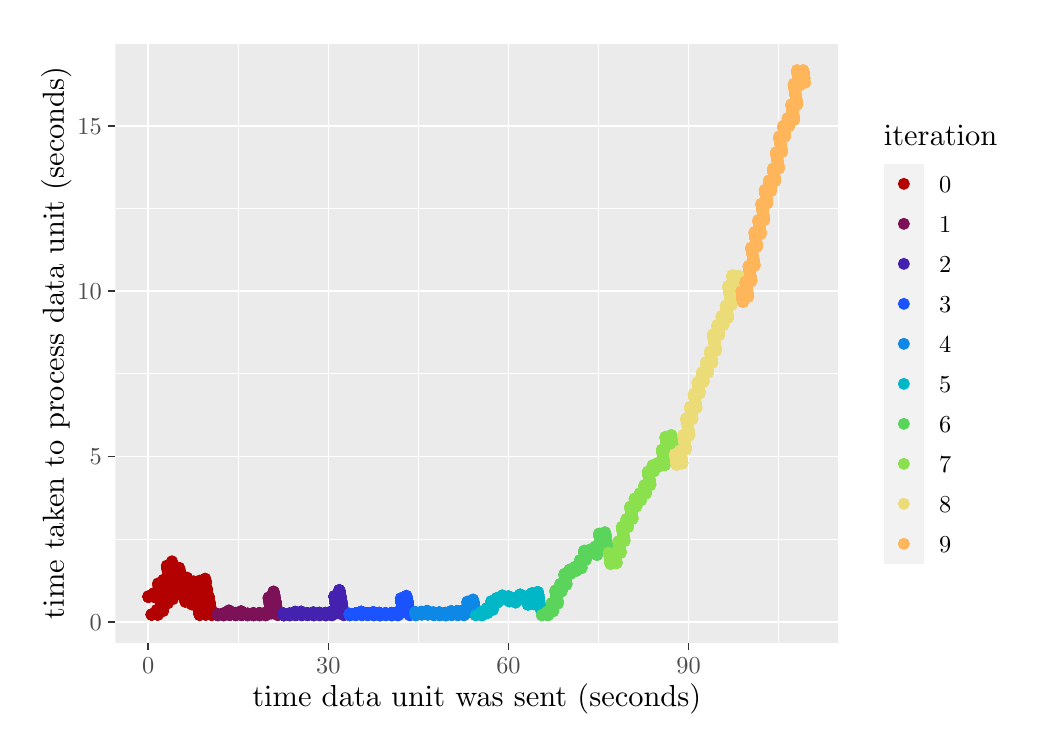
\begin{tikzpicture}[x=1pt,y=1pt]
	\definecolor{fillColor}{RGB}{255,255,255}
	\path[use as bounding box,fill=fillColor,fill opacity=0.00] (0,0) rectangle (361.35,252.94);
	\begin{scope}
	\path[clip] (  0.00,  0.00) rectangle (361.35,252.94);
	\definecolor{drawColor}{RGB}{255,255,255}
	\definecolor{fillColor}{RGB}{255,255,255}
	
	\path[draw=drawColor,line width= 0.6pt,line join=round,line cap=round,fill=fillColor] (  0.00,  0.00) rectangle (361.35,252.94);
	\end{scope}
	\begin{scope}
	\path[clip] ( 31.71, 30.69) rectangle (292.88,247.45);
	\definecolor{fillColor}{gray}{0.92}
	
	\path[fill=fillColor] ( 31.71, 30.69) rectangle (292.88,247.45);
	\definecolor{drawColor}{RGB}{255,255,255}
	
	\path[draw=drawColor,line width= 0.3pt,line join=round] ( 31.71, 68.14) --
		(292.88, 68.14);
	
	\path[draw=drawColor,line width= 0.3pt,line join=round] ( 31.71,127.85) --
		(292.88,127.85);
	
	\path[draw=drawColor,line width= 0.3pt,line join=round] ( 31.71,187.56) --
		(292.88,187.56);
	
	\path[draw=drawColor,line width= 0.3pt,line join=round] ( 31.71,247.28) --
		(292.88,247.28);
	
	\path[draw=drawColor,line width= 0.3pt,line join=round] ( 76.12, 30.69) --
		( 76.12,247.45);
	
	\path[draw=drawColor,line width= 0.3pt,line join=round] (141.19, 30.69) --
		(141.19,247.45);
	
	\path[draw=drawColor,line width= 0.3pt,line join=round] (206.26, 30.69) --
		(206.26,247.45);
	
	\path[draw=drawColor,line width= 0.3pt,line join=round] (271.32, 30.69) --
		(271.32,247.45);
	
	\path[draw=drawColor,line width= 0.6pt,line join=round] ( 31.71, 38.28) --
		(292.88, 38.28);
	
	\path[draw=drawColor,line width= 0.6pt,line join=round] ( 31.71, 97.99) --
		(292.88, 97.99);
	
	\path[draw=drawColor,line width= 0.6pt,line join=round] ( 31.71,157.71) --
		(292.88,157.71);
	
	\path[draw=drawColor,line width= 0.6pt,line join=round] ( 31.71,217.42) --
		(292.88,217.42);
	
	\path[draw=drawColor,line width= 0.6pt,line join=round] ( 43.58, 30.69) --
		( 43.58,247.45);
	
	\path[draw=drawColor,line width= 0.6pt,line join=round] (108.65, 30.69) --
		(108.65,247.45);
	
	\path[draw=drawColor,line width= 0.6pt,line join=round] (173.72, 30.69) --
		(173.72,247.45);
	
	\path[draw=drawColor,line width= 0.6pt,line join=round] (238.79, 30.69) --
		(238.79,247.45);
	\definecolor{drawColor}{RGB}{179,0,0}
	\definecolor{fillColor}{RGB}{179,0,0}
	
	\path[draw=drawColor,line width= 0.4pt,line join=round,line cap=round,fill=fillColor] ( 43.64, 47.23) circle (  1.96);
	
	\path[draw=drawColor,line width= 0.4pt,line join=round,line cap=round,fill=fillColor] ( 43.65, 47.14) circle (  1.96);
	
	\path[draw=drawColor,line width= 0.4pt,line join=round,line cap=round,fill=fillColor] ( 44.81, 40.75) circle (  1.96);
	
	\path[draw=drawColor,line width= 0.4pt,line join=round,line cap=round,fill=fillColor] ( 44.81, 40.79) circle (  1.96);
	
	\path[draw=drawColor,line width= 0.4pt,line join=round,line cap=round,fill=fillColor] ( 43.63, 47.29) circle (  1.96);
	
	\path[draw=drawColor,line width= 0.4pt,line join=round,line cap=round,fill=fillColor] ( 44.77, 40.99) circle (  1.96);
	
	\path[draw=drawColor,line width= 0.4pt,line join=round,line cap=round,fill=fillColor] ( 43.58, 47.52) circle (  1.96);
	
	\path[draw=drawColor,line width= 0.4pt,line join=round,line cap=round,fill=fillColor] ( 43.62, 47.32) circle (  1.96);
	
	\path[draw=drawColor,line width= 0.4pt,line join=round,line cap=round,fill=fillColor] ( 43.61, 47.38) circle (  1.96);
	
	\path[draw=drawColor,line width= 0.4pt,line join=round,line cap=round,fill=fillColor] ( 44.79, 40.90) circle (  1.96);
	
	\path[draw=drawColor,line width= 0.4pt,line join=round,line cap=round,fill=fillColor] ( 44.79, 40.86) circle (  1.96);
	
	\path[draw=drawColor,line width= 0.4pt,line join=round,line cap=round,fill=fillColor] ( 44.80, 40.85) circle (  1.96);
	
	\path[draw=drawColor,line width= 0.4pt,line join=round,line cap=round,fill=fillColor] ( 44.78, 40.93) circle (  1.96);
	
	\path[draw=drawColor,line width= 0.4pt,line join=round,line cap=round,fill=fillColor] ( 44.80, 40.80) circle (  1.96);
	
	\path[draw=drawColor,line width= 0.4pt,line join=round,line cap=round,fill=fillColor] ( 44.80, 40.83) circle (  1.96);
	
	\path[draw=drawColor,line width= 0.4pt,line join=round,line cap=round,fill=fillColor] ( 43.63, 47.25) circle (  1.96);
	
	\path[draw=drawColor,line width= 0.4pt,line join=round,line cap=round,fill=fillColor] ( 46.98, 40.79) circle (  1.96);
	
	\path[draw=drawColor,line width= 0.4pt,line join=round,line cap=round,fill=fillColor] ( 46.97, 40.83) circle (  1.96);
	
	\path[draw=drawColor,line width= 0.4pt,line join=round,line cap=round,fill=fillColor] ( 45.76, 47.50) circle (  1.96);
	
	\path[draw=drawColor,line width= 0.4pt,line join=round,line cap=round,fill=fillColor] ( 45.82, 47.17) circle (  1.96);
	
	\path[draw=drawColor,line width= 0.4pt,line join=round,line cap=round,fill=fillColor] ( 46.95, 40.94) circle (  1.96);
	
	\path[draw=drawColor,line width= 0.4pt,line join=round,line cap=round,fill=fillColor] ( 46.95, 40.93) circle (  1.96);
	
	\path[draw=drawColor,line width= 0.4pt,line join=round,line cap=round,fill=fillColor] ( 45.80, 47.26) circle (  1.96);
	
	\path[draw=drawColor,line width= 0.4pt,line join=round,line cap=round,fill=fillColor] ( 45.82, 47.15) circle (  1.96);
	
	\path[draw=drawColor,line width= 0.4pt,line join=round,line cap=round,fill=fillColor] ( 46.97, 40.81) circle (  1.96);
	
	\path[draw=drawColor,line width= 0.4pt,line join=round,line cap=round,fill=fillColor] ( 46.96, 40.90) circle (  1.96);
	
	\path[draw=drawColor,line width= 0.4pt,line join=round,line cap=round,fill=fillColor] ( 46.98, 40.78) circle (  1.96);
	
	\path[draw=drawColor,line width= 0.4pt,line join=round,line cap=round,fill=fillColor] ( 45.78, 47.36) circle (  1.96);
	
	\path[draw=drawColor,line width= 0.4pt,line join=round,line cap=round,fill=fillColor] ( 46.93, 41.06) circle (  1.96);
	
	\path[draw=drawColor,line width= 0.4pt,line join=round,line cap=round,fill=fillColor] ( 45.77, 47.45) circle (  1.96);
	
	\path[draw=drawColor,line width= 0.4pt,line join=round,line cap=round,fill=fillColor] ( 46.92, 41.08) circle (  1.96);
	
	\path[draw=drawColor,line width= 0.4pt,line join=round,line cap=round,fill=fillColor] ( 45.78, 47.38) circle (  1.96);
	
	\path[draw=drawColor,line width= 0.4pt,line join=round,line cap=round,fill=fillColor] ( 46.89, 41.27) circle (  1.96);
	
	\path[draw=drawColor,line width= 0.4pt,line join=round,line cap=round,fill=fillColor] ( 46.89, 41.26) circle (  1.96);
	
	\path[draw=drawColor,line width= 0.4pt,line join=round,line cap=round,fill=fillColor] ( 46.86, 41.45) circle (  1.96);
	
	\path[draw=drawColor,line width= 0.4pt,line join=round,line cap=round,fill=fillColor] ( 45.65, 48.11) circle (  1.96);
	
	\path[draw=drawColor,line width= 0.4pt,line join=round,line cap=round,fill=fillColor] ( 46.85, 41.48) circle (  1.96);
	
	\path[draw=drawColor,line width= 0.4pt,line join=round,line cap=round,fill=fillColor] ( 46.79, 41.80) circle (  1.96);
	
	\path[draw=drawColor,line width= 0.4pt,line join=round,line cap=round,fill=fillColor] ( 46.89, 41.28) circle (  1.96);
	
	\path[draw=drawColor,line width= 0.4pt,line join=round,line cap=round,fill=fillColor] ( 45.66, 48.01) circle (  1.96);
	
	\path[draw=drawColor,line width= 0.4pt,line join=round,line cap=round,fill=fillColor] ( 46.87, 41.39) circle (  1.96);
	
	\path[draw=drawColor,line width= 0.4pt,line join=round,line cap=round,fill=fillColor] ( 46.86, 41.43) circle (  1.96);
	
	\path[draw=drawColor,line width= 0.4pt,line join=round,line cap=round,fill=fillColor] ( 46.86, 41.42) circle (  1.96);
	
	\path[draw=drawColor,line width= 0.4pt,line join=round,line cap=round,fill=fillColor] ( 46.90, 41.21) circle (  1.96);
	
	\path[draw=drawColor,line width= 0.4pt,line join=round,line cap=round,fill=fillColor] ( 45.73, 47.63) circle (  1.96);
	
	\path[draw=drawColor,line width= 0.4pt,line join=round,line cap=round,fill=fillColor] ( 45.70, 47.84) circle (  1.96);
	
	\path[draw=drawColor,line width= 0.4pt,line join=round,line cap=round,fill=fillColor] ( 46.87, 41.36) circle (  1.96);
	
	\path[draw=drawColor,line width= 0.4pt,line join=round,line cap=round,fill=fillColor] ( 45.75, 47.55) circle (  1.96);
	
	\path[draw=drawColor,line width= 0.4pt,line join=round,line cap=round,fill=fillColor] ( 46.85, 41.49) circle (  1.96);
	
	\path[draw=drawColor,line width= 0.4pt,line join=round,line cap=round,fill=fillColor] ( 46.80, 41.73) circle (  1.96);
	
	\path[draw=drawColor,line width= 0.4pt,line join=round,line cap=round,fill=fillColor] ( 46.81, 41.71) circle (  1.96);
	
	\path[draw=drawColor,line width= 0.4pt,line join=round,line cap=round,fill=fillColor] ( 46.80, 41.76) circle (  1.96);
	
	\path[draw=drawColor,line width= 0.4pt,line join=round,line cap=round,fill=fillColor] ( 46.76, 41.96) circle (  1.96);
	
	\path[draw=drawColor,line width= 0.4pt,line join=round,line cap=round,fill=fillColor] ( 45.56, 48.56) circle (  1.96);
	
	\path[draw=drawColor,line width= 0.4pt,line join=round,line cap=round,fill=fillColor] ( 46.72, 42.22) circle (  1.96);
	
	\path[draw=drawColor,line width= 0.4pt,line join=round,line cap=round,fill=fillColor] ( 46.66, 42.52) circle (  1.96);
	
	\path[draw=drawColor,line width= 0.4pt,line join=round,line cap=round,fill=fillColor] ( 46.71, 42.26) circle (  1.96);
	
	\path[draw=drawColor,line width= 0.4pt,line join=round,line cap=round,fill=fillColor] ( 46.70, 42.28) circle (  1.96);
	
	\path[draw=drawColor,line width= 0.4pt,line join=round,line cap=round,fill=fillColor] ( 45.58, 48.46) circle (  1.96);
	
	\path[draw=drawColor,line width= 0.4pt,line join=round,line cap=round,fill=fillColor] ( 46.76, 41.98) circle (  1.96);
	
	\path[draw=drawColor,line width= 0.4pt,line join=round,line cap=round,fill=fillColor] ( 46.76, 42.00) circle (  1.96);
	
	\path[draw=drawColor,line width= 0.4pt,line join=round,line cap=round,fill=fillColor] ( 46.82, 41.65) circle (  1.96);
	
	\path[draw=drawColor,line width= 0.4pt,line join=round,line cap=round,fill=fillColor] ( 46.84, 41.52) circle (  1.96);
	
	\path[draw=drawColor,line width= 0.4pt,line join=round,line cap=round,fill=fillColor] ( 46.80, 41.78) circle (  1.96);
	
	\path[draw=drawColor,line width= 0.4pt,line join=round,line cap=round,fill=fillColor] ( 46.79, 41.79) circle (  1.96);
	
	\path[draw=drawColor,line width= 0.4pt,line join=round,line cap=round,fill=fillColor] ( 45.69, 47.90) circle (  1.96);
	
	\path[draw=drawColor,line width= 0.4pt,line join=round,line cap=round,fill=fillColor] ( 46.77, 41.95) circle (  1.96);
	
	\path[draw=drawColor,line width= 0.4pt,line join=round,line cap=round,fill=fillColor] ( 46.73, 42.13) circle (  1.96);
	
	\path[draw=drawColor,line width= 0.4pt,line join=round,line cap=round,fill=fillColor] ( 46.77, 41.91) circle (  1.96);
	
	\path[draw=drawColor,line width= 0.4pt,line join=round,line cap=round,fill=fillColor] ( 46.79, 41.83) circle (  1.96);
	
	\path[draw=drawColor,line width= 0.4pt,line join=round,line cap=round,fill=fillColor] ( 46.74, 42.09) circle (  1.96);
	
	\path[draw=drawColor,line width= 0.4pt,line join=round,line cap=round,fill=fillColor] ( 46.74, 42.11) circle (  1.96);
	
	\path[draw=drawColor,line width= 0.4pt,line join=round,line cap=round,fill=fillColor] ( 45.61, 48.29) circle (  1.96);
	
	\path[draw=drawColor,line width= 0.4pt,line join=round,line cap=round,fill=fillColor] ( 46.78, 41.86) circle (  1.96);
	
	\path[draw=drawColor,line width= 0.4pt,line join=round,line cap=round,fill=fillColor] ( 46.77, 41.94) circle (  1.96);
	
	\path[draw=drawColor,line width= 0.4pt,line join=round,line cap=round,fill=fillColor] ( 46.72, 42.17) circle (  1.96);
	
	\path[draw=drawColor,line width= 0.4pt,line join=round,line cap=round,fill=fillColor] ( 45.57, 48.55) circle (  1.96);
	
	\path[draw=drawColor,line width= 0.4pt,line join=round,line cap=round,fill=fillColor] ( 46.75, 42.04) circle (  1.96);
	
	\path[draw=drawColor,line width= 0.4pt,line join=round,line cap=round,fill=fillColor] ( 46.77, 41.90) circle (  1.96);
	
	\path[draw=drawColor,line width= 0.4pt,line join=round,line cap=round,fill=fillColor] ( 46.78, 41.88) circle (  1.96);
	
	\path[draw=drawColor,line width= 0.4pt,line join=round,line cap=round,fill=fillColor] ( 46.73, 42.15) circle (  1.96);
	
	\path[draw=drawColor,line width= 0.4pt,line join=round,line cap=round,fill=fillColor] ( 46.75, 42.01) circle (  1.96);
	
	\path[draw=drawColor,line width= 0.4pt,line join=round,line cap=round,fill=fillColor] ( 46.81, 41.72) circle (  1.96);
	
	\path[draw=drawColor,line width= 0.4pt,line join=round,line cap=round,fill=fillColor] ( 46.77, 41.92) circle (  1.96);
	
	\path[draw=drawColor,line width= 0.4pt,line join=round,line cap=round,fill=fillColor] ( 46.70, 42.33) circle (  1.96);
	
	\path[draw=drawColor,line width= 0.4pt,line join=round,line cap=round,fill=fillColor] ( 46.66, 42.54) circle (  1.96);
	
	\path[draw=drawColor,line width= 0.4pt,line join=round,line cap=round,fill=fillColor] ( 46.73, 42.16) circle (  1.96);
	
	\path[draw=drawColor,line width= 0.4pt,line join=round,line cap=round,fill=fillColor] ( 45.59, 48.41) circle (  1.96);
	
	\path[draw=drawColor,line width= 0.4pt,line join=round,line cap=round,fill=fillColor] ( 48.87, 42.28) circle (  1.96);
	
	\path[draw=drawColor,line width= 0.4pt,line join=round,line cap=round,fill=fillColor] ( 48.86, 42.34) circle (  1.96);
	
	\path[draw=drawColor,line width= 0.4pt,line join=round,line cap=round,fill=fillColor] ( 47.72, 48.66) circle (  1.96);
	
	\path[draw=drawColor,line width= 0.4pt,line join=round,line cap=round,fill=fillColor] ( 47.65, 48.99) circle (  1.96);
	
	\path[draw=drawColor,line width= 0.4pt,line join=round,line cap=round,fill=fillColor] ( 47.67, 48.91) circle (  1.96);
	
	\path[draw=drawColor,line width= 0.4pt,line join=round,line cap=round,fill=fillColor] ( 47.68, 48.84) circle (  1.96);
	
	\path[draw=drawColor,line width= 0.4pt,line join=round,line cap=round,fill=fillColor] ( 48.87, 42.33) circle (  1.96);
	
	\path[draw=drawColor,line width= 0.4pt,line join=round,line cap=round,fill=fillColor] ( 48.84, 42.46) circle (  1.96);
	
	\path[draw=drawColor,line width= 0.4pt,line join=round,line cap=round,fill=fillColor] ( 48.86, 42.38) circle (  1.96);
	
	\path[draw=drawColor,line width= 0.4pt,line join=round,line cap=round,fill=fillColor] ( 48.89, 42.19) circle (  1.96);
	
	\path[draw=drawColor,line width= 0.4pt,line join=round,line cap=round,fill=fillColor] ( 47.72, 48.62) circle (  1.96);
	
	\path[draw=drawColor,line width= 0.4pt,line join=round,line cap=round,fill=fillColor] ( 48.86, 42.35) circle (  1.96);
	
	\path[draw=drawColor,line width= 0.4pt,line join=round,line cap=round,fill=fillColor] ( 48.82, 42.59) circle (  1.96);
	
	\path[draw=drawColor,line width= 0.4pt,line join=round,line cap=round,fill=fillColor] ( 48.82, 42.56) circle (  1.96);
	
	\path[draw=drawColor,line width= 0.4pt,line join=round,line cap=round,fill=fillColor] ( 48.77, 42.84) circle (  1.96);
	
	\path[draw=drawColor,line width= 0.4pt,line join=round,line cap=round,fill=fillColor] ( 48.80, 42.68) circle (  1.96);
	
	\path[draw=drawColor,line width= 0.4pt,line join=round,line cap=round,fill=fillColor] ( 47.63, 49.15) circle (  1.96);
	
	\path[draw=drawColor,line width= 0.4pt,line join=round,line cap=round,fill=fillColor] ( 48.84, 42.49) circle (  1.96);
	
	\path[draw=drawColor,line width= 0.4pt,line join=round,line cap=round,fill=fillColor] ( 48.81, 42.62) circle (  1.96);
	
	\path[draw=drawColor,line width= 0.4pt,line join=round,line cap=round,fill=fillColor] ( 48.78, 42.77) circle (  1.96);
	
	\path[draw=drawColor,line width= 0.4pt,line join=round,line cap=round,fill=fillColor] ( 48.81, 42.63) circle (  1.96);
	
	\path[draw=drawColor,line width= 0.4pt,line join=round,line cap=round,fill=fillColor] ( 48.80, 42.70) circle (  1.96);
	
	\path[draw=drawColor,line width= 0.4pt,line join=round,line cap=round,fill=fillColor] ( 48.81, 42.64) circle (  1.96);
	
	\path[draw=drawColor,line width= 0.4pt,line join=round,line cap=round,fill=fillColor] ( 48.88, 42.27) circle (  1.96);
	
	\path[draw=drawColor,line width= 0.4pt,line join=round,line cap=round,fill=fillColor] ( 47.78, 48.28) circle (  1.96);
	
	\path[draw=drawColor,line width= 0.4pt,line join=round,line cap=round,fill=fillColor] ( 48.90, 42.11) circle (  1.96);
	
	\path[draw=drawColor,line width= 0.4pt,line join=round,line cap=round,fill=fillColor] ( 47.75, 48.49) circle (  1.96);
	
	\path[draw=drawColor,line width= 0.4pt,line join=round,line cap=round,fill=fillColor] ( 48.85, 42.41) circle (  1.96);
	
	\path[draw=drawColor,line width= 0.4pt,line join=round,line cap=round,fill=fillColor] ( 48.77, 42.87) circle (  1.96);
	
	\path[draw=drawColor,line width= 0.4pt,line join=round,line cap=round,fill=fillColor] ( 48.83, 42.54) circle (  1.96);
	
	\path[draw=drawColor,line width= 0.4pt,line join=round,line cap=round,fill=fillColor] ( 47.59, 49.38) circle (  1.96);
	
	\path[draw=drawColor,line width= 0.4pt,line join=round,line cap=round,fill=fillColor] ( 48.66, 43.45) circle (  1.96);
	
	\path[draw=drawColor,line width= 0.4pt,line join=round,line cap=round,fill=fillColor] ( 47.47, 50.03) circle (  1.96);
	
	\path[draw=drawColor,line width= 0.4pt,line join=round,line cap=round,fill=fillColor] ( 48.64, 43.57) circle (  1.96);
	
	\path[draw=drawColor,line width= 0.4pt,line join=round,line cap=round,fill=fillColor] ( 47.44, 50.20) circle (  1.96);
	
	\path[draw=drawColor,line width= 0.4pt,line join=round,line cap=round,fill=fillColor] ( 48.55, 44.09) circle (  1.96);
	
	\path[draw=drawColor,line width= 0.4pt,line join=round,line cap=round,fill=fillColor] ( 47.45, 50.10) circle (  1.96);
	
	\path[draw=drawColor,line width= 0.4pt,line join=round,line cap=round,fill=fillColor] ( 48.53, 44.17) circle (  1.96);
	
	\path[draw=drawColor,line width= 0.4pt,line join=round,line cap=round,fill=fillColor] ( 47.43, 50.24) circle (  1.96);
	
	\path[draw=drawColor,line width= 0.4pt,line join=round,line cap=round,fill=fillColor] ( 48.52, 44.25) circle (  1.96);
	
	\path[draw=drawColor,line width= 0.4pt,line join=round,line cap=round,fill=fillColor] ( 48.55, 44.07) circle (  1.96);
	
	\path[draw=drawColor,line width= 0.4pt,line join=round,line cap=round,fill=fillColor] ( 48.54, 44.11) circle (  1.96);
	
	\path[draw=drawColor,line width= 0.4pt,line join=round,line cap=round,fill=fillColor] ( 48.63, 43.64) circle (  1.96);
	
	\path[draw=drawColor,line width= 0.4pt,line join=round,line cap=round,fill=fillColor] ( 47.53, 49.66) circle (  1.96);
	
	\path[draw=drawColor,line width= 0.4pt,line join=round,line cap=round,fill=fillColor] ( 48.66, 43.46) circle (  1.96);
	
	\path[draw=drawColor,line width= 0.4pt,line join=round,line cap=round,fill=fillColor] ( 48.62, 43.70) circle (  1.96);
	
	\path[draw=drawColor,line width= 0.4pt,line join=round,line cap=round,fill=fillColor] ( 47.38, 50.52) circle (  1.96);
	
	\path[draw=drawColor,line width= 0.4pt,line join=round,line cap=round,fill=fillColor] ( 48.62, 43.67) circle (  1.96);
	
	\path[draw=drawColor,line width= 0.4pt,line join=round,line cap=round,fill=fillColor] ( 48.57, 43.94) circle (  1.96);
	
	\path[draw=drawColor,line width= 0.4pt,line join=round,line cap=round,fill=fillColor] ( 47.37, 50.58) circle (  1.96);
	
	\path[draw=drawColor,line width= 0.4pt,line join=round,line cap=round,fill=fillColor] ( 48.58, 43.92) circle (  1.96);
	
	\path[draw=drawColor,line width= 0.4pt,line join=round,line cap=round,fill=fillColor] ( 48.50, 44.32) circle (  1.96);
	
	\path[draw=drawColor,line width= 0.4pt,line join=round,line cap=round,fill=fillColor] ( 48.56, 44.03) circle (  1.96);
	
	\path[draw=drawColor,line width= 0.4pt,line join=round,line cap=round,fill=fillColor] ( 48.54, 44.12) circle (  1.96);
	
	\path[draw=drawColor,line width= 0.4pt,line join=round,line cap=round,fill=fillColor] ( 48.49, 44.42) circle (  1.96);
	
	\path[draw=drawColor,line width= 0.4pt,line join=round,line cap=round,fill=fillColor] ( 48.46, 44.58) circle (  1.96);
	
	\path[draw=drawColor,line width= 0.4pt,line join=round,line cap=round,fill=fillColor] ( 48.44, 44.67) circle (  1.96);
	
	\path[draw=drawColor,line width= 0.4pt,line join=round,line cap=round,fill=fillColor] ( 48.47, 44.48) circle (  1.96);
	
	\path[draw=drawColor,line width= 0.4pt,line join=round,line cap=round,fill=fillColor] ( 48.41, 44.83) circle (  1.96);
	
	\path[draw=drawColor,line width= 0.4pt,line join=round,line cap=round,fill=fillColor] ( 48.42, 44.78) circle (  1.96);
	
	\path[draw=drawColor,line width= 0.4pt,line join=round,line cap=round,fill=fillColor] ( 48.42, 44.79) circle (  1.96);
	
	\path[draw=drawColor,line width= 0.4pt,line join=round,line cap=round,fill=fillColor] ( 48.37, 45.06) circle (  1.96);
	
	\path[draw=drawColor,line width= 0.4pt,line join=round,line cap=round,fill=fillColor] ( 48.34, 45.21) circle (  1.96);
	
	\path[draw=drawColor,line width= 0.4pt,line join=round,line cap=round,fill=fillColor] ( 47.09, 52.12) circle (  1.96);
	
	\path[draw=drawColor,line width= 0.4pt,line join=round,line cap=round,fill=fillColor] ( 48.37, 45.03) circle (  1.96);
	
	\path[draw=drawColor,line width= 0.4pt,line join=round,line cap=round,fill=fillColor] ( 47.23, 51.33) circle (  1.96);
	
	\path[draw=drawColor,line width= 0.4pt,line join=round,line cap=round,fill=fillColor] ( 48.21, 45.92) circle (  1.96);
	
	\path[draw=drawColor,line width= 0.4pt,line join=round,line cap=round,fill=fillColor] ( 48.27, 45.59) circle (  1.96);
	
	\path[draw=drawColor,line width= 0.4pt,line join=round,line cap=round,fill=fillColor] ( 48.28, 45.57) circle (  1.96);
	
	\path[draw=drawColor,line width= 0.4pt,line join=round,line cap=round,fill=fillColor] ( 48.32, 45.33) circle (  1.96);
	
	\path[draw=drawColor,line width= 0.4pt,line join=round,line cap=round,fill=fillColor] ( 48.39, 44.97) circle (  1.96);
	
	\path[draw=drawColor,line width= 0.4pt,line join=round,line cap=round,fill=fillColor] ( 47.25, 51.23) circle (  1.96);
	
	\path[draw=drawColor,line width= 0.4pt,line join=round,line cap=round,fill=fillColor] ( 47.18, 51.61) circle (  1.96);
	
	\path[draw=drawColor,line width= 0.4pt,line join=round,line cap=round,fill=fillColor] ( 48.40, 44.91) circle (  1.96);
	
	\path[draw=drawColor,line width= 0.4pt,line join=round,line cap=round,fill=fillColor] ( 48.30, 45.46) circle (  1.96);
	
	\path[draw=drawColor,line width= 0.4pt,line join=round,line cap=round,fill=fillColor] ( 48.28, 45.53) circle (  1.96);
	
	\path[draw=drawColor,line width= 0.4pt,line join=round,line cap=round,fill=fillColor] ( 48.30, 45.45) circle (  1.96);
	
	\path[draw=drawColor,line width= 0.4pt,line join=round,line cap=round,fill=fillColor] ( 50.45, 45.52) circle (  1.96);
	
	\path[draw=drawColor,line width= 0.4pt,line join=round,line cap=round,fill=fillColor] ( 50.44, 45.59) circle (  1.96);
	
	\path[draw=drawColor,line width= 0.4pt,line join=round,line cap=round,fill=fillColor] ( 49.34, 51.66) circle (  1.96);
	
	\path[draw=drawColor,line width= 0.4pt,line join=round,line cap=round,fill=fillColor] ( 49.38, 51.43) circle (  1.96);
	
	\path[draw=drawColor,line width= 0.4pt,line join=round,line cap=round,fill=fillColor] ( 50.47, 45.43) circle (  1.96);
	
	\path[draw=drawColor,line width= 0.4pt,line join=round,line cap=round,fill=fillColor] ( 50.49, 45.30) circle (  1.96);
	
	\path[draw=drawColor,line width= 0.4pt,line join=round,line cap=round,fill=fillColor] ( 50.47, 45.41) circle (  1.96);
	
	\path[draw=drawColor,line width= 0.4pt,line join=round,line cap=round,fill=fillColor] ( 50.55, 45.01) circle (  1.96);
	
	\path[draw=drawColor,line width= 0.4pt,line join=round,line cap=round,fill=fillColor] ( 49.37, 51.51) circle (  1.96);
	
	\path[draw=drawColor,line width= 0.4pt,line join=round,line cap=round,fill=fillColor] ( 50.52, 45.17) circle (  1.96);
	
	\path[draw=drawColor,line width= 0.4pt,line join=round,line cap=round,fill=fillColor] ( 50.40, 45.81) circle (  1.96);
	
	\path[draw=drawColor,line width= 0.4pt,line join=round,line cap=round,fill=fillColor] ( 50.30, 46.35) circle (  1.96);
	
	\path[draw=drawColor,line width= 0.4pt,line join=round,line cap=round,fill=fillColor] ( 50.29, 46.43) circle (  1.96);
	
	\path[draw=drawColor,line width= 0.4pt,line join=round,line cap=round,fill=fillColor] ( 50.37, 45.98) circle (  1.96);
	
	\path[draw=drawColor,line width= 0.4pt,line join=round,line cap=round,fill=fillColor] ( 50.28, 46.46) circle (  1.96);
	
	\path[draw=drawColor,line width= 0.4pt,line join=round,line cap=round,fill=fillColor] ( 50.31, 46.32) circle (  1.96);
	
	\path[draw=drawColor,line width= 0.4pt,line join=round,line cap=round,fill=fillColor] ( 50.29, 46.44) circle (  1.96);
	
	\path[draw=drawColor,line width= 0.4pt,line join=round,line cap=round,fill=fillColor] ( 50.29, 46.41) circle (  1.96);
	
	\path[draw=drawColor,line width= 0.4pt,line join=round,line cap=round,fill=fillColor] ( 50.26, 46.57) circle (  1.96);
	
	\path[draw=drawColor,line width= 0.4pt,line join=round,line cap=round,fill=fillColor] ( 50.29, 46.40) circle (  1.96);
	
	\path[draw=drawColor,line width= 0.4pt,line join=round,line cap=round,fill=fillColor] ( 50.32, 46.27) circle (  1.96);
	
	\path[draw=drawColor,line width= 0.4pt,line join=round,line cap=round,fill=fillColor] ( 50.34, 46.18) circle (  1.96);
	
	\path[draw=drawColor,line width= 0.4pt,line join=round,line cap=round,fill=fillColor] ( 50.30, 46.37) circle (  1.96);
	
	\path[draw=drawColor,line width= 0.4pt,line join=round,line cap=round,fill=fillColor] ( 50.31, 46.29) circle (  1.96);
	
	\path[draw=drawColor,line width= 0.4pt,line join=round,line cap=round,fill=fillColor] ( 50.31, 46.31) circle (  1.96);
	
	\path[draw=drawColor,line width= 0.4pt,line join=round,line cap=round,fill=fillColor] ( 50.38, 45.91) circle (  1.96);
	
	\path[draw=drawColor,line width= 0.4pt,line join=round,line cap=round,fill=fillColor] ( 50.33, 46.21) circle (  1.96);
	
	\path[draw=drawColor,line width= 0.4pt,line join=round,line cap=round,fill=fillColor] ( 50.39, 45.90) circle (  1.96);
	
	\path[draw=drawColor,line width= 0.4pt,line join=round,line cap=round,fill=fillColor] ( 50.38, 45.92) circle (  1.96);
	
	\path[draw=drawColor,line width= 0.4pt,line join=round,line cap=round,fill=fillColor] ( 50.45, 45.57) circle (  1.96);
	
	\path[draw=drawColor,line width= 0.4pt,line join=round,line cap=round,fill=fillColor] ( 50.46, 45.47) circle (  1.96);
	
	\path[draw=drawColor,line width= 0.4pt,line join=round,line cap=round,fill=fillColor] ( 50.50, 45.26) circle (  1.96);
	
	\path[draw=drawColor,line width= 0.4pt,line join=round,line cap=round,fill=fillColor] ( 50.44, 45.58) circle (  1.96);
	
	\path[draw=drawColor,line width= 0.4pt,line join=round,line cap=round,fill=fillColor] ( 50.27, 46.55) circle (  1.96);
	
	\path[draw=drawColor,line width= 0.4pt,line join=round,line cap=round,fill=fillColor] ( 50.41, 45.76) circle (  1.96);
	
	\path[draw=drawColor,line width= 0.4pt,line join=round,line cap=round,fill=fillColor] ( 50.32, 46.25) circle (  1.96);
	
	\path[draw=drawColor,line width= 0.4pt,line join=round,line cap=round,fill=fillColor] ( 49.12, 52.88) circle (  1.96);
	
	\path[draw=drawColor,line width= 0.4pt,line join=round,line cap=round,fill=fillColor] ( 50.28, 46.49) circle (  1.96);
	
	\path[draw=drawColor,line width= 0.4pt,line join=round,line cap=round,fill=fillColor] ( 49.11, 52.95) circle (  1.96);
	
	\path[draw=drawColor,line width= 0.4pt,line join=round,line cap=round,fill=fillColor] ( 49.12, 52.86) circle (  1.96);
	
	\path[draw=drawColor,line width= 0.4pt,line join=round,line cap=round,fill=fillColor] ( 50.27, 46.51) circle (  1.96);
	
	\path[draw=drawColor,line width= 0.4pt,line join=round,line cap=round,fill=fillColor] ( 50.29, 46.45) circle (  1.96);
	
	\path[draw=drawColor,line width= 0.4pt,line join=round,line cap=round,fill=fillColor] ( 50.41, 45.79) circle (  1.96);
	
	\path[draw=drawColor,line width= 0.4pt,line join=round,line cap=round,fill=fillColor] ( 49.14, 52.77) circle (  1.96);
	
	\path[draw=drawColor,line width= 0.4pt,line join=round,line cap=round,fill=fillColor] ( 50.41, 45.78) circle (  1.96);
	
	\path[draw=drawColor,line width= 0.4pt,line join=round,line cap=round,fill=fillColor] ( 50.32, 46.28) circle (  1.96);
	
	\path[draw=drawColor,line width= 0.4pt,line join=round,line cap=round,fill=fillColor] ( 50.43, 45.64) circle (  1.96);
	
	\path[draw=drawColor,line width= 0.4pt,line join=round,line cap=round,fill=fillColor] ( 50.56, 44.96) circle (  1.96);
	
	\path[draw=drawColor,line width= 0.4pt,line join=round,line cap=round,fill=fillColor] ( 50.56, 44.93) circle (  1.96);
	
	\path[draw=drawColor,line width= 0.4pt,line join=round,line cap=round,fill=fillColor] ( 49.32, 51.78) circle (  1.96);
	
	\path[draw=drawColor,line width= 0.4pt,line join=round,line cap=round,fill=fillColor] ( 49.26, 52.12) circle (  1.96);
	
	\path[draw=drawColor,line width= 0.4pt,line join=round,line cap=round,fill=fillColor] ( 50.46, 45.49) circle (  1.96);
	
	\path[draw=drawColor,line width= 0.4pt,line join=round,line cap=round,fill=fillColor] ( 50.45, 45.53) circle (  1.96);
	
	\path[draw=drawColor,line width= 0.4pt,line join=round,line cap=round,fill=fillColor] ( 50.40, 45.83) circle (  1.96);
	
	\path[draw=drawColor,line width= 0.4pt,line join=round,line cap=round,fill=fillColor] ( 49.29, 51.92) circle (  1.96);
	
	\path[draw=drawColor,line width= 0.4pt,line join=round,line cap=round,fill=fillColor] ( 49.24, 52.21) circle (  1.96);
	
	\path[draw=drawColor,line width= 0.4pt,line join=round,line cap=round,fill=fillColor] ( 50.42, 45.69) circle (  1.96);
	
	\path[draw=drawColor,line width= 0.4pt,line join=round,line cap=round,fill=fillColor] ( 50.42, 45.71) circle (  1.96);
	
	\path[draw=drawColor,line width= 0.4pt,line join=round,line cap=round,fill=fillColor] ( 50.48, 45.38) circle (  1.96);
	
	\path[draw=drawColor,line width= 0.4pt,line join=round,line cap=round,fill=fillColor] ( 49.33, 51.70) circle (  1.96);
	
	\path[draw=drawColor,line width= 0.4pt,line join=round,line cap=round,fill=fillColor] ( 50.53, 45.11) circle (  1.96);
	
	\path[draw=drawColor,line width= 0.4pt,line join=round,line cap=round,fill=fillColor] ( 49.32, 51.76) circle (  1.96);
	
	\path[draw=drawColor,line width= 0.4pt,line join=round,line cap=round,fill=fillColor] ( 50.42, 45.73) circle (  1.96);
	
	\path[draw=drawColor,line width= 0.4pt,line join=round,line cap=round,fill=fillColor] ( 50.35, 46.08) circle (  1.96);
	
	\path[draw=drawColor,line width= 0.4pt,line join=round,line cap=round,fill=fillColor] ( 50.33, 46.22) circle (  1.96);
	
	\path[draw=drawColor,line width= 0.4pt,line join=round,line cap=round,fill=fillColor] ( 50.46, 45.51) circle (  1.96);
	
	\path[draw=drawColor,line width= 0.4pt,line join=round,line cap=round,fill=fillColor] ( 50.45, 45.54) circle (  1.96);
	
	\path[draw=drawColor,line width= 0.4pt,line join=round,line cap=round,fill=fillColor] ( 50.47, 45.46) circle (  1.96);
	
	\path[draw=drawColor,line width= 0.4pt,line join=round,line cap=round,fill=fillColor] ( 49.31, 51.80) circle (  1.96);
	
	\path[draw=drawColor,line width= 0.4pt,line join=round,line cap=round,fill=fillColor] ( 50.55, 45.02) circle (  1.96);
	
	\path[draw=drawColor,line width= 0.4pt,line join=round,line cap=round,fill=fillColor] ( 50.55, 44.98) circle (  1.96);
	
	\path[draw=drawColor,line width= 0.4pt,line join=round,line cap=round,fill=fillColor] ( 49.30, 51.87) circle (  1.96);
	
	\path[draw=drawColor,line width= 0.4pt,line join=round,line cap=round,fill=fillColor] ( 49.41, 51.27) circle (  1.96);
	
	\path[draw=drawColor,line width= 0.4pt,line join=round,line cap=round,fill=fillColor] ( 49.37, 51.48) circle (  1.96);
	
	\path[draw=drawColor,line width= 0.4pt,line join=round,line cap=round,fill=fillColor] ( 50.50, 45.28) circle (  1.96);
	
	\path[draw=drawColor,line width= 0.4pt,line join=round,line cap=round,fill=fillColor] ( 50.47, 45.45) circle (  1.96);
	
	\path[draw=drawColor,line width= 0.4pt,line join=round,line cap=round,fill=fillColor] ( 50.47, 45.42) circle (  1.96);
	
	\path[draw=drawColor,line width= 0.4pt,line join=round,line cap=round,fill=fillColor] ( 50.24, 46.69) circle (  1.96);
	
	\path[draw=drawColor,line width= 0.4pt,line join=round,line cap=round,fill=fillColor] ( 49.01, 53.46) circle (  1.96);
	
	\path[draw=drawColor,line width= 0.4pt,line join=round,line cap=round,fill=fillColor] ( 50.32, 46.24) circle (  1.96);
	
	\path[draw=drawColor,line width= 0.4pt,line join=round,line cap=round,fill=fillColor] ( 52.34, 47.06) circle (  1.96);
	
	\path[draw=drawColor,line width= 0.4pt,line join=round,line cap=round,fill=fillColor] ( 52.46, 46.41) circle (  1.96);
	
	\path[draw=drawColor,line width= 0.4pt,line join=round,line cap=round,fill=fillColor] ( 52.39, 46.82) circle (  1.96);
	
	\path[draw=drawColor,line width= 0.4pt,line join=round,line cap=round,fill=fillColor] ( 51.07, 54.09) circle (  1.96);
	
	\path[draw=drawColor,line width= 0.4pt,line join=round,line cap=round,fill=fillColor] ( 52.32, 47.18) circle (  1.96);
	
	\path[draw=drawColor,line width= 0.4pt,line join=round,line cap=round,fill=fillColor] ( 52.24, 47.66) circle (  1.96);
	
	\path[draw=drawColor,line width= 0.4pt,line join=round,line cap=round,fill=fillColor] ( 52.28, 47.43) circle (  1.96);
	
	\path[draw=drawColor,line width= 0.4pt,line join=round,line cap=round,fill=fillColor] ( 52.31, 47.24) circle (  1.96);
	
	\path[draw=drawColor,line width= 0.4pt,line join=round,line cap=round,fill=fillColor] ( 51.18, 53.47) circle (  1.96);
	
	\path[draw=drawColor,line width= 0.4pt,line join=round,line cap=round,fill=fillColor] ( 51.14, 53.69) circle (  1.96);
	
	\path[draw=drawColor,line width= 0.4pt,line join=round,line cap=round,fill=fillColor] ( 52.30, 47.29) circle (  1.96);
	
	\path[draw=drawColor,line width= 0.4pt,line join=round,line cap=round,fill=fillColor] ( 52.16, 48.05) circle (  1.96);
	
	\path[draw=drawColor,line width= 0.4pt,line join=round,line cap=round,fill=fillColor] ( 52.12, 48.30) circle (  1.96);
	
	\path[draw=drawColor,line width= 0.4pt,line join=round,line cap=round,fill=fillColor] ( 52.09, 48.44) circle (  1.96);
	
	\path[draw=drawColor,line width= 0.4pt,line join=round,line cap=round,fill=fillColor] ( 51.97, 49.10) circle (  1.96);
	
	\path[draw=drawColor,line width= 0.4pt,line join=round,line cap=round,fill=fillColor] ( 51.99, 49.03) circle (  1.96);
	
	\path[draw=drawColor,line width= 0.4pt,line join=round,line cap=round,fill=fillColor] ( 51.98, 49.04) circle (  1.96);
	
	\path[draw=drawColor,line width= 0.4pt,line join=round,line cap=round,fill=fillColor] ( 51.99, 49.02) circle (  1.96);
	
	\path[draw=drawColor,line width= 0.4pt,line join=round,line cap=round,fill=fillColor] ( 51.77, 50.24) circle (  1.96);
	
	\path[draw=drawColor,line width= 0.4pt,line join=round,line cap=round,fill=fillColor] ( 50.73, 55.93) circle (  1.96);
	
	\path[draw=drawColor,line width= 0.4pt,line join=round,line cap=round,fill=fillColor] ( 51.87, 49.67) circle (  1.96);
	
	\path[draw=drawColor,line width= 0.4pt,line join=round,line cap=round,fill=fillColor] ( 50.64, 56.46) circle (  1.96);
	
	\path[draw=drawColor,line width= 0.4pt,line join=round,line cap=round,fill=fillColor] ( 51.93, 49.35) circle (  1.96);
	
	\path[draw=drawColor,line width= 0.4pt,line join=round,line cap=round,fill=fillColor] ( 51.80, 50.04) circle (  1.96);
	
	\path[draw=drawColor,line width= 0.4pt,line join=round,line cap=round,fill=fillColor] ( 51.79, 50.10) circle (  1.96);
	
	\path[draw=drawColor,line width= 0.4pt,line join=round,line cap=round,fill=fillColor] ( 50.63, 56.48) circle (  1.96);
	
	\path[draw=drawColor,line width= 0.4pt,line join=round,line cap=round,fill=fillColor] ( 51.80, 50.03) circle (  1.96);
	
	\path[draw=drawColor,line width= 0.4pt,line join=round,line cap=round,fill=fillColor] ( 51.88, 49.64) circle (  1.96);
	
	\path[draw=drawColor,line width= 0.4pt,line join=round,line cap=round,fill=fillColor] ( 51.87, 49.65) circle (  1.96);
	
	\path[draw=drawColor,line width= 0.4pt,line join=round,line cap=round,fill=fillColor] ( 51.70, 50.58) circle (  1.96);
	
	\path[draw=drawColor,line width= 0.4pt,line join=round,line cap=round,fill=fillColor] ( 51.70, 50.63) circle (  1.96);
	
	\path[draw=drawColor,line width= 0.4pt,line join=round,line cap=round,fill=fillColor] ( 50.51, 57.14) circle (  1.96);
	
	\path[draw=drawColor,line width= 0.4pt,line join=round,line cap=round,fill=fillColor] ( 51.66, 50.81) circle (  1.96);
	
	\path[draw=drawColor,line width= 0.4pt,line join=round,line cap=round,fill=fillColor] ( 51.54, 51.48) circle (  1.96);
	
	\path[draw=drawColor,line width= 0.4pt,line join=round,line cap=round,fill=fillColor] ( 51.56, 51.38) circle (  1.96);
	
	\path[draw=drawColor,line width= 0.4pt,line join=round,line cap=round,fill=fillColor] ( 51.58, 51.29) circle (  1.96);
	
	\path[draw=drawColor,line width= 0.4pt,line join=round,line cap=round,fill=fillColor] ( 50.42, 57.66) circle (  1.96);
	
	\path[draw=drawColor,line width= 0.4pt,line join=round,line cap=round,fill=fillColor] ( 50.39, 57.80) circle (  1.96);
	
	\path[draw=drawColor,line width= 0.4pt,line join=round,line cap=round,fill=fillColor] ( 51.65, 50.89) circle (  1.96);
	
	\path[draw=drawColor,line width= 0.4pt,line join=round,line cap=round,fill=fillColor] ( 51.64, 50.92) circle (  1.96);
	
	\path[draw=drawColor,line width= 0.4pt,line join=round,line cap=round,fill=fillColor] ( 50.45, 57.47) circle (  1.96);
	
	\path[draw=drawColor,line width= 0.4pt,line join=round,line cap=round,fill=fillColor] ( 51.61, 51.10) circle (  1.96);
	
	\path[draw=drawColor,line width= 0.4pt,line join=round,line cap=round,fill=fillColor] ( 51.74, 50.38) circle (  1.96);
	
	\path[draw=drawColor,line width= 0.4pt,line join=round,line cap=round,fill=fillColor] ( 51.88, 49.60) circle (  1.96);
	
	\path[draw=drawColor,line width= 0.4pt,line join=round,line cap=round,fill=fillColor] ( 51.66, 50.82) circle (  1.96);
	
	\path[draw=drawColor,line width= 0.4pt,line join=round,line cap=round,fill=fillColor] ( 51.70, 50.62) circle (  1.96);
	
	\path[draw=drawColor,line width= 0.4pt,line join=round,line cap=round,fill=fillColor] ( 51.69, 50.64) circle (  1.96);
	
	\path[draw=drawColor,line width= 0.4pt,line join=round,line cap=round,fill=fillColor] ( 51.71, 50.56) circle (  1.96);
	
	\path[draw=drawColor,line width= 0.4pt,line join=round,line cap=round,fill=fillColor] ( 51.86, 49.71) circle (  1.96);
	
	\path[draw=drawColor,line width= 0.4pt,line join=round,line cap=round,fill=fillColor] ( 51.73, 50.44) circle (  1.96);
	
	\path[draw=drawColor,line width= 0.4pt,line join=round,line cap=round,fill=fillColor] ( 51.76, 50.26) circle (  1.96);
	
	\path[draw=drawColor,line width= 0.4pt,line join=round,line cap=round,fill=fillColor] ( 51.71, 50.57) circle (  1.96);
	
	\path[draw=drawColor,line width= 0.4pt,line join=round,line cap=round,fill=fillColor] ( 51.59, 51.24) circle (  1.96);
	
	\path[draw=drawColor,line width= 0.4pt,line join=round,line cap=round,fill=fillColor] ( 51.67, 50.80) circle (  1.96);
	
	\path[draw=drawColor,line width= 0.4pt,line join=round,line cap=round,fill=fillColor] ( 51.53, 51.55) circle (  1.96);
	
	\path[draw=drawColor,line width= 0.4pt,line join=round,line cap=round,fill=fillColor] ( 50.53, 57.06) circle (  1.96);
	
	\path[draw=drawColor,line width= 0.4pt,line join=round,line cap=round,fill=fillColor] ( 50.33, 58.13) circle (  1.96);
	
	\path[draw=drawColor,line width= 0.4pt,line join=round,line cap=round,fill=fillColor] ( 51.42, 52.13) circle (  1.96);
	
	\path[draw=drawColor,line width= 0.4pt,line join=round,line cap=round,fill=fillColor] ( 50.26, 58.56) circle (  1.96);
	
	\path[draw=drawColor,line width= 0.4pt,line join=round,line cap=round,fill=fillColor] ( 51.39, 52.30) circle (  1.96);
	
	\path[draw=drawColor,line width= 0.4pt,line join=round,line cap=round,fill=fillColor] ( 53.56, 52.29) circle (  1.96);
	
	\path[draw=drawColor,line width= 0.4pt,line join=round,line cap=round,fill=fillColor] ( 53.78, 51.10) circle (  1.96);
	
	\path[draw=drawColor,line width= 0.4pt,line join=round,line cap=round,fill=fillColor] ( 53.56, 52.33) circle (  1.96);
	
	\path[draw=drawColor,line width= 0.4pt,line join=round,line cap=round,fill=fillColor] ( 53.72, 51.42) circle (  1.96);
	
	\path[draw=drawColor,line width= 0.4pt,line join=round,line cap=round,fill=fillColor] ( 53.54, 52.42) circle (  1.96);
	
	\path[draw=drawColor,line width= 0.4pt,line join=round,line cap=round,fill=fillColor] ( 53.49, 52.68) circle (  1.96);
	
	\path[draw=drawColor,line width= 0.4pt,line join=round,line cap=round,fill=fillColor] ( 53.64, 51.87) circle (  1.96);
	
	\path[draw=drawColor,line width= 0.4pt,line join=round,line cap=round,fill=fillColor] ( 53.43, 53.02) circle (  1.96);
	
	\path[draw=drawColor,line width= 0.4pt,line join=round,line cap=round,fill=fillColor] ( 53.61, 52.02) circle (  1.96);
	
	\path[draw=drawColor,line width= 0.4pt,line join=round,line cap=round,fill=fillColor] ( 53.50, 52.65) circle (  1.96);
	
	\path[draw=drawColor,line width= 0.4pt,line join=round,line cap=round,fill=fillColor] ( 53.61, 52.03) circle (  1.96);
	
	\path[draw=drawColor,line width= 0.4pt,line join=round,line cap=round,fill=fillColor] ( 53.51, 52.60) circle (  1.96);
	
	\path[draw=drawColor,line width= 0.4pt,line join=round,line cap=round,fill=fillColor] ( 52.44, 58.45) circle (  1.96);
	
	\path[draw=drawColor,line width= 0.4pt,line join=round,line cap=round,fill=fillColor] ( 52.34, 59.01) circle (  1.96);
	
	\path[draw=drawColor,line width= 0.4pt,line join=round,line cap=round,fill=fillColor] ( 53.59, 52.15) circle (  1.96);
	
	\path[draw=drawColor,line width= 0.4pt,line join=round,line cap=round,fill=fillColor] ( 53.48, 52.74) circle (  1.96);
	
	\path[draw=drawColor,line width= 0.4pt,line join=round,line cap=round,fill=fillColor] ( 53.55, 52.36) circle (  1.96);
	
	\path[draw=drawColor,line width= 0.4pt,line join=round,line cap=round,fill=fillColor] ( 52.29, 59.32) circle (  1.96);
	
	\path[draw=drawColor,line width= 0.4pt,line join=round,line cap=round,fill=fillColor] ( 52.33, 59.09) circle (  1.96);
	
	\path[draw=drawColor,line width= 0.4pt,line join=round,line cap=round,fill=fillColor] ( 53.35, 53.46) circle (  1.96);
	
	\path[draw=drawColor,line width= 0.4pt,line join=round,line cap=round,fill=fillColor] ( 52.31, 59.17) circle (  1.96);
	
	\path[draw=drawColor,line width= 0.4pt,line join=round,line cap=round,fill=fillColor] ( 53.37, 53.35) circle (  1.96);
	
	\path[draw=drawColor,line width= 0.4pt,line join=round,line cap=round,fill=fillColor] ( 53.44, 52.98) circle (  1.96);
	
	\path[draw=drawColor,line width= 0.4pt,line join=round,line cap=round,fill=fillColor] ( 53.34, 53.52) circle (  1.96);
	
	\path[draw=drawColor,line width= 0.4pt,line join=round,line cap=round,fill=fillColor] ( 52.26, 59.44) circle (  1.96);
	
	\path[draw=drawColor,line width= 0.4pt,line join=round,line cap=round,fill=fillColor] ( 53.43, 53.03) circle (  1.96);
	
	\path[draw=drawColor,line width= 0.4pt,line join=round,line cap=round,fill=fillColor] ( 53.19, 54.34) circle (  1.96);
	
	\path[draw=drawColor,line width= 0.4pt,line join=round,line cap=round,fill=fillColor] ( 53.40, 53.21) circle (  1.96);
	
	\path[draw=drawColor,line width= 0.4pt,line join=round,line cap=round,fill=fillColor] ( 53.41, 53.14) circle (  1.96);
	
	\path[draw=drawColor,line width= 0.4pt,line join=round,line cap=round,fill=fillColor] ( 53.23, 54.13) circle (  1.96);
	
	\path[draw=drawColor,line width= 0.4pt,line join=round,line cap=round,fill=fillColor] ( 53.34, 53.53) circle (  1.96);
	
	\path[draw=drawColor,line width= 0.4pt,line join=round,line cap=round,fill=fillColor] ( 53.41, 53.11) circle (  1.96);
	
	\path[draw=drawColor,line width= 0.4pt,line join=round,line cap=round,fill=fillColor] ( 53.38, 53.28) circle (  1.96);
	
	\path[draw=drawColor,line width= 0.4pt,line join=round,line cap=round,fill=fillColor] ( 53.41, 53.15) circle (  1.96);
	
	\path[draw=drawColor,line width= 0.4pt,line join=round,line cap=round,fill=fillColor] ( 53.42, 53.10) circle (  1.96);
	
	\path[draw=drawColor,line width= 0.4pt,line join=round,line cap=round,fill=fillColor] ( 53.40, 53.19) circle (  1.96);
	
	\path[draw=drawColor,line width= 0.4pt,line join=round,line cap=round,fill=fillColor] ( 53.44, 52.99) circle (  1.96);
	
	\path[draw=drawColor,line width= 0.4pt,line join=round,line cap=round,fill=fillColor] ( 53.42, 53.05) circle (  1.96);
	
	\path[draw=drawColor,line width= 0.4pt,line join=round,line cap=round,fill=fillColor] ( 53.48, 52.73) circle (  1.96);
	
	\path[draw=drawColor,line width= 0.4pt,line join=round,line cap=round,fill=fillColor] ( 53.42, 53.07) circle (  1.96);
	
	\path[draw=drawColor,line width= 0.4pt,line join=round,line cap=round,fill=fillColor] ( 53.45, 52.93) circle (  1.96);
	
	\path[draw=drawColor,line width= 0.4pt,line join=round,line cap=round,fill=fillColor] ( 53.47, 52.82) circle (  1.96);
	
	\path[draw=drawColor,line width= 0.4pt,line join=round,line cap=round,fill=fillColor] ( 53.50, 52.61) circle (  1.96);
	
	\path[draw=drawColor,line width= 0.4pt,line join=round,line cap=round,fill=fillColor] ( 53.63, 51.92) circle (  1.96);
	
	\path[draw=drawColor,line width= 0.4pt,line join=round,line cap=round,fill=fillColor] ( 53.69, 51.59) circle (  1.96);
	
	\path[draw=drawColor,line width= 0.4pt,line join=round,line cap=round,fill=fillColor] ( 53.71, 51.49) circle (  1.96);
	
	\path[draw=drawColor,line width= 0.4pt,line join=round,line cap=round,fill=fillColor] ( 53.72, 51.43) circle (  1.96);
	
	\path[draw=drawColor,line width= 0.4pt,line join=round,line cap=round,fill=fillColor] ( 53.74, 51.30) circle (  1.96);
	
	\path[draw=drawColor,line width= 0.4pt,line join=round,line cap=round,fill=fillColor] ( 53.65, 51.82) circle (  1.96);
	
	\path[draw=drawColor,line width= 0.4pt,line join=round,line cap=round,fill=fillColor] ( 53.64, 51.85) circle (  1.96);
	
	\path[draw=drawColor,line width= 0.4pt,line join=round,line cap=round,fill=fillColor] ( 53.69, 51.60) circle (  1.96);
	
	\path[draw=drawColor,line width= 0.4pt,line join=round,line cap=round,fill=fillColor] ( 53.70, 51.54) circle (  1.96);
	
	\path[draw=drawColor,line width= 0.4pt,line join=round,line cap=round,fill=fillColor] ( 53.60, 52.08) circle (  1.96);
	
	\path[draw=drawColor,line width= 0.4pt,line join=round,line cap=round,fill=fillColor] ( 53.58, 52.22) circle (  1.96);
	
	\path[draw=drawColor,line width= 0.4pt,line join=round,line cap=round,fill=fillColor] ( 52.42, 58.57) circle (  1.96);
	
	\path[draw=drawColor,line width= 0.4pt,line join=round,line cap=round,fill=fillColor] ( 53.57, 52.27) circle (  1.96);
	
	\path[draw=drawColor,line width= 0.4pt,line join=round,line cap=round,fill=fillColor] ( 52.45, 58.42) circle (  1.96);
	
	\path[draw=drawColor,line width= 0.4pt,line join=round,line cap=round,fill=fillColor] ( 53.62, 52.00) circle (  1.96);
	
	\path[draw=drawColor,line width= 0.4pt,line join=round,line cap=round,fill=fillColor] ( 52.31, 59.18) circle (  1.96);
	
	\path[draw=drawColor,line width= 0.4pt,line join=round,line cap=round,fill=fillColor] ( 53.70, 51.56) circle (  1.96);
	
	\path[draw=drawColor,line width= 0.4pt,line join=round,line cap=round,fill=fillColor] ( 53.48, 52.76) circle (  1.96);
	
	\path[draw=drawColor,line width= 0.4pt,line join=round,line cap=round,fill=fillColor] ( 53.68, 51.66) circle (  1.96);
	
	\path[draw=drawColor,line width= 0.4pt,line join=round,line cap=round,fill=fillColor] ( 52.38, 58.81) circle (  1.96);
	
	\path[draw=drawColor,line width= 0.4pt,line join=round,line cap=round,fill=fillColor] ( 53.60, 52.06) circle (  1.96);
	
	\path[draw=drawColor,line width= 0.4pt,line join=round,line cap=round,fill=fillColor] ( 53.51, 52.59) circle (  1.96);
	
	\path[draw=drawColor,line width= 0.4pt,line join=round,line cap=round,fill=fillColor] ( 53.55, 52.37) circle (  1.96);
	
	\path[draw=drawColor,line width= 0.4pt,line join=round,line cap=round,fill=fillColor] ( 53.62, 51.99) circle (  1.96);
	
	\path[draw=drawColor,line width= 0.4pt,line join=round,line cap=round,fill=fillColor] ( 53.49, 52.67) circle (  1.96);
	
	\path[draw=drawColor,line width= 0.4pt,line join=round,line cap=round,fill=fillColor] ( 53.36, 53.41) circle (  1.96);
	
	\path[draw=drawColor,line width= 0.4pt,line join=round,line cap=round,fill=fillColor] ( 52.33, 59.06) circle (  1.96);
	
	\path[draw=drawColor,line width= 0.4pt,line join=round,line cap=round,fill=fillColor] ( 53.28, 53.87) circle (  1.96);
	
	\path[draw=drawColor,line width= 0.4pt,line join=round,line cap=round,fill=fillColor] ( 53.48, 52.77) circle (  1.96);
	
	\path[draw=drawColor,line width= 0.4pt,line join=round,line cap=round,fill=fillColor] ( 52.14, 60.12) circle (  1.96);
	
	\path[draw=drawColor,line width= 0.4pt,line join=round,line cap=round,fill=fillColor] ( 53.40, 53.20) circle (  1.96);
	
	\path[draw=drawColor,line width= 0.4pt,line join=round,line cap=round,fill=fillColor] ( 52.24, 59.60) circle (  1.96);
	
	\path[draw=drawColor,line width= 0.4pt,line join=round,line cap=round,fill=fillColor] ( 52.32, 59.12) circle (  1.96);
	
	\path[draw=drawColor,line width= 0.4pt,line join=round,line cap=round,fill=fillColor] ( 52.33, 59.07) circle (  1.96);
	
	\path[draw=drawColor,line width= 0.4pt,line join=round,line cap=round,fill=fillColor] ( 53.50, 52.64) circle (  1.96);
	
	\path[draw=drawColor,line width= 0.4pt,line join=round,line cap=round,fill=fillColor] ( 53.54, 52.43) circle (  1.96);
	
	\path[draw=drawColor,line width= 0.4pt,line join=round,line cap=round,fill=fillColor] ( 53.42, 53.08) circle (  1.96);
	
	\path[draw=drawColor,line width= 0.4pt,line join=round,line cap=round,fill=fillColor] ( 55.59, 53.07) circle (  1.96);
	
	\path[draw=drawColor,line width= 0.4pt,line join=round,line cap=round,fill=fillColor] ( 55.55, 53.27) circle (  1.96);
	
	\path[draw=drawColor,line width= 0.4pt,line join=round,line cap=round,fill=fillColor] ( 55.56, 53.26) circle (  1.96);
	
	\path[draw=drawColor,line width= 0.4pt,line join=round,line cap=round,fill=fillColor] ( 55.49, 53.63) circle (  1.96);
	
	\path[draw=drawColor,line width= 0.4pt,line join=round,line cap=round,fill=fillColor] ( 55.58, 53.11) circle (  1.96);
	
	\path[draw=drawColor,line width= 0.4pt,line join=round,line cap=round,fill=fillColor] ( 55.73, 52.31) circle (  1.96);
	
	\path[draw=drawColor,line width= 0.4pt,line join=round,line cap=round,fill=fillColor] ( 55.61, 52.95) circle (  1.96);
	
	\path[draw=drawColor,line width= 0.4pt,line join=round,line cap=round,fill=fillColor] ( 55.77, 52.09) circle (  1.96);
	
	\path[draw=drawColor,line width= 0.4pt,line join=round,line cap=round,fill=fillColor] ( 55.62, 52.90) circle (  1.96);
	
	\path[draw=drawColor,line width= 0.4pt,line join=round,line cap=round,fill=fillColor] ( 55.80, 51.93) circle (  1.96);
	
	\path[draw=drawColor,line width= 0.4pt,line join=round,line cap=round,fill=fillColor] ( 55.67, 52.65) circle (  1.96);
	
	\path[draw=drawColor,line width= 0.4pt,line join=round,line cap=round,fill=fillColor] ( 55.79, 51.96) circle (  1.96);
	
	\path[draw=drawColor,line width= 0.4pt,line join=round,line cap=round,fill=fillColor] ( 55.81, 51.84) circle (  1.96);
	
	\path[draw=drawColor,line width= 0.4pt,line join=round,line cap=round,fill=fillColor] ( 55.71, 52.42) circle (  1.96);
	
	\path[draw=drawColor,line width= 0.4pt,line join=round,line cap=round,fill=fillColor] ( 55.77, 52.08) circle (  1.96);
	
	\path[draw=drawColor,line width= 0.4pt,line join=round,line cap=round,fill=fillColor] ( 55.70, 52.45) circle (  1.96);
	
	\path[draw=drawColor,line width= 0.4pt,line join=round,line cap=round,fill=fillColor] ( 55.84, 51.69) circle (  1.96);
	
	\path[draw=drawColor,line width= 0.4pt,line join=round,line cap=round,fill=fillColor] ( 55.85, 51.63) circle (  1.96);
	
	\path[draw=drawColor,line width= 0.4pt,line join=round,line cap=round,fill=fillColor] ( 54.73, 57.80) circle (  1.96);
	
	\path[draw=drawColor,line width= 0.4pt,line join=round,line cap=round,fill=fillColor] ( 55.89, 51.44) circle (  1.96);
	
	\path[draw=drawColor,line width= 0.4pt,line join=round,line cap=round,fill=fillColor] ( 56.01, 50.77) circle (  1.96);
	
	\path[draw=drawColor,line width= 0.4pt,line join=round,line cap=round,fill=fillColor] ( 55.93, 51.22) circle (  1.96);
	
	\path[draw=drawColor,line width= 0.4pt,line join=round,line cap=round,fill=fillColor] ( 55.99, 50.85) circle (  1.96);
	
	\path[draw=drawColor,line width= 0.4pt,line join=round,line cap=round,fill=fillColor] ( 54.80, 57.44) circle (  1.96);
	
	\path[draw=drawColor,line width= 0.4pt,line join=round,line cap=round,fill=fillColor] ( 54.93, 56.68) circle (  1.96);
	
	\path[draw=drawColor,line width= 0.4pt,line join=round,line cap=round,fill=fillColor] ( 54.76, 57.66) circle (  1.96);
	
	\path[draw=drawColor,line width= 0.4pt,line join=round,line cap=round,fill=fillColor] ( 56.05, 50.52) circle (  1.96);
	
	\path[draw=drawColor,line width= 0.4pt,line join=round,line cap=round,fill=fillColor] ( 54.94, 56.63) circle (  1.96);
	
	\path[draw=drawColor,line width= 0.4pt,line join=round,line cap=round,fill=fillColor] ( 55.97, 50.96) circle (  1.96);
	
	\path[draw=drawColor,line width= 0.4pt,line join=round,line cap=round,fill=fillColor] ( 56.14, 50.03) circle (  1.96);
	
	\path[draw=drawColor,line width= 0.4pt,line join=round,line cap=round,fill=fillColor] ( 55.96, 51.02) circle (  1.96);
	
	\path[draw=drawColor,line width= 0.4pt,line join=round,line cap=round,fill=fillColor] ( 56.14, 50.04) circle (  1.96);
	
	\path[draw=drawColor,line width= 0.4pt,line join=round,line cap=round,fill=fillColor] ( 55.97, 50.98) circle (  1.96);
	
	\path[draw=drawColor,line width= 0.4pt,line join=round,line cap=round,fill=fillColor] ( 56.07, 50.40) circle (  1.96);
	
	\path[draw=drawColor,line width= 0.4pt,line join=round,line cap=round,fill=fillColor] ( 56.07, 50.43) circle (  1.96);
	
	\path[draw=drawColor,line width= 0.4pt,line join=round,line cap=round,fill=fillColor] ( 56.13, 50.09) circle (  1.96);
	
	\path[draw=drawColor,line width= 0.4pt,line join=round,line cap=round,fill=fillColor] ( 55.04, 56.12) circle (  1.96);
	
	\path[draw=drawColor,line width= 0.4pt,line join=round,line cap=round,fill=fillColor] ( 54.96, 56.57) circle (  1.96);
	
	\path[draw=drawColor,line width= 0.4pt,line join=round,line cap=round,fill=fillColor] ( 56.00, 50.81) circle (  1.96);
	
	\path[draw=drawColor,line width= 0.4pt,line join=round,line cap=round,fill=fillColor] ( 56.14, 50.02) circle (  1.96);
	
	\path[draw=drawColor,line width= 0.4pt,line join=round,line cap=round,fill=fillColor] ( 55.99, 50.86) circle (  1.96);
	
	\path[draw=drawColor,line width= 0.4pt,line join=round,line cap=round,fill=fillColor] ( 56.24, 49.47) circle (  1.96);
	
	\path[draw=drawColor,line width= 0.4pt,line join=round,line cap=round,fill=fillColor] ( 55.06, 55.97) circle (  1.96);
	
	\path[draw=drawColor,line width= 0.4pt,line join=round,line cap=round,fill=fillColor] ( 56.02, 50.68) circle (  1.96);
	
	\path[draw=drawColor,line width= 0.4pt,line join=round,line cap=round,fill=fillColor] ( 56.02, 50.71) circle (  1.96);
	
	\path[draw=drawColor,line width= 0.4pt,line join=round,line cap=round,fill=fillColor] ( 54.83, 57.23) circle (  1.96);
	
	\path[draw=drawColor,line width= 0.4pt,line join=round,line cap=round,fill=fillColor] ( 56.03, 50.64) circle (  1.96);
	
	\path[draw=drawColor,line width= 0.4pt,line join=round,line cap=round,fill=fillColor] ( 56.18, 49.84) circle (  1.96);
	
	\path[draw=drawColor,line width= 0.4pt,line join=round,line cap=round,fill=fillColor] ( 55.00, 56.30) circle (  1.96);
	
	\path[draw=drawColor,line width= 0.4pt,line join=round,line cap=round,fill=fillColor] ( 54.92, 56.77) circle (  1.96);
	
	\path[draw=drawColor,line width= 0.4pt,line join=round,line cap=round,fill=fillColor] ( 56.13, 50.12) circle (  1.96);
	
	\path[draw=drawColor,line width= 0.4pt,line join=round,line cap=round,fill=fillColor] ( 56.12, 50.13) circle (  1.96);
	
	\path[draw=drawColor,line width= 0.4pt,line join=round,line cap=round,fill=fillColor] ( 56.12, 50.16) circle (  1.96);
	
	\path[draw=drawColor,line width= 0.4pt,line join=round,line cap=round,fill=fillColor] ( 55.02, 56.23) circle (  1.96);
	
	\path[draw=drawColor,line width= 0.4pt,line join=round,line cap=round,fill=fillColor] ( 56.16, 49.95) circle (  1.96);
	
	\path[draw=drawColor,line width= 0.4pt,line join=round,line cap=round,fill=fillColor] ( 56.21, 49.67) circle (  1.96);
	
	\path[draw=drawColor,line width= 0.4pt,line join=round,line cap=round,fill=fillColor] ( 56.20, 49.70) circle (  1.96);
	
	\path[draw=drawColor,line width= 0.4pt,line join=round,line cap=round,fill=fillColor] ( 56.30, 49.18) circle (  1.96);
	
	\path[draw=drawColor,line width= 0.4pt,line join=round,line cap=round,fill=fillColor] ( 56.43, 48.47) circle (  1.96);
	
	\path[draw=drawColor,line width= 0.4pt,line join=round,line cap=round,fill=fillColor] ( 56.19, 49.75) circle (  1.96);
	
	\path[draw=drawColor,line width= 0.4pt,line join=round,line cap=round,fill=fillColor] ( 55.05, 56.04) circle (  1.96);
	
	\path[draw=drawColor,line width= 0.4pt,line join=round,line cap=round,fill=fillColor] ( 56.33, 49.01) circle (  1.96);
	
	\path[draw=drawColor,line width= 0.4pt,line join=round,line cap=round,fill=fillColor] ( 56.41, 48.55) circle (  1.96);
	
	\path[draw=drawColor,line width= 0.4pt,line join=round,line cap=round,fill=fillColor] ( 56.32, 49.05) circle (  1.96);
	
	\path[draw=drawColor,line width= 0.4pt,line join=round,line cap=round,fill=fillColor] ( 56.50, 48.09) circle (  1.96);
	
	\path[draw=drawColor,line width= 0.4pt,line join=round,line cap=round,fill=fillColor] ( 56.54, 47.85) circle (  1.96);
	
	\path[draw=drawColor,line width= 0.4pt,line join=round,line cap=round,fill=fillColor] ( 56.42, 48.52) circle (  1.96);
	
	\path[draw=drawColor,line width= 0.4pt,line join=round,line cap=round,fill=fillColor] ( 56.41, 48.54) circle (  1.96);
	
	\path[draw=drawColor,line width= 0.4pt,line join=round,line cap=round,fill=fillColor] ( 56.55, 47.81) circle (  1.96);
	
	\path[draw=drawColor,line width= 0.4pt,line join=round,line cap=round,fill=fillColor] ( 56.54, 47.86) circle (  1.96);
	
	\path[draw=drawColor,line width= 0.4pt,line join=round,line cap=round,fill=fillColor] ( 56.64, 47.29) circle (  1.96);
	
	\path[draw=drawColor,line width= 0.4pt,line join=round,line cap=round,fill=fillColor] ( 55.45, 53.83) circle (  1.96);
	
	\path[draw=drawColor,line width= 0.4pt,line join=round,line cap=round,fill=fillColor] ( 56.52, 47.93) circle (  1.96);
	
	\path[draw=drawColor,line width= 0.4pt,line join=round,line cap=round,fill=fillColor] ( 55.42, 54.00) circle (  1.96);
	
	\path[draw=drawColor,line width= 0.4pt,line join=round,line cap=round,fill=fillColor] ( 56.59, 47.55) circle (  1.96);
	
	\path[draw=drawColor,line width= 0.4pt,line join=round,line cap=round,fill=fillColor] ( 56.59, 47.58) circle (  1.96);
	
	\path[draw=drawColor,line width= 0.4pt,line join=round,line cap=round,fill=fillColor] ( 56.64, 47.31) circle (  1.96);
	
	\path[draw=drawColor,line width= 0.4pt,line join=round,line cap=round,fill=fillColor] ( 55.55, 53.32) circle (  1.96);
	
	\path[draw=drawColor,line width= 0.4pt,line join=round,line cap=round,fill=fillColor] ( 56.67, 47.11) circle (  1.96);
	
	\path[draw=drawColor,line width= 0.4pt,line join=round,line cap=round,fill=fillColor] ( 55.49, 53.62) circle (  1.96);
	
	\path[draw=drawColor,line width= 0.4pt,line join=round,line cap=round,fill=fillColor] ( 56.48, 48.15) circle (  1.96);
	
	\path[draw=drawColor,line width= 0.4pt,line join=round,line cap=round,fill=fillColor] ( 56.60, 47.51) circle (  1.96);
	
	\path[draw=drawColor,line width= 0.4pt,line join=round,line cap=round,fill=fillColor] ( 56.61, 47.44) circle (  1.96);
	
	\path[draw=drawColor,line width= 0.4pt,line join=round,line cap=round,fill=fillColor] ( 56.46, 48.28) circle (  1.96);
	
	\path[draw=drawColor,line width= 0.4pt,line join=round,line cap=round,fill=fillColor] ( 56.45, 48.35) circle (  1.96);
	
	\path[draw=drawColor,line width= 0.4pt,line join=round,line cap=round,fill=fillColor] ( 55.35, 54.40) circle (  1.96);
	
	\path[draw=drawColor,line width= 0.4pt,line join=round,line cap=round,fill=fillColor] ( 55.37, 54.26) circle (  1.96);
	
	\path[draw=drawColor,line width= 0.4pt,line join=round,line cap=round,fill=fillColor] ( 56.57, 47.68) circle (  1.96);
	
	\path[draw=drawColor,line width= 0.4pt,line join=round,line cap=round,fill=fillColor] ( 56.63, 47.35) circle (  1.96);
	
	\path[draw=drawColor,line width= 0.4pt,line join=round,line cap=round,fill=fillColor] ( 56.64, 47.27) circle (  1.96);
	
	\path[draw=drawColor,line width= 0.4pt,line join=round,line cap=round,fill=fillColor] ( 56.56, 47.75) circle (  1.96);
	
	\path[draw=drawColor,line width= 0.4pt,line join=round,line cap=round,fill=fillColor] ( 56.66, 47.18) circle (  1.96);
	
	\path[draw=drawColor,line width= 0.4pt,line join=round,line cap=round,fill=fillColor] ( 56.66, 47.19) circle (  1.96);
	
	\path[draw=drawColor,line width= 0.4pt,line join=round,line cap=round,fill=fillColor] ( 56.69, 47.01) circle (  1.96);
	
	\path[draw=drawColor,line width= 0.4pt,line join=round,line cap=round,fill=fillColor] ( 56.75, 46.70) circle (  1.96);
	
	\path[draw=drawColor,line width= 0.4pt,line join=round,line cap=round,fill=fillColor] ( 56.73, 46.81) circle (  1.96);
	
	\path[draw=drawColor,line width= 0.4pt,line join=round,line cap=round,fill=fillColor] ( 56.83, 46.27) circle (  1.96);
	
	\path[draw=drawColor,line width= 0.4pt,line join=round,line cap=round,fill=fillColor] ( 56.81, 46.38) circle (  1.96);
	
	\path[draw=drawColor,line width= 0.4pt,line join=round,line cap=round,fill=fillColor] ( 55.65, 52.72) circle (  1.96);
	
	\path[draw=drawColor,line width= 0.4pt,line join=round,line cap=round,fill=fillColor] ( 56.62, 47.39) circle (  1.96);
	
	\path[draw=drawColor,line width= 0.4pt,line join=round,line cap=round,fill=fillColor] ( 56.60, 47.49) circle (  1.96);
	
	\path[draw=drawColor,line width= 0.4pt,line join=round,line cap=round,fill=fillColor] ( 56.63, 47.36) circle (  1.96);
	
	\path[draw=drawColor,line width= 0.4pt,line join=round,line cap=round,fill=fillColor] ( 55.45, 53.87) circle (  1.96);
	
	\path[draw=drawColor,line width= 0.4pt,line join=round,line cap=round,fill=fillColor] ( 56.69, 47.00) circle (  1.96);
	
	\path[draw=drawColor,line width= 0.4pt,line join=round,line cap=round,fill=fillColor] ( 56.60, 47.54) circle (  1.96);
	
	\path[draw=drawColor,line width= 0.4pt,line join=round,line cap=round,fill=fillColor] ( 56.70, 46.96) circle (  1.96);
	
	\path[draw=drawColor,line width= 0.4pt,line join=round,line cap=round,fill=fillColor] ( 56.74, 46.76) circle (  1.96);
	
	\path[draw=drawColor,line width= 0.4pt,line join=round,line cap=round,fill=fillColor] ( 56.76, 46.62) circle (  1.96);
	
	\path[draw=drawColor,line width= 0.4pt,line join=round,line cap=round,fill=fillColor] ( 56.87, 46.01) circle (  1.96);
	
	\path[draw=drawColor,line width= 0.4pt,line join=round,line cap=round,fill=fillColor] ( 55.61, 52.96) circle (  1.96);
	
	\path[draw=drawColor,line width= 0.4pt,line join=round,line cap=round,fill=fillColor] ( 56.76, 46.65) circle (  1.96);
	
	\path[draw=drawColor,line width= 0.4pt,line join=round,line cap=round,fill=fillColor] ( 56.87, 46.04) circle (  1.96);
	
	\path[draw=drawColor,line width= 0.4pt,line join=round,line cap=round,fill=fillColor] ( 56.77, 46.58) circle (  1.96);
	
	\path[draw=drawColor,line width= 0.4pt,line join=round,line cap=round,fill=fillColor] ( 56.70, 46.99) circle (  1.96);
	
	\path[draw=drawColor,line width= 0.4pt,line join=round,line cap=round,fill=fillColor] ( 55.74, 52.27) circle (  1.96);
	
	\path[draw=drawColor,line width= 0.4pt,line join=round,line cap=round,fill=fillColor] ( 56.90, 45.88) circle (  1.96);
	
	\path[draw=drawColor,line width= 0.4pt,line join=round,line cap=round,fill=fillColor] ( 55.60, 53.04) circle (  1.96);
	
	\path[draw=drawColor,line width= 0.4pt,line join=round,line cap=round,fill=fillColor] ( 56.75, 46.69) circle (  1.96);
	
	\path[draw=drawColor,line width= 0.4pt,line join=round,line cap=round,fill=fillColor] ( 56.79, 46.47) circle (  1.96);
	
	\path[draw=drawColor,line width= 0.4pt,line join=round,line cap=round,fill=fillColor] ( 56.78, 46.50) circle (  1.96);
	
	\path[draw=drawColor,line width= 0.4pt,line join=round,line cap=round,fill=fillColor] ( 55.69, 52.52) circle (  1.96);
	
	\path[draw=drawColor,line width= 0.4pt,line join=round,line cap=round,fill=fillColor] ( 55.82, 51.82) circle (  1.96);
	
	\path[draw=drawColor,line width= 0.4pt,line join=round,line cap=round,fill=fillColor] ( 56.98, 45.41) circle (  1.96);
	
	\path[draw=drawColor,line width= 0.4pt,line join=round,line cap=round,fill=fillColor] ( 56.92, 45.77) circle (  1.96);
	
	\path[draw=drawColor,line width= 0.4pt,line join=round,line cap=round,fill=fillColor] ( 59.08, 45.79) circle (  1.96);
	
	\path[draw=drawColor,line width= 0.4pt,line join=round,line cap=round,fill=fillColor] ( 59.16, 45.35) circle (  1.96);
	
	\path[draw=drawColor,line width= 0.4pt,line join=round,line cap=round,fill=fillColor] ( 57.88, 52.40) circle (  1.96);
	
	\path[draw=drawColor,line width= 0.4pt,line join=round,line cap=round,fill=fillColor] ( 58.08, 51.30) circle (  1.96);
	
	\path[draw=drawColor,line width= 0.4pt,line join=round,line cap=round,fill=fillColor] ( 58.99, 46.27) circle (  1.96);
	
	\path[draw=drawColor,line width= 0.4pt,line join=round,line cap=round,fill=fillColor] ( 58.99, 46.31) circle (  1.96);
	
	\path[draw=drawColor,line width= 0.4pt,line join=round,line cap=round,fill=fillColor] ( 58.94, 46.55) circle (  1.96);
	
	\path[draw=drawColor,line width= 0.4pt,line join=round,line cap=round,fill=fillColor] ( 59.01, 46.21) circle (  1.96);
	
	\path[draw=drawColor,line width= 0.4pt,line join=round,line cap=round,fill=fillColor] ( 59.05, 45.94) circle (  1.96);
	
	\path[draw=drawColor,line width= 0.4pt,line join=round,line cap=round,fill=fillColor] ( 59.04, 46.04) circle (  1.96);
	
	\path[draw=drawColor,line width= 0.4pt,line join=round,line cap=round,fill=fillColor] ( 57.87, 52.47) circle (  1.96);
	
	\path[draw=drawColor,line width= 0.4pt,line join=round,line cap=round,fill=fillColor] ( 57.87, 52.46) circle (  1.96);
	
	\path[draw=drawColor,line width= 0.4pt,line join=round,line cap=round,fill=fillColor] ( 59.05, 45.97) circle (  1.96);
	
	\path[draw=drawColor,line width= 0.4pt,line join=round,line cap=round,fill=fillColor] ( 59.03, 46.08) circle (  1.96);
	
	\path[draw=drawColor,line width= 0.4pt,line join=round,line cap=round,fill=fillColor] ( 57.94, 52.08) circle (  1.96);
	
	\path[draw=drawColor,line width= 0.4pt,line join=round,line cap=round,fill=fillColor] ( 57.89, 52.34) circle (  1.96);
	
	\path[draw=drawColor,line width= 0.4pt,line join=round,line cap=round,fill=fillColor] ( 57.89, 52.35) circle (  1.96);
	
	\path[draw=drawColor,line width= 0.4pt,line join=round,line cap=round,fill=fillColor] ( 59.10, 45.70) circle (  1.96);
	
	\path[draw=drawColor,line width= 0.4pt,line join=round,line cap=round,fill=fillColor] ( 59.11, 45.65) circle (  1.96);
	
	\path[draw=drawColor,line width= 0.4pt,line join=round,line cap=round,fill=fillColor] ( 59.10, 45.67) circle (  1.96);
	
	\path[draw=drawColor,line width= 0.4pt,line join=round,line cap=round,fill=fillColor] ( 59.10, 45.69) circle (  1.96);
	
	\path[draw=drawColor,line width= 0.4pt,line join=round,line cap=round,fill=fillColor] ( 59.12, 45.58) circle (  1.96);
	
	\path[draw=drawColor,line width= 0.4pt,line join=round,line cap=round,fill=fillColor] ( 59.09, 45.72) circle (  1.96);
	
	\path[draw=drawColor,line width= 0.4pt,line join=round,line cap=round,fill=fillColor] ( 57.97, 51.90) circle (  1.96);
	
	\path[draw=drawColor,line width= 0.4pt,line join=round,line cap=round,fill=fillColor] ( 59.13, 45.52) circle (  1.96);
	
	\path[draw=drawColor,line width= 0.4pt,line join=round,line cap=round,fill=fillColor] ( 59.18, 45.24) circle (  1.96);
	
	\path[draw=drawColor,line width= 0.4pt,line join=round,line cap=round,fill=fillColor] ( 59.25, 44.89) circle (  1.96);
	
	\path[draw=drawColor,line width= 0.4pt,line join=round,line cap=round,fill=fillColor] ( 58.19, 50.68) circle (  1.96);
	
	\path[draw=drawColor,line width= 0.4pt,line join=round,line cap=round,fill=fillColor] ( 59.32, 44.50) circle (  1.96);
	
	\path[draw=drawColor,line width= 0.4pt,line join=round,line cap=round,fill=fillColor] ( 59.23, 44.95) circle (  1.96);
	
	\path[draw=drawColor,line width= 0.4pt,line join=round,line cap=round,fill=fillColor] ( 59.26, 44.79) circle (  1.96);
	
	\path[draw=drawColor,line width= 0.4pt,line join=round,line cap=round,fill=fillColor] ( 59.30, 44.59) circle (  1.96);
	
	\path[draw=drawColor,line width= 0.4pt,line join=round,line cap=round,fill=fillColor] ( 58.18, 50.74) circle (  1.96);
	
	\path[draw=drawColor,line width= 0.4pt,line join=round,line cap=round,fill=fillColor] ( 58.15, 50.89) circle (  1.96);
	
	\path[draw=drawColor,line width= 0.4pt,line join=round,line cap=round,fill=fillColor] ( 59.19, 45.20) circle (  1.96);
	
	\path[draw=drawColor,line width= 0.4pt,line join=round,line cap=round,fill=fillColor] ( 59.21, 45.09) circle (  1.96);
	
	\path[draw=drawColor,line width= 0.4pt,line join=round,line cap=round,fill=fillColor] ( 57.90, 52.31) circle (  1.96);
	
	\path[draw=drawColor,line width= 0.4pt,line join=round,line cap=round,fill=fillColor] ( 59.10, 45.66) circle (  1.96);
	
	\path[draw=drawColor,line width= 0.4pt,line join=round,line cap=round,fill=fillColor] ( 59.01, 46.19) circle (  1.96);
	
	\path[draw=drawColor,line width= 0.4pt,line join=round,line cap=round,fill=fillColor] ( 58.97, 46.39) circle (  1.96);
	
	\path[draw=drawColor,line width= 0.4pt,line join=round,line cap=round,fill=fillColor] ( 57.67, 53.57) circle (  1.96);
	
	\path[draw=drawColor,line width= 0.4pt,line join=round,line cap=round,fill=fillColor] ( 58.77, 47.51) circle (  1.96);
	
	\path[draw=drawColor,line width= 0.4pt,line join=round,line cap=round,fill=fillColor] ( 58.86, 47.04) circle (  1.96);
	
	\path[draw=drawColor,line width= 0.4pt,line join=round,line cap=round,fill=fillColor] ( 58.68, 48.00) circle (  1.96);
	
	\path[draw=drawColor,line width= 0.4pt,line join=round,line cap=round,fill=fillColor] ( 58.73, 47.73) circle (  1.96);
	
	\path[draw=drawColor,line width= 0.4pt,line join=round,line cap=round,fill=fillColor] ( 58.81, 47.29) circle (  1.96);
	
	\path[draw=drawColor,line width= 0.4pt,line join=round,line cap=round,fill=fillColor] ( 58.89, 46.84) circle (  1.96);
	
	\path[draw=drawColor,line width= 0.4pt,line join=round,line cap=round,fill=fillColor] ( 57.73, 53.26) circle (  1.96);
	
	\path[draw=drawColor,line width= 0.4pt,line join=round,line cap=round,fill=fillColor] ( 58.91, 46.76) circle (  1.96);
	
	\path[draw=drawColor,line width= 0.4pt,line join=round,line cap=round,fill=fillColor] ( 58.96, 46.44) circle (  1.96);
	
	\path[draw=drawColor,line width= 0.4pt,line join=round,line cap=round,fill=fillColor] ( 58.94, 46.57) circle (  1.96);
	
	\path[draw=drawColor,line width= 0.4pt,line join=round,line cap=round,fill=fillColor] ( 58.91, 46.71) circle (  1.96);
	
	\path[draw=drawColor,line width= 0.4pt,line join=round,line cap=round,fill=fillColor] ( 58.97, 46.43) circle (  1.96);
	
	\path[draw=drawColor,line width= 0.4pt,line join=round,line cap=round,fill=fillColor] ( 58.92, 46.70) circle (  1.96);
	
	\path[draw=drawColor,line width= 0.4pt,line join=round,line cap=round,fill=fillColor] ( 58.92, 46.65) circle (  1.96);
	
	\path[draw=drawColor,line width= 0.4pt,line join=round,line cap=round,fill=fillColor] ( 58.87, 46.96) circle (  1.96);
	
	\path[draw=drawColor,line width= 0.4pt,line join=round,line cap=round,fill=fillColor] ( 58.78, 47.45) circle (  1.96);
	
	\path[draw=drawColor,line width= 0.4pt,line join=round,line cap=round,fill=fillColor] ( 58.66, 48.09) circle (  1.96);
	
	\path[draw=drawColor,line width= 0.4pt,line join=round,line cap=round,fill=fillColor] ( 58.63, 48.27) circle (  1.96);
	
	\path[draw=drawColor,line width= 0.4pt,line join=round,line cap=round,fill=fillColor] ( 58.63, 48.25) circle (  1.96);
	
	\path[draw=drawColor,line width= 0.4pt,line join=round,line cap=round,fill=fillColor] ( 58.65, 48.18) circle (  1.96);
	
	\path[draw=drawColor,line width= 0.4pt,line join=round,line cap=round,fill=fillColor] ( 58.64, 48.24) circle (  1.96);
	
	\path[draw=drawColor,line width= 0.4pt,line join=round,line cap=round,fill=fillColor] ( 58.67, 48.06) circle (  1.96);
	
	\path[draw=drawColor,line width= 0.4pt,line join=round,line cap=round,fill=fillColor] ( 58.74, 47.69) circle (  1.96);
	
	\path[draw=drawColor,line width= 0.4pt,line join=round,line cap=round,fill=fillColor] ( 57.62, 53.83) circle (  1.96);
	
	\path[draw=drawColor,line width= 0.4pt,line join=round,line cap=round,fill=fillColor] ( 58.71, 47.86) circle (  1.96);
	
	\path[draw=drawColor,line width= 0.4pt,line join=round,line cap=round,fill=fillColor] ( 58.73, 47.70) circle (  1.96);
	
	\path[draw=drawColor,line width= 0.4pt,line join=round,line cap=round,fill=fillColor] ( 57.56, 54.18) circle (  1.96);
	
	\path[draw=drawColor,line width= 0.4pt,line join=round,line cap=round,fill=fillColor] ( 58.69, 47.93) circle (  1.96);
	
	\path[draw=drawColor,line width= 0.4pt,line join=round,line cap=round,fill=fillColor] ( 57.55, 54.24) circle (  1.96);
	
	\path[draw=drawColor,line width= 0.4pt,line join=round,line cap=round,fill=fillColor] ( 58.74, 47.64) circle (  1.96);
	
	\path[draw=drawColor,line width= 0.4pt,line join=round,line cap=round,fill=fillColor] ( 58.74, 47.68) circle (  1.96);
	
	\path[draw=drawColor,line width= 0.4pt,line join=round,line cap=round,fill=fillColor] ( 58.75, 47.62) circle (  1.96);
	
	\path[draw=drawColor,line width= 0.4pt,line join=round,line cap=round,fill=fillColor] ( 58.79, 47.38) circle (  1.96);
	
	\path[draw=drawColor,line width= 0.4pt,line join=round,line cap=round,fill=fillColor] ( 58.77, 47.49) circle (  1.96);
	
	\path[draw=drawColor,line width= 0.4pt,line join=round,line cap=round,fill=fillColor] ( 58.81, 47.31) circle (  1.96);
	
	\path[draw=drawColor,line width= 0.4pt,line join=round,line cap=round,fill=fillColor] ( 58.84, 47.14) circle (  1.96);
	
	\path[draw=drawColor,line width= 0.4pt,line join=round,line cap=round,fill=fillColor] ( 58.67, 48.05) circle (  1.96);
	
	\path[draw=drawColor,line width= 0.4pt,line join=round,line cap=round,fill=fillColor] ( 58.72, 47.80) circle (  1.96);
	
	\path[draw=drawColor,line width= 0.4pt,line join=round,line cap=round,fill=fillColor] ( 58.71, 47.82) circle (  1.96);
	
	\path[draw=drawColor,line width= 0.4pt,line join=round,line cap=round,fill=fillColor] ( 58.74, 47.67) circle (  1.96);
	
	\path[draw=drawColor,line width= 0.4pt,line join=round,line cap=round,fill=fillColor] ( 58.75, 47.61) circle (  1.96);
	
	\path[draw=drawColor,line width= 0.4pt,line join=round,line cap=round,fill=fillColor] ( 57.62, 53.85) circle (  1.96);
	
	\path[draw=drawColor,line width= 0.4pt,line join=round,line cap=round,fill=fillColor] ( 58.80, 47.32) circle (  1.96);
	
	\path[draw=drawColor,line width= 0.4pt,line join=round,line cap=round,fill=fillColor] ( 57.67, 53.54) circle (  1.96);
	
	\path[draw=drawColor,line width= 0.4pt,line join=round,line cap=round,fill=fillColor] ( 58.89, 46.87) circle (  1.96);
	
	\path[draw=drawColor,line width= 0.4pt,line join=round,line cap=round,fill=fillColor] ( 57.71, 53.32) circle (  1.96);
	
	\path[draw=drawColor,line width= 0.4pt,line join=round,line cap=round,fill=fillColor] ( 58.90, 46.81) circle (  1.96);
	
	\path[draw=drawColor,line width= 0.4pt,line join=round,line cap=round,fill=fillColor] ( 58.92, 46.69) circle (  1.96);
	
	\path[draw=drawColor,line width= 0.4pt,line join=round,line cap=round,fill=fillColor] ( 58.98, 46.37) circle (  1.96);
	
	\path[draw=drawColor,line width= 0.4pt,line join=round,line cap=round,fill=fillColor] ( 58.93, 46.63) circle (  1.96);
	
	\path[draw=drawColor,line width= 0.4pt,line join=round,line cap=round,fill=fillColor] ( 58.99, 46.29) circle (  1.96);
	
	\path[draw=drawColor,line width= 0.4pt,line join=round,line cap=round,fill=fillColor] ( 58.99, 46.32) circle (  1.96);
	
	\path[draw=drawColor,line width= 0.4pt,line join=round,line cap=round,fill=fillColor] ( 58.93, 46.64) circle (  1.96);
	
	\path[draw=drawColor,line width= 0.4pt,line join=round,line cap=round,fill=fillColor] ( 58.92, 46.67) circle (  1.96);
	
	\path[draw=drawColor,line width= 0.4pt,line join=round,line cap=round,fill=fillColor] ( 58.96, 46.46) circle (  1.96);
	
	\path[draw=drawColor,line width= 0.4pt,line join=round,line cap=round,fill=fillColor] ( 58.90, 46.80) circle (  1.96);
	
	\path[draw=drawColor,line width= 0.4pt,line join=round,line cap=round,fill=fillColor] ( 59.07, 45.88) circle (  1.96);
	
	\path[draw=drawColor,line width= 0.4pt,line join=round,line cap=round,fill=fillColor] ( 61.07, 46.76) circle (  1.96);
	
	\path[draw=drawColor,line width= 0.4pt,line join=round,line cap=round,fill=fillColor] ( 61.08, 46.72) circle (  1.96);
	
	\path[draw=drawColor,line width= 0.4pt,line join=round,line cap=round,fill=fillColor] ( 61.12, 46.53) circle (  1.96);
	
	\path[draw=drawColor,line width= 0.4pt,line join=round,line cap=round,fill=fillColor] ( 61.06, 46.84) circle (  1.96);
	
	\path[draw=drawColor,line width= 0.4pt,line join=round,line cap=round,fill=fillColor] ( 61.13, 46.43) circle (  1.96);
	
	\path[draw=drawColor,line width= 0.4pt,line join=round,line cap=round,fill=fillColor] ( 61.14, 46.38) circle (  1.96);
	
	\path[draw=drawColor,line width= 0.4pt,line join=round,line cap=round,fill=fillColor] ( 59.99, 52.73) circle (  1.96);
	
	\path[draw=drawColor,line width= 0.4pt,line join=round,line cap=round,fill=fillColor] ( 61.18, 46.19) circle (  1.96);
	
	\path[draw=drawColor,line width= 0.4pt,line join=round,line cap=round,fill=fillColor] ( 61.15, 46.35) circle (  1.96);
	
	\path[draw=drawColor,line width= 0.4pt,line join=round,line cap=round,fill=fillColor] ( 61.18, 46.16) circle (  1.96);
	
	\path[draw=drawColor,line width= 0.4pt,line join=round,line cap=round,fill=fillColor] ( 61.14, 46.40) circle (  1.96);
	
	\path[draw=drawColor,line width= 0.4pt,line join=round,line cap=round,fill=fillColor] ( 61.24, 45.83) circle (  1.96);
	
	\path[draw=drawColor,line width= 0.4pt,line join=round,line cap=round,fill=fillColor] ( 61.28, 45.61) circle (  1.96);
	
	\path[draw=drawColor,line width= 0.4pt,line join=round,line cap=round,fill=fillColor] ( 61.31, 45.47) circle (  1.96);
	
	\path[draw=drawColor,line width= 0.4pt,line join=round,line cap=round,fill=fillColor] ( 59.96, 52.90) circle (  1.96);
	
	\path[draw=drawColor,line width= 0.4pt,line join=round,line cap=round,fill=fillColor] ( 61.25, 45.81) circle (  1.96);
	
	\path[draw=drawColor,line width= 0.4pt,line join=round,line cap=round,fill=fillColor] ( 61.28, 45.64) circle (  1.96);
	
	\path[draw=drawColor,line width= 0.4pt,line join=round,line cap=round,fill=fillColor] ( 61.29, 45.55) circle (  1.96);
	
	\path[draw=drawColor,line width= 0.4pt,line join=round,line cap=round,fill=fillColor] ( 60.14, 51.88) circle (  1.96);
	
	\path[draw=drawColor,line width= 0.4pt,line join=round,line cap=round,fill=fillColor] ( 61.32, 45.40) circle (  1.96);
	
	\path[draw=drawColor,line width= 0.4pt,line join=round,line cap=round,fill=fillColor] ( 60.23, 51.43) circle (  1.96);
	
	\path[draw=drawColor,line width= 0.4pt,line join=round,line cap=round,fill=fillColor] ( 60.23, 51.42) circle (  1.96);
	
	\path[draw=drawColor,line width= 0.4pt,line join=round,line cap=round,fill=fillColor] ( 60.18, 51.67) circle (  1.96);
	
	\path[draw=drawColor,line width= 0.4pt,line join=round,line cap=round,fill=fillColor] ( 60.22, 51.49) circle (  1.96);
	
	\path[draw=drawColor,line width= 0.4pt,line join=round,line cap=round,fill=fillColor] ( 61.36, 45.20) circle (  1.96);
	
	\path[draw=drawColor,line width= 0.4pt,line join=round,line cap=round,fill=fillColor] ( 61.45, 44.71) circle (  1.96);
	
	\path[draw=drawColor,line width= 0.4pt,line join=round,line cap=round,fill=fillColor] ( 61.46, 44.61) circle (  1.96);
	
	\path[draw=drawColor,line width= 0.4pt,line join=round,line cap=round,fill=fillColor] ( 61.53, 44.28) circle (  1.96);
	
	\path[draw=drawColor,line width= 0.4pt,line join=round,line cap=round,fill=fillColor] ( 61.49, 44.44) circle (  1.96);
	
	\path[draw=drawColor,line width= 0.4pt,line join=round,line cap=round,fill=fillColor] ( 60.41, 50.43) circle (  1.96);
	
	\path[draw=drawColor,line width= 0.4pt,line join=round,line cap=round,fill=fillColor] ( 60.42, 50.37) circle (  1.96);
	
	\path[draw=drawColor,line width= 0.4pt,line join=round,line cap=round,fill=fillColor] ( 61.59, 43.89) circle (  1.96);
	
	\path[draw=drawColor,line width= 0.4pt,line join=round,line cap=round,fill=fillColor] ( 61.63, 43.73) circle (  1.96);
	
	\path[draw=drawColor,line width= 0.4pt,line join=round,line cap=round,fill=fillColor] ( 61.60, 43.85) circle (  1.96);
	
	\path[draw=drawColor,line width= 0.4pt,line join=round,line cap=round,fill=fillColor] ( 60.39, 50.55) circle (  1.96);
	
	\path[draw=drawColor,line width= 0.4pt,line join=round,line cap=round,fill=fillColor] ( 61.60, 43.87) circle (  1.96);
	
	\path[draw=drawColor,line width= 0.4pt,line join=round,line cap=round,fill=fillColor] ( 61.56, 44.10) circle (  1.96);
	
	\path[draw=drawColor,line width= 0.4pt,line join=round,line cap=round,fill=fillColor] ( 60.44, 50.26) circle (  1.96);
	
	\path[draw=drawColor,line width= 0.4pt,line join=round,line cap=round,fill=fillColor] ( 61.56, 44.11) circle (  1.96);
	
	\path[draw=drawColor,line width= 0.4pt,line join=round,line cap=round,fill=fillColor] ( 61.55, 44.12) circle (  1.96);
	
	\path[draw=drawColor,line width= 0.4pt,line join=round,line cap=round,fill=fillColor] ( 61.50, 44.43) circle (  1.96);
	
	\path[draw=drawColor,line width= 0.4pt,line join=round,line cap=round,fill=fillColor] ( 61.61, 43.79) circle (  1.96);
	
	\path[draw=drawColor,line width= 0.4pt,line join=round,line cap=round,fill=fillColor] ( 61.64, 43.66) circle (  1.96);
	
	\path[draw=drawColor,line width= 0.4pt,line join=round,line cap=round,fill=fillColor] ( 61.75, 43.02) circle (  1.96);
	
	\path[draw=drawColor,line width= 0.4pt,line join=round,line cap=round,fill=fillColor] ( 61.77, 42.94) circle (  1.96);
	
	\path[draw=drawColor,line width= 0.4pt,line join=round,line cap=round,fill=fillColor] ( 61.65, 43.57) circle (  1.96);
	
	\path[draw=drawColor,line width= 0.4pt,line join=round,line cap=round,fill=fillColor] ( 60.45, 50.22) circle (  1.96);
	
	\path[draw=drawColor,line width= 0.4pt,line join=round,line cap=round,fill=fillColor] ( 61.58, 43.95) circle (  1.96);
	
	\path[draw=drawColor,line width= 0.4pt,line join=round,line cap=round,fill=fillColor] ( 61.61, 43.83) circle (  1.96);
	
	\path[draw=drawColor,line width= 0.4pt,line join=round,line cap=round,fill=fillColor] ( 61.60, 43.86) circle (  1.96);
	
	\path[draw=drawColor,line width= 0.4pt,line join=round,line cap=round,fill=fillColor] ( 61.66, 43.56) circle (  1.96);
	
	\path[draw=drawColor,line width= 0.4pt,line join=round,line cap=round,fill=fillColor] ( 61.64, 43.63) circle (  1.96);
	
	\path[draw=drawColor,line width= 0.4pt,line join=round,line cap=round,fill=fillColor] ( 61.65, 43.60) circle (  1.96);
	
	\path[draw=drawColor,line width= 0.4pt,line join=round,line cap=round,fill=fillColor] ( 61.62, 43.76) circle (  1.96);
	
	\path[draw=drawColor,line width= 0.4pt,line join=round,line cap=round,fill=fillColor] ( 61.63, 43.68) circle (  1.96);
	
	\path[draw=drawColor,line width= 0.4pt,line join=round,line cap=round,fill=fillColor] ( 60.58, 49.47) circle (  1.96);
	
	\path[draw=drawColor,line width= 0.4pt,line join=round,line cap=round,fill=fillColor] ( 61.86, 42.41) circle (  1.96);
	
	\path[draw=drawColor,line width= 0.4pt,line join=round,line cap=round,fill=fillColor] ( 61.85, 42.51) circle (  1.96);
	
	\path[draw=drawColor,line width= 0.4pt,line join=round,line cap=round,fill=fillColor] ( 61.84, 42.54) circle (  1.96);
	
	\path[draw=drawColor,line width= 0.4pt,line join=round,line cap=round,fill=fillColor] ( 61.88, 42.33) circle (  1.96);
	
	\path[draw=drawColor,line width= 0.4pt,line join=round,line cap=round,fill=fillColor] ( 61.94, 41.97) circle (  1.96);
	
	\path[draw=drawColor,line width= 0.4pt,line join=round,line cap=round,fill=fillColor] ( 61.81, 42.71) circle (  1.96);
	
	\path[draw=drawColor,line width= 0.4pt,line join=round,line cap=round,fill=fillColor] ( 61.84, 42.52) circle (  1.96);
	
	\path[draw=drawColor,line width= 0.4pt,line join=round,line cap=round,fill=fillColor] ( 61.85, 42.50) circle (  1.96);
	
	\path[draw=drawColor,line width= 0.4pt,line join=round,line cap=round,fill=fillColor] ( 61.76, 42.97) circle (  1.96);
	
	\path[draw=drawColor,line width= 0.4pt,line join=round,line cap=round,fill=fillColor] ( 61.82, 42.68) circle (  1.96);
	
	\path[draw=drawColor,line width= 0.4pt,line join=round,line cap=round,fill=fillColor] ( 61.95, 41.92) circle (  1.96);
	
	\path[draw=drawColor,line width= 0.4pt,line join=round,line cap=round,fill=fillColor] ( 62.02, 41.57) circle (  1.96);
	
	\path[draw=drawColor,line width= 0.4pt,line join=round,line cap=round,fill=fillColor] ( 62.01, 41.59) circle (  1.96);
	
	\path[draw=drawColor,line width= 0.4pt,line join=round,line cap=round,fill=fillColor] ( 60.92, 47.58) circle (  1.96);
	
	\path[draw=drawColor,line width= 0.4pt,line join=round,line cap=round,fill=fillColor] ( 62.01, 41.63) circle (  1.96);
	
	\path[draw=drawColor,line width= 0.4pt,line join=round,line cap=round,fill=fillColor] ( 62.01, 41.60) circle (  1.96);
	
	\path[draw=drawColor,line width= 0.4pt,line join=round,line cap=round,fill=fillColor] ( 62.02, 41.53) circle (  1.96);
	
	\path[draw=drawColor,line width= 0.4pt,line join=round,line cap=round,fill=fillColor] ( 62.04, 41.42) circle (  1.96);
	
	\path[draw=drawColor,line width= 0.4pt,line join=round,line cap=round,fill=fillColor] ( 62.06, 41.33) circle (  1.96);
	
	\path[draw=drawColor,line width= 0.4pt,line join=round,line cap=round,fill=fillColor] ( 62.07, 41.27) circle (  1.96);
	
	\path[draw=drawColor,line width= 0.4pt,line join=round,line cap=round,fill=fillColor] ( 62.08, 41.23) circle (  1.96);
	
	\path[draw=drawColor,line width= 0.4pt,line join=round,line cap=round,fill=fillColor] ( 62.06, 41.31) circle (  1.96);
	
	\path[draw=drawColor,line width= 0.4pt,line join=round,line cap=round,fill=fillColor] ( 62.06, 41.34) circle (  1.96);
	
	\path[draw=drawColor,line width= 0.4pt,line join=round,line cap=round,fill=fillColor] ( 62.15, 40.86) circle (  1.96);
	
	\path[draw=drawColor,line width= 0.4pt,line join=round,line cap=round,fill=fillColor] ( 61.02, 47.04) circle (  1.96);
	
	\path[draw=drawColor,line width= 0.4pt,line join=round,line cap=round,fill=fillColor] ( 62.16, 40.79) circle (  1.96);
	
	\path[draw=drawColor,line width= 0.4pt,line join=round,line cap=round,fill=fillColor] ( 60.97, 47.32) circle (  1.96);
	
	\path[draw=drawColor,line width= 0.4pt,line join=round,line cap=round,fill=fillColor] ( 62.09, 41.16) circle (  1.96);
	
	\path[draw=drawColor,line width= 0.4pt,line join=round,line cap=round,fill=fillColor] ( 62.11, 41.08) circle (  1.96);
	
	\path[draw=drawColor,line width= 0.4pt,line join=round,line cap=round,fill=fillColor] ( 62.10, 41.12) circle (  1.96);
	
	\path[draw=drawColor,line width= 0.4pt,line join=round,line cap=round,fill=fillColor] ( 62.10, 41.10) circle (  1.96);
	
	\path[draw=drawColor,line width= 0.4pt,line join=round,line cap=round,fill=fillColor] ( 62.12, 40.98) circle (  1.96);
	
	\path[draw=drawColor,line width= 0.4pt,line join=round,line cap=round,fill=fillColor] ( 61.02, 47.08) circle (  1.96);
	
	\path[draw=drawColor,line width= 0.4pt,line join=round,line cap=round,fill=fillColor] ( 61.04, 46.93) circle (  1.96);
	
	\path[draw=drawColor,line width= 0.4pt,line join=round,line cap=round,fill=fillColor] ( 62.17, 40.72) circle (  1.96);
	
	\path[draw=drawColor,line width= 0.4pt,line join=round,line cap=round,fill=fillColor] ( 62.18, 40.67) circle (  1.96);
	
	\path[draw=drawColor,line width= 0.4pt,line join=round,line cap=round,fill=fillColor] ( 60.95, 47.42) circle (  1.96);
	
	\path[draw=drawColor,line width= 0.4pt,line join=round,line cap=round,fill=fillColor] ( 62.11, 41.06) circle (  1.96);
	
	\path[draw=drawColor,line width= 0.4pt,line join=round,line cap=round,fill=fillColor] ( 60.97, 47.35) circle (  1.96);
	
	\path[draw=drawColor,line width= 0.4pt,line join=round,line cap=round,fill=fillColor] ( 62.13, 40.97) circle (  1.96);
	
	\path[draw=drawColor,line width= 0.4pt,line join=round,line cap=round,fill=fillColor] ( 62.12, 41.03) circle (  1.96);
	
	\path[draw=drawColor,line width= 0.4pt,line join=round,line cap=round,fill=fillColor] ( 62.17, 40.74) circle (  1.96);
	
	\path[draw=drawColor,line width= 0.4pt,line join=round,line cap=round,fill=fillColor] ( 60.94, 47.48) circle (  1.96);
	
	\path[draw=drawColor,line width= 0.4pt,line join=round,line cap=round,fill=fillColor] ( 60.91, 47.64) circle (  1.96);
	
	\path[draw=drawColor,line width= 0.4pt,line join=round,line cap=round,fill=fillColor] ( 60.87, 47.90) circle (  1.96);
	
	\path[draw=drawColor,line width= 0.4pt,line join=round,line cap=round,fill=fillColor] ( 60.91, 47.67) circle (  1.96);
	
	\path[draw=drawColor,line width= 0.4pt,line join=round,line cap=round,fill=fillColor] ( 62.05, 41.40) circle (  1.96);
	
	\path[draw=drawColor,line width= 0.4pt,line join=round,line cap=round,fill=fillColor] ( 62.07, 41.26) circle (  1.96);
	
	\path[draw=drawColor,line width= 0.4pt,line join=round,line cap=round,fill=fillColor] ( 60.98, 47.30) circle (  1.96);
	
	\path[draw=drawColor,line width= 0.4pt,line join=round,line cap=round,fill=fillColor] ( 64.33, 40.75) circle (  1.96);
	
	\path[draw=drawColor,line width= 0.4pt,line join=round,line cap=round,fill=fillColor] ( 64.31, 40.88) circle (  1.96);
	
	\path[draw=drawColor,line width= 0.4pt,line join=round,line cap=round,fill=fillColor] ( 64.33, 40.78) circle (  1.96);
	
	\path[draw=drawColor,line width= 0.4pt,line join=round,line cap=round,fill=fillColor] ( 63.17, 47.19) circle (  1.96);
	
	\path[draw=drawColor,line width= 0.4pt,line join=round,line cap=round,fill=fillColor] ( 64.27, 41.12) circle (  1.96);
	
	\path[draw=drawColor,line width= 0.4pt,line join=round,line cap=round,fill=fillColor] ( 64.23, 41.31) circle (  1.96);
	
	\path[draw=drawColor,line width= 0.4pt,line join=round,line cap=round,fill=fillColor] ( 63.11, 47.51) circle (  1.96);
	
	\path[draw=drawColor,line width= 0.4pt,line join=round,line cap=round,fill=fillColor] ( 63.12, 47.45) circle (  1.96);
	
	\path[draw=drawColor,line width= 0.4pt,line join=round,line cap=round,fill=fillColor] ( 64.19, 41.55) circle (  1.96);
	
	\path[draw=drawColor,line width= 0.4pt,line join=round,line cap=round,fill=fillColor] ( 64.22, 41.36) circle (  1.96);
	
	\path[draw=drawColor,line width= 0.4pt,line join=round,line cap=round,fill=fillColor] ( 64.24, 41.27) circle (  1.96);
	
	\path[draw=drawColor,line width= 0.4pt,line join=round,line cap=round,fill=fillColor] ( 63.10, 47.55) circle (  1.96);
	
	\path[draw=drawColor,line width= 0.4pt,line join=round,line cap=round,fill=fillColor] ( 64.13, 41.88) circle (  1.96);
	
	\path[draw=drawColor,line width= 0.4pt,line join=round,line cap=round,fill=fillColor] ( 64.20, 41.49) circle (  1.96);
	
	\path[draw=drawColor,line width= 0.4pt,line join=round,line cap=round,fill=fillColor] ( 64.21, 41.43) circle (  1.96);
	
	\path[draw=drawColor,line width= 0.4pt,line join=round,line cap=round,fill=fillColor] ( 63.06, 47.78) circle (  1.96);
	
	\path[draw=drawColor,line width= 0.4pt,line join=round,line cap=round,fill=fillColor] ( 63.05, 47.80) circle (  1.96);
	
	\path[draw=drawColor,line width= 0.4pt,line join=round,line cap=round,fill=fillColor] ( 63.02, 47.99) circle (  1.96);
	
	\path[draw=drawColor,line width= 0.4pt,line join=round,line cap=round,fill=fillColor] ( 63.01, 48.05) circle (  1.96);
	
	\path[draw=drawColor,line width= 0.4pt,line join=round,line cap=round,fill=fillColor] ( 63.03, 47.93) circle (  1.96);
	
	\path[draw=drawColor,line width= 0.4pt,line join=round,line cap=round,fill=fillColor] ( 62.87, 48.79) circle (  1.96);
	
	\path[draw=drawColor,line width= 0.4pt,line join=round,line cap=round,fill=fillColor] ( 62.94, 48.46) circle (  1.96);
	
	\path[draw=drawColor,line width= 0.4pt,line join=round,line cap=round,fill=fillColor] ( 64.06, 42.27) circle (  1.96);
	
	\path[draw=drawColor,line width= 0.4pt,line join=round,line cap=round,fill=fillColor] ( 64.04, 42.37) circle (  1.96);
	
	\path[draw=drawColor,line width= 0.4pt,line join=round,line cap=round,fill=fillColor] ( 63.97, 42.75) circle (  1.96);
	
	\path[draw=drawColor,line width= 0.4pt,line join=round,line cap=round,fill=fillColor] ( 63.98, 42.70) circle (  1.96);
	
	\path[draw=drawColor,line width= 0.4pt,line join=round,line cap=round,fill=fillColor] ( 63.93, 42.97) circle (  1.96);
	
	\path[draw=drawColor,line width= 0.4pt,line join=round,line cap=round,fill=fillColor] ( 63.80, 43.67) circle (  1.96);
	
	\path[draw=drawColor,line width= 0.4pt,line join=round,line cap=round,fill=fillColor] ( 63.80, 43.72) circle (  1.96);
	
	\path[draw=drawColor,line width= 0.4pt,line join=round,line cap=round,fill=fillColor] ( 63.76, 43.91) circle (  1.96);
	
	\path[draw=drawColor,line width= 0.4pt,line join=round,line cap=round,fill=fillColor] ( 63.78, 43.81) circle (  1.96);
	
	\path[draw=drawColor,line width= 0.4pt,line join=round,line cap=round,fill=fillColor] ( 62.62, 50.19) circle (  1.96);
	
	\path[draw=drawColor,line width= 0.4pt,line join=round,line cap=round,fill=fillColor] ( 63.80, 43.70) circle (  1.96);
	
	\path[draw=drawColor,line width= 0.4pt,line join=round,line cap=round,fill=fillColor] ( 63.83, 43.54) circle (  1.96);
	
	\path[draw=drawColor,line width= 0.4pt,line join=round,line cap=round,fill=fillColor] ( 62.64, 50.07) circle (  1.96);
	
	\path[draw=drawColor,line width= 0.4pt,line join=round,line cap=round,fill=fillColor] ( 63.66, 44.48) circle (  1.96);
	
	\path[draw=drawColor,line width= 0.4pt,line join=round,line cap=round,fill=fillColor] ( 63.58, 44.90) circle (  1.96);
	
	\path[draw=drawColor,line width= 0.4pt,line join=round,line cap=round,fill=fillColor] ( 63.58, 44.89) circle (  1.96);
	
	\path[draw=drawColor,line width= 0.4pt,line join=round,line cap=round,fill=fillColor] ( 63.66, 44.47) circle (  1.96);
	
	\path[draw=drawColor,line width= 0.4pt,line join=round,line cap=round,fill=fillColor] ( 63.59, 44.87) circle (  1.96);
	
	\path[draw=drawColor,line width= 0.4pt,line join=round,line cap=round,fill=fillColor] ( 63.68, 44.37) circle (  1.96);
	
	\path[draw=drawColor,line width= 0.4pt,line join=round,line cap=round,fill=fillColor] ( 63.71, 44.19) circle (  1.96);
	
	\path[draw=drawColor,line width= 0.4pt,line join=round,line cap=round,fill=fillColor] ( 63.62, 44.69) circle (  1.96);
	
	\path[draw=drawColor,line width= 0.4pt,line join=round,line cap=round,fill=fillColor] ( 63.58, 44.93) circle (  1.96);
	
	\path[draw=drawColor,line width= 0.4pt,line join=round,line cap=round,fill=fillColor] ( 63.70, 44.25) circle (  1.96);
	
	\path[draw=drawColor,line width= 0.4pt,line join=round,line cap=round,fill=fillColor] ( 62.52, 50.74) circle (  1.96);
	
	\path[draw=drawColor,line width= 0.4pt,line join=round,line cap=round,fill=fillColor] ( 63.71, 44.17) circle (  1.96);
	
	\path[draw=drawColor,line width= 0.4pt,line join=round,line cap=round,fill=fillColor] ( 63.67, 44.40) circle (  1.96);
	
	\path[draw=drawColor,line width= 0.4pt,line join=round,line cap=round,fill=fillColor] ( 63.64, 44.56) circle (  1.96);
	
	\path[draw=drawColor,line width= 0.4pt,line join=round,line cap=round,fill=fillColor] ( 63.65, 44.50) circle (  1.96);
	
	\path[draw=drawColor,line width= 0.4pt,line join=round,line cap=round,fill=fillColor] ( 63.39, 45.94) circle (  1.96);
	
	\path[draw=drawColor,line width= 0.4pt,line join=round,line cap=round,fill=fillColor] ( 62.27, 52.13) circle (  1.96);
	
	\path[draw=drawColor,line width= 0.4pt,line join=round,line cap=round,fill=fillColor] ( 62.09, 53.13) circle (  1.96);
	
	\path[draw=drawColor,line width= 0.4pt,line join=round,line cap=round,fill=fillColor] ( 63.31, 46.41) circle (  1.96);
	
	\path[draw=drawColor,line width= 0.4pt,line join=round,line cap=round,fill=fillColor] ( 63.20, 47.00) circle (  1.96);
	
	\path[draw=drawColor,line width= 0.4pt,line join=round,line cap=round,fill=fillColor] ( 63.29, 46.52) circle (  1.96);
	
	\path[draw=drawColor,line width= 0.4pt,line join=round,line cap=round,fill=fillColor] ( 65.39, 46.88) circle (  1.96);
	
	\path[draw=drawColor,line width= 0.4pt,line join=round,line cap=round,fill=fillColor] ( 65.48, 46.37) circle (  1.96);
	
	\path[draw=drawColor,line width= 0.4pt,line join=round,line cap=round,fill=fillColor] ( 65.48, 46.41) circle (  1.96);
	
	\path[draw=drawColor,line width= 0.4pt,line join=round,line cap=round,fill=fillColor] ( 65.33, 47.23) circle (  1.96);
	
	\path[draw=drawColor,line width= 0.4pt,line join=round,line cap=round,fill=fillColor] ( 65.34, 47.13) circle (  1.96);
	
	\path[draw=drawColor,line width= 0.4pt,line join=round,line cap=round,fill=fillColor] ( 65.32, 47.25) circle (  1.96);
	
	\path[draw=drawColor,line width= 0.4pt,line join=round,line cap=round,fill=fillColor] ( 65.31, 47.35) circle (  1.96);
	
	\path[draw=drawColor,line width= 0.4pt,line join=round,line cap=round,fill=fillColor] ( 65.28, 47.51) circle (  1.96);
	
	\path[draw=drawColor,line width= 0.4pt,line join=round,line cap=round,fill=fillColor] ( 65.24, 47.72) circle (  1.96);
	
	\path[draw=drawColor,line width= 0.4pt,line join=round,line cap=round,fill=fillColor] ( 64.18, 53.54) circle (  1.96);
	
	\path[draw=drawColor,line width= 0.4pt,line join=round,line cap=round,fill=fillColor] ( 64.12, 53.85) circle (  1.96);
	
	\path[draw=drawColor,line width= 0.4pt,line join=round,line cap=round,fill=fillColor] ( 65.33, 47.24) circle (  1.96);
	
	\path[draw=drawColor,line width= 0.4pt,line join=round,line cap=round,fill=fillColor] ( 65.32, 47.27) circle (  1.96);
	
	\path[draw=drawColor,line width= 0.4pt,line join=round,line cap=round,fill=fillColor] ( 65.31, 47.31) circle (  1.96);
	
	\path[draw=drawColor,line width= 0.4pt,line join=round,line cap=round,fill=fillColor] ( 65.31, 47.30) circle (  1.96);
	
	\path[draw=drawColor,line width= 0.4pt,line join=round,line cap=round,fill=fillColor] ( 65.28, 47.50) circle (  1.96);
	
	\path[draw=drawColor,line width= 0.4pt,line join=round,line cap=round,fill=fillColor] ( 65.26, 47.58) circle (  1.96);
	
	\path[draw=drawColor,line width= 0.4pt,line join=round,line cap=round,fill=fillColor] ( 65.27, 47.52) circle (  1.96);
	
	\path[draw=drawColor,line width= 0.4pt,line join=round,line cap=round,fill=fillColor] ( 65.26, 47.60) circle (  1.96);
	
	\path[draw=drawColor,line width= 0.4pt,line join=round,line cap=round,fill=fillColor] ( 65.30, 47.37) circle (  1.96);
	
	\path[draw=drawColor,line width= 0.4pt,line join=round,line cap=round,fill=fillColor] ( 64.14, 53.75) circle (  1.96);
	
	\path[draw=drawColor,line width= 0.4pt,line join=round,line cap=round,fill=fillColor] ( 65.33, 47.21) circle (  1.96);
	
	\path[draw=drawColor,line width= 0.4pt,line join=round,line cap=round,fill=fillColor] ( 64.23, 53.27) circle (  1.96);
	
	\path[draw=drawColor,line width= 0.4pt,line join=round,line cap=round,fill=fillColor] ( 65.38, 46.95) circle (  1.96);
	
	\path[draw=drawColor,line width= 0.4pt,line join=round,line cap=round,fill=fillColor] ( 65.43, 46.69) circle (  1.96);
	
	\path[draw=drawColor,line width= 0.4pt,line join=round,line cap=round,fill=fillColor] ( 65.27, 47.55) circle (  1.96);
	
	\path[draw=drawColor,line width= 0.4pt,line join=round,line cap=round,fill=fillColor] ( 65.32, 47.26) circle (  1.96);
	
	\path[draw=drawColor,line width= 0.4pt,line join=round,line cap=round,fill=fillColor] ( 65.32, 47.29) circle (  1.96);
	
	\path[draw=drawColor,line width= 0.4pt,line join=round,line cap=round,fill=fillColor] ( 65.41, 46.77) circle (  1.96);
	
	\path[draw=drawColor,line width= 0.4pt,line join=round,line cap=round,fill=fillColor] ( 65.45, 46.53) circle (  1.96);
	
	\path[draw=drawColor,line width= 0.4pt,line join=round,line cap=round,fill=fillColor] ( 65.45, 46.56) circle (  1.96);
	
	\path[draw=drawColor,line width= 0.4pt,line join=round,line cap=round,fill=fillColor] ( 65.34, 47.15) circle (  1.96);
	
	\path[draw=drawColor,line width= 0.4pt,line join=round,line cap=round,fill=fillColor] ( 65.44, 46.59) circle (  1.96);
	
	\path[draw=drawColor,line width= 0.4pt,line join=round,line cap=round,fill=fillColor] ( 65.47, 46.44) circle (  1.96);
	
	\path[draw=drawColor,line width= 0.4pt,line join=round,line cap=round,fill=fillColor] ( 64.32, 52.78) circle (  1.96);
	
	\path[draw=drawColor,line width= 0.4pt,line join=round,line cap=round,fill=fillColor] ( 64.31, 52.82) circle (  1.96);
	
	\path[draw=drawColor,line width= 0.4pt,line join=round,line cap=round,fill=fillColor] ( 65.41, 46.78) circle (  1.96);
	
	\path[draw=drawColor,line width= 0.4pt,line join=round,line cap=round,fill=fillColor] ( 65.39, 46.90) circle (  1.96);
	
	\path[draw=drawColor,line width= 0.4pt,line join=round,line cap=round,fill=fillColor] ( 65.36, 47.06) circle (  1.96);
	
	\path[draw=drawColor,line width= 0.4pt,line join=round,line cap=round,fill=fillColor] ( 65.37, 47.01) circle (  1.96);
	
	\path[draw=drawColor,line width= 0.4pt,line join=round,line cap=round,fill=fillColor] ( 65.38, 46.96) circle (  1.96);
	
	\path[draw=drawColor,line width= 0.4pt,line join=round,line cap=round,fill=fillColor] ( 65.30, 47.36) circle (  1.96);
	
	\path[draw=drawColor,line width= 0.4pt,line join=round,line cap=round,fill=fillColor] ( 65.42, 46.71) circle (  1.96);
	
	\path[draw=drawColor,line width= 0.4pt,line join=round,line cap=round,fill=fillColor] ( 65.40, 46.82) circle (  1.96);
	
	\path[draw=drawColor,line width= 0.4pt,line join=round,line cap=round,fill=fillColor] ( 65.41, 46.76) circle (  1.96);
	
	\path[draw=drawColor,line width= 0.4pt,line join=round,line cap=round,fill=fillColor] ( 65.45, 46.57) circle (  1.96);
	
	\path[draw=drawColor,line width= 0.4pt,line join=round,line cap=round,fill=fillColor] ( 65.49, 46.34) circle (  1.96);
	
	\path[draw=drawColor,line width= 0.4pt,line join=round,line cap=round,fill=fillColor] ( 64.33, 52.70) circle (  1.96);
	
	\path[draw=drawColor,line width= 0.4pt,line join=round,line cap=round,fill=fillColor] ( 65.52, 46.16) circle (  1.96);
	
	\path[draw=drawColor,line width= 0.4pt,line join=round,line cap=round,fill=fillColor] ( 65.36, 47.04) circle (  1.96);
	
	\path[draw=drawColor,line width= 0.4pt,line join=round,line cap=round,fill=fillColor] ( 65.40, 46.84) circle (  1.96);
	
	\path[draw=drawColor,line width= 0.4pt,line join=round,line cap=round,fill=fillColor] ( 64.25, 53.16) circle (  1.96);
	
	\path[draw=drawColor,line width= 0.4pt,line join=round,line cap=round,fill=fillColor] ( 65.44, 46.58) circle (  1.96);
	
	\path[draw=drawColor,line width= 0.4pt,line join=round,line cap=round,fill=fillColor] ( 65.48, 46.38) circle (  1.96);
	
	\path[draw=drawColor,line width= 0.4pt,line join=round,line cap=round,fill=fillColor] ( 65.48, 46.40) circle (  1.96);
	
	\path[draw=drawColor,line width= 0.4pt,line join=round,line cap=round,fill=fillColor] ( 65.50, 46.29) circle (  1.96);
	
	\path[draw=drawColor,line width= 0.4pt,line join=round,line cap=round,fill=fillColor] ( 65.52, 46.18) circle (  1.96);
	
	\path[draw=drawColor,line width= 0.4pt,line join=round,line cap=round,fill=fillColor] ( 64.37, 52.52) circle (  1.96);
	
	\path[draw=drawColor,line width= 0.4pt,line join=round,line cap=round,fill=fillColor] ( 65.55, 46.00) circle (  1.96);
	
	\path[draw=drawColor,line width= 0.4pt,line join=round,line cap=round,fill=fillColor] ( 65.54, 46.03) circle (  1.96);
	
	\path[draw=drawColor,line width= 0.4pt,line join=round,line cap=round,fill=fillColor] ( 64.39, 52.39) circle (  1.96);
	
	\path[draw=drawColor,line width= 0.4pt,line join=round,line cap=round,fill=fillColor] ( 65.54, 46.06) circle (  1.96);
	
	\path[draw=drawColor,line width= 0.4pt,line join=round,line cap=round,fill=fillColor] ( 65.57, 45.88) circle (  1.96);
	
	\path[draw=drawColor,line width= 0.4pt,line join=round,line cap=round,fill=fillColor] ( 65.64, 45.51) circle (  1.96);
	
	\path[draw=drawColor,line width= 0.4pt,line join=round,line cap=round,fill=fillColor] ( 65.66, 45.40) circle (  1.96);
	
	\path[draw=drawColor,line width= 0.4pt,line join=round,line cap=round,fill=fillColor] ( 64.39, 52.41) circle (  1.96);
	
	\path[draw=drawColor,line width= 0.4pt,line join=round,line cap=round,fill=fillColor] ( 65.70, 45.17) circle (  1.96);
	
	\path[draw=drawColor,line width= 0.4pt,line join=round,line cap=round,fill=fillColor] ( 65.68, 45.27) circle (  1.96);
	
	\path[draw=drawColor,line width= 0.4pt,line join=round,line cap=round,fill=fillColor] ( 65.69, 45.22) circle (  1.96);
	
	\path[draw=drawColor,line width= 0.4pt,line join=round,line cap=round,fill=fillColor] ( 65.52, 46.19) circle (  1.96);
	
	\path[draw=drawColor,line width= 0.4pt,line join=round,line cap=round,fill=fillColor] ( 65.71, 45.11) circle (  1.96);
	
	\path[draw=drawColor,line width= 0.4pt,line join=round,line cap=round,fill=fillColor] ( 65.74, 44.95) circle (  1.96);
	
	\path[draw=drawColor,line width= 0.4pt,line join=round,line cap=round,fill=fillColor] ( 65.76, 44.84) circle (  1.96);
	
	\path[draw=drawColor,line width= 0.4pt,line join=round,line cap=round,fill=fillColor] ( 65.73, 45.02) circle (  1.96);
	
	\path[draw=drawColor,line width= 0.4pt,line join=round,line cap=round,fill=fillColor] ( 65.77, 44.79) circle (  1.96);
	
	\path[draw=drawColor,line width= 0.4pt,line join=round,line cap=round,fill=fillColor] ( 65.77, 44.78) circle (  1.96);
	
	\path[draw=drawColor,line width= 0.4pt,line join=round,line cap=round,fill=fillColor] ( 65.82, 44.53) circle (  1.96);
	
	\path[draw=drawColor,line width= 0.4pt,line join=round,line cap=round,fill=fillColor] ( 65.83, 44.44) circle (  1.96);
	
	\path[draw=drawColor,line width= 0.4pt,line join=round,line cap=round,fill=fillColor] ( 65.81, 44.56) circle (  1.96);
	
	\path[draw=drawColor,line width= 0.4pt,line join=round,line cap=round,fill=fillColor] ( 64.75, 50.39) circle (  1.96);
	
	\path[draw=drawColor,line width= 0.4pt,line join=round,line cap=round,fill=fillColor] ( 65.89, 44.15) circle (  1.96);
	
	\path[draw=drawColor,line width= 0.4pt,line join=round,line cap=round,fill=fillColor] ( 65.94, 43.83) circle (  1.96);
	
	\path[draw=drawColor,line width= 0.4pt,line join=round,line cap=round,fill=fillColor] ( 66.03, 43.35) circle (  1.96);
	
	\path[draw=drawColor,line width= 0.4pt,line join=round,line cap=round,fill=fillColor] ( 66.04, 43.31) circle (  1.96);
	
	\path[draw=drawColor,line width= 0.4pt,line join=round,line cap=round,fill=fillColor] ( 65.88, 44.16) circle (  1.96);
	
	\path[draw=drawColor,line width= 0.4pt,line join=round,line cap=round,fill=fillColor] ( 65.90, 44.10) circle (  1.96);
	
	\path[draw=drawColor,line width= 0.4pt,line join=round,line cap=round,fill=fillColor] ( 65.87, 44.25) circle (  1.96);
	
	\path[draw=drawColor,line width= 0.4pt,line join=round,line cap=round,fill=fillColor] ( 65.97, 43.70) circle (  1.96);
	
	\path[draw=drawColor,line width= 0.4pt,line join=round,line cap=round,fill=fillColor] ( 66.02, 43.39) circle (  1.96);
	
	\path[draw=drawColor,line width= 0.4pt,line join=round,line cap=round,fill=fillColor] ( 66.02, 43.43) circle (  1.96);
	
	\path[draw=drawColor,line width= 0.4pt,line join=round,line cap=round,fill=fillColor] ( 64.86, 49.81) circle (  1.96);
	
	\path[draw=drawColor,line width= 0.4pt,line join=round,line cap=round,fill=fillColor] ( 66.12, 42.84) circle (  1.96);
	
	\path[draw=drawColor,line width= 0.4pt,line join=round,line cap=round,fill=fillColor] ( 66.10, 42.99) circle (  1.96);
	
	\path[draw=drawColor,line width= 0.4pt,line join=round,line cap=round,fill=fillColor] ( 66.18, 42.52) circle (  1.96);
	
	\path[draw=drawColor,line width= 0.4pt,line join=round,line cap=round,fill=fillColor] ( 66.16, 42.66) circle (  1.96);
	
	\path[draw=drawColor,line width= 0.4pt,line join=round,line cap=round,fill=fillColor] ( 66.18, 42.51) circle (  1.96);
	
	\path[draw=drawColor,line width= 0.4pt,line join=round,line cap=round,fill=fillColor] ( 66.25, 42.15) circle (  1.96);
	
	\path[draw=drawColor,line width= 0.4pt,line join=round,line cap=round,fill=fillColor] ( 66.29, 41.94) circle (  1.96);
	
	\path[draw=drawColor,line width= 0.4pt,line join=round,line cap=round,fill=fillColor] ( 66.24, 42.19) circle (  1.96);
	
	\path[draw=drawColor,line width= 0.4pt,line join=round,line cap=round,fill=fillColor] ( 66.35, 41.59) circle (  1.96);
	
	\path[draw=drawColor,line width= 0.4pt,line join=round,line cap=round,fill=fillColor] ( 66.35, 41.61) circle (  1.96);
	
	\path[draw=drawColor,line width= 0.4pt,line join=round,line cap=round,fill=fillColor] ( 66.46, 41.02) circle (  1.96);
	
	\path[draw=drawColor,line width= 0.4pt,line join=round,line cap=round,fill=fillColor] ( 66.42, 41.20) circle (  1.96);
	
	\path[draw=drawColor,line width= 0.4pt,line join=round,line cap=round,fill=fillColor] ( 66.47, 40.91) circle (  1.96);
	
	\path[draw=drawColor,line width= 0.4pt,line join=round,line cap=round,fill=fillColor] ( 66.49, 40.80) circle (  1.96);
	
	\path[draw=drawColor,line width= 0.4pt,line join=round,line cap=round,fill=fillColor] ( 66.47, 40.92) circle (  1.96);
	
	\path[draw=drawColor,line width= 0.4pt,line join=round,line cap=round,fill=fillColor] ( 66.45, 41.03) circle (  1.96);
	
	\path[draw=drawColor,line width= 0.4pt,line join=round,line cap=round,fill=fillColor] ( 66.52, 40.68) circle (  1.96);
	
	\path[draw=drawColor,line width= 0.4pt,line join=round,line cap=round,fill=fillColor] ( 66.50, 40.77) circle (  1.96);
	
	\path[draw=drawColor,line width= 0.4pt,line join=round,line cap=round,fill=fillColor] ( 66.52, 40.67) circle (  1.96);
	
	\path[draw=drawColor,line width= 0.4pt,line join=round,line cap=round,fill=fillColor] ( 68.67, 40.79) circle (  1.96);
	
	\path[draw=drawColor,line width= 0.4pt,line join=round,line cap=round,fill=fillColor] ( 68.66, 40.80) circle (  1.96);
	\definecolor{drawColor}{RGB}{124,17,88}
	\definecolor{fillColor}{RGB}{124,17,88}
	
	\path[draw=drawColor,line width= 0.4pt,line join=round,line cap=round,fill=fillColor] ( 68.69, 40.67) circle (  1.96);
	
	\path[draw=drawColor,line width= 0.4pt,line join=round,line cap=round,fill=fillColor] ( 68.69, 40.68) circle (  1.96);
	
	\path[draw=drawColor,line width= 0.4pt,line join=round,line cap=round,fill=fillColor] ( 68.67, 40.74) circle (  1.96);
	
	\path[draw=drawColor,line width= 0.4pt,line join=round,line cap=round,fill=fillColor] ( 68.70, 40.62) circle (  1.96);
	
	\path[draw=drawColor,line width= 0.4pt,line join=round,line cap=round,fill=fillColor] ( 68.67, 40.75) circle (  1.96);
	
	\path[draw=drawColor,line width= 0.4pt,line join=round,line cap=round,fill=fillColor] ( 68.59, 41.18) circle (  1.96);
	
	\path[draw=drawColor,line width= 0.4pt,line join=round,line cap=round,fill=fillColor] ( 68.64, 40.93) circle (  1.96);
	
	\path[draw=drawColor,line width= 0.4pt,line join=round,line cap=round,fill=fillColor] ( 68.62, 41.02) circle (  1.96);
	
	\path[draw=drawColor,line width= 0.4pt,line join=round,line cap=round,fill=fillColor] ( 68.67, 40.77) circle (  1.96);
	
	\path[draw=drawColor,line width= 0.4pt,line join=round,line cap=round,fill=fillColor] ( 68.69, 40.66) circle (  1.96);
	
	\path[draw=drawColor,line width= 0.4pt,line join=round,line cap=round,fill=fillColor] ( 68.68, 40.73) circle (  1.96);
	
	\path[draw=drawColor,line width= 0.4pt,line join=round,line cap=round,fill=fillColor] ( 68.70, 40.61) circle (  1.96);
	
	\path[draw=drawColor,line width= 0.4pt,line join=round,line cap=round,fill=fillColor] ( 68.64, 40.91) circle (  1.96);
	
	\path[draw=drawColor,line width= 0.4pt,line join=round,line cap=round,fill=fillColor] ( 68.63, 40.99) circle (  1.96);
	
	\path[draw=drawColor,line width= 0.4pt,line join=round,line cap=round,fill=fillColor] ( 68.65, 40.85) circle (  1.96);
	
	\path[draw=drawColor,line width= 0.4pt,line join=round,line cap=round,fill=fillColor] ( 68.67, 40.79) circle (  1.96);
	
	\path[draw=drawColor,line width= 0.4pt,line join=round,line cap=round,fill=fillColor] ( 68.70, 40.60) circle (  1.96);
	
	\path[draw=drawColor,line width= 0.4pt,line join=round,line cap=round,fill=fillColor] ( 68.66, 40.80) circle (  1.96);
	
	\path[draw=drawColor,line width= 0.4pt,line join=round,line cap=round,fill=fillColor] ( 68.68, 40.71) circle (  1.96);
	
	\path[draw=drawColor,line width= 0.4pt,line join=round,line cap=round,fill=fillColor] ( 70.83, 40.84) circle (  1.96);
	
	\path[draw=drawColor,line width= 0.4pt,line join=round,line cap=round,fill=fillColor] ( 70.84, 40.74) circle (  1.96);
	
	\path[draw=drawColor,line width= 0.4pt,line join=round,line cap=round,fill=fillColor] ( 70.86, 40.67) circle (  1.96);
	
	\path[draw=drawColor,line width= 0.4pt,line join=round,line cap=round,fill=fillColor] ( 70.88, 40.56) circle (  1.96);
	
	\path[draw=drawColor,line width= 0.4pt,line join=round,line cap=round,fill=fillColor] ( 70.86, 40.65) circle (  1.96);
	
	\path[draw=drawColor,line width= 0.4pt,line join=round,line cap=round,fill=fillColor] ( 70.85, 40.68) circle (  1.96);
	
	\path[draw=drawColor,line width= 0.4pt,line join=round,line cap=round,fill=fillColor] ( 70.82, 40.85) circle (  1.96);
	
	\path[draw=drawColor,line width= 0.4pt,line join=round,line cap=round,fill=fillColor] ( 70.82, 40.90) circle (  1.96);
	
	\path[draw=drawColor,line width= 0.4pt,line join=round,line cap=round,fill=fillColor] ( 70.81, 40.92) circle (  1.96);
	
	\path[draw=drawColor,line width= 0.4pt,line join=round,line cap=round,fill=fillColor] ( 70.80, 40.98) circle (  1.96);
	
	\path[draw=drawColor,line width= 0.4pt,line join=round,line cap=round,fill=fillColor] ( 70.78, 41.10) circle (  1.96);
	
	\path[draw=drawColor,line width= 0.4pt,line join=round,line cap=round,fill=fillColor] ( 70.79, 41.02) circle (  1.96);
	
	\path[draw=drawColor,line width= 0.4pt,line join=round,line cap=round,fill=fillColor] ( 70.78, 41.11) circle (  1.96);
	
	\path[draw=drawColor,line width= 0.4pt,line join=round,line cap=round,fill=fillColor] ( 70.79, 41.04) circle (  1.96);
	
	\path[draw=drawColor,line width= 0.4pt,line join=round,line cap=round,fill=fillColor] ( 70.82, 40.86) circle (  1.96);
	
	\path[draw=drawColor,line width= 0.4pt,line join=round,line cap=round,fill=fillColor] ( 70.81, 40.94) circle (  1.96);
	
	\path[draw=drawColor,line width= 0.4pt,line join=round,line cap=round,fill=fillColor] ( 70.86, 40.62) circle (  1.96);
	
	\path[draw=drawColor,line width= 0.4pt,line join=round,line cap=round,fill=fillColor] ( 70.84, 40.77) circle (  1.96);
	
	\path[draw=drawColor,line width= 0.4pt,line join=round,line cap=round,fill=fillColor] ( 70.84, 40.78) circle (  1.96);
	
	\path[draw=drawColor,line width= 0.4pt,line join=round,line cap=round,fill=fillColor] ( 70.85, 40.73) circle (  1.96);
	
	\path[draw=drawColor,line width= 0.4pt,line join=round,line cap=round,fill=fillColor] ( 70.81, 40.91) circle (  1.96);
	
	\path[draw=drawColor,line width= 0.4pt,line join=round,line cap=round,fill=fillColor] ( 70.80, 40.99) circle (  1.96);
	
	\path[draw=drawColor,line width= 0.4pt,line join=round,line cap=round,fill=fillColor] ( 70.77, 41.14) circle (  1.96);
	
	\path[draw=drawColor,line width= 0.4pt,line join=round,line cap=round,fill=fillColor] ( 70.76, 41.21) circle (  1.96);
	
	\path[draw=drawColor,line width= 0.4pt,line join=round,line cap=round,fill=fillColor] ( 70.80, 40.97) circle (  1.96);
	
	\path[draw=drawColor,line width= 0.4pt,line join=round,line cap=round,fill=fillColor] ( 70.78, 41.06) circle (  1.96);
	
	\path[draw=drawColor,line width= 0.4pt,line join=round,line cap=round,fill=fillColor] ( 70.83, 40.81) circle (  1.96);
	
	\path[draw=drawColor,line width= 0.4pt,line join=round,line cap=round,fill=fillColor] ( 70.83, 40.80) circle (  1.96);
	
	\path[draw=drawColor,line width= 0.4pt,line join=round,line cap=round,fill=fillColor] ( 70.83, 40.83) circle (  1.96);
	
	\path[draw=drawColor,line width= 0.4pt,line join=round,line cap=round,fill=fillColor] ( 70.83, 40.79) circle (  1.96);
	
	\path[draw=drawColor,line width= 0.4pt,line join=round,line cap=round,fill=fillColor] ( 70.78, 41.09) circle (  1.96);
	
	\path[draw=drawColor,line width= 0.4pt,line join=round,line cap=round,fill=fillColor] ( 70.81, 40.93) circle (  1.96);
	
	\path[draw=drawColor,line width= 0.4pt,line join=round,line cap=round,fill=fillColor] ( 70.85, 40.69) circle (  1.96);
	
	\path[draw=drawColor,line width= 0.4pt,line join=round,line cap=round,fill=fillColor] ( 70.85, 40.72) circle (  1.96);
	
	\path[draw=drawColor,line width= 0.4pt,line join=round,line cap=round,fill=fillColor] ( 70.86, 40.66) circle (  1.96);
	
	\path[draw=drawColor,line width= 0.4pt,line join=round,line cap=round,fill=fillColor] ( 70.84, 40.75) circle (  1.96);
	
	\path[draw=drawColor,line width= 0.4pt,line join=round,line cap=round,fill=fillColor] ( 70.85, 40.71) circle (  1.96);
	
	\path[draw=drawColor,line width= 0.4pt,line join=round,line cap=round,fill=fillColor] ( 70.82, 40.88) circle (  1.96);
	
	\path[draw=drawColor,line width= 0.4pt,line join=round,line cap=round,fill=fillColor] ( 70.80, 41.00) circle (  1.96);
	
	\path[draw=drawColor,line width= 0.4pt,line join=round,line cap=round,fill=fillColor] ( 70.75, 41.24) circle (  1.96);
	
	\path[draw=drawColor,line width= 0.4pt,line join=round,line cap=round,fill=fillColor] ( 70.78, 41.08) circle (  1.96);
	
	\path[draw=drawColor,line width= 0.4pt,line join=round,line cap=round,fill=fillColor] ( 70.74, 41.31) circle (  1.96);
	
	\path[draw=drawColor,line width= 0.4pt,line join=round,line cap=round,fill=fillColor] ( 70.73, 41.34) circle (  1.96);
	
	\path[draw=drawColor,line width= 0.4pt,line join=round,line cap=round,fill=fillColor] ( 70.76, 41.18) circle (  1.96);
	
	\path[draw=drawColor,line width= 0.4pt,line join=round,line cap=round,fill=fillColor] ( 73.02, 40.69) circle (  1.96);
	
	\path[draw=drawColor,line width= 0.4pt,line join=round,line cap=round,fill=fillColor] ( 73.02, 40.72) circle (  1.96);
	
	\path[draw=drawColor,line width= 0.4pt,line join=round,line cap=round,fill=fillColor] ( 72.99, 40.86) circle (  1.96);
	
	\path[draw=drawColor,line width= 0.4pt,line join=round,line cap=round,fill=fillColor] ( 73.01, 40.74) circle (  1.96);
	
	\path[draw=drawColor,line width= 0.4pt,line join=round,line cap=round,fill=fillColor] ( 73.01, 40.75) circle (  1.96);
	
	\path[draw=drawColor,line width= 0.4pt,line join=round,line cap=round,fill=fillColor] ( 73.00, 40.83) circle (  1.96);
	
	\path[draw=drawColor,line width= 0.4pt,line join=round,line cap=round,fill=fillColor] ( 73.02, 40.68) circle (  1.96);
	
	\path[draw=drawColor,line width= 0.4pt,line join=round,line cap=round,fill=fillColor] ( 73.00, 40.80) circle (  1.96);
	
	\path[draw=drawColor,line width= 0.4pt,line join=round,line cap=round,fill=fillColor] ( 72.98, 40.92) circle (  1.96);
	
	\path[draw=drawColor,line width= 0.4pt,line join=round,line cap=round,fill=fillColor] ( 72.99, 40.84) circle (  1.96);
	
	\path[draw=drawColor,line width= 0.4pt,line join=round,line cap=round,fill=fillColor] ( 72.97, 40.99) circle (  1.96);
	
	\path[draw=drawColor,line width= 0.4pt,line join=round,line cap=round,fill=fillColor] ( 73.01, 40.77) circle (  1.96);
	
	\path[draw=drawColor,line width= 0.4pt,line join=round,line cap=round,fill=fillColor] ( 72.96, 41.00) circle (  1.96);
	
	\path[draw=drawColor,line width= 0.4pt,line join=round,line cap=round,fill=fillColor] ( 72.96, 41.05) circle (  1.96);
	
	\path[draw=drawColor,line width= 0.4pt,line join=round,line cap=round,fill=fillColor] ( 72.93, 41.20) circle (  1.96);
	
	\path[draw=drawColor,line width= 0.4pt,line join=round,line cap=round,fill=fillColor] ( 73.00, 40.81) circle (  1.96);
	
	\path[draw=drawColor,line width= 0.4pt,line join=round,line cap=round,fill=fillColor] ( 72.88, 41.47) circle (  1.96);
	
	\path[draw=drawColor,line width= 0.4pt,line join=round,line cap=round,fill=fillColor] ( 72.95, 41.09) circle (  1.96);
	
	\path[draw=drawColor,line width= 0.4pt,line join=round,line cap=round,fill=fillColor] ( 72.97, 40.96) circle (  1.96);
	
	\path[draw=drawColor,line width= 0.4pt,line join=round,line cap=round,fill=fillColor] ( 72.95, 41.10) circle (  1.96);
	
	\path[draw=drawColor,line width= 0.4pt,line join=round,line cap=round,fill=fillColor] ( 72.89, 41.41) circle (  1.96);
	
	\path[draw=drawColor,line width= 0.4pt,line join=round,line cap=round,fill=fillColor] ( 72.94, 41.11) circle (  1.96);
	
	\path[draw=drawColor,line width= 0.4pt,line join=round,line cap=round,fill=fillColor] ( 72.92, 41.26) circle (  1.96);
	
	\path[draw=drawColor,line width= 0.4pt,line join=round,line cap=round,fill=fillColor] ( 72.96, 41.03) circle (  1.96);
	
	\path[draw=drawColor,line width= 0.4pt,line join=round,line cap=round,fill=fillColor] ( 72.93, 41.22) circle (  1.96);
	
	\path[draw=drawColor,line width= 0.4pt,line join=round,line cap=round,fill=fillColor] ( 72.98, 40.94) circle (  1.96);
	
	\path[draw=drawColor,line width= 0.4pt,line join=round,line cap=round,fill=fillColor] ( 72.99, 40.88) circle (  1.96);
	
	\path[draw=drawColor,line width= 0.4pt,line join=round,line cap=round,fill=fillColor] ( 72.98, 40.93) circle (  1.96);
	
	\path[draw=drawColor,line width= 0.4pt,line join=round,line cap=round,fill=fillColor] ( 72.91, 41.31) circle (  1.96);
	
	\path[draw=drawColor,line width= 0.4pt,line join=round,line cap=round,fill=fillColor] ( 72.92, 41.27) circle (  1.96);
	
	\path[draw=drawColor,line width= 0.4pt,line join=round,line cap=round,fill=fillColor] ( 72.88, 41.48) circle (  1.96);
	
	\path[draw=drawColor,line width= 0.4pt,line join=round,line cap=round,fill=fillColor] ( 72.94, 41.16) circle (  1.96);
	
	\path[draw=drawColor,line width= 0.4pt,line join=round,line cap=round,fill=fillColor] ( 72.98, 40.91) circle (  1.96);
	
	\path[draw=drawColor,line width= 0.4pt,line join=round,line cap=round,fill=fillColor] ( 72.94, 41.12) circle (  1.96);
	
	\path[draw=drawColor,line width= 0.4pt,line join=round,line cap=round,fill=fillColor] ( 72.94, 41.14) circle (  1.96);
	
	\path[draw=drawColor,line width= 0.4pt,line join=round,line cap=round,fill=fillColor] ( 72.90, 41.34) circle (  1.96);
	
	\path[draw=drawColor,line width= 0.4pt,line join=round,line cap=round,fill=fillColor] ( 72.92, 41.23) circle (  1.96);
	
	\path[draw=drawColor,line width= 0.4pt,line join=round,line cap=round,fill=fillColor] ( 72.88, 41.45) circle (  1.96);
	
	\path[draw=drawColor,line width= 0.4pt,line join=round,line cap=round,fill=fillColor] ( 72.91, 41.30) circle (  1.96);
	
	\path[draw=drawColor,line width= 0.4pt,line join=round,line cap=round,fill=fillColor] ( 72.90, 41.35) circle (  1.96);
	
	\path[draw=drawColor,line width= 0.4pt,line join=round,line cap=round,fill=fillColor] ( 72.84, 41.68) circle (  1.96);
	
	\path[draw=drawColor,line width= 0.4pt,line join=round,line cap=round,fill=fillColor] ( 72.84, 41.71) circle (  1.96);
	
	\path[draw=drawColor,line width= 0.4pt,line join=round,line cap=round,fill=fillColor] ( 72.77, 42.06) circle (  1.96);
	
	\path[draw=drawColor,line width= 0.4pt,line join=round,line cap=round,fill=fillColor] ( 72.76, 42.13) circle (  1.96);
	
	\path[draw=drawColor,line width= 0.4pt,line join=round,line cap=round,fill=fillColor] ( 72.74, 42.23) circle (  1.96);
	
	\path[draw=drawColor,line width= 0.4pt,line join=round,line cap=round,fill=fillColor] ( 72.76, 42.14) circle (  1.96);
	
	\path[draw=drawColor,line width= 0.4pt,line join=round,line cap=round,fill=fillColor] ( 72.71, 42.40) circle (  1.96);
	
	\path[draw=drawColor,line width= 0.4pt,line join=round,line cap=round,fill=fillColor] ( 72.76, 42.10) circle (  1.96);
	
	\path[draw=drawColor,line width= 0.4pt,line join=round,line cap=round,fill=fillColor] ( 72.76, 42.15) circle (  1.96);
	
	\path[draw=drawColor,line width= 0.4pt,line join=round,line cap=round,fill=fillColor] ( 72.80, 41.91) circle (  1.96);
	
	\path[draw=drawColor,line width= 0.4pt,line join=round,line cap=round,fill=fillColor] ( 72.79, 41.96) circle (  1.96);
	
	\path[draw=drawColor,line width= 0.4pt,line join=round,line cap=round,fill=fillColor] ( 72.80, 41.94) circle (  1.96);
	
	\path[draw=drawColor,line width= 0.4pt,line join=round,line cap=round,fill=fillColor] ( 72.79, 41.98) circle (  1.96);
	
	\path[draw=drawColor,line width= 0.4pt,line join=round,line cap=round,fill=fillColor] ( 72.77, 42.08) circle (  1.96);
	
	\path[draw=drawColor,line width= 0.4pt,line join=round,line cap=round,fill=fillColor] ( 72.81, 41.83) circle (  1.96);
	
	\path[draw=drawColor,line width= 0.4pt,line join=round,line cap=round,fill=fillColor] ( 72.89, 41.42) circle (  1.96);
	
	\path[draw=drawColor,line width= 0.4pt,line join=round,line cap=round,fill=fillColor] ( 72.89, 41.40) circle (  1.96);
	
	\path[draw=drawColor,line width= 0.4pt,line join=round,line cap=round,fill=fillColor] ( 72.86, 41.58) circle (  1.96);
	
	\path[draw=drawColor,line width= 0.4pt,line join=round,line cap=round,fill=fillColor] ( 72.82, 41.82) circle (  1.96);
	
	\path[draw=drawColor,line width= 0.4pt,line join=round,line cap=round,fill=fillColor] ( 72.81, 41.84) circle (  1.96);
	
	\path[draw=drawColor,line width= 0.4pt,line join=round,line cap=round,fill=fillColor] ( 72.82, 41.79) circle (  1.96);
	
	\path[draw=drawColor,line width= 0.4pt,line join=round,line cap=round,fill=fillColor] ( 72.85, 41.64) circle (  1.96);
	
	\path[draw=drawColor,line width= 0.4pt,line join=round,line cap=round,fill=fillColor] ( 72.86, 41.57) circle (  1.96);
	
	\path[draw=drawColor,line width= 0.4pt,line join=round,line cap=round,fill=fillColor] ( 72.91, 41.33) circle (  1.96);
	
	\path[draw=drawColor,line width= 0.4pt,line join=round,line cap=round,fill=fillColor] ( 73.01, 40.78) circle (  1.96);
	
	\path[draw=drawColor,line width= 0.4pt,line join=round,line cap=round,fill=fillColor] ( 72.93, 41.18) circle (  1.96);
	
	\path[draw=drawColor,line width= 0.4pt,line join=round,line cap=round,fill=fillColor] ( 72.92, 41.24) circle (  1.96);
	
	\path[draw=drawColor,line width= 0.4pt,line join=round,line cap=round,fill=fillColor] ( 72.91, 41.29) circle (  1.96);
	
	\path[draw=drawColor,line width= 0.4pt,line join=round,line cap=round,fill=fillColor] ( 75.16, 40.86) circle (  1.96);
	
	\path[draw=drawColor,line width= 0.4pt,line join=round,line cap=round,fill=fillColor] ( 75.14, 40.99) circle (  1.96);
	
	\path[draw=drawColor,line width= 0.4pt,line join=round,line cap=round,fill=fillColor] ( 75.09, 41.22) circle (  1.96);
	
	\path[draw=drawColor,line width= 0.4pt,line join=round,line cap=round,fill=fillColor] ( 75.12, 41.06) circle (  1.96);
	
	\path[draw=drawColor,line width= 0.4pt,line join=round,line cap=round,fill=fillColor] ( 75.14, 40.98) circle (  1.96);
	
	\path[draw=drawColor,line width= 0.4pt,line join=round,line cap=round,fill=fillColor] ( 75.15, 40.93) circle (  1.96);
	
	\path[draw=drawColor,line width= 0.4pt,line join=round,line cap=round,fill=fillColor] ( 75.20, 40.65) circle (  1.96);
	
	\path[draw=drawColor,line width= 0.4pt,line join=round,line cap=round,fill=fillColor] ( 75.20, 40.62) circle (  1.96);
	
	\path[draw=drawColor,line width= 0.4pt,line join=round,line cap=round,fill=fillColor] ( 75.15, 40.92) circle (  1.96);
	
	\path[draw=drawColor,line width= 0.4pt,line join=round,line cap=round,fill=fillColor] ( 75.16, 40.87) circle (  1.96);
	
	\path[draw=drawColor,line width= 0.4pt,line join=round,line cap=round,fill=fillColor] ( 75.16, 40.88) circle (  1.96);
	
	\path[draw=drawColor,line width= 0.4pt,line join=round,line cap=round,fill=fillColor] ( 75.18, 40.74) circle (  1.96);
	
	\path[draw=drawColor,line width= 0.4pt,line join=round,line cap=round,fill=fillColor] ( 75.18, 40.73) circle (  1.96);
	
	\path[draw=drawColor,line width= 0.4pt,line join=round,line cap=round,fill=fillColor] ( 75.19, 40.72) circle (  1.96);
	
	\path[draw=drawColor,line width= 0.4pt,line join=round,line cap=round,fill=fillColor] ( 75.14, 40.97) circle (  1.96);
	
	\path[draw=drawColor,line width= 0.4pt,line join=round,line cap=round,fill=fillColor] ( 75.11, 41.12) circle (  1.96);
	
	\path[draw=drawColor,line width= 0.4pt,line join=round,line cap=round,fill=fillColor] ( 75.13, 41.00) circle (  1.96);
	
	\path[draw=drawColor,line width= 0.4pt,line join=round,line cap=round,fill=fillColor] ( 75.16, 40.85) circle (  1.96);
	
	\path[draw=drawColor,line width= 0.4pt,line join=round,line cap=round,fill=fillColor] ( 75.14, 40.96) circle (  1.96);
	
	\path[draw=drawColor,line width= 0.4pt,line join=round,line cap=round,fill=fillColor] ( 75.17, 40.79) circle (  1.96);
	
	\path[draw=drawColor,line width= 0.4pt,line join=round,line cap=round,fill=fillColor] ( 75.17, 40.78) circle (  1.96);
	
	\path[draw=drawColor,line width= 0.4pt,line join=round,line cap=round,fill=fillColor] ( 75.15, 40.90) circle (  1.96);
	
	\path[draw=drawColor,line width= 0.4pt,line join=round,line cap=round,fill=fillColor] ( 75.18, 40.77) circle (  1.96);
	
	\path[draw=drawColor,line width= 0.4pt,line join=round,line cap=round,fill=fillColor] ( 75.18, 40.75) circle (  1.96);
	
	\path[draw=drawColor,line width= 0.4pt,line join=round,line cap=round,fill=fillColor] ( 75.17, 40.83) circle (  1.96);
	
	\path[draw=drawColor,line width= 0.4pt,line join=round,line cap=round,fill=fillColor] ( 75.20, 40.66) circle (  1.96);
	
	\path[draw=drawColor,line width= 0.4pt,line join=round,line cap=round,fill=fillColor] ( 75.19, 40.67) circle (  1.96);
	
	\path[draw=drawColor,line width= 0.4pt,line join=round,line cap=round,fill=fillColor] ( 75.12, 41.08) circle (  1.96);
	
	\path[draw=drawColor,line width= 0.4pt,line join=round,line cap=round,fill=fillColor] ( 75.15, 40.91) circle (  1.96);
	
	\path[draw=drawColor,line width= 0.4pt,line join=round,line cap=round,fill=fillColor] ( 75.19, 40.71) circle (  1.96);
	
	\path[draw=drawColor,line width= 0.4pt,line join=round,line cap=round,fill=fillColor] ( 75.13, 41.02) circle (  1.96);
	
	\path[draw=drawColor,line width= 0.4pt,line join=round,line cap=round,fill=fillColor] ( 75.16, 40.84) circle (  1.96);
	
	\path[draw=drawColor,line width= 0.4pt,line join=round,line cap=round,fill=fillColor] ( 75.19, 40.68) circle (  1.96);
	
	\path[draw=drawColor,line width= 0.4pt,line join=round,line cap=round,fill=fillColor] ( 75.17, 40.80) circle (  1.96);
	
	\path[draw=drawColor,line width= 0.4pt,line join=round,line cap=round,fill=fillColor] ( 75.13, 41.04) circle (  1.96);
	
	\path[draw=drawColor,line width= 0.4pt,line join=round,line cap=round,fill=fillColor] ( 75.06, 41.40) circle (  1.96);
	
	\path[draw=drawColor,line width= 0.4pt,line join=round,line cap=round,fill=fillColor] ( 75.11, 41.15) circle (  1.96);
	
	\path[draw=drawColor,line width= 0.4pt,line join=round,line cap=round,fill=fillColor] ( 75.09, 41.23) circle (  1.96);
	
	\path[draw=drawColor,line width= 0.4pt,line join=round,line cap=round,fill=fillColor] ( 75.11, 41.14) circle (  1.96);
	
	\path[draw=drawColor,line width= 0.4pt,line join=round,line cap=round,fill=fillColor] ( 75.19, 40.69) circle (  1.96);
	
	\path[draw=drawColor,line width= 0.4pt,line join=round,line cap=round,fill=fillColor] ( 75.08, 41.31) circle (  1.96);
	
	\path[draw=drawColor,line width= 0.4pt,line join=round,line cap=round,fill=fillColor] ( 75.06, 41.43) circle (  1.96);
	
	\path[draw=drawColor,line width= 0.4pt,line join=round,line cap=round,fill=fillColor] ( 75.05, 41.46) circle (  1.96);
	
	\path[draw=drawColor,line width= 0.4pt,line join=round,line cap=round,fill=fillColor] ( 75.05, 41.48) circle (  1.96);
	
	\path[draw=drawColor,line width= 0.4pt,line join=round,line cap=round,fill=fillColor] ( 75.11, 41.11) circle (  1.96);
	
	\path[draw=drawColor,line width= 0.4pt,line join=round,line cap=round,fill=fillColor] ( 75.07, 41.33) circle (  1.96);
	
	\path[draw=drawColor,line width= 0.4pt,line join=round,line cap=round,fill=fillColor] ( 77.26, 41.23) circle (  1.96);
	
	\path[draw=drawColor,line width= 0.4pt,line join=round,line cap=round,fill=fillColor] ( 77.30, 41.02) circle (  1.96);
	
	\path[draw=drawColor,line width= 0.4pt,line join=round,line cap=round,fill=fillColor] ( 77.30, 40.99) circle (  1.96);
	
	\path[draw=drawColor,line width= 0.4pt,line join=round,line cap=round,fill=fillColor] ( 77.25, 41.29) circle (  1.96);
	
	\path[draw=drawColor,line width= 0.4pt,line join=round,line cap=round,fill=fillColor] ( 77.30, 41.04) circle (  1.96);
	
	\path[draw=drawColor,line width= 0.4pt,line join=round,line cap=round,fill=fillColor] ( 77.34, 40.80) circle (  1.96);
	
	\path[draw=drawColor,line width= 0.4pt,line join=round,line cap=round,fill=fillColor] ( 77.30, 41.03) circle (  1.96);
	
	\path[draw=drawColor,line width= 0.4pt,line join=round,line cap=round,fill=fillColor] ( 77.27, 41.16) circle (  1.96);
	
	\path[draw=drawColor,line width= 0.4pt,line join=round,line cap=round,fill=fillColor] ( 77.21, 41.53) circle (  1.96);
	
	\path[draw=drawColor,line width= 0.4pt,line join=round,line cap=round,fill=fillColor] ( 77.20, 41.55) circle (  1.96);
	
	\path[draw=drawColor,line width= 0.4pt,line join=round,line cap=round,fill=fillColor] ( 77.20, 41.57) circle (  1.96);
	
	\path[draw=drawColor,line width= 0.4pt,line join=round,line cap=round,fill=fillColor] ( 77.23, 41.40) circle (  1.96);
	
	\path[draw=drawColor,line width= 0.4pt,line join=round,line cap=round,fill=fillColor] ( 77.23, 41.41) circle (  1.96);
	
	\path[draw=drawColor,line width= 0.4pt,line join=round,line cap=round,fill=fillColor] ( 77.21, 41.49) circle (  1.96);
	
	\path[draw=drawColor,line width= 0.4pt,line join=round,line cap=round,fill=fillColor] ( 77.12, 42.02) circle (  1.96);
	
	\path[draw=drawColor,line width= 0.4pt,line join=round,line cap=round,fill=fillColor] ( 77.12, 42.03) circle (  1.96);
	
	\path[draw=drawColor,line width= 0.4pt,line join=round,line cap=round,fill=fillColor] ( 77.21, 41.52) circle (  1.96);
	
	\path[draw=drawColor,line width= 0.4pt,line join=round,line cap=round,fill=fillColor] ( 77.11, 42.06) circle (  1.96);
	
	\path[draw=drawColor,line width= 0.4pt,line join=round,line cap=round,fill=fillColor] ( 77.13, 41.95) circle (  1.96);
	
	\path[draw=drawColor,line width= 0.4pt,line join=round,line cap=round,fill=fillColor] ( 77.16, 41.80) circle (  1.96);
	
	\path[draw=drawColor,line width= 0.4pt,line join=round,line cap=round,fill=fillColor] ( 77.25, 41.31) circle (  1.96);
	
	\path[draw=drawColor,line width= 0.4pt,line join=round,line cap=round,fill=fillColor] ( 77.34, 40.81) circle (  1.96);
	
	\path[draw=drawColor,line width= 0.4pt,line join=round,line cap=round,fill=fillColor] ( 77.33, 40.87) circle (  1.96);
	
	\path[draw=drawColor,line width= 0.4pt,line join=round,line cap=round,fill=fillColor] ( 77.32, 40.91) circle (  1.96);
	
	\path[draw=drawColor,line width= 0.4pt,line join=round,line cap=round,fill=fillColor] ( 77.35, 40.77) circle (  1.96);
	
	\path[draw=drawColor,line width= 0.4pt,line join=round,line cap=round,fill=fillColor] ( 77.36, 40.71) circle (  1.96);
	
	\path[draw=drawColor,line width= 0.4pt,line join=round,line cap=round,fill=fillColor] ( 77.35, 40.74) circle (  1.96);
	
	\path[draw=drawColor,line width= 0.4pt,line join=round,line cap=round,fill=fillColor] ( 77.31, 40.94) circle (  1.96);
	
	\path[draw=drawColor,line width= 0.4pt,line join=round,line cap=round,fill=fillColor] ( 77.33, 40.83) circle (  1.96);
	
	\path[draw=drawColor,line width= 0.4pt,line join=round,line cap=round,fill=fillColor] ( 77.32, 40.90) circle (  1.96);
	
	\path[draw=drawColor,line width= 0.4pt,line join=round,line cap=round,fill=fillColor] ( 77.25, 41.28) circle (  1.96);
	
	\path[draw=drawColor,line width= 0.4pt,line join=round,line cap=round,fill=fillColor] ( 77.35, 40.73) circle (  1.96);
	
	\path[draw=drawColor,line width= 0.4pt,line join=round,line cap=round,fill=fillColor] ( 77.35, 40.75) circle (  1.96);
	
	\path[draw=drawColor,line width= 0.4pt,line join=round,line cap=round,fill=fillColor] ( 77.36, 40.68) circle (  1.96);
	
	\path[draw=drawColor,line width= 0.4pt,line join=round,line cap=round,fill=fillColor] ( 77.34, 40.79) circle (  1.96);
	
	\path[draw=drawColor,line width= 0.4pt,line join=round,line cap=round,fill=fillColor] ( 77.29, 41.06) circle (  1.96);
	
	\path[draw=drawColor,line width= 0.4pt,line join=round,line cap=round,fill=fillColor] ( 77.32, 40.93) circle (  1.96);
	
	\path[draw=drawColor,line width= 0.4pt,line join=round,line cap=round,fill=fillColor] ( 77.31, 40.97) circle (  1.96);
	
	\path[draw=drawColor,line width= 0.4pt,line join=round,line cap=round,fill=fillColor] ( 77.29, 41.05) circle (  1.96);
	
	\path[draw=drawColor,line width= 0.4pt,line join=round,line cap=round,fill=fillColor] ( 77.28, 41.12) circle (  1.96);
	
	\path[draw=drawColor,line width= 0.4pt,line join=round,line cap=round,fill=fillColor] ( 77.28, 41.14) circle (  1.96);
	
	\path[draw=drawColor,line width= 0.4pt,line join=round,line cap=round,fill=fillColor] ( 77.37, 40.65) circle (  1.96);
	
	\path[draw=drawColor,line width= 0.4pt,line join=round,line cap=round,fill=fillColor] ( 77.32, 40.88) circle (  1.96);
	
	\path[draw=drawColor,line width= 0.4pt,line join=round,line cap=round,fill=fillColor] ( 77.31, 40.98) circle (  1.96);
	
	\path[draw=drawColor,line width= 0.4pt,line join=round,line cap=round,fill=fillColor] ( 77.30, 41.00) circle (  1.96);
	
	\path[draw=drawColor,line width= 0.4pt,line join=round,line cap=round,fill=fillColor] ( 77.33, 40.86) circle (  1.96);
	
	\path[draw=drawColor,line width= 0.4pt,line join=round,line cap=round,fill=fillColor] ( 77.35, 40.72) circle (  1.96);
	
	\path[draw=drawColor,line width= 0.4pt,line join=round,line cap=round,fill=fillColor] ( 77.32, 40.92) circle (  1.96);
	
	\path[draw=drawColor,line width= 0.4pt,line join=round,line cap=round,fill=fillColor] ( 77.27, 41.20) circle (  1.96);
	
	\path[draw=drawColor,line width= 0.4pt,line join=round,line cap=round,fill=fillColor] ( 77.36, 40.69) circle (  1.96);
	
	\path[draw=drawColor,line width= 0.4pt,line join=round,line cap=round,fill=fillColor] ( 77.33, 40.84) circle (  1.96);
	
	\path[draw=drawColor,line width= 0.4pt,line join=round,line cap=round,fill=fillColor] ( 77.29, 41.08) circle (  1.96);
	
	\path[draw=drawColor,line width= 0.4pt,line join=round,line cap=round,fill=fillColor] ( 77.24, 41.33) circle (  1.96);
	
	\path[draw=drawColor,line width= 0.4pt,line join=round,line cap=round,fill=fillColor] ( 77.25, 41.27) circle (  1.96);
	
	\path[draw=drawColor,line width= 0.4pt,line join=round,line cap=round,fill=fillColor] ( 77.36, 40.67) circle (  1.96);
	
	\path[draw=drawColor,line width= 0.4pt,line join=round,line cap=round,fill=fillColor] ( 77.34, 40.78) circle (  1.96);
	
	\path[draw=drawColor,line width= 0.4pt,line join=round,line cap=round,fill=fillColor] ( 79.51, 40.78) circle (  1.96);
	
	\path[draw=drawColor,line width= 0.4pt,line join=round,line cap=round,fill=fillColor] ( 79.50, 40.83) circle (  1.96);
	
	\path[draw=drawColor,line width= 0.4pt,line join=round,line cap=round,fill=fillColor] ( 79.49, 40.91) circle (  1.96);
	
	\path[draw=drawColor,line width= 0.4pt,line join=round,line cap=round,fill=fillColor] ( 79.49, 40.90) circle (  1.96);
	
	\path[draw=drawColor,line width= 0.4pt,line join=round,line cap=round,fill=fillColor] ( 79.48, 40.94) circle (  1.96);
	
	\path[draw=drawColor,line width= 0.4pt,line join=round,line cap=round,fill=fillColor] ( 79.46, 41.05) circle (  1.96);
	
	\path[draw=drawColor,line width= 0.4pt,line join=round,line cap=round,fill=fillColor] ( 79.49, 40.88) circle (  1.96);
	
	\path[draw=drawColor,line width= 0.4pt,line join=round,line cap=round,fill=fillColor] ( 79.53, 40.67) circle (  1.96);
	
	\path[draw=drawColor,line width= 0.4pt,line join=round,line cap=round,fill=fillColor] ( 79.48, 40.97) circle (  1.96);
	
	\path[draw=drawColor,line width= 0.4pt,line join=round,line cap=round,fill=fillColor] ( 79.50, 40.84) circle (  1.96);
	
	\path[draw=drawColor,line width= 0.4pt,line join=round,line cap=round,fill=fillColor] ( 79.54, 40.65) circle (  1.96);
	
	\path[draw=drawColor,line width= 0.4pt,line join=round,line cap=round,fill=fillColor] ( 79.47, 41.00) circle (  1.96);
	
	\path[draw=drawColor,line width= 0.4pt,line join=round,line cap=round,fill=fillColor] ( 79.45, 41.12) circle (  1.96);
	
	\path[draw=drawColor,line width= 0.4pt,line join=round,line cap=round,fill=fillColor] ( 79.43, 41.26) circle (  1.96);
	
	\path[draw=drawColor,line width= 0.4pt,line join=round,line cap=round,fill=fillColor] ( 79.44, 41.20) circle (  1.96);
	
	\path[draw=drawColor,line width= 0.4pt,line join=round,line cap=round,fill=fillColor] ( 79.43, 41.23) circle (  1.96);
	
	\path[draw=drawColor,line width= 0.4pt,line join=round,line cap=round,fill=fillColor] ( 79.45, 41.10) circle (  1.96);
	
	\path[draw=drawColor,line width= 0.4pt,line join=round,line cap=round,fill=fillColor] ( 79.45, 41.14) circle (  1.96);
	
	\path[draw=drawColor,line width= 0.4pt,line join=round,line cap=round,fill=fillColor] ( 79.44, 41.16) circle (  1.96);
	
	\path[draw=drawColor,line width= 0.4pt,line join=round,line cap=round,fill=fillColor] ( 79.52, 40.73) circle (  1.96);
	
	\path[draw=drawColor,line width= 0.4pt,line join=round,line cap=round,fill=fillColor] ( 79.53, 40.69) circle (  1.96);
	
	\path[draw=drawColor,line width= 0.4pt,line join=round,line cap=round,fill=fillColor] ( 79.52, 40.72) circle (  1.96);
	
	\path[draw=drawColor,line width= 0.4pt,line join=round,line cap=round,fill=fillColor] ( 79.52, 40.75) circle (  1.96);
	
	\path[draw=drawColor,line width= 0.4pt,line join=round,line cap=round,fill=fillColor] ( 79.47, 41.02) circle (  1.96);
	
	\path[draw=drawColor,line width= 0.4pt,line join=round,line cap=round,fill=fillColor] ( 79.48, 40.98) circle (  1.96);
	
	\path[draw=drawColor,line width= 0.4pt,line join=round,line cap=round,fill=fillColor] ( 79.51, 40.79) circle (  1.96);
	
	\path[draw=drawColor,line width= 0.4pt,line join=round,line cap=round,fill=fillColor] ( 79.50, 40.86) circle (  1.96);
	
	\path[draw=drawColor,line width= 0.4pt,line join=round,line cap=round,fill=fillColor] ( 79.48, 40.93) circle (  1.96);
	
	\path[draw=drawColor,line width= 0.4pt,line join=round,line cap=round,fill=fillColor] ( 79.53, 40.71) circle (  1.96);
	
	\path[draw=drawColor,line width= 0.4pt,line join=round,line cap=round,fill=fillColor] ( 79.54, 40.62) circle (  1.96);
	
	\path[draw=drawColor,line width= 0.4pt,line join=round,line cap=round,fill=fillColor] ( 79.54, 40.63) circle (  1.96);
	
	\path[draw=drawColor,line width= 0.4pt,line join=round,line cap=round,fill=fillColor] ( 79.53, 40.66) circle (  1.96);
	
	\path[draw=drawColor,line width= 0.4pt,line join=round,line cap=round,fill=fillColor] ( 79.53, 40.68) circle (  1.96);
	
	\path[draw=drawColor,line width= 0.4pt,line join=round,line cap=round,fill=fillColor] ( 79.50, 40.85) circle (  1.96);
	
	\path[draw=drawColor,line width= 0.4pt,line join=round,line cap=round,fill=fillColor] ( 79.51, 40.80) circle (  1.96);
	
	\path[draw=drawColor,line width= 0.4pt,line join=round,line cap=round,fill=fillColor] ( 79.46, 41.04) circle (  1.96);
	
	\path[draw=drawColor,line width= 0.4pt,line join=round,line cap=round,fill=fillColor] ( 79.48, 40.96) circle (  1.96);
	
	\path[draw=drawColor,line width= 0.4pt,line join=round,line cap=round,fill=fillColor] ( 81.64, 41.00) circle (  1.96);
	
	\path[draw=drawColor,line width= 0.4pt,line join=round,line cap=round,fill=fillColor] ( 81.58, 41.34) circle (  1.96);
	
	\path[draw=drawColor,line width= 0.4pt,line join=round,line cap=round,fill=fillColor] ( 81.61, 41.16) circle (  1.96);
	
	\path[draw=drawColor,line width= 0.4pt,line join=round,line cap=round,fill=fillColor] ( 81.61, 41.18) circle (  1.96);
	
	\path[draw=drawColor,line width= 0.4pt,line join=round,line cap=round,fill=fillColor] ( 81.55, 41.49) circle (  1.96);
	
	\path[draw=drawColor,line width= 0.4pt,line join=round,line cap=round,fill=fillColor] ( 81.63, 41.08) circle (  1.96);
	
	\path[draw=drawColor,line width= 0.4pt,line join=round,line cap=round,fill=fillColor] ( 81.58, 41.35) circle (  1.96);
	
	\path[draw=drawColor,line width= 0.4pt,line join=round,line cap=round,fill=fillColor] ( 81.62, 41.10) circle (  1.96);
	
	\path[draw=drawColor,line width= 0.4pt,line join=round,line cap=round,fill=fillColor] ( 81.64, 40.98) circle (  1.96);
	
	\path[draw=drawColor,line width= 0.4pt,line join=round,line cap=round,fill=fillColor] ( 81.66, 40.91) circle (  1.96);
	
	\path[draw=drawColor,line width= 0.4pt,line join=round,line cap=round,fill=fillColor] ( 81.63, 41.06) circle (  1.96);
	
	\path[draw=drawColor,line width= 0.4pt,line join=round,line cap=round,fill=fillColor] ( 81.71, 40.62) circle (  1.96);
	
	\path[draw=drawColor,line width= 0.4pt,line join=round,line cap=round,fill=fillColor] ( 81.71, 40.60) circle (  1.96);
	
	\path[draw=drawColor,line width= 0.4pt,line join=round,line cap=round,fill=fillColor] ( 81.69, 40.71) circle (  1.96);
	
	\path[draw=drawColor,line width= 0.4pt,line join=round,line cap=round,fill=fillColor] ( 81.69, 40.72) circle (  1.96);
	
	\path[draw=drawColor,line width= 0.4pt,line join=round,line cap=round,fill=fillColor] ( 81.68, 40.77) circle (  1.96);
	
	\path[draw=drawColor,line width= 0.4pt,line join=round,line cap=round,fill=fillColor] ( 81.65, 40.94) circle (  1.96);
	
	\path[draw=drawColor,line width= 0.4pt,line join=round,line cap=round,fill=fillColor] ( 81.65, 40.93) circle (  1.96);
	
	\path[draw=drawColor,line width= 0.4pt,line join=round,line cap=round,fill=fillColor] ( 81.69, 40.73) circle (  1.96);
	
	\path[draw=drawColor,line width= 0.4pt,line join=round,line cap=round,fill=fillColor] ( 81.68, 40.80) circle (  1.96);
	
	\path[draw=drawColor,line width= 0.4pt,line join=round,line cap=round,fill=fillColor] ( 81.69, 40.75) circle (  1.96);
	
	\path[draw=drawColor,line width= 0.4pt,line join=round,line cap=round,fill=fillColor] ( 81.68, 40.79) circle (  1.96);
	
	\path[draw=drawColor,line width= 0.4pt,line join=round,line cap=round,fill=fillColor] ( 81.70, 40.68) circle (  1.96);
	
	\path[draw=drawColor,line width= 0.4pt,line join=round,line cap=round,fill=fillColor] ( 81.66, 40.90) circle (  1.96);
	
	\path[draw=drawColor,line width= 0.4pt,line join=round,line cap=round,fill=fillColor] ( 81.67, 40.84) circle (  1.96);
	
	\path[draw=drawColor,line width= 0.4pt,line join=round,line cap=round,fill=fillColor] ( 81.67, 40.81) circle (  1.96);
	
	\path[draw=drawColor,line width= 0.4pt,line join=round,line cap=round,fill=fillColor] ( 81.63, 41.04) circle (  1.96);
	
	\path[draw=drawColor,line width= 0.4pt,line join=round,line cap=round,fill=fillColor] ( 81.62, 41.14) circle (  1.96);
	
	\path[draw=drawColor,line width= 0.4pt,line join=round,line cap=round,fill=fillColor] ( 81.63, 41.09) circle (  1.96);
	
	\path[draw=drawColor,line width= 0.4pt,line join=round,line cap=round,fill=fillColor] ( 81.63, 41.05) circle (  1.96);
	
	\path[draw=drawColor,line width= 0.4pt,line join=round,line cap=round,fill=fillColor] ( 81.66, 40.92) circle (  1.96);
	
	\path[draw=drawColor,line width= 0.4pt,line join=round,line cap=round,fill=fillColor] ( 81.71, 40.63) circle (  1.96);
	
	\path[draw=drawColor,line width= 0.4pt,line join=round,line cap=round,fill=fillColor] ( 81.61, 41.17) circle (  1.96);
	
	\path[draw=drawColor,line width= 0.4pt,line join=round,line cap=round,fill=fillColor] ( 81.62, 41.11) circle (  1.96);
	
	\path[draw=drawColor,line width= 0.4pt,line join=round,line cap=round,fill=fillColor] ( 81.71, 40.65) circle (  1.96);
	
	\path[draw=drawColor,line width= 0.4pt,line join=round,line cap=round,fill=fillColor] ( 81.66, 40.88) circle (  1.96);
	
	\path[draw=drawColor,line width= 0.4pt,line join=round,line cap=round,fill=fillColor] ( 81.70, 40.66) circle (  1.96);
	
	\path[draw=drawColor,line width= 0.4pt,line join=round,line cap=round,fill=fillColor] ( 81.64, 40.99) circle (  1.96);
	
	\path[draw=drawColor,line width= 0.4pt,line join=round,line cap=round,fill=fillColor] ( 81.64, 41.02) circle (  1.96);
	
	\path[draw=drawColor,line width= 0.4pt,line join=round,line cap=round,fill=fillColor] ( 81.70, 40.69) circle (  1.96);
	
	\path[draw=drawColor,line width= 0.4pt,line join=round,line cap=round,fill=fillColor] ( 81.69, 40.74) circle (  1.96);
	
	\path[draw=drawColor,line width= 0.4pt,line join=round,line cap=round,fill=fillColor] ( 81.66, 40.87) circle (  1.96);
	
	\path[draw=drawColor,line width= 0.4pt,line join=round,line cap=round,fill=fillColor] ( 81.70, 40.67) circle (  1.96);
	
	\path[draw=drawColor,line width= 0.4pt,line join=round,line cap=round,fill=fillColor] ( 81.68, 40.78) circle (  1.96);
	
	\path[draw=drawColor,line width= 0.4pt,line join=round,line cap=round,fill=fillColor] ( 81.65, 40.97) circle (  1.96);
	
	\path[draw=drawColor,line width= 0.4pt,line join=round,line cap=round,fill=fillColor] ( 81.61, 41.15) circle (  1.96);
	
	\path[draw=drawColor,line width= 0.4pt,line join=round,line cap=round,fill=fillColor] ( 81.59, 41.26) circle (  1.96);
	
	\path[draw=drawColor,line width= 0.4pt,line join=round,line cap=round,fill=fillColor] ( 81.60, 41.24) circle (  1.96);
	
	\path[draw=drawColor,line width= 0.4pt,line join=round,line cap=round,fill=fillColor] ( 81.67, 40.83) circle (  1.96);
	
	\path[draw=drawColor,line width= 0.4pt,line join=round,line cap=round,fill=fillColor] ( 81.65, 40.96) circle (  1.96);
	
	\path[draw=drawColor,line width= 0.4pt,line join=round,line cap=round,fill=fillColor] ( 81.64, 41.03) circle (  1.96);
	
	\path[draw=drawColor,line width= 0.4pt,line join=round,line cap=round,fill=fillColor] ( 83.76, 41.29) circle (  1.96);
	
	\path[draw=drawColor,line width= 0.4pt,line join=round,line cap=round,fill=fillColor] ( 83.77, 41.23) circle (  1.96);
	
	\path[draw=drawColor,line width= 0.4pt,line join=round,line cap=round,fill=fillColor] ( 83.79, 41.12) circle (  1.96);
	
	\path[draw=drawColor,line width= 0.4pt,line join=round,line cap=round,fill=fillColor] ( 83.78, 41.16) circle (  1.96);
	
	\path[draw=drawColor,line width= 0.4pt,line join=round,line cap=round,fill=fillColor] ( 83.72, 41.49) circle (  1.96);
	
	\path[draw=drawColor,line width= 0.4pt,line join=round,line cap=round,fill=fillColor] ( 83.84, 40.81) circle (  1.96);
	
	\path[draw=drawColor,line width= 0.4pt,line join=round,line cap=round,fill=fillColor] ( 83.85, 40.77) circle (  1.96);
	
	\path[draw=drawColor,line width= 0.4pt,line join=round,line cap=round,fill=fillColor] ( 83.87, 40.66) circle (  1.96);
	
	\path[draw=drawColor,line width= 0.4pt,line join=round,line cap=round,fill=fillColor] ( 83.85, 40.78) circle (  1.96);
	
	\path[draw=drawColor,line width= 0.4pt,line join=round,line cap=round,fill=fillColor] ( 83.82, 40.97) circle (  1.96);
	
	\path[draw=drawColor,line width= 0.4pt,line join=round,line cap=round,fill=fillColor] ( 83.78, 41.17) circle (  1.96);
	
	\path[draw=drawColor,line width= 0.4pt,line join=round,line cap=round,fill=fillColor] ( 83.81, 40.98) circle (  1.96);
	
	\path[draw=drawColor,line width= 0.4pt,line join=round,line cap=round,fill=fillColor] ( 83.83, 40.90) circle (  1.96);
	
	\path[draw=drawColor,line width= 0.4pt,line join=round,line cap=round,fill=fillColor] ( 83.84, 40.83) circle (  1.96);
	
	\path[draw=drawColor,line width= 0.4pt,line join=round,line cap=round,fill=fillColor] ( 83.87, 40.68) circle (  1.96);
	
	\path[draw=drawColor,line width= 0.4pt,line join=round,line cap=round,fill=fillColor] ( 83.86, 40.73) circle (  1.96);
	
	\path[draw=drawColor,line width= 0.4pt,line join=round,line cap=round,fill=fillColor] ( 83.84, 40.86) circle (  1.96);
	
	\path[draw=drawColor,line width= 0.4pt,line join=round,line cap=round,fill=fillColor] ( 83.83, 40.87) circle (  1.96);
	
	\path[draw=drawColor,line width= 0.4pt,line join=round,line cap=round,fill=fillColor] ( 83.74, 41.40) circle (  1.96);
	
	\path[draw=drawColor,line width= 0.4pt,line join=round,line cap=round,fill=fillColor] ( 83.76, 41.30) circle (  1.96);
	
	\path[draw=drawColor,line width= 0.4pt,line join=round,line cap=round,fill=fillColor] ( 83.85, 40.79) circle (  1.96);
	
	\path[draw=drawColor,line width= 0.4pt,line join=round,line cap=round,fill=fillColor] ( 83.76, 41.26) circle (  1.96);
	
	\path[draw=drawColor,line width= 0.4pt,line join=round,line cap=round,fill=fillColor] ( 83.75, 41.34) circle (  1.96);
	
	\path[draw=drawColor,line width= 0.4pt,line join=round,line cap=round,fill=fillColor] ( 83.74, 41.41) circle (  1.96);
	
	\path[draw=drawColor,line width= 0.4pt,line join=round,line cap=round,fill=fillColor] ( 83.82, 40.96) circle (  1.96);
	
	\path[draw=drawColor,line width= 0.4pt,line join=round,line cap=round,fill=fillColor] ( 83.77, 41.20) circle (  1.96);
	
	\path[draw=drawColor,line width= 0.4pt,line join=round,line cap=round,fill=fillColor] ( 83.80, 41.03) circle (  1.96);
	
	\path[draw=drawColor,line width= 0.4pt,line join=round,line cap=round,fill=fillColor] ( 83.83, 40.88) circle (  1.96);
	
	\path[draw=drawColor,line width= 0.4pt,line join=round,line cap=round,fill=fillColor] ( 83.82, 40.93) circle (  1.96);
	
	\path[draw=drawColor,line width= 0.4pt,line join=round,line cap=round,fill=fillColor] ( 83.85, 40.80) circle (  1.96);
	
	\path[draw=drawColor,line width= 0.4pt,line join=round,line cap=round,fill=fillColor] ( 83.74, 41.37) circle (  1.96);
	
	\path[draw=drawColor,line width= 0.4pt,line join=round,line cap=round,fill=fillColor] ( 83.75, 41.33) circle (  1.96);
	
	\path[draw=drawColor,line width= 0.4pt,line join=round,line cap=round,fill=fillColor] ( 83.76, 41.27) circle (  1.96);
	
	\path[draw=drawColor,line width= 0.4pt,line join=round,line cap=round,fill=fillColor] ( 83.81, 41.02) circle (  1.96);
	
	\path[draw=drawColor,line width= 0.4pt,line join=round,line cap=round,fill=fillColor] ( 83.75, 41.35) circle (  1.96);
	
	\path[draw=drawColor,line width= 0.4pt,line join=round,line cap=round,fill=fillColor] ( 83.83, 40.91) circle (  1.96);
	
	\path[draw=drawColor,line width= 0.4pt,line join=round,line cap=round,fill=fillColor] ( 83.86, 40.74) circle (  1.96);
	
	\path[draw=drawColor,line width= 0.4pt,line join=round,line cap=round,fill=fillColor] ( 83.89, 40.59) circle (  1.96);
	
	\path[draw=drawColor,line width= 0.4pt,line join=round,line cap=round,fill=fillColor] ( 83.87, 40.67) circle (  1.96);
	
	\path[draw=drawColor,line width= 0.4pt,line join=round,line cap=round,fill=fillColor] ( 83.87, 40.69) circle (  1.96);
	
	\path[draw=drawColor,line width= 0.4pt,line join=round,line cap=round,fill=fillColor] ( 83.85, 40.75) circle (  1.96);
	
	\path[draw=drawColor,line width= 0.4pt,line join=round,line cap=round,fill=fillColor] ( 83.86, 40.72) circle (  1.96);
	
	\path[draw=drawColor,line width= 0.4pt,line join=round,line cap=round,fill=fillColor] ( 83.88, 40.62) circle (  1.96);
	
	\path[draw=drawColor,line width= 0.4pt,line join=round,line cap=round,fill=fillColor] ( 83.84, 40.84) circle (  1.96);
	
	\path[draw=drawColor,line width= 0.4pt,line join=round,line cap=round,fill=fillColor] ( 83.82, 40.92) circle (  1.96);
	
	\path[draw=drawColor,line width= 0.4pt,line join=round,line cap=round,fill=fillColor] ( 83.86, 40.71) circle (  1.96);
	
	\path[draw=drawColor,line width= 0.4pt,line join=round,line cap=round,fill=fillColor] ( 83.81, 41.00) circle (  1.96);
	
	\path[draw=drawColor,line width= 0.4pt,line join=round,line cap=round,fill=fillColor] ( 83.78, 41.18) circle (  1.96);
	
	\path[draw=drawColor,line width= 0.4pt,line join=round,line cap=round,fill=fillColor] ( 86.03, 40.73) circle (  1.96);
	
	\path[draw=drawColor,line width= 0.4pt,line join=round,line cap=round,fill=fillColor] ( 85.99, 40.92) circle (  1.96);
	
	\path[draw=drawColor,line width= 0.4pt,line join=round,line cap=round,fill=fillColor] ( 85.98, 41.00) circle (  1.96);
	
	\path[draw=drawColor,line width= 0.4pt,line join=round,line cap=round,fill=fillColor] ( 85.97, 41.06) circle (  1.96);
	
	\path[draw=drawColor,line width= 0.4pt,line join=round,line cap=round,fill=fillColor] ( 85.98, 40.97) circle (  1.96);
	
	\path[draw=drawColor,line width= 0.4pt,line join=round,line cap=round,fill=fillColor] ( 85.97, 41.05) circle (  1.96);
	
	\path[draw=drawColor,line width= 0.4pt,line join=round,line cap=round,fill=fillColor] ( 85.97, 41.04) circle (  1.96);
	
	\path[draw=drawColor,line width= 0.4pt,line join=round,line cap=round,fill=fillColor] ( 85.99, 40.96) circle (  1.96);
	
	\path[draw=drawColor,line width= 0.4pt,line join=round,line cap=round,fill=fillColor] ( 86.02, 40.79) circle (  1.96);
	
	\path[draw=drawColor,line width= 0.4pt,line join=round,line cap=round,fill=fillColor] ( 86.04, 40.68) circle (  1.96);
	
	\path[draw=drawColor,line width= 0.4pt,line join=round,line cap=round,fill=fillColor] ( 86.05, 40.59) circle (  1.96);
	
	\path[draw=drawColor,line width= 0.4pt,line join=round,line cap=round,fill=fillColor] ( 86.04, 40.67) circle (  1.96);
	
	\path[draw=drawColor,line width= 0.4pt,line join=round,line cap=round,fill=fillColor] ( 86.00, 40.88) circle (  1.96);
	
	\path[draw=drawColor,line width= 0.4pt,line join=round,line cap=round,fill=fillColor] ( 85.99, 40.94) circle (  1.96);
	
	\path[draw=drawColor,line width= 0.4pt,line join=round,line cap=round,fill=fillColor] ( 85.96, 41.12) circle (  1.96);
	
	\path[draw=drawColor,line width= 0.4pt,line join=round,line cap=round,fill=fillColor] ( 85.94, 41.21) circle (  1.96);
	
	\path[draw=drawColor,line width= 0.4pt,line join=round,line cap=round,fill=fillColor] ( 85.96, 41.09) circle (  1.96);
	
	\path[draw=drawColor,line width= 0.4pt,line join=round,line cap=round,fill=fillColor] ( 85.95, 41.14) circle (  1.96);
	
	\path[draw=drawColor,line width= 0.4pt,line join=round,line cap=round,fill=fillColor] ( 85.97, 41.08) circle (  1.96);
	
	\path[draw=drawColor,line width= 0.4pt,line join=round,line cap=round,fill=fillColor] ( 85.95, 41.17) circle (  1.96);
	
	\path[draw=drawColor,line width= 0.4pt,line join=round,line cap=round,fill=fillColor] ( 85.98, 41.02) circle (  1.96);
	
	\path[draw=drawColor,line width= 0.4pt,line join=round,line cap=round,fill=fillColor] ( 86.00, 40.90) circle (  1.96);
	
	\path[draw=drawColor,line width= 0.4pt,line join=round,line cap=round,fill=fillColor] ( 86.05, 40.61) circle (  1.96);
	
	\path[draw=drawColor,line width= 0.4pt,line join=round,line cap=round,fill=fillColor] ( 86.01, 40.81) circle (  1.96);
	
	\path[draw=drawColor,line width= 0.4pt,line join=round,line cap=round,fill=fillColor] ( 86.02, 40.78) circle (  1.96);
	
	\path[draw=drawColor,line width= 0.4pt,line join=round,line cap=round,fill=fillColor] ( 86.02, 40.77) circle (  1.96);
	
	\path[draw=drawColor,line width= 0.4pt,line join=round,line cap=round,fill=fillColor] ( 85.96, 41.11) circle (  1.96);
	
	\path[draw=drawColor,line width= 0.4pt,line join=round,line cap=round,fill=fillColor] ( 85.95, 41.16) circle (  1.96);
	
	\path[draw=drawColor,line width= 0.4pt,line join=round,line cap=round,fill=fillColor] ( 85.97, 41.03) circle (  1.96);
	
	\path[draw=drawColor,line width= 0.4pt,line join=round,line cap=round,fill=fillColor] ( 86.01, 40.85) circle (  1.96);
	
	\path[draw=drawColor,line width= 0.4pt,line join=round,line cap=round,fill=fillColor] ( 85.98, 40.99) circle (  1.96);
	
	\path[draw=drawColor,line width= 0.4pt,line join=round,line cap=round,fill=fillColor] ( 86.04, 40.66) circle (  1.96);
	
	\path[draw=drawColor,line width= 0.4pt,line join=round,line cap=round,fill=fillColor] ( 86.03, 40.74) circle (  1.96);
	
	\path[draw=drawColor,line width= 0.4pt,line join=round,line cap=round,fill=fillColor] ( 86.00, 40.91) circle (  1.96);
	
	\path[draw=drawColor,line width= 0.4pt,line join=round,line cap=round,fill=fillColor] ( 86.00, 40.86) circle (  1.96);
	
	\path[draw=drawColor,line width= 0.4pt,line join=round,line cap=round,fill=fillColor] ( 85.87, 41.63) circle (  1.96);
	
	\path[draw=drawColor,line width= 0.4pt,line join=round,line cap=round,fill=fillColor] ( 85.89, 41.48) circle (  1.96);
	
	\path[draw=drawColor,line width= 0.4pt,line join=round,line cap=round,fill=fillColor] ( 85.91, 41.36) circle (  1.96);
	
	\path[draw=drawColor,line width= 0.4pt,line join=round,line cap=round,fill=fillColor] ( 85.96, 41.10) circle (  1.96);
	
	\path[draw=drawColor,line width= 0.4pt,line join=round,line cap=round,fill=fillColor] ( 88.10, 41.26) circle (  1.96);
	
	\path[draw=drawColor,line width= 0.4pt,line join=round,line cap=round,fill=fillColor] ( 88.10, 41.27) circle (  1.96);
	
	\path[draw=drawColor,line width= 0.4pt,line join=round,line cap=round,fill=fillColor] ( 88.07, 41.42) circle (  1.96);
	
	\path[draw=drawColor,line width= 0.4pt,line join=round,line cap=round,fill=fillColor] ( 88.06, 41.51) circle (  1.96);
	
	\path[draw=drawColor,line width= 0.4pt,line join=round,line cap=round,fill=fillColor] ( 88.01, 41.73) circle (  1.96);
	
	\path[draw=drawColor,line width= 0.4pt,line join=round,line cap=round,fill=fillColor] ( 88.02, 41.68) circle (  1.96);
	
	\path[draw=drawColor,line width= 0.4pt,line join=round,line cap=round,fill=fillColor] ( 87.98, 41.91) circle (  1.96);
	
	\path[draw=drawColor,line width= 0.4pt,line join=round,line cap=round,fill=fillColor] ( 87.98, 41.92) circle (  1.96);
	
	\path[draw=drawColor,line width= 0.4pt,line join=round,line cap=round,fill=fillColor] ( 88.00, 41.82) circle (  1.96);
	
	\path[draw=drawColor,line width= 0.4pt,line join=round,line cap=round,fill=fillColor] ( 88.04, 41.58) circle (  1.96);
	
	\path[draw=drawColor,line width= 0.4pt,line join=round,line cap=round,fill=fillColor] ( 88.02, 41.72) circle (  1.96);
	
	\path[draw=drawColor,line width= 0.4pt,line join=round,line cap=round,fill=fillColor] ( 88.03, 41.63) circle (  1.96);
	
	\path[draw=drawColor,line width= 0.4pt,line join=round,line cap=round,fill=fillColor] ( 88.03, 41.67) circle (  1.96);
	
	\path[draw=drawColor,line width= 0.4pt,line join=round,line cap=round,fill=fillColor] ( 87.96, 42.06) circle (  1.96);
	
	\path[draw=drawColor,line width= 0.4pt,line join=round,line cap=round,fill=fillColor] ( 87.97, 41.96) circle (  1.96);
	
	\path[draw=drawColor,line width= 0.4pt,line join=round,line cap=round,fill=fillColor] ( 87.95, 42.08) circle (  1.96);
	
	\path[draw=drawColor,line width= 0.4pt,line join=round,line cap=round,fill=fillColor] ( 88.01, 41.74) circle (  1.96);
	
	\path[draw=drawColor,line width= 0.4pt,line join=round,line cap=round,fill=fillColor] ( 88.03, 41.65) circle (  1.96);
	
	\path[draw=drawColor,line width= 0.4pt,line join=round,line cap=round,fill=fillColor] ( 87.95, 42.07) circle (  1.96);
	
	\path[draw=drawColor,line width= 0.4pt,line join=round,line cap=round,fill=fillColor] ( 87.99, 41.85) circle (  1.96);
	
	\path[draw=drawColor,line width= 0.4pt,line join=round,line cap=round,fill=fillColor] ( 87.78, 43.03) circle (  1.96);
	
	\path[draw=drawColor,line width= 0.4pt,line join=round,line cap=round,fill=fillColor] ( 87.73, 43.30) circle (  1.96);
	
	\path[draw=drawColor,line width= 0.4pt,line join=round,line cap=round,fill=fillColor] ( 87.81, 42.87) circle (  1.96);
	
	\path[draw=drawColor,line width= 0.4pt,line join=round,line cap=round,fill=fillColor] ( 87.82, 42.82) circle (  1.96);
	
	\path[draw=drawColor,line width= 0.4pt,line join=round,line cap=round,fill=fillColor] ( 87.80, 42.94) circle (  1.96);
	
	\path[draw=drawColor,line width= 0.4pt,line join=round,line cap=round,fill=fillColor] ( 87.79, 42.99) circle (  1.96);
	
	\path[draw=drawColor,line width= 0.4pt,line join=round,line cap=round,fill=fillColor] ( 87.78, 43.05) circle (  1.96);
	
	\path[draw=drawColor,line width= 0.4pt,line join=round,line cap=round,fill=fillColor] ( 87.72, 43.36) circle (  1.96);
	
	\path[draw=drawColor,line width= 0.4pt,line join=round,line cap=round,fill=fillColor] ( 87.63, 43.86) circle (  1.96);
	
	\path[draw=drawColor,line width= 0.4pt,line join=round,line cap=round,fill=fillColor] ( 87.58, 44.13) circle (  1.96);
	
	\path[draw=drawColor,line width= 0.4pt,line join=round,line cap=round,fill=fillColor] ( 87.64, 43.77) circle (  1.96);
	
	\path[draw=drawColor,line width= 0.4pt,line join=round,line cap=round,fill=fillColor] ( 87.67, 43.63) circle (  1.96);
	
	\path[draw=drawColor,line width= 0.4pt,line join=round,line cap=round,fill=fillColor] ( 87.68, 43.57) circle (  1.96);
	
	\path[draw=drawColor,line width= 0.4pt,line join=round,line cap=round,fill=fillColor] ( 87.65, 43.72) circle (  1.96);
	
	\path[draw=drawColor,line width= 0.4pt,line join=round,line cap=round,fill=fillColor] ( 87.68, 43.58) circle (  1.96);
	
	\path[draw=drawColor,line width= 0.4pt,line join=round,line cap=round,fill=fillColor] ( 87.65, 43.76) circle (  1.96);
	
	\path[draw=drawColor,line width= 0.4pt,line join=round,line cap=round,fill=fillColor] ( 87.61, 43.95) circle (  1.96);
	
	\path[draw=drawColor,line width= 0.4pt,line join=round,line cap=round,fill=fillColor] ( 87.62, 43.92) circle (  1.96);
	
	\path[draw=drawColor,line width= 0.4pt,line join=round,line cap=round,fill=fillColor] ( 87.62, 43.93) circle (  1.96);
	
	\path[draw=drawColor,line width= 0.4pt,line join=round,line cap=round,fill=fillColor] ( 87.57, 44.19) circle (  1.96);
	
	\path[draw=drawColor,line width= 0.4pt,line join=round,line cap=round,fill=fillColor] ( 87.59, 44.05) circle (  1.96);
	
	\path[draw=drawColor,line width= 0.4pt,line join=round,line cap=round,fill=fillColor] ( 87.59, 44.06) circle (  1.96);
	
	\path[draw=drawColor,line width= 0.4pt,line join=round,line cap=round,fill=fillColor] ( 87.54, 44.35) circle (  1.96);
	
	\path[draw=drawColor,line width= 0.4pt,line join=round,line cap=round,fill=fillColor] ( 87.51, 44.50) circle (  1.96);
	
	\path[draw=drawColor,line width= 0.4pt,line join=round,line cap=round,fill=fillColor] ( 87.53, 44.38) circle (  1.96);
	
	\path[draw=drawColor,line width= 0.4pt,line join=round,line cap=round,fill=fillColor] ( 87.53, 44.42) circle (  1.96);
	
	\path[draw=drawColor,line width= 0.4pt,line join=round,line cap=round,fill=fillColor] ( 87.53, 44.41) circle (  1.96);
	
	\path[draw=drawColor,line width= 0.4pt,line join=round,line cap=round,fill=fillColor] ( 87.52, 44.47) circle (  1.96);
	
	\path[draw=drawColor,line width= 0.4pt,line join=round,line cap=round,fill=fillColor] ( 87.51, 44.52) circle (  1.96);
	
	\path[draw=drawColor,line width= 0.4pt,line join=round,line cap=round,fill=fillColor] ( 87.50, 44.56) circle (  1.96);
	
	\path[draw=drawColor,line width= 0.4pt,line join=round,line cap=round,fill=fillColor] ( 87.45, 44.85) circle (  1.96);
	
	\path[draw=drawColor,line width= 0.4pt,line join=round,line cap=round,fill=fillColor] ( 87.44, 44.90) circle (  1.96);
	
	\path[draw=drawColor,line width= 0.4pt,line join=round,line cap=round,fill=fillColor] ( 87.38, 45.22) circle (  1.96);
	
	\path[draw=drawColor,line width= 0.4pt,line join=round,line cap=round,fill=fillColor] ( 87.35, 45.39) circle (  1.96);
	
	\path[draw=drawColor,line width= 0.4pt,line join=round,line cap=round,fill=fillColor] ( 87.36, 45.36) circle (  1.96);
	
	\path[draw=drawColor,line width= 0.4pt,line join=round,line cap=round,fill=fillColor] ( 87.37, 45.30) circle (  1.96);
	
	\path[draw=drawColor,line width= 0.4pt,line join=round,line cap=round,fill=fillColor] ( 87.29, 45.75) circle (  1.96);
	
	\path[draw=drawColor,line width= 0.4pt,line join=round,line cap=round,fill=fillColor] ( 87.29, 45.71) circle (  1.96);
	
	\path[draw=drawColor,line width= 0.4pt,line join=round,line cap=round,fill=fillColor] ( 87.32, 45.55) circle (  1.96);
	
	\path[draw=drawColor,line width= 0.4pt,line join=round,line cap=round,fill=fillColor] ( 87.22, 46.10) circle (  1.96);
	
	\path[draw=drawColor,line width= 0.4pt,line join=round,line cap=round,fill=fillColor] ( 87.22, 46.09) circle (  1.96);
	
	\path[draw=drawColor,line width= 0.4pt,line join=round,line cap=round,fill=fillColor] ( 87.25, 45.96) circle (  1.96);
	
	\path[draw=drawColor,line width= 0.4pt,line join=round,line cap=round,fill=fillColor] ( 87.21, 46.16) circle (  1.96);
	
	\path[draw=drawColor,line width= 0.4pt,line join=round,line cap=round,fill=fillColor] ( 87.14, 46.53) circle (  1.96);
	
	\path[draw=drawColor,line width= 0.4pt,line join=round,line cap=round,fill=fillColor] ( 87.12, 46.68) circle (  1.96);
	
	\path[draw=drawColor,line width= 0.4pt,line join=round,line cap=round,fill=fillColor] ( 87.15, 46.49) circle (  1.96);
	
	\path[draw=drawColor,line width= 0.4pt,line join=round,line cap=round,fill=fillColor] ( 87.13, 46.58) circle (  1.96);
	
	\path[draw=drawColor,line width= 0.4pt,line join=round,line cap=round,fill=fillColor] ( 87.04, 47.08) circle (  1.96);
	
	\path[draw=drawColor,line width= 0.4pt,line join=round,line cap=round,fill=fillColor] ( 87.08, 46.89) circle (  1.96);
	
	\path[draw=drawColor,line width= 0.4pt,line join=round,line cap=round,fill=fillColor] ( 87.16, 46.46) circle (  1.96);
	
	\path[draw=drawColor,line width= 0.4pt,line join=round,line cap=round,fill=fillColor] ( 89.33, 46.45) circle (  1.96);
	
	\path[draw=drawColor,line width= 0.4pt,line join=round,line cap=round,fill=fillColor] ( 89.28, 46.70) circle (  1.96);
	
	\path[draw=drawColor,line width= 0.4pt,line join=round,line cap=round,fill=fillColor] ( 89.22, 47.05) circle (  1.96);
	
	\path[draw=drawColor,line width= 0.4pt,line join=round,line cap=round,fill=fillColor] ( 89.18, 47.29) circle (  1.96);
	
	\path[draw=drawColor,line width= 0.4pt,line join=round,line cap=round,fill=fillColor] ( 89.18, 47.25) circle (  1.96);
	
	\path[draw=drawColor,line width= 0.4pt,line join=round,line cap=round,fill=fillColor] ( 89.19, 47.19) circle (  1.96);
	
	\path[draw=drawColor,line width= 0.4pt,line join=round,line cap=round,fill=fillColor] ( 89.07, 47.88) circle (  1.96);
	
	\path[draw=drawColor,line width= 0.4pt,line join=round,line cap=round,fill=fillColor] ( 89.11, 47.67) circle (  1.96);
	
	\path[draw=drawColor,line width= 0.4pt,line join=round,line cap=round,fill=fillColor] ( 89.01, 48.19) circle (  1.96);
	
	\path[draw=drawColor,line width= 0.4pt,line join=round,line cap=round,fill=fillColor] ( 89.10, 47.73) circle (  1.96);
	
	\path[draw=drawColor,line width= 0.4pt,line join=round,line cap=round,fill=fillColor] ( 89.04, 48.01) circle (  1.96);
	
	\path[draw=drawColor,line width= 0.4pt,line join=round,line cap=round,fill=fillColor] ( 89.05, 47.98) circle (  1.96);
	
	\path[draw=drawColor,line width= 0.4pt,line join=round,line cap=round,fill=fillColor] ( 89.07, 47.86) circle (  1.96);
	
	\path[draw=drawColor,line width= 0.4pt,line join=round,line cap=round,fill=fillColor] ( 89.09, 47.76) circle (  1.96);
	
	\path[draw=drawColor,line width= 0.4pt,line join=round,line cap=round,fill=fillColor] ( 89.02, 48.15) circle (  1.96);
	
	\path[draw=drawColor,line width= 0.4pt,line join=round,line cap=round,fill=fillColor] ( 88.93, 48.62) circle (  1.96);
	
	\path[draw=drawColor,line width= 0.4pt,line join=round,line cap=round,fill=fillColor] ( 88.99, 48.31) circle (  1.96);
	
	\path[draw=drawColor,line width= 0.4pt,line join=round,line cap=round,fill=fillColor] ( 88.93, 48.61) circle (  1.96);
	
	\path[draw=drawColor,line width= 0.4pt,line join=round,line cap=round,fill=fillColor] ( 89.05, 47.95) circle (  1.96);
	
	\path[draw=drawColor,line width= 0.4pt,line join=round,line cap=round,fill=fillColor] ( 89.05, 47.99) circle (  1.96);
	
	\path[draw=drawColor,line width= 0.4pt,line join=round,line cap=round,fill=fillColor] ( 89.05, 48.00) circle (  1.96);
	
	\path[draw=drawColor,line width= 0.4pt,line join=round,line cap=round,fill=fillColor] ( 89.08, 47.84) circle (  1.96);
	
	\path[draw=drawColor,line width= 0.4pt,line join=round,line cap=round,fill=fillColor] ( 89.01, 48.17) circle (  1.96);
	
	\path[draw=drawColor,line width= 0.4pt,line join=round,line cap=round,fill=fillColor] ( 89.08, 47.82) circle (  1.96);
	
	\path[draw=drawColor,line width= 0.4pt,line join=round,line cap=round,fill=fillColor] ( 89.06, 47.94) circle (  1.96);
	
	\path[draw=drawColor,line width= 0.4pt,line join=round,line cap=round,fill=fillColor] ( 89.48, 45.63) circle (  1.96);
	
	\path[draw=drawColor,line width= 0.4pt,line join=round,line cap=round,fill=fillColor] ( 89.04, 48.04) circle (  1.96);
	
	\path[draw=drawColor,line width= 0.4pt,line join=round,line cap=round,fill=fillColor] ( 89.46, 45.70) circle (  1.96);
	
	\path[draw=drawColor,line width= 0.4pt,line join=round,line cap=round,fill=fillColor] ( 89.43, 45.86) circle (  1.96);
	
	\path[draw=drawColor,line width= 0.4pt,line join=round,line cap=round,fill=fillColor] ( 89.44, 45.83) circle (  1.96);
	
	\path[draw=drawColor,line width= 0.4pt,line join=round,line cap=round,fill=fillColor] ( 89.50, 45.51) circle (  1.96);
	
	\path[draw=drawColor,line width= 0.4pt,line join=round,line cap=round,fill=fillColor] ( 89.48, 45.61) circle (  1.96);
	
	\path[draw=drawColor,line width= 0.4pt,line join=round,line cap=round,fill=fillColor] ( 89.49, 45.55) circle (  1.96);
	
	\path[draw=drawColor,line width= 0.4pt,line join=round,line cap=round,fill=fillColor] ( 89.61, 44.90) circle (  1.96);
	
	\path[draw=drawColor,line width= 0.4pt,line join=round,line cap=round,fill=fillColor] ( 89.51, 45.45) circle (  1.96);
	
	\path[draw=drawColor,line width= 0.4pt,line join=round,line cap=round,fill=fillColor] ( 88.91, 48.73) circle (  1.96);
	
	\path[draw=drawColor,line width= 0.4pt,line join=round,line cap=round,fill=fillColor] ( 89.32, 46.46) circle (  1.96);
	
	\path[draw=drawColor,line width= 0.4pt,line join=round,line cap=round,fill=fillColor] ( 88.83, 49.20) circle (  1.96);
	
	\path[draw=drawColor,line width= 0.4pt,line join=round,line cap=round,fill=fillColor] ( 89.42, 45.95) circle (  1.96);
	
	\path[draw=drawColor,line width= 0.4pt,line join=round,line cap=round,fill=fillColor] ( 88.87, 48.95) circle (  1.96);
	
	\path[draw=drawColor,line width= 0.4pt,line join=round,line cap=round,fill=fillColor] ( 89.43, 45.90) circle (  1.96);
	
	\path[draw=drawColor,line width= 0.4pt,line join=round,line cap=round,fill=fillColor] ( 88.84, 49.15) circle (  1.96);
	
	\path[draw=drawColor,line width= 0.4pt,line join=round,line cap=round,fill=fillColor] ( 89.41, 45.98) circle (  1.96);
	
	\path[draw=drawColor,line width= 0.4pt,line join=round,line cap=round,fill=fillColor] ( 88.91, 48.76) circle (  1.96);
	
	\path[draw=drawColor,line width= 0.4pt,line join=round,line cap=round,fill=fillColor] ( 88.86, 49.04) circle (  1.96);
	
	\path[draw=drawColor,line width= 0.4pt,line join=round,line cap=round,fill=fillColor] ( 88.89, 48.84) circle (  1.96);
	
	\path[draw=drawColor,line width= 0.4pt,line join=round,line cap=round,fill=fillColor] ( 88.93, 48.64) circle (  1.96);
	
	\path[draw=drawColor,line width= 0.4pt,line join=round,line cap=round,fill=fillColor] ( 88.95, 48.53) circle (  1.96);
	
	\path[draw=drawColor,line width= 0.4pt,line join=round,line cap=round,fill=fillColor] ( 88.98, 48.36) circle (  1.96);
	
	\path[draw=drawColor,line width= 0.4pt,line join=round,line cap=round,fill=fillColor] ( 88.88, 48.93) circle (  1.96);
	
	\path[draw=drawColor,line width= 0.4pt,line join=round,line cap=round,fill=fillColor] ( 88.97, 48.42) circle (  1.96);
	
	\path[draw=drawColor,line width= 0.4pt,line join=round,line cap=round,fill=fillColor] ( 88.87, 48.96) circle (  1.96);
	
	\path[draw=drawColor,line width= 0.4pt,line join=round,line cap=round,fill=fillColor] ( 88.87, 48.99) circle (  1.96);
	
	\path[draw=drawColor,line width= 0.4pt,line join=round,line cap=round,fill=fillColor] ( 88.95, 48.54) circle (  1.96);
	
	\path[draw=drawColor,line width= 0.4pt,line join=round,line cap=round,fill=fillColor] ( 88.94, 48.58) circle (  1.96);
	
	\path[draw=drawColor,line width= 0.4pt,line join=round,line cap=round,fill=fillColor] ( 88.97, 48.41) circle (  1.96);
	
	\path[draw=drawColor,line width= 0.4pt,line join=round,line cap=round,fill=fillColor] ( 88.96, 48.44) circle (  1.96);
	
	\path[draw=drawColor,line width= 0.4pt,line join=round,line cap=round,fill=fillColor] ( 89.31, 46.56) circle (  1.96);
	
	\path[draw=drawColor,line width= 0.4pt,line join=round,line cap=round,fill=fillColor] ( 89.34, 46.37) circle (  1.96);
	
	\path[draw=drawColor,line width= 0.4pt,line join=round,line cap=round,fill=fillColor] ( 89.39, 46.12) circle (  1.96);
	
	\path[draw=drawColor,line width= 0.4pt,line join=round,line cap=round,fill=fillColor] ( 89.38, 46.16) circle (  1.96);
	
	\path[draw=drawColor,line width= 0.4pt,line join=round,line cap=round,fill=fillColor] ( 89.38, 46.14) circle (  1.96);
	
	\path[draw=drawColor,line width= 0.4pt,line join=round,line cap=round,fill=fillColor] ( 89.38, 46.18) circle (  1.96);
	
	\path[draw=drawColor,line width= 0.4pt,line join=round,line cap=round,fill=fillColor] ( 89.49, 45.54) circle (  1.96);
	
	\path[draw=drawColor,line width= 0.4pt,line join=round,line cap=round,fill=fillColor] ( 89.42, 45.96) circle (  1.96);
	
	\path[draw=drawColor,line width= 0.4pt,line join=round,line cap=round,fill=fillColor] ( 89.52, 45.36) circle (  1.96);
	
	\path[draw=drawColor,line width= 0.4pt,line join=round,line cap=round,fill=fillColor] ( 89.51, 45.46) circle (  1.96);
	
	\path[draw=drawColor,line width= 0.4pt,line join=round,line cap=round,fill=fillColor] ( 89.67, 44.55) circle (  1.96);
	
	\path[draw=drawColor,line width= 0.4pt,line join=round,line cap=round,fill=fillColor] ( 89.68, 44.50) circle (  1.96);
	
	\path[draw=drawColor,line width= 0.4pt,line join=round,line cap=round,fill=fillColor] ( 89.56, 45.17) circle (  1.96);
	
	\path[draw=drawColor,line width= 0.4pt,line join=round,line cap=round,fill=fillColor] ( 89.55, 45.23) circle (  1.96);
	
	\path[draw=drawColor,line width= 0.4pt,line join=round,line cap=round,fill=fillColor] ( 89.74, 44.18) circle (  1.96);
	
	\path[draw=drawColor,line width= 0.4pt,line join=round,line cap=round,fill=fillColor] ( 89.54, 45.29) circle (  1.96);
	
	\path[draw=drawColor,line width= 0.4pt,line join=round,line cap=round,fill=fillColor] ( 89.50, 45.49) circle (  1.96);
	
	\path[draw=drawColor,line width= 0.4pt,line join=round,line cap=round,fill=fillColor] ( 89.54, 45.26) circle (  1.96);
	
	\path[draw=drawColor,line width= 0.4pt,line join=round,line cap=round,fill=fillColor] ( 89.69, 44.43) circle (  1.96);
	
	\path[draw=drawColor,line width= 0.4pt,line join=round,line cap=round,fill=fillColor] ( 89.70, 44.38) circle (  1.96);
	
	\path[draw=drawColor,line width= 0.4pt,line join=round,line cap=round,fill=fillColor] ( 89.57, 45.10) circle (  1.96);
	
	\path[draw=drawColor,line width= 0.4pt,line join=round,line cap=round,fill=fillColor] ( 89.58, 45.06) circle (  1.96);
	
	\path[draw=drawColor,line width= 0.4pt,line join=round,line cap=round,fill=fillColor] ( 89.77, 43.99) circle (  1.96);
	
	\path[draw=drawColor,line width= 0.4pt,line join=round,line cap=round,fill=fillColor] ( 89.77, 44.04) circle (  1.96);
	
	\path[draw=drawColor,line width= 0.4pt,line join=round,line cap=round,fill=fillColor] ( 89.83, 43.68) circle (  1.96);
	
	\path[draw=drawColor,line width= 0.4pt,line join=round,line cap=round,fill=fillColor] ( 89.92, 43.18) circle (  1.96);
	
	\path[draw=drawColor,line width= 0.4pt,line join=round,line cap=round,fill=fillColor] ( 89.82, 43.76) circle (  1.96);
	
	\path[draw=drawColor,line width= 0.4pt,line join=round,line cap=round,fill=fillColor] ( 89.81, 43.77) circle (  1.96);
	
	\path[draw=drawColor,line width= 0.4pt,line join=round,line cap=round,fill=fillColor] ( 89.91, 43.23) circle (  1.96);
	
	\path[draw=drawColor,line width= 0.4pt,line join=round,line cap=round,fill=fillColor] ( 90.00, 42.75) circle (  1.96);
	
	\path[draw=drawColor,line width= 0.4pt,line join=round,line cap=round,fill=fillColor] ( 90.09, 42.27) circle (  1.96);
	
	\path[draw=drawColor,line width= 0.4pt,line join=round,line cap=round,fill=fillColor] ( 90.08, 42.32) circle (  1.96);
	
	\path[draw=drawColor,line width= 0.4pt,line join=round,line cap=round,fill=fillColor] ( 90.16, 41.88) circle (  1.96);
	
	\path[draw=drawColor,line width= 0.4pt,line join=round,line cap=round,fill=fillColor] ( 90.24, 41.42) circle (  1.96);
	
	\path[draw=drawColor,line width= 0.4pt,line join=round,line cap=round,fill=fillColor] ( 90.24, 41.41) circle (  1.96);
	
	\path[draw=drawColor,line width= 0.4pt,line join=round,line cap=round,fill=fillColor] ( 90.27, 41.26) circle (  1.96);
	
	\path[draw=drawColor,line width= 0.4pt,line join=round,line cap=round,fill=fillColor] ( 90.32, 40.96) circle (  1.96);
	
	\path[draw=drawColor,line width= 0.4pt,line join=round,line cap=round,fill=fillColor] ( 90.33, 40.92) circle (  1.96);
	
	\path[draw=drawColor,line width= 0.4pt,line join=round,line cap=round,fill=fillColor] ( 90.38, 40.67) circle (  1.96);
	
	\path[draw=drawColor,line width= 0.4pt,line join=round,line cap=round,fill=fillColor] ( 90.36, 40.75) circle (  1.96);
	
	\path[draw=drawColor,line width= 0.4pt,line join=round,line cap=round,fill=fillColor] ( 90.37, 40.73) circle (  1.96);
	
	\path[draw=drawColor,line width= 0.4pt,line join=round,line cap=round,fill=fillColor] ( 90.36, 40.74) circle (  1.96);
	
	\path[draw=drawColor,line width= 0.4pt,line join=round,line cap=round,fill=fillColor] ( 92.55, 40.67) circle (  1.96);
	
	\path[draw=drawColor,line width= 0.4pt,line join=round,line cap=round,fill=fillColor] ( 92.55, 40.66) circle (  1.96);
	\definecolor{drawColor}{RGB}{68,33,175}
	\definecolor{fillColor}{RGB}{68,33,175}
	
	\path[draw=drawColor,line width= 0.4pt,line join=round,line cap=round,fill=fillColor] ( 92.54, 40.68) circle (  1.96);
	
	\path[draw=drawColor,line width= 0.4pt,line join=round,line cap=round,fill=fillColor] ( 92.55, 40.62) circle (  1.96);
	
	\path[draw=drawColor,line width= 0.4pt,line join=round,line cap=round,fill=fillColor] ( 92.56, 40.60) circle (  1.96);
	
	\path[draw=drawColor,line width= 0.4pt,line join=round,line cap=round,fill=fillColor] ( 92.57, 40.54) circle (  1.96);
	
	\path[draw=drawColor,line width= 0.4pt,line join=round,line cap=round,fill=fillColor] ( 92.55, 40.63) circle (  1.96);
	
	\path[draw=drawColor,line width= 0.4pt,line join=round,line cap=round,fill=fillColor] ( 92.53, 40.74) circle (  1.96);
	
	\path[draw=drawColor,line width= 0.4pt,line join=round,line cap=round,fill=fillColor] ( 92.53, 40.73) circle (  1.96);
	
	\path[draw=drawColor,line width= 0.4pt,line join=round,line cap=round,fill=fillColor] ( 92.52, 40.80) circle (  1.96);
	
	\path[draw=drawColor,line width= 0.4pt,line join=round,line cap=round,fill=fillColor] ( 92.55, 40.65) circle (  1.96);
	
	\path[draw=drawColor,line width= 0.4pt,line join=round,line cap=round,fill=fillColor] ( 92.55, 40.66) circle (  1.96);
	
	\path[draw=drawColor,line width= 0.4pt,line join=round,line cap=round,fill=fillColor] ( 92.52, 40.81) circle (  1.96);
	
	\path[draw=drawColor,line width= 0.4pt,line join=round,line cap=round,fill=fillColor] ( 92.52, 40.83) circle (  1.96);
	
	\path[draw=drawColor,line width= 0.4pt,line join=round,line cap=round,fill=fillColor] ( 92.48, 41.02) circle (  1.96);
	
	\path[draw=drawColor,line width= 0.4pt,line join=round,line cap=round,fill=fillColor] ( 92.48, 41.03) circle (  1.96);
	
	\path[draw=drawColor,line width= 0.4pt,line join=round,line cap=round,fill=fillColor] ( 92.44, 41.23) circle (  1.96);
	
	\path[draw=drawColor,line width= 0.4pt,line join=round,line cap=round,fill=fillColor] ( 92.52, 40.79) circle (  1.96);
	
	\path[draw=drawColor,line width= 0.4pt,line join=round,line cap=round,fill=fillColor] ( 92.55, 40.67) circle (  1.96);
	
	\path[draw=drawColor,line width= 0.4pt,line join=round,line cap=round,fill=fillColor] ( 92.56, 40.61) circle (  1.96);
	
	\path[draw=drawColor,line width= 0.4pt,line join=round,line cap=round,fill=fillColor] ( 92.53, 40.75) circle (  1.96);
	
	\path[draw=drawColor,line width= 0.4pt,line join=round,line cap=round,fill=fillColor] ( 92.45, 41.20) circle (  1.96);
	
	\path[draw=drawColor,line width= 0.4pt,line join=round,line cap=round,fill=fillColor] ( 92.45, 41.21) circle (  1.96);
	
	\path[draw=drawColor,line width= 0.4pt,line join=round,line cap=round,fill=fillColor] ( 92.43, 41.29) circle (  1.96);
	
	\path[draw=drawColor,line width= 0.4pt,line join=round,line cap=round,fill=fillColor] ( 92.44, 41.26) circle (  1.96);
	
	\path[draw=drawColor,line width= 0.4pt,line join=round,line cap=round,fill=fillColor] ( 92.43, 41.31) circle (  1.96);
	
	\path[draw=drawColor,line width= 0.4pt,line join=round,line cap=round,fill=fillColor] ( 92.44, 41.28) circle (  1.96);
	
	\path[draw=drawColor,line width= 0.4pt,line join=round,line cap=round,fill=fillColor] ( 92.47, 41.08) circle (  1.96);
	
	\path[draw=drawColor,line width= 0.4pt,line join=round,line cap=round,fill=fillColor] ( 92.53, 40.78) circle (  1.96);
	
	\path[draw=drawColor,line width= 0.4pt,line join=round,line cap=round,fill=fillColor] ( 94.73, 40.59) circle (  1.96);
	
	\path[draw=drawColor,line width= 0.4pt,line join=round,line cap=round,fill=fillColor] ( 94.70, 40.74) circle (  1.96);
	
	\path[draw=drawColor,line width= 0.4pt,line join=round,line cap=round,fill=fillColor] ( 94.71, 40.69) circle (  1.96);
	
	\path[draw=drawColor,line width= 0.4pt,line join=round,line cap=round,fill=fillColor] ( 94.68, 40.85) circle (  1.96);
	
	\path[draw=drawColor,line width= 0.4pt,line join=round,line cap=round,fill=fillColor] ( 94.69, 40.81) circle (  1.96);
	
	\path[draw=drawColor,line width= 0.4pt,line join=round,line cap=round,fill=fillColor] ( 94.71, 40.67) circle (  1.96);
	
	\path[draw=drawColor,line width= 0.4pt,line join=round,line cap=round,fill=fillColor] ( 94.69, 40.79) circle (  1.96);
	
	\path[draw=drawColor,line width= 0.4pt,line join=round,line cap=round,fill=fillColor] ( 94.66, 40.98) circle (  1.96);
	
	\path[draw=drawColor,line width= 0.4pt,line join=round,line cap=round,fill=fillColor] ( 94.68, 40.84) circle (  1.96);
	
	\path[draw=drawColor,line width= 0.4pt,line join=round,line cap=round,fill=fillColor] ( 94.67, 40.92) circle (  1.96);
	
	\path[draw=drawColor,line width= 0.4pt,line join=round,line cap=round,fill=fillColor] ( 94.66, 40.99) circle (  1.96);
	
	\path[draw=drawColor,line width= 0.4pt,line join=round,line cap=round,fill=fillColor] ( 94.64, 41.06) circle (  1.96);
	
	\path[draw=drawColor,line width= 0.4pt,line join=round,line cap=round,fill=fillColor] ( 94.65, 41.03) circle (  1.96);
	
	\path[draw=drawColor,line width= 0.4pt,line join=round,line cap=round,fill=fillColor] ( 94.69, 40.83) circle (  1.96);
	
	\path[draw=drawColor,line width= 0.4pt,line join=round,line cap=round,fill=fillColor] ( 94.72, 40.63) circle (  1.96);
	
	\path[draw=drawColor,line width= 0.4pt,line join=round,line cap=round,fill=fillColor] ( 94.69, 40.80) circle (  1.96);
	
	\path[draw=drawColor,line width= 0.4pt,line join=round,line cap=round,fill=fillColor] ( 94.70, 40.77) circle (  1.96);
	
	\path[draw=drawColor,line width= 0.4pt,line join=round,line cap=round,fill=fillColor] ( 94.71, 40.68) circle (  1.96);
	
	\path[draw=drawColor,line width= 0.4pt,line join=round,line cap=round,fill=fillColor] ( 94.65, 41.02) circle (  1.96);
	
	\path[draw=drawColor,line width= 0.4pt,line join=round,line cap=round,fill=fillColor] ( 94.64, 41.09) circle (  1.96);
	
	\path[draw=drawColor,line width= 0.4pt,line join=round,line cap=round,fill=fillColor] ( 94.65, 41.00) circle (  1.96);
	
	\path[draw=drawColor,line width= 0.4pt,line join=round,line cap=round,fill=fillColor] ( 94.63, 41.16) circle (  1.96);
	
	\path[draw=drawColor,line width= 0.4pt,line join=round,line cap=round,fill=fillColor] ( 94.60, 41.28) circle (  1.96);
	
	\path[draw=drawColor,line width= 0.4pt,line join=round,line cap=round,fill=fillColor] ( 94.62, 41.21) circle (  1.96);
	
	\path[draw=drawColor,line width= 0.4pt,line join=round,line cap=round,fill=fillColor] ( 94.63, 41.12) circle (  1.96);
	
	\path[draw=drawColor,line width= 0.4pt,line join=round,line cap=round,fill=fillColor] ( 94.65, 41.04) circle (  1.96);
	
	\path[draw=drawColor,line width= 0.4pt,line join=round,line cap=round,fill=fillColor] ( 94.66, 40.96) circle (  1.96);
	
	\path[draw=drawColor,line width= 0.4pt,line join=round,line cap=round,fill=fillColor] ( 94.71, 40.71) circle (  1.96);
	
	\path[draw=drawColor,line width= 0.4pt,line join=round,line cap=round,fill=fillColor] ( 94.67, 40.90) circle (  1.96);
	
	\path[draw=drawColor,line width= 0.4pt,line join=round,line cap=round,fill=fillColor] ( 94.66, 40.94) circle (  1.96);
	
	\path[draw=drawColor,line width= 0.4pt,line join=round,line cap=round,fill=fillColor] ( 94.72, 40.65) circle (  1.96);
	
	\path[draw=drawColor,line width= 0.4pt,line join=round,line cap=round,fill=fillColor] ( 94.64, 41.08) circle (  1.96);
	
	\path[draw=drawColor,line width= 0.4pt,line join=round,line cap=round,fill=fillColor] ( 94.65, 41.05) circle (  1.96);
	
	\path[draw=drawColor,line width= 0.4pt,line join=round,line cap=round,fill=fillColor] ( 94.68, 40.88) circle (  1.96);
	
	\path[draw=drawColor,line width= 0.4pt,line join=round,line cap=round,fill=fillColor] ( 94.66, 40.97) circle (  1.96);
	
	\path[draw=drawColor,line width= 0.4pt,line join=round,line cap=round,fill=fillColor] ( 94.67, 40.93) circle (  1.96);
	
	\path[draw=drawColor,line width= 0.4pt,line join=round,line cap=round,fill=fillColor] ( 94.70, 40.73) circle (  1.96);
	
	\path[draw=drawColor,line width= 0.4pt,line join=round,line cap=round,fill=fillColor] ( 94.59, 41.36) circle (  1.96);
	
	\path[draw=drawColor,line width= 0.4pt,line join=round,line cap=round,fill=fillColor] ( 94.68, 40.86) circle (  1.96);
	
	\path[draw=drawColor,line width= 0.4pt,line join=round,line cap=round,fill=fillColor] ( 94.72, 40.66) circle (  1.96);
	
	\path[draw=drawColor,line width= 0.4pt,line join=round,line cap=round,fill=fillColor] ( 94.70, 40.78) circle (  1.96);
	
	\path[draw=drawColor,line width= 0.4pt,line join=round,line cap=round,fill=fillColor] ( 94.68, 40.87) circle (  1.96);
	
	\path[draw=drawColor,line width= 0.4pt,line join=round,line cap=round,fill=fillColor] ( 94.72, 40.62) circle (  1.96);
	
	\path[draw=drawColor,line width= 0.4pt,line join=round,line cap=round,fill=fillColor] ( 94.71, 40.72) circle (  1.96);
	
	\path[draw=drawColor,line width= 0.4pt,line join=round,line cap=round,fill=fillColor] ( 96.84, 40.91) circle (  1.96);
	
	\path[draw=drawColor,line width= 0.4pt,line join=round,line cap=round,fill=fillColor] ( 96.84, 40.93) circle (  1.96);
	
	\path[draw=drawColor,line width= 0.4pt,line join=round,line cap=round,fill=fillColor] ( 96.84, 40.92) circle (  1.96);
	
	\path[draw=drawColor,line width= 0.4pt,line join=round,line cap=round,fill=fillColor] ( 96.83, 40.98) circle (  1.96);
	
	\path[draw=drawColor,line width= 0.4pt,line join=round,line cap=round,fill=fillColor] ( 96.81, 41.10) circle (  1.96);
	
	\path[draw=drawColor,line width= 0.4pt,line join=round,line cap=round,fill=fillColor] ( 96.80, 41.12) circle (  1.96);
	
	\path[draw=drawColor,line width= 0.4pt,line join=round,line cap=round,fill=fillColor] ( 96.85, 40.87) circle (  1.96);
	
	\path[draw=drawColor,line width= 0.4pt,line join=round,line cap=round,fill=fillColor] ( 96.80, 41.14) circle (  1.96);
	
	\path[draw=drawColor,line width= 0.4pt,line join=round,line cap=round,fill=fillColor] ( 96.85, 40.85) circle (  1.96);
	
	\path[draw=drawColor,line width= 0.4pt,line join=round,line cap=round,fill=fillColor] ( 96.88, 40.69) circle (  1.96);
	
	\path[draw=drawColor,line width= 0.4pt,line join=round,line cap=round,fill=fillColor] ( 96.82, 41.04) circle (  1.96);
	
	\path[draw=drawColor,line width= 0.4pt,line join=round,line cap=round,fill=fillColor] ( 96.79, 41.16) circle (  1.96);
	
	\path[draw=drawColor,line width= 0.4pt,line join=round,line cap=round,fill=fillColor] ( 96.79, 41.20) circle (  1.96);
	
	\path[draw=drawColor,line width= 0.4pt,line join=round,line cap=round,fill=fillColor] ( 96.78, 41.23) circle (  1.96);
	
	\path[draw=drawColor,line width= 0.4pt,line join=round,line cap=round,fill=fillColor] ( 96.79, 41.18) circle (  1.96);
	
	\path[draw=drawColor,line width= 0.4pt,line join=round,line cap=round,fill=fillColor] ( 96.83, 40.96) circle (  1.96);
	
	\path[draw=drawColor,line width= 0.4pt,line join=round,line cap=round,fill=fillColor] ( 96.82, 41.02) circle (  1.96);
	
	\path[draw=drawColor,line width= 0.4pt,line join=round,line cap=round,fill=fillColor] ( 96.86, 40.79) circle (  1.96);
	
	\path[draw=drawColor,line width= 0.4pt,line join=round,line cap=round,fill=fillColor] ( 96.87, 40.75) circle (  1.96);
	
	\path[draw=drawColor,line width= 0.4pt,line join=round,line cap=round,fill=fillColor] ( 96.85, 40.86) circle (  1.96);
	
	\path[draw=drawColor,line width= 0.4pt,line join=round,line cap=round,fill=fillColor] ( 96.87, 40.77) circle (  1.96);
	
	\path[draw=drawColor,line width= 0.4pt,line join=round,line cap=round,fill=fillColor] ( 96.90, 40.60) circle (  1.96);
	
	\path[draw=drawColor,line width= 0.4pt,line join=round,line cap=round,fill=fillColor] ( 96.87, 40.74) circle (  1.96);
	
	\path[draw=drawColor,line width= 0.4pt,line join=round,line cap=round,fill=fillColor] ( 96.86, 40.81) circle (  1.96);
	
	\path[draw=drawColor,line width= 0.4pt,line join=round,line cap=round,fill=fillColor] ( 96.84, 40.90) circle (  1.96);
	
	\path[draw=drawColor,line width= 0.4pt,line join=round,line cap=round,fill=fillColor] ( 96.86, 40.80) circle (  1.96);
	
	\path[draw=drawColor,line width= 0.4pt,line join=round,line cap=round,fill=fillColor] ( 96.81, 41.08) circle (  1.96);
	
	\path[draw=drawColor,line width= 0.4pt,line join=round,line cap=round,fill=fillColor] ( 96.82, 41.03) circle (  1.96);
	
	\path[draw=drawColor,line width= 0.4pt,line join=round,line cap=round,fill=fillColor] ( 96.76, 41.36) circle (  1.96);
	
	\path[draw=drawColor,line width= 0.4pt,line join=round,line cap=round,fill=fillColor] ( 96.82, 41.00) circle (  1.96);
	
	\path[draw=drawColor,line width= 0.4pt,line join=round,line cap=round,fill=fillColor] ( 96.81, 41.05) circle (  1.96);
	
	\path[draw=drawColor,line width= 0.4pt,line join=round,line cap=round,fill=fillColor] ( 96.78, 41.22) circle (  1.96);
	
	\path[draw=drawColor,line width= 0.4pt,line join=round,line cap=round,fill=fillColor] ( 96.72, 41.59) circle (  1.96);
	
	\path[draw=drawColor,line width= 0.4pt,line join=round,line cap=round,fill=fillColor] ( 96.69, 41.72) circle (  1.96);
	
	\path[draw=drawColor,line width= 0.4pt,line join=round,line cap=round,fill=fillColor] ( 96.68, 41.80) circle (  1.96);
	
	\path[draw=drawColor,line width= 0.4pt,line join=round,line cap=round,fill=fillColor] ( 96.68, 41.82) circle (  1.96);
	
	\path[draw=drawColor,line width= 0.4pt,line join=round,line cap=round,fill=fillColor] ( 96.67, 41.84) circle (  1.96);
	
	\path[draw=drawColor,line width= 0.4pt,line join=round,line cap=round,fill=fillColor] ( 96.72, 41.57) circle (  1.96);
	
	\path[draw=drawColor,line width= 0.4pt,line join=round,line cap=round,fill=fillColor] ( 96.68, 41.78) circle (  1.96);
	
	\path[draw=drawColor,line width= 0.4pt,line join=round,line cap=round,fill=fillColor] ( 96.69, 41.73) circle (  1.96);
	
	\path[draw=drawColor,line width= 0.4pt,line join=round,line cap=round,fill=fillColor] ( 96.70, 41.70) circle (  1.96);
	
	\path[draw=drawColor,line width= 0.4pt,line join=round,line cap=round,fill=fillColor] ( 96.70, 41.67) circle (  1.96);
	
	\path[draw=drawColor,line width= 0.4pt,line join=round,line cap=round,fill=fillColor] ( 96.71, 41.61) circle (  1.96);
	
	\path[draw=drawColor,line width= 0.4pt,line join=round,line cap=round,fill=fillColor] ( 96.74, 41.46) circle (  1.96);
	
	\path[draw=drawColor,line width= 0.4pt,line join=round,line cap=round,fill=fillColor] ( 96.73, 41.52) circle (  1.96);
	
	\path[draw=drawColor,line width= 0.4pt,line join=round,line cap=round,fill=fillColor] ( 96.73, 41.51) circle (  1.96);
	
	\path[draw=drawColor,line width= 0.4pt,line join=round,line cap=round,fill=fillColor] ( 96.75, 41.41) circle (  1.96);
	
	\path[draw=drawColor,line width= 0.4pt,line join=round,line cap=round,fill=fillColor] ( 96.71, 41.63) circle (  1.96);
	
	\path[draw=drawColor,line width= 0.4pt,line join=round,line cap=round,fill=fillColor] ( 96.66, 41.92) circle (  1.96);
	
	\path[draw=drawColor,line width= 0.4pt,line join=round,line cap=round,fill=fillColor] ( 96.67, 41.86) circle (  1.96);
	
	\path[draw=drawColor,line width= 0.4pt,line join=round,line cap=round,fill=fillColor] ( 96.71, 41.60) circle (  1.96);
	
	\path[draw=drawColor,line width= 0.4pt,line join=round,line cap=round,fill=fillColor] ( 96.75, 41.39) circle (  1.96);
	
	\path[draw=drawColor,line width= 0.4pt,line join=round,line cap=round,fill=fillColor] ( 96.78, 41.27) circle (  1.96);
	
	\path[draw=drawColor,line width= 0.4pt,line join=round,line cap=round,fill=fillColor] ( 96.77, 41.31) circle (  1.96);
	
	\path[draw=drawColor,line width= 0.4pt,line join=round,line cap=round,fill=fillColor] ( 96.76, 41.37) circle (  1.96);
	
	\path[draw=drawColor,line width= 0.4pt,line join=round,line cap=round,fill=fillColor] ( 96.76, 41.34) circle (  1.96);
	
	\path[draw=drawColor,line width= 0.4pt,line join=round,line cap=round,fill=fillColor] ( 96.81, 41.06) circle (  1.96);
	
	\path[draw=drawColor,line width= 0.4pt,line join=round,line cap=round,fill=fillColor] ( 96.89, 40.66) circle (  1.96);
	
	\path[draw=drawColor,line width= 0.4pt,line join=round,line cap=round,fill=fillColor] ( 96.83, 40.97) circle (  1.96);
	
	\path[draw=drawColor,line width= 0.4pt,line join=round,line cap=round,fill=fillColor] ( 96.86, 40.78) circle (  1.96);
	
	\path[draw=drawColor,line width= 0.4pt,line join=round,line cap=round,fill=fillColor] ( 96.87, 40.73) circle (  1.96);
	
	\path[draw=drawColor,line width= 0.4pt,line join=round,line cap=round,fill=fillColor] ( 96.86, 40.83) circle (  1.96);
	
	\path[draw=drawColor,line width= 0.4pt,line join=round,line cap=round,fill=fillColor] ( 96.84, 40.88) circle (  1.96);
	
	\path[draw=drawColor,line width= 0.4pt,line join=round,line cap=round,fill=fillColor] ( 96.88, 40.68) circle (  1.96);
	
	\path[draw=drawColor,line width= 0.4pt,line join=round,line cap=round,fill=fillColor] ( 96.88, 40.71) circle (  1.96);
	
	\path[draw=drawColor,line width= 0.4pt,line join=round,line cap=round,fill=fillColor] ( 96.77, 41.28) circle (  1.96);
	
	\path[draw=drawColor,line width= 0.4pt,line join=round,line cap=round,fill=fillColor] ( 96.83, 40.94) circle (  1.96);
	
	\path[draw=drawColor,line width= 0.4pt,line join=round,line cap=round,fill=fillColor] ( 96.88, 40.72) circle (  1.96);
	
	\path[draw=drawColor,line width= 0.4pt,line join=round,line cap=round,fill=fillColor] ( 99.04, 40.75) circle (  1.96);
	
	\path[draw=drawColor,line width= 0.4pt,line join=round,line cap=round,fill=fillColor] ( 99.03, 40.81) circle (  1.96);
	
	\path[draw=drawColor,line width= 0.4pt,line join=round,line cap=round,fill=fillColor] ( 99.06, 40.63) circle (  1.96);
	
	\path[draw=drawColor,line width= 0.4pt,line join=round,line cap=round,fill=fillColor] ( 99.06, 40.61) circle (  1.96);
	
	\path[draw=drawColor,line width= 0.4pt,line join=round,line cap=round,fill=fillColor] ( 99.05, 40.71) circle (  1.96);
	
	\path[draw=drawColor,line width= 0.4pt,line join=round,line cap=round,fill=fillColor] ( 99.01, 40.91) circle (  1.96);
	
	\path[draw=drawColor,line width= 0.4pt,line join=round,line cap=round,fill=fillColor] ( 99.02, 40.87) circle (  1.96);
	
	\path[draw=drawColor,line width= 0.4pt,line join=round,line cap=round,fill=fillColor] ( 99.01, 40.88) circle (  1.96);
	
	\path[draw=drawColor,line width= 0.4pt,line join=round,line cap=round,fill=fillColor] ( 98.96, 41.17) circle (  1.96);
	
	\path[draw=drawColor,line width= 0.4pt,line join=round,line cap=round,fill=fillColor] ( 99.01, 40.92) circle (  1.96);
	
	\path[draw=drawColor,line width= 0.4pt,line join=round,line cap=round,fill=fillColor] ( 98.99, 41.02) circle (  1.96);
	
	\path[draw=drawColor,line width= 0.4pt,line join=round,line cap=round,fill=fillColor] ( 99.03, 40.80) circle (  1.96);
	
	\path[draw=drawColor,line width= 0.4pt,line join=round,line cap=round,fill=fillColor] ( 99.00, 40.94) circle (  1.96);
	
	\path[draw=drawColor,line width= 0.4pt,line join=round,line cap=round,fill=fillColor] ( 98.98, 41.09) circle (  1.96);
	
	\path[draw=drawColor,line width= 0.4pt,line join=round,line cap=round,fill=fillColor] ( 99.04, 40.73) circle (  1.96);
	
	\path[draw=drawColor,line width= 0.4pt,line join=round,line cap=round,fill=fillColor] ( 99.03, 40.79) circle (  1.96);
	
	\path[draw=drawColor,line width= 0.4pt,line join=round,line cap=round,fill=fillColor] ( 99.02, 40.85) circle (  1.96);
	
	\path[draw=drawColor,line width= 0.4pt,line join=round,line cap=round,fill=fillColor] ( 98.98, 41.08) circle (  1.96);
	
	\path[draw=drawColor,line width= 0.4pt,line join=round,line cap=round,fill=fillColor] ( 99.06, 40.65) circle (  1.96);
	
	\path[draw=drawColor,line width= 0.4pt,line join=round,line cap=round,fill=fillColor] ( 99.02, 40.84) circle (  1.96);
	
	\path[draw=drawColor,line width= 0.4pt,line join=round,line cap=round,fill=fillColor] ( 99.02, 40.83) circle (  1.96);
	
	\path[draw=drawColor,line width= 0.4pt,line join=round,line cap=round,fill=fillColor] ( 99.00, 40.98) circle (  1.96);
	
	\path[draw=drawColor,line width= 0.4pt,line join=round,line cap=round,fill=fillColor] ( 99.04, 40.72) circle (  1.96);
	
	\path[draw=drawColor,line width= 0.4pt,line join=round,line cap=round,fill=fillColor] ( 98.96, 41.20) circle (  1.96);
	
	\path[draw=drawColor,line width= 0.4pt,line join=round,line cap=round,fill=fillColor] ( 98.97, 41.11) circle (  1.96);
	
	\path[draw=drawColor,line width= 0.4pt,line join=round,line cap=round,fill=fillColor] ( 98.93, 41.33) circle (  1.96);
	
	\path[draw=drawColor,line width= 0.4pt,line join=round,line cap=round,fill=fillColor] ( 98.97, 41.15) circle (  1.96);
	
	\path[draw=drawColor,line width= 0.4pt,line join=round,line cap=round,fill=fillColor] ( 98.97, 41.10) circle (  1.96);
	
	\path[draw=drawColor,line width= 0.4pt,line join=round,line cap=round,fill=fillColor] ( 98.88, 41.60) circle (  1.96);
	
	\path[draw=drawColor,line width= 0.4pt,line join=round,line cap=round,fill=fillColor] ( 98.90, 41.53) circle (  1.96);
	
	\path[draw=drawColor,line width= 0.4pt,line join=round,line cap=round,fill=fillColor] ( 99.00, 40.97) circle (  1.96);
	
	\path[draw=drawColor,line width= 0.4pt,line join=round,line cap=round,fill=fillColor] ( 98.93, 41.36) circle (  1.96);
	
	\path[draw=drawColor,line width= 0.4pt,line join=round,line cap=round,fill=fillColor] ( 99.00, 40.96) circle (  1.96);
	
	\path[draw=drawColor,line width= 0.4pt,line join=round,line cap=round,fill=fillColor] ( 99.01, 40.90) circle (  1.96);
	
	\path[draw=drawColor,line width= 0.4pt,line join=round,line cap=round,fill=fillColor] ( 98.91, 41.46) circle (  1.96);
	
	\path[draw=drawColor,line width= 0.4pt,line join=round,line cap=round,fill=fillColor] ( 98.92, 41.39) circle (  1.96);
	
	\path[draw=drawColor,line width= 0.4pt,line join=round,line cap=round,fill=fillColor] ( 98.96, 41.16) circle (  1.96);
	
	\path[draw=drawColor,line width= 0.4pt,line join=round,line cap=round,fill=fillColor] ( 98.95, 41.23) circle (  1.96);
	
	\path[draw=drawColor,line width= 0.4pt,line join=round,line cap=round,fill=fillColor] ( 98.99, 41.04) circle (  1.96);
	
	\path[draw=drawColor,line width= 0.4pt,line join=round,line cap=round,fill=fillColor] ( 98.99, 41.00) circle (  1.96);
	
	\path[draw=drawColor,line width= 0.4pt,line join=round,line cap=round,fill=fillColor] ( 98.99, 41.03) circle (  1.96);
	
	\path[draw=drawColor,line width= 0.4pt,line join=round,line cap=round,fill=fillColor] ( 98.92, 41.37) circle (  1.96);
	
	\path[draw=drawColor,line width= 0.4pt,line join=round,line cap=round,fill=fillColor] ( 98.91, 41.45) circle (  1.96);
	
	\path[draw=drawColor,line width= 0.4pt,line join=round,line cap=round,fill=fillColor] ( 98.92, 41.40) circle (  1.96);
	
	\path[draw=drawColor,line width= 0.4pt,line join=round,line cap=round,fill=fillColor] ( 98.81, 42.00) circle (  1.96);
	
	\path[draw=drawColor,line width= 0.4pt,line join=round,line cap=round,fill=fillColor] ( 98.87, 41.70) circle (  1.96);
	
	\path[draw=drawColor,line width= 0.4pt,line join=round,line cap=round,fill=fillColor] ( 98.84, 41.85) circle (  1.96);
	
	\path[draw=drawColor,line width= 0.4pt,line join=round,line cap=round,fill=fillColor] ( 98.94, 41.27) circle (  1.96);
	
	\path[draw=drawColor,line width= 0.4pt,line join=round,line cap=round,fill=fillColor] ( 98.86, 41.73) circle (  1.96);
	
	\path[draw=drawColor,line width= 0.4pt,line join=round,line cap=round,fill=fillColor] ( 98.94, 41.29) circle (  1.96);
	
	\path[draw=drawColor,line width= 0.4pt,line join=round,line cap=round,fill=fillColor] ( 98.88, 41.64) circle (  1.96);
	
	\path[draw=drawColor,line width= 0.4pt,line join=round,line cap=round,fill=fillColor] ( 98.87, 41.66) circle (  1.96);
	
	\path[draw=drawColor,line width= 0.4pt,line join=round,line cap=round,fill=fillColor] ( 98.88, 41.63) circle (  1.96);
	
	\path[draw=drawColor,line width= 0.4pt,line join=round,line cap=round,fill=fillColor] ( 98.89, 41.54) circle (  1.96);
	
	\path[draw=drawColor,line width= 0.4pt,line join=round,line cap=round,fill=fillColor] ( 98.92, 41.42) circle (  1.96);
	
	\path[draw=drawColor,line width= 0.4pt,line join=round,line cap=round,fill=fillColor] ( 98.94, 41.30) circle (  1.96);
	
	\path[draw=drawColor,line width= 0.4pt,line join=round,line cap=round,fill=fillColor] ( 98.95, 41.24) circle (  1.96);
	
	\path[draw=drawColor,line width= 0.4pt,line join=round,line cap=round,fill=fillColor] ( 98.94, 41.31) circle (  1.96);
	
	\path[draw=drawColor,line width= 0.4pt,line join=round,line cap=round,fill=fillColor] ( 98.97, 41.12) circle (  1.96);
	
	\path[draw=drawColor,line width= 0.4pt,line join=round,line cap=round,fill=fillColor] ( 99.00, 40.93) circle (  1.96);
	
	\path[draw=drawColor,line width= 0.4pt,line join=round,line cap=round,fill=fillColor] ( 98.99, 40.99) circle (  1.96);
	
	\path[draw=drawColor,line width= 0.4pt,line join=round,line cap=round,fill=fillColor] (101.18, 40.91) circle (  1.96);
	
	\path[draw=drawColor,line width= 0.4pt,line join=round,line cap=round,fill=fillColor] (101.18, 40.92) circle (  1.96);
	
	\path[draw=drawColor,line width= 0.4pt,line join=round,line cap=round,fill=fillColor] (101.17, 40.96) circle (  1.96);
	
	\path[draw=drawColor,line width= 0.4pt,line join=round,line cap=round,fill=fillColor] (101.20, 40.79) circle (  1.96);
	
	\path[draw=drawColor,line width= 0.4pt,line join=round,line cap=round,fill=fillColor] (101.19, 40.86) circle (  1.96);
	
	\path[draw=drawColor,line width= 0.4pt,line join=round,line cap=round,fill=fillColor] (101.17, 40.94) circle (  1.96);
	
	\path[draw=drawColor,line width= 0.4pt,line join=round,line cap=round,fill=fillColor] (101.13, 41.17) circle (  1.96);
	
	\path[draw=drawColor,line width= 0.4pt,line join=round,line cap=round,fill=fillColor] (101.17, 40.98) circle (  1.96);
	
	\path[draw=drawColor,line width= 0.4pt,line join=round,line cap=round,fill=fillColor] (101.16, 41.03) circle (  1.96);
	
	\path[draw=drawColor,line width= 0.4pt,line join=round,line cap=round,fill=fillColor] (101.15, 41.04) circle (  1.96);
	
	\path[draw=drawColor,line width= 0.4pt,line join=round,line cap=round,fill=fillColor] (101.16, 41.00) circle (  1.96);
	
	\path[draw=drawColor,line width= 0.4pt,line join=round,line cap=round,fill=fillColor] (101.17, 40.97) circle (  1.96);
	
	\path[draw=drawColor,line width= 0.4pt,line join=round,line cap=round,fill=fillColor] (101.14, 41.14) circle (  1.96);
	
	\path[draw=drawColor,line width= 0.4pt,line join=round,line cap=round,fill=fillColor] (101.18, 40.90) circle (  1.96);
	
	\path[draw=drawColor,line width= 0.4pt,line join=round,line cap=round,fill=fillColor] (101.21, 40.74) circle (  1.96);
	
	\path[draw=drawColor,line width= 0.4pt,line join=round,line cap=round,fill=fillColor] (101.22, 40.67) circle (  1.96);
	
	\path[draw=drawColor,line width= 0.4pt,line join=round,line cap=round,fill=fillColor] (101.19, 40.84) circle (  1.96);
	
	\path[draw=drawColor,line width= 0.4pt,line join=round,line cap=round,fill=fillColor] (101.20, 40.80) circle (  1.96);
	
	\path[draw=drawColor,line width= 0.4pt,line join=round,line cap=round,fill=fillColor] (101.22, 40.69) circle (  1.96);
	
	\path[draw=drawColor,line width= 0.4pt,line join=round,line cap=round,fill=fillColor] (101.21, 40.72) circle (  1.96);
	
	\path[draw=drawColor,line width= 0.4pt,line join=round,line cap=round,fill=fillColor] (101.18, 40.87) circle (  1.96);
	
	\path[draw=drawColor,line width= 0.4pt,line join=round,line cap=round,fill=fillColor] (101.17, 40.93) circle (  1.96);
	
	\path[draw=drawColor,line width= 0.4pt,line join=round,line cap=round,fill=fillColor] (101.16, 40.99) circle (  1.96);
	
	\path[draw=drawColor,line width= 0.4pt,line join=round,line cap=round,fill=fillColor] (101.23, 40.65) circle (  1.96);
	
	\path[draw=drawColor,line width= 0.4pt,line join=round,line cap=round,fill=fillColor] (101.19, 40.85) circle (  1.96);
	
	\path[draw=drawColor,line width= 0.4pt,line join=round,line cap=round,fill=fillColor] (101.20, 40.78) circle (  1.96);
	
	\path[draw=drawColor,line width= 0.4pt,line join=round,line cap=round,fill=fillColor] (101.15, 41.09) circle (  1.96);
	
	\path[draw=drawColor,line width= 0.4pt,line join=round,line cap=round,fill=fillColor] (101.19, 40.83) circle (  1.96);
	
	\path[draw=drawColor,line width= 0.4pt,line join=round,line cap=round,fill=fillColor] (101.18, 40.88) circle (  1.96);
	
	\path[draw=drawColor,line width= 0.4pt,line join=round,line cap=round,fill=fillColor] (101.09, 41.39) circle (  1.96);
	
	\path[draw=drawColor,line width= 0.4pt,line join=round,line cap=round,fill=fillColor] (101.12, 41.21) circle (  1.96);
	
	\path[draw=drawColor,line width= 0.4pt,line join=round,line cap=round,fill=fillColor] (101.12, 41.22) circle (  1.96);
	
	\path[draw=drawColor,line width= 0.4pt,line join=round,line cap=round,fill=fillColor] (101.11, 41.27) circle (  1.96);
	
	\path[draw=drawColor,line width= 0.4pt,line join=round,line cap=round,fill=fillColor] (101.21, 40.73) circle (  1.96);
	
	\path[draw=drawColor,line width= 0.4pt,line join=round,line cap=round,fill=fillColor] (101.20, 40.81) circle (  1.96);
	
	\path[draw=drawColor,line width= 0.4pt,line join=round,line cap=round,fill=fillColor] (101.21, 40.75) circle (  1.96);
	
	\path[draw=drawColor,line width= 0.4pt,line join=round,line cap=round,fill=fillColor] (101.23, 40.63) circle (  1.96);
	
	\path[draw=drawColor,line width= 0.4pt,line join=round,line cap=round,fill=fillColor] (101.14, 41.11) circle (  1.96);
	
	\path[draw=drawColor,line width= 0.4pt,line join=round,line cap=round,fill=fillColor] (101.13, 41.16) circle (  1.96);
	
	\path[draw=drawColor,line width= 0.4pt,line join=round,line cap=round,fill=fillColor] (101.12, 41.23) circle (  1.96);
	
	\path[draw=drawColor,line width= 0.4pt,line join=round,line cap=round,fill=fillColor] (101.15, 41.08) circle (  1.96);
	
	\path[draw=drawColor,line width= 0.4pt,line join=round,line cap=round,fill=fillColor] (101.12, 41.26) circle (  1.96);
	
	\path[draw=drawColor,line width= 0.4pt,line join=round,line cap=round,fill=fillColor] (101.13, 41.20) circle (  1.96);
	
	\path[draw=drawColor,line width= 0.4pt,line join=round,line cap=round,fill=fillColor] (101.10, 41.33) circle (  1.96);
	
	\path[draw=drawColor,line width= 0.4pt,line join=round,line cap=round,fill=fillColor] (101.11, 41.30) circle (  1.96);
	
	\path[draw=drawColor,line width= 0.4pt,line join=round,line cap=round,fill=fillColor] (101.14, 41.12) circle (  1.96);
	
	\path[draw=drawColor,line width= 0.4pt,line join=round,line cap=round,fill=fillColor] (101.13, 41.18) circle (  1.96);
	
	\path[draw=drawColor,line width= 0.4pt,line join=round,line cap=round,fill=fillColor] (101.10, 41.36) circle (  1.96);
	
	\path[draw=drawColor,line width= 0.4pt,line join=round,line cap=round,fill=fillColor] (101.10, 41.31) circle (  1.96);
	
	\path[draw=drawColor,line width= 0.4pt,line join=round,line cap=round,fill=fillColor] (101.20, 40.77) circle (  1.96);
	
	\path[draw=drawColor,line width= 0.4pt,line join=round,line cap=round,fill=fillColor] (101.22, 40.71) circle (  1.96);
	
	\path[draw=drawColor,line width= 0.4pt,line join=round,line cap=round,fill=fillColor] (101.16, 41.02) circle (  1.96);
	
	\path[draw=drawColor,line width= 0.4pt,line join=round,line cap=round,fill=fillColor] (103.33, 40.98) circle (  1.96);
	
	\path[draw=drawColor,line width= 0.4pt,line join=round,line cap=round,fill=fillColor] (103.25, 41.46) circle (  1.96);
	
	\path[draw=drawColor,line width= 0.4pt,line join=round,line cap=round,fill=fillColor] (103.24, 41.51) circle (  1.96);
	
	\path[draw=drawColor,line width= 0.4pt,line join=round,line cap=round,fill=fillColor] (103.24, 41.52) circle (  1.96);
	
	\path[draw=drawColor,line width= 0.4pt,line join=round,line cap=round,fill=fillColor] (103.21, 41.64) circle (  1.96);
	
	\path[draw=drawColor,line width= 0.4pt,line join=round,line cap=round,fill=fillColor] (103.27, 41.33) circle (  1.96);
	
	\path[draw=drawColor,line width= 0.4pt,line join=round,line cap=round,fill=fillColor] (103.29, 41.21) circle (  1.96);
	
	\path[draw=drawColor,line width= 0.4pt,line join=round,line cap=round,fill=fillColor] (103.35, 40.90) circle (  1.96);
	
	\path[draw=drawColor,line width= 0.4pt,line join=round,line cap=round,fill=fillColor] (103.35, 40.87) circle (  1.96);
	
	\path[draw=drawColor,line width= 0.4pt,line join=round,line cap=round,fill=fillColor] (103.39, 40.67) circle (  1.96);
	
	\path[draw=drawColor,line width= 0.4pt,line join=round,line cap=round,fill=fillColor] (103.37, 40.77) circle (  1.96);
	
	\path[draw=drawColor,line width= 0.4pt,line join=round,line cap=round,fill=fillColor] (103.36, 40.85) circle (  1.96);
	
	\path[draw=drawColor,line width= 0.4pt,line join=round,line cap=round,fill=fillColor] (103.36, 40.81) circle (  1.96);
	
	\path[draw=drawColor,line width= 0.4pt,line join=round,line cap=round,fill=fillColor] (103.33, 41.03) circle (  1.96);
	
	\path[draw=drawColor,line width= 0.4pt,line join=round,line cap=round,fill=fillColor] (103.31, 41.10) circle (  1.96);
	
	\path[draw=drawColor,line width= 0.4pt,line join=round,line cap=round,fill=fillColor] (103.26, 41.39) circle (  1.96);
	
	\path[draw=drawColor,line width= 0.4pt,line join=round,line cap=round,fill=fillColor] (103.31, 41.09) circle (  1.96);
	
	\path[draw=drawColor,line width= 0.4pt,line join=round,line cap=round,fill=fillColor] (103.30, 41.17) circle (  1.96);
	
	\path[draw=drawColor,line width= 0.4pt,line join=round,line cap=round,fill=fillColor] (103.35, 40.91) circle (  1.96);
	
	\path[draw=drawColor,line width= 0.4pt,line join=round,line cap=round,fill=fillColor] (103.36, 40.86) circle (  1.96);
	
	\path[draw=drawColor,line width= 0.4pt,line join=round,line cap=round,fill=fillColor] (103.38, 40.72) circle (  1.96);
	
	\path[draw=drawColor,line width= 0.4pt,line join=round,line cap=round,fill=fillColor] (103.37, 40.80) circle (  1.96);
	
	\path[draw=drawColor,line width= 0.4pt,line join=round,line cap=round,fill=fillColor] (103.38, 40.74) circle (  1.96);
	
	\path[draw=drawColor,line width= 0.4pt,line join=round,line cap=round,fill=fillColor] (103.40, 40.63) circle (  1.96);
	
	\path[draw=drawColor,line width= 0.4pt,line join=round,line cap=round,fill=fillColor] (103.38, 40.75) circle (  1.96);
	
	\path[draw=drawColor,line width= 0.4pt,line join=round,line cap=round,fill=fillColor] (103.36, 40.83) circle (  1.96);
	
	\path[draw=drawColor,line width= 0.4pt,line join=round,line cap=round,fill=fillColor] (103.38, 40.73) circle (  1.96);
	
	\path[draw=drawColor,line width= 0.4pt,line join=round,line cap=round,fill=fillColor] (103.32, 41.08) circle (  1.96);
	
	\path[draw=drawColor,line width= 0.4pt,line join=round,line cap=round,fill=fillColor] (103.37, 40.78) circle (  1.96);
	
	\path[draw=drawColor,line width= 0.4pt,line join=round,line cap=round,fill=fillColor] (103.40, 40.62) circle (  1.96);
	
	\path[draw=drawColor,line width= 0.4pt,line join=round,line cap=round,fill=fillColor] (103.31, 41.11) circle (  1.96);
	
	\path[draw=drawColor,line width= 0.4pt,line join=round,line cap=round,fill=fillColor] (103.32, 41.05) circle (  1.96);
	
	\path[draw=drawColor,line width= 0.4pt,line join=round,line cap=round,fill=fillColor] (103.31, 41.14) circle (  1.96);
	
	\path[draw=drawColor,line width= 0.4pt,line join=round,line cap=round,fill=fillColor] (103.33, 41.00) circle (  1.96);
	
	\path[draw=drawColor,line width= 0.4pt,line join=round,line cap=round,fill=fillColor] (103.39, 40.69) circle (  1.96);
	
	\path[draw=drawColor,line width= 0.4pt,line join=round,line cap=round,fill=fillColor] (103.39, 40.65) circle (  1.96);
	
	\path[draw=drawColor,line width= 0.4pt,line join=round,line cap=round,fill=fillColor] (103.34, 40.94) circle (  1.96);
	
	\path[draw=drawColor,line width= 0.4pt,line join=round,line cap=round,fill=fillColor] (103.32, 41.06) circle (  1.96);
	
	\path[draw=drawColor,line width= 0.4pt,line join=round,line cap=round,fill=fillColor] (103.29, 41.22) circle (  1.96);
	
	\path[draw=drawColor,line width= 0.4pt,line join=round,line cap=round,fill=fillColor] (103.32, 41.04) circle (  1.96);
	
	\path[draw=drawColor,line width= 0.4pt,line join=round,line cap=round,fill=fillColor] (103.33, 40.99) circle (  1.96);
	
	\path[draw=drawColor,line width= 0.4pt,line join=round,line cap=round,fill=fillColor] (103.41, 40.59) circle (  1.96);
	
	\path[draw=drawColor,line width= 0.4pt,line join=round,line cap=round,fill=fillColor] (103.39, 40.66) circle (  1.96);
	
	\path[draw=drawColor,line width= 0.4pt,line join=round,line cap=round,fill=fillColor] (103.29, 41.24) circle (  1.96);
	
	\path[draw=drawColor,line width= 0.4pt,line join=round,line cap=round,fill=fillColor] (103.27, 41.31) circle (  1.96);
	
	\path[draw=drawColor,line width= 0.4pt,line join=round,line cap=round,fill=fillColor] (103.20, 41.73) circle (  1.96);
	
	\path[draw=drawColor,line width= 0.4pt,line join=round,line cap=round,fill=fillColor] (103.25, 41.42) circle (  1.96);
	
	\path[draw=drawColor,line width= 0.4pt,line join=round,line cap=round,fill=fillColor] (103.27, 41.35) circle (  1.96);
	
	\path[draw=drawColor,line width= 0.4pt,line join=round,line cap=round,fill=fillColor] (103.28, 41.30) circle (  1.96);
	
	\path[draw=drawColor,line width= 0.4pt,line join=round,line cap=round,fill=fillColor] (105.44, 41.33) circle (  1.96);
	
	\path[draw=drawColor,line width= 0.4pt,line join=round,line cap=round,fill=fillColor] (105.55, 40.73) circle (  1.96);
	
	\path[draw=drawColor,line width= 0.4pt,line join=round,line cap=round,fill=fillColor] (105.55, 40.72) circle (  1.96);
	
	\path[draw=drawColor,line width= 0.4pt,line join=round,line cap=round,fill=fillColor] (105.51, 40.92) circle (  1.96);
	
	\path[draw=drawColor,line width= 0.4pt,line join=round,line cap=round,fill=fillColor] (105.52, 40.91) circle (  1.96);
	
	\path[draw=drawColor,line width= 0.4pt,line join=round,line cap=round,fill=fillColor] (105.52, 40.86) circle (  1.96);
	
	\path[draw=drawColor,line width= 0.4pt,line join=round,line cap=round,fill=fillColor] (105.50, 40.98) circle (  1.96);
	
	\path[draw=drawColor,line width= 0.4pt,line join=round,line cap=round,fill=fillColor] (105.48, 41.09) circle (  1.96);
	
	\path[draw=drawColor,line width= 0.4pt,line join=round,line cap=round,fill=fillColor] (105.46, 41.23) circle (  1.96);
	
	\path[draw=drawColor,line width= 0.4pt,line join=round,line cap=round,fill=fillColor] (105.51, 40.93) circle (  1.96);
	
	\path[draw=drawColor,line width= 0.4pt,line join=round,line cap=round,fill=fillColor] (105.50, 41.00) circle (  1.96);
	
	\path[draw=drawColor,line width= 0.4pt,line join=round,line cap=round,fill=fillColor] (105.47, 41.18) circle (  1.96);
	
	\path[draw=drawColor,line width= 0.4pt,line join=round,line cap=round,fill=fillColor] (105.50, 41.02) circle (  1.96);
	
	\path[draw=drawColor,line width= 0.4pt,line join=round,line cap=round,fill=fillColor] (105.48, 41.11) circle (  1.96);
	
	\path[draw=drawColor,line width= 0.4pt,line join=round,line cap=round,fill=fillColor] (105.49, 41.08) circle (  1.96);
	
	\path[draw=drawColor,line width= 0.4pt,line join=round,line cap=round,fill=fillColor] (105.46, 41.20) circle (  1.96);
	
	\path[draw=drawColor,line width= 0.4pt,line join=round,line cap=round,fill=fillColor] (105.54, 40.78) circle (  1.96);
	
	\path[draw=drawColor,line width= 0.4pt,line join=round,line cap=round,fill=fillColor] (105.55, 40.74) circle (  1.96);
	
	\path[draw=drawColor,line width= 0.4pt,line join=round,line cap=round,fill=fillColor] (105.53, 40.83) circle (  1.96);
	
	\path[draw=drawColor,line width= 0.4pt,line join=round,line cap=round,fill=fillColor] (105.54, 40.77) circle (  1.96);
	
	\path[draw=drawColor,line width= 0.4pt,line join=round,line cap=round,fill=fillColor] (105.54, 40.79) circle (  1.96);
	
	\path[draw=drawColor,line width= 0.4pt,line join=round,line cap=round,fill=fillColor] (105.49, 41.03) circle (  1.96);
	
	\path[draw=drawColor,line width= 0.4pt,line join=round,line cap=round,fill=fillColor] (105.56, 40.68) circle (  1.96);
	
	\path[draw=drawColor,line width= 0.4pt,line join=round,line cap=round,fill=fillColor] (105.55, 40.71) circle (  1.96);
	
	\path[draw=drawColor,line width= 0.4pt,line join=round,line cap=round,fill=fillColor] (105.53, 40.84) circle (  1.96);
	
	\path[draw=drawColor,line width= 0.4pt,line join=round,line cap=round,fill=fillColor] (105.50, 40.99) circle (  1.96);
	
	\path[draw=drawColor,line width= 0.4pt,line join=round,line cap=round,fill=fillColor] (105.56, 40.67) circle (  1.96);
	
	\path[draw=drawColor,line width= 0.4pt,line join=round,line cap=round,fill=fillColor] (105.52, 40.88) circle (  1.96);
	
	\path[draw=drawColor,line width= 0.4pt,line join=round,line cap=round,fill=fillColor] (105.49, 41.06) circle (  1.96);
	
	\path[draw=drawColor,line width= 0.4pt,line join=round,line cap=round,fill=fillColor] (105.45, 41.27) circle (  1.96);
	
	\path[draw=drawColor,line width= 0.4pt,line join=round,line cap=round,fill=fillColor] (105.43, 41.36) circle (  1.96);
	
	\path[draw=drawColor,line width= 0.4pt,line join=round,line cap=round,fill=fillColor] (105.43, 41.39) circle (  1.96);
	
	\path[draw=drawColor,line width= 0.4pt,line join=round,line cap=round,fill=fillColor] (105.43, 41.40) circle (  1.96);
	
	\path[draw=drawColor,line width= 0.4pt,line join=round,line cap=round,fill=fillColor] (105.46, 41.22) circle (  1.96);
	
	\path[draw=drawColor,line width= 0.4pt,line join=round,line cap=round,fill=fillColor] (105.41, 41.47) circle (  1.96);
	
	\path[draw=drawColor,line width= 0.4pt,line join=round,line cap=round,fill=fillColor] (105.40, 41.53) circle (  1.96);
	
	\path[draw=drawColor,line width= 0.4pt,line join=round,line cap=round,fill=fillColor] (105.48, 41.12) circle (  1.96);
	
	\path[draw=drawColor,line width= 0.4pt,line join=round,line cap=round,fill=fillColor] (105.53, 40.85) circle (  1.96);
	
	\path[draw=drawColor,line width= 0.4pt,line join=round,line cap=round,fill=fillColor] (105.49, 41.05) circle (  1.96);
	
	\path[draw=drawColor,line width= 0.4pt,line join=round,line cap=round,fill=fillColor] (105.47, 41.16) circle (  1.96);
	
	\path[draw=drawColor,line width= 0.4pt,line join=round,line cap=round,fill=fillColor] (105.45, 41.28) circle (  1.96);
	
	\path[draw=drawColor,line width= 0.4pt,line join=round,line cap=round,fill=fillColor] (105.44, 41.34) circle (  1.96);
	
	\path[draw=drawColor,line width= 0.4pt,line join=round,line cap=round,fill=fillColor] (105.45, 41.26) circle (  1.96);
	
	\path[draw=drawColor,line width= 0.4pt,line join=round,line cap=round,fill=fillColor] (105.44, 41.31) circle (  1.96);
	
	\path[draw=drawColor,line width= 0.4pt,line join=round,line cap=round,fill=fillColor] (105.51, 40.96) circle (  1.96);
	
	\path[draw=drawColor,line width= 0.4pt,line join=round,line cap=round,fill=fillColor] (105.52, 40.90) circle (  1.96);
	
	\path[draw=drawColor,line width= 0.4pt,line join=round,line cap=round,fill=fillColor] (105.51, 40.97) circle (  1.96);
	
	\path[draw=drawColor,line width= 0.4pt,line join=round,line cap=round,fill=fillColor] (105.51, 40.94) circle (  1.96);
	
	\path[draw=drawColor,line width= 0.4pt,line join=round,line cap=round,fill=fillColor] (105.43, 41.41) circle (  1.96);
	
	\path[draw=drawColor,line width= 0.4pt,line join=round,line cap=round,fill=fillColor] (105.39, 41.60) circle (  1.96);
	
	\path[draw=drawColor,line width= 0.4pt,line join=round,line cap=round,fill=fillColor] (105.47, 41.14) circle (  1.96);
	
	\path[draw=drawColor,line width= 0.4pt,line join=round,line cap=round,fill=fillColor] (105.56, 40.65) circle (  1.96);
	
	\path[draw=drawColor,line width= 0.4pt,line join=round,line cap=round,fill=fillColor] (105.57, 40.61) circle (  1.96);
	
	\path[draw=drawColor,line width= 0.4pt,line join=round,line cap=round,fill=fillColor] (107.73, 40.67) circle (  1.96);
	
	\path[draw=drawColor,line width= 0.4pt,line join=round,line cap=round,fill=fillColor] (107.70, 40.83) circle (  1.96);
	
	\path[draw=drawColor,line width= 0.4pt,line join=round,line cap=round,fill=fillColor] (107.72, 40.69) circle (  1.96);
	
	\path[draw=drawColor,line width= 0.4pt,line join=round,line cap=round,fill=fillColor] (107.68, 40.93) circle (  1.96);
	
	\path[draw=drawColor,line width= 0.4pt,line join=round,line cap=round,fill=fillColor] (107.66, 41.03) circle (  1.96);
	
	\path[draw=drawColor,line width= 0.4pt,line join=round,line cap=round,fill=fillColor] (107.65, 41.11) circle (  1.96);
	
	\path[draw=drawColor,line width= 0.4pt,line join=round,line cap=round,fill=fillColor] (107.63, 41.23) circle (  1.96);
	
	\path[draw=drawColor,line width= 0.4pt,line join=round,line cap=round,fill=fillColor] (107.64, 41.15) circle (  1.96);
	
	\path[draw=drawColor,line width= 0.4pt,line join=round,line cap=round,fill=fillColor] (107.71, 40.79) circle (  1.96);
	
	\path[draw=drawColor,line width= 0.4pt,line join=round,line cap=round,fill=fillColor] (107.67, 41.00) circle (  1.96);
	
	\path[draw=drawColor,line width= 0.4pt,line join=round,line cap=round,fill=fillColor] (107.70, 40.80) circle (  1.96);
	
	\path[draw=drawColor,line width= 0.4pt,line join=round,line cap=round,fill=fillColor] (107.65, 41.08) circle (  1.96);
	
	\path[draw=drawColor,line width= 0.4pt,line join=round,line cap=round,fill=fillColor] (107.73, 40.66) circle (  1.96);
	
	\path[draw=drawColor,line width= 0.4pt,line join=round,line cap=round,fill=fillColor] (107.69, 40.86) circle (  1.96);
	
	\path[draw=drawColor,line width= 0.4pt,line join=round,line cap=round,fill=fillColor] (107.71, 40.77) circle (  1.96);
	
	\path[draw=drawColor,line width= 0.4pt,line join=round,line cap=round,fill=fillColor] (107.70, 40.84) circle (  1.96);
	
	\path[draw=drawColor,line width= 0.4pt,line join=round,line cap=round,fill=fillColor] (107.69, 40.87) circle (  1.96);
	
	\path[draw=drawColor,line width= 0.4pt,line join=round,line cap=round,fill=fillColor] (107.66, 41.05) circle (  1.96);
	
	\path[draw=drawColor,line width= 0.4pt,line join=round,line cap=round,fill=fillColor] (107.66, 41.04) circle (  1.96);
	
	\path[draw=drawColor,line width= 0.4pt,line join=round,line cap=round,fill=fillColor] (107.69, 40.88) circle (  1.96);
	
	\path[draw=drawColor,line width= 0.4pt,line join=round,line cap=round,fill=fillColor] (107.69, 40.91) circle (  1.96);
	
	\path[draw=drawColor,line width= 0.4pt,line join=round,line cap=round,fill=fillColor] (107.67, 40.98) circle (  1.96);
	
	\path[draw=drawColor,line width= 0.4pt,line join=round,line cap=round,fill=fillColor] (107.65, 41.10) circle (  1.96);
	
	\path[draw=drawColor,line width= 0.4pt,line join=round,line cap=round,fill=fillColor] (107.70, 40.81) circle (  1.96);
	
	\path[draw=drawColor,line width= 0.4pt,line join=round,line cap=round,fill=fillColor] (107.70, 40.85) circle (  1.96);
	
	\path[draw=drawColor,line width= 0.4pt,line join=round,line cap=round,fill=fillColor] (107.71, 40.78) circle (  1.96);
	
	\path[draw=drawColor,line width= 0.4pt,line join=round,line cap=round,fill=fillColor] (107.72, 40.72) circle (  1.96);
	
	\path[draw=drawColor,line width= 0.4pt,line join=round,line cap=round,fill=fillColor] (107.71, 40.75) circle (  1.96);
	
	\path[draw=drawColor,line width= 0.4pt,line join=round,line cap=round,fill=fillColor] (107.68, 40.96) circle (  1.96);
	
	\path[draw=drawColor,line width= 0.4pt,line join=round,line cap=round,fill=fillColor] (107.64, 41.16) circle (  1.96);
	
	\path[draw=drawColor,line width= 0.4pt,line join=round,line cap=round,fill=fillColor] (107.63, 41.20) circle (  1.96);
	
	\path[draw=drawColor,line width= 0.4pt,line join=round,line cap=round,fill=fillColor] (107.67, 41.02) circle (  1.96);
	
	\path[draw=drawColor,line width= 0.4pt,line join=round,line cap=round,fill=fillColor] (107.66, 41.06) circle (  1.96);
	
	\path[draw=drawColor,line width= 0.4pt,line join=round,line cap=round,fill=fillColor] (107.75, 40.56) circle (  1.96);
	
	\path[draw=drawColor,line width= 0.4pt,line join=round,line cap=round,fill=fillColor] (107.73, 40.68) circle (  1.96);
	
	\path[draw=drawColor,line width= 0.4pt,line join=round,line cap=round,fill=fillColor] (107.67, 40.97) circle (  1.96);
	
	\path[draw=drawColor,line width= 0.4pt,line join=round,line cap=round,fill=fillColor] (107.73, 40.65) circle (  1.96);
	
	\path[draw=drawColor,line width= 0.4pt,line join=round,line cap=round,fill=fillColor] (107.74, 40.63) circle (  1.96);
	
	\path[draw=drawColor,line width= 0.4pt,line join=round,line cap=round,fill=fillColor] (107.63, 41.21) circle (  1.96);
	
	\path[draw=drawColor,line width= 0.4pt,line join=round,line cap=round,fill=fillColor] (107.72, 40.74) circle (  1.96);
	
	\path[draw=drawColor,line width= 0.4pt,line join=round,line cap=round,fill=fillColor] (107.62, 41.29) circle (  1.96);
	
	\path[draw=drawColor,line width= 0.4pt,line join=round,line cap=round,fill=fillColor] (107.60, 41.39) circle (  1.96);
	
	\path[draw=drawColor,line width= 0.4pt,line join=round,line cap=round,fill=fillColor] (107.60, 41.40) circle (  1.96);
	
	\path[draw=drawColor,line width= 0.4pt,line join=round,line cap=round,fill=fillColor] (107.58, 41.47) circle (  1.96);
	
	\path[draw=drawColor,line width= 0.4pt,line join=round,line cap=round,fill=fillColor] (107.57, 41.52) circle (  1.96);
	
	\path[draw=drawColor,line width= 0.4pt,line join=round,line cap=round,fill=fillColor] (107.65, 41.12) circle (  1.96);
	
	\path[draw=drawColor,line width= 0.4pt,line join=round,line cap=round,fill=fillColor] (107.58, 41.49) circle (  1.96);
	
	\path[draw=drawColor,line width= 0.4pt,line join=round,line cap=round,fill=fillColor] (107.59, 41.46) circle (  1.96);
	
	\path[draw=drawColor,line width= 0.4pt,line join=round,line cap=round,fill=fillColor] (107.68, 40.94) circle (  1.96);
	
	\path[draw=drawColor,line width= 0.4pt,line join=round,line cap=round,fill=fillColor] (109.91, 40.61) circle (  1.96);
	
	\path[draw=drawColor,line width= 0.4pt,line join=round,line cap=round,fill=fillColor] (109.90, 40.68) circle (  1.96);
	
	\path[draw=drawColor,line width= 0.4pt,line join=round,line cap=round,fill=fillColor] (109.88, 40.78) circle (  1.96);
	
	\path[draw=drawColor,line width= 0.4pt,line join=round,line cap=round,fill=fillColor] (109.90, 40.65) circle (  1.96);
	
	\path[draw=drawColor,line width= 0.4pt,line join=round,line cap=round,fill=fillColor] (109.88, 40.75) circle (  1.96);
	
	\path[draw=drawColor,line width= 0.4pt,line join=round,line cap=round,fill=fillColor] (109.79, 41.24) circle (  1.96);
	
	\path[draw=drawColor,line width= 0.4pt,line join=round,line cap=round,fill=fillColor] (109.79, 41.26) circle (  1.96);
	
	\path[draw=drawColor,line width= 0.4pt,line join=round,line cap=round,fill=fillColor] (109.83, 41.05) circle (  1.96);
	
	\path[draw=drawColor,line width= 0.4pt,line join=round,line cap=round,fill=fillColor] (109.77, 41.36) circle (  1.96);
	
	\path[draw=drawColor,line width= 0.4pt,line join=round,line cap=round,fill=fillColor] (109.78, 41.30) circle (  1.96);
	
	\path[draw=drawColor,line width= 0.4pt,line join=round,line cap=round,fill=fillColor] (109.72, 41.66) circle (  1.96);
	
	\path[draw=drawColor,line width= 0.4pt,line join=round,line cap=round,fill=fillColor] (109.76, 41.43) circle (  1.96);
	
	\path[draw=drawColor,line width= 0.4pt,line join=round,line cap=round,fill=fillColor] (109.75, 41.48) circle (  1.96);
	
	\path[draw=drawColor,line width= 0.4pt,line join=round,line cap=round,fill=fillColor] (109.82, 41.08) circle (  1.96);
	
	\path[draw=drawColor,line width= 0.4pt,line join=round,line cap=round,fill=fillColor] (109.90, 40.66) circle (  1.96);
	
	\path[draw=drawColor,line width= 0.4pt,line join=round,line cap=round,fill=fillColor] (109.87, 40.83) circle (  1.96);
	
	\path[draw=drawColor,line width= 0.4pt,line join=round,line cap=round,fill=fillColor] (109.88, 40.77) circle (  1.96);
	
	\path[draw=drawColor,line width= 0.4pt,line join=round,line cap=round,fill=fillColor] (109.83, 41.03) circle (  1.96);
	
	\path[draw=drawColor,line width= 0.4pt,line join=round,line cap=round,fill=fillColor] (109.86, 40.86) circle (  1.96);
	
	\path[draw=drawColor,line width= 0.4pt,line join=round,line cap=round,fill=fillColor] (109.89, 40.73) circle (  1.96);
	
	\path[draw=drawColor,line width= 0.4pt,line join=round,line cap=round,fill=fillColor] (109.81, 41.16) circle (  1.96);
	
	\path[draw=drawColor,line width= 0.4pt,line join=round,line cap=round,fill=fillColor] (109.86, 40.87) circle (  1.96);
	
	\path[draw=drawColor,line width= 0.4pt,line join=round,line cap=round,fill=fillColor] (109.79, 41.27) circle (  1.96);
	
	\path[draw=drawColor,line width= 0.4pt,line join=round,line cap=round,fill=fillColor] (109.84, 40.99) circle (  1.96);
	
	\path[draw=drawColor,line width= 0.4pt,line join=round,line cap=round,fill=fillColor] (109.90, 40.67) circle (  1.96);
	
	\path[draw=drawColor,line width= 0.4pt,line join=round,line cap=round,fill=fillColor] (109.86, 40.88) circle (  1.96);
	
	\path[draw=drawColor,line width= 0.4pt,line join=round,line cap=round,fill=fillColor] (109.85, 40.96) circle (  1.96);
	
	\path[draw=drawColor,line width= 0.4pt,line join=round,line cap=round,fill=fillColor] (109.87, 40.81) circle (  1.96);
	
	\path[draw=drawColor,line width= 0.4pt,line join=round,line cap=round,fill=fillColor] (109.86, 40.90) circle (  1.96);
	
	\path[draw=drawColor,line width= 0.4pt,line join=round,line cap=round,fill=fillColor] (109.89, 40.69) circle (  1.96);
	
	\path[draw=drawColor,line width= 0.4pt,line join=round,line cap=round,fill=fillColor] (109.78, 41.29) circle (  1.96);
	
	\path[draw=drawColor,line width= 0.4pt,line join=round,line cap=round,fill=fillColor] (109.81, 41.17) circle (  1.96);
	
	\path[draw=drawColor,line width= 0.4pt,line join=round,line cap=round,fill=fillColor] (109.88, 40.79) circle (  1.96);
	
	\path[draw=drawColor,line width= 0.4pt,line join=round,line cap=round,fill=fillColor] (109.82, 41.10) circle (  1.96);
	
	\path[draw=drawColor,line width= 0.4pt,line join=round,line cap=round,fill=fillColor] (109.85, 40.92) circle (  1.96);
	
	\path[draw=drawColor,line width= 0.4pt,line join=round,line cap=round,fill=fillColor] (109.87, 40.80) circle (  1.96);
	
	\path[draw=drawColor,line width= 0.4pt,line join=round,line cap=round,fill=fillColor] (109.80, 41.22) circle (  1.96);
	
	\path[draw=drawColor,line width= 0.4pt,line join=round,line cap=round,fill=fillColor] (109.77, 41.37) circle (  1.96);
	
	\path[draw=drawColor,line width= 0.4pt,line join=round,line cap=round,fill=fillColor] (109.76, 41.42) circle (  1.96);
	
	\path[draw=drawColor,line width= 0.4pt,line join=round,line cap=round,fill=fillColor] (109.80, 41.20) circle (  1.96);
	
	\path[draw=drawColor,line width= 0.4pt,line join=round,line cap=round,fill=fillColor] (109.83, 41.02) circle (  1.96);
	
	\path[draw=drawColor,line width= 0.4pt,line join=round,line cap=round,fill=fillColor] (109.84, 41.00) circle (  1.96);
	
	\path[draw=drawColor,line width= 0.4pt,line join=round,line cap=round,fill=fillColor] (109.87, 40.84) circle (  1.96);
	
	\path[draw=drawColor,line width= 0.4pt,line join=round,line cap=round,fill=fillColor] (109.86, 40.85) circle (  1.96);
	
	\path[draw=drawColor,line width= 0.4pt,line join=round,line cap=round,fill=fillColor] (109.75, 41.47) circle (  1.96);
	
	\path[draw=drawColor,line width= 0.4pt,line join=round,line cap=round,fill=fillColor] (109.73, 41.58) circle (  1.96);
	
	\path[draw=drawColor,line width= 0.4pt,line join=round,line cap=round,fill=fillColor] (109.73, 41.61) circle (  1.96);
	
	\path[draw=drawColor,line width= 0.4pt,line join=round,line cap=round,fill=fillColor] (109.74, 41.55) circle (  1.96);
	
	\path[draw=drawColor,line width= 0.4pt,line join=round,line cap=round,fill=fillColor] (109.66, 41.98) circle (  1.96);
	
	\path[draw=drawColor,line width= 0.4pt,line join=round,line cap=round,fill=fillColor] (109.67, 41.94) circle (  1.96);
	
	\path[draw=drawColor,line width= 0.4pt,line join=round,line cap=round,fill=fillColor] (111.82, 42.01) circle (  1.96);
	
	\path[draw=drawColor,line width= 0.4pt,line join=round,line cap=round,fill=fillColor] (111.95, 41.33) circle (  1.96);
	
	\path[draw=drawColor,line width= 0.4pt,line join=round,line cap=round,fill=fillColor] (111.84, 41.92) circle (  1.96);
	
	\path[draw=drawColor,line width= 0.4pt,line join=round,line cap=round,fill=fillColor] (111.78, 42.25) circle (  1.96);
	
	\path[draw=drawColor,line width= 0.4pt,line join=round,line cap=round,fill=fillColor] (111.73, 42.54) circle (  1.96);
	
	\path[draw=drawColor,line width= 0.4pt,line join=round,line cap=round,fill=fillColor] (111.75, 42.39) circle (  1.96);
	
	\path[draw=drawColor,line width= 0.4pt,line join=round,line cap=round,fill=fillColor] (111.75, 42.40) circle (  1.96);
	
	\path[draw=drawColor,line width= 0.4pt,line join=round,line cap=round,fill=fillColor] (111.80, 42.16) circle (  1.96);
	
	\path[draw=drawColor,line width= 0.4pt,line join=round,line cap=round,fill=fillColor] (111.78, 42.27) circle (  1.96);
	
	\path[draw=drawColor,line width= 0.4pt,line join=round,line cap=round,fill=fillColor] (111.78, 42.26) circle (  1.96);
	
	\path[draw=drawColor,line width= 0.4pt,line join=round,line cap=round,fill=fillColor] (111.72, 42.57) circle (  1.96);
	
	\path[draw=drawColor,line width= 0.4pt,line join=round,line cap=round,fill=fillColor] (111.80, 42.13) circle (  1.96);
	
	\path[draw=drawColor,line width= 0.4pt,line join=round,line cap=round,fill=fillColor] (111.61, 43.17) circle (  1.96);
	
	\path[draw=drawColor,line width= 0.4pt,line join=round,line cap=round,fill=fillColor] (111.42, 44.22) circle (  1.96);
	
	\path[draw=drawColor,line width= 0.4pt,line join=round,line cap=round,fill=fillColor] (111.45, 44.05) circle (  1.96);
	
	\path[draw=drawColor,line width= 0.4pt,line join=round,line cap=round,fill=fillColor] (111.45, 44.06) circle (  1.96);
	
	\path[draw=drawColor,line width= 0.4pt,line join=round,line cap=round,fill=fillColor] (111.44, 44.15) circle (  1.96);
	
	\path[draw=drawColor,line width= 0.4pt,line join=round,line cap=round,fill=fillColor] (111.43, 44.17) circle (  1.96);
	
	\path[draw=drawColor,line width= 0.4pt,line join=round,line cap=round,fill=fillColor] (111.44, 44.12) circle (  1.96);
	
	\path[draw=drawColor,line width= 0.4pt,line join=round,line cap=round,fill=fillColor] (111.32, 44.79) circle (  1.96);
	
	\path[draw=drawColor,line width= 0.4pt,line join=round,line cap=round,fill=fillColor] (111.36, 44.59) circle (  1.96);
	
	\path[draw=drawColor,line width= 0.4pt,line join=round,line cap=round,fill=fillColor] (111.34, 44.65) circle (  1.96);
	
	\path[draw=drawColor,line width= 0.4pt,line join=round,line cap=round,fill=fillColor] (111.38, 44.44) circle (  1.96);
	
	\path[draw=drawColor,line width= 0.4pt,line join=round,line cap=round,fill=fillColor] (111.41, 44.26) circle (  1.96);
	
	\path[draw=drawColor,line width= 0.4pt,line join=round,line cap=round,fill=fillColor] (111.45, 44.09) circle (  1.96);
	
	\path[draw=drawColor,line width= 0.4pt,line join=round,line cap=round,fill=fillColor] (111.47, 43.94) circle (  1.96);
	
	\path[draw=drawColor,line width= 0.4pt,line join=round,line cap=round,fill=fillColor] (111.32, 44.78) circle (  1.96);
	
	\path[draw=drawColor,line width= 0.4pt,line join=round,line cap=round,fill=fillColor] (111.32, 44.80) circle (  1.96);
	
	\path[draw=drawColor,line width= 0.4pt,line join=round,line cap=round,fill=fillColor] (111.33, 44.73) circle (  1.96);
	
	\path[draw=drawColor,line width= 0.4pt,line join=round,line cap=round,fill=fillColor] (111.23, 45.28) circle (  1.96);
	
	\path[draw=drawColor,line width= 0.4pt,line join=round,line cap=round,fill=fillColor] (111.29, 44.92) circle (  1.96);
	
	\path[draw=drawColor,line width= 0.4pt,line join=round,line cap=round,fill=fillColor] (111.27, 45.04) circle (  1.96);
	
	\path[draw=drawColor,line width= 0.4pt,line join=round,line cap=round,fill=fillColor] (111.27, 45.05) circle (  1.96);
	
	\path[draw=drawColor,line width= 0.4pt,line join=round,line cap=round,fill=fillColor] (111.30, 44.87) circle (  1.96);
	
	\path[draw=drawColor,line width= 0.4pt,line join=round,line cap=round,fill=fillColor] (111.32, 44.77) circle (  1.96);
	
	\path[draw=drawColor,line width= 0.4pt,line join=round,line cap=round,fill=fillColor] (111.28, 44.99) circle (  1.96);
	
	\path[draw=drawColor,line width= 0.4pt,line join=round,line cap=round,fill=fillColor] (111.13, 45.84) circle (  1.96);
	
	\path[draw=drawColor,line width= 0.4pt,line join=round,line cap=round,fill=fillColor] (111.10, 45.98) circle (  1.96);
	
	\path[draw=drawColor,line width= 0.4pt,line join=round,line cap=round,fill=fillColor] (111.11, 45.95) circle (  1.96);
	
	\path[draw=drawColor,line width= 0.4pt,line join=round,line cap=round,fill=fillColor] (111.13, 45.83) circle (  1.96);
	
	\path[draw=drawColor,line width= 0.4pt,line join=round,line cap=round,fill=fillColor] (111.08, 46.08) circle (  1.96);
	
	\path[draw=drawColor,line width= 0.4pt,line join=round,line cap=round,fill=fillColor] (111.07, 46.14) circle (  1.96);
	
	\path[draw=drawColor,line width= 0.4pt,line join=round,line cap=round,fill=fillColor] (111.15, 45.73) circle (  1.96);
	
	\path[draw=drawColor,line width= 0.4pt,line join=round,line cap=round,fill=fillColor] (111.08, 46.09) circle (  1.96);
	
	\path[draw=drawColor,line width= 0.4pt,line join=round,line cap=round,fill=fillColor] (110.87, 47.24) circle (  1.96);
	
	\path[draw=drawColor,line width= 0.4pt,line join=round,line cap=round,fill=fillColor] (110.81, 47.57) circle (  1.96);
	
	\path[draw=drawColor,line width= 0.4pt,line join=round,line cap=round,fill=fillColor] (110.86, 47.29) circle (  1.96);
	
	\path[draw=drawColor,line width= 0.4pt,line join=round,line cap=round,fill=fillColor] (110.83, 47.49) circle (  1.96);
	
	\path[draw=drawColor,line width= 0.4pt,line join=round,line cap=round,fill=fillColor] (110.82, 47.52) circle (  1.96);
	
	\path[draw=drawColor,line width= 0.4pt,line join=round,line cap=round,fill=fillColor] (110.84, 47.43) circle (  1.96);
	
	\path[draw=drawColor,line width= 0.4pt,line join=round,line cap=round,fill=fillColor] (110.88, 47.21) circle (  1.96);
	
	\path[draw=drawColor,line width= 0.4pt,line join=round,line cap=round,fill=fillColor] (110.89, 47.15) circle (  1.96);
	
	\path[draw=drawColor,line width= 0.4pt,line join=round,line cap=round,fill=fillColor] (110.89, 47.17) circle (  1.96);
	
	\path[draw=drawColor,line width= 0.4pt,line join=round,line cap=round,fill=fillColor] (110.91, 47.02) circle (  1.96);
	
	\path[draw=drawColor,line width= 0.4pt,line join=round,line cap=round,fill=fillColor] (110.88, 47.19) circle (  1.96);
	
	\path[draw=drawColor,line width= 0.4pt,line join=round,line cap=round,fill=fillColor] (112.79, 48.65) circle (  1.96);
	
	\path[draw=drawColor,line width= 0.4pt,line join=round,line cap=round,fill=fillColor] (112.92, 47.91) circle (  1.96);
	
	\path[draw=drawColor,line width= 0.4pt,line join=round,line cap=round,fill=fillColor] (112.92, 47.93) circle (  1.96);
	
	\path[draw=drawColor,line width= 0.4pt,line join=round,line cap=round,fill=fillColor] (112.90, 48.00) circle (  1.96);
	
	\path[draw=drawColor,line width= 0.4pt,line join=round,line cap=round,fill=fillColor] (112.80, 48.55) circle (  1.96);
	
	\path[draw=drawColor,line width= 0.4pt,line join=round,line cap=round,fill=fillColor] (112.91, 47.95) circle (  1.96);
	
	\path[draw=drawColor,line width= 0.4pt,line join=round,line cap=round,fill=fillColor] (112.85, 48.28) circle (  1.96);
	
	\path[draw=drawColor,line width= 0.4pt,line join=round,line cap=round,fill=fillColor] (112.85, 48.29) circle (  1.96);
	
	\path[draw=drawColor,line width= 0.4pt,line join=round,line cap=round,fill=fillColor] (112.92, 47.90) circle (  1.96);
	
	\path[draw=drawColor,line width= 0.4pt,line join=round,line cap=round,fill=fillColor] (112.84, 48.35) circle (  1.96);
	
	\path[draw=drawColor,line width= 0.4pt,line join=round,line cap=round,fill=fillColor] (112.85, 48.31) circle (  1.96);
	
	\path[draw=drawColor,line width= 0.4pt,line join=round,line cap=round,fill=fillColor] (112.87, 48.21) circle (  1.96);
	
	\path[draw=drawColor,line width= 0.4pt,line join=round,line cap=round,fill=fillColor] (112.88, 48.16) circle (  1.96);
	
	\path[draw=drawColor,line width= 0.4pt,line join=round,line cap=round,fill=fillColor] (112.86, 48.23) circle (  1.96);
	
	\path[draw=drawColor,line width= 0.4pt,line join=round,line cap=round,fill=fillColor] (112.83, 48.40) circle (  1.96);
	
	\path[draw=drawColor,line width= 0.4pt,line join=round,line cap=round,fill=fillColor] (112.87, 48.19) circle (  1.96);
	
	\path[draw=drawColor,line width= 0.4pt,line join=round,line cap=round,fill=fillColor] (112.98, 47.60) circle (  1.96);
	
	\path[draw=drawColor,line width= 0.4pt,line join=round,line cap=round,fill=fillColor] (112.97, 47.66) circle (  1.96);
	
	\path[draw=drawColor,line width= 0.4pt,line join=round,line cap=round,fill=fillColor] (112.82, 48.44) circle (  1.96);
	
	\path[draw=drawColor,line width= 0.4pt,line join=round,line cap=round,fill=fillColor] (112.61, 49.60) circle (  1.96);
	
	\path[draw=drawColor,line width= 0.4pt,line join=round,line cap=round,fill=fillColor] (112.78, 48.66) circle (  1.96);
	
	\path[draw=drawColor,line width= 0.4pt,line join=round,line cap=round,fill=fillColor] (112.58, 49.77) circle (  1.96);
	
	\path[draw=drawColor,line width= 0.4pt,line join=round,line cap=round,fill=fillColor] (112.60, 49.69) circle (  1.96);
	
	\path[draw=drawColor,line width= 0.4pt,line join=round,line cap=round,fill=fillColor] (112.61, 49.61) circle (  1.96);
	
	\path[draw=drawColor,line width= 0.4pt,line join=round,line cap=round,fill=fillColor] (112.66, 49.36) circle (  1.96);
	
	\path[draw=drawColor,line width= 0.4pt,line join=round,line cap=round,fill=fillColor] (112.70, 49.13) circle (  1.96);
	
	\path[draw=drawColor,line width= 0.4pt,line join=round,line cap=round,fill=fillColor] (112.66, 49.33) circle (  1.96);
	
	\path[draw=drawColor,line width= 0.4pt,line join=round,line cap=round,fill=fillColor] (112.68, 49.21) circle (  1.96);
	
	\path[draw=drawColor,line width= 0.4pt,line join=round,line cap=round,fill=fillColor] (112.67, 49.29) circle (  1.96);
	
	\path[draw=drawColor,line width= 0.4pt,line join=round,line cap=round,fill=fillColor] (112.67, 49.32) circle (  1.96);
	
	\path[draw=drawColor,line width= 0.4pt,line join=round,line cap=round,fill=fillColor] (112.66, 49.34) circle (  1.96);
	
	\path[draw=drawColor,line width= 0.4pt,line join=round,line cap=round,fill=fillColor] (112.70, 49.14) circle (  1.96);
	
	\path[draw=drawColor,line width= 0.4pt,line join=round,line cap=round,fill=fillColor] (112.72, 49.01) circle (  1.96);
	
	\path[draw=drawColor,line width= 0.4pt,line join=round,line cap=round,fill=fillColor] (112.64, 49.45) circle (  1.96);
	
	\path[draw=drawColor,line width= 0.4pt,line join=round,line cap=round,fill=fillColor] (112.72, 48.99) circle (  1.96);
	
	\path[draw=drawColor,line width= 0.4pt,line join=round,line cap=round,fill=fillColor] (112.78, 48.70) circle (  1.96);
	
	\path[draw=drawColor,line width= 0.4pt,line join=round,line cap=round,fill=fillColor] (112.86, 48.24) circle (  1.96);
	
	\path[draw=drawColor,line width= 0.4pt,line join=round,line cap=round,fill=fillColor] (112.63, 49.51) circle (  1.96);
	
	\path[draw=drawColor,line width= 0.4pt,line join=round,line cap=round,fill=fillColor] (112.87, 48.18) circle (  1.96);
	
	\path[draw=drawColor,line width= 0.4pt,line join=round,line cap=round,fill=fillColor] (112.68, 49.26) circle (  1.96);
	
	\path[draw=drawColor,line width= 0.4pt,line join=round,line cap=round,fill=fillColor] (113.03, 47.29) circle (  1.96);
	
	\path[draw=drawColor,line width= 0.4pt,line join=round,line cap=round,fill=fillColor] (113.03, 47.33) circle (  1.96);
	
	\path[draw=drawColor,line width= 0.4pt,line join=round,line cap=round,fill=fillColor] (113.19, 46.44) circle (  1.96);
	
	\path[draw=drawColor,line width= 0.4pt,line join=round,line cap=round,fill=fillColor] (112.82, 48.46) circle (  1.96);
	
	\path[draw=drawColor,line width= 0.4pt,line join=round,line cap=round,fill=fillColor] (112.63, 49.53) circle (  1.96);
	
	\path[draw=drawColor,line width= 0.4pt,line join=round,line cap=round,fill=fillColor] (112.78, 48.67) circle (  1.96);
	
	\path[draw=drawColor,line width= 0.4pt,line join=round,line cap=round,fill=fillColor] (112.76, 48.77) circle (  1.96);
	
	\path[draw=drawColor,line width= 0.4pt,line join=round,line cap=round,fill=fillColor] (112.67, 49.27) circle (  1.96);
	
	\path[draw=drawColor,line width= 0.4pt,line join=round,line cap=round,fill=fillColor] (112.91, 47.94) circle (  1.96);
	
	\path[draw=drawColor,line width= 0.4pt,line join=round,line cap=round,fill=fillColor] (112.75, 48.85) circle (  1.96);
	
	\path[draw=drawColor,line width= 0.4pt,line join=round,line cap=round,fill=fillColor] (113.11, 46.87) circle (  1.96);
	
	\path[draw=drawColor,line width= 0.4pt,line join=round,line cap=round,fill=fillColor] (113.12, 46.80) circle (  1.96);
	
	\path[draw=drawColor,line width= 0.4pt,line join=round,line cap=round,fill=fillColor] (112.70, 49.15) circle (  1.96);
	
	\path[draw=drawColor,line width= 0.4pt,line join=round,line cap=round,fill=fillColor] (112.73, 48.97) circle (  1.96);
	
	\path[draw=drawColor,line width= 0.4pt,line join=round,line cap=round,fill=fillColor] (112.72, 49.03) circle (  1.96);
	
	\path[draw=drawColor,line width= 0.4pt,line join=round,line cap=round,fill=fillColor] (112.86, 48.25) circle (  1.96);
	
	\path[draw=drawColor,line width= 0.4pt,line join=round,line cap=round,fill=fillColor] (113.03, 47.30) circle (  1.96);
	
	\path[draw=drawColor,line width= 0.4pt,line join=round,line cap=round,fill=fillColor] (113.07, 47.11) circle (  1.96);
	
	\path[draw=drawColor,line width= 0.4pt,line join=round,line cap=round,fill=fillColor] (113.06, 47.17) circle (  1.96);
	
	\path[draw=drawColor,line width= 0.4pt,line join=round,line cap=round,fill=fillColor] (112.65, 49.41) circle (  1.96);
	
	\path[draw=drawColor,line width= 0.4pt,line join=round,line cap=round,fill=fillColor] (112.83, 48.41) circle (  1.96);
	
	\path[draw=drawColor,line width= 0.4pt,line join=round,line cap=round,fill=fillColor] (112.65, 49.42) circle (  1.96);
	
	\path[draw=drawColor,line width= 0.4pt,line join=round,line cap=round,fill=fillColor] (112.90, 48.04) circle (  1.96);
	
	\path[draw=drawColor,line width= 0.4pt,line join=round,line cap=round,fill=fillColor] (112.68, 49.22) circle (  1.96);
	
	\path[draw=drawColor,line width= 0.4pt,line join=round,line cap=round,fill=fillColor] (112.60, 49.66) circle (  1.96);
	
	\path[draw=drawColor,line width= 0.4pt,line join=round,line cap=round,fill=fillColor] (112.96, 47.67) circle (  1.96);
	
	\path[draw=drawColor,line width= 0.4pt,line join=round,line cap=round,fill=fillColor] (113.08, 47.05) circle (  1.96);
	
	\path[draw=drawColor,line width= 0.4pt,line join=round,line cap=round,fill=fillColor] (113.04, 47.24) circle (  1.96);
	
	\path[draw=drawColor,line width= 0.4pt,line join=round,line cap=round,fill=fillColor] (113.10, 46.93) circle (  1.96);
	
	\path[draw=drawColor,line width= 0.4pt,line join=round,line cap=round,fill=fillColor] (113.05, 47.19) circle (  1.96);
	
	\path[draw=drawColor,line width= 0.4pt,line join=round,line cap=round,fill=fillColor] (113.16, 46.57) circle (  1.96);
	
	\path[draw=drawColor,line width= 0.4pt,line join=round,line cap=round,fill=fillColor] (113.16, 46.62) circle (  1.96);
	
	\path[draw=drawColor,line width= 0.4pt,line join=round,line cap=round,fill=fillColor] (113.05, 47.21) circle (  1.96);
	
	\path[draw=drawColor,line width= 0.4pt,line join=round,line cap=round,fill=fillColor] (113.19, 46.41) circle (  1.96);
	
	\path[draw=drawColor,line width= 0.4pt,line join=round,line cap=round,fill=fillColor] (113.20, 46.39) circle (  1.96);
	
	\path[draw=drawColor,line width= 0.4pt,line join=round,line cap=round,fill=fillColor] (113.21, 46.29) circle (  1.96);
	
	\path[draw=drawColor,line width= 0.4pt,line join=round,line cap=round,fill=fillColor] (113.20, 46.35) circle (  1.96);
	
	\path[draw=drawColor,line width= 0.4pt,line join=round,line cap=round,fill=fillColor] (113.19, 46.40) circle (  1.96);
	
	\path[draw=drawColor,line width= 0.4pt,line join=round,line cap=round,fill=fillColor] (113.27, 45.97) circle (  1.96);
	
	\path[draw=drawColor,line width= 0.4pt,line join=round,line cap=round,fill=fillColor] (113.28, 45.91) circle (  1.96);
	
	\path[draw=drawColor,line width= 0.4pt,line join=round,line cap=round,fill=fillColor] (113.30, 45.83) circle (  1.96);
	
	\path[draw=drawColor,line width= 0.4pt,line join=round,line cap=round,fill=fillColor] (113.28, 45.95) circle (  1.96);
	
	\path[draw=drawColor,line width= 0.4pt,line join=round,line cap=round,fill=fillColor] (113.33, 45.64) circle (  1.96);
	
	\path[draw=drawColor,line width= 0.4pt,line join=round,line cap=round,fill=fillColor] (113.32, 45.69) circle (  1.96);
	
	\path[draw=drawColor,line width= 0.4pt,line join=round,line cap=round,fill=fillColor] (113.35, 45.55) circle (  1.96);
	
	\path[draw=drawColor,line width= 0.4pt,line join=round,line cap=round,fill=fillColor] (113.39, 45.30) circle (  1.96);
	
	\path[draw=drawColor,line width= 0.4pt,line join=round,line cap=round,fill=fillColor] (113.46, 44.96) circle (  1.96);
	
	\path[draw=drawColor,line width= 0.4pt,line join=round,line cap=round,fill=fillColor] (113.22, 46.25) circle (  1.96);
	
	\path[draw=drawColor,line width= 0.4pt,line join=round,line cap=round,fill=fillColor] (113.42, 45.17) circle (  1.96);
	
	\path[draw=drawColor,line width= 0.4pt,line join=round,line cap=round,fill=fillColor] (113.42, 45.14) circle (  1.96);
	
	\path[draw=drawColor,line width= 0.4pt,line join=round,line cap=round,fill=fillColor] (113.55, 44.43) circle (  1.96);
	
	\path[draw=drawColor,line width= 0.4pt,line join=round,line cap=round,fill=fillColor] (113.40, 45.27) circle (  1.96);
	
	\path[draw=drawColor,line width= 0.4pt,line join=round,line cap=round,fill=fillColor] (113.53, 44.55) circle (  1.96);
	
	\path[draw=drawColor,line width= 0.4pt,line join=round,line cap=round,fill=fillColor] (113.58, 44.25) circle (  1.96);
	
	\path[draw=drawColor,line width= 0.4pt,line join=round,line cap=round,fill=fillColor] (113.65, 43.89) circle (  1.96);
	
	\path[draw=drawColor,line width= 0.4pt,line join=round,line cap=round,fill=fillColor] (113.60, 44.15) circle (  1.96);
	
	\path[draw=drawColor,line width= 0.4pt,line join=round,line cap=round,fill=fillColor] (113.69, 43.66) circle (  1.96);
	
	\path[draw=drawColor,line width= 0.4pt,line join=round,line cap=round,fill=fillColor] (113.73, 43.48) circle (  1.96);
	
	\path[draw=drawColor,line width= 0.4pt,line join=round,line cap=round,fill=fillColor] (113.84, 42.84) circle (  1.96);
	
	\path[draw=drawColor,line width= 0.4pt,line join=round,line cap=round,fill=fillColor] (113.83, 42.90) circle (  1.96);
	
	\path[draw=drawColor,line width= 0.4pt,line join=round,line cap=round,fill=fillColor] (113.86, 42.76) circle (  1.96);
	
	\path[draw=drawColor,line width= 0.4pt,line join=round,line cap=round,fill=fillColor] (113.87, 42.69) circle (  1.96);
	
	\path[draw=drawColor,line width= 0.4pt,line join=round,line cap=round,fill=fillColor] (113.91, 42.46) circle (  1.96);
	
	\path[draw=drawColor,line width= 0.4pt,line join=round,line cap=round,fill=fillColor] (113.94, 42.28) circle (  1.96);
	
	\path[draw=drawColor,line width= 0.4pt,line join=round,line cap=round,fill=fillColor] (114.16, 41.10) circle (  1.96);
	
	\path[draw=drawColor,line width= 0.4pt,line join=round,line cap=round,fill=fillColor] (114.23, 40.72) circle (  1.96);
	
	\path[draw=drawColor,line width= 0.4pt,line join=round,line cap=round,fill=fillColor] (114.24, 40.62) circle (  1.96);
	
	\path[draw=drawColor,line width= 0.4pt,line join=round,line cap=round,fill=fillColor] (114.24, 40.67) circle (  1.96);
	\definecolor{drawColor}{RGB}{26,83,255}
	\definecolor{fillColor}{RGB}{26,83,255}
	
	\path[draw=drawColor,line width= 0.4pt,line join=round,line cap=round,fill=fillColor] (116.40, 40.68) circle (  1.96);
	
	\path[draw=drawColor,line width= 0.4pt,line join=round,line cap=round,fill=fillColor] (116.41, 40.62) circle (  1.96);
	
	\path[draw=drawColor,line width= 0.4pt,line join=round,line cap=round,fill=fillColor] (116.41, 40.63) circle (  1.96);
	
	\path[draw=drawColor,line width= 0.4pt,line join=round,line cap=round,fill=fillColor] (116.34, 41.04) circle (  1.96);
	
	\path[draw=drawColor,line width= 0.4pt,line join=round,line cap=round,fill=fillColor] (116.41, 40.66) circle (  1.96);
	
	\path[draw=drawColor,line width= 0.4pt,line join=round,line cap=round,fill=fillColor] (116.40, 40.72) circle (  1.96);
	
	\path[draw=drawColor,line width= 0.4pt,line join=round,line cap=round,fill=fillColor] (116.35, 40.94) circle (  1.96);
	
	\path[draw=drawColor,line width= 0.4pt,line join=round,line cap=round,fill=fillColor] (116.39, 40.74) circle (  1.96);
	
	\path[draw=drawColor,line width= 0.4pt,line join=round,line cap=round,fill=fillColor] (116.38, 40.81) circle (  1.96);
	
	\path[draw=drawColor,line width= 0.4pt,line join=round,line cap=round,fill=fillColor] (116.40, 40.67) circle (  1.96);
	
	\path[draw=drawColor,line width= 0.4pt,line join=round,line cap=round,fill=fillColor] (116.38, 40.83) circle (  1.96);
	
	\path[draw=drawColor,line width= 0.4pt,line join=round,line cap=round,fill=fillColor] (116.36, 40.92) circle (  1.96);
	
	\path[draw=drawColor,line width= 0.4pt,line join=round,line cap=round,fill=fillColor] (116.33, 41.08) circle (  1.96);
	
	\path[draw=drawColor,line width= 0.4pt,line join=round,line cap=round,fill=fillColor] (116.33, 41.05) circle (  1.96);
	
	\path[draw=drawColor,line width= 0.4pt,line join=round,line cap=round,fill=fillColor] (116.32, 41.14) circle (  1.96);
	
	\path[draw=drawColor,line width= 0.4pt,line join=round,line cap=round,fill=fillColor] (116.42, 40.61) circle (  1.96);
	
	\path[draw=drawColor,line width= 0.4pt,line join=round,line cap=round,fill=fillColor] (116.39, 40.75) circle (  1.96);
	
	\path[draw=drawColor,line width= 0.4pt,line join=round,line cap=round,fill=fillColor] (116.38, 40.79) circle (  1.96);
	
	\path[draw=drawColor,line width= 0.4pt,line join=round,line cap=round,fill=fillColor] (116.39, 40.73) circle (  1.96);
	
	\path[draw=drawColor,line width= 0.4pt,line join=round,line cap=round,fill=fillColor] (116.37, 40.85) circle (  1.96);
	
	\path[draw=drawColor,line width= 0.4pt,line join=round,line cap=round,fill=fillColor] (116.38, 40.80) circle (  1.96);
	
	\path[draw=drawColor,line width= 0.4pt,line join=round,line cap=round,fill=fillColor] (116.37, 40.88) circle (  1.96);
	
	\path[draw=drawColor,line width= 0.4pt,line join=round,line cap=round,fill=fillColor] (116.39, 40.77) circle (  1.96);
	
	\path[draw=drawColor,line width= 0.4pt,line join=round,line cap=round,fill=fillColor] (116.36, 40.91) circle (  1.96);
	
	\path[draw=drawColor,line width= 0.4pt,line join=round,line cap=round,fill=fillColor] (116.36, 40.93) circle (  1.96);
	
	\path[draw=drawColor,line width= 0.4pt,line join=round,line cap=round,fill=fillColor] (116.36, 40.90) circle (  1.96);
	
	\path[draw=drawColor,line width= 0.4pt,line join=round,line cap=round,fill=fillColor] (116.33, 41.10) circle (  1.96);
	
	\path[draw=drawColor,line width= 0.4pt,line join=round,line cap=round,fill=fillColor] (116.35, 40.97) circle (  1.96);
	
	\path[draw=drawColor,line width= 0.4pt,line join=round,line cap=round,fill=fillColor] (116.31, 41.21) circle (  1.96);
	
	\path[draw=drawColor,line width= 0.4pt,line join=round,line cap=round,fill=fillColor] (118.49, 41.11) circle (  1.96);
	
	\path[draw=drawColor,line width= 0.4pt,line join=round,line cap=round,fill=fillColor] (118.53, 40.92) circle (  1.96);
	
	\path[draw=drawColor,line width= 0.4pt,line join=round,line cap=round,fill=fillColor] (118.50, 41.10) circle (  1.96);
	
	\path[draw=drawColor,line width= 0.4pt,line join=round,line cap=round,fill=fillColor] (118.46, 41.29) circle (  1.96);
	
	\path[draw=drawColor,line width= 0.4pt,line join=round,line cap=round,fill=fillColor] (118.49, 41.14) circle (  1.96);
	
	\path[draw=drawColor,line width= 0.4pt,line join=round,line cap=round,fill=fillColor] (118.52, 40.98) circle (  1.96);
	
	\path[draw=drawColor,line width= 0.4pt,line join=round,line cap=round,fill=fillColor] (118.52, 40.97) circle (  1.96);
	
	\path[draw=drawColor,line width= 0.4pt,line join=round,line cap=round,fill=fillColor] (118.51, 41.00) circle (  1.96);
	
	\path[draw=drawColor,line width= 0.4pt,line join=round,line cap=round,fill=fillColor] (118.50, 41.08) circle (  1.96);
	
	\path[draw=drawColor,line width= 0.4pt,line join=round,line cap=round,fill=fillColor] (118.56, 40.75) circle (  1.96);
	
	\path[draw=drawColor,line width= 0.4pt,line join=round,line cap=round,fill=fillColor] (118.55, 40.80) circle (  1.96);
	
	\path[draw=drawColor,line width= 0.4pt,line join=round,line cap=round,fill=fillColor] (118.53, 40.91) circle (  1.96);
	
	\path[draw=drawColor,line width= 0.4pt,line join=round,line cap=round,fill=fillColor] (118.54, 40.87) circle (  1.96);
	
	\path[draw=drawColor,line width= 0.4pt,line join=round,line cap=round,fill=fillColor] (118.55, 40.79) circle (  1.96);
	
	\path[draw=drawColor,line width= 0.4pt,line join=round,line cap=round,fill=fillColor] (118.53, 40.90) circle (  1.96);
	
	\path[draw=drawColor,line width= 0.4pt,line join=round,line cap=round,fill=fillColor] (118.46, 41.27) circle (  1.96);
	
	\path[draw=drawColor,line width= 0.4pt,line join=round,line cap=round,fill=fillColor] (118.50, 41.05) circle (  1.96);
	
	\path[draw=drawColor,line width= 0.4pt,line join=round,line cap=round,fill=fillColor] (118.45, 41.34) circle (  1.96);
	
	\path[draw=drawColor,line width= 0.4pt,line join=round,line cap=round,fill=fillColor] (118.53, 40.93) circle (  1.96);
	
	\path[draw=drawColor,line width= 0.4pt,line join=round,line cap=round,fill=fillColor] (118.58, 40.63) circle (  1.96);
	
	\path[draw=drawColor,line width= 0.4pt,line join=round,line cap=round,fill=fillColor] (118.56, 40.72) circle (  1.96);
	
	\path[draw=drawColor,line width= 0.4pt,line join=round,line cap=round,fill=fillColor] (118.56, 40.74) circle (  1.96);
	
	\path[draw=drawColor,line width= 0.4pt,line join=round,line cap=round,fill=fillColor] (118.55, 40.81) circle (  1.96);
	
	\path[draw=drawColor,line width= 0.4pt,line join=round,line cap=round,fill=fillColor] (118.57, 40.67) circle (  1.96);
	
	\path[draw=drawColor,line width= 0.4pt,line join=round,line cap=round,fill=fillColor] (118.56, 40.73) circle (  1.96);
	
	\path[draw=drawColor,line width= 0.4pt,line join=round,line cap=round,fill=fillColor] (118.46, 41.31) circle (  1.96);
	
	\path[draw=drawColor,line width= 0.4pt,line join=round,line cap=round,fill=fillColor] (118.46, 41.30) circle (  1.96);
	
	\path[draw=drawColor,line width= 0.4pt,line join=round,line cap=round,fill=fillColor] (118.48, 41.16) circle (  1.96);
	
	\path[draw=drawColor,line width= 0.4pt,line join=round,line cap=round,fill=fillColor] (118.51, 40.99) circle (  1.96);
	
	\path[draw=drawColor,line width= 0.4pt,line join=round,line cap=round,fill=fillColor] (118.51, 41.02) circle (  1.96);
	
	\path[draw=drawColor,line width= 0.4pt,line join=round,line cap=round,fill=fillColor] (118.50, 41.09) circle (  1.96);
	
	\path[draw=drawColor,line width= 0.4pt,line join=round,line cap=round,fill=fillColor] (118.47, 41.24) circle (  1.96);
	
	\path[draw=drawColor,line width= 0.4pt,line join=round,line cap=round,fill=fillColor] (118.48, 41.18) circle (  1.96);
	
	\path[draw=drawColor,line width= 0.4pt,line join=round,line cap=round,fill=fillColor] (118.51, 41.03) circle (  1.96);
	
	\path[draw=drawColor,line width= 0.4pt,line join=round,line cap=round,fill=fillColor] (118.48, 41.20) circle (  1.96);
	
	\path[draw=drawColor,line width= 0.4pt,line join=round,line cap=round,fill=fillColor] (118.49, 41.15) circle (  1.96);
	
	\path[draw=drawColor,line width= 0.4pt,line join=round,line cap=round,fill=fillColor] (118.47, 41.22) circle (  1.96);
	
	\path[draw=drawColor,line width= 0.4pt,line join=round,line cap=round,fill=fillColor] (118.55, 40.83) circle (  1.96);
	
	\path[draw=drawColor,line width= 0.4pt,line join=round,line cap=round,fill=fillColor] (118.51, 41.04) circle (  1.96);
	
	\path[draw=drawColor,line width= 0.4pt,line join=round,line cap=round,fill=fillColor] (118.52, 40.96) circle (  1.96);
	
	\path[draw=drawColor,line width= 0.4pt,line join=round,line cap=round,fill=fillColor] (118.49, 41.12) circle (  1.96);
	
	\path[draw=drawColor,line width= 0.4pt,line join=round,line cap=round,fill=fillColor] (118.54, 40.85) circle (  1.96);
	
	\path[draw=drawColor,line width= 0.4pt,line join=round,line cap=round,fill=fillColor] (118.57, 40.68) circle (  1.96);
	
	\path[draw=drawColor,line width= 0.4pt,line join=round,line cap=round,fill=fillColor] (118.54, 40.84) circle (  1.96);
	
	\path[draw=drawColor,line width= 0.4pt,line join=round,line cap=round,fill=fillColor] (120.63, 41.30) circle (  1.96);
	
	\path[draw=drawColor,line width= 0.4pt,line join=round,line cap=round,fill=fillColor] (120.62, 41.34) circle (  1.96);
	
	\path[draw=drawColor,line width= 0.4pt,line join=round,line cap=round,fill=fillColor] (120.66, 41.12) circle (  1.96);
	
	\path[draw=drawColor,line width= 0.4pt,line join=round,line cap=round,fill=fillColor] (120.64, 41.22) circle (  1.96);
	
	\path[draw=drawColor,line width= 0.4pt,line join=round,line cap=round,fill=fillColor] (120.60, 41.47) circle (  1.96);
	
	\path[draw=drawColor,line width= 0.4pt,line join=round,line cap=round,fill=fillColor] (120.59, 41.48) circle (  1.96);
	
	\path[draw=drawColor,line width= 0.4pt,line join=round,line cap=round,fill=fillColor] (120.64, 41.26) circle (  1.96);
	
	\path[draw=drawColor,line width= 0.4pt,line join=round,line cap=round,fill=fillColor] (120.67, 41.09) circle (  1.96);
	
	\path[draw=drawColor,line width= 0.4pt,line join=round,line cap=round,fill=fillColor] (120.65, 41.17) circle (  1.96);
	
	\path[draw=drawColor,line width= 0.4pt,line join=round,line cap=round,fill=fillColor] (120.65, 41.20) circle (  1.96);
	
	\path[draw=drawColor,line width= 0.4pt,line join=round,line cap=round,fill=fillColor] (120.63, 41.27) circle (  1.96);
	
	\path[draw=drawColor,line width= 0.4pt,line join=round,line cap=round,fill=fillColor] (120.62, 41.35) circle (  1.96);
	
	\path[draw=drawColor,line width= 0.4pt,line join=round,line cap=round,fill=fillColor] (120.66, 41.15) circle (  1.96);
	
	\path[draw=drawColor,line width= 0.4pt,line join=round,line cap=round,fill=fillColor] (120.68, 41.02) circle (  1.96);
	
	\path[draw=drawColor,line width= 0.4pt,line join=round,line cap=round,fill=fillColor] (120.67, 41.06) circle (  1.96);
	
	\path[draw=drawColor,line width= 0.4pt,line join=round,line cap=round,fill=fillColor] (120.69, 40.98) circle (  1.96);
	
	\path[draw=drawColor,line width= 0.4pt,line join=round,line cap=round,fill=fillColor] (120.67, 41.05) circle (  1.96);
	
	\path[draw=drawColor,line width= 0.4pt,line join=round,line cap=round,fill=fillColor] (120.68, 41.04) circle (  1.96);
	
	\path[draw=drawColor,line width= 0.4pt,line join=round,line cap=round,fill=fillColor] (120.68, 41.00) circle (  1.96);
	
	\path[draw=drawColor,line width= 0.4pt,line join=round,line cap=round,fill=fillColor] (120.66, 41.11) circle (  1.96);
	
	\path[draw=drawColor,line width= 0.4pt,line join=round,line cap=round,fill=fillColor] (120.73, 40.75) circle (  1.96);
	
	\path[draw=drawColor,line width= 0.4pt,line join=round,line cap=round,fill=fillColor] (120.71, 40.83) circle (  1.96);
	
	\path[draw=drawColor,line width= 0.4pt,line join=round,line cap=round,fill=fillColor] (120.71, 40.87) circle (  1.96);
	
	\path[draw=drawColor,line width= 0.4pt,line join=round,line cap=round,fill=fillColor] (120.71, 40.84) circle (  1.96);
	
	\path[draw=drawColor,line width= 0.4pt,line join=round,line cap=round,fill=fillColor] (120.70, 40.88) circle (  1.96);
	
	\path[draw=drawColor,line width= 0.4pt,line join=round,line cap=round,fill=fillColor] (120.70, 40.90) circle (  1.96);
	
	\path[draw=drawColor,line width= 0.4pt,line join=round,line cap=round,fill=fillColor] (120.71, 40.85) circle (  1.96);
	
	\path[draw=drawColor,line width= 0.4pt,line join=round,line cap=round,fill=fillColor] (120.68, 41.03) circle (  1.96);
	
	\path[draw=drawColor,line width= 0.4pt,line join=round,line cap=round,fill=fillColor] (120.61, 41.40) circle (  1.96);
	
	\path[draw=drawColor,line width= 0.4pt,line join=round,line cap=round,fill=fillColor] (120.62, 41.36) circle (  1.96);
	
	\path[draw=drawColor,line width= 0.4pt,line join=round,line cap=round,fill=fillColor] (120.61, 41.41) circle (  1.96);
	
	\path[draw=drawColor,line width= 0.4pt,line join=round,line cap=round,fill=fillColor] (120.59, 41.52) circle (  1.96);
	
	\path[draw=drawColor,line width= 0.4pt,line join=round,line cap=round,fill=fillColor] (120.54, 41.79) circle (  1.96);
	
	\path[draw=drawColor,line width= 0.4pt,line join=round,line cap=round,fill=fillColor] (120.54, 41.76) circle (  1.96);
	
	\path[draw=drawColor,line width= 0.4pt,line join=round,line cap=round,fill=fillColor] (120.56, 41.70) circle (  1.96);
	
	\path[draw=drawColor,line width= 0.4pt,line join=round,line cap=round,fill=fillColor] (120.53, 41.84) circle (  1.96);
	
	\path[draw=drawColor,line width= 0.4pt,line join=round,line cap=round,fill=fillColor] (120.52, 41.90) circle (  1.96);
	
	\path[draw=drawColor,line width= 0.4pt,line join=round,line cap=round,fill=fillColor] (120.51, 41.92) circle (  1.96);
	
	\path[draw=drawColor,line width= 0.4pt,line join=round,line cap=round,fill=fillColor] (120.51, 41.97) circle (  1.96);
	
	\path[draw=drawColor,line width= 0.4pt,line join=round,line cap=round,fill=fillColor] (120.57, 41.60) circle (  1.96);
	
	\path[draw=drawColor,line width= 0.4pt,line join=round,line cap=round,fill=fillColor] (120.56, 41.67) circle (  1.96);
	
	\path[draw=drawColor,line width= 0.4pt,line join=round,line cap=round,fill=fillColor] (120.59, 41.53) circle (  1.96);
	
	\path[draw=drawColor,line width= 0.4pt,line join=round,line cap=round,fill=fillColor] (120.54, 41.77) circle (  1.96);
	
	\path[draw=drawColor,line width= 0.4pt,line join=round,line cap=round,fill=fillColor] (120.57, 41.61) circle (  1.96);
	
	\path[draw=drawColor,line width= 0.4pt,line join=round,line cap=round,fill=fillColor] (120.58, 41.54) circle (  1.96);
	
	\path[draw=drawColor,line width= 0.4pt,line join=round,line cap=round,fill=fillColor] (120.58, 41.55) circle (  1.96);
	
	\path[draw=drawColor,line width= 0.4pt,line join=round,line cap=round,fill=fillColor] (120.56, 41.66) circle (  1.96);
	
	\path[draw=drawColor,line width= 0.4pt,line join=round,line cap=round,fill=fillColor] (120.60, 41.45) circle (  1.96);
	
	\path[draw=drawColor,line width= 0.4pt,line join=round,line cap=round,fill=fillColor] (120.61, 41.42) circle (  1.96);
	
	\path[draw=drawColor,line width= 0.4pt,line join=round,line cap=round,fill=fillColor] (120.61, 41.39) circle (  1.96);
	
	\path[draw=drawColor,line width= 0.4pt,line join=round,line cap=round,fill=fillColor] (120.66, 41.14) circle (  1.96);
	
	\path[draw=drawColor,line width= 0.4pt,line join=round,line cap=round,fill=fillColor] (120.64, 41.21) circle (  1.96);
	
	\path[draw=drawColor,line width= 0.4pt,line join=round,line cap=round,fill=fillColor] (120.61, 41.37) circle (  1.96);
	
	\path[draw=drawColor,line width= 0.4pt,line join=round,line cap=round,fill=fillColor] (120.67, 41.08) circle (  1.96);
	
	\path[draw=drawColor,line width= 0.4pt,line join=round,line cap=round,fill=fillColor] (120.65, 41.16) circle (  1.96);
	
	\path[draw=drawColor,line width= 0.4pt,line join=round,line cap=round,fill=fillColor] (120.75, 40.61) circle (  1.96);
	
	\path[draw=drawColor,line width= 0.4pt,line join=round,line cap=round,fill=fillColor] (120.73, 40.74) circle (  1.96);
	
	\path[draw=drawColor,line width= 0.4pt,line join=round,line cap=round,fill=fillColor] (120.72, 40.80) circle (  1.96);
	
	\path[draw=drawColor,line width= 0.4pt,line join=round,line cap=round,fill=fillColor] (120.70, 40.91) circle (  1.96);
	
	\path[draw=drawColor,line width= 0.4pt,line join=round,line cap=round,fill=fillColor] (120.69, 40.94) circle (  1.96);
	
	\path[draw=drawColor,line width= 0.4pt,line join=round,line cap=round,fill=fillColor] (120.69, 40.93) circle (  1.96);
	
	\path[draw=drawColor,line width= 0.4pt,line join=round,line cap=round,fill=fillColor] (120.75, 40.63) circle (  1.96);
	
	\path[draw=drawColor,line width= 0.4pt,line join=round,line cap=round,fill=fillColor] (120.72, 40.78) circle (  1.96);
	
	\path[draw=drawColor,line width= 0.4pt,line join=round,line cap=round,fill=fillColor] (122.88, 40.85) circle (  1.96);
	
	\path[draw=drawColor,line width= 0.4pt,line join=round,line cap=round,fill=fillColor] (122.85, 40.98) circle (  1.96);
	
	\path[draw=drawColor,line width= 0.4pt,line join=round,line cap=round,fill=fillColor] (122.85, 40.99) circle (  1.96);
	
	\path[draw=drawColor,line width= 0.4pt,line join=round,line cap=round,fill=fillColor] (122.81, 41.24) circle (  1.96);
	
	\path[draw=drawColor,line width= 0.4pt,line join=round,line cap=round,fill=fillColor] (122.84, 41.09) circle (  1.96);
	
	\path[draw=drawColor,line width= 0.4pt,line join=round,line cap=round,fill=fillColor] (122.82, 41.18) circle (  1.96);
	
	\path[draw=drawColor,line width= 0.4pt,line join=round,line cap=round,fill=fillColor] (122.87, 40.91) circle (  1.96);
	
	\path[draw=drawColor,line width= 0.4pt,line join=round,line cap=round,fill=fillColor] (122.79, 41.34) circle (  1.96);
	
	\path[draw=drawColor,line width= 0.4pt,line join=round,line cap=round,fill=fillColor] (122.77, 41.43) circle (  1.96);
	
	\path[draw=drawColor,line width= 0.4pt,line join=round,line cap=round,fill=fillColor] (122.83, 41.14) circle (  1.96);
	
	\path[draw=drawColor,line width= 0.4pt,line join=round,line cap=round,fill=fillColor] (122.89, 40.80) circle (  1.96);
	
	\path[draw=drawColor,line width= 0.4pt,line join=round,line cap=round,fill=fillColor] (122.82, 41.20) circle (  1.96);
	
	\path[draw=drawColor,line width= 0.4pt,line join=round,line cap=round,fill=fillColor] (122.88, 40.84) circle (  1.96);
	
	\path[draw=drawColor,line width= 0.4pt,line join=round,line cap=round,fill=fillColor] (122.91, 40.66) circle (  1.96);
	
	\path[draw=drawColor,line width= 0.4pt,line join=round,line cap=round,fill=fillColor] (122.91, 40.68) circle (  1.96);
	
	\path[draw=drawColor,line width= 0.4pt,line join=round,line cap=round,fill=fillColor] (122.89, 40.78) circle (  1.96);
	
	\path[draw=drawColor,line width= 0.4pt,line join=round,line cap=round,fill=fillColor] (122.87, 40.88) circle (  1.96);
	
	\path[draw=drawColor,line width= 0.4pt,line join=round,line cap=round,fill=fillColor] (122.91, 40.69) circle (  1.96);
	
	\path[draw=drawColor,line width= 0.4pt,line join=round,line cap=round,fill=fillColor] (122.87, 40.87) circle (  1.96);
	
	\path[draw=drawColor,line width= 0.4pt,line join=round,line cap=round,fill=fillColor] (122.89, 40.77) circle (  1.96);
	
	\path[draw=drawColor,line width= 0.4pt,line join=round,line cap=round,fill=fillColor] (122.90, 40.73) circle (  1.96);
	
	\path[draw=drawColor,line width= 0.4pt,line join=round,line cap=round,fill=fillColor] (122.89, 40.79) circle (  1.96);
	
	\path[draw=drawColor,line width= 0.4pt,line join=round,line cap=round,fill=fillColor] (122.90, 40.74) circle (  1.96);
	
	\path[draw=drawColor,line width= 0.4pt,line join=round,line cap=round,fill=fillColor] (122.84, 41.05) circle (  1.96);
	
	\path[draw=drawColor,line width= 0.4pt,line join=round,line cap=round,fill=fillColor] (122.83, 41.12) circle (  1.96);
	
	\path[draw=drawColor,line width= 0.4pt,line join=round,line cap=round,fill=fillColor] (122.84, 41.08) circle (  1.96);
	
	\path[draw=drawColor,line width= 0.4pt,line join=round,line cap=round,fill=fillColor] (122.79, 41.35) circle (  1.96);
	
	\path[draw=drawColor,line width= 0.4pt,line join=round,line cap=round,fill=fillColor] (122.82, 41.15) circle (  1.96);
	
	\path[draw=drawColor,line width= 0.4pt,line join=round,line cap=round,fill=fillColor] (122.81, 41.22) circle (  1.96);
	
	\path[draw=drawColor,line width= 0.4pt,line join=round,line cap=round,fill=fillColor] (122.77, 41.46) circle (  1.96);
	
	\path[draw=drawColor,line width= 0.4pt,line join=round,line cap=round,fill=fillColor] (122.80, 41.28) circle (  1.96);
	
	\path[draw=drawColor,line width= 0.4pt,line join=round,line cap=round,fill=fillColor] (122.79, 41.31) circle (  1.96);
	
	\path[draw=drawColor,line width= 0.4pt,line join=round,line cap=round,fill=fillColor] (122.82, 41.16) circle (  1.96);
	
	\path[draw=drawColor,line width= 0.4pt,line join=round,line cap=round,fill=fillColor] (122.84, 41.06) circle (  1.96);
	
	\path[draw=drawColor,line width= 0.4pt,line join=round,line cap=round,fill=fillColor] (122.85, 41.02) circle (  1.96);
	
	\path[draw=drawColor,line width= 0.4pt,line join=round,line cap=round,fill=fillColor] (122.90, 40.71) circle (  1.96);
	
	\path[draw=drawColor,line width= 0.4pt,line join=round,line cap=round,fill=fillColor] (122.85, 41.03) circle (  1.96);
	
	\path[draw=drawColor,line width= 0.4pt,line join=round,line cap=round,fill=fillColor] (122.87, 40.92) circle (  1.96);
	
	\path[draw=drawColor,line width= 0.4pt,line join=round,line cap=round,fill=fillColor] (122.81, 41.21) circle (  1.96);
	
	\path[draw=drawColor,line width= 0.4pt,line join=round,line cap=round,fill=fillColor] (122.85, 41.00) circle (  1.96);
	
	\path[draw=drawColor,line width= 0.4pt,line join=round,line cap=round,fill=fillColor] (122.86, 40.93) circle (  1.96);
	
	\path[draw=drawColor,line width= 0.4pt,line join=round,line cap=round,fill=fillColor] (122.86, 40.97) circle (  1.96);
	
	\path[draw=drawColor,line width= 0.4pt,line join=round,line cap=round,fill=fillColor] (122.82, 41.17) circle (  1.96);
	
	\path[draw=drawColor,line width= 0.4pt,line join=round,line cap=round,fill=fillColor] (122.86, 40.94) circle (  1.96);
	
	\path[draw=drawColor,line width= 0.4pt,line join=round,line cap=round,fill=fillColor] (122.86, 40.96) circle (  1.96);
	
	\path[draw=drawColor,line width= 0.4pt,line join=round,line cap=round,fill=fillColor] (122.90, 40.72) circle (  1.96);
	
	\path[draw=drawColor,line width= 0.4pt,line join=round,line cap=round,fill=fillColor] (122.91, 40.67) circle (  1.96);
	
	\path[draw=drawColor,line width= 0.4pt,line join=round,line cap=round,fill=fillColor] (122.90, 40.75) circle (  1.96);
	
	\path[draw=drawColor,line width= 0.4pt,line join=round,line cap=round,fill=fillColor] (122.89, 40.81) circle (  1.96);
	
	\path[draw=drawColor,line width= 0.4pt,line join=round,line cap=round,fill=fillColor] (122.83, 41.10) circle (  1.96);
	
	\path[draw=drawColor,line width= 0.4pt,line join=round,line cap=round,fill=fillColor] (125.00, 41.14) circle (  1.96);
	
	\path[draw=drawColor,line width= 0.4pt,line join=round,line cap=round,fill=fillColor] (124.96, 41.35) circle (  1.96);
	
	\path[draw=drawColor,line width= 0.4pt,line join=round,line cap=round,fill=fillColor] (124.98, 41.20) circle (  1.96);
	
	\path[draw=drawColor,line width= 0.4pt,line join=round,line cap=round,fill=fillColor] (125.00, 41.12) circle (  1.96);
	
	\path[draw=drawColor,line width= 0.4pt,line join=round,line cap=round,fill=fillColor] (124.99, 41.18) circle (  1.96);
	
	\path[draw=drawColor,line width= 0.4pt,line join=round,line cap=round,fill=fillColor] (125.03, 40.96) circle (  1.96);
	
	\path[draw=drawColor,line width= 0.4pt,line join=round,line cap=round,fill=fillColor] (125.05, 40.86) circle (  1.96);
	
	\path[draw=drawColor,line width= 0.4pt,line join=round,line cap=round,fill=fillColor] (125.07, 40.75) circle (  1.96);
	
	\path[draw=drawColor,line width= 0.4pt,line join=round,line cap=round,fill=fillColor] (125.06, 40.78) circle (  1.96);
	
	\path[draw=drawColor,line width= 0.4pt,line join=round,line cap=round,fill=fillColor] (125.09, 40.61) circle (  1.96);
	
	\path[draw=drawColor,line width= 0.4pt,line join=round,line cap=round,fill=fillColor] (125.07, 40.74) circle (  1.96);
	
	\path[draw=drawColor,line width= 0.4pt,line join=round,line cap=round,fill=fillColor] (125.08, 40.65) circle (  1.96);
	
	\path[draw=drawColor,line width= 0.4pt,line join=round,line cap=round,fill=fillColor] (125.06, 40.80) circle (  1.96);
	
	\path[draw=drawColor,line width= 0.4pt,line join=round,line cap=round,fill=fillColor] (125.04, 40.90) circle (  1.96);
	
	\path[draw=drawColor,line width= 0.4pt,line join=round,line cap=round,fill=fillColor] (125.01, 41.04) circle (  1.96);
	
	\path[draw=drawColor,line width= 0.4pt,line join=round,line cap=round,fill=fillColor] (124.98, 41.22) circle (  1.96);
	
	\path[draw=drawColor,line width= 0.4pt,line join=round,line cap=round,fill=fillColor] (124.99, 41.15) circle (  1.96);
	
	\path[draw=drawColor,line width= 0.4pt,line join=round,line cap=round,fill=fillColor] (124.98, 41.23) circle (  1.96);
	
	\path[draw=drawColor,line width= 0.4pt,line join=round,line cap=round,fill=fillColor] (124.99, 41.16) circle (  1.96);
	
	\path[draw=drawColor,line width= 0.4pt,line join=round,line cap=round,fill=fillColor] (124.93, 41.49) circle (  1.96);
	
	\path[draw=drawColor,line width= 0.4pt,line join=round,line cap=round,fill=fillColor] (124.98, 41.21) circle (  1.96);
	
	\path[draw=drawColor,line width= 0.4pt,line join=round,line cap=round,fill=fillColor] (124.95, 41.39) circle (  1.96);
	
	\path[draw=drawColor,line width= 0.4pt,line join=round,line cap=round,fill=fillColor] (125.02, 41.03) circle (  1.96);
	
	\path[draw=drawColor,line width= 0.4pt,line join=round,line cap=round,fill=fillColor] (125.08, 40.67) circle (  1.96);
	
	\path[draw=drawColor,line width= 0.4pt,line join=round,line cap=round,fill=fillColor] (125.05, 40.81) circle (  1.96);
	
	\path[draw=drawColor,line width= 0.4pt,line join=round,line cap=round,fill=fillColor] (125.00, 41.09) circle (  1.96);
	
	\path[draw=drawColor,line width= 0.4pt,line join=round,line cap=round,fill=fillColor] (124.97, 41.29) circle (  1.96);
	
	\path[draw=drawColor,line width= 0.4pt,line join=round,line cap=round,fill=fillColor] (124.95, 41.37) circle (  1.96);
	
	\path[draw=drawColor,line width= 0.4pt,line join=round,line cap=round,fill=fillColor] (124.95, 41.41) circle (  1.96);
	
	\path[draw=drawColor,line width= 0.4pt,line join=round,line cap=round,fill=fillColor] (124.97, 41.26) circle (  1.96);
	
	\path[draw=drawColor,line width= 0.4pt,line join=round,line cap=round,fill=fillColor] (124.92, 41.54) circle (  1.96);
	
	\path[draw=drawColor,line width= 0.4pt,line join=round,line cap=round,fill=fillColor] (125.01, 41.06) circle (  1.96);
	
	\path[draw=drawColor,line width= 0.4pt,line join=round,line cap=round,fill=fillColor] (125.07, 40.73) circle (  1.96);
	
	\path[draw=drawColor,line width= 0.4pt,line join=round,line cap=round,fill=fillColor] (125.08, 40.66) circle (  1.96);
	
	\path[draw=drawColor,line width= 0.4pt,line join=round,line cap=round,fill=fillColor] (125.09, 40.63) circle (  1.96);
	
	\path[draw=drawColor,line width= 0.4pt,line join=round,line cap=round,fill=fillColor] (125.02, 40.98) circle (  1.96);
	
	\path[draw=drawColor,line width= 0.4pt,line join=round,line cap=round,fill=fillColor] (124.98, 41.24) circle (  1.96);
	
	\path[draw=drawColor,line width= 0.4pt,line join=round,line cap=round,fill=fillColor] (124.95, 41.40) circle (  1.96);
	
	\path[draw=drawColor,line width= 0.4pt,line join=round,line cap=round,fill=fillColor] (124.96, 41.33) circle (  1.96);
	
	\path[draw=drawColor,line width= 0.4pt,line join=round,line cap=round,fill=fillColor] (124.94, 41.46) circle (  1.96);
	
	\path[draw=drawColor,line width= 0.4pt,line join=round,line cap=round,fill=fillColor] (124.94, 41.42) circle (  1.96);
	
	\path[draw=drawColor,line width= 0.4pt,line join=round,line cap=round,fill=fillColor] (124.99, 41.17) circle (  1.96);
	
	\path[draw=drawColor,line width= 0.4pt,line join=round,line cap=round,fill=fillColor] (125.05, 40.83) circle (  1.96);
	
	\path[draw=drawColor,line width= 0.4pt,line join=round,line cap=round,fill=fillColor] (125.06, 40.77) circle (  1.96);
	
	\path[draw=drawColor,line width= 0.4pt,line join=round,line cap=round,fill=fillColor] (125.08, 40.69) circle (  1.96);
	
	\path[draw=drawColor,line width= 0.4pt,line join=round,line cap=round,fill=fillColor] (125.03, 40.97) circle (  1.96);
	
	\path[draw=drawColor,line width= 0.4pt,line join=round,line cap=round,fill=fillColor] (125.01, 41.08) circle (  1.96);
	
	\path[draw=drawColor,line width= 0.4pt,line join=round,line cap=round,fill=fillColor] (124.95, 41.36) circle (  1.96);
	
	\path[draw=drawColor,line width= 0.4pt,line join=round,line cap=round,fill=fillColor] (124.96, 41.34) circle (  1.96);
	
	\path[draw=drawColor,line width= 0.4pt,line join=round,line cap=round,fill=fillColor] (124.94, 41.43) circle (  1.96);
	
	\path[draw=drawColor,line width= 0.4pt,line join=round,line cap=round,fill=fillColor] (124.90, 41.66) circle (  1.96);
	
	\path[draw=drawColor,line width= 0.4pt,line join=round,line cap=round,fill=fillColor] (124.88, 41.79) circle (  1.96);
	
	\path[draw=drawColor,line width= 0.4pt,line join=round,line cap=round,fill=fillColor] (124.88, 41.76) circle (  1.96);
	
	\path[draw=drawColor,line width= 0.4pt,line join=round,line cap=round,fill=fillColor] (124.93, 41.47) circle (  1.96);
	
	\path[draw=drawColor,line width= 0.4pt,line join=round,line cap=round,fill=fillColor] (124.90, 41.67) circle (  1.96);
	
	\path[draw=drawColor,line width= 0.4pt,line join=round,line cap=round,fill=fillColor] (124.93, 41.51) circle (  1.96);
	
	\path[draw=drawColor,line width= 0.4pt,line join=round,line cap=round,fill=fillColor] (125.08, 40.68) circle (  1.96);
	
	\path[draw=drawColor,line width= 0.4pt,line join=round,line cap=round,fill=fillColor] (125.04, 40.88) circle (  1.96);
	
	\path[draw=drawColor,line width= 0.4pt,line join=round,line cap=round,fill=fillColor] (125.03, 40.94) circle (  1.96);
	
	\path[draw=drawColor,line width= 0.4pt,line join=round,line cap=round,fill=fillColor] (125.03, 40.92) circle (  1.96);
	
	\path[draw=drawColor,line width= 0.4pt,line join=round,line cap=round,fill=fillColor] (125.00, 41.10) circle (  1.96);
	
	\path[draw=drawColor,line width= 0.4pt,line join=round,line cap=round,fill=fillColor] (127.24, 40.69) circle (  1.96);
	
	\path[draw=drawColor,line width= 0.4pt,line join=round,line cap=round,fill=fillColor] (127.26, 40.62) circle (  1.96);
	
	\path[draw=drawColor,line width= 0.4pt,line join=round,line cap=round,fill=fillColor] (127.24, 40.73) circle (  1.96);
	
	\path[draw=drawColor,line width= 0.4pt,line join=round,line cap=round,fill=fillColor] (127.22, 40.85) circle (  1.96);
	
	\path[draw=drawColor,line width= 0.4pt,line join=round,line cap=round,fill=fillColor] (127.18, 41.04) circle (  1.96);
	
	\path[draw=drawColor,line width= 0.4pt,line join=round,line cap=round,fill=fillColor] (127.19, 40.97) circle (  1.96);
	
	\path[draw=drawColor,line width= 0.4pt,line join=round,line cap=round,fill=fillColor] (127.19, 40.99) circle (  1.96);
	
	\path[draw=drawColor,line width= 0.4pt,line join=round,line cap=round,fill=fillColor] (127.19, 40.98) circle (  1.96);
	
	\path[draw=drawColor,line width= 0.4pt,line join=round,line cap=round,fill=fillColor] (127.18, 41.05) circle (  1.96);
	
	\path[draw=drawColor,line width= 0.4pt,line join=round,line cap=round,fill=fillColor] (127.25, 40.67) circle (  1.96);
	
	\path[draw=drawColor,line width= 0.4pt,line join=round,line cap=round,fill=fillColor] (127.23, 40.80) circle (  1.96);
	
	\path[draw=drawColor,line width= 0.4pt,line join=round,line cap=round,fill=fillColor] (127.25, 40.68) circle (  1.96);
	
	\path[draw=drawColor,line width= 0.4pt,line join=round,line cap=round,fill=fillColor] (127.25, 40.65) circle (  1.96);
	
	\path[draw=drawColor,line width= 0.4pt,line join=round,line cap=round,fill=fillColor] (127.23, 40.77) circle (  1.96);
	
	\path[draw=drawColor,line width= 0.4pt,line join=round,line cap=round,fill=fillColor] (127.25, 40.66) circle (  1.96);
	
	\path[draw=drawColor,line width= 0.4pt,line join=round,line cap=round,fill=fillColor] (127.14, 41.26) circle (  1.96);
	
	\path[draw=drawColor,line width= 0.4pt,line join=round,line cap=round,fill=fillColor] (127.15, 41.21) circle (  1.96);
	
	\path[draw=drawColor,line width= 0.4pt,line join=round,line cap=round,fill=fillColor] (127.15, 41.24) circle (  1.96);
	
	\path[draw=drawColor,line width= 0.4pt,line join=round,line cap=round,fill=fillColor] (127.15, 41.22) circle (  1.96);
	
	\path[draw=drawColor,line width= 0.4pt,line join=round,line cap=round,fill=fillColor] (127.13, 41.31) circle (  1.96);
	
	\path[draw=drawColor,line width= 0.4pt,line join=round,line cap=round,fill=fillColor] (127.12, 41.37) circle (  1.96);
	
	\path[draw=drawColor,line width= 0.4pt,line join=round,line cap=round,fill=fillColor] (127.17, 41.12) circle (  1.96);
	
	\path[draw=drawColor,line width= 0.4pt,line join=round,line cap=round,fill=fillColor] (127.18, 41.08) circle (  1.96);
	
	\path[draw=drawColor,line width= 0.4pt,line join=round,line cap=round,fill=fillColor] (127.14, 41.29) circle (  1.96);
	
	\path[draw=drawColor,line width= 0.4pt,line join=round,line cap=round,fill=fillColor] (127.22, 40.81) circle (  1.96);
	
	\path[draw=drawColor,line width= 0.4pt,line join=round,line cap=round,fill=fillColor] (127.24, 40.72) circle (  1.96);
	
	\path[draw=drawColor,line width= 0.4pt,line join=round,line cap=round,fill=fillColor] (127.26, 40.61) circle (  1.96);
	
	\path[draw=drawColor,line width= 0.4pt,line join=round,line cap=round,fill=fillColor] (127.22, 40.83) circle (  1.96);
	
	\path[draw=drawColor,line width= 0.4pt,line join=round,line cap=round,fill=fillColor] (127.17, 41.09) circle (  1.96);
	
	\path[draw=drawColor,line width= 0.4pt,line join=round,line cap=round,fill=fillColor] (127.13, 41.35) circle (  1.96);
	
	\path[draw=drawColor,line width= 0.4pt,line join=round,line cap=round,fill=fillColor] (127.16, 41.15) circle (  1.96);
	
	\path[draw=drawColor,line width= 0.4pt,line join=round,line cap=round,fill=fillColor] (127.18, 41.06) circle (  1.96);
	
	\path[draw=drawColor,line width= 0.4pt,line join=round,line cap=round,fill=fillColor] (127.16, 41.17) circle (  1.96);
	
	\path[draw=drawColor,line width= 0.4pt,line join=round,line cap=round,fill=fillColor] (127.16, 41.18) circle (  1.96);
	
	\path[draw=drawColor,line width= 0.4pt,line join=round,line cap=round,fill=fillColor] (127.17, 41.11) circle (  1.96);
	
	\path[draw=drawColor,line width= 0.4pt,line join=round,line cap=round,fill=fillColor] (127.20, 40.92) circle (  1.96);
	
	\path[draw=drawColor,line width= 0.4pt,line join=round,line cap=round,fill=fillColor] (127.27, 40.55) circle (  1.96);
	
	\path[draw=drawColor,line width= 0.4pt,line join=round,line cap=round,fill=fillColor] (127.24, 40.74) circle (  1.96);
	
	\path[draw=drawColor,line width= 0.4pt,line join=round,line cap=round,fill=fillColor] (127.24, 40.71) circle (  1.96);
	
	\path[draw=drawColor,line width= 0.4pt,line join=round,line cap=round,fill=fillColor] (127.22, 40.84) circle (  1.96);
	
	\path[draw=drawColor,line width= 0.4pt,line join=round,line cap=round,fill=fillColor] (127.20, 40.93) circle (  1.96);
	
	\path[draw=drawColor,line width= 0.4pt,line join=round,line cap=round,fill=fillColor] (127.21, 40.91) circle (  1.96);
	
	\path[draw=drawColor,line width= 0.4pt,line join=round,line cap=round,fill=fillColor] (127.23, 40.79) circle (  1.96);
	
	\path[draw=drawColor,line width= 0.4pt,line join=round,line cap=round,fill=fillColor] (127.26, 40.59) circle (  1.96);
	
	\path[draw=drawColor,line width= 0.4pt,line join=round,line cap=round,fill=fillColor] (127.21, 40.88) circle (  1.96);
	
	\path[draw=drawColor,line width= 0.4pt,line join=round,line cap=round,fill=fillColor] (127.14, 41.27) circle (  1.96);
	
	\path[draw=drawColor,line width= 0.4pt,line join=round,line cap=round,fill=fillColor] (127.09, 41.54) circle (  1.96);
	
	\path[draw=drawColor,line width= 0.4pt,line join=round,line cap=round,fill=fillColor] (127.08, 41.58) circle (  1.96);
	
	\path[draw=drawColor,line width= 0.4pt,line join=round,line cap=round,fill=fillColor] (127.14, 41.28) circle (  1.96);
	
	\path[draw=drawColor,line width= 0.4pt,line join=round,line cap=round,fill=fillColor] (127.13, 41.33) circle (  1.96);
	
	\path[draw=drawColor,line width= 0.4pt,line join=round,line cap=round,fill=fillColor] (127.12, 41.40) circle (  1.96);
	
	\path[draw=drawColor,line width= 0.4pt,line join=round,line cap=round,fill=fillColor] (127.16, 41.16) circle (  1.96);
	
	\path[draw=drawColor,line width= 0.4pt,line join=round,line cap=round,fill=fillColor] (127.23, 40.75) circle (  1.96);
	
	\path[draw=drawColor,line width= 0.4pt,line join=round,line cap=round,fill=fillColor] (129.32, 41.22) circle (  1.96);
	
	\path[draw=drawColor,line width= 0.4pt,line join=round,line cap=round,fill=fillColor] (129.33, 41.17) circle (  1.96);
	
	\path[draw=drawColor,line width= 0.4pt,line join=round,line cap=round,fill=fillColor] (129.34, 41.09) circle (  1.96);
	
	\path[draw=drawColor,line width= 0.4pt,line join=round,line cap=round,fill=fillColor] (129.37, 40.93) circle (  1.96);
	
	\path[draw=drawColor,line width= 0.4pt,line join=round,line cap=round,fill=fillColor] (129.36, 41.00) circle (  1.96);
	
	\path[draw=drawColor,line width= 0.4pt,line join=round,line cap=round,fill=fillColor] (129.36, 40.97) circle (  1.96);
	
	\path[draw=drawColor,line width= 0.4pt,line join=round,line cap=round,fill=fillColor] (129.36, 40.98) circle (  1.96);
	
	\path[draw=drawColor,line width= 0.4pt,line join=round,line cap=round,fill=fillColor] (129.37, 40.94) circle (  1.96);
	
	\path[draw=drawColor,line width= 0.4pt,line join=round,line cap=round,fill=fillColor] (129.39, 40.81) circle (  1.96);
	
	\path[draw=drawColor,line width= 0.4pt,line join=round,line cap=round,fill=fillColor] (129.39, 40.80) circle (  1.96);
	
	\path[draw=drawColor,line width= 0.4pt,line join=round,line cap=round,fill=fillColor] (129.41, 40.74) circle (  1.96);
	
	\path[draw=drawColor,line width= 0.4pt,line join=round,line cap=round,fill=fillColor] (129.38, 40.87) circle (  1.96);
	
	\path[draw=drawColor,line width= 0.4pt,line join=round,line cap=round,fill=fillColor] (129.35, 41.04) circle (  1.96);
	
	\path[draw=drawColor,line width= 0.4pt,line join=round,line cap=round,fill=fillColor] (129.34, 41.08) circle (  1.96);
	
	\path[draw=drawColor,line width= 0.4pt,line join=round,line cap=round,fill=fillColor] (129.35, 41.06) circle (  1.96);
	
	\path[draw=drawColor,line width= 0.4pt,line join=round,line cap=round,fill=fillColor] (129.38, 40.88) circle (  1.96);
	
	\path[draw=drawColor,line width= 0.4pt,line join=round,line cap=round,fill=fillColor] (129.38, 40.86) circle (  1.96);
	
	\path[draw=drawColor,line width= 0.4pt,line join=round,line cap=round,fill=fillColor] (129.40, 40.75) circle (  1.96);
	
	\path[draw=drawColor,line width= 0.4pt,line join=round,line cap=round,fill=fillColor] (129.41, 40.72) circle (  1.96);
	
	\path[draw=drawColor,line width= 0.4pt,line join=round,line cap=round,fill=fillColor] (129.42, 40.67) circle (  1.96);
	
	\path[draw=drawColor,line width= 0.4pt,line join=round,line cap=round,fill=fillColor] (129.42, 40.65) circle (  1.96);
	
	\path[draw=drawColor,line width= 0.4pt,line join=round,line cap=round,fill=fillColor] (129.42, 40.63) circle (  1.96);
	
	\path[draw=drawColor,line width= 0.4pt,line join=round,line cap=round,fill=fillColor] (129.41, 40.73) circle (  1.96);
	
	\path[draw=drawColor,line width= 0.4pt,line join=round,line cap=round,fill=fillColor] (129.36, 40.99) circle (  1.96);
	
	\path[draw=drawColor,line width= 0.4pt,line join=round,line cap=round,fill=fillColor] (129.31, 41.27) circle (  1.96);
	
	\path[draw=drawColor,line width= 0.4pt,line join=round,line cap=round,fill=fillColor] (129.29, 41.35) circle (  1.96);
	
	\path[draw=drawColor,line width= 0.4pt,line join=round,line cap=round,fill=fillColor] (129.30, 41.30) circle (  1.96);
	
	\path[draw=drawColor,line width= 0.4pt,line join=round,line cap=round,fill=fillColor] (129.37, 40.92) circle (  1.96);
	
	\path[draw=drawColor,line width= 0.4pt,line join=round,line cap=round,fill=fillColor] (129.39, 40.83) circle (  1.96);
	
	\path[draw=drawColor,line width= 0.4pt,line join=round,line cap=round,fill=fillColor] (129.38, 40.90) circle (  1.96);
	
	\path[draw=drawColor,line width= 0.4pt,line join=round,line cap=round,fill=fillColor] (129.35, 41.03) circle (  1.96);
	
	\path[draw=drawColor,line width= 0.4pt,line join=round,line cap=round,fill=fillColor] (129.40, 40.77) circle (  1.96);
	
	\path[draw=drawColor,line width= 0.4pt,line join=round,line cap=round,fill=fillColor] (129.39, 40.85) circle (  1.96);
	
	\path[draw=drawColor,line width= 0.4pt,line join=round,line cap=round,fill=fillColor] (129.34, 41.10) circle (  1.96);
	
	\path[draw=drawColor,line width= 0.4pt,line join=round,line cap=round,fill=fillColor] (129.37, 40.96) circle (  1.96);
	
	\path[draw=drawColor,line width= 0.4pt,line join=round,line cap=round,fill=fillColor] (129.34, 41.12) circle (  1.96);
	
	\path[draw=drawColor,line width= 0.4pt,line join=round,line cap=round,fill=fillColor] (129.35, 41.05) circle (  1.96);
	
	\path[draw=drawColor,line width= 0.4pt,line join=round,line cap=round,fill=fillColor] (129.32, 41.18) circle (  1.96);
	
	\path[draw=drawColor,line width= 0.4pt,line join=round,line cap=round,fill=fillColor] (129.31, 41.28) circle (  1.96);
	
	\path[draw=drawColor,line width= 0.4pt,line join=round,line cap=round,fill=fillColor] (129.30, 41.33) circle (  1.96);
	
	\path[draw=drawColor,line width= 0.4pt,line join=round,line cap=round,fill=fillColor] (129.33, 41.16) circle (  1.96);
	
	\path[draw=drawColor,line width= 0.4pt,line join=round,line cap=round,fill=fillColor] (129.34, 41.11) circle (  1.96);
	
	\path[draw=drawColor,line width= 0.4pt,line join=round,line cap=round,fill=fillColor] (129.32, 41.23) circle (  1.96);
	
	\path[draw=drawColor,line width= 0.4pt,line join=round,line cap=round,fill=fillColor] (129.31, 41.24) circle (  1.96);
	
	\path[draw=drawColor,line width= 0.4pt,line join=round,line cap=round,fill=fillColor] (129.33, 41.14) circle (  1.96);
	
	\path[draw=drawColor,line width= 0.4pt,line join=round,line cap=round,fill=fillColor] (129.37, 40.91) circle (  1.96);
	
	\path[draw=drawColor,line width= 0.4pt,line join=round,line cap=round,fill=fillColor] (129.28, 41.46) circle (  1.96);
	
	\path[draw=drawColor,line width= 0.4pt,line join=round,line cap=round,fill=fillColor] (129.32, 41.20) circle (  1.96);
	
	\path[draw=drawColor,line width= 0.4pt,line join=round,line cap=round,fill=fillColor] (129.30, 41.34) circle (  1.96);
	
	\path[draw=drawColor,line width= 0.4pt,line join=round,line cap=round,fill=fillColor] (129.29, 41.40) circle (  1.96);
	
	\path[draw=drawColor,line width= 0.4pt,line join=round,line cap=round,fill=fillColor] (131.56, 40.83) circle (  1.96);
	
	\path[draw=drawColor,line width= 0.4pt,line join=round,line cap=round,fill=fillColor] (131.50, 41.12) circle (  1.96);
	
	\path[draw=drawColor,line width= 0.4pt,line join=round,line cap=round,fill=fillColor] (131.49, 41.20) circle (  1.96);
	
	\path[draw=drawColor,line width= 0.4pt,line join=round,line cap=round,fill=fillColor] (131.53, 40.97) circle (  1.96);
	
	\path[draw=drawColor,line width= 0.4pt,line join=round,line cap=round,fill=fillColor] (131.50, 41.17) circle (  1.96);
	
	\path[draw=drawColor,line width= 0.4pt,line join=round,line cap=round,fill=fillColor] (131.49, 41.21) circle (  1.96);
	
	\path[draw=drawColor,line width= 0.4pt,line join=round,line cap=round,fill=fillColor] (131.47, 41.30) circle (  1.96);
	
	\path[draw=drawColor,line width= 0.4pt,line join=round,line cap=round,fill=fillColor] (131.51, 41.11) circle (  1.96);
	
	\path[draw=drawColor,line width= 0.4pt,line join=round,line cap=round,fill=fillColor] (131.49, 41.23) circle (  1.96);
	
	\path[draw=drawColor,line width= 0.4pt,line join=round,line cap=round,fill=fillColor] (131.47, 41.34) circle (  1.96);
	
	\path[draw=drawColor,line width= 0.4pt,line join=round,line cap=round,fill=fillColor] (131.45, 41.41) circle (  1.96);
	
	\path[draw=drawColor,line width= 0.4pt,line join=round,line cap=round,fill=fillColor] (131.52, 41.02) circle (  1.96);
	
	\path[draw=drawColor,line width= 0.4pt,line join=round,line cap=round,fill=fillColor] (131.52, 41.04) circle (  1.96);
	
	\path[draw=drawColor,line width= 0.4pt,line join=round,line cap=round,fill=fillColor] (131.50, 41.14) circle (  1.96);
	
	\path[draw=drawColor,line width= 0.4pt,line join=round,line cap=round,fill=fillColor] (131.49, 41.18) circle (  1.96);
	
	\path[draw=drawColor,line width= 0.4pt,line join=round,line cap=round,fill=fillColor] (131.58, 40.71) circle (  1.96);
	
	\path[draw=drawColor,line width= 0.4pt,line join=round,line cap=round,fill=fillColor] (131.47, 41.33) circle (  1.96);
	
	\path[draw=drawColor,line width= 0.4pt,line join=round,line cap=round,fill=fillColor] (131.47, 41.29) circle (  1.96);
	
	\path[draw=drawColor,line width= 0.4pt,line join=round,line cap=round,fill=fillColor] (131.48, 41.24) circle (  1.96);
	
	\path[draw=drawColor,line width= 0.4pt,line join=round,line cap=round,fill=fillColor] (131.52, 41.03) circle (  1.96);
	
	\path[draw=drawColor,line width= 0.4pt,line join=round,line cap=round,fill=fillColor] (131.57, 40.78) circle (  1.96);
	
	\path[draw=drawColor,line width= 0.4pt,line join=round,line cap=round,fill=fillColor] (131.59, 40.65) circle (  1.96);
	
	\path[draw=drawColor,line width= 0.4pt,line join=round,line cap=round,fill=fillColor] (131.51, 41.09) circle (  1.96);
	
	\path[draw=drawColor,line width= 0.4pt,line join=round,line cap=round,fill=fillColor] (131.58, 40.73) circle (  1.96);
	
	\path[draw=drawColor,line width= 0.4pt,line join=round,line cap=round,fill=fillColor] (131.56, 40.81) circle (  1.96);
	
	\path[draw=drawColor,line width= 0.4pt,line join=round,line cap=round,fill=fillColor] (131.59, 40.67) circle (  1.96);
	
	\path[draw=drawColor,line width= 0.4pt,line join=round,line cap=round,fill=fillColor] (131.55, 40.86) circle (  1.96);
	
	\path[draw=drawColor,line width= 0.4pt,line join=round,line cap=round,fill=fillColor] (131.54, 40.91) circle (  1.96);
	
	\path[draw=drawColor,line width= 0.4pt,line join=round,line cap=round,fill=fillColor] (131.55, 40.90) circle (  1.96);
	
	\path[draw=drawColor,line width= 0.4pt,line join=round,line cap=round,fill=fillColor] (131.56, 40.80) circle (  1.96);
	
	\path[draw=drawColor,line width= 0.4pt,line join=round,line cap=round,fill=fillColor] (131.58, 40.68) circle (  1.96);
	
	\path[draw=drawColor,line width= 0.4pt,line join=round,line cap=round,fill=fillColor] (131.57, 40.77) circle (  1.96);
	
	\path[draw=drawColor,line width= 0.4pt,line join=round,line cap=round,fill=fillColor] (131.55, 40.85) circle (  1.96);
	
	\path[draw=drawColor,line width= 0.4pt,line join=round,line cap=round,fill=fillColor] (131.58, 40.72) circle (  1.96);
	
	\path[draw=drawColor,line width= 0.4pt,line join=round,line cap=round,fill=fillColor] (131.56, 40.84) circle (  1.96);
	
	\path[draw=drawColor,line width= 0.4pt,line join=round,line cap=round,fill=fillColor] (131.55, 40.88) circle (  1.96);
	
	\path[draw=drawColor,line width= 0.4pt,line join=round,line cap=round,fill=fillColor] (131.57, 40.75) circle (  1.96);
	
	\path[draw=drawColor,line width= 0.4pt,line join=round,line cap=round,fill=fillColor] (131.57, 40.74) circle (  1.96);
	
	\path[draw=drawColor,line width= 0.4pt,line join=round,line cap=round,fill=fillColor] (131.54, 40.92) circle (  1.96);
	
	\path[draw=drawColor,line width= 0.4pt,line join=round,line cap=round,fill=fillColor] (131.57, 40.79) circle (  1.96);
	
	\path[draw=drawColor,line width= 0.4pt,line join=round,line cap=round,fill=fillColor] (131.59, 40.63) circle (  1.96);
	
	\path[draw=drawColor,line width= 0.4pt,line join=round,line cap=round,fill=fillColor] (131.60, 40.60) circle (  1.96);
	
	\path[draw=drawColor,line width= 0.4pt,line join=round,line cap=round,fill=fillColor] (131.46, 41.39) circle (  1.96);
	
	\path[draw=drawColor,line width= 0.4pt,line join=round,line cap=round,fill=fillColor] (131.48, 41.28) circle (  1.96);
	
	\path[draw=drawColor,line width= 0.4pt,line join=round,line cap=round,fill=fillColor] (131.44, 41.46) circle (  1.96);
	
	\path[draw=drawColor,line width= 0.4pt,line join=round,line cap=round,fill=fillColor] (131.45, 41.43) circle (  1.96);
	
	\path[draw=drawColor,line width= 0.4pt,line join=round,line cap=round,fill=fillColor] (131.44, 41.49) circle (  1.96);
	
	\path[draw=drawColor,line width= 0.4pt,line join=round,line cap=round,fill=fillColor] (131.44, 41.47) circle (  1.96);
	
	\path[draw=drawColor,line width= 0.4pt,line join=round,line cap=round,fill=fillColor] (131.53, 41.00) circle (  1.96);
	
	\path[draw=drawColor,line width= 0.4pt,line join=round,line cap=round,fill=fillColor] (131.58, 40.69) circle (  1.96);
	
	\path[draw=drawColor,line width= 0.4pt,line join=round,line cap=round,fill=fillColor] (131.52, 41.06) circle (  1.96);
	
	\path[draw=drawColor,line width= 0.4pt,line join=round,line cap=round,fill=fillColor] (131.50, 41.16) circle (  1.96);
	
	\path[draw=drawColor,line width= 0.4pt,line join=round,line cap=round,fill=fillColor] (131.48, 41.27) circle (  1.96);
	
	\path[draw=drawColor,line width= 0.4pt,line join=round,line cap=round,fill=fillColor] (131.60, 40.57) circle (  1.96);
	
	\path[draw=drawColor,line width= 0.4pt,line join=round,line cap=round,fill=fillColor] (133.76, 40.65) circle (  1.96);
	
	\path[draw=drawColor,line width= 0.4pt,line join=round,line cap=round,fill=fillColor] (133.71, 40.92) circle (  1.96);
	
	\path[draw=drawColor,line width= 0.4pt,line join=round,line cap=round,fill=fillColor] (133.72, 40.86) circle (  1.96);
	
	\path[draw=drawColor,line width= 0.4pt,line join=round,line cap=round,fill=fillColor] (133.76, 40.63) circle (  1.96);
	
	\path[draw=drawColor,line width= 0.4pt,line join=round,line cap=round,fill=fillColor] (133.71, 40.91) circle (  1.96);
	
	\path[draw=drawColor,line width= 0.4pt,line join=round,line cap=round,fill=fillColor] (133.74, 40.75) circle (  1.96);
	
	\path[draw=drawColor,line width= 0.4pt,line join=round,line cap=round,fill=fillColor] (133.65, 41.26) circle (  1.96);
	
	\path[draw=drawColor,line width= 0.4pt,line join=round,line cap=round,fill=fillColor] (133.68, 41.09) circle (  1.96);
	
	\path[draw=drawColor,line width= 0.4pt,line join=round,line cap=round,fill=fillColor] (133.70, 41.00) circle (  1.96);
	
	\path[draw=drawColor,line width= 0.4pt,line join=round,line cap=round,fill=fillColor] (133.76, 40.67) circle (  1.96);
	
	\path[draw=drawColor,line width= 0.4pt,line join=round,line cap=round,fill=fillColor] (133.75, 40.71) circle (  1.96);
	
	\path[draw=drawColor,line width= 0.4pt,line join=round,line cap=round,fill=fillColor] (133.73, 40.81) circle (  1.96);
	
	\path[draw=drawColor,line width= 0.4pt,line join=round,line cap=round,fill=fillColor] (133.74, 40.78) circle (  1.96);
	
	\path[draw=drawColor,line width= 0.4pt,line join=round,line cap=round,fill=fillColor] (133.73, 40.79) circle (  1.96);
	
	\path[draw=drawColor,line width= 0.4pt,line join=round,line cap=round,fill=fillColor] (133.64, 41.30) circle (  1.96);
	
	\path[draw=drawColor,line width= 0.4pt,line join=round,line cap=round,fill=fillColor] (133.67, 41.16) circle (  1.96);
	
	\path[draw=drawColor,line width= 0.4pt,line join=round,line cap=round,fill=fillColor] (133.72, 40.88) circle (  1.96);
	
	\path[draw=drawColor,line width= 0.4pt,line join=round,line cap=round,fill=fillColor] (133.73, 40.84) circle (  1.96);
	
	\path[draw=drawColor,line width= 0.4pt,line join=round,line cap=round,fill=fillColor] (133.78, 40.55) circle (  1.96);
	
	\path[draw=drawColor,line width= 0.4pt,line join=round,line cap=round,fill=fillColor] (133.70, 40.98) circle (  1.96);
	
	\path[draw=drawColor,line width= 0.4pt,line join=round,line cap=round,fill=fillColor] (133.67, 41.15) circle (  1.96);
	
	\path[draw=drawColor,line width= 0.4pt,line join=round,line cap=round,fill=fillColor] (133.67, 41.12) circle (  1.96);
	
	\path[draw=drawColor,line width= 0.4pt,line join=round,line cap=round,fill=fillColor] (133.63, 41.34) circle (  1.96);
	
	\path[draw=drawColor,line width= 0.4pt,line join=round,line cap=round,fill=fillColor] (133.63, 41.37) circle (  1.96);
	
	\path[draw=drawColor,line width= 0.4pt,line join=round,line cap=round,fill=fillColor] (133.75, 40.73) circle (  1.96);
	
	\path[draw=drawColor,line width= 0.4pt,line join=round,line cap=round,fill=fillColor] (133.74, 40.77) circle (  1.96);
	
	\path[draw=drawColor,line width= 0.4pt,line join=round,line cap=round,fill=fillColor] (133.71, 40.90) circle (  1.96);
	
	\path[draw=drawColor,line width= 0.4pt,line join=round,line cap=round,fill=fillColor] (133.73, 40.83) circle (  1.96);
	
	\path[draw=drawColor,line width= 0.4pt,line join=round,line cap=round,fill=fillColor] (133.75, 40.72) circle (  1.96);
	
	\path[draw=drawColor,line width= 0.4pt,line join=round,line cap=round,fill=fillColor] (133.70, 40.96) circle (  1.96);
	
	\path[draw=drawColor,line width= 0.4pt,line join=round,line cap=round,fill=fillColor] (133.66, 41.21) circle (  1.96);
	
	\path[draw=drawColor,line width= 0.4pt,line join=round,line cap=round,fill=fillColor] (133.66, 41.20) circle (  1.96);
	
	\path[draw=drawColor,line width= 0.4pt,line join=round,line cap=round,fill=fillColor] (133.54, 41.84) circle (  1.96);
	
	\path[draw=drawColor,line width= 0.4pt,line join=round,line cap=round,fill=fillColor] (133.57, 41.67) circle (  1.96);
	
	\path[draw=drawColor,line width= 0.4pt,line join=round,line cap=round,fill=fillColor] (133.56, 41.77) circle (  1.96);
	
	\path[draw=drawColor,line width= 0.4pt,line join=round,line cap=round,fill=fillColor] (133.61, 41.49) circle (  1.96);
	
	\path[draw=drawColor,line width= 0.4pt,line join=round,line cap=round,fill=fillColor] (133.64, 41.31) circle (  1.96);
	
	\path[draw=drawColor,line width= 0.4pt,line join=round,line cap=round,fill=fillColor] (133.65, 41.24) circle (  1.96);
	
	\path[draw=drawColor,line width= 0.4pt,line join=round,line cap=round,fill=fillColor] (133.68, 41.06) circle (  1.96);
	
	\path[draw=drawColor,line width= 0.4pt,line join=round,line cap=round,fill=fillColor] (133.66, 41.17) circle (  1.96);
	
	\path[draw=drawColor,line width= 0.4pt,line join=round,line cap=round,fill=fillColor] (133.69, 41.04) circle (  1.96);
	
	\path[draw=drawColor,line width= 0.4pt,line join=round,line cap=round,fill=fillColor] (133.64, 41.29) circle (  1.96);
	
	\path[draw=drawColor,line width= 0.4pt,line join=round,line cap=round,fill=fillColor] (133.65, 41.28) circle (  1.96);
	
	\path[draw=drawColor,line width= 0.4pt,line join=round,line cap=round,fill=fillColor] (133.62, 41.40) circle (  1.96);
	
	\path[draw=drawColor,line width= 0.4pt,line join=round,line cap=round,fill=fillColor] (133.62, 41.43) circle (  1.96);
	
	\path[draw=drawColor,line width= 0.4pt,line join=round,line cap=round,fill=fillColor] (133.66, 41.22) circle (  1.96);
	
	\path[draw=drawColor,line width= 0.4pt,line join=round,line cap=round,fill=fillColor] (133.62, 41.45) circle (  1.96);
	
	\path[draw=drawColor,line width= 0.4pt,line join=round,line cap=round,fill=fillColor] (133.70, 40.97) circle (  1.96);
	
	\path[draw=drawColor,line width= 0.4pt,line join=round,line cap=round,fill=fillColor] (135.75, 41.61) circle (  1.96);
	
	\path[draw=drawColor,line width= 0.4pt,line join=round,line cap=round,fill=fillColor] (135.69, 41.96) circle (  1.96);
	
	\path[draw=drawColor,line width= 0.4pt,line join=round,line cap=round,fill=fillColor] (135.71, 41.84) circle (  1.96);
	
	\path[draw=drawColor,line width= 0.4pt,line join=round,line cap=round,fill=fillColor] (135.65, 42.19) circle (  1.96);
	
	\path[draw=drawColor,line width= 0.4pt,line join=round,line cap=round,fill=fillColor] (135.61, 42.38) circle (  1.96);
	
	\path[draw=drawColor,line width= 0.4pt,line join=round,line cap=round,fill=fillColor] (135.55, 42.76) circle (  1.96);
	
	\path[draw=drawColor,line width= 0.4pt,line join=round,line cap=round,fill=fillColor] (135.44, 43.32) circle (  1.96);
	
	\path[draw=drawColor,line width= 0.4pt,line join=round,line cap=round,fill=fillColor] (135.50, 43.00) circle (  1.96);
	
	\path[draw=drawColor,line width= 0.4pt,line join=round,line cap=round,fill=fillColor] (135.48, 43.13) circle (  1.96);
	
	\path[draw=drawColor,line width= 0.4pt,line join=round,line cap=round,fill=fillColor] (135.46, 43.21) circle (  1.96);
	
	\path[draw=drawColor,line width= 0.4pt,line join=round,line cap=round,fill=fillColor] (135.46, 43.24) circle (  1.96);
	
	\path[draw=drawColor,line width= 0.4pt,line join=round,line cap=round,fill=fillColor] (135.50, 42.99) circle (  1.96);
	
	\path[draw=drawColor,line width= 0.4pt,line join=round,line cap=round,fill=fillColor] (135.55, 42.75) circle (  1.96);
	
	\path[draw=drawColor,line width= 0.4pt,line join=round,line cap=round,fill=fillColor] (135.46, 43.25) circle (  1.96);
	
	\path[draw=drawColor,line width= 0.4pt,line join=round,line cap=round,fill=fillColor] (135.42, 43.43) circle (  1.96);
	
	\path[draw=drawColor,line width= 0.4pt,line join=round,line cap=round,fill=fillColor] (135.50, 43.03) circle (  1.96);
	
	\path[draw=drawColor,line width= 0.4pt,line join=round,line cap=round,fill=fillColor] (135.45, 43.29) circle (  1.96);
	
	\path[draw=drawColor,line width= 0.4pt,line join=round,line cap=round,fill=fillColor] (135.49, 43.08) circle (  1.96);
	
	\path[draw=drawColor,line width= 0.4pt,line join=round,line cap=round,fill=fillColor] (135.49, 43.06) circle (  1.96);
	
	\path[draw=drawColor,line width= 0.4pt,line join=round,line cap=round,fill=fillColor] (135.50, 43.02) circle (  1.96);
	
	\path[draw=drawColor,line width= 0.4pt,line join=round,line cap=round,fill=fillColor] (135.56, 42.65) circle (  1.96);
	
	\path[draw=drawColor,line width= 0.4pt,line join=round,line cap=round,fill=fillColor] (135.60, 42.49) circle (  1.96);
	
	\path[draw=drawColor,line width= 0.4pt,line join=round,line cap=round,fill=fillColor] (135.53, 42.86) circle (  1.96);
	
	\path[draw=drawColor,line width= 0.4pt,line join=round,line cap=round,fill=fillColor] (135.58, 42.58) circle (  1.96);
	
	\path[draw=drawColor,line width= 0.4pt,line join=round,line cap=round,fill=fillColor] (135.53, 42.87) circle (  1.96);
	
	\path[draw=drawColor,line width= 0.4pt,line join=round,line cap=round,fill=fillColor] (135.52, 42.89) circle (  1.96);
	
	\path[draw=drawColor,line width= 0.4pt,line join=round,line cap=round,fill=fillColor] (135.48, 43.12) circle (  1.96);
	
	\path[draw=drawColor,line width= 0.4pt,line join=round,line cap=round,fill=fillColor] (135.48, 43.11) circle (  1.96);
	
	\path[draw=drawColor,line width= 0.4pt,line join=round,line cap=round,fill=fillColor] (135.47, 43.19) circle (  1.96);
	
	\path[draw=drawColor,line width= 0.4pt,line join=round,line cap=round,fill=fillColor] (135.35, 43.83) circle (  1.96);
	
	\path[draw=drawColor,line width= 0.4pt,line join=round,line cap=round,fill=fillColor] (135.33, 43.95) circle (  1.96);
	
	\path[draw=drawColor,line width= 0.4pt,line join=round,line cap=round,fill=fillColor] (135.43, 43.38) circle (  1.96);
	
	\path[draw=drawColor,line width= 0.4pt,line join=round,line cap=round,fill=fillColor] (135.35, 43.81) circle (  1.96);
	
	\path[draw=drawColor,line width= 0.4pt,line join=round,line cap=round,fill=fillColor] (135.33, 43.94) circle (  1.96);
	
	\path[draw=drawColor,line width= 0.4pt,line join=round,line cap=round,fill=fillColor] (135.32, 44.03) circle (  1.96);
	
	\path[draw=drawColor,line width= 0.4pt,line join=round,line cap=round,fill=fillColor] (135.44, 43.33) circle (  1.96);
	
	\path[draw=drawColor,line width= 0.4pt,line join=round,line cap=round,fill=fillColor] (135.45, 43.31) circle (  1.96);
	
	\path[draw=drawColor,line width= 0.4pt,line join=round,line cap=round,fill=fillColor] (135.37, 43.73) circle (  1.96);
	
	\path[draw=drawColor,line width= 0.4pt,line join=round,line cap=round,fill=fillColor] (135.42, 43.46) circle (  1.96);
	
	\path[draw=drawColor,line width= 0.4pt,line join=round,line cap=round,fill=fillColor] (135.43, 43.37) circle (  1.96);
	
	\path[draw=drawColor,line width= 0.4pt,line join=round,line cap=round,fill=fillColor] (135.41, 43.50) circle (  1.96);
	
	\path[draw=drawColor,line width= 0.4pt,line join=round,line cap=round,fill=fillColor] (135.34, 43.91) circle (  1.96);
	
	\path[draw=drawColor,line width= 0.4pt,line join=round,line cap=round,fill=fillColor] (135.41, 43.51) circle (  1.96);
	
	\path[draw=drawColor,line width= 0.4pt,line join=round,line cap=round,fill=fillColor] (135.37, 43.75) circle (  1.96);
	
	\path[draw=drawColor,line width= 0.4pt,line join=round,line cap=round,fill=fillColor] (135.35, 43.85) circle (  1.96);
	
	\path[draw=drawColor,line width= 0.4pt,line join=round,line cap=round,fill=fillColor] (135.36, 43.77) circle (  1.96);
	
	\path[draw=drawColor,line width= 0.4pt,line join=round,line cap=round,fill=fillColor] (135.33, 43.93) circle (  1.96);
	
	\path[draw=drawColor,line width= 0.4pt,line join=round,line cap=round,fill=fillColor] (135.36, 43.80) circle (  1.96);
	
	\path[draw=drawColor,line width= 0.4pt,line join=round,line cap=round,fill=fillColor] (135.34, 43.88) circle (  1.96);
	
	\path[draw=drawColor,line width= 0.4pt,line join=round,line cap=round,fill=fillColor] (135.29, 44.18) circle (  1.96);
	
	\path[draw=drawColor,line width= 0.4pt,line join=round,line cap=round,fill=fillColor] (135.27, 44.26) circle (  1.96);
	
	\path[draw=drawColor,line width= 0.4pt,line join=round,line cap=round,fill=fillColor] (135.26, 44.32) circle (  1.96);
	
	\path[draw=drawColor,line width= 0.4pt,line join=round,line cap=round,fill=fillColor] (135.26, 44.35) circle (  1.96);
	
	\path[draw=drawColor,line width= 0.4pt,line join=round,line cap=round,fill=fillColor] (135.19, 44.73) circle (  1.96);
	
	\path[draw=drawColor,line width= 0.4pt,line join=round,line cap=round,fill=fillColor] (135.13, 45.03) circle (  1.96);
	
	\path[draw=drawColor,line width= 0.4pt,line join=round,line cap=round,fill=fillColor] (135.15, 44.96) circle (  1.96);
	
	\path[draw=drawColor,line width= 0.4pt,line join=round,line cap=round,fill=fillColor] (135.19, 44.72) circle (  1.96);
	
	\path[draw=drawColor,line width= 0.4pt,line join=round,line cap=round,fill=fillColor] (135.17, 44.85) circle (  1.96);
	
	\path[draw=drawColor,line width= 0.4pt,line join=round,line cap=round,fill=fillColor] (135.06, 45.43) circle (  1.96);
	
	\path[draw=drawColor,line width= 0.4pt,line join=round,line cap=round,fill=fillColor] (135.06, 45.41) circle (  1.96);
	
	\path[draw=drawColor,line width= 0.4pt,line join=round,line cap=round,fill=fillColor] (135.15, 44.92) circle (  1.96);
	
	\path[draw=drawColor,line width= 0.4pt,line join=round,line cap=round,fill=fillColor] (135.14, 44.98) circle (  1.96);
	
	\path[draw=drawColor,line width= 0.4pt,line join=round,line cap=round,fill=fillColor] (135.12, 45.09) circle (  1.96);
	
	\path[draw=drawColor,line width= 0.4pt,line join=round,line cap=round,fill=fillColor] (135.11, 45.17) circle (  1.96);
	
	\path[draw=drawColor,line width= 0.4pt,line join=round,line cap=round,fill=fillColor] (135.19, 44.74) circle (  1.96);
	
	\path[draw=drawColor,line width= 0.4pt,line join=round,line cap=round,fill=fillColor] (135.07, 45.40) circle (  1.96);
	
	\path[draw=drawColor,line width= 0.4pt,line join=round,line cap=round,fill=fillColor] (135.04, 45.53) circle (  1.96);
	
	\path[draw=drawColor,line width= 0.4pt,line join=round,line cap=round,fill=fillColor] (135.04, 45.54) circle (  1.96);
	
	\path[draw=drawColor,line width= 0.4pt,line join=round,line cap=round,fill=fillColor] (135.08, 45.30) circle (  1.96);
	
	\path[draw=drawColor,line width= 0.4pt,line join=round,line cap=round,fill=fillColor] (135.06, 45.46) circle (  1.96);
	
	\path[draw=drawColor,line width= 0.4pt,line join=round,line cap=round,fill=fillColor] (135.05, 45.47) circle (  1.96);
	
	\path[draw=drawColor,line width= 0.4pt,line join=round,line cap=round,fill=fillColor] (135.04, 45.55) circle (  1.96);
	
	\path[draw=drawColor,line width= 0.4pt,line join=round,line cap=round,fill=fillColor] (135.01, 45.70) circle (  1.96);
	
	\path[draw=drawColor,line width= 0.4pt,line join=round,line cap=round,fill=fillColor] (135.04, 45.57) circle (  1.96);
	
	\path[draw=drawColor,line width= 0.4pt,line join=round,line cap=round,fill=fillColor] (135.03, 45.61) circle (  1.96);
	
	\path[draw=drawColor,line width= 0.4pt,line join=round,line cap=round,fill=fillColor] (135.01, 45.72) circle (  1.96);
	
	\path[draw=drawColor,line width= 0.4pt,line join=round,line cap=round,fill=fillColor] (134.99, 45.81) circle (  1.96);
	
	\path[draw=drawColor,line width= 0.4pt,line join=round,line cap=round,fill=fillColor] (134.96, 45.97) circle (  1.96);
	
	\path[draw=drawColor,line width= 0.4pt,line join=round,line cap=round,fill=fillColor] (134.93, 46.16) circle (  1.96);
	
	\path[draw=drawColor,line width= 0.4pt,line join=round,line cap=round,fill=fillColor] (134.81, 46.80) circle (  1.96);
	
	\path[draw=drawColor,line width= 0.4pt,line join=round,line cap=round,fill=fillColor] (137.01, 46.65) circle (  1.96);
	
	\path[draw=drawColor,line width= 0.4pt,line join=round,line cap=round,fill=fillColor] (137.02, 46.61) circle (  1.96);
	
	\path[draw=drawColor,line width= 0.4pt,line join=round,line cap=round,fill=fillColor] (137.12, 46.03) circle (  1.96);
	
	\path[draw=drawColor,line width= 0.4pt,line join=round,line cap=round,fill=fillColor] (137.12, 46.02) circle (  1.96);
	
	\path[draw=drawColor,line width= 0.4pt,line join=round,line cap=round,fill=fillColor] (136.98, 46.82) circle (  1.96);
	
	\path[draw=drawColor,line width= 0.4pt,line join=round,line cap=round,fill=fillColor] (137.10, 46.13) circle (  1.96);
	
	\path[draw=drawColor,line width= 0.4pt,line join=round,line cap=round,fill=fillColor] (137.18, 45.71) circle (  1.96);
	
	\path[draw=drawColor,line width= 0.4pt,line join=round,line cap=round,fill=fillColor] (137.04, 46.49) circle (  1.96);
	
	\path[draw=drawColor,line width= 0.4pt,line join=round,line cap=round,fill=fillColor] (137.31, 44.99) circle (  1.96);
	
	\path[draw=drawColor,line width= 0.4pt,line join=round,line cap=round,fill=fillColor] (137.14, 45.95) circle (  1.96);
	
	\path[draw=drawColor,line width= 0.4pt,line join=round,line cap=round,fill=fillColor] (137.09, 46.20) circle (  1.96);
	
	\path[draw=drawColor,line width= 0.4pt,line join=round,line cap=round,fill=fillColor] (136.93, 47.08) circle (  1.96);
	
	\path[draw=drawColor,line width= 0.4pt,line join=round,line cap=round,fill=fillColor] (137.25, 45.30) circle (  1.96);
	
	\path[draw=drawColor,line width= 0.4pt,line join=round,line cap=round,fill=fillColor] (136.95, 46.99) circle (  1.96);
	
	\path[draw=drawColor,line width= 0.4pt,line join=round,line cap=round,fill=fillColor] (137.17, 45.77) circle (  1.96);
	
	\path[draw=drawColor,line width= 0.4pt,line join=round,line cap=round,fill=fillColor] (137.20, 45.59) circle (  1.96);
	
	\path[draw=drawColor,line width= 0.4pt,line join=round,line cap=round,fill=fillColor] (136.97, 46.87) circle (  1.96);
	
	\path[draw=drawColor,line width= 0.4pt,line join=round,line cap=round,fill=fillColor] (136.98, 46.80) circle (  1.96);
	
	\path[draw=drawColor,line width= 0.4pt,line join=round,line cap=round,fill=fillColor] (137.04, 46.50) circle (  1.96);
	
	\path[draw=drawColor,line width= 0.4pt,line join=round,line cap=round,fill=fillColor] (136.91, 47.21) circle (  1.96);
	
	\path[draw=drawColor,line width= 0.4pt,line join=round,line cap=round,fill=fillColor] (136.94, 47.02) circle (  1.96);
	
	\path[draw=drawColor,line width= 0.4pt,line join=round,line cap=round,fill=fillColor] (137.24, 45.39) circle (  1.96);
	
	\path[draw=drawColor,line width= 0.4pt,line join=round,line cap=round,fill=fillColor] (137.22, 45.47) circle (  1.96);
	
	\path[draw=drawColor,line width= 0.4pt,line join=round,line cap=round,fill=fillColor] (137.08, 46.26) circle (  1.96);
	
	\path[draw=drawColor,line width= 0.4pt,line join=round,line cap=round,fill=fillColor] (137.07, 46.33) circle (  1.96);
	
	\path[draw=drawColor,line width= 0.4pt,line join=round,line cap=round,fill=fillColor] (137.06, 46.35) circle (  1.96);
	
	\path[draw=drawColor,line width= 0.4pt,line join=round,line cap=round,fill=fillColor] (136.83, 47.62) circle (  1.96);
	
	\path[draw=drawColor,line width= 0.4pt,line join=round,line cap=round,fill=fillColor] (136.82, 47.67) circle (  1.96);
	
	\path[draw=drawColor,line width= 0.4pt,line join=round,line cap=round,fill=fillColor] (136.86, 47.48) circle (  1.96);
	
	\path[draw=drawColor,line width= 0.4pt,line join=round,line cap=round,fill=fillColor] (137.16, 45.79) circle (  1.96);
	
	\path[draw=drawColor,line width= 0.4pt,line join=round,line cap=round,fill=fillColor] (137.03, 46.55) circle (  1.96);
	
	\path[draw=drawColor,line width= 0.4pt,line join=round,line cap=round,fill=fillColor] (137.04, 46.45) circle (  1.96);
	
	\path[draw=drawColor,line width= 0.4pt,line join=round,line cap=round,fill=fillColor] (137.18, 45.72) circle (  1.96);
	
	\path[draw=drawColor,line width= 0.4pt,line join=round,line cap=round,fill=fillColor] (137.17, 45.76) circle (  1.96);
	
	\path[draw=drawColor,line width= 0.4pt,line join=round,line cap=round,fill=fillColor] (137.21, 45.52) circle (  1.96);
	
	\path[draw=drawColor,line width= 0.4pt,line join=round,line cap=round,fill=fillColor] (137.22, 45.48) circle (  1.96);
	
	\path[draw=drawColor,line width= 0.4pt,line join=round,line cap=round,fill=fillColor] (137.16, 45.81) circle (  1.96);
	
	\path[draw=drawColor,line width= 0.4pt,line join=round,line cap=round,fill=fillColor] (137.26, 45.27) circle (  1.96);
	
	\path[draw=drawColor,line width= 0.4pt,line join=round,line cap=round,fill=fillColor] (137.15, 45.86) circle (  1.96);
	
	\path[draw=drawColor,line width= 0.4pt,line join=round,line cap=round,fill=fillColor] (137.15, 45.84) circle (  1.96);
	
	\path[draw=drawColor,line width= 0.4pt,line join=round,line cap=round,fill=fillColor] (137.24, 45.36) circle (  1.96);
	
	\path[draw=drawColor,line width= 0.4pt,line join=round,line cap=round,fill=fillColor] (137.25, 45.34) circle (  1.96);
	
	\path[draw=drawColor,line width= 0.4pt,line join=round,line cap=round,fill=fillColor] (137.23, 45.41) circle (  1.96);
	
	\path[draw=drawColor,line width= 0.4pt,line join=round,line cap=round,fill=fillColor] (137.28, 45.15) circle (  1.96);
	
	\path[draw=drawColor,line width= 0.4pt,line join=round,line cap=round,fill=fillColor] (137.36, 44.71) circle (  1.96);
	
	\path[draw=drawColor,line width= 0.4pt,line join=round,line cap=round,fill=fillColor] (137.26, 45.24) circle (  1.96);
	
	\path[draw=drawColor,line width= 0.4pt,line join=round,line cap=round,fill=fillColor] (137.31, 45.01) circle (  1.96);
	
	\path[draw=drawColor,line width= 0.4pt,line join=round,line cap=round,fill=fillColor] (137.32, 44.93) circle (  1.96);
	
	\path[draw=drawColor,line width= 0.4pt,line join=round,line cap=round,fill=fillColor] (137.36, 44.72) circle (  1.96);
	
	\path[draw=drawColor,line width= 0.4pt,line join=round,line cap=round,fill=fillColor] (137.36, 44.69) circle (  1.96);
	
	\path[draw=drawColor,line width= 0.4pt,line join=round,line cap=round,fill=fillColor] (137.35, 44.79) circle (  1.96);
	
	\path[draw=drawColor,line width= 0.4pt,line join=round,line cap=round,fill=fillColor] (137.37, 44.66) circle (  1.96);
	
	\path[draw=drawColor,line width= 0.4pt,line join=round,line cap=round,fill=fillColor] (137.41, 44.42) circle (  1.96);
	
	\path[draw=drawColor,line width= 0.4pt,line join=round,line cap=round,fill=fillColor] (137.42, 44.37) circle (  1.96);
	
	\path[draw=drawColor,line width= 0.4pt,line join=round,line cap=round,fill=fillColor] (137.43, 44.35) circle (  1.96);
	
	\path[draw=drawColor,line width= 0.4pt,line join=round,line cap=round,fill=fillColor] (137.46, 44.15) circle (  1.96);
	
	\path[draw=drawColor,line width= 0.4pt,line join=round,line cap=round,fill=fillColor] (137.54, 43.72) circle (  1.96);
	
	\path[draw=drawColor,line width= 0.4pt,line join=round,line cap=round,fill=fillColor] (137.52, 43.82) circle (  1.96);
	
	\path[draw=drawColor,line width= 0.4pt,line join=round,line cap=round,fill=fillColor] (137.57, 43.54) circle (  1.96);
	
	\path[draw=drawColor,line width= 0.4pt,line join=round,line cap=round,fill=fillColor] (137.58, 43.49) circle (  1.96);
	
	\path[draw=drawColor,line width= 0.4pt,line join=round,line cap=round,fill=fillColor] (137.63, 43.21) circle (  1.96);
	
	\path[draw=drawColor,line width= 0.4pt,line join=round,line cap=round,fill=fillColor] (137.66, 43.07) circle (  1.96);
	
	\path[draw=drawColor,line width= 0.4pt,line join=round,line cap=round,fill=fillColor] (137.64, 43.18) circle (  1.96);
	
	\path[draw=drawColor,line width= 0.4pt,line join=round,line cap=round,fill=fillColor] (137.72, 42.74) circle (  1.96);
	
	\path[draw=drawColor,line width= 0.4pt,line join=round,line cap=round,fill=fillColor] (137.76, 42.49) circle (  1.96);
	
	\path[draw=drawColor,line width= 0.4pt,line join=round,line cap=round,fill=fillColor] (137.75, 42.57) circle (  1.96);
	
	\path[draw=drawColor,line width= 0.4pt,line join=round,line cap=round,fill=fillColor] (137.80, 42.29) circle (  1.96);
	
	\path[draw=drawColor,line width= 0.4pt,line join=round,line cap=round,fill=fillColor] (137.81, 42.23) circle (  1.96);
	
	\path[draw=drawColor,line width= 0.4pt,line join=round,line cap=round,fill=fillColor] (137.86, 41.97) circle (  1.96);
	
	\path[draw=drawColor,line width= 0.4pt,line join=round,line cap=round,fill=fillColor] (137.89, 41.82) circle (  1.96);
	
	\path[draw=drawColor,line width= 0.4pt,line join=round,line cap=round,fill=fillColor] (138.05, 40.88) circle (  1.96);
	
	\path[draw=drawColor,line width= 0.4pt,line join=round,line cap=round,fill=fillColor] (138.10, 40.63) circle (  1.96);
	
	\path[draw=drawColor,line width= 0.4pt,line join=round,line cap=round,fill=fillColor] (138.06, 40.86) circle (  1.96);
	
	\path[draw=drawColor,line width= 0.4pt,line join=round,line cap=round,fill=fillColor] (138.09, 40.68) circle (  1.96);
	
	\path[draw=drawColor,line width= 0.4pt,line join=round,line cap=round,fill=fillColor] (138.10, 40.66) circle (  1.96);
	\definecolor{drawColor}{RGB}{13,136,230}
	\definecolor{fillColor}{RGB}{13,136,230}
	
	\path[draw=drawColor,line width= 0.4pt,line join=round,line cap=round,fill=fillColor] (140.27, 40.61) circle (  1.96);
	
	\path[draw=drawColor,line width= 0.4pt,line join=round,line cap=round,fill=fillColor] (140.28, 40.60) circle (  1.96);
	
	\path[draw=drawColor,line width= 0.4pt,line join=round,line cap=round,fill=fillColor] (140.27, 40.63) circle (  1.96);
	
	\path[draw=drawColor,line width= 0.4pt,line join=round,line cap=round,fill=fillColor] (140.20, 41.04) circle (  1.96);
	
	\path[draw=drawColor,line width= 0.4pt,line join=round,line cap=round,fill=fillColor] (140.26, 40.68) circle (  1.96);
	
	\path[draw=drawColor,line width= 0.4pt,line join=round,line cap=round,fill=fillColor] (140.25, 40.77) circle (  1.96);
	
	\path[draw=drawColor,line width= 0.4pt,line join=round,line cap=round,fill=fillColor] (140.24, 40.78) circle (  1.96);
	
	\path[draw=drawColor,line width= 0.4pt,line join=round,line cap=round,fill=fillColor] (140.24, 40.79) circle (  1.96);
	
	\path[draw=drawColor,line width= 0.4pt,line join=round,line cap=round,fill=fillColor] (140.26, 40.69) circle (  1.96);
	
	\path[draw=drawColor,line width= 0.4pt,line join=round,line cap=round,fill=fillColor] (140.26, 40.67) circle (  1.96);
	
	\path[draw=drawColor,line width= 0.4pt,line join=round,line cap=round,fill=fillColor] (140.27, 40.65) circle (  1.96);
	
	\path[draw=drawColor,line width= 0.4pt,line join=round,line cap=round,fill=fillColor] (140.23, 40.85) circle (  1.96);
	
	\path[draw=drawColor,line width= 0.4pt,line join=round,line cap=round,fill=fillColor] (140.20, 40.99) circle (  1.96);
	
	\path[draw=drawColor,line width= 0.4pt,line join=round,line cap=round,fill=fillColor] (140.19, 41.08) circle (  1.96);
	
	\path[draw=drawColor,line width= 0.4pt,line join=round,line cap=round,fill=fillColor] (140.22, 40.93) circle (  1.96);
	
	\path[draw=drawColor,line width= 0.4pt,line join=round,line cap=round,fill=fillColor] (140.21, 40.94) circle (  1.96);
	
	\path[draw=drawColor,line width= 0.4pt,line join=round,line cap=round,fill=fillColor] (140.23, 40.83) circle (  1.96);
	
	\path[draw=drawColor,line width= 0.4pt,line join=round,line cap=round,fill=fillColor] (140.24, 40.80) circle (  1.96);
	
	\path[draw=drawColor,line width= 0.4pt,line join=round,line cap=round,fill=fillColor] (140.21, 40.98) circle (  1.96);
	
	\path[draw=drawColor,line width= 0.4pt,line join=round,line cap=round,fill=fillColor] (140.19, 41.09) circle (  1.96);
	
	\path[draw=drawColor,line width= 0.4pt,line join=round,line cap=round,fill=fillColor] (140.25, 40.74) circle (  1.96);
	
	\path[draw=drawColor,line width= 0.4pt,line join=round,line cap=round,fill=fillColor] (140.23, 40.84) circle (  1.96);
	
	\path[draw=drawColor,line width= 0.4pt,line join=round,line cap=round,fill=fillColor] (140.25, 40.75) circle (  1.96);
	
	\path[draw=drawColor,line width= 0.4pt,line join=round,line cap=round,fill=fillColor] (140.14, 41.33) circle (  1.96);
	
	\path[draw=drawColor,line width= 0.4pt,line join=round,line cap=round,fill=fillColor] (140.13, 41.39) circle (  1.96);
	
	\path[draw=drawColor,line width= 0.4pt,line join=round,line cap=round,fill=fillColor] (140.09, 41.63) circle (  1.96);
	
	\path[draw=drawColor,line width= 0.4pt,line join=round,line cap=round,fill=fillColor] (140.09, 41.61) circle (  1.96);
	
	\path[draw=drawColor,line width= 0.4pt,line join=round,line cap=round,fill=fillColor] (140.07, 41.71) circle (  1.96);
	
	\path[draw=drawColor,line width= 0.4pt,line join=round,line cap=round,fill=fillColor] (140.05, 41.83) circle (  1.96);
	
	\path[draw=drawColor,line width= 0.4pt,line join=round,line cap=round,fill=fillColor] (140.07, 41.73) circle (  1.96);
	
	\path[draw=drawColor,line width= 0.4pt,line join=round,line cap=round,fill=fillColor] (140.06, 41.80) circle (  1.96);
	
	\path[draw=drawColor,line width= 0.4pt,line join=round,line cap=round,fill=fillColor] (142.24, 41.74) circle (  1.96);
	
	\path[draw=drawColor,line width= 0.4pt,line join=round,line cap=round,fill=fillColor] (142.20, 41.92) circle (  1.96);
	
	\path[draw=drawColor,line width= 0.4pt,line join=round,line cap=round,fill=fillColor] (142.26, 41.60) circle (  1.96);
	
	\path[draw=drawColor,line width= 0.4pt,line join=round,line cap=round,fill=fillColor] (142.25, 41.70) circle (  1.96);
	
	\path[draw=drawColor,line width= 0.4pt,line join=round,line cap=round,fill=fillColor] (142.23, 41.77) circle (  1.96);
	
	\path[draw=drawColor,line width= 0.4pt,line join=round,line cap=round,fill=fillColor] (142.24, 41.73) circle (  1.96);
	
	\path[draw=drawColor,line width= 0.4pt,line join=round,line cap=round,fill=fillColor] (142.22, 41.82) circle (  1.96);
	
	\path[draw=drawColor,line width= 0.4pt,line join=round,line cap=round,fill=fillColor] (142.27, 41.57) circle (  1.96);
	
	\path[draw=drawColor,line width= 0.4pt,line join=round,line cap=round,fill=fillColor] (142.27, 41.55) circle (  1.96);
	
	\path[draw=drawColor,line width= 0.4pt,line join=round,line cap=round,fill=fillColor] (142.31, 41.31) circle (  1.96);
	
	\path[draw=drawColor,line width= 0.4pt,line join=round,line cap=round,fill=fillColor] (142.30, 41.40) circle (  1.96);
	
	\path[draw=drawColor,line width= 0.4pt,line join=round,line cap=round,fill=fillColor] (142.28, 41.49) circle (  1.96);
	
	\path[draw=drawColor,line width= 0.4pt,line join=round,line cap=round,fill=fillColor] (142.26, 41.59) circle (  1.96);
	
	\path[draw=drawColor,line width= 0.4pt,line join=round,line cap=round,fill=fillColor] (142.26, 41.63) circle (  1.96);
	
	\path[draw=drawColor,line width= 0.4pt,line join=round,line cap=round,fill=fillColor] (142.30, 41.39) circle (  1.96);
	
	\path[draw=drawColor,line width= 0.4pt,line join=round,line cap=round,fill=fillColor] (142.29, 41.47) circle (  1.96);
	
	\path[draw=drawColor,line width= 0.4pt,line join=round,line cap=round,fill=fillColor] (142.24, 41.71) circle (  1.96);
	
	\path[draw=drawColor,line width= 0.4pt,line join=round,line cap=round,fill=fillColor] (142.26, 41.64) circle (  1.96);
	
	\path[draw=drawColor,line width= 0.4pt,line join=round,line cap=round,fill=fillColor] (142.27, 41.54) circle (  1.96);
	
	\path[draw=drawColor,line width= 0.4pt,line join=round,line cap=round,fill=fillColor] (142.31, 41.33) circle (  1.96);
	
	\path[draw=drawColor,line width= 0.4pt,line join=round,line cap=round,fill=fillColor] (142.30, 41.42) circle (  1.96);
	
	\path[draw=drawColor,line width= 0.4pt,line join=round,line cap=round,fill=fillColor] (142.28, 41.53) circle (  1.96);
	
	\path[draw=drawColor,line width= 0.4pt,line join=round,line cap=round,fill=fillColor] (142.31, 41.34) circle (  1.96);
	
	\path[draw=drawColor,line width= 0.4pt,line join=round,line cap=round,fill=fillColor] (142.29, 41.43) circle (  1.96);
	
	\path[draw=drawColor,line width= 0.4pt,line join=round,line cap=round,fill=fillColor] (142.28, 41.48) circle (  1.96);
	
	\path[draw=drawColor,line width= 0.4pt,line join=round,line cap=round,fill=fillColor] (142.31, 41.36) circle (  1.96);
	
	\path[draw=drawColor,line width= 0.4pt,line join=round,line cap=round,fill=fillColor] (142.35, 41.15) circle (  1.96);
	
	\path[draw=drawColor,line width= 0.4pt,line join=round,line cap=round,fill=fillColor] (142.36, 41.08) circle (  1.96);
	
	\path[draw=drawColor,line width= 0.4pt,line join=round,line cap=round,fill=fillColor] (142.39, 40.91) circle (  1.96);
	
	\path[draw=drawColor,line width= 0.4pt,line join=round,line cap=round,fill=fillColor] (142.40, 40.87) circle (  1.96);
	
	\path[draw=drawColor,line width= 0.4pt,line join=round,line cap=round,fill=fillColor] (142.38, 40.96) circle (  1.96);
	
	\path[draw=drawColor,line width= 0.4pt,line join=round,line cap=round,fill=fillColor] (142.39, 40.92) circle (  1.96);
	
	\path[draw=drawColor,line width= 0.4pt,line join=round,line cap=round,fill=fillColor] (142.38, 40.94) circle (  1.96);
	
	\path[draw=drawColor,line width= 0.4pt,line join=round,line cap=round,fill=fillColor] (142.36, 41.05) circle (  1.96);
	
	\path[draw=drawColor,line width= 0.4pt,line join=round,line cap=round,fill=fillColor] (142.38, 40.98) circle (  1.96);
	
	\path[draw=drawColor,line width= 0.4pt,line join=round,line cap=round,fill=fillColor] (142.35, 41.10) circle (  1.96);
	
	\path[draw=drawColor,line width= 0.4pt,line join=round,line cap=round,fill=fillColor] (142.33, 41.23) circle (  1.96);
	
	\path[draw=drawColor,line width= 0.4pt,line join=round,line cap=round,fill=fillColor] (142.33, 41.26) circle (  1.96);
	
	\path[draw=drawColor,line width= 0.4pt,line join=round,line cap=round,fill=fillColor] (142.33, 41.22) circle (  1.96);
	
	\path[draw=drawColor,line width= 0.4pt,line join=round,line cap=round,fill=fillColor] (142.34, 41.20) circle (  1.96);
	
	\path[draw=drawColor,line width= 0.4pt,line join=round,line cap=round,fill=fillColor] (142.29, 41.45) circle (  1.96);
	
	\path[draw=drawColor,line width= 0.4pt,line join=round,line cap=round,fill=fillColor] (142.25, 41.66) circle (  1.96);
	
	\path[draw=drawColor,line width= 0.4pt,line join=round,line cap=round,fill=fillColor] (142.32, 41.30) circle (  1.96);
	
	\path[draw=drawColor,line width= 0.4pt,line join=round,line cap=round,fill=fillColor] (142.28, 41.52) circle (  1.96);
	
	\path[draw=drawColor,line width= 0.4pt,line join=round,line cap=round,fill=fillColor] (142.35, 41.14) circle (  1.96);
	
	\path[draw=drawColor,line width= 0.4pt,line join=round,line cap=round,fill=fillColor] (142.35, 41.12) circle (  1.96);
	
	\path[draw=drawColor,line width= 0.4pt,line join=round,line cap=round,fill=fillColor] (142.33, 41.21) circle (  1.96);
	
	\path[draw=drawColor,line width= 0.4pt,line join=round,line cap=round,fill=fillColor] (142.33, 41.24) circle (  1.96);
	
	\path[draw=drawColor,line width= 0.4pt,line join=round,line cap=round,fill=fillColor] (142.30, 41.41) circle (  1.96);
	
	\path[draw=drawColor,line width= 0.4pt,line join=round,line cap=round,fill=fillColor] (142.37, 40.99) circle (  1.96);
	
	\path[draw=drawColor,line width= 0.4pt,line join=round,line cap=round,fill=fillColor] (142.38, 40.97) circle (  1.96);
	
	\path[draw=drawColor,line width= 0.4pt,line join=round,line cap=round,fill=fillColor] (142.36, 41.09) circle (  1.96);
	
	\path[draw=drawColor,line width= 0.4pt,line join=round,line cap=round,fill=fillColor] (142.37, 41.03) circle (  1.96);
	
	\path[draw=drawColor,line width= 0.4pt,line join=round,line cap=round,fill=fillColor] (142.36, 41.06) circle (  1.96);
	
	\path[draw=drawColor,line width= 0.4pt,line join=round,line cap=round,fill=fillColor] (142.36, 41.04) circle (  1.96);
	
	\path[draw=drawColor,line width= 0.4pt,line join=round,line cap=round,fill=fillColor] (142.34, 41.17) circle (  1.96);
	
	\path[draw=drawColor,line width= 0.4pt,line join=round,line cap=round,fill=fillColor] (142.32, 41.27) circle (  1.96);
	
	\path[draw=drawColor,line width= 0.4pt,line join=round,line cap=round,fill=fillColor] (144.52, 41.11) circle (  1.96);
	
	\path[draw=drawColor,line width= 0.4pt,line join=round,line cap=round,fill=fillColor] (144.53, 41.06) circle (  1.96);
	
	\path[draw=drawColor,line width= 0.4pt,line join=round,line cap=round,fill=fillColor] (144.52, 41.10) circle (  1.96);
	
	\path[draw=drawColor,line width= 0.4pt,line join=round,line cap=round,fill=fillColor] (144.50, 41.21) circle (  1.96);
	
	\path[draw=drawColor,line width= 0.4pt,line join=round,line cap=round,fill=fillColor] (144.50, 41.23) circle (  1.96);
	
	\path[draw=drawColor,line width= 0.4pt,line join=round,line cap=round,fill=fillColor] (144.52, 41.14) circle (  1.96);
	
	\path[draw=drawColor,line width= 0.4pt,line join=round,line cap=round,fill=fillColor] (144.49, 41.27) circle (  1.96);
	
	\path[draw=drawColor,line width= 0.4pt,line join=round,line cap=round,fill=fillColor] (144.50, 41.24) circle (  1.96);
	
	\path[draw=drawColor,line width= 0.4pt,line join=round,line cap=round,fill=fillColor] (144.52, 41.12) circle (  1.96);
	
	\path[draw=drawColor,line width= 0.4pt,line join=round,line cap=round,fill=fillColor] (144.50, 41.22) circle (  1.96);
	
	\path[draw=drawColor,line width= 0.4pt,line join=round,line cap=round,fill=fillColor] (144.47, 41.40) circle (  1.96);
	
	\path[draw=drawColor,line width= 0.4pt,line join=round,line cap=round,fill=fillColor] (144.51, 41.18) circle (  1.96);
	
	\path[draw=drawColor,line width= 0.4pt,line join=round,line cap=round,fill=fillColor] (144.49, 41.29) circle (  1.96);
	
	\path[draw=drawColor,line width= 0.4pt,line join=round,line cap=round,fill=fillColor] (144.49, 41.28) circle (  1.96);
	
	\path[draw=drawColor,line width= 0.4pt,line join=round,line cap=round,fill=fillColor] (144.45, 41.52) circle (  1.96);
	
	\path[draw=drawColor,line width= 0.4pt,line join=round,line cap=round,fill=fillColor] (144.54, 40.99) circle (  1.96);
	
	\path[draw=drawColor,line width= 0.4pt,line join=round,line cap=round,fill=fillColor] (144.55, 40.96) circle (  1.96);
	
	\path[draw=drawColor,line width= 0.4pt,line join=round,line cap=round,fill=fillColor] (144.53, 41.04) circle (  1.96);
	
	\path[draw=drawColor,line width= 0.4pt,line join=round,line cap=round,fill=fillColor] (144.51, 41.16) circle (  1.96);
	
	\path[draw=drawColor,line width= 0.4pt,line join=round,line cap=round,fill=fillColor] (144.53, 41.08) circle (  1.96);
	
	\path[draw=drawColor,line width= 0.4pt,line join=round,line cap=round,fill=fillColor] (144.51, 41.17) circle (  1.96);
	
	\path[draw=drawColor,line width= 0.4pt,line join=round,line cap=round,fill=fillColor] (144.51, 41.20) circle (  1.96);
	
	\path[draw=drawColor,line width= 0.4pt,line join=round,line cap=round,fill=fillColor] (144.46, 41.43) circle (  1.96);
	
	\path[draw=drawColor,line width= 0.4pt,line join=round,line cap=round,fill=fillColor] (144.45, 41.51) circle (  1.96);
	
	\path[draw=drawColor,line width= 0.4pt,line join=round,line cap=round,fill=fillColor] (144.46, 41.47) circle (  1.96);
	
	\path[draw=drawColor,line width= 0.4pt,line join=round,line cap=round,fill=fillColor] (144.44, 41.58) circle (  1.96);
	
	\path[draw=drawColor,line width= 0.4pt,line join=round,line cap=round,fill=fillColor] (144.44, 41.55) circle (  1.96);
	
	\path[draw=drawColor,line width= 0.4pt,line join=round,line cap=round,fill=fillColor] (144.42, 41.66) circle (  1.96);
	
	\path[draw=drawColor,line width= 0.4pt,line join=round,line cap=round,fill=fillColor] (144.44, 41.54) circle (  1.96);
	
	\path[draw=drawColor,line width= 0.4pt,line join=round,line cap=round,fill=fillColor] (144.42, 41.68) circle (  1.96);
	
	\path[draw=drawColor,line width= 0.4pt,line join=round,line cap=round,fill=fillColor] (144.44, 41.57) circle (  1.96);
	
	\path[draw=drawColor,line width= 0.4pt,line join=round,line cap=round,fill=fillColor] (144.34, 42.08) circle (  1.96);
	
	\path[draw=drawColor,line width= 0.4pt,line join=round,line cap=round,fill=fillColor] (144.31, 42.26) circle (  1.96);
	
	\path[draw=drawColor,line width= 0.4pt,line join=round,line cap=round,fill=fillColor] (144.34, 42.09) circle (  1.96);
	
	\path[draw=drawColor,line width= 0.4pt,line join=round,line cap=round,fill=fillColor] (144.33, 42.17) circle (  1.96);
	
	\path[draw=drawColor,line width= 0.4pt,line join=round,line cap=round,fill=fillColor] (144.42, 41.65) circle (  1.96);
	
	\path[draw=drawColor,line width= 0.4pt,line join=round,line cap=round,fill=fillColor] (144.39, 41.85) circle (  1.96);
	
	\path[draw=drawColor,line width= 0.4pt,line join=round,line cap=round,fill=fillColor] (144.42, 41.67) circle (  1.96);
	
	\path[draw=drawColor,line width= 0.4pt,line join=round,line cap=round,fill=fillColor] (144.40, 41.78) circle (  1.96);
	
	\path[draw=drawColor,line width= 0.4pt,line join=round,line cap=round,fill=fillColor] (144.41, 41.74) circle (  1.96);
	
	\path[draw=drawColor,line width= 0.4pt,line join=round,line cap=round,fill=fillColor] (144.38, 41.91) circle (  1.96);
	
	\path[draw=drawColor,line width= 0.4pt,line join=round,line cap=round,fill=fillColor] (144.37, 41.94) circle (  1.96);
	
	\path[draw=drawColor,line width= 0.4pt,line join=round,line cap=round,fill=fillColor] (144.38, 41.90) circle (  1.96);
	
	\path[draw=drawColor,line width= 0.4pt,line join=round,line cap=round,fill=fillColor] (144.39, 41.82) circle (  1.96);
	
	\path[draw=drawColor,line width= 0.4pt,line join=round,line cap=round,fill=fillColor] (144.37, 41.95) circle (  1.96);
	
	\path[draw=drawColor,line width= 0.4pt,line join=round,line cap=round,fill=fillColor] (144.35, 42.06) circle (  1.96);
	
	\path[draw=drawColor,line width= 0.4pt,line join=round,line cap=round,fill=fillColor] (144.35, 42.07) circle (  1.96);
	
	\path[draw=drawColor,line width= 0.4pt,line join=round,line cap=round,fill=fillColor] (144.34, 42.11) circle (  1.96);
	
	\path[draw=drawColor,line width= 0.4pt,line join=round,line cap=round,fill=fillColor] (144.36, 42.00) circle (  1.96);
	
	\path[draw=drawColor,line width= 0.4pt,line join=round,line cap=round,fill=fillColor] (144.40, 41.77) circle (  1.96);
	
	\path[draw=drawColor,line width= 0.4pt,line join=round,line cap=round,fill=fillColor] (144.43, 41.60) circle (  1.96);
	
	\path[draw=drawColor,line width= 0.4pt,line join=round,line cap=round,fill=fillColor] (144.43, 41.61) circle (  1.96);
	
	\path[draw=drawColor,line width= 0.4pt,line join=round,line cap=round,fill=fillColor] (144.41, 41.71) circle (  1.96);
	
	\path[draw=drawColor,line width= 0.4pt,line join=round,line cap=round,fill=fillColor] (144.41, 41.73) circle (  1.96);
	
	\path[draw=drawColor,line width= 0.4pt,line join=round,line cap=round,fill=fillColor] (144.37, 41.92) circle (  1.96);
	
	\path[draw=drawColor,line width= 0.4pt,line join=round,line cap=round,fill=fillColor] (144.40, 41.76) circle (  1.96);
	
	\path[draw=drawColor,line width= 0.4pt,line join=round,line cap=round,fill=fillColor] (144.37, 41.96) circle (  1.96);
	
	\path[draw=drawColor,line width= 0.4pt,line join=round,line cap=round,fill=fillColor] (144.45, 41.48) circle (  1.96);
	
	\path[draw=drawColor,line width= 0.4pt,line join=round,line cap=round,fill=fillColor] (144.47, 41.37) circle (  1.96);
	
	\path[draw=drawColor,line width= 0.4pt,line join=round,line cap=round,fill=fillColor] (144.46, 41.45) circle (  1.96);
	
	\path[draw=drawColor,line width= 0.4pt,line join=round,line cap=round,fill=fillColor] (144.45, 41.49) circle (  1.96);
	
	\path[draw=drawColor,line width= 0.4pt,line join=round,line cap=round,fill=fillColor] (144.43, 41.64) circle (  1.96);
	
	\path[draw=drawColor,line width= 0.4pt,line join=round,line cap=round,fill=fillColor] (144.57, 40.86) circle (  1.96);
	
	\path[draw=drawColor,line width= 0.4pt,line join=round,line cap=round,fill=fillColor] (144.58, 40.80) circle (  1.96);
	
	\path[draw=drawColor,line width= 0.4pt,line join=round,line cap=round,fill=fillColor] (144.55, 40.97) circle (  1.96);
	
	\path[draw=drawColor,line width= 0.4pt,line join=round,line cap=round,fill=fillColor] (144.56, 40.90) circle (  1.96);
	
	\path[draw=drawColor,line width= 0.4pt,line join=round,line cap=round,fill=fillColor] (146.69, 41.09) circle (  1.96);
	
	\path[draw=drawColor,line width= 0.4pt,line join=round,line cap=round,fill=fillColor] (146.62, 41.47) circle (  1.96);
	
	\path[draw=drawColor,line width= 0.4pt,line join=round,line cap=round,fill=fillColor] (146.64, 41.36) circle (  1.96);
	
	\path[draw=drawColor,line width= 0.4pt,line join=round,line cap=round,fill=fillColor] (146.65, 41.33) circle (  1.96);
	
	\path[draw=drawColor,line width= 0.4pt,line join=round,line cap=round,fill=fillColor] (146.70, 41.03) circle (  1.96);
	
	\path[draw=drawColor,line width= 0.4pt,line join=round,line cap=round,fill=fillColor] (146.75, 40.79) circle (  1.96);
	
	\path[draw=drawColor,line width= 0.4pt,line join=round,line cap=round,fill=fillColor] (146.78, 40.62) circle (  1.96);
	
	\path[draw=drawColor,line width= 0.4pt,line join=round,line cap=round,fill=fillColor] (146.74, 40.83) circle (  1.96);
	
	\path[draw=drawColor,line width= 0.4pt,line join=round,line cap=round,fill=fillColor] (146.72, 40.94) circle (  1.96);
	
	\path[draw=drawColor,line width= 0.4pt,line join=round,line cap=round,fill=fillColor] (146.69, 41.12) circle (  1.96);
	
	\path[draw=drawColor,line width= 0.4pt,line join=round,line cap=round,fill=fillColor] (146.67, 41.20) circle (  1.96);
	
	\path[draw=drawColor,line width= 0.4pt,line join=round,line cap=round,fill=fillColor] (146.68, 41.17) circle (  1.96);
	
	\path[draw=drawColor,line width= 0.4pt,line join=round,line cap=round,fill=fillColor] (146.74, 40.86) circle (  1.96);
	
	\path[draw=drawColor,line width= 0.4pt,line join=round,line cap=round,fill=fillColor] (146.70, 41.06) circle (  1.96);
	
	\path[draw=drawColor,line width= 0.4pt,line join=round,line cap=round,fill=fillColor] (146.66, 41.29) circle (  1.96);
	
	\path[draw=drawColor,line width= 0.4pt,line join=round,line cap=round,fill=fillColor] (146.75, 40.75) circle (  1.96);
	
	\path[draw=drawColor,line width= 0.4pt,line join=round,line cap=round,fill=fillColor] (146.74, 40.85) circle (  1.96);
	
	\path[draw=drawColor,line width= 0.4pt,line join=round,line cap=round,fill=fillColor] (146.75, 40.77) circle (  1.96);
	
	\path[draw=drawColor,line width= 0.4pt,line join=round,line cap=round,fill=fillColor] (146.75, 40.80) circle (  1.96);
	
	\path[draw=drawColor,line width= 0.4pt,line join=round,line cap=round,fill=fillColor] (146.76, 40.73) circle (  1.96);
	
	\path[draw=drawColor,line width= 0.4pt,line join=round,line cap=round,fill=fillColor] (146.77, 40.69) circle (  1.96);
	
	\path[draw=drawColor,line width= 0.4pt,line join=round,line cap=round,fill=fillColor] (146.76, 40.71) circle (  1.96);
	
	\path[draw=drawColor,line width= 0.4pt,line join=round,line cap=round,fill=fillColor] (146.75, 40.78) circle (  1.96);
	
	\path[draw=drawColor,line width= 0.4pt,line join=round,line cap=round,fill=fillColor] (146.71, 41.00) circle (  1.96);
	
	\path[draw=drawColor,line width= 0.4pt,line join=round,line cap=round,fill=fillColor] (146.74, 40.84) circle (  1.96);
	
	\path[draw=drawColor,line width= 0.4pt,line join=round,line cap=round,fill=fillColor] (146.72, 40.93) circle (  1.96);
	
	\path[draw=drawColor,line width= 0.4pt,line join=round,line cap=round,fill=fillColor] (146.67, 41.24) circle (  1.96);
	
	\path[draw=drawColor,line width= 0.4pt,line join=round,line cap=round,fill=fillColor] (146.73, 40.88) circle (  1.96);
	
	\path[draw=drawColor,line width= 0.4pt,line join=round,line cap=round,fill=fillColor] (146.65, 41.34) circle (  1.96);
	
	\path[draw=drawColor,line width= 0.4pt,line join=round,line cap=round,fill=fillColor] (146.73, 40.87) circle (  1.96);
	
	\path[draw=drawColor,line width= 0.4pt,line join=round,line cap=round,fill=fillColor] (146.73, 40.90) circle (  1.96);
	
	\path[draw=drawColor,line width= 0.4pt,line join=round,line cap=round,fill=fillColor] (146.71, 40.99) circle (  1.96);
	
	\path[draw=drawColor,line width= 0.4pt,line join=round,line cap=round,fill=fillColor] (146.72, 40.92) circle (  1.96);
	
	\path[draw=drawColor,line width= 0.4pt,line join=round,line cap=round,fill=fillColor] (146.73, 40.91) circle (  1.96);
	
	\path[draw=drawColor,line width= 0.4pt,line join=round,line cap=round,fill=fillColor] (146.69, 41.14) circle (  1.96);
	
	\path[draw=drawColor,line width= 0.4pt,line join=round,line cap=round,fill=fillColor] (146.70, 41.04) circle (  1.96);
	
	\path[draw=drawColor,line width= 0.4pt,line join=round,line cap=round,fill=fillColor] (146.70, 41.05) circle (  1.96);
	
	\path[draw=drawColor,line width= 0.4pt,line join=round,line cap=round,fill=fillColor] (146.70, 41.08) circle (  1.96);
	
	\path[draw=drawColor,line width= 0.4pt,line join=round,line cap=round,fill=fillColor] (146.67, 41.23) circle (  1.96);
	
	\path[draw=drawColor,line width= 0.4pt,line join=round,line cap=round,fill=fillColor] (146.66, 41.27) circle (  1.96);
	
	\path[draw=drawColor,line width= 0.4pt,line join=round,line cap=round,fill=fillColor] (146.67, 41.21) circle (  1.96);
	
	\path[draw=drawColor,line width= 0.4pt,line join=round,line cap=round,fill=fillColor] (146.69, 41.11) circle (  1.96);
	
	\path[draw=drawColor,line width= 0.4pt,line join=round,line cap=round,fill=fillColor] (146.71, 40.98) circle (  1.96);
	
	\path[draw=drawColor,line width= 0.4pt,line join=round,line cap=round,fill=fillColor] (146.64, 41.39) circle (  1.96);
	
	\path[draw=drawColor,line width= 0.4pt,line join=round,line cap=round,fill=fillColor] (146.60, 41.60) circle (  1.96);
	
	\path[draw=drawColor,line width= 0.4pt,line join=round,line cap=round,fill=fillColor] (146.60, 41.59) circle (  1.96);
	
	\path[draw=drawColor,line width= 0.4pt,line join=round,line cap=round,fill=fillColor] (146.69, 41.10) circle (  1.96);
	
	\path[draw=drawColor,line width= 0.4pt,line join=round,line cap=round,fill=fillColor] (146.64, 41.37) circle (  1.96);
	
	\path[draw=drawColor,line width= 0.4pt,line join=round,line cap=round,fill=fillColor] (146.65, 41.35) circle (  1.96);
	
	\path[draw=drawColor,line width= 0.4pt,line join=round,line cap=round,fill=fillColor] (146.63, 41.43) circle (  1.96);
	
	\path[draw=drawColor,line width= 0.4pt,line join=round,line cap=round,fill=fillColor] (146.63, 41.42) circle (  1.96);
	
	\path[draw=drawColor,line width= 0.4pt,line join=round,line cap=round,fill=fillColor] (146.65, 41.30) circle (  1.96);
	
	\path[draw=drawColor,line width= 0.4pt,line join=round,line cap=round,fill=fillColor] (146.62, 41.52) circle (  1.96);
	
	\path[draw=drawColor,line width= 0.4pt,line join=round,line cap=round,fill=fillColor] (146.66, 41.28) circle (  1.96);
	
	\path[draw=drawColor,line width= 0.4pt,line join=round,line cap=round,fill=fillColor] (146.61, 41.55) circle (  1.96);
	
	\path[draw=drawColor,line width= 0.4pt,line join=round,line cap=round,fill=fillColor] (146.68, 41.15) circle (  1.96);
	
	\path[draw=drawColor,line width= 0.4pt,line join=round,line cap=round,fill=fillColor] (146.65, 41.31) circle (  1.96);
	
	\path[draw=drawColor,line width= 0.4pt,line join=round,line cap=round,fill=fillColor] (146.58, 41.73) circle (  1.96);
	
	\path[draw=drawColor,line width= 0.4pt,line join=round,line cap=round,fill=fillColor] (146.68, 41.18) circle (  1.96);
	
	\path[draw=drawColor,line width= 0.4pt,line join=round,line cap=round,fill=fillColor] (146.67, 41.22) circle (  1.96);
	
	\path[draw=drawColor,line width= 0.4pt,line join=round,line cap=round,fill=fillColor] (146.62, 41.51) circle (  1.96);
	
	\path[draw=drawColor,line width= 0.4pt,line join=round,line cap=round,fill=fillColor] (146.61, 41.53) circle (  1.96);
	
	\path[draw=drawColor,line width= 0.4pt,line join=round,line cap=round,fill=fillColor] (148.82, 41.30) circle (  1.96);
	
	\path[draw=drawColor,line width= 0.4pt,line join=round,line cap=round,fill=fillColor] (148.83, 41.26) circle (  1.96);
	
	\path[draw=drawColor,line width= 0.4pt,line join=round,line cap=round,fill=fillColor] (148.86, 41.11) circle (  1.96);
	
	\path[draw=drawColor,line width= 0.4pt,line join=round,line cap=round,fill=fillColor] (148.86, 41.12) circle (  1.96);
	
	\path[draw=drawColor,line width= 0.4pt,line join=round,line cap=round,fill=fillColor] (148.88, 40.97) circle (  1.96);
	
	\path[draw=drawColor,line width= 0.4pt,line join=round,line cap=round,fill=fillColor] (148.87, 41.04) circle (  1.96);
	
	\path[draw=drawColor,line width= 0.4pt,line join=round,line cap=round,fill=fillColor] (148.88, 41.02) circle (  1.96);
	
	\path[draw=drawColor,line width= 0.4pt,line join=round,line cap=round,fill=fillColor] (148.87, 41.08) circle (  1.96);
	
	\path[draw=drawColor,line width= 0.4pt,line join=round,line cap=round,fill=fillColor] (148.85, 41.18) circle (  1.96);
	
	\path[draw=drawColor,line width= 0.4pt,line join=round,line cap=round,fill=fillColor] (148.82, 41.34) circle (  1.96);
	
	\path[draw=drawColor,line width= 0.4pt,line join=round,line cap=round,fill=fillColor] (148.84, 41.23) circle (  1.96);
	
	\path[draw=drawColor,line width= 0.4pt,line join=round,line cap=round,fill=fillColor] (148.87, 41.06) circle (  1.96);
	
	\path[draw=drawColor,line width= 0.4pt,line join=round,line cap=round,fill=fillColor] (148.85, 41.16) circle (  1.96);
	
	\path[draw=drawColor,line width= 0.4pt,line join=round,line cap=round,fill=fillColor] (148.85, 41.15) circle (  1.96);
	
	\path[draw=drawColor,line width= 0.4pt,line join=round,line cap=round,fill=fillColor] (148.92, 40.79) circle (  1.96);
	
	\path[draw=drawColor,line width= 0.4pt,line join=round,line cap=round,fill=fillColor] (148.93, 40.69) circle (  1.96);
	
	\path[draw=drawColor,line width= 0.4pt,line join=round,line cap=round,fill=fillColor] (148.94, 40.66) circle (  1.96);
	
	\path[draw=drawColor,line width= 0.4pt,line join=round,line cap=round,fill=fillColor] (148.90, 40.90) circle (  1.96);
	
	\path[draw=drawColor,line width= 0.4pt,line join=round,line cap=round,fill=fillColor] (148.90, 40.88) circle (  1.96);
	
	\path[draw=drawColor,line width= 0.4pt,line join=round,line cap=round,fill=fillColor] (148.87, 41.03) circle (  1.96);
	
	\path[draw=drawColor,line width= 0.4pt,line join=round,line cap=round,fill=fillColor] (148.83, 41.29) circle (  1.96);
	
	\path[draw=drawColor,line width= 0.4pt,line join=round,line cap=round,fill=fillColor] (148.87, 41.05) circle (  1.96);
	
	\path[draw=drawColor,line width= 0.4pt,line join=round,line cap=round,fill=fillColor] (148.77, 41.60) circle (  1.96);
	
	\path[draw=drawColor,line width= 0.4pt,line join=round,line cap=round,fill=fillColor] (148.80, 41.42) circle (  1.96);
	
	\path[draw=drawColor,line width= 0.4pt,line join=round,line cap=round,fill=fillColor] (148.83, 41.24) circle (  1.96);
	
	\path[draw=drawColor,line width= 0.4pt,line join=round,line cap=round,fill=fillColor] (148.85, 41.14) circle (  1.96);
	
	\path[draw=drawColor,line width= 0.4pt,line join=round,line cap=round,fill=fillColor] (148.86, 41.09) circle (  1.96);
	
	\path[draw=drawColor,line width= 0.4pt,line join=round,line cap=round,fill=fillColor] (148.89, 40.92) circle (  1.96);
	
	\path[draw=drawColor,line width= 0.4pt,line join=round,line cap=round,fill=fillColor] (148.90, 40.86) circle (  1.96);
	
	\path[draw=drawColor,line width= 0.4pt,line join=round,line cap=round,fill=fillColor] (148.91, 40.85) circle (  1.96);
	
	\path[draw=drawColor,line width= 0.4pt,line join=round,line cap=round,fill=fillColor] (148.88, 40.99) circle (  1.96);
	
	\path[draw=drawColor,line width= 0.4pt,line join=round,line cap=round,fill=fillColor] (148.86, 41.10) circle (  1.96);
	
	\path[draw=drawColor,line width= 0.4pt,line join=round,line cap=round,fill=fillColor] (148.90, 40.91) circle (  1.96);
	
	\path[draw=drawColor,line width= 0.4pt,line join=round,line cap=round,fill=fillColor] (148.95, 40.62) circle (  1.96);
	
	\path[draw=drawColor,line width= 0.4pt,line join=round,line cap=round,fill=fillColor] (148.94, 40.67) circle (  1.96);
	
	\path[draw=drawColor,line width= 0.4pt,line join=round,line cap=round,fill=fillColor] (148.95, 40.63) circle (  1.96);
	
	\path[draw=drawColor,line width= 0.4pt,line join=round,line cap=round,fill=fillColor] (148.83, 41.28) circle (  1.96);
	
	\path[draw=drawColor,line width= 0.4pt,line join=round,line cap=round,fill=fillColor] (148.81, 41.39) circle (  1.96);
	
	\path[draw=drawColor,line width= 0.4pt,line join=round,line cap=round,fill=fillColor] (148.82, 41.31) circle (  1.96);
	
	\path[draw=drawColor,line width= 0.4pt,line join=round,line cap=round,fill=fillColor] (148.83, 41.27) circle (  1.96);
	
	\path[draw=drawColor,line width= 0.4pt,line join=round,line cap=round,fill=fillColor] (148.74, 41.78) circle (  1.96);
	
	\path[draw=drawColor,line width= 0.4pt,line join=round,line cap=round,fill=fillColor] (148.88, 41.00) circle (  1.96);
	
	\path[draw=drawColor,line width= 0.4pt,line join=round,line cap=round,fill=fillColor] (148.94, 40.65) circle (  1.96);
	
	\path[draw=drawColor,line width= 0.4pt,line join=round,line cap=round,fill=fillColor] (148.93, 40.72) circle (  1.96);
	
	\path[draw=drawColor,line width= 0.4pt,line join=round,line cap=round,fill=fillColor] (148.91, 40.81) circle (  1.96);
	
	\path[draw=drawColor,line width= 0.4pt,line join=round,line cap=round,fill=fillColor] (148.89, 40.96) circle (  1.96);
	
	\path[draw=drawColor,line width= 0.4pt,line join=round,line cap=round,fill=fillColor] (148.89, 40.94) circle (  1.96);
	
	\path[draw=drawColor,line width= 0.4pt,line join=round,line cap=round,fill=fillColor] (148.85, 41.17) circle (  1.96);
	
	\path[draw=drawColor,line width= 0.4pt,line join=round,line cap=round,fill=fillColor] (151.03, 41.11) circle (  1.96);
	
	\path[draw=drawColor,line width= 0.4pt,line join=round,line cap=round,fill=fillColor] (151.05, 40.98) circle (  1.96);
	
	\path[draw=drawColor,line width= 0.4pt,line join=round,line cap=round,fill=fillColor] (151.03, 41.08) circle (  1.96);
	
	\path[draw=drawColor,line width= 0.4pt,line join=round,line cap=round,fill=fillColor] (151.06, 40.92) circle (  1.96);
	
	\path[draw=drawColor,line width= 0.4pt,line join=round,line cap=round,fill=fillColor] (151.09, 40.79) circle (  1.96);
	
	\path[draw=drawColor,line width= 0.4pt,line join=round,line cap=round,fill=fillColor] (151.08, 40.81) circle (  1.96);
	
	\path[draw=drawColor,line width= 0.4pt,line join=round,line cap=round,fill=fillColor] (151.06, 40.93) circle (  1.96);
	
	\path[draw=drawColor,line width= 0.4pt,line join=round,line cap=round,fill=fillColor] (151.07, 40.90) circle (  1.96);
	
	\path[draw=drawColor,line width= 0.4pt,line join=round,line cap=round,fill=fillColor] (151.09, 40.74) circle (  1.96);
	
	\path[draw=drawColor,line width= 0.4pt,line join=round,line cap=round,fill=fillColor] (151.10, 40.71) circle (  1.96);
	
	\path[draw=drawColor,line width= 0.4pt,line join=round,line cap=round,fill=fillColor] (151.10, 40.72) circle (  1.96);
	
	\path[draw=drawColor,line width= 0.4pt,line join=round,line cap=round,fill=fillColor] (151.08, 40.83) circle (  1.96);
	
	\path[draw=drawColor,line width= 0.4pt,line join=round,line cap=round,fill=fillColor] (151.09, 40.75) circle (  1.96);
	
	\path[draw=drawColor,line width= 0.4pt,line join=round,line cap=round,fill=fillColor] (151.08, 40.80) circle (  1.96);
	
	\path[draw=drawColor,line width= 0.4pt,line join=round,line cap=round,fill=fillColor] (151.07, 40.88) circle (  1.96);
	
	\path[draw=drawColor,line width= 0.4pt,line join=round,line cap=round,fill=fillColor] (151.05, 40.99) circle (  1.96);
	
	\path[draw=drawColor,line width= 0.4pt,line join=round,line cap=round,fill=fillColor] (151.04, 41.04) circle (  1.96);
	
	\path[draw=drawColor,line width= 0.4pt,line join=round,line cap=round,fill=fillColor] (151.09, 40.78) circle (  1.96);
	
	\path[draw=drawColor,line width= 0.4pt,line join=round,line cap=round,fill=fillColor] (150.99, 41.29) circle (  1.96);
	
	\path[draw=drawColor,line width= 0.4pt,line join=round,line cap=round,fill=fillColor] (150.94, 41.58) circle (  1.96);
	
	\path[draw=drawColor,line width= 0.4pt,line join=round,line cap=round,fill=fillColor] (151.00, 41.28) circle (  1.96);
	
	\path[draw=drawColor,line width= 0.4pt,line join=round,line cap=round,fill=fillColor] (151.09, 40.77) circle (  1.96);
	
	\path[draw=drawColor,line width= 0.4pt,line join=round,line cap=round,fill=fillColor] (151.10, 40.73) circle (  1.96);
	
	\path[draw=drawColor,line width= 0.4pt,line join=round,line cap=round,fill=fillColor] (151.12, 40.62) circle (  1.96);
	
	\path[draw=drawColor,line width= 0.4pt,line join=round,line cap=round,fill=fillColor] (151.11, 40.68) circle (  1.96);
	
	\path[draw=drawColor,line width= 0.4pt,line join=round,line cap=round,fill=fillColor] (151.05, 40.97) circle (  1.96);
	
	\path[draw=drawColor,line width= 0.4pt,line join=round,line cap=round,fill=fillColor] (151.06, 40.91) circle (  1.96);
	
	\path[draw=drawColor,line width= 0.4pt,line join=round,line cap=round,fill=fillColor] (151.05, 41.00) circle (  1.96);
	
	\path[draw=drawColor,line width= 0.4pt,line join=round,line cap=round,fill=fillColor] (151.04, 41.05) circle (  1.96);
	
	\path[draw=drawColor,line width= 0.4pt,line join=round,line cap=round,fill=fillColor] (150.98, 41.37) circle (  1.96);
	
	\path[draw=drawColor,line width= 0.4pt,line join=round,line cap=round,fill=fillColor] (151.07, 40.87) circle (  1.96);
	
	\path[draw=drawColor,line width= 0.4pt,line join=round,line cap=round,fill=fillColor] (151.13, 40.55) circle (  1.96);
	
	\path[draw=drawColor,line width= 0.4pt,line join=round,line cap=round,fill=fillColor] (151.11, 40.67) circle (  1.96);
	
	\path[draw=drawColor,line width= 0.4pt,line join=round,line cap=round,fill=fillColor] (151.11, 40.66) circle (  1.96);
	
	\path[draw=drawColor,line width= 0.4pt,line join=round,line cap=round,fill=fillColor] (151.01, 41.22) circle (  1.96);
	
	\path[draw=drawColor,line width= 0.4pt,line join=round,line cap=round,fill=fillColor] (151.02, 41.16) circle (  1.96);
	
	\path[draw=drawColor,line width= 0.4pt,line join=round,line cap=round,fill=fillColor] (151.00, 41.26) circle (  1.96);
	
	\path[draw=drawColor,line width= 0.4pt,line join=round,line cap=round,fill=fillColor] (151.01, 41.23) circle (  1.96);
	
	\path[draw=drawColor,line width= 0.4pt,line join=round,line cap=round,fill=fillColor] (150.97, 41.45) circle (  1.96);
	
	\path[draw=drawColor,line width= 0.4pt,line join=round,line cap=round,fill=fillColor] (150.99, 41.33) circle (  1.96);
	
	\path[draw=drawColor,line width= 0.4pt,line join=round,line cap=round,fill=fillColor] (151.00, 41.24) circle (  1.96);
	
	\path[draw=drawColor,line width= 0.4pt,line join=round,line cap=round,fill=fillColor] (150.98, 41.35) circle (  1.96);
	
	\path[draw=drawColor,line width= 0.4pt,line join=round,line cap=round,fill=fillColor] (150.98, 41.39) circle (  1.96);
	
	\path[draw=drawColor,line width= 0.4pt,line join=round,line cap=round,fill=fillColor] (151.04, 41.06) circle (  1.96);
	
	\path[draw=drawColor,line width= 0.4pt,line join=round,line cap=round,fill=fillColor] (151.04, 41.02) circle (  1.96);
	
	\path[draw=drawColor,line width= 0.4pt,line join=round,line cap=round,fill=fillColor] (151.03, 41.12) circle (  1.96);
	
	\path[draw=drawColor,line width= 0.4pt,line join=round,line cap=round,fill=fillColor] (151.01, 41.20) circle (  1.96);
	
	\path[draw=drawColor,line width= 0.4pt,line join=round,line cap=round,fill=fillColor] (151.02, 41.17) circle (  1.96);
	
	\path[draw=drawColor,line width= 0.4pt,line join=round,line cap=round,fill=fillColor] (151.12, 40.60) circle (  1.96);
	
	\path[draw=drawColor,line width= 0.4pt,line join=round,line cap=round,fill=fillColor] (151.08, 40.84) circle (  1.96);
	
	\path[draw=drawColor,line width= 0.4pt,line join=round,line cap=round,fill=fillColor] (151.03, 41.10) circle (  1.96);
	
	\path[draw=drawColor,line width= 0.4pt,line join=round,line cap=round,fill=fillColor] (151.00, 41.27) circle (  1.96);
	
	\path[draw=drawColor,line width= 0.4pt,line join=round,line cap=round,fill=fillColor] (150.97, 41.41) circle (  1.96);
	
	\path[draw=drawColor,line width= 0.4pt,line join=round,line cap=round,fill=fillColor] (151.06, 40.96) circle (  1.96);
	
	\path[draw=drawColor,line width= 0.4pt,line join=round,line cap=round,fill=fillColor] (153.27, 40.72) circle (  1.96);
	
	\path[draw=drawColor,line width= 0.4pt,line join=round,line cap=round,fill=fillColor] (153.26, 40.74) circle (  1.96);
	
	\path[draw=drawColor,line width= 0.4pt,line join=round,line cap=round,fill=fillColor] (153.21, 41.03) circle (  1.96);
	
	\path[draw=drawColor,line width= 0.4pt,line join=round,line cap=round,fill=fillColor] (153.23, 40.91) circle (  1.96);
	
	\path[draw=drawColor,line width= 0.4pt,line join=round,line cap=round,fill=fillColor] (153.22, 40.98) circle (  1.96);
	
	\path[draw=drawColor,line width= 0.4pt,line join=round,line cap=round,fill=fillColor] (153.22, 41.00) circle (  1.96);
	
	\path[draw=drawColor,line width= 0.4pt,line join=round,line cap=round,fill=fillColor] (153.24, 40.90) circle (  1.96);
	
	\path[draw=drawColor,line width= 0.4pt,line join=round,line cap=round,fill=fillColor] (153.20, 41.09) circle (  1.96);
	
	\path[draw=drawColor,line width= 0.4pt,line join=round,line cap=round,fill=fillColor] (153.23, 40.94) circle (  1.96);
	
	\path[draw=drawColor,line width= 0.4pt,line join=round,line cap=round,fill=fillColor] (153.25, 40.81) circle (  1.96);
	
	\path[draw=drawColor,line width= 0.4pt,line join=round,line cap=round,fill=fillColor] (153.22, 40.96) circle (  1.96);
	
	\path[draw=drawColor,line width= 0.4pt,line join=round,line cap=round,fill=fillColor] (153.25, 40.83) circle (  1.96);
	
	\path[draw=drawColor,line width= 0.4pt,line join=round,line cap=round,fill=fillColor] (153.28, 40.67) circle (  1.96);
	
	\path[draw=drawColor,line width= 0.4pt,line join=round,line cap=round,fill=fillColor] (153.26, 40.78) circle (  1.96);
	
	\path[draw=drawColor,line width= 0.4pt,line join=round,line cap=round,fill=fillColor] (153.26, 40.79) circle (  1.96);
	
	\path[draw=drawColor,line width= 0.4pt,line join=round,line cap=round,fill=fillColor] (153.25, 40.80) circle (  1.96);
	
	\path[draw=drawColor,line width= 0.4pt,line join=round,line cap=round,fill=fillColor] (153.24, 40.85) circle (  1.96);
	
	\path[draw=drawColor,line width= 0.4pt,line join=round,line cap=round,fill=fillColor] (153.22, 40.97) circle (  1.96);
	
	\path[draw=drawColor,line width= 0.4pt,line join=round,line cap=round,fill=fillColor] (153.26, 40.77) circle (  1.96);
	
	\path[draw=drawColor,line width= 0.4pt,line join=round,line cap=round,fill=fillColor] (153.18, 41.20) circle (  1.96);
	
	\path[draw=drawColor,line width= 0.4pt,line join=round,line cap=round,fill=fillColor] (153.16, 41.29) circle (  1.96);
	
	\path[draw=drawColor,line width= 0.4pt,line join=round,line cap=round,fill=fillColor] (153.15, 41.37) circle (  1.96);
	
	\path[draw=drawColor,line width= 0.4pt,line join=round,line cap=round,fill=fillColor] (153.19, 41.12) circle (  1.96);
	
	\path[draw=drawColor,line width= 0.4pt,line join=round,line cap=round,fill=fillColor] (153.14, 41.45) circle (  1.96);
	
	\path[draw=drawColor,line width= 0.4pt,line join=round,line cap=round,fill=fillColor] (153.17, 41.26) circle (  1.96);
	
	\path[draw=drawColor,line width= 0.4pt,line join=round,line cap=round,fill=fillColor] (153.11, 41.60) circle (  1.96);
	
	\path[draw=drawColor,line width= 0.4pt,line join=round,line cap=round,fill=fillColor] (153.11, 41.57) circle (  1.96);
	
	\path[draw=drawColor,line width= 0.4pt,line join=round,line cap=round,fill=fillColor] (153.11, 41.58) circle (  1.96);
	
	\path[draw=drawColor,line width= 0.4pt,line join=round,line cap=round,fill=fillColor] (153.11, 41.59) circle (  1.96);
	
	\path[draw=drawColor,line width= 0.4pt,line join=round,line cap=round,fill=fillColor] (153.10, 41.66) circle (  1.96);
	
	\path[draw=drawColor,line width= 0.4pt,line join=round,line cap=round,fill=fillColor] (153.12, 41.55) circle (  1.96);
	
	\path[draw=drawColor,line width= 0.4pt,line join=round,line cap=round,fill=fillColor] (153.08, 41.76) circle (  1.96);
	
	\path[draw=drawColor,line width= 0.4pt,line join=round,line cap=round,fill=fillColor] (153.07, 41.80) circle (  1.96);
	
	\path[draw=drawColor,line width= 0.4pt,line join=round,line cap=round,fill=fillColor] (153.07, 41.79) circle (  1.96);
	
	\path[draw=drawColor,line width= 0.4pt,line join=round,line cap=round,fill=fillColor] (153.05, 41.91) circle (  1.96);
	
	\path[draw=drawColor,line width= 0.4pt,line join=round,line cap=round,fill=fillColor] (153.06, 41.85) circle (  1.96);
	
	\path[draw=drawColor,line width= 0.4pt,line join=round,line cap=round,fill=fillColor] (153.11, 41.61) circle (  1.96);
	
	\path[draw=drawColor,line width= 0.4pt,line join=round,line cap=round,fill=fillColor] (153.09, 41.71) circle (  1.96);
	
	\path[draw=drawColor,line width= 0.4pt,line join=round,line cap=round,fill=fillColor] (153.08, 41.74) circle (  1.96);
	
	\path[draw=drawColor,line width= 0.4pt,line join=round,line cap=round,fill=fillColor] (153.10, 41.63) circle (  1.96);
	
	\path[draw=drawColor,line width= 0.4pt,line join=round,line cap=round,fill=fillColor] (153.04, 41.98) circle (  1.96);
	
	\path[draw=drawColor,line width= 0.4pt,line join=round,line cap=round,fill=fillColor] (153.09, 41.70) circle (  1.96);
	
	\path[draw=drawColor,line width= 0.4pt,line join=round,line cap=round,fill=fillColor] (153.05, 41.90) circle (  1.96);
	
	\path[draw=drawColor,line width= 0.4pt,line join=round,line cap=round,fill=fillColor] (153.09, 41.72) circle (  1.96);
	
	\path[draw=drawColor,line width= 0.4pt,line join=round,line cap=round,fill=fillColor] (153.05, 41.92) circle (  1.96);
	
	\path[draw=drawColor,line width= 0.4pt,line join=round,line cap=round,fill=fillColor] (153.06, 41.89) circle (  1.96);
	
	\path[draw=drawColor,line width= 0.4pt,line join=round,line cap=round,fill=fillColor] (153.05, 41.94) circle (  1.96);
	
	\path[draw=drawColor,line width= 0.4pt,line join=round,line cap=round,fill=fillColor] (153.03, 42.02) circle (  1.96);
	
	\path[draw=drawColor,line width= 0.4pt,line join=round,line cap=round,fill=fillColor] (153.06, 41.84) circle (  1.96);
	
	\path[draw=drawColor,line width= 0.4pt,line join=round,line cap=round,fill=fillColor] (153.09, 41.67) circle (  1.96);
	
	\path[draw=drawColor,line width= 0.4pt,line join=round,line cap=round,fill=fillColor] (153.08, 41.78) circle (  1.96);
	
	\path[draw=drawColor,line width= 0.4pt,line join=round,line cap=round,fill=fillColor] (153.06, 41.88) circle (  1.96);
	
	\path[draw=drawColor,line width= 0.4pt,line join=round,line cap=round,fill=fillColor] (153.04, 41.96) circle (  1.96);
	
	\path[draw=drawColor,line width= 0.4pt,line join=round,line cap=round,fill=fillColor] (153.03, 42.01) circle (  1.96);
	
	\path[draw=drawColor,line width= 0.4pt,line join=round,line cap=round,fill=fillColor] (153.06, 41.86) circle (  1.96);
	
	\path[draw=drawColor,line width= 0.4pt,line join=round,line cap=round,fill=fillColor] (153.08, 41.77) circle (  1.96);
	
	\path[draw=drawColor,line width= 0.4pt,line join=round,line cap=round,fill=fillColor] (153.08, 41.73) circle (  1.96);
	
	\path[draw=drawColor,line width= 0.4pt,line join=round,line cap=round,fill=fillColor] (153.04, 41.95) circle (  1.96);
	
	\path[draw=drawColor,line width= 0.4pt,line join=round,line cap=round,fill=fillColor] (153.01, 42.14) circle (  1.96);
	
	\path[draw=drawColor,line width= 0.4pt,line join=round,line cap=round,fill=fillColor] (153.07, 41.83) circle (  1.96);
	
	\path[draw=drawColor,line width= 0.4pt,line join=round,line cap=round,fill=fillColor] (153.02, 42.09) circle (  1.96);
	
	\path[draw=drawColor,line width= 0.4pt,line join=round,line cap=round,fill=fillColor] (153.09, 41.68) circle (  1.96);
	
	\path[draw=drawColor,line width= 0.4pt,line join=round,line cap=round,fill=fillColor] (155.25, 41.76) circle (  1.96);
	
	\path[draw=drawColor,line width= 0.4pt,line join=round,line cap=round,fill=fillColor] (155.23, 41.84) circle (  1.96);
	
	\path[draw=drawColor,line width= 0.4pt,line join=round,line cap=round,fill=fillColor] (155.23, 41.86) circle (  1.96);
	
	\path[draw=drawColor,line width= 0.4pt,line join=round,line cap=round,fill=fillColor] (155.22, 41.94) circle (  1.96);
	
	\path[draw=drawColor,line width= 0.4pt,line join=round,line cap=round,fill=fillColor] (155.21, 41.95) circle (  1.96);
	
	\path[draw=drawColor,line width= 0.4pt,line join=round,line cap=round,fill=fillColor] (155.18, 42.13) circle (  1.96);
	
	\path[draw=drawColor,line width= 0.4pt,line join=round,line cap=round,fill=fillColor] (155.16, 42.22) circle (  1.96);
	
	\path[draw=drawColor,line width= 0.4pt,line join=round,line cap=round,fill=fillColor] (155.19, 42.10) circle (  1.96);
	
	\path[draw=drawColor,line width= 0.4pt,line join=round,line cap=round,fill=fillColor] (155.21, 41.98) circle (  1.96);
	
	\path[draw=drawColor,line width= 0.4pt,line join=round,line cap=round,fill=fillColor] (155.23, 41.88) circle (  1.96);
	
	\path[draw=drawColor,line width= 0.4pt,line join=round,line cap=round,fill=fillColor] (155.20, 42.01) circle (  1.96);
	
	\path[draw=drawColor,line width= 0.4pt,line join=round,line cap=round,fill=fillColor] (155.20, 42.04) circle (  1.96);
	
	\path[draw=drawColor,line width= 0.4pt,line join=round,line cap=round,fill=fillColor] (155.19, 42.07) circle (  1.96);
	
	\path[draw=drawColor,line width= 0.4pt,line join=round,line cap=round,fill=fillColor] (155.20, 42.03) circle (  1.96);
	
	\path[draw=drawColor,line width= 0.4pt,line join=round,line cap=round,fill=fillColor] (155.19, 42.08) circle (  1.96);
	
	\path[draw=drawColor,line width= 0.4pt,line join=round,line cap=round,fill=fillColor] (155.19, 42.06) circle (  1.96);
	
	\path[draw=drawColor,line width= 0.4pt,line join=round,line cap=round,fill=fillColor] (155.24, 41.79) circle (  1.96);
	
	\path[draw=drawColor,line width= 0.4pt,line join=round,line cap=round,fill=fillColor] (155.22, 41.90) circle (  1.96);
	
	\path[draw=drawColor,line width= 0.4pt,line join=round,line cap=round,fill=fillColor] (155.29, 41.53) circle (  1.96);
	
	\path[draw=drawColor,line width= 0.4pt,line join=round,line cap=round,fill=fillColor] (155.27, 41.64) circle (  1.96);
	
	\path[draw=drawColor,line width= 0.4pt,line join=round,line cap=round,fill=fillColor] (155.25, 41.73) circle (  1.96);
	
	\path[draw=drawColor,line width= 0.4pt,line join=round,line cap=round,fill=fillColor] (155.24, 41.83) circle (  1.96);
	
	\path[draw=drawColor,line width= 0.4pt,line join=round,line cap=round,fill=fillColor] (155.22, 41.92) circle (  1.96);
	
	\path[draw=drawColor,line width= 0.4pt,line join=round,line cap=round,fill=fillColor] (155.25, 41.72) circle (  1.96);
	
	\path[draw=drawColor,line width= 0.4pt,line join=round,line cap=round,fill=fillColor] (155.25, 41.77) circle (  1.96);
	
	\path[draw=drawColor,line width= 0.4pt,line join=round,line cap=round,fill=fillColor] (155.28, 41.60) circle (  1.96);
	
	\path[draw=drawColor,line width= 0.4pt,line join=round,line cap=round,fill=fillColor] (155.26, 41.70) circle (  1.96);
	
	\path[draw=drawColor,line width= 0.4pt,line join=round,line cap=round,fill=fillColor] (155.28, 41.59) circle (  1.96);
	
	\path[draw=drawColor,line width= 0.4pt,line join=round,line cap=round,fill=fillColor] (155.27, 41.66) circle (  1.96);
	
	\path[draw=drawColor,line width= 0.4pt,line join=round,line cap=round,fill=fillColor] (155.29, 41.54) circle (  1.96);
	
	\path[draw=drawColor,line width= 0.4pt,line join=round,line cap=round,fill=fillColor] (155.30, 41.47) circle (  1.96);
	
	\path[draw=drawColor,line width= 0.4pt,line join=round,line cap=round,fill=fillColor] (155.29, 41.52) circle (  1.96);
	
	\path[draw=drawColor,line width= 0.4pt,line join=round,line cap=round,fill=fillColor] (155.39, 40.99) circle (  1.96);
	
	\path[draw=drawColor,line width= 0.4pt,line join=round,line cap=round,fill=fillColor] (155.33, 41.31) circle (  1.96);
	
	\path[draw=drawColor,line width= 0.4pt,line join=round,line cap=round,fill=fillColor] (155.34, 41.24) circle (  1.96);
	
	\path[draw=drawColor,line width= 0.4pt,line join=round,line cap=round,fill=fillColor] (155.37, 41.11) circle (  1.96);
	
	\path[draw=drawColor,line width= 0.4pt,line join=round,line cap=round,fill=fillColor] (155.35, 41.20) circle (  1.96);
	
	\path[draw=drawColor,line width= 0.4pt,line join=round,line cap=round,fill=fillColor] (155.42, 40.81) circle (  1.96);
	
	\path[draw=drawColor,line width= 0.4pt,line join=round,line cap=round,fill=fillColor] (155.42, 40.84) circle (  1.96);
	
	\path[draw=drawColor,line width= 0.4pt,line join=round,line cap=round,fill=fillColor] (155.40, 40.91) circle (  1.96);
	
	\path[draw=drawColor,line width= 0.4pt,line join=round,line cap=round,fill=fillColor] (155.41, 40.88) circle (  1.96);
	
	\path[draw=drawColor,line width= 0.4pt,line join=round,line cap=round,fill=fillColor] (155.40, 40.92) circle (  1.96);
	
	\path[draw=drawColor,line width= 0.4pt,line join=round,line cap=round,fill=fillColor] (155.32, 41.39) circle (  1.96);
	
	\path[draw=drawColor,line width= 0.4pt,line join=round,line cap=round,fill=fillColor] (155.36, 41.15) circle (  1.96);
	
	\path[draw=drawColor,line width= 0.4pt,line join=round,line cap=round,fill=fillColor] (155.37, 41.10) circle (  1.96);
	
	\path[draw=drawColor,line width= 0.4pt,line join=round,line cap=round,fill=fillColor] (155.43, 40.73) circle (  1.96);
	
	\path[draw=drawColor,line width= 0.4pt,line join=round,line cap=round,fill=fillColor] (155.42, 40.80) circle (  1.96);
	
	\path[draw=drawColor,line width= 0.4pt,line join=round,line cap=round,fill=fillColor] (155.43, 40.77) circle (  1.96);
	
	\path[draw=drawColor,line width= 0.4pt,line join=round,line cap=round,fill=fillColor] (155.43, 40.78) circle (  1.96);
	
	\path[draw=drawColor,line width= 0.4pt,line join=round,line cap=round,fill=fillColor] (155.45, 40.63) circle (  1.96);
	
	\path[draw=drawColor,line width= 0.4pt,line join=round,line cap=round,fill=fillColor] (155.39, 40.96) circle (  1.96);
	
	\path[draw=drawColor,line width= 0.4pt,line join=round,line cap=round,fill=fillColor] (155.39, 40.97) circle (  1.96);
	
	\path[draw=drawColor,line width= 0.4pt,line join=round,line cap=round,fill=fillColor] (155.36, 41.12) circle (  1.96);
	
	\path[draw=drawColor,line width= 0.4pt,line join=round,line cap=round,fill=fillColor] (155.39, 40.98) circle (  1.96);
	
	\path[draw=drawColor,line width= 0.4pt,line join=round,line cap=round,fill=fillColor] (155.35, 41.21) circle (  1.96);
	
	\path[draw=drawColor,line width= 0.4pt,line join=round,line cap=round,fill=fillColor] (155.32, 41.36) circle (  1.96);
	
	\path[draw=drawColor,line width= 0.4pt,line join=round,line cap=round,fill=fillColor] (155.36, 41.14) circle (  1.96);
	
	\path[draw=drawColor,line width= 0.4pt,line join=round,line cap=round,fill=fillColor] (155.37, 41.08) circle (  1.96);
	
	\path[draw=drawColor,line width= 0.4pt,line join=round,line cap=round,fill=fillColor] (155.38, 41.04) circle (  1.96);
	
	\path[draw=drawColor,line width= 0.4pt,line join=round,line cap=round,fill=fillColor] (155.35, 41.17) circle (  1.96);
	
	\path[draw=drawColor,line width= 0.4pt,line join=round,line cap=round,fill=fillColor] (155.36, 41.16) circle (  1.96);
	
	\path[draw=drawColor,line width= 0.4pt,line join=round,line cap=round,fill=fillColor] (155.37, 41.09) circle (  1.96);
	
	\path[draw=drawColor,line width= 0.4pt,line join=round,line cap=round,fill=fillColor] (155.37, 41.06) circle (  1.96);
	
	\path[draw=drawColor,line width= 0.4pt,line join=round,line cap=round,fill=fillColor] (155.45, 40.62) circle (  1.96);
	
	\path[draw=drawColor,line width= 0.4pt,line join=round,line cap=round,fill=fillColor] (155.42, 40.79) circle (  1.96);
	
	\path[draw=drawColor,line width= 0.4pt,line join=round,line cap=round,fill=fillColor] (155.35, 41.18) circle (  1.96);
	
	\path[draw=drawColor,line width= 0.4pt,line join=round,line cap=round,fill=fillColor] (155.32, 41.35) circle (  1.96);
	
	\path[draw=drawColor,line width= 0.4pt,line join=round,line cap=round,fill=fillColor] (155.34, 41.26) circle (  1.96);
	
	\path[draw=drawColor,line width= 0.4pt,line join=round,line cap=round,fill=fillColor] (155.31, 41.43) circle (  1.96);
	
	\path[draw=drawColor,line width= 0.4pt,line join=round,line cap=round,fill=fillColor] (157.46, 41.52) circle (  1.96);
	
	\path[draw=drawColor,line width= 0.4pt,line join=round,line cap=round,fill=fillColor] (157.49, 41.37) circle (  1.96);
	
	\path[draw=drawColor,line width= 0.4pt,line join=round,line cap=round,fill=fillColor] (157.44, 41.61) circle (  1.96);
	
	\path[draw=drawColor,line width= 0.4pt,line join=round,line cap=round,fill=fillColor] (157.42, 41.73) circle (  1.96);
	
	\path[draw=drawColor,line width= 0.4pt,line join=round,line cap=round,fill=fillColor] (157.47, 41.46) circle (  1.96);
	
	\path[draw=drawColor,line width= 0.4pt,line join=round,line cap=round,fill=fillColor] (157.43, 41.68) circle (  1.96);
	
	\path[draw=drawColor,line width= 0.4pt,line join=round,line cap=round,fill=fillColor] (157.53, 41.11) circle (  1.96);
	
	\path[draw=drawColor,line width= 0.4pt,line join=round,line cap=round,fill=fillColor] (157.58, 40.85) circle (  1.96);
	
	\path[draw=drawColor,line width= 0.4pt,line join=round,line cap=round,fill=fillColor] (157.58, 40.87) circle (  1.96);
	
	\path[draw=drawColor,line width= 0.4pt,line join=round,line cap=round,fill=fillColor] (157.58, 40.84) circle (  1.96);
	
	\path[draw=drawColor,line width= 0.4pt,line join=round,line cap=round,fill=fillColor] (157.59, 40.79) circle (  1.96);
	
	\path[draw=drawColor,line width= 0.4pt,line join=round,line cap=round,fill=fillColor] (157.55, 41.00) circle (  1.96);
	
	\path[draw=drawColor,line width= 0.4pt,line join=round,line cap=round,fill=fillColor] (157.57, 40.90) circle (  1.96);
	
	\path[draw=drawColor,line width= 0.4pt,line join=round,line cap=round,fill=fillColor] (157.51, 41.22) circle (  1.96);
	
	\path[draw=drawColor,line width= 0.4pt,line join=round,line cap=round,fill=fillColor] (157.56, 40.96) circle (  1.96);
	
	\path[draw=drawColor,line width= 0.4pt,line join=round,line cap=round,fill=fillColor] (157.59, 40.81) circle (  1.96);
	
	\path[draw=drawColor,line width= 0.4pt,line join=round,line cap=round,fill=fillColor] (157.52, 41.21) circle (  1.96);
	
	\path[draw=drawColor,line width= 0.4pt,line join=round,line cap=round,fill=fillColor] (157.57, 40.91) circle (  1.96);
	
	\path[draw=drawColor,line width= 0.4pt,line join=round,line cap=round,fill=fillColor] (157.63, 40.61) circle (  1.96);
	
	\path[draw=drawColor,line width= 0.4pt,line join=round,line cap=round,fill=fillColor] (157.61, 40.72) circle (  1.96);
	
	\path[draw=drawColor,line width= 0.4pt,line join=round,line cap=round,fill=fillColor] (157.58, 40.88) circle (  1.96);
	
	\path[draw=drawColor,line width= 0.4pt,line join=round,line cap=round,fill=fillColor] (157.58, 40.86) circle (  1.96);
	
	\path[draw=drawColor,line width= 0.4pt,line join=round,line cap=round,fill=fillColor] (157.59, 40.83) circle (  1.96);
	
	\path[draw=drawColor,line width= 0.4pt,line join=round,line cap=round,fill=fillColor] (157.60, 40.78) circle (  1.96);
	
	\path[draw=drawColor,line width= 0.4pt,line join=round,line cap=round,fill=fillColor] (157.56, 40.99) circle (  1.96);
	
	\path[draw=drawColor,line width= 0.4pt,line join=round,line cap=round,fill=fillColor] (157.55, 41.04) circle (  1.96);
	
	\path[draw=drawColor,line width= 0.4pt,line join=round,line cap=round,fill=fillColor] (157.55, 41.05) circle (  1.96);
	
	\path[draw=drawColor,line width= 0.4pt,line join=round,line cap=round,fill=fillColor] (157.54, 41.09) circle (  1.96);
	
	\path[draw=drawColor,line width= 0.4pt,line join=round,line cap=round,fill=fillColor] (157.56, 40.94) circle (  1.96);
	
	\path[draw=drawColor,line width= 0.4pt,line join=round,line cap=round,fill=fillColor] (157.53, 41.15) circle (  1.96);
	
	\path[draw=drawColor,line width= 0.4pt,line join=round,line cap=round,fill=fillColor] (157.55, 41.02) circle (  1.96);
	
	\path[draw=drawColor,line width= 0.4pt,line join=round,line cap=round,fill=fillColor] (157.52, 41.20) circle (  1.96);
	
	\path[draw=drawColor,line width= 0.4pt,line join=round,line cap=round,fill=fillColor] (157.60, 40.77) circle (  1.96);
	
	\path[draw=drawColor,line width= 0.4pt,line join=round,line cap=round,fill=fillColor] (157.60, 40.73) circle (  1.96);
	
	\path[draw=drawColor,line width= 0.4pt,line join=round,line cap=round,fill=fillColor] (157.57, 40.92) circle (  1.96);
	
	\path[draw=drawColor,line width= 0.4pt,line join=round,line cap=round,fill=fillColor] (157.59, 40.80) circle (  1.96);
	
	\path[draw=drawColor,line width= 0.4pt,line join=round,line cap=round,fill=fillColor] (157.61, 40.71) circle (  1.96);
	
	\path[draw=drawColor,line width= 0.4pt,line join=round,line cap=round,fill=fillColor] (157.50, 41.29) circle (  1.96);
	
	\path[draw=drawColor,line width= 0.4pt,line join=round,line cap=round,fill=fillColor] (157.51, 41.27) circle (  1.96);
	
	\path[draw=drawColor,line width= 0.4pt,line join=round,line cap=round,fill=fillColor] (157.49, 41.36) circle (  1.96);
	
	\path[draw=drawColor,line width= 0.4pt,line join=round,line cap=round,fill=fillColor] (157.52, 41.18) circle (  1.96);
	
	\path[draw=drawColor,line width= 0.4pt,line join=round,line cap=round,fill=fillColor] (157.51, 41.24) circle (  1.96);
	
	\path[draw=drawColor,line width= 0.4pt,line join=round,line cap=round,fill=fillColor] (157.44, 41.63) circle (  1.96);
	
	\path[draw=drawColor,line width= 0.4pt,line join=round,line cap=round,fill=fillColor] (157.47, 41.48) circle (  1.96);
	
	\path[draw=drawColor,line width= 0.4pt,line join=round,line cap=round,fill=fillColor] (157.48, 41.41) circle (  1.96);
	
	\path[draw=drawColor,line width= 0.4pt,line join=round,line cap=round,fill=fillColor] (157.45, 41.57) circle (  1.96);
	
	\path[draw=drawColor,line width= 0.4pt,line join=round,line cap=round,fill=fillColor] (157.48, 41.40) circle (  1.96);
	
	\path[draw=drawColor,line width= 0.4pt,line join=round,line cap=round,fill=fillColor] (157.40, 41.86) circle (  1.96);
	
	\path[draw=drawColor,line width= 0.4pt,line join=round,line cap=round,fill=fillColor] (157.45, 41.60) circle (  1.96);
	
	\path[draw=drawColor,line width= 0.4pt,line join=round,line cap=round,fill=fillColor] (157.29, 42.45) circle (  1.96);
	
	\path[draw=drawColor,line width= 0.4pt,line join=round,line cap=round,fill=fillColor] (157.33, 42.21) circle (  1.96);
	
	\path[draw=drawColor,line width= 0.4pt,line join=round,line cap=round,fill=fillColor] (157.32, 42.32) circle (  1.96);
	
	\path[draw=drawColor,line width= 0.4pt,line join=round,line cap=round,fill=fillColor] (157.33, 42.23) circle (  1.96);
	
	\path[draw=drawColor,line width= 0.4pt,line join=round,line cap=round,fill=fillColor] (159.50, 42.23) circle (  1.96);
	
	\path[draw=drawColor,line width= 0.4pt,line join=round,line cap=round,fill=fillColor] (159.50, 42.26) circle (  1.96);
	
	\path[draw=drawColor,line width= 0.4pt,line join=round,line cap=round,fill=fillColor] (159.59, 41.72) circle (  1.96);
	
	\path[draw=drawColor,line width= 0.4pt,line join=round,line cap=round,fill=fillColor] (159.58, 41.79) circle (  1.96);
	
	\path[draw=drawColor,line width= 0.4pt,line join=round,line cap=round,fill=fillColor] (159.46, 42.45) circle (  1.96);
	
	\path[draw=drawColor,line width= 0.4pt,line join=round,line cap=round,fill=fillColor] (159.46, 42.46) circle (  1.96);
	
	\path[draw=drawColor,line width= 0.4pt,line join=round,line cap=round,fill=fillColor] (159.56, 41.89) circle (  1.96);
	
	\path[draw=drawColor,line width= 0.4pt,line join=round,line cap=round,fill=fillColor] (159.53, 42.09) circle (  1.96);
	
	\path[draw=drawColor,line width= 0.4pt,line join=round,line cap=round,fill=fillColor] (159.49, 42.27) circle (  1.96);
	
	\path[draw=drawColor,line width= 0.4pt,line join=round,line cap=round,fill=fillColor] (159.51, 42.16) circle (  1.96);
	
	\path[draw=drawColor,line width= 0.4pt,line join=round,line cap=round,fill=fillColor] (159.52, 42.10) circle (  1.96);
	
	\path[draw=drawColor,line width= 0.4pt,line join=round,line cap=round,fill=fillColor] (159.51, 42.20) circle (  1.96);
	
	\path[draw=drawColor,line width= 0.4pt,line join=round,line cap=round,fill=fillColor] (159.51, 42.15) circle (  1.96);
	
	\path[draw=drawColor,line width= 0.4pt,line join=round,line cap=round,fill=fillColor] (159.52, 42.11) circle (  1.96);
	
	\path[draw=drawColor,line width= 0.4pt,line join=round,line cap=round,fill=fillColor] (159.46, 42.44) circle (  1.96);
	
	\path[draw=drawColor,line width= 0.4pt,line join=round,line cap=round,fill=fillColor] (159.45, 42.52) circle (  1.96);
	
	\path[draw=drawColor,line width= 0.4pt,line join=round,line cap=round,fill=fillColor] (159.47, 42.41) circle (  1.96);
	
	\path[draw=drawColor,line width= 0.4pt,line join=round,line cap=round,fill=fillColor] (159.46, 42.43) circle (  1.96);
	
	\path[draw=drawColor,line width= 0.4pt,line join=round,line cap=round,fill=fillColor] (159.39, 42.83) circle (  1.96);
	
	\path[draw=drawColor,line width= 0.4pt,line join=round,line cap=round,fill=fillColor] (159.47, 42.39) circle (  1.96);
	
	\path[draw=drawColor,line width= 0.4pt,line join=round,line cap=round,fill=fillColor] (159.41, 42.70) circle (  1.96);
	
	\path[draw=drawColor,line width= 0.4pt,line join=round,line cap=round,fill=fillColor] (159.45, 42.53) circle (  1.96);
	
	\path[draw=drawColor,line width= 0.4pt,line join=round,line cap=round,fill=fillColor] (159.36, 42.97) circle (  1.96);
	
	\path[draw=drawColor,line width= 0.4pt,line join=round,line cap=round,fill=fillColor] (159.36, 42.99) circle (  1.96);
	
	\path[draw=drawColor,line width= 0.4pt,line join=round,line cap=round,fill=fillColor] (159.41, 42.74) circle (  1.96);
	
	\path[draw=drawColor,line width= 0.4pt,line join=round,line cap=round,fill=fillColor] (159.39, 42.84) circle (  1.96);
	
	\path[draw=drawColor,line width= 0.4pt,line join=round,line cap=round,fill=fillColor] (159.47, 42.40) circle (  1.96);
	
	\path[draw=drawColor,line width= 0.4pt,line join=round,line cap=round,fill=fillColor] (159.41, 42.72) circle (  1.96);
	
	\path[draw=drawColor,line width= 0.4pt,line join=round,line cap=round,fill=fillColor] (159.44, 42.58) circle (  1.96);
	
	\path[draw=drawColor,line width= 0.4pt,line join=round,line cap=round,fill=fillColor] (159.42, 42.68) circle (  1.96);
	
	\path[draw=drawColor,line width= 0.4pt,line join=round,line cap=round,fill=fillColor] (159.43, 42.59) circle (  1.96);
	
	\path[draw=drawColor,line width= 0.4pt,line join=round,line cap=round,fill=fillColor] (159.42, 42.66) circle (  1.96);
	
	\path[draw=drawColor,line width= 0.4pt,line join=round,line cap=round,fill=fillColor] (159.33, 43.18) circle (  1.96);
	
	\path[draw=drawColor,line width= 0.4pt,line join=round,line cap=round,fill=fillColor] (159.33, 43.15) circle (  1.96);
	
	\path[draw=drawColor,line width= 0.4pt,line join=round,line cap=round,fill=fillColor] (159.37, 42.96) circle (  1.96);
	
	\path[draw=drawColor,line width= 0.4pt,line join=round,line cap=round,fill=fillColor] (159.35, 43.06) circle (  1.96);
	
	\path[draw=drawColor,line width= 0.4pt,line join=round,line cap=round,fill=fillColor] (159.35, 43.08) circle (  1.96);
	
	\path[draw=drawColor,line width= 0.4pt,line join=round,line cap=round,fill=fillColor] (159.34, 43.11) circle (  1.96);
	
	\path[draw=drawColor,line width= 0.4pt,line join=round,line cap=round,fill=fillColor] (159.28, 43.45) circle (  1.96);
	
	\path[draw=drawColor,line width= 0.4pt,line join=round,line cap=round,fill=fillColor] (159.30, 43.33) circle (  1.96);
	
	\path[draw=drawColor,line width= 0.4pt,line join=round,line cap=round,fill=fillColor] (159.30, 43.31) circle (  1.96);
	
	\path[draw=drawColor,line width= 0.4pt,line join=round,line cap=round,fill=fillColor] (159.31, 43.29) circle (  1.96);
	
	\path[draw=drawColor,line width= 0.4pt,line join=round,line cap=round,fill=fillColor] (159.29, 43.40) circle (  1.96);
	
	\path[draw=drawColor,line width= 0.4pt,line join=round,line cap=round,fill=fillColor] (159.25, 43.61) circle (  1.96);
	
	\path[draw=drawColor,line width= 0.4pt,line join=round,line cap=round,fill=fillColor] (159.27, 43.52) circle (  1.96);
	
	\path[draw=drawColor,line width= 0.4pt,line join=round,line cap=round,fill=fillColor] (159.24, 43.68) circle (  1.96);
	
	\path[draw=drawColor,line width= 0.4pt,line join=round,line cap=round,fill=fillColor] (159.32, 43.20) circle (  1.96);
	
	\path[draw=drawColor,line width= 0.4pt,line join=round,line cap=round,fill=fillColor] (159.32, 43.24) circle (  1.96);
	
	\path[draw=drawColor,line width= 0.4pt,line join=round,line cap=round,fill=fillColor] (159.35, 43.05) circle (  1.96);
	
	\path[draw=drawColor,line width= 0.4pt,line join=round,line cap=round,fill=fillColor] (159.21, 43.81) circle (  1.96);
	
	\path[draw=drawColor,line width= 0.4pt,line join=round,line cap=round,fill=fillColor] (159.26, 43.56) circle (  1.96);
	
	\path[draw=drawColor,line width= 0.4pt,line join=round,line cap=round,fill=fillColor] (159.25, 43.62) circle (  1.96);
	
	\path[draw=drawColor,line width= 0.4pt,line join=round,line cap=round,fill=fillColor] (159.27, 43.50) circle (  1.96);
	
	\path[draw=drawColor,line width= 0.4pt,line join=round,line cap=round,fill=fillColor] (159.15, 44.15) circle (  1.96);
	
	\path[draw=drawColor,line width= 0.4pt,line join=round,line cap=round,fill=fillColor] (159.14, 44.24) circle (  1.96);
	
	\path[draw=drawColor,line width= 0.4pt,line join=round,line cap=round,fill=fillColor] (159.23, 43.70) circle (  1.96);
	
	\path[draw=drawColor,line width= 0.4pt,line join=round,line cap=round,fill=fillColor] (159.19, 43.95) circle (  1.96);
	
	\path[draw=drawColor,line width= 0.4pt,line join=round,line cap=round,fill=fillColor] (159.08, 44.54) circle (  1.96);
	
	\path[draw=drawColor,line width= 0.4pt,line join=round,line cap=round,fill=fillColor] (159.07, 44.61) circle (  1.96);
	
	\path[draw=drawColor,line width= 0.4pt,line join=round,line cap=round,fill=fillColor] (159.06, 44.66) circle (  1.96);
	
	\path[draw=drawColor,line width= 0.4pt,line join=round,line cap=round,fill=fillColor] (159.17, 44.04) circle (  1.96);
	
	\path[draw=drawColor,line width= 0.4pt,line join=round,line cap=round,fill=fillColor] (159.03, 44.80) circle (  1.96);
	
	\path[draw=drawColor,line width= 0.4pt,line join=round,line cap=round,fill=fillColor] (159.14, 44.22) circle (  1.96);
	
	\path[draw=drawColor,line width= 0.4pt,line join=round,line cap=round,fill=fillColor] (159.01, 44.92) circle (  1.96);
	
	\path[draw=drawColor,line width= 0.4pt,line join=round,line cap=round,fill=fillColor] (159.03, 44.83) circle (  1.96);
	
	\path[draw=drawColor,line width= 0.4pt,line join=round,line cap=round,fill=fillColor] (159.17, 44.07) circle (  1.96);
	
	\path[draw=drawColor,line width= 0.4pt,line join=round,line cap=round,fill=fillColor] (159.13, 44.26) circle (  1.96);
	
	\path[draw=drawColor,line width= 0.4pt,line join=round,line cap=round,fill=fillColor] (158.92, 45.42) circle (  1.96);
	
	\path[draw=drawColor,line width= 0.4pt,line join=round,line cap=round,fill=fillColor] (159.15, 44.18) circle (  1.96);
	
	\path[draw=drawColor,line width= 0.4pt,line join=round,line cap=round,fill=fillColor] (159.01, 44.95) circle (  1.96);
	
	\path[draw=drawColor,line width= 0.4pt,line join=round,line cap=round,fill=fillColor] (159.05, 44.73) circle (  1.96);
	
	\path[draw=drawColor,line width= 0.4pt,line join=round,line cap=round,fill=fillColor] (159.04, 44.74) circle (  1.96);
	
	\path[draw=drawColor,line width= 0.4pt,line join=round,line cap=round,fill=fillColor] (159.02, 44.87) circle (  1.96);
	
	\path[draw=drawColor,line width= 0.4pt,line join=round,line cap=round,fill=fillColor] (158.94, 45.29) circle (  1.96);
	
	\path[draw=drawColor,line width= 0.4pt,line join=round,line cap=round,fill=fillColor] (158.92, 45.43) circle (  1.96);
	
	\path[draw=drawColor,line width= 0.4pt,line join=round,line cap=round,fill=fillColor] (158.94, 45.30) circle (  1.96);
	
	\path[draw=drawColor,line width= 0.4pt,line join=round,line cap=round,fill=fillColor] (158.89, 45.57) circle (  1.96);
	
	\path[draw=drawColor,line width= 0.4pt,line join=round,line cap=round,fill=fillColor] (158.94, 45.34) circle (  1.96);
	
	\path[draw=drawColor,line width= 0.4pt,line join=round,line cap=round,fill=fillColor] (159.03, 44.81) circle (  1.96);
	
	\path[draw=drawColor,line width= 0.4pt,line join=round,line cap=round,fill=fillColor] (161.07, 45.53) circle (  1.96);
	
	\path[draw=drawColor,line width= 0.4pt,line join=round,line cap=round,fill=fillColor] (161.07, 45.55) circle (  1.96);
	
	\path[draw=drawColor,line width= 0.4pt,line join=round,line cap=round,fill=fillColor] (160.97, 46.08) circle (  1.96);
	
	\path[draw=drawColor,line width= 0.4pt,line join=round,line cap=round,fill=fillColor] (161.10, 45.34) circle (  1.96);
	
	\path[draw=drawColor,line width= 0.4pt,line join=round,line cap=round,fill=fillColor] (161.10, 45.36) circle (  1.96);
	
	\path[draw=drawColor,line width= 0.4pt,line join=round,line cap=round,fill=fillColor] (160.94, 46.24) circle (  1.96);
	
	\path[draw=drawColor,line width= 0.4pt,line join=round,line cap=round,fill=fillColor] (161.18, 44.93) circle (  1.96);
	
	\path[draw=drawColor,line width= 0.4pt,line join=round,line cap=round,fill=fillColor] (161.07, 45.54) circle (  1.96);
	
	\path[draw=drawColor,line width= 0.4pt,line join=round,line cap=round,fill=fillColor] (161.14, 45.12) circle (  1.96);
	
	\path[draw=drawColor,line width= 0.4pt,line join=round,line cap=round,fill=fillColor] (160.92, 46.33) circle (  1.96);
	
	\path[draw=drawColor,line width= 0.4pt,line join=round,line cap=round,fill=fillColor] (161.13, 45.22) circle (  1.96);
	
	\path[draw=drawColor,line width= 0.4pt,line join=round,line cap=round,fill=fillColor] (161.17, 44.99) circle (  1.96);
	
	\path[draw=drawColor,line width= 0.4pt,line join=round,line cap=round,fill=fillColor] (161.15, 45.09) circle (  1.96);
	
	\path[draw=drawColor,line width= 0.4pt,line join=round,line cap=round,fill=fillColor] (161.17, 44.98) circle (  1.96);
	
	\path[draw=drawColor,line width= 0.4pt,line join=round,line cap=round,fill=fillColor] (161.07, 45.51) circle (  1.96);
	
	\path[draw=drawColor,line width= 0.4pt,line join=round,line cap=round,fill=fillColor] (161.15, 45.06) circle (  1.96);
	
	\path[draw=drawColor,line width= 0.4pt,line join=round,line cap=round,fill=fillColor] (161.24, 44.61) circle (  1.96);
	
	\path[draw=drawColor,line width= 0.4pt,line join=round,line cap=round,fill=fillColor] (161.10, 45.38) circle (  1.96);
	
	\path[draw=drawColor,line width= 0.4pt,line join=round,line cap=round,fill=fillColor] (161.11, 45.32) circle (  1.96);
	
	\path[draw=drawColor,line width= 0.4pt,line join=round,line cap=round,fill=fillColor] (161.18, 44.90) circle (  1.96);
	
	\path[draw=drawColor,line width= 0.4pt,line join=round,line cap=round,fill=fillColor] (161.21, 44.74) circle (  1.96);
	
	\path[draw=drawColor,line width= 0.4pt,line join=round,line cap=round,fill=fillColor] (161.17, 45.01) circle (  1.96);
	
	\path[draw=drawColor,line width= 0.4pt,line join=round,line cap=round,fill=fillColor] (161.31, 44.18) circle (  1.96);
	
	\path[draw=drawColor,line width= 0.4pt,line join=round,line cap=round,fill=fillColor] (161.23, 44.62) circle (  1.96);
	
	\path[draw=drawColor,line width= 0.4pt,line join=round,line cap=round,fill=fillColor] (161.21, 44.75) circle (  1.96);
	
	\path[draw=drawColor,line width= 0.4pt,line join=round,line cap=round,fill=fillColor] (161.20, 44.81) circle (  1.96);
	
	\path[draw=drawColor,line width= 0.4pt,line join=round,line cap=round,fill=fillColor] (161.23, 44.67) circle (  1.96);
	
	\path[draw=drawColor,line width= 0.4pt,line join=round,line cap=round,fill=fillColor] (161.19, 44.89) circle (  1.96);
	
	\path[draw=drawColor,line width= 0.4pt,line join=round,line cap=round,fill=fillColor] (161.25, 44.55) circle (  1.96);
	
	\path[draw=drawColor,line width= 0.4pt,line join=round,line cap=round,fill=fillColor] (161.23, 44.65) circle (  1.96);
	
	\path[draw=drawColor,line width= 0.4pt,line join=round,line cap=round,fill=fillColor] (161.22, 44.73) circle (  1.96);
	
	\path[draw=drawColor,line width= 0.4pt,line join=round,line cap=round,fill=fillColor] (161.20, 44.83) circle (  1.96);
	
	\path[draw=drawColor,line width= 0.4pt,line join=round,line cap=round,fill=fillColor] (161.27, 44.46) circle (  1.96);
	
	\path[draw=drawColor,line width= 0.4pt,line join=round,line cap=round,fill=fillColor] (161.26, 44.50) circle (  1.96);
	
	\path[draw=drawColor,line width= 0.4pt,line join=round,line cap=round,fill=fillColor] (161.29, 44.34) circle (  1.96);
	
	\path[draw=drawColor,line width= 0.4pt,line join=round,line cap=round,fill=fillColor] (161.30, 44.29) circle (  1.96);
	
	\path[draw=drawColor,line width= 0.4pt,line join=round,line cap=round,fill=fillColor] (161.30, 44.28) circle (  1.96);
	
	\path[draw=drawColor,line width= 0.4pt,line join=round,line cap=round,fill=fillColor] (161.34, 44.06) circle (  1.96);
	
	\path[draw=drawColor,line width= 0.4pt,line join=round,line cap=round,fill=fillColor] (161.32, 44.16) circle (  1.96);
	
	\path[draw=drawColor,line width= 0.4pt,line join=round,line cap=round,fill=fillColor] (161.40, 43.74) circle (  1.96);
	
	\path[draw=drawColor,line width= 0.4pt,line join=round,line cap=round,fill=fillColor] (161.39, 43.77) circle (  1.96);
	
	\path[draw=drawColor,line width= 0.4pt,line join=round,line cap=round,fill=fillColor] (161.39, 43.79) circle (  1.96);
	
	\path[draw=drawColor,line width= 0.4pt,line join=round,line cap=round,fill=fillColor] (161.48, 43.29) circle (  1.96);
	
	\path[draw=drawColor,line width= 0.4pt,line join=round,line cap=round,fill=fillColor] (161.50, 43.14) circle (  1.96);
	
	\path[draw=drawColor,line width= 0.4pt,line join=round,line cap=round,fill=fillColor] (161.51, 43.12) circle (  1.96);
	
	\path[draw=drawColor,line width= 0.4pt,line join=round,line cap=round,fill=fillColor] (161.55, 42.87) circle (  1.96);
	
	\path[draw=drawColor,line width= 0.4pt,line join=round,line cap=round,fill=fillColor] (161.57, 42.76) circle (  1.96);
	
	\path[draw=drawColor,line width= 0.4pt,line join=round,line cap=round,fill=fillColor] (161.63, 42.43) circle (  1.96);
	
	\path[draw=drawColor,line width= 0.4pt,line join=round,line cap=round,fill=fillColor] (161.65, 42.33) circle (  1.96);
	
	\path[draw=drawColor,line width= 0.4pt,line join=round,line cap=round,fill=fillColor] (161.64, 42.41) circle (  1.96);
	
	\path[draw=drawColor,line width= 0.4pt,line join=round,line cap=round,fill=fillColor] (161.72, 41.97) circle (  1.96);
	
	\path[draw=drawColor,line width= 0.4pt,line join=round,line cap=round,fill=fillColor] (161.75, 41.80) circle (  1.96);
	
	\path[draw=drawColor,line width= 0.4pt,line join=round,line cap=round,fill=fillColor] (161.76, 41.73) circle (  1.96);
	
	\path[draw=drawColor,line width= 0.4pt,line join=round,line cap=round,fill=fillColor] (161.78, 41.60) circle (  1.96);
	
	\path[draw=drawColor,line width= 0.4pt,line join=round,line cap=round,fill=fillColor] (161.92, 40.85) circle (  1.96);
	
	\path[draw=drawColor,line width= 0.4pt,line join=round,line cap=round,fill=fillColor] (161.95, 40.66) circle (  1.96);
	
	\path[draw=drawColor,line width= 0.4pt,line join=round,line cap=round,fill=fillColor] (161.90, 40.93) circle (  1.96);
	
	\path[draw=drawColor,line width= 0.4pt,line join=round,line cap=round,fill=fillColor] (161.95, 40.67) circle (  1.96);
	
	\path[draw=drawColor,line width= 0.4pt,line join=round,line cap=round,fill=fillColor] (161.94, 40.73) circle (  1.96);
	\definecolor{drawColor}{RGB}{0,183,199}
	\definecolor{fillColor}{RGB}{0,183,199}
	
	\path[draw=drawColor,line width= 0.4pt,line join=round,line cap=round,fill=fillColor] (161.96, 40.62) circle (  1.96);
	
	\path[draw=drawColor,line width= 0.4pt,line join=round,line cap=round,fill=fillColor] (164.13, 40.65) circle (  1.96);
	
	\path[draw=drawColor,line width= 0.4pt,line join=round,line cap=round,fill=fillColor] (164.12, 40.67) circle (  1.96);
	
	\path[draw=drawColor,line width= 0.4pt,line join=round,line cap=round,fill=fillColor] (164.10, 40.77) circle (  1.96);
	
	\path[draw=drawColor,line width= 0.4pt,line join=round,line cap=round,fill=fillColor] (164.14, 40.55) circle (  1.96);
	
	\path[draw=drawColor,line width= 0.4pt,line join=round,line cap=round,fill=fillColor] (164.12, 40.69) circle (  1.96);
	
	\path[draw=drawColor,line width= 0.4pt,line join=round,line cap=round,fill=fillColor] (164.11, 40.73) circle (  1.96);
	
	\path[draw=drawColor,line width= 0.4pt,line join=round,line cap=round,fill=fillColor] (164.07, 40.97) circle (  1.96);
	
	\path[draw=drawColor,line width= 0.4pt,line join=round,line cap=round,fill=fillColor] (164.05, 41.04) circle (  1.96);
	
	\path[draw=drawColor,line width= 0.4pt,line join=round,line cap=round,fill=fillColor] (164.10, 40.81) circle (  1.96);
	
	\path[draw=drawColor,line width= 0.4pt,line join=round,line cap=round,fill=fillColor] (164.08, 40.91) circle (  1.96);
	
	\path[draw=drawColor,line width= 0.4pt,line join=round,line cap=round,fill=fillColor] (164.08, 40.92) circle (  1.96);
	
	\path[draw=drawColor,line width= 0.4pt,line join=round,line cap=round,fill=fillColor] (164.13, 40.61) circle (  1.96);
	
	\path[draw=drawColor,line width= 0.4pt,line join=round,line cap=round,fill=fillColor] (164.05, 41.05) circle (  1.96);
	
	\path[draw=drawColor,line width= 0.4pt,line join=round,line cap=round,fill=fillColor] (164.04, 41.10) circle (  1.96);
	
	\path[draw=drawColor,line width= 0.4pt,line join=round,line cap=round,fill=fillColor] (164.08, 40.90) circle (  1.96);
	
	\path[draw=drawColor,line width= 0.4pt,line join=round,line cap=round,fill=fillColor] (164.05, 41.06) circle (  1.96);
	
	\path[draw=drawColor,line width= 0.4pt,line join=round,line cap=round,fill=fillColor] (164.06, 41.02) circle (  1.96);
	
	\path[draw=drawColor,line width= 0.4pt,line join=round,line cap=round,fill=fillColor] (164.06, 41.00) circle (  1.96);
	
	\path[draw=drawColor,line width= 0.4pt,line join=round,line cap=round,fill=fillColor] (164.01, 41.30) circle (  1.96);
	
	\path[draw=drawColor,line width= 0.4pt,line join=round,line cap=round,fill=fillColor] (164.02, 41.22) circle (  1.96);
	
	\path[draw=drawColor,line width= 0.4pt,line join=round,line cap=round,fill=fillColor] (164.02, 41.26) circle (  1.96);
	
	\path[draw=drawColor,line width= 0.4pt,line join=round,line cap=round,fill=fillColor] (164.03, 41.18) circle (  1.96);
	
	\path[draw=drawColor,line width= 0.4pt,line join=round,line cap=round,fill=fillColor] (164.08, 40.87) circle (  1.96);
	
	\path[draw=drawColor,line width= 0.4pt,line join=round,line cap=round,fill=fillColor] (164.07, 40.94) circle (  1.96);
	
	\path[draw=drawColor,line width= 0.4pt,line join=round,line cap=round,fill=fillColor] (164.09, 40.83) circle (  1.96);
	
	\path[draw=drawColor,line width= 0.4pt,line join=round,line cap=round,fill=fillColor] (164.09, 40.84) circle (  1.96);
	
	\path[draw=drawColor,line width= 0.4pt,line join=round,line cap=round,fill=fillColor] (164.03, 41.17) circle (  1.96);
	
	\path[draw=drawColor,line width= 0.4pt,line join=round,line cap=round,fill=fillColor] (163.99, 41.39) circle (  1.96);
	
	\path[draw=drawColor,line width= 0.4pt,line join=round,line cap=round,fill=fillColor] (163.96, 41.55) circle (  1.96);
	
	\path[draw=drawColor,line width= 0.4pt,line join=round,line cap=round,fill=fillColor] (163.97, 41.48) circle (  1.96);
	
	\path[draw=drawColor,line width= 0.4pt,line join=round,line cap=round,fill=fillColor] (163.99, 41.40) circle (  1.96);
	
	\path[draw=drawColor,line width= 0.4pt,line join=round,line cap=round,fill=fillColor] (163.98, 41.45) circle (  1.96);
	
	\path[draw=drawColor,line width= 0.4pt,line join=round,line cap=round,fill=fillColor] (163.92, 41.79) circle (  1.96);
	
	\path[draw=drawColor,line width= 0.4pt,line join=round,line cap=round,fill=fillColor] (163.93, 41.73) circle (  1.96);
	
	\path[draw=drawColor,line width= 0.4pt,line join=round,line cap=round,fill=fillColor] (163.97, 41.53) circle (  1.96);
	
	\path[draw=drawColor,line width= 0.4pt,line join=round,line cap=round,fill=fillColor] (163.95, 41.59) circle (  1.96);
	
	\path[draw=drawColor,line width= 0.4pt,line join=round,line cap=round,fill=fillColor] (163.99, 41.41) circle (  1.96);
	
	\path[draw=drawColor,line width= 0.4pt,line join=round,line cap=round,fill=fillColor] (163.95, 41.60) circle (  1.96);
	
	\path[draw=drawColor,line width= 0.4pt,line join=round,line cap=round,fill=fillColor] (164.02, 41.24) circle (  1.96);
	
	\path[draw=drawColor,line width= 0.4pt,line join=round,line cap=round,fill=fillColor] (166.16, 41.37) circle (  1.96);
	
	\path[draw=drawColor,line width= 0.4pt,line join=round,line cap=round,fill=fillColor] (166.15, 41.43) circle (  1.96);
	
	\path[draw=drawColor,line width= 0.4pt,line join=round,line cap=round,fill=fillColor] (166.12, 41.60) circle (  1.96);
	
	\path[draw=drawColor,line width= 0.4pt,line join=round,line cap=round,fill=fillColor] (166.15, 41.47) circle (  1.96);
	
	\path[draw=drawColor,line width= 0.4pt,line join=round,line cap=round,fill=fillColor] (166.14, 41.51) circle (  1.96);
	
	\path[draw=drawColor,line width= 0.4pt,line join=round,line cap=round,fill=fillColor] (166.10, 41.71) circle (  1.96);
	
	\path[draw=drawColor,line width= 0.4pt,line join=round,line cap=round,fill=fillColor] (166.01, 42.22) circle (  1.96);
	
	\path[draw=drawColor,line width= 0.4pt,line join=round,line cap=round,fill=fillColor] (166.03, 42.09) circle (  1.96);
	
	\path[draw=drawColor,line width= 0.4pt,line join=round,line cap=round,fill=fillColor] (166.04, 42.07) circle (  1.96);
	
	\path[draw=drawColor,line width= 0.4pt,line join=round,line cap=round,fill=fillColor] (166.10, 41.72) circle (  1.96);
	
	\path[draw=drawColor,line width= 0.4pt,line join=round,line cap=round,fill=fillColor] (166.08, 41.84) circle (  1.96);
	
	\path[draw=drawColor,line width= 0.4pt,line join=round,line cap=round,fill=fillColor] (166.03, 42.11) circle (  1.96);
	
	\path[draw=drawColor,line width= 0.4pt,line join=round,line cap=round,fill=fillColor] (166.06, 41.94) circle (  1.96);
	
	\path[draw=drawColor,line width= 0.4pt,line join=round,line cap=round,fill=fillColor] (166.04, 42.03) circle (  1.96);
	
	\path[draw=drawColor,line width= 0.4pt,line join=round,line cap=round,fill=fillColor] (166.07, 41.88) circle (  1.96);
	
	\path[draw=drawColor,line width= 0.4pt,line join=round,line cap=round,fill=fillColor] (166.08, 41.85) circle (  1.96);
	
	\path[draw=drawColor,line width= 0.4pt,line join=round,line cap=round,fill=fillColor] (166.07, 41.90) circle (  1.96);
	
	\path[draw=drawColor,line width= 0.4pt,line join=round,line cap=round,fill=fillColor] (166.09, 41.76) circle (  1.96);
	
	\path[draw=drawColor,line width= 0.4pt,line join=round,line cap=round,fill=fillColor] (166.14, 41.49) circle (  1.96);
	
	\path[draw=drawColor,line width= 0.4pt,line join=round,line cap=round,fill=fillColor] (166.08, 41.80) circle (  1.96);
	
	\path[draw=drawColor,line width= 0.4pt,line join=round,line cap=round,fill=fillColor] (166.06, 41.91) circle (  1.96);
	
	\path[draw=drawColor,line width= 0.4pt,line join=round,line cap=round,fill=fillColor] (166.04, 42.04) circle (  1.96);
	
	\path[draw=drawColor,line width= 0.4pt,line join=round,line cap=round,fill=fillColor] (166.02, 42.15) circle (  1.96);
	
	\path[draw=drawColor,line width= 0.4pt,line join=round,line cap=round,fill=fillColor] (166.03, 42.13) circle (  1.96);
	
	\path[draw=drawColor,line width= 0.4pt,line join=round,line cap=round,fill=fillColor] (165.98, 42.39) circle (  1.96);
	
	\path[draw=drawColor,line width= 0.4pt,line join=round,line cap=round,fill=fillColor] (165.98, 42.38) circle (  1.96);
	
	\path[draw=drawColor,line width= 0.4pt,line join=round,line cap=round,fill=fillColor] (166.03, 42.10) circle (  1.96);
	
	\path[draw=drawColor,line width= 0.4pt,line join=round,line cap=round,fill=fillColor] (166.05, 41.98) circle (  1.96);
	
	\path[draw=drawColor,line width= 0.4pt,line join=round,line cap=round,fill=fillColor] (166.06, 41.96) circle (  1.96);
	
	\path[draw=drawColor,line width= 0.4pt,line join=round,line cap=round,fill=fillColor] (166.13, 41.55) circle (  1.96);
	
	\path[draw=drawColor,line width= 0.4pt,line join=round,line cap=round,fill=fillColor] (166.11, 41.67) circle (  1.96);
	
	\path[draw=drawColor,line width= 0.4pt,line join=round,line cap=round,fill=fillColor] (166.09, 41.78) circle (  1.96);
	
	\path[draw=drawColor,line width= 0.4pt,line join=round,line cap=round,fill=fillColor] (166.05, 42.00) circle (  1.96);
	
	\path[draw=drawColor,line width= 0.4pt,line join=round,line cap=round,fill=fillColor] (166.01, 42.23) circle (  1.96);
	
	\path[draw=drawColor,line width= 0.4pt,line join=round,line cap=round,fill=fillColor] (165.99, 42.34) circle (  1.96);
	
	\path[draw=drawColor,line width= 0.4pt,line join=round,line cap=round,fill=fillColor] (166.02, 42.17) circle (  1.96);
	
	\path[draw=drawColor,line width= 0.4pt,line join=round,line cap=round,fill=fillColor] (166.00, 42.26) circle (  1.96);
	
	\path[draw=drawColor,line width= 0.4pt,line join=round,line cap=round,fill=fillColor] (166.03, 42.08) circle (  1.96);
	
	\path[draw=drawColor,line width= 0.4pt,line join=round,line cap=round,fill=fillColor] (165.96, 42.47) circle (  1.96);
	
	\path[draw=drawColor,line width= 0.4pt,line join=round,line cap=round,fill=fillColor] (166.02, 42.16) circle (  1.96);
	
	\path[draw=drawColor,line width= 0.4pt,line join=round,line cap=round,fill=fillColor] (165.95, 42.54) circle (  1.96);
	
	\path[draw=drawColor,line width= 0.4pt,line join=round,line cap=round,fill=fillColor] (165.93, 42.65) circle (  1.96);
	
	\path[draw=drawColor,line width= 0.4pt,line join=round,line cap=round,fill=fillColor] (165.95, 42.57) circle (  1.96);
	
	\path[draw=drawColor,line width= 0.4pt,line join=round,line cap=round,fill=fillColor] (165.93, 42.63) circle (  1.96);
	
	\path[draw=drawColor,line width= 0.4pt,line join=round,line cap=round,fill=fillColor] (166.05, 42.02) circle (  1.96);
	
	\path[draw=drawColor,line width= 0.4pt,line join=round,line cap=round,fill=fillColor] (166.02, 42.19) circle (  1.96);
	
	\path[draw=drawColor,line width= 0.4pt,line join=round,line cap=round,fill=fillColor] (165.99, 42.32) circle (  1.96);
	
	\path[draw=drawColor,line width= 0.4pt,line join=round,line cap=round,fill=fillColor] (166.00, 42.29) circle (  1.96);
	
	\path[draw=drawColor,line width= 0.4pt,line join=round,line cap=round,fill=fillColor] (165.98, 42.40) circle (  1.96);
	
	\path[draw=drawColor,line width= 0.4pt,line join=round,line cap=round,fill=fillColor] (165.97, 42.46) circle (  1.96);
	
	\path[draw=drawColor,line width= 0.4pt,line join=round,line cap=round,fill=fillColor] (165.96, 42.50) circle (  1.96);
	
	\path[draw=drawColor,line width= 0.4pt,line join=round,line cap=round,fill=fillColor] (165.95, 42.56) circle (  1.96);
	
	\path[draw=drawColor,line width= 0.4pt,line join=round,line cap=round,fill=fillColor] (165.92, 42.71) circle (  1.96);
	
	\path[draw=drawColor,line width= 0.4pt,line join=round,line cap=round,fill=fillColor] (165.91, 42.78) circle (  1.96);
	
	\path[draw=drawColor,line width= 0.4pt,line join=round,line cap=round,fill=fillColor] (165.89, 42.87) circle (  1.96);
	
	\path[draw=drawColor,line width= 0.4pt,line join=round,line cap=round,fill=fillColor] (165.87, 42.99) circle (  1.96);
	
	\path[draw=drawColor,line width= 0.4pt,line join=round,line cap=round,fill=fillColor] (165.87, 42.96) circle (  1.96);
	
	\path[draw=drawColor,line width= 0.4pt,line join=round,line cap=round,fill=fillColor] (165.90, 42.81) circle (  1.96);
	
	\path[draw=drawColor,line width= 0.4pt,line join=round,line cap=round,fill=fillColor] (165.96, 42.51) circle (  1.96);
	
	\path[draw=drawColor,line width= 0.4pt,line join=round,line cap=round,fill=fillColor] (165.97, 42.44) circle (  1.96);
	
	\path[draw=drawColor,line width= 0.4pt,line join=round,line cap=round,fill=fillColor] (165.94, 42.59) circle (  1.96);
	
	\path[draw=drawColor,line width= 0.4pt,line join=round,line cap=round,fill=fillColor] (165.98, 42.37) circle (  1.96);
	
	\path[draw=drawColor,line width= 0.4pt,line join=round,line cap=round,fill=fillColor] (165.97, 42.43) circle (  1.96);
	
	\path[draw=drawColor,line width= 0.4pt,line join=round,line cap=round,fill=fillColor] (165.94, 42.62) circle (  1.96);
	
	\path[draw=drawColor,line width= 0.4pt,line join=round,line cap=round,fill=fillColor] (165.95, 42.53) circle (  1.96);
	
	\path[draw=drawColor,line width= 0.4pt,line join=round,line cap=round,fill=fillColor] (165.89, 42.88) circle (  1.96);
	
	\path[draw=drawColor,line width= 0.4pt,line join=round,line cap=round,fill=fillColor] (165.88, 42.94) circle (  1.96);
	
	\path[draw=drawColor,line width= 0.4pt,line join=round,line cap=round,fill=fillColor] (165.87, 43.00) circle (  1.96);
	
	\path[draw=drawColor,line width= 0.4pt,line join=round,line cap=round,fill=fillColor] (165.83, 43.19) circle (  1.96);
	
	\path[draw=drawColor,line width= 0.4pt,line join=round,line cap=round,fill=fillColor] (165.89, 42.89) circle (  1.96);
	
	\path[draw=drawColor,line width= 0.4pt,line join=round,line cap=round,fill=fillColor] (168.12, 42.53) circle (  1.96);
	
	\path[draw=drawColor,line width= 0.4pt,line join=round,line cap=round,fill=fillColor] (168.07, 42.83) circle (  1.96);
	
	\path[draw=drawColor,line width= 0.4pt,line join=round,line cap=round,fill=fillColor] (168.07, 42.81) circle (  1.96);
	
	\path[draw=drawColor,line width= 0.4pt,line join=round,line cap=round,fill=fillColor] (168.05, 42.95) circle (  1.96);
	
	\path[draw=drawColor,line width= 0.4pt,line join=round,line cap=round,fill=fillColor] (168.03, 43.03) circle (  1.96);
	
	\path[draw=drawColor,line width= 0.4pt,line join=round,line cap=round,fill=fillColor] (168.02, 43.07) circle (  1.96);
	
	\path[draw=drawColor,line width= 0.4pt,line join=round,line cap=round,fill=fillColor] (168.04, 42.96) circle (  1.96);
	
	\path[draw=drawColor,line width= 0.4pt,line join=round,line cap=round,fill=fillColor] (168.03, 43.01) circle (  1.96);
	
	\path[draw=drawColor,line width= 0.4pt,line join=round,line cap=round,fill=fillColor] (168.02, 43.11) circle (  1.96);
	
	\path[draw=drawColor,line width= 0.4pt,line join=round,line cap=round,fill=fillColor] (168.01, 43.15) circle (  1.96);
	
	\path[draw=drawColor,line width= 0.4pt,line join=round,line cap=round,fill=fillColor] (168.00, 43.18) circle (  1.96);
	
	\path[draw=drawColor,line width= 0.4pt,line join=round,line cap=round,fill=fillColor] (167.98, 43.33) circle (  1.96);
	
	\path[draw=drawColor,line width= 0.4pt,line join=round,line cap=round,fill=fillColor] (167.96, 43.39) circle (  1.96);
	
	\path[draw=drawColor,line width= 0.4pt,line join=round,line cap=round,fill=fillColor] (167.94, 43.51) circle (  1.96);
	
	\path[draw=drawColor,line width= 0.4pt,line join=round,line cap=round,fill=fillColor] (167.92, 43.63) circle (  1.96);
	
	\path[draw=drawColor,line width= 0.4pt,line join=round,line cap=round,fill=fillColor] (167.96, 43.40) circle (  1.96);
	
	\path[draw=drawColor,line width= 0.4pt,line join=round,line cap=round,fill=fillColor] (167.92, 43.67) circle (  1.96);
	
	\path[draw=drawColor,line width= 0.4pt,line join=round,line cap=round,fill=fillColor] (167.95, 43.49) circle (  1.96);
	
	\path[draw=drawColor,line width= 0.4pt,line join=round,line cap=round,fill=fillColor] (167.98, 43.32) circle (  1.96);
	
	\path[draw=drawColor,line width= 0.4pt,line join=round,line cap=round,fill=fillColor] (167.98, 43.29) circle (  1.96);
	
	\path[draw=drawColor,line width= 0.4pt,line join=round,line cap=round,fill=fillColor] (167.96, 43.43) circle (  1.96);
	
	\path[draw=drawColor,line width= 0.4pt,line join=round,line cap=round,fill=fillColor] (167.93, 43.56) circle (  1.96);
	
	\path[draw=drawColor,line width= 0.4pt,line join=round,line cap=round,fill=fillColor] (167.93, 43.61) circle (  1.96);
	
	\path[draw=drawColor,line width= 0.4pt,line join=round,line cap=round,fill=fillColor] (167.90, 43.75) circle (  1.96);
	
	\path[draw=drawColor,line width= 0.4pt,line join=round,line cap=round,fill=fillColor] (167.91, 43.70) circle (  1.96);
	
	\path[draw=drawColor,line width= 0.4pt,line join=round,line cap=round,fill=fillColor] (167.90, 43.77) circle (  1.96);
	
	\path[draw=drawColor,line width= 0.4pt,line join=round,line cap=round,fill=fillColor] (167.88, 43.83) circle (  1.96);
	
	\path[draw=drawColor,line width= 0.4pt,line join=round,line cap=round,fill=fillColor] (167.87, 43.94) circle (  1.96);
	
	\path[draw=drawColor,line width= 0.4pt,line join=round,line cap=round,fill=fillColor] (167.86, 43.98) circle (  1.96);
	
	\path[draw=drawColor,line width= 0.4pt,line join=round,line cap=round,fill=fillColor] (167.87, 43.92) circle (  1.96);
	
	\path[draw=drawColor,line width= 0.4pt,line join=round,line cap=round,fill=fillColor] (167.85, 44.05) circle (  1.96);
	
	\path[draw=drawColor,line width= 0.4pt,line join=round,line cap=round,fill=fillColor] (167.86, 43.99) circle (  1.96);
	
	\path[draw=drawColor,line width= 0.4pt,line join=round,line cap=round,fill=fillColor] (167.83, 44.15) circle (  1.96);
	
	\path[draw=drawColor,line width= 0.4pt,line join=round,line cap=round,fill=fillColor] (167.83, 44.13) circle (  1.96);
	
	\path[draw=drawColor,line width= 0.4pt,line join=round,line cap=round,fill=fillColor] (167.80, 44.28) circle (  1.96);
	
	\path[draw=drawColor,line width= 0.4pt,line join=round,line cap=round,fill=fillColor] (167.79, 44.35) circle (  1.96);
	
	\path[draw=drawColor,line width= 0.4pt,line join=round,line cap=round,fill=fillColor] (167.82, 44.20) circle (  1.96);
	
	\path[draw=drawColor,line width= 0.4pt,line join=round,line cap=round,fill=fillColor] (167.80, 44.32) circle (  1.96);
	
	\path[draw=drawColor,line width= 0.4pt,line join=round,line cap=round,fill=fillColor] (167.80, 44.30) circle (  1.96);
	
	\path[draw=drawColor,line width= 0.4pt,line join=round,line cap=round,fill=fillColor] (167.80, 44.31) circle (  1.96);
	
	\path[draw=drawColor,line width= 0.4pt,line join=round,line cap=round,fill=fillColor] (167.73, 44.69) circle (  1.96);
	
	\path[draw=drawColor,line width= 0.4pt,line join=round,line cap=round,fill=fillColor] (167.71, 44.80) circle (  1.96);
	
	\path[draw=drawColor,line width= 0.4pt,line join=round,line cap=round,fill=fillColor] (167.78, 44.41) circle (  1.96);
	
	\path[draw=drawColor,line width= 0.4pt,line join=round,line cap=round,fill=fillColor] (167.67, 45.03) circle (  1.96);
	
	\path[draw=drawColor,line width= 0.4pt,line join=round,line cap=round,fill=fillColor] (167.77, 44.49) circle (  1.96);
	
	\path[draw=drawColor,line width= 0.4pt,line join=round,line cap=round,fill=fillColor] (167.61, 45.34) circle (  1.96);
	
	\path[draw=drawColor,line width= 0.4pt,line join=round,line cap=round,fill=fillColor] (167.70, 44.87) circle (  1.96);
	
	\path[draw=drawColor,line width= 0.4pt,line join=round,line cap=round,fill=fillColor] (167.70, 44.84) circle (  1.96);
	
	\path[draw=drawColor,line width= 0.4pt,line join=round,line cap=round,fill=fillColor] (167.72, 44.72) circle (  1.96);
	
	\path[draw=drawColor,line width= 0.4pt,line join=round,line cap=round,fill=fillColor] (167.71, 44.79) circle (  1.96);
	
	\path[draw=drawColor,line width= 0.4pt,line join=round,line cap=round,fill=fillColor] (167.65, 45.11) circle (  1.96);
	
	\path[draw=drawColor,line width= 0.4pt,line join=round,line cap=round,fill=fillColor] (167.69, 44.90) circle (  1.96);
	
	\path[draw=drawColor,line width= 0.4pt,line join=round,line cap=round,fill=fillColor] (167.67, 45.04) circle (  1.96);
	
	\path[draw=drawColor,line width= 0.4pt,line join=round,line cap=round,fill=fillColor] (167.60, 45.38) circle (  1.96);
	
	\path[draw=drawColor,line width= 0.4pt,line join=round,line cap=round,fill=fillColor] (167.65, 45.14) circle (  1.96);
	
	\path[draw=drawColor,line width= 0.4pt,line join=round,line cap=round,fill=fillColor] (167.63, 45.24) circle (  1.96);
	
	\path[draw=drawColor,line width= 0.4pt,line join=round,line cap=round,fill=fillColor] (167.69, 44.93) circle (  1.96);
	
	\path[draw=drawColor,line width= 0.4pt,line join=round,line cap=round,fill=fillColor] (167.65, 45.15) circle (  1.96);
	
	\path[draw=drawColor,line width= 0.4pt,line join=round,line cap=round,fill=fillColor] (167.61, 45.36) circle (  1.96);
	
	\path[draw=drawColor,line width= 0.4pt,line join=round,line cap=round,fill=fillColor] (167.67, 45.02) circle (  1.96);
	
	\path[draw=drawColor,line width= 0.4pt,line join=round,line cap=round,fill=fillColor] (167.63, 45.26) circle (  1.96);
	
	\path[draw=drawColor,line width= 0.4pt,line join=round,line cap=round,fill=fillColor] (167.65, 45.10) circle (  1.96);
	
	\path[draw=drawColor,line width= 0.4pt,line join=round,line cap=round,fill=fillColor] (167.63, 45.22) circle (  1.96);
	
	\path[draw=drawColor,line width= 0.4pt,line join=round,line cap=round,fill=fillColor] (167.63, 45.23) circle (  1.96);
	
	\path[draw=drawColor,line width= 0.4pt,line join=round,line cap=round,fill=fillColor] (167.59, 45.46) circle (  1.96);
	
	\path[draw=drawColor,line width= 0.4pt,line join=round,line cap=round,fill=fillColor] (167.58, 45.49) circle (  1.96);
	
	\path[draw=drawColor,line width= 0.4pt,line join=round,line cap=round,fill=fillColor] (167.54, 45.71) circle (  1.96);
	
	\path[draw=drawColor,line width= 0.4pt,line join=round,line cap=round,fill=fillColor] (167.60, 45.42) circle (  1.96);
	
	\path[draw=drawColor,line width= 0.4pt,line join=round,line cap=round,fill=fillColor] (167.57, 45.57) circle (  1.96);
	
	\path[draw=drawColor,line width= 0.4pt,line join=round,line cap=round,fill=fillColor] (167.61, 45.35) circle (  1.96);
	
	\path[draw=drawColor,line width= 0.4pt,line join=round,line cap=round,fill=fillColor] (167.59, 45.43) circle (  1.96);
	
	\path[draw=drawColor,line width= 0.4pt,line join=round,line cap=round,fill=fillColor] (167.57, 45.55) circle (  1.96);
	
	\path[draw=drawColor,line width= 0.4pt,line join=round,line cap=round,fill=fillColor] (167.55, 45.67) circle (  1.96);
	
	\path[draw=drawColor,line width= 0.4pt,line join=round,line cap=round,fill=fillColor] (167.62, 45.29) circle (  1.96);
	
	\path[draw=drawColor,line width= 0.4pt,line join=round,line cap=round,fill=fillColor] (167.62, 45.28) circle (  1.96);
	
	\path[draw=drawColor,line width= 0.4pt,line join=round,line cap=round,fill=fillColor] (169.76, 45.46) circle (  1.96);
	
	\path[draw=drawColor,line width= 0.4pt,line join=round,line cap=round,fill=fillColor] (169.75, 45.52) circle (  1.96);
	
	\path[draw=drawColor,line width= 0.4pt,line join=round,line cap=round,fill=fillColor] (169.71, 45.72) circle (  1.96);
	
	\path[draw=drawColor,line width= 0.4pt,line join=round,line cap=round,fill=fillColor] (169.69, 45.83) circle (  1.96);
	
	\path[draw=drawColor,line width= 0.4pt,line join=round,line cap=round,fill=fillColor] (169.69, 45.84) circle (  1.96);
	
	\path[draw=drawColor,line width= 0.4pt,line join=round,line cap=round,fill=fillColor] (169.70, 45.76) circle (  1.96);
	
	\path[draw=drawColor,line width= 0.4pt,line join=round,line cap=round,fill=fillColor] (169.70, 45.79) circle (  1.96);
	
	\path[draw=drawColor,line width= 0.4pt,line join=round,line cap=round,fill=fillColor] (169.73, 45.60) circle (  1.96);
	
	\path[draw=drawColor,line width= 0.4pt,line join=round,line cap=round,fill=fillColor] (169.73, 45.59) circle (  1.96);
	
	\path[draw=drawColor,line width= 0.4pt,line join=round,line cap=round,fill=fillColor] (169.73, 45.63) circle (  1.96);
	
	\path[draw=drawColor,line width= 0.4pt,line join=round,line cap=round,fill=fillColor] (169.72, 45.70) circle (  1.96);
	
	\path[draw=drawColor,line width= 0.4pt,line join=round,line cap=round,fill=fillColor] (169.77, 45.41) circle (  1.96);
	
	\path[draw=drawColor,line width= 0.4pt,line join=round,line cap=round,fill=fillColor] (169.79, 45.28) circle (  1.96);
	
	\path[draw=drawColor,line width= 0.4pt,line join=round,line cap=round,fill=fillColor] (169.80, 45.26) circle (  1.96);
	
	\path[draw=drawColor,line width= 0.4pt,line join=round,line cap=round,fill=fillColor] (169.77, 45.38) circle (  1.96);
	
	\path[draw=drawColor,line width= 0.4pt,line join=round,line cap=round,fill=fillColor] (169.78, 45.36) circle (  1.96);
	
	\path[draw=drawColor,line width= 0.4pt,line join=round,line cap=round,fill=fillColor] (169.76, 45.43) circle (  1.96);
	
	\path[draw=drawColor,line width= 0.4pt,line join=round,line cap=round,fill=fillColor] (169.74, 45.54) circle (  1.96);
	
	\path[draw=drawColor,line width= 0.4pt,line join=round,line cap=round,fill=fillColor] (169.72, 45.66) circle (  1.96);
	
	\path[draw=drawColor,line width= 0.4pt,line join=round,line cap=round,fill=fillColor] (169.75, 45.51) circle (  1.96);
	
	\path[draw=drawColor,line width= 0.4pt,line join=round,line cap=round,fill=fillColor] (169.75, 45.48) circle (  1.96);
	
	\path[draw=drawColor,line width= 0.4pt,line join=round,line cap=round,fill=fillColor] (169.73, 45.64) circle (  1.96);
	
	\path[draw=drawColor,line width= 0.4pt,line join=round,line cap=round,fill=fillColor] (169.79, 45.29) circle (  1.96);
	
	\path[draw=drawColor,line width= 0.4pt,line join=round,line cap=round,fill=fillColor] (169.75, 45.49) circle (  1.96);
	
	\path[draw=drawColor,line width= 0.4pt,line join=round,line cap=round,fill=fillColor] (169.78, 45.35) circle (  1.96);
	
	\path[draw=drawColor,line width= 0.4pt,line join=round,line cap=round,fill=fillColor] (169.77, 45.42) circle (  1.96);
	
	\path[draw=drawColor,line width= 0.4pt,line join=round,line cap=round,fill=fillColor] (169.77, 45.39) circle (  1.96);
	
	\path[draw=drawColor,line width= 0.4pt,line join=round,line cap=round,fill=fillColor] (169.79, 45.27) circle (  1.96);
	
	\path[draw=drawColor,line width= 0.4pt,line join=round,line cap=round,fill=fillColor] (169.78, 45.34) circle (  1.96);
	
	\path[draw=drawColor,line width= 0.4pt,line join=round,line cap=round,fill=fillColor] (169.75, 45.53) circle (  1.96);
	
	\path[draw=drawColor,line width= 0.4pt,line join=round,line cap=round,fill=fillColor] (169.76, 45.45) circle (  1.96);
	
	\path[draw=drawColor,line width= 0.4pt,line join=round,line cap=round,fill=fillColor] (169.77, 45.40) circle (  1.96);
	
	\path[draw=drawColor,line width= 0.4pt,line join=round,line cap=round,fill=fillColor] (169.68, 45.88) circle (  1.96);
	
	\path[draw=drawColor,line width= 0.4pt,line join=round,line cap=round,fill=fillColor] (169.73, 45.61) circle (  1.96);
	
	\path[draw=drawColor,line width= 0.4pt,line join=round,line cap=round,fill=fillColor] (169.71, 45.75) circle (  1.96);
	
	\path[draw=drawColor,line width= 0.4pt,line join=round,line cap=round,fill=fillColor] (169.69, 45.85) circle (  1.96);
	
	\path[draw=drawColor,line width= 0.4pt,line join=round,line cap=round,fill=fillColor] (169.70, 45.77) circle (  1.96);
	
	\path[draw=drawColor,line width= 0.4pt,line join=round,line cap=round,fill=fillColor] (169.68, 45.90) circle (  1.96);
	
	\path[draw=drawColor,line width= 0.4pt,line join=round,line cap=round,fill=fillColor] (169.67, 45.94) circle (  1.96);
	
	\path[draw=drawColor,line width= 0.4pt,line join=round,line cap=round,fill=fillColor] (169.67, 45.97) circle (  1.96);
	
	\path[draw=drawColor,line width= 0.4pt,line join=round,line cap=round,fill=fillColor] (169.66, 46.00) circle (  1.96);
	
	\path[draw=drawColor,line width= 0.4pt,line join=round,line cap=round,fill=fillColor] (169.65, 46.03) circle (  1.96);
	
	\path[draw=drawColor,line width= 0.4pt,line join=round,line cap=round,fill=fillColor] (169.68, 45.91) circle (  1.96);
	
	\path[draw=drawColor,line width= 0.4pt,line join=round,line cap=round,fill=fillColor] (169.62, 46.20) circle (  1.96);
	
	\path[draw=drawColor,line width= 0.4pt,line join=round,line cap=round,fill=fillColor] (169.68, 45.89) circle (  1.96);
	
	\path[draw=drawColor,line width= 0.4pt,line join=round,line cap=round,fill=fillColor] (169.64, 46.13) circle (  1.96);
	
	\path[draw=drawColor,line width= 0.4pt,line join=round,line cap=round,fill=fillColor] (169.64, 46.14) circle (  1.96);
	
	\path[draw=drawColor,line width= 0.4pt,line join=round,line cap=round,fill=fillColor] (169.63, 46.15) circle (  1.96);
	
	\path[draw=drawColor,line width= 0.4pt,line join=round,line cap=round,fill=fillColor] (169.62, 46.21) circle (  1.96);
	
	\path[draw=drawColor,line width= 0.4pt,line join=round,line cap=round,fill=fillColor] (169.63, 46.18) circle (  1.96);
	
	\path[draw=drawColor,line width= 0.4pt,line join=round,line cap=round,fill=fillColor] (169.61, 46.27) circle (  1.96);
	
	\path[draw=drawColor,line width= 0.4pt,line join=round,line cap=round,fill=fillColor] (169.64, 46.10) circle (  1.96);
	
	\path[draw=drawColor,line width= 0.4pt,line join=round,line cap=round,fill=fillColor] (169.64, 46.09) circle (  1.96);
	
	\path[draw=drawColor,line width= 0.4pt,line join=round,line cap=round,fill=fillColor] (169.62, 46.22) circle (  1.96);
	
	\path[draw=drawColor,line width= 0.4pt,line join=round,line cap=round,fill=fillColor] (169.65, 46.07) circle (  1.96);
	
	\path[draw=drawColor,line width= 0.4pt,line join=round,line cap=round,fill=fillColor] (169.57, 46.50) circle (  1.96);
	
	\path[draw=drawColor,line width= 0.4pt,line join=round,line cap=round,fill=fillColor] (169.53, 46.70) circle (  1.96);
	
	\path[draw=drawColor,line width= 0.4pt,line join=round,line cap=round,fill=fillColor] (169.52, 46.78) circle (  1.96);
	
	\path[draw=drawColor,line width= 0.4pt,line join=round,line cap=round,fill=fillColor] (169.56, 46.53) circle (  1.96);
	
	\path[draw=drawColor,line width= 0.4pt,line join=round,line cap=round,fill=fillColor] (169.50, 46.90) circle (  1.96);
	
	\path[draw=drawColor,line width= 0.4pt,line join=round,line cap=round,fill=fillColor] (171.71, 46.68) circle (  1.96);
	
	\path[draw=drawColor,line width= 0.4pt,line join=round,line cap=round,fill=fillColor] (171.68, 46.80) circle (  1.96);
	
	\path[draw=drawColor,line width= 0.4pt,line join=round,line cap=round,fill=fillColor] (171.72, 46.59) circle (  1.96);
	
	\path[draw=drawColor,line width= 0.4pt,line join=round,line cap=round,fill=fillColor] (171.72, 46.61) circle (  1.96);
	
	\path[draw=drawColor,line width= 0.4pt,line join=round,line cap=round,fill=fillColor] (171.67, 46.87) circle (  1.96);
	
	\path[draw=drawColor,line width= 0.4pt,line join=round,line cap=round,fill=fillColor] (171.69, 46.76) circle (  1.96);
	
	\path[draw=drawColor,line width= 0.4pt,line join=round,line cap=round,fill=fillColor] (171.65, 46.99) circle (  1.96);
	
	\path[draw=drawColor,line width= 0.4pt,line join=round,line cap=round,fill=fillColor] (171.65, 47.00) circle (  1.96);
	
	\path[draw=drawColor,line width= 0.4pt,line join=round,line cap=round,fill=fillColor] (171.66, 46.92) circle (  1.96);
	
	\path[draw=drawColor,line width= 0.4pt,line join=round,line cap=round,fill=fillColor] (171.64, 47.04) circle (  1.96);
	
	\path[draw=drawColor,line width= 0.4pt,line join=round,line cap=round,fill=fillColor] (171.69, 46.75) circle (  1.96);
	
	\path[draw=drawColor,line width= 0.4pt,line join=round,line cap=round,fill=fillColor] (171.71, 46.64) circle (  1.96);
	
	\path[draw=drawColor,line width= 0.4pt,line join=round,line cap=round,fill=fillColor] (171.67, 46.89) circle (  1.96);
	
	\path[draw=drawColor,line width= 0.4pt,line join=round,line cap=round,fill=fillColor] (171.63, 47.07) circle (  1.96);
	
	\path[draw=drawColor,line width= 0.4pt,line join=round,line cap=round,fill=fillColor] (171.64, 47.02) circle (  1.96);
	
	\path[draw=drawColor,line width= 0.4pt,line join=round,line cap=round,fill=fillColor] (171.64, 47.06) circle (  1.96);
	
	\path[draw=drawColor,line width= 0.4pt,line join=round,line cap=round,fill=fillColor] (171.63, 47.10) circle (  1.96);
	
	\path[draw=drawColor,line width= 0.4pt,line join=round,line cap=round,fill=fillColor] (171.64, 47.05) circle (  1.96);
	
	\path[draw=drawColor,line width= 0.4pt,line join=round,line cap=round,fill=fillColor] (171.60, 47.27) circle (  1.96);
	
	\path[draw=drawColor,line width= 0.4pt,line join=round,line cap=round,fill=fillColor] (171.62, 47.14) circle (  1.96);
	
	\path[draw=drawColor,line width= 0.4pt,line join=round,line cap=round,fill=fillColor] (171.60, 47.25) circle (  1.96);
	
	\path[draw=drawColor,line width= 0.4pt,line join=round,line cap=round,fill=fillColor] (171.58, 47.38) circle (  1.96);
	
	\path[draw=drawColor,line width= 0.4pt,line join=round,line cap=round,fill=fillColor] (171.58, 47.39) circle (  1.96);
	
	\path[draw=drawColor,line width= 0.4pt,line join=round,line cap=round,fill=fillColor] (171.56, 47.47) circle (  1.96);
	
	\path[draw=drawColor,line width= 0.4pt,line join=round,line cap=round,fill=fillColor] (171.59, 47.30) circle (  1.96);
	
	\path[draw=drawColor,line width= 0.4pt,line join=round,line cap=round,fill=fillColor] (171.61, 47.20) circle (  1.96);
	
	\path[draw=drawColor,line width= 0.4pt,line join=round,line cap=round,fill=fillColor] (171.62, 47.15) circle (  1.96);
	
	\path[draw=drawColor,line width= 0.4pt,line join=round,line cap=round,fill=fillColor] (171.60, 47.24) circle (  1.96);
	
	\path[draw=drawColor,line width= 0.4pt,line join=round,line cap=round,fill=fillColor] (171.59, 47.32) circle (  1.96);
	
	\path[draw=drawColor,line width= 0.4pt,line join=round,line cap=round,fill=fillColor] (171.56, 47.49) circle (  1.96);
	
	\path[draw=drawColor,line width= 0.4pt,line join=round,line cap=round,fill=fillColor] (171.57, 47.44) circle (  1.96);
	
	\path[draw=drawColor,line width= 0.4pt,line join=round,line cap=round,fill=fillColor] (171.55, 47.55) circle (  1.96);
	
	\path[draw=drawColor,line width= 0.4pt,line join=round,line cap=round,fill=fillColor] (171.54, 47.61) circle (  1.96);
	
	\path[draw=drawColor,line width= 0.4pt,line join=round,line cap=round,fill=fillColor] (171.59, 47.33) circle (  1.96);
	
	\path[draw=drawColor,line width= 0.4pt,line join=round,line cap=round,fill=fillColor] (171.57, 47.42) circle (  1.96);
	
	\path[draw=drawColor,line width= 0.4pt,line join=round,line cap=round,fill=fillColor] (171.54, 47.57) circle (  1.96);
	
	\path[draw=drawColor,line width= 0.4pt,line join=round,line cap=round,fill=fillColor] (171.50, 47.80) circle (  1.96);
	
	\path[draw=drawColor,line width= 0.4pt,line join=round,line cap=round,fill=fillColor] (171.52, 47.68) circle (  1.96);
	
	\path[draw=drawColor,line width= 0.4pt,line join=round,line cap=round,fill=fillColor] (171.55, 47.56) circle (  1.96);
	
	\path[draw=drawColor,line width= 0.4pt,line join=round,line cap=round,fill=fillColor] (171.57, 47.41) circle (  1.96);
	
	\path[draw=drawColor,line width= 0.4pt,line join=round,line cap=round,fill=fillColor] (171.57, 47.43) circle (  1.96);
	
	\path[draw=drawColor,line width= 0.4pt,line join=round,line cap=round,fill=fillColor] (171.63, 47.12) circle (  1.96);
	
	\path[draw=drawColor,line width= 0.4pt,line join=round,line cap=round,fill=fillColor] (171.61, 47.21) circle (  1.96);
	
	\path[draw=drawColor,line width= 0.4pt,line join=round,line cap=round,fill=fillColor] (171.56, 47.50) circle (  1.96);
	
	\path[draw=drawColor,line width= 0.4pt,line join=round,line cap=round,fill=fillColor] (171.57, 47.45) circle (  1.96);
	
	\path[draw=drawColor,line width= 0.4pt,line join=round,line cap=round,fill=fillColor] (171.58, 47.36) circle (  1.96);
	
	\path[draw=drawColor,line width= 0.4pt,line join=round,line cap=round,fill=fillColor] (171.59, 47.31) circle (  1.96);
	
	\path[draw=drawColor,line width= 0.4pt,line join=round,line cap=round,fill=fillColor] (171.60, 47.29) circle (  1.96);
	
	\path[draw=drawColor,line width= 0.4pt,line join=round,line cap=round,fill=fillColor] (171.62, 47.17) circle (  1.96);
	
	\path[draw=drawColor,line width= 0.4pt,line join=round,line cap=round,fill=fillColor] (171.61, 47.23) circle (  1.96);
	
	\path[draw=drawColor,line width= 0.4pt,line join=round,line cap=round,fill=fillColor] (171.52, 47.72) circle (  1.96);
	
	\path[draw=drawColor,line width= 0.4pt,line join=round,line cap=round,fill=fillColor] (171.63, 47.08) circle (  1.96);
	
	\path[draw=drawColor,line width= 0.4pt,line join=round,line cap=round,fill=fillColor] (171.65, 46.96) circle (  1.96);
	
	\path[draw=drawColor,line width= 0.4pt,line join=round,line cap=round,fill=fillColor] (173.83, 46.95) circle (  1.96);
	
	\path[draw=drawColor,line width= 0.4pt,line join=round,line cap=round,fill=fillColor] (173.82, 46.98) circle (  1.96);
	
	\path[draw=drawColor,line width= 0.4pt,line join=round,line cap=round,fill=fillColor] (173.79, 47.15) circle (  1.96);
	
	\path[draw=drawColor,line width= 0.4pt,line join=round,line cap=round,fill=fillColor] (173.78, 47.21) circle (  1.96);
	
	\path[draw=drawColor,line width= 0.4pt,line join=round,line cap=round,fill=fillColor] (173.80, 47.12) circle (  1.96);
	
	\path[draw=drawColor,line width= 0.4pt,line join=round,line cap=round,fill=fillColor] (173.75, 47.39) circle (  1.96);
	
	\path[draw=drawColor,line width= 0.4pt,line join=round,line cap=round,fill=fillColor] (173.75, 47.35) circle (  1.96);
	
	\path[draw=drawColor,line width= 0.4pt,line join=round,line cap=round,fill=fillColor] (173.78, 47.19) circle (  1.96);
	
	\path[draw=drawColor,line width= 0.4pt,line join=round,line cap=round,fill=fillColor] (173.74, 47.43) circle (  1.96);
	
	\path[draw=drawColor,line width= 0.4pt,line join=round,line cap=round,fill=fillColor] (173.78, 47.23) circle (  1.96);
	
	\path[draw=drawColor,line width= 0.4pt,line join=round,line cap=round,fill=fillColor] (173.72, 47.52) circle (  1.96);
	
	\path[draw=drawColor,line width= 0.4pt,line join=round,line cap=round,fill=fillColor] (173.86, 46.75) circle (  1.96);
	
	\path[draw=drawColor,line width= 0.4pt,line join=round,line cap=round,fill=fillColor] (173.86, 46.74) circle (  1.96);
	
	\path[draw=drawColor,line width= 0.4pt,line join=round,line cap=round,fill=fillColor] (173.84, 46.88) circle (  1.96);
	
	\path[draw=drawColor,line width= 0.4pt,line join=round,line cap=round,fill=fillColor] (173.83, 46.93) circle (  1.96);
	
	\path[draw=drawColor,line width= 0.4pt,line join=round,line cap=round,fill=fillColor] (173.85, 46.81) circle (  1.96);
	
	\path[draw=drawColor,line width= 0.4pt,line join=round,line cap=round,fill=fillColor] (173.84, 46.86) circle (  1.96);
	
	\path[draw=drawColor,line width= 0.4pt,line join=round,line cap=round,fill=fillColor] (173.87, 46.69) circle (  1.96);
	
	\path[draw=drawColor,line width= 0.4pt,line join=round,line cap=round,fill=fillColor] (173.85, 46.82) circle (  1.96);
	
	\path[draw=drawColor,line width= 0.4pt,line join=round,line cap=round,fill=fillColor] (173.88, 46.64) circle (  1.96);
	
	\path[draw=drawColor,line width= 0.4pt,line join=round,line cap=round,fill=fillColor] (173.89, 46.62) circle (  1.96);
	
	\path[draw=drawColor,line width= 0.4pt,line join=round,line cap=round,fill=fillColor] (173.90, 46.53) circle (  1.96);
	
	\path[draw=drawColor,line width= 0.4pt,line join=round,line cap=round,fill=fillColor] (173.90, 46.52) circle (  1.96);
	
	\path[draw=drawColor,line width= 0.4pt,line join=round,line cap=round,fill=fillColor] (173.89, 46.61) circle (  1.96);
	
	\path[draw=drawColor,line width= 0.4pt,line join=round,line cap=round,fill=fillColor] (173.91, 46.50) circle (  1.96);
	
	\path[draw=drawColor,line width= 0.4pt,line join=round,line cap=round,fill=fillColor] (173.90, 46.55) circle (  1.96);
	
	\path[draw=drawColor,line width= 0.4pt,line join=round,line cap=round,fill=fillColor] (173.88, 46.65) circle (  1.96);
	
	\path[draw=drawColor,line width= 0.4pt,line join=round,line cap=round,fill=fillColor] (173.94, 46.33) circle (  1.96);
	
	\path[draw=drawColor,line width= 0.4pt,line join=round,line cap=round,fill=fillColor] (173.94, 46.32) circle (  1.96);
	
	\path[draw=drawColor,line width= 0.4pt,line join=round,line cap=round,fill=fillColor] (173.97, 46.14) circle (  1.96);
	
	\path[draw=drawColor,line width= 0.4pt,line join=round,line cap=round,fill=fillColor] (173.97, 46.16) circle (  1.96);
	
	\path[draw=drawColor,line width= 0.4pt,line join=round,line cap=round,fill=fillColor] (173.95, 46.25) circle (  1.96);
	
	\path[draw=drawColor,line width= 0.4pt,line join=round,line cap=round,fill=fillColor] (173.95, 46.26) circle (  1.96);
	
	\path[draw=drawColor,line width= 0.4pt,line join=round,line cap=round,fill=fillColor] (173.93, 46.39) circle (  1.96);
	
	\path[draw=drawColor,line width= 0.4pt,line join=round,line cap=round,fill=fillColor] (173.94, 46.31) circle (  1.96);
	
	\path[draw=drawColor,line width= 0.4pt,line join=round,line cap=round,fill=fillColor] (173.92, 46.43) circle (  1.96);
	
	\path[draw=drawColor,line width= 0.4pt,line join=round,line cap=round,fill=fillColor] (173.92, 46.45) circle (  1.96);
	
	\path[draw=drawColor,line width= 0.4pt,line join=round,line cap=round,fill=fillColor] (173.96, 46.24) circle (  1.96);
	
	\path[draw=drawColor,line width= 0.4pt,line join=round,line cap=round,fill=fillColor] (173.93, 46.38) circle (  1.96);
	
	\path[draw=drawColor,line width= 0.4pt,line join=round,line cap=round,fill=fillColor] (173.94, 46.34) circle (  1.96);
	
	\path[draw=drawColor,line width= 0.4pt,line join=round,line cap=round,fill=fillColor] (173.92, 46.41) circle (  1.96);
	
	\path[draw=drawColor,line width= 0.4pt,line join=round,line cap=round,fill=fillColor] (173.94, 46.29) circle (  1.96);
	
	\path[draw=drawColor,line width= 0.4pt,line join=round,line cap=round,fill=fillColor] (173.96, 46.22) circle (  1.96);
	
	\path[draw=drawColor,line width= 0.4pt,line join=round,line cap=round,fill=fillColor] (173.97, 46.18) circle (  1.96);
	
	\path[draw=drawColor,line width= 0.4pt,line join=round,line cap=round,fill=fillColor] (174.01, 45.94) circle (  1.96);
	
	\path[draw=drawColor,line width= 0.4pt,line join=round,line cap=round,fill=fillColor] (173.98, 46.08) circle (  1.96);
	
	\path[draw=drawColor,line width= 0.4pt,line join=round,line cap=round,fill=fillColor] (173.98, 46.10) circle (  1.96);
	
	\path[draw=drawColor,line width= 0.4pt,line join=round,line cap=round,fill=fillColor] (174.04, 45.79) circle (  1.96);
	
	\path[draw=drawColor,line width= 0.4pt,line join=round,line cap=round,fill=fillColor] (174.01, 45.95) circle (  1.96);
	
	\path[draw=drawColor,line width= 0.4pt,line join=round,line cap=round,fill=fillColor] (174.00, 45.97) circle (  1.96);
	
	\path[draw=drawColor,line width= 0.4pt,line join=round,line cap=round,fill=fillColor] (173.99, 46.04) circle (  1.96);
	
	\path[draw=drawColor,line width= 0.4pt,line join=round,line cap=round,fill=fillColor] (174.00, 46.01) circle (  1.96);
	
	\path[draw=drawColor,line width= 0.4pt,line join=round,line cap=round,fill=fillColor] (173.96, 46.20) circle (  1.96);
	
	\path[draw=drawColor,line width= 0.4pt,line join=round,line cap=round,fill=fillColor] (173.99, 46.02) circle (  1.96);
	
	\path[draw=drawColor,line width= 0.4pt,line join=round,line cap=round,fill=fillColor] (174.00, 45.98) circle (  1.96);
	
	\path[draw=drawColor,line width= 0.4pt,line join=round,line cap=round,fill=fillColor] (174.05, 45.70) circle (  1.96);
	
	\path[draw=drawColor,line width= 0.4pt,line join=round,line cap=round,fill=fillColor] (173.96, 46.21) circle (  1.96);
	
	\path[draw=drawColor,line width= 0.4pt,line join=round,line cap=round,fill=fillColor] (174.01, 45.92) circle (  1.96);
	
	\path[draw=drawColor,line width= 0.4pt,line join=round,line cap=round,fill=fillColor] (174.07, 45.59) circle (  1.96);
	
	\path[draw=drawColor,line width= 0.4pt,line join=round,line cap=round,fill=fillColor] (174.05, 45.71) circle (  1.96);
	
	\path[draw=drawColor,line width= 0.4pt,line join=round,line cap=round,fill=fillColor] (174.03, 45.84) circle (  1.96);
	
	\path[draw=drawColor,line width= 0.4pt,line join=round,line cap=round,fill=fillColor] (174.07, 45.61) circle (  1.96);
	
	\path[draw=drawColor,line width= 0.4pt,line join=round,line cap=round,fill=fillColor] (174.03, 45.83) circle (  1.96);
	
	\path[draw=drawColor,line width= 0.4pt,line join=round,line cap=round,fill=fillColor] (174.03, 45.82) circle (  1.96);
	
	\path[draw=drawColor,line width= 0.4pt,line join=round,line cap=round,fill=fillColor] (174.02, 45.89) circle (  1.96);
	
	\path[draw=drawColor,line width= 0.4pt,line join=round,line cap=round,fill=fillColor] (174.05, 45.73) circle (  1.96);
	
	\path[draw=drawColor,line width= 0.4pt,line join=round,line cap=round,fill=fillColor] (174.02, 45.88) circle (  1.96);
	
	\path[draw=drawColor,line width= 0.4pt,line join=round,line cap=round,fill=fillColor] (176.22, 45.69) circle (  1.96);
	
	\path[draw=drawColor,line width= 0.4pt,line join=round,line cap=round,fill=fillColor] (176.19, 45.86) circle (  1.96);
	
	\path[draw=drawColor,line width= 0.4pt,line join=round,line cap=round,fill=fillColor] (176.20, 45.79) circle (  1.96);
	
	\path[draw=drawColor,line width= 0.4pt,line join=round,line cap=round,fill=fillColor] (176.18, 45.91) circle (  1.96);
	
	\path[draw=drawColor,line width= 0.4pt,line join=round,line cap=round,fill=fillColor] (176.19, 45.88) circle (  1.96);
	
	\path[draw=drawColor,line width= 0.4pt,line join=round,line cap=round,fill=fillColor] (176.19, 45.85) circle (  1.96);
	
	\path[draw=drawColor,line width= 0.4pt,line join=round,line cap=round,fill=fillColor] (176.15, 46.08) circle (  1.96);
	
	\path[draw=drawColor,line width= 0.4pt,line join=round,line cap=round,fill=fillColor] (176.15, 46.07) circle (  1.96);
	
	\path[draw=drawColor,line width= 0.4pt,line join=round,line cap=round,fill=fillColor] (176.14, 46.18) circle (  1.96);
	
	\path[draw=drawColor,line width= 0.4pt,line join=round,line cap=round,fill=fillColor] (176.21, 45.75) circle (  1.96);
	
	\path[draw=drawColor,line width= 0.4pt,line join=round,line cap=round,fill=fillColor] (176.25, 45.53) circle (  1.96);
	
	\path[draw=drawColor,line width= 0.4pt,line join=round,line cap=round,fill=fillColor] (176.27, 45.42) circle (  1.96);
	
	\path[draw=drawColor,line width= 0.4pt,line join=round,line cap=round,fill=fillColor] (176.26, 45.47) circle (  1.96);
	
	\path[draw=drawColor,line width= 0.4pt,line join=round,line cap=round,fill=fillColor] (176.27, 45.41) circle (  1.96);
	
	\path[draw=drawColor,line width= 0.4pt,line join=round,line cap=round,fill=fillColor] (176.24, 45.59) circle (  1.96);
	
	\path[draw=drawColor,line width= 0.4pt,line join=round,line cap=round,fill=fillColor] (176.20, 45.84) circle (  1.96);
	
	\path[draw=drawColor,line width= 0.4pt,line join=round,line cap=round,fill=fillColor] (176.23, 45.67) circle (  1.96);
	
	\path[draw=drawColor,line width= 0.4pt,line join=round,line cap=round,fill=fillColor] (176.22, 45.70) circle (  1.96);
	
	\path[draw=drawColor,line width= 0.4pt,line join=round,line cap=round,fill=fillColor] (176.22, 45.73) circle (  1.96);
	
	\path[draw=drawColor,line width= 0.4pt,line join=round,line cap=round,fill=fillColor] (176.18, 45.95) circle (  1.96);
	
	\path[draw=drawColor,line width= 0.4pt,line join=round,line cap=round,fill=fillColor] (176.13, 46.21) circle (  1.96);
	
	\path[draw=drawColor,line width= 0.4pt,line join=round,line cap=round,fill=fillColor] (176.21, 45.78) circle (  1.96);
	
	\path[draw=drawColor,line width= 0.4pt,line join=round,line cap=round,fill=fillColor] (176.23, 45.65) circle (  1.96);
	
	\path[draw=drawColor,line width= 0.4pt,line join=round,line cap=round,fill=fillColor] (176.25, 45.57) circle (  1.96);
	
	\path[draw=drawColor,line width= 0.4pt,line join=round,line cap=round,fill=fillColor] (176.27, 45.45) circle (  1.96);
	
	\path[draw=drawColor,line width= 0.4pt,line join=round,line cap=round,fill=fillColor] (176.26, 45.51) circle (  1.96);
	
	\path[draw=drawColor,line width= 0.4pt,line join=round,line cap=round,fill=fillColor] (176.20, 45.83) circle (  1.96);
	
	\path[draw=drawColor,line width= 0.4pt,line join=round,line cap=round,fill=fillColor] (176.23, 45.64) circle (  1.96);
	
	\path[draw=drawColor,line width= 0.4pt,line join=round,line cap=round,fill=fillColor] (176.25, 45.55) circle (  1.96);
	
	\path[draw=drawColor,line width= 0.4pt,line join=round,line cap=round,fill=fillColor] (176.24, 45.58) circle (  1.96);
	
	\path[draw=drawColor,line width= 0.4pt,line join=round,line cap=round,fill=fillColor] (176.28, 45.39) circle (  1.96);
	
	\path[draw=drawColor,line width= 0.4pt,line join=round,line cap=round,fill=fillColor] (176.30, 45.26) circle (  1.96);
	
	\path[draw=drawColor,line width= 0.4pt,line join=round,line cap=round,fill=fillColor] (176.30, 45.27) circle (  1.96);
	
	\path[draw=drawColor,line width= 0.4pt,line join=round,line cap=round,fill=fillColor] (176.27, 45.43) circle (  1.96);
	
	\path[draw=drawColor,line width= 0.4pt,line join=round,line cap=round,fill=fillColor] (176.26, 45.49) circle (  1.96);
	
	\path[draw=drawColor,line width= 0.4pt,line join=round,line cap=round,fill=fillColor] (176.24, 45.60) circle (  1.96);
	
	\path[draw=drawColor,line width= 0.4pt,line join=round,line cap=round,fill=fillColor] (176.24, 45.63) circle (  1.96);
	
	\path[draw=drawColor,line width= 0.4pt,line join=round,line cap=round,fill=fillColor] (176.28, 45.40) circle (  1.96);
	
	\path[draw=drawColor,line width= 0.4pt,line join=round,line cap=round,fill=fillColor] (176.29, 45.33) circle (  1.96);
	
	\path[draw=drawColor,line width= 0.4pt,line join=round,line cap=round,fill=fillColor] (176.31, 45.21) circle (  1.96);
	
	\path[draw=drawColor,line width= 0.4pt,line join=round,line cap=round,fill=fillColor] (176.29, 45.32) circle (  1.96);
	
	\path[draw=drawColor,line width= 0.4pt,line join=round,line cap=round,fill=fillColor] (176.18, 45.94) circle (  1.96);
	
	\path[draw=drawColor,line width= 0.4pt,line join=round,line cap=round,fill=fillColor] (176.21, 45.76) circle (  1.96);
	
	\path[draw=drawColor,line width= 0.4pt,line join=round,line cap=round,fill=fillColor] (176.19, 45.89) circle (  1.96);
	
	\path[draw=drawColor,line width= 0.4pt,line join=round,line cap=round,fill=fillColor] (176.17, 45.97) circle (  1.96);
	
	\path[draw=drawColor,line width= 0.4pt,line join=round,line cap=round,fill=fillColor] (176.17, 46.01) circle (  1.96);
	
	\path[draw=drawColor,line width= 0.4pt,line join=round,line cap=round,fill=fillColor] (176.14, 46.13) circle (  1.96);
	
	\path[draw=drawColor,line width= 0.4pt,line join=round,line cap=round,fill=fillColor] (176.12, 46.28) circle (  1.96);
	
	\path[draw=drawColor,line width= 0.4pt,line join=round,line cap=round,fill=fillColor] (176.13, 46.20) circle (  1.96);
	
	\path[draw=drawColor,line width= 0.4pt,line join=round,line cap=round,fill=fillColor] (176.16, 46.02) circle (  1.96);
	
	\path[draw=drawColor,line width= 0.4pt,line join=round,line cap=round,fill=fillColor] (176.14, 46.14) circle (  1.96);
	
	\path[draw=drawColor,line width= 0.4pt,line join=round,line cap=round,fill=fillColor] (176.16, 46.06) circle (  1.96);
	
	\path[draw=drawColor,line width= 0.4pt,line join=round,line cap=round,fill=fillColor] (176.14, 46.15) circle (  1.96);
	
	\path[draw=drawColor,line width= 0.4pt,line join=round,line cap=round,fill=fillColor] (176.15, 46.12) circle (  1.96);
	
	\path[draw=drawColor,line width= 0.4pt,line join=round,line cap=round,fill=fillColor] (176.09, 46.45) circle (  1.96);
	
	\path[draw=drawColor,line width= 0.4pt,line join=round,line cap=round,fill=fillColor] (176.12, 46.27) circle (  1.96);
	
	\path[draw=drawColor,line width= 0.4pt,line join=round,line cap=round,fill=fillColor] (176.07, 46.51) circle (  1.96);
	
	\path[draw=drawColor,line width= 0.4pt,line join=round,line cap=round,fill=fillColor] (176.10, 46.38) circle (  1.96);
	
	\path[draw=drawColor,line width= 0.4pt,line join=round,line cap=round,fill=fillColor] (176.09, 46.41) circle (  1.96);
	
	\path[draw=drawColor,line width= 0.4pt,line join=round,line cap=round,fill=fillColor] (176.03, 46.75) circle (  1.96);
	
	\path[draw=drawColor,line width= 0.4pt,line join=round,line cap=round,fill=fillColor] (176.04, 46.69) circle (  1.96);
	
	\path[draw=drawColor,line width= 0.4pt,line join=round,line cap=round,fill=fillColor] (176.06, 46.58) circle (  1.96);
	
	\path[draw=drawColor,line width= 0.4pt,line join=round,line cap=round,fill=fillColor] (176.06, 46.57) circle (  1.96);
	
	\path[draw=drawColor,line width= 0.4pt,line join=round,line cap=round,fill=fillColor] (176.02, 46.78) circle (  1.96);
	
	\path[draw=drawColor,line width= 0.4pt,line join=round,line cap=round,fill=fillColor] (176.04, 46.68) circle (  1.96);
	
	\path[draw=drawColor,line width= 0.4pt,line join=round,line cap=round,fill=fillColor] (176.00, 46.90) circle (  1.96);
	
	\path[draw=drawColor,line width= 0.4pt,line join=round,line cap=round,fill=fillColor] (178.20, 46.76) circle (  1.96);
	
	\path[draw=drawColor,line width= 0.4pt,line join=round,line cap=round,fill=fillColor] (178.20, 46.77) circle (  1.96);
	
	\path[draw=drawColor,line width= 0.4pt,line join=round,line cap=round,fill=fillColor] (178.23, 46.59) circle (  1.96);
	
	\path[draw=drawColor,line width= 0.4pt,line join=round,line cap=round,fill=fillColor] (178.21, 46.71) circle (  1.96);
	
	\path[draw=drawColor,line width= 0.4pt,line join=round,line cap=round,fill=fillColor] (178.19, 46.80) circle (  1.96);
	
	\path[draw=drawColor,line width= 0.4pt,line join=round,line cap=round,fill=fillColor] (178.20, 46.72) circle (  1.96);
	
	\path[draw=drawColor,line width= 0.4pt,line join=round,line cap=round,fill=fillColor] (178.19, 46.82) circle (  1.96);
	
	\path[draw=drawColor,line width= 0.4pt,line join=round,line cap=round,fill=fillColor] (178.17, 46.93) circle (  1.96);
	
	\path[draw=drawColor,line width= 0.4pt,line join=round,line cap=round,fill=fillColor] (178.18, 46.87) circle (  1.96);
	
	\path[draw=drawColor,line width= 0.4pt,line join=round,line cap=round,fill=fillColor] (178.18, 46.84) circle (  1.96);
	
	\path[draw=drawColor,line width= 0.4pt,line join=round,line cap=round,fill=fillColor] (178.16, 46.95) circle (  1.96);
	
	\path[draw=drawColor,line width= 0.4pt,line join=round,line cap=round,fill=fillColor] (178.14, 47.07) circle (  1.96);
	
	\path[draw=drawColor,line width= 0.4pt,line join=round,line cap=round,fill=fillColor] (178.11, 47.24) circle (  1.96);
	
	\path[draw=drawColor,line width= 0.4pt,line join=round,line cap=round,fill=fillColor] (178.10, 47.29) circle (  1.96);
	
	\path[draw=drawColor,line width= 0.4pt,line join=round,line cap=round,fill=fillColor] (178.13, 47.13) circle (  1.96);
	
	\path[draw=drawColor,line width= 0.4pt,line join=round,line cap=round,fill=fillColor] (178.11, 47.26) circle (  1.96);
	
	\path[draw=drawColor,line width= 0.4pt,line join=round,line cap=round,fill=fillColor] (178.12, 47.18) circle (  1.96);
	
	\path[draw=drawColor,line width= 0.4pt,line join=round,line cap=round,fill=fillColor] (178.05, 47.55) circle (  1.96);
	
	\path[draw=drawColor,line width= 0.4pt,line join=round,line cap=round,fill=fillColor] (178.04, 47.61) circle (  1.96);
	
	\path[draw=drawColor,line width= 0.4pt,line join=round,line cap=round,fill=fillColor] (178.13, 47.14) circle (  1.96);
	
	\path[draw=drawColor,line width= 0.4pt,line join=round,line cap=round,fill=fillColor] (178.12, 47.19) circle (  1.96);
	
	\path[draw=drawColor,line width= 0.4pt,line join=round,line cap=round,fill=fillColor] (178.10, 47.30) circle (  1.96);
	
	\path[draw=drawColor,line width= 0.4pt,line join=round,line cap=round,fill=fillColor] (178.14, 47.11) circle (  1.96);
	
	\path[draw=drawColor,line width= 0.4pt,line join=round,line cap=round,fill=fillColor] (178.12, 47.21) circle (  1.96);
	
	\path[draw=drawColor,line width= 0.4pt,line join=round,line cap=round,fill=fillColor] (178.07, 47.45) circle (  1.96);
	
	\path[draw=drawColor,line width= 0.4pt,line join=round,line cap=round,fill=fillColor] (178.05, 47.56) circle (  1.96);
	
	\path[draw=drawColor,line width= 0.4pt,line join=round,line cap=round,fill=fillColor] (178.08, 47.41) circle (  1.96);
	
	\path[draw=drawColor,line width= 0.4pt,line join=round,line cap=round,fill=fillColor] (178.09, 47.35) circle (  1.96);
	
	\path[draw=drawColor,line width= 0.4pt,line join=round,line cap=round,fill=fillColor] (178.09, 47.36) circle (  1.96);
	
	\path[draw=drawColor,line width= 0.4pt,line join=round,line cap=round,fill=fillColor] (178.09, 47.37) circle (  1.96);
	
	\path[draw=drawColor,line width= 0.4pt,line join=round,line cap=round,fill=fillColor] (178.03, 47.67) circle (  1.96);
	
	\path[draw=drawColor,line width= 0.4pt,line join=round,line cap=round,fill=fillColor] (178.01, 47.79) circle (  1.96);
	
	\path[draw=drawColor,line width= 0.4pt,line join=round,line cap=round,fill=fillColor] (178.03, 47.69) circle (  1.96);
	
	\path[draw=drawColor,line width= 0.4pt,line join=round,line cap=round,fill=fillColor] (177.99, 47.91) circle (  1.96);
	
	\path[draw=drawColor,line width= 0.4pt,line join=round,line cap=round,fill=fillColor] (178.01, 47.80) circle (  1.96);
	
	\path[draw=drawColor,line width= 0.4pt,line join=round,line cap=round,fill=fillColor] (177.98, 47.94) circle (  1.96);
	
	\path[draw=drawColor,line width= 0.4pt,line join=round,line cap=round,fill=fillColor] (177.96, 48.06) circle (  1.96);
	
	\path[draw=drawColor,line width= 0.4pt,line join=round,line cap=round,fill=fillColor] (177.99, 47.90) circle (  1.96);
	
	\path[draw=drawColor,line width= 0.4pt,line join=round,line cap=round,fill=fillColor] (177.99, 47.88) circle (  1.96);
	
	\path[draw=drawColor,line width= 0.4pt,line join=round,line cap=round,fill=fillColor] (178.02, 47.76) circle (  1.96);
	
	\path[draw=drawColor,line width= 0.4pt,line join=round,line cap=round,fill=fillColor] (178.02, 47.75) circle (  1.96);
	
	\path[draw=drawColor,line width= 0.4pt,line join=round,line cap=round,fill=fillColor] (178.04, 47.64) circle (  1.96);
	
	\path[draw=drawColor,line width= 0.4pt,line join=round,line cap=round,fill=fillColor] (178.04, 47.63) circle (  1.96);
	
	\path[draw=drawColor,line width= 0.4pt,line join=round,line cap=round,fill=fillColor] (177.99, 47.93) circle (  1.96);
	
	\path[draw=drawColor,line width= 0.4pt,line join=round,line cap=round,fill=fillColor] (177.99, 47.92) circle (  1.96);
	
	\path[draw=drawColor,line width= 0.4pt,line join=round,line cap=round,fill=fillColor] (177.97, 48.03) circle (  1.96);
	
	\path[draw=drawColor,line width= 0.4pt,line join=round,line cap=round,fill=fillColor] (177.96, 48.09) circle (  1.96);
	
	\path[draw=drawColor,line width= 0.4pt,line join=round,line cap=round,fill=fillColor] (177.97, 47.99) circle (  1.96);
	
	\path[draw=drawColor,line width= 0.4pt,line join=round,line cap=round,fill=fillColor] (177.95, 48.11) circle (  1.96);
	
	\path[draw=drawColor,line width= 0.4pt,line join=round,line cap=round,fill=fillColor] (178.00, 47.84) circle (  1.96);
	
	\path[draw=drawColor,line width= 0.4pt,line join=round,line cap=round,fill=fillColor] (178.00, 47.86) circle (  1.96);
	
	\path[draw=drawColor,line width= 0.4pt,line join=round,line cap=round,fill=fillColor] (178.04, 47.66) circle (  1.96);
	
	\path[draw=drawColor,line width= 0.4pt,line join=round,line cap=round,fill=fillColor] (178.08, 47.39) circle (  1.96);
	
	\path[draw=drawColor,line width= 0.4pt,line join=round,line cap=round,fill=fillColor] (178.07, 47.44) circle (  1.96);
	
	\path[draw=drawColor,line width= 0.4pt,line join=round,line cap=round,fill=fillColor] (178.14, 47.10) circle (  1.96);
	
	\path[draw=drawColor,line width= 0.4pt,line join=round,line cap=round,fill=fillColor] (178.13, 47.12) circle (  1.96);
	
	\path[draw=drawColor,line width= 0.4pt,line join=round,line cap=round,fill=fillColor] (178.12, 47.17) circle (  1.96);
	
	\path[draw=drawColor,line width= 0.4pt,line join=round,line cap=round,fill=fillColor] (178.12, 47.20) circle (  1.96);
	
	\path[draw=drawColor,line width= 0.4pt,line join=round,line cap=round,fill=fillColor] (178.11, 47.25) circle (  1.96);
	
	\path[draw=drawColor,line width= 0.4pt,line join=round,line cap=round,fill=fillColor] (178.10, 47.31) circle (  1.96);
	
	\path[draw=drawColor,line width= 0.4pt,line join=round,line cap=round,fill=fillColor] (178.09, 47.33) circle (  1.96);
	
	\path[draw=drawColor,line width= 0.4pt,line join=round,line cap=round,fill=fillColor] (178.16, 46.98) circle (  1.96);
	
	\path[draw=drawColor,line width= 0.4pt,line join=round,line cap=round,fill=fillColor] (178.15, 47.02) circle (  1.96);
	
	\path[draw=drawColor,line width= 0.4pt,line join=round,line cap=round,fill=fillColor] (178.18, 46.88) circle (  1.96);
	
	\path[draw=drawColor,line width= 0.4pt,line join=round,line cap=round,fill=fillColor] (178.15, 47.00) circle (  1.96);
	
	\path[draw=drawColor,line width= 0.4pt,line join=round,line cap=round,fill=fillColor] (178.16, 46.96) circle (  1.96);
	
	\path[draw=drawColor,line width= 0.4pt,line join=round,line cap=round,fill=fillColor] (180.28, 47.26) circle (  1.96);
	
	\path[draw=drawColor,line width= 0.4pt,line join=round,line cap=round,fill=fillColor] (180.32, 47.04) circle (  1.96);
	
	\path[draw=drawColor,line width= 0.4pt,line join=round,line cap=round,fill=fillColor] (180.27, 47.29) circle (  1.96);
	
	\path[draw=drawColor,line width= 0.4pt,line join=round,line cap=round,fill=fillColor] (180.26, 47.33) circle (  1.96);
	
	\path[draw=drawColor,line width= 0.4pt,line join=round,line cap=round,fill=fillColor] (180.29, 47.19) circle (  1.96);
	
	\path[draw=drawColor,line width= 0.4pt,line join=round,line cap=round,fill=fillColor] (180.27, 47.32) circle (  1.96);
	
	\path[draw=drawColor,line width= 0.4pt,line join=round,line cap=round,fill=fillColor] (180.25, 47.42) circle (  1.96);
	
	\path[draw=drawColor,line width= 0.4pt,line join=round,line cap=round,fill=fillColor] (180.25, 47.41) circle (  1.96);
	
	\path[draw=drawColor,line width= 0.4pt,line join=round,line cap=round,fill=fillColor] (180.34, 46.90) circle (  1.96);
	
	\path[draw=drawColor,line width= 0.4pt,line join=round,line cap=round,fill=fillColor] (180.34, 46.89) circle (  1.96);
	
	\path[draw=drawColor,line width= 0.4pt,line join=round,line cap=round,fill=fillColor] (180.35, 46.84) circle (  1.96);
	
	\path[draw=drawColor,line width= 0.4pt,line join=round,line cap=round,fill=fillColor] (180.36, 46.82) circle (  1.96);
	
	\path[draw=drawColor,line width= 0.4pt,line join=round,line cap=round,fill=fillColor] (180.32, 47.01) circle (  1.96);
	
	\path[draw=drawColor,line width= 0.4pt,line join=round,line cap=round,fill=fillColor] (180.30, 47.11) circle (  1.96);
	
	\path[draw=drawColor,line width= 0.4pt,line join=round,line cap=round,fill=fillColor] (180.31, 47.06) circle (  1.96);
	
	\path[draw=drawColor,line width= 0.4pt,line join=round,line cap=round,fill=fillColor] (180.31, 47.10) circle (  1.96);
	
	\path[draw=drawColor,line width= 0.4pt,line join=round,line cap=round,fill=fillColor] (180.28, 47.21) circle (  1.96);
	
	\path[draw=drawColor,line width= 0.4pt,line join=round,line cap=round,fill=fillColor] (180.30, 47.13) circle (  1.96);
	
	\path[draw=drawColor,line width= 0.4pt,line join=round,line cap=round,fill=fillColor] (180.27, 47.27) circle (  1.96);
	
	\path[draw=drawColor,line width= 0.4pt,line join=round,line cap=round,fill=fillColor] (180.27, 47.31) circle (  1.96);
	
	\path[draw=drawColor,line width= 0.4pt,line join=round,line cap=round,fill=fillColor] (180.40, 46.58) circle (  1.96);
	
	\path[draw=drawColor,line width= 0.4pt,line join=round,line cap=round,fill=fillColor] (180.38, 46.69) circle (  1.96);
	
	\path[draw=drawColor,line width= 0.4pt,line join=round,line cap=round,fill=fillColor] (180.36, 46.77) circle (  1.96);
	
	\path[draw=drawColor,line width= 0.4pt,line join=round,line cap=round,fill=fillColor] (180.40, 46.57) circle (  1.96);
	
	\path[draw=drawColor,line width= 0.4pt,line join=round,line cap=round,fill=fillColor] (180.40, 46.59) circle (  1.96);
	
	\path[draw=drawColor,line width= 0.4pt,line join=round,line cap=round,fill=fillColor] (180.38, 46.71) circle (  1.96);
	
	\path[draw=drawColor,line width= 0.4pt,line join=round,line cap=round,fill=fillColor] (180.42, 46.46) circle (  1.96);
	
	\path[draw=drawColor,line width= 0.4pt,line join=round,line cap=round,fill=fillColor] (180.33, 46.94) circle (  1.96);
	
	\path[draw=drawColor,line width= 0.4pt,line join=round,line cap=round,fill=fillColor] (180.36, 46.80) circle (  1.96);
	
	\path[draw=drawColor,line width= 0.4pt,line join=round,line cap=round,fill=fillColor] (180.39, 46.65) circle (  1.96);
	
	\path[draw=drawColor,line width= 0.4pt,line join=round,line cap=round,fill=fillColor] (180.32, 47.02) circle (  1.96);
	
	\path[draw=drawColor,line width= 0.4pt,line join=round,line cap=round,fill=fillColor] (180.42, 46.47) circle (  1.96);
	
	\path[draw=drawColor,line width= 0.4pt,line join=round,line cap=round,fill=fillColor] (180.44, 46.37) circle (  1.96);
	
	\path[draw=drawColor,line width= 0.4pt,line join=round,line cap=round,fill=fillColor] (180.41, 46.50) circle (  1.96);
	
	\path[draw=drawColor,line width= 0.4pt,line join=round,line cap=round,fill=fillColor] (180.41, 46.51) circle (  1.96);
	
	\path[draw=drawColor,line width= 0.4pt,line join=round,line cap=round,fill=fillColor] (180.45, 46.33) circle (  1.96);
	
	\path[draw=drawColor,line width= 0.4pt,line join=round,line cap=round,fill=fillColor] (180.45, 46.29) circle (  1.96);
	
	\path[draw=drawColor,line width= 0.4pt,line join=round,line cap=round,fill=fillColor] (180.42, 46.45) circle (  1.96);
	
	\path[draw=drawColor,line width= 0.4pt,line join=round,line cap=round,fill=fillColor] (180.44, 46.35) circle (  1.96);
	
	\path[draw=drawColor,line width= 0.4pt,line join=round,line cap=round,fill=fillColor] (180.42, 46.49) circle (  1.96);
	
	\path[draw=drawColor,line width= 0.4pt,line join=round,line cap=round,fill=fillColor] (180.39, 46.64) circle (  1.96);
	
	\path[draw=drawColor,line width= 0.4pt,line join=round,line cap=round,fill=fillColor] (180.47, 46.19) circle (  1.96);
	
	\path[draw=drawColor,line width= 0.4pt,line join=round,line cap=round,fill=fillColor] (180.47, 46.20) circle (  1.96);
	
	\path[draw=drawColor,line width= 0.4pt,line join=round,line cap=round,fill=fillColor] (180.49, 46.10) circle (  1.96);
	
	\path[draw=drawColor,line width= 0.4pt,line join=round,line cap=round,fill=fillColor] (180.51, 45.98) circle (  1.96);
	
	\path[draw=drawColor,line width= 0.4pt,line join=round,line cap=round,fill=fillColor] (180.48, 46.14) circle (  1.96);
	
	\path[draw=drawColor,line width= 0.4pt,line join=round,line cap=round,fill=fillColor] (180.49, 46.09) circle (  1.96);
	
	\path[draw=drawColor,line width= 0.4pt,line join=round,line cap=round,fill=fillColor] (180.50, 46.02) circle (  1.96);
	
	\path[draw=drawColor,line width= 0.4pt,line join=round,line cap=round,fill=fillColor] (180.46, 46.22) circle (  1.96);
	
	\path[draw=drawColor,line width= 0.4pt,line join=round,line cap=round,fill=fillColor] (180.51, 46.00) circle (  1.96);
	
	\path[draw=drawColor,line width= 0.4pt,line join=round,line cap=round,fill=fillColor] (180.62, 45.39) circle (  1.96);
	
	\path[draw=drawColor,line width= 0.4pt,line join=round,line cap=round,fill=fillColor] (180.62, 45.38) circle (  1.96);
	
	\path[draw=drawColor,line width= 0.4pt,line join=round,line cap=round,fill=fillColor] (180.66, 45.15) circle (  1.96);
	
	\path[draw=drawColor,line width= 0.4pt,line join=round,line cap=round,fill=fillColor] (180.64, 45.23) circle (  1.96);
	
	\path[draw=drawColor,line width= 0.4pt,line join=round,line cap=round,fill=fillColor] (180.68, 45.06) circle (  1.96);
	
	\path[draw=drawColor,line width= 0.4pt,line join=round,line cap=round,fill=fillColor] (180.66, 45.12) circle (  1.96);
	
	\path[draw=drawColor,line width= 0.4pt,line join=round,line cap=round,fill=fillColor] (180.68, 45.05) circle (  1.96);
	
	\path[draw=drawColor,line width= 0.4pt,line join=round,line cap=round,fill=fillColor] (180.70, 44.93) circle (  1.96);
	
	\path[draw=drawColor,line width= 0.4pt,line join=round,line cap=round,fill=fillColor] (180.67, 45.11) circle (  1.96);
	
	\path[draw=drawColor,line width= 0.4pt,line join=round,line cap=round,fill=fillColor] (180.76, 44.62) circle (  1.96);
	
	\path[draw=drawColor,line width= 0.4pt,line join=round,line cap=round,fill=fillColor] (180.73, 44.75) circle (  1.96);
	
	\path[draw=drawColor,line width= 0.4pt,line join=round,line cap=round,fill=fillColor] (180.73, 44.74) circle (  1.96);
	
	\path[draw=drawColor,line width= 0.4pt,line join=round,line cap=round,fill=fillColor] (180.72, 44.83) circle (  1.96);
	
	\path[draw=drawColor,line width= 0.4pt,line join=round,line cap=round,fill=fillColor] (180.71, 44.86) circle (  1.96);
	
	\path[draw=drawColor,line width= 0.4pt,line join=round,line cap=round,fill=fillColor] (180.76, 44.60) circle (  1.96);
	
	\path[draw=drawColor,line width= 0.4pt,line join=round,line cap=round,fill=fillColor] (180.76, 44.59) circle (  1.96);
	
	\path[draw=drawColor,line width= 0.4pt,line join=round,line cap=round,fill=fillColor] (180.72, 44.80) circle (  1.96);
	
	\path[draw=drawColor,line width= 0.4pt,line join=round,line cap=round,fill=fillColor] (180.71, 44.85) circle (  1.96);
	
	\path[draw=drawColor,line width= 0.4pt,line join=round,line cap=round,fill=fillColor] (180.71, 44.90) circle (  1.96);
	
	\path[draw=drawColor,line width= 0.4pt,line join=round,line cap=round,fill=fillColor] (180.69, 45.01) circle (  1.96);
	
	\path[draw=drawColor,line width= 0.4pt,line join=round,line cap=round,fill=fillColor] (180.80, 44.38) circle (  1.96);
	
	\path[draw=drawColor,line width= 0.4pt,line join=round,line cap=round,fill=fillColor] (180.78, 44.50) circle (  1.96);
	
	\path[draw=drawColor,line width= 0.4pt,line join=round,line cap=round,fill=fillColor] (180.79, 44.46) circle (  1.96);
	
	\path[draw=drawColor,line width= 0.4pt,line join=round,line cap=round,fill=fillColor] (182.94, 44.54) circle (  1.96);
	
	\path[draw=drawColor,line width= 0.4pt,line join=round,line cap=round,fill=fillColor] (182.91, 44.68) circle (  1.96);
	
	\path[draw=drawColor,line width= 0.4pt,line join=round,line cap=round,fill=fillColor] (182.90, 44.78) circle (  1.96);
	
	\path[draw=drawColor,line width= 0.4pt,line join=round,line cap=round,fill=fillColor] (182.92, 44.66) circle (  1.96);
	
	\path[draw=drawColor,line width= 0.4pt,line join=round,line cap=round,fill=fillColor] (182.90, 44.74) circle (  1.96);
	
	\path[draw=drawColor,line width= 0.4pt,line join=round,line cap=round,fill=fillColor] (182.87, 44.91) circle (  1.96);
	
	\path[draw=drawColor,line width= 0.4pt,line join=round,line cap=round,fill=fillColor] (182.91, 44.71) circle (  1.96);
	
	\path[draw=drawColor,line width= 0.4pt,line join=round,line cap=round,fill=fillColor] (182.85, 45.03) circle (  1.96);
	
	\path[draw=drawColor,line width= 0.4pt,line join=round,line cap=round,fill=fillColor] (182.88, 44.89) circle (  1.96);
	
	\path[draw=drawColor,line width= 0.4pt,line join=round,line cap=round,fill=fillColor] (182.83, 45.16) circle (  1.96);
	
	\path[draw=drawColor,line width= 0.4pt,line join=round,line cap=round,fill=fillColor] (182.89, 44.84) circle (  1.96);
	
	\path[draw=drawColor,line width= 0.4pt,line join=round,line cap=round,fill=fillColor] (182.81, 45.27) circle (  1.96);
	
	\path[draw=drawColor,line width= 0.4pt,line join=round,line cap=round,fill=fillColor] (182.86, 44.99) circle (  1.96);
	
	\path[draw=drawColor,line width= 0.4pt,line join=round,line cap=round,fill=fillColor] (182.76, 45.53) circle (  1.96);
	
	\path[draw=drawColor,line width= 0.4pt,line join=round,line cap=round,fill=fillColor] (182.75, 45.58) circle (  1.96);
	
	\path[draw=drawColor,line width= 0.4pt,line join=round,line cap=round,fill=fillColor] (182.78, 45.42) circle (  1.96);
	
	\path[draw=drawColor,line width= 0.4pt,line join=round,line cap=round,fill=fillColor] (182.76, 45.54) circle (  1.96);
	
	\path[draw=drawColor,line width= 0.4pt,line join=round,line cap=round,fill=fillColor] (182.75, 45.60) circle (  1.96);
	
	\path[draw=drawColor,line width= 0.4pt,line join=round,line cap=round,fill=fillColor] (182.83, 45.12) circle (  1.96);
	
	\path[draw=drawColor,line width= 0.4pt,line join=round,line cap=round,fill=fillColor] (182.81, 45.24) circle (  1.96);
	
	\path[draw=drawColor,line width= 0.4pt,line join=round,line cap=round,fill=fillColor] (182.79, 45.36) circle (  1.96);
	
	\path[draw=drawColor,line width= 0.4pt,line join=round,line cap=round,fill=fillColor] (182.81, 45.23) circle (  1.96);
	
	\path[draw=drawColor,line width= 0.4pt,line join=round,line cap=round,fill=fillColor] (182.76, 45.55) circle (  1.96);
	
	\path[draw=drawColor,line width= 0.4pt,line join=round,line cap=round,fill=fillColor] (182.75, 45.57) circle (  1.96);
	
	\path[draw=drawColor,line width= 0.4pt,line join=round,line cap=round,fill=fillColor] (182.78, 45.43) circle (  1.96);
	
	\path[draw=drawColor,line width= 0.4pt,line join=round,line cap=round,fill=fillColor] (182.69, 45.90) circle (  1.96);
	
	\path[draw=drawColor,line width= 0.4pt,line join=round,line cap=round,fill=fillColor] (182.76, 45.51) circle (  1.96);
	
	\path[draw=drawColor,line width= 0.4pt,line join=round,line cap=round,fill=fillColor] (182.67, 46.02) circle (  1.96);
	
	\path[draw=drawColor,line width= 0.4pt,line join=round,line cap=round,fill=fillColor] (182.68, 45.97) circle (  1.96);
	
	\path[draw=drawColor,line width= 0.4pt,line join=round,line cap=round,fill=fillColor] (182.70, 45.85) circle (  1.96);
	
	\path[draw=drawColor,line width= 0.4pt,line join=round,line cap=round,fill=fillColor] (182.64, 46.19) circle (  1.96);
	
	\path[draw=drawColor,line width= 0.4pt,line join=round,line cap=round,fill=fillColor] (182.66, 46.09) circle (  1.96);
	
	\path[draw=drawColor,line width= 0.4pt,line join=round,line cap=round,fill=fillColor] (182.68, 45.98) circle (  1.96);
	
	\path[draw=drawColor,line width= 0.4pt,line join=round,line cap=round,fill=fillColor] (182.61, 46.37) circle (  1.96);
	
	\path[draw=drawColor,line width= 0.4pt,line join=round,line cap=round,fill=fillColor] (182.63, 46.24) circle (  1.96);
	
	\path[draw=drawColor,line width= 0.4pt,line join=round,line cap=round,fill=fillColor] (182.72, 45.76) circle (  1.96);
	
	\path[draw=drawColor,line width= 0.4pt,line join=round,line cap=round,fill=fillColor] (182.71, 45.83) circle (  1.96);
	
	\path[draw=drawColor,line width= 0.4pt,line join=round,line cap=round,fill=fillColor] (182.69, 45.94) circle (  1.96);
	
	\path[draw=drawColor,line width= 0.4pt,line join=round,line cap=round,fill=fillColor] (182.70, 45.88) circle (  1.96);
	
	\path[draw=drawColor,line width= 0.4pt,line join=round,line cap=round,fill=fillColor] (182.62, 46.31) circle (  1.96);
	
	\path[draw=drawColor,line width= 0.4pt,line join=round,line cap=round,fill=fillColor] (182.62, 46.32) circle (  1.96);
	
	\path[draw=drawColor,line width= 0.4pt,line join=round,line cap=round,fill=fillColor] (182.61, 46.38) circle (  1.96);
	
	\path[draw=drawColor,line width= 0.4pt,line join=round,line cap=round,fill=fillColor] (182.60, 46.40) circle (  1.96);
	
	\path[draw=drawColor,line width= 0.4pt,line join=round,line cap=round,fill=fillColor] (182.57, 46.59) circle (  1.96);
	
	\path[draw=drawColor,line width= 0.4pt,line join=round,line cap=round,fill=fillColor] (182.59, 46.47) circle (  1.96);
	
	\path[draw=drawColor,line width= 0.4pt,line join=round,line cap=round,fill=fillColor] (182.56, 46.64) circle (  1.96);
	
	\path[draw=drawColor,line width= 0.4pt,line join=round,line cap=round,fill=fillColor] (182.58, 46.53) circle (  1.96);
	
	\path[draw=drawColor,line width= 0.4pt,line join=round,line cap=round,fill=fillColor] (182.57, 46.56) circle (  1.96);
	
	\path[draw=drawColor,line width= 0.4pt,line join=round,line cap=round,fill=fillColor] (182.49, 47.00) circle (  1.96);
	
	\path[draw=drawColor,line width= 0.4pt,line join=round,line cap=round,fill=fillColor] (182.47, 47.11) circle (  1.96);
	
	\path[draw=drawColor,line width= 0.4pt,line join=round,line cap=round,fill=fillColor] (182.45, 47.23) circle (  1.96);
	
	\path[draw=drawColor,line width= 0.4pt,line join=round,line cap=round,fill=fillColor] (182.41, 47.43) circle (  1.96);
	
	\path[draw=drawColor,line width= 0.4pt,line join=round,line cap=round,fill=fillColor] (182.41, 47.48) circle (  1.96);
	
	\path[draw=drawColor,line width= 0.4pt,line join=round,line cap=round,fill=fillColor] (182.44, 47.30) circle (  1.96);
	
	\path[draw=drawColor,line width= 0.4pt,line join=round,line cap=round,fill=fillColor] (182.42, 47.38) circle (  1.96);
	
	\path[draw=drawColor,line width= 0.4pt,line join=round,line cap=round,fill=fillColor] (182.45, 47.24) circle (  1.96);
	
	\path[draw=drawColor,line width= 0.4pt,line join=round,line cap=round,fill=fillColor] (182.48, 47.06) circle (  1.96);
	
	\path[draw=drawColor,line width= 0.4pt,line join=round,line cap=round,fill=fillColor] (182.46, 47.15) circle (  1.96);
	
	\path[draw=drawColor,line width= 0.4pt,line join=round,line cap=round,fill=fillColor] (182.46, 47.20) circle (  1.96);
	
	\path[draw=drawColor,line width= 0.4pt,line join=round,line cap=round,fill=fillColor] (182.47, 47.14) circle (  1.96);
	
	\path[draw=drawColor,line width= 0.4pt,line join=round,line cap=round,fill=fillColor] (182.47, 47.13) circle (  1.96);
	
	\path[draw=drawColor,line width= 0.4pt,line join=round,line cap=round,fill=fillColor] (182.42, 47.41) circle (  1.96);
	
	\path[draw=drawColor,line width= 0.4pt,line join=round,line cap=round,fill=fillColor] (182.42, 47.42) circle (  1.96);
	
	\path[draw=drawColor,line width= 0.4pt,line join=round,line cap=round,fill=fillColor] (182.44, 47.26) circle (  1.96);
	
	\path[draw=drawColor,line width= 0.4pt,line join=round,line cap=round,fill=fillColor] (182.38, 47.64) circle (  1.96);
	
	\path[draw=drawColor,line width= 0.4pt,line join=round,line cap=round,fill=fillColor] (182.36, 47.73) circle (  1.96);
	
	\path[draw=drawColor,line width= 0.4pt,line join=round,line cap=round,fill=fillColor] (182.35, 47.81) circle (  1.96);
	
	\path[draw=drawColor,line width= 0.4pt,line join=round,line cap=round,fill=fillColor] (182.32, 47.93) circle (  1.96);
	
	\path[draw=drawColor,line width= 0.4pt,line join=round,line cap=round,fill=fillColor] (182.40, 47.51) circle (  1.96);
	
	\path[draw=drawColor,line width= 0.4pt,line join=round,line cap=round,fill=fillColor] (182.30, 48.04) circle (  1.96);
	
	\path[draw=drawColor,line width= 0.4pt,line join=round,line cap=round,fill=fillColor] (182.29, 48.13) circle (  1.96);
	
	\path[draw=drawColor,line width= 0.4pt,line join=round,line cap=round,fill=fillColor] (182.26, 48.30) circle (  1.96);
	
	\path[draw=drawColor,line width= 0.4pt,line join=round,line cap=round,fill=fillColor] (182.26, 48.29) circle (  1.96);
	
	\path[draw=drawColor,line width= 0.4pt,line join=round,line cap=round,fill=fillColor] (182.28, 48.15) circle (  1.96);
	
	\path[draw=drawColor,line width= 0.4pt,line join=round,line cap=round,fill=fillColor] (182.23, 48.44) circle (  1.96);
	
	\path[draw=drawColor,line width= 0.4pt,line join=round,line cap=round,fill=fillColor] (182.22, 48.52) circle (  1.96);
	
	\path[draw=drawColor,line width= 0.4pt,line join=round,line cap=round,fill=fillColor] (182.20, 48.64) circle (  1.96);
	
	\path[draw=drawColor,line width= 0.4pt,line join=round,line cap=round,fill=fillColor] (182.26, 48.28) circle (  1.96);
	
	\path[draw=drawColor,line width= 0.4pt,line join=round,line cap=round,fill=fillColor] (182.26, 48.27) circle (  1.96);
	
	\path[draw=drawColor,line width= 0.4pt,line join=round,line cap=round,fill=fillColor] (184.50, 47.87) circle (  1.96);
	
	\path[draw=drawColor,line width= 0.4pt,line join=round,line cap=round,fill=fillColor] (184.49, 47.93) circle (  1.96);
	
	\path[draw=drawColor,line width= 0.4pt,line join=round,line cap=round,fill=fillColor] (184.48, 47.98) circle (  1.96);
	
	\path[draw=drawColor,line width= 0.4pt,line join=round,line cap=round,fill=fillColor] (184.46, 48.09) circle (  1.96);
	
	\path[draw=drawColor,line width= 0.4pt,line join=round,line cap=round,fill=fillColor] (184.45, 48.18) circle (  1.96);
	
	\path[draw=drawColor,line width= 0.4pt,line join=round,line cap=round,fill=fillColor] (184.44, 48.22) circle (  1.96);
	
	\path[draw=drawColor,line width= 0.4pt,line join=round,line cap=round,fill=fillColor] (184.44, 48.19) circle (  1.96);
	
	\path[draw=drawColor,line width= 0.4pt,line join=round,line cap=round,fill=fillColor] (184.41, 48.36) circle (  1.96);
	
	\path[draw=drawColor,line width= 0.4pt,line join=round,line cap=round,fill=fillColor] (184.43, 48.30) circle (  1.96);
	
	\path[draw=drawColor,line width= 0.4pt,line join=round,line cap=round,fill=fillColor] (184.43, 48.29) circle (  1.96);
	
	\path[draw=drawColor,line width= 0.4pt,line join=round,line cap=round,fill=fillColor] (184.39, 48.50) circle (  1.96);
	
	\path[draw=drawColor,line width= 0.4pt,line join=round,line cap=round,fill=fillColor] (184.42, 48.34) circle (  1.96);
	
	\path[draw=drawColor,line width= 0.4pt,line join=round,line cap=round,fill=fillColor] (184.37, 48.60) circle (  1.96);
	
	\path[draw=drawColor,line width= 0.4pt,line join=round,line cap=round,fill=fillColor] (184.33, 48.81) circle (  1.96);
	
	\path[draw=drawColor,line width= 0.4pt,line join=round,line cap=round,fill=fillColor] (184.32, 48.90) circle (  1.96);
	
	\path[draw=drawColor,line width= 0.4pt,line join=round,line cap=round,fill=fillColor] (184.30, 48.99) circle (  1.96);
	
	\path[draw=drawColor,line width= 0.4pt,line join=round,line cap=round,fill=fillColor] (184.32, 48.89) circle (  1.96);
	
	\path[draw=drawColor,line width= 0.4pt,line join=round,line cap=round,fill=fillColor] (184.30, 49.02) circle (  1.96);
	
	\path[draw=drawColor,line width= 0.4pt,line join=round,line cap=round,fill=fillColor] (184.33, 48.80) circle (  1.96);
	
	\path[draw=drawColor,line width= 0.4pt,line join=round,line cap=round,fill=fillColor] (184.34, 48.77) circle (  1.96);
	
	\path[draw=drawColor,line width= 0.4pt,line join=round,line cap=round,fill=fillColor] (184.38, 48.54) circle (  1.96);
	
	\path[draw=drawColor,line width= 0.4pt,line join=round,line cap=round,fill=fillColor] (184.29, 49.04) circle (  1.96);
	
	\path[draw=drawColor,line width= 0.4pt,line join=round,line cap=round,fill=fillColor] (184.33, 48.84) circle (  1.96);
	
	\path[draw=drawColor,line width= 0.4pt,line join=round,line cap=round,fill=fillColor] (184.37, 48.59) circle (  1.96);
	
	\path[draw=drawColor,line width= 0.4pt,line join=round,line cap=round,fill=fillColor] (184.35, 48.70) circle (  1.96);
	
	\path[draw=drawColor,line width= 0.4pt,line join=round,line cap=round,fill=fillColor] (184.38, 48.56) circle (  1.96);
	
	\path[draw=drawColor,line width= 0.4pt,line join=round,line cap=round,fill=fillColor] (184.36, 48.67) circle (  1.96);
	
	\path[draw=drawColor,line width= 0.4pt,line join=round,line cap=round,fill=fillColor] (184.36, 48.64) circle (  1.96);
	
	\path[draw=drawColor,line width= 0.4pt,line join=round,line cap=round,fill=fillColor] (184.34, 48.74) circle (  1.96);
	
	\path[draw=drawColor,line width= 0.4pt,line join=round,line cap=round,fill=fillColor] (184.34, 48.76) circle (  1.96);
	
	\path[draw=drawColor,line width= 0.4pt,line join=round,line cap=round,fill=fillColor] (184.32, 48.86) circle (  1.96);
	
	\path[draw=drawColor,line width= 0.4pt,line join=round,line cap=round,fill=fillColor] (184.40, 48.44) circle (  1.96);
	
	\path[draw=drawColor,line width= 0.4pt,line join=round,line cap=round,fill=fillColor] (184.41, 48.40) circle (  1.96);
	
	\path[draw=drawColor,line width= 0.4pt,line join=round,line cap=round,fill=fillColor] (184.38, 48.53) circle (  1.96);
	
	\path[draw=drawColor,line width= 0.4pt,line join=round,line cap=round,fill=fillColor] (184.42, 48.35) circle (  1.96);
	
	\path[draw=drawColor,line width= 0.4pt,line join=round,line cap=round,fill=fillColor] (184.41, 48.41) circle (  1.96);
	
	\path[draw=drawColor,line width= 0.4pt,line join=round,line cap=round,fill=fillColor] (184.42, 48.31) circle (  1.96);
	
	\path[draw=drawColor,line width= 0.4pt,line join=round,line cap=round,fill=fillColor] (184.40, 48.42) circle (  1.96);
	
	\path[draw=drawColor,line width= 0.4pt,line join=round,line cap=round,fill=fillColor] (184.38, 48.58) circle (  1.96);
	
	\path[draw=drawColor,line width= 0.4pt,line join=round,line cap=round,fill=fillColor] (184.38, 48.55) circle (  1.96);
	
	\path[draw=drawColor,line width= 0.4pt,line join=round,line cap=round,fill=fillColor] (184.35, 48.71) circle (  1.96);
	
	\path[draw=drawColor,line width= 0.4pt,line join=round,line cap=round,fill=fillColor] (184.39, 48.52) circle (  1.96);
	
	\path[draw=drawColor,line width= 0.4pt,line join=round,line cap=round,fill=fillColor] (184.44, 48.23) circle (  1.96);
	
	\path[draw=drawColor,line width= 0.4pt,line join=round,line cap=round,fill=fillColor] (184.48, 48.00) circle (  1.96);
	
	\path[draw=drawColor,line width= 0.4pt,line join=round,line cap=round,fill=fillColor] (184.47, 48.05) circle (  1.96);
	
	\path[draw=drawColor,line width= 0.4pt,line join=round,line cap=round,fill=fillColor] (184.47, 48.07) circle (  1.96);
	
	\path[draw=drawColor,line width= 0.4pt,line join=round,line cap=round,fill=fillColor] (184.47, 48.06) circle (  1.96);
	
	\path[draw=drawColor,line width= 0.4pt,line join=round,line cap=round,fill=fillColor] (184.53, 47.70) circle (  1.96);
	
	\path[draw=drawColor,line width= 0.4pt,line join=round,line cap=round,fill=fillColor] (184.54, 47.66) circle (  1.96);
	
	\path[draw=drawColor,line width= 0.4pt,line join=round,line cap=round,fill=fillColor] (184.60, 47.35) circle (  1.96);
	
	\path[draw=drawColor,line width= 0.4pt,line join=round,line cap=round,fill=fillColor] (184.64, 47.11) circle (  1.96);
	
	\path[draw=drawColor,line width= 0.4pt,line join=round,line cap=round,fill=fillColor] (184.65, 47.05) circle (  1.96);
	
	\path[draw=drawColor,line width= 0.4pt,line join=round,line cap=round,fill=fillColor] (184.70, 46.76) circle (  1.96);
	
	\path[draw=drawColor,line width= 0.4pt,line join=round,line cap=round,fill=fillColor] (184.71, 46.72) circle (  1.96);
	
	\path[draw=drawColor,line width= 0.4pt,line join=round,line cap=round,fill=fillColor] (184.73, 46.63) circle (  1.96);
	
	\path[draw=drawColor,line width= 0.4pt,line join=round,line cap=round,fill=fillColor] (184.72, 46.65) circle (  1.96);
	
	\path[draw=drawColor,line width= 0.4pt,line join=round,line cap=round,fill=fillColor] (184.84, 46.00) circle (  1.96);
	
	\path[draw=drawColor,line width= 0.4pt,line join=round,line cap=round,fill=fillColor] (184.85, 45.96) circle (  1.96);
	
	\path[draw=drawColor,line width= 0.4pt,line join=round,line cap=round,fill=fillColor] (184.86, 45.91) circle (  1.96);
	
	\path[draw=drawColor,line width= 0.4pt,line join=round,line cap=round,fill=fillColor] (184.99, 45.20) circle (  1.96);
	
	\path[draw=drawColor,line width= 0.4pt,line join=round,line cap=round,fill=fillColor] (185.19, 44.09) circle (  1.96);
	
	\path[draw=drawColor,line width= 0.4pt,line join=round,line cap=round,fill=fillColor] (185.32, 43.36) circle (  1.96);
	
	\path[draw=drawColor,line width= 0.4pt,line join=round,line cap=round,fill=fillColor] (185.52, 42.27) circle (  1.96);
	\definecolor{drawColor}{RGB}{90,212,90}
	\definecolor{fillColor}{RGB}{90,212,90}
	
	\path[draw=drawColor,line width= 0.4pt,line join=round,line cap=round,fill=fillColor] (185.80, 40.74) circle (  1.96);
	
	\path[draw=drawColor,line width= 0.4pt,line join=round,line cap=round,fill=fillColor] (185.83, 40.57) circle (  1.96);
	
	\path[draw=drawColor,line width= 0.4pt,line join=round,line cap=round,fill=fillColor] (185.81, 40.67) circle (  1.96);
	
	\path[draw=drawColor,line width= 0.4pt,line join=round,line cap=round,fill=fillColor] (187.99, 40.63) circle (  1.96);
	
	\path[draw=drawColor,line width= 0.4pt,line join=round,line cap=round,fill=fillColor] (187.98, 40.66) circle (  1.96);
	
	\path[draw=drawColor,line width= 0.4pt,line join=round,line cap=round,fill=fillColor] (187.98, 40.69) circle (  1.96);
	
	\path[draw=drawColor,line width= 0.4pt,line join=round,line cap=round,fill=fillColor] (187.92, 41.00) circle (  1.96);
	
	\path[draw=drawColor,line width= 0.4pt,line join=round,line cap=round,fill=fillColor] (187.90, 41.12) circle (  1.96);
	
	\path[draw=drawColor,line width= 0.4pt,line join=round,line cap=round,fill=fillColor] (187.92, 40.99) circle (  1.96);
	
	\path[draw=drawColor,line width= 0.4pt,line join=round,line cap=round,fill=fillColor] (187.96, 40.77) circle (  1.96);
	
	\path[draw=drawColor,line width= 0.4pt,line join=round,line cap=round,fill=fillColor] (187.97, 40.74) circle (  1.96);
	
	\path[draw=drawColor,line width= 0.4pt,line join=round,line cap=round,fill=fillColor] (187.95, 40.84) circle (  1.96);
	
	\path[draw=drawColor,line width= 0.4pt,line join=round,line cap=round,fill=fillColor] (187.95, 40.86) circle (  1.96);
	
	\path[draw=drawColor,line width= 0.4pt,line join=round,line cap=round,fill=fillColor] (187.94, 40.88) circle (  1.96);
	
	\path[draw=drawColor,line width= 0.4pt,line join=round,line cap=round,fill=fillColor] (187.99, 40.62) circle (  1.96);
	
	\path[draw=drawColor,line width= 0.4pt,line join=round,line cap=round,fill=fillColor] (187.96, 40.78) circle (  1.96);
	
	\path[draw=drawColor,line width= 0.4pt,line join=round,line cap=round,fill=fillColor] (187.97, 40.71) circle (  1.96);
	
	\path[draw=drawColor,line width= 0.4pt,line join=round,line cap=round,fill=fillColor] (187.97, 40.73) circle (  1.96);
	
	\path[draw=drawColor,line width= 0.4pt,line join=round,line cap=round,fill=fillColor] (187.94, 40.87) circle (  1.96);
	
	\path[draw=drawColor,line width= 0.4pt,line join=round,line cap=round,fill=fillColor] (187.97, 40.72) circle (  1.96);
	
	\path[draw=drawColor,line width= 0.4pt,line join=round,line cap=round,fill=fillColor] (187.89, 41.16) circle (  1.96);
	
	\path[draw=drawColor,line width= 0.4pt,line join=round,line cap=round,fill=fillColor] (187.90, 41.14) circle (  1.96);
	
	\path[draw=drawColor,line width= 0.4pt,line join=round,line cap=round,fill=fillColor] (187.85, 41.39) circle (  1.96);
	
	\path[draw=drawColor,line width= 0.4pt,line join=round,line cap=round,fill=fillColor] (187.87, 41.27) circle (  1.96);
	
	\path[draw=drawColor,line width= 0.4pt,line join=round,line cap=round,fill=fillColor] (187.82, 41.58) circle (  1.96);
	
	\path[draw=drawColor,line width= 0.4pt,line join=round,line cap=round,fill=fillColor] (187.93, 40.92) circle (  1.96);
	
	\path[draw=drawColor,line width= 0.4pt,line join=round,line cap=round,fill=fillColor] (187.92, 41.02) circle (  1.96);
	
	\path[draw=drawColor,line width= 0.4pt,line join=round,line cap=round,fill=fillColor] (187.93, 40.96) circle (  1.96);
	
	\path[draw=drawColor,line width= 0.4pt,line join=round,line cap=round,fill=fillColor] (187.92, 40.98) circle (  1.96);
	
	\path[draw=drawColor,line width= 0.4pt,line join=round,line cap=round,fill=fillColor] (187.88, 41.24) circle (  1.96);
	
	\path[draw=drawColor,line width= 0.4pt,line join=round,line cap=round,fill=fillColor] (187.85, 41.40) circle (  1.96);
	
	\path[draw=drawColor,line width= 0.4pt,line join=round,line cap=round,fill=fillColor] (187.82, 41.57) circle (  1.96);
	
	\path[draw=drawColor,line width= 0.4pt,line join=round,line cap=round,fill=fillColor] (187.80, 41.68) circle (  1.96);
	
	\path[draw=drawColor,line width= 0.4pt,line join=round,line cap=round,fill=fillColor] (187.79, 41.71) circle (  1.96);
	
	\path[draw=drawColor,line width= 0.4pt,line join=round,line cap=round,fill=fillColor] (187.77, 41.80) circle (  1.96);
	
	\path[draw=drawColor,line width= 0.4pt,line join=round,line cap=round,fill=fillColor] (187.80, 41.66) circle (  1.96);
	
	\path[draw=drawColor,line width= 0.4pt,line join=round,line cap=round,fill=fillColor] (187.79, 41.70) circle (  1.96);
	
	\path[draw=drawColor,line width= 0.4pt,line join=round,line cap=round,fill=fillColor] (187.79, 41.73) circle (  1.96);
	
	\path[draw=drawColor,line width= 0.4pt,line join=round,line cap=round,fill=fillColor] (187.81, 41.59) circle (  1.96);
	
	\path[draw=drawColor,line width= 0.4pt,line join=round,line cap=round,fill=fillColor] (187.81, 41.60) circle (  1.96);
	
	\path[draw=drawColor,line width= 0.4pt,line join=round,line cap=round,fill=fillColor] (187.82, 41.53) circle (  1.96);
	
	\path[draw=drawColor,line width= 0.4pt,line join=round,line cap=round,fill=fillColor] (187.82, 41.54) circle (  1.96);
	
	\path[draw=drawColor,line width= 0.4pt,line join=round,line cap=round,fill=fillColor] (187.79, 41.72) circle (  1.96);
	
	\path[draw=drawColor,line width= 0.4pt,line join=round,line cap=round,fill=fillColor] (187.77, 41.85) circle (  1.96);
	
	\path[draw=drawColor,line width= 0.4pt,line join=round,line cap=round,fill=fillColor] (187.74, 41.97) circle (  1.96);
	
	\path[draw=drawColor,line width= 0.4pt,line join=round,line cap=round,fill=fillColor] (187.76, 41.88) circle (  1.96);
	
	\path[draw=drawColor,line width= 0.4pt,line join=round,line cap=round,fill=fillColor] (187.75, 41.92) circle (  1.96);
	
	\path[draw=drawColor,line width= 0.4pt,line join=round,line cap=round,fill=fillColor] (189.90, 42.06) circle (  1.96);
	
	\path[draw=drawColor,line width= 0.4pt,line join=round,line cap=round,fill=fillColor] (189.87, 42.19) circle (  1.96);
	
	\path[draw=drawColor,line width= 0.4pt,line join=round,line cap=round,fill=fillColor] (189.90, 42.02) circle (  1.96);
	
	\path[draw=drawColor,line width= 0.4pt,line join=round,line cap=round,fill=fillColor] (189.86, 42.25) circle (  1.96);
	
	\path[draw=drawColor,line width= 0.4pt,line join=round,line cap=round,fill=fillColor] (189.78, 42.69) circle (  1.96);
	
	\path[draw=drawColor,line width= 0.4pt,line join=round,line cap=round,fill=fillColor] (189.81, 42.56) circle (  1.96);
	
	\path[draw=drawColor,line width= 0.4pt,line join=round,line cap=round,fill=fillColor] (189.81, 42.54) circle (  1.96);
	
	\path[draw=drawColor,line width= 0.4pt,line join=round,line cap=round,fill=fillColor] (189.81, 42.52) circle (  1.96);
	
	\path[draw=drawColor,line width= 0.4pt,line join=round,line cap=round,fill=fillColor] (189.83, 42.44) circle (  1.96);
	
	\path[draw=drawColor,line width= 0.4pt,line join=round,line cap=round,fill=fillColor] (189.80, 42.60) circle (  1.96);
	
	\path[draw=drawColor,line width= 0.4pt,line join=round,line cap=round,fill=fillColor] (189.82, 42.47) circle (  1.96);
	
	\path[draw=drawColor,line width= 0.4pt,line join=round,line cap=round,fill=fillColor] (189.83, 42.45) circle (  1.96);
	
	\path[draw=drawColor,line width= 0.4pt,line join=round,line cap=round,fill=fillColor] (189.82, 42.46) circle (  1.96);
	
	\path[draw=drawColor,line width= 0.4pt,line join=round,line cap=round,fill=fillColor] (189.80, 42.59) circle (  1.96);
	
	\path[draw=drawColor,line width= 0.4pt,line join=round,line cap=round,fill=fillColor] (189.79, 42.66) circle (  1.96);
	
	\path[draw=drawColor,line width= 0.4pt,line join=round,line cap=round,fill=fillColor] (189.76, 42.80) circle (  1.96);
	
	\path[draw=drawColor,line width= 0.4pt,line join=round,line cap=round,fill=fillColor] (189.74, 42.93) circle (  1.96);
	
	\path[draw=drawColor,line width= 0.4pt,line join=round,line cap=round,fill=fillColor] (189.76, 42.83) circle (  1.96);
	
	\path[draw=drawColor,line width= 0.4pt,line join=round,line cap=round,fill=fillColor] (189.76, 42.82) circle (  1.96);
	
	\path[draw=drawColor,line width= 0.4pt,line join=round,line cap=round,fill=fillColor] (189.74, 42.94) circle (  1.96);
	
	\path[draw=drawColor,line width= 0.4pt,line join=round,line cap=round,fill=fillColor] (189.71, 43.09) circle (  1.96);
	
	\path[draw=drawColor,line width= 0.4pt,line join=round,line cap=round,fill=fillColor] (189.72, 43.03) circle (  1.96);
	
	\path[draw=drawColor,line width= 0.4pt,line join=round,line cap=round,fill=fillColor] (189.70, 43.17) circle (  1.96);
	
	\path[draw=drawColor,line width= 0.4pt,line join=round,line cap=round,fill=fillColor] (189.69, 43.20) circle (  1.96);
	
	\path[draw=drawColor,line width= 0.4pt,line join=round,line cap=round,fill=fillColor] (189.74, 42.90) circle (  1.96);
	
	\path[draw=drawColor,line width= 0.4pt,line join=round,line cap=round,fill=fillColor] (189.72, 43.05) circle (  1.96);
	
	\path[draw=drawColor,line width= 0.4pt,line join=round,line cap=round,fill=fillColor] (189.75, 42.89) circle (  1.96);
	
	\path[draw=drawColor,line width= 0.4pt,line join=round,line cap=round,fill=fillColor] (189.76, 42.81) circle (  1.96);
	
	\path[draw=drawColor,line width= 0.4pt,line join=round,line cap=round,fill=fillColor] (189.72, 43.06) circle (  1.96);
	
	\path[draw=drawColor,line width= 0.4pt,line join=round,line cap=round,fill=fillColor] (189.71, 43.07) circle (  1.96);
	
	\path[draw=drawColor,line width= 0.4pt,line join=round,line cap=round,fill=fillColor] (189.70, 43.15) circle (  1.96);
	
	\path[draw=drawColor,line width= 0.4pt,line join=round,line cap=round,fill=fillColor] (189.62, 43.61) circle (  1.96);
	
	\path[draw=drawColor,line width= 0.4pt,line join=round,line cap=round,fill=fillColor] (189.68, 43.27) circle (  1.96);
	
	\path[draw=drawColor,line width= 0.4pt,line join=round,line cap=round,fill=fillColor] (189.61, 43.63) circle (  1.96);
	
	\path[draw=drawColor,line width= 0.4pt,line join=round,line cap=round,fill=fillColor] (189.64, 43.46) circle (  1.96);
	
	\path[draw=drawColor,line width= 0.4pt,line join=round,line cap=round,fill=fillColor] (189.59, 43.74) circle (  1.96);
	
	\path[draw=drawColor,line width= 0.4pt,line join=round,line cap=round,fill=fillColor] (189.57, 43.86) circle (  1.96);
	
	\path[draw=drawColor,line width= 0.4pt,line join=round,line cap=round,fill=fillColor] (189.56, 43.92) circle (  1.96);
	
	\path[draw=drawColor,line width= 0.4pt,line join=round,line cap=round,fill=fillColor] (189.52, 44.16) circle (  1.96);
	
	\path[draw=drawColor,line width= 0.4pt,line join=round,line cap=round,fill=fillColor] (189.58, 43.82) circle (  1.96);
	
	\path[draw=drawColor,line width= 0.4pt,line join=round,line cap=round,fill=fillColor] (189.59, 43.77) circle (  1.96);
	
	\path[draw=drawColor,line width= 0.4pt,line join=round,line cap=round,fill=fillColor] (189.55, 43.98) circle (  1.96);
	
	\path[draw=drawColor,line width= 0.4pt,line join=round,line cap=round,fill=fillColor] (189.53, 44.06) circle (  1.96);
	
	\path[draw=drawColor,line width= 0.4pt,line join=round,line cap=round,fill=fillColor] (189.54, 44.05) circle (  1.96);
	
	\path[draw=drawColor,line width= 0.4pt,line join=round,line cap=round,fill=fillColor] (189.51, 44.19) circle (  1.96);
	
	\path[draw=drawColor,line width= 0.4pt,line join=round,line cap=round,fill=fillColor] (189.53, 44.10) circle (  1.96);
	
	\path[draw=drawColor,line width= 0.4pt,line join=round,line cap=round,fill=fillColor] (189.55, 43.99) circle (  1.96);
	
	\path[draw=drawColor,line width= 0.4pt,line join=round,line cap=round,fill=fillColor] (189.55, 43.97) circle (  1.96);
	
	\path[draw=drawColor,line width= 0.4pt,line join=round,line cap=round,fill=fillColor] (189.54, 44.00) circle (  1.96);
	
	\path[draw=drawColor,line width= 0.4pt,line join=round,line cap=round,fill=fillColor] (189.52, 44.15) circle (  1.96);
	
	\path[draw=drawColor,line width= 0.4pt,line join=round,line cap=round,fill=fillColor] (189.51, 44.20) circle (  1.96);
	
	\path[draw=drawColor,line width= 0.4pt,line join=round,line cap=round,fill=fillColor] (189.50, 44.22) circle (  1.96);
	
	\path[draw=drawColor,line width= 0.4pt,line join=round,line cap=round,fill=fillColor] (189.50, 44.25) circle (  1.96);
	
	\path[draw=drawColor,line width= 0.4pt,line join=round,line cap=round,fill=fillColor] (189.49, 44.29) circle (  1.96);
	
	\path[draw=drawColor,line width= 0.4pt,line join=round,line cap=round,fill=fillColor] (189.48, 44.36) circle (  1.96);
	
	\path[draw=drawColor,line width= 0.4pt,line join=round,line cap=round,fill=fillColor] (189.45, 44.49) circle (  1.96);
	
	\path[draw=drawColor,line width= 0.4pt,line join=round,line cap=round,fill=fillColor] (189.44, 44.58) circle (  1.96);
	
	\path[draw=drawColor,line width= 0.4pt,line join=round,line cap=round,fill=fillColor] (189.46, 44.48) circle (  1.96);
	
	\path[draw=drawColor,line width= 0.4pt,line join=round,line cap=round,fill=fillColor] (189.43, 44.61) circle (  1.96);
	
	\path[draw=drawColor,line width= 0.4pt,line join=round,line cap=round,fill=fillColor] (189.44, 44.55) circle (  1.96);
	
	\path[draw=drawColor,line width= 0.4pt,line join=round,line cap=round,fill=fillColor] (189.43, 44.63) circle (  1.96);
	
	\path[draw=drawColor,line width= 0.4pt,line join=round,line cap=round,fill=fillColor] (189.41, 44.77) circle (  1.96);
	
	\path[draw=drawColor,line width= 0.4pt,line join=round,line cap=round,fill=fillColor] (189.39, 44.83) circle (  1.96);
	
	\path[draw=drawColor,line width= 0.4pt,line join=round,line cap=round,fill=fillColor] (189.39, 44.87) circle (  1.96);
	
	\path[draw=drawColor,line width= 0.4pt,line join=round,line cap=round,fill=fillColor] (189.39, 44.86) circle (  1.96);
	
	\path[draw=drawColor,line width= 0.4pt,line join=round,line cap=round,fill=fillColor] (189.36, 45.02) circle (  1.96);
	
	\path[draw=drawColor,line width= 0.4pt,line join=round,line cap=round,fill=fillColor] (189.38, 44.90) circle (  1.96);
	
	\path[draw=drawColor,line width= 0.4pt,line join=round,line cap=round,fill=fillColor] (189.42, 44.66) circle (  1.96);
	
	\path[draw=drawColor,line width= 0.4pt,line join=round,line cap=round,fill=fillColor] (189.42, 44.71) circle (  1.96);
	
	\path[draw=drawColor,line width= 0.4pt,line join=round,line cap=round,fill=fillColor] (189.37, 44.96) circle (  1.96);
	
	\path[draw=drawColor,line width= 0.4pt,line join=round,line cap=round,fill=fillColor] (189.39, 44.85) circle (  1.96);
	
	\path[draw=drawColor,line width= 0.4pt,line join=round,line cap=round,fill=fillColor] (189.37, 44.93) circle (  1.96);
	
	\path[draw=drawColor,line width= 0.4pt,line join=round,line cap=round,fill=fillColor] (189.37, 44.95) circle (  1.96);
	
	\path[draw=drawColor,line width= 0.4pt,line join=round,line cap=round,fill=fillColor] (191.52, 45.09) circle (  1.96);
	
	\path[draw=drawColor,line width= 0.4pt,line join=round,line cap=round,fill=fillColor] (191.57, 44.80) circle (  1.96);
	
	\path[draw=drawColor,line width= 0.4pt,line join=round,line cap=round,fill=fillColor] (191.55, 44.90) circle (  1.96);
	
	\path[draw=drawColor,line width= 0.4pt,line join=round,line cap=round,fill=fillColor] (191.51, 45.11) circle (  1.96);
	
	\path[draw=drawColor,line width= 0.4pt,line join=round,line cap=round,fill=fillColor] (191.54, 44.95) circle (  1.96);
	
	\path[draw=drawColor,line width= 0.4pt,line join=round,line cap=round,fill=fillColor] (191.54, 44.98) circle (  1.96);
	
	\path[draw=drawColor,line width= 0.4pt,line join=round,line cap=round,fill=fillColor] (191.47, 45.35) circle (  1.96);
	
	\path[draw=drawColor,line width= 0.4pt,line join=round,line cap=round,fill=fillColor] (191.53, 45.02) circle (  1.96);
	
	\path[draw=drawColor,line width= 0.4pt,line join=round,line cap=round,fill=fillColor] (191.43, 45.57) circle (  1.96);
	
	\path[draw=drawColor,line width= 0.4pt,line join=round,line cap=round,fill=fillColor] (191.49, 45.21) circle (  1.96);
	
	\path[draw=drawColor,line width= 0.4pt,line join=round,line cap=round,fill=fillColor] (191.39, 45.81) circle (  1.96);
	
	\path[draw=drawColor,line width= 0.4pt,line join=round,line cap=round,fill=fillColor] (191.37, 45.86) circle (  1.96);
	
	\path[draw=drawColor,line width= 0.4pt,line join=round,line cap=round,fill=fillColor] (191.48, 45.28) circle (  1.96);
	
	\path[draw=drawColor,line width= 0.4pt,line join=round,line cap=round,fill=fillColor] (191.35, 46.02) circle (  1.96);
	
	\path[draw=drawColor,line width= 0.4pt,line join=round,line cap=round,fill=fillColor] (191.45, 45.42) circle (  1.96);
	
	\path[draw=drawColor,line width= 0.4pt,line join=round,line cap=round,fill=fillColor] (191.40, 45.71) circle (  1.96);
	
	\path[draw=drawColor,line width= 0.4pt,line join=round,line cap=round,fill=fillColor] (191.40, 45.73) circle (  1.96);
	
	\path[draw=drawColor,line width= 0.4pt,line join=round,line cap=round,fill=fillColor] (191.39, 45.78) circle (  1.96);
	
	\path[draw=drawColor,line width= 0.4pt,line join=round,line cap=round,fill=fillColor] (191.37, 45.89) circle (  1.96);
	
	\path[draw=drawColor,line width= 0.4pt,line join=round,line cap=round,fill=fillColor] (191.34, 46.03) circle (  1.96);
	
	\path[draw=drawColor,line width= 0.4pt,line join=round,line cap=round,fill=fillColor] (191.34, 46.08) circle (  1.96);
	
	\path[draw=drawColor,line width= 0.4pt,line join=round,line cap=round,fill=fillColor] (191.39, 45.76) circle (  1.96);
	
	\path[draw=drawColor,line width= 0.4pt,line join=round,line cap=round,fill=fillColor] (191.37, 45.88) circle (  1.96);
	
	\path[draw=drawColor,line width= 0.4pt,line join=round,line cap=round,fill=fillColor] (191.37, 45.91) circle (  1.96);
	
	\path[draw=drawColor,line width= 0.4pt,line join=round,line cap=round,fill=fillColor] (191.34, 46.04) circle (  1.96);
	
	\path[draw=drawColor,line width= 0.4pt,line join=round,line cap=round,fill=fillColor] (191.30, 46.28) circle (  1.96);
	
	\path[draw=drawColor,line width= 0.4pt,line join=round,line cap=round,fill=fillColor] (191.29, 46.33) circle (  1.96);
	
	\path[draw=drawColor,line width= 0.4pt,line join=round,line cap=round,fill=fillColor] (191.28, 46.39) circle (  1.96);
	
	\path[draw=drawColor,line width= 0.4pt,line join=round,line cap=round,fill=fillColor] (191.28, 46.37) circle (  1.96);
	
	\path[draw=drawColor,line width= 0.4pt,line join=round,line cap=round,fill=fillColor] (191.25, 46.56) circle (  1.96);
	
	\path[draw=drawColor,line width= 0.4pt,line join=round,line cap=round,fill=fillColor] (191.22, 46.69) circle (  1.96);
	
	\path[draw=drawColor,line width= 0.4pt,line join=round,line cap=round,fill=fillColor] (191.24, 46.63) circle (  1.96);
	
	\path[draw=drawColor,line width= 0.4pt,line join=round,line cap=round,fill=fillColor] (191.21, 46.76) circle (  1.96);
	
	\path[draw=drawColor,line width= 0.4pt,line join=round,line cap=round,fill=fillColor] (191.26, 46.52) circle (  1.96);
	
	\path[draw=drawColor,line width= 0.4pt,line join=round,line cap=round,fill=fillColor] (191.24, 46.62) circle (  1.96);
	
	\path[draw=drawColor,line width= 0.4pt,line join=round,line cap=round,fill=fillColor] (191.22, 46.71) circle (  1.96);
	
	\path[draw=drawColor,line width= 0.4pt,line join=round,line cap=round,fill=fillColor] (191.19, 46.89) circle (  1.96);
	
	\path[draw=drawColor,line width= 0.4pt,line join=round,line cap=round,fill=fillColor] (191.18, 46.95) circle (  1.96);
	
	\path[draw=drawColor,line width= 0.4pt,line join=round,line cap=round,fill=fillColor] (191.17, 46.99) circle (  1.96);
	
	\path[draw=drawColor,line width= 0.4pt,line join=round,line cap=round,fill=fillColor] (191.17, 46.96) circle (  1.96);
	
	\path[draw=drawColor,line width= 0.4pt,line join=round,line cap=round,fill=fillColor] (191.16, 47.05) circle (  1.96);
	
	\path[draw=drawColor,line width= 0.4pt,line join=round,line cap=round,fill=fillColor] (191.14, 47.17) circle (  1.96);
	
	\path[draw=drawColor,line width= 0.4pt,line join=round,line cap=round,fill=fillColor] (191.13, 47.24) circle (  1.96);
	
	\path[draw=drawColor,line width= 0.4pt,line join=round,line cap=round,fill=fillColor] (191.10, 47.38) circle (  1.96);
	
	\path[draw=drawColor,line width= 0.4pt,line join=round,line cap=round,fill=fillColor] (191.07, 47.52) circle (  1.96);
	
	\path[draw=drawColor,line width= 0.4pt,line join=round,line cap=round,fill=fillColor] (191.09, 47.45) circle (  1.96);
	
	\path[draw=drawColor,line width= 0.4pt,line join=round,line cap=round,fill=fillColor] (191.04, 47.69) circle (  1.96);
	
	\path[draw=drawColor,line width= 0.4pt,line join=round,line cap=round,fill=fillColor] (191.02, 47.80) circle (  1.96);
	
	\path[draw=drawColor,line width= 0.4pt,line join=round,line cap=round,fill=fillColor] (191.01, 47.85) circle (  1.96);
	
	\path[draw=drawColor,line width= 0.4pt,line join=round,line cap=round,fill=fillColor] (190.99, 47.99) circle (  1.96);
	
	\path[draw=drawColor,line width= 0.4pt,line join=round,line cap=round,fill=fillColor] (190.94, 48.24) circle (  1.96);
	
	\path[draw=drawColor,line width= 0.4pt,line join=round,line cap=round,fill=fillColor] (190.96, 48.16) circle (  1.96);
	
	\path[draw=drawColor,line width= 0.4pt,line join=round,line cap=round,fill=fillColor] (190.95, 48.23) circle (  1.96);
	
	\path[draw=drawColor,line width= 0.4pt,line join=round,line cap=round,fill=fillColor] (190.93, 48.33) circle (  1.96);
	
	\path[draw=drawColor,line width= 0.4pt,line join=round,line cap=round,fill=fillColor] (190.83, 48.84) circle (  1.96);
	
	\path[draw=drawColor,line width= 0.4pt,line join=round,line cap=round,fill=fillColor] (190.84, 48.81) circle (  1.96);
	
	\path[draw=drawColor,line width= 0.4pt,line join=round,line cap=round,fill=fillColor] (190.83, 48.89) circle (  1.96);
	
	\path[draw=drawColor,line width= 0.4pt,line join=round,line cap=round,fill=fillColor] (190.90, 48.48) circle (  1.96);
	
	\path[draw=drawColor,line width= 0.4pt,line join=round,line cap=round,fill=fillColor] (190.88, 48.59) circle (  1.96);
	
	\path[draw=drawColor,line width= 0.4pt,line join=round,line cap=round,fill=fillColor] (190.87, 48.66) circle (  1.96);
	
	\path[draw=drawColor,line width= 0.4pt,line join=round,line cap=round,fill=fillColor] (190.86, 48.71) circle (  1.96);
	
	\path[draw=drawColor,line width= 0.4pt,line join=round,line cap=round,fill=fillColor] (190.86, 48.72) circle (  1.96);
	
	\path[draw=drawColor,line width= 0.4pt,line join=round,line cap=round,fill=fillColor] (190.84, 48.83) circle (  1.96);
	
	\path[draw=drawColor,line width= 0.4pt,line join=round,line cap=round,fill=fillColor] (190.79, 49.08) circle (  1.96);
	
	\path[draw=drawColor,line width= 0.4pt,line join=round,line cap=round,fill=fillColor] (190.77, 49.17) circle (  1.96);
	
	\path[draw=drawColor,line width= 0.4pt,line join=round,line cap=round,fill=fillColor] (190.76, 49.23) circle (  1.96);
	
	\path[draw=drawColor,line width= 0.4pt,line join=round,line cap=round,fill=fillColor] (190.79, 49.07) circle (  1.96);
	
	\path[draw=drawColor,line width= 0.4pt,line join=round,line cap=round,fill=fillColor] (190.78, 49.16) circle (  1.96);
	
	\path[draw=drawColor,line width= 0.4pt,line join=round,line cap=round,fill=fillColor] (190.75, 49.28) circle (  1.96);
	
	\path[draw=drawColor,line width= 0.4pt,line join=round,line cap=round,fill=fillColor] (190.73, 49.42) circle (  1.96);
	
	\path[draw=drawColor,line width= 0.4pt,line join=round,line cap=round,fill=fillColor] (190.70, 49.57) circle (  1.96);
	
	\path[draw=drawColor,line width= 0.4pt,line join=round,line cap=round,fill=fillColor] (190.70, 49.56) circle (  1.96);
	
	\path[draw=drawColor,line width= 0.4pt,line join=round,line cap=round,fill=fillColor] (192.88, 49.54) circle (  1.96);
	
	\path[draw=drawColor,line width= 0.4pt,line join=round,line cap=round,fill=fillColor] (192.94, 49.16) circle (  1.96);
	
	\path[draw=drawColor,line width= 0.4pt,line join=round,line cap=round,fill=fillColor] (192.91, 49.36) circle (  1.96);
	
	\path[draw=drawColor,line width= 0.4pt,line join=round,line cap=round,fill=fillColor] (192.89, 49.48) circle (  1.96);
	
	\path[draw=drawColor,line width= 0.4pt,line join=round,line cap=round,fill=fillColor] (192.88, 49.52) circle (  1.96);
	
	\path[draw=drawColor,line width= 0.4pt,line join=round,line cap=round,fill=fillColor] (192.86, 49.64) circle (  1.96);
	
	\path[draw=drawColor,line width= 0.4pt,line join=round,line cap=round,fill=fillColor] (192.87, 49.57) circle (  1.96);
	
	\path[draw=drawColor,line width= 0.4pt,line join=round,line cap=round,fill=fillColor] (192.86, 49.63) circle (  1.96);
	
	\path[draw=drawColor,line width= 0.4pt,line join=round,line cap=round,fill=fillColor] (192.78, 50.06) circle (  1.96);
	
	\path[draw=drawColor,line width= 0.4pt,line join=round,line cap=round,fill=fillColor] (192.78, 50.07) circle (  1.96);
	
	\path[draw=drawColor,line width= 0.4pt,line join=round,line cap=round,fill=fillColor] (192.78, 50.04) circle (  1.96);
	
	\path[draw=drawColor,line width= 0.4pt,line join=round,line cap=round,fill=fillColor] (192.76, 50.16) circle (  1.96);
	
	\path[draw=drawColor,line width= 0.4pt,line join=round,line cap=round,fill=fillColor] (192.79, 50.00) circle (  1.96);
	
	\path[draw=drawColor,line width= 0.4pt,line join=round,line cap=round,fill=fillColor] (192.78, 50.09) circle (  1.96);
	
	\path[draw=drawColor,line width= 0.4pt,line join=round,line cap=round,fill=fillColor] (192.75, 50.22) circle (  1.96);
	
	\path[draw=drawColor,line width= 0.4pt,line join=round,line cap=round,fill=fillColor] (192.74, 50.28) circle (  1.96);
	
	\path[draw=drawColor,line width= 0.4pt,line join=round,line cap=round,fill=fillColor] (192.73, 50.33) circle (  1.96);
	
	\path[draw=drawColor,line width= 0.4pt,line join=round,line cap=round,fill=fillColor] (192.72, 50.38) circle (  1.96);
	
	\path[draw=drawColor,line width= 0.4pt,line join=round,line cap=round,fill=fillColor] (192.71, 50.47) circle (  1.96);
	
	\path[draw=drawColor,line width= 0.4pt,line join=round,line cap=round,fill=fillColor] (192.78, 50.08) circle (  1.96);
	
	\path[draw=drawColor,line width= 0.4pt,line join=round,line cap=round,fill=fillColor] (192.75, 50.21) circle (  1.96);
	
	\path[draw=drawColor,line width= 0.4pt,line join=round,line cap=round,fill=fillColor] (192.76, 50.18) circle (  1.96);
	
	\path[draw=drawColor,line width= 0.4pt,line join=round,line cap=round,fill=fillColor] (192.74, 50.27) circle (  1.96);
	
	\path[draw=drawColor,line width= 0.4pt,line join=round,line cap=round,fill=fillColor] (192.76, 50.20) circle (  1.96);
	
	\path[draw=drawColor,line width= 0.4pt,line join=round,line cap=round,fill=fillColor] (192.70, 50.53) circle (  1.96);
	
	\path[draw=drawColor,line width= 0.4pt,line join=round,line cap=round,fill=fillColor] (192.70, 50.49) circle (  1.96);
	
	\path[draw=drawColor,line width= 0.4pt,line join=round,line cap=round,fill=fillColor] (192.68, 50.63) circle (  1.96);
	
	\path[draw=drawColor,line width= 0.4pt,line join=round,line cap=round,fill=fillColor] (192.68, 50.64) circle (  1.96);
	
	\path[draw=drawColor,line width= 0.4pt,line join=round,line cap=round,fill=fillColor] (192.66, 50.73) circle (  1.96);
	
	\path[draw=drawColor,line width= 0.4pt,line join=round,line cap=round,fill=fillColor] (192.64, 50.86) circle (  1.96);
	
	\path[draw=drawColor,line width= 0.4pt,line join=round,line cap=round,fill=fillColor] (192.70, 50.51) circle (  1.96);
	
	\path[draw=drawColor,line width= 0.4pt,line join=round,line cap=round,fill=fillColor] (192.67, 50.69) circle (  1.96);
	
	\path[draw=drawColor,line width= 0.4pt,line join=round,line cap=round,fill=fillColor] (192.66, 50.74) circle (  1.96);
	
	\path[draw=drawColor,line width= 0.4pt,line join=round,line cap=round,fill=fillColor] (192.66, 50.75) circle (  1.96);
	
	\path[draw=drawColor,line width= 0.4pt,line join=round,line cap=round,fill=fillColor] (192.68, 50.61) circle (  1.96);
	
	\path[draw=drawColor,line width= 0.4pt,line join=round,line cap=round,fill=fillColor] (192.67, 50.67) circle (  1.96);
	
	\path[draw=drawColor,line width= 0.4pt,line join=round,line cap=round,fill=fillColor] (192.67, 50.70) circle (  1.96);
	
	\path[draw=drawColor,line width= 0.4pt,line join=round,line cap=round,fill=fillColor] (192.64, 50.85) circle (  1.96);
	
	\path[draw=drawColor,line width= 0.4pt,line join=round,line cap=round,fill=fillColor] (192.65, 50.79) circle (  1.96);
	
	\path[draw=drawColor,line width= 0.4pt,line join=round,line cap=round,fill=fillColor] (192.63, 50.89) circle (  1.96);
	
	\path[draw=drawColor,line width= 0.4pt,line join=round,line cap=round,fill=fillColor] (192.58, 51.19) circle (  1.96);
	
	\path[draw=drawColor,line width= 0.4pt,line join=round,line cap=round,fill=fillColor] (192.60, 51.06) circle (  1.96);
	
	\path[draw=drawColor,line width= 0.4pt,line join=round,line cap=round,fill=fillColor] (192.60, 51.04) circle (  1.96);
	
	\path[draw=drawColor,line width= 0.4pt,line join=round,line cap=round,fill=fillColor] (192.62, 50.98) circle (  1.96);
	
	\path[draw=drawColor,line width= 0.4pt,line join=round,line cap=round,fill=fillColor] (192.67, 50.65) circle (  1.96);
	
	\path[draw=drawColor,line width= 0.4pt,line join=round,line cap=round,fill=fillColor] (192.59, 51.12) circle (  1.96);
	
	\path[draw=drawColor,line width= 0.4pt,line join=round,line cap=round,fill=fillColor] (192.61, 51.02) circle (  1.96);
	
	\path[draw=drawColor,line width= 0.4pt,line join=round,line cap=round,fill=fillColor] (192.58, 51.18) circle (  1.96);
	
	\path[draw=drawColor,line width= 0.4pt,line join=round,line cap=round,fill=fillColor] (192.59, 51.10) circle (  1.96);
	
	\path[draw=drawColor,line width= 0.4pt,line join=round,line cap=round,fill=fillColor] (192.63, 50.88) circle (  1.96);
	
	\path[draw=drawColor,line width= 0.4pt,line join=round,line cap=round,fill=fillColor] (192.59, 51.11) circle (  1.96);
	
	\path[draw=drawColor,line width= 0.4pt,line join=round,line cap=round,fill=fillColor] (192.58, 51.16) circle (  1.96);
	
	\path[draw=drawColor,line width= 0.4pt,line join=round,line cap=round,fill=fillColor] (192.57, 51.20) circle (  1.96);
	
	\path[draw=drawColor,line width= 0.4pt,line join=round,line cap=round,fill=fillColor] (192.55, 51.32) circle (  1.96);
	
	\path[draw=drawColor,line width= 0.4pt,line join=round,line cap=round,fill=fillColor] (192.57, 51.25) circle (  1.96);
	
	\path[draw=drawColor,line width= 0.4pt,line join=round,line cap=round,fill=fillColor] (192.62, 50.96) circle (  1.96);
	
	\path[draw=drawColor,line width= 0.4pt,line join=round,line cap=round,fill=fillColor] (192.61, 51.01) circle (  1.96);
	
	\path[draw=drawColor,line width= 0.4pt,line join=round,line cap=round,fill=fillColor] (192.58, 51.17) circle (  1.96);
	
	\path[draw=drawColor,line width= 0.4pt,line join=round,line cap=round,fill=fillColor] (192.56, 51.26) circle (  1.96);
	
	\path[draw=drawColor,line width= 0.4pt,line join=round,line cap=round,fill=fillColor] (192.60, 51.07) circle (  1.96);
	
	\path[draw=drawColor,line width= 0.4pt,line join=round,line cap=round,fill=fillColor] (192.59, 51.13) circle (  1.96);
	
	\path[draw=drawColor,line width= 0.4pt,line join=round,line cap=round,fill=fillColor] (192.57, 51.23) circle (  1.96);
	
	\path[draw=drawColor,line width= 0.4pt,line join=round,line cap=round,fill=fillColor] (192.57, 51.22) circle (  1.96);
	
	\path[draw=drawColor,line width= 0.4pt,line join=round,line cap=round,fill=fillColor] (192.55, 51.35) circle (  1.96);
	
	\path[draw=drawColor,line width= 0.4pt,line join=round,line cap=round,fill=fillColor] (192.53, 51.42) circle (  1.96);
	
	\path[draw=drawColor,line width= 0.4pt,line join=round,line cap=round,fill=fillColor] (192.53, 51.45) circle (  1.96);
	
	\path[draw=drawColor,line width= 0.4pt,line join=round,line cap=round,fill=fillColor] (192.50, 51.62) circle (  1.96);
	
	\path[draw=drawColor,line width= 0.4pt,line join=round,line cap=round,fill=fillColor] (192.45, 51.90) circle (  1.96);
	
	\path[draw=drawColor,line width= 0.4pt,line join=round,line cap=round,fill=fillColor] (192.44, 51.96) circle (  1.96);
	
	\path[draw=drawColor,line width= 0.4pt,line join=round,line cap=round,fill=fillColor] (192.45, 51.86) circle (  1.96);
	
	\path[draw=drawColor,line width= 0.4pt,line join=round,line cap=round,fill=fillColor] (194.67, 51.60) circle (  1.96);
	
	\path[draw=drawColor,line width= 0.4pt,line join=round,line cap=round,fill=fillColor] (194.61, 51.92) circle (  1.96);
	
	\path[draw=drawColor,line width= 0.4pt,line join=round,line cap=round,fill=fillColor] (194.64, 51.79) circle (  1.96);
	
	\path[draw=drawColor,line width= 0.4pt,line join=round,line cap=round,fill=fillColor] (194.61, 51.96) circle (  1.96);
	
	\path[draw=drawColor,line width= 0.4pt,line join=round,line cap=round,fill=fillColor] (194.58, 52.12) circle (  1.96);
	
	\path[draw=drawColor,line width= 0.4pt,line join=round,line cap=round,fill=fillColor] (194.60, 51.98) circle (  1.96);
	
	\path[draw=drawColor,line width= 0.4pt,line join=round,line cap=round,fill=fillColor] (194.62, 51.86) circle (  1.96);
	
	\path[draw=drawColor,line width= 0.4pt,line join=round,line cap=round,fill=fillColor] (194.60, 51.99) circle (  1.96);
	
	\path[draw=drawColor,line width= 0.4pt,line join=round,line cap=round,fill=fillColor] (194.59, 52.05) circle (  1.96);
	
	\path[draw=drawColor,line width= 0.4pt,line join=round,line cap=round,fill=fillColor] (194.59, 52.06) circle (  1.96);
	
	\path[draw=drawColor,line width= 0.4pt,line join=round,line cap=round,fill=fillColor] (194.58, 52.09) circle (  1.96);
	
	\path[draw=drawColor,line width= 0.4pt,line join=round,line cap=round,fill=fillColor] (194.58, 52.11) circle (  1.96);
	
	\path[draw=drawColor,line width= 0.4pt,line join=round,line cap=round,fill=fillColor] (194.50, 52.52) circle (  1.96);
	
	\path[draw=drawColor,line width= 0.4pt,line join=round,line cap=round,fill=fillColor] (194.52, 52.46) circle (  1.96);
	
	\path[draw=drawColor,line width= 0.4pt,line join=round,line cap=round,fill=fillColor] (194.52, 52.41) circle (  1.96);
	
	\path[draw=drawColor,line width= 0.4pt,line join=round,line cap=round,fill=fillColor] (194.56, 52.23) circle (  1.96);
	
	\path[draw=drawColor,line width= 0.4pt,line join=round,line cap=round,fill=fillColor] (194.47, 52.68) circle (  1.96);
	
	\path[draw=drawColor,line width= 0.4pt,line join=round,line cap=round,fill=fillColor] (194.46, 52.78) circle (  1.96);
	
	\path[draw=drawColor,line width= 0.4pt,line join=round,line cap=round,fill=fillColor] (194.51, 52.51) circle (  1.96);
	
	\path[draw=drawColor,line width= 0.4pt,line join=round,line cap=round,fill=fillColor] (194.50, 52.55) circle (  1.96);
	
	\path[draw=drawColor,line width= 0.4pt,line join=round,line cap=round,fill=fillColor] (194.48, 52.65) circle (  1.96);
	
	\path[draw=drawColor,line width= 0.4pt,line join=round,line cap=round,fill=fillColor] (194.46, 52.77) circle (  1.96);
	
	\path[draw=drawColor,line width= 0.4pt,line join=round,line cap=round,fill=fillColor] (194.45, 52.83) circle (  1.96);
	
	\path[draw=drawColor,line width= 0.4pt,line join=round,line cap=round,fill=fillColor] (194.43, 52.95) circle (  1.96);
	
	\path[draw=drawColor,line width= 0.4pt,line join=round,line cap=round,fill=fillColor] (194.45, 52.82) circle (  1.96);
	
	\path[draw=drawColor,line width= 0.4pt,line join=round,line cap=round,fill=fillColor] (194.44, 52.89) circle (  1.96);
	
	\path[draw=drawColor,line width= 0.4pt,line join=round,line cap=round,fill=fillColor] (194.45, 52.80) circle (  1.96);
	
	\path[draw=drawColor,line width= 0.4pt,line join=round,line cap=round,fill=fillColor] (194.38, 53.20) circle (  1.96);
	
	\path[draw=drawColor,line width= 0.4pt,line join=round,line cap=round,fill=fillColor] (194.41, 53.02) circle (  1.96);
	
	\path[draw=drawColor,line width= 0.4pt,line join=round,line cap=round,fill=fillColor] (194.32, 53.52) circle (  1.96);
	
	\path[draw=drawColor,line width= 0.4pt,line join=round,line cap=round,fill=fillColor] (194.38, 53.21) circle (  1.96);
	
	\path[draw=drawColor,line width= 0.4pt,line join=round,line cap=round,fill=fillColor] (194.35, 53.36) circle (  1.96);
	
	\path[draw=drawColor,line width= 0.4pt,line join=round,line cap=round,fill=fillColor] (194.26, 53.87) circle (  1.96);
	
	\path[draw=drawColor,line width= 0.4pt,line join=round,line cap=round,fill=fillColor] (194.28, 53.76) circle (  1.96);
	
	\path[draw=drawColor,line width= 0.4pt,line join=round,line cap=round,fill=fillColor] (194.29, 53.68) circle (  1.96);
	
	\path[draw=drawColor,line width= 0.4pt,line join=round,line cap=round,fill=fillColor] (194.33, 53.50) circle (  1.96);
	
	\path[draw=drawColor,line width= 0.4pt,line join=round,line cap=round,fill=fillColor] (194.32, 53.54) circle (  1.96);
	
	\path[draw=drawColor,line width= 0.4pt,line join=round,line cap=round,fill=fillColor] (194.24, 53.96) circle (  1.96);
	
	\path[draw=drawColor,line width= 0.4pt,line join=round,line cap=round,fill=fillColor] (194.27, 53.83) circle (  1.96);
	
	\path[draw=drawColor,line width= 0.4pt,line join=round,line cap=round,fill=fillColor] (194.25, 53.89) circle (  1.96);
	
	\path[draw=drawColor,line width= 0.4pt,line join=round,line cap=round,fill=fillColor] (194.21, 54.14) circle (  1.96);
	
	\path[draw=drawColor,line width= 0.4pt,line join=round,line cap=round,fill=fillColor] (194.23, 54.03) circle (  1.96);
	
	\path[draw=drawColor,line width= 0.4pt,line join=round,line cap=round,fill=fillColor] (194.21, 54.15) circle (  1.96);
	
	\path[draw=drawColor,line width= 0.4pt,line join=round,line cap=round,fill=fillColor] (194.19, 54.26) circle (  1.96);
	
	\path[draw=drawColor,line width= 0.4pt,line join=round,line cap=round,fill=fillColor] (194.22, 54.09) circle (  1.96);
	
	\path[draw=drawColor,line width= 0.4pt,line join=round,line cap=round,fill=fillColor] (194.24, 54.00) circle (  1.96);
	
	\path[draw=drawColor,line width= 0.4pt,line join=round,line cap=round,fill=fillColor] (194.22, 54.11) circle (  1.96);
	
	\path[draw=drawColor,line width= 0.4pt,line join=round,line cap=round,fill=fillColor] (194.18, 54.32) circle (  1.96);
	
	\path[draw=drawColor,line width= 0.4pt,line join=round,line cap=round,fill=fillColor] (194.20, 54.21) circle (  1.96);
	
	\path[draw=drawColor,line width= 0.4pt,line join=round,line cap=round,fill=fillColor] (194.21, 54.12) circle (  1.96);
	
	\path[draw=drawColor,line width= 0.4pt,line join=round,line cap=round,fill=fillColor] (194.19, 54.27) circle (  1.96);
	
	\path[draw=drawColor,line width= 0.4pt,line join=round,line cap=round,fill=fillColor] (194.16, 54.43) circle (  1.96);
	
	\path[draw=drawColor,line width= 0.4pt,line join=round,line cap=round,fill=fillColor] (194.13, 54.57) circle (  1.96);
	
	\path[draw=drawColor,line width= 0.4pt,line join=round,line cap=round,fill=fillColor] (194.14, 54.55) circle (  1.96);
	
	\path[draw=drawColor,line width= 0.4pt,line join=round,line cap=round,fill=fillColor] (194.16, 54.40) circle (  1.96);
	
	\path[draw=drawColor,line width= 0.4pt,line join=round,line cap=round,fill=fillColor] (194.12, 54.61) circle (  1.96);
	
	\path[draw=drawColor,line width= 0.4pt,line join=round,line cap=round,fill=fillColor] (194.15, 54.48) circle (  1.96);
	
	\path[draw=drawColor,line width= 0.4pt,line join=round,line cap=round,fill=fillColor] (194.07, 54.93) circle (  1.96);
	
	\path[draw=drawColor,line width= 0.4pt,line join=round,line cap=round,fill=fillColor] (194.09, 54.80) circle (  1.96);
	
	\path[draw=drawColor,line width= 0.4pt,line join=round,line cap=round,fill=fillColor] (194.03, 55.14) circle (  1.96);
	
	\path[draw=drawColor,line width= 0.4pt,line join=round,line cap=round,fill=fillColor] (194.06, 54.97) circle (  1.96);
	
	\path[draw=drawColor,line width= 0.4pt,line join=round,line cap=round,fill=fillColor] (193.99, 55.37) circle (  1.96);
	
	\path[draw=drawColor,line width= 0.4pt,line join=round,line cap=round,fill=fillColor] (194.11, 54.69) circle (  1.96);
	
	\path[draw=drawColor,line width= 0.4pt,line join=round,line cap=round,fill=fillColor] (194.04, 55.05) circle (  1.96);
	
	\path[draw=drawColor,line width= 0.4pt,line join=round,line cap=round,fill=fillColor] (193.97, 55.44) circle (  1.96);
	
	\path[draw=drawColor,line width= 0.4pt,line join=round,line cap=round,fill=fillColor] (193.96, 55.51) circle (  1.96);
	
	\path[draw=drawColor,line width= 0.4pt,line join=round,line cap=round,fill=fillColor] (193.96, 55.53) circle (  1.96);
	
	\path[draw=drawColor,line width= 0.4pt,line join=round,line cap=round,fill=fillColor] (194.01, 55.24) circle (  1.96);
	
	\path[draw=drawColor,line width= 0.4pt,line join=round,line cap=round,fill=fillColor] (194.00, 55.29) circle (  1.96);
	
	\path[draw=drawColor,line width= 0.4pt,line join=round,line cap=round,fill=fillColor] (193.98, 55.43) circle (  1.96);
	
	\path[draw=drawColor,line width= 0.4pt,line join=round,line cap=round,fill=fillColor] (196.14, 55.48) circle (  1.96);
	
	\path[draw=drawColor,line width= 0.4pt,line join=round,line cap=round,fill=fillColor] (196.11, 55.61) circle (  1.96);
	
	\path[draw=drawColor,line width= 0.4pt,line join=round,line cap=round,fill=fillColor] (196.08, 55.80) circle (  1.96);
	
	\path[draw=drawColor,line width= 0.4pt,line join=round,line cap=round,fill=fillColor] (196.06, 55.92) circle (  1.96);
	
	\path[draw=drawColor,line width= 0.4pt,line join=round,line cap=round,fill=fillColor] (196.07, 55.81) circle (  1.96);
	
	\path[draw=drawColor,line width= 0.4pt,line join=round,line cap=round,fill=fillColor] (196.06, 55.87) circle (  1.96);
	
	\path[draw=drawColor,line width= 0.4pt,line join=round,line cap=round,fill=fillColor] (196.09, 55.75) circle (  1.96);
	
	\path[draw=drawColor,line width= 0.4pt,line join=round,line cap=round,fill=fillColor] (196.03, 56.04) circle (  1.96);
	
	\path[draw=drawColor,line width= 0.4pt,line join=round,line cap=round,fill=fillColor] (196.10, 55.68) circle (  1.96);
	
	\path[draw=drawColor,line width= 0.4pt,line join=round,line cap=round,fill=fillColor] (196.08, 55.78) circle (  1.96);
	
	\path[draw=drawColor,line width= 0.4pt,line join=round,line cap=round,fill=fillColor] (196.06, 55.90) circle (  1.96);
	
	\path[draw=drawColor,line width= 0.4pt,line join=round,line cap=round,fill=fillColor] (196.05, 55.93) circle (  1.96);
	
	\path[draw=drawColor,line width= 0.4pt,line join=round,line cap=round,fill=fillColor] (196.06, 55.91) circle (  1.96);
	
	\path[draw=drawColor,line width= 0.4pt,line join=round,line cap=round,fill=fillColor] (195.98, 56.34) circle (  1.96);
	
	\path[draw=drawColor,line width= 0.4pt,line join=round,line cap=round,fill=fillColor] (196.03, 56.08) circle (  1.96);
	
	\path[draw=drawColor,line width= 0.4pt,line join=round,line cap=round,fill=fillColor] (196.02, 56.11) circle (  1.96);
	
	\path[draw=drawColor,line width= 0.4pt,line join=round,line cap=round,fill=fillColor] (196.01, 56.16) circle (  1.96);
	
	\path[draw=drawColor,line width= 0.4pt,line join=round,line cap=round,fill=fillColor] (196.00, 56.23) circle (  1.96);
	
	\path[draw=drawColor,line width= 0.4pt,line join=round,line cap=round,fill=fillColor] (195.97, 56.36) circle (  1.96);
	
	\path[draw=drawColor,line width= 0.4pt,line join=round,line cap=round,fill=fillColor] (196.02, 56.12) circle (  1.96);
	
	\path[draw=drawColor,line width= 0.4pt,line join=round,line cap=round,fill=fillColor] (196.04, 55.99) circle (  1.96);
	
	\path[draw=drawColor,line width= 0.4pt,line join=round,line cap=round,fill=fillColor] (196.02, 56.14) circle (  1.96);
	
	\path[draw=drawColor,line width= 0.4pt,line join=round,line cap=round,fill=fillColor] (196.02, 56.09) circle (  1.96);
	
	\path[draw=drawColor,line width= 0.4pt,line join=round,line cap=round,fill=fillColor] (196.03, 56.06) circle (  1.96);
	
	\path[draw=drawColor,line width= 0.4pt,line join=round,line cap=round,fill=fillColor] (196.05, 55.96) circle (  1.96);
	
	\path[draw=drawColor,line width= 0.4pt,line join=round,line cap=round,fill=fillColor] (196.02, 56.10) circle (  1.96);
	
	\path[draw=drawColor,line width= 0.4pt,line join=round,line cap=round,fill=fillColor] (195.99, 56.30) circle (  1.96);
	
	\path[draw=drawColor,line width= 0.4pt,line join=round,line cap=round,fill=fillColor] (196.03, 56.05) circle (  1.96);
	
	\path[draw=drawColor,line width= 0.4pt,line join=round,line cap=round,fill=fillColor] (195.89, 56.85) circle (  1.96);
	
	\path[draw=drawColor,line width= 0.4pt,line join=round,line cap=round,fill=fillColor] (195.92, 56.66) circle (  1.96);
	
	\path[draw=drawColor,line width= 0.4pt,line join=round,line cap=round,fill=fillColor] (195.94, 56.55) circle (  1.96);
	
	\path[draw=drawColor,line width= 0.4pt,line join=round,line cap=round,fill=fillColor] (195.93, 56.59) circle (  1.96);
	
	\path[draw=drawColor,line width= 0.4pt,line join=round,line cap=round,fill=fillColor] (195.85, 57.07) circle (  1.96);
	
	\path[draw=drawColor,line width= 0.4pt,line join=round,line cap=round,fill=fillColor] (195.84, 57.09) circle (  1.96);
	
	\path[draw=drawColor,line width= 0.4pt,line join=round,line cap=round,fill=fillColor] (195.92, 56.67) circle (  1.96);
	
	\path[draw=drawColor,line width= 0.4pt,line join=round,line cap=round,fill=fillColor] (195.88, 56.91) circle (  1.96);
	
	\path[draw=drawColor,line width= 0.4pt,line join=round,line cap=round,fill=fillColor] (195.87, 56.96) circle (  1.96);
	
	\path[draw=drawColor,line width= 0.4pt,line join=round,line cap=round,fill=fillColor] (195.90, 56.79) circle (  1.96);
	
	\path[draw=drawColor,line width= 0.4pt,line join=round,line cap=round,fill=fillColor] (195.86, 56.97) circle (  1.96);
	
	\path[draw=drawColor,line width= 0.4pt,line join=round,line cap=round,fill=fillColor] (195.93, 56.60) circle (  1.96);
	
	\path[draw=drawColor,line width= 0.4pt,line join=round,line cap=round,fill=fillColor] (195.90, 56.77) circle (  1.96);
	
	\path[draw=drawColor,line width= 0.4pt,line join=round,line cap=round,fill=fillColor] (195.91, 56.74) circle (  1.96);
	
	\path[draw=drawColor,line width= 0.4pt,line join=round,line cap=round,fill=fillColor] (195.92, 56.64) circle (  1.96);
	
	\path[draw=drawColor,line width= 0.4pt,line join=round,line cap=round,fill=fillColor] (195.90, 56.78) circle (  1.96);
	
	\path[draw=drawColor,line width= 0.4pt,line join=round,line cap=round,fill=fillColor] (195.89, 56.82) circle (  1.96);
	
	\path[draw=drawColor,line width= 0.4pt,line join=round,line cap=round,fill=fillColor] (195.94, 56.58) circle (  1.96);
	
	\path[draw=drawColor,line width= 0.4pt,line join=round,line cap=round,fill=fillColor] (195.91, 56.71) circle (  1.96);
	
	\path[draw=drawColor,line width= 0.4pt,line join=round,line cap=round,fill=fillColor] (195.93, 56.61) circle (  1.96);
	
	\path[draw=drawColor,line width= 0.4pt,line join=round,line cap=round,fill=fillColor] (195.94, 56.57) circle (  1.96);
	
	\path[draw=drawColor,line width= 0.4pt,line join=round,line cap=round,fill=fillColor] (195.89, 56.83) circle (  1.96);
	
	\path[draw=drawColor,line width= 0.4pt,line join=round,line cap=round,fill=fillColor] (195.85, 57.06) circle (  1.96);
	
	\path[draw=drawColor,line width= 0.4pt,line join=round,line cap=round,fill=fillColor] (195.86, 56.98) circle (  1.96);
	
	\path[draw=drawColor,line width= 0.4pt,line join=round,line cap=round,fill=fillColor] (195.93, 56.63) circle (  1.96);
	
	\path[draw=drawColor,line width= 0.4pt,line join=round,line cap=round,fill=fillColor] (195.90, 56.76) circle (  1.96);
	
	\path[draw=drawColor,line width= 0.4pt,line join=round,line cap=round,fill=fillColor] (195.88, 56.88) circle (  1.96);
	
	\path[draw=drawColor,line width= 0.4pt,line join=round,line cap=round,fill=fillColor] (195.87, 56.92) circle (  1.96);
	
	\path[draw=drawColor,line width= 0.4pt,line join=round,line cap=round,fill=fillColor] (195.85, 57.04) circle (  1.96);
	
	\path[draw=drawColor,line width= 0.4pt,line join=round,line cap=round,fill=fillColor] (195.94, 56.53) circle (  1.96);
	
	\path[draw=drawColor,line width= 0.4pt,line join=round,line cap=round,fill=fillColor] (195.89, 56.80) circle (  1.96);
	
	\path[draw=drawColor,line width= 0.4pt,line join=round,line cap=round,fill=fillColor] (198.09, 56.66) circle (  1.96);
	
	\path[draw=drawColor,line width= 0.4pt,line join=round,line cap=round,fill=fillColor] (198.07, 56.74) circle (  1.96);
	
	\path[draw=drawColor,line width= 0.4pt,line join=round,line cap=round,fill=fillColor] (198.09, 56.67) circle (  1.96);
	
	\path[draw=drawColor,line width= 0.4pt,line join=round,line cap=round,fill=fillColor] (198.05, 56.90) circle (  1.96);
	
	\path[draw=drawColor,line width= 0.4pt,line join=round,line cap=round,fill=fillColor] (198.03, 56.98) circle (  1.96);
	
	\path[draw=drawColor,line width= 0.4pt,line join=round,line cap=round,fill=fillColor] (198.04, 56.91) circle (  1.96);
	
	\path[draw=drawColor,line width= 0.4pt,line join=round,line cap=round,fill=fillColor] (198.02, 57.03) circle (  1.96);
	
	\path[draw=drawColor,line width= 0.4pt,line join=round,line cap=round,fill=fillColor] (198.04, 56.96) circle (  1.96);
	
	\path[draw=drawColor,line width= 0.4pt,line join=round,line cap=round,fill=fillColor] (198.02, 57.06) circle (  1.96);
	
	\path[draw=drawColor,line width= 0.4pt,line join=round,line cap=round,fill=fillColor] (197.99, 57.23) circle (  1.96);
	
	\path[draw=drawColor,line width= 0.4pt,line join=round,line cap=round,fill=fillColor] (198.01, 57.11) circle (  1.96);
	
	\path[draw=drawColor,line width= 0.4pt,line join=round,line cap=round,fill=fillColor] (198.07, 56.76) circle (  1.96);
	
	\path[draw=drawColor,line width= 0.4pt,line join=round,line cap=round,fill=fillColor] (198.10, 56.60) circle (  1.96);
	
	\path[draw=drawColor,line width= 0.4pt,line join=round,line cap=round,fill=fillColor] (198.08, 56.73) circle (  1.96);
	
	\path[draw=drawColor,line width= 0.4pt,line join=round,line cap=round,fill=fillColor] (198.06, 56.83) circle (  1.96);
	
	\path[draw=drawColor,line width= 0.4pt,line join=round,line cap=round,fill=fillColor] (198.07, 56.77) circle (  1.96);
	
	\path[draw=drawColor,line width= 0.4pt,line join=round,line cap=round,fill=fillColor] (198.06, 56.84) circle (  1.96);
	
	\path[draw=drawColor,line width= 0.4pt,line join=round,line cap=round,fill=fillColor] (198.01, 57.13) circle (  1.96);
	
	\path[draw=drawColor,line width= 0.4pt,line join=round,line cap=round,fill=fillColor] (198.04, 56.94) circle (  1.96);
	
	\path[draw=drawColor,line width= 0.4pt,line join=round,line cap=round,fill=fillColor] (198.01, 57.10) circle (  1.96);
	
	\path[draw=drawColor,line width= 0.4pt,line join=round,line cap=round,fill=fillColor] (198.00, 57.16) circle (  1.96);
	
	\path[draw=drawColor,line width= 0.4pt,line join=round,line cap=round,fill=fillColor] (197.97, 57.33) circle (  1.96);
	
	\path[draw=drawColor,line width= 0.4pt,line join=round,line cap=round,fill=fillColor] (197.99, 57.19) circle (  1.96);
	
	\path[draw=drawColor,line width= 0.4pt,line join=round,line cap=round,fill=fillColor] (198.04, 56.92) circle (  1.96);
	
	\path[draw=drawColor,line width= 0.4pt,line join=round,line cap=round,fill=fillColor] (198.05, 56.88) circle (  1.96);
	
	\path[draw=drawColor,line width= 0.4pt,line join=round,line cap=round,fill=fillColor] (197.99, 57.20) circle (  1.96);
	
	\path[draw=drawColor,line width= 0.4pt,line join=round,line cap=round,fill=fillColor] (198.01, 57.09) circle (  1.96);
	
	\path[draw=drawColor,line width= 0.4pt,line join=round,line cap=round,fill=fillColor] (197.99, 57.21) circle (  1.96);
	
	\path[draw=drawColor,line width= 0.4pt,line join=round,line cap=round,fill=fillColor] (198.03, 57.01) circle (  1.96);
	
	\path[draw=drawColor,line width= 0.4pt,line join=round,line cap=round,fill=fillColor] (198.00, 57.14) circle (  1.96);
	
	\path[draw=drawColor,line width= 0.4pt,line join=round,line cap=round,fill=fillColor] (198.00, 57.17) circle (  1.96);
	
	\path[draw=drawColor,line width= 0.4pt,line join=round,line cap=round,fill=fillColor] (197.96, 57.35) circle (  1.96);
	
	\path[draw=drawColor,line width= 0.4pt,line join=round,line cap=round,fill=fillColor] (197.94, 57.49) circle (  1.96);
	
	\path[draw=drawColor,line width= 0.4pt,line join=round,line cap=round,fill=fillColor] (198.03, 56.97) circle (  1.96);
	
	\path[draw=drawColor,line width= 0.4pt,line join=round,line cap=round,fill=fillColor] (197.99, 57.22) circle (  1.96);
	
	\path[draw=drawColor,line width= 0.4pt,line join=round,line cap=round,fill=fillColor] (197.97, 57.32) circle (  1.96);
	
	\path[draw=drawColor,line width= 0.4pt,line join=round,line cap=round,fill=fillColor] (197.98, 57.25) circle (  1.96);
	
	\path[draw=drawColor,line width= 0.4pt,line join=round,line cap=round,fill=fillColor] (197.97, 57.29) circle (  1.96);
	
	\path[draw=drawColor,line width= 0.4pt,line join=round,line cap=round,fill=fillColor] (197.97, 57.31) circle (  1.96);
	
	\path[draw=drawColor,line width= 0.4pt,line join=round,line cap=round,fill=fillColor] (197.98, 57.28) circle (  1.96);
	
	\path[draw=drawColor,line width= 0.4pt,line join=round,line cap=round,fill=fillColor] (197.94, 57.46) circle (  1.96);
	
	\path[draw=drawColor,line width= 0.4pt,line join=round,line cap=round,fill=fillColor] (197.95, 57.43) circle (  1.96);
	
	\path[draw=drawColor,line width= 0.4pt,line join=round,line cap=round,fill=fillColor] (197.96, 57.39) circle (  1.96);
	
	\path[draw=drawColor,line width= 0.4pt,line join=round,line cap=round,fill=fillColor] (197.95, 57.45) circle (  1.96);
	
	\path[draw=drawColor,line width= 0.4pt,line join=round,line cap=round,fill=fillColor] (198.01, 57.08) circle (  1.96);
	
	\path[draw=drawColor,line width= 0.4pt,line join=round,line cap=round,fill=fillColor] (197.96, 57.37) circle (  1.96);
	
	\path[draw=drawColor,line width= 0.4pt,line join=round,line cap=round,fill=fillColor] (197.93, 57.54) circle (  1.96);
	
	\path[draw=drawColor,line width= 0.4pt,line join=round,line cap=round,fill=fillColor] (197.92, 57.57) circle (  1.96);
	
	\path[draw=drawColor,line width= 0.4pt,line join=round,line cap=round,fill=fillColor] (197.91, 57.65) circle (  1.96);
	
	\path[draw=drawColor,line width= 0.4pt,line join=round,line cap=round,fill=fillColor] (197.96, 57.40) circle (  1.96);
	
	\path[draw=drawColor,line width= 0.4pt,line join=round,line cap=round,fill=fillColor] (197.95, 57.44) circle (  1.96);
	
	\path[draw=drawColor,line width= 0.4pt,line join=round,line cap=round,fill=fillColor] (197.96, 57.38) circle (  1.96);
	
	\path[draw=drawColor,line width= 0.4pt,line join=round,line cap=round,fill=fillColor] (197.92, 57.59) circle (  1.96);
	
	\path[draw=drawColor,line width= 0.4pt,line join=round,line cap=round,fill=fillColor] (197.91, 57.68) circle (  1.96);
	
	\path[draw=drawColor,line width= 0.4pt,line join=round,line cap=round,fill=fillColor] (197.89, 57.76) circle (  1.96);
	
	\path[draw=drawColor,line width= 0.4pt,line join=round,line cap=round,fill=fillColor] (197.89, 57.75) circle (  1.96);
	
	\path[draw=drawColor,line width= 0.4pt,line join=round,line cap=round,fill=fillColor] (197.92, 57.60) circle (  1.96);
	
	\path[draw=drawColor,line width= 0.4pt,line join=round,line cap=round,fill=fillColor] (197.93, 57.56) circle (  1.96);
	
	\path[draw=drawColor,line width= 0.4pt,line join=round,line cap=round,fill=fillColor] (197.93, 57.53) circle (  1.96);
	
	\path[draw=drawColor,line width= 0.4pt,line join=round,line cap=round,fill=fillColor] (197.90, 57.70) circle (  1.96);
	
	\path[draw=drawColor,line width= 0.4pt,line join=round,line cap=round,fill=fillColor] (197.88, 57.82) circle (  1.96);
	
	\path[draw=drawColor,line width= 0.4pt,line join=round,line cap=round,fill=fillColor] (197.87, 57.89) circle (  1.96);
	
	\path[draw=drawColor,line width= 0.4pt,line join=round,line cap=round,fill=fillColor] (197.82, 58.14) circle (  1.96);
	
	\path[draw=drawColor,line width= 0.4pt,line join=round,line cap=round,fill=fillColor] (197.82, 58.15) circle (  1.96);
	
	\path[draw=drawColor,line width= 0.4pt,line join=round,line cap=round,fill=fillColor] (199.99, 58.17) circle (  1.96);
	
	\path[draw=drawColor,line width= 0.4pt,line join=round,line cap=round,fill=fillColor] (200.04, 57.86) circle (  1.96);
	
	\path[draw=drawColor,line width= 0.4pt,line join=round,line cap=round,fill=fillColor] (200.08, 57.63) circle (  1.96);
	
	\path[draw=drawColor,line width= 0.4pt,line join=round,line cap=round,fill=fillColor] (200.07, 57.69) circle (  1.96);
	
	\path[draw=drawColor,line width= 0.4pt,line join=round,line cap=round,fill=fillColor] (200.04, 57.84) circle (  1.96);
	
	\path[draw=drawColor,line width= 0.4pt,line join=round,line cap=round,fill=fillColor] (200.05, 57.80) circle (  1.96);
	
	\path[draw=drawColor,line width= 0.4pt,line join=round,line cap=round,fill=fillColor] (200.08, 57.65) circle (  1.96);
	
	\path[draw=drawColor,line width= 0.4pt,line join=round,line cap=round,fill=fillColor] (200.02, 57.95) circle (  1.96);
	
	\path[draw=drawColor,line width= 0.4pt,line join=round,line cap=round,fill=fillColor] (200.05, 57.78) circle (  1.96);
	
	\path[draw=drawColor,line width= 0.4pt,line join=round,line cap=round,fill=fillColor] (200.07, 57.70) circle (  1.96);
	
	\path[draw=drawColor,line width= 0.4pt,line join=round,line cap=round,fill=fillColor] (200.02, 58.00) circle (  1.96);
	
	\path[draw=drawColor,line width= 0.4pt,line join=round,line cap=round,fill=fillColor] (199.99, 58.14) circle (  1.96);
	
	\path[draw=drawColor,line width= 0.4pt,line join=round,line cap=round,fill=fillColor] (199.97, 58.24) circle (  1.96);
	
	\path[draw=drawColor,line width= 0.4pt,line join=round,line cap=round,fill=fillColor] (199.92, 58.52) circle (  1.96);
	
	\path[draw=drawColor,line width= 0.4pt,line join=round,line cap=round,fill=fillColor] (199.94, 58.44) circle (  1.96);
	
	\path[draw=drawColor,line width= 0.4pt,line join=round,line cap=round,fill=fillColor] (200.01, 58.05) circle (  1.96);
	
	\path[draw=drawColor,line width= 0.4pt,line join=round,line cap=round,fill=fillColor] (199.99, 58.12) circle (  1.96);
	
	\path[draw=drawColor,line width= 0.4pt,line join=round,line cap=round,fill=fillColor] (199.97, 58.25) circle (  1.96);
	
	\path[draw=drawColor,line width= 0.4pt,line join=round,line cap=round,fill=fillColor] (199.96, 58.29) circle (  1.96);
	
	\path[draw=drawColor,line width= 0.4pt,line join=round,line cap=round,fill=fillColor] (200.00, 58.07) circle (  1.96);
	
	\path[draw=drawColor,line width= 0.4pt,line join=round,line cap=round,fill=fillColor] (199.98, 58.20) circle (  1.96);
	
	\path[draw=drawColor,line width= 0.4pt,line join=round,line cap=round,fill=fillColor] (199.99, 58.13) circle (  1.96);
	
	\path[draw=drawColor,line width= 0.4pt,line join=round,line cap=round,fill=fillColor] (200.00, 58.06) circle (  1.96);
	
	\path[draw=drawColor,line width= 0.4pt,line join=round,line cap=round,fill=fillColor] (199.99, 58.15) circle (  1.96);
	
	\path[draw=drawColor,line width= 0.4pt,line join=round,line cap=round,fill=fillColor] (199.98, 58.19) circle (  1.96);
	
	\path[draw=drawColor,line width= 0.4pt,line join=round,line cap=round,fill=fillColor] (200.03, 57.90) circle (  1.96);
	
	\path[draw=drawColor,line width= 0.4pt,line join=round,line cap=round,fill=fillColor] (200.00, 58.11) circle (  1.96);
	
	\path[draw=drawColor,line width= 0.4pt,line join=round,line cap=round,fill=fillColor] (199.98, 58.18) circle (  1.96);
	
	\path[draw=drawColor,line width= 0.4pt,line join=round,line cap=round,fill=fillColor] (199.93, 58.45) circle (  1.96);
	
	\path[draw=drawColor,line width= 0.4pt,line join=round,line cap=round,fill=fillColor] (199.95, 58.38) circle (  1.96);
	
	\path[draw=drawColor,line width= 0.4pt,line join=round,line cap=round,fill=fillColor] (199.92, 58.51) circle (  1.96);
	
	\path[draw=drawColor,line width= 0.4pt,line join=round,line cap=round,fill=fillColor] (199.90, 58.64) circle (  1.96);
	
	\path[draw=drawColor,line width= 0.4pt,line join=round,line cap=round,fill=fillColor] (199.90, 58.63) circle (  1.96);
	
	\path[draw=drawColor,line width= 0.4pt,line join=round,line cap=round,fill=fillColor] (199.91, 58.60) circle (  1.96);
	
	\path[draw=drawColor,line width= 0.4pt,line join=round,line cap=round,fill=fillColor] (199.88, 58.73) circle (  1.96);
	
	\path[draw=drawColor,line width= 0.4pt,line join=round,line cap=round,fill=fillColor] (199.87, 58.77) circle (  1.96);
	
	\path[draw=drawColor,line width= 0.4pt,line join=round,line cap=round,fill=fillColor] (199.89, 58.67) circle (  1.96);
	
	\path[draw=drawColor,line width= 0.4pt,line join=round,line cap=round,fill=fillColor] (199.89, 58.68) circle (  1.96);
	
	\path[draw=drawColor,line width= 0.4pt,line join=round,line cap=round,fill=fillColor] (199.89, 58.70) circle (  1.96);
	
	\path[draw=drawColor,line width= 0.4pt,line join=round,line cap=round,fill=fillColor] (199.86, 58.87) circle (  1.96);
	
	\path[draw=drawColor,line width= 0.4pt,line join=round,line cap=round,fill=fillColor] (199.86, 58.86) circle (  1.96);
	
	\path[draw=drawColor,line width= 0.4pt,line join=round,line cap=round,fill=fillColor] (199.85, 58.91) circle (  1.96);
	
	\path[draw=drawColor,line width= 0.4pt,line join=round,line cap=round,fill=fillColor] (199.84, 58.97) circle (  1.96);
	
	\path[draw=drawColor,line width= 0.4pt,line join=round,line cap=round,fill=fillColor] (199.81, 59.13) circle (  1.96);
	
	\path[draw=drawColor,line width= 0.4pt,line join=round,line cap=round,fill=fillColor] (199.80, 59.17) circle (  1.96);
	
	\path[draw=drawColor,line width= 0.4pt,line join=round,line cap=round,fill=fillColor] (199.77, 59.34) circle (  1.96);
	
	\path[draw=drawColor,line width= 0.4pt,line join=round,line cap=round,fill=fillColor] (199.76, 59.41) circle (  1.96);
	
	\path[draw=drawColor,line width= 0.4pt,line join=round,line cap=round,fill=fillColor] (199.68, 59.86) circle (  1.96);
	
	\path[draw=drawColor,line width= 0.4pt,line join=round,line cap=round,fill=fillColor] (199.70, 59.73) circle (  1.96);
	
	\path[draw=drawColor,line width= 0.4pt,line join=round,line cap=round,fill=fillColor] (199.71, 59.71) circle (  1.96);
	
	\path[draw=drawColor,line width= 0.4pt,line join=round,line cap=round,fill=fillColor] (199.68, 59.84) circle (  1.96);
	
	\path[draw=drawColor,line width= 0.4pt,line join=round,line cap=round,fill=fillColor] (199.67, 59.91) circle (  1.96);
	
	\path[draw=drawColor,line width= 0.4pt,line join=round,line cap=round,fill=fillColor] (199.66, 59.96) circle (  1.96);
	
	\path[draw=drawColor,line width= 0.4pt,line join=round,line cap=round,fill=fillColor] (199.68, 59.85) circle (  1.96);
	
	\path[draw=drawColor,line width= 0.4pt,line join=round,line cap=round,fill=fillColor] (199.64, 60.08) circle (  1.96);
	
	\path[draw=drawColor,line width= 0.4pt,line join=round,line cap=round,fill=fillColor] (199.62, 60.16) circle (  1.96);
	
	\path[draw=drawColor,line width= 0.4pt,line join=round,line cap=round,fill=fillColor] (199.62, 60.18) circle (  1.96);
	
	\path[draw=drawColor,line width= 0.4pt,line join=round,line cap=round,fill=fillColor] (199.63, 60.12) circle (  1.96);
	
	\path[draw=drawColor,line width= 0.4pt,line join=round,line cap=round,fill=fillColor] (199.65, 60.03) circle (  1.96);
	
	\path[draw=drawColor,line width= 0.4pt,line join=round,line cap=round,fill=fillColor] (199.64, 60.06) circle (  1.96);
	
	\path[draw=drawColor,line width= 0.4pt,line join=round,line cap=round,fill=fillColor] (199.63, 60.15) circle (  1.96);
	
	\path[draw=drawColor,line width= 0.4pt,line join=round,line cap=round,fill=fillColor] (199.59, 60.32) circle (  1.96);
	
	\path[draw=drawColor,line width= 0.4pt,line join=round,line cap=round,fill=fillColor] (199.57, 60.46) circle (  1.96);
	
	\path[draw=drawColor,line width= 0.4pt,line join=round,line cap=round,fill=fillColor] (199.57, 60.45) circle (  1.96);
	
	\path[draw=drawColor,line width= 0.4pt,line join=round,line cap=round,fill=fillColor] (199.57, 60.43) circle (  1.96);
	
	\path[draw=drawColor,line width= 0.4pt,line join=round,line cap=round,fill=fillColor] (199.56, 60.48) circle (  1.96);
	
	\path[draw=drawColor,line width= 0.4pt,line join=round,line cap=round,fill=fillColor] (201.71, 60.63) circle (  1.96);
	
	\path[draw=drawColor,line width= 0.4pt,line join=round,line cap=round,fill=fillColor] (201.70, 60.69) circle (  1.96);
	
	\path[draw=drawColor,line width= 0.4pt,line join=round,line cap=round,fill=fillColor] (201.65, 60.94) circle (  1.96);
	
	\path[draw=drawColor,line width= 0.4pt,line join=round,line cap=round,fill=fillColor] (201.68, 60.77) circle (  1.96);
	
	\path[draw=drawColor,line width= 0.4pt,line join=round,line cap=round,fill=fillColor] (201.61, 61.16) circle (  1.96);
	
	\path[draw=drawColor,line width= 0.4pt,line join=round,line cap=round,fill=fillColor] (201.60, 61.20) circle (  1.96);
	
	\path[draw=drawColor,line width= 0.4pt,line join=round,line cap=round,fill=fillColor] (201.64, 60.98) circle (  1.96);
	
	\path[draw=drawColor,line width= 0.4pt,line join=round,line cap=round,fill=fillColor] (201.62, 61.12) circle (  1.96);
	
	\path[draw=drawColor,line width= 0.4pt,line join=round,line cap=round,fill=fillColor] (201.61, 61.15) circle (  1.96);
	
	\path[draw=drawColor,line width= 0.4pt,line join=round,line cap=round,fill=fillColor] (201.58, 61.32) circle (  1.96);
	
	\path[draw=drawColor,line width= 0.4pt,line join=round,line cap=round,fill=fillColor] (201.60, 61.24) circle (  1.96);
	
	\path[draw=drawColor,line width= 0.4pt,line join=round,line cap=round,fill=fillColor] (201.59, 61.26) circle (  1.96);
	
	\path[draw=drawColor,line width= 0.4pt,line join=round,line cap=round,fill=fillColor] (201.57, 61.39) circle (  1.96);
	
	\path[draw=drawColor,line width= 0.4pt,line join=round,line cap=round,fill=fillColor] (201.61, 61.14) circle (  1.96);
	
	\path[draw=drawColor,line width= 0.4pt,line join=round,line cap=round,fill=fillColor] (201.57, 61.38) circle (  1.96);
	
	\path[draw=drawColor,line width= 0.4pt,line join=round,line cap=round,fill=fillColor] (201.53, 61.62) circle (  1.96);
	
	\path[draw=drawColor,line width= 0.4pt,line join=round,line cap=round,fill=fillColor] (201.51, 61.71) circle (  1.96);
	
	\path[draw=drawColor,line width= 0.4pt,line join=round,line cap=round,fill=fillColor] (201.48, 61.86) circle (  1.96);
	
	\path[draw=drawColor,line width= 0.4pt,line join=round,line cap=round,fill=fillColor] (201.49, 61.81) circle (  1.96);
	
	\path[draw=drawColor,line width= 0.4pt,line join=round,line cap=round,fill=fillColor] (201.48, 61.87) circle (  1.96);
	
	\path[draw=drawColor,line width= 0.4pt,line join=round,line cap=round,fill=fillColor] (201.50, 61.76) circle (  1.96);
	
	\path[draw=drawColor,line width= 0.4pt,line join=round,line cap=round,fill=fillColor] (201.49, 61.84) circle (  1.96);
	
	\path[draw=drawColor,line width= 0.4pt,line join=round,line cap=round,fill=fillColor] (201.48, 61.88) circle (  1.96);
	
	\path[draw=drawColor,line width= 0.4pt,line join=round,line cap=round,fill=fillColor] (201.46, 62.01) circle (  1.96);
	
	\path[draw=drawColor,line width= 0.4pt,line join=round,line cap=round,fill=fillColor] (201.43, 62.14) circle (  1.96);
	
	\path[draw=drawColor,line width= 0.4pt,line join=round,line cap=round,fill=fillColor] (201.41, 62.26) circle (  1.96);
	
	\path[draw=drawColor,line width= 0.4pt,line join=round,line cap=round,fill=fillColor] (201.40, 62.31) circle (  1.96);
	
	\path[draw=drawColor,line width= 0.4pt,line join=round,line cap=round,fill=fillColor] (201.40, 62.33) circle (  1.96);
	
	\path[draw=drawColor,line width= 0.4pt,line join=round,line cap=round,fill=fillColor] (201.41, 62.25) circle (  1.96);
	
	\path[draw=drawColor,line width= 0.4pt,line join=round,line cap=round,fill=fillColor] (201.40, 62.35) circle (  1.96);
	
	\path[draw=drawColor,line width= 0.4pt,line join=round,line cap=round,fill=fillColor] (201.39, 62.39) circle (  1.96);
	
	\path[draw=drawColor,line width= 0.4pt,line join=round,line cap=round,fill=fillColor] (201.41, 62.29) circle (  1.96);
	
	\path[draw=drawColor,line width= 0.4pt,line join=round,line cap=round,fill=fillColor] (201.36, 62.52) circle (  1.96);
	
	\path[draw=drawColor,line width= 0.4pt,line join=round,line cap=round,fill=fillColor] (201.38, 62.43) circle (  1.96);
	
	\path[draw=drawColor,line width= 0.4pt,line join=round,line cap=round,fill=fillColor] (201.37, 62.49) circle (  1.96);
	
	\path[draw=drawColor,line width= 0.4pt,line join=round,line cap=round,fill=fillColor] (201.33, 62.68) circle (  1.96);
	
	\path[draw=drawColor,line width= 0.4pt,line join=round,line cap=round,fill=fillColor] (201.32, 62.76) circle (  1.96);
	
	\path[draw=drawColor,line width= 0.4pt,line join=round,line cap=round,fill=fillColor] (201.34, 62.67) circle (  1.96);
	
	\path[draw=drawColor,line width= 0.4pt,line join=round,line cap=round,fill=fillColor] (201.29, 62.94) circle (  1.96);
	
	\path[draw=drawColor,line width= 0.4pt,line join=round,line cap=round,fill=fillColor] (201.36, 62.55) circle (  1.96);
	
	\path[draw=drawColor,line width= 0.4pt,line join=round,line cap=round,fill=fillColor] (201.36, 62.56) circle (  1.96);
	
	\path[draw=drawColor,line width= 0.4pt,line join=round,line cap=round,fill=fillColor] (201.30, 62.87) circle (  1.96);
	
	\path[draw=drawColor,line width= 0.4pt,line join=round,line cap=round,fill=fillColor] (201.34, 62.64) circle (  1.96);
	
	\path[draw=drawColor,line width= 0.4pt,line join=round,line cap=round,fill=fillColor] (201.27, 63.01) circle (  1.96);
	
	\path[draw=drawColor,line width= 0.4pt,line join=round,line cap=round,fill=fillColor] (201.26, 63.09) circle (  1.96);
	
	\path[draw=drawColor,line width= 0.4pt,line join=round,line cap=round,fill=fillColor] (201.31, 62.80) circle (  1.96);
	
	\path[draw=drawColor,line width= 0.4pt,line join=round,line cap=round,fill=fillColor] (201.20, 63.40) circle (  1.96);
	
	\path[draw=drawColor,line width= 0.4pt,line join=round,line cap=round,fill=fillColor] (201.20, 63.42) circle (  1.96);
	
	\path[draw=drawColor,line width= 0.4pt,line join=round,line cap=round,fill=fillColor] (201.24, 63.22) circle (  1.96);
	
	\path[draw=drawColor,line width= 0.4pt,line join=round,line cap=round,fill=fillColor] (201.23, 63.27) circle (  1.96);
	
	\path[draw=drawColor,line width= 0.4pt,line join=round,line cap=round,fill=fillColor] (201.23, 63.28) circle (  1.96);
	
	\path[draw=drawColor,line width= 0.4pt,line join=round,line cap=round,fill=fillColor] (201.17, 63.58) circle (  1.96);
	
	\path[draw=drawColor,line width= 0.4pt,line join=round,line cap=round,fill=fillColor] (201.17, 63.60) circle (  1.96);
	
	\path[draw=drawColor,line width= 0.4pt,line join=round,line cap=round,fill=fillColor] (201.18, 63.55) circle (  1.96);
	
	\path[draw=drawColor,line width= 0.4pt,line join=round,line cap=round,fill=fillColor] (201.20, 63.43) circle (  1.96);
	
	\path[draw=drawColor,line width= 0.4pt,line join=round,line cap=round,fill=fillColor] (201.21, 63.35) circle (  1.96);
	
	\path[draw=drawColor,line width= 0.4pt,line join=round,line cap=round,fill=fillColor] (201.18, 63.50) circle (  1.96);
	
	\path[draw=drawColor,line width= 0.4pt,line join=round,line cap=round,fill=fillColor] (201.18, 63.53) circle (  1.96);
	
	\path[draw=drawColor,line width= 0.4pt,line join=round,line cap=round,fill=fillColor] (201.24, 63.18) circle (  1.96);
	
	\path[draw=drawColor,line width= 0.4pt,line join=round,line cap=round,fill=fillColor] (201.24, 63.21) circle (  1.96);
	
	\path[draw=drawColor,line width= 0.4pt,line join=round,line cap=round,fill=fillColor] (201.22, 63.33) circle (  1.96);
	
	\path[draw=drawColor,line width= 0.4pt,line join=round,line cap=round,fill=fillColor] (201.18, 63.54) circle (  1.96);
	
	\path[draw=drawColor,line width= 0.4pt,line join=round,line cap=round,fill=fillColor] (201.15, 63.71) circle (  1.96);
	
	\path[draw=drawColor,line width= 0.4pt,line join=round,line cap=round,fill=fillColor] (201.17, 63.61) circle (  1.96);
	
	\path[draw=drawColor,line width= 0.4pt,line join=round,line cap=round,fill=fillColor] (201.11, 63.90) circle (  1.96);
	
	\path[draw=drawColor,line width= 0.4pt,line join=round,line cap=round,fill=fillColor] (201.15, 63.70) circle (  1.96);
	
	\path[draw=drawColor,line width= 0.4pt,line join=round,line cap=round,fill=fillColor] (201.14, 63.76) circle (  1.96);
	
	\path[draw=drawColor,line width= 0.4pt,line join=round,line cap=round,fill=fillColor] (201.12, 63.86) circle (  1.96);
	
	\path[draw=drawColor,line width= 0.4pt,line join=round,line cap=round,fill=fillColor] (201.12, 63.85) circle (  1.96);
	
	\path[draw=drawColor,line width= 0.4pt,line join=round,line cap=round,fill=fillColor] (201.12, 63.89) circle (  1.96);
	
	\path[draw=drawColor,line width= 0.4pt,line join=round,line cap=round,fill=fillColor] (201.16, 63.65) circle (  1.96);
	
	\path[draw=drawColor,line width= 0.4pt,line join=round,line cap=round,fill=fillColor] (201.10, 63.95) circle (  1.96);
	
	\path[draw=drawColor,line width= 0.4pt,line join=round,line cap=round,fill=fillColor] (201.14, 63.74) circle (  1.96);
	
	\path[draw=drawColor,line width= 0.4pt,line join=round,line cap=round,fill=fillColor] (203.29, 63.87) circle (  1.96);
	
	\path[draw=drawColor,line width= 0.4pt,line join=round,line cap=round,fill=fillColor] (203.28, 63.93) circle (  1.96);
	
	\path[draw=drawColor,line width= 0.4pt,line join=round,line cap=round,fill=fillColor] (203.26, 63.99) circle (  1.96);
	
	\path[draw=drawColor,line width= 0.4pt,line join=round,line cap=round,fill=fillColor] (203.31, 63.72) circle (  1.96);
	
	\path[draw=drawColor,line width= 0.4pt,line join=round,line cap=round,fill=fillColor] (203.33, 63.62) circle (  1.96);
	
	\path[draw=drawColor,line width= 0.4pt,line join=round,line cap=round,fill=fillColor] (203.36, 63.44) circle (  1.96);
	
	\path[draw=drawColor,line width= 0.4pt,line join=round,line cap=round,fill=fillColor] (203.35, 63.54) circle (  1.96);
	
	\path[draw=drawColor,line width= 0.4pt,line join=round,line cap=round,fill=fillColor] (203.37, 63.42) circle (  1.96);
	
	\path[draw=drawColor,line width= 0.4pt,line join=round,line cap=round,fill=fillColor] (203.37, 63.40) circle (  1.96);
	
	\path[draw=drawColor,line width= 0.4pt,line join=round,line cap=round,fill=fillColor] (203.38, 63.35) circle (  1.96);
	
	\path[draw=drawColor,line width= 0.4pt,line join=round,line cap=round,fill=fillColor] (203.37, 63.43) circle (  1.96);
	
	\path[draw=drawColor,line width= 0.4pt,line join=round,line cap=round,fill=fillColor] (203.38, 63.38) circle (  1.96);
	
	\path[draw=drawColor,line width= 0.4pt,line join=round,line cap=round,fill=fillColor] (203.35, 63.52) circle (  1.96);
	
	\path[draw=drawColor,line width= 0.4pt,line join=round,line cap=round,fill=fillColor] (203.31, 63.76) circle (  1.96);
	
	\path[draw=drawColor,line width= 0.4pt,line join=round,line cap=round,fill=fillColor] (203.27, 63.97) circle (  1.96);
	
	\path[draw=drawColor,line width= 0.4pt,line join=round,line cap=round,fill=fillColor] (203.34, 63.60) circle (  1.96);
	
	\path[draw=drawColor,line width= 0.4pt,line join=round,line cap=round,fill=fillColor] (203.35, 63.50) circle (  1.96);
	
	\path[draw=drawColor,line width= 0.4pt,line join=round,line cap=round,fill=fillColor] (203.33, 63.64) circle (  1.96);
	
	\path[draw=drawColor,line width= 0.4pt,line join=round,line cap=round,fill=fillColor] (203.33, 63.61) circle (  1.96);
	
	\path[draw=drawColor,line width= 0.4pt,line join=round,line cap=round,fill=fillColor] (203.32, 63.70) circle (  1.96);
	
	\path[draw=drawColor,line width= 0.4pt,line join=round,line cap=round,fill=fillColor] (203.32, 63.68) circle (  1.96);
	
	\path[draw=drawColor,line width= 0.4pt,line join=round,line cap=round,fill=fillColor] (203.34, 63.58) circle (  1.96);
	
	\path[draw=drawColor,line width= 0.4pt,line join=round,line cap=round,fill=fillColor] (203.28, 63.92) circle (  1.96);
	
	\path[draw=drawColor,line width= 0.4pt,line join=round,line cap=round,fill=fillColor] (203.30, 63.80) circle (  1.96);
	
	\path[draw=drawColor,line width= 0.4pt,line join=round,line cap=round,fill=fillColor] (203.26, 64.02) circle (  1.96);
	
	\path[draw=drawColor,line width= 0.4pt,line join=round,line cap=round,fill=fillColor] (203.31, 63.73) circle (  1.96);
	
	\path[draw=drawColor,line width= 0.4pt,line join=round,line cap=round,fill=fillColor] (203.32, 63.67) circle (  1.96);
	
	\path[draw=drawColor,line width= 0.4pt,line join=round,line cap=round,fill=fillColor] (203.30, 63.78) circle (  1.96);
	
	\path[draw=drawColor,line width= 0.4pt,line join=round,line cap=round,fill=fillColor] (203.24, 64.15) circle (  1.96);
	
	\path[draw=drawColor,line width= 0.4pt,line join=round,line cap=round,fill=fillColor] (203.23, 64.17) circle (  1.96);
	
	\path[draw=drawColor,line width= 0.4pt,line join=round,line cap=round,fill=fillColor] (203.27, 63.96) circle (  1.96);
	
	\path[draw=drawColor,line width= 0.4pt,line join=round,line cap=round,fill=fillColor] (203.29, 63.86) circle (  1.96);
	
	\path[draw=drawColor,line width= 0.4pt,line join=round,line cap=round,fill=fillColor] (203.26, 64.01) circle (  1.96);
	
	\path[draw=drawColor,line width= 0.4pt,line join=round,line cap=round,fill=fillColor] (203.27, 63.95) circle (  1.96);
	
	\path[draw=drawColor,line width= 0.4pt,line join=round,line cap=round,fill=fillColor] (203.25, 64.07) circle (  1.96);
	
	\path[draw=drawColor,line width= 0.4pt,line join=round,line cap=round,fill=fillColor] (203.24, 64.14) circle (  1.96);
	
	\path[draw=drawColor,line width= 0.4pt,line join=round,line cap=round,fill=fillColor] (203.21, 64.27) circle (  1.96);
	
	\path[draw=drawColor,line width= 0.4pt,line join=round,line cap=round,fill=fillColor] (203.22, 64.22) circle (  1.96);
	
	\path[draw=drawColor,line width= 0.4pt,line join=round,line cap=round,fill=fillColor] (203.25, 64.09) circle (  1.96);
	
	\path[draw=drawColor,line width= 0.4pt,line join=round,line cap=round,fill=fillColor] (203.19, 64.41) circle (  1.96);
	
	\path[draw=drawColor,line width= 0.4pt,line join=round,line cap=round,fill=fillColor] (203.30, 63.79) circle (  1.96);
	
	\path[draw=drawColor,line width= 0.4pt,line join=round,line cap=round,fill=fillColor] (203.26, 64.04) circle (  1.96);
	
	\path[draw=drawColor,line width= 0.4pt,line join=round,line cap=round,fill=fillColor] (203.29, 63.84) circle (  1.96);
	
	\path[draw=drawColor,line width= 0.4pt,line join=round,line cap=round,fill=fillColor] (203.29, 63.85) circle (  1.96);
	
	\path[draw=drawColor,line width= 0.4pt,line join=round,line cap=round,fill=fillColor] (203.27, 63.98) circle (  1.96);
	
	\path[draw=drawColor,line width= 0.4pt,line join=round,line cap=round,fill=fillColor] (203.31, 63.77) circle (  1.96);
	
	\path[draw=drawColor,line width= 0.4pt,line join=round,line cap=round,fill=fillColor] (203.28, 63.90) circle (  1.96);
	
	\path[draw=drawColor,line width= 0.4pt,line join=round,line cap=round,fill=fillColor] (203.28, 63.91) circle (  1.96);
	
	\path[draw=drawColor,line width= 0.4pt,line join=round,line cap=round,fill=fillColor] (203.31, 63.74) circle (  1.96);
	
	\path[draw=drawColor,line width= 0.4pt,line join=round,line cap=round,fill=fillColor] (203.25, 64.05) circle (  1.96);
	
	\path[draw=drawColor,line width= 0.4pt,line join=round,line cap=round,fill=fillColor] (205.45, 63.92) circle (  1.96);
	
	\path[draw=drawColor,line width= 0.4pt,line join=round,line cap=round,fill=fillColor] (205.48, 63.76) circle (  1.96);
	
	\path[draw=drawColor,line width= 0.4pt,line join=round,line cap=round,fill=fillColor] (205.51, 63.58) circle (  1.96);
	
	\path[draw=drawColor,line width= 0.4pt,line join=round,line cap=round,fill=fillColor] (205.50, 63.64) circle (  1.96);
	
	\path[draw=drawColor,line width= 0.4pt,line join=round,line cap=round,fill=fillColor] (205.50, 63.61) circle (  1.96);
	
	\path[draw=drawColor,line width= 0.4pt,line join=round,line cap=round,fill=fillColor] (205.52, 63.50) circle (  1.96);
	
	\path[draw=drawColor,line width= 0.4pt,line join=round,line cap=round,fill=fillColor] (205.61, 63.03) circle (  1.96);
	
	\path[draw=drawColor,line width= 0.4pt,line join=round,line cap=round,fill=fillColor] (205.65, 62.82) circle (  1.96);
	
	\path[draw=drawColor,line width= 0.4pt,line join=round,line cap=round,fill=fillColor] (205.65, 62.79) circle (  1.96);
	
	\path[draw=drawColor,line width= 0.4pt,line join=round,line cap=round,fill=fillColor] (205.64, 62.87) circle (  1.96);
	
	\path[draw=drawColor,line width= 0.4pt,line join=round,line cap=round,fill=fillColor] (205.68, 62.66) circle (  1.96);
	
	\path[draw=drawColor,line width= 0.4pt,line join=round,line cap=round,fill=fillColor] (205.66, 62.76) circle (  1.96);
	
	\path[draw=drawColor,line width= 0.4pt,line join=round,line cap=round,fill=fillColor] (205.63, 62.92) circle (  1.96);
	
	\path[draw=drawColor,line width= 0.4pt,line join=round,line cap=round,fill=fillColor] (205.65, 62.78) circle (  1.96);
	
	\path[draw=drawColor,line width= 0.4pt,line join=round,line cap=round,fill=fillColor] (205.73, 62.37) circle (  1.96);
	
	\path[draw=drawColor,line width= 0.4pt,line join=round,line cap=round,fill=fillColor] (205.71, 62.48) circle (  1.96);
	
	\path[draw=drawColor,line width= 0.4pt,line join=round,line cap=round,fill=fillColor] (205.67, 62.68) circle (  1.96);
	
	\path[draw=drawColor,line width= 0.4pt,line join=round,line cap=round,fill=fillColor] (205.67, 62.72) circle (  1.96);
	
	\path[draw=drawColor,line width= 0.4pt,line join=round,line cap=round,fill=fillColor] (205.68, 62.64) circle (  1.96);
	
	\path[draw=drawColor,line width= 0.4pt,line join=round,line cap=round,fill=fillColor] (205.66, 62.73) circle (  1.96);
	
	\path[draw=drawColor,line width= 0.4pt,line join=round,line cap=round,fill=fillColor] (205.66, 62.74) circle (  1.96);
	
	\path[draw=drawColor,line width= 0.4pt,line join=round,line cap=round,fill=fillColor] (205.59, 63.12) circle (  1.96);
	
	\path[draw=drawColor,line width= 0.4pt,line join=round,line cap=round,fill=fillColor] (205.62, 62.97) circle (  1.96);
	
	\path[draw=drawColor,line width= 0.4pt,line join=round,line cap=round,fill=fillColor] (205.72, 62.42) circle (  1.96);
	
	\path[draw=drawColor,line width= 0.4pt,line join=round,line cap=round,fill=fillColor] (205.70, 62.51) circle (  1.96);
	
	\path[draw=drawColor,line width= 0.4pt,line join=round,line cap=round,fill=fillColor] (205.67, 62.70) circle (  1.96);
	
	\path[draw=drawColor,line width= 0.4pt,line join=round,line cap=round,fill=fillColor] (205.64, 62.85) circle (  1.96);
	
	\path[draw=drawColor,line width= 0.4pt,line join=round,line cap=round,fill=fillColor] (205.63, 62.93) circle (  1.96);
	
	\path[draw=drawColor,line width= 0.4pt,line join=round,line cap=round,fill=fillColor] (205.65, 62.80) circle (  1.96);
	
	\path[draw=drawColor,line width= 0.4pt,line join=round,line cap=round,fill=fillColor] (205.64, 62.88) circle (  1.96);
	
	\path[draw=drawColor,line width= 0.4pt,line join=round,line cap=round,fill=fillColor] (205.58, 63.18) circle (  1.96);
	
	\path[draw=drawColor,line width= 0.4pt,line join=round,line cap=round,fill=fillColor] (205.55, 63.34) circle (  1.96);
	
	\path[draw=drawColor,line width= 0.4pt,line join=round,line cap=round,fill=fillColor] (205.57, 63.24) circle (  1.96);
	
	\path[draw=drawColor,line width= 0.4pt,line join=round,line cap=round,fill=fillColor] (205.54, 63.41) circle (  1.96);
	
	\path[draw=drawColor,line width= 0.4pt,line join=round,line cap=round,fill=fillColor] (205.51, 63.55) circle (  1.96);
	
	\path[draw=drawColor,line width= 0.4pt,line join=round,line cap=round,fill=fillColor] (205.51, 63.60) circle (  1.96);
	
	\path[draw=drawColor,line width= 0.4pt,line join=round,line cap=round,fill=fillColor] (205.54, 63.40) circle (  1.96);
	
	\path[draw=drawColor,line width= 0.4pt,line join=round,line cap=round,fill=fillColor] (205.50, 63.62) circle (  1.96);
	
	\path[draw=drawColor,line width= 0.4pt,line join=round,line cap=round,fill=fillColor] (205.42, 64.07) circle (  1.96);
	
	\path[draw=drawColor,line width= 0.4pt,line join=round,line cap=round,fill=fillColor] (205.44, 63.97) circle (  1.96);
	
	\path[draw=drawColor,line width= 0.4pt,line join=round,line cap=round,fill=fillColor] (205.43, 63.99) circle (  1.96);
	
	\path[draw=drawColor,line width= 0.4pt,line join=round,line cap=round,fill=fillColor] (205.44, 63.95) circle (  1.96);
	
	\path[draw=drawColor,line width= 0.4pt,line join=round,line cap=round,fill=fillColor] (205.46, 63.84) circle (  1.96);
	
	\path[draw=drawColor,line width= 0.4pt,line join=round,line cap=round,fill=fillColor] (205.53, 63.47) circle (  1.96);
	
	\path[draw=drawColor,line width= 0.4pt,line join=round,line cap=round,fill=fillColor] (205.52, 63.54) circle (  1.96);
	
	\path[draw=drawColor,line width= 0.4pt,line join=round,line cap=round,fill=fillColor] (205.47, 63.79) circle (  1.96);
	
	\path[draw=drawColor,line width= 0.4pt,line join=round,line cap=round,fill=fillColor] (205.45, 63.89) circle (  1.96);
	
	\path[draw=drawColor,line width= 0.4pt,line join=round,line cap=round,fill=fillColor] (205.46, 63.86) circle (  1.96);
	
	\path[draw=drawColor,line width= 0.4pt,line join=round,line cap=round,fill=fillColor] (205.40, 64.17) circle (  1.96);
	
	\path[draw=drawColor,line width= 0.4pt,line join=round,line cap=round,fill=fillColor] (205.41, 64.15) circle (  1.96);
	
	\path[draw=drawColor,line width= 0.4pt,line join=round,line cap=round,fill=fillColor] (205.35, 64.44) circle (  1.96);
	
	\path[draw=drawColor,line width= 0.4pt,line join=round,line cap=round,fill=fillColor] (205.41, 64.13) circle (  1.96);
	
	\path[draw=drawColor,line width= 0.4pt,line join=round,line cap=round,fill=fillColor] (205.34, 64.50) circle (  1.96);
	
	\path[draw=drawColor,line width= 0.4pt,line join=round,line cap=round,fill=fillColor] (205.40, 64.16) circle (  1.96);
	
	\path[draw=drawColor,line width= 0.4pt,line join=round,line cap=round,fill=fillColor] (205.28, 64.84) circle (  1.96);
	
	\path[draw=drawColor,line width= 0.4pt,line join=round,line cap=round,fill=fillColor] (205.38, 64.27) circle (  1.96);
	
	\path[draw=drawColor,line width= 0.4pt,line join=round,line cap=round,fill=fillColor] (205.27, 64.90) circle (  1.96);
	
	\path[draw=drawColor,line width= 0.4pt,line join=round,line cap=round,fill=fillColor] (205.31, 64.66) circle (  1.96);
	
	\path[draw=drawColor,line width= 0.4pt,line join=round,line cap=round,fill=fillColor] (205.21, 65.21) circle (  1.96);
	
	\path[draw=drawColor,line width= 0.4pt,line join=round,line cap=round,fill=fillColor] (205.31, 64.67) circle (  1.96);
	
	\path[draw=drawColor,line width= 0.4pt,line join=round,line cap=round,fill=fillColor] (205.17, 65.44) circle (  1.96);
	
	\path[draw=drawColor,line width= 0.4pt,line join=round,line cap=round,fill=fillColor] (205.30, 64.75) circle (  1.96);
	
	\path[draw=drawColor,line width= 0.4pt,line join=round,line cap=round,fill=fillColor] (205.16, 65.47) circle (  1.96);
	
	\path[draw=drawColor,line width= 0.4pt,line join=round,line cap=round,fill=fillColor] (205.31, 64.69) circle (  1.96);
	
	\path[draw=drawColor,line width= 0.4pt,line join=round,line cap=round,fill=fillColor] (205.30, 64.71) circle (  1.96);
	
	\path[draw=drawColor,line width= 0.4pt,line join=round,line cap=round,fill=fillColor] (205.28, 64.85) circle (  1.96);
	
	\path[draw=drawColor,line width= 0.4pt,line join=round,line cap=round,fill=fillColor] (205.23, 65.10) circle (  1.96);
	
	\path[draw=drawColor,line width= 0.4pt,line join=round,line cap=round,fill=fillColor] (207.42, 65.01) circle (  1.96);
	
	\path[draw=drawColor,line width= 0.4pt,line join=round,line cap=round,fill=fillColor] (207.40, 65.09) circle (  1.96);
	
	\path[draw=drawColor,line width= 0.4pt,line join=round,line cap=round,fill=fillColor] (207.37, 65.27) circle (  1.96);
	
	\path[draw=drawColor,line width= 0.4pt,line join=round,line cap=round,fill=fillColor] (207.34, 65.43) circle (  1.96);
	
	\path[draw=drawColor,line width= 0.4pt,line join=round,line cap=round,fill=fillColor] (207.35, 65.38) circle (  1.96);
	
	\path[draw=drawColor,line width= 0.4pt,line join=round,line cap=round,fill=fillColor] (207.33, 65.52) circle (  1.96);
	
	\path[draw=drawColor,line width= 0.4pt,line join=round,line cap=round,fill=fillColor] (207.35, 65.40) circle (  1.96);
	
	\path[draw=drawColor,line width= 0.4pt,line join=round,line cap=round,fill=fillColor] (207.26, 65.88) circle (  1.96);
	
	\path[draw=drawColor,line width= 0.4pt,line join=round,line cap=round,fill=fillColor] (207.31, 65.61) circle (  1.96);
	
	\path[draw=drawColor,line width= 0.4pt,line join=round,line cap=round,fill=fillColor] (207.27, 65.82) circle (  1.96);
	
	\path[draw=drawColor,line width= 0.4pt,line join=round,line cap=round,fill=fillColor] (207.21, 66.14) circle (  1.96);
	
	\path[draw=drawColor,line width= 0.4pt,line join=round,line cap=round,fill=fillColor] (207.23, 66.04) circle (  1.96);
	
	\path[draw=drawColor,line width= 0.4pt,line join=round,line cap=round,fill=fillColor] (207.17, 66.36) circle (  1.96);
	
	\path[draw=drawColor,line width= 0.4pt,line join=round,line cap=round,fill=fillColor] (207.18, 66.32) circle (  1.96);
	
	\path[draw=drawColor,line width= 0.4pt,line join=round,line cap=round,fill=fillColor] (207.18, 66.35) circle (  1.96);
	
	\path[draw=drawColor,line width= 0.4pt,line join=round,line cap=round,fill=fillColor] (207.16, 66.43) circle (  1.96);
	
	\path[draw=drawColor,line width= 0.4pt,line join=round,line cap=round,fill=fillColor] (207.12, 66.67) circle (  1.96);
	
	\path[draw=drawColor,line width= 0.4pt,line join=round,line cap=round,fill=fillColor] (207.14, 66.53) circle (  1.96);
	
	\path[draw=drawColor,line width= 0.4pt,line join=round,line cap=round,fill=fillColor] (207.15, 66.50) circle (  1.96);
	
	\path[draw=drawColor,line width= 0.4pt,line join=round,line cap=round,fill=fillColor] (207.14, 66.54) circle (  1.96);
	
	\path[draw=drawColor,line width= 0.4pt,line join=round,line cap=round,fill=fillColor] (207.14, 66.56) circle (  1.96);
	
	\path[draw=drawColor,line width= 0.4pt,line join=round,line cap=round,fill=fillColor] (207.12, 66.66) circle (  1.96);
	
	\path[draw=drawColor,line width= 0.4pt,line join=round,line cap=round,fill=fillColor] (207.09, 66.80) circle (  1.96);
	
	\path[draw=drawColor,line width= 0.4pt,line join=round,line cap=round,fill=fillColor] (207.09, 66.82) circle (  1.96);
	
	\path[draw=drawColor,line width= 0.4pt,line join=round,line cap=round,fill=fillColor] (207.08, 66.85) circle (  1.96);
	
	\path[draw=drawColor,line width= 0.4pt,line join=round,line cap=round,fill=fillColor] (207.05, 67.06) circle (  1.96);
	
	\path[draw=drawColor,line width= 0.4pt,line join=round,line cap=round,fill=fillColor] (207.03, 67.12) circle (  1.96);
	
	\path[draw=drawColor,line width= 0.4pt,line join=round,line cap=round,fill=fillColor] (207.01, 67.25) circle (  1.96);
	
	\path[draw=drawColor,line width= 0.4pt,line join=round,line cap=round,fill=fillColor] (207.00, 67.31) circle (  1.96);
	
	\path[draw=drawColor,line width= 0.4pt,line join=round,line cap=round,fill=fillColor] (206.98, 67.45) circle (  1.96);
	
	\path[draw=drawColor,line width= 0.4pt,line join=round,line cap=round,fill=fillColor] (207.04, 67.11) circle (  1.96);
	
	\path[draw=drawColor,line width= 0.4pt,line join=round,line cap=round,fill=fillColor] (207.01, 67.24) circle (  1.96);
	
	\path[draw=drawColor,line width= 0.4pt,line join=round,line cap=round,fill=fillColor] (206.90, 67.85) circle (  1.96);
	
	\path[draw=drawColor,line width= 0.4pt,line join=round,line cap=round,fill=fillColor] (206.91, 67.82) circle (  1.96);
	
	\path[draw=drawColor,line width= 0.4pt,line join=round,line cap=round,fill=fillColor] (206.90, 67.89) circle (  1.96);
	
	\path[draw=drawColor,line width= 0.4pt,line join=round,line cap=round,fill=fillColor] (206.90, 67.88) circle (  1.96);
	
	\path[draw=drawColor,line width= 0.4pt,line join=round,line cap=round,fill=fillColor] (206.95, 67.56) circle (  1.96);
	
	\path[draw=drawColor,line width= 0.4pt,line join=round,line cap=round,fill=fillColor] (206.94, 67.65) circle (  1.96);
	
	\path[draw=drawColor,line width= 0.4pt,line join=round,line cap=round,fill=fillColor] (206.83, 68.26) circle (  1.96);
	
	\path[draw=drawColor,line width= 0.4pt,line join=round,line cap=round,fill=fillColor] (206.78, 68.51) circle (  1.96);
	
	\path[draw=drawColor,line width= 0.4pt,line join=round,line cap=round,fill=fillColor] (206.72, 68.85) circle (  1.96);
	
	\path[draw=drawColor,line width= 0.4pt,line join=round,line cap=round,fill=fillColor] (206.68, 69.08) circle (  1.96);
	
	\path[draw=drawColor,line width= 0.4pt,line join=round,line cap=round,fill=fillColor] (206.74, 68.77) circle (  1.96);
	
	\path[draw=drawColor,line width= 0.4pt,line join=round,line cap=round,fill=fillColor] (206.73, 68.82) circle (  1.96);
	
	\path[draw=drawColor,line width= 0.4pt,line join=round,line cap=round,fill=fillColor] (206.72, 68.84) circle (  1.96);
	
	\path[draw=drawColor,line width= 0.4pt,line join=round,line cap=round,fill=fillColor] (206.71, 68.90) circle (  1.96);
	
	\path[draw=drawColor,line width= 0.4pt,line join=round,line cap=round,fill=fillColor] (206.70, 68.97) circle (  1.96);
	
	\path[draw=drawColor,line width= 0.4pt,line join=round,line cap=round,fill=fillColor] (206.65, 69.24) circle (  1.96);
	
	\path[draw=drawColor,line width= 0.4pt,line join=round,line cap=round,fill=fillColor] (206.68, 69.09) circle (  1.96);
	
	\path[draw=drawColor,line width= 0.4pt,line join=round,line cap=round,fill=fillColor] (206.65, 69.25) circle (  1.96);
	
	\path[draw=drawColor,line width= 0.4pt,line join=round,line cap=round,fill=fillColor] (206.63, 69.36) circle (  1.96);
	
	\path[draw=drawColor,line width= 0.4pt,line join=round,line cap=round,fill=fillColor] (206.64, 69.27) circle (  1.96);
	
	\path[draw=drawColor,line width= 0.4pt,line join=round,line cap=round,fill=fillColor] (206.62, 69.40) circle (  1.96);
	
	\path[draw=drawColor,line width= 0.4pt,line join=round,line cap=round,fill=fillColor] (206.55, 69.79) circle (  1.96);
	
	\path[draw=drawColor,line width= 0.4pt,line join=round,line cap=round,fill=fillColor] (206.51, 70.00) circle (  1.96);
	
	\path[draw=drawColor,line width= 0.4pt,line join=round,line cap=round,fill=fillColor] (206.59, 69.56) circle (  1.96);
	
	\path[draw=drawColor,line width= 0.4pt,line join=round,line cap=round,fill=fillColor] (206.48, 70.18) circle (  1.96);
	
	\path[draw=drawColor,line width= 0.4pt,line join=round,line cap=round,fill=fillColor] (206.52, 69.98) circle (  1.96);
	
	\path[draw=drawColor,line width= 0.4pt,line join=round,line cap=round,fill=fillColor] (206.52, 69.95) circle (  1.96);
	
	\path[draw=drawColor,line width= 0.4pt,line join=round,line cap=round,fill=fillColor] (206.53, 69.89) circle (  1.96);
	
	\path[draw=drawColor,line width= 0.4pt,line join=round,line cap=round,fill=fillColor] (206.53, 69.91) circle (  1.96);
	
	\path[draw=drawColor,line width= 0.4pt,line join=round,line cap=round,fill=fillColor] (206.58, 69.64) circle (  1.96);
	
	\path[draw=drawColor,line width= 0.4pt,line join=round,line cap=round,fill=fillColor] (206.59, 69.58) circle (  1.96);
	
	\path[draw=drawColor,line width= 0.4pt,line join=round,line cap=round,fill=fillColor] (206.56, 69.73) circle (  1.96);
	
	\path[draw=drawColor,line width= 0.4pt,line join=round,line cap=round,fill=fillColor] (206.57, 69.67) circle (  1.96);
	
	\path[draw=drawColor,line width= 0.4pt,line join=round,line cap=round,fill=fillColor] (206.55, 69.80) circle (  1.96);
	
	\path[draw=drawColor,line width= 0.4pt,line join=round,line cap=round,fill=fillColor] (206.52, 69.93) circle (  1.96);
	
	\path[draw=drawColor,line width= 0.4pt,line join=round,line cap=round,fill=fillColor] (206.54, 69.83) circle (  1.96);
	
	\path[draw=drawColor,line width= 0.4pt,line join=round,line cap=round,fill=fillColor] (208.68, 70.02) circle (  1.96);
	
	\path[draw=drawColor,line width= 0.4pt,line join=round,line cap=round,fill=fillColor] (208.66, 70.12) circle (  1.96);
	
	\path[draw=drawColor,line width= 0.4pt,line join=round,line cap=round,fill=fillColor] (208.70, 69.92) circle (  1.96);
	
	\path[draw=drawColor,line width= 0.4pt,line join=round,line cap=round,fill=fillColor] (208.64, 70.22) circle (  1.96);
	
	\path[draw=drawColor,line width= 0.4pt,line join=round,line cap=round,fill=fillColor] (208.65, 70.19) circle (  1.96);
	
	\path[draw=drawColor,line width= 0.4pt,line join=round,line cap=round,fill=fillColor] (208.62, 70.32) circle (  1.96);
	
	\path[draw=drawColor,line width= 0.4pt,line join=round,line cap=round,fill=fillColor] (208.65, 70.17) circle (  1.96);
	
	\path[draw=drawColor,line width= 0.4pt,line join=round,line cap=round,fill=fillColor] (208.70, 69.87) circle (  1.96);
	
	\path[draw=drawColor,line width= 0.4pt,line join=round,line cap=round,fill=fillColor] (208.71, 69.85) circle (  1.96);
	
	\path[draw=drawColor,line width= 0.4pt,line join=round,line cap=round,fill=fillColor] (208.70, 69.89) circle (  1.96);
	
	\path[draw=drawColor,line width= 0.4pt,line join=round,line cap=round,fill=fillColor] (208.69, 69.94) circle (  1.96);
	
	\path[draw=drawColor,line width= 0.4pt,line join=round,line cap=round,fill=fillColor] (208.60, 70.44) circle (  1.96);
	
	\path[draw=drawColor,line width= 0.4pt,line join=round,line cap=round,fill=fillColor] (208.63, 70.30) circle (  1.96);
	
	\path[draw=drawColor,line width= 0.4pt,line join=round,line cap=round,fill=fillColor] (208.63, 70.29) circle (  1.96);
	
	\path[draw=drawColor,line width= 0.4pt,line join=round,line cap=round,fill=fillColor] (208.68, 70.01) circle (  1.96);
	
	\path[draw=drawColor,line width= 0.4pt,line join=round,line cap=round,fill=fillColor] (208.60, 70.45) circle (  1.96);
	
	\path[draw=drawColor,line width= 0.4pt,line join=round,line cap=round,fill=fillColor] (208.66, 70.11) circle (  1.96);
	
	\path[draw=drawColor,line width= 0.4pt,line join=round,line cap=round,fill=fillColor] (208.58, 70.56) circle (  1.96);
	
	\path[draw=drawColor,line width= 0.4pt,line join=round,line cap=round,fill=fillColor] (208.57, 70.59) circle (  1.96);
	
	\path[draw=drawColor,line width= 0.4pt,line join=round,line cap=round,fill=fillColor] (208.72, 69.79) circle (  1.96);
	
	\path[draw=drawColor,line width= 0.4pt,line join=round,line cap=round,fill=fillColor] (208.72, 69.80) circle (  1.96);
	
	\path[draw=drawColor,line width= 0.4pt,line join=round,line cap=round,fill=fillColor] (208.69, 69.97) circle (  1.96);
	
	\path[draw=drawColor,line width= 0.4pt,line join=round,line cap=round,fill=fillColor] (208.67, 70.07) circle (  1.96);
	
	\path[draw=drawColor,line width= 0.4pt,line join=round,line cap=round,fill=fillColor] (208.72, 69.81) circle (  1.96);
	
	\path[draw=drawColor,line width= 0.4pt,line join=round,line cap=round,fill=fillColor] (208.71, 69.82) circle (  1.96);
	
	\path[draw=drawColor,line width= 0.4pt,line join=round,line cap=round,fill=fillColor] (208.84, 69.12) circle (  1.96);
	
	\path[draw=drawColor,line width= 0.4pt,line join=round,line cap=round,fill=fillColor] (208.88, 68.93) circle (  1.96);
	
	\path[draw=drawColor,line width= 0.4pt,line join=round,line cap=round,fill=fillColor] (208.84, 69.13) circle (  1.96);
	
	\path[draw=drawColor,line width= 0.4pt,line join=round,line cap=round,fill=fillColor] (208.83, 69.20) circle (  1.96);
	
	\path[draw=drawColor,line width= 0.4pt,line join=round,line cap=round,fill=fillColor] (208.88, 68.90) circle (  1.96);
	
	\path[draw=drawColor,line width= 0.4pt,line join=round,line cap=round,fill=fillColor] (208.90, 68.81) circle (  1.96);
	
	\path[draw=drawColor,line width= 0.4pt,line join=round,line cap=round,fill=fillColor] (208.91, 68.72) circle (  1.96);
	
	\path[draw=drawColor,line width= 0.4pt,line join=round,line cap=round,fill=fillColor] (208.91, 68.75) circle (  1.96);
	
	\path[draw=drawColor,line width= 0.4pt,line join=round,line cap=round,fill=fillColor] (209.04, 68.03) circle (  1.96);
	
	\path[draw=drawColor,line width= 0.4pt,line join=round,line cap=round,fill=fillColor] (209.05, 67.95) circle (  1.96);
	
	\path[draw=drawColor,line width= 0.4pt,line join=round,line cap=round,fill=fillColor] (209.09, 67.74) circle (  1.96);
	
	\path[draw=drawColor,line width= 0.4pt,line join=round,line cap=round,fill=fillColor] (209.32, 66.50) circle (  1.96);
	
	\path[draw=drawColor,line width= 0.4pt,line join=round,line cap=round,fill=fillColor] (209.32, 66.48) circle (  1.96);
	
	\path[draw=drawColor,line width= 0.4pt,line join=round,line cap=round,fill=fillColor] (209.41, 66.01) circle (  1.96);
	
	\path[draw=drawColor,line width= 0.4pt,line join=round,line cap=round,fill=fillColor] (209.64, 64.71) circle (  1.96);
	\definecolor{drawColor}{RGB}{139,224,78}
	\definecolor{fillColor}{RGB}{139,224,78}
	
	\path[draw=drawColor,line width= 0.4pt,line join=round,line cap=round,fill=fillColor] (209.90, 63.27) circle (  1.96);
	
	\path[draw=drawColor,line width= 0.4pt,line join=round,line cap=round,fill=fillColor] (210.14, 61.99) circle (  1.96);
	
	\path[draw=drawColor,line width= 0.4pt,line join=round,line cap=round,fill=fillColor] (210.22, 61.51) circle (  1.96);
	
	\path[draw=drawColor,line width= 0.4pt,line join=round,line cap=round,fill=fillColor] (210.32, 60.96) circle (  1.96);
	
	\path[draw=drawColor,line width= 0.4pt,line join=round,line cap=round,fill=fillColor] (210.41, 60.46) circle (  1.96);
	
	\path[draw=drawColor,line width= 0.4pt,line join=round,line cap=round,fill=fillColor] (210.51, 59.93) circle (  1.96);
	
	\path[draw=drawColor,line width= 0.4pt,line join=round,line cap=round,fill=fillColor] (210.48, 60.10) circle (  1.96);
	
	\path[draw=drawColor,line width= 0.4pt,line join=round,line cap=round,fill=fillColor] (210.47, 60.17) circle (  1.96);
	
	\path[draw=drawColor,line width= 0.4pt,line join=round,line cap=round,fill=fillColor] (210.47, 60.12) circle (  1.96);
	
	\path[draw=drawColor,line width= 0.4pt,line join=round,line cap=round,fill=fillColor] (210.49, 60.02) circle (  1.96);
	
	\path[draw=drawColor,line width= 0.4pt,line join=round,line cap=round,fill=fillColor] (210.48, 60.09) circle (  1.96);
	
	\path[draw=drawColor,line width= 0.4pt,line join=round,line cap=round,fill=fillColor] (210.59, 59.50) circle (  1.96);
	
	\path[draw=drawColor,line width= 0.4pt,line join=round,line cap=round,fill=fillColor] (210.56, 59.63) circle (  1.96);
	
	\path[draw=drawColor,line width= 0.4pt,line join=round,line cap=round,fill=fillColor] (210.65, 59.16) circle (  1.96);
	
	\path[draw=drawColor,line width= 0.4pt,line join=round,line cap=round,fill=fillColor] (210.61, 59.36) circle (  1.96);
	
	\path[draw=drawColor,line width= 0.4pt,line join=round,line cap=round,fill=fillColor] (210.60, 59.42) circle (  1.96);
	
	\path[draw=drawColor,line width= 0.4pt,line join=round,line cap=round,fill=fillColor] (210.57, 59.59) circle (  1.96);
	
	\path[draw=drawColor,line width= 0.4pt,line join=round,line cap=round,fill=fillColor] (210.59, 59.49) circle (  1.96);
	
	\path[draw=drawColor,line width= 0.4pt,line join=round,line cap=round,fill=fillColor] (210.59, 59.47) circle (  1.96);
	
	\path[draw=drawColor,line width= 0.4pt,line join=round,line cap=round,fill=fillColor] (210.62, 59.34) circle (  1.96);
	
	\path[draw=drawColor,line width= 0.4pt,line join=round,line cap=round,fill=fillColor] (210.67, 59.05) circle (  1.96);
	
	\path[draw=drawColor,line width= 0.4pt,line join=round,line cap=round,fill=fillColor] (210.63, 59.29) circle (  1.96);
	
	\path[draw=drawColor,line width= 0.4pt,line join=round,line cap=round,fill=fillColor] (210.64, 59.23) circle (  1.96);
	
	\path[draw=drawColor,line width= 0.4pt,line join=round,line cap=round,fill=fillColor] (210.62, 59.31) circle (  1.96);
	
	\path[draw=drawColor,line width= 0.4pt,line join=round,line cap=round,fill=fillColor] (210.60, 59.43) circle (  1.96);
	
	\path[draw=drawColor,line width= 0.4pt,line join=round,line cap=round,fill=fillColor] (210.61, 59.40) circle (  1.96);
	
	\path[draw=drawColor,line width= 0.4pt,line join=round,line cap=round,fill=fillColor] (212.77, 59.43) circle (  1.96);
	
	\path[draw=drawColor,line width= 0.4pt,line join=round,line cap=round,fill=fillColor] (212.76, 59.49) circle (  1.96);
	
	\path[draw=drawColor,line width= 0.4pt,line join=round,line cap=round,fill=fillColor] (212.73, 59.66) circle (  1.96);
	
	\path[draw=drawColor,line width= 0.4pt,line join=round,line cap=round,fill=fillColor] (212.70, 59.79) circle (  1.96);
	
	\path[draw=drawColor,line width= 0.4pt,line join=round,line cap=round,fill=fillColor] (212.71, 59.75) circle (  1.96);
	
	\path[draw=drawColor,line width= 0.4pt,line join=round,line cap=round,fill=fillColor] (212.71, 59.77) circle (  1.96);
	
	\path[draw=drawColor,line width= 0.4pt,line join=round,line cap=round,fill=fillColor] (212.73, 59.67) circle (  1.96);
	
	\path[draw=drawColor,line width= 0.4pt,line join=round,line cap=round,fill=fillColor] (212.77, 59.42) circle (  1.96);
	
	\path[draw=drawColor,line width= 0.4pt,line join=round,line cap=round,fill=fillColor] (212.75, 59.52) circle (  1.96);
	
	\path[draw=drawColor,line width= 0.4pt,line join=round,line cap=round,fill=fillColor] (212.75, 59.53) circle (  1.96);
	
	\path[draw=drawColor,line width= 0.4pt,line join=round,line cap=round,fill=fillColor] (212.74, 59.61) circle (  1.96);
	
	\path[draw=drawColor,line width= 0.4pt,line join=round,line cap=round,fill=fillColor] (212.72, 59.72) circle (  1.96);
	
	\path[draw=drawColor,line width= 0.4pt,line join=round,line cap=round,fill=fillColor] (212.67, 59.98) circle (  1.96);
	
	\path[draw=drawColor,line width= 0.4pt,line join=round,line cap=round,fill=fillColor] (212.68, 59.91) circle (  1.96);
	
	\path[draw=drawColor,line width= 0.4pt,line join=round,line cap=round,fill=fillColor] (212.65, 60.06) circle (  1.96);
	
	\path[draw=drawColor,line width= 0.4pt,line join=round,line cap=round,fill=fillColor] (212.62, 60.23) circle (  1.96);
	
	\path[draw=drawColor,line width= 0.4pt,line join=round,line cap=round,fill=fillColor] (212.64, 60.15) circle (  1.96);
	
	\path[draw=drawColor,line width= 0.4pt,line join=round,line cap=round,fill=fillColor] (212.60, 60.36) circle (  1.96);
	
	\path[draw=drawColor,line width= 0.4pt,line join=round,line cap=round,fill=fillColor] (212.58, 60.45) circle (  1.96);
	
	\path[draw=drawColor,line width= 0.4pt,line join=round,line cap=round,fill=fillColor] (212.55, 60.64) circle (  1.96);
	
	\path[draw=drawColor,line width= 0.4pt,line join=round,line cap=round,fill=fillColor] (212.57, 60.51) circle (  1.96);
	
	\path[draw=drawColor,line width= 0.4pt,line join=round,line cap=round,fill=fillColor] (212.55, 60.63) circle (  1.96);
	
	\path[draw=drawColor,line width= 0.4pt,line join=round,line cap=round,fill=fillColor] (212.59, 60.43) circle (  1.96);
	
	\path[draw=drawColor,line width= 0.4pt,line join=round,line cap=round,fill=fillColor] (212.51, 60.86) circle (  1.96);
	
	\path[draw=drawColor,line width= 0.4pt,line join=round,line cap=round,fill=fillColor] (212.49, 61.00) circle (  1.96);
	
	\path[draw=drawColor,line width= 0.4pt,line join=round,line cap=round,fill=fillColor] (212.51, 60.85) circle (  1.96);
	
	\path[draw=drawColor,line width= 0.4pt,line join=round,line cap=round,fill=fillColor] (212.55, 60.66) circle (  1.96);
	
	\path[draw=drawColor,line width= 0.4pt,line join=round,line cap=round,fill=fillColor] (212.54, 60.70) circle (  1.96);
	
	\path[draw=drawColor,line width= 0.4pt,line join=round,line cap=round,fill=fillColor] (212.52, 60.81) circle (  1.96);
	
	\path[draw=drawColor,line width= 0.4pt,line join=round,line cap=round,fill=fillColor] (212.49, 60.96) circle (  1.96);
	
	\path[draw=drawColor,line width= 0.4pt,line join=round,line cap=round,fill=fillColor] (212.47, 61.10) circle (  1.96);
	
	\path[draw=drawColor,line width= 0.4pt,line join=round,line cap=round,fill=fillColor] (212.44, 61.22) circle (  1.96);
	
	\path[draw=drawColor,line width= 0.4pt,line join=round,line cap=round,fill=fillColor] (212.42, 61.38) circle (  1.96);
	
	\path[draw=drawColor,line width= 0.4pt,line join=round,line cap=round,fill=fillColor] (212.39, 61.53) circle (  1.96);
	
	\path[draw=drawColor,line width= 0.4pt,line join=round,line cap=round,fill=fillColor] (212.40, 61.45) circle (  1.96);
	
	\path[draw=drawColor,line width= 0.4pt,line join=round,line cap=round,fill=fillColor] (212.39, 61.50) circle (  1.96);
	
	\path[draw=drawColor,line width= 0.4pt,line join=round,line cap=round,fill=fillColor] (212.37, 61.64) circle (  1.96);
	
	\path[draw=drawColor,line width= 0.4pt,line join=round,line cap=round,fill=fillColor] (212.39, 61.52) circle (  1.96);
	
	\path[draw=drawColor,line width= 0.4pt,line join=round,line cap=round,fill=fillColor] (212.32, 61.89) circle (  1.96);
	
	\path[draw=drawColor,line width= 0.4pt,line join=round,line cap=round,fill=fillColor] (212.37, 61.65) circle (  1.96);
	
	\path[draw=drawColor,line width= 0.4pt,line join=round,line cap=round,fill=fillColor] (212.32, 61.93) circle (  1.96);
	
	\path[draw=drawColor,line width= 0.4pt,line join=round,line cap=round,fill=fillColor] (212.34, 61.81) circle (  1.96);
	
	\path[draw=drawColor,line width= 0.4pt,line join=round,line cap=round,fill=fillColor] (212.28, 62.13) circle (  1.96);
	
	\path[draw=drawColor,line width= 0.4pt,line join=round,line cap=round,fill=fillColor] (212.32, 61.90) circle (  1.96);
	
	\path[draw=drawColor,line width= 0.4pt,line join=round,line cap=round,fill=fillColor] (212.31, 61.98) circle (  1.96);
	
	\path[draw=drawColor,line width= 0.4pt,line join=round,line cap=round,fill=fillColor] (212.35, 61.72) circle (  1.96);
	
	\path[draw=drawColor,line width= 0.4pt,line join=round,line cap=round,fill=fillColor] (212.32, 61.92) circle (  1.96);
	
	\path[draw=drawColor,line width= 0.4pt,line join=round,line cap=round,fill=fillColor] (212.30, 62.02) circle (  1.96);
	
	\path[draw=drawColor,line width= 0.4pt,line join=round,line cap=round,fill=fillColor] (212.29, 62.06) circle (  1.96);
	
	\path[draw=drawColor,line width= 0.4pt,line join=round,line cap=round,fill=fillColor] (212.26, 62.24) circle (  1.96);
	
	\path[draw=drawColor,line width= 0.4pt,line join=round,line cap=round,fill=fillColor] (212.23, 62.39) circle (  1.96);
	
	\path[draw=drawColor,line width= 0.4pt,line join=round,line cap=round,fill=fillColor] (212.23, 62.41) circle (  1.96);
	
	\path[draw=drawColor,line width= 0.4pt,line join=round,line cap=round,fill=fillColor] (212.20, 62.55) circle (  1.96);
	
	\path[draw=drawColor,line width= 0.4pt,line join=round,line cap=round,fill=fillColor] (212.19, 62.61) circle (  1.96);
	
	\path[draw=drawColor,line width= 0.4pt,line join=round,line cap=round,fill=fillColor] (212.15, 62.85) circle (  1.96);
	
	\path[draw=drawColor,line width= 0.4pt,line join=round,line cap=round,fill=fillColor] (212.17, 62.74) circle (  1.96);
	
	\path[draw=drawColor,line width= 0.4pt,line join=round,line cap=round,fill=fillColor] (212.18, 62.68) circle (  1.96);
	
	\path[draw=drawColor,line width= 0.4pt,line join=round,line cap=round,fill=fillColor] (212.16, 62.78) circle (  1.96);
	
	\path[draw=drawColor,line width= 0.4pt,line join=round,line cap=round,fill=fillColor] (212.17, 62.73) circle (  1.96);
	
	\path[draw=drawColor,line width= 0.4pt,line join=round,line cap=round,fill=fillColor] (212.18, 62.67) circle (  1.96);
	
	\path[draw=drawColor,line width= 0.4pt,line join=round,line cap=round,fill=fillColor] (212.17, 62.72) circle (  1.96);
	
	\path[draw=drawColor,line width= 0.4pt,line join=round,line cap=round,fill=fillColor] (212.16, 62.76) circle (  1.96);
	
	\path[draw=drawColor,line width= 0.4pt,line join=round,line cap=round,fill=fillColor] (212.22, 62.45) circle (  1.96);
	
	\path[draw=drawColor,line width= 0.4pt,line join=round,line cap=round,fill=fillColor] (212.19, 62.63) circle (  1.96);
	
	\path[draw=drawColor,line width= 0.4pt,line join=round,line cap=round,fill=fillColor] (212.17, 62.70) circle (  1.96);
	
	\path[draw=drawColor,line width= 0.4pt,line join=round,line cap=round,fill=fillColor] (212.13, 62.95) circle (  1.96);
	
	\path[draw=drawColor,line width= 0.4pt,line join=round,line cap=round,fill=fillColor] (212.12, 63.01) circle (  1.96);
	
	\path[draw=drawColor,line width= 0.4pt,line join=round,line cap=round,fill=fillColor] (212.09, 63.17) circle (  1.96);
	
	\path[draw=drawColor,line width= 0.4pt,line join=round,line cap=round,fill=fillColor] (214.27, 63.12) circle (  1.96);
	
	\path[draw=drawColor,line width= 0.4pt,line join=round,line cap=round,fill=fillColor] (214.25, 63.24) circle (  1.96);
	
	\path[draw=drawColor,line width= 0.4pt,line join=round,line cap=round,fill=fillColor] (214.22, 63.40) circle (  1.96);
	
	\path[draw=drawColor,line width= 0.4pt,line join=round,line cap=round,fill=fillColor] (214.20, 63.47) circle (  1.96);
	
	\path[draw=drawColor,line width= 0.4pt,line join=round,line cap=round,fill=fillColor] (214.26, 63.18) circle (  1.96);
	
	\path[draw=drawColor,line width= 0.4pt,line join=round,line cap=round,fill=fillColor] (214.22, 63.38) circle (  1.96);
	
	\path[draw=drawColor,line width= 0.4pt,line join=round,line cap=round,fill=fillColor] (214.19, 63.53) circle (  1.96);
	
	\path[draw=drawColor,line width= 0.4pt,line join=round,line cap=round,fill=fillColor] (214.21, 63.43) circle (  1.96);
	
	\path[draw=drawColor,line width= 0.4pt,line join=round,line cap=round,fill=fillColor] (214.22, 63.41) circle (  1.96);
	
	\path[draw=drawColor,line width= 0.4pt,line join=round,line cap=round,fill=fillColor] (214.20, 63.48) circle (  1.96);
	
	\path[draw=drawColor,line width= 0.4pt,line join=round,line cap=round,fill=fillColor] (214.19, 63.58) circle (  1.96);
	
	\path[draw=drawColor,line width= 0.4pt,line join=round,line cap=round,fill=fillColor] (214.16, 63.74) circle (  1.96);
	
	\path[draw=drawColor,line width= 0.4pt,line join=round,line cap=round,fill=fillColor] (214.11, 63.99) circle (  1.96);
	
	\path[draw=drawColor,line width= 0.4pt,line join=round,line cap=round,fill=fillColor] (214.09, 64.09) circle (  1.96);
	
	\path[draw=drawColor,line width= 0.4pt,line join=round,line cap=round,fill=fillColor] (214.10, 64.05) circle (  1.96);
	
	\path[draw=drawColor,line width= 0.4pt,line join=round,line cap=round,fill=fillColor] (214.09, 64.11) circle (  1.96);
	
	\path[draw=drawColor,line width= 0.4pt,line join=round,line cap=round,fill=fillColor] (214.12, 63.95) circle (  1.96);
	
	\path[draw=drawColor,line width= 0.4pt,line join=round,line cap=round,fill=fillColor] (214.06, 64.26) circle (  1.96);
	
	\path[draw=drawColor,line width= 0.4pt,line join=round,line cap=round,fill=fillColor] (214.03, 64.44) circle (  1.96);
	
	\path[draw=drawColor,line width= 0.4pt,line join=round,line cap=round,fill=fillColor] (214.07, 64.23) circle (  1.96);
	
	\path[draw=drawColor,line width= 0.4pt,line join=round,line cap=round,fill=fillColor] (214.07, 64.20) circle (  1.96);
	
	\path[draw=drawColor,line width= 0.4pt,line join=round,line cap=round,fill=fillColor] (214.01, 64.52) circle (  1.96);
	
	\path[draw=drawColor,line width= 0.4pt,line join=round,line cap=round,fill=fillColor] (214.06, 64.28) circle (  1.96);
	
	\path[draw=drawColor,line width= 0.4pt,line join=round,line cap=round,fill=fillColor] (214.04, 64.40) circle (  1.96);
	
	\path[draw=drawColor,line width= 0.4pt,line join=round,line cap=round,fill=fillColor] (214.02, 64.48) circle (  1.96);
	
	\path[draw=drawColor,line width= 0.4pt,line join=round,line cap=round,fill=fillColor] (214.00, 64.61) circle (  1.96);
	
	\path[draw=drawColor,line width= 0.4pt,line join=round,line cap=round,fill=fillColor] (214.01, 64.56) circle (  1.96);
	
	\path[draw=drawColor,line width= 0.4pt,line join=round,line cap=round,fill=fillColor] (213.99, 64.66) circle (  1.96);
	
	\path[draw=drawColor,line width= 0.4pt,line join=round,line cap=round,fill=fillColor] (213.98, 64.71) circle (  1.96);
	
	\path[draw=drawColor,line width= 0.4pt,line join=round,line cap=round,fill=fillColor] (213.95, 64.87) circle (  1.96);
	
	\path[draw=drawColor,line width= 0.4pt,line join=round,line cap=round,fill=fillColor] (213.94, 64.93) circle (  1.96);
	
	\path[draw=drawColor,line width= 0.4pt,line join=round,line cap=round,fill=fillColor] (213.93, 64.97) circle (  1.96);
	
	\path[draw=drawColor,line width= 0.4pt,line join=round,line cap=round,fill=fillColor] (213.90, 65.13) circle (  1.96);
	
	\path[draw=drawColor,line width= 0.4pt,line join=round,line cap=round,fill=fillColor] (213.89, 65.18) circle (  1.96);
	
	\path[draw=drawColor,line width= 0.4pt,line join=round,line cap=round,fill=fillColor] (213.90, 65.15) circle (  1.96);
	
	\path[draw=drawColor,line width= 0.4pt,line join=round,line cap=round,fill=fillColor] (213.87, 65.32) circle (  1.96);
	
	\path[draw=drawColor,line width= 0.4pt,line join=round,line cap=round,fill=fillColor] (213.85, 65.42) circle (  1.96);
	
	\path[draw=drawColor,line width= 0.4pt,line join=round,line cap=round,fill=fillColor] (213.85, 65.40) circle (  1.96);
	
	\path[draw=drawColor,line width= 0.4pt,line join=round,line cap=round,fill=fillColor] (213.84, 65.46) circle (  1.96);
	
	\path[draw=drawColor,line width= 0.4pt,line join=round,line cap=round,fill=fillColor] (213.86, 65.37) circle (  1.96);
	
	\path[draw=drawColor,line width= 0.4pt,line join=round,line cap=round,fill=fillColor] (213.83, 65.51) circle (  1.96);
	
	\path[draw=drawColor,line width= 0.4pt,line join=round,line cap=round,fill=fillColor] (213.86, 65.38) circle (  1.96);
	
	\path[draw=drawColor,line width= 0.4pt,line join=round,line cap=round,fill=fillColor] (213.86, 65.36) circle (  1.96);
	
	\path[draw=drawColor,line width= 0.4pt,line join=round,line cap=round,fill=fillColor] (213.87, 65.33) circle (  1.96);
	
	\path[draw=drawColor,line width= 0.4pt,line join=round,line cap=round,fill=fillColor] (213.84, 65.47) circle (  1.96);
	
	\path[draw=drawColor,line width= 0.4pt,line join=round,line cap=round,fill=fillColor] (213.85, 65.43) circle (  1.96);
	
	\path[draw=drawColor,line width= 0.4pt,line join=round,line cap=round,fill=fillColor] (213.86, 65.34) circle (  1.96);
	
	\path[draw=drawColor,line width= 0.4pt,line join=round,line cap=round,fill=fillColor] (213.82, 65.57) circle (  1.96);
	
	\path[draw=drawColor,line width= 0.4pt,line join=round,line cap=round,fill=fillColor] (213.80, 65.71) circle (  1.96);
	
	\path[draw=drawColor,line width= 0.4pt,line join=round,line cap=round,fill=fillColor] (213.76, 65.90) circle (  1.96);
	
	\path[draw=drawColor,line width= 0.4pt,line join=round,line cap=round,fill=fillColor] (213.74, 66.05) circle (  1.96);
	
	\path[draw=drawColor,line width= 0.4pt,line join=round,line cap=round,fill=fillColor] (213.74, 66.02) circle (  1.96);
	
	\path[draw=drawColor,line width= 0.4pt,line join=round,line cap=round,fill=fillColor] (213.75, 65.99) circle (  1.96);
	
	\path[draw=drawColor,line width= 0.4pt,line join=round,line cap=round,fill=fillColor] (213.72, 66.14) circle (  1.96);
	
	\path[draw=drawColor,line width= 0.4pt,line join=round,line cap=round,fill=fillColor] (213.64, 66.60) circle (  1.96);
	
	\path[draw=drawColor,line width= 0.4pt,line join=round,line cap=round,fill=fillColor] (213.66, 66.49) circle (  1.96);
	
	\path[draw=drawColor,line width= 0.4pt,line join=round,line cap=round,fill=fillColor] (213.63, 66.62) circle (  1.96);
	
	\path[draw=drawColor,line width= 0.4pt,line join=round,line cap=round,fill=fillColor] (213.67, 66.43) circle (  1.96);
	
	\path[draw=drawColor,line width= 0.4pt,line join=round,line cap=round,fill=fillColor] (213.67, 66.42) circle (  1.96);
	
	\path[draw=drawColor,line width= 0.4pt,line join=round,line cap=round,fill=fillColor] (213.64, 66.59) circle (  1.96);
	
	\path[draw=drawColor,line width= 0.4pt,line join=round,line cap=round,fill=fillColor] (213.64, 66.57) circle (  1.96);
	
	\path[draw=drawColor,line width= 0.4pt,line join=round,line cap=round,fill=fillColor] (213.65, 66.51) circle (  1.96);
	
	\path[draw=drawColor,line width= 0.4pt,line join=round,line cap=round,fill=fillColor] (213.63, 66.65) circle (  1.96);
	
	\path[draw=drawColor,line width= 0.4pt,line join=round,line cap=round,fill=fillColor] (213.58, 66.90) circle (  1.96);
	
	\path[draw=drawColor,line width= 0.4pt,line join=round,line cap=round,fill=fillColor] (213.57, 66.98) circle (  1.96);
	
	\path[draw=drawColor,line width= 0.4pt,line join=round,line cap=round,fill=fillColor] (213.55, 67.10) circle (  1.96);
	
	\path[draw=drawColor,line width= 0.4pt,line join=round,line cap=round,fill=fillColor] (213.55, 67.06) circle (  1.96);
	
	\path[draw=drawColor,line width= 0.4pt,line join=round,line cap=round,fill=fillColor] (213.58, 66.92) circle (  1.96);
	
	\path[draw=drawColor,line width= 0.4pt,line join=round,line cap=round,fill=fillColor] (213.55, 67.08) circle (  1.96);
	
	\path[draw=drawColor,line width= 0.4pt,line join=round,line cap=round,fill=fillColor] (213.50, 67.34) circle (  1.96);
	
	\path[draw=drawColor,line width= 0.4pt,line join=round,line cap=round,fill=fillColor] (213.50, 67.37) circle (  1.96);
	
	\path[draw=drawColor,line width= 0.4pt,line join=round,line cap=round,fill=fillColor] (215.67, 67.35) circle (  1.96);
	
	\path[draw=drawColor,line width= 0.4pt,line join=round,line cap=round,fill=fillColor] (215.64, 67.52) circle (  1.96);
	
	\path[draw=drawColor,line width= 0.4pt,line join=round,line cap=round,fill=fillColor] (215.63, 67.59) circle (  1.96);
	
	\path[draw=drawColor,line width= 0.4pt,line join=round,line cap=round,fill=fillColor] (215.61, 67.66) circle (  1.96);
	
	\path[draw=drawColor,line width= 0.4pt,line join=round,line cap=round,fill=fillColor] (215.55, 67.98) circle (  1.96);
	
	\path[draw=drawColor,line width= 0.4pt,line join=round,line cap=round,fill=fillColor] (215.57, 67.90) circle (  1.96);
	
	\path[draw=drawColor,line width= 0.4pt,line join=round,line cap=round,fill=fillColor] (215.54, 68.04) circle (  1.96);
	
	\path[draw=drawColor,line width= 0.4pt,line join=round,line cap=round,fill=fillColor] (215.59, 67.77) circle (  1.96);
	
	\path[draw=drawColor,line width= 0.4pt,line join=round,line cap=round,fill=fillColor] (215.51, 68.22) circle (  1.96);
	
	\path[draw=drawColor,line width= 0.4pt,line join=round,line cap=round,fill=fillColor] (215.55, 68.01) circle (  1.96);
	
	\path[draw=drawColor,line width= 0.4pt,line join=round,line cap=round,fill=fillColor] (215.53, 68.13) circle (  1.96);
	
	\path[draw=drawColor,line width= 0.4pt,line join=round,line cap=round,fill=fillColor] (215.49, 68.34) circle (  1.96);
	
	\path[draw=drawColor,line width= 0.4pt,line join=round,line cap=round,fill=fillColor] (215.48, 68.41) circle (  1.96);
	
	\path[draw=drawColor,line width= 0.4pt,line join=round,line cap=round,fill=fillColor] (215.47, 68.47) circle (  1.96);
	
	\path[draw=drawColor,line width= 0.4pt,line join=round,line cap=round,fill=fillColor] (215.47, 68.45) circle (  1.96);
	
	\path[draw=drawColor,line width= 0.4pt,line join=round,line cap=round,fill=fillColor] (215.44, 68.63) circle (  1.96);
	
	\path[draw=drawColor,line width= 0.4pt,line join=round,line cap=round,fill=fillColor] (215.41, 68.78) circle (  1.96);
	
	\path[draw=drawColor,line width= 0.4pt,line join=round,line cap=round,fill=fillColor] (215.44, 68.62) circle (  1.96);
	
	\path[draw=drawColor,line width= 0.4pt,line join=round,line cap=round,fill=fillColor] (215.35, 69.11) circle (  1.96);
	
	\path[draw=drawColor,line width= 0.4pt,line join=round,line cap=round,fill=fillColor] (215.33, 69.21) circle (  1.96);
	
	\path[draw=drawColor,line width= 0.4pt,line join=round,line cap=round,fill=fillColor] (215.38, 68.94) circle (  1.96);
	
	\path[draw=drawColor,line width= 0.4pt,line join=round,line cap=round,fill=fillColor] (215.35, 69.13) circle (  1.96);
	
	\path[draw=drawColor,line width= 0.4pt,line join=round,line cap=round,fill=fillColor] (215.34, 69.14) circle (  1.96);
	
	\path[draw=drawColor,line width= 0.4pt,line join=round,line cap=round,fill=fillColor] (215.32, 69.30) circle (  1.96);
	
	\path[draw=drawColor,line width= 0.4pt,line join=round,line cap=round,fill=fillColor] (215.32, 69.26) circle (  1.96);
	
	\path[draw=drawColor,line width= 0.4pt,line join=round,line cap=round,fill=fillColor] (215.28, 69.50) circle (  1.96);
	
	\path[draw=drawColor,line width= 0.4pt,line join=round,line cap=round,fill=fillColor] (215.27, 69.57) circle (  1.96);
	
	\path[draw=drawColor,line width= 0.4pt,line join=round,line cap=round,fill=fillColor] (215.24, 69.69) circle (  1.96);
	
	\path[draw=drawColor,line width= 0.4pt,line join=round,line cap=round,fill=fillColor] (215.21, 69.87) circle (  1.96);
	
	\path[draw=drawColor,line width= 0.4pt,line join=round,line cap=round,fill=fillColor] (215.19, 69.97) circle (  1.96);
	
	\path[draw=drawColor,line width= 0.4pt,line join=round,line cap=round,fill=fillColor] (215.15, 70.19) circle (  1.96);
	
	\path[draw=drawColor,line width= 0.4pt,line join=round,line cap=round,fill=fillColor] (215.15, 70.22) circle (  1.96);
	
	\path[draw=drawColor,line width= 0.4pt,line join=round,line cap=round,fill=fillColor] (215.14, 70.26) circle (  1.96);
	
	\path[draw=drawColor,line width= 0.4pt,line join=round,line cap=round,fill=fillColor] (215.09, 70.53) circle (  1.96);
	
	\path[draw=drawColor,line width= 0.4pt,line join=round,line cap=round,fill=fillColor] (215.14, 70.25) circle (  1.96);
	
	\path[draw=drawColor,line width= 0.4pt,line join=round,line cap=round,fill=fillColor] (215.14, 70.24) circle (  1.96);
	
	\path[draw=drawColor,line width= 0.4pt,line join=round,line cap=round,fill=fillColor] (215.13, 70.30) circle (  1.96);
	
	\path[draw=drawColor,line width= 0.4pt,line join=round,line cap=round,fill=fillColor] (215.10, 70.48) circle (  1.96);
	
	\path[draw=drawColor,line width= 0.4pt,line join=round,line cap=round,fill=fillColor] (215.12, 70.40) circle (  1.96);
	
	\path[draw=drawColor,line width= 0.4pt,line join=round,line cap=round,fill=fillColor] (215.12, 70.38) circle (  1.96);
	
	\path[draw=drawColor,line width= 0.4pt,line join=round,line cap=round,fill=fillColor] (215.07, 70.62) circle (  1.96);
	
	\path[draw=drawColor,line width= 0.4pt,line join=round,line cap=round,fill=fillColor] (215.06, 70.69) circle (  1.96);
	
	\path[draw=drawColor,line width= 0.4pt,line join=round,line cap=round,fill=fillColor] (215.03, 70.85) circle (  1.96);
	
	\path[draw=drawColor,line width= 0.4pt,line join=round,line cap=round,fill=fillColor] (215.05, 70.75) circle (  1.96);
	
	\path[draw=drawColor,line width= 0.4pt,line join=round,line cap=round,fill=fillColor] (215.04, 70.79) circle (  1.96);
	
	\path[draw=drawColor,line width= 0.4pt,line join=round,line cap=round,fill=fillColor] (214.97, 71.17) circle (  1.96);
	
	\path[draw=drawColor,line width= 0.4pt,line join=round,line cap=round,fill=fillColor] (214.97, 71.21) circle (  1.96);
	
	\path[draw=drawColor,line width= 0.4pt,line join=round,line cap=round,fill=fillColor] (214.95, 71.30) circle (  1.96);
	
	\path[draw=drawColor,line width= 0.4pt,line join=round,line cap=round,fill=fillColor] (214.93, 71.41) circle (  1.96);
	
	\path[draw=drawColor,line width= 0.4pt,line join=round,line cap=round,fill=fillColor] (214.92, 71.48) circle (  1.96);
	
	\path[draw=drawColor,line width= 0.4pt,line join=round,line cap=round,fill=fillColor] (214.91, 71.51) circle (  1.96);
	
	\path[draw=drawColor,line width= 0.4pt,line join=round,line cap=round,fill=fillColor] (214.89, 71.66) circle (  1.96);
	
	\path[draw=drawColor,line width= 0.4pt,line join=round,line cap=round,fill=fillColor] (214.88, 71.67) circle (  1.96);
	
	\path[draw=drawColor,line width= 0.4pt,line join=round,line cap=round,fill=fillColor] (214.90, 71.58) circle (  1.96);
	
	\path[draw=drawColor,line width= 0.4pt,line join=round,line cap=round,fill=fillColor] (214.91, 71.52) circle (  1.96);
	
	\path[draw=drawColor,line width= 0.4pt,line join=round,line cap=round,fill=fillColor] (214.90, 71.60) circle (  1.96);
	
	\path[draw=drawColor,line width= 0.4pt,line join=round,line cap=round,fill=fillColor] (214.89, 71.61) circle (  1.96);
	
	\path[draw=drawColor,line width= 0.4pt,line join=round,line cap=round,fill=fillColor] (214.84, 71.90) circle (  1.96);
	
	\path[draw=drawColor,line width= 0.4pt,line join=round,line cap=round,fill=fillColor] (214.85, 71.84) circle (  1.96);
	
	\path[draw=drawColor,line width= 0.4pt,line join=round,line cap=round,fill=fillColor] (214.83, 71.96) circle (  1.96);
	
	\path[draw=drawColor,line width= 0.4pt,line join=round,line cap=round,fill=fillColor] (214.83, 72.00) circle (  1.96);
	
	\path[draw=drawColor,line width= 0.4pt,line join=round,line cap=round,fill=fillColor] (214.80, 72.14) circle (  1.96);
	
	\path[draw=drawColor,line width= 0.4pt,line join=round,line cap=round,fill=fillColor] (214.79, 72.19) circle (  1.96);
	
	\path[draw=drawColor,line width= 0.4pt,line join=round,line cap=round,fill=fillColor] (214.78, 72.22) circle (  1.96);
	
	\path[draw=drawColor,line width= 0.4pt,line join=round,line cap=round,fill=fillColor] (214.77, 72.32) circle (  1.96);
	
	\path[draw=drawColor,line width= 0.4pt,line join=round,line cap=round,fill=fillColor] (214.71, 72.60) circle (  1.96);
	
	\path[draw=drawColor,line width= 0.4pt,line join=round,line cap=round,fill=fillColor] (214.73, 72.50) circle (  1.96);
	
	\path[draw=drawColor,line width= 0.4pt,line join=round,line cap=round,fill=fillColor] (214.75, 72.44) circle (  1.96);
	
	\path[draw=drawColor,line width= 0.4pt,line join=round,line cap=round,fill=fillColor] (216.89, 72.58) circle (  1.96);
	
	\path[draw=drawColor,line width= 0.4pt,line join=round,line cap=round,fill=fillColor] (216.87, 72.65) circle (  1.96);
	
	\path[draw=drawColor,line width= 0.4pt,line join=round,line cap=round,fill=fillColor] (216.92, 72.40) circle (  1.96);
	
	\path[draw=drawColor,line width= 0.4pt,line join=round,line cap=round,fill=fillColor] (216.90, 72.51) circle (  1.96);
	
	\path[draw=drawColor,line width= 0.4pt,line join=round,line cap=round,fill=fillColor] (216.89, 72.59) circle (  1.96);
	
	\path[draw=drawColor,line width= 0.4pt,line join=round,line cap=round,fill=fillColor] (216.88, 72.63) circle (  1.96);
	
	\path[draw=drawColor,line width= 0.4pt,line join=round,line cap=round,fill=fillColor] (216.85, 72.78) circle (  1.96);
	
	\path[draw=drawColor,line width= 0.4pt,line join=round,line cap=round,fill=fillColor] (216.83, 72.93) circle (  1.96);
	
	\path[draw=drawColor,line width= 0.4pt,line join=round,line cap=round,fill=fillColor] (216.84, 72.86) circle (  1.96);
	
	\path[draw=drawColor,line width= 0.4pt,line join=round,line cap=round,fill=fillColor] (216.83, 72.92) circle (  1.96);
	
	\path[draw=drawColor,line width= 0.4pt,line join=round,line cap=round,fill=fillColor] (216.81, 73.01) circle (  1.96);
	
	\path[draw=drawColor,line width= 0.4pt,line join=round,line cap=round,fill=fillColor] (216.74, 73.39) circle (  1.96);
	
	\path[draw=drawColor,line width= 0.4pt,line join=round,line cap=round,fill=fillColor] (216.76, 73.31) circle (  1.96);
	
	\path[draw=drawColor,line width= 0.4pt,line join=round,line cap=round,fill=fillColor] (216.76, 73.30) circle (  1.96);
	
	\path[draw=drawColor,line width= 0.4pt,line join=round,line cap=round,fill=fillColor] (216.76, 73.27) circle (  1.96);
	
	\path[draw=drawColor,line width= 0.4pt,line join=round,line cap=round,fill=fillColor] (216.79, 73.09) circle (  1.96);
	
	\path[draw=drawColor,line width= 0.4pt,line join=round,line cap=round,fill=fillColor] (216.80, 73.08) circle (  1.96);
	
	\path[draw=drawColor,line width= 0.4pt,line join=round,line cap=round,fill=fillColor] (216.75, 73.32) circle (  1.96);
	
	\path[draw=drawColor,line width= 0.4pt,line join=round,line cap=round,fill=fillColor] (216.75, 73.33) circle (  1.96);
	
	\path[draw=drawColor,line width= 0.4pt,line join=round,line cap=round,fill=fillColor] (216.77, 73.24) circle (  1.96);
	
	\path[draw=drawColor,line width= 0.4pt,line join=round,line cap=round,fill=fillColor] (216.77, 73.25) circle (  1.96);
	
	\path[draw=drawColor,line width= 0.4pt,line join=round,line cap=round,fill=fillColor] (216.71, 73.56) circle (  1.96);
	
	\path[draw=drawColor,line width= 0.4pt,line join=round,line cap=round,fill=fillColor] (216.67, 73.76) circle (  1.96);
	
	\path[draw=drawColor,line width= 0.4pt,line join=round,line cap=round,fill=fillColor] (216.72, 73.52) circle (  1.96);
	
	\path[draw=drawColor,line width= 0.4pt,line join=round,line cap=round,fill=fillColor] (216.63, 74.03) circle (  1.96);
	
	\path[draw=drawColor,line width= 0.4pt,line join=round,line cap=round,fill=fillColor] (216.64, 73.94) circle (  1.96);
	
	\path[draw=drawColor,line width= 0.4pt,line join=round,line cap=round,fill=fillColor] (216.62, 74.06) circle (  1.96);
	
	\path[draw=drawColor,line width= 0.4pt,line join=round,line cap=round,fill=fillColor] (216.65, 73.87) circle (  1.96);
	
	\path[draw=drawColor,line width= 0.4pt,line join=round,line cap=round,fill=fillColor] (216.67, 73.79) circle (  1.96);
	
	\path[draw=drawColor,line width= 0.4pt,line join=round,line cap=round,fill=fillColor] (216.73, 73.44) circle (  1.96);
	
	\path[draw=drawColor,line width= 0.4pt,line join=round,line cap=round,fill=fillColor] (216.70, 73.62) circle (  1.96);
	
	\path[draw=drawColor,line width= 0.4pt,line join=round,line cap=round,fill=fillColor] (216.69, 73.67) circle (  1.96);
	
	\path[draw=drawColor,line width= 0.4pt,line join=round,line cap=round,fill=fillColor] (216.66, 73.82) circle (  1.96);
	
	\path[draw=drawColor,line width= 0.4pt,line join=round,line cap=round,fill=fillColor] (216.70, 73.63) circle (  1.96);
	
	\path[draw=drawColor,line width= 0.4pt,line join=round,line cap=round,fill=fillColor] (216.69, 73.68) circle (  1.96);
	
	\path[draw=drawColor,line width= 0.4pt,line join=round,line cap=round,fill=fillColor] (216.64, 73.95) circle (  1.96);
	
	\path[draw=drawColor,line width= 0.4pt,line join=round,line cap=round,fill=fillColor] (216.61, 74.12) circle (  1.96);
	
	\path[draw=drawColor,line width= 0.4pt,line join=round,line cap=round,fill=fillColor] (216.60, 74.17) circle (  1.96);
	
	\path[draw=drawColor,line width= 0.4pt,line join=round,line cap=round,fill=fillColor] (216.59, 74.20) circle (  1.96);
	
	\path[draw=drawColor,line width= 0.4pt,line join=round,line cap=round,fill=fillColor] (216.61, 74.13) circle (  1.96);
	
	\path[draw=drawColor,line width= 0.4pt,line join=round,line cap=round,fill=fillColor] (216.66, 73.86) circle (  1.96);
	
	\path[draw=drawColor,line width= 0.4pt,line join=round,line cap=round,fill=fillColor] (216.63, 73.99) circle (  1.96);
	
	\path[draw=drawColor,line width= 0.4pt,line join=round,line cap=round,fill=fillColor] (216.61, 74.09) circle (  1.96);
	
	\path[draw=drawColor,line width= 0.4pt,line join=round,line cap=round,fill=fillColor] (216.67, 73.80) circle (  1.96);
	
	\path[draw=drawColor,line width= 0.4pt,line join=round,line cap=round,fill=fillColor] (216.64, 73.97) circle (  1.96);
	
	\path[draw=drawColor,line width= 0.4pt,line join=round,line cap=round,fill=fillColor] (216.61, 74.11) circle (  1.96);
	
	\path[draw=drawColor,line width= 0.4pt,line join=round,line cap=round,fill=fillColor] (216.56, 74.37) circle (  1.96);
	
	\path[draw=drawColor,line width= 0.4pt,line join=round,line cap=round,fill=fillColor] (216.52, 74.60) circle (  1.96);
	
	\path[draw=drawColor,line width= 0.4pt,line join=round,line cap=round,fill=fillColor] (216.52, 74.61) circle (  1.96);
	
	\path[draw=drawColor,line width= 0.4pt,line join=round,line cap=round,fill=fillColor] (216.53, 74.58) circle (  1.96);
	
	\path[draw=drawColor,line width= 0.4pt,line join=round,line cap=round,fill=fillColor] (216.46, 74.92) circle (  1.96);
	
	\path[draw=drawColor,line width= 0.4pt,line join=round,line cap=round,fill=fillColor] (216.48, 74.80) circle (  1.96);
	
	\path[draw=drawColor,line width= 0.4pt,line join=round,line cap=round,fill=fillColor] (216.47, 74.87) circle (  1.96);
	
	\path[draw=drawColor,line width= 0.4pt,line join=round,line cap=round,fill=fillColor] (216.47, 74.86) circle (  1.96);
	
	\path[draw=drawColor,line width= 0.4pt,line join=round,line cap=round,fill=fillColor] (216.54, 74.50) circle (  1.96);
	
	\path[draw=drawColor,line width= 0.4pt,line join=round,line cap=round,fill=fillColor] (216.42, 75.14) circle (  1.96);
	
	\path[draw=drawColor,line width= 0.4pt,line join=round,line cap=round,fill=fillColor] (216.50, 74.72) circle (  1.96);
	
	\path[draw=drawColor,line width= 0.4pt,line join=round,line cap=round,fill=fillColor] (216.40, 75.26) circle (  1.96);
	
	\path[draw=drawColor,line width= 0.4pt,line join=round,line cap=round,fill=fillColor] (216.46, 74.95) circle (  1.96);
	
	\path[draw=drawColor,line width= 0.4pt,line join=round,line cap=round,fill=fillColor] (216.40, 75.29) circle (  1.96);
	
	\path[draw=drawColor,line width= 0.4pt,line join=round,line cap=round,fill=fillColor] (216.39, 75.34) circle (  1.96);
	
	\path[draw=drawColor,line width= 0.4pt,line join=round,line cap=round,fill=fillColor] (216.46, 74.93) circle (  1.96);
	
	\path[draw=drawColor,line width= 0.4pt,line join=round,line cap=round,fill=fillColor] (216.43, 75.09) circle (  1.96);
	
	\path[draw=drawColor,line width= 0.4pt,line join=round,line cap=round,fill=fillColor] (216.40, 75.24) circle (  1.96);
	
	\path[draw=drawColor,line width= 0.4pt,line join=round,line cap=round,fill=fillColor] (216.38, 75.36) circle (  1.96);
	
	\path[draw=drawColor,line width= 0.4pt,line join=round,line cap=round,fill=fillColor] (216.41, 75.22) circle (  1.96);
	
	\path[draw=drawColor,line width= 0.4pt,line join=round,line cap=round,fill=fillColor] (218.55, 75.38) circle (  1.96);
	
	\path[draw=drawColor,line width= 0.4pt,line join=round,line cap=round,fill=fillColor] (218.53, 75.51) circle (  1.96);
	
	\path[draw=drawColor,line width= 0.4pt,line join=round,line cap=round,fill=fillColor] (218.50, 75.67) circle (  1.96);
	
	\path[draw=drawColor,line width= 0.4pt,line join=round,line cap=round,fill=fillColor] (218.49, 75.70) circle (  1.96);
	
	\path[draw=drawColor,line width= 0.4pt,line join=round,line cap=round,fill=fillColor] (218.50, 75.64) circle (  1.96);
	
	\path[draw=drawColor,line width= 0.4pt,line join=round,line cap=round,fill=fillColor] (218.54, 75.45) circle (  1.96);
	
	\path[draw=drawColor,line width= 0.4pt,line join=round,line cap=round,fill=fillColor] (218.46, 75.89) circle (  1.96);
	
	\path[draw=drawColor,line width= 0.4pt,line join=round,line cap=round,fill=fillColor] (218.49, 75.72) circle (  1.96);
	
	\path[draw=drawColor,line width= 0.4pt,line join=round,line cap=round,fill=fillColor] (218.47, 75.81) circle (  1.96);
	
	\path[draw=drawColor,line width= 0.4pt,line join=round,line cap=round,fill=fillColor] (218.43, 76.01) circle (  1.96);
	
	\path[draw=drawColor,line width= 0.4pt,line join=round,line cap=round,fill=fillColor] (218.40, 76.19) circle (  1.96);
	
	\path[draw=drawColor,line width= 0.4pt,line join=round,line cap=round,fill=fillColor] (218.39, 76.27) circle (  1.96);
	
	\path[draw=drawColor,line width= 0.4pt,line join=round,line cap=round,fill=fillColor] (218.36, 76.44) circle (  1.96);
	
	\path[draw=drawColor,line width= 0.4pt,line join=round,line cap=round,fill=fillColor] (218.40, 76.22) circle (  1.96);
	
	\path[draw=drawColor,line width= 0.4pt,line join=round,line cap=round,fill=fillColor] (218.37, 76.35) circle (  1.96);
	
	\path[draw=drawColor,line width= 0.4pt,line join=round,line cap=round,fill=fillColor] (218.40, 76.18) circle (  1.96);
	
	\path[draw=drawColor,line width= 0.4pt,line join=round,line cap=round,fill=fillColor] (218.35, 76.49) circle (  1.96);
	
	\path[draw=drawColor,line width= 0.4pt,line join=round,line cap=round,fill=fillColor] (218.32, 76.63) circle (  1.96);
	
	\path[draw=drawColor,line width= 0.4pt,line join=round,line cap=round,fill=fillColor] (218.32, 76.64) circle (  1.96);
	
	\path[draw=drawColor,line width= 0.4pt,line join=round,line cap=round,fill=fillColor] (218.28, 76.86) circle (  1.96);
	
	\path[draw=drawColor,line width= 0.4pt,line join=round,line cap=round,fill=fillColor] (218.28, 76.84) circle (  1.96);
	
	\path[draw=drawColor,line width= 0.4pt,line join=round,line cap=round,fill=fillColor] (218.32, 76.65) circle (  1.96);
	
	\path[draw=drawColor,line width= 0.4pt,line join=round,line cap=round,fill=fillColor] (218.30, 76.77) circle (  1.96);
	
	\path[draw=drawColor,line width= 0.4pt,line join=round,line cap=round,fill=fillColor] (218.22, 77.21) circle (  1.96);
	
	\path[draw=drawColor,line width= 0.4pt,line join=round,line cap=round,fill=fillColor] (218.17, 77.47) circle (  1.96);
	
	\path[draw=drawColor,line width= 0.4pt,line join=round,line cap=round,fill=fillColor] (218.22, 77.18) circle (  1.96);
	
	\path[draw=drawColor,line width= 0.4pt,line join=round,line cap=round,fill=fillColor] (218.18, 77.42) circle (  1.96);
	
	\path[draw=drawColor,line width= 0.4pt,line join=round,line cap=round,fill=fillColor] (218.21, 77.25) circle (  1.96);
	
	\path[draw=drawColor,line width= 0.4pt,line join=round,line cap=round,fill=fillColor] (218.19, 77.33) circle (  1.96);
	
	\path[draw=drawColor,line width= 0.4pt,line join=round,line cap=round,fill=fillColor] (218.15, 77.57) circle (  1.96);
	
	\path[draw=drawColor,line width= 0.4pt,line join=round,line cap=round,fill=fillColor] (218.12, 77.74) circle (  1.96);
	
	\path[draw=drawColor,line width= 0.4pt,line join=round,line cap=round,fill=fillColor] (218.10, 77.85) circle (  1.96);
	
	\path[draw=drawColor,line width= 0.4pt,line join=round,line cap=round,fill=fillColor] (218.09, 77.92) circle (  1.96);
	
	\path[draw=drawColor,line width= 0.4pt,line join=round,line cap=round,fill=fillColor] (218.08, 77.94) circle (  1.96);
	
	\path[draw=drawColor,line width= 0.4pt,line join=round,line cap=round,fill=fillColor] (218.07, 78.04) circle (  1.96);
	
	\path[draw=drawColor,line width= 0.4pt,line join=round,line cap=round,fill=fillColor] (218.05, 78.13) circle (  1.96);
	
	\path[draw=drawColor,line width= 0.4pt,line join=round,line cap=round,fill=fillColor] (218.09, 77.93) circle (  1.96);
	
	\path[draw=drawColor,line width= 0.4pt,line join=round,line cap=round,fill=fillColor] (218.09, 77.90) circle (  1.96);
	
	\path[draw=drawColor,line width= 0.4pt,line join=round,line cap=round,fill=fillColor] (218.07, 78.03) circle (  1.96);
	
	\path[draw=drawColor,line width= 0.4pt,line join=round,line cap=round,fill=fillColor] (218.04, 78.19) circle (  1.96);
	
	\path[draw=drawColor,line width= 0.4pt,line join=round,line cap=round,fill=fillColor] (218.08, 77.97) circle (  1.96);
	
	\path[draw=drawColor,line width= 0.4pt,line join=round,line cap=round,fill=fillColor] (218.01, 78.36) circle (  1.96);
	
	\path[draw=drawColor,line width= 0.4pt,line join=round,line cap=round,fill=fillColor] (217.97, 78.56) circle (  1.96);
	
	\path[draw=drawColor,line width= 0.4pt,line join=round,line cap=round,fill=fillColor] (217.98, 78.53) circle (  1.96);
	
	\path[draw=drawColor,line width= 0.4pt,line join=round,line cap=round,fill=fillColor] (217.98, 78.52) circle (  1.96);
	
	\path[draw=drawColor,line width= 0.4pt,line join=round,line cap=round,fill=fillColor] (217.96, 78.60) circle (  1.96);
	
	\path[draw=drawColor,line width= 0.4pt,line join=round,line cap=round,fill=fillColor] (217.96, 78.65) circle (  1.96);
	
	\path[draw=drawColor,line width= 0.4pt,line join=round,line cap=round,fill=fillColor] (217.91, 78.92) circle (  1.96);
	
	\path[draw=drawColor,line width= 0.4pt,line join=round,line cap=round,fill=fillColor] (217.88, 79.04) circle (  1.96);
	
	\path[draw=drawColor,line width= 0.4pt,line join=round,line cap=round,fill=fillColor] (217.86, 79.20) circle (  1.96);
	
	\path[draw=drawColor,line width= 0.4pt,line join=round,line cap=round,fill=fillColor] (217.88, 79.07) circle (  1.96);
	
	\path[draw=drawColor,line width= 0.4pt,line join=round,line cap=round,fill=fillColor] (217.85, 79.21) circle (  1.96);
	
	\path[draw=drawColor,line width= 0.4pt,line join=round,line cap=round,fill=fillColor] (217.82, 79.36) circle (  1.96);
	
	\path[draw=drawColor,line width= 0.4pt,line join=round,line cap=round,fill=fillColor] (217.86, 79.18) circle (  1.96);
	
	\path[draw=drawColor,line width= 0.4pt,line join=round,line cap=round,fill=fillColor] (217.87, 79.09) circle (  1.96);
	
	\path[draw=drawColor,line width= 0.4pt,line join=round,line cap=round,fill=fillColor] (217.87, 79.14) circle (  1.96);
	
	\path[draw=drawColor,line width= 0.4pt,line join=round,line cap=round,fill=fillColor] (217.85, 79.24) circle (  1.96);
	
	\path[draw=drawColor,line width= 0.4pt,line join=round,line cap=round,fill=fillColor] (217.83, 79.34) circle (  1.96);
	
	\path[draw=drawColor,line width= 0.4pt,line join=round,line cap=round,fill=fillColor] (217.79, 79.54) circle (  1.96);
	
	\path[draw=drawColor,line width= 0.4pt,line join=round,line cap=round,fill=fillColor] (217.83, 79.32) circle (  1.96);
	
	\path[draw=drawColor,line width= 0.4pt,line join=round,line cap=round,fill=fillColor] (217.80, 79.50) circle (  1.96);
	
	\path[draw=drawColor,line width= 0.4pt,line join=round,line cap=round,fill=fillColor] (217.78, 79.64) circle (  1.96);
	
	\path[draw=drawColor,line width= 0.4pt,line join=round,line cap=round,fill=fillColor] (217.75, 79.78) circle (  1.96);
	
	\path[draw=drawColor,line width= 0.4pt,line join=round,line cap=round,fill=fillColor] (217.76, 79.75) circle (  1.96);
	
	\path[draw=drawColor,line width= 0.4pt,line join=round,line cap=round,fill=fillColor] (217.77, 79.69) circle (  1.96);
	
	\path[draw=drawColor,line width= 0.4pt,line join=round,line cap=round,fill=fillColor] (217.74, 79.83) circle (  1.96);
	
	\path[draw=drawColor,line width= 0.4pt,line join=round,line cap=round,fill=fillColor] (217.74, 79.84) circle (  1.96);
	
	\path[draw=drawColor,line width= 0.4pt,line join=round,line cap=round,fill=fillColor] (219.90, 79.88) circle (  1.96);
	
	\path[draw=drawColor,line width= 0.4pt,line join=round,line cap=round,fill=fillColor] (219.86, 80.13) circle (  1.96);
	
	\path[draw=drawColor,line width= 0.4pt,line join=round,line cap=round,fill=fillColor] (219.87, 80.02) circle (  1.96);
	
	\path[draw=drawColor,line width= 0.4pt,line join=round,line cap=round,fill=fillColor] (219.85, 80.18) circle (  1.96);
	
	\path[draw=drawColor,line width= 0.4pt,line join=round,line cap=round,fill=fillColor] (219.87, 80.03) circle (  1.96);
	
	\path[draw=drawColor,line width= 0.4pt,line join=round,line cap=round,fill=fillColor] (219.88, 79.97) circle (  1.96);
	
	\path[draw=drawColor,line width= 0.4pt,line join=round,line cap=round,fill=fillColor] (219.88, 80.00) circle (  1.96);
	
	\path[draw=drawColor,line width= 0.4pt,line join=round,line cap=round,fill=fillColor] (219.83, 80.28) circle (  1.96);
	
	\path[draw=drawColor,line width= 0.4pt,line join=round,line cap=round,fill=fillColor] (219.81, 80.36) circle (  1.96);
	
	\path[draw=drawColor,line width= 0.4pt,line join=round,line cap=round,fill=fillColor] (219.85, 80.14) circle (  1.96);
	
	\path[draw=drawColor,line width= 0.4pt,line join=round,line cap=round,fill=fillColor] (219.84, 80.20) circle (  1.96);
	
	\path[draw=drawColor,line width= 0.4pt,line join=round,line cap=round,fill=fillColor] (219.81, 80.40) circle (  1.96);
	
	\path[draw=drawColor,line width= 0.4pt,line join=round,line cap=round,fill=fillColor] (219.79, 80.50) circle (  1.96);
	
	\path[draw=drawColor,line width= 0.4pt,line join=round,line cap=round,fill=fillColor] (219.78, 80.53) circle (  1.96);
	
	\path[draw=drawColor,line width= 0.4pt,line join=round,line cap=round,fill=fillColor] (219.79, 80.49) circle (  1.96);
	
	\path[draw=drawColor,line width= 0.4pt,line join=round,line cap=round,fill=fillColor] (219.78, 80.56) circle (  1.96);
	
	\path[draw=drawColor,line width= 0.4pt,line join=round,line cap=round,fill=fillColor] (219.75, 80.69) circle (  1.96);
	
	\path[draw=drawColor,line width= 0.4pt,line join=round,line cap=round,fill=fillColor] (219.77, 80.59) circle (  1.96);
	
	\path[draw=drawColor,line width= 0.4pt,line join=round,line cap=round,fill=fillColor] (219.75, 80.73) circle (  1.96);
	
	\path[draw=drawColor,line width= 0.4pt,line join=round,line cap=round,fill=fillColor] (219.73, 80.83) circle (  1.96);
	
	\path[draw=drawColor,line width= 0.4pt,line join=round,line cap=round,fill=fillColor] (219.79, 80.51) circle (  1.96);
	
	\path[draw=drawColor,line width= 0.4pt,line join=round,line cap=round,fill=fillColor] (219.76, 80.67) circle (  1.96);
	
	\path[draw=drawColor,line width= 0.4pt,line join=round,line cap=round,fill=fillColor] (219.75, 80.71) circle (  1.96);
	
	\path[draw=drawColor,line width= 0.4pt,line join=round,line cap=round,fill=fillColor] (219.79, 80.46) circle (  1.96);
	
	\path[draw=drawColor,line width= 0.4pt,line join=round,line cap=round,fill=fillColor] (219.72, 80.84) circle (  1.96);
	
	\path[draw=drawColor,line width= 0.4pt,line join=round,line cap=round,fill=fillColor] (219.70, 81.00) circle (  1.96);
	
	\path[draw=drawColor,line width= 0.4pt,line join=round,line cap=round,fill=fillColor] (219.69, 81.04) circle (  1.96);
	
	\path[draw=drawColor,line width= 0.4pt,line join=round,line cap=round,fill=fillColor] (219.62, 81.43) circle (  1.96);
	
	\path[draw=drawColor,line width= 0.4pt,line join=round,line cap=round,fill=fillColor] (219.64, 81.29) circle (  1.96);
	
	\path[draw=drawColor,line width= 0.4pt,line join=round,line cap=round,fill=fillColor] (219.58, 81.65) circle (  1.96);
	
	\path[draw=drawColor,line width= 0.4pt,line join=round,line cap=round,fill=fillColor] (219.60, 81.53) circle (  1.96);
	
	\path[draw=drawColor,line width= 0.4pt,line join=round,line cap=round,fill=fillColor] (219.59, 81.61) circle (  1.96);
	
	\path[draw=drawColor,line width= 0.4pt,line join=round,line cap=round,fill=fillColor] (219.51, 82.04) circle (  1.96);
	
	\path[draw=drawColor,line width= 0.4pt,line join=round,line cap=round,fill=fillColor] (219.53, 81.94) circle (  1.96);
	
	\path[draw=drawColor,line width= 0.4pt,line join=round,line cap=round,fill=fillColor] (219.54, 81.88) circle (  1.96);
	
	\path[draw=drawColor,line width= 0.4pt,line join=round,line cap=round,fill=fillColor] (219.52, 81.97) circle (  1.96);
	
	\path[draw=drawColor,line width= 0.4pt,line join=round,line cap=round,fill=fillColor] (219.51, 82.00) circle (  1.96);
	
	\path[draw=drawColor,line width= 0.4pt,line join=round,line cap=round,fill=fillColor] (219.57, 81.68) circle (  1.96);
	
	\path[draw=drawColor,line width= 0.4pt,line join=round,line cap=round,fill=fillColor] (219.57, 81.70) circle (  1.96);
	
	\path[draw=drawColor,line width= 0.4pt,line join=round,line cap=round,fill=fillColor] (219.62, 81.42) circle (  1.96);
	
	\path[draw=drawColor,line width= 0.4pt,line join=round,line cap=round,fill=fillColor] (219.56, 81.76) circle (  1.96);
	
	\path[draw=drawColor,line width= 0.4pt,line join=round,line cap=round,fill=fillColor] (219.53, 81.93) circle (  1.96);
	
	\path[draw=drawColor,line width= 0.4pt,line join=round,line cap=round,fill=fillColor] (219.52, 81.96) circle (  1.96);
	
	\path[draw=drawColor,line width= 0.4pt,line join=round,line cap=round,fill=fillColor] (219.52, 81.98) circle (  1.96);
	
	\path[draw=drawColor,line width= 0.4pt,line join=round,line cap=round,fill=fillColor] (219.46, 82.28) circle (  1.96);
	
	\path[draw=drawColor,line width= 0.4pt,line join=round,line cap=round,fill=fillColor] (219.48, 82.19) circle (  1.96);
	
	\path[draw=drawColor,line width= 0.4pt,line join=round,line cap=round,fill=fillColor] (219.49, 82.12) circle (  1.96);
	
	\path[draw=drawColor,line width= 0.4pt,line join=round,line cap=round,fill=fillColor] (219.46, 82.30) circle (  1.96);
	
	\path[draw=drawColor,line width= 0.4pt,line join=round,line cap=round,fill=fillColor] (219.42, 82.53) circle (  1.96);
	
	\path[draw=drawColor,line width= 0.4pt,line join=round,line cap=round,fill=fillColor] (219.45, 82.39) circle (  1.96);
	
	\path[draw=drawColor,line width= 0.4pt,line join=round,line cap=round,fill=fillColor] (219.43, 82.45) circle (  1.96);
	
	\path[draw=drawColor,line width= 0.4pt,line join=round,line cap=round,fill=fillColor] (219.50, 82.11) circle (  1.96);
	
	\path[draw=drawColor,line width= 0.4pt,line join=round,line cap=round,fill=fillColor] (219.49, 82.15) circle (  1.96);
	
	\path[draw=drawColor,line width= 0.4pt,line join=round,line cap=round,fill=fillColor] (219.49, 82.16) circle (  1.96);
	
	\path[draw=drawColor,line width= 0.4pt,line join=round,line cap=round,fill=fillColor] (219.46, 82.29) circle (  1.96);
	
	\path[draw=drawColor,line width= 0.4pt,line join=round,line cap=round,fill=fillColor] (219.42, 82.54) circle (  1.96);
	
	\path[draw=drawColor,line width= 0.4pt,line join=round,line cap=round,fill=fillColor] (219.40, 82.61) circle (  1.96);
	
	\path[draw=drawColor,line width= 0.4pt,line join=round,line cap=round,fill=fillColor] (219.38, 82.76) circle (  1.96);
	
	\path[draw=drawColor,line width= 0.4pt,line join=round,line cap=round,fill=fillColor] (219.38, 82.72) circle (  1.96);
	
	\path[draw=drawColor,line width= 0.4pt,line join=round,line cap=round,fill=fillColor] (219.36, 82.84) circle (  1.96);
	
	\path[draw=drawColor,line width= 0.4pt,line join=round,line cap=round,fill=fillColor] (219.40, 82.66) circle (  1.96);
	
	\path[draw=drawColor,line width= 0.4pt,line join=round,line cap=round,fill=fillColor] (221.57, 82.65) circle (  1.96);
	
	\path[draw=drawColor,line width= 0.4pt,line join=round,line cap=round,fill=fillColor] (221.64, 82.22) circle (  1.96);
	
	\path[draw=drawColor,line width= 0.4pt,line join=round,line cap=round,fill=fillColor] (221.64, 82.23) circle (  1.96);
	
	\path[draw=drawColor,line width= 0.4pt,line join=round,line cap=round,fill=fillColor] (221.64, 82.27) circle (  1.96);
	
	\path[draw=drawColor,line width= 0.4pt,line join=round,line cap=round,fill=fillColor] (221.65, 82.21) circle (  1.96);
	
	\path[draw=drawColor,line width= 0.4pt,line join=round,line cap=round,fill=fillColor] (221.62, 82.36) circle (  1.96);
	
	\path[draw=drawColor,line width= 0.4pt,line join=round,line cap=round,fill=fillColor] (221.59, 82.50) circle (  1.96);
	
	\path[draw=drawColor,line width= 0.4pt,line join=round,line cap=round,fill=fillColor] (221.54, 82.78) circle (  1.96);
	
	\path[draw=drawColor,line width= 0.4pt,line join=round,line cap=round,fill=fillColor] (221.54, 82.79) circle (  1.96);
	
	\path[draw=drawColor,line width= 0.4pt,line join=round,line cap=round,fill=fillColor] (221.50, 82.99) circle (  1.96);
	
	\path[draw=drawColor,line width= 0.4pt,line join=round,line cap=round,fill=fillColor] (221.43, 83.40) circle (  1.96);
	
	\path[draw=drawColor,line width= 0.4pt,line join=round,line cap=round,fill=fillColor] (221.46, 83.22) circle (  1.96);
	
	\path[draw=drawColor,line width= 0.4pt,line join=round,line cap=round,fill=fillColor] (221.43, 83.41) circle (  1.96);
	
	\path[draw=drawColor,line width= 0.4pt,line join=round,line cap=round,fill=fillColor] (221.48, 83.15) circle (  1.96);
	
	\path[draw=drawColor,line width= 0.4pt,line join=round,line cap=round,fill=fillColor] (221.48, 83.11) circle (  1.96);
	
	\path[draw=drawColor,line width= 0.4pt,line join=round,line cap=round,fill=fillColor] (221.52, 82.90) circle (  1.96);
	
	\path[draw=drawColor,line width= 0.4pt,line join=round,line cap=round,fill=fillColor] (221.54, 82.80) circle (  1.96);
	
	\path[draw=drawColor,line width= 0.4pt,line join=round,line cap=round,fill=fillColor] (221.53, 82.85) circle (  1.96);
	
	\path[draw=drawColor,line width= 0.4pt,line join=round,line cap=round,fill=fillColor] (221.54, 82.77) circle (  1.96);
	
	\path[draw=drawColor,line width= 0.4pt,line join=round,line cap=round,fill=fillColor] (221.52, 82.91) circle (  1.96);
	
	\path[draw=drawColor,line width= 0.4pt,line join=round,line cap=round,fill=fillColor] (221.51, 82.93) circle (  1.96);
	
	\path[draw=drawColor,line width= 0.4pt,line join=round,line cap=round,fill=fillColor] (221.45, 83.27) circle (  1.96);
	
	\path[draw=drawColor,line width= 0.4pt,line join=round,line cap=round,fill=fillColor] (221.48, 83.10) circle (  1.96);
	
	\path[draw=drawColor,line width= 0.4pt,line join=round,line cap=round,fill=fillColor] (221.44, 83.34) circle (  1.96);
	
	\path[draw=drawColor,line width= 0.4pt,line join=round,line cap=round,fill=fillColor] (221.44, 83.36) circle (  1.96);
	
	\path[draw=drawColor,line width= 0.4pt,line join=round,line cap=round,fill=fillColor] (221.40, 83.54) circle (  1.96);
	
	\path[draw=drawColor,line width= 0.4pt,line join=round,line cap=round,fill=fillColor] (221.38, 83.70) circle (  1.96);
	
	\path[draw=drawColor,line width= 0.4pt,line join=round,line cap=round,fill=fillColor] (221.41, 83.53) circle (  1.96);
	
	\path[draw=drawColor,line width= 0.4pt,line join=round,line cap=round,fill=fillColor] (221.46, 83.21) circle (  1.96);
	
	\path[draw=drawColor,line width= 0.4pt,line join=round,line cap=round,fill=fillColor] (221.45, 83.29) circle (  1.96);
	
	\path[draw=drawColor,line width= 0.4pt,line join=round,line cap=round,fill=fillColor] (221.43, 83.39) circle (  1.96);
	
	\path[draw=drawColor,line width= 0.4pt,line join=round,line cap=round,fill=fillColor] (221.41, 83.51) circle (  1.96);
	
	\path[draw=drawColor,line width= 0.4pt,line join=round,line cap=round,fill=fillColor] (221.39, 83.63) circle (  1.96);
	
	\path[draw=drawColor,line width= 0.4pt,line join=round,line cap=round,fill=fillColor] (221.40, 83.58) circle (  1.96);
	
	\path[draw=drawColor,line width= 0.4pt,line join=round,line cap=round,fill=fillColor] (221.41, 83.48) circle (  1.96);
	
	\path[draw=drawColor,line width= 0.4pt,line join=round,line cap=round,fill=fillColor] (221.43, 83.42) circle (  1.96);
	
	\path[draw=drawColor,line width= 0.4pt,line join=round,line cap=round,fill=fillColor] (221.42, 83.44) circle (  1.96);
	
	\path[draw=drawColor,line width= 0.4pt,line join=round,line cap=round,fill=fillColor] (221.33, 83.97) circle (  1.96);
	
	\path[draw=drawColor,line width= 0.4pt,line join=round,line cap=round,fill=fillColor] (221.40, 83.57) circle (  1.96);
	
	\path[draw=drawColor,line width= 0.4pt,line join=round,line cap=round,fill=fillColor] (221.37, 83.71) circle (  1.96);
	
	\path[draw=drawColor,line width= 0.4pt,line join=round,line cap=round,fill=fillColor] (221.36, 83.78) circle (  1.96);
	
	\path[draw=drawColor,line width= 0.4pt,line join=round,line cap=round,fill=fillColor] (221.35, 83.83) circle (  1.96);
	
	\path[draw=drawColor,line width= 0.4pt,line join=round,line cap=round,fill=fillColor] (221.47, 83.19) circle (  1.96);
	
	\path[draw=drawColor,line width= 0.4pt,line join=round,line cap=round,fill=fillColor] (221.38, 83.65) circle (  1.96);
	
	\path[draw=drawColor,line width= 0.4pt,line join=round,line cap=round,fill=fillColor] (221.35, 83.82) circle (  1.96);
	
	\path[draw=drawColor,line width= 0.4pt,line join=round,line cap=round,fill=fillColor] (221.35, 83.87) circle (  1.96);
	
	\path[draw=drawColor,line width= 0.4pt,line join=round,line cap=round,fill=fillColor] (221.34, 83.88) circle (  1.96);
	
	\path[draw=drawColor,line width= 0.4pt,line join=round,line cap=round,fill=fillColor] (221.30, 84.09) circle (  1.96);
	
	\path[draw=drawColor,line width= 0.4pt,line join=round,line cap=round,fill=fillColor] (221.32, 84.02) circle (  1.96);
	
	\path[draw=drawColor,line width= 0.4pt,line join=round,line cap=round,fill=fillColor] (221.30, 84.13) circle (  1.96);
	
	\path[draw=drawColor,line width= 0.4pt,line join=round,line cap=round,fill=fillColor] (221.32, 84.01) circle (  1.96);
	
	\path[draw=drawColor,line width= 0.4pt,line join=round,line cap=round,fill=fillColor] (221.29, 84.19) circle (  1.96);
	
	\path[draw=drawColor,line width= 0.4pt,line join=round,line cap=round,fill=fillColor] (221.25, 84.37) circle (  1.96);
	
	\path[draw=drawColor,line width= 0.4pt,line join=round,line cap=round,fill=fillColor] (221.26, 84.32) circle (  1.96);
	
	\path[draw=drawColor,line width= 0.4pt,line join=round,line cap=round,fill=fillColor] (221.28, 84.24) circle (  1.96);
	
	\path[draw=drawColor,line width= 0.4pt,line join=round,line cap=round,fill=fillColor] (221.34, 83.91) circle (  1.96);
	
	\path[draw=drawColor,line width= 0.4pt,line join=round,line cap=round,fill=fillColor] (221.31, 84.07) circle (  1.96);
	
	\path[draw=drawColor,line width= 0.4pt,line join=round,line cap=round,fill=fillColor] (221.27, 84.26) circle (  1.96);
	
	\path[draw=drawColor,line width= 0.4pt,line join=round,line cap=round,fill=fillColor] (221.25, 84.40) circle (  1.96);
	
	\path[draw=drawColor,line width= 0.4pt,line join=round,line cap=round,fill=fillColor] (221.22, 84.56) circle (  1.96);
	
	\path[draw=drawColor,line width= 0.4pt,line join=round,line cap=round,fill=fillColor] (221.19, 84.73) circle (  1.96);
	
	\path[draw=drawColor,line width= 0.4pt,line join=round,line cap=round,fill=fillColor] (221.24, 84.44) circle (  1.96);
	
	\path[draw=drawColor,line width= 0.4pt,line join=round,line cap=round,fill=fillColor] (221.21, 84.62) circle (  1.96);
	
	\path[draw=drawColor,line width= 0.4pt,line join=round,line cap=round,fill=fillColor] (221.23, 84.50) circle (  1.96);
	
	\path[draw=drawColor,line width= 0.4pt,line join=round,line cap=round,fill=fillColor] (221.23, 84.48) circle (  1.96);
	
	\path[draw=drawColor,line width= 0.4pt,line join=round,line cap=round,fill=fillColor] (221.24, 84.45) circle (  1.96);
	
	\path[draw=drawColor,line width= 0.4pt,line join=round,line cap=round,fill=fillColor] (223.38, 84.59) circle (  1.96);
	
	\path[draw=drawColor,line width= 0.4pt,line join=round,line cap=round,fill=fillColor] (223.34, 84.81) circle (  1.96);
	
	\path[draw=drawColor,line width= 0.4pt,line join=round,line cap=round,fill=fillColor] (223.32, 84.93) circle (  1.96);
	
	\path[draw=drawColor,line width= 0.4pt,line join=round,line cap=round,fill=fillColor] (223.35, 84.77) circle (  1.96);
	
	\path[draw=drawColor,line width= 0.4pt,line join=round,line cap=round,fill=fillColor] (223.35, 84.79) circle (  1.96);
	
	\path[draw=drawColor,line width= 0.4pt,line join=round,line cap=round,fill=fillColor] (223.38, 84.61) circle (  1.96);
	
	\path[draw=drawColor,line width= 0.4pt,line join=round,line cap=round,fill=fillColor] (223.38, 84.62) circle (  1.96);
	
	\path[draw=drawColor,line width= 0.4pt,line join=round,line cap=round,fill=fillColor] (223.35, 84.76) circle (  1.96);
	
	\path[draw=drawColor,line width= 0.4pt,line join=round,line cap=round,fill=fillColor] (223.30, 85.05) circle (  1.96);
	
	\path[draw=drawColor,line width= 0.4pt,line join=round,line cap=round,fill=fillColor] (223.27, 85.22) circle (  1.96);
	
	\path[draw=drawColor,line width= 0.4pt,line join=round,line cap=round,fill=fillColor] (223.25, 85.35) circle (  1.96);
	
	\path[draw=drawColor,line width= 0.4pt,line join=round,line cap=round,fill=fillColor] (223.20, 85.62) circle (  1.96);
	
	\path[draw=drawColor,line width= 0.4pt,line join=round,line cap=round,fill=fillColor] (223.18, 85.69) circle (  1.96);
	
	\path[draw=drawColor,line width= 0.4pt,line join=round,line cap=round,fill=fillColor] (223.22, 85.49) circle (  1.96);
	
	\path[draw=drawColor,line width= 0.4pt,line join=round,line cap=round,fill=fillColor] (223.28, 85.17) circle (  1.96);
	
	\path[draw=drawColor,line width= 0.4pt,line join=round,line cap=round,fill=fillColor] (223.27, 85.23) circle (  1.96);
	
	\path[draw=drawColor,line width= 0.4pt,line join=round,line cap=round,fill=fillColor] (223.24, 85.38) circle (  1.96);
	
	\path[draw=drawColor,line width= 0.4pt,line join=round,line cap=round,fill=fillColor] (223.29, 85.08) circle (  1.96);
	
	\path[draw=drawColor,line width= 0.4pt,line join=round,line cap=round,fill=fillColor] (223.25, 85.32) circle (  1.96);
	
	\path[draw=drawColor,line width= 0.4pt,line join=round,line cap=round,fill=fillColor] (223.26, 85.24) circle (  1.96);
	
	\path[draw=drawColor,line width= 0.4pt,line join=round,line cap=round,fill=fillColor] (223.29, 85.11) circle (  1.96);
	
	\path[draw=drawColor,line width= 0.4pt,line join=round,line cap=round,fill=fillColor] (223.23, 85.43) circle (  1.96);
	
	\path[draw=drawColor,line width= 0.4pt,line join=round,line cap=round,fill=fillColor] (223.21, 85.51) circle (  1.96);
	
	\path[draw=drawColor,line width= 0.4pt,line join=round,line cap=round,fill=fillColor] (223.19, 85.63) circle (  1.96);
	
	\path[draw=drawColor,line width= 0.4pt,line join=round,line cap=round,fill=fillColor] (223.18, 85.73) circle (  1.96);
	
	\path[draw=drawColor,line width= 0.4pt,line join=round,line cap=round,fill=fillColor] (223.13, 85.98) circle (  1.96);
	
	\path[draw=drawColor,line width= 0.4pt,line join=round,line cap=round,fill=fillColor] (223.13, 85.99) circle (  1.96);
	
	\path[draw=drawColor,line width= 0.4pt,line join=round,line cap=round,fill=fillColor] (223.14, 85.91) circle (  1.96);
	
	\path[draw=drawColor,line width= 0.4pt,line join=round,line cap=round,fill=fillColor] (223.12, 86.03) circle (  1.96);
	
	\path[draw=drawColor,line width= 0.4pt,line join=round,line cap=round,fill=fillColor] (223.15, 85.85) circle (  1.96);
	
	\path[draw=drawColor,line width= 0.4pt,line join=round,line cap=round,fill=fillColor] (223.14, 85.93) circle (  1.96);
	
	\path[draw=drawColor,line width= 0.4pt,line join=round,line cap=round,fill=fillColor] (223.13, 86.00) circle (  1.96);
	
	\path[draw=drawColor,line width= 0.4pt,line join=round,line cap=round,fill=fillColor] (223.15, 85.88) circle (  1.96);
	
	\path[draw=drawColor,line width= 0.4pt,line join=round,line cap=round,fill=fillColor] (223.11, 86.10) circle (  1.96);
	
	\path[draw=drawColor,line width= 0.4pt,line join=round,line cap=round,fill=fillColor] (223.12, 86.02) circle (  1.96);
	
	\path[draw=drawColor,line width= 0.4pt,line join=round,line cap=round,fill=fillColor] (223.15, 85.86) circle (  1.96);
	
	\path[draw=drawColor,line width= 0.4pt,line join=round,line cap=round,fill=fillColor] (223.13, 85.97) circle (  1.96);
	
	\path[draw=drawColor,line width= 0.4pt,line join=round,line cap=round,fill=fillColor] (223.08, 86.24) circle (  1.96);
	
	\path[draw=drawColor,line width= 0.4pt,line join=round,line cap=round,fill=fillColor] (223.06, 86.35) circle (  1.96);
	
	\path[draw=drawColor,line width= 0.4pt,line join=round,line cap=round,fill=fillColor] (223.06, 86.36) circle (  1.96);
	
	\path[draw=drawColor,line width= 0.4pt,line join=round,line cap=round,fill=fillColor] (223.04, 86.49) circle (  1.96);
	
	\path[draw=drawColor,line width= 0.4pt,line join=round,line cap=round,fill=fillColor] (223.03, 86.53) circle (  1.96);
	
	\path[draw=drawColor,line width= 0.4pt,line join=round,line cap=round,fill=fillColor] (222.98, 86.78) circle (  1.96);
	
	\path[draw=drawColor,line width= 0.4pt,line join=round,line cap=round,fill=fillColor] (223.00, 86.68) circle (  1.96);
	
	\path[draw=drawColor,line width= 0.4pt,line join=round,line cap=round,fill=fillColor] (222.99, 86.73) circle (  1.96);
	
	\path[draw=drawColor,line width= 0.4pt,line join=round,line cap=round,fill=fillColor] (222.98, 86.80) circle (  1.96);
	
	\path[draw=drawColor,line width= 0.4pt,line join=round,line cap=round,fill=fillColor] (223.01, 86.64) circle (  1.96);
	
	\path[draw=drawColor,line width= 0.4pt,line join=round,line cap=round,fill=fillColor] (222.98, 86.79) circle (  1.96);
	
	\path[draw=drawColor,line width= 0.4pt,line join=round,line cap=round,fill=fillColor] (222.97, 86.84) circle (  1.96);
	
	\path[draw=drawColor,line width= 0.4pt,line join=round,line cap=round,fill=fillColor] (222.99, 86.77) circle (  1.96);
	
	\path[draw=drawColor,line width= 0.4pt,line join=round,line cap=round,fill=fillColor] (222.94, 87.04) circle (  1.96);
	
	\path[draw=drawColor,line width= 0.4pt,line join=round,line cap=round,fill=fillColor] (222.95, 86.98) circle (  1.96);
	
	\path[draw=drawColor,line width= 0.4pt,line join=round,line cap=round,fill=fillColor] (222.96, 86.91) circle (  1.96);
	
	\path[draw=drawColor,line width= 0.4pt,line join=round,line cap=round,fill=fillColor] (222.93, 87.09) circle (  1.96);
	
	\path[draw=drawColor,line width= 0.4pt,line join=round,line cap=round,fill=fillColor] (222.92, 87.15) circle (  1.96);
	
	\path[draw=drawColor,line width= 0.4pt,line join=round,line cap=round,fill=fillColor] (222.89, 87.32) circle (  1.96);
	
	\path[draw=drawColor,line width= 0.4pt,line join=round,line cap=round,fill=fillColor] (222.91, 87.21) circle (  1.96);
	
	\path[draw=drawColor,line width= 0.4pt,line join=round,line cap=round,fill=fillColor] (222.86, 87.46) circle (  1.96);
	
	\path[draw=drawColor,line width= 0.4pt,line join=round,line cap=round,fill=fillColor] (222.89, 87.33) circle (  1.96);
	
	\path[draw=drawColor,line width= 0.4pt,line join=round,line cap=round,fill=fillColor] (222.84, 87.56) circle (  1.96);
	
	\path[draw=drawColor,line width= 0.4pt,line join=round,line cap=round,fill=fillColor] (222.83, 87.63) circle (  1.96);
	
	\path[draw=drawColor,line width= 0.4pt,line join=round,line cap=round,fill=fillColor] (225.01, 87.59) circle (  1.96);
	
	\path[draw=drawColor,line width= 0.4pt,line join=round,line cap=round,fill=fillColor] (224.98, 87.72) circle (  1.96);
	
	\path[draw=drawColor,line width= 0.4pt,line join=round,line cap=round,fill=fillColor] (224.95, 87.89) circle (  1.96);
	
	\path[draw=drawColor,line width= 0.4pt,line join=round,line cap=round,fill=fillColor] (224.96, 87.87) circle (  1.96);
	
	\path[draw=drawColor,line width= 0.4pt,line join=round,line cap=round,fill=fillColor] (224.93, 88.02) circle (  1.96);
	
	\path[draw=drawColor,line width= 0.4pt,line join=round,line cap=round,fill=fillColor] (224.92, 88.05) circle (  1.96);
	
	\path[draw=drawColor,line width= 0.4pt,line join=round,line cap=round,fill=fillColor] (224.91, 88.14) circle (  1.96);
	
	\path[draw=drawColor,line width= 0.4pt,line join=round,line cap=round,fill=fillColor] (224.91, 88.11) circle (  1.96);
	
	\path[draw=drawColor,line width= 0.4pt,line join=round,line cap=round,fill=fillColor] (224.91, 88.12) circle (  1.96);
	
	\path[draw=drawColor,line width= 0.4pt,line join=round,line cap=round,fill=fillColor] (224.88, 88.31) circle (  1.96);
	
	\path[draw=drawColor,line width= 0.4pt,line join=round,line cap=round,fill=fillColor] (224.87, 88.36) circle (  1.96);
	
	\path[draw=drawColor,line width= 0.4pt,line join=round,line cap=round,fill=fillColor] (224.84, 88.54) circle (  1.96);
	
	\path[draw=drawColor,line width= 0.4pt,line join=round,line cap=round,fill=fillColor] (224.84, 88.51) circle (  1.96);
	
	\path[draw=drawColor,line width= 0.4pt,line join=round,line cap=round,fill=fillColor] (224.81, 88.66) circle (  1.96);
	
	\path[draw=drawColor,line width= 0.4pt,line join=round,line cap=round,fill=fillColor] (224.82, 88.62) circle (  1.96);
	
	\path[draw=drawColor,line width= 0.4pt,line join=round,line cap=round,fill=fillColor] (224.80, 88.75) circle (  1.96);
	
	\path[draw=drawColor,line width= 0.4pt,line join=round,line cap=round,fill=fillColor] (224.78, 88.82) circle (  1.96);
	
	\path[draw=drawColor,line width= 0.4pt,line join=round,line cap=round,fill=fillColor] (224.80, 88.72) circle (  1.96);
	
	\path[draw=drawColor,line width= 0.4pt,line join=round,line cap=round,fill=fillColor] (224.71, 89.22) circle (  1.96);
	
	\path[draw=drawColor,line width= 0.4pt,line join=round,line cap=round,fill=fillColor] (224.70, 89.26) circle (  1.96);
	
	\path[draw=drawColor,line width= 0.4pt,line join=round,line cap=round,fill=fillColor] (224.68, 89.38) circle (  1.96);
	
	\path[draw=drawColor,line width= 0.4pt,line join=round,line cap=round,fill=fillColor] (224.73, 89.11) circle (  1.96);
	
	\path[draw=drawColor,line width= 0.4pt,line join=round,line cap=round,fill=fillColor] (224.70, 89.25) circle (  1.96);
	
	\path[draw=drawColor,line width= 0.4pt,line join=round,line cap=round,fill=fillColor] (224.69, 89.32) circle (  1.96);
	
	\path[draw=drawColor,line width= 0.4pt,line join=round,line cap=round,fill=fillColor] (224.67, 89.42) circle (  1.96);
	
	\path[draw=drawColor,line width= 0.4pt,line join=round,line cap=round,fill=fillColor] (224.65, 89.58) circle (  1.96);
	
	\path[draw=drawColor,line width= 0.4pt,line join=round,line cap=round,fill=fillColor] (224.64, 89.59) circle (  1.96);
	
	\path[draw=drawColor,line width= 0.4pt,line join=round,line cap=round,fill=fillColor] (224.65, 89.56) circle (  1.96);
	
	\path[draw=drawColor,line width= 0.4pt,line join=round,line cap=round,fill=fillColor] (224.60, 89.83) circle (  1.96);
	
	\path[draw=drawColor,line width= 0.4pt,line join=round,line cap=round,fill=fillColor] (224.58, 89.93) circle (  1.96);
	
	\path[draw=drawColor,line width= 0.4pt,line join=round,line cap=round,fill=fillColor] (224.57, 90.00) circle (  1.96);
	
	\path[draw=drawColor,line width= 0.4pt,line join=round,line cap=round,fill=fillColor] (224.56, 90.05) circle (  1.96);
	
	\path[draw=drawColor,line width= 0.4pt,line join=round,line cap=round,fill=fillColor] (224.55, 90.11) circle (  1.96);
	
	\path[draw=drawColor,line width= 0.4pt,line join=round,line cap=round,fill=fillColor] (224.57, 89.99) circle (  1.96);
	
	\path[draw=drawColor,line width= 0.4pt,line join=round,line cap=round,fill=fillColor] (224.55, 90.09) circle (  1.96);
	
	\path[draw=drawColor,line width= 0.4pt,line join=round,line cap=round,fill=fillColor] (224.56, 90.06) circle (  1.96);
	
	\path[draw=drawColor,line width= 0.4pt,line join=round,line cap=round,fill=fillColor] (224.54, 90.15) circle (  1.96);
	
	\path[draw=drawColor,line width= 0.4pt,line join=round,line cap=round,fill=fillColor] (224.51, 90.33) circle (  1.96);
	
	\path[draw=drawColor,line width= 0.4pt,line join=round,line cap=round,fill=fillColor] (224.48, 90.48) circle (  1.96);
	
	\path[draw=drawColor,line width= 0.4pt,line join=round,line cap=round,fill=fillColor] (224.46, 90.59) circle (  1.96);
	
	\path[draw=drawColor,line width= 0.4pt,line join=round,line cap=round,fill=fillColor] (224.44, 90.73) circle (  1.96);
	
	\path[draw=drawColor,line width= 0.4pt,line join=round,line cap=round,fill=fillColor] (224.44, 90.71) circle (  1.96);
	
	\path[draw=drawColor,line width= 0.4pt,line join=round,line cap=round,fill=fillColor] (224.45, 90.67) circle (  1.96);
	
	\path[draw=drawColor,line width= 0.4pt,line join=round,line cap=round,fill=fillColor] (224.43, 90.77) circle (  1.96);
	
	\path[draw=drawColor,line width= 0.4pt,line join=round,line cap=round,fill=fillColor] (224.41, 90.90) circle (  1.96);
	
	\path[draw=drawColor,line width= 0.4pt,line join=round,line cap=round,fill=fillColor] (224.39, 91.01) circle (  1.96);
	
	\path[draw=drawColor,line width= 0.4pt,line join=round,line cap=round,fill=fillColor] (224.38, 91.03) circle (  1.96);
	
	\path[draw=drawColor,line width= 0.4pt,line join=round,line cap=round,fill=fillColor] (224.35, 91.21) circle (  1.96);
	
	\path[draw=drawColor,line width= 0.4pt,line join=round,line cap=round,fill=fillColor] (224.32, 91.37) circle (  1.96);
	
	\path[draw=drawColor,line width= 0.4pt,line join=round,line cap=round,fill=fillColor] (224.30, 91.49) circle (  1.96);
	
	\path[draw=drawColor,line width= 0.4pt,line join=round,line cap=round,fill=fillColor] (224.29, 91.56) circle (  1.96);
	
	\path[draw=drawColor,line width= 0.4pt,line join=round,line cap=round,fill=fillColor] (224.28, 91.57) circle (  1.96);
	
	\path[draw=drawColor,line width= 0.4pt,line join=round,line cap=round,fill=fillColor] (224.32, 91.39) circle (  1.96);
	
	\path[draw=drawColor,line width= 0.4pt,line join=round,line cap=round,fill=fillColor] (224.34, 91.27) circle (  1.96);
	
	\path[draw=drawColor,line width= 0.4pt,line join=round,line cap=round,fill=fillColor] (224.29, 91.52) circle (  1.96);
	
	\path[draw=drawColor,line width= 0.4pt,line join=round,line cap=round,fill=fillColor] (224.26, 91.69) circle (  1.96);
	
	\path[draw=drawColor,line width= 0.4pt,line join=round,line cap=round,fill=fillColor] (224.23, 91.86) circle (  1.96);
	
	\path[draw=drawColor,line width= 0.4pt,line join=round,line cap=round,fill=fillColor] (224.24, 91.81) circle (  1.96);
	
	\path[draw=drawColor,line width= 0.4pt,line join=round,line cap=round,fill=fillColor] (224.26, 91.72) circle (  1.96);
	
	\path[draw=drawColor,line width= 0.4pt,line join=round,line cap=round,fill=fillColor] (224.23, 91.84) circle (  1.96);
	
	\path[draw=drawColor,line width= 0.4pt,line join=round,line cap=round,fill=fillColor] (224.25, 91.78) circle (  1.96);
	
	\path[draw=drawColor,line width= 0.4pt,line join=round,line cap=round,fill=fillColor] (224.16, 92.24) circle (  1.96);
	
	\path[draw=drawColor,line width= 0.4pt,line join=round,line cap=round,fill=fillColor] (224.16, 92.25) circle (  1.96);
	
	\path[draw=drawColor,line width= 0.4pt,line join=round,line cap=round,fill=fillColor] (224.15, 92.29) circle (  1.96);
	
	\path[draw=drawColor,line width= 0.4pt,line join=round,line cap=round,fill=fillColor] (224.14, 92.38) circle (  1.96);
	
	\path[draw=drawColor,line width= 0.4pt,line join=round,line cap=round,fill=fillColor] (224.12, 92.49) circle (  1.96);
	
	\path[draw=drawColor,line width= 0.4pt,line join=round,line cap=round,fill=fillColor] (224.15, 92.32) circle (  1.96);
	
	\path[draw=drawColor,line width= 0.4pt,line join=round,line cap=round,fill=fillColor] (224.12, 92.48) circle (  1.96);
	
	\path[draw=drawColor,line width= 0.4pt,line join=round,line cap=round,fill=fillColor] (226.26, 92.62) circle (  1.96);
	
	\path[draw=drawColor,line width= 0.4pt,line join=round,line cap=round,fill=fillColor] (226.23, 92.79) circle (  1.96);
	
	\path[draw=drawColor,line width= 0.4pt,line join=round,line cap=round,fill=fillColor] (226.27, 92.57) circle (  1.96);
	
	\path[draw=drawColor,line width= 0.4pt,line join=round,line cap=round,fill=fillColor] (226.18, 93.06) circle (  1.96);
	
	\path[draw=drawColor,line width= 0.4pt,line join=round,line cap=round,fill=fillColor] (226.24, 92.76) circle (  1.96);
	
	\path[draw=drawColor,line width= 0.4pt,line join=round,line cap=round,fill=fillColor] (226.24, 92.72) circle (  1.96);
	
	\path[draw=drawColor,line width= 0.4pt,line join=round,line cap=round,fill=fillColor] (226.20, 92.99) circle (  1.96);
	
	\path[draw=drawColor,line width= 0.4pt,line join=round,line cap=round,fill=fillColor] (226.22, 92.85) circle (  1.96);
	
	\path[draw=drawColor,line width= 0.4pt,line join=round,line cap=round,fill=fillColor] (226.22, 92.86) circle (  1.96);
	
	\path[draw=drawColor,line width= 0.4pt,line join=round,line cap=round,fill=fillColor] (226.19, 93.03) circle (  1.96);
	
	\path[draw=drawColor,line width= 0.4pt,line join=round,line cap=round,fill=fillColor] (226.16, 93.18) circle (  1.96);
	
	\path[draw=drawColor,line width= 0.4pt,line join=round,line cap=round,fill=fillColor] (226.17, 93.13) circle (  1.96);
	
	\path[draw=drawColor,line width= 0.4pt,line join=round,line cap=round,fill=fillColor] (226.15, 93.24) circle (  1.96);
	
	\path[draw=drawColor,line width= 0.4pt,line join=round,line cap=round,fill=fillColor] (226.17, 93.12) circle (  1.96);
	
	\path[draw=drawColor,line width= 0.4pt,line join=round,line cap=round,fill=fillColor] (226.13, 93.37) circle (  1.96);
	
	\path[draw=drawColor,line width= 0.4pt,line join=round,line cap=round,fill=fillColor] (226.11, 93.43) circle (  1.96);
	
	\path[draw=drawColor,line width= 0.4pt,line join=round,line cap=round,fill=fillColor] (226.14, 93.29) circle (  1.96);
	
	\path[draw=drawColor,line width= 0.4pt,line join=round,line cap=round,fill=fillColor] (226.11, 93.44) circle (  1.96);
	
	\path[draw=drawColor,line width= 0.4pt,line join=round,line cap=round,fill=fillColor] (226.10, 93.50) circle (  1.96);
	
	\path[draw=drawColor,line width= 0.4pt,line join=round,line cap=round,fill=fillColor] (226.09, 93.58) circle (  1.96);
	
	\path[draw=drawColor,line width= 0.4pt,line join=round,line cap=round,fill=fillColor] (226.06, 93.71) circle (  1.96);
	
	\path[draw=drawColor,line width= 0.4pt,line join=round,line cap=round,fill=fillColor] (226.12, 93.41) circle (  1.96);
	
	\path[draw=drawColor,line width= 0.4pt,line join=round,line cap=round,fill=fillColor] (226.09, 93.59) circle (  1.96);
	
	\path[draw=drawColor,line width= 0.4pt,line join=round,line cap=round,fill=fillColor] (226.10, 93.49) circle (  1.96);
	
	\path[draw=drawColor,line width= 0.4pt,line join=round,line cap=round,fill=fillColor] (226.10, 93.53) circle (  1.96);
	
	\path[draw=drawColor,line width= 0.4pt,line join=round,line cap=round,fill=fillColor] (226.04, 93.83) circle (  1.96);
	
	\path[draw=drawColor,line width= 0.4pt,line join=round,line cap=round,fill=fillColor] (226.05, 93.81) circle (  1.96);
	
	\path[draw=drawColor,line width= 0.4pt,line join=round,line cap=round,fill=fillColor] (226.08, 93.65) circle (  1.96);
	
	\path[draw=drawColor,line width= 0.4pt,line join=round,line cap=round,fill=fillColor] (226.08, 93.64) circle (  1.96);
	
	\path[draw=drawColor,line width= 0.4pt,line join=round,line cap=round,fill=fillColor] (226.17, 93.11) circle (  1.96);
	
	\path[draw=drawColor,line width= 0.4pt,line join=round,line cap=round,fill=fillColor] (226.15, 93.23) circle (  1.96);
	
	\path[draw=drawColor,line width= 0.4pt,line join=round,line cap=round,fill=fillColor] (226.07, 93.70) circle (  1.96);
	
	\path[draw=drawColor,line width= 0.4pt,line join=round,line cap=round,fill=fillColor] (226.13, 93.36) circle (  1.96);
	
	\path[draw=drawColor,line width= 0.4pt,line join=round,line cap=round,fill=fillColor] (226.12, 93.42) circle (  1.96);
	
	\path[draw=drawColor,line width= 0.4pt,line join=round,line cap=round,fill=fillColor] (226.04, 93.86) circle (  1.96);
	
	\path[draw=drawColor,line width= 0.4pt,line join=round,line cap=round,fill=fillColor] (226.00, 94.07) circle (  1.96);
	
	\path[draw=drawColor,line width= 0.4pt,line join=round,line cap=round,fill=fillColor] (226.06, 93.72) circle (  1.96);
	
	\path[draw=drawColor,line width= 0.4pt,line join=round,line cap=round,fill=fillColor] (226.01, 93.98) circle (  1.96);
	
	\path[draw=drawColor,line width= 0.4pt,line join=round,line cap=round,fill=fillColor] (226.05, 93.79) circle (  1.96);
	
	\path[draw=drawColor,line width= 0.4pt,line join=round,line cap=round,fill=fillColor] (226.03, 93.91) circle (  1.96);
	
	\path[draw=drawColor,line width= 0.4pt,line join=round,line cap=round,fill=fillColor] (226.04, 93.84) circle (  1.96);
	
	\path[draw=drawColor,line width= 0.4pt,line join=round,line cap=round,fill=fillColor] (226.03, 93.87) circle (  1.96);
	
	\path[draw=drawColor,line width= 0.4pt,line join=round,line cap=round,fill=fillColor] (226.02, 93.96) circle (  1.96);
	
	\path[draw=drawColor,line width= 0.4pt,line join=round,line cap=round,fill=fillColor] (225.99, 94.14) circle (  1.96);
	
	\path[draw=drawColor,line width= 0.4pt,line join=round,line cap=round,fill=fillColor] (226.03, 93.89) circle (  1.96);
	
	\path[draw=drawColor,line width= 0.4pt,line join=round,line cap=round,fill=fillColor] (226.01, 93.99) circle (  1.96);
	
	\path[draw=drawColor,line width= 0.4pt,line join=round,line cap=round,fill=fillColor] (225.91, 94.57) circle (  1.96);
	
	\path[draw=drawColor,line width= 0.4pt,line join=round,line cap=round,fill=fillColor] (225.95, 94.33) circle (  1.96);
	
	\path[draw=drawColor,line width= 0.4pt,line join=round,line cap=round,fill=fillColor] (225.96, 94.27) circle (  1.96);
	
	\path[draw=drawColor,line width= 0.4pt,line join=round,line cap=round,fill=fillColor] (225.92, 94.51) circle (  1.96);
	
	\path[draw=drawColor,line width= 0.4pt,line join=round,line cap=round,fill=fillColor] (225.88, 94.70) circle (  1.96);
	
	\path[draw=drawColor,line width= 0.4pt,line join=round,line cap=round,fill=fillColor] (225.88, 94.71) circle (  1.96);
	
	\path[draw=drawColor,line width= 0.4pt,line join=round,line cap=round,fill=fillColor] (225.92, 94.53) circle (  1.96);
	
	\path[draw=drawColor,line width= 0.4pt,line join=round,line cap=round,fill=fillColor] (225.86, 94.85) circle (  1.96);
	
	\path[draw=drawColor,line width= 0.4pt,line join=round,line cap=round,fill=fillColor] (225.93, 94.42) circle (  1.96);
	
	\path[draw=drawColor,line width= 0.4pt,line join=round,line cap=round,fill=fillColor] (225.90, 94.59) circle (  1.96);
	
	\path[draw=drawColor,line width= 0.4pt,line join=round,line cap=round,fill=fillColor] (225.91, 94.58) circle (  1.96);
	
	\path[draw=drawColor,line width= 0.4pt,line join=round,line cap=round,fill=fillColor] (225.89, 94.66) circle (  1.96);
	
	\path[draw=drawColor,line width= 0.4pt,line join=round,line cap=round,fill=fillColor] (228.06, 94.67) circle (  1.96);
	
	\path[draw=drawColor,line width= 0.4pt,line join=round,line cap=round,fill=fillColor] (228.05, 94.72) circle (  1.96);
	
	\path[draw=drawColor,line width= 0.4pt,line join=round,line cap=round,fill=fillColor] (228.03, 94.83) circle (  1.96);
	
	\path[draw=drawColor,line width= 0.4pt,line join=round,line cap=round,fill=fillColor] (228.01, 94.91) circle (  1.96);
	
	\path[draw=drawColor,line width= 0.4pt,line join=round,line cap=round,fill=fillColor] (228.01, 94.93) circle (  1.96);
	
	\path[draw=drawColor,line width= 0.4pt,line join=round,line cap=round,fill=fillColor] (227.97, 95.18) circle (  1.96);
	
	\path[draw=drawColor,line width= 0.4pt,line join=round,line cap=round,fill=fillColor] (227.99, 95.06) circle (  1.96);
	
	\path[draw=drawColor,line width= 0.4pt,line join=round,line cap=round,fill=fillColor] (227.97, 95.15) circle (  1.96);
	
	\path[draw=drawColor,line width= 0.4pt,line join=round,line cap=round,fill=fillColor] (227.92, 95.43) circle (  1.96);
	
	\path[draw=drawColor,line width= 0.4pt,line join=round,line cap=round,fill=fillColor] (228.03, 94.85) circle (  1.96);
	
	\path[draw=drawColor,line width= 0.4pt,line join=round,line cap=round,fill=fillColor] (228.00, 95.02) circle (  1.96);
	
	\path[draw=drawColor,line width= 0.4pt,line join=round,line cap=round,fill=fillColor] (227.99, 95.07) circle (  1.96);
	
	\path[draw=drawColor,line width= 0.4pt,line join=round,line cap=round,fill=fillColor] (228.00, 94.99) circle (  1.96);
	
	\path[draw=drawColor,line width= 0.4pt,line join=round,line cap=round,fill=fillColor] (227.96, 95.24) circle (  1.96);
	
	\path[draw=drawColor,line width= 0.4pt,line join=round,line cap=round,fill=fillColor] (228.00, 94.97) circle (  1.96);
	
	\path[draw=drawColor,line width= 0.4pt,line join=round,line cap=round,fill=fillColor] (227.95, 95.30) circle (  1.96);
	
	\path[draw=drawColor,line width= 0.4pt,line join=round,line cap=round,fill=fillColor] (227.95, 95.28) circle (  1.96);
	
	\path[draw=drawColor,line width= 0.4pt,line join=round,line cap=round,fill=fillColor] (227.98, 95.10) circle (  1.96);
	
	\path[draw=drawColor,line width= 0.4pt,line join=round,line cap=round,fill=fillColor] (227.90, 95.52) circle (  1.96);
	
	\path[draw=drawColor,line width= 0.4pt,line join=round,line cap=round,fill=fillColor] (227.98, 95.09) circle (  1.96);
	
	\path[draw=drawColor,line width= 0.4pt,line join=round,line cap=round,fill=fillColor] (227.96, 95.19) circle (  1.96);
	
	\path[draw=drawColor,line width= 0.4pt,line join=round,line cap=round,fill=fillColor] (227.94, 95.34) circle (  1.96);
	
	\path[draw=drawColor,line width= 0.4pt,line join=round,line cap=round,fill=fillColor] (227.96, 95.20) circle (  1.96);
	
	\path[draw=drawColor,line width= 0.4pt,line join=round,line cap=round,fill=fillColor] (227.90, 95.53) circle (  1.96);
	
	\path[draw=drawColor,line width= 0.4pt,line join=round,line cap=round,fill=fillColor] (227.89, 95.62) circle (  1.96);
	
	\path[draw=drawColor,line width= 0.4pt,line join=round,line cap=round,fill=fillColor] (227.98, 95.13) circle (  1.96);
	
	\path[draw=drawColor,line width= 0.4pt,line join=round,line cap=round,fill=fillColor] (227.94, 95.31) circle (  1.96);
	
	\path[draw=drawColor,line width= 0.4pt,line join=round,line cap=round,fill=fillColor] (227.94, 95.33) circle (  1.96);
	
	\path[draw=drawColor,line width= 0.4pt,line join=round,line cap=round,fill=fillColor] (227.91, 95.49) circle (  1.96);
	
	\path[draw=drawColor,line width= 0.4pt,line join=round,line cap=round,fill=fillColor] (227.90, 95.55) circle (  1.96);
	
	\path[draw=drawColor,line width= 0.4pt,line join=round,line cap=round,fill=fillColor] (227.95, 95.27) circle (  1.96);
	
	\path[draw=drawColor,line width= 0.4pt,line join=round,line cap=round,fill=fillColor] (227.96, 95.21) circle (  1.96);
	
	\path[draw=drawColor,line width= 0.4pt,line join=round,line cap=round,fill=fillColor] (227.93, 95.39) circle (  1.96);
	
	\path[draw=drawColor,line width= 0.4pt,line join=round,line cap=round,fill=fillColor] (227.91, 95.51) circle (  1.96);
	
	\path[draw=drawColor,line width= 0.4pt,line join=round,line cap=round,fill=fillColor] (227.87, 95.74) circle (  1.96);
	
	\path[draw=drawColor,line width= 0.4pt,line join=round,line cap=round,fill=fillColor] (227.93, 95.36) circle (  1.96);
	
	\path[draw=drawColor,line width= 0.4pt,line join=round,line cap=round,fill=fillColor] (227.93, 95.38) circle (  1.96);
	
	\path[draw=drawColor,line width= 0.4pt,line join=round,line cap=round,fill=fillColor] (228.01, 94.94) circle (  1.96);
	
	\path[draw=drawColor,line width= 0.4pt,line join=round,line cap=round,fill=fillColor] (228.02, 94.88) circle (  1.96);
	
	\path[draw=drawColor,line width= 0.4pt,line join=round,line cap=round,fill=fillColor] (228.05, 94.73) circle (  1.96);
	
	\path[draw=drawColor,line width= 0.4pt,line join=round,line cap=round,fill=fillColor] (228.07, 94.61) circle (  1.96);
	
	\path[draw=drawColor,line width= 0.4pt,line join=round,line cap=round,fill=fillColor] (228.05, 94.75) circle (  1.96);
	
	\path[draw=drawColor,line width= 0.4pt,line join=round,line cap=round,fill=fillColor] (228.06, 94.69) circle (  1.96);
	
	\path[draw=drawColor,line width= 0.4pt,line join=round,line cap=round,fill=fillColor] (228.09, 94.52) circle (  1.96);
	
	\path[draw=drawColor,line width= 0.4pt,line join=round,line cap=round,fill=fillColor] (228.12, 94.33) circle (  1.96);
	
	\path[draw=drawColor,line width= 0.4pt,line join=round,line cap=round,fill=fillColor] (228.11, 94.41) circle (  1.96);
	
	\path[draw=drawColor,line width= 0.4pt,line join=round,line cap=round,fill=fillColor] (228.07, 94.63) circle (  1.96);
	
	\path[draw=drawColor,line width= 0.4pt,line join=round,line cap=round,fill=fillColor] (228.04, 94.76) circle (  1.96);
	
	\path[draw=drawColor,line width= 0.4pt,line join=round,line cap=round,fill=fillColor] (228.03, 94.84) circle (  1.96);
	
	\path[draw=drawColor,line width= 0.4pt,line join=round,line cap=round,fill=fillColor] (228.03, 94.82) circle (  1.96);
	
	\path[draw=drawColor,line width= 0.4pt,line join=round,line cap=round,fill=fillColor] (227.98, 95.12) circle (  1.96);
	
	\path[draw=drawColor,line width= 0.4pt,line join=round,line cap=round,fill=fillColor] (227.97, 95.16) circle (  1.96);
	
	\path[draw=drawColor,line width= 0.4pt,line join=round,line cap=round,fill=fillColor] (228.04, 94.77) circle (  1.96);
	
	\path[draw=drawColor,line width= 0.4pt,line join=round,line cap=round,fill=fillColor] (230.20, 94.82) circle (  1.96);
	
	\path[draw=drawColor,line width= 0.4pt,line join=round,line cap=round,fill=fillColor] (230.20, 94.83) circle (  1.96);
	
	\path[draw=drawColor,line width= 0.4pt,line join=round,line cap=round,fill=fillColor] (230.18, 94.95) circle (  1.96);
	
	\path[draw=drawColor,line width= 0.4pt,line join=round,line cap=round,fill=fillColor] (230.17, 95.01) circle (  1.96);
	
	\path[draw=drawColor,line width= 0.4pt,line join=round,line cap=round,fill=fillColor] (230.12, 95.27) circle (  1.96);
	
	\path[draw=drawColor,line width= 0.4pt,line join=round,line cap=round,fill=fillColor] (230.07, 95.52) circle (  1.96);
	
	\path[draw=drawColor,line width= 0.4pt,line join=round,line cap=round,fill=fillColor] (230.08, 95.46) circle (  1.96);
	
	\path[draw=drawColor,line width= 0.4pt,line join=round,line cap=round,fill=fillColor] (230.08, 95.51) circle (  1.96);
	
	\path[draw=drawColor,line width= 0.4pt,line join=round,line cap=round,fill=fillColor] (230.00, 95.92) circle (  1.96);
	
	\path[draw=drawColor,line width= 0.4pt,line join=round,line cap=round,fill=fillColor] (230.04, 95.71) circle (  1.96);
	
	\path[draw=drawColor,line width= 0.4pt,line join=round,line cap=round,fill=fillColor] (230.04, 95.69) circle (  1.96);
	
	\path[draw=drawColor,line width= 0.4pt,line join=round,line cap=round,fill=fillColor] (229.97, 96.10) circle (  1.96);
	
	\path[draw=drawColor,line width= 0.4pt,line join=round,line cap=round,fill=fillColor] (229.94, 96.27) circle (  1.96);
	
	\path[draw=drawColor,line width= 0.4pt,line join=round,line cap=round,fill=fillColor] (230.01, 95.84) circle (  1.96);
	
	\path[draw=drawColor,line width= 0.4pt,line join=round,line cap=round,fill=fillColor] (229.90, 96.49) circle (  1.96);
	
	\path[draw=drawColor,line width= 0.4pt,line join=round,line cap=round,fill=fillColor] (229.98, 96.02) circle (  1.96);
	
	\path[draw=drawColor,line width= 0.4pt,line join=round,line cap=round,fill=fillColor] (229.84, 96.82) circle (  1.96);
	
	\path[draw=drawColor,line width= 0.4pt,line join=round,line cap=round,fill=fillColor] (229.84, 96.80) circle (  1.96);
	
	\path[draw=drawColor,line width= 0.4pt,line join=round,line cap=round,fill=fillColor] (229.85, 96.76) circle (  1.96);
	
	\path[draw=drawColor,line width= 0.4pt,line join=round,line cap=round,fill=fillColor] (229.87, 96.62) circle (  1.96);
	
	\path[draw=drawColor,line width= 0.4pt,line join=round,line cap=round,fill=fillColor] (229.88, 96.59) circle (  1.96);
	
	\path[draw=drawColor,line width= 0.4pt,line join=round,line cap=round,fill=fillColor] (229.95, 96.19) circle (  1.96);
	
	\path[draw=drawColor,line width= 0.4pt,line join=round,line cap=round,fill=fillColor] (229.85, 96.74) circle (  1.96);
	
	\path[draw=drawColor,line width= 0.4pt,line join=round,line cap=round,fill=fillColor] (229.88, 96.57) circle (  1.96);
	
	\path[draw=drawColor,line width= 0.4pt,line join=round,line cap=round,fill=fillColor] (229.85, 96.73) circle (  1.96);
	
	\path[draw=drawColor,line width= 0.4pt,line join=round,line cap=round,fill=fillColor] (229.83, 96.87) circle (  1.96);
	
	\path[draw=drawColor,line width= 0.4pt,line join=round,line cap=round,fill=fillColor] (229.82, 96.90) circle (  1.96);
	
	\path[draw=drawColor,line width= 0.4pt,line join=round,line cap=round,fill=fillColor] (229.77, 97.19) circle (  1.96);
	
	\path[draw=drawColor,line width= 0.4pt,line join=round,line cap=round,fill=fillColor] (229.81, 96.99) circle (  1.96);
	
	\path[draw=drawColor,line width= 0.4pt,line join=round,line cap=round,fill=fillColor] (229.73, 97.39) circle (  1.96);
	
	\path[draw=drawColor,line width= 0.4pt,line join=round,line cap=round,fill=fillColor] (229.71, 97.53) circle (  1.96);
	
	\path[draw=drawColor,line width= 0.4pt,line join=round,line cap=round,fill=fillColor] (229.75, 97.31) circle (  1.96);
	
	\path[draw=drawColor,line width= 0.4pt,line join=round,line cap=round,fill=fillColor] (229.67, 97.74) circle (  1.96);
	
	\path[draw=drawColor,line width= 0.4pt,line join=round,line cap=round,fill=fillColor] (229.67, 97.76) circle (  1.96);
	
	\path[draw=drawColor,line width= 0.4pt,line join=round,line cap=round,fill=fillColor] (229.64, 97.90) circle (  1.96);
	
	\path[draw=drawColor,line width= 0.4pt,line join=round,line cap=round,fill=fillColor] (229.69, 97.61) circle (  1.96);
	
	\path[draw=drawColor,line width= 0.4pt,line join=round,line cap=round,fill=fillColor] (229.59, 98.19) circle (  1.96);
	
	\path[draw=drawColor,line width= 0.4pt,line join=round,line cap=round,fill=fillColor] (229.66, 97.80) circle (  1.96);
	
	\path[draw=drawColor,line width= 0.4pt,line join=round,line cap=round,fill=fillColor] (229.53, 98.52) circle (  1.96);
	
	\path[draw=drawColor,line width= 0.4pt,line join=round,line cap=round,fill=fillColor] (229.59, 98.20) circle (  1.96);
	
	\path[draw=drawColor,line width= 0.4pt,line join=round,line cap=round,fill=fillColor] (229.60, 98.13) circle (  1.96);
	
	\path[draw=drawColor,line width= 0.4pt,line join=round,line cap=round,fill=fillColor] (229.58, 98.23) circle (  1.96);
	
	\path[draw=drawColor,line width= 0.4pt,line join=round,line cap=round,fill=fillColor] (229.57, 98.27) circle (  1.96);
	
	\path[draw=drawColor,line width= 0.4pt,line join=round,line cap=round,fill=fillColor] (229.56, 98.36) circle (  1.96);
	
	\path[draw=drawColor,line width= 0.4pt,line join=round,line cap=round,fill=fillColor] (229.62, 98.01) circle (  1.96);
	
	\path[draw=drawColor,line width= 0.4pt,line join=round,line cap=round,fill=fillColor] (229.57, 98.28) circle (  1.96);
	
	\path[draw=drawColor,line width= 0.4pt,line join=round,line cap=round,fill=fillColor] (229.58, 98.26) circle (  1.96);
	
	\path[draw=drawColor,line width= 0.4pt,line join=round,line cap=round,fill=fillColor] (229.52, 98.59) circle (  1.96);
	
	\path[draw=drawColor,line width= 0.4pt,line join=round,line cap=round,fill=fillColor] (229.46, 98.91) circle (  1.96);
	
	\path[draw=drawColor,line width= 0.4pt,line join=round,line cap=round,fill=fillColor] (229.51, 98.60) circle (  1.96);
	
	\path[draw=drawColor,line width= 0.4pt,line join=round,line cap=round,fill=fillColor] (229.49, 98.76) circle (  1.96);
	
	\path[draw=drawColor,line width= 0.4pt,line join=round,line cap=round,fill=fillColor] (229.44, 98.99) circle (  1.96);
	
	\path[draw=drawColor,line width= 0.4pt,line join=round,line cap=round,fill=fillColor] (229.36, 99.46) circle (  1.96);
	
	\path[draw=drawColor,line width= 0.4pt,line join=round,line cap=round,fill=fillColor] (229.39, 99.27) circle (  1.96);
	
	\path[draw=drawColor,line width= 0.4pt,line join=round,line cap=round,fill=fillColor] (229.37, 99.40) circle (  1.96);
	
	\path[draw=drawColor,line width= 0.4pt,line join=round,line cap=round,fill=fillColor] (229.35, 99.50) circle (  1.96);
	
	\path[draw=drawColor,line width= 0.4pt,line join=round,line cap=round,fill=fillColor] (229.25,100.04) circle (  1.96);
	
	\path[draw=drawColor,line width= 0.4pt,line join=round,line cap=round,fill=fillColor] (229.26, 99.98) circle (  1.96);
	
	\path[draw=drawColor,line width= 0.4pt,line join=round,line cap=round,fill=fillColor] (229.32, 99.69) circle (  1.96);
	
	\path[draw=drawColor,line width= 0.4pt,line join=round,line cap=round,fill=fillColor] (229.31, 99.73) circle (  1.96);
	
	\path[draw=drawColor,line width= 0.4pt,line join=round,line cap=round,fill=fillColor] (229.22,100.23) circle (  1.96);
	
	\path[draw=drawColor,line width= 0.4pt,line join=round,line cap=round,fill=fillColor] (229.21,100.29) circle (  1.96);
	
	\path[draw=drawColor,line width= 0.4pt,line join=round,line cap=round,fill=fillColor] (229.22,100.20) circle (  1.96);
	
	\path[draw=drawColor,line width= 0.4pt,line join=round,line cap=round,fill=fillColor] (229.24,100.12) circle (  1.96);
	
	\path[draw=drawColor,line width= 0.4pt,line join=round,line cap=round,fill=fillColor] (229.21,100.28) circle (  1.96);
	
	\path[draw=drawColor,line width= 0.4pt,line join=round,line cap=round,fill=fillColor] (229.19,100.40) circle (  1.96);
	
	\path[draw=drawColor,line width= 0.4pt,line join=round,line cap=round,fill=fillColor] (229.20,100.35) circle (  1.96);
	
	\path[draw=drawColor,line width= 0.4pt,line join=round,line cap=round,fill=fillColor] (229.19,100.38) circle (  1.96);
	
	\path[draw=drawColor,line width= 0.4pt,line join=round,line cap=round,fill=fillColor] (231.33,100.53) circle (  1.96);
	
	\path[draw=drawColor,line width= 0.4pt,line join=round,line cap=round,fill=fillColor] (231.38,100.26) circle (  1.96);
	
	\path[draw=drawColor,line width= 0.4pt,line join=round,line cap=round,fill=fillColor] (231.34,100.49) circle (  1.96);
	
	\path[draw=drawColor,line width= 0.4pt,line join=round,line cap=round,fill=fillColor] (231.32,100.59) circle (  1.96);
	
	\path[draw=drawColor,line width= 0.4pt,line join=round,line cap=round,fill=fillColor] (231.28,100.83) circle (  1.96);
	
	\path[draw=drawColor,line width= 0.4pt,line join=round,line cap=round,fill=fillColor] (231.27,100.90) circle (  1.96);
	
	\path[draw=drawColor,line width= 0.4pt,line join=round,line cap=round,fill=fillColor] (231.24,101.05) circle (  1.96);
	
	\path[draw=drawColor,line width= 0.4pt,line join=round,line cap=round,fill=fillColor] (231.23,101.08) circle (  1.96);
	
	\path[draw=drawColor,line width= 0.4pt,line join=round,line cap=round,fill=fillColor] (231.20,101.24) circle (  1.96);
	
	\path[draw=drawColor,line width= 0.4pt,line join=round,line cap=round,fill=fillColor] (231.18,101.37) circle (  1.96);
	
	\path[draw=drawColor,line width= 0.4pt,line join=round,line cap=round,fill=fillColor] (231.19,101.34) circle (  1.96);
	
	\path[draw=drawColor,line width= 0.4pt,line join=round,line cap=round,fill=fillColor] (231.14,101.58) circle (  1.96);
	
	\path[draw=drawColor,line width= 0.4pt,line join=round,line cap=round,fill=fillColor] (231.13,101.65) circle (  1.96);
	
	\path[draw=drawColor,line width= 0.4pt,line join=round,line cap=round,fill=fillColor] (231.10,101.79) circle (  1.96);
	
	\path[draw=drawColor,line width= 0.4pt,line join=round,line cap=round,fill=fillColor] (231.12,101.71) circle (  1.96);
	
	\path[draw=drawColor,line width= 0.4pt,line join=round,line cap=round,fill=fillColor] (231.06,102.04) circle (  1.96);
	
	\path[draw=drawColor,line width= 0.4pt,line join=round,line cap=round,fill=fillColor] (231.12,101.68) circle (  1.96);
	
	\path[draw=drawColor,line width= 0.4pt,line join=round,line cap=round,fill=fillColor] (230.99,102.39) circle (  1.96);
	
	\path[draw=drawColor,line width= 0.4pt,line join=round,line cap=round,fill=fillColor] (231.01,102.31) circle (  1.96);
	
	\path[draw=drawColor,line width= 0.4pt,line join=round,line cap=round,fill=fillColor] (231.08,101.92) circle (  1.96);
	
	\path[draw=drawColor,line width= 0.4pt,line join=round,line cap=round,fill=fillColor] (230.94,102.71) circle (  1.96);
	
	\path[draw=drawColor,line width= 0.4pt,line join=round,line cap=round,fill=fillColor] (230.93,102.75) circle (  1.96);
	
	\path[draw=drawColor,line width= 0.4pt,line join=round,line cap=round,fill=fillColor] (230.98,102.45) circle (  1.96);
	
	\path[draw=drawColor,line width= 0.4pt,line join=round,line cap=round,fill=fillColor] (230.99,102.43) circle (  1.96);
	
	\path[draw=drawColor,line width= 0.4pt,line join=round,line cap=round,fill=fillColor] (230.96,102.58) circle (  1.96);
	
	\path[draw=drawColor,line width= 0.4pt,line join=round,line cap=round,fill=fillColor] (230.86,103.11) circle (  1.96);
	
	\path[draw=drawColor,line width= 0.4pt,line join=round,line cap=round,fill=fillColor] (230.97,102.53) circle (  1.96);
	
	\path[draw=drawColor,line width= 0.4pt,line join=round,line cap=round,fill=fillColor] (230.95,102.64) circle (  1.96);
	
	\path[draw=drawColor,line width= 0.4pt,line join=round,line cap=round,fill=fillColor] (230.92,102.81) circle (  1.96);
	
	\path[draw=drawColor,line width= 0.4pt,line join=round,line cap=round,fill=fillColor] (230.92,102.82) circle (  1.96);
	
	\path[draw=drawColor,line width= 0.4pt,line join=round,line cap=round,fill=fillColor] (230.90,102.90) circle (  1.96);
	
	\path[draw=drawColor,line width= 0.4pt,line join=round,line cap=round,fill=fillColor] (230.89,102.96) circle (  1.96);
	
	\path[draw=drawColor,line width= 0.4pt,line join=round,line cap=round,fill=fillColor] (230.87,103.06) circle (  1.96);
	
	\path[draw=drawColor,line width= 0.4pt,line join=round,line cap=round,fill=fillColor] (230.84,103.26) circle (  1.96);
	
	\path[draw=drawColor,line width= 0.4pt,line join=round,line cap=round,fill=fillColor] (230.83,103.31) circle (  1.96);
	
	\path[draw=drawColor,line width= 0.4pt,line join=round,line cap=round,fill=fillColor] (230.82,103.34) circle (  1.96);
	
	\path[draw=drawColor,line width= 0.4pt,line join=round,line cap=round,fill=fillColor] (230.78,103.58) circle (  1.96);
	
	\path[draw=drawColor,line width= 0.4pt,line join=round,line cap=round,fill=fillColor] (230.75,103.75) circle (  1.96);
	
	\path[draw=drawColor,line width= 0.4pt,line join=round,line cap=round,fill=fillColor] (230.72,103.92) circle (  1.96);
	
	\path[draw=drawColor,line width= 0.4pt,line join=round,line cap=round,fill=fillColor] (230.69,104.07) circle (  1.96);
	
	\path[draw=drawColor,line width= 0.4pt,line join=round,line cap=round,fill=fillColor] (230.73,103.83) circle (  1.96);
	
	\path[draw=drawColor,line width= 0.4pt,line join=round,line cap=round,fill=fillColor] (230.69,104.09) circle (  1.96);
	
	\path[draw=drawColor,line width= 0.4pt,line join=round,line cap=round,fill=fillColor] (230.65,104.26) circle (  1.96);
	
	\path[draw=drawColor,line width= 0.4pt,line join=round,line cap=round,fill=fillColor] (230.62,104.46) circle (  1.96);
	
	\path[draw=drawColor,line width= 0.4pt,line join=round,line cap=round,fill=fillColor] (230.63,104.42) circle (  1.96);
	
	\path[draw=drawColor,line width= 0.4pt,line join=round,line cap=round,fill=fillColor] (230.64,104.35) circle (  1.96);
	
	\path[draw=drawColor,line width= 0.4pt,line join=round,line cap=round,fill=fillColor] (230.68,104.11) circle (  1.96);
	
	\path[draw=drawColor,line width= 0.4pt,line join=round,line cap=round,fill=fillColor] (230.67,104.18) circle (  1.96);
	
	\path[draw=drawColor,line width= 0.4pt,line join=round,line cap=round,fill=fillColor] (230.66,104.25) circle (  1.96);
	
	\path[draw=drawColor,line width= 0.4pt,line join=round,line cap=round,fill=fillColor] (230.65,104.29) circle (  1.96);
	
	\path[draw=drawColor,line width= 0.4pt,line join=round,line cap=round,fill=fillColor] (230.63,104.37) circle (  1.96);
	
	\path[draw=drawColor,line width= 0.4pt,line join=round,line cap=round,fill=fillColor] (230.62,104.48) circle (  1.96);
	
	\path[draw=drawColor,line width= 0.4pt,line join=round,line cap=round,fill=fillColor] (230.58,104.68) circle (  1.96);
	
	\path[draw=drawColor,line width= 0.4pt,line join=round,line cap=round,fill=fillColor] (230.58,104.69) circle (  1.96);
	
	\path[draw=drawColor,line width= 0.4pt,line join=round,line cap=round,fill=fillColor] (230.55,104.83) circle (  1.96);
	
	\path[draw=drawColor,line width= 0.4pt,line join=round,line cap=round,fill=fillColor] (230.54,104.87) circle (  1.96);
	
	\path[draw=drawColor,line width= 0.4pt,line join=round,line cap=round,fill=fillColor] (230.53,104.93) circle (  1.96);
	
	\path[draw=drawColor,line width= 0.4pt,line join=round,line cap=round,fill=fillColor] (230.55,104.85) circle (  1.96);
	
	\path[draw=drawColor,line width= 0.4pt,line join=round,line cap=round,fill=fillColor] (230.55,104.84) circle (  1.96);
	
	\path[draw=drawColor,line width= 0.4pt,line join=round,line cap=round,fill=fillColor] (230.53,104.96) circle (  1.96);
	
	\path[draw=drawColor,line width= 0.4pt,line join=round,line cap=round,fill=fillColor] (230.51,105.05) circle (  1.96);
	
	\path[draw=drawColor,line width= 0.4pt,line join=round,line cap=round,fill=fillColor] (230.51,105.08) circle (  1.96);
	
	\path[draw=drawColor,line width= 0.4pt,line join=round,line cap=round,fill=fillColor] (230.64,104.36) circle (  1.96);
	
	\path[draw=drawColor,line width= 0.4pt,line join=round,line cap=round,fill=fillColor] (230.61,104.53) circle (  1.96);
	
	\path[draw=drawColor,line width= 0.4pt,line join=round,line cap=round,fill=fillColor] (230.58,104.65) circle (  1.96);
	
	\path[draw=drawColor,line width= 0.4pt,line join=round,line cap=round,fill=fillColor] (230.60,104.59) circle (  1.96);
	
	\path[draw=drawColor,line width= 0.4pt,line join=round,line cap=round,fill=fillColor] (230.54,104.91) circle (  1.96);
	
	\path[draw=drawColor,line width= 0.4pt,line join=round,line cap=round,fill=fillColor] (232.71,104.90) circle (  1.96);
	
	\path[draw=drawColor,line width= 0.4pt,line join=round,line cap=round,fill=fillColor] (232.66,105.18) circle (  1.96);
	
	\path[draw=drawColor,line width= 0.4pt,line join=round,line cap=round,fill=fillColor] (232.71,104.91) circle (  1.96);
	
	\path[draw=drawColor,line width= 0.4pt,line join=round,line cap=round,fill=fillColor] (232.58,105.60) circle (  1.96);
	
	\path[draw=drawColor,line width= 0.4pt,line join=round,line cap=round,fill=fillColor] (232.63,105.35) circle (  1.96);
	
	\path[draw=drawColor,line width= 0.4pt,line join=round,line cap=round,fill=fillColor] (232.57,105.64) circle (  1.96);
	
	\path[draw=drawColor,line width= 0.4pt,line join=round,line cap=round,fill=fillColor] (232.55,105.75) circle (  1.96);
	
	\path[draw=drawColor,line width= 0.4pt,line join=round,line cap=round,fill=fillColor] (232.58,105.61) circle (  1.96);
	
	\path[draw=drawColor,line width= 0.4pt,line join=round,line cap=round,fill=fillColor] (232.72,104.84) circle (  1.96);
	
	\path[draw=drawColor,line width= 0.4pt,line join=round,line cap=round,fill=fillColor] (232.69,104.98) circle (  1.96);
	
	\path[draw=drawColor,line width= 0.4pt,line join=round,line cap=round,fill=fillColor] (232.68,105.03) circle (  1.96);
	
	\path[draw=drawColor,line width= 0.4pt,line join=round,line cap=round,fill=fillColor] (232.65,105.22) circle (  1.96);
	
	\path[draw=drawColor,line width= 0.4pt,line join=round,line cap=round,fill=fillColor] (232.65,105.20) circle (  1.96);
	
	\path[draw=drawColor,line width= 0.4pt,line join=round,line cap=round,fill=fillColor] (232.66,105.15) circle (  1.96);
	
	\path[draw=drawColor,line width= 0.4pt,line join=round,line cap=round,fill=fillColor] (232.67,105.14) circle (  1.96);
	
	\path[draw=drawColor,line width= 0.4pt,line join=round,line cap=round,fill=fillColor] (232.83,104.23) circle (  1.96);
	
	\path[draw=drawColor,line width= 0.4pt,line join=round,line cap=round,fill=fillColor] (232.83,104.25) circle (  1.96);
	
	\path[draw=drawColor,line width= 0.4pt,line join=round,line cap=round,fill=fillColor] (232.82,104.30) circle (  1.96);
	
	\path[draw=drawColor,line width= 0.4pt,line join=round,line cap=round,fill=fillColor] (232.79,104.46) circle (  1.96);
	
	\path[draw=drawColor,line width= 0.4pt,line join=round,line cap=round,fill=fillColor] (232.79,104.43) circle (  1.96);
	
	\path[draw=drawColor,line width= 0.4pt,line join=round,line cap=round,fill=fillColor] (232.81,104.35) circle (  1.96);
	
	\path[draw=drawColor,line width= 0.4pt,line join=round,line cap=round,fill=fillColor] (232.82,104.29) circle (  1.96);
	
	\path[draw=drawColor,line width= 0.4pt,line join=round,line cap=round,fill=fillColor] (232.99,103.33) circle (  1.96);
	
	\path[draw=drawColor,line width= 0.4pt,line join=round,line cap=round,fill=fillColor] (232.97,103.48) circle (  1.96);
	
	\path[draw=drawColor,line width= 0.4pt,line join=round,line cap=round,fill=fillColor] (232.97,103.46) circle (  1.96);
	
	\path[draw=drawColor,line width= 0.4pt,line join=round,line cap=round,fill=fillColor] (233.02,103.20) circle (  1.96);
	
	\path[draw=drawColor,line width= 0.4pt,line join=round,line cap=round,fill=fillColor] (233.27,101.80) circle (  1.96);
	
	\path[draw=drawColor,line width= 0.4pt,line join=round,line cap=round,fill=fillColor] (233.28,101.73) circle (  1.96);
	
	\path[draw=drawColor,line width= 0.4pt,line join=round,line cap=round,fill=fillColor] (233.32,101.53) circle (  1.96);
	
	\path[draw=drawColor,line width= 0.4pt,line join=round,line cap=round,fill=fillColor] (233.57,100.13) circle (  1.96);
	\definecolor{drawColor}{RGB}{235,220,120}
	\definecolor{fillColor}{RGB}{235,220,120}
	
	\path[draw=drawColor,line width= 0.4pt,line join=round,line cap=round,fill=fillColor] (233.81, 98.84) circle (  1.96);
	
	\path[draw=drawColor,line width= 0.4pt,line join=round,line cap=round,fill=fillColor] (234.04, 97.55) circle (  1.96);
	
	\path[draw=drawColor,line width= 0.4pt,line join=round,line cap=round,fill=fillColor] (234.13, 97.08) circle (  1.96);
	
	\path[draw=drawColor,line width= 0.4pt,line join=round,line cap=round,fill=fillColor] (234.21, 96.61) circle (  1.96);
	
	\path[draw=drawColor,line width= 0.4pt,line join=round,line cap=round,fill=fillColor] (234.30, 96.12) circle (  1.96);
	
	\path[draw=drawColor,line width= 0.4pt,line join=round,line cap=round,fill=fillColor] (234.37, 95.73) circle (  1.96);
	
	\path[draw=drawColor,line width= 0.4pt,line join=round,line cap=round,fill=fillColor] (234.35, 95.87) circle (  1.96);
	
	\path[draw=drawColor,line width= 0.4pt,line join=round,line cap=round,fill=fillColor] (234.32, 96.01) circle (  1.96);
	
	\path[draw=drawColor,line width= 0.4pt,line join=round,line cap=round,fill=fillColor] (234.33, 95.96) circle (  1.96);
	
	\path[draw=drawColor,line width= 0.4pt,line join=round,line cap=round,fill=fillColor] (234.34, 95.94) circle (  1.96);
	
	\path[draw=drawColor,line width= 0.4pt,line join=round,line cap=round,fill=fillColor] (234.36, 95.80) circle (  1.96);
	
	\path[draw=drawColor,line width= 0.4pt,line join=round,line cap=round,fill=fillColor] (234.46, 95.26) circle (  1.96);
	
	\path[draw=drawColor,line width= 0.4pt,line join=round,line cap=round,fill=fillColor] (234.47, 95.21) circle (  1.96);
	
	\path[draw=drawColor,line width= 0.4pt,line join=round,line cap=round,fill=fillColor] (234.47, 95.22) circle (  1.96);
	
	\path[draw=drawColor,line width= 0.4pt,line join=round,line cap=round,fill=fillColor] (234.48, 95.16) circle (  1.96);
	
	\path[draw=drawColor,line width= 0.4pt,line join=round,line cap=round,fill=fillColor] (234.46, 95.24) circle (  1.96);
	
	\path[draw=drawColor,line width= 0.4pt,line join=round,line cap=round,fill=fillColor] (234.41, 95.51) circle (  1.96);
	
	\path[draw=drawColor,line width= 0.4pt,line join=round,line cap=round,fill=fillColor] (234.43, 95.39) circle (  1.96);
	
	\path[draw=drawColor,line width= 0.4pt,line join=round,line cap=round,fill=fillColor] (234.49, 95.07) circle (  1.96);
	
	\path[draw=drawColor,line width= 0.4pt,line join=round,line cap=round,fill=fillColor] (234.45, 95.32) circle (  1.96);
	
	\path[draw=drawColor,line width= 0.4pt,line join=round,line cap=round,fill=fillColor] (234.52, 94.94) circle (  1.96);
	
	\path[draw=drawColor,line width= 0.4pt,line join=round,line cap=round,fill=fillColor] (234.51, 94.99) circle (  1.96);
	
	\path[draw=drawColor,line width= 0.4pt,line join=round,line cap=round,fill=fillColor] (234.49, 95.09) circle (  1.96);
	
	\path[draw=drawColor,line width= 0.4pt,line join=round,line cap=round,fill=fillColor] (234.43, 95.42) circle (  1.96);
	
	\path[draw=drawColor,line width= 0.4pt,line join=round,line cap=round,fill=fillColor] (234.43, 95.44) circle (  1.96);
	
	\path[draw=drawColor,line width= 0.4pt,line join=round,line cap=round,fill=fillColor] (234.38, 95.67) circle (  1.96);
	
	\path[draw=drawColor,line width= 0.4pt,line join=round,line cap=round,fill=fillColor] (234.39, 95.63) circle (  1.96);
	
	\path[draw=drawColor,line width= 0.4pt,line join=round,line cap=round,fill=fillColor] (234.40, 95.58) circle (  1.96);
	
	\path[draw=drawColor,line width= 0.4pt,line join=round,line cap=round,fill=fillColor] (234.37, 95.76) circle (  1.96);
	
	\path[draw=drawColor,line width= 0.4pt,line join=round,line cap=round,fill=fillColor] (234.35, 95.86) circle (  1.96);
	
	\path[draw=drawColor,line width= 0.4pt,line join=round,line cap=round,fill=fillColor] (236.59, 95.46) circle (  1.96);
	
	\path[draw=drawColor,line width= 0.4pt,line join=round,line cap=round,fill=fillColor] (236.56, 95.63) circle (  1.96);
	
	\path[draw=drawColor,line width= 0.4pt,line join=round,line cap=round,fill=fillColor] (236.59, 95.45) circle (  1.96);
	
	\path[draw=drawColor,line width= 0.4pt,line join=round,line cap=round,fill=fillColor] (236.55, 95.70) circle (  1.96);
	
	\path[draw=drawColor,line width= 0.4pt,line join=round,line cap=round,fill=fillColor] (236.55, 95.71) circle (  1.96);
	
	\path[draw=drawColor,line width= 0.4pt,line join=round,line cap=round,fill=fillColor] (236.50, 95.96) circle (  1.96);
	
	\path[draw=drawColor,line width= 0.4pt,line join=round,line cap=round,fill=fillColor] (236.48, 96.05) circle (  1.96);
	
	\path[draw=drawColor,line width= 0.4pt,line join=round,line cap=round,fill=fillColor] (236.45, 96.25) circle (  1.96);
	
	\path[draw=drawColor,line width= 0.4pt,line join=round,line cap=round,fill=fillColor] (236.43, 96.36) circle (  1.96);
	
	\path[draw=drawColor,line width= 0.4pt,line join=round,line cap=round,fill=fillColor] (236.41, 96.45) circle (  1.96);
	
	\path[draw=drawColor,line width= 0.4pt,line join=round,line cap=round,fill=fillColor] (236.40, 96.50) circle (  1.96);
	
	\path[draw=drawColor,line width= 0.4pt,line join=round,line cap=round,fill=fillColor] (236.35, 96.78) circle (  1.96);
	
	\path[draw=drawColor,line width= 0.4pt,line join=round,line cap=round,fill=fillColor] (236.38, 96.62) circle (  1.96);
	
	\path[draw=drawColor,line width= 0.4pt,line join=round,line cap=round,fill=fillColor] (236.34, 96.82) circle (  1.96);
	
	\path[draw=drawColor,line width= 0.4pt,line join=round,line cap=round,fill=fillColor] (236.34, 96.86) circle (  1.96);
	
	\path[draw=drawColor,line width= 0.4pt,line join=round,line cap=round,fill=fillColor] (236.31, 97.00) circle (  1.96);
	
	\path[draw=drawColor,line width= 0.4pt,line join=round,line cap=round,fill=fillColor] (236.30, 97.06) circle (  1.96);
	
	\path[draw=drawColor,line width= 0.4pt,line join=round,line cap=round,fill=fillColor] (236.31, 97.03) circle (  1.96);
	
	\path[draw=drawColor,line width= 0.4pt,line join=round,line cap=round,fill=fillColor] (236.29, 97.15) circle (  1.96);
	
	\path[draw=drawColor,line width= 0.4pt,line join=round,line cap=round,fill=fillColor] (236.27, 97.23) circle (  1.96);
	
	\path[draw=drawColor,line width= 0.4pt,line join=round,line cap=round,fill=fillColor] (236.23, 97.43) circle (  1.96);
	
	\path[draw=drawColor,line width= 0.4pt,line join=round,line cap=round,fill=fillColor] (236.25, 97.35) circle (  1.96);
	
	\path[draw=drawColor,line width= 0.4pt,line join=round,line cap=round,fill=fillColor] (236.25, 97.31) circle (  1.96);
	
	\path[draw=drawColor,line width= 0.4pt,line join=round,line cap=round,fill=fillColor] (236.25, 97.34) circle (  1.96);
	
	\path[draw=drawColor,line width= 0.4pt,line join=round,line cap=round,fill=fillColor] (236.21, 97.54) circle (  1.96);
	
	\path[draw=drawColor,line width= 0.4pt,line join=round,line cap=round,fill=fillColor] (236.19, 97.68) circle (  1.96);
	
	\path[draw=drawColor,line width= 0.4pt,line join=round,line cap=round,fill=fillColor] (236.15, 97.86) circle (  1.96);
	
	\path[draw=drawColor,line width= 0.4pt,line join=round,line cap=round,fill=fillColor] (236.16, 97.83) circle (  1.96);
	
	\path[draw=drawColor,line width= 0.4pt,line join=round,line cap=round,fill=fillColor] (236.15, 97.90) circle (  1.96);
	
	\path[draw=drawColor,line width= 0.4pt,line join=round,line cap=round,fill=fillColor] (236.12, 98.04) circle (  1.96);
	
	\path[draw=drawColor,line width= 0.4pt,line join=round,line cap=round,fill=fillColor] (236.11, 98.13) circle (  1.96);
	
	\path[draw=drawColor,line width= 0.4pt,line join=round,line cap=round,fill=fillColor] (236.10, 98.19) circle (  1.96);
	
	\path[draw=drawColor,line width= 0.4pt,line join=round,line cap=round,fill=fillColor] (236.07, 98.31) circle (  1.96);
	
	\path[draw=drawColor,line width= 0.4pt,line join=round,line cap=round,fill=fillColor] (236.06, 98.39) circle (  1.96);
	
	\path[draw=drawColor,line width= 0.4pt,line join=round,line cap=round,fill=fillColor] (236.04, 98.48) circle (  1.96);
	
	\path[draw=drawColor,line width= 0.4pt,line join=round,line cap=round,fill=fillColor] (235.99, 98.76) circle (  1.96);
	
	\path[draw=drawColor,line width= 0.4pt,line join=round,line cap=round,fill=fillColor] (235.96, 98.94) circle (  1.96);
	
	\path[draw=drawColor,line width= 0.4pt,line join=round,line cap=round,fill=fillColor] (235.97, 98.90) circle (  1.96);
	
	\path[draw=drawColor,line width= 0.4pt,line join=round,line cap=round,fill=fillColor] (235.97, 98.89) circle (  1.96);
	
	\path[draw=drawColor,line width= 0.4pt,line join=round,line cap=round,fill=fillColor] (235.96, 98.91) circle (  1.96);
	
	\path[draw=drawColor,line width= 0.4pt,line join=round,line cap=round,fill=fillColor] (235.96, 98.95) circle (  1.96);
	
	\path[draw=drawColor,line width= 0.4pt,line join=round,line cap=round,fill=fillColor] (235.94, 99.06) circle (  1.96);
	
	\path[draw=drawColor,line width= 0.4pt,line join=round,line cap=round,fill=fillColor] (235.91, 99.24) circle (  1.96);
	
	\path[draw=drawColor,line width= 0.4pt,line join=round,line cap=round,fill=fillColor] (235.87, 99.42) circle (  1.96);
	
	\path[draw=drawColor,line width= 0.4pt,line join=round,line cap=round,fill=fillColor] (235.84, 99.58) circle (  1.96);
	
	\path[draw=drawColor,line width= 0.4pt,line join=round,line cap=round,fill=fillColor] (235.85, 99.55) circle (  1.96);
	
	\path[draw=drawColor,line width= 0.4pt,line join=round,line cap=round,fill=fillColor] (235.83, 99.67) circle (  1.96);
	
	\path[draw=drawColor,line width= 0.4pt,line join=round,line cap=round,fill=fillColor] (235.78, 99.91) circle (  1.96);
	
	\path[draw=drawColor,line width= 0.4pt,line join=round,line cap=round,fill=fillColor] (235.77, 99.99) circle (  1.96);
	
	\path[draw=drawColor,line width= 0.4pt,line join=round,line cap=round,fill=fillColor] (235.79, 99.88) circle (  1.96);
	
	\path[draw=drawColor,line width= 0.4pt,line join=round,line cap=round,fill=fillColor] (235.78, 99.94) circle (  1.96);
	
	\path[draw=drawColor,line width= 0.4pt,line join=round,line cap=round,fill=fillColor] (235.77,100.00) circle (  1.96);
	
	\path[draw=drawColor,line width= 0.4pt,line join=round,line cap=round,fill=fillColor] (235.76,100.02) circle (  1.96);
	
	\path[draw=drawColor,line width= 0.4pt,line join=round,line cap=round,fill=fillColor] (235.75,100.08) circle (  1.96);
	
	\path[draw=drawColor,line width= 0.4pt,line join=round,line cap=round,fill=fillColor] (235.76,100.04) circle (  1.96);
	
	\path[draw=drawColor,line width= 0.4pt,line join=round,line cap=round,fill=fillColor] (235.75,100.11) circle (  1.96);
	
	\path[draw=drawColor,line width= 0.4pt,line join=round,line cap=round,fill=fillColor] (235.76,100.01) circle (  1.96);
	
	\path[draw=drawColor,line width= 0.4pt,line join=round,line cap=round,fill=fillColor] (235.73,100.19) circle (  1.96);
	
	\path[draw=drawColor,line width= 0.4pt,line join=round,line cap=round,fill=fillColor] (237.86,100.42) circle (  1.96);
	
	\path[draw=drawColor,line width= 0.4pt,line join=round,line cap=round,fill=fillColor] (237.84,100.53) circle (  1.96);
	
	\path[draw=drawColor,line width= 0.4pt,line join=round,line cap=round,fill=fillColor] (237.77,100.90) circle (  1.96);
	
	\path[draw=drawColor,line width= 0.4pt,line join=round,line cap=round,fill=fillColor] (237.72,101.17) circle (  1.96);
	
	\path[draw=drawColor,line width= 0.4pt,line join=round,line cap=round,fill=fillColor] (237.74,101.10) circle (  1.96);
	
	\path[draw=drawColor,line width= 0.4pt,line join=round,line cap=round,fill=fillColor] (237.72,101.18) circle (  1.96);
	
	\path[draw=drawColor,line width= 0.4pt,line join=round,line cap=round,fill=fillColor] (237.74,101.06) circle (  1.96);
	
	\path[draw=drawColor,line width= 0.4pt,line join=round,line cap=round,fill=fillColor] (237.73,101.14) circle (  1.96);
	
	\path[draw=drawColor,line width= 0.4pt,line join=round,line cap=round,fill=fillColor] (237.73,101.15) circle (  1.96);
	
	\path[draw=drawColor,line width= 0.4pt,line join=round,line cap=round,fill=fillColor] (237.71,101.27) circle (  1.96);
	
	\path[draw=drawColor,line width= 0.4pt,line join=round,line cap=round,fill=fillColor] (237.70,101.28) circle (  1.96);
	
	\path[draw=drawColor,line width= 0.4pt,line join=round,line cap=round,fill=fillColor] (237.70,101.30) circle (  1.96);
	
	\path[draw=drawColor,line width= 0.4pt,line join=round,line cap=round,fill=fillColor] (237.67,101.47) circle (  1.96);
	
	\path[draw=drawColor,line width= 0.4pt,line join=round,line cap=round,fill=fillColor] (237.62,101.73) circle (  1.96);
	
	\path[draw=drawColor,line width= 0.4pt,line join=round,line cap=round,fill=fillColor] (237.64,101.65) circle (  1.96);
	
	\path[draw=drawColor,line width= 0.4pt,line join=round,line cap=round,fill=fillColor] (237.64,101.63) circle (  1.96);
	
	\path[draw=drawColor,line width= 0.4pt,line join=round,line cap=round,fill=fillColor] (237.61,101.80) circle (  1.96);
	
	\path[draw=drawColor,line width= 0.4pt,line join=round,line cap=round,fill=fillColor] (237.58,101.95) circle (  1.96);
	
	\path[draw=drawColor,line width= 0.4pt,line join=round,line cap=round,fill=fillColor] (237.60,101.84) circle (  1.96);
	
	\path[draw=drawColor,line width= 0.4pt,line join=round,line cap=round,fill=fillColor] (237.53,102.26) circle (  1.96);
	
	\path[draw=drawColor,line width= 0.4pt,line join=round,line cap=round,fill=fillColor] (237.53,102.21) circle (  1.96);
	
	\path[draw=drawColor,line width= 0.4pt,line join=round,line cap=round,fill=fillColor] (237.49,102.46) circle (  1.96);
	
	\path[draw=drawColor,line width= 0.4pt,line join=round,line cap=round,fill=fillColor] (237.55,102.14) circle (  1.96);
	
	\path[draw=drawColor,line width= 0.4pt,line join=round,line cap=round,fill=fillColor] (237.48,102.51) circle (  1.96);
	
	\path[draw=drawColor,line width= 0.4pt,line join=round,line cap=round,fill=fillColor] (237.51,102.32) circle (  1.96);
	
	\path[draw=drawColor,line width= 0.4pt,line join=round,line cap=round,fill=fillColor] (237.47,102.54) circle (  1.96);
	
	\path[draw=drawColor,line width= 0.4pt,line join=round,line cap=round,fill=fillColor] (237.46,102.62) circle (  1.96);
	
	\path[draw=drawColor,line width= 0.4pt,line join=round,line cap=round,fill=fillColor] (237.45,102.68) circle (  1.96);
	
	\path[draw=drawColor,line width= 0.4pt,line join=round,line cap=round,fill=fillColor] (237.46,102.60) circle (  1.96);
	
	\path[draw=drawColor,line width= 0.4pt,line join=round,line cap=round,fill=fillColor] (237.43,102.80) circle (  1.96);
	
	\path[draw=drawColor,line width= 0.4pt,line join=round,line cap=round,fill=fillColor] (237.40,102.95) circle (  1.96);
	
	\path[draw=drawColor,line width= 0.4pt,line join=round,line cap=round,fill=fillColor] (237.37,103.12) circle (  1.96);
	
	\path[draw=drawColor,line width= 0.4pt,line join=round,line cap=round,fill=fillColor] (237.34,103.30) circle (  1.96);
	
	\path[draw=drawColor,line width= 0.4pt,line join=round,line cap=round,fill=fillColor] (237.32,103.40) circle (  1.96);
	
	\path[draw=drawColor,line width= 0.4pt,line join=round,line cap=round,fill=fillColor] (237.28,103.60) circle (  1.96);
	
	\path[draw=drawColor,line width= 0.4pt,line join=round,line cap=round,fill=fillColor] (237.25,103.77) circle (  1.96);
	
	\path[draw=drawColor,line width= 0.4pt,line join=round,line cap=round,fill=fillColor] (237.23,103.87) circle (  1.96);
	
	\path[draw=drawColor,line width= 0.4pt,line join=round,line cap=round,fill=fillColor] (237.24,103.83) circle (  1.96);
	
	\path[draw=drawColor,line width= 0.4pt,line join=round,line cap=round,fill=fillColor] (237.20,104.06) circle (  1.96);
	
	\path[draw=drawColor,line width= 0.4pt,line join=round,line cap=round,fill=fillColor] (237.19,104.10) circle (  1.96);
	
	\path[draw=drawColor,line width= 0.4pt,line join=round,line cap=round,fill=fillColor] (237.18,104.17) circle (  1.96);
	
	\path[draw=drawColor,line width= 0.4pt,line join=round,line cap=round,fill=fillColor] (237.14,104.40) circle (  1.96);
	
	\path[draw=drawColor,line width= 0.4pt,line join=round,line cap=round,fill=fillColor] (237.20,104.07) circle (  1.96);
	
	\path[draw=drawColor,line width= 0.4pt,line join=round,line cap=round,fill=fillColor] (237.18,104.18) circle (  1.96);
	
	\path[draw=drawColor,line width= 0.4pt,line join=round,line cap=round,fill=fillColor] (237.15,104.32) circle (  1.96);
	
	\path[draw=drawColor,line width= 0.4pt,line join=round,line cap=round,fill=fillColor] (237.16,104.25) circle (  1.96);
	
	\path[draw=drawColor,line width= 0.4pt,line join=round,line cap=round,fill=fillColor] (237.17,104.24) circle (  1.96);
	
	\path[draw=drawColor,line width= 0.4pt,line join=round,line cap=round,fill=fillColor] (237.12,104.52) circle (  1.96);
	
	\path[draw=drawColor,line width= 0.4pt,line join=round,line cap=round,fill=fillColor] (237.09,104.67) circle (  1.96);
	
	\path[draw=drawColor,line width= 0.4pt,line join=round,line cap=round,fill=fillColor] (237.06,104.83) circle (  1.96);
	
	\path[draw=drawColor,line width= 0.4pt,line join=round,line cap=round,fill=fillColor] (237.07,104.75) circle (  1.96);
	
	\path[draw=drawColor,line width= 0.4pt,line join=round,line cap=round,fill=fillColor] (237.03,104.97) circle (  1.96);
	
	\path[draw=drawColor,line width= 0.4pt,line join=round,line cap=round,fill=fillColor] (237.00,105.17) circle (  1.96);
	
	\path[draw=drawColor,line width= 0.4pt,line join=round,line cap=round,fill=fillColor] (236.97,105.29) circle (  1.96);
	
	\path[draw=drawColor,line width= 0.4pt,line join=round,line cap=round,fill=fillColor] (236.99,105.18) circle (  1.96);
	
	\path[draw=drawColor,line width= 0.4pt,line join=round,line cap=round,fill=fillColor] (236.94,105.46) circle (  1.96);
	
	\path[draw=drawColor,line width= 0.4pt,line join=round,line cap=round,fill=fillColor] (236.95,105.45) circle (  1.96);
	
	\path[draw=drawColor,line width= 0.4pt,line join=round,line cap=round,fill=fillColor] (236.92,105.61) circle (  1.96);
	
	\path[draw=drawColor,line width= 0.4pt,line join=round,line cap=round,fill=fillColor] (236.89,105.78) circle (  1.96);
	
	\path[draw=drawColor,line width= 0.4pt,line join=round,line cap=round,fill=fillColor] (239.07,105.69) circle (  1.96);
	
	\path[draw=drawColor,line width= 0.4pt,line join=round,line cap=round,fill=fillColor] (239.10,105.55) circle (  1.96);
	
	\path[draw=drawColor,line width= 0.4pt,line join=round,line cap=round,fill=fillColor] (239.08,105.64) circle (  1.96);
	
	\path[draw=drawColor,line width= 0.4pt,line join=round,line cap=round,fill=fillColor] (239.03,105.94) circle (  1.96);
	
	\path[draw=drawColor,line width= 0.4pt,line join=round,line cap=round,fill=fillColor] (239.00,106.07) circle (  1.96);
	
	\path[draw=drawColor,line width= 0.4pt,line join=round,line cap=round,fill=fillColor] (238.97,106.24) circle (  1.96);
	
	\path[draw=drawColor,line width= 0.4pt,line join=round,line cap=round,fill=fillColor] (238.95,106.34) circle (  1.96);
	
	\path[draw=drawColor,line width= 0.4pt,line join=round,line cap=round,fill=fillColor] (238.98,106.19) circle (  1.96);
	
	\path[draw=drawColor,line width= 0.4pt,line join=round,line cap=round,fill=fillColor] (238.95,106.35) circle (  1.96);
	
	\path[draw=drawColor,line width= 0.4pt,line join=round,line cap=round,fill=fillColor] (238.92,106.52) circle (  1.96);
	
	\path[draw=drawColor,line width= 0.4pt,line join=round,line cap=round,fill=fillColor] (238.88,106.74) circle (  1.96);
	
	\path[draw=drawColor,line width= 0.4pt,line join=round,line cap=round,fill=fillColor] (238.87,106.81) circle (  1.96);
	
	\path[draw=drawColor,line width= 0.4pt,line join=round,line cap=round,fill=fillColor] (238.84,106.96) circle (  1.96);
	
	\path[draw=drawColor,line width= 0.4pt,line join=round,line cap=round,fill=fillColor] (238.85,106.89) circle (  1.96);
	
	\path[draw=drawColor,line width= 0.4pt,line join=round,line cap=round,fill=fillColor] (238.82,107.07) circle (  1.96);
	
	\path[draw=drawColor,line width= 0.4pt,line join=round,line cap=round,fill=fillColor] (238.81,107.13) circle (  1.96);
	
	\path[draw=drawColor,line width= 0.4pt,line join=round,line cap=round,fill=fillColor] (238.78,107.30) circle (  1.96);
	
	\path[draw=drawColor,line width= 0.4pt,line join=round,line cap=round,fill=fillColor] (238.77,107.36) circle (  1.96);
	
	\path[draw=drawColor,line width= 0.4pt,line join=round,line cap=round,fill=fillColor] (238.77,107.35) circle (  1.96);
	
	\path[draw=drawColor,line width= 0.4pt,line join=round,line cap=round,fill=fillColor] (238.74,107.51) circle (  1.96);
	
	\path[draw=drawColor,line width= 0.4pt,line join=round,line cap=round,fill=fillColor] (238.72,107.63) circle (  1.96);
	
	\path[draw=drawColor,line width= 0.4pt,line join=round,line cap=round,fill=fillColor] (238.69,107.81) circle (  1.96);
	
	\path[draw=drawColor,line width= 0.4pt,line join=round,line cap=round,fill=fillColor] (238.68,107.85) circle (  1.96);
	
	\path[draw=drawColor,line width= 0.4pt,line join=round,line cap=round,fill=fillColor] (238.69,107.79) circle (  1.96);
	
	\path[draw=drawColor,line width= 0.4pt,line join=round,line cap=round,fill=fillColor] (238.65,108.00) circle (  1.96);
	
	\path[draw=drawColor,line width= 0.4pt,line join=round,line cap=round,fill=fillColor] (238.68,107.87) circle (  1.96);
	
	\path[draw=drawColor,line width= 0.4pt,line join=round,line cap=round,fill=fillColor] (238.64,108.07) circle (  1.96);
	
	\path[draw=drawColor,line width= 0.4pt,line join=round,line cap=round,fill=fillColor] (238.63,108.13) circle (  1.96);
	
	\path[draw=drawColor,line width= 0.4pt,line join=round,line cap=round,fill=fillColor] (238.59,108.31) circle (  1.96);
	
	\path[draw=drawColor,line width= 0.4pt,line join=round,line cap=round,fill=fillColor] (238.57,108.43) circle (  1.96);
	
	\path[draw=drawColor,line width= 0.4pt,line join=round,line cap=round,fill=fillColor] (238.54,108.60) circle (  1.96);
	
	\path[draw=drawColor,line width= 0.4pt,line join=round,line cap=round,fill=fillColor] (238.53,108.65) circle (  1.96);
	
	\path[draw=drawColor,line width= 0.4pt,line join=round,line cap=round,fill=fillColor] (238.52,108.72) circle (  1.96);
	
	\path[draw=drawColor,line width= 0.4pt,line join=round,line cap=round,fill=fillColor] (238.48,108.92) circle (  1.96);
	
	\path[draw=drawColor,line width= 0.4pt,line join=round,line cap=round,fill=fillColor] (238.45,109.09) circle (  1.96);
	
	\path[draw=drawColor,line width= 0.4pt,line join=round,line cap=round,fill=fillColor] (238.39,109.44) circle (  1.96);
	
	\path[draw=drawColor,line width= 0.4pt,line join=round,line cap=round,fill=fillColor] (238.44,109.18) circle (  1.96);
	
	\path[draw=drawColor,line width= 0.4pt,line join=round,line cap=round,fill=fillColor] (238.36,109.60) circle (  1.96);
	
	\path[draw=drawColor,line width= 0.4pt,line join=round,line cap=round,fill=fillColor] (238.33,109.77) circle (  1.96);
	
	\path[draw=drawColor,line width= 0.4pt,line join=round,line cap=round,fill=fillColor] (238.34,109.71) circle (  1.96);
	
	\path[draw=drawColor,line width= 0.4pt,line join=round,line cap=round,fill=fillColor] (238.30,109.95) circle (  1.96);
	
	\path[draw=drawColor,line width= 0.4pt,line join=round,line cap=round,fill=fillColor] (238.32,109.84) circle (  1.96);
	
	\path[draw=drawColor,line width= 0.4pt,line join=round,line cap=round,fill=fillColor] (238.28,110.06) circle (  1.96);
	
	\path[draw=drawColor,line width= 0.4pt,line join=round,line cap=round,fill=fillColor] (238.29,109.97) circle (  1.96);
	
	\path[draw=drawColor,line width= 0.4pt,line join=round,line cap=round,fill=fillColor] (238.28,110.07) circle (  1.96);
	
	\path[draw=drawColor,line width= 0.4pt,line join=round,line cap=round,fill=fillColor] (238.21,110.43) circle (  1.96);
	
	\path[draw=drawColor,line width= 0.4pt,line join=round,line cap=round,fill=fillColor] (238.19,110.52) circle (  1.96);
	
	\path[draw=drawColor,line width= 0.4pt,line join=round,line cap=round,fill=fillColor] (238.22,110.36) circle (  1.96);
	
	\path[draw=drawColor,line width= 0.4pt,line join=round,line cap=round,fill=fillColor] (238.20,110.47) circle (  1.96);
	
	\path[draw=drawColor,line width= 0.4pt,line join=round,line cap=round,fill=fillColor] (238.16,110.70) circle (  1.96);
	
	\path[draw=drawColor,line width= 0.4pt,line join=round,line cap=round,fill=fillColor] (238.14,110.80) circle (  1.96);
	
	\path[draw=drawColor,line width= 0.4pt,line join=round,line cap=round,fill=fillColor] (238.11,110.99) circle (  1.96);
	
	\path[draw=drawColor,line width= 0.4pt,line join=round,line cap=round,fill=fillColor] (238.09,111.10) circle (  1.96);
	
	\path[draw=drawColor,line width= 0.4pt,line join=round,line cap=round,fill=fillColor] (238.09,111.07) circle (  1.96);
	
	\path[draw=drawColor,line width= 0.4pt,line join=round,line cap=round,fill=fillColor] (238.08,111.16) circle (  1.96);
	
	\path[draw=drawColor,line width= 0.4pt,line join=round,line cap=round,fill=fillColor] (238.05,111.33) circle (  1.96);
	
	\path[draw=drawColor,line width= 0.4pt,line join=round,line cap=round,fill=fillColor] (238.03,111.41) circle (  1.96);
	
	\path[draw=drawColor,line width= 0.4pt,line join=round,line cap=round,fill=fillColor] (238.00,111.59) circle (  1.96);
	
	\path[draw=drawColor,line width= 0.4pt,line join=round,line cap=round,fill=fillColor] (238.00,111.60) circle (  1.96);
	
	\path[draw=drawColor,line width= 0.4pt,line join=round,line cap=round,fill=fillColor] (237.98,111.72) circle (  1.96);
	
	\path[draw=drawColor,line width= 0.4pt,line join=round,line cap=round,fill=fillColor] (237.96,111.80) circle (  1.96);
	
	\path[draw=drawColor,line width= 0.4pt,line join=round,line cap=round,fill=fillColor] (240.20,111.43) circle (  1.96);
	
	\path[draw=drawColor,line width= 0.4pt,line join=round,line cap=round,fill=fillColor] (240.16,111.65) circle (  1.96);
	
	\path[draw=drawColor,line width= 0.4pt,line join=round,line cap=round,fill=fillColor] (240.13,111.80) circle (  1.96);
	
	\path[draw=drawColor,line width= 0.4pt,line join=round,line cap=round,fill=fillColor] (240.08,112.06) circle (  1.96);
	
	\path[draw=drawColor,line width= 0.4pt,line join=round,line cap=round,fill=fillColor] (240.07,112.11) circle (  1.96);
	
	\path[draw=drawColor,line width= 0.4pt,line join=round,line cap=round,fill=fillColor] (240.06,112.21) circle (  1.96);
	
	\path[draw=drawColor,line width= 0.4pt,line join=round,line cap=round,fill=fillColor] (240.02,112.43) circle (  1.96);
	
	\path[draw=drawColor,line width= 0.4pt,line join=round,line cap=round,fill=fillColor] (240.04,112.28) circle (  1.96);
	
	\path[draw=drawColor,line width= 0.4pt,line join=round,line cap=round,fill=fillColor] (239.96,112.74) circle (  1.96);
	
	\path[draw=drawColor,line width= 0.4pt,line join=round,line cap=round,fill=fillColor] (240.00,112.52) circle (  1.96);
	
	\path[draw=drawColor,line width= 0.4pt,line join=round,line cap=round,fill=fillColor] (239.97,112.68) circle (  1.96);
	
	\path[draw=drawColor,line width= 0.4pt,line join=round,line cap=round,fill=fillColor] (239.98,112.61) circle (  1.96);
	
	\path[draw=drawColor,line width= 0.4pt,line join=round,line cap=round,fill=fillColor] (239.96,112.73) circle (  1.96);
	
	\path[draw=drawColor,line width= 0.4pt,line join=round,line cap=round,fill=fillColor] (239.95,112.78) circle (  1.96);
	
	\path[draw=drawColor,line width= 0.4pt,line join=round,line cap=round,fill=fillColor] (239.92,112.98) circle (  1.96);
	
	\path[draw=drawColor,line width= 0.4pt,line join=round,line cap=round,fill=fillColor] (239.86,113.27) circle (  1.96);
	
	\path[draw=drawColor,line width= 0.4pt,line join=round,line cap=round,fill=fillColor] (239.87,113.26) circle (  1.96);
	
	\path[draw=drawColor,line width= 0.4pt,line join=round,line cap=round,fill=fillColor] (239.84,113.39) circle (  1.96);
	
	\path[draw=drawColor,line width= 0.4pt,line join=round,line cap=round,fill=fillColor] (239.90,113.07) circle (  1.96);
	
	\path[draw=drawColor,line width= 0.4pt,line join=round,line cap=round,fill=fillColor] (239.87,113.21) circle (  1.96);
	
	\path[draw=drawColor,line width= 0.4pt,line join=round,line cap=round,fill=fillColor] (239.84,113.40) circle (  1.96);
	
	\path[draw=drawColor,line width= 0.4pt,line join=round,line cap=round,fill=fillColor] (239.79,113.65) circle (  1.96);
	
	\path[draw=drawColor,line width= 0.4pt,line join=round,line cap=round,fill=fillColor] (239.77,113.77) circle (  1.96);
	
	\path[draw=drawColor,line width= 0.4pt,line join=round,line cap=round,fill=fillColor] (239.81,113.58) circle (  1.96);
	
	\path[draw=drawColor,line width= 0.4pt,line join=round,line cap=round,fill=fillColor] (239.73,114.00) circle (  1.96);
	
	\path[draw=drawColor,line width= 0.4pt,line join=round,line cap=round,fill=fillColor] (239.76,113.85) circle (  1.96);
	
	\path[draw=drawColor,line width= 0.4pt,line join=round,line cap=round,fill=fillColor] (239.73,114.02) circle (  1.96);
	
	\path[draw=drawColor,line width= 0.4pt,line join=round,line cap=round,fill=fillColor] (239.74,113.94) circle (  1.96);
	
	\path[draw=drawColor,line width= 0.4pt,line join=round,line cap=round,fill=fillColor] (239.72,114.05) circle (  1.96);
	
	\path[draw=drawColor,line width= 0.4pt,line join=round,line cap=round,fill=fillColor] (239.73,113.99) circle (  1.96);
	
	\path[draw=drawColor,line width= 0.4pt,line join=round,line cap=round,fill=fillColor] (239.74,113.93) circle (  1.96);
	
	\path[draw=drawColor,line width= 0.4pt,line join=round,line cap=round,fill=fillColor] (239.72,114.03) circle (  1.96);
	
	\path[draw=drawColor,line width= 0.4pt,line join=round,line cap=round,fill=fillColor] (239.69,114.21) circle (  1.96);
	
	\path[draw=drawColor,line width= 0.4pt,line join=round,line cap=round,fill=fillColor] (239.70,114.16) circle (  1.96);
	
	\path[draw=drawColor,line width= 0.4pt,line join=round,line cap=round,fill=fillColor] (239.66,114.39) circle (  1.96);
	
	\path[draw=drawColor,line width= 0.4pt,line join=round,line cap=round,fill=fillColor] (239.67,114.32) circle (  1.96);
	
	\path[draw=drawColor,line width= 0.4pt,line join=round,line cap=round,fill=fillColor] (239.58,114.85) circle (  1.96);
	
	\path[draw=drawColor,line width= 0.4pt,line join=round,line cap=round,fill=fillColor] (239.64,114.50) circle (  1.96);
	
	\path[draw=drawColor,line width= 0.4pt,line join=round,line cap=round,fill=fillColor] (239.55,114.99) circle (  1.96);
	
	\path[draw=drawColor,line width= 0.4pt,line join=round,line cap=round,fill=fillColor] (239.52,115.16) circle (  1.96);
	
	\path[draw=drawColor,line width= 0.4pt,line join=round,line cap=round,fill=fillColor] (239.51,115.20) circle (  1.96);
	
	\path[draw=drawColor,line width= 0.4pt,line join=round,line cap=round,fill=fillColor] (239.47,115.44) circle (  1.96);
	
	\path[draw=drawColor,line width= 0.4pt,line join=round,line cap=round,fill=fillColor] (239.48,115.38) circle (  1.96);
	
	\path[draw=drawColor,line width= 0.4pt,line join=round,line cap=round,fill=fillColor] (239.52,115.18) circle (  1.96);
	
	\path[draw=drawColor,line width= 0.4pt,line join=round,line cap=round,fill=fillColor] (239.59,114.79) circle (  1.96);
	
	\path[draw=drawColor,line width= 0.4pt,line join=round,line cap=round,fill=fillColor] (239.58,114.83) circle (  1.96);
	
	\path[draw=drawColor,line width= 0.4pt,line join=round,line cap=round,fill=fillColor] (239.54,115.02) circle (  1.96);
	
	\path[draw=drawColor,line width= 0.4pt,line join=round,line cap=round,fill=fillColor] (239.52,115.14) circle (  1.96);
	
	\path[draw=drawColor,line width= 0.4pt,line join=round,line cap=round,fill=fillColor] (239.50,115.29) circle (  1.96);
	
	\path[draw=drawColor,line width= 0.4pt,line join=round,line cap=round,fill=fillColor] (239.48,115.41) circle (  1.96);
	
	\path[draw=drawColor,line width= 0.4pt,line join=round,line cap=round,fill=fillColor] (239.50,115.28) circle (  1.96);
	
	\path[draw=drawColor,line width= 0.4pt,line join=round,line cap=round,fill=fillColor] (239.40,115.81) circle (  1.96);
	
	\path[draw=drawColor,line width= 0.4pt,line join=round,line cap=round,fill=fillColor] (239.39,115.90) circle (  1.96);
	
	\path[draw=drawColor,line width= 0.4pt,line join=round,line cap=round,fill=fillColor] (239.38,115.93) circle (  1.96);
	
	\path[draw=drawColor,line width= 0.4pt,line join=round,line cap=round,fill=fillColor] (239.46,115.51) circle (  1.96);
	
	\path[draw=drawColor,line width= 0.4pt,line join=round,line cap=round,fill=fillColor] (239.48,115.40) circle (  1.96);
	
	\path[draw=drawColor,line width= 0.4pt,line join=round,line cap=round,fill=fillColor] (239.47,115.43) circle (  1.96);
	
	\path[draw=drawColor,line width= 0.4pt,line join=round,line cap=round,fill=fillColor] (241.60,115.63) circle (  1.96);
	
	\path[draw=drawColor,line width= 0.4pt,line join=round,line cap=round,fill=fillColor] (241.62,115.51) circle (  1.96);
	
	\path[draw=drawColor,line width= 0.4pt,line join=round,line cap=round,fill=fillColor] (241.63,115.50) circle (  1.96);
	
	\path[draw=drawColor,line width= 0.4pt,line join=round,line cap=round,fill=fillColor] (241.61,115.60) circle (  1.96);
	
	\path[draw=drawColor,line width= 0.4pt,line join=round,line cap=round,fill=fillColor] (241.61,115.62) circle (  1.96);
	
	\path[draw=drawColor,line width= 0.4pt,line join=round,line cap=round,fill=fillColor] (241.59,115.71) circle (  1.96);
	
	\path[draw=drawColor,line width= 0.4pt,line join=round,line cap=round,fill=fillColor] (241.56,115.87) circle (  1.96);
	
	\path[draw=drawColor,line width= 0.4pt,line join=round,line cap=round,fill=fillColor] (241.55,115.92) circle (  1.96);
	
	\path[draw=drawColor,line width= 0.4pt,line join=round,line cap=round,fill=fillColor] (241.52,116.10) circle (  1.96);
	
	\path[draw=drawColor,line width= 0.4pt,line join=round,line cap=round,fill=fillColor] (241.50,116.22) circle (  1.96);
	
	\path[draw=drawColor,line width= 0.4pt,line join=round,line cap=round,fill=fillColor] (241.45,116.46) circle (  1.96);
	
	\path[draw=drawColor,line width= 0.4pt,line join=round,line cap=round,fill=fillColor] (241.47,116.36) circle (  1.96);
	
	\path[draw=drawColor,line width= 0.4pt,line join=round,line cap=round,fill=fillColor] (241.40,116.77) circle (  1.96);
	
	\path[draw=drawColor,line width= 0.4pt,line join=round,line cap=round,fill=fillColor] (241.44,116.53) circle (  1.96);
	
	\path[draw=drawColor,line width= 0.4pt,line join=round,line cap=round,fill=fillColor] (241.45,116.49) circle (  1.96);
	
	\path[draw=drawColor,line width= 0.4pt,line join=round,line cap=round,fill=fillColor] (241.46,116.41) circle (  1.96);
	
	\path[draw=drawColor,line width= 0.4pt,line join=round,line cap=round,fill=fillColor] (241.42,116.65) circle (  1.96);
	
	\path[draw=drawColor,line width= 0.4pt,line join=round,line cap=round,fill=fillColor] (241.40,116.76) circle (  1.96);
	
	\path[draw=drawColor,line width= 0.4pt,line join=round,line cap=round,fill=fillColor] (241.35,117.01) circle (  1.96);
	
	\path[draw=drawColor,line width= 0.4pt,line join=round,line cap=round,fill=fillColor] (241.36,116.95) circle (  1.96);
	
	\path[draw=drawColor,line width= 0.4pt,line join=round,line cap=round,fill=fillColor] (241.36,117.00) circle (  1.96);
	
	\path[draw=drawColor,line width= 0.4pt,line join=round,line cap=round,fill=fillColor] (241.35,117.06) circle (  1.96);
	
	\path[draw=drawColor,line width= 0.4pt,line join=round,line cap=round,fill=fillColor] (241.33,117.14) circle (  1.96);
	
	\path[draw=drawColor,line width= 0.4pt,line join=round,line cap=round,fill=fillColor] (241.33,117.16) circle (  1.96);
	
	\path[draw=drawColor,line width= 0.4pt,line join=round,line cap=round,fill=fillColor] (241.31,117.22) circle (  1.96);
	
	\path[draw=drawColor,line width= 0.4pt,line join=round,line cap=round,fill=fillColor] (241.28,117.39) circle (  1.96);
	
	\path[draw=drawColor,line width= 0.4pt,line join=round,line cap=round,fill=fillColor] (241.26,117.50) circle (  1.96);
	
	\path[draw=drawColor,line width= 0.4pt,line join=round,line cap=round,fill=fillColor] (241.27,117.47) circle (  1.96);
	
	\path[draw=drawColor,line width= 0.4pt,line join=round,line cap=round,fill=fillColor] (241.22,117.75) circle (  1.96);
	
	\path[draw=drawColor,line width= 0.4pt,line join=round,line cap=round,fill=fillColor] (241.21,117.82) circle (  1.96);
	
	\path[draw=drawColor,line width= 0.4pt,line join=round,line cap=round,fill=fillColor] (241.21,117.81) circle (  1.96);
	
	\path[draw=drawColor,line width= 0.4pt,line join=round,line cap=round,fill=fillColor] (241.19,117.90) circle (  1.96);
	
	\path[draw=drawColor,line width= 0.4pt,line join=round,line cap=round,fill=fillColor] (241.17,118.02) circle (  1.96);
	
	\path[draw=drawColor,line width= 0.4pt,line join=round,line cap=round,fill=fillColor] (241.14,118.19) circle (  1.96);
	
	\path[draw=drawColor,line width= 0.4pt,line join=round,line cap=round,fill=fillColor] (241.14,118.17) circle (  1.96);
	
	\path[draw=drawColor,line width= 0.4pt,line join=round,line cap=round,fill=fillColor] (241.11,118.37) circle (  1.96);
	
	\path[draw=drawColor,line width= 0.4pt,line join=round,line cap=round,fill=fillColor] (241.10,118.42) circle (  1.96);
	
	\path[draw=drawColor,line width= 0.4pt,line join=round,line cap=round,fill=fillColor] (241.09,118.45) circle (  1.96);
	
	\path[draw=drawColor,line width= 0.4pt,line join=round,line cap=round,fill=fillColor] (241.05,118.66) circle (  1.96);
	
	\path[draw=drawColor,line width= 0.4pt,line join=round,line cap=round,fill=fillColor] (241.04,118.74) circle (  1.96);
	
	\path[draw=drawColor,line width= 0.4pt,line join=round,line cap=round,fill=fillColor] (241.03,118.77) circle (  1.96);
	
	\path[draw=drawColor,line width= 0.4pt,line join=round,line cap=round,fill=fillColor] (241.02,118.83) circle (  1.96);
	
	\path[draw=drawColor,line width= 0.4pt,line join=round,line cap=round,fill=fillColor] (241.00,118.93) circle (  1.96);
	
	\path[draw=drawColor,line width= 0.4pt,line join=round,line cap=round,fill=fillColor] (241.00,118.95) circle (  1.96);
	
	\path[draw=drawColor,line width= 0.4pt,line join=round,line cap=round,fill=fillColor] (240.96,119.16) circle (  1.96);
	
	\path[draw=drawColor,line width= 0.4pt,line join=round,line cap=round,fill=fillColor] (240.95,119.23) circle (  1.96);
	
	\path[draw=drawColor,line width= 0.4pt,line join=round,line cap=round,fill=fillColor] (240.98,119.09) circle (  1.96);
	
	\path[draw=drawColor,line width= 0.4pt,line join=round,line cap=round,fill=fillColor] (240.89,119.56) circle (  1.96);
	
	\path[draw=drawColor,line width= 0.4pt,line join=round,line cap=round,fill=fillColor] (240.87,119.68) circle (  1.96);
	
	\path[draw=drawColor,line width= 0.4pt,line join=round,line cap=round,fill=fillColor] (240.90,119.49) circle (  1.96);
	
	\path[draw=drawColor,line width= 0.4pt,line join=round,line cap=round,fill=fillColor] (240.82,119.96) circle (  1.96);
	
	\path[draw=drawColor,line width= 0.4pt,line join=round,line cap=round,fill=fillColor] (240.86,119.71) circle (  1.96);
	
	\path[draw=drawColor,line width= 0.4pt,line join=round,line cap=round,fill=fillColor] (240.85,119.78) circle (  1.96);
	
	\path[draw=drawColor,line width= 0.4pt,line join=round,line cap=round,fill=fillColor] (240.80,120.04) circle (  1.96);
	
	\path[draw=drawColor,line width= 0.4pt,line join=round,line cap=round,fill=fillColor] (240.79,120.10) circle (  1.96);
	
	\path[draw=drawColor,line width= 0.4pt,line join=round,line cap=round,fill=fillColor] (240.81,120.03) circle (  1.96);
	
	\path[draw=drawColor,line width= 0.4pt,line join=round,line cap=round,fill=fillColor] (240.79,120.14) circle (  1.96);
	
	\path[draw=drawColor,line width= 0.4pt,line join=round,line cap=round,fill=fillColor] (240.75,120.34) circle (  1.96);
	
	\path[draw=drawColor,line width= 0.4pt,line join=round,line cap=round,fill=fillColor] (240.74,120.40) circle (  1.96);
	
	\path[draw=drawColor,line width= 0.4pt,line join=round,line cap=round,fill=fillColor] (240.71,120.54) circle (  1.96);
	
	\path[draw=drawColor,line width= 0.4pt,line join=round,line cap=round,fill=fillColor] (240.71,120.53) circle (  1.96);
	
	\path[draw=drawColor,line width= 0.4pt,line join=round,line cap=round,fill=fillColor] (240.68,120.70) circle (  1.96);
	
	\path[draw=drawColor,line width= 0.4pt,line join=round,line cap=round,fill=fillColor] (242.85,120.71) circle (  1.96);
	
	\path[draw=drawColor,line width= 0.4pt,line join=round,line cap=round,fill=fillColor] (242.76,121.19) circle (  1.96);
	
	\path[draw=drawColor,line width= 0.4pt,line join=round,line cap=round,fill=fillColor] (242.81,120.92) circle (  1.96);
	
	\path[draw=drawColor,line width= 0.4pt,line join=round,line cap=round,fill=fillColor] (242.78,121.10) circle (  1.96);
	
	\path[draw=drawColor,line width= 0.4pt,line join=round,line cap=round,fill=fillColor] (242.77,121.15) circle (  1.96);
	
	\path[draw=drawColor,line width= 0.4pt,line join=round,line cap=round,fill=fillColor] (242.74,121.33) circle (  1.96);
	
	\path[draw=drawColor,line width= 0.4pt,line join=round,line cap=round,fill=fillColor] (242.73,121.38) circle (  1.96);
	
	\path[draw=drawColor,line width= 0.4pt,line join=round,line cap=round,fill=fillColor] (242.76,121.21) circle (  1.96);
	
	\path[draw=drawColor,line width= 0.4pt,line join=round,line cap=round,fill=fillColor] (242.77,121.14) circle (  1.96);
	
	\path[draw=drawColor,line width= 0.4pt,line join=round,line cap=round,fill=fillColor] (242.72,121.41) circle (  1.96);
	
	\path[draw=drawColor,line width= 0.4pt,line join=round,line cap=round,fill=fillColor] (242.73,121.35) circle (  1.96);
	
	\path[draw=drawColor,line width= 0.4pt,line join=round,line cap=round,fill=fillColor] (242.68,121.64) circle (  1.96);
	
	\path[draw=drawColor,line width= 0.4pt,line join=round,line cap=round,fill=fillColor] (242.67,121.69) circle (  1.96);
	
	\path[draw=drawColor,line width= 0.4pt,line join=round,line cap=round,fill=fillColor] (242.71,121.51) circle (  1.96);
	
	\path[draw=drawColor,line width= 0.4pt,line join=round,line cap=round,fill=fillColor] (242.66,121.74) circle (  1.96);
	
	\path[draw=drawColor,line width= 0.4pt,line join=round,line cap=round,fill=fillColor] (242.64,121.86) circle (  1.96);
	
	\path[draw=drawColor,line width= 0.4pt,line join=round,line cap=round,fill=fillColor] (242.62,121.98) circle (  1.96);
	
	\path[draw=drawColor,line width= 0.4pt,line join=round,line cap=round,fill=fillColor] (242.61,122.02) circle (  1.96);
	
	\path[draw=drawColor,line width= 0.4pt,line join=round,line cap=round,fill=fillColor] (242.60,122.07) circle (  1.96);
	
	\path[draw=drawColor,line width= 0.4pt,line join=round,line cap=round,fill=fillColor] (242.57,122.24) circle (  1.96);
	
	\path[draw=drawColor,line width= 0.4pt,line join=round,line cap=round,fill=fillColor] (242.54,122.42) circle (  1.96);
	
	\path[draw=drawColor,line width= 0.4pt,line join=round,line cap=round,fill=fillColor] (242.52,122.55) circle (  1.96);
	
	\path[draw=drawColor,line width= 0.4pt,line join=round,line cap=round,fill=fillColor] (242.56,122.29) circle (  1.96);
	
	\path[draw=drawColor,line width= 0.4pt,line join=round,line cap=round,fill=fillColor] (242.55,122.37) circle (  1.96);
	
	\path[draw=drawColor,line width= 0.4pt,line join=round,line cap=round,fill=fillColor] (242.51,122.56) circle (  1.96);
	
	\path[draw=drawColor,line width= 0.4pt,line join=round,line cap=round,fill=fillColor] (242.50,122.63) circle (  1.96);
	
	\path[draw=drawColor,line width= 0.4pt,line join=round,line cap=round,fill=fillColor] (242.49,122.67) circle (  1.96);
	
	\path[draw=drawColor,line width= 0.4pt,line join=round,line cap=round,fill=fillColor] (242.49,122.69) circle (  1.96);
	
	\path[draw=drawColor,line width= 0.4pt,line join=round,line cap=round,fill=fillColor] (242.48,122.73) circle (  1.96);
	
	\path[draw=drawColor,line width= 0.4pt,line join=round,line cap=round,fill=fillColor] (242.45,122.90) circle (  1.96);
	
	\path[draw=drawColor,line width= 0.4pt,line join=round,line cap=round,fill=fillColor] (242.45,122.93) circle (  1.96);
	
	\path[draw=drawColor,line width= 0.4pt,line join=round,line cap=round,fill=fillColor] (242.44,122.98) circle (  1.96);
	
	\path[draw=drawColor,line width= 0.4pt,line join=round,line cap=round,fill=fillColor] (242.44,122.94) circle (  1.96);
	
	\path[draw=drawColor,line width= 0.4pt,line join=round,line cap=round,fill=fillColor] (242.41,123.12) circle (  1.96);
	
	\path[draw=drawColor,line width= 0.4pt,line join=round,line cap=round,fill=fillColor] (242.37,123.37) circle (  1.96);
	
	\path[draw=drawColor,line width= 0.4pt,line join=round,line cap=round,fill=fillColor] (242.35,123.48) circle (  1.96);
	
	\path[draw=drawColor,line width= 0.4pt,line join=round,line cap=round,fill=fillColor] (242.35,123.49) circle (  1.96);
	
	\path[draw=drawColor,line width= 0.4pt,line join=round,line cap=round,fill=fillColor] (242.33,123.58) circle (  1.96);
	
	\path[draw=drawColor,line width= 0.4pt,line join=round,line cap=round,fill=fillColor] (242.30,123.75) circle (  1.96);
	
	\path[draw=drawColor,line width= 0.4pt,line join=round,line cap=round,fill=fillColor] (242.28,123.86) circle (  1.96);
	
	\path[draw=drawColor,line width= 0.4pt,line join=round,line cap=round,fill=fillColor] (242.32,123.61) circle (  1.96);
	
	\path[draw=drawColor,line width= 0.4pt,line join=round,line cap=round,fill=fillColor] (242.31,123.70) circle (  1.96);
	
	\path[draw=drawColor,line width= 0.4pt,line join=round,line cap=round,fill=fillColor] (242.28,123.87) circle (  1.96);
	
	\path[draw=drawColor,line width= 0.4pt,line join=round,line cap=round,fill=fillColor] (242.30,123.73) circle (  1.96);
	
	\path[draw=drawColor,line width= 0.4pt,line join=round,line cap=round,fill=fillColor] (242.29,123.80) circle (  1.96);
	
	\path[draw=drawColor,line width= 0.4pt,line join=round,line cap=round,fill=fillColor] (242.25,123.99) circle (  1.96);
	
	\path[draw=drawColor,line width= 0.4pt,line join=round,line cap=round,fill=fillColor] (242.23,124.11) circle (  1.96);
	
	\path[draw=drawColor,line width= 0.4pt,line join=round,line cap=round,fill=fillColor] (242.23,124.13) circle (  1.96);
	
	\path[draw=drawColor,line width= 0.4pt,line join=round,line cap=round,fill=fillColor] (242.19,124.36) circle (  1.96);
	
	\path[draw=drawColor,line width= 0.4pt,line join=round,line cap=round,fill=fillColor] (242.18,124.40) circle (  1.96);
	
	\path[draw=drawColor,line width= 0.4pt,line join=round,line cap=round,fill=fillColor] (242.16,124.51) circle (  1.96);
	
	\path[draw=drawColor,line width= 0.4pt,line join=round,line cap=round,fill=fillColor] (242.19,124.34) circle (  1.96);
	
	\path[draw=drawColor,line width= 0.4pt,line join=round,line cap=round,fill=fillColor] (242.20,124.28) circle (  1.96);
	
	\path[draw=drawColor,line width= 0.4pt,line join=round,line cap=round,fill=fillColor] (242.15,124.59) circle (  1.96);
	
	\path[draw=drawColor,line width= 0.4pt,line join=round,line cap=round,fill=fillColor] (242.13,124.70) circle (  1.96);
	
	\path[draw=drawColor,line width= 0.4pt,line join=round,line cap=round,fill=fillColor] (242.10,124.87) circle (  1.96);
	
	\path[draw=drawColor,line width= 0.4pt,line join=round,line cap=round,fill=fillColor] (242.15,124.54) circle (  1.96);
	
	\path[draw=drawColor,line width= 0.4pt,line join=round,line cap=round,fill=fillColor] (242.14,124.60) circle (  1.96);
	
	\path[draw=drawColor,line width= 0.4pt,line join=round,line cap=round,fill=fillColor] (242.14,124.64) circle (  1.96);
	
	\path[draw=drawColor,line width= 0.4pt,line join=round,line cap=round,fill=fillColor] (242.17,124.47) circle (  1.96);
	
	\path[draw=drawColor,line width= 0.4pt,line join=round,line cap=round,fill=fillColor] (242.11,124.79) circle (  1.96);
	
	\path[draw=drawColor,line width= 0.4pt,line join=round,line cap=round,fill=fillColor] (242.09,124.90) circle (  1.96);
	
	\path[draw=drawColor,line width= 0.4pt,line join=round,line cap=round,fill=fillColor] (244.25,124.93) circle (  1.96);
	
	\path[draw=drawColor,line width= 0.4pt,line join=round,line cap=round,fill=fillColor] (244.22,125.10) circle (  1.96);
	
	\path[draw=drawColor,line width= 0.4pt,line join=round,line cap=round,fill=fillColor] (244.15,125.47) circle (  1.96);
	
	\path[draw=drawColor,line width= 0.4pt,line join=round,line cap=round,fill=fillColor] (244.15,125.50) circle (  1.96);
	
	\path[draw=drawColor,line width= 0.4pt,line join=round,line cap=round,fill=fillColor] (244.16,125.46) circle (  1.96);
	
	\path[draw=drawColor,line width= 0.4pt,line join=round,line cap=round,fill=fillColor] (244.08,125.88) circle (  1.96);
	
	\path[draw=drawColor,line width= 0.4pt,line join=round,line cap=round,fill=fillColor] (244.08,125.90) circle (  1.96);
	
	\path[draw=drawColor,line width= 0.4pt,line join=round,line cap=round,fill=fillColor] (244.12,125.64) circle (  1.96);
	
	\path[draw=drawColor,line width= 0.4pt,line join=round,line cap=round,fill=fillColor] (244.02,126.23) circle (  1.96);
	
	\path[draw=drawColor,line width= 0.4pt,line join=round,line cap=round,fill=fillColor] (244.03,126.14) circle (  1.96);
	
	\path[draw=drawColor,line width= 0.4pt,line join=round,line cap=round,fill=fillColor] (244.04,126.10) circle (  1.96);
	
	\path[draw=drawColor,line width= 0.4pt,line join=round,line cap=round,fill=fillColor] (244.09,125.82) circle (  1.96);
	
	\path[draw=drawColor,line width= 0.4pt,line join=round,line cap=round,fill=fillColor] (244.11,125.73) circle (  1.96);
	
	\path[draw=drawColor,line width= 0.4pt,line join=round,line cap=round,fill=fillColor] (244.11,125.71) circle (  1.96);
	
	\path[draw=drawColor,line width= 0.4pt,line join=round,line cap=round,fill=fillColor] (244.11,125.70) circle (  1.96);
	
	\path[draw=drawColor,line width= 0.4pt,line join=round,line cap=round,fill=fillColor] (244.08,125.89) circle (  1.96);
	
	\path[draw=drawColor,line width= 0.4pt,line join=round,line cap=round,fill=fillColor] (244.05,126.07) circle (  1.96);
	
	\path[draw=drawColor,line width= 0.4pt,line join=round,line cap=round,fill=fillColor] (244.01,126.25) circle (  1.96);
	
	\path[draw=drawColor,line width= 0.4pt,line join=round,line cap=round,fill=fillColor] (244.00,126.35) circle (  1.96);
	
	\path[draw=drawColor,line width= 0.4pt,line join=round,line cap=round,fill=fillColor] (243.97,126.51) circle (  1.96);
	
	\path[draw=drawColor,line width= 0.4pt,line join=round,line cap=round,fill=fillColor] (243.95,126.61) circle (  1.96);
	
	\path[draw=drawColor,line width= 0.4pt,line join=round,line cap=round,fill=fillColor] (243.97,126.50) circle (  1.96);
	
	\path[draw=drawColor,line width= 0.4pt,line join=round,line cap=round,fill=fillColor] (243.95,126.57) circle (  1.96);
	
	\path[draw=drawColor,line width= 0.4pt,line join=round,line cap=round,fill=fillColor] (243.94,126.66) circle (  1.96);
	
	\path[draw=drawColor,line width= 0.4pt,line join=round,line cap=round,fill=fillColor] (243.99,126.36) circle (  1.96);
	
	\path[draw=drawColor,line width= 0.4pt,line join=round,line cap=round,fill=fillColor] (243.97,126.48) circle (  1.96);
	
	\path[draw=drawColor,line width= 0.4pt,line join=round,line cap=round,fill=fillColor] (243.98,126.44) circle (  1.96);
	
	\path[draw=drawColor,line width= 0.4pt,line join=round,line cap=round,fill=fillColor] (243.95,126.62) circle (  1.96);
	
	\path[draw=drawColor,line width= 0.4pt,line join=round,line cap=round,fill=fillColor] (243.92,126.74) circle (  1.96);
	
	\path[draw=drawColor,line width= 0.4pt,line join=round,line cap=round,fill=fillColor] (243.89,126.92) circle (  1.96);
	
	\path[draw=drawColor,line width= 0.4pt,line join=round,line cap=round,fill=fillColor] (243.85,127.13) circle (  1.96);
	
	\path[draw=drawColor,line width= 0.4pt,line join=round,line cap=round,fill=fillColor] (243.81,127.35) circle (  1.96);
	
	\path[draw=drawColor,line width= 0.4pt,line join=round,line cap=round,fill=fillColor] (243.82,127.33) circle (  1.96);
	
	\path[draw=drawColor,line width= 0.4pt,line join=round,line cap=round,fill=fillColor] (243.83,127.27) circle (  1.96);
	
	\path[draw=drawColor,line width= 0.4pt,line join=round,line cap=round,fill=fillColor] (243.80,127.42) circle (  1.96);
	
	\path[draw=drawColor,line width= 0.4pt,line join=round,line cap=round,fill=fillColor] (243.78,127.54) circle (  1.96);
	
	\path[draw=drawColor,line width= 0.4pt,line join=round,line cap=round,fill=fillColor] (243.88,126.98) circle (  1.96);
	
	\path[draw=drawColor,line width= 0.4pt,line join=round,line cap=round,fill=fillColor] (243.86,127.11) circle (  1.96);
	
	\path[draw=drawColor,line width= 0.4pt,line join=round,line cap=round,fill=fillColor] (243.87,127.05) circle (  1.96);
	
	\path[draw=drawColor,line width= 0.4pt,line join=round,line cap=round,fill=fillColor] (243.84,127.21) circle (  1.96);
	
	\path[draw=drawColor,line width= 0.4pt,line join=round,line cap=round,fill=fillColor] (243.77,127.59) circle (  1.96);
	
	\path[draw=drawColor,line width= 0.4pt,line join=round,line cap=round,fill=fillColor] (243.80,127.40) circle (  1.96);
	
	\path[draw=drawColor,line width= 0.4pt,line join=round,line cap=round,fill=fillColor] (243.76,127.66) circle (  1.96);
	
	\path[draw=drawColor,line width= 0.4pt,line join=round,line cap=round,fill=fillColor] (243.74,127.73) circle (  1.96);
	
	\path[draw=drawColor,line width= 0.4pt,line join=round,line cap=round,fill=fillColor] (243.72,127.86) circle (  1.96);
	
	\path[draw=drawColor,line width= 0.4pt,line join=round,line cap=round,fill=fillColor] (243.69,128.04) circle (  1.96);
	
	\path[draw=drawColor,line width= 0.4pt,line join=round,line cap=round,fill=fillColor] (243.69,128.05) circle (  1.96);
	
	\path[draw=drawColor,line width= 0.4pt,line join=round,line cap=round,fill=fillColor] (243.62,128.39) circle (  1.96);
	
	\path[draw=drawColor,line width= 0.4pt,line join=round,line cap=round,fill=fillColor] (243.66,128.19) circle (  1.96);
	
	\path[draw=drawColor,line width= 0.4pt,line join=round,line cap=round,fill=fillColor] (243.66,128.20) circle (  1.96);
	
	\path[draw=drawColor,line width= 0.4pt,line join=round,line cap=round,fill=fillColor] (243.65,128.25) circle (  1.96);
	
	\path[draw=drawColor,line width= 0.4pt,line join=round,line cap=round,fill=fillColor] (243.70,127.97) circle (  1.96);
	
	\path[draw=drawColor,line width= 0.4pt,line join=round,line cap=round,fill=fillColor] (243.73,127.80) circle (  1.96);
	
	\path[draw=drawColor,line width= 0.4pt,line join=round,line cap=round,fill=fillColor] (243.70,127.99) circle (  1.96);
	
	\path[draw=drawColor,line width= 0.4pt,line join=round,line cap=round,fill=fillColor] (245.82,128.25) circle (  1.96);
	
	\path[draw=drawColor,line width= 0.4pt,line join=round,line cap=round,fill=fillColor] (245.81,128.32) circle (  1.96);
	
	\path[draw=drawColor,line width= 0.4pt,line join=round,line cap=round,fill=fillColor] (245.75,128.64) circle (  1.96);
	
	\path[draw=drawColor,line width= 0.4pt,line join=round,line cap=round,fill=fillColor] (245.72,128.77) circle (  1.96);
	
	\path[draw=drawColor,line width= 0.4pt,line join=round,line cap=round,fill=fillColor] (245.67,129.08) circle (  1.96);
	
	\path[draw=drawColor,line width= 0.4pt,line join=round,line cap=round,fill=fillColor] (245.68,129.00) circle (  1.96);
	
	\path[draw=drawColor,line width= 0.4pt,line join=round,line cap=round,fill=fillColor] (245.69,128.95) circle (  1.96);
	
	\path[draw=drawColor,line width= 0.4pt,line join=round,line cap=round,fill=fillColor] (245.68,129.01) circle (  1.96);
	
	\path[draw=drawColor,line width= 0.4pt,line join=round,line cap=round,fill=fillColor] (245.74,128.71) circle (  1.96);
	
	\path[draw=drawColor,line width= 0.4pt,line join=round,line cap=round,fill=fillColor] (245.70,128.88) circle (  1.96);
	
	\path[draw=drawColor,line width= 0.4pt,line join=round,line cap=round,fill=fillColor] (245.69,128.94) circle (  1.96);
	
	\path[draw=drawColor,line width= 0.4pt,line join=round,line cap=round,fill=fillColor] (245.64,129.25) circle (  1.96);
	
	\path[draw=drawColor,line width= 0.4pt,line join=round,line cap=round,fill=fillColor] (245.64,129.26) circle (  1.96);
	
	\path[draw=drawColor,line width= 0.4pt,line join=round,line cap=round,fill=fillColor] (245.67,129.09) circle (  1.96);
	
	\path[draw=drawColor,line width= 0.4pt,line join=round,line cap=round,fill=fillColor] (245.63,129.30) circle (  1.96);
	
	\path[draw=drawColor,line width= 0.4pt,line join=round,line cap=round,fill=fillColor] (245.60,129.46) circle (  1.96);
	
	\path[draw=drawColor,line width= 0.4pt,line join=round,line cap=round,fill=fillColor] (245.58,129.57) circle (  1.96);
	
	\path[draw=drawColor,line width= 0.4pt,line join=round,line cap=round,fill=fillColor] (245.54,129.77) circle (  1.96);
	
	\path[draw=drawColor,line width= 0.4pt,line join=round,line cap=round,fill=fillColor] (245.53,129.86) circle (  1.96);
	
	\path[draw=drawColor,line width= 0.4pt,line join=round,line cap=round,fill=fillColor] (245.56,129.69) circle (  1.96);
	
	\path[draw=drawColor,line width= 0.4pt,line join=round,line cap=round,fill=fillColor] (245.61,129.42) circle (  1.96);
	
	\path[draw=drawColor,line width= 0.4pt,line join=round,line cap=round,fill=fillColor] (245.60,129.45) circle (  1.96);
	
	\path[draw=drawColor,line width= 0.4pt,line join=round,line cap=round,fill=fillColor] (245.57,129.62) circle (  1.96);
	
	\path[draw=drawColor,line width= 0.4pt,line join=round,line cap=round,fill=fillColor] (245.54,129.79) circle (  1.96);
	
	\path[draw=drawColor,line width= 0.4pt,line join=round,line cap=round,fill=fillColor] (245.57,129.64) circle (  1.96);
	
	\path[draw=drawColor,line width= 0.4pt,line join=round,line cap=round,fill=fillColor] (245.54,129.81) circle (  1.96);
	
	\path[draw=drawColor,line width= 0.4pt,line join=round,line cap=round,fill=fillColor] (245.52,129.89) circle (  1.96);
	
	\path[draw=drawColor,line width= 0.4pt,line join=round,line cap=round,fill=fillColor] (245.53,129.83) circle (  1.96);
	
	\path[draw=drawColor,line width= 0.4pt,line join=round,line cap=round,fill=fillColor] (245.54,129.76) circle (  1.96);
	
	\path[draw=drawColor,line width= 0.4pt,line join=round,line cap=round,fill=fillColor] (245.49,130.05) circle (  1.96);
	
	\path[draw=drawColor,line width= 0.4pt,line join=round,line cap=round,fill=fillColor] (245.47,130.18) circle (  1.96);
	
	\path[draw=drawColor,line width= 0.4pt,line join=round,line cap=round,fill=fillColor] (245.46,130.25) circle (  1.96);
	
	\path[draw=drawColor,line width= 0.4pt,line join=round,line cap=round,fill=fillColor] (245.40,130.56) circle (  1.96);
	
	\path[draw=drawColor,line width= 0.4pt,line join=round,line cap=round,fill=fillColor] (245.42,130.45) circle (  1.96);
	
	\path[draw=drawColor,line width= 0.4pt,line join=round,line cap=round,fill=fillColor] (245.41,130.51) circle (  1.96);
	
	\path[draw=drawColor,line width= 0.4pt,line join=round,line cap=round,fill=fillColor] (245.52,129.88) circle (  1.96);
	
	\path[draw=drawColor,line width= 0.4pt,line join=round,line cap=round,fill=fillColor] (245.37,130.73) circle (  1.96);
	
	\path[draw=drawColor,line width= 0.4pt,line join=round,line cap=round,fill=fillColor] (245.39,130.61) circle (  1.96);
	
	\path[draw=drawColor,line width= 0.4pt,line join=round,line cap=round,fill=fillColor] (245.39,130.62) circle (  1.96);
	
	\path[draw=drawColor,line width= 0.4pt,line join=round,line cap=round,fill=fillColor] (245.35,130.84) circle (  1.96);
	
	\path[draw=drawColor,line width= 0.4pt,line join=round,line cap=round,fill=fillColor] (245.35,130.81) circle (  1.96);
	
	\path[draw=drawColor,line width= 0.4pt,line join=round,line cap=round,fill=fillColor] (245.28,131.23) circle (  1.96);
	
	\path[draw=drawColor,line width= 0.4pt,line join=round,line cap=round,fill=fillColor] (245.25,131.37) circle (  1.96);
	
	\path[draw=drawColor,line width= 0.4pt,line join=round,line cap=round,fill=fillColor] (245.26,131.34) circle (  1.96);
	
	\path[draw=drawColor,line width= 0.4pt,line join=round,line cap=round,fill=fillColor] (245.26,131.35) circle (  1.96);
	
	\path[draw=drawColor,line width= 0.4pt,line join=round,line cap=round,fill=fillColor] (245.30,131.09) circle (  1.96);
	
	\path[draw=drawColor,line width= 0.4pt,line join=round,line cap=round,fill=fillColor] (245.31,131.08) circle (  1.96);
	
	\path[draw=drawColor,line width= 0.4pt,line join=round,line cap=round,fill=fillColor] (245.28,131.24) circle (  1.96);
	
	\path[draw=drawColor,line width= 0.4pt,line join=round,line cap=round,fill=fillColor] (245.25,131.39) circle (  1.96);
	
	\path[draw=drawColor,line width= 0.4pt,line join=round,line cap=round,fill=fillColor] (245.22,131.55) circle (  1.96);
	
	\path[draw=drawColor,line width= 0.4pt,line join=round,line cap=round,fill=fillColor] (245.23,131.49) circle (  1.96);
	
	\path[draw=drawColor,line width= 0.4pt,line join=round,line cap=round,fill=fillColor] (245.15,131.96) circle (  1.96);
	
	\path[draw=drawColor,line width= 0.4pt,line join=round,line cap=round,fill=fillColor] (245.12,132.09) circle (  1.96);
	
	\path[draw=drawColor,line width= 0.4pt,line join=round,line cap=round,fill=fillColor] (247.33,131.86) circle (  1.96);
	
	\path[draw=drawColor,line width= 0.4pt,line join=round,line cap=round,fill=fillColor] (247.33,131.85) circle (  1.96);
	
	\path[draw=drawColor,line width= 0.4pt,line join=round,line cap=round,fill=fillColor] (247.33,131.90) circle (  1.96);
	
	\path[draw=drawColor,line width= 0.4pt,line join=round,line cap=round,fill=fillColor] (247.32,131.95) circle (  1.96);
	
	\path[draw=drawColor,line width= 0.4pt,line join=round,line cap=round,fill=fillColor] (247.30,132.04) circle (  1.96);
	
	\path[draw=drawColor,line width= 0.4pt,line join=round,line cap=round,fill=fillColor] (247.33,131.89) circle (  1.96);
	
	\path[draw=drawColor,line width= 0.4pt,line join=round,line cap=round,fill=fillColor] (247.28,132.17) circle (  1.96);
	
	\path[draw=drawColor,line width= 0.4pt,line join=round,line cap=round,fill=fillColor] (247.26,132.25) circle (  1.96);
	
	\path[draw=drawColor,line width= 0.4pt,line join=round,line cap=round,fill=fillColor] (247.32,131.91) circle (  1.96);
	
	\path[draw=drawColor,line width= 0.4pt,line join=round,line cap=round,fill=fillColor] (247.30,132.03) circle (  1.96);
	
	\path[draw=drawColor,line width= 0.4pt,line join=round,line cap=round,fill=fillColor] (247.24,132.38) circle (  1.96);
	
	\path[draw=drawColor,line width= 0.4pt,line join=round,line cap=round,fill=fillColor] (247.20,132.58) circle (  1.96);
	
	\path[draw=drawColor,line width= 0.4pt,line join=round,line cap=round,fill=fillColor] (247.21,132.54) circle (  1.96);
	
	\path[draw=drawColor,line width= 0.4pt,line join=round,line cap=round,fill=fillColor] (247.14,132.91) circle (  1.96);
	
	\path[draw=drawColor,line width= 0.4pt,line join=round,line cap=round,fill=fillColor] (247.15,132.87) circle (  1.96);
	
	\path[draw=drawColor,line width= 0.4pt,line join=round,line cap=round,fill=fillColor] (247.09,133.19) circle (  1.96);
	
	\path[draw=drawColor,line width= 0.4pt,line join=round,line cap=round,fill=fillColor] (247.12,133.03) circle (  1.96);
	
	\path[draw=drawColor,line width= 0.4pt,line join=round,line cap=round,fill=fillColor] (247.10,133.17) circle (  1.96);
	
	\path[draw=drawColor,line width= 0.4pt,line join=round,line cap=round,fill=fillColor] (247.09,133.21) circle (  1.96);
	
	\path[draw=drawColor,line width= 0.4pt,line join=round,line cap=round,fill=fillColor] (247.11,133.09) circle (  1.96);
	
	\path[draw=drawColor,line width= 0.4pt,line join=round,line cap=round,fill=fillColor] (247.08,133.26) circle (  1.96);
	
	\path[draw=drawColor,line width= 0.4pt,line join=round,line cap=round,fill=fillColor] (247.05,133.43) circle (  1.96);
	
	\path[draw=drawColor,line width= 0.4pt,line join=round,line cap=round,fill=fillColor] (247.12,133.05) circle (  1.96);
	
	\path[draw=drawColor,line width= 0.4pt,line join=round,line cap=round,fill=fillColor] (247.12,133.02) circle (  1.96);
	
	\path[draw=drawColor,line width= 0.4pt,line join=round,line cap=round,fill=fillColor] (247.13,132.97) circle (  1.96);
	
	\path[draw=drawColor,line width= 0.4pt,line join=round,line cap=round,fill=fillColor] (247.13,132.99) circle (  1.96);
	
	\path[draw=drawColor,line width= 0.4pt,line join=round,line cap=round,fill=fillColor] (247.07,133.31) circle (  1.96);
	
	\path[draw=drawColor,line width= 0.4pt,line join=round,line cap=round,fill=fillColor] (247.06,133.33) circle (  1.96);
	
	\path[draw=drawColor,line width= 0.4pt,line join=round,line cap=round,fill=fillColor] (246.99,133.74) circle (  1.96);
	
	\path[draw=drawColor,line width= 0.4pt,line join=round,line cap=round,fill=fillColor] (247.01,133.63) circle (  1.96);
	
	\path[draw=drawColor,line width= 0.4pt,line join=round,line cap=round,fill=fillColor] (247.01,133.66) circle (  1.96);
	
	\path[draw=drawColor,line width= 0.4pt,line join=round,line cap=round,fill=fillColor] (246.97,133.83) circle (  1.96);
	
	\path[draw=drawColor,line width= 0.4pt,line join=round,line cap=round,fill=fillColor] (246.90,134.22) circle (  1.96);
	
	\path[draw=drawColor,line width= 0.4pt,line join=round,line cap=round,fill=fillColor] (246.87,134.38) circle (  1.96);
	
	\path[draw=drawColor,line width= 0.4pt,line join=round,line cap=round,fill=fillColor] (246.90,134.24) circle (  1.96);
	
	\path[draw=drawColor,line width= 0.4pt,line join=round,line cap=round,fill=fillColor] (246.93,134.09) circle (  1.96);
	
	\path[draw=drawColor,line width= 0.4pt,line join=round,line cap=round,fill=fillColor] (246.92,134.15) circle (  1.96);
	
	\path[draw=drawColor,line width= 0.4pt,line join=round,line cap=round,fill=fillColor] (246.88,134.37) circle (  1.96);
	
	\path[draw=drawColor,line width= 0.4pt,line join=round,line cap=round,fill=fillColor] (246.90,134.26) circle (  1.96);
	
	\path[draw=drawColor,line width= 0.4pt,line join=round,line cap=round,fill=fillColor] (246.93,134.06) circle (  1.96);
	
	\path[draw=drawColor,line width= 0.4pt,line join=round,line cap=round,fill=fillColor] (246.92,134.11) circle (  1.96);
	
	\path[draw=drawColor,line width= 0.4pt,line join=round,line cap=round,fill=fillColor] (246.92,134.12) circle (  1.96);
	
	\path[draw=drawColor,line width= 0.4pt,line join=round,line cap=round,fill=fillColor] (246.86,134.44) circle (  1.96);
	
	\path[draw=drawColor,line width= 0.4pt,line join=round,line cap=round,fill=fillColor] (246.82,134.69) circle (  1.96);
	
	\path[draw=drawColor,line width= 0.4pt,line join=round,line cap=round,fill=fillColor] (246.82,134.71) circle (  1.96);
	
	\path[draw=drawColor,line width= 0.4pt,line join=round,line cap=round,fill=fillColor] (246.80,134.81) circle (  1.96);
	
	\path[draw=drawColor,line width= 0.4pt,line join=round,line cap=round,fill=fillColor] (246.73,135.16) circle (  1.96);
	
	\path[draw=drawColor,line width= 0.4pt,line join=round,line cap=round,fill=fillColor] (246.76,135.00) circle (  1.96);
	
	\path[draw=drawColor,line width= 0.4pt,line join=round,line cap=round,fill=fillColor] (246.75,135.04) circle (  1.96);
	
	\path[draw=drawColor,line width= 0.4pt,line join=round,line cap=round,fill=fillColor] (246.67,135.49) circle (  1.96);
	
	\path[draw=drawColor,line width= 0.4pt,line join=round,line cap=round,fill=fillColor] (246.69,135.42) circle (  1.96);
	
	\path[draw=drawColor,line width= 0.4pt,line join=round,line cap=round,fill=fillColor] (246.67,135.48) circle (  1.96);
	
	\path[draw=drawColor,line width= 0.4pt,line join=round,line cap=round,fill=fillColor] (246.70,135.32) circle (  1.96);
	
	\path[draw=drawColor,line width= 0.4pt,line join=round,line cap=round,fill=fillColor] (246.60,135.91) circle (  1.96);
	
	\path[draw=drawColor,line width= 0.4pt,line join=round,line cap=round,fill=fillColor] (246.66,135.54) circle (  1.96);
	
	\path[draw=drawColor,line width= 0.4pt,line join=round,line cap=round,fill=fillColor] (246.59,135.96) circle (  1.96);
	
	\path[draw=drawColor,line width= 0.4pt,line join=round,line cap=round,fill=fillColor] (246.63,135.73) circle (  1.96);
	
	\path[draw=drawColor,line width= 0.4pt,line join=round,line cap=round,fill=fillColor] (246.58,136.01) circle (  1.96);
	
	\path[draw=drawColor,line width= 0.4pt,line join=round,line cap=round,fill=fillColor] (248.72,136.19) circle (  1.96);
	
	\path[draw=drawColor,line width= 0.4pt,line join=round,line cap=round,fill=fillColor] (248.72,136.18) circle (  1.96);
	
	\path[draw=drawColor,line width= 0.4pt,line join=round,line cap=round,fill=fillColor] (248.69,136.33) circle (  1.96);
	
	\path[draw=drawColor,line width= 0.4pt,line join=round,line cap=round,fill=fillColor] (248.65,136.52) circle (  1.96);
	
	\path[draw=drawColor,line width= 0.4pt,line join=round,line cap=round,fill=fillColor] (248.67,136.46) circle (  1.96);
	
	\path[draw=drawColor,line width= 0.4pt,line join=round,line cap=round,fill=fillColor] (248.65,136.53) circle (  1.96);
	
	\path[draw=drawColor,line width= 0.4pt,line join=round,line cap=round,fill=fillColor] (248.67,136.45) circle (  1.96);
	
	\path[draw=drawColor,line width= 0.4pt,line join=round,line cap=round,fill=fillColor] (248.62,136.70) circle (  1.96);
	
	\path[draw=drawColor,line width= 0.4pt,line join=round,line cap=round,fill=fillColor] (248.61,136.76) circle (  1.96);
	
	\path[draw=drawColor,line width= 0.4pt,line join=round,line cap=round,fill=fillColor] (248.58,136.94) circle (  1.96);
	
	\path[draw=drawColor,line width= 0.4pt,line join=round,line cap=round,fill=fillColor] (248.57,136.99) circle (  1.96);
	
	\path[draw=drawColor,line width= 0.4pt,line join=round,line cap=round,fill=fillColor] (248.52,137.24) circle (  1.96);
	
	\path[draw=drawColor,line width= 0.4pt,line join=round,line cap=round,fill=fillColor] (248.51,137.32) circle (  1.96);
	
	\path[draw=drawColor,line width= 0.4pt,line join=round,line cap=round,fill=fillColor] (248.52,137.25) circle (  1.96);
	
	\path[draw=drawColor,line width= 0.4pt,line join=round,line cap=round,fill=fillColor] (248.47,137.54) circle (  1.96);
	
	\path[draw=drawColor,line width= 0.4pt,line join=round,line cap=round,fill=fillColor] (248.44,137.69) circle (  1.96);
	
	\path[draw=drawColor,line width= 0.4pt,line join=round,line cap=round,fill=fillColor] (248.38,138.04) circle (  1.96);
	
	\path[draw=drawColor,line width= 0.4pt,line join=round,line cap=round,fill=fillColor] (248.37,138.09) circle (  1.96);
	
	\path[draw=drawColor,line width= 0.4pt,line join=round,line cap=round,fill=fillColor] (248.39,137.97) circle (  1.96);
	
	\path[draw=drawColor,line width= 0.4pt,line join=round,line cap=round,fill=fillColor] (248.37,138.07) circle (  1.96);
	
	\path[draw=drawColor,line width= 0.4pt,line join=round,line cap=round,fill=fillColor] (248.39,137.99) circle (  1.96);
	
	\path[draw=drawColor,line width= 0.4pt,line join=round,line cap=round,fill=fillColor] (248.36,138.17) circle (  1.96);
	
	\path[draw=drawColor,line width= 0.4pt,line join=round,line cap=round,fill=fillColor] (248.35,138.19) circle (  1.96);
	
	\path[draw=drawColor,line width= 0.4pt,line join=round,line cap=round,fill=fillColor] (248.32,138.35) circle (  1.96);
	
	\path[draw=drawColor,line width= 0.4pt,line join=round,line cap=round,fill=fillColor] (248.29,138.52) circle (  1.96);
	
	\path[draw=drawColor,line width= 0.4pt,line join=round,line cap=round,fill=fillColor] (248.25,138.75) circle (  1.96);
	
	\path[draw=drawColor,line width= 0.4pt,line join=round,line cap=round,fill=fillColor] (248.28,138.61) circle (  1.96);
	
	\path[draw=drawColor,line width= 0.4pt,line join=round,line cap=round,fill=fillColor] (248.28,138.58) circle (  1.96);
	
	\path[draw=drawColor,line width= 0.4pt,line join=round,line cap=round,fill=fillColor] (248.25,138.73) circle (  1.96);
	
	\path[draw=drawColor,line width= 0.4pt,line join=round,line cap=round,fill=fillColor] (248.21,138.95) circle (  1.96);
	
	\path[draw=drawColor,line width= 0.4pt,line join=round,line cap=round,fill=fillColor] (248.18,139.14) circle (  1.96);
	
	\path[draw=drawColor,line width= 0.4pt,line join=round,line cap=round,fill=fillColor] (248.16,139.27) circle (  1.96);
	
	\path[draw=drawColor,line width= 0.4pt,line join=round,line cap=round,fill=fillColor] (248.15,139.32) circle (  1.96);
	
	\path[draw=drawColor,line width= 0.4pt,line join=round,line cap=round,fill=fillColor] (248.07,139.73) circle (  1.96);
	
	\path[draw=drawColor,line width= 0.4pt,line join=round,line cap=round,fill=fillColor] (248.11,139.52) circle (  1.96);
	
	\path[draw=drawColor,line width= 0.4pt,line join=round,line cap=round,fill=fillColor] (248.09,139.64) circle (  1.96);
	
	\path[draw=drawColor,line width= 0.4pt,line join=round,line cap=round,fill=fillColor] (248.02,140.01) circle (  1.96);
	
	\path[draw=drawColor,line width= 0.4pt,line join=round,line cap=round,fill=fillColor] (248.01,140.06) circle (  1.96);
	
	\path[draw=drawColor,line width= 0.4pt,line join=round,line cap=round,fill=fillColor] (248.03,139.95) circle (  1.96);
	
	\path[draw=drawColor,line width= 0.4pt,line join=round,line cap=round,fill=fillColor] (247.97,140.31) circle (  1.96);
	
	\path[draw=drawColor,line width= 0.4pt,line join=round,line cap=round,fill=fillColor] (248.01,140.04) circle (  1.96);
	
	\path[draw=drawColor,line width= 0.4pt,line join=round,line cap=round,fill=fillColor] (247.95,140.40) circle (  1.96);
	
	\path[draw=drawColor,line width= 0.4pt,line join=round,line cap=round,fill=fillColor] (247.94,140.44) circle (  1.96);
	
	\path[draw=drawColor,line width= 0.4pt,line join=round,line cap=round,fill=fillColor] (247.92,140.56) circle (  1.96);
	
	\path[draw=drawColor,line width= 0.4pt,line join=round,line cap=round,fill=fillColor] (247.90,140.68) circle (  1.96);
	
	\path[draw=drawColor,line width= 0.4pt,line join=round,line cap=round,fill=fillColor] (247.85,140.96) circle (  1.96);
	
	\path[draw=drawColor,line width= 0.4pt,line join=round,line cap=round,fill=fillColor] (247.87,140.83) circle (  1.96);
	
	\path[draw=drawColor,line width= 0.4pt,line join=round,line cap=round,fill=fillColor] (247.87,140.84) circle (  1.96);
	
	\path[draw=drawColor,line width= 0.4pt,line join=round,line cap=round,fill=fillColor] (247.91,140.64) circle (  1.96);
	
	\path[draw=drawColor,line width= 0.4pt,line join=round,line cap=round,fill=fillColor] (247.87,140.86) circle (  1.96);
	
	\path[draw=drawColor,line width= 0.4pt,line join=round,line cap=round,fill=fillColor] (247.84,141.02) circle (  1.96);
	
	\path[draw=drawColor,line width= 0.4pt,line join=round,line cap=round,fill=fillColor] (247.83,141.08) circle (  1.96);
	
	\path[draw=drawColor,line width= 0.4pt,line join=round,line cap=round,fill=fillColor] (247.82,141.13) circle (  1.96);
	
	\path[draw=drawColor,line width= 0.4pt,line join=round,line cap=round,fill=fillColor] (247.82,141.10) circle (  1.96);
	
	\path[draw=drawColor,line width= 0.4pt,line join=round,line cap=round,fill=fillColor] (247.76,141.47) circle (  1.96);
	
	\path[draw=drawColor,line width= 0.4pt,line join=round,line cap=round,fill=fillColor] (247.74,141.54) circle (  1.96);
	
	\path[draw=drawColor,line width= 0.4pt,line join=round,line cap=round,fill=fillColor] (247.78,141.36) circle (  1.96);
	
	\path[draw=drawColor,line width= 0.4pt,line join=round,line cap=round,fill=fillColor] (247.65,142.03) circle (  1.96);
	
	\path[draw=drawColor,line width= 0.4pt,line join=round,line cap=round,fill=fillColor] (247.65,142.05) circle (  1.96);
	
	\path[draw=drawColor,line width= 0.4pt,line join=round,line cap=round,fill=fillColor] (247.65,142.04) circle (  1.96);
	
	\path[draw=drawColor,line width= 0.4pt,line join=round,line cap=round,fill=fillColor] (249.86,141.81) circle (  1.96);
	
	\path[draw=drawColor,line width= 0.4pt,line join=round,line cap=round,fill=fillColor] (249.85,141.88) circle (  1.96);
	
	\path[draw=drawColor,line width= 0.4pt,line join=round,line cap=round,fill=fillColor] (249.80,142.16) circle (  1.96);
	
	\path[draw=drawColor,line width= 0.4pt,line join=round,line cap=round,fill=fillColor] (249.81,142.09) circle (  1.96);
	
	\path[draw=drawColor,line width= 0.4pt,line join=round,line cap=round,fill=fillColor] (249.78,142.25) circle (  1.96);
	
	\path[draw=drawColor,line width= 0.4pt,line join=round,line cap=round,fill=fillColor] (249.75,142.42) circle (  1.96);
	
	\path[draw=drawColor,line width= 0.4pt,line join=round,line cap=round,fill=fillColor] (249.75,142.46) circle (  1.96);
	
	\path[draw=drawColor,line width= 0.4pt,line join=round,line cap=round,fill=fillColor] (249.71,142.64) circle (  1.96);
	
	\path[draw=drawColor,line width= 0.4pt,line join=round,line cap=round,fill=fillColor] (249.75,142.43) circle (  1.96);
	
	\path[draw=drawColor,line width= 0.4pt,line join=round,line cap=round,fill=fillColor] (249.73,142.53) circle (  1.96);
	
	\path[draw=drawColor,line width= 0.4pt,line join=round,line cap=round,fill=fillColor] (249.68,142.82) circle (  1.96);
	
	\path[draw=drawColor,line width= 0.4pt,line join=round,line cap=round,fill=fillColor] (249.66,142.91) circle (  1.96);
	
	\path[draw=drawColor,line width= 0.4pt,line join=round,line cap=round,fill=fillColor] (249.63,143.08) circle (  1.96);
	
	\path[draw=drawColor,line width= 0.4pt,line join=round,line cap=round,fill=fillColor] (249.60,143.23) circle (  1.96);
	
	\path[draw=drawColor,line width= 0.4pt,line join=round,line cap=round,fill=fillColor] (249.62,143.17) circle (  1.96);
	
	\path[draw=drawColor,line width= 0.4pt,line join=round,line cap=round,fill=fillColor] (249.64,143.04) circle (  1.96);
	
	\path[draw=drawColor,line width= 0.4pt,line join=round,line cap=round,fill=fillColor] (249.62,143.13) circle (  1.96);
	
	\path[draw=drawColor,line width= 0.4pt,line join=round,line cap=round,fill=fillColor] (249.63,143.11) circle (  1.96);
	
	\path[draw=drawColor,line width= 0.4pt,line join=round,line cap=round,fill=fillColor] (249.61,143.21) circle (  1.96);
	
	\path[draw=drawColor,line width= 0.4pt,line join=round,line cap=round,fill=fillColor] (249.57,143.44) circle (  1.96);
	
	\path[draw=drawColor,line width= 0.4pt,line join=round,line cap=round,fill=fillColor] (249.56,143.48) circle (  1.96);
	
	\path[draw=drawColor,line width= 0.4pt,line join=round,line cap=round,fill=fillColor] (249.51,143.75) circle (  1.96);
	
	\path[draw=drawColor,line width= 0.4pt,line join=round,line cap=round,fill=fillColor] (249.50,143.78) circle (  1.96);
	
	\path[draw=drawColor,line width= 0.4pt,line join=round,line cap=round,fill=fillColor] (249.57,143.42) circle (  1.96);
	
	\path[draw=drawColor,line width= 0.4pt,line join=round,line cap=round,fill=fillColor] (249.52,143.72) circle (  1.96);
	
	\path[draw=drawColor,line width= 0.4pt,line join=round,line cap=round,fill=fillColor] (249.45,144.06) circle (  1.96);
	
	\path[draw=drawColor,line width= 0.4pt,line join=round,line cap=round,fill=fillColor] (249.44,144.13) circle (  1.96);
	
	\path[draw=drawColor,line width= 0.4pt,line join=round,line cap=round,fill=fillColor] (249.45,144.08) circle (  1.96);
	
	\path[draw=drawColor,line width= 0.4pt,line join=round,line cap=round,fill=fillColor] (249.42,144.25) circle (  1.96);
	
	\path[draw=drawColor,line width= 0.4pt,line join=round,line cap=round,fill=fillColor] (249.53,143.64) circle (  1.96);
	
	\path[draw=drawColor,line width= 0.4pt,line join=round,line cap=round,fill=fillColor] (249.50,143.82) circle (  1.96);
	
	\path[draw=drawColor,line width= 0.4pt,line join=round,line cap=round,fill=fillColor] (249.52,143.71) circle (  1.96);
	
	\path[draw=drawColor,line width= 0.4pt,line join=round,line cap=round,fill=fillColor] (249.49,143.85) circle (  1.96);
	
	\path[draw=drawColor,line width= 0.4pt,line join=round,line cap=round,fill=fillColor] (249.48,143.90) circle (  1.96);
	
	\path[draw=drawColor,line width= 0.4pt,line join=round,line cap=round,fill=fillColor] (249.44,144.12) circle (  1.96);
	
	\path[draw=drawColor,line width= 0.4pt,line join=round,line cap=round,fill=fillColor] (249.39,144.40) circle (  1.96);
	
	\path[draw=drawColor,line width= 0.4pt,line join=round,line cap=round,fill=fillColor] (249.38,144.46) circle (  1.96);
	
	\path[draw=drawColor,line width= 0.4pt,line join=round,line cap=round,fill=fillColor] (249.40,144.34) circle (  1.96);
	
	\path[draw=drawColor,line width= 0.4pt,line join=round,line cap=round,fill=fillColor] (249.34,144.69) circle (  1.96);
	
	\path[draw=drawColor,line width= 0.4pt,line join=round,line cap=round,fill=fillColor] (249.35,144.62) circle (  1.96);
	
	\path[draw=drawColor,line width= 0.4pt,line join=round,line cap=round,fill=fillColor] (249.32,144.79) circle (  1.96);
	
	\path[draw=drawColor,line width= 0.4pt,line join=round,line cap=round,fill=fillColor] (249.34,144.71) circle (  1.96);
	
	\path[draw=drawColor,line width= 0.4pt,line join=round,line cap=round,fill=fillColor] (249.39,144.44) circle (  1.96);
	
	\path[draw=drawColor,line width= 0.4pt,line join=round,line cap=round,fill=fillColor] (249.39,144.42) circle (  1.96);
	
	\path[draw=drawColor,line width= 0.4pt,line join=round,line cap=round,fill=fillColor] (249.28,145.00) circle (  1.96);
	
	\path[draw=drawColor,line width= 0.4pt,line join=round,line cap=round,fill=fillColor] (249.27,145.05) circle (  1.96);
	
	\path[draw=drawColor,line width= 0.4pt,line join=round,line cap=round,fill=fillColor] (249.27,145.10) circle (  1.96);
	
	\path[draw=drawColor,line width= 0.4pt,line join=round,line cap=round,fill=fillColor] (249.25,145.19) circle (  1.96);
	
	\path[draw=drawColor,line width= 0.4pt,line join=round,line cap=round,fill=fillColor] (249.24,145.23) circle (  1.96);
	
	\path[draw=drawColor,line width= 0.4pt,line join=round,line cap=round,fill=fillColor] (249.22,145.35) circle (  1.96);
	
	\path[draw=drawColor,line width= 0.4pt,line join=round,line cap=round,fill=fillColor] (249.21,145.42) circle (  1.96);
	
	\path[draw=drawColor,line width= 0.4pt,line join=round,line cap=round,fill=fillColor] (249.20,145.44) circle (  1.96);
	
	\path[draw=drawColor,line width= 0.4pt,line join=round,line cap=round,fill=fillColor] (249.21,145.40) circle (  1.96);
	
	\path[draw=drawColor,line width= 0.4pt,line join=round,line cap=round,fill=fillColor] (251.39,145.36) circle (  1.96);
	
	\path[draw=drawColor,line width= 0.4pt,line join=round,line cap=round,fill=fillColor] (251.32,145.73) circle (  1.96);
	
	\path[draw=drawColor,line width= 0.4pt,line join=round,line cap=round,fill=fillColor] (251.29,145.90) circle (  1.96);
	
	\path[draw=drawColor,line width= 0.4pt,line join=round,line cap=round,fill=fillColor] (251.28,145.97) circle (  1.96);
	
	\path[draw=drawColor,line width= 0.4pt,line join=round,line cap=round,fill=fillColor] (251.33,145.68) circle (  1.96);
	
	\path[draw=drawColor,line width= 0.4pt,line join=round,line cap=round,fill=fillColor] (251.34,145.65) circle (  1.96);
	
	\path[draw=drawColor,line width= 0.4pt,line join=round,line cap=round,fill=fillColor] (251.35,145.57) circle (  1.96);
	
	\path[draw=drawColor,line width= 0.4pt,line join=round,line cap=round,fill=fillColor] (251.31,145.77) circle (  1.96);
	
	\path[draw=drawColor,line width= 0.4pt,line join=round,line cap=round,fill=fillColor] (251.28,145.96) circle (  1.96);
	
	\path[draw=drawColor,line width= 0.4pt,line join=round,line cap=round,fill=fillColor] (251.24,146.16) circle (  1.96);
	
	\path[draw=drawColor,line width= 0.4pt,line join=round,line cap=round,fill=fillColor] (251.26,146.08) circle (  1.96);
	
	\path[draw=drawColor,line width= 0.4pt,line join=round,line cap=round,fill=fillColor] (251.25,146.11) circle (  1.96);
	
	\path[draw=drawColor,line width= 0.4pt,line join=round,line cap=round,fill=fillColor] (251.25,146.12) circle (  1.96);
	
	\path[draw=drawColor,line width= 0.4pt,line join=round,line cap=round,fill=fillColor] (251.26,146.09) circle (  1.96);
	
	\path[draw=drawColor,line width= 0.4pt,line join=round,line cap=round,fill=fillColor] (251.27,145.99) circle (  1.96);
	
	\path[draw=drawColor,line width= 0.4pt,line join=round,line cap=round,fill=fillColor] (251.24,146.18) circle (  1.96);
	
	\path[draw=drawColor,line width= 0.4pt,line join=round,line cap=round,fill=fillColor] (251.21,146.36) circle (  1.96);
	
	\path[draw=drawColor,line width= 0.4pt,line join=round,line cap=round,fill=fillColor] (251.17,146.53) circle (  1.96);
	
	\path[draw=drawColor,line width= 0.4pt,line join=round,line cap=round,fill=fillColor] (251.15,146.67) circle (  1.96);
	
	\path[draw=drawColor,line width= 0.4pt,line join=round,line cap=round,fill=fillColor] (251.13,146.77) circle (  1.96);
	
	\path[draw=drawColor,line width= 0.4pt,line join=round,line cap=round,fill=fillColor] (251.13,146.79) circle (  1.96);
	
	\path[draw=drawColor,line width= 0.4pt,line join=round,line cap=round,fill=fillColor] (251.16,146.64) circle (  1.96);
	
	\path[draw=drawColor,line width= 0.4pt,line join=round,line cap=round,fill=fillColor] (251.12,146.85) circle (  1.96);
	
	\path[draw=drawColor,line width= 0.4pt,line join=round,line cap=round,fill=fillColor] (251.09,146.97) circle (  1.96);
	
	\path[draw=drawColor,line width= 0.4pt,line join=round,line cap=round,fill=fillColor] (251.06,147.15) circle (  1.96);
	
	\path[draw=drawColor,line width= 0.4pt,line join=round,line cap=round,fill=fillColor] (251.08,147.08) circle (  1.96);
	
	\path[draw=drawColor,line width= 0.4pt,line join=round,line cap=round,fill=fillColor] (251.06,147.17) circle (  1.96);
	
	\path[draw=drawColor,line width= 0.4pt,line join=round,line cap=round,fill=fillColor] (251.09,147.02) circle (  1.96);
	
	\path[draw=drawColor,line width= 0.4pt,line join=round,line cap=round,fill=fillColor] (251.09,147.01) circle (  1.96);
	
	\path[draw=drawColor,line width= 0.4pt,line join=round,line cap=round,fill=fillColor] (251.02,147.38) circle (  1.96);
	
	\path[draw=drawColor,line width= 0.4pt,line join=round,line cap=round,fill=fillColor] (251.03,147.33) circle (  1.96);
	
	\path[draw=drawColor,line width= 0.4pt,line join=round,line cap=round,fill=fillColor] (251.01,147.44) circle (  1.96);
	
	\path[draw=drawColor,line width= 0.4pt,line join=round,line cap=round,fill=fillColor] (250.94,147.83) circle (  1.96);
	
	\path[draw=drawColor,line width= 0.4pt,line join=round,line cap=round,fill=fillColor] (251.01,147.41) circle (  1.96);
	
	\path[draw=drawColor,line width= 0.4pt,line join=round,line cap=round,fill=fillColor] (250.98,147.60) circle (  1.96);
	
	\path[draw=drawColor,line width= 0.4pt,line join=round,line cap=round,fill=fillColor] (250.96,147.69) circle (  1.96);
	
	\path[draw=drawColor,line width= 0.4pt,line join=round,line cap=round,fill=fillColor] (250.90,148.05) circle (  1.96);
	
	\path[draw=drawColor,line width= 0.4pt,line join=round,line cap=round,fill=fillColor] (250.99,147.56) circle (  1.96);
	
	\path[draw=drawColor,line width= 0.4pt,line join=round,line cap=round,fill=fillColor] (250.97,147.68) circle (  1.96);
	
	\path[draw=drawColor,line width= 0.4pt,line join=round,line cap=round,fill=fillColor] (250.95,147.75) circle (  1.96);
	
	\path[draw=drawColor,line width= 0.4pt,line join=round,line cap=round,fill=fillColor] (250.92,147.91) circle (  1.96);
	
	\path[draw=drawColor,line width= 0.4pt,line join=round,line cap=round,fill=fillColor] (250.88,148.14) circle (  1.96);
	
	\path[draw=drawColor,line width= 0.4pt,line join=round,line cap=round,fill=fillColor] (250.89,148.12) circle (  1.96);
	
	\path[draw=drawColor,line width= 0.4pt,line join=round,line cap=round,fill=fillColor] (250.85,148.31) circle (  1.96);
	
	\path[draw=drawColor,line width= 0.4pt,line join=round,line cap=round,fill=fillColor] (250.81,148.54) circle (  1.96);
	
	\path[draw=drawColor,line width= 0.4pt,line join=round,line cap=round,fill=fillColor] (250.83,148.42) circle (  1.96);
	
	\path[draw=drawColor,line width= 0.4pt,line join=round,line cap=round,fill=fillColor] (250.81,148.55) circle (  1.96);
	
	\path[draw=drawColor,line width= 0.4pt,line join=round,line cap=round,fill=fillColor] (250.81,148.51) circle (  1.96);
	
	\path[draw=drawColor,line width= 0.4pt,line join=round,line cap=round,fill=fillColor] (250.79,148.67) circle (  1.96);
	
	\path[draw=drawColor,line width= 0.4pt,line join=round,line cap=round,fill=fillColor] (250.77,148.74) circle (  1.96);
	
	\path[draw=drawColor,line width= 0.4pt,line join=round,line cap=round,fill=fillColor] (250.79,148.63) circle (  1.96);
	
	\path[draw=drawColor,line width= 0.4pt,line join=round,line cap=round,fill=fillColor] (250.78,148.69) circle (  1.96);
	
	\path[draw=drawColor,line width= 0.4pt,line join=round,line cap=round,fill=fillColor] (250.86,148.24) circle (  1.96);
	
	\path[draw=drawColor,line width= 0.4pt,line join=round,line cap=round,fill=fillColor] (250.84,148.37) circle (  1.96);
	
	\path[draw=drawColor,line width= 0.4pt,line join=round,line cap=round,fill=fillColor] (253.02,148.32) circle (  1.96);
	
	\path[draw=drawColor,line width= 0.4pt,line join=round,line cap=round,fill=fillColor] (253.03,148.25) circle (  1.96);
	
	\path[draw=drawColor,line width= 0.4pt,line join=round,line cap=round,fill=fillColor] (253.02,148.33) circle (  1.96);
	
	\path[draw=drawColor,line width= 0.4pt,line join=round,line cap=round,fill=fillColor] (253.05,148.15) circle (  1.96);
	
	\path[draw=drawColor,line width= 0.4pt,line join=round,line cap=round,fill=fillColor] (253.03,148.24) circle (  1.96);
	
	\path[draw=drawColor,line width= 0.4pt,line join=round,line cap=round,fill=fillColor] (253.02,148.30) circle (  1.96);
	
	\path[draw=drawColor,line width= 0.4pt,line join=round,line cap=round,fill=fillColor] (253.04,148.20) circle (  1.96);
	
	\path[draw=drawColor,line width= 0.4pt,line join=round,line cap=round,fill=fillColor] (253.04,148.19) circle (  1.96);
	
	\path[draw=drawColor,line width= 0.4pt,line join=round,line cap=round,fill=fillColor] (253.01,148.36) circle (  1.96);
	
	\path[draw=drawColor,line width= 0.4pt,line join=round,line cap=round,fill=fillColor] (253.05,148.17) circle (  1.96);
	
	\path[draw=drawColor,line width= 0.4pt,line join=round,line cap=round,fill=fillColor] (253.06,148.11) circle (  1.96);
	
	\path[draw=drawColor,line width= 0.4pt,line join=round,line cap=round,fill=fillColor] (253.04,148.23) circle (  1.96);
	
	\path[draw=drawColor,line width= 0.4pt,line join=round,line cap=round,fill=fillColor] (253.03,148.26) circle (  1.96);
	
	\path[draw=drawColor,line width= 0.4pt,line join=round,line cap=round,fill=fillColor] (253.03,148.29) circle (  1.96);
	
	\path[draw=drawColor,line width= 0.4pt,line join=round,line cap=round,fill=fillColor] (252.98,148.52) circle (  1.96);
	
	\path[draw=drawColor,line width= 0.4pt,line join=round,line cap=round,fill=fillColor] (252.96,148.66) circle (  1.96);
	
	\path[draw=drawColor,line width= 0.4pt,line join=round,line cap=round,fill=fillColor] (252.96,148.64) circle (  1.96);
	
	\path[draw=drawColor,line width= 0.4pt,line join=round,line cap=round,fill=fillColor] (252.88,149.11) circle (  1.96);
	
	\path[draw=drawColor,line width= 0.4pt,line join=round,line cap=round,fill=fillColor] (252.82,149.43) circle (  1.96);
	
	\path[draw=drawColor,line width= 0.4pt,line join=round,line cap=round,fill=fillColor] (252.78,149.62) circle (  1.96);
	
	\path[draw=drawColor,line width= 0.4pt,line join=round,line cap=round,fill=fillColor] (252.86,149.19) circle (  1.96);
	
	\path[draw=drawColor,line width= 0.4pt,line join=round,line cap=round,fill=fillColor] (252.84,149.30) circle (  1.96);
	
	\path[draw=drawColor,line width= 0.4pt,line join=round,line cap=round,fill=fillColor] (252.83,149.36) circle (  1.96);
	
	\path[draw=drawColor,line width= 0.4pt,line join=round,line cap=round,fill=fillColor] (252.88,149.10) circle (  1.96);
	
	\path[draw=drawColor,line width= 0.4pt,line join=round,line cap=round,fill=fillColor] (252.87,149.16) circle (  1.96);
	
	\path[draw=drawColor,line width= 0.4pt,line join=round,line cap=round,fill=fillColor] (252.87,149.13) circle (  1.96);
	
	\path[draw=drawColor,line width= 0.4pt,line join=round,line cap=round,fill=fillColor] (252.81,149.44) circle (  1.96);
	
	\path[draw=drawColor,line width= 0.4pt,line join=round,line cap=round,fill=fillColor] (252.80,149.55) circle (  1.96);
	
	\path[draw=drawColor,line width= 0.4pt,line join=round,line cap=round,fill=fillColor] (252.79,149.57) circle (  1.96);
	
	\path[draw=drawColor,line width= 0.4pt,line join=round,line cap=round,fill=fillColor] (252.76,149.72) circle (  1.96);
	
	\path[draw=drawColor,line width= 0.4pt,line join=round,line cap=round,fill=fillColor] (252.73,149.93) circle (  1.96);
	
	\path[draw=drawColor,line width= 0.4pt,line join=round,line cap=round,fill=fillColor] (252.69,150.14) circle (  1.96);
	
	\path[draw=drawColor,line width= 0.4pt,line join=round,line cap=round,fill=fillColor] (252.66,150.30) circle (  1.96);
	
	\path[draw=drawColor,line width= 0.4pt,line join=round,line cap=round,fill=fillColor] (252.62,150.49) circle (  1.96);
	
	\path[draw=drawColor,line width= 0.4pt,line join=round,line cap=round,fill=fillColor] (252.63,150.45) circle (  1.96);
	
	\path[draw=drawColor,line width= 0.4pt,line join=round,line cap=round,fill=fillColor] (252.56,150.84) circle (  1.96);
	
	\path[draw=drawColor,line width= 0.4pt,line join=round,line cap=round,fill=fillColor] (252.64,150.41) circle (  1.96);
	
	\path[draw=drawColor,line width= 0.4pt,line join=round,line cap=round,fill=fillColor] (252.51,151.12) circle (  1.96);
	
	\path[draw=drawColor,line width= 0.4pt,line join=round,line cap=round,fill=fillColor] (252.60,150.60) circle (  1.96);
	
	\path[draw=drawColor,line width= 0.4pt,line join=round,line cap=round,fill=fillColor] (252.47,151.35) circle (  1.96);
	
	\path[draw=drawColor,line width= 0.4pt,line join=round,line cap=round,fill=fillColor] (252.45,151.46) circle (  1.96);
	
	\path[draw=drawColor,line width= 0.4pt,line join=round,line cap=round,fill=fillColor] (252.47,151.33) circle (  1.96);
	
	\path[draw=drawColor,line width= 0.4pt,line join=round,line cap=round,fill=fillColor] (252.52,151.06) circle (  1.96);
	
	\path[draw=drawColor,line width= 0.4pt,line join=round,line cap=round,fill=fillColor] (252.51,151.13) circle (  1.96);
	
	\path[draw=drawColor,line width= 0.4pt,line join=round,line cap=round,fill=fillColor] (252.45,151.43) circle (  1.96);
	
	\path[draw=drawColor,line width= 0.4pt,line join=round,line cap=round,fill=fillColor] (252.43,151.56) circle (  1.96);
	
	\path[draw=drawColor,line width= 0.4pt,line join=round,line cap=round,fill=fillColor] (252.44,151.49) circle (  1.96);
	
	\path[draw=drawColor,line width= 0.4pt,line join=round,line cap=round,fill=fillColor] (252.44,151.53) circle (  1.96);
	
	\path[draw=drawColor,line width= 0.4pt,line join=round,line cap=round,fill=fillColor] (252.43,151.55) circle (  1.96);
	
	\path[draw=drawColor,line width= 0.4pt,line join=round,line cap=round,fill=fillColor] (252.41,151.68) circle (  1.96);
	
	\path[draw=drawColor,line width= 0.4pt,line join=round,line cap=round,fill=fillColor] (252.33,152.11) circle (  1.96);
	
	\path[draw=drawColor,line width= 0.4pt,line join=round,line cap=round,fill=fillColor] (252.31,152.21) circle (  1.96);
	
	\path[draw=drawColor,line width= 0.4pt,line join=round,line cap=round,fill=fillColor] (252.29,152.32) circle (  1.96);
	
	\path[draw=drawColor,line width= 0.4pt,line join=round,line cap=round,fill=fillColor] (252.27,152.45) circle (  1.96);
	
	\path[draw=drawColor,line width= 0.4pt,line join=round,line cap=round,fill=fillColor] (252.26,152.52) circle (  1.96);
	
	\path[draw=drawColor,line width= 0.4pt,line join=round,line cap=round,fill=fillColor] (254.38,152.79) circle (  1.96);
	
	\path[draw=drawColor,line width= 0.4pt,line join=round,line cap=round,fill=fillColor] (254.38,152.75) circle (  1.96);
	
	\path[draw=drawColor,line width= 0.4pt,line join=round,line cap=round,fill=fillColor] (254.33,153.04) circle (  1.96);
	
	\path[draw=drawColor,line width= 0.4pt,line join=round,line cap=round,fill=fillColor] (254.36,152.87) circle (  1.96);
	
	\path[draw=drawColor,line width= 0.4pt,line join=round,line cap=round,fill=fillColor] (254.35,152.93) circle (  1.96);
	
	\path[draw=drawColor,line width= 0.4pt,line join=round,line cap=round,fill=fillColor] (254.34,152.98) circle (  1.96);
	
	\path[draw=drawColor,line width= 0.4pt,line join=round,line cap=round,fill=fillColor] (254.20,153.74) circle (  1.96);
	
	\path[draw=drawColor,line width= 0.4pt,line join=round,line cap=round,fill=fillColor] (254.23,153.59) circle (  1.96);
	
	\path[draw=drawColor,line width= 0.4pt,line join=round,line cap=round,fill=fillColor] (254.25,153.46) circle (  1.96);
	
	\path[draw=drawColor,line width= 0.4pt,line join=round,line cap=round,fill=fillColor] (254.21,153.72) circle (  1.96);
	
	\path[draw=drawColor,line width= 0.4pt,line join=round,line cap=round,fill=fillColor] (254.20,153.73) circle (  1.96);
	
	\path[draw=drawColor,line width= 0.4pt,line join=round,line cap=round,fill=fillColor] (254.20,153.77) circle (  1.96);
	
	\path[draw=drawColor,line width= 0.4pt,line join=round,line cap=round,fill=fillColor] (254.18,153.86) circle (  1.96);
	
	\path[draw=drawColor,line width= 0.4pt,line join=round,line cap=round,fill=fillColor] (254.14,154.08) circle (  1.96);
	
	\path[draw=drawColor,line width= 0.4pt,line join=round,line cap=round,fill=fillColor] (254.08,154.40) circle (  1.96);
	
	\path[draw=drawColor,line width= 0.4pt,line join=round,line cap=round,fill=fillColor] (254.09,154.34) circle (  1.96);
	
	\path[draw=drawColor,line width= 0.4pt,line join=round,line cap=round,fill=fillColor] (254.03,154.70) circle (  1.96);
	
	\path[draw=drawColor,line width= 0.4pt,line join=round,line cap=round,fill=fillColor] (254.03,154.71) circle (  1.96);
	
	\path[draw=drawColor,line width= 0.4pt,line join=round,line cap=round,fill=fillColor] (253.96,155.07) circle (  1.96);
	
	\path[draw=drawColor,line width= 0.4pt,line join=round,line cap=round,fill=fillColor] (253.99,154.93) circle (  1.96);
	
	\path[draw=drawColor,line width= 0.4pt,line join=round,line cap=round,fill=fillColor] (253.94,155.18) circle (  1.96);
	
	\path[draw=drawColor,line width= 0.4pt,line join=round,line cap=round,fill=fillColor] (253.93,155.26) circle (  1.96);
	
	\path[draw=drawColor,line width= 0.4pt,line join=round,line cap=round,fill=fillColor] (253.90,155.40) circle (  1.96);
	
	\path[draw=drawColor,line width= 0.4pt,line join=round,line cap=round,fill=fillColor] (253.88,155.51) circle (  1.96);
	
	\path[draw=drawColor,line width= 0.4pt,line join=round,line cap=round,fill=fillColor] (253.88,155.50) circle (  1.96);
	
	\path[draw=drawColor,line width= 0.4pt,line join=round,line cap=round,fill=fillColor] (253.86,155.63) circle (  1.96);
	
	\path[draw=drawColor,line width= 0.4pt,line join=round,line cap=round,fill=fillColor] (253.84,155.74) circle (  1.96);
	
	\path[draw=drawColor,line width= 0.4pt,line join=round,line cap=round,fill=fillColor] (253.81,155.90) circle (  1.96);
	
	\path[draw=drawColor,line width= 0.4pt,line join=round,line cap=round,fill=fillColor] (253.79,156.02) circle (  1.96);
	
	\path[draw=drawColor,line width= 0.4pt,line join=round,line cap=round,fill=fillColor] (253.78,156.10) circle (  1.96);
	
	\path[draw=drawColor,line width= 0.4pt,line join=round,line cap=round,fill=fillColor] (253.74,156.29) circle (  1.96);
	
	\path[draw=drawColor,line width= 0.4pt,line join=round,line cap=round,fill=fillColor] (253.70,156.49) circle (  1.96);
	
	\path[draw=drawColor,line width= 0.4pt,line join=round,line cap=round,fill=fillColor] (253.68,156.62) circle (  1.96);
	
	\path[draw=drawColor,line width= 0.4pt,line join=round,line cap=round,fill=fillColor] (253.69,156.55) circle (  1.96);
	
	\path[draw=drawColor,line width= 0.4pt,line join=round,line cap=round,fill=fillColor] (253.66,156.73) circle (  1.96);
	
	\path[draw=drawColor,line width= 0.4pt,line join=round,line cap=round,fill=fillColor] (253.67,156.68) circle (  1.96);
	
	\path[draw=drawColor,line width= 0.4pt,line join=round,line cap=round,fill=fillColor] (253.65,156.76) circle (  1.96);
	
	\path[draw=drawColor,line width= 0.4pt,line join=round,line cap=round,fill=fillColor] (253.65,156.78) circle (  1.96);
	
	\path[draw=drawColor,line width= 0.4pt,line join=round,line cap=round,fill=fillColor] (253.63,156.90) circle (  1.96);
	
	\path[draw=drawColor,line width= 0.4pt,line join=round,line cap=round,fill=fillColor] (253.60,157.05) circle (  1.96);
	
	\path[draw=drawColor,line width= 0.4pt,line join=round,line cap=round,fill=fillColor] (253.62,156.97) circle (  1.96);
	
	\path[draw=drawColor,line width= 0.4pt,line join=round,line cap=round,fill=fillColor] (253.55,157.33) circle (  1.96);
	
	\path[draw=drawColor,line width= 0.4pt,line join=round,line cap=round,fill=fillColor] (253.52,157.48) circle (  1.96);
	
	\path[draw=drawColor,line width= 0.4pt,line join=round,line cap=round,fill=fillColor] (253.45,157.88) circle (  1.96);
	
	\path[draw=drawColor,line width= 0.4pt,line join=round,line cap=round,fill=fillColor] (253.42,158.04) circle (  1.96);
	
	\path[draw=drawColor,line width= 0.4pt,line join=round,line cap=round,fill=fillColor] (253.45,157.91) circle (  1.96);
	
	\path[draw=drawColor,line width= 0.4pt,line join=round,line cap=round,fill=fillColor] (253.37,158.33) circle (  1.96);
	
	\path[draw=drawColor,line width= 0.4pt,line join=round,line cap=round,fill=fillColor] (253.35,158.46) circle (  1.96);
	
	\path[draw=drawColor,line width= 0.4pt,line join=round,line cap=round,fill=fillColor] (253.31,158.66) circle (  1.96);
	
	\path[draw=drawColor,line width= 0.4pt,line join=round,line cap=round,fill=fillColor] (253.27,158.85) circle (  1.96);
	
	\path[draw=drawColor,line width= 0.4pt,line join=round,line cap=round,fill=fillColor] (253.38,158.29) circle (  1.96);
	
	\path[draw=drawColor,line width= 0.4pt,line join=round,line cap=round,fill=fillColor] (253.35,158.41) circle (  1.96);
	
	\path[draw=drawColor,line width= 0.4pt,line join=round,line cap=round,fill=fillColor] (253.20,159.26) circle (  1.96);
	
	\path[draw=drawColor,line width= 0.4pt,line join=round,line cap=round,fill=fillColor] (253.19,159.34) circle (  1.96);
	
	\path[draw=drawColor,line width= 0.4pt,line join=round,line cap=round,fill=fillColor] (253.29,158.75) circle (  1.96);
	
	\path[draw=drawColor,line width= 0.4pt,line join=round,line cap=round,fill=fillColor] (253.12,159.69) circle (  1.96);
	
	\path[draw=drawColor,line width= 0.4pt,line join=round,line cap=round,fill=fillColor] (253.25,159.01) circle (  1.96);
	
	\path[draw=drawColor,line width= 0.4pt,line join=round,line cap=round,fill=fillColor] (255.31,159.61) circle (  1.96);
	
	\path[draw=drawColor,line width= 0.4pt,line join=round,line cap=round,fill=fillColor] (255.39,159.13) circle (  1.96);
	
	\path[draw=drawColor,line width= 0.4pt,line join=round,line cap=round,fill=fillColor] (255.24,159.95) circle (  1.96);
	
	\path[draw=drawColor,line width= 0.4pt,line join=round,line cap=round,fill=fillColor] (255.37,159.24) circle (  1.96);
	
	\path[draw=drawColor,line width= 0.4pt,line join=round,line cap=round,fill=fillColor] (255.34,159.44) circle (  1.96);
	
	\path[draw=drawColor,line width= 0.4pt,line join=round,line cap=round,fill=fillColor] (255.31,159.59) circle (  1.96);
	
	\path[draw=drawColor,line width= 0.4pt,line join=round,line cap=round,fill=fillColor] (255.29,159.68) circle (  1.96);
	
	\path[draw=drawColor,line width= 0.4pt,line join=round,line cap=round,fill=fillColor] (255.25,159.91) circle (  1.96);
	
	\path[draw=drawColor,line width= 0.4pt,line join=round,line cap=round,fill=fillColor] (255.24,160.00) circle (  1.96);
	
	\path[draw=drawColor,line width= 0.4pt,line join=round,line cap=round,fill=fillColor] (255.20,160.17) circle (  1.96);
	
	\path[draw=drawColor,line width= 0.4pt,line join=round,line cap=round,fill=fillColor] (255.20,160.22) circle (  1.96);
	
	\path[draw=drawColor,line width= 0.4pt,line join=round,line cap=round,fill=fillColor] (255.18,160.29) circle (  1.96);
	
	\path[draw=drawColor,line width= 0.4pt,line join=round,line cap=round,fill=fillColor] (255.12,160.66) circle (  1.96);
	
	\path[draw=drawColor,line width= 0.4pt,line join=round,line cap=round,fill=fillColor] (255.08,160.84) circle (  1.96);
	
	\path[draw=drawColor,line width= 0.4pt,line join=round,line cap=round,fill=fillColor] (255.07,160.88) circle (  1.96);
	
	\path[draw=drawColor,line width= 0.4pt,line join=round,line cap=round,fill=fillColor] (255.07,160.92) circle (  1.96);
	
	\path[draw=drawColor,line width= 0.4pt,line join=round,line cap=round,fill=fillColor] (255.06,160.97) circle (  1.96);
	
	\path[draw=drawColor,line width= 0.4pt,line join=round,line cap=round,fill=fillColor] (255.10,160.74) circle (  1.96);
	
	\path[draw=drawColor,line width= 0.4pt,line join=round,line cap=round,fill=fillColor] (255.07,160.91) circle (  1.96);
	
	\path[draw=drawColor,line width= 0.4pt,line join=round,line cap=round,fill=fillColor] (255.01,161.24) circle (  1.96);
	
	\path[draw=drawColor,line width= 0.4pt,line join=round,line cap=round,fill=fillColor] (254.97,161.43) circle (  1.96);
	
	\path[draw=drawColor,line width= 0.4pt,line join=round,line cap=round,fill=fillColor] (254.95,161.55) circle (  1.96);
	
	\path[draw=drawColor,line width= 0.4pt,line join=round,line cap=round,fill=fillColor] (255.01,161.27) circle (  1.96);
	
	\path[draw=drawColor,line width= 0.4pt,line join=round,line cap=round,fill=fillColor] (255.05,161.00) circle (  1.96);
	
	\path[draw=drawColor,line width= 0.4pt,line join=round,line cap=round,fill=fillColor] (255.05,161.02) circle (  1.96);
	
	\path[draw=drawColor,line width= 0.4pt,line join=round,line cap=round,fill=fillColor] (255.00,161.30) circle (  1.96);
	
	\path[draw=drawColor,line width= 0.4pt,line join=round,line cap=round,fill=fillColor] (254.96,161.49) circle (  1.96);
	
	\path[draw=drawColor,line width= 0.4pt,line join=round,line cap=round,fill=fillColor] (254.94,161.60) circle (  1.96);
	
	\path[draw=drawColor,line width= 0.4pt,line join=round,line cap=round,fill=fillColor] (254.94,161.64) circle (  1.96);
	
	\path[draw=drawColor,line width= 0.4pt,line join=round,line cap=round,fill=fillColor] (254.91,161.80) circle (  1.96);
	
	\path[draw=drawColor,line width= 0.4pt,line join=round,line cap=round,fill=fillColor] (254.91,161.78) circle (  1.96);
	
	\path[draw=drawColor,line width= 0.4pt,line join=round,line cap=round,fill=fillColor] (254.86,162.04) circle (  1.96);
	
	\path[draw=drawColor,line width= 0.4pt,line join=round,line cap=round,fill=fillColor] (254.84,162.15) circle (  1.96);
	
	\path[draw=drawColor,line width= 0.4pt,line join=round,line cap=round,fill=fillColor] (254.85,162.11) circle (  1.96);
	
	\path[draw=drawColor,line width= 0.4pt,line join=round,line cap=round,fill=fillColor] (254.83,162.21) circle (  1.96);
	
	\path[draw=drawColor,line width= 0.4pt,line join=round,line cap=round,fill=fillColor] (254.85,162.14) circle (  1.96);
	
	\path[draw=drawColor,line width= 0.4pt,line join=round,line cap=round,fill=fillColor] (254.81,162.32) circle (  1.96);
	
	\path[draw=drawColor,line width= 0.4pt,line join=round,line cap=round,fill=fillColor] (254.78,162.50) circle (  1.96);
	
	\path[draw=drawColor,line width= 0.4pt,line join=round,line cap=round,fill=fillColor] (254.78,162.53) circle (  1.96);
	
	\path[draw=drawColor,line width= 0.4pt,line join=round,line cap=round,fill=fillColor] (254.88,161.97) circle (  1.96);
	
	\path[draw=drawColor,line width= 0.4pt,line join=round,line cap=round,fill=fillColor] (254.86,162.07) circle (  1.96);
	
	\path[draw=drawColor,line width= 0.4pt,line join=round,line cap=round,fill=fillColor] (254.79,162.43) circle (  1.96);
	
	\path[draw=drawColor,line width= 0.4pt,line join=round,line cap=round,fill=fillColor] (254.80,162.41) circle (  1.96);
	
	\path[draw=drawColor,line width= 0.4pt,line join=round,line cap=round,fill=fillColor] (254.76,162.59) circle (  1.96);
	
	\path[draw=drawColor,line width= 0.4pt,line join=round,line cap=round,fill=fillColor] (254.73,162.81) circle (  1.96);
	
	\path[draw=drawColor,line width= 0.4pt,line join=round,line cap=round,fill=fillColor] (254.72,162.83) circle (  1.96);
	
	\path[draw=drawColor,line width= 0.4pt,line join=round,line cap=round,fill=fillColor] (254.69,163.00) circle (  1.96);
	
	\path[draw=drawColor,line width= 0.4pt,line join=round,line cap=round,fill=fillColor] (254.66,163.15) circle (  1.96);
	
	\path[draw=drawColor,line width= 0.4pt,line join=round,line cap=round,fill=fillColor] (254.71,162.91) circle (  1.96);
	
	\path[draw=drawColor,line width= 0.4pt,line join=round,line cap=round,fill=fillColor] (254.66,163.18) circle (  1.96);
	
	\path[draw=drawColor,line width= 0.4pt,line join=round,line cap=round,fill=fillColor] (254.61,163.43) circle (  1.96);
	
	\path[draw=drawColor,line width= 0.4pt,line join=round,line cap=round,fill=fillColor] (254.64,163.29) circle (  1.96);
	
	\path[draw=drawColor,line width= 0.4pt,line join=round,line cap=round,fill=fillColor] (254.61,163.46) circle (  1.96);
	
	\path[draw=drawColor,line width= 0.4pt,line join=round,line cap=round,fill=fillColor] (254.71,162.87) circle (  1.96);
	
	\path[draw=drawColor,line width= 0.4pt,line join=round,line cap=round,fill=fillColor] (254.73,162.76) circle (  1.96);
	
	\path[draw=drawColor,line width= 0.4pt,line join=round,line cap=round,fill=fillColor] (254.70,162.96) circle (  1.96);
	
	\path[draw=drawColor,line width= 0.4pt,line join=round,line cap=round,fill=fillColor] (254.68,163.06) circle (  1.96);
	
	\path[draw=drawColor,line width= 0.4pt,line join=round,line cap=round,fill=fillColor] (254.64,163.27) circle (  1.96);
	
	\path[draw=drawColor,line width= 0.4pt,line join=round,line cap=round,fill=fillColor] (254.65,163.21) circle (  1.96);
	
	\path[draw=drawColor,line width= 0.4pt,line join=round,line cap=round,fill=fillColor] (254.63,163.31) circle (  1.96);
	
	\path[draw=drawColor,line width= 0.4pt,line join=round,line cap=round,fill=fillColor] (254.65,163.20) circle (  1.96);
	
	\path[draw=drawColor,line width= 0.4pt,line join=round,line cap=round,fill=fillColor] (256.81,163.26) circle (  1.96);
	
	\path[draw=drawColor,line width= 0.4pt,line join=round,line cap=round,fill=fillColor] (256.81,163.30) circle (  1.96);
	
	\path[draw=drawColor,line width= 0.4pt,line join=round,line cap=round,fill=fillColor] (256.96,162.47) circle (  1.96);
	
	\path[draw=drawColor,line width= 0.4pt,line join=round,line cap=round,fill=fillColor] (256.94,162.56) circle (  1.96);
	
	\path[draw=drawColor,line width= 0.4pt,line join=round,line cap=round,fill=fillColor] (256.95,162.52) circle (  1.96);
	
	\path[draw=drawColor,line width= 0.4pt,line join=round,line cap=round,fill=fillColor] (256.92,162.66) circle (  1.96);
	
	\path[draw=drawColor,line width= 0.4pt,line join=round,line cap=round,fill=fillColor] (256.85,163.07) circle (  1.96);
	
	\path[draw=drawColor,line width= 0.4pt,line join=round,line cap=round,fill=fillColor] (256.90,162.77) circle (  1.96);
	
	\path[draw=drawColor,line width= 0.4pt,line join=round,line cap=round,fill=fillColor] (256.91,162.74) circle (  1.96);
	
	\path[draw=drawColor,line width= 0.4pt,line join=round,line cap=round,fill=fillColor] (256.90,162.80) circle (  1.96);
	
	\path[draw=drawColor,line width= 0.4pt,line join=round,line cap=round,fill=fillColor] (257.08,161.77) circle (  1.96);
	
	\path[draw=drawColor,line width= 0.4pt,line join=round,line cap=round,fill=fillColor] (257.08,161.79) circle (  1.96);
	
	\path[draw=drawColor,line width= 0.4pt,line join=round,line cap=round,fill=fillColor] (257.07,161.83) circle (  1.96);
	
	\path[draw=drawColor,line width= 0.4pt,line join=round,line cap=round,fill=fillColor] (257.10,161.67) circle (  1.96);
	
	\path[draw=drawColor,line width= 0.4pt,line join=round,line cap=round,fill=fillColor] (257.35,160.30) circle (  1.96);
	
	\path[draw=drawColor,line width= 0.4pt,line join=round,line cap=round,fill=fillColor] (257.36,160.25) circle (  1.96);
	
	\path[draw=drawColor,line width= 0.4pt,line join=round,line cap=round,fill=fillColor] (257.37,160.22) circle (  1.96);
	
	\path[draw=drawColor,line width= 0.4pt,line join=round,line cap=round,fill=fillColor] (257.61,158.84) circle (  1.96);
	\definecolor{drawColor}{RGB}{255,181,90}
	\definecolor{fillColor}{RGB}{255,181,90}
	
	\path[draw=drawColor,line width= 0.4pt,line join=round,line cap=round,fill=fillColor] (257.83,157.64) circle (  1.96);
	
	\path[draw=drawColor,line width= 0.4pt,line join=round,line cap=round,fill=fillColor] (258.09,156.20) circle (  1.96);
	
	\path[draw=drawColor,line width= 0.4pt,line join=round,line cap=round,fill=fillColor] (258.14,155.98) circle (  1.96);
	
	\path[draw=drawColor,line width= 0.4pt,line join=round,line cap=round,fill=fillColor] (258.31,155.00) circle (  1.96);
	
	\path[draw=drawColor,line width= 0.4pt,line join=round,line cap=round,fill=fillColor] (258.39,154.57) circle (  1.96);
	
	\path[draw=drawColor,line width= 0.4pt,line join=round,line cap=round,fill=fillColor] (258.43,154.36) circle (  1.96);
	
	\path[draw=drawColor,line width= 0.4pt,line join=round,line cap=round,fill=fillColor] (258.42,154.40) circle (  1.96);
	
	\path[draw=drawColor,line width= 0.4pt,line join=round,line cap=round,fill=fillColor] (258.38,154.60) circle (  1.96);
	
	\path[draw=drawColor,line width= 0.4pt,line join=round,line cap=round,fill=fillColor] (258.38,154.64) circle (  1.96);
	
	\path[draw=drawColor,line width= 0.4pt,line join=round,line cap=round,fill=fillColor] (258.34,154.83) circle (  1.96);
	
	\path[draw=drawColor,line width= 0.4pt,line join=round,line cap=round,fill=fillColor] (258.46,154.18) circle (  1.96);
	
	\path[draw=drawColor,line width= 0.4pt,line join=round,line cap=round,fill=fillColor] (258.53,153.79) circle (  1.96);
	
	\path[draw=drawColor,line width= 0.4pt,line join=round,line cap=round,fill=fillColor] (258.52,153.87) circle (  1.96);
	
	\path[draw=drawColor,line width= 0.4pt,line join=round,line cap=round,fill=fillColor] (258.50,153.96) circle (  1.96);
	
	\path[draw=drawColor,line width= 0.4pt,line join=round,line cap=round,fill=fillColor] (258.46,154.17) circle (  1.96);
	
	\path[draw=drawColor,line width= 0.4pt,line join=round,line cap=round,fill=fillColor] (258.47,154.13) circle (  1.96);
	
	\path[draw=drawColor,line width= 0.4pt,line join=round,line cap=round,fill=fillColor] (258.44,154.30) circle (  1.96);
	
	\path[draw=drawColor,line width= 0.4pt,line join=round,line cap=round,fill=fillColor] (258.41,154.46) circle (  1.96);
	
	\path[draw=drawColor,line width= 0.4pt,line join=round,line cap=round,fill=fillColor] (258.40,154.54) circle (  1.96);
	
	\path[draw=drawColor,line width= 0.4pt,line join=round,line cap=round,fill=fillColor] (258.46,154.20) circle (  1.96);
	
	\path[draw=drawColor,line width= 0.4pt,line join=round,line cap=round,fill=fillColor] (258.51,153.93) circle (  1.96);
	
	\path[draw=drawColor,line width= 0.4pt,line join=round,line cap=round,fill=fillColor] (258.48,154.09) circle (  1.96);
	
	\path[draw=drawColor,line width= 0.4pt,line join=round,line cap=round,fill=fillColor] (258.48,154.10) circle (  1.96);
	
	\path[draw=drawColor,line width= 0.4pt,line join=round,line cap=round,fill=fillColor] (258.35,154.82) circle (  1.96);
	
	\path[draw=drawColor,line width= 0.4pt,line join=round,line cap=round,fill=fillColor] (258.37,154.71) circle (  1.96);
	
	\path[draw=drawColor,line width= 0.4pt,line join=round,line cap=round,fill=fillColor] (258.33,154.89) circle (  1.96);
	
	\path[draw=drawColor,line width= 0.4pt,line join=round,line cap=round,fill=fillColor] (258.32,154.94) circle (  1.96);
	
	\path[draw=drawColor,line width= 0.4pt,line join=round,line cap=round,fill=fillColor] (258.28,155.16) circle (  1.96);
	
	\path[draw=drawColor,line width= 0.4pt,line join=round,line cap=round,fill=fillColor] (258.25,155.37) circle (  1.96);
	
	\path[draw=drawColor,line width= 0.4pt,line join=round,line cap=round,fill=fillColor] (258.24,155.41) circle (  1.96);
	
	\path[draw=drawColor,line width= 0.4pt,line join=round,line cap=round,fill=fillColor] (258.36,154.76) circle (  1.96);
	
	\path[draw=drawColor,line width= 0.4pt,line join=round,line cap=round,fill=fillColor] (258.32,154.95) circle (  1.96);
	
	\path[draw=drawColor,line width= 0.4pt,line join=round,line cap=round,fill=fillColor] (258.34,154.84) circle (  1.96);
	
	\path[draw=drawColor,line width= 0.4pt,line join=round,line cap=round,fill=fillColor] (258.32,154.97) circle (  1.96);
	
	\path[draw=drawColor,line width= 0.4pt,line join=round,line cap=round,fill=fillColor] (258.27,155.24) circle (  1.96);
	
	\path[draw=drawColor,line width= 0.4pt,line join=round,line cap=round,fill=fillColor] (258.23,155.45) circle (  1.96);
	
	\path[draw=drawColor,line width= 0.4pt,line join=round,line cap=round,fill=fillColor] (260.37,155.63) circle (  1.96);
	
	\path[draw=drawColor,line width= 0.4pt,line join=round,line cap=round,fill=fillColor] (260.35,155.71) circle (  1.96);
	
	\path[draw=drawColor,line width= 0.4pt,line join=round,line cap=round,fill=fillColor] (260.30,156.02) circle (  1.96);
	
	\path[draw=drawColor,line width= 0.4pt,line join=round,line cap=round,fill=fillColor] (260.28,156.10) circle (  1.96);
	
	\path[draw=drawColor,line width= 0.4pt,line join=round,line cap=round,fill=fillColor] (260.30,156.00) circle (  1.96);
	
	\path[draw=drawColor,line width= 0.4pt,line join=round,line cap=round,fill=fillColor] (260.29,156.07) circle (  1.96);
	
	\path[draw=drawColor,line width= 0.4pt,line join=round,line cap=round,fill=fillColor] (260.28,156.08) circle (  1.96);
	
	\path[draw=drawColor,line width= 0.4pt,line join=round,line cap=round,fill=fillColor] (260.26,156.23) circle (  1.96);
	
	\path[draw=drawColor,line width= 0.4pt,line join=round,line cap=round,fill=fillColor] (260.18,156.64) circle (  1.96);
	
	\path[draw=drawColor,line width= 0.4pt,line join=round,line cap=round,fill=fillColor] (260.15,156.84) circle (  1.96);
	
	\path[draw=drawColor,line width= 0.4pt,line join=round,line cap=round,fill=fillColor] (260.23,156.36) circle (  1.96);
	
	\path[draw=drawColor,line width= 0.4pt,line join=round,line cap=round,fill=fillColor] (260.22,156.42) circle (  1.96);
	
	\path[draw=drawColor,line width= 0.4pt,line join=round,line cap=round,fill=fillColor] (260.14,156.90) circle (  1.96);
	
	\path[draw=drawColor,line width= 0.4pt,line join=round,line cap=round,fill=fillColor] (260.15,156.82) circle (  1.96);
	
	\path[draw=drawColor,line width= 0.4pt,line join=round,line cap=round,fill=fillColor] (260.12,156.98) circle (  1.96);
	
	\path[draw=drawColor,line width= 0.4pt,line join=round,line cap=round,fill=fillColor] (260.09,157.17) circle (  1.96);
	
	\path[draw=drawColor,line width= 0.4pt,line join=round,line cap=round,fill=fillColor] (260.12,157.00) circle (  1.96);
	
	\path[draw=drawColor,line width= 0.4pt,line join=round,line cap=round,fill=fillColor] (260.06,157.30) circle (  1.96);
	
	\path[draw=drawColor,line width= 0.4pt,line join=round,line cap=round,fill=fillColor] (260.05,157.37) circle (  1.96);
	
	\path[draw=drawColor,line width= 0.4pt,line join=round,line cap=round,fill=fillColor] (260.04,157.46) circle (  1.96);
	
	\path[draw=drawColor,line width= 0.4pt,line join=round,line cap=round,fill=fillColor] (260.00,157.65) circle (  1.96);
	
	\path[draw=drawColor,line width= 0.4pt,line join=round,line cap=round,fill=fillColor] (259.97,157.83) circle (  1.96);
	
	\path[draw=drawColor,line width= 0.4pt,line join=round,line cap=round,fill=fillColor] (259.94,157.97) circle (  1.96);
	
	\path[draw=drawColor,line width= 0.4pt,line join=round,line cap=round,fill=fillColor] (259.97,157.84) circle (  1.96);
	
	\path[draw=drawColor,line width= 0.4pt,line join=round,line cap=round,fill=fillColor] (259.91,158.13) circle (  1.96);
	
	\path[draw=drawColor,line width= 0.4pt,line join=round,line cap=round,fill=fillColor] (259.87,158.34) circle (  1.96);
	
	\path[draw=drawColor,line width= 0.4pt,line join=round,line cap=round,fill=fillColor] (259.84,158.54) circle (  1.96);
	
	\path[draw=drawColor,line width= 0.4pt,line join=round,line cap=round,fill=fillColor] (259.87,158.35) circle (  1.96);
	
	\path[draw=drawColor,line width= 0.4pt,line join=round,line cap=round,fill=fillColor] (259.81,158.72) circle (  1.96);
	
	\path[draw=drawColor,line width= 0.4pt,line join=round,line cap=round,fill=fillColor] (259.80,158.73) circle (  1.96);
	
	\path[draw=drawColor,line width= 0.4pt,line join=round,line cap=round,fill=fillColor] (259.83,158.59) circle (  1.96);
	
	\path[draw=drawColor,line width= 0.4pt,line join=round,line cap=round,fill=fillColor] (259.79,158.79) circle (  1.96);
	
	\path[draw=drawColor,line width= 0.4pt,line join=round,line cap=round,fill=fillColor] (259.79,158.78) circle (  1.96);
	
	\path[draw=drawColor,line width= 0.4pt,line join=round,line cap=round,fill=fillColor] (259.72,159.21) circle (  1.96);
	
	\path[draw=drawColor,line width= 0.4pt,line join=round,line cap=round,fill=fillColor] (259.76,158.95) circle (  1.96);
	
	\path[draw=drawColor,line width= 0.4pt,line join=round,line cap=round,fill=fillColor] (259.73,159.12) circle (  1.96);
	
	\path[draw=drawColor,line width= 0.4pt,line join=round,line cap=round,fill=fillColor] (259.69,159.34) circle (  1.96);
	
	\path[draw=drawColor,line width= 0.4pt,line join=round,line cap=round,fill=fillColor] (259.68,159.44) circle (  1.96);
	
	\path[draw=drawColor,line width= 0.4pt,line join=round,line cap=round,fill=fillColor] (259.67,159.49) circle (  1.96);
	
	\path[draw=drawColor,line width= 0.4pt,line join=round,line cap=round,fill=fillColor] (259.64,159.63) circle (  1.96);
	
	\path[draw=drawColor,line width= 0.4pt,line join=round,line cap=round,fill=fillColor] (259.60,159.85) circle (  1.96);
	
	\path[draw=drawColor,line width= 0.4pt,line join=round,line cap=round,fill=fillColor] (259.57,160.04) circle (  1.96);
	
	\path[draw=drawColor,line width= 0.4pt,line join=round,line cap=round,fill=fillColor] (259.53,160.23) circle (  1.96);
	
	\path[draw=drawColor,line width= 0.4pt,line join=round,line cap=round,fill=fillColor] (259.56,160.06) circle (  1.96);
	
	\path[draw=drawColor,line width= 0.4pt,line join=round,line cap=round,fill=fillColor] (259.56,160.08) circle (  1.96);
	
	\path[draw=drawColor,line width= 0.4pt,line join=round,line cap=round,fill=fillColor] (259.57,160.01) circle (  1.96);
	
	\path[draw=drawColor,line width= 0.4pt,line join=round,line cap=round,fill=fillColor] (259.54,160.18) circle (  1.96);
	
	\path[draw=drawColor,line width= 0.4pt,line join=round,line cap=round,fill=fillColor] (259.55,160.14) circle (  1.96);
	
	\path[draw=drawColor,line width= 0.4pt,line join=round,line cap=round,fill=fillColor] (259.51,160.35) circle (  1.96);
	
	\path[draw=drawColor,line width= 0.4pt,line join=round,line cap=round,fill=fillColor] (259.50,160.41) circle (  1.96);
	
	\path[draw=drawColor,line width= 0.4pt,line join=round,line cap=round,fill=fillColor] (259.44,160.74) circle (  1.96);
	
	\path[draw=drawColor,line width= 0.4pt,line join=round,line cap=round,fill=fillColor] (259.43,160.79) circle (  1.96);
	
	\path[draw=drawColor,line width= 0.4pt,line join=round,line cap=round,fill=fillColor] (259.44,160.73) circle (  1.96);
	
	\path[draw=drawColor,line width= 0.4pt,line join=round,line cap=round,fill=fillColor] (259.40,160.93) circle (  1.96);
	
	\path[draw=drawColor,line width= 0.4pt,line join=round,line cap=round,fill=fillColor] (259.40,160.98) circle (  1.96);
	
	\path[draw=drawColor,line width= 0.4pt,line join=round,line cap=round,fill=fillColor] (259.36,161.16) circle (  1.96);
	
	\path[draw=drawColor,line width= 0.4pt,line join=round,line cap=round,fill=fillColor] (261.51,161.30) circle (  1.96);
	
	\path[draw=drawColor,line width= 0.4pt,line join=round,line cap=round,fill=fillColor] (261.49,161.39) circle (  1.96);
	
	\path[draw=drawColor,line width= 0.4pt,line join=round,line cap=round,fill=fillColor] (261.46,161.54) circle (  1.96);
	
	\path[draw=drawColor,line width= 0.4pt,line join=round,line cap=round,fill=fillColor] (261.45,161.60) circle (  1.96);
	
	\path[draw=drawColor,line width= 0.4pt,line join=round,line cap=round,fill=fillColor] (261.40,161.91) circle (  1.96);
	
	\path[draw=drawColor,line width= 0.4pt,line join=round,line cap=round,fill=fillColor] (261.43,161.73) circle (  1.96);
	
	\path[draw=drawColor,line width= 0.4pt,line join=round,line cap=round,fill=fillColor] (261.41,161.83) circle (  1.96);
	
	\path[draw=drawColor,line width= 0.4pt,line join=round,line cap=round,fill=fillColor] (261.36,162.09) circle (  1.96);
	
	\path[draw=drawColor,line width= 0.4pt,line join=round,line cap=round,fill=fillColor] (261.36,162.13) circle (  1.96);
	
	\path[draw=drawColor,line width= 0.4pt,line join=round,line cap=round,fill=fillColor] (261.34,162.22) circle (  1.96);
	
	\path[draw=drawColor,line width= 0.4pt,line join=round,line cap=round,fill=fillColor] (261.28,162.52) circle (  1.96);
	
	\path[draw=drawColor,line width= 0.4pt,line join=round,line cap=round,fill=fillColor] (261.26,162.64) circle (  1.96);
	
	\path[draw=drawColor,line width= 0.4pt,line join=round,line cap=round,fill=fillColor] (261.26,162.65) circle (  1.96);
	
	\path[draw=drawColor,line width= 0.4pt,line join=round,line cap=round,fill=fillColor] (261.24,162.77) circle (  1.96);
	
	\path[draw=drawColor,line width= 0.4pt,line join=round,line cap=round,fill=fillColor] (261.22,162.87) circle (  1.96);
	
	\path[draw=drawColor,line width= 0.4pt,line join=round,line cap=round,fill=fillColor] (261.25,162.74) circle (  1.96);
	
	\path[draw=drawColor,line width= 0.4pt,line join=round,line cap=round,fill=fillColor] (261.23,162.81) circle (  1.96);
	
	\path[draw=drawColor,line width= 0.4pt,line join=round,line cap=round,fill=fillColor] (261.18,163.09) circle (  1.96);
	
	\path[draw=drawColor,line width= 0.4pt,line join=round,line cap=round,fill=fillColor] (261.15,163.29) circle (  1.96);
	
	\path[draw=drawColor,line width= 0.4pt,line join=round,line cap=round,fill=fillColor] (261.14,163.30) circle (  1.96);
	
	\path[draw=drawColor,line width= 0.4pt,line join=round,line cap=round,fill=fillColor] (261.15,163.27) circle (  1.96);
	
	\path[draw=drawColor,line width= 0.4pt,line join=round,line cap=round,fill=fillColor] (261.09,163.58) circle (  1.96);
	
	\path[draw=drawColor,line width= 0.4pt,line join=round,line cap=round,fill=fillColor] (261.11,163.50) circle (  1.96);
	
	\path[draw=drawColor,line width= 0.4pt,line join=round,line cap=round,fill=fillColor] (261.10,163.55) circle (  1.96);
	
	\path[draw=drawColor,line width= 0.4pt,line join=round,line cap=round,fill=fillColor] (261.03,163.91) circle (  1.96);
	
	\path[draw=drawColor,line width= 0.4pt,line join=round,line cap=round,fill=fillColor] (261.03,163.92) circle (  1.96);
	
	\path[draw=drawColor,line width= 0.4pt,line join=round,line cap=round,fill=fillColor] (261.04,163.87) circle (  1.96);
	
	\path[draw=drawColor,line width= 0.4pt,line join=round,line cap=round,fill=fillColor] (261.00,164.09) circle (  1.96);
	
	\path[draw=drawColor,line width= 0.4pt,line join=round,line cap=round,fill=fillColor] (260.99,164.14) circle (  1.96);
	
	\path[draw=drawColor,line width= 0.4pt,line join=round,line cap=round,fill=fillColor] (260.96,164.31) circle (  1.96);
	
	\path[draw=drawColor,line width= 0.4pt,line join=round,line cap=round,fill=fillColor] (260.95,164.36) circle (  1.96);
	
	\path[draw=drawColor,line width= 0.4pt,line join=round,line cap=round,fill=fillColor] (260.94,164.42) circle (  1.96);
	
	\path[draw=drawColor,line width= 0.4pt,line join=round,line cap=round,fill=fillColor] (260.92,164.50) circle (  1.96);
	
	\path[draw=drawColor,line width= 0.4pt,line join=round,line cap=round,fill=fillColor] (260.85,164.89) circle (  1.96);
	
	\path[draw=drawColor,line width= 0.4pt,line join=round,line cap=round,fill=fillColor] (260.85,164.90) circle (  1.96);
	
	\path[draw=drawColor,line width= 0.4pt,line join=round,line cap=round,fill=fillColor] (260.79,165.23) circle (  1.96);
	
	\path[draw=drawColor,line width= 0.4pt,line join=round,line cap=round,fill=fillColor] (260.85,164.92) circle (  1.96);
	
	\path[draw=drawColor,line width= 0.4pt,line join=round,line cap=round,fill=fillColor] (260.81,165.11) circle (  1.96);
	
	\path[draw=drawColor,line width= 0.4pt,line join=round,line cap=round,fill=fillColor] (260.78,165.29) circle (  1.96);
	
	\path[draw=drawColor,line width= 0.4pt,line join=round,line cap=round,fill=fillColor] (260.80,165.21) circle (  1.96);
	
	\path[draw=drawColor,line width= 0.4pt,line join=round,line cap=round,fill=fillColor] (260.72,165.60) circle (  1.96);
	
	\path[draw=drawColor,line width= 0.4pt,line join=round,line cap=round,fill=fillColor] (260.75,165.45) circle (  1.96);
	
	\path[draw=drawColor,line width= 0.4pt,line join=round,line cap=round,fill=fillColor] (260.78,165.30) circle (  1.96);
	
	\path[draw=drawColor,line width= 0.4pt,line join=round,line cap=round,fill=fillColor] (260.76,165.43) circle (  1.96);
	
	\path[draw=drawColor,line width= 0.4pt,line join=round,line cap=round,fill=fillColor] (260.74,165.51) circle (  1.96);
	
	\path[draw=drawColor,line width= 0.4pt,line join=round,line cap=round,fill=fillColor] (260.71,165.70) circle (  1.96);
	
	\path[draw=drawColor,line width= 0.4pt,line join=round,line cap=round,fill=fillColor] (260.70,165.75) circle (  1.96);
	
	\path[draw=drawColor,line width= 0.4pt,line join=round,line cap=round,fill=fillColor] (260.66,165.96) circle (  1.96);
	
	\path[draw=drawColor,line width= 0.4pt,line join=round,line cap=round,fill=fillColor] (260.64,166.08) circle (  1.96);
	
	\path[draw=drawColor,line width= 0.4pt,line join=round,line cap=round,fill=fillColor] (260.61,166.26) circle (  1.96);
	
	\path[draw=drawColor,line width= 0.4pt,line join=round,line cap=round,fill=fillColor] (260.60,166.31) circle (  1.96);
	
	\path[draw=drawColor,line width= 0.4pt,line join=round,line cap=round,fill=fillColor] (260.55,166.58) circle (  1.96);
	
	\path[draw=drawColor,line width= 0.4pt,line join=round,line cap=round,fill=fillColor] (260.49,166.90) circle (  1.96);
	
	\path[draw=drawColor,line width= 0.4pt,line join=round,line cap=round,fill=fillColor] (260.54,166.61) circle (  1.96);
	
	\path[draw=drawColor,line width= 0.4pt,line join=round,line cap=round,fill=fillColor] (260.51,166.76) circle (  1.96);
	
	\path[draw=drawColor,line width= 0.4pt,line join=round,line cap=round,fill=fillColor] (262.66,166.89) circle (  1.96);
	
	\path[draw=drawColor,line width= 0.4pt,line join=round,line cap=round,fill=fillColor] (262.66,166.90) circle (  1.96);
	
	\path[draw=drawColor,line width= 0.4pt,line join=round,line cap=round,fill=fillColor] (262.64,166.99) circle (  1.96);
	
	\path[draw=drawColor,line width= 0.4pt,line join=round,line cap=round,fill=fillColor] (262.59,167.27) circle (  1.96);
	
	\path[draw=drawColor,line width= 0.4pt,line join=round,line cap=round,fill=fillColor] (262.57,167.41) circle (  1.96);
	
	\path[draw=drawColor,line width= 0.4pt,line join=round,line cap=round,fill=fillColor] (262.57,167.38) circle (  1.96);
	
	\path[draw=drawColor,line width= 0.4pt,line join=round,line cap=round,fill=fillColor] (262.56,167.43) circle (  1.96);
	
	\path[draw=drawColor,line width= 0.4pt,line join=round,line cap=round,fill=fillColor] (262.53,167.61) circle (  1.96);
	
	\path[draw=drawColor,line width= 0.4pt,line join=round,line cap=round,fill=fillColor] (262.51,167.70) circle (  1.96);
	
	\path[draw=drawColor,line width= 0.4pt,line join=round,line cap=round,fill=fillColor] (262.48,167.89) circle (  1.96);
	
	\path[draw=drawColor,line width= 0.4pt,line join=round,line cap=round,fill=fillColor] (262.46,167.97) circle (  1.96);
	
	\path[draw=drawColor,line width= 0.4pt,line join=round,line cap=round,fill=fillColor] (262.45,168.03) circle (  1.96);
	
	\path[draw=drawColor,line width= 0.4pt,line join=round,line cap=round,fill=fillColor] (262.44,168.10) circle (  1.96);
	
	\path[draw=drawColor,line width= 0.4pt,line join=round,line cap=round,fill=fillColor] (262.41,168.25) circle (  1.96);
	
	\path[draw=drawColor,line width= 0.4pt,line join=round,line cap=round,fill=fillColor] (262.41,168.29) circle (  1.96);
	
	\path[draw=drawColor,line width= 0.4pt,line join=round,line cap=round,fill=fillColor] (262.33,168.68) circle (  1.96);
	
	\path[draw=drawColor,line width= 0.4pt,line join=round,line cap=round,fill=fillColor] (262.32,168.75) circle (  1.96);
	
	\path[draw=drawColor,line width= 0.4pt,line join=round,line cap=round,fill=fillColor] (262.28,168.96) circle (  1.96);
	
	\path[draw=drawColor,line width= 0.4pt,line join=round,line cap=round,fill=fillColor] (262.24,169.18) circle (  1.96);
	
	\path[draw=drawColor,line width= 0.4pt,line join=round,line cap=round,fill=fillColor] (262.24,169.21) circle (  1.96);
	
	\path[draw=drawColor,line width= 0.4pt,line join=round,line cap=round,fill=fillColor] (262.21,169.36) circle (  1.96);
	
	\path[draw=drawColor,line width= 0.4pt,line join=round,line cap=round,fill=fillColor] (262.23,169.23) circle (  1.96);
	
	\path[draw=drawColor,line width= 0.4pt,line join=round,line cap=round,fill=fillColor] (262.23,169.27) circle (  1.96);
	
	\path[draw=drawColor,line width= 0.4pt,line join=round,line cap=round,fill=fillColor] (262.20,169.45) circle (  1.96);
	
	\path[draw=drawColor,line width= 0.4pt,line join=round,line cap=round,fill=fillColor] (262.16,169.64) circle (  1.96);
	
	\path[draw=drawColor,line width= 0.4pt,line join=round,line cap=round,fill=fillColor] (262.15,169.67) circle (  1.96);
	
	\path[draw=drawColor,line width= 0.4pt,line join=round,line cap=round,fill=fillColor] (262.14,169.73) circle (  1.96);
	
	\path[draw=drawColor,line width= 0.4pt,line join=round,line cap=round,fill=fillColor] (262.12,169.85) circle (  1.96);
	
	\path[draw=drawColor,line width= 0.4pt,line join=round,line cap=round,fill=fillColor] (262.08,170.07) circle (  1.96);
	
	\path[draw=drawColor,line width= 0.4pt,line join=round,line cap=round,fill=fillColor] (262.08,170.09) circle (  1.96);
	
	\path[draw=drawColor,line width= 0.4pt,line join=round,line cap=round,fill=fillColor] (262.05,170.27) circle (  1.96);
	
	\path[draw=drawColor,line width= 0.4pt,line join=round,line cap=round,fill=fillColor] (262.02,170.41) circle (  1.96);
	
	\path[draw=drawColor,line width= 0.4pt,line join=round,line cap=round,fill=fillColor] (261.97,170.67) circle (  1.96);
	
	\path[draw=drawColor,line width= 0.4pt,line join=round,line cap=round,fill=fillColor] (261.95,170.77) circle (  1.96);
	
	\path[draw=drawColor,line width= 0.4pt,line join=round,line cap=round,fill=fillColor] (261.95,170.82) circle (  1.96);
	
	\path[draw=drawColor,line width= 0.4pt,line join=round,line cap=round,fill=fillColor] (261.94,170.88) circle (  1.96);
	
	\path[draw=drawColor,line width= 0.4pt,line join=round,line cap=round,fill=fillColor] (261.92,170.98) circle (  1.96);
	
	\path[draw=drawColor,line width= 0.4pt,line join=round,line cap=round,fill=fillColor] (261.86,171.29) circle (  1.96);
	
	\path[draw=drawColor,line width= 0.4pt,line join=round,line cap=round,fill=fillColor] (261.87,171.22) circle (  1.96);
	
	\path[draw=drawColor,line width= 0.4pt,line join=round,line cap=round,fill=fillColor] (261.84,171.41) circle (  1.96);
	
	\path[draw=drawColor,line width= 0.4pt,line join=round,line cap=round,fill=fillColor] (261.81,171.59) circle (  1.96);
	
	\path[draw=drawColor,line width= 0.4pt,line join=round,line cap=round,fill=fillColor] (261.74,171.94) circle (  1.96);
	
	\path[draw=drawColor,line width= 0.4pt,line join=round,line cap=round,fill=fillColor] (261.70,172.16) circle (  1.96);
	
	\path[draw=drawColor,line width= 0.4pt,line join=round,line cap=round,fill=fillColor] (261.67,172.36) circle (  1.96);
	
	\path[draw=drawColor,line width= 0.4pt,line join=round,line cap=round,fill=fillColor] (261.66,172.37) circle (  1.96);
	
	\path[draw=drawColor,line width= 0.4pt,line join=round,line cap=round,fill=fillColor] (261.63,172.55) circle (  1.96);
	
	\path[draw=drawColor,line width= 0.4pt,line join=round,line cap=round,fill=fillColor] (261.67,172.33) circle (  1.96);
	
	\path[draw=drawColor,line width= 0.4pt,line join=round,line cap=round,fill=fillColor] (261.64,172.52) circle (  1.96);
	
	\path[draw=drawColor,line width= 0.4pt,line join=round,line cap=round,fill=fillColor] (261.61,172.68) circle (  1.96);
	
	\path[draw=drawColor,line width= 0.4pt,line join=round,line cap=round,fill=fillColor] (261.60,172.74) circle (  1.96);
	
	\path[draw=drawColor,line width= 0.4pt,line join=round,line cap=round,fill=fillColor] (261.58,172.83) circle (  1.96);
	
	\path[draw=drawColor,line width= 0.4pt,line join=round,line cap=round,fill=fillColor] (261.57,172.90) circle (  1.96);
	
	\path[draw=drawColor,line width= 0.4pt,line join=round,line cap=round,fill=fillColor] (261.56,172.96) circle (  1.96);
	
	\path[draw=drawColor,line width= 0.4pt,line join=round,line cap=round,fill=fillColor] (261.51,173.21) circle (  1.96);
	
	\path[draw=drawColor,line width= 0.4pt,line join=round,line cap=round,fill=fillColor] (261.50,173.28) circle (  1.96);
	
	\path[draw=drawColor,line width= 0.4pt,line join=round,line cap=round,fill=fillColor] (261.48,173.38) circle (  1.96);
	
	\path[draw=drawColor,line width= 0.4pt,line join=round,line cap=round,fill=fillColor] (261.45,173.54) circle (  1.96);
	
	\path[draw=drawColor,line width= 0.4pt,line join=round,line cap=round,fill=fillColor] (263.58,173.78) circle (  1.96);
	
	\path[draw=drawColor,line width= 0.4pt,line join=round,line cap=round,fill=fillColor] (263.55,173.93) circle (  1.96);
	
	\path[draw=drawColor,line width= 0.4pt,line join=round,line cap=round,fill=fillColor] (263.56,173.90) circle (  1.96);
	
	\path[draw=drawColor,line width= 0.4pt,line join=round,line cap=round,fill=fillColor] (263.51,174.13) circle (  1.96);
	
	\path[draw=drawColor,line width= 0.4pt,line join=round,line cap=round,fill=fillColor] (263.55,173.94) circle (  1.96);
	
	\path[draw=drawColor,line width= 0.4pt,line join=round,line cap=round,fill=fillColor] (263.49,174.25) circle (  1.96);
	
	\path[draw=drawColor,line width= 0.4pt,line join=round,line cap=round,fill=fillColor] (263.46,174.44) circle (  1.96);
	
	\path[draw=drawColor,line width= 0.4pt,line join=round,line cap=round,fill=fillColor] (263.42,174.64) circle (  1.96);
	
	\path[draw=drawColor,line width= 0.4pt,line join=round,line cap=round,fill=fillColor] (263.42,174.65) circle (  1.96);
	
	\path[draw=drawColor,line width= 0.4pt,line join=round,line cap=round,fill=fillColor] (263.36,174.97) circle (  1.96);
	
	\path[draw=drawColor,line width= 0.4pt,line join=round,line cap=round,fill=fillColor] (263.40,174.74) circle (  1.96);
	
	\path[draw=drawColor,line width= 0.4pt,line join=round,line cap=round,fill=fillColor] (263.41,174.73) circle (  1.96);
	
	\path[draw=drawColor,line width= 0.4pt,line join=round,line cap=round,fill=fillColor] (263.39,174.81) circle (  1.96);
	
	\path[draw=drawColor,line width= 0.4pt,line join=round,line cap=round,fill=fillColor] (263.38,174.86) circle (  1.96);
	
	\path[draw=drawColor,line width= 0.4pt,line join=round,line cap=round,fill=fillColor] (263.35,175.04) circle (  1.96);
	
	\path[draw=drawColor,line width= 0.4pt,line join=round,line cap=round,fill=fillColor] (263.31,175.24) circle (  1.96);
	
	\path[draw=drawColor,line width= 0.4pt,line join=round,line cap=round,fill=fillColor] (263.29,175.36) circle (  1.96);
	
	\path[draw=drawColor,line width= 0.4pt,line join=round,line cap=round,fill=fillColor] (263.25,175.59) circle (  1.96);
	
	\path[draw=drawColor,line width= 0.4pt,line join=round,line cap=round,fill=fillColor] (263.29,175.37) circle (  1.96);
	
	\path[draw=drawColor,line width= 0.4pt,line join=round,line cap=round,fill=fillColor] (263.18,175.99) circle (  1.96);
	
	\path[draw=drawColor,line width= 0.4pt,line join=round,line cap=round,fill=fillColor] (263.26,175.53) circle (  1.96);
	
	\path[draw=drawColor,line width= 0.4pt,line join=round,line cap=round,fill=fillColor] (263.17,176.04) circle (  1.96);
	
	\path[draw=drawColor,line width= 0.4pt,line join=round,line cap=round,fill=fillColor] (263.19,175.90) circle (  1.96);
	
	\path[draw=drawColor,line width= 0.4pt,line join=round,line cap=round,fill=fillColor] (263.21,175.80) circle (  1.96);
	
	\path[draw=drawColor,line width= 0.4pt,line join=round,line cap=round,fill=fillColor] (263.16,176.05) circle (  1.96);
	
	\path[draw=drawColor,line width= 0.4pt,line join=round,line cap=round,fill=fillColor] (263.12,176.30) circle (  1.96);
	
	\path[draw=drawColor,line width= 0.4pt,line join=round,line cap=round,fill=fillColor] (263.08,176.49) circle (  1.96);
	
	\path[draw=drawColor,line width= 0.4pt,line join=round,line cap=round,fill=fillColor] (263.06,176.65) circle (  1.96);
	
	\path[draw=drawColor,line width= 0.4pt,line join=round,line cap=round,fill=fillColor] (263.07,176.59) circle (  1.96);
	
	\path[draw=drawColor,line width= 0.4pt,line join=round,line cap=round,fill=fillColor] (263.10,176.41) circle (  1.96);
	
	\path[draw=drawColor,line width= 0.4pt,line join=round,line cap=round,fill=fillColor] (263.09,176.46) circle (  1.96);
	
	\path[draw=drawColor,line width= 0.4pt,line join=round,line cap=round,fill=fillColor] (263.08,176.51) circle (  1.96);
	
	\path[draw=drawColor,line width= 0.4pt,line join=round,line cap=round,fill=fillColor] (263.08,176.52) circle (  1.96);
	
	\path[draw=drawColor,line width= 0.4pt,line join=round,line cap=round,fill=fillColor] (263.05,176.68) circle (  1.96);
	
	\path[draw=drawColor,line width= 0.4pt,line join=round,line cap=round,fill=fillColor] (262.99,177.01) circle (  1.96);
	
	\path[draw=drawColor,line width= 0.4pt,line join=round,line cap=round,fill=fillColor] (263.00,176.98) circle (  1.96);
	
	\path[draw=drawColor,line width= 0.4pt,line join=round,line cap=round,fill=fillColor] (262.92,177.41) circle (  1.96);
	
	\path[draw=drawColor,line width= 0.4pt,line join=round,line cap=round,fill=fillColor] (262.87,177.70) circle (  1.96);
	
	\path[draw=drawColor,line width= 0.4pt,line join=round,line cap=round,fill=fillColor] (262.91,177.47) circle (  1.96);
	
	\path[draw=drawColor,line width= 0.4pt,line join=round,line cap=round,fill=fillColor] (262.87,177.66) circle (  1.96);
	
	\path[draw=drawColor,line width= 0.4pt,line join=round,line cap=round,fill=fillColor] (262.89,177.59) circle (  1.96);
	
	\path[draw=drawColor,line width= 0.4pt,line join=round,line cap=round,fill=fillColor] (262.85,177.77) circle (  1.96);
	
	\path[draw=drawColor,line width= 0.4pt,line join=round,line cap=round,fill=fillColor] (262.87,177.65) circle (  1.96);
	
	\path[draw=drawColor,line width= 0.4pt,line join=round,line cap=round,fill=fillColor] (262.85,177.81) circle (  1.96);
	
	\path[draw=drawColor,line width= 0.4pt,line join=round,line cap=round,fill=fillColor] (262.90,177.50) circle (  1.96);
	
	\path[draw=drawColor,line width= 0.4pt,line join=round,line cap=round,fill=fillColor] (262.88,177.60) circle (  1.96);
	
	\path[draw=drawColor,line width= 0.4pt,line join=round,line cap=round,fill=fillColor] (262.88,177.64) circle (  1.96);
	
	\path[draw=drawColor,line width= 0.4pt,line join=round,line cap=round,fill=fillColor] (262.88,177.62) circle (  1.96);
	
	\path[draw=drawColor,line width= 0.4pt,line join=round,line cap=round,fill=fillColor] (262.84,177.82) circle (  1.96);
	
	\path[draw=drawColor,line width= 0.4pt,line join=round,line cap=round,fill=fillColor] (262.84,177.87) circle (  1.96);
	
	\path[draw=drawColor,line width= 0.4pt,line join=round,line cap=round,fill=fillColor] (262.76,178.29) circle (  1.96);
	
	\path[draw=drawColor,line width= 0.4pt,line join=round,line cap=round,fill=fillColor] (262.79,178.09) circle (  1.96);
	
	\path[draw=drawColor,line width= 0.4pt,line join=round,line cap=round,fill=fillColor] (262.71,178.54) circle (  1.96);
	
	\path[draw=drawColor,line width= 0.4pt,line join=round,line cap=round,fill=fillColor] (262.68,178.73) circle (  1.96);
	
	\path[draw=drawColor,line width= 0.4pt,line join=round,line cap=round,fill=fillColor] (262.67,178.77) circle (  1.96);
	
	\path[draw=drawColor,line width= 0.4pt,line join=round,line cap=round,fill=fillColor] (262.65,178.91) circle (  1.96);
	
	\path[draw=drawColor,line width= 0.4pt,line join=round,line cap=round,fill=fillColor] (262.71,178.57) circle (  1.96);
	
	\path[draw=drawColor,line width= 0.4pt,line join=round,line cap=round,fill=fillColor] (262.61,179.09) circle (  1.96);
	
	\path[draw=drawColor,line width= 0.4pt,line join=round,line cap=round,fill=fillColor] (264.80,178.97) circle (  1.96);
	
	\path[draw=drawColor,line width= 0.4pt,line join=round,line cap=round,fill=fillColor] (264.88,178.52) circle (  1.96);
	
	\path[draw=drawColor,line width= 0.4pt,line join=round,line cap=round,fill=fillColor] (264.91,178.40) circle (  1.96);
	
	\path[draw=drawColor,line width= 0.4pt,line join=round,line cap=round,fill=fillColor] (264.90,178.43) circle (  1.96);
	
	\path[draw=drawColor,line width= 0.4pt,line join=round,line cap=round,fill=fillColor] (264.85,178.70) circle (  1.96);
	
	\path[draw=drawColor,line width= 0.4pt,line join=round,line cap=round,fill=fillColor] (264.84,178.79) circle (  1.96);
	
	\path[draw=drawColor,line width= 0.4pt,line join=round,line cap=round,fill=fillColor] (264.81,178.92) circle (  1.96);
	
	\path[draw=drawColor,line width= 0.4pt,line join=round,line cap=round,fill=fillColor] (264.76,179.22) circle (  1.96);
	
	\path[draw=drawColor,line width= 0.4pt,line join=round,line cap=round,fill=fillColor] (264.73,179.40) circle (  1.96);
	
	\path[draw=drawColor,line width= 0.4pt,line join=round,line cap=round,fill=fillColor] (264.68,179.65) circle (  1.96);
	
	\path[draw=drawColor,line width= 0.4pt,line join=round,line cap=round,fill=fillColor] (264.69,179.61) circle (  1.96);
	
	\path[draw=drawColor,line width= 0.4pt,line join=round,line cap=round,fill=fillColor] (264.67,179.71) circle (  1.96);
	
	\path[draw=drawColor,line width= 0.4pt,line join=round,line cap=round,fill=fillColor] (264.72,179.42) circle (  1.96);
	
	\path[draw=drawColor,line width= 0.4pt,line join=round,line cap=round,fill=fillColor] (264.69,179.59) circle (  1.96);
	
	\path[draw=drawColor,line width= 0.4pt,line join=round,line cap=round,fill=fillColor] (264.71,179.47) circle (  1.96);
	
	\path[draw=drawColor,line width= 0.4pt,line join=round,line cap=round,fill=fillColor] (264.73,179.37) circle (  1.96);
	
	\path[draw=drawColor,line width= 0.4pt,line join=round,line cap=round,fill=fillColor] (264.72,179.43) circle (  1.96);
	
	\path[draw=drawColor,line width= 0.4pt,line join=round,line cap=round,fill=fillColor] (264.71,179.49) circle (  1.96);
	
	\path[draw=drawColor,line width= 0.4pt,line join=round,line cap=round,fill=fillColor] (264.64,179.90) circle (  1.96);
	
	\path[draw=drawColor,line width= 0.4pt,line join=round,line cap=round,fill=fillColor] (264.60,180.09) circle (  1.96);
	
	\path[draw=drawColor,line width= 0.4pt,line join=round,line cap=round,fill=fillColor] (264.57,180.28) circle (  1.96);
	
	\path[draw=drawColor,line width= 0.4pt,line join=round,line cap=round,fill=fillColor] (264.55,180.35) circle (  1.96);
	
	\path[draw=drawColor,line width= 0.4pt,line join=round,line cap=round,fill=fillColor] (264.56,180.34) circle (  1.96);
	
	\path[draw=drawColor,line width= 0.4pt,line join=round,line cap=round,fill=fillColor] (264.50,180.64) circle (  1.96);
	
	\path[draw=drawColor,line width= 0.4pt,line join=round,line cap=round,fill=fillColor] (264.49,180.69) circle (  1.96);
	
	\path[draw=drawColor,line width= 0.4pt,line join=round,line cap=round,fill=fillColor] (264.49,180.71) circle (  1.96);
	
	\path[draw=drawColor,line width= 0.4pt,line join=round,line cap=round,fill=fillColor] (264.46,180.85) circle (  1.96);
	
	\path[draw=drawColor,line width= 0.4pt,line join=round,line cap=round,fill=fillColor] (264.49,180.67) circle (  1.96);
	
	\path[draw=drawColor,line width= 0.4pt,line join=round,line cap=round,fill=fillColor] (264.46,180.86) circle (  1.96);
	
	\path[draw=drawColor,line width= 0.4pt,line join=round,line cap=round,fill=fillColor] (264.37,181.37) circle (  1.96);
	
	\path[draw=drawColor,line width= 0.4pt,line join=round,line cap=round,fill=fillColor] (264.40,181.19) circle (  1.96);
	
	\path[draw=drawColor,line width= 0.4pt,line join=round,line cap=round,fill=fillColor] (264.39,181.22) circle (  1.96);
	
	\path[draw=drawColor,line width= 0.4pt,line join=round,line cap=round,fill=fillColor] (264.34,181.53) circle (  1.96);
	
	\path[draw=drawColor,line width= 0.4pt,line join=round,line cap=round,fill=fillColor] (264.33,181.56) circle (  1.96);
	
	\path[draw=drawColor,line width= 0.4pt,line join=round,line cap=round,fill=fillColor] (264.31,181.70) circle (  1.96);
	
	\path[draw=drawColor,line width= 0.4pt,line join=round,line cap=round,fill=fillColor] (264.28,181.88) circle (  1.96);
	
	\path[draw=drawColor,line width= 0.4pt,line join=round,line cap=round,fill=fillColor] (264.26,181.95) circle (  1.96);
	
	\path[draw=drawColor,line width= 0.4pt,line join=round,line cap=round,fill=fillColor] (264.25,182.00) circle (  1.96);
	
	\path[draw=drawColor,line width= 0.4pt,line join=round,line cap=round,fill=fillColor] (264.22,182.20) circle (  1.96);
	
	\path[draw=drawColor,line width= 0.4pt,line join=round,line cap=round,fill=fillColor] (264.24,182.09) circle (  1.96);
	
	\path[draw=drawColor,line width= 0.4pt,line join=round,line cap=round,fill=fillColor] (264.14,182.61) circle (  1.96);
	
	\path[draw=drawColor,line width= 0.4pt,line join=round,line cap=round,fill=fillColor] (264.11,182.76) circle (  1.96);
	
	\path[draw=drawColor,line width= 0.4pt,line join=round,line cap=round,fill=fillColor] (264.17,182.47) circle (  1.96);
	
	\path[draw=drawColor,line width= 0.4pt,line join=round,line cap=round,fill=fillColor] (264.13,182.66) circle (  1.96);
	
	\path[draw=drawColor,line width= 0.4pt,line join=round,line cap=round,fill=fillColor] (264.13,182.69) circle (  1.96);
	
	\path[draw=drawColor,line width= 0.4pt,line join=round,line cap=round,fill=fillColor] (264.11,182.80) circle (  1.96);
	
	\path[draw=drawColor,line width= 0.4pt,line join=round,line cap=round,fill=fillColor] (264.10,182.85) circle (  1.96);
	
	\path[draw=drawColor,line width= 0.4pt,line join=round,line cap=round,fill=fillColor] (264.03,183.21) circle (  1.96);
	
	\path[draw=drawColor,line width= 0.4pt,line join=round,line cap=round,fill=fillColor] (264.01,183.32) circle (  1.96);
	
	\path[draw=drawColor,line width= 0.4pt,line join=round,line cap=round,fill=fillColor] (263.99,183.44) circle (  1.96);
	
	\path[draw=drawColor,line width= 0.4pt,line join=round,line cap=round,fill=fillColor] (266.17,183.37) circle (  1.96);
	
	\path[draw=drawColor,line width= 0.4pt,line join=round,line cap=round,fill=fillColor] (266.11,183.71) circle (  1.96);
	
	\path[draw=drawColor,line width= 0.4pt,line join=round,line cap=round,fill=fillColor] (266.11,183.74) circle (  1.96);
	
	\path[draw=drawColor,line width= 0.4pt,line join=round,line cap=round,fill=fillColor] (266.09,183.84) circle (  1.96);
	
	\path[draw=drawColor,line width= 0.4pt,line join=round,line cap=round,fill=fillColor] (266.08,183.87) circle (  1.96);
	
	\path[draw=drawColor,line width= 0.4pt,line join=round,line cap=round,fill=fillColor] (266.10,183.77) circle (  1.96);
	
	\path[draw=drawColor,line width= 0.4pt,line join=round,line cap=round,fill=fillColor] (266.01,184.24) circle (  1.96);
	
	\path[draw=drawColor,line width= 0.4pt,line join=round,line cap=round,fill=fillColor] (265.99,184.38) circle (  1.96);
	
	\path[draw=drawColor,line width= 0.4pt,line join=round,line cap=round,fill=fillColor] (266.03,184.18) circle (  1.96);
	
	\path[draw=drawColor,line width= 0.4pt,line join=round,line cap=round,fill=fillColor] (265.92,184.77) circle (  1.96);
	
	\path[draw=drawColor,line width= 0.4pt,line join=round,line cap=round,fill=fillColor] (266.00,184.32) circle (  1.96);
	
	\path[draw=drawColor,line width= 0.4pt,line join=round,line cap=round,fill=fillColor] (265.98,184.44) circle (  1.96);
	
	\path[draw=drawColor,line width= 0.4pt,line join=round,line cap=round,fill=fillColor] (265.86,185.08) circle (  1.96);
	
	\path[draw=drawColor,line width= 0.4pt,line join=round,line cap=round,fill=fillColor] (265.90,184.90) circle (  1.96);
	
	\path[draw=drawColor,line width= 0.4pt,line join=round,line cap=round,fill=fillColor] (265.88,185.01) circle (  1.96);
	
	\path[draw=drawColor,line width= 0.4pt,line join=round,line cap=round,fill=fillColor] (265.88,185.00) circle (  1.96);
	
	\path[draw=drawColor,line width= 0.4pt,line join=round,line cap=round,fill=fillColor] (265.85,185.14) circle (  1.96);
	
	\path[draw=drawColor,line width= 0.4pt,line join=round,line cap=round,fill=fillColor] (265.86,185.10) circle (  1.96);
	
	\path[draw=drawColor,line width= 0.4pt,line join=round,line cap=round,fill=fillColor] (265.80,185.43) circle (  1.96);
	
	\path[draw=drawColor,line width= 0.4pt,line join=round,line cap=round,fill=fillColor] (265.79,185.49) circle (  1.96);
	
	\path[draw=drawColor,line width= 0.4pt,line join=round,line cap=round,fill=fillColor] (265.76,185.64) circle (  1.96);
	
	\path[draw=drawColor,line width= 0.4pt,line join=round,line cap=round,fill=fillColor] (265.72,185.86) circle (  1.96);
	
	\path[draw=drawColor,line width= 0.4pt,line join=round,line cap=round,fill=fillColor] (265.75,185.68) circle (  1.96);
	
	\path[draw=drawColor,line width= 0.4pt,line join=round,line cap=round,fill=fillColor] (265.67,186.13) circle (  1.96);
	
	\path[draw=drawColor,line width= 0.4pt,line join=round,line cap=round,fill=fillColor] (265.70,185.95) circle (  1.96);
	
	\path[draw=drawColor,line width= 0.4pt,line join=round,line cap=round,fill=fillColor] (265.67,186.12) circle (  1.96);
	
	\path[draw=drawColor,line width= 0.4pt,line join=round,line cap=round,fill=fillColor] (265.61,186.49) circle (  1.96);
	
	\path[draw=drawColor,line width= 0.4pt,line join=round,line cap=round,fill=fillColor] (265.60,186.51) circle (  1.96);
	
	\path[draw=drawColor,line width= 0.4pt,line join=round,line cap=round,fill=fillColor] (265.57,186.70) circle (  1.96);
	
	\path[draw=drawColor,line width= 0.4pt,line join=round,line cap=round,fill=fillColor] (265.58,186.64) circle (  1.96);
	
	\path[draw=drawColor,line width= 0.4pt,line join=round,line cap=round,fill=fillColor] (265.57,186.67) circle (  1.96);
	
	\path[draw=drawColor,line width= 0.4pt,line join=round,line cap=round,fill=fillColor] (265.57,186.72) circle (  1.96);
	
	\path[draw=drawColor,line width= 0.4pt,line join=round,line cap=round,fill=fillColor] (265.56,186.78) circle (  1.96);
	
	\path[draw=drawColor,line width= 0.4pt,line join=round,line cap=round,fill=fillColor] (265.52,186.97) circle (  1.96);
	
	\path[draw=drawColor,line width= 0.4pt,line join=round,line cap=round,fill=fillColor] (265.49,187.15) circle (  1.96);
	
	\path[draw=drawColor,line width= 0.4pt,line join=round,line cap=round,fill=fillColor] (265.49,187.16) circle (  1.96);
	
	\path[draw=drawColor,line width= 0.4pt,line join=round,line cap=round,fill=fillColor] (265.47,187.27) circle (  1.96);
	
	\path[draw=drawColor,line width= 0.4pt,line join=round,line cap=round,fill=fillColor] (265.45,187.37) circle (  1.96);
	
	\path[draw=drawColor,line width= 0.4pt,line join=round,line cap=round,fill=fillColor] (265.43,187.46) circle (  1.96);
	
	\path[draw=drawColor,line width= 0.4pt,line join=round,line cap=round,fill=fillColor] (265.41,187.59) circle (  1.96);
	
	\path[draw=drawColor,line width= 0.4pt,line join=round,line cap=round,fill=fillColor] (265.40,187.65) circle (  1.96);
	
	\path[draw=drawColor,line width= 0.4pt,line join=round,line cap=round,fill=fillColor] (265.36,187.84) circle (  1.96);
	
	\path[draw=drawColor,line width= 0.4pt,line join=round,line cap=round,fill=fillColor] (265.33,188.04) circle (  1.96);
	
	\path[draw=drawColor,line width= 0.4pt,line join=round,line cap=round,fill=fillColor] (265.36,187.83) circle (  1.96);
	
	\path[draw=drawColor,line width= 0.4pt,line join=round,line cap=round,fill=fillColor] (265.34,187.95) circle (  1.96);
	
	\path[draw=drawColor,line width= 0.4pt,line join=round,line cap=round,fill=fillColor] (265.33,188.03) circle (  1.96);
	
	\path[draw=drawColor,line width= 0.4pt,line join=round,line cap=round,fill=fillColor] (265.30,188.17) circle (  1.96);
	
	\path[draw=drawColor,line width= 0.4pt,line join=round,line cap=round,fill=fillColor] (265.26,188.40) circle (  1.96);
	
	\path[draw=drawColor,line width= 0.4pt,line join=round,line cap=round,fill=fillColor] (265.26,188.41) circle (  1.96);
	
	\path[draw=drawColor,line width= 0.4pt,line join=round,line cap=round,fill=fillColor] (265.20,188.72) circle (  1.96);
	
	\path[draw=drawColor,line width= 0.4pt,line join=round,line cap=round,fill=fillColor] (265.20,188.76) circle (  1.96);
	
	\path[draw=drawColor,line width= 0.4pt,line join=round,line cap=round,fill=fillColor] (265.17,188.88) circle (  1.96);
	
	\path[draw=drawColor,line width= 0.4pt,line join=round,line cap=round,fill=fillColor] (265.16,188.97) circle (  1.96);
	
	\path[draw=drawColor,line width= 0.4pt,line join=round,line cap=round,fill=fillColor] (265.12,189.19) circle (  1.96);
	
	\path[draw=drawColor,line width= 0.4pt,line join=round,line cap=round,fill=fillColor] (265.09,189.32) circle (  1.96);
	
	\path[draw=drawColor,line width= 0.4pt,line join=round,line cap=round,fill=fillColor] (265.12,189.16) circle (  1.96);
	
	\path[draw=drawColor,line width= 0.4pt,line join=round,line cap=round,fill=fillColor] (267.26,189.36) circle (  1.96);
	
	\path[draw=drawColor,line width= 0.4pt,line join=round,line cap=round,fill=fillColor] (267.23,189.52) circle (  1.96);
	
	\path[draw=drawColor,line width= 0.4pt,line join=round,line cap=round,fill=fillColor] (267.21,189.61) circle (  1.96);
	
	\path[draw=drawColor,line width= 0.4pt,line join=round,line cap=round,fill=fillColor] (267.17,189.82) circle (  1.96);
	
	\path[draw=drawColor,line width= 0.4pt,line join=round,line cap=round,fill=fillColor] (267.13,190.04) circle (  1.96);
	
	\path[draw=drawColor,line width= 0.4pt,line join=round,line cap=round,fill=fillColor] (267.10,190.24) circle (  1.96);
	
	\path[draw=drawColor,line width= 0.4pt,line join=round,line cap=round,fill=fillColor] (267.14,189.99) circle (  1.96);
	
	\path[draw=drawColor,line width= 0.4pt,line join=round,line cap=round,fill=fillColor] (267.13,190.07) circle (  1.96);
	
	\path[draw=drawColor,line width= 0.4pt,line join=round,line cap=round,fill=fillColor] (267.09,190.28) circle (  1.96);
	
	\path[draw=drawColor,line width= 0.4pt,line join=round,line cap=round,fill=fillColor] (267.12,190.10) circle (  1.96);
	
	\path[draw=drawColor,line width= 0.4pt,line join=round,line cap=round,fill=fillColor] (267.10,190.23) circle (  1.96);
	
	\path[draw=drawColor,line width= 0.4pt,line join=round,line cap=round,fill=fillColor] (267.06,190.44) circle (  1.96);
	
	\path[draw=drawColor,line width= 0.4pt,line join=round,line cap=round,fill=fillColor] (267.00,190.77) circle (  1.96);
	
	\path[draw=drawColor,line width= 0.4pt,line join=round,line cap=round,fill=fillColor] (266.98,190.88) circle (  1.96);
	
	\path[draw=drawColor,line width= 0.4pt,line join=round,line cap=round,fill=fillColor] (266.95,191.03) circle (  1.96);
	
	\path[draw=drawColor,line width= 0.4pt,line join=round,line cap=round,fill=fillColor] (266.98,190.90) circle (  1.96);
	
	\path[draw=drawColor,line width= 0.4pt,line join=round,line cap=round,fill=fillColor] (266.96,190.99) circle (  1.96);
	
	\path[draw=drawColor,line width= 0.4pt,line join=round,line cap=round,fill=fillColor] (266.94,191.09) circle (  1.96);
	
	\path[draw=drawColor,line width= 0.4pt,line join=round,line cap=round,fill=fillColor] (266.92,191.20) circle (  1.96);
	
	\path[draw=drawColor,line width= 0.4pt,line join=round,line cap=round,fill=fillColor] (266.88,191.42) circle (  1.96);
	
	\path[draw=drawColor,line width= 0.4pt,line join=round,line cap=round,fill=fillColor] (266.86,191.55) circle (  1.96);
	
	\path[draw=drawColor,line width= 0.4pt,line join=round,line cap=round,fill=fillColor] (266.88,191.40) circle (  1.96);
	
	\path[draw=drawColor,line width= 0.4pt,line join=round,line cap=round,fill=fillColor] (266.91,191.28) circle (  1.96);
	
	\path[draw=drawColor,line width= 0.4pt,line join=round,line cap=round,fill=fillColor] (266.90,191.33) circle (  1.96);
	
	\path[draw=drawColor,line width= 0.4pt,line join=round,line cap=round,fill=fillColor] (266.82,191.73) circle (  1.96);
	
	\path[draw=drawColor,line width= 0.4pt,line join=round,line cap=round,fill=fillColor] (266.77,192.05) circle (  1.96);
	
	\path[draw=drawColor,line width= 0.4pt,line join=round,line cap=round,fill=fillColor] (266.79,191.94) circle (  1.96);
	
	\path[draw=drawColor,line width= 0.4pt,line join=round,line cap=round,fill=fillColor] (266.73,192.26) circle (  1.96);
	
	\path[draw=drawColor,line width= 0.4pt,line join=round,line cap=round,fill=fillColor] (266.71,192.37) circle (  1.96);
	
	\path[draw=drawColor,line width= 0.4pt,line join=round,line cap=round,fill=fillColor] (266.69,192.50) circle (  1.96);
	
	\path[draw=drawColor,line width= 0.4pt,line join=round,line cap=round,fill=fillColor] (266.67,192.59) circle (  1.96);
	
	\path[draw=drawColor,line width= 0.4pt,line join=round,line cap=round,fill=fillColor] (266.65,192.66) circle (  1.96);
	
	\path[draw=drawColor,line width= 0.4pt,line join=round,line cap=round,fill=fillColor] (266.66,192.63) circle (  1.96);
	
	\path[draw=drawColor,line width= 0.4pt,line join=round,line cap=round,fill=fillColor] (266.60,192.97) circle (  1.96);
	
	\path[draw=drawColor,line width= 0.4pt,line join=round,line cap=round,fill=fillColor] (266.62,192.87) circle (  1.96);
	
	\path[draw=drawColor,line width= 0.4pt,line join=round,line cap=round,fill=fillColor] (266.60,192.94) circle (  1.96);
	
	\path[draw=drawColor,line width= 0.4pt,line join=round,line cap=round,fill=fillColor] (266.59,193.00) circle (  1.96);
	
	\path[draw=drawColor,line width= 0.4pt,line join=round,line cap=round,fill=fillColor] (266.53,193.36) circle (  1.96);
	
	\path[draw=drawColor,line width= 0.4pt,line join=round,line cap=round,fill=fillColor] (266.58,193.06) circle (  1.96);
	
	\path[draw=drawColor,line width= 0.4pt,line join=round,line cap=round,fill=fillColor] (266.61,192.90) circle (  1.96);
	
	\path[draw=drawColor,line width= 0.4pt,line join=round,line cap=round,fill=fillColor] (266.57,193.14) circle (  1.96);
	
	\path[draw=drawColor,line width= 0.4pt,line join=round,line cap=round,fill=fillColor] (266.55,193.25) circle (  1.96);
	
	\path[draw=drawColor,line width= 0.4pt,line join=round,line cap=round,fill=fillColor] (266.52,193.38) circle (  1.96);
	
	\path[draw=drawColor,line width= 0.4pt,line join=round,line cap=round,fill=fillColor] (266.49,193.55) circle (  1.96);
	
	\path[draw=drawColor,line width= 0.4pt,line join=round,line cap=round,fill=fillColor] (266.47,193.66) circle (  1.96);
	
	\path[draw=drawColor,line width= 0.4pt,line join=round,line cap=round,fill=fillColor] (266.46,193.71) circle (  1.96);
	
	\path[draw=drawColor,line width= 0.4pt,line join=round,line cap=round,fill=fillColor] (266.45,193.81) circle (  1.96);
	
	\path[draw=drawColor,line width= 0.4pt,line join=round,line cap=round,fill=fillColor] (266.44,193.86) circle (  1.96);
	
	\path[draw=drawColor,line width= 0.4pt,line join=round,line cap=round,fill=fillColor] (266.43,193.89) circle (  1.96);
	
	\path[draw=drawColor,line width= 0.4pt,line join=round,line cap=round,fill=fillColor] (266.39,194.10) circle (  1.96);
	
	\path[draw=drawColor,line width= 0.4pt,line join=round,line cap=round,fill=fillColor] (266.37,194.24) circle (  1.96);
	
	\path[draw=drawColor,line width= 0.4pt,line join=round,line cap=round,fill=fillColor] (266.36,194.31) circle (  1.96);
	
	\path[draw=drawColor,line width= 0.4pt,line join=round,line cap=round,fill=fillColor] (268.58,194.01) circle (  1.96);
	
	\path[draw=drawColor,line width= 0.4pt,line join=round,line cap=round,fill=fillColor] (268.61,193.85) circle (  1.96);
	
	\path[draw=drawColor,line width= 0.4pt,line join=round,line cap=round,fill=fillColor] (268.58,194.03) circle (  1.96);
	
	\path[draw=drawColor,line width= 0.4pt,line join=round,line cap=round,fill=fillColor] (268.56,194.13) circle (  1.96);
	
	\path[draw=drawColor,line width= 0.4pt,line join=round,line cap=round,fill=fillColor] (268.52,194.32) circle (  1.96);
	
	\path[draw=drawColor,line width= 0.4pt,line join=round,line cap=round,fill=fillColor] (268.53,194.30) circle (  1.96);
	
	\path[draw=drawColor,line width= 0.4pt,line join=round,line cap=round,fill=fillColor] (268.50,194.44) circle (  1.96);
	
	\path[draw=drawColor,line width= 0.4pt,line join=round,line cap=round,fill=fillColor] (268.50,194.47) circle (  1.96);
	
	\path[draw=drawColor,line width= 0.4pt,line join=round,line cap=round,fill=fillColor] (268.47,194.59) circle (  1.96);
	
	\path[draw=drawColor,line width= 0.4pt,line join=round,line cap=round,fill=fillColor] (268.46,194.67) circle (  1.96);
	
	\path[draw=drawColor,line width= 0.4pt,line join=round,line cap=round,fill=fillColor] (268.39,195.06) circle (  1.96);
	
	\path[draw=drawColor,line width= 0.4pt,line join=round,line cap=round,fill=fillColor] (268.41,194.95) circle (  1.96);
	
	\path[draw=drawColor,line width= 0.4pt,line join=round,line cap=round,fill=fillColor] (268.38,195.09) circle (  1.96);
	
	\path[draw=drawColor,line width= 0.4pt,line join=round,line cap=round,fill=fillColor] (268.36,195.20) circle (  1.96);
	
	\path[draw=drawColor,line width= 0.4pt,line join=round,line cap=round,fill=fillColor] (268.48,194.56) circle (  1.96);
	
	\path[draw=drawColor,line width= 0.4pt,line join=round,line cap=round,fill=fillColor] (268.44,194.78) circle (  1.96);
	
	\path[draw=drawColor,line width= 0.4pt,line join=round,line cap=round,fill=fillColor] (268.39,195.05) circle (  1.96);
	
	\path[draw=drawColor,line width= 0.4pt,line join=round,line cap=round,fill=fillColor] (268.41,194.97) circle (  1.96);
	
	\path[draw=drawColor,line width= 0.4pt,line join=round,line cap=round,fill=fillColor] (268.34,195.32) circle (  1.96);
	
	\path[draw=drawColor,line width= 0.4pt,line join=round,line cap=round,fill=fillColor] (268.35,195.27) circle (  1.96);
	
	\path[draw=drawColor,line width= 0.4pt,line join=round,line cap=round,fill=fillColor] (268.31,195.47) circle (  1.96);
	
	\path[draw=drawColor,line width= 0.4pt,line join=round,line cap=round,fill=fillColor] (268.29,195.63) circle (  1.96);
	
	\path[draw=drawColor,line width= 0.4pt,line join=round,line cap=round,fill=fillColor] (268.27,195.72) circle (  1.96);
	
	\path[draw=drawColor,line width= 0.4pt,line join=round,line cap=round,fill=fillColor] (268.24,195.86) circle (  1.96);
	
	\path[draw=drawColor,line width= 0.4pt,line join=round,line cap=round,fill=fillColor] (268.25,195.83) circle (  1.96);
	
	\path[draw=drawColor,line width= 0.4pt,line join=round,line cap=round,fill=fillColor] (268.19,196.14) circle (  1.96);
	
	\path[draw=drawColor,line width= 0.4pt,line join=round,line cap=round,fill=fillColor] (268.23,195.96) circle (  1.96);
	
	\path[draw=drawColor,line width= 0.4pt,line join=round,line cap=round,fill=fillColor] (268.28,195.64) circle (  1.96);
	
	\path[draw=drawColor,line width= 0.4pt,line join=round,line cap=round,fill=fillColor] (268.29,195.60) circle (  1.96);
	
	\path[draw=drawColor,line width= 0.4pt,line join=round,line cap=round,fill=fillColor] (268.31,195.51) circle (  1.96);
	
	\path[draw=drawColor,line width= 0.4pt,line join=round,line cap=round,fill=fillColor] (268.26,195.77) circle (  1.96);
	
	\path[draw=drawColor,line width= 0.4pt,line join=round,line cap=round,fill=fillColor] (268.24,195.89) circle (  1.96);
	
	\path[draw=drawColor,line width= 0.4pt,line join=round,line cap=round,fill=fillColor] (268.22,195.98) circle (  1.96);
	
	\path[draw=drawColor,line width= 0.4pt,line join=round,line cap=round,fill=fillColor] (268.17,196.28) circle (  1.96);
	
	\path[draw=drawColor,line width= 0.4pt,line join=round,line cap=round,fill=fillColor] (268.16,196.33) circle (  1.96);
	
	\path[draw=drawColor,line width= 0.4pt,line join=round,line cap=round,fill=fillColor] (268.12,196.55) circle (  1.96);
	
	\path[draw=drawColor,line width= 0.4pt,line join=round,line cap=round,fill=fillColor] (268.06,196.87) circle (  1.96);
	
	\path[draw=drawColor,line width= 0.4pt,line join=round,line cap=round,fill=fillColor] (268.09,196.70) circle (  1.96);
	
	\path[draw=drawColor,line width= 0.4pt,line join=round,line cap=round,fill=fillColor] (268.07,196.82) circle (  1.96);
	
	\path[draw=drawColor,line width= 0.4pt,line join=round,line cap=round,fill=fillColor] (268.06,196.86) circle (  1.96);
	
	\path[draw=drawColor,line width= 0.4pt,line join=round,line cap=round,fill=fillColor] (268.15,196.38) circle (  1.96);
	
	\path[draw=drawColor,line width= 0.4pt,line join=round,line cap=round,fill=fillColor] (268.11,196.57) circle (  1.96);
	
	\path[draw=drawColor,line width= 0.4pt,line join=round,line cap=round,fill=fillColor] (268.08,196.74) circle (  1.96);
	
	\path[draw=drawColor,line width= 0.4pt,line join=round,line cap=round,fill=fillColor] (268.05,196.90) circle (  1.96);
	
	\path[draw=drawColor,line width= 0.4pt,line join=round,line cap=round,fill=fillColor] (268.02,197.09) circle (  1.96);
	
	\path[draw=drawColor,line width= 0.4pt,line join=round,line cap=round,fill=fillColor] (268.03,197.04) circle (  1.96);
	
	\path[draw=drawColor,line width= 0.4pt,line join=round,line cap=round,fill=fillColor] (268.02,197.11) circle (  1.96);
	
	\path[draw=drawColor,line width= 0.4pt,line join=round,line cap=round,fill=fillColor] (268.00,197.20) circle (  1.96);
	
	\path[draw=drawColor,line width= 0.4pt,line join=round,line cap=round,fill=fillColor] (267.96,197.39) circle (  1.96);
	
	\path[draw=drawColor,line width= 0.4pt,line join=round,line cap=round,fill=fillColor] (267.95,197.49) circle (  1.96);
	
	\path[draw=drawColor,line width= 0.4pt,line join=round,line cap=round,fill=fillColor] (267.93,197.60) circle (  1.96);
	
	\path[draw=drawColor,line width= 0.4pt,line join=round,line cap=round,fill=fillColor] (267.92,197.66) circle (  1.96);
	
	\path[draw=drawColor,line width= 0.4pt,line join=round,line cap=round,fill=fillColor] (267.90,197.78) circle (  1.96);
	
	\path[draw=drawColor,line width= 0.4pt,line join=round,line cap=round,fill=fillColor] (267.98,197.29) circle (  1.96);
	
	\path[draw=drawColor,line width= 0.4pt,line join=round,line cap=round,fill=fillColor] (270.12,197.46) circle (  1.96);
	
	\path[draw=drawColor,line width= 0.4pt,line join=round,line cap=round,fill=fillColor] (270.13,197.43) circle (  1.96);
	
	\path[draw=drawColor,line width= 0.4pt,line join=round,line cap=round,fill=fillColor] (270.06,197.79) circle (  1.96);
	
	\path[draw=drawColor,line width= 0.4pt,line join=round,line cap=round,fill=fillColor] (270.03,197.99) circle (  1.96);
	
	\path[draw=drawColor,line width= 0.4pt,line join=round,line cap=round,fill=fillColor] (270.05,197.84) circle (  1.96);
	
	\path[draw=drawColor,line width= 0.4pt,line join=round,line cap=round,fill=fillColor] (270.03,197.94) circle (  1.96);
	
	\path[draw=drawColor,line width= 0.4pt,line join=round,line cap=round,fill=fillColor] (270.06,197.81) circle (  1.96);
	
	\path[draw=drawColor,line width= 0.4pt,line join=round,line cap=round,fill=fillColor] (270.02,198.04) circle (  1.96);
	
	\path[draw=drawColor,line width= 0.4pt,line join=round,line cap=round,fill=fillColor] (269.96,198.35) circle (  1.96);
	
	\path[draw=drawColor,line width= 0.4pt,line join=round,line cap=round,fill=fillColor] (269.94,198.44) circle (  1.96);
	
	\path[draw=drawColor,line width= 0.4pt,line join=round,line cap=round,fill=fillColor] (269.95,198.38) circle (  1.96);
	
	\path[draw=drawColor,line width= 0.4pt,line join=round,line cap=round,fill=fillColor] (269.91,198.62) circle (  1.96);
	
	\path[draw=drawColor,line width= 0.4pt,line join=round,line cap=round,fill=fillColor] (269.90,198.66) circle (  1.96);
	
	\path[draw=drawColor,line width= 0.4pt,line join=round,line cap=round,fill=fillColor] (269.93,198.53) circle (  1.96);
	
	\path[draw=drawColor,line width= 0.4pt,line join=round,line cap=round,fill=fillColor] (269.99,198.18) circle (  1.96);
	
	\path[draw=drawColor,line width= 0.4pt,line join=round,line cap=round,fill=fillColor] (269.96,198.37) circle (  1.96);
	
	\path[draw=drawColor,line width= 0.4pt,line join=round,line cap=round,fill=fillColor] (269.92,198.55) circle (  1.96);
	
	\path[draw=drawColor,line width= 0.4pt,line join=round,line cap=round,fill=fillColor] (269.91,198.61) circle (  1.96);
	
	\path[draw=drawColor,line width= 0.4pt,line join=round,line cap=round,fill=fillColor] (269.86,198.90) circle (  1.96);
	
	\path[draw=drawColor,line width= 0.4pt,line join=round,line cap=round,fill=fillColor] (269.85,198.97) circle (  1.96);
	
	\path[draw=drawColor,line width= 0.4pt,line join=round,line cap=round,fill=fillColor] (269.79,199.27) circle (  1.96);
	
	\path[draw=drawColor,line width= 0.4pt,line join=round,line cap=round,fill=fillColor] (269.85,198.95) circle (  1.96);
	
	\path[draw=drawColor,line width= 0.4pt,line join=round,line cap=round,fill=fillColor] (269.82,199.13) circle (  1.96);
	
	\path[draw=drawColor,line width= 0.4pt,line join=round,line cap=round,fill=fillColor] (269.81,199.20) circle (  1.96);
	
	\path[draw=drawColor,line width= 0.4pt,line join=round,line cap=round,fill=fillColor] (269.75,199.52) circle (  1.96);
	
	\path[draw=drawColor,line width= 0.4pt,line join=round,line cap=round,fill=fillColor] (269.74,199.58) circle (  1.96);
	
	\path[draw=drawColor,line width= 0.4pt,line join=round,line cap=round,fill=fillColor] (269.76,199.45) circle (  1.96);
	
	\path[draw=drawColor,line width= 0.4pt,line join=round,line cap=round,fill=fillColor] (269.68,199.91) circle (  1.96);
	
	\path[draw=drawColor,line width= 0.4pt,line join=round,line cap=round,fill=fillColor] (269.74,199.54) circle (  1.96);
	
	\path[draw=drawColor,line width= 0.4pt,line join=round,line cap=round,fill=fillColor] (269.70,199.76) circle (  1.96);
	
	\path[draw=drawColor,line width= 0.4pt,line join=round,line cap=round,fill=fillColor] (269.76,199.46) circle (  1.96);
	
	\path[draw=drawColor,line width= 0.4pt,line join=round,line cap=round,fill=fillColor] (269.72,199.67) circle (  1.96);
	
	\path[draw=drawColor,line width= 0.4pt,line join=round,line cap=round,fill=fillColor] (269.70,199.81) circle (  1.96);
	
	\path[draw=drawColor,line width= 0.4pt,line join=round,line cap=round,fill=fillColor] (269.68,199.90) circle (  1.96);
	
	\path[draw=drawColor,line width= 0.4pt,line join=round,line cap=round,fill=fillColor] (269.61,200.26) circle (  1.96);
	
	\path[draw=drawColor,line width= 0.4pt,line join=round,line cap=round,fill=fillColor] (269.58,200.45) circle (  1.96);
	
	\path[draw=drawColor,line width= 0.4pt,line join=round,line cap=round,fill=fillColor] (269.54,200.65) circle (  1.96);
	
	\path[draw=drawColor,line width= 0.4pt,line join=round,line cap=round,fill=fillColor] (269.59,200.39) circle (  1.96);
	
	\path[draw=drawColor,line width= 0.4pt,line join=round,line cap=round,fill=fillColor] (269.57,200.51) circle (  1.96);
	
	\path[draw=drawColor,line width= 0.4pt,line join=round,line cap=round,fill=fillColor] (269.55,200.58) circle (  1.96);
	
	\path[draw=drawColor,line width= 0.4pt,line join=round,line cap=round,fill=fillColor] (269.53,200.70) circle (  1.96);
	
	\path[draw=drawColor,line width= 0.4pt,line join=round,line cap=round,fill=fillColor] (269.53,200.71) circle (  1.96);
	
	\path[draw=drawColor,line width= 0.4pt,line join=round,line cap=round,fill=fillColor] (269.52,200.79) circle (  1.96);
	
	\path[draw=drawColor,line width= 0.4pt,line join=round,line cap=round,fill=fillColor] (269.50,200.90) circle (  1.96);
	
	\path[draw=drawColor,line width= 0.4pt,line join=round,line cap=round,fill=fillColor] (269.45,201.14) circle (  1.96);
	
	\path[draw=drawColor,line width= 0.4pt,line join=round,line cap=round,fill=fillColor] (269.54,200.68) circle (  1.96);
	
	\path[draw=drawColor,line width= 0.4pt,line join=round,line cap=round,fill=fillColor] (269.46,201.10) circle (  1.96);
	
	\path[draw=drawColor,line width= 0.4pt,line join=round,line cap=round,fill=fillColor] (269.44,201.23) circle (  1.96);
	
	\path[draw=drawColor,line width= 0.4pt,line join=round,line cap=round,fill=fillColor] (269.40,201.42) circle (  1.96);
	
	\path[draw=drawColor,line width= 0.4pt,line join=round,line cap=round,fill=fillColor] (269.40,201.45) circle (  1.96);
	
	\path[draw=drawColor,line width= 0.4pt,line join=round,line cap=round,fill=fillColor] (269.38,201.55) circle (  1.96);
	
	\path[draw=drawColor,line width= 0.4pt,line join=round,line cap=round,fill=fillColor] (269.37,201.60) circle (  1.96);
	
	\path[draw=drawColor,line width= 0.4pt,line join=round,line cap=round,fill=fillColor] (269.34,201.78) circle (  1.96);
	
	\path[draw=drawColor,line width= 0.4pt,line join=round,line cap=round,fill=fillColor] (269.32,201.86) circle (  1.96);
	
	\path[draw=drawColor,line width= 0.4pt,line join=round,line cap=round,fill=fillColor] (269.29,202.02) circle (  1.96);
	
	\path[draw=drawColor,line width= 0.4pt,line join=round,line cap=round,fill=fillColor] (271.45,202.10) circle (  1.96);
	
	\path[draw=drawColor,line width= 0.4pt,line join=round,line cap=round,fill=fillColor] (271.42,202.28) circle (  1.96);
	
	\path[draw=drawColor,line width= 0.4pt,line join=round,line cap=round,fill=fillColor] (271.45,202.09) circle (  1.96);
	
	\path[draw=drawColor,line width= 0.4pt,line join=round,line cap=round,fill=fillColor] (271.36,202.56) circle (  1.96);
	
	\path[draw=drawColor,line width= 0.4pt,line join=round,line cap=round,fill=fillColor] (271.40,202.35) circle (  1.96);
	
	\path[draw=drawColor,line width= 0.4pt,line join=round,line cap=round,fill=fillColor] (271.39,202.40) circle (  1.96);
	
	\path[draw=drawColor,line width= 0.4pt,line join=round,line cap=round,fill=fillColor] (271.36,202.59) circle (  1.96);
	
	\path[draw=drawColor,line width= 0.4pt,line join=round,line cap=round,fill=fillColor] (271.43,202.18) circle (  1.96);
	
	\path[draw=drawColor,line width= 0.4pt,line join=round,line cap=round,fill=fillColor] (271.44,202.17) circle (  1.96);
	
	\path[draw=drawColor,line width= 0.4pt,line join=round,line cap=round,fill=fillColor] (271.44,202.12) circle (  1.96);
	
	\path[draw=drawColor,line width= 0.4pt,line join=round,line cap=round,fill=fillColor] (271.41,202.31) circle (  1.96);
	
	\path[draw=drawColor,line width= 0.4pt,line join=round,line cap=round,fill=fillColor] (271.35,202.62) circle (  1.96);
	
	\path[draw=drawColor,line width= 0.4pt,line join=round,line cap=round,fill=fillColor] (271.40,202.39) circle (  1.96);
	
	\path[draw=drawColor,line width= 0.4pt,line join=round,line cap=round,fill=fillColor] (271.34,202.72) circle (  1.96);
	
	\path[draw=drawColor,line width= 0.4pt,line join=round,line cap=round,fill=fillColor] (271.32,202.82) circle (  1.96);
	
	\path[draw=drawColor,line width= 0.4pt,line join=round,line cap=round,fill=fillColor] (271.21,203.39) circle (  1.96);
	
	\path[draw=drawColor,line width= 0.4pt,line join=round,line cap=round,fill=fillColor] (271.19,203.52) circle (  1.96);
	
	\path[draw=drawColor,line width= 0.4pt,line join=round,line cap=round,fill=fillColor] (271.26,203.13) circle (  1.96);
	
	\path[draw=drawColor,line width= 0.4pt,line join=round,line cap=round,fill=fillColor] (271.15,203.72) circle (  1.96);
	
	\path[draw=drawColor,line width= 0.4pt,line join=round,line cap=round,fill=fillColor] (271.12,203.91) circle (  1.96);
	
	\path[draw=drawColor,line width= 0.4pt,line join=round,line cap=round,fill=fillColor] (271.20,203.46) circle (  1.96);
	
	\path[draw=drawColor,line width= 0.4pt,line join=round,line cap=round,fill=fillColor] (271.09,204.08) circle (  1.96);
	
	\path[draw=drawColor,line width= 0.4pt,line join=round,line cap=round,fill=fillColor] (271.16,203.68) circle (  1.96);
	
	\path[draw=drawColor,line width= 0.4pt,line join=round,line cap=round,fill=fillColor] (271.14,203.78) circle (  1.96);
	
	\path[draw=drawColor,line width= 0.4pt,line join=round,line cap=round,fill=fillColor] (271.18,203.57) circle (  1.96);
	
	\path[draw=drawColor,line width= 0.4pt,line join=round,line cap=round,fill=fillColor] (271.17,203.62) circle (  1.96);
	
	\path[draw=drawColor,line width= 0.4pt,line join=round,line cap=round,fill=fillColor] (271.13,203.84) circle (  1.96);
	
	\path[draw=drawColor,line width= 0.4pt,line join=round,line cap=round,fill=fillColor] (271.11,203.97) circle (  1.96);
	
	\path[draw=drawColor,line width= 0.4pt,line join=round,line cap=round,fill=fillColor] (271.09,204.05) circle (  1.96);
	
	\path[draw=drawColor,line width= 0.4pt,line join=round,line cap=round,fill=fillColor] (271.09,204.09) circle (  1.96);
	
	\path[draw=drawColor,line width= 0.4pt,line join=round,line cap=round,fill=fillColor] (271.05,204.28) circle (  1.96);
	
	\path[draw=drawColor,line width= 0.4pt,line join=round,line cap=round,fill=fillColor] (271.02,204.48) circle (  1.96);
	
	\path[draw=drawColor,line width= 0.4pt,line join=round,line cap=round,fill=fillColor] (271.01,204.49) circle (  1.96);
	
	\path[draw=drawColor,line width= 0.4pt,line join=round,line cap=round,fill=fillColor] (270.96,204.80) circle (  1.96);
	
	\path[draw=drawColor,line width= 0.4pt,line join=round,line cap=round,fill=fillColor] (270.95,204.83) circle (  1.96);
	
	\path[draw=drawColor,line width= 0.4pt,line join=round,line cap=round,fill=fillColor] (270.92,205.00) circle (  1.96);
	
	\path[draw=drawColor,line width= 0.4pt,line join=round,line cap=round,fill=fillColor] (270.87,205.29) circle (  1.96);
	
	\path[draw=drawColor,line width= 0.4pt,line join=round,line cap=round,fill=fillColor] (270.91,205.08) circle (  1.96);
	
	\path[draw=drawColor,line width= 0.4pt,line join=round,line cap=round,fill=fillColor] (270.81,205.60) circle (  1.96);
	
	\path[draw=drawColor,line width= 0.4pt,line join=round,line cap=round,fill=fillColor] (270.80,205.67) circle (  1.96);
	
	\path[draw=drawColor,line width= 0.4pt,line join=round,line cap=round,fill=fillColor] (270.85,205.41) circle (  1.96);
	
	\path[draw=drawColor,line width= 0.4pt,line join=round,line cap=round,fill=fillColor] (270.77,205.84) circle (  1.96);
	
	\path[draw=drawColor,line width= 0.4pt,line join=round,line cap=round,fill=fillColor] (270.80,205.66) circle (  1.96);
	
	\path[draw=drawColor,line width= 0.4pt,line join=round,line cap=round,fill=fillColor] (270.76,205.88) circle (  1.96);
	
	\path[draw=drawColor,line width= 0.4pt,line join=round,line cap=round,fill=fillColor] (270.76,205.91) circle (  1.96);
	
	\path[draw=drawColor,line width= 0.4pt,line join=round,line cap=round,fill=fillColor] (270.74,205.98) circle (  1.96);
	
	\path[draw=drawColor,line width= 0.4pt,line join=round,line cap=round,fill=fillColor] (270.75,205.94) circle (  1.96);
	
	\path[draw=drawColor,line width= 0.4pt,line join=round,line cap=round,fill=fillColor] (270.73,206.08) circle (  1.96);
	
	\path[draw=drawColor,line width= 0.4pt,line join=round,line cap=round,fill=fillColor] (270.67,206.36) circle (  1.96);
	
	\path[draw=drawColor,line width= 0.4pt,line join=round,line cap=round,fill=fillColor] (270.68,206.34) circle (  1.96);
	
	\path[draw=drawColor,line width= 0.4pt,line join=round,line cap=round,fill=fillColor] (270.64,206.53) circle (  1.96);
	
	\path[draw=drawColor,line width= 0.4pt,line join=round,line cap=round,fill=fillColor] (270.65,206.51) circle (  1.96);
	
	\path[draw=drawColor,line width= 0.4pt,line join=round,line cap=round,fill=fillColor] (270.59,206.83) circle (  1.96);
	
	\path[draw=drawColor,line width= 0.4pt,line join=round,line cap=round,fill=fillColor] (270.58,206.88) circle (  1.96);
	
	\path[draw=drawColor,line width= 0.4pt,line join=round,line cap=round,fill=fillColor] (270.56,206.98) circle (  1.96);
	
	\path[draw=drawColor,line width= 0.4pt,line join=round,line cap=round,fill=fillColor] (270.52,207.19) circle (  1.96);
	
	\path[draw=drawColor,line width= 0.4pt,line join=round,line cap=round,fill=fillColor] (270.49,207.38) circle (  1.96);
	
	\path[draw=drawColor,line width= 0.4pt,line join=round,line cap=round,fill=fillColor] (270.41,207.81) circle (  1.96);
	
	\path[draw=drawColor,line width= 0.4pt,line join=round,line cap=round,fill=fillColor] (270.39,207.93) circle (  1.96);
	
	\path[draw=drawColor,line width= 0.4pt,line join=round,line cap=round,fill=fillColor] (272.55,208.00) circle (  1.96);
	
	\path[draw=drawColor,line width= 0.4pt,line join=round,line cap=round,fill=fillColor] (272.54,208.05) circle (  1.96);
	
	\path[draw=drawColor,line width= 0.4pt,line join=round,line cap=round,fill=fillColor] (272.55,207.95) circle (  1.96);
	
	\path[draw=drawColor,line width= 0.4pt,line join=round,line cap=round,fill=fillColor] (272.50,208.26) circle (  1.96);
	
	\path[draw=drawColor,line width= 0.4pt,line join=round,line cap=round,fill=fillColor] (272.50,208.24) circle (  1.96);
	
	\path[draw=drawColor,line width= 0.4pt,line join=round,line cap=round,fill=fillColor] (272.48,208.36) circle (  1.96);
	
	\path[draw=drawColor,line width= 0.4pt,line join=round,line cap=round,fill=fillColor] (272.47,208.42) circle (  1.96);
	
	\path[draw=drawColor,line width= 0.4pt,line join=round,line cap=round,fill=fillColor] (272.44,208.58) circle (  1.96);
	
	\path[draw=drawColor,line width= 0.4pt,line join=round,line cap=round,fill=fillColor] (272.44,208.57) circle (  1.96);
	
	\path[draw=drawColor,line width= 0.4pt,line join=round,line cap=round,fill=fillColor] (272.42,208.67) circle (  1.96);
	
	\path[draw=drawColor,line width= 0.4pt,line join=round,line cap=round,fill=fillColor] (272.39,208.85) circle (  1.96);
	
	\path[draw=drawColor,line width= 0.4pt,line join=round,line cap=round,fill=fillColor] (272.35,209.05) circle (  1.96);
	
	\path[draw=drawColor,line width= 0.4pt,line join=round,line cap=round,fill=fillColor] (272.36,209.04) circle (  1.96);
	
	\path[draw=drawColor,line width= 0.4pt,line join=round,line cap=round,fill=fillColor] (272.36,209.01) circle (  1.96);
	
	\path[draw=drawColor,line width= 0.4pt,line join=round,line cap=round,fill=fillColor] (272.34,209.16) circle (  1.96);
	
	\path[draw=drawColor,line width= 0.4pt,line join=round,line cap=round,fill=fillColor] (272.31,209.29) circle (  1.96);
	
	\path[draw=drawColor,line width= 0.4pt,line join=round,line cap=round,fill=fillColor] (272.28,209.48) circle (  1.96);
	
	\path[draw=drawColor,line width= 0.4pt,line join=round,line cap=round,fill=fillColor] (272.28,209.44) circle (  1.96);
	
	\path[draw=drawColor,line width= 0.4pt,line join=round,line cap=round,fill=fillColor] (272.21,209.86) circle (  1.96);
	
	\path[draw=drawColor,line width= 0.4pt,line join=round,line cap=round,fill=fillColor] (272.21,209.87) circle (  1.96);
	
	\path[draw=drawColor,line width= 0.4pt,line join=round,line cap=round,fill=fillColor] (272.14,210.26) circle (  1.96);
	
	\path[draw=drawColor,line width= 0.4pt,line join=round,line cap=round,fill=fillColor] (272.10,210.47) circle (  1.96);
	
	\path[draw=drawColor,line width= 0.4pt,line join=round,line cap=round,fill=fillColor] (272.10,210.45) circle (  1.96);
	
	\path[draw=drawColor,line width= 0.4pt,line join=round,line cap=round,fill=fillColor] (272.08,210.55) circle (  1.96);
	
	\path[draw=drawColor,line width= 0.4pt,line join=round,line cap=round,fill=fillColor] (272.13,210.30) circle (  1.96);
	
	\path[draw=drawColor,line width= 0.4pt,line join=round,line cap=round,fill=fillColor] (272.09,210.49) circle (  1.96);
	
	\path[draw=drawColor,line width= 0.4pt,line join=round,line cap=round,fill=fillColor] (272.00,211.00) circle (  1.96);
	
	\path[draw=drawColor,line width= 0.4pt,line join=round,line cap=round,fill=fillColor] (272.05,210.73) circle (  1.96);
	
	\path[draw=drawColor,line width= 0.4pt,line join=round,line cap=round,fill=fillColor] (272.03,210.85) circle (  1.96);
	
	\path[draw=drawColor,line width= 0.4pt,line join=round,line cap=round,fill=fillColor] (272.03,210.84) circle (  1.96);
	
	\path[draw=drawColor,line width= 0.4pt,line join=round,line cap=round,fill=fillColor] (272.00,210.98) circle (  1.96);
	
	\path[draw=drawColor,line width= 0.4pt,line join=round,line cap=round,fill=fillColor] (271.94,211.31) circle (  1.96);
	
	\path[draw=drawColor,line width= 0.4pt,line join=round,line cap=round,fill=fillColor] (271.91,211.50) circle (  1.96);
	
	\path[draw=drawColor,line width= 0.4pt,line join=round,line cap=round,fill=fillColor] (271.94,211.34) circle (  1.96);
	
	\path[draw=drawColor,line width= 0.4pt,line join=round,line cap=round,fill=fillColor] (271.93,211.38) circle (  1.96);
	
	\path[draw=drawColor,line width= 0.4pt,line join=round,line cap=round,fill=fillColor] (271.90,211.56) circle (  1.96);
	
	\path[draw=drawColor,line width= 0.4pt,line join=round,line cap=round,fill=fillColor] (271.86,211.77) circle (  1.96);
	
	\path[draw=drawColor,line width= 0.4pt,line join=round,line cap=round,fill=fillColor] (271.83,211.92) circle (  1.96);
	
	\path[draw=drawColor,line width= 0.4pt,line join=round,line cap=round,fill=fillColor] (271.87,211.70) circle (  1.96);
	
	\path[draw=drawColor,line width= 0.4pt,line join=round,line cap=round,fill=fillColor] (271.84,211.89) circle (  1.96);
	
	\path[draw=drawColor,line width= 0.4pt,line join=round,line cap=round,fill=fillColor] (271.78,212.23) circle (  1.96);
	
	\path[draw=drawColor,line width= 0.4pt,line join=round,line cap=round,fill=fillColor] (271.80,212.09) circle (  1.96);
	
	\path[draw=drawColor,line width= 0.4pt,line join=round,line cap=round,fill=fillColor] (271.73,212.48) circle (  1.96);
	
	\path[draw=drawColor,line width= 0.4pt,line join=round,line cap=round,fill=fillColor] (271.72,212.56) circle (  1.96);
	
	\path[draw=drawColor,line width= 0.4pt,line join=round,line cap=round,fill=fillColor] (271.74,212.43) circle (  1.96);
	
	\path[draw=drawColor,line width= 0.4pt,line join=round,line cap=round,fill=fillColor] (271.73,212.50) circle (  1.96);
	
	\path[draw=drawColor,line width= 0.4pt,line join=round,line cap=round,fill=fillColor] (271.73,212.49) circle (  1.96);
	
	\path[draw=drawColor,line width= 0.4pt,line join=round,line cap=round,fill=fillColor] (271.69,212.69) circle (  1.96);
	
	\path[draw=drawColor,line width= 0.4pt,line join=round,line cap=round,fill=fillColor] (271.70,212.64) circle (  1.96);
	
	\path[draw=drawColor,line width= 0.4pt,line join=round,line cap=round,fill=fillColor] (271.65,212.91) circle (  1.96);
	
	\path[draw=drawColor,line width= 0.4pt,line join=round,line cap=round,fill=fillColor] (271.66,212.89) circle (  1.96);
	
	\path[draw=drawColor,line width= 0.4pt,line join=round,line cap=round,fill=fillColor] (271.60,213.21) circle (  1.96);
	
	\path[draw=drawColor,line width= 0.4pt,line join=round,line cap=round,fill=fillColor] (271.59,213.28) circle (  1.96);
	
	\path[draw=drawColor,line width= 0.4pt,line join=round,line cap=round,fill=fillColor] (271.58,213.30) circle (  1.96);
	
	\path[draw=drawColor,line width= 0.4pt,line join=round,line cap=round,fill=fillColor] (271.60,213.23) circle (  1.96);
	
	\path[draw=drawColor,line width= 0.4pt,line join=round,line cap=round,fill=fillColor] (271.52,213.62) circle (  1.96);
	
	\path[draw=drawColor,line width= 0.4pt,line join=round,line cap=round,fill=fillColor] (271.55,213.46) circle (  1.96);
	
	\path[draw=drawColor,line width= 0.4pt,line join=round,line cap=round,fill=fillColor] (273.71,213.50) circle (  1.96);
	
	\path[draw=drawColor,line width= 0.4pt,line join=round,line cap=round,fill=fillColor] (273.66,213.83) circle (  1.96);
	
	\path[draw=drawColor,line width= 0.4pt,line join=round,line cap=round,fill=fillColor] (273.63,213.97) circle (  1.96);
	
	\path[draw=drawColor,line width= 0.4pt,line join=round,line cap=round,fill=fillColor] (273.59,214.17) circle (  1.96);
	
	\path[draw=drawColor,line width= 0.4pt,line join=round,line cap=round,fill=fillColor] (273.56,214.36) circle (  1.96);
	
	\path[draw=drawColor,line width= 0.4pt,line join=round,line cap=round,fill=fillColor] (273.62,214.03) circle (  1.96);
	
	\path[draw=drawColor,line width= 0.4pt,line join=round,line cap=round,fill=fillColor] (273.63,213.99) circle (  1.96);
	
	\path[draw=drawColor,line width= 0.4pt,line join=round,line cap=round,fill=fillColor] (273.61,214.07) circle (  1.96);
	
	\path[draw=drawColor,line width= 0.4pt,line join=round,line cap=round,fill=fillColor] (273.58,214.26) circle (  1.96);
	
	\path[draw=drawColor,line width= 0.4pt,line join=round,line cap=round,fill=fillColor] (273.57,214.29) circle (  1.96);
	
	\path[draw=drawColor,line width= 0.4pt,line join=round,line cap=round,fill=fillColor] (273.54,214.48) circle (  1.96);
	
	\path[draw=drawColor,line width= 0.4pt,line join=round,line cap=round,fill=fillColor] (273.50,214.66) circle (  1.96);
	
	\path[draw=drawColor,line width= 0.4pt,line join=round,line cap=round,fill=fillColor] (273.49,214.76) circle (  1.96);
	
	\path[draw=drawColor,line width= 0.4pt,line join=round,line cap=round,fill=fillColor] (273.47,214.88) circle (  1.96);
	
	\path[draw=drawColor,line width= 0.4pt,line join=round,line cap=round,fill=fillColor] (273.46,214.93) circle (  1.96);
	
	\path[draw=drawColor,line width= 0.4pt,line join=round,line cap=round,fill=fillColor] (273.48,214.77) circle (  1.96);
	
	\path[draw=drawColor,line width= 0.4pt,line join=round,line cap=round,fill=fillColor] (273.47,214.84) circle (  1.96);
	
	\path[draw=drawColor,line width= 0.4pt,line join=round,line cap=round,fill=fillColor] (273.44,215.00) circle (  1.96);
	
	\path[draw=drawColor,line width= 0.4pt,line join=round,line cap=round,fill=fillColor] (273.41,215.20) circle (  1.96);
	
	\path[draw=drawColor,line width= 0.4pt,line join=round,line cap=round,fill=fillColor] (273.39,215.28) circle (  1.96);
	
	\path[draw=drawColor,line width= 0.4pt,line join=round,line cap=round,fill=fillColor] (273.42,215.12) circle (  1.96);
	
	\path[draw=drawColor,line width= 0.4pt,line join=round,line cap=round,fill=fillColor] (273.43,215.06) circle (  1.96);
	
	\path[draw=drawColor,line width= 0.4pt,line join=round,line cap=round,fill=fillColor] (273.47,214.87) circle (  1.96);
	
	\path[draw=drawColor,line width= 0.4pt,line join=round,line cap=round,fill=fillColor] (273.45,214.96) circle (  1.96);
	
	\path[draw=drawColor,line width= 0.4pt,line join=round,line cap=round,fill=fillColor] (273.45,214.97) circle (  1.96);
	
	\path[draw=drawColor,line width= 0.4pt,line join=round,line cap=round,fill=fillColor] (273.42,215.13) circle (  1.96);
	
	\path[draw=drawColor,line width= 0.4pt,line join=round,line cap=round,fill=fillColor] (273.39,215.32) circle (  1.96);
	
	\path[draw=drawColor,line width= 0.4pt,line join=round,line cap=round,fill=fillColor] (273.36,215.44) circle (  1.96);
	
	\path[draw=drawColor,line width= 0.4pt,line join=round,line cap=round,fill=fillColor] (273.35,215.52) circle (  1.96);
	
	\path[draw=drawColor,line width= 0.4pt,line join=round,line cap=round,fill=fillColor] (273.33,215.64) circle (  1.96);
	
	\path[draw=drawColor,line width= 0.4pt,line join=round,line cap=round,fill=fillColor] (273.32,215.67) circle (  1.96);
	
	\path[draw=drawColor,line width= 0.4pt,line join=round,line cap=round,fill=fillColor] (273.32,215.70) circle (  1.96);
	
	\path[draw=drawColor,line width= 0.4pt,line join=round,line cap=round,fill=fillColor] (273.34,215.55) circle (  1.96);
	
	\path[draw=drawColor,line width= 0.4pt,line join=round,line cap=round,fill=fillColor] (273.30,215.76) circle (  1.96);
	
	\path[draw=drawColor,line width= 0.4pt,line join=round,line cap=round,fill=fillColor] (273.24,216.12) circle (  1.96);
	
	\path[draw=drawColor,line width= 0.4pt,line join=round,line cap=round,fill=fillColor] (273.19,216.39) circle (  1.96);
	
	\path[draw=drawColor,line width= 0.4pt,line join=round,line cap=round,fill=fillColor] (273.20,216.33) circle (  1.96);
	
	\path[draw=drawColor,line width= 0.4pt,line join=round,line cap=round,fill=fillColor] (273.31,215.71) circle (  1.96);
	
	\path[draw=drawColor,line width= 0.4pt,line join=round,line cap=round,fill=fillColor] (273.28,215.88) circle (  1.96);
	
	\path[draw=drawColor,line width= 0.4pt,line join=round,line cap=round,fill=fillColor] (273.27,215.94) circle (  1.96);
	
	\path[draw=drawColor,line width= 0.4pt,line join=round,line cap=round,fill=fillColor] (273.22,216.25) circle (  1.96);
	
	\path[draw=drawColor,line width= 0.4pt,line join=round,line cap=round,fill=fillColor] (273.20,216.36) circle (  1.96);
	
	\path[draw=drawColor,line width= 0.4pt,line join=round,line cap=round,fill=fillColor] (273.16,216.55) circle (  1.96);
	
	\path[draw=drawColor,line width= 0.4pt,line join=round,line cap=round,fill=fillColor] (273.15,216.62) circle (  1.96);
	
	\path[draw=drawColor,line width= 0.4pt,line join=round,line cap=round,fill=fillColor] (273.10,216.88) circle (  1.96);
	
	\path[draw=drawColor,line width= 0.4pt,line join=round,line cap=round,fill=fillColor] (273.13,216.73) circle (  1.96);
	
	\path[draw=drawColor,line width= 0.4pt,line join=round,line cap=round,fill=fillColor] (273.12,216.80) circle (  1.96);
	
	\path[draw=drawColor,line width= 0.4pt,line join=round,line cap=round,fill=fillColor] (273.14,216.66) circle (  1.96);
	
	\path[draw=drawColor,line width= 0.4pt,line join=round,line cap=round,fill=fillColor] (273.09,216.93) circle (  1.96);
	
	\path[draw=drawColor,line width= 0.4pt,line join=round,line cap=round,fill=fillColor] (273.08,217.02) circle (  1.96);
	
	\path[draw=drawColor,line width= 0.4pt,line join=round,line cap=round,fill=fillColor] (273.04,217.21) circle (  1.96);
	
	\path[draw=drawColor,line width= 0.4pt,line join=round,line cap=round,fill=fillColor] (273.01,217.41) circle (  1.96);
	
	\path[draw=drawColor,line width= 0.4pt,line join=round,line cap=round,fill=fillColor] (273.00,217.46) circle (  1.96);
	
	\path[draw=drawColor,line width= 0.4pt,line join=round,line cap=round,fill=fillColor] (273.06,217.09) circle (  1.96);
	
	\path[draw=drawColor,line width= 0.4pt,line join=round,line cap=round,fill=fillColor] (273.03,217.28) circle (  1.96);
	
	\path[draw=drawColor,line width= 0.4pt,line join=round,line cap=round,fill=fillColor] (275.18,217.36) circle (  1.96);
	
	\path[draw=drawColor,line width= 0.4pt,line join=round,line cap=round,fill=fillColor] (275.16,217.48) circle (  1.96);
	
	\path[draw=drawColor,line width= 0.4pt,line join=round,line cap=round,fill=fillColor] (275.12,217.68) circle (  1.96);
	
	\path[draw=drawColor,line width= 0.4pt,line join=round,line cap=round,fill=fillColor] (275.09,217.89) circle (  1.96);
	
	\path[draw=drawColor,line width= 0.4pt,line join=round,line cap=round,fill=fillColor] (275.08,217.92) circle (  1.96);
	
	\path[draw=drawColor,line width= 0.4pt,line join=round,line cap=round,fill=fillColor] (275.13,217.66) circle (  1.96);
	
	\path[draw=drawColor,line width= 0.4pt,line join=round,line cap=round,fill=fillColor] (275.14,217.62) circle (  1.96);
	
	\path[draw=drawColor,line width= 0.4pt,line join=round,line cap=round,fill=fillColor] (275.10,217.82) circle (  1.96);
	
	\path[draw=drawColor,line width= 0.4pt,line join=round,line cap=round,fill=fillColor] (275.07,217.96) circle (  1.96);
	
	\path[draw=drawColor,line width= 0.4pt,line join=round,line cap=round,fill=fillColor] (275.03,218.19) circle (  1.96);
	
	\path[draw=drawColor,line width= 0.4pt,line join=round,line cap=round,fill=fillColor] (275.00,218.36) circle (  1.96);
	
	\path[draw=drawColor,line width= 0.4pt,line join=round,line cap=round,fill=fillColor] (274.97,218.52) circle (  1.96);
	
	\path[draw=drawColor,line width= 0.4pt,line join=round,line cap=round,fill=fillColor] (274.99,218.45) circle (  1.96);
	
	\path[draw=drawColor,line width= 0.4pt,line join=round,line cap=round,fill=fillColor] (275.01,218.32) circle (  1.96);
	
	\path[draw=drawColor,line width= 0.4pt,line join=round,line cap=round,fill=fillColor] (275.01,218.34) circle (  1.96);
	
	\path[draw=drawColor,line width= 0.4pt,line join=round,line cap=round,fill=fillColor] (274.94,218.69) circle (  1.96);
	
	\path[draw=drawColor,line width= 0.4pt,line join=round,line cap=round,fill=fillColor] (274.90,218.90) circle (  1.96);
	
	\path[draw=drawColor,line width= 0.4pt,line join=round,line cap=round,fill=fillColor] (274.87,219.11) circle (  1.96);
	
	\path[draw=drawColor,line width= 0.4pt,line join=round,line cap=round,fill=fillColor] (274.93,218.73) circle (  1.96);
	
	\path[draw=drawColor,line width= 0.4pt,line join=round,line cap=round,fill=fillColor] (274.94,218.71) circle (  1.96);
	
	\path[draw=drawColor,line width= 0.4pt,line join=round,line cap=round,fill=fillColor] (274.92,218.82) circle (  1.96);
	
	\path[draw=drawColor,line width= 0.4pt,line join=round,line cap=round,fill=fillColor] (274.85,219.18) circle (  1.96);
	
	\path[draw=drawColor,line width= 0.4pt,line join=round,line cap=round,fill=fillColor] (274.84,219.24) circle (  1.96);
	
	\path[draw=drawColor,line width= 0.4pt,line join=round,line cap=round,fill=fillColor] (274.82,219.37) circle (  1.96);
	
	\path[draw=drawColor,line width= 0.4pt,line join=round,line cap=round,fill=fillColor] (274.85,219.21) circle (  1.96);
	
	\path[draw=drawColor,line width= 0.4pt,line join=round,line cap=round,fill=fillColor] (274.82,219.34) circle (  1.96);
	
	\path[draw=drawColor,line width= 0.4pt,line join=round,line cap=round,fill=fillColor] (274.81,219.42) circle (  1.96);
	
	\path[draw=drawColor,line width= 0.4pt,line join=round,line cap=round,fill=fillColor] (274.78,219.59) circle (  1.96);
	
	\path[draw=drawColor,line width= 0.4pt,line join=round,line cap=round,fill=fillColor] (274.78,219.56) circle (  1.96);
	
	\path[draw=drawColor,line width= 0.4pt,line join=round,line cap=round,fill=fillColor] (274.71,219.96) circle (  1.96);
	
	\path[draw=drawColor,line width= 0.4pt,line join=round,line cap=round,fill=fillColor] (274.79,219.54) circle (  1.96);
	
	\path[draw=drawColor,line width= 0.4pt,line join=round,line cap=round,fill=fillColor] (274.76,219.68) circle (  1.96);
	
	\path[draw=drawColor,line width= 0.4pt,line join=round,line cap=round,fill=fillColor] (274.75,219.75) circle (  1.96);
	
	\path[draw=drawColor,line width= 0.4pt,line join=round,line cap=round,fill=fillColor] (274.71,219.95) circle (  1.96);
	
	\path[draw=drawColor,line width= 0.4pt,line join=round,line cap=round,fill=fillColor] (274.72,219.93) circle (  1.96);
	
	\path[draw=drawColor,line width= 0.4pt,line join=round,line cap=round,fill=fillColor] (274.73,219.85) circle (  1.96);
	
	\path[draw=drawColor,line width= 0.4pt,line join=round,line cap=round,fill=fillColor] (274.70,220.02) circle (  1.96);
	
	\path[draw=drawColor,line width= 0.4pt,line join=round,line cap=round,fill=fillColor] (274.73,219.83) circle (  1.96);
	
	\path[draw=drawColor,line width= 0.4pt,line join=round,line cap=round,fill=fillColor] (274.69,220.08) circle (  1.96);
	
	\path[draw=drawColor,line width= 0.4pt,line join=round,line cap=round,fill=fillColor] (274.68,220.16) circle (  1.96);
	
	\path[draw=drawColor,line width= 0.4pt,line join=round,line cap=round,fill=fillColor] (274.68,220.11) circle (  1.96);
	
	\path[draw=drawColor,line width= 0.4pt,line join=round,line cap=round,fill=fillColor] (274.65,220.29) circle (  1.96);
	
	\path[draw=drawColor,line width= 0.4pt,line join=round,line cap=round,fill=fillColor] (274.66,220.23) circle (  1.96);
	
	\path[draw=drawColor,line width= 0.4pt,line join=round,line cap=round,fill=fillColor] (274.68,220.13) circle (  1.96);
	
	\path[draw=drawColor,line width= 0.4pt,line join=round,line cap=round,fill=fillColor] (274.66,220.25) circle (  1.96);
	
	\path[draw=drawColor,line width= 0.4pt,line join=round,line cap=round,fill=fillColor] (274.75,219.77) circle (  1.96);
	
	\path[draw=drawColor,line width= 0.4pt,line join=round,line cap=round,fill=fillColor] (274.74,219.79) circle (  1.96);
	
	\path[draw=drawColor,line width= 0.4pt,line join=round,line cap=round,fill=fillColor] (274.70,220.01) circle (  1.96);
	
	\path[draw=drawColor,line width= 0.4pt,line join=round,line cap=round,fill=fillColor] (274.69,220.06) circle (  1.96);
	
	\path[draw=drawColor,line width= 0.4pt,line join=round,line cap=round,fill=fillColor] (274.73,219.86) circle (  1.96);
	
	\path[draw=drawColor,line width= 0.4pt,line join=round,line cap=round,fill=fillColor] (274.71,219.94) circle (  1.96);
	
	\path[draw=drawColor,line width= 0.4pt,line join=round,line cap=round,fill=fillColor] (276.90,219.85) circle (  1.96);
	
	\path[draw=drawColor,line width= 0.4pt,line join=round,line cap=round,fill=fillColor] (276.93,219.70) circle (  1.96);
	
	\path[draw=drawColor,line width= 0.4pt,line join=round,line cap=round,fill=fillColor] (276.94,219.63) circle (  1.96);
	
	\path[draw=drawColor,line width= 0.4pt,line join=round,line cap=round,fill=fillColor] (276.92,219.73) circle (  1.96);
	
	\path[draw=drawColor,line width= 0.4pt,line join=round,line cap=round,fill=fillColor] (276.95,219.56) circle (  1.96);
	
	\path[draw=drawColor,line width= 0.4pt,line join=round,line cap=round,fill=fillColor] (276.90,219.83) circle (  1.96);
	
	\path[draw=drawColor,line width= 0.4pt,line join=round,line cap=round,fill=fillColor] (276.85,220.11) circle (  1.96);
	
	\path[draw=drawColor,line width= 0.4pt,line join=round,line cap=round,fill=fillColor] (276.86,220.07) circle (  1.96);
	
	\path[draw=drawColor,line width= 0.4pt,line join=round,line cap=round,fill=fillColor] (276.91,219.82) circle (  1.96);
	
	\path[draw=drawColor,line width= 0.4pt,line join=round,line cap=round,fill=fillColor] (276.87,220.02) circle (  1.96);
	
	\path[draw=drawColor,line width= 0.4pt,line join=round,line cap=round,fill=fillColor] (276.86,220.08) circle (  1.96);
	
	\path[draw=drawColor,line width= 0.4pt,line join=round,line cap=round,fill=fillColor] (276.83,220.26) circle (  1.96);
	
	\path[draw=drawColor,line width= 0.4pt,line join=round,line cap=round,fill=fillColor] (276.78,220.53) circle (  1.96);
	
	\path[draw=drawColor,line width= 0.4pt,line join=round,line cap=round,fill=fillColor] (276.74,220.74) circle (  1.96);
	
	\path[draw=drawColor,line width= 0.4pt,line join=round,line cap=round,fill=fillColor] (276.78,220.49) circle (  1.96);
	
	\path[draw=drawColor,line width= 0.4pt,line join=round,line cap=round,fill=fillColor] (276.68,221.04) circle (  1.96);
	
	\path[draw=drawColor,line width= 0.4pt,line join=round,line cap=round,fill=fillColor] (276.73,220.77) circle (  1.96);
	
	\path[draw=drawColor,line width= 0.4pt,line join=round,line cap=round,fill=fillColor] (276.75,220.69) circle (  1.96);
	
	\path[draw=drawColor,line width= 0.4pt,line join=round,line cap=round,fill=fillColor] (276.71,220.88) circle (  1.96);
	
	\path[draw=drawColor,line width= 0.4pt,line join=round,line cap=round,fill=fillColor] (276.70,220.96) circle (  1.96);
	
	\path[draw=drawColor,line width= 0.4pt,line join=round,line cap=round,fill=fillColor] (276.73,220.81) circle (  1.96);
	
	\path[draw=drawColor,line width= 0.4pt,line join=round,line cap=round,fill=fillColor] (276.69,220.99) circle (  1.96);
	
	\path[draw=drawColor,line width= 0.4pt,line join=round,line cap=round,fill=fillColor] (276.69,221.02) circle (  1.96);
	
	\path[draw=drawColor,line width= 0.4pt,line join=round,line cap=round,fill=fillColor] (276.63,221.35) circle (  1.96);
	
	\path[draw=drawColor,line width= 0.4pt,line join=round,line cap=round,fill=fillColor] (276.67,221.11) circle (  1.96);
	
	\path[draw=drawColor,line width= 0.4pt,line join=round,line cap=round,fill=fillColor] (276.65,221.23) circle (  1.96);
	
	\path[draw=drawColor,line width= 0.4pt,line join=round,line cap=round,fill=fillColor] (276.63,221.34) circle (  1.96);
	
	\path[draw=drawColor,line width= 0.4pt,line join=round,line cap=round,fill=fillColor] (276.60,221.48) circle (  1.96);
	
	\path[draw=drawColor,line width= 0.4pt,line join=round,line cap=round,fill=fillColor] (276.56,221.71) circle (  1.96);
	
	\path[draw=drawColor,line width= 0.4pt,line join=round,line cap=round,fill=fillColor] (276.53,221.89) circle (  1.96);
	
	\path[draw=drawColor,line width= 0.4pt,line join=round,line cap=round,fill=fillColor] (276.49,222.09) circle (  1.96);
	
	\path[draw=drawColor,line width= 0.4pt,line join=round,line cap=round,fill=fillColor] (276.49,222.11) circle (  1.96);
	
	\path[draw=drawColor,line width= 0.4pt,line join=round,line cap=round,fill=fillColor] (276.42,222.51) circle (  1.96);
	
	\path[draw=drawColor,line width= 0.4pt,line join=round,line cap=round,fill=fillColor] (276.38,222.70) circle (  1.96);
	
	\path[draw=drawColor,line width= 0.4pt,line join=round,line cap=round,fill=fillColor] (276.37,222.77) circle (  1.96);
	
	\path[draw=drawColor,line width= 0.4pt,line join=round,line cap=round,fill=fillColor] (276.37,222.80) circle (  1.96);
	
	\path[draw=drawColor,line width= 0.4pt,line join=round,line cap=round,fill=fillColor] (276.34,222.91) circle (  1.96);
	
	\path[draw=drawColor,line width= 0.4pt,line join=round,line cap=round,fill=fillColor] (276.36,222.83) circle (  1.96);
	
	\path[draw=drawColor,line width= 0.4pt,line join=round,line cap=round,fill=fillColor] (276.31,223.08) circle (  1.96);
	
	\path[draw=drawColor,line width= 0.4pt,line join=round,line cap=round,fill=fillColor] (276.32,223.03) circle (  1.96);
	
	\path[draw=drawColor,line width= 0.4pt,line join=round,line cap=round,fill=fillColor] (276.31,223.12) circle (  1.96);
	
	\path[draw=drawColor,line width= 0.4pt,line join=round,line cap=round,fill=fillColor] (276.29,223.21) circle (  1.96);
	
	\path[draw=drawColor,line width= 0.4pt,line join=round,line cap=round,fill=fillColor] (276.27,223.30) circle (  1.96);
	
	\path[draw=drawColor,line width= 0.4pt,line join=round,line cap=round,fill=fillColor] (276.23,223.56) circle (  1.96);
	
	\path[draw=drawColor,line width= 0.4pt,line join=round,line cap=round,fill=fillColor] (276.22,223.62) circle (  1.96);
	
	\path[draw=drawColor,line width= 0.4pt,line join=round,line cap=round,fill=fillColor] (276.22,223.57) circle (  1.96);
	
	\path[draw=drawColor,line width= 0.4pt,line join=round,line cap=round,fill=fillColor] (276.21,223.64) circle (  1.96);
	
	\path[draw=drawColor,line width= 0.4pt,line join=round,line cap=round,fill=fillColor] (276.20,223.68) circle (  1.96);
	
	\path[draw=drawColor,line width= 0.4pt,line join=round,line cap=round,fill=fillColor] (276.17,223.85) circle (  1.96);
	
	\path[draw=drawColor,line width= 0.4pt,line join=round,line cap=round,fill=fillColor] (276.11,224.19) circle (  1.96);
	
	\path[draw=drawColor,line width= 0.4pt,line join=round,line cap=round,fill=fillColor] (276.11,224.22) circle (  1.96);
	
	\path[draw=drawColor,line width= 0.4pt,line join=round,line cap=round,fill=fillColor] (276.07,224.43) circle (  1.96);
	
	\path[draw=drawColor,line width= 0.4pt,line join=round,line cap=round,fill=fillColor] (276.04,224.61) circle (  1.96);
	
	\path[draw=drawColor,line width= 0.4pt,line join=round,line cap=round,fill=fillColor] (275.98,224.93) circle (  1.96);
	
	\path[draw=drawColor,line width= 0.4pt,line join=round,line cap=round,fill=fillColor] (276.01,224.75) circle (  1.96);
	
	\path[draw=drawColor,line width= 0.4pt,line join=round,line cap=round,fill=fillColor] (275.93,225.17) circle (  1.96);
	
	\path[draw=drawColor,line width= 0.4pt,line join=round,line cap=round,fill=fillColor] (275.92,225.23) circle (  1.96);
	
	\path[draw=drawColor,line width= 0.4pt,line join=round,line cap=round,fill=fillColor] (278.12,225.06) circle (  1.96);
	
	\path[draw=drawColor,line width= 0.4pt,line join=round,line cap=round,fill=fillColor] (278.02,225.65) circle (  1.96);
	
	\path[draw=drawColor,line width= 0.4pt,line join=round,line cap=round,fill=fillColor] (278.08,225.32) circle (  1.96);
	
	\path[draw=drawColor,line width= 0.4pt,line join=round,line cap=round,fill=fillColor] (278.04,225.51) circle (  1.96);
	
	\path[draw=drawColor,line width= 0.4pt,line join=round,line cap=round,fill=fillColor] (277.99,225.78) circle (  1.96);
	
	\path[draw=drawColor,line width= 0.4pt,line join=round,line cap=round,fill=fillColor] (277.98,225.83) circle (  1.96);
	
	\path[draw=drawColor,line width= 0.4pt,line join=round,line cap=round,fill=fillColor] (277.98,225.86) circle (  1.96);
	
	\path[draw=drawColor,line width= 0.4pt,line join=round,line cap=round,fill=fillColor] (277.93,226.13) circle (  1.96);
	
	\path[draw=drawColor,line width= 0.4pt,line join=round,line cap=round,fill=fillColor] (277.92,226.16) circle (  1.96);
	
	\path[draw=drawColor,line width= 0.4pt,line join=round,line cap=round,fill=fillColor] (277.91,226.23) circle (  1.96);
	
	\path[draw=drawColor,line width= 0.4pt,line join=round,line cap=round,fill=fillColor] (277.92,226.19) circle (  1.96);
	
	\path[draw=drawColor,line width= 0.4pt,line join=round,line cap=round,fill=fillColor] (277.91,226.26) circle (  1.96);
	
	\path[draw=drawColor,line width= 0.4pt,line join=round,line cap=round,fill=fillColor] (277.89,226.34) circle (  1.96);
	
	\path[draw=drawColor,line width= 0.4pt,line join=round,line cap=round,fill=fillColor] (277.87,226.47) circle (  1.96);
	
	\path[draw=drawColor,line width= 0.4pt,line join=round,line cap=round,fill=fillColor] (277.83,226.66) circle (  1.96);
	
	\path[draw=drawColor,line width= 0.4pt,line join=round,line cap=round,fill=fillColor] (277.80,226.86) circle (  1.96);
	
	\path[draw=drawColor,line width= 0.4pt,line join=round,line cap=round,fill=fillColor] (277.75,227.11) circle (  1.96);
	
	\path[draw=drawColor,line width= 0.4pt,line join=round,line cap=round,fill=fillColor] (277.75,227.13) circle (  1.96);
	
	\path[draw=drawColor,line width= 0.4pt,line join=round,line cap=round,fill=fillColor] (277.72,227.29) circle (  1.96);
	
	\path[draw=drawColor,line width= 0.4pt,line join=round,line cap=round,fill=fillColor] (277.71,227.33) circle (  1.96);
	
	\path[draw=drawColor,line width= 0.4pt,line join=round,line cap=round,fill=fillColor] (277.61,227.88) circle (  1.96);
	
	\path[draw=drawColor,line width= 0.4pt,line join=round,line cap=round,fill=fillColor] (277.62,227.81) circle (  1.96);
	
	\path[draw=drawColor,line width= 0.4pt,line join=round,line cap=round,fill=fillColor] (277.59,227.99) circle (  1.96);
	
	\path[draw=drawColor,line width= 0.4pt,line join=round,line cap=round,fill=fillColor] (277.55,228.19) circle (  1.96);
	
	\path[draw=drawColor,line width= 0.4pt,line join=round,line cap=round,fill=fillColor] (277.60,227.92) circle (  1.96);
	
	\path[draw=drawColor,line width= 0.4pt,line join=round,line cap=round,fill=fillColor] (277.50,228.48) circle (  1.96);
	
	\path[draw=drawColor,line width= 0.4pt,line join=round,line cap=round,fill=fillColor] (277.54,228.28) circle (  1.96);
	
	\path[draw=drawColor,line width= 0.4pt,line join=round,line cap=round,fill=fillColor] (277.50,228.47) circle (  1.96);
	
	\path[draw=drawColor,line width= 0.4pt,line join=round,line cap=round,fill=fillColor] (277.47,228.65) circle (  1.96);
	
	\path[draw=drawColor,line width= 0.4pt,line join=round,line cap=round,fill=fillColor] (277.43,228.86) circle (  1.96);
	
	\path[draw=drawColor,line width= 0.4pt,line join=round,line cap=round,fill=fillColor] (277.38,229.17) circle (  1.96);
	
	\path[draw=drawColor,line width= 0.4pt,line join=round,line cap=round,fill=fillColor] (277.43,228.89) circle (  1.96);
	
	\path[draw=drawColor,line width= 0.4pt,line join=round,line cap=round,fill=fillColor] (277.39,229.08) circle (  1.96);
	
	\path[draw=drawColor,line width= 0.4pt,line join=round,line cap=round,fill=fillColor] (277.38,229.14) circle (  1.96);
	
	\path[draw=drawColor,line width= 0.4pt,line join=round,line cap=round,fill=fillColor] (277.33,229.42) circle (  1.96);
	
	\path[draw=drawColor,line width= 0.4pt,line join=round,line cap=round,fill=fillColor] (277.35,229.30) circle (  1.96);
	
	\path[draw=drawColor,line width= 0.4pt,line join=round,line cap=round,fill=fillColor] (277.30,229.61) circle (  1.96);
	
	\path[draw=drawColor,line width= 0.4pt,line join=round,line cap=round,fill=fillColor] (277.32,229.50) circle (  1.96);
	
	\path[draw=drawColor,line width= 0.4pt,line join=round,line cap=round,fill=fillColor] (277.31,229.55) circle (  1.96);
	
	\path[draw=drawColor,line width= 0.4pt,line join=round,line cap=round,fill=fillColor] (277.27,229.73) circle (  1.96);
	
	\path[draw=drawColor,line width= 0.4pt,line join=round,line cap=round,fill=fillColor] (277.21,230.08) circle (  1.96);
	
	\path[draw=drawColor,line width= 0.4pt,line join=round,line cap=round,fill=fillColor] (277.18,230.24) circle (  1.96);
	
	\path[draw=drawColor,line width= 0.4pt,line join=round,line cap=round,fill=fillColor] (277.19,230.21) circle (  1.96);
	
	\path[draw=drawColor,line width= 0.4pt,line join=round,line cap=round,fill=fillColor] (277.18,230.25) circle (  1.96);
	
	\path[draw=drawColor,line width= 0.4pt,line join=round,line cap=round,fill=fillColor] (277.08,230.80) circle (  1.96);
	
	\path[draw=drawColor,line width= 0.4pt,line join=round,line cap=round,fill=fillColor] (277.06,230.92) circle (  1.96);
	
	\path[draw=drawColor,line width= 0.4pt,line join=round,line cap=round,fill=fillColor] (277.05,230.95) circle (  1.96);
	
	\path[draw=drawColor,line width= 0.4pt,line join=round,line cap=round,fill=fillColor] (277.02,231.13) circle (  1.96);
	
	\path[draw=drawColor,line width= 0.4pt,line join=round,line cap=round,fill=fillColor] (276.91,231.74) circle (  1.96);
	
	\path[draw=drawColor,line width= 0.4pt,line join=round,line cap=round,fill=fillColor] (276.98,231.36) circle (  1.96);
	
	\path[draw=drawColor,line width= 0.4pt,line join=round,line cap=round,fill=fillColor] (276.86,232.04) circle (  1.96);
	
	\path[draw=drawColor,line width= 0.4pt,line join=round,line cap=round,fill=fillColor] (276.83,232.21) circle (  1.96);
	
	\path[draw=drawColor,line width= 0.4pt,line join=round,line cap=round,fill=fillColor] (276.94,231.56) circle (  1.96);
	
	\path[draw=drawColor,line width= 0.4pt,line join=round,line cap=round,fill=fillColor] (276.75,232.62) circle (  1.96);
	
	\path[draw=drawColor,line width= 0.4pt,line join=round,line cap=round,fill=fillColor] (276.81,232.31) circle (  1.96);
	
	\path[draw=drawColor,line width= 0.4pt,line join=round,line cap=round,fill=fillColor] (279.02,232.05) circle (  1.96);
	
	\path[draw=drawColor,line width= 0.4pt,line join=round,line cap=round,fill=fillColor] (278.91,232.66) circle (  1.96);
	
	\path[draw=drawColor,line width= 0.4pt,line join=round,line cap=round,fill=fillColor] (278.94,232.49) circle (  1.96);
	
	\path[draw=drawColor,line width= 0.4pt,line join=round,line cap=round,fill=fillColor] (278.96,232.37) circle (  1.96);
	
	\path[draw=drawColor,line width= 0.4pt,line join=round,line cap=round,fill=fillColor] (278.89,232.77) circle (  1.96);
	
	\path[draw=drawColor,line width= 0.4pt,line join=round,line cap=round,fill=fillColor] (278.92,232.61) circle (  1.96);
	
	\path[draw=drawColor,line width= 0.4pt,line join=round,line cap=round,fill=fillColor] (278.90,232.73) circle (  1.96);
	
	\path[draw=drawColor,line width= 0.4pt,line join=round,line cap=round,fill=fillColor] (278.86,232.95) circle (  1.96);
	
	\path[draw=drawColor,line width= 0.4pt,line join=round,line cap=round,fill=fillColor] (278.82,233.15) circle (  1.96);
	
	\path[draw=drawColor,line width= 0.4pt,line join=round,line cap=round,fill=fillColor] (278.80,233.28) circle (  1.96);
	
	\path[draw=drawColor,line width= 0.4pt,line join=round,line cap=round,fill=fillColor] (278.80,233.26) circle (  1.96);
	
	\path[draw=drawColor,line width= 0.4pt,line join=round,line cap=round,fill=fillColor] (278.76,233.47) circle (  1.96);
	
	\path[draw=drawColor,line width= 0.4pt,line join=round,line cap=round,fill=fillColor] (278.78,233.36) circle (  1.96);
	
	\path[draw=drawColor,line width= 0.4pt,line join=round,line cap=round,fill=fillColor] (278.71,233.75) circle (  1.96);
	
	\path[draw=drawColor,line width= 0.4pt,line join=round,line cap=round,fill=fillColor] (278.71,233.78) circle (  1.96);
	
	\path[draw=drawColor,line width= 0.4pt,line join=round,line cap=round,fill=fillColor] (278.64,234.14) circle (  1.96);
	
	\path[draw=drawColor,line width= 0.4pt,line join=round,line cap=round,fill=fillColor] (278.64,234.15) circle (  1.96);
	
	\path[draw=drawColor,line width= 0.4pt,line join=round,line cap=round,fill=fillColor] (278.61,234.34) circle (  1.96);
	
	\path[draw=drawColor,line width= 0.4pt,line join=round,line cap=round,fill=fillColor] (278.61,234.32) circle (  1.96);
	
	\path[draw=drawColor,line width= 0.4pt,line join=round,line cap=round,fill=fillColor] (278.58,234.46) circle (  1.96);
	
	\path[draw=drawColor,line width= 0.4pt,line join=round,line cap=round,fill=fillColor] (278.55,234.67) circle (  1.96);
	
	\path[draw=drawColor,line width= 0.4pt,line join=round,line cap=round,fill=fillColor] (278.55,234.68) circle (  1.96);
	
	\path[draw=drawColor,line width= 0.4pt,line join=round,line cap=round,fill=fillColor] (278.50,234.92) circle (  1.96);
	
	\path[draw=drawColor,line width= 0.4pt,line join=round,line cap=round,fill=fillColor] (278.53,234.77) circle (  1.96);
	
	\path[draw=drawColor,line width= 0.4pt,line join=round,line cap=round,fill=fillColor] (278.51,234.85) circle (  1.96);
	
	\path[draw=drawColor,line width= 0.4pt,line join=round,line cap=round,fill=fillColor] (278.55,234.64) circle (  1.96);
	
	\path[draw=drawColor,line width= 0.4pt,line join=round,line cap=round,fill=fillColor] (278.52,234.83) circle (  1.96);
	
	\path[draw=drawColor,line width= 0.4pt,line join=round,line cap=round,fill=fillColor] (278.49,234.98) circle (  1.96);
	
	\path[draw=drawColor,line width= 0.4pt,line join=round,line cap=round,fill=fillColor] (278.50,234.94) circle (  1.96);
	
	\path[draw=drawColor,line width= 0.4pt,line join=round,line cap=round,fill=fillColor] (278.47,235.10) circle (  1.96);
	
	\path[draw=drawColor,line width= 0.4pt,line join=round,line cap=round,fill=fillColor] (278.41,235.42) circle (  1.96);
	
	\path[draw=drawColor,line width= 0.4pt,line join=round,line cap=round,fill=fillColor] (278.40,235.48) circle (  1.96);
	
	\path[draw=drawColor,line width= 0.4pt,line join=round,line cap=round,fill=fillColor] (278.38,235.60) circle (  1.96);
	
	\path[draw=drawColor,line width= 0.4pt,line join=round,line cap=round,fill=fillColor] (278.34,235.79) circle (  1.96);
	
	\path[draw=drawColor,line width= 0.4pt,line join=round,line cap=round,fill=fillColor] (278.32,235.91) circle (  1.96);
	
	\path[draw=drawColor,line width= 0.4pt,line join=round,line cap=round,fill=fillColor] (278.33,235.84) circle (  1.96);
	
	\path[draw=drawColor,line width= 0.4pt,line join=round,line cap=round,fill=fillColor] (278.32,235.92) circle (  1.96);
	
	\path[draw=drawColor,line width= 0.4pt,line join=round,line cap=round,fill=fillColor] (278.28,236.11) circle (  1.96);
	
	\path[draw=drawColor,line width= 0.4pt,line join=round,line cap=round,fill=fillColor] (278.29,236.10) circle (  1.96);
	
	\path[draw=drawColor,line width= 0.4pt,line join=round,line cap=round,fill=fillColor] (278.25,236.28) circle (  1.96);
	
	\path[draw=drawColor,line width= 0.4pt,line join=round,line cap=round,fill=fillColor] (278.27,236.20) circle (  1.96);
	
	\path[draw=drawColor,line width= 0.4pt,line join=round,line cap=round,fill=fillColor] (278.36,235.69) circle (  1.96);
	
	\path[draw=drawColor,line width= 0.4pt,line join=round,line cap=round,fill=fillColor] (278.32,235.90) circle (  1.96);
	
	\path[draw=drawColor,line width= 0.4pt,line join=round,line cap=round,fill=fillColor] (278.27,236.21) circle (  1.96);
	
	\path[draw=drawColor,line width= 0.4pt,line join=round,line cap=round,fill=fillColor] (278.26,236.25) circle (  1.96);
	
	\path[draw=drawColor,line width= 0.4pt,line join=round,line cap=round,fill=fillColor] (278.23,236.43) circle (  1.96);
	
	\path[draw=drawColor,line width= 0.4pt,line join=round,line cap=round,fill=fillColor] (278.23,236.42) circle (  1.96);
	
	\path[draw=drawColor,line width= 0.4pt,line join=round,line cap=round,fill=fillColor] (278.24,236.37) circle (  1.96);
	
	\path[draw=drawColor,line width= 0.4pt,line join=round,line cap=round,fill=fillColor] (278.13,236.98) circle (  1.96);
	
	\path[draw=drawColor,line width= 0.4pt,line join=round,line cap=round,fill=fillColor] (278.19,236.61) circle (  1.96);
	
	\path[draw=drawColor,line width= 0.4pt,line join=round,line cap=round,fill=fillColor] (278.09,237.20) circle (  1.96);
	
	\path[draw=drawColor,line width= 0.4pt,line join=round,line cap=round,fill=fillColor] (278.17,236.76) circle (  1.96);
	
	\path[draw=drawColor,line width= 0.4pt,line join=round,line cap=round,fill=fillColor] (278.02,237.57) circle (  1.96);
	
	\path[draw=drawColor,line width= 0.4pt,line join=round,line cap=round,fill=fillColor] (278.02,237.59) circle (  1.96);
	
	\path[draw=drawColor,line width= 0.4pt,line join=round,line cap=round,fill=fillColor] (278.06,237.37) circle (  1.96);
	
	\path[draw=drawColor,line width= 0.4pt,line join=round,line cap=round,fill=fillColor] (278.19,236.62) circle (  1.96);
	
	\path[draw=drawColor,line width= 0.4pt,line join=round,line cap=round,fill=fillColor] (278.15,236.86) circle (  1.96);
	
	\path[draw=drawColor,line width= 0.4pt,line join=round,line cap=round,fill=fillColor] (280.31,236.90) circle (  1.96);
	
	\path[draw=drawColor,line width= 0.4pt,line join=round,line cap=round,fill=fillColor] (280.28,237.05) circle (  1.96);
	
	\path[draw=drawColor,line width= 0.4pt,line join=round,line cap=round,fill=fillColor] (280.27,237.15) circle (  1.96);
	
	\path[draw=drawColor,line width= 0.4pt,line join=round,line cap=round,fill=fillColor] (280.23,237.35) circle (  1.96);
	
	\path[draw=drawColor,line width= 0.4pt,line join=round,line cap=round,fill=fillColor] (280.19,237.58) circle (  1.96);
	
	\path[draw=drawColor,line width= 0.4pt,line join=round,line cap=round,fill=fillColor] (280.20,237.48) circle (  1.96);
	
	\path[draw=drawColor,line width= 0.4pt,line join=round,line cap=round,fill=fillColor] (280.20,237.50) circle (  1.96);
	
	\path[draw=drawColor,line width= 0.4pt,line join=round,line cap=round,fill=fillColor] (280.22,237.41) circle (  1.96);
	
	\path[draw=drawColor,line width= 0.4pt,line join=round,line cap=round,fill=fillColor] (280.39,236.48) circle (  1.96);
	
	\path[draw=drawColor,line width= 0.4pt,line join=round,line cap=round,fill=fillColor] (280.37,236.57) circle (  1.96);
	
	\path[draw=drawColor,line width= 0.4pt,line join=round,line cap=round,fill=fillColor] (280.35,236.68) circle (  1.96);
	
	\path[draw=drawColor,line width= 0.4pt,line join=round,line cap=round,fill=fillColor] (280.33,236.80) circle (  1.96);
	
	\path[draw=drawColor,line width= 0.4pt,line join=round,line cap=round,fill=fillColor] (280.26,237.17) circle (  1.96);
	
	\path[draw=drawColor,line width= 0.4pt,line join=round,line cap=round,fill=fillColor] (280.30,236.96) circle (  1.96);
	
	\path[draw=drawColor,line width= 0.4pt,line join=round,line cap=round,fill=fillColor] (280.48,235.99) circle (  1.96);
	
	\path[draw=drawColor,line width= 0.4pt,line join=round,line cap=round,fill=fillColor] (280.45,236.14) circle (  1.96);
	
	\path[draw=drawColor,line width= 0.4pt,line join=round,line cap=round,fill=fillColor] (280.43,236.25) circle (  1.96);
	
	\path[draw=drawColor,line width= 0.4pt,line join=round,line cap=round,fill=fillColor] (280.43,236.22) circle (  1.96);
	
	\path[draw=drawColor,line width= 0.4pt,line join=round,line cap=round,fill=fillColor] (280.73,234.61) circle (  1.96);
	
	\path[draw=drawColor,line width= 0.4pt,line join=round,line cap=round,fill=fillColor] (280.69,234.80) circle (  1.96);
	
	\path[draw=drawColor,line width= 0.4pt,line join=round,line cap=round,fill=fillColor] (280.70,234.75) circle (  1.96);
	
	\path[draw=drawColor,line width= 0.4pt,line join=round,line cap=round,fill=fillColor] (281.01,233.03) circle (  1.96);
	\end{scope}
	\begin{scope}
	\path[clip] (  0.00,  0.00) rectangle (361.35,252.94);
	\definecolor{drawColor}{gray}{0.30}
	
	\node[text=drawColor,anchor=base east,inner sep=0pt, outer sep=0pt, scale=  0.88] at ( 26.76, 35.25) {0};
	
	\node[text=drawColor,anchor=base east,inner sep=0pt, outer sep=0pt, scale=  0.88] at ( 26.76, 94.96) {5};
	
	\node[text=drawColor,anchor=base east,inner sep=0pt, outer sep=0pt, scale=  0.88] at ( 26.76,154.68) {10};
	
	\node[text=drawColor,anchor=base east,inner sep=0pt, outer sep=0pt, scale=  0.88] at ( 26.76,214.39) {15};
	\end{scope}
	\begin{scope}
	\path[clip] (  0.00,  0.00) rectangle (361.35,252.94);
	\definecolor{drawColor}{gray}{0.20}
	
	\path[draw=drawColor,line width= 0.6pt,line join=round] ( 28.96, 38.28) --
		( 31.71, 38.28);
	
	\path[draw=drawColor,line width= 0.6pt,line join=round] ( 28.96, 97.99) --
		( 31.71, 97.99);
	
	\path[draw=drawColor,line width= 0.6pt,line join=round] ( 28.96,157.71) --
		( 31.71,157.71);
	
	\path[draw=drawColor,line width= 0.6pt,line join=round] ( 28.96,217.42) --
		( 31.71,217.42);
	\end{scope}
	\begin{scope}
	\path[clip] (  0.00,  0.00) rectangle (361.35,252.94);
	\definecolor{drawColor}{gray}{0.20}
	
	\path[draw=drawColor,line width= 0.6pt,line join=round] ( 43.58, 27.94) --
		( 43.58, 30.69);
	
	\path[draw=drawColor,line width= 0.6pt,line join=round] (108.65, 27.94) --
		(108.65, 30.69);
	
	\path[draw=drawColor,line width= 0.6pt,line join=round] (173.72, 27.94) --
		(173.72, 30.69);
	
	\path[draw=drawColor,line width= 0.6pt,line join=round] (238.79, 27.94) --
		(238.79, 30.69);
	\end{scope}
	\begin{scope}
	\path[clip] (  0.00,  0.00) rectangle (361.35,252.94);
	\definecolor{drawColor}{gray}{0.30}
	
	\node[text=drawColor,anchor=base,inner sep=0pt, outer sep=0pt, scale=  0.88] at ( 43.58, 19.68) {0};
	
	\node[text=drawColor,anchor=base,inner sep=0pt, outer sep=0pt, scale=  0.88] at (108.65, 19.68) {30};
	
	\node[text=drawColor,anchor=base,inner sep=0pt, outer sep=0pt, scale=  0.88] at (173.72, 19.68) {60};
	
	\node[text=drawColor,anchor=base,inner sep=0pt, outer sep=0pt, scale=  0.88] at (238.79, 19.68) {90};
	\end{scope}
	\begin{scope}
	\path[clip] (  0.00,  0.00) rectangle (361.35,252.94);
	\definecolor{drawColor}{RGB}{0,0,0}
	
	\node[text=drawColor,anchor=base,inner sep=0pt, outer sep=0pt, scale=  1.10] at (162.30,  7.64) {time data unit was sent (seconds)};
	\end{scope}
	\begin{scope}
	\path[clip] (  0.00,  0.00) rectangle (361.35,252.94);
	\definecolor{drawColor}{RGB}{0,0,0}
	
	\node[text=drawColor,rotate= 90.00,anchor=base,inner sep=0pt, outer sep=0pt, scale=  1.10] at ( 13.08,139.07) {time taken to process data unit (seconds)};
	\end{scope}
	\begin{scope}
	\path[clip] (  0.00,  0.00) rectangle (361.35,252.94);
	\definecolor{fillColor}{RGB}{255,255,255}
	
	\path[fill=fillColor] (303.88, 53.69) rectangle (355.85,224.44);
	\end{scope}
	\begin{scope}
	\path[clip] (  0.00,  0.00) rectangle (361.35,252.94);
	\definecolor{drawColor}{RGB}{0,0,0}
	
	\node[text=drawColor,anchor=base west,inner sep=0pt, outer sep=0pt, scale=  1.10] at (309.38,210.30) {iteration};
	\end{scope}
	\begin{scope}
	\path[clip] (  0.00,  0.00) rectangle (361.35,252.94);
	\definecolor{fillColor}{gray}{0.95}
	
	\path[fill=fillColor] (309.38,189.27) rectangle (323.84,203.73);
	\end{scope}
	\begin{scope}
	\path[clip] (  0.00,  0.00) rectangle (361.35,252.94);
	\definecolor{drawColor}{RGB}{179,0,0}
	\definecolor{fillColor}{RGB}{179,0,0}
	
	\path[draw=drawColor,line width= 0.4pt,line join=round,line cap=round,fill=fillColor] (316.61,196.50) circle (  1.96);
	\end{scope}
	\begin{scope}
	\path[clip] (  0.00,  0.00) rectangle (361.35,252.94);
	\definecolor{fillColor}{gray}{0.95}
	
	\path[fill=fillColor] (309.38,174.82) rectangle (323.84,189.27);
	\end{scope}
	\begin{scope}
	\path[clip] (  0.00,  0.00) rectangle (361.35,252.94);
	\definecolor{drawColor}{RGB}{124,17,88}
	\definecolor{fillColor}{RGB}{124,17,88}
	
	\path[draw=drawColor,line width= 0.4pt,line join=round,line cap=round,fill=fillColor] (316.61,182.05) circle (  1.96);
	\end{scope}
	\begin{scope}
	\path[clip] (  0.00,  0.00) rectangle (361.35,252.94);
	\definecolor{fillColor}{gray}{0.95}
	
	\path[fill=fillColor] (309.38,160.37) rectangle (323.84,174.82);
	\end{scope}
	\begin{scope}
	\path[clip] (  0.00,  0.00) rectangle (361.35,252.94);
	\definecolor{drawColor}{RGB}{68,33,175}
	\definecolor{fillColor}{RGB}{68,33,175}
	
	\path[draw=drawColor,line width= 0.4pt,line join=round,line cap=round,fill=fillColor] (316.61,167.59) circle (  1.96);
	\end{scope}
	\begin{scope}
	\path[clip] (  0.00,  0.00) rectangle (361.35,252.94);
	\definecolor{fillColor}{gray}{0.95}
	
	\path[fill=fillColor] (309.38,145.91) rectangle (323.84,160.37);
	\end{scope}
	\begin{scope}
	\path[clip] (  0.00,  0.00) rectangle (361.35,252.94);
	\definecolor{drawColor}{RGB}{26,83,255}
	\definecolor{fillColor}{RGB}{26,83,255}
	
	\path[draw=drawColor,line width= 0.4pt,line join=round,line cap=round,fill=fillColor] (316.61,153.14) circle (  1.96);
	\end{scope}
	\begin{scope}
	\path[clip] (  0.00,  0.00) rectangle (361.35,252.94);
	\definecolor{fillColor}{gray}{0.95}
	
	\path[fill=fillColor] (309.38,131.46) rectangle (323.84,145.91);
	\end{scope}
	\begin{scope}
	\path[clip] (  0.00,  0.00) rectangle (361.35,252.94);
	\definecolor{drawColor}{RGB}{13,136,230}
	\definecolor{fillColor}{RGB}{13,136,230}
	
	\path[draw=drawColor,line width= 0.4pt,line join=round,line cap=round,fill=fillColor] (316.61,138.69) circle (  1.96);
	\end{scope}
	\begin{scope}
	\path[clip] (  0.00,  0.00) rectangle (361.35,252.94);
	\definecolor{fillColor}{gray}{0.95}
	
	\path[fill=fillColor] (309.38,117.00) rectangle (323.84,131.46);
	\end{scope}
	\begin{scope}
	\path[clip] (  0.00,  0.00) rectangle (361.35,252.94);
	\definecolor{drawColor}{RGB}{0,183,199}
	\definecolor{fillColor}{RGB}{0,183,199}
	
	\path[draw=drawColor,line width= 0.4pt,line join=round,line cap=round,fill=fillColor] (316.61,124.23) circle (  1.96);
	\end{scope}
	\begin{scope}
	\path[clip] (  0.00,  0.00) rectangle (361.35,252.94);
	\definecolor{fillColor}{gray}{0.95}
	
	\path[fill=fillColor] (309.38,102.55) rectangle (323.84,117.00);
	\end{scope}
	\begin{scope}
	\path[clip] (  0.00,  0.00) rectangle (361.35,252.94);
	\definecolor{drawColor}{RGB}{90,212,90}
	\definecolor{fillColor}{RGB}{90,212,90}
	
	\path[draw=drawColor,line width= 0.4pt,line join=round,line cap=round,fill=fillColor] (316.61,109.78) circle (  1.96);
	\end{scope}
	\begin{scope}
	\path[clip] (  0.00,  0.00) rectangle (361.35,252.94);
	\definecolor{fillColor}{gray}{0.95}
	
	\path[fill=fillColor] (309.38, 88.10) rectangle (323.84,102.55);
	\end{scope}
	\begin{scope}
	\path[clip] (  0.00,  0.00) rectangle (361.35,252.94);
	\definecolor{drawColor}{RGB}{139,224,78}
	\definecolor{fillColor}{RGB}{139,224,78}
	
	\path[draw=drawColor,line width= 0.4pt,line join=round,line cap=round,fill=fillColor] (316.61, 95.32) circle (  1.96);
	\end{scope}
	\begin{scope}
	\path[clip] (  0.00,  0.00) rectangle (361.35,252.94);
	\definecolor{fillColor}{gray}{0.95}
	
	\path[fill=fillColor] (309.38, 73.64) rectangle (323.84, 88.10);
	\end{scope}
	\begin{scope}
	\path[clip] (  0.00,  0.00) rectangle (361.35,252.94);
	\definecolor{drawColor}{RGB}{235,220,120}
	\definecolor{fillColor}{RGB}{235,220,120}
	
	\path[draw=drawColor,line width= 0.4pt,line join=round,line cap=round,fill=fillColor] (316.61, 80.87) circle (  1.96);
	\end{scope}
	\begin{scope}
	\path[clip] (  0.00,  0.00) rectangle (361.35,252.94);
	\definecolor{fillColor}{gray}{0.95}
	
	\path[fill=fillColor] (309.38, 59.19) rectangle (323.84, 73.64);
	\end{scope}
	\begin{scope}
	\path[clip] (  0.00,  0.00) rectangle (361.35,252.94);
	\definecolor{drawColor}{RGB}{255,181,90}
	\definecolor{fillColor}{RGB}{255,181,90}
	
	\path[draw=drawColor,line width= 0.4pt,line join=round,line cap=round,fill=fillColor] (316.61, 66.42) circle (  1.96);
	\end{scope}
	\begin{scope}
	\path[clip] (  0.00,  0.00) rectangle (361.35,252.94);
	\definecolor{drawColor}{RGB}{0,0,0}
	
	\node[text=drawColor,anchor=base west,inner sep=0pt, outer sep=0pt, scale=  0.88] at (329.34,193.47) {0};
	\end{scope}
	\begin{scope}
	\path[clip] (  0.00,  0.00) rectangle (361.35,252.94);
	\definecolor{drawColor}{RGB}{0,0,0}
	
	\node[text=drawColor,anchor=base west,inner sep=0pt, outer sep=0pt, scale=  0.88] at (329.34,179.02) {1};
	\end{scope}
	\begin{scope}
	\path[clip] (  0.00,  0.00) rectangle (361.35,252.94);
	\definecolor{drawColor}{RGB}{0,0,0}
	
	\node[text=drawColor,anchor=base west,inner sep=0pt, outer sep=0pt, scale=  0.88] at (329.34,164.56) {2};
	\end{scope}
	\begin{scope}
	\path[clip] (  0.00,  0.00) rectangle (361.35,252.94);
	\definecolor{drawColor}{RGB}{0,0,0}
	
	\node[text=drawColor,anchor=base west,inner sep=0pt, outer sep=0pt, scale=  0.88] at (329.34,150.11) {3};
	\end{scope}
	\begin{scope}
	\path[clip] (  0.00,  0.00) rectangle (361.35,252.94);
	\definecolor{drawColor}{RGB}{0,0,0}
	
	\node[text=drawColor,anchor=base west,inner sep=0pt, outer sep=0pt, scale=  0.88] at (329.34,135.65) {4};
	\end{scope}
	\begin{scope}
	\path[clip] (  0.00,  0.00) rectangle (361.35,252.94);
	\definecolor{drawColor}{RGB}{0,0,0}
	
	\node[text=drawColor,anchor=base west,inner sep=0pt, outer sep=0pt, scale=  0.88] at (329.34,121.20) {5};
	\end{scope}
	\begin{scope}
	\path[clip] (  0.00,  0.00) rectangle (361.35,252.94);
	\definecolor{drawColor}{RGB}{0,0,0}
	
	\node[text=drawColor,anchor=base west,inner sep=0pt, outer sep=0pt, scale=  0.88] at (329.34,106.75) {6};
	\end{scope}
	\begin{scope}
	\path[clip] (  0.00,  0.00) rectangle (361.35,252.94);
	\definecolor{drawColor}{RGB}{0,0,0}
	
	\node[text=drawColor,anchor=base west,inner sep=0pt, outer sep=0pt, scale=  0.88] at (329.34, 92.29) {7};
	\end{scope}
	\begin{scope}
	\path[clip] (  0.00,  0.00) rectangle (361.35,252.94);
	\definecolor{drawColor}{RGB}{0,0,0}
	
	\node[text=drawColor,anchor=base west,inner sep=0pt, outer sep=0pt, scale=  0.88] at (329.34, 77.84) {8};
	\end{scope}
	\begin{scope}
	\path[clip] (  0.00,  0.00) rectangle (361.35,252.94);
	\definecolor{drawColor}{RGB}{0,0,0}
	
	\node[text=drawColor,anchor=base west,inner sep=0pt, outer sep=0pt, scale=  0.88] at (329.34, 63.38) {9};
	\end{scope}
	\end{tikzpicture}
	
    \caption[Scatter Chart - Fleet Management Scenario - Experience D]{Scatter Chart - Fleet Management Scenario - Experience D}
    \label{fig:evaluation:overview:cache:chart:s1eD}
\end{figure}

In both charts the X axis represents time in seconds since the first request with a data unit was sent, the Y axis represents the time it took for the client to receive the corresponding measure. Each dot represents a data unit.
Each color represents the test iteration responsible for sending the data unit.

The Chart~\ref{fig:evaluation:overview:cache:chart:s1eD} also that the system started to underperform around the 65 seconds mark. The \textbf{Data Flow} caches were already stable and therefore, under this experiences, it is plausible to say that this process doesn't cause the performance degradation seen in higher throughput experiences.

\subsection{External Services Scope Database Performance}
\label{subsec:evaluation:overview:servicedatabase}

Another important question is wether the performance degradation recorded is due to database access or not.

The experiences performed were able to determine that this was in fact the case with the \textbf{Notification Management Database}, and, to an extent the \textbf{Smart Irrigation Business Database}. As explained in Section~\ref{subsec:implementation:decisions:database},the database used for this containers is \citetitle{postgressql}.
This database, contrary to the one used in \textbf{Fleet Management Data Database} and \textbf{Smart Irrigation Data Database}, is not focused on High-throughput ingestion.

The following chart, Figure~\ref{fig:evaluation:overview:servicedatabase:chart:s4}, shows the discrepancy between storing and serving GPS locations with the \textbf{Fleet Management Backend}. The experiment was performed by mimicking 1500 devices, each sending 10 data units with an interval of around 10 seconds.

This chart represents the number of data units/measures ingested, stored and supplied (Y axis) over time (X axis).

\begin{figure}[H]
    \centering
    % Created by tikzDevice version 0.12.3.1 on 2022-09-26 02:39:09
% !TEX encoding = UTF-8 Unicode
\tikzsetnextfilename{s4}
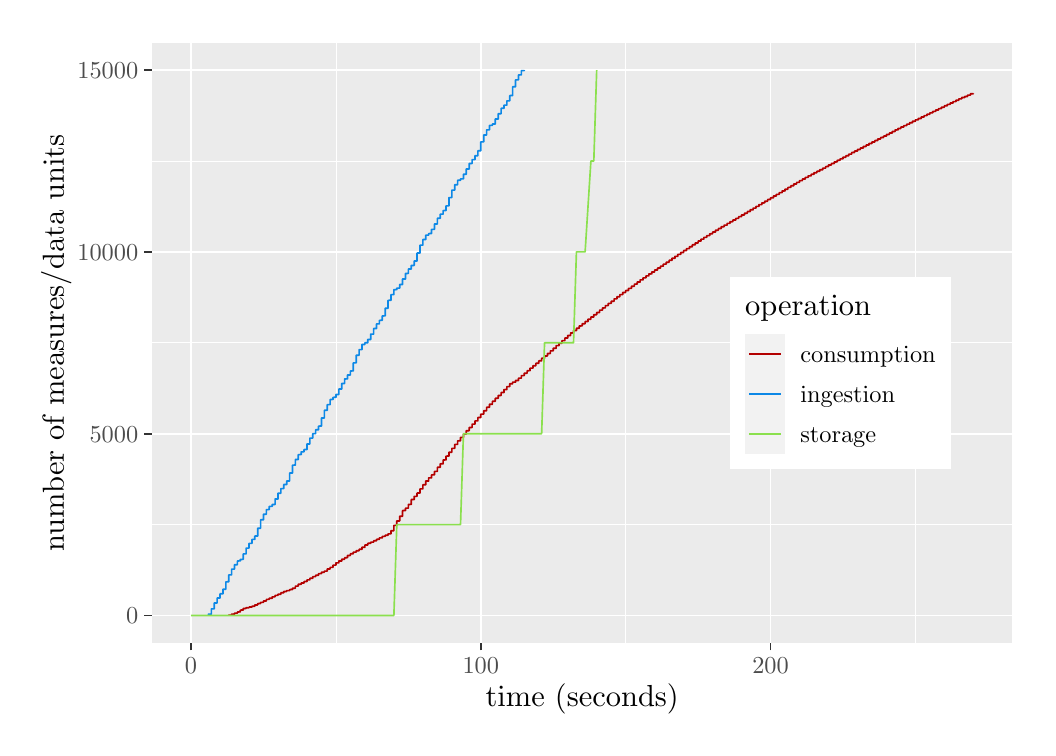
\begin{tikzpicture}[x=1pt,y=1pt]
	\definecolor{fillColor}{RGB}{255,255,255}
	\path[use as bounding box,fill=fillColor,fill opacity=0.00] (0,0) rectangle (361.35,252.94);
	\begin{scope}
	\path[clip] (  0.00,  0.00) rectangle (361.35,252.94);
	\definecolor{drawColor}{RGB}{255,255,255}
	\definecolor{fillColor}{RGB}{255,255,255}
	
	\path[draw=drawColor,line width= 0.6pt,line join=round,line cap=round,fill=fillColor] (  0.00,  0.00) rectangle (361.35,252.94);
	\end{scope}
	\begin{scope}
	\path[clip] ( 44.91, 30.69) rectangle (355.85,247.45);
	\definecolor{fillColor}{gray}{0.92}
	
	\path[fill=fillColor] ( 44.91, 30.69) rectangle (355.85,247.45);
	\definecolor{drawColor}{RGB}{255,255,255}
	
	\path[draw=drawColor,line width= 0.3pt,line join=round] ( 44.91, 73.38) --
		(355.85, 73.38);
	
	\path[draw=drawColor,line width= 0.3pt,line join=round] ( 44.91,139.07) --
		(355.85,139.07);
	
	\path[draw=drawColor,line width= 0.3pt,line join=round] ( 44.91,204.75) --
		(355.85,204.75);
	
	\path[draw=drawColor,line width= 0.3pt,line join=round] (111.39, 30.69) --
		(111.39,247.45);
	
	\path[draw=drawColor,line width= 0.3pt,line join=round] (216.08, 30.69) --
		(216.08,247.45);
	
	\path[draw=drawColor,line width= 0.3pt,line join=round] (320.78, 30.69) --
		(320.78,247.45);
	
	\path[draw=drawColor,line width= 0.6pt,line join=round] ( 44.91, 40.54) --
		(355.85, 40.54);
	
	\path[draw=drawColor,line width= 0.6pt,line join=round] ( 44.91,106.22) --
		(355.85,106.22);
	
	\path[draw=drawColor,line width= 0.6pt,line join=round] ( 44.91,171.91) --
		(355.85,171.91);
	
	\path[draw=drawColor,line width= 0.6pt,line join=round] ( 44.91,237.59) --
		(355.85,237.59);
	
	\path[draw=drawColor,line width= 0.6pt,line join=round] ( 59.04, 30.69) --
		( 59.04,247.45);
	
	\path[draw=drawColor,line width= 0.6pt,line join=round] (163.74, 30.69) --
		(163.74,247.45);
	
	\path[draw=drawColor,line width= 0.6pt,line join=round] (268.43, 30.69) --
		(268.43,247.45);
	\definecolor{drawColor}{RGB}{179,0,0}
	
	\path[draw=drawColor,line width= 0.6pt,line join=round] ( 72.65, 40.55) --
		( 72.65, 40.56) --
		( 72.65, 40.58) --
		( 72.65, 40.59) --
		( 72.65, 40.60) --
		( 72.65, 40.62) --
		( 72.65, 40.63) --
		( 72.65, 40.64) --
		( 72.65, 40.66) --
		( 72.65, 40.67) --
		( 73.70, 40.68) --
		( 73.70, 40.70) --
		( 73.70, 40.71) --
		( 73.70, 40.72) --
		( 73.70, 40.74) --
		( 73.70, 40.75) --
		( 73.70, 40.76) --
		( 73.70, 40.77) --
		( 73.70, 40.79) --
		( 73.70, 40.80) --
		( 73.70, 40.81) --
		( 73.70, 40.83) --
		( 73.70, 40.84) --
		( 73.70, 40.85) --
		( 73.70, 40.87) --
		( 73.70, 40.88) --
		( 73.70, 40.89) --
		( 73.70, 40.91) --
		( 73.70, 40.92) --
		( 73.70, 40.93) --
		( 73.70, 40.95) --
		( 73.70, 40.96) --
		( 73.70, 40.97) --
		( 73.70, 40.99) --
		( 73.70, 41.00) --
		( 73.70, 41.01) --
		( 74.75, 41.02) --
		( 74.75, 41.04) --
		( 74.75, 41.05) --
		( 74.75, 41.06) --
		( 74.75, 41.08) --
		( 74.75, 41.09) --
		( 74.75, 41.10) --
		( 74.75, 41.12) --
		( 74.75, 41.13) --
		( 74.75, 41.14) --
		( 74.75, 41.16) --
		( 74.75, 41.17) --
		( 74.75, 41.18) --
		( 74.75, 41.20) --
		( 74.75, 41.21) --
		( 74.75, 41.22) --
		( 74.75, 41.23) --
		( 74.75, 41.25) --
		( 74.75, 41.26) --
		( 74.75, 41.27) --
		( 74.75, 41.29) --
		( 74.75, 41.30) --
		( 74.75, 41.31) --
		( 74.75, 41.33) --
		( 74.75, 41.34) --
		( 74.75, 41.35) --
		( 74.75, 41.37) --
		( 74.75, 41.38) --
		( 75.79, 41.39) --
		( 75.79, 41.41) --
		( 75.79, 41.42) --
		( 75.79, 41.43) --
		( 75.79, 41.44) --
		( 75.79, 41.46) --
		( 75.79, 41.47) --
		( 75.79, 41.48) --
		( 75.79, 41.50) --
		( 75.79, 41.51) --
		( 75.79, 41.52) --
		( 75.79, 41.54) --
		( 75.79, 41.55) --
		( 75.79, 41.56) --
		( 75.79, 41.58) --
		( 75.79, 41.59) --
		( 75.79, 41.60) --
		( 75.79, 41.62) --
		( 75.79, 41.63) --
		( 75.79, 41.64) --
		( 75.79, 41.66) --
		( 75.79, 41.67) --
		( 75.79, 41.68) --
		( 75.79, 41.69) --
		( 75.79, 41.71) --
		( 75.79, 41.72) --
		( 75.79, 41.73) --
		( 75.79, 41.75) --
		( 75.79, 41.76) --
		( 75.79, 41.77) --
		( 75.79, 41.79) --
		( 75.79, 41.80) --
		( 75.79, 41.81) --
		( 76.84, 41.83) --
		( 76.84, 41.84) --
		( 76.84, 41.85) --
		( 76.84, 41.87) --
		( 76.84, 41.88) --
		( 76.84, 41.89) --
		( 76.84, 41.90) --
		( 76.84, 41.92) --
		( 76.84, 41.93) --
		( 76.84, 41.94) --
		( 76.84, 41.96) --
		( 76.84, 41.97) --
		( 76.84, 41.98) --
		( 76.84, 42.00) --
		( 76.84, 42.01) --
		( 76.84, 42.02) --
		( 76.84, 42.04) --
		( 76.84, 42.05) --
		( 76.84, 42.06) --
		( 76.84, 42.08) --
		( 76.84, 42.09) --
		( 76.84, 42.10) --
		( 76.84, 42.11) --
		( 76.84, 42.13) --
		( 76.84, 42.14) --
		( 76.84, 42.15) --
		( 76.84, 42.17) --
		( 76.84, 42.18) --
		( 76.84, 42.19) --
		( 76.84, 42.21) --
		( 76.84, 42.22) --
		( 76.84, 42.23) --
		( 76.84, 42.25) --
		( 76.84, 42.26) --
		( 76.84, 42.27) --
		( 76.84, 42.29) --
		( 76.84, 42.30) --
		( 76.84, 42.31) --
		( 76.84, 42.33) --
		( 76.84, 42.34) --
		( 76.84, 42.35) --
		( 76.84, 42.36) --
		( 76.84, 42.38) --
		( 76.84, 42.39) --
		( 76.84, 42.40) --
		( 76.84, 42.42) --
		( 76.84, 42.43) --
		( 76.84, 42.44) --
		( 76.84, 42.46) --
		( 76.84, 42.47) --
		( 76.84, 42.48) --
		( 77.89, 42.50) --
		( 77.89, 42.51) --
		( 77.89, 42.52) --
		( 77.89, 42.54) --
		( 77.89, 42.55) --
		( 77.89, 42.56) --
		( 77.89, 42.57) --
		( 77.89, 42.59) --
		( 77.89, 42.60) --
		( 77.89, 42.61) --
		( 77.89, 42.63) --
		( 77.89, 42.64) --
		( 77.89, 42.65) --
		( 77.89, 42.67) --
		( 77.89, 42.68) --
		( 77.89, 42.69) --
		( 77.89, 42.71) --
		( 77.89, 42.72) --
		( 77.89, 42.73) --
		( 77.89, 42.75) --
		( 77.89, 42.76) --
		( 77.89, 42.77) --
		( 77.89, 42.78) --
		( 77.89, 42.80) --
		( 77.89, 42.81) --
		( 77.89, 42.82) --
		( 77.89, 42.84) --
		( 77.89, 42.85) --
		( 77.89, 42.86) --
		( 77.89, 42.88) --
		( 77.89, 42.89) --
		( 77.89, 42.90) --
		( 77.89, 42.92) --
		( 77.89, 42.93) --
		( 77.89, 42.94) --
		( 77.89, 42.96) --
		( 77.89, 42.97) --
		( 77.89, 42.98) --
		( 77.89, 43.00) --
		( 77.89, 43.01) --
		( 77.89, 43.02) --
		( 77.89, 43.03) --
		( 78.93, 43.05) --
		( 78.93, 43.06) --
		( 78.93, 43.07) --
		( 78.93, 43.09) --
		( 78.93, 43.10) --
		( 78.93, 43.11) --
		( 78.93, 43.13) --
		( 78.93, 43.14) --
		( 78.93, 43.15) --
		( 78.93, 43.17) --
		( 78.93, 43.18) --
		( 78.93, 43.19) --
		( 78.93, 43.21) --
		( 78.93, 43.22) --
		( 78.93, 43.23) --
		( 78.93, 43.24) --
		( 78.93, 43.26) --
		( 78.93, 43.27) --
		( 78.93, 43.28) --
		( 78.93, 43.30) --
		( 78.93, 43.31) --
		( 78.93, 43.32) --
		( 78.93, 43.34) --
		( 79.98, 43.35) --
		( 79.98, 43.36) --
		( 79.98, 43.38) --
		( 79.98, 43.39) --
		( 79.98, 43.40) --
		( 79.98, 43.42) --
		( 79.98, 43.43) --
		( 79.98, 43.44) --
		( 79.98, 43.45) --
		( 79.98, 43.47) --
		( 79.98, 43.48) --
		( 79.98, 43.49) --
		( 79.98, 43.51) --
		( 79.98, 43.52) --
		( 79.98, 43.53) --
		( 79.98, 43.55) --
		( 79.98, 43.56) --
		( 79.98, 43.57) --
		( 81.03, 43.59) --
		( 81.03, 43.60) --
		( 81.03, 43.61) --
		( 81.03, 43.63) --
		( 81.03, 43.64) --
		( 81.03, 43.65) --
		( 81.03, 43.67) --
		( 81.03, 43.68) --
		( 81.03, 43.69) --
		( 81.03, 43.70) --
		( 81.03, 43.72) --
		( 81.03, 43.73) --
		( 81.03, 43.74) --
		( 81.03, 43.76) --
		( 81.03, 43.77) --
		( 81.03, 43.78) --
		( 81.03, 43.80) --
		( 81.03, 43.81) --
		( 81.03, 43.82) --
		( 81.03, 43.84) --
		( 81.03, 43.85) --
		( 81.03, 43.86) --
		( 81.03, 43.88) --
		( 81.03, 43.89) --
		( 82.08, 43.90) --
		( 82.08, 43.91) --
		( 82.08, 43.93) --
		( 82.08, 43.94) --
		( 82.08, 43.95) --
		( 82.08, 43.97) --
		( 82.08, 43.98) --
		( 82.08, 43.99) --
		( 82.08, 44.01) --
		( 82.08, 44.02) --
		( 82.08, 44.03) --
		( 82.08, 44.05) --
		( 82.08, 44.06) --
		( 82.08, 44.07) --
		( 82.08, 44.09) --
		( 82.08, 44.10) --
		( 82.08, 44.11) --
		( 82.08, 44.12) --
		( 82.08, 44.14) --
		( 82.08, 44.15) --
		( 82.08, 44.16) --
		( 82.08, 44.18) --
		( 82.08, 44.19) --
		( 82.08, 44.20) --
		( 82.08, 44.22) --
		( 82.08, 44.23) --
		( 82.08, 44.24) --
		( 82.08, 44.26) --
		( 82.08, 44.27) --
		( 82.08, 44.28) --
		( 82.08, 44.30) --
		( 82.08, 44.31) --
		( 82.08, 44.32) --
		( 83.12, 44.34) --
		( 83.12, 44.35) --
		( 83.12, 44.36) --
		( 83.12, 44.37) --
		( 83.12, 44.39) --
		( 83.12, 44.40) --
		( 83.12, 44.41) --
		( 83.12, 44.43) --
		( 83.12, 44.44) --
		( 83.12, 44.45) --
		( 83.12, 44.47) --
		( 83.12, 44.48) --
		( 83.12, 44.49) --
		( 83.12, 44.51) --
		( 83.12, 44.52) --
		( 83.12, 44.53) --
		( 83.12, 44.55) --
		( 83.12, 44.56) --
		( 83.12, 44.57) --
		( 83.12, 44.58) --
		( 83.12, 44.60) --
		( 83.12, 44.61) --
		( 83.12, 44.62) --
		( 83.12, 44.64) --
		( 83.12, 44.65) --
		( 83.12, 44.66) --
		( 83.12, 44.68) --
		( 83.12, 44.69) --
		( 83.12, 44.70) --
		( 83.12, 44.72) --
		( 83.12, 44.73) --
		( 83.12, 44.74) --
		( 83.12, 44.76) --
		( 83.12, 44.77) --
		( 83.12, 44.78) --
		( 83.12, 44.79) --
		( 83.12, 44.81) --
		( 83.12, 44.82) --
		( 83.12, 44.83) --
		( 84.17, 44.85) --
		( 84.17, 44.86) --
		( 84.17, 44.87) --
		( 84.17, 44.89) --
		( 84.17, 44.90) --
		( 84.17, 44.91) --
		( 84.17, 44.93) --
		( 84.17, 44.94) --
		( 84.17, 44.95) --
		( 84.17, 44.97) --
		( 84.17, 44.98) --
		( 84.17, 44.99) --
		( 84.17, 45.01) --
		( 84.17, 45.02) --
		( 84.17, 45.03) --
		( 84.17, 45.04) --
		( 84.17, 45.06) --
		( 84.17, 45.07) --
		( 84.17, 45.08) --
		( 84.17, 45.10) --
		( 84.17, 45.11) --
		( 84.17, 45.12) --
		( 84.17, 45.14) --
		( 84.17, 45.15) --
		( 84.17, 45.16) --
		( 84.17, 45.18) --
		( 84.17, 45.19) --
		( 84.17, 45.20) --
		( 84.17, 45.22) --
		( 84.17, 45.23) --
		( 84.17, 45.24) --
		( 84.17, 45.25) --
		( 85.22, 45.27) --
		( 85.22, 45.28) --
		( 85.22, 45.29) --
		( 85.22, 45.31) --
		( 85.22, 45.32) --
		( 85.22, 45.33) --
		( 85.22, 45.35) --
		( 85.22, 45.36) --
		( 85.22, 45.37) --
		( 85.22, 45.39) --
		( 85.22, 45.40) --
		( 85.22, 45.41) --
		( 85.22, 45.43) --
		( 85.22, 45.44) --
		( 85.22, 45.45) --
		( 85.22, 45.46) --
		( 85.22, 45.48) --
		( 85.22, 45.49) --
		( 85.22, 45.50) --
		( 85.22, 45.52) --
		( 85.22, 45.53) --
		( 85.22, 45.54) --
		( 85.22, 45.56) --
		( 85.22, 45.57) --
		( 85.22, 45.58) --
		( 85.22, 45.60) --
		( 85.22, 45.61) --
		( 85.22, 45.62) --
		( 85.22, 45.64) --
		( 85.22, 45.65) --
		( 85.22, 45.66) --
		( 85.22, 45.68) --
		( 85.22, 45.69) --
		( 85.22, 45.70) --
		( 85.22, 45.71) --
		( 85.22, 45.73) --
		( 85.22, 45.74) --
		( 85.22, 45.75) --
		( 85.22, 45.77) --
		( 85.22, 45.78) --
		( 86.26, 45.79) --
		( 86.26, 45.81) --
		( 86.26, 45.82) --
		( 86.26, 45.83) --
		( 86.26, 45.85) --
		( 86.26, 45.86) --
		( 86.26, 45.87) --
		( 86.26, 45.89) --
		( 86.26, 45.90) --
		( 86.26, 45.91) --
		( 86.26, 45.92) --
		( 86.26, 45.94) --
		( 86.26, 45.95) --
		( 86.26, 45.96) --
		( 86.26, 45.98) --
		( 86.26, 45.99) --
		( 86.26, 46.00) --
		( 86.26, 46.02) --
		( 86.26, 46.03) --
		( 86.26, 46.04) --
		( 86.26, 46.06) --
		( 86.26, 46.07) --
		( 86.26, 46.08) --
		( 86.26, 46.10) --
		( 86.26, 46.11) --
		( 86.26, 46.12) --
		( 86.26, 46.13) --
		( 86.26, 46.15) --
		( 86.26, 46.16) --
		( 86.26, 46.17) --
		( 86.26, 46.19) --
		( 86.26, 46.20) --
		( 86.26, 46.21) --
		( 86.26, 46.23) --
		( 86.26, 46.24) --
		( 86.26, 46.25) --
		( 86.26, 46.27) --
		( 86.26, 46.28) --
		( 86.26, 46.29) --
		( 86.26, 46.31) --
		( 86.26, 46.32) --
		( 86.26, 46.33) --
		( 86.26, 46.35) --
		( 87.31, 46.36) --
		( 87.31, 46.37) --
		( 87.31, 46.38) --
		( 87.31, 46.40) --
		( 87.31, 46.41) --
		( 87.31, 46.42) --
		( 87.31, 46.44) --
		( 87.31, 46.45) --
		( 87.31, 46.46) --
		( 87.31, 46.48) --
		( 87.31, 46.49) --
		( 87.31, 46.50) --
		( 87.31, 46.52) --
		( 87.31, 46.53) --
		( 87.31, 46.54) --
		( 87.31, 46.56) --
		( 87.31, 46.57) --
		( 87.31, 46.58) --
		( 87.31, 46.59) --
		( 87.31, 46.61) --
		( 87.31, 46.62) --
		( 87.31, 46.63) --
		( 87.31, 46.65) --
		( 87.31, 46.66) --
		( 87.31, 46.67) --
		( 87.31, 46.69) --
		( 87.31, 46.70) --
		( 87.31, 46.71) --
		( 87.31, 46.73) --
		( 87.31, 46.74) --
		( 87.31, 46.75) --
		( 88.36, 46.77) --
		( 88.36, 46.78) --
		( 88.36, 46.79) --
		( 88.36, 46.80) --
		( 88.36, 46.82) --
		( 88.36, 46.83) --
		( 88.36, 46.84) --
		( 88.36, 46.86) --
		( 88.36, 46.87) --
		( 88.36, 46.88) --
		( 88.36, 46.90) --
		( 88.36, 46.91) --
		( 88.36, 46.92) --
		( 88.36, 46.94) --
		( 88.36, 46.95) --
		( 88.36, 46.96) --
		( 88.36, 46.98) --
		( 88.36, 46.99) --
		( 88.36, 47.00) --
		( 88.36, 47.02) --
		( 88.36, 47.03) --
		( 88.36, 47.04) --
		( 88.36, 47.05) --
		( 88.36, 47.07) --
		( 88.36, 47.08) --
		( 88.36, 47.09) --
		( 88.36, 47.11) --
		( 88.36, 47.12) --
		( 88.36, 47.13) --
		( 88.36, 47.15) --
		( 88.36, 47.16) --
		( 88.36, 47.17) --
		( 88.36, 47.19) --
		( 88.36, 47.20) --
		( 88.36, 47.21) --
		( 88.36, 47.23) --
		( 88.36, 47.24) --
		( 88.36, 47.25) --
		( 88.36, 47.26) --
		( 89.40, 47.28) --
		( 89.40, 47.29) --
		( 89.40, 47.30) --
		( 89.40, 47.32) --
		( 89.40, 47.33) --
		( 89.40, 47.34) --
		( 89.40, 47.36) --
		( 89.40, 47.37) --
		( 89.40, 47.38) --
		( 89.40, 47.40) --
		( 89.40, 47.41) --
		( 89.40, 47.42) --
		( 89.40, 47.44) --
		( 89.40, 47.45) --
		( 89.40, 47.46) --
		( 89.40, 47.47) --
		( 89.40, 47.49) --
		( 89.40, 47.50) --
		( 89.40, 47.51) --
		( 89.40, 47.53) --
		( 89.40, 47.54) --
		( 89.40, 47.55) --
		( 89.40, 47.57) --
		( 89.40, 47.58) --
		( 89.40, 47.59) --
		( 89.40, 47.61) --
		( 89.40, 47.62) --
		( 89.40, 47.63) --
		( 89.40, 47.65) --
		( 89.40, 47.66) --
		( 89.40, 47.67) --
		( 89.40, 47.68) --
		( 89.40, 47.70) --
		( 89.40, 47.71) --
		( 89.40, 47.72) --
		( 89.40, 47.74) --
		( 89.40, 47.75) --
		( 89.40, 47.76) --
		( 89.40, 47.78) --
		( 90.45, 47.79) --
		( 90.45, 47.80) --
		( 90.45, 47.82) --
		( 90.45, 47.83) --
		( 90.45, 47.84) --
		( 90.45, 47.86) --
		( 90.45, 47.87) --
		( 90.45, 47.88) --
		( 90.45, 47.90) --
		( 90.45, 47.91) --
		( 90.45, 47.92) --
		( 90.45, 47.93) --
		( 90.45, 47.95) --
		( 90.45, 47.96) --
		( 90.45, 47.97) --
		( 90.45, 47.99) --
		( 90.45, 48.00) --
		( 90.45, 48.01) --
		( 90.45, 48.03) --
		( 90.45, 48.04) --
		( 90.45, 48.05) --
		( 90.45, 48.07) --
		( 90.45, 48.08) --
		( 90.45, 48.09) --
		( 90.45, 48.11) --
		( 90.45, 48.12) --
		( 90.45, 48.13) --
		( 90.45, 48.14) --
		( 90.45, 48.16) --
		( 90.45, 48.17) --
		( 90.45, 48.18) --
		( 91.50, 48.20) --
		( 91.50, 48.21) --
		( 91.50, 48.22) --
		( 91.50, 48.24) --
		( 91.50, 48.25) --
		( 91.50, 48.26) --
		( 91.50, 48.28) --
		( 91.50, 48.29) --
		( 91.50, 48.30) --
		( 91.50, 48.32) --
		( 91.50, 48.33) --
		( 91.50, 48.34) --
		( 91.50, 48.35) --
		( 91.50, 48.37) --
		( 91.50, 48.38) --
		( 91.50, 48.39) --
		( 91.50, 48.41) --
		( 91.50, 48.42) --
		( 91.50, 48.43) --
		( 91.50, 48.45) --
		( 91.50, 48.46) --
		( 91.50, 48.47) --
		( 91.50, 48.49) --
		( 91.50, 48.50) --
		( 91.50, 48.51) --
		( 91.50, 48.53) --
		( 91.50, 48.54) --
		( 91.50, 48.55) --
		( 91.50, 48.57) --
		( 91.50, 48.58) --
		( 91.50, 48.59) --
		( 91.50, 48.60) --
		( 91.50, 48.62) --
		( 91.50, 48.63) --
		( 91.50, 48.64) --
		( 91.50, 48.66) --
		( 91.50, 48.67) --
		( 91.50, 48.68) --
		( 91.50, 48.70) --
		( 91.50, 48.71) --
		( 91.50, 48.72) --
		( 91.50, 48.74) --
		( 92.54, 48.75) --
		( 92.54, 48.76) --
		( 92.54, 48.78) --
		( 92.54, 48.79) --
		( 92.54, 48.80) --
		( 92.54, 48.81) --
		( 92.54, 48.83) --
		( 92.54, 48.84) --
		( 92.54, 48.85) --
		( 92.54, 48.87) --
		( 92.54, 48.88) --
		( 92.54, 48.89) --
		( 92.54, 48.91) --
		( 92.54, 48.92) --
		( 92.54, 48.93) --
		( 92.54, 48.95) --
		( 92.54, 48.96) --
		( 92.54, 48.97) --
		( 92.54, 48.99) --
		( 92.54, 49.00) --
		( 92.54, 49.01) --
		( 92.54, 49.02) --
		( 92.54, 49.04) --
		( 92.54, 49.05) --
		( 92.54, 49.06) --
		( 92.54, 49.08) --
		( 92.54, 49.09) --
		( 92.54, 49.10) --
		( 92.54, 49.12) --
		( 92.54, 49.13) --
		( 92.54, 49.14) --
		( 92.54, 49.16) --
		( 92.54, 49.17) --
		( 92.54, 49.18) --
		( 92.54, 49.20) --
		( 93.59, 49.21) --
		( 93.59, 49.22) --
		( 93.59, 49.24) --
		( 93.59, 49.25) --
		( 93.59, 49.26) --
		( 93.59, 49.27) --
		( 93.59, 49.29) --
		( 93.59, 49.30) --
		( 93.59, 49.31) --
		( 93.59, 49.33) --
		( 93.59, 49.34) --
		( 93.59, 49.35) --
		( 93.59, 49.37) --
		( 93.59, 49.38) --
		( 93.59, 49.39) --
		( 93.59, 49.41) --
		( 93.59, 49.42) --
		( 93.59, 49.43) --
		( 93.59, 49.45) --
		( 93.59, 49.46) --
		( 93.59, 49.47) --
		( 93.59, 49.48) --
		( 93.59, 49.50) --
		( 93.59, 49.51) --
		( 94.64, 49.52) --
		( 94.64, 49.54) --
		( 94.64, 49.55) --
		( 94.64, 49.56) --
		( 94.64, 49.58) --
		( 94.64, 49.59) --
		( 94.64, 49.60) --
		( 94.64, 49.62) --
		( 94.64, 49.63) --
		( 94.64, 49.64) --
		( 94.64, 49.66) --
		( 94.64, 49.67) --
		( 94.64, 49.68) --
		( 94.64, 49.69) --
		( 94.64, 49.71) --
		( 94.64, 49.72) --
		( 94.64, 49.73) --
		( 94.64, 49.75) --
		( 94.64, 49.76) --
		( 94.64, 49.77) --
		( 94.64, 49.79) --
		( 94.64, 49.80) --
		( 94.64, 49.81) --
		( 94.64, 49.83) --
		( 94.64, 49.84) --
		( 94.64, 49.85) --
		( 94.64, 49.87) --
		( 94.64, 49.88) --
		( 94.64, 49.89) --
		( 95.69, 49.91) --
		( 95.69, 49.92) --
		( 95.69, 49.93) --
		( 95.69, 49.94) --
		( 95.69, 49.96) --
		( 95.69, 49.97) --
		( 95.69, 49.98) --
		( 95.69, 50.00) --
		( 95.69, 50.01) --
		( 95.69, 50.02) --
		( 95.69, 50.04) --
		( 95.69, 50.05) --
		( 95.69, 50.06) --
		( 95.69, 50.08) --
		( 95.69, 50.09) --
		( 95.69, 50.10) --
		( 95.69, 50.12) --
		( 95.69, 50.13) --
		( 95.69, 50.14) --
		( 95.69, 50.15) --
		( 95.69, 50.17) --
		( 95.69, 50.18) --
		( 95.69, 50.19) --
		( 95.69, 50.21) --
		( 95.69, 50.22) --
		( 95.69, 50.23) --
		( 95.69, 50.25) --
		( 95.69, 50.26) --
		( 95.69, 50.27) --
		( 95.69, 50.29) --
		( 95.69, 50.30) --
		( 95.69, 50.31) --
		( 95.69, 50.33) --
		( 95.69, 50.34) --
		( 95.69, 50.35) --
		( 96.73, 50.36) --
		( 96.73, 50.38) --
		( 96.73, 50.39) --
		( 96.73, 50.40) --
		( 96.73, 50.42) --
		( 96.73, 50.43) --
		( 96.73, 50.44) --
		( 96.73, 50.46) --
		( 96.73, 50.47) --
		( 96.73, 50.48) --
		( 96.73, 50.50) --
		( 96.73, 50.51) --
		( 96.73, 50.52) --
		( 96.73, 50.54) --
		( 96.73, 50.55) --
		( 96.73, 50.56) --
		( 96.73, 50.58) --
		( 96.73, 50.59) --
		( 96.73, 50.60) --
		( 96.73, 50.61) --
		( 96.73, 50.63) --
		( 96.73, 50.64) --
		( 96.73, 50.65) --
		( 96.73, 50.67) --
		( 96.73, 50.68) --
		( 96.73, 50.69) --
		( 96.73, 50.71) --
		( 96.73, 50.72) --
		( 96.73, 50.73) --
		( 96.73, 50.75) --
		( 96.73, 50.76) --
		( 96.73, 50.77) --
		( 96.73, 50.79) --
		( 96.73, 50.80) --
		( 96.73, 50.81) --
		( 96.73, 50.82) --
		( 96.73, 50.84) --
		( 96.73, 50.85) --
		( 96.73, 50.86) --
		( 96.73, 50.88) --
		( 96.73, 50.89) --
		( 96.73, 50.90) --
		( 96.73, 50.92) --
		( 96.73, 50.93) --
		( 96.73, 50.94) --
		( 96.73, 50.96) --
		( 96.73, 50.97) --
		( 96.73, 50.98) --
		( 96.73, 51.00) --
		( 96.73, 51.01) --
		( 96.73, 51.02) --
		( 96.73, 51.03) --
		( 96.73, 51.05) --
		( 96.73, 51.06) --
		( 96.73, 51.07) --
		( 96.73, 51.09) --
		( 96.73, 51.10) --
		( 96.73, 51.11) --
		( 96.73, 51.13) --
		( 97.78, 51.14) --
		( 97.78, 51.15) --
		( 97.78, 51.17) --
		( 97.78, 51.18) --
		( 97.78, 51.19) --
		( 97.78, 51.21) --
		( 97.78, 51.22) --
		( 97.78, 51.23) --
		( 97.78, 51.25) --
		( 97.78, 51.26) --
		( 97.78, 51.27) --
		( 97.78, 51.28) --
		( 97.78, 51.30) --
		( 97.78, 51.31) --
		( 97.78, 51.32) --
		( 97.78, 51.34) --
		( 97.78, 51.35) --
		( 97.78, 51.36) --
		( 97.78, 51.38) --
		( 97.78, 51.39) --
		( 97.78, 51.40) --
		( 97.78, 51.42) --
		( 97.78, 51.43) --
		( 97.78, 51.44) --
		( 97.78, 51.46) --
		( 97.78, 51.47) --
		( 97.78, 51.48) --
		( 97.78, 51.49) --
		( 97.78, 51.51) --
		( 97.78, 51.52) --
		( 97.78, 51.53) --
		( 97.78, 51.55) --
		( 97.78, 51.56) --
		( 97.78, 51.57) --
		( 97.78, 51.59) --
		( 97.78, 51.60) --
		( 97.78, 51.61) --
		( 97.78, 51.63) --
		( 97.78, 51.64) --
		( 97.78, 51.65) --
		( 97.78, 51.67) --
		( 97.78, 51.68) --
		( 97.78, 51.69) --
		( 97.78, 51.70) --
		( 97.78, 51.72) --
		( 97.78, 51.73) --
		( 97.78, 51.74) --
		( 97.78, 51.76) --
		( 97.78, 51.77) --
		( 97.78, 51.78) --
		( 97.78, 51.80) --
		( 97.78, 51.81) --
		( 98.83, 51.82) --
		( 98.83, 51.84) --
		( 98.83, 51.85) --
		( 98.83, 51.86) --
		( 98.83, 51.88) --
		( 98.83, 51.89) --
		( 98.83, 51.90) --
		( 98.83, 51.92) --
		( 98.83, 51.93) --
		( 98.83, 51.94) --
		( 98.83, 51.95) --
		( 98.83, 51.97) --
		( 98.83, 51.98) --
		( 98.83, 51.99) --
		( 98.83, 52.01) --
		( 98.83, 52.02) --
		( 98.83, 52.03) --
		( 98.83, 52.05) --
		( 98.83, 52.06) --
		( 98.83, 52.07) --
		( 98.83, 52.09) --
		( 98.83, 52.10) --
		( 98.83, 52.11) --
		( 98.83, 52.13) --
		( 98.83, 52.14) --
		( 98.83, 52.15) --
		( 98.83, 52.16) --
		( 98.83, 52.18) --
		( 98.83, 52.19) --
		( 98.83, 52.20) --
		( 98.83, 52.22) --
		( 98.83, 52.23) --
		( 98.83, 52.24) --
		( 98.83, 52.26) --
		( 99.87, 52.27) --
		( 99.87, 52.28) --
		( 99.87, 52.30) --
		( 99.87, 52.31) --
		( 99.87, 52.32) --
		( 99.87, 52.34) --
		( 99.87, 52.35) --
		( 99.87, 52.36) --
		( 99.87, 52.37) --
		( 99.87, 52.39) --
		( 99.87, 52.40) --
		( 99.87, 52.41) --
		( 99.87, 52.43) --
		( 99.87, 52.44) --
		( 99.87, 52.45) --
		( 99.87, 52.47) --
		( 99.87, 52.48) --
		( 99.87, 52.49) --
		( 99.87, 52.51) --
		( 99.87, 52.52) --
		( 99.87, 52.53) --
		( 99.87, 52.55) --
		( 99.87, 52.56) --
		( 99.87, 52.57) --
		( 99.87, 52.59) --
		( 99.87, 52.60) --
		( 99.87, 52.61) --
		( 99.87, 52.62) --
		( 99.87, 52.64) --
		( 99.87, 52.65) --
		( 99.87, 52.66) --
		( 99.87, 52.68) --
		( 99.87, 52.69) --
		( 99.87, 52.70) --
		( 99.87, 52.72) --
		( 99.87, 52.73) --
		( 99.87, 52.74) --
		( 99.87, 52.76) --
		( 99.87, 52.77) --
		( 99.87, 52.78) --
		( 99.87, 52.80) --
		(100.92, 52.81) --
		(100.92, 52.82) --
		(100.92, 52.83) --
		(100.92, 52.85) --
		(100.92, 52.86) --
		(100.92, 52.87) --
		(100.92, 52.89) --
		(100.92, 52.90) --
		(100.92, 52.91) --
		(100.92, 52.93) --
		(100.92, 52.94) --
		(100.92, 52.95) --
		(100.92, 52.97) --
		(100.92, 52.98) --
		(100.92, 52.99) --
		(100.92, 53.01) --
		(100.92, 53.02) --
		(100.92, 53.03) --
		(100.92, 53.04) --
		(100.92, 53.06) --
		(100.92, 53.07) --
		(100.92, 53.08) --
		(100.92, 53.10) --
		(100.92, 53.11) --
		(100.92, 53.12) --
		(100.92, 53.14) --
		(100.92, 53.15) --
		(100.92, 53.16) --
		(100.92, 53.18) --
		(100.92, 53.19) --
		(100.92, 53.20) --
		(100.92, 53.22) --
		(100.92, 53.23) --
		(100.92, 53.24) --
		(100.92, 53.26) --
		(100.92, 53.27) --
		(100.92, 53.28) --
		(100.92, 53.29) --
		(100.92, 53.31) --
		(100.92, 53.32) --
		(100.92, 53.33) --
		(100.92, 53.35) --
		(100.92, 53.36) --
		(100.92, 53.37) --
		(100.92, 53.39) --
		(100.92, 53.40) --
		(101.97, 53.41) --
		(101.97, 53.43) --
		(101.97, 53.44) --
		(101.97, 53.45) --
		(101.97, 53.47) --
		(101.97, 53.48) --
		(101.97, 53.49) --
		(101.97, 53.50) --
		(101.97, 53.52) --
		(101.97, 53.53) --
		(101.97, 53.54) --
		(101.97, 53.56) --
		(101.97, 53.57) --
		(101.97, 53.58) --
		(101.97, 53.60) --
		(101.97, 53.61) --
		(101.97, 53.62) --
		(101.97, 53.64) --
		(101.97, 53.65) --
		(101.97, 53.66) --
		(101.97, 53.68) --
		(101.97, 53.69) --
		(101.97, 53.70) --
		(101.97, 53.71) --
		(101.97, 53.73) --
		(101.97, 53.74) --
		(101.97, 53.75) --
		(101.97, 53.77) --
		(101.97, 53.78) --
		(101.97, 53.79) --
		(101.97, 53.81) --
		(101.97, 53.82) --
		(101.97, 53.83) --
		(101.97, 53.85) --
		(101.97, 53.86) --
		(101.97, 53.87) --
		(101.97, 53.89) --
		(101.97, 53.90) --
		(101.97, 53.91) --
		(101.97, 53.93) --
		(101.97, 53.94) --
		(101.97, 53.95) --
		(101.97, 53.96) --
		(101.97, 53.98) --
		(103.01, 53.99) --
		(103.01, 54.00) --
		(103.01, 54.02) --
		(103.01, 54.03) --
		(103.01, 54.04) --
		(103.01, 54.06) --
		(103.01, 54.07) --
		(103.01, 54.08) --
		(103.01, 54.10) --
		(103.01, 54.11) --
		(103.01, 54.12) --
		(103.01, 54.14) --
		(103.01, 54.15) --
		(103.01, 54.16) --
		(103.01, 54.17) --
		(103.01, 54.19) --
		(103.01, 54.20) --
		(103.01, 54.21) --
		(103.01, 54.23) --
		(103.01, 54.24) --
		(103.01, 54.25) --
		(103.01, 54.27) --
		(103.01, 54.28) --
		(103.01, 54.29) --
		(103.01, 54.31) --
		(103.01, 54.32) --
		(103.01, 54.33) --
		(103.01, 54.35) --
		(103.01, 54.36) --
		(103.01, 54.37) --
		(103.01, 54.38) --
		(103.01, 54.40) --
		(103.01, 54.41) --
		(103.01, 54.42) --
		(103.01, 54.44) --
		(103.01, 54.45) --
		(103.01, 54.46) --
		(103.01, 54.48) --
		(103.01, 54.49) --
		(103.01, 54.50) --
		(103.01, 54.52) --
		(103.01, 54.53) --
		(103.01, 54.54) --
		(103.01, 54.56) --
		(103.01, 54.57) --
		(104.06, 54.58) --
		(104.06, 54.60) --
		(104.06, 54.61) --
		(104.06, 54.62) --
		(104.06, 54.63) --
		(104.06, 54.65) --
		(104.06, 54.66) --
		(104.06, 54.67) --
		(104.06, 54.69) --
		(104.06, 54.70) --
		(104.06, 54.71) --
		(104.06, 54.73) --
		(104.06, 54.74) --
		(104.06, 54.75) --
		(104.06, 54.77) --
		(104.06, 54.78) --
		(104.06, 54.79) --
		(104.06, 54.81) --
		(104.06, 54.82) --
		(104.06, 54.83) --
		(104.06, 54.84) --
		(104.06, 54.86) --
		(104.06, 54.87) --
		(104.06, 54.88) --
		(104.06, 54.90) --
		(104.06, 54.91) --
		(104.06, 54.92) --
		(104.06, 54.94) --
		(104.06, 54.95) --
		(104.06, 54.96) --
		(104.06, 54.98) --
		(104.06, 54.99) --
		(104.06, 55.00) --
		(104.06, 55.02) --
		(104.06, 55.03) --
		(104.06, 55.04) --
		(104.06, 55.05) --
		(104.06, 55.07) --
		(104.06, 55.08) --
		(105.11, 55.09) --
		(105.11, 55.11) --
		(105.11, 55.12) --
		(105.11, 55.13) --
		(105.11, 55.15) --
		(105.11, 55.16) --
		(105.11, 55.17) --
		(105.11, 55.19) --
		(105.11, 55.20) --
		(105.11, 55.21) --
		(105.11, 55.23) --
		(105.11, 55.24) --
		(105.11, 55.25) --
		(105.11, 55.26) --
		(105.11, 55.28) --
		(105.11, 55.29) --
		(105.11, 55.30) --
		(105.11, 55.32) --
		(105.11, 55.33) --
		(105.11, 55.34) --
		(105.11, 55.36) --
		(105.11, 55.37) --
		(105.11, 55.38) --
		(105.11, 55.40) --
		(105.11, 55.41) --
		(105.11, 55.42) --
		(105.11, 55.44) --
		(105.11, 55.45) --
		(105.11, 55.46) --
		(105.11, 55.48) --
		(105.11, 55.49) --
		(105.11, 55.50) --
		(105.11, 55.51) --
		(105.11, 55.53) --
		(105.11, 55.54) --
		(105.11, 55.55) --
		(105.11, 55.57) --
		(105.11, 55.58) --
		(105.11, 55.59) --
		(105.11, 55.61) --
		(105.11, 55.62) --
		(105.11, 55.63) --
		(105.11, 55.65) --
		(105.11, 55.66) --
		(106.16, 55.67) --
		(106.16, 55.69) --
		(106.16, 55.70) --
		(106.16, 55.71) --
		(106.16, 55.72) --
		(106.16, 55.74) --
		(106.16, 55.75) --
		(106.16, 55.76) --
		(106.16, 55.78) --
		(106.16, 55.79) --
		(106.16, 55.80) --
		(106.16, 55.82) --
		(106.16, 55.83) --
		(106.16, 55.84) --
		(106.16, 55.86) --
		(106.16, 55.87) --
		(106.16, 55.88) --
		(106.16, 55.90) --
		(106.16, 55.91) --
		(106.16, 55.92) --
		(106.16, 55.93) --
		(106.16, 55.95) --
		(106.16, 55.96) --
		(106.16, 55.97) --
		(106.16, 55.99) --
		(106.16, 56.00) --
		(106.16, 56.01) --
		(106.16, 56.03) --
		(106.16, 56.04) --
		(106.16, 56.05) --
		(106.16, 56.07) --
		(106.16, 56.08) --
		(106.16, 56.09) --
		(106.16, 56.11) --
		(106.16, 56.12) --
		(106.16, 56.13) --
		(106.16, 56.15) --
		(106.16, 56.16) --
		(107.20, 56.17) --
		(107.20, 56.18) --
		(107.20, 56.20) --
		(107.20, 56.21) --
		(107.20, 56.22) --
		(107.20, 56.24) --
		(107.20, 56.25) --
		(107.20, 56.26) --
		(107.20, 56.28) --
		(107.20, 56.29) --
		(107.20, 56.30) --
		(107.20, 56.32) --
		(107.20, 56.33) --
		(107.20, 56.34) --
		(107.20, 56.36) --
		(107.20, 56.37) --
		(107.20, 56.38) --
		(107.20, 56.39) --
		(107.20, 56.41) --
		(107.20, 56.42) --
		(107.20, 56.43) --
		(107.20, 56.45) --
		(107.20, 56.46) --
		(107.20, 56.47) --
		(107.20, 56.49) --
		(107.20, 56.50) --
		(107.20, 56.51) --
		(107.20, 56.53) --
		(107.20, 56.54) --
		(107.20, 56.55) --
		(107.20, 56.57) --
		(108.25, 56.58) --
		(108.25, 56.59) --
		(108.25, 56.60) --
		(108.25, 56.62) --
		(108.25, 56.63) --
		(108.25, 56.64) --
		(108.25, 56.66) --
		(108.25, 56.67) --
		(108.25, 56.68) --
		(108.25, 56.70) --
		(108.25, 56.71) --
		(108.25, 56.72) --
		(108.25, 56.74) --
		(108.25, 56.75) --
		(108.25, 56.76) --
		(108.25, 56.78) --
		(108.25, 56.79) --
		(108.25, 56.80) --
		(108.25, 56.82) --
		(108.25, 56.83) --
		(108.25, 56.84) --
		(108.25, 56.85) --
		(108.25, 56.87) --
		(108.25, 56.88) --
		(108.25, 56.89) --
		(108.25, 56.91) --
		(108.25, 56.92) --
		(108.25, 56.93) --
		(108.25, 56.95) --
		(108.25, 56.96) --
		(108.25, 56.97) --
		(108.25, 56.99) --
		(108.25, 57.00) --
		(108.25, 57.01) --
		(108.25, 57.03) --
		(108.25, 57.04) --
		(108.25, 57.05) --
		(108.25, 57.06) --
		(108.25, 57.08) --
		(108.25, 57.09) --
		(108.25, 57.10) --
		(108.25, 57.12) --
		(108.25, 57.13) --
		(108.25, 57.14) --
		(108.25, 57.16) --
		(108.25, 57.17) --
		(108.25, 57.18) --
		(108.25, 57.20) --
		(108.25, 57.21) --
		(108.25, 57.22) --
		(108.25, 57.24) --
		(108.25, 57.25) --
		(108.25, 57.26) --
		(108.25, 57.27) --
		(108.25, 57.29) --
		(108.25, 57.30) --
		(108.25, 57.31) --
		(108.25, 57.33) --
		(109.30, 57.34) --
		(109.30, 57.35) --
		(109.30, 57.37) --
		(109.30, 57.38) --
		(109.30, 57.39) --
		(109.30, 57.41) --
		(109.30, 57.42) --
		(109.30, 57.43) --
		(109.30, 57.45) --
		(109.30, 57.46) --
		(109.30, 57.47) --
		(109.30, 57.49) --
		(109.30, 57.50) --
		(109.30, 57.51) --
		(109.30, 57.52) --
		(109.30, 57.54) --
		(109.30, 57.55) --
		(109.30, 57.56) --
		(109.30, 57.58) --
		(109.30, 57.59) --
		(109.30, 57.60) --
		(109.30, 57.62) --
		(109.30, 57.63) --
		(109.30, 57.64) --
		(109.30, 57.66) --
		(109.30, 57.67) --
		(109.30, 57.68) --
		(109.30, 57.70) --
		(109.30, 57.71) --
		(109.30, 57.72) --
		(109.30, 57.73) --
		(109.30, 57.75) --
		(109.30, 57.76) --
		(109.30, 57.77) --
		(109.30, 57.79) --
		(109.30, 57.80) --
		(109.30, 57.81) --
		(109.30, 57.83) --
		(109.30, 57.84) --
		(109.30, 57.85) --
		(109.30, 57.87) --
		(109.30, 57.88) --
		(109.30, 57.89) --
		(109.30, 57.91) --
		(110.34, 57.92) --
		(110.34, 57.93) --
		(110.34, 57.94) --
		(110.34, 57.96) --
		(110.34, 57.97) --
		(110.34, 57.98) --
		(110.34, 58.00) --
		(110.34, 58.01) --
		(110.34, 58.02) --
		(110.34, 58.04) --
		(110.34, 58.05) --
		(110.34, 58.06) --
		(110.34, 58.08) --
		(110.34, 58.09) --
		(110.34, 58.10) --
		(110.34, 58.12) --
		(110.34, 58.13) --
		(110.34, 58.14) --
		(110.34, 58.16) --
		(110.34, 58.17) --
		(110.34, 58.18) --
		(110.34, 58.19) --
		(110.34, 58.21) --
		(110.34, 58.22) --
		(110.34, 58.23) --
		(110.34, 58.25) --
		(110.34, 58.26) --
		(110.34, 58.27) --
		(110.34, 58.29) --
		(110.34, 58.30) --
		(110.34, 58.31) --
		(110.34, 58.33) --
		(110.34, 58.34) --
		(110.34, 58.35) --
		(110.34, 58.37) --
		(110.34, 58.38) --
		(110.34, 58.39) --
		(110.34, 58.40) --
		(110.34, 58.42) --
		(110.34, 58.43) --
		(110.34, 58.44) --
		(110.34, 58.46) --
		(110.34, 58.47) --
		(110.34, 58.48) --
		(110.34, 58.50) --
		(110.34, 58.51) --
		(110.34, 58.52) --
		(110.34, 58.54) --
		(110.34, 58.55) --
		(110.34, 58.56) --
		(110.34, 58.58) --
		(110.34, 58.59) --
		(110.34, 58.60) --
		(110.34, 58.61) --
		(110.34, 58.63) --
		(110.34, 58.64) --
		(110.34, 58.65) --
		(110.34, 58.67) --
		(110.34, 58.68) --
		(110.34, 58.69) --
		(110.34, 58.71) --
		(110.34, 58.72) --
		(110.34, 58.73) --
		(111.39, 58.75) --
		(111.39, 58.76) --
		(111.39, 58.77) --
		(111.39, 58.79) --
		(111.39, 58.80) --
		(111.39, 58.81) --
		(111.39, 58.83) --
		(111.39, 58.84) --
		(111.39, 58.85) --
		(111.39, 58.86) --
		(111.39, 58.88) --
		(111.39, 58.89) --
		(111.39, 58.90) --
		(111.39, 58.92) --
		(111.39, 58.93) --
		(111.39, 58.94) --
		(111.39, 58.96) --
		(111.39, 58.97) --
		(111.39, 58.98) --
		(111.39, 59.00) --
		(111.39, 59.01) --
		(111.39, 59.02) --
		(111.39, 59.04) --
		(111.39, 59.05) --
		(111.39, 59.06) --
		(111.39, 59.07) --
		(111.39, 59.09) --
		(111.39, 59.10) --
		(111.39, 59.11) --
		(111.39, 59.13) --
		(111.39, 59.14) --
		(111.39, 59.15) --
		(111.39, 59.17) --
		(111.39, 59.18) --
		(111.39, 59.19) --
		(111.39, 59.21) --
		(111.39, 59.22) --
		(111.39, 59.23) --
		(111.39, 59.25) --
		(111.39, 59.26) --
		(111.39, 59.27) --
		(111.39, 59.28) --
		(111.39, 59.30) --
		(111.39, 59.31) --
		(111.39, 59.32) --
		(111.39, 59.34) --
		(111.39, 59.35) --
		(111.39, 59.36) --
		(111.39, 59.38) --
		(111.39, 59.39) --
		(111.39, 59.40) --
		(111.39, 59.42) --
		(111.39, 59.43) --
		(111.39, 59.44) --
		(111.39, 59.46) --
		(111.39, 59.47) --
		(111.39, 59.48) --
		(111.39, 59.50) --
		(111.39, 59.51) --
		(111.39, 59.52) --
		(111.39, 59.53) --
		(111.39, 59.55) --
		(112.44, 59.56) --
		(112.44, 59.57) --
		(112.44, 59.59) --
		(112.44, 59.60) --
		(112.44, 59.61) --
		(112.44, 59.63) --
		(112.44, 59.64) --
		(112.44, 59.65) --
		(112.44, 59.67) --
		(112.44, 59.68) --
		(112.44, 59.69) --
		(112.44, 59.71) --
		(112.44, 59.72) --
		(112.44, 59.73) --
		(112.44, 59.74) --
		(112.44, 59.76) --
		(112.44, 59.77) --
		(112.44, 59.78) --
		(112.44, 59.80) --
		(112.44, 59.81) --
		(112.44, 59.82) --
		(112.44, 59.84) --
		(112.44, 59.85) --
		(112.44, 59.86) --
		(112.44, 59.88) --
		(112.44, 59.89) --
		(112.44, 59.90) --
		(112.44, 59.92) --
		(112.44, 59.93) --
		(112.44, 59.94) --
		(112.44, 59.95) --
		(112.44, 59.97) --
		(112.44, 59.98) --
		(112.44, 59.99) --
		(112.44, 60.01) --
		(112.44, 60.02) --
		(112.44, 60.03) --
		(112.44, 60.05) --
		(112.44, 60.06) --
		(112.44, 60.07) --
		(112.44, 60.09) --
		(112.44, 60.10) --
		(112.44, 60.11) --
		(112.44, 60.13) --
		(112.44, 60.14) --
		(112.44, 60.15) --
		(112.44, 60.17) --
		(112.44, 60.18) --
		(112.44, 60.19) --
		(112.44, 60.20) --
		(112.44, 60.22) --
		(112.44, 60.23) --
		(113.48, 60.24) --
		(113.48, 60.26) --
		(113.48, 60.27) --
		(113.48, 60.28) --
		(113.48, 60.30) --
		(113.48, 60.31) --
		(113.48, 60.32) --
		(113.48, 60.34) --
		(113.48, 60.35) --
		(113.48, 60.36) --
		(113.48, 60.38) --
		(113.48, 60.39) --
		(113.48, 60.40) --
		(113.48, 60.41) --
		(113.48, 60.43) --
		(113.48, 60.44) --
		(113.48, 60.45) --
		(113.48, 60.47) --
		(113.48, 60.48) --
		(113.48, 60.49) --
		(113.48, 60.51) --
		(113.48, 60.52) --
		(113.48, 60.53) --
		(113.48, 60.55) --
		(113.48, 60.56) --
		(113.48, 60.57) --
		(113.48, 60.59) --
		(113.48, 60.60) --
		(113.48, 60.61) --
		(113.48, 60.62) --
		(113.48, 60.64) --
		(113.48, 60.65) --
		(113.48, 60.66) --
		(113.48, 60.68) --
		(113.48, 60.69) --
		(113.48, 60.70) --
		(113.48, 60.72) --
		(113.48, 60.73) --
		(113.48, 60.74) --
		(113.48, 60.76) --
		(113.48, 60.77) --
		(113.48, 60.78) --
		(113.48, 60.80) --
		(113.48, 60.81) --
		(113.48, 60.82) --
		(113.48, 60.84) --
		(114.53, 60.85) --
		(114.53, 60.86) --
		(114.53, 60.87) --
		(114.53, 60.89) --
		(114.53, 60.90) --
		(114.53, 60.91) --
		(114.53, 60.93) --
		(114.53, 60.94) --
		(114.53, 60.95) --
		(114.53, 60.97) --
		(114.53, 60.98) --
		(114.53, 60.99) --
		(114.53, 61.01) --
		(114.53, 61.02) --
		(114.53, 61.03) --
		(114.53, 61.05) --
		(114.53, 61.06) --
		(114.53, 61.07) --
		(114.53, 61.08) --
		(114.53, 61.10) --
		(114.53, 61.11) --
		(114.53, 61.12) --
		(114.53, 61.14) --
		(114.53, 61.15) --
		(114.53, 61.16) --
		(114.53, 61.18) --
		(114.53, 61.19) --
		(114.53, 61.20) --
		(114.53, 61.22) --
		(114.53, 61.23) --
		(114.53, 61.24) --
		(114.53, 61.26) --
		(114.53, 61.27) --
		(114.53, 61.28) --
		(114.53, 61.29) --
		(114.53, 61.31) --
		(114.53, 61.32) --
		(114.53, 61.33) --
		(114.53, 61.35) --
		(114.53, 61.36) --
		(114.53, 61.37) --
		(114.53, 61.39) --
		(114.53, 61.40) --
		(114.53, 61.41) --
		(115.58, 61.43) --
		(115.58, 61.44) --
		(115.58, 61.45) --
		(115.58, 61.47) --
		(115.58, 61.48) --
		(115.58, 61.49) --
		(115.58, 61.51) --
		(115.58, 61.52) --
		(115.58, 61.53) --
		(115.58, 61.54) --
		(115.58, 61.56) --
		(115.58, 61.57) --
		(115.58, 61.58) --
		(115.58, 61.60) --
		(115.58, 61.61) --
		(115.58, 61.62) --
		(115.58, 61.64) --
		(115.58, 61.65) --
		(115.58, 61.66) --
		(115.58, 61.68) --
		(115.58, 61.69) --
		(115.58, 61.70) --
		(115.58, 61.72) --
		(115.58, 61.73) --
		(115.58, 61.74) --
		(115.58, 61.75) --
		(115.58, 61.77) --
		(115.58, 61.78) --
		(115.58, 61.79) --
		(115.58, 61.81) --
		(115.58, 61.82) --
		(115.58, 61.83) --
		(115.58, 61.85) --
		(115.58, 61.86) --
		(115.58, 61.87) --
		(115.58, 61.89) --
		(115.58, 61.90) --
		(115.58, 61.91) --
		(115.58, 61.93) --
		(115.58, 61.94) --
		(115.58, 61.95) --
		(115.58, 61.96) --
		(115.58, 61.98) --
		(115.58, 61.99) --
		(115.58, 62.00) --
		(115.58, 62.02) --
		(115.58, 62.03) --
		(115.58, 62.04) --
		(115.58, 62.06) --
		(115.58, 62.07) --
		(115.58, 62.08) --
		(115.58, 62.10) --
		(115.58, 62.11) --
		(115.58, 62.12) --
		(115.58, 62.14) --
		(115.58, 62.15) --
		(115.58, 62.16) --
		(115.58, 62.18) --
		(115.58, 62.19) --
		(115.58, 62.20) --
		(116.62, 62.21) --
		(116.62, 62.23) --
		(116.62, 62.24) --
		(116.62, 62.25) --
		(116.62, 62.27) --
		(116.62, 62.28) --
		(116.62, 62.29) --
		(116.62, 62.31) --
		(116.62, 62.32) --
		(116.62, 62.33) --
		(116.62, 62.35) --
		(116.62, 62.36) --
		(116.62, 62.37) --
		(116.62, 62.39) --
		(116.62, 62.40) --
		(116.62, 62.41) --
		(116.62, 62.42) --
		(116.62, 62.44) --
		(116.62, 62.45) --
		(116.62, 62.46) --
		(116.62, 62.48) --
		(116.62, 62.49) --
		(116.62, 62.50) --
		(116.62, 62.52) --
		(116.62, 62.53) --
		(116.62, 62.54) --
		(116.62, 62.56) --
		(116.62, 62.57) --
		(116.62, 62.58) --
		(116.62, 62.60) --
		(116.62, 62.61) --
		(116.62, 62.62) --
		(116.62, 62.63) --
		(116.62, 62.65) --
		(116.62, 62.66) --
		(116.62, 62.67) --
		(116.62, 62.69) --
		(116.62, 62.70) --
		(116.62, 62.71) --
		(116.62, 62.73) --
		(116.62, 62.74) --
		(116.62, 62.75) --
		(116.62, 62.77) --
		(116.62, 62.78) --
		(116.62, 62.79) --
		(116.62, 62.81) --
		(116.62, 62.82) --
		(116.62, 62.83) --
		(117.67, 62.84) --
		(117.67, 62.86) --
		(117.67, 62.87) --
		(117.67, 62.88) --
		(117.67, 62.90) --
		(117.67, 62.91) --
		(117.67, 62.92) --
		(117.67, 62.94) --
		(117.67, 62.95) --
		(117.67, 62.96) --
		(117.67, 62.98) --
		(117.67, 62.99) --
		(117.67, 63.00) --
		(117.67, 63.02) --
		(117.67, 63.03) --
		(117.67, 63.04) --
		(117.67, 63.06) --
		(117.67, 63.07) --
		(117.67, 63.08) --
		(117.67, 63.09) --
		(117.67, 63.11) --
		(117.67, 63.12) --
		(117.67, 63.13) --
		(117.67, 63.15) --
		(117.67, 63.16) --
		(117.67, 63.17) --
		(117.67, 63.19) --
		(117.67, 63.20) --
		(117.67, 63.21) --
		(117.67, 63.23) --
		(117.67, 63.24) --
		(117.67, 63.25) --
		(117.67, 63.27) --
		(117.67, 63.28) --
		(117.67, 63.29) --
		(117.67, 63.30) --
		(117.67, 63.32) --
		(117.67, 63.33) --
		(117.67, 63.34) --
		(117.67, 63.36) --
		(117.67, 63.37) --
		(117.67, 63.38) --
		(117.67, 63.40) --
		(117.67, 63.41) --
		(117.67, 63.42) --
		(118.72, 63.44) --
		(118.72, 63.45) --
		(118.72, 63.46) --
		(118.72, 63.48) --
		(118.72, 63.49) --
		(118.72, 63.50) --
		(118.72, 63.51) --
		(118.72, 63.53) --
		(118.72, 63.54) --
		(118.72, 63.55) --
		(118.72, 63.57) --
		(118.72, 63.58) --
		(118.72, 63.59) --
		(118.72, 63.61) --
		(118.72, 63.62) --
		(118.72, 63.63) --
		(118.72, 63.65) --
		(118.72, 63.66) --
		(118.72, 63.67) --
		(118.72, 63.69) --
		(118.72, 63.70) --
		(118.72, 63.71) --
		(118.72, 63.73) --
		(118.72, 63.74) --
		(118.72, 63.75) --
		(118.72, 63.76) --
		(118.72, 63.78) --
		(118.72, 63.79) --
		(118.72, 63.80) --
		(118.72, 63.82) --
		(118.72, 63.83) --
		(118.72, 63.84) --
		(118.72, 63.86) --
		(118.72, 63.87) --
		(118.72, 63.88) --
		(118.72, 63.90) --
		(118.72, 63.91) --
		(119.77, 63.92) --
		(119.77, 63.94) --
		(119.77, 63.95) --
		(119.77, 63.96) --
		(119.77, 63.97) --
		(119.77, 63.99) --
		(119.77, 64.00) --
		(119.77, 64.01) --
		(119.77, 64.03) --
		(119.77, 64.04) --
		(119.77, 64.05) --
		(119.77, 64.07) --
		(119.77, 64.08) --
		(119.77, 64.09) --
		(119.77, 64.11) --
		(119.77, 64.12) --
		(119.77, 64.13) --
		(119.77, 64.15) --
		(119.77, 64.16) --
		(119.77, 64.17) --
		(119.77, 64.18) --
		(119.77, 64.20) --
		(119.77, 64.21) --
		(119.77, 64.22) --
		(119.77, 64.24) --
		(119.77, 64.25) --
		(119.77, 64.26) --
		(119.77, 64.28) --
		(119.77, 64.29) --
		(119.77, 64.30) --
		(119.77, 64.32) --
		(119.77, 64.33) --
		(119.77, 64.34) --
		(119.77, 64.36) --
		(119.77, 64.37) --
		(119.77, 64.38) --
		(119.77, 64.40) --
		(119.77, 64.41) --
		(119.77, 64.42) --
		(119.77, 64.43) --
		(119.77, 64.45) --
		(120.81, 64.46) --
		(120.81, 64.47) --
		(120.81, 64.49) --
		(120.81, 64.50) --
		(120.81, 64.51) --
		(120.81, 64.53) --
		(120.81, 64.54) --
		(120.81, 64.55) --
		(120.81, 64.57) --
		(120.81, 64.58) --
		(120.81, 64.59) --
		(120.81, 64.61) --
		(120.81, 64.62) --
		(120.81, 64.63) --
		(120.81, 64.64) --
		(120.81, 64.66) --
		(120.81, 64.67) --
		(120.81, 64.68) --
		(120.81, 64.70) --
		(120.81, 64.71) --
		(120.81, 64.72) --
		(120.81, 64.74) --
		(120.81, 64.75) --
		(120.81, 64.76) --
		(120.81, 64.78) --
		(120.81, 64.79) --
		(120.81, 64.80) --
		(120.81, 64.82) --
		(120.81, 64.83) --
		(120.81, 64.84) --
		(120.81, 64.85) --
		(120.81, 64.87) --
		(120.81, 64.88) --
		(120.81, 64.89) --
		(120.81, 64.91) --
		(120.81, 64.92) --
		(120.81, 64.93) --
		(120.81, 64.95) --
		(120.81, 64.96) --
		(120.81, 64.97) --
		(120.81, 64.99) --
		(120.81, 65.00) --
		(120.81, 65.01) --
		(120.81, 65.03) --
		(120.81, 65.04) --
		(120.81, 65.05) --
		(120.81, 65.07) --
		(120.81, 65.08) --
		(120.81, 65.09) --
		(120.81, 65.10) --
		(120.81, 65.12) --
		(120.81, 65.13) --
		(120.81, 65.14) --
		(120.81, 65.16) --
		(120.81, 65.17) --
		(121.86, 65.18) --
		(121.86, 65.20) --
		(121.86, 65.21) --
		(121.86, 65.22) --
		(121.86, 65.24) --
		(121.86, 65.25) --
		(121.86, 65.26) --
		(121.86, 65.28) --
		(121.86, 65.29) --
		(121.86, 65.30) --
		(121.86, 65.31) --
		(121.86, 65.33) --
		(121.86, 65.34) --
		(121.86, 65.35) --
		(121.86, 65.37) --
		(121.86, 65.38) --
		(121.86, 65.39) --
		(121.86, 65.41) --
		(121.86, 65.42) --
		(121.86, 65.43) --
		(121.86, 65.45) --
		(121.86, 65.46) --
		(121.86, 65.47) --
		(121.86, 65.49) --
		(121.86, 65.50) --
		(121.86, 65.51) --
		(121.86, 65.52) --
		(121.86, 65.54) --
		(121.86, 65.55) --
		(121.86, 65.56) --
		(121.86, 65.58) --
		(121.86, 65.59) --
		(121.86, 65.60) --
		(121.86, 65.62) --
		(121.86, 65.63) --
		(121.86, 65.64) --
		(121.86, 65.66) --
		(121.86, 65.67) --
		(121.86, 65.68) --
		(121.86, 65.70) --
		(121.86, 65.71) --
		(121.86, 65.72) --
		(121.86, 65.74) --
		(121.86, 65.75) --
		(121.86, 65.76) --
		(121.86, 65.77) --
		(121.86, 65.79) --
		(121.86, 65.80) --
		(121.86, 65.81) --
		(121.86, 65.83) --
		(121.86, 65.84) --
		(121.86, 65.85) --
		(121.86, 65.87) --
		(121.86, 65.88) --
		(121.86, 65.89) --
		(121.86, 65.91) --
		(121.86, 65.92) --
		(121.86, 65.93) --
		(121.86, 65.95) --
		(121.86, 65.96) --
		(121.86, 65.97) --
		(121.86, 65.98) --
		(121.86, 66.00) --
		(122.91, 66.01) --
		(122.91, 66.02) --
		(122.91, 66.04) --
		(122.91, 66.05) --
		(122.91, 66.06) --
		(122.91, 66.08) --
		(122.91, 66.09) --
		(122.91, 66.10) --
		(122.91, 66.12) --
		(122.91, 66.13) --
		(122.91, 66.14) --
		(122.91, 66.16) --
		(122.91, 66.17) --
		(122.91, 66.18) --
		(122.91, 66.19) --
		(122.91, 66.21) --
		(122.91, 66.22) --
		(122.91, 66.23) --
		(122.91, 66.25) --
		(122.91, 66.26) --
		(122.91, 66.27) --
		(122.91, 66.29) --
		(122.91, 66.30) --
		(122.91, 66.31) --
		(122.91, 66.33) --
		(122.91, 66.34) --
		(122.91, 66.35) --
		(122.91, 66.37) --
		(122.91, 66.38) --
		(122.91, 66.39) --
		(122.91, 66.41) --
		(122.91, 66.42) --
		(122.91, 66.43) --
		(122.91, 66.44) --
		(122.91, 66.46) --
		(122.91, 66.47) --
		(122.91, 66.48) --
		(122.91, 66.50) --
		(122.91, 66.51) --
		(122.91, 66.52) --
		(122.91, 66.54) --
		(122.91, 66.55) --
		(122.91, 66.56) --
		(122.91, 66.58) --
		(122.91, 66.59) --
		(122.91, 66.60) --
		(122.91, 66.62) --
		(123.95, 66.63) --
		(123.95, 66.64) --
		(123.95, 66.65) --
		(123.95, 66.67) --
		(123.95, 66.68) --
		(123.95, 66.69) --
		(123.95, 66.71) --
		(123.95, 66.72) --
		(123.95, 66.73) --
		(123.95, 66.75) --
		(123.95, 66.76) --
		(123.95, 66.77) --
		(123.95, 66.79) --
		(123.95, 66.80) --
		(123.95, 66.81) --
		(123.95, 66.83) --
		(123.95, 66.84) --
		(123.95, 66.85) --
		(123.95, 66.86) --
		(123.95, 66.88) --
		(123.95, 66.89) --
		(123.95, 66.90) --
		(123.95, 66.92) --
		(123.95, 66.93) --
		(123.95, 66.94) --
		(123.95, 66.96) --
		(123.95, 66.97) --
		(123.95, 66.98) --
		(123.95, 67.00) --
		(123.95, 67.01) --
		(123.95, 67.02) --
		(125.00, 67.04) --
		(125.00, 67.05) --
		(125.00, 67.06) --
		(125.00, 67.08) --
		(125.00, 67.09) --
		(125.00, 67.10) --
		(125.00, 67.11) --
		(125.00, 67.13) --
		(125.00, 67.14) --
		(125.00, 67.15) --
		(125.00, 67.17) --
		(125.00, 67.18) --
		(125.00, 67.19) --
		(125.00, 67.21) --
		(125.00, 67.22) --
		(125.00, 67.23) --
		(125.00, 67.25) --
		(125.00, 67.26) --
		(125.00, 67.27) --
		(125.00, 67.29) --
		(125.00, 67.30) --
		(125.00, 67.31) --
		(125.00, 67.32) --
		(125.00, 67.34) --
		(125.00, 67.35) --
		(125.00, 67.36) --
		(125.00, 67.38) --
		(125.00, 67.39) --
		(125.00, 67.40) --
		(125.00, 67.42) --
		(125.00, 67.43) --
		(125.00, 67.44) --
		(125.00, 67.46) --
		(125.00, 67.47) --
		(125.00, 67.48) --
		(125.00, 67.50) --
		(125.00, 67.51) --
		(126.05, 67.52) --
		(126.05, 67.53) --
		(126.05, 67.55) --
		(126.05, 67.56) --
		(126.05, 67.57) --
		(126.05, 67.59) --
		(126.05, 67.60) --
		(126.05, 67.61) --
		(126.05, 67.63) --
		(126.05, 67.64) --
		(126.05, 67.65) --
		(126.05, 67.67) --
		(126.05, 67.68) --
		(126.05, 67.69) --
		(126.05, 67.71) --
		(126.05, 67.72) --
		(126.05, 67.73) --
		(126.05, 67.75) --
		(126.05, 67.76) --
		(126.05, 67.77) --
		(126.05, 67.78) --
		(126.05, 67.80) --
		(126.05, 67.81) --
		(126.05, 67.82) --
		(126.05, 67.84) --
		(126.05, 67.85) --
		(126.05, 67.86) --
		(126.05, 67.88) --
		(126.05, 67.89) --
		(126.05, 67.90) --
		(126.05, 67.92) --
		(126.05, 67.93) --
		(126.05, 67.94) --
		(126.05, 67.96) --
		(126.05, 67.97) --
		(126.05, 67.98) --
		(126.05, 67.99) --
		(126.05, 68.01) --
		(126.05, 68.02) --
		(126.05, 68.03) --
		(126.05, 68.05) --
		(127.09, 68.06) --
		(127.09, 68.07) --
		(127.09, 68.09) --
		(127.09, 68.10) --
		(127.09, 68.11) --
		(127.09, 68.13) --
		(127.09, 68.14) --
		(127.09, 68.15) --
		(127.09, 68.17) --
		(127.09, 68.18) --
		(127.09, 68.19) --
		(127.09, 68.20) --
		(127.09, 68.22) --
		(127.09, 68.23) --
		(127.09, 68.24) --
		(127.09, 68.26) --
		(127.09, 68.27) --
		(127.09, 68.28) --
		(127.09, 68.30) --
		(127.09, 68.31) --
		(127.09, 68.32) --
		(127.09, 68.34) --
		(127.09, 68.35) --
		(127.09, 68.36) --
		(127.09, 68.38) --
		(127.09, 68.39) --
		(127.09, 68.40) --
		(127.09, 68.42) --
		(127.09, 68.43) --
		(127.09, 68.44) --
		(127.09, 68.45) --
		(127.09, 68.47) --
		(127.09, 68.48) --
		(127.09, 68.49) --
		(127.09, 68.51) --
		(127.09, 68.52) --
		(127.09, 68.53) --
		(127.09, 68.55) --
		(127.09, 68.56) --
		(128.14, 68.57) --
		(128.14, 68.59) --
		(128.14, 68.60) --
		(128.14, 68.61) --
		(128.14, 68.63) --
		(128.14, 68.64) --
		(128.14, 68.65) --
		(128.14, 68.66) --
		(128.14, 68.68) --
		(128.14, 68.69) --
		(128.14, 68.70) --
		(128.14, 68.72) --
		(128.14, 68.73) --
		(128.14, 68.74) --
		(128.14, 68.76) --
		(128.14, 68.77) --
		(128.14, 68.78) --
		(128.14, 68.80) --
		(128.14, 68.81) --
		(128.14, 68.82) --
		(128.14, 68.84) --
		(128.14, 68.85) --
		(128.14, 68.86) --
		(128.14, 68.87) --
		(128.14, 68.89) --
		(128.14, 68.90) --
		(128.14, 68.91) --
		(128.14, 68.93) --
		(128.14, 68.94) --
		(128.14, 68.95) --
		(128.14, 68.97) --
		(128.14, 68.98) --
		(128.14, 68.99) --
		(128.14, 69.01) --
		(128.14, 69.02) --
		(128.14, 69.03) --
		(128.14, 69.05) --
		(128.14, 69.06) --
		(128.14, 69.07) --
		(128.14, 69.09) --
		(128.14, 69.10) --
		(128.14, 69.11) --
		(129.19, 69.12) --
		(129.19, 69.14) --
		(129.19, 69.15) --
		(129.19, 69.16) --
		(129.19, 69.18) --
		(129.19, 69.19) --
		(129.19, 69.20) --
		(129.19, 69.22) --
		(129.19, 69.23) --
		(129.19, 69.24) --
		(129.19, 69.26) --
		(129.19, 69.27) --
		(129.19, 69.28) --
		(129.19, 69.30) --
		(129.19, 69.31) --
		(129.19, 69.32) --
		(129.19, 69.33) --
		(129.19, 69.35) --
		(129.19, 69.36) --
		(129.19, 69.37) --
		(129.19, 69.39) --
		(129.19, 69.40) --
		(129.19, 69.41) --
		(129.19, 69.43) --
		(129.19, 69.44) --
		(129.19, 69.45) --
		(129.19, 69.47) --
		(129.19, 69.48) --
		(129.19, 69.49) --
		(129.19, 69.51) --
		(129.19, 69.52) --
		(129.19, 69.53) --
		(130.23, 69.54) --
		(130.23, 69.56) --
		(130.23, 69.57) --
		(130.23, 69.58) --
		(130.23, 69.60) --
		(130.23, 69.61) --
		(130.23, 69.62) --
		(130.23, 69.64) --
		(130.23, 69.65) --
		(130.23, 69.66) --
		(130.23, 69.68) --
		(130.23, 69.69) --
		(130.23, 69.70) --
		(130.23, 69.72) --
		(130.23, 69.73) --
		(130.23, 69.74) --
		(130.23, 69.76) --
		(130.23, 69.77) --
		(130.23, 69.78) --
		(130.23, 69.79) --
		(130.23, 69.81) --
		(130.23, 69.82) --
		(130.23, 69.83) --
		(130.23, 69.85) --
		(130.23, 69.86) --
		(130.23, 69.87) --
		(130.23, 69.89) --
		(130.23, 69.90) --
		(130.23, 69.91) --
		(130.23, 69.93) --
		(130.23, 69.94) --
		(130.23, 69.95) --
		(130.23, 69.97) --
		(130.23, 69.98) --
		(130.23, 69.99) --
		(130.23, 70.00) --
		(130.23, 70.02) --
		(131.28, 70.03) --
		(131.28, 70.04) --
		(131.28, 70.06) --
		(131.28, 70.07) --
		(131.28, 70.08) --
		(131.28, 70.10) --
		(131.28, 70.11) --
		(131.28, 70.12) --
		(131.28, 70.14) --
		(131.28, 70.15) --
		(131.28, 70.16) --
		(131.28, 70.18) --
		(131.28, 70.19) --
		(131.28, 70.20) --
		(131.28, 70.21) --
		(131.28, 70.23) --
		(131.28, 70.24) --
		(131.28, 70.25) --
		(131.28, 70.27) --
		(131.28, 70.28) --
		(131.28, 70.29) --
		(131.28, 70.31) --
		(131.28, 70.32) --
		(131.28, 70.33) --
		(131.28, 70.35) --
		(131.28, 70.36) --
		(131.28, 70.37) --
		(131.28, 70.39) --
		(131.28, 70.40) --
		(131.28, 70.41) --
		(131.28, 70.42) --
		(131.28, 70.44) --
		(131.28, 70.45) --
		(131.28, 70.46) --
		(131.28, 70.48) --
		(131.28, 70.49) --
		(131.28, 70.50) --
		(131.28, 70.52) --
		(131.28, 70.53) --
		(131.28, 70.54) --
		(131.28, 70.56) --
		(131.28, 70.57) --
		(131.28, 70.58) --
		(131.28, 70.60) --
		(131.28, 70.61) --
		(131.28, 70.62) --
		(131.28, 70.64) --
		(131.28, 70.65) --
		(131.28, 70.66) --
		(131.28, 70.67) --
		(131.28, 70.69) --
		(131.28, 70.70) --
		(131.28, 70.71) --
		(131.28, 70.73) --
		(131.28, 70.74) --
		(131.28, 70.75) --
		(131.28, 70.77) --
		(131.28, 70.78) --
		(131.28, 70.79) --
		(131.28, 70.81) --
		(131.28, 70.82) --
		(131.28, 70.83) --
		(131.28, 70.85) --
		(131.28, 70.86) --
		(131.28, 70.87) --
		(131.28, 70.88) --
		(131.28, 70.90) --
		(131.28, 70.91) --
		(131.28, 70.92) --
		(131.28, 70.94) --
		(131.28, 70.95) --
		(131.28, 70.96) --
		(131.28, 70.98) --
		(131.28, 70.99) --
		(131.28, 71.00) --
		(131.28, 71.02) --
		(131.28, 71.03) --
		(131.28, 71.04) --
		(131.28, 71.06) --
		(131.28, 71.07) --
		(131.28, 71.08) --
		(131.28, 71.09) --
		(131.28, 71.11) --
		(131.28, 71.12) --
		(131.28, 71.13) --
		(131.28, 71.15) --
		(132.33, 71.16) --
		(132.33, 71.17) --
		(132.33, 71.19) --
		(132.33, 71.20) --
		(132.33, 71.21) --
		(132.33, 71.23) --
		(132.33, 71.24) --
		(132.33, 71.25) --
		(132.33, 71.27) --
		(132.33, 71.28) --
		(132.33, 71.29) --
		(132.33, 71.31) --
		(132.33, 71.32) --
		(132.33, 71.33) --
		(132.33, 71.34) --
		(132.33, 71.36) --
		(132.33, 71.37) --
		(132.33, 71.38) --
		(132.33, 71.40) --
		(132.33, 71.41) --
		(132.33, 71.42) --
		(132.33, 71.44) --
		(132.33, 71.45) --
		(132.33, 71.46) --
		(132.33, 71.48) --
		(132.33, 71.49) --
		(132.33, 71.50) --
		(132.33, 71.52) --
		(132.33, 71.53) --
		(132.33, 71.54) --
		(132.33, 71.55) --
		(132.33, 71.57) --
		(132.33, 71.58) --
		(132.33, 71.59) --
		(132.33, 71.61) --
		(132.33, 71.62) --
		(132.33, 71.63) --
		(132.33, 71.65) --
		(132.33, 71.66) --
		(132.33, 71.67) --
		(132.33, 71.69) --
		(132.33, 71.70) --
		(132.33, 71.71) --
		(132.33, 71.73) --
		(132.33, 71.74) --
		(132.33, 71.75) --
		(132.33, 71.76) --
		(132.33, 71.78) --
		(132.33, 71.79) --
		(132.33, 71.80) --
		(132.33, 71.82) --
		(132.33, 71.83) --
		(132.33, 71.84) --
		(132.33, 71.86) --
		(132.33, 71.87) --
		(132.33, 71.88) --
		(132.33, 71.90) --
		(132.33, 71.91) --
		(132.33, 71.92) --
		(132.33, 71.94) --
		(132.33, 71.95) --
		(132.33, 71.96) --
		(132.33, 71.98) --
		(132.33, 71.99) --
		(132.33, 72.00) --
		(132.33, 72.01) --
		(132.33, 72.03) --
		(132.33, 72.04) --
		(132.33, 72.05) --
		(132.33, 72.07) --
		(132.33, 72.08) --
		(132.33, 72.09) --
		(132.33, 72.11) --
		(132.33, 72.12) --
		(132.33, 72.13) --
		(132.33, 72.15) --
		(132.33, 72.16) --
		(132.33, 72.17) --
		(132.33, 72.19) --
		(132.33, 72.20) --
		(132.33, 72.21) --
		(132.33, 72.22) --
		(132.33, 72.24) --
		(132.33, 72.25) --
		(132.33, 72.26) --
		(132.33, 72.28) --
		(132.33, 72.29) --
		(132.33, 72.30) --
		(132.33, 72.32) --
		(132.33, 72.33) --
		(132.33, 72.34) --
		(132.33, 72.36) --
		(132.33, 72.37) --
		(132.33, 72.38) --
		(132.33, 72.40) --
		(132.33, 72.41) --
		(132.33, 72.42) --
		(132.33, 72.43) --
		(132.33, 72.45) --
		(132.33, 72.46) --
		(132.33, 72.47) --
		(132.33, 72.49) --
		(132.33, 72.50) --
		(132.33, 72.51) --
		(132.33, 72.53) --
		(132.33, 72.54) --
		(132.33, 72.55) --
		(132.33, 72.57) --
		(132.33, 72.58) --
		(132.33, 72.59) --
		(132.33, 72.61) --
		(132.33, 72.62) --
		(132.33, 72.63) --
		(132.33, 72.65) --
		(132.33, 72.66) --
		(132.33, 72.67) --
		(132.33, 72.68) --
		(132.33, 72.70) --
		(132.33, 72.71) --
		(132.33, 72.72) --
		(132.33, 72.74) --
		(132.33, 72.75) --
		(132.33, 72.76) --
		(132.33, 72.78) --
		(132.33, 72.79) --
		(132.33, 72.80) --
		(132.33, 72.82) --
		(132.33, 72.83) --
		(132.33, 72.84) --
		(132.33, 72.86) --
		(132.33, 72.87) --
		(132.33, 72.88) --
		(132.33, 72.89) --
		(132.33, 72.91) --
		(132.33, 72.92) --
		(132.33, 72.93) --
		(132.33, 72.95) --
		(132.33, 72.96) --
		(132.33, 72.97) --
		(132.33, 72.99) --
		(132.33, 73.00) --
		(132.33, 73.01) --
		(132.33, 73.03) --
		(132.33, 73.04) --
		(132.33, 73.05) --
		(132.33, 73.07) --
		(132.33, 73.08) --
		(132.33, 73.09) --
		(133.38, 73.10) --
		(133.38, 73.12) --
		(133.38, 73.13) --
		(133.38, 73.14) --
		(133.38, 73.16) --
		(133.38, 73.17) --
		(133.38, 73.18) --
		(133.38, 73.20) --
		(133.38, 73.21) --
		(133.38, 73.22) --
		(133.38, 73.24) --
		(133.38, 73.25) --
		(133.38, 73.26) --
		(133.38, 73.28) --
		(133.38, 73.29) --
		(133.38, 73.30) --
		(133.38, 73.32) --
		(133.38, 73.33) --
		(133.38, 73.34) --
		(133.38, 73.35) --
		(133.38, 73.37) --
		(133.38, 73.38) --
		(133.38, 73.39) --
		(133.38, 73.41) --
		(133.38, 73.42) --
		(133.38, 73.43) --
		(133.38, 73.45) --
		(133.38, 73.46) --
		(133.38, 73.47) --
		(133.38, 73.49) --
		(133.38, 73.50) --
		(133.38, 73.51) --
		(133.38, 73.53) --
		(133.38, 73.54) --
		(133.38, 73.55) --
		(133.38, 73.56) --
		(133.38, 73.58) --
		(133.38, 73.59) --
		(133.38, 73.60) --
		(133.38, 73.62) --
		(133.38, 73.63) --
		(133.38, 73.64) --
		(133.38, 73.66) --
		(133.38, 73.67) --
		(133.38, 73.68) --
		(133.38, 73.70) --
		(133.38, 73.71) --
		(133.38, 73.72) --
		(133.38, 73.74) --
		(133.38, 73.75) --
		(133.38, 73.76) --
		(133.38, 73.77) --
		(133.38, 73.79) --
		(133.38, 73.80) --
		(133.38, 73.81) --
		(133.38, 73.83) --
		(133.38, 73.84) --
		(133.38, 73.85) --
		(133.38, 73.87) --
		(133.38, 73.88) --
		(133.38, 73.89) --
		(133.38, 73.91) --
		(133.38, 73.92) --
		(133.38, 73.93) --
		(133.38, 73.95) --
		(133.38, 73.96) --
		(133.38, 73.97) --
		(133.38, 73.99) --
		(133.38, 74.00) --
		(133.38, 74.01) --
		(133.38, 74.02) --
		(133.38, 74.04) --
		(133.38, 74.05) --
		(133.38, 74.06) --
		(133.38, 74.08) --
		(133.38, 74.09) --
		(133.38, 74.10) --
		(133.38, 74.12) --
		(133.38, 74.13) --
		(133.38, 74.14) --
		(133.38, 74.16) --
		(133.38, 74.17) --
		(133.38, 74.18) --
		(133.38, 74.20) --
		(133.38, 74.21) --
		(133.38, 74.22) --
		(133.38, 74.23) --
		(133.38, 74.25) --
		(133.38, 74.26) --
		(133.38, 74.27) --
		(133.38, 74.29) --
		(133.38, 74.30) --
		(133.38, 74.31) --
		(133.38, 74.33) --
		(133.38, 74.34) --
		(133.38, 74.35) --
		(133.38, 74.37) --
		(133.38, 74.38) --
		(133.38, 74.39) --
		(133.38, 74.41) --
		(133.38, 74.42) --
		(133.38, 74.43) --
		(133.38, 74.44) --
		(133.38, 74.46) --
		(133.38, 74.47) --
		(133.38, 74.48) --
		(133.38, 74.50) --
		(133.38, 74.51) --
		(133.38, 74.52) --
		(133.38, 74.54) --
		(133.38, 74.55) --
		(133.38, 74.56) --
		(133.38, 74.58) --
		(133.38, 74.59) --
		(133.38, 74.60) --
		(133.38, 74.62) --
		(133.38, 74.63) --
		(133.38, 74.64) --
		(133.38, 74.66) --
		(133.38, 74.67) --
		(133.38, 74.68) --
		(134.42, 74.69) --
		(134.42, 74.71) --
		(134.42, 74.72) --
		(134.42, 74.73) --
		(134.42, 74.75) --
		(134.42, 74.76) --
		(134.42, 74.77) --
		(134.42, 74.79) --
		(134.42, 74.80) --
		(134.42, 74.81) --
		(134.42, 74.83) --
		(134.42, 74.84) --
		(134.42, 74.85) --
		(134.42, 74.87) --
		(134.42, 74.88) --
		(134.42, 74.89) --
		(134.42, 74.90) --
		(134.42, 74.92) --
		(134.42, 74.93) --
		(134.42, 74.94) --
		(134.42, 74.96) --
		(134.42, 74.97) --
		(134.42, 74.98) --
		(134.42, 75.00) --
		(134.42, 75.01) --
		(134.42, 75.02) --
		(134.42, 75.04) --
		(134.42, 75.05) --
		(134.42, 75.06) --
		(134.42, 75.08) --
		(134.42, 75.09) --
		(134.42, 75.10) --
		(134.42, 75.11) --
		(134.42, 75.13) --
		(134.42, 75.14) --
		(134.42, 75.15) --
		(134.42, 75.17) --
		(134.42, 75.18) --
		(134.42, 75.19) --
		(134.42, 75.21) --
		(134.42, 75.22) --
		(134.42, 75.23) --
		(134.42, 75.25) --
		(134.42, 75.26) --
		(134.42, 75.27) --
		(134.42, 75.29) --
		(134.42, 75.30) --
		(134.42, 75.31) --
		(134.42, 75.33) --
		(134.42, 75.34) --
		(134.42, 75.35) --
		(134.42, 75.36) --
		(134.42, 75.38) --
		(134.42, 75.39) --
		(134.42, 75.40) --
		(134.42, 75.42) --
		(134.42, 75.43) --
		(134.42, 75.44) --
		(134.42, 75.46) --
		(134.42, 75.47) --
		(134.42, 75.48) --
		(134.42, 75.50) --
		(134.42, 75.51) --
		(134.42, 75.52) --
		(134.42, 75.54) --
		(134.42, 75.55) --
		(134.42, 75.56) --
		(134.42, 75.57) --
		(134.42, 75.59) --
		(134.42, 75.60) --
		(134.42, 75.61) --
		(134.42, 75.63) --
		(134.42, 75.64) --
		(134.42, 75.65) --
		(134.42, 75.67) --
		(134.42, 75.68) --
		(134.42, 75.69) --
		(134.42, 75.71) --
		(134.42, 75.72) --
		(134.42, 75.73) --
		(134.42, 75.75) --
		(134.42, 75.76) --
		(134.42, 75.77) --
		(134.42, 75.78) --
		(134.42, 75.80) --
		(134.42, 75.81) --
		(134.42, 75.82) --
		(134.42, 75.84) --
		(134.42, 75.85) --
		(134.42, 75.86) --
		(134.42, 75.88) --
		(134.42, 75.89) --
		(134.42, 75.90) --
		(134.42, 75.92) --
		(134.42, 75.93) --
		(134.42, 75.94) --
		(134.42, 75.96) --
		(134.42, 75.97) --
		(134.42, 75.98) --
		(134.42, 76.00) --
		(134.42, 76.01) --
		(134.42, 76.02) --
		(134.42, 76.03) --
		(134.42, 76.05) --
		(134.42, 76.06) --
		(134.42, 76.07) --
		(134.42, 76.09) --
		(134.42, 76.10) --
		(134.42, 76.11) --
		(134.42, 76.13) --
		(134.42, 76.14) --
		(134.42, 76.15) --
		(134.42, 76.17) --
		(134.42, 76.18) --
		(134.42, 76.19) --
		(134.42, 76.21) --
		(134.42, 76.22) --
		(134.42, 76.23) --
		(134.42, 76.24) --
		(134.42, 76.26) --
		(134.42, 76.27) --
		(134.42, 76.28) --
		(134.42, 76.30) --
		(134.42, 76.31) --
		(134.42, 76.32) --
		(134.42, 76.34) --
		(134.42, 76.35) --
		(134.42, 76.36) --
		(134.42, 76.38) --
		(135.47, 76.39) --
		(135.47, 76.40) --
		(135.47, 76.42) --
		(135.47, 76.43) --
		(135.47, 76.44) --
		(135.47, 76.45) --
		(135.47, 76.47) --
		(135.47, 76.48) --
		(135.47, 76.49) --
		(135.47, 76.51) --
		(135.47, 76.52) --
		(135.47, 76.53) --
		(135.47, 76.55) --
		(135.47, 76.56) --
		(135.47, 76.57) --
		(135.47, 76.59) --
		(135.47, 76.60) --
		(135.47, 76.61) --
		(135.47, 76.63) --
		(135.47, 76.64) --
		(135.47, 76.65) --
		(135.47, 76.67) --
		(135.47, 76.68) --
		(135.47, 76.69) --
		(135.47, 76.70) --
		(135.47, 76.72) --
		(135.47, 76.73) --
		(135.47, 76.74) --
		(135.47, 76.76) --
		(135.47, 76.77) --
		(135.47, 76.78) --
		(135.47, 76.80) --
		(135.47, 76.81) --
		(135.47, 76.82) --
		(135.47, 76.84) --
		(135.47, 76.85) --
		(135.47, 76.86) --
		(135.47, 76.88) --
		(135.47, 76.89) --
		(135.47, 76.90) --
		(135.47, 76.91) --
		(135.47, 76.93) --
		(135.47, 76.94) --
		(135.47, 76.95) --
		(135.47, 76.97) --
		(135.47, 76.98) --
		(135.47, 76.99) --
		(135.47, 77.01) --
		(135.47, 77.02) --
		(135.47, 77.03) --
		(135.47, 77.05) --
		(135.47, 77.06) --
		(135.47, 77.07) --
		(135.47, 77.09) --
		(135.47, 77.10) --
		(135.47, 77.11) --
		(135.47, 77.12) --
		(135.47, 77.14) --
		(135.47, 77.15) --
		(135.47, 77.16) --
		(135.47, 77.18) --
		(135.47, 77.19) --
		(135.47, 77.20) --
		(135.47, 77.22) --
		(135.47, 77.23) --
		(135.47, 77.24) --
		(135.47, 77.26) --
		(135.47, 77.27) --
		(135.47, 77.28) --
		(135.47, 77.30) --
		(135.47, 77.31) --
		(135.47, 77.32) --
		(135.47, 77.34) --
		(135.47, 77.35) --
		(135.47, 77.36) --
		(135.47, 77.37) --
		(135.47, 77.39) --
		(135.47, 77.40) --
		(135.47, 77.41) --
		(135.47, 77.43) --
		(135.47, 77.44) --
		(135.47, 77.45) --
		(135.47, 77.47) --
		(135.47, 77.48) --
		(135.47, 77.49) --
		(135.47, 77.51) --
		(135.47, 77.52) --
		(135.47, 77.53) --
		(135.47, 77.55) --
		(135.47, 77.56) --
		(135.47, 77.57) --
		(135.47, 77.58) --
		(135.47, 77.60) --
		(135.47, 77.61) --
		(135.47, 77.62) --
		(135.47, 77.64) --
		(135.47, 77.65) --
		(135.47, 77.66) --
		(135.47, 77.68) --
		(135.47, 77.69) --
		(135.47, 77.70) --
		(135.47, 77.72) --
		(135.47, 77.73) --
		(135.47, 77.74) --
		(135.47, 77.76) --
		(135.47, 77.77) --
		(135.47, 77.78) --
		(135.47, 77.79) --
		(135.47, 77.81) --
		(135.47, 77.82) --
		(135.47, 77.83) --
		(135.47, 77.85) --
		(135.47, 77.86) --
		(135.47, 77.87) --
		(135.47, 77.89) --
		(135.47, 77.90) --
		(135.47, 77.91) --
		(135.47, 77.93) --
		(135.47, 77.94) --
		(135.47, 77.95) --
		(135.47, 77.97) --
		(135.47, 77.98) --
		(135.47, 77.99) --
		(135.47, 78.00) --
		(135.47, 78.02) --
		(135.47, 78.03) --
		(135.47, 78.04) --
		(135.47, 78.06) --
		(135.47, 78.07) --
		(135.47, 78.08) --
		(135.47, 78.10) --
		(135.47, 78.11) --
		(135.47, 78.12) --
		(135.47, 78.14) --
		(135.47, 78.15) --
		(135.47, 78.16) --
		(135.47, 78.18) --
		(135.47, 78.19) --
		(135.47, 78.20) --
		(135.47, 78.22) --
		(135.47, 78.23) --
		(135.47, 78.24) --
		(135.47, 78.25) --
		(135.47, 78.27) --
		(135.47, 78.28) --
		(135.47, 78.29) --
		(135.47, 78.31) --
		(135.47, 78.32) --
		(135.47, 78.33) --
		(135.47, 78.35) --
		(135.47, 78.36) --
		(135.47, 78.37) --
		(135.47, 78.39) --
		(135.47, 78.40) --
		(135.47, 78.41) --
		(135.47, 78.43) --
		(135.47, 78.44) --
		(136.52, 78.45) --
		(136.52, 78.46) --
		(136.52, 78.48) --
		(136.52, 78.49) --
		(136.52, 78.50) --
		(136.52, 78.52) --
		(136.52, 78.53) --
		(136.52, 78.54) --
		(136.52, 78.56) --
		(136.52, 78.57) --
		(136.52, 78.58) --
		(136.52, 78.60) --
		(136.52, 78.61) --
		(136.52, 78.62) --
		(136.52, 78.64) --
		(136.52, 78.65) --
		(136.52, 78.66) --
		(136.52, 78.67) --
		(136.52, 78.69) --
		(136.52, 78.70) --
		(136.52, 78.71) --
		(136.52, 78.73) --
		(136.52, 78.74) --
		(136.52, 78.75) --
		(136.52, 78.77) --
		(136.52, 78.78) --
		(136.52, 78.79) --
		(136.52, 78.81) --
		(136.52, 78.82) --
		(136.52, 78.83) --
		(136.52, 78.85) --
		(136.52, 78.86) --
		(136.52, 78.87) --
		(136.52, 78.89) --
		(136.52, 78.90) --
		(136.52, 78.91) --
		(136.52, 78.92) --
		(136.52, 78.94) --
		(136.52, 78.95) --
		(136.52, 78.96) --
		(136.52, 78.98) --
		(136.52, 78.99) --
		(136.52, 79.00) --
		(136.52, 79.02) --
		(136.52, 79.03) --
		(136.52, 79.04) --
		(136.52, 79.06) --
		(136.52, 79.07) --
		(136.52, 79.08) --
		(136.52, 79.10) --
		(136.52, 79.11) --
		(136.52, 79.12) --
		(136.52, 79.13) --
		(136.52, 79.15) --
		(136.52, 79.16) --
		(136.52, 79.17) --
		(136.52, 79.19) --
		(136.52, 79.20) --
		(136.52, 79.21) --
		(136.52, 79.23) --
		(136.52, 79.24) --
		(136.52, 79.25) --
		(136.52, 79.27) --
		(136.52, 79.28) --
		(136.52, 79.29) --
		(136.52, 79.31) --
		(136.52, 79.32) --
		(136.52, 79.33) --
		(137.56, 79.34) --
		(137.56, 79.36) --
		(137.56, 79.37) --
		(137.56, 79.38) --
		(137.56, 79.40) --
		(137.56, 79.41) --
		(137.56, 79.42) --
		(137.56, 79.44) --
		(137.56, 79.45) --
		(137.56, 79.46) --
		(137.56, 79.48) --
		(137.56, 79.49) --
		(137.56, 79.50) --
		(137.56, 79.52) --
		(137.56, 79.53) --
		(137.56, 79.54) --
		(137.56, 79.56) --
		(137.56, 79.57) --
		(137.56, 79.58) --
		(137.56, 79.59) --
		(137.56, 79.61) --
		(137.56, 79.62) --
		(137.56, 79.63) --
		(137.56, 79.65) --
		(137.56, 79.66) --
		(137.56, 79.67) --
		(137.56, 79.69) --
		(137.56, 79.70) --
		(137.56, 79.71) --
		(137.56, 79.73) --
		(137.56, 79.74) --
		(137.56, 79.75) --
		(137.56, 79.77) --
		(137.56, 79.78) --
		(137.56, 79.79) --
		(137.56, 79.80) --
		(137.56, 79.82) --
		(137.56, 79.83) --
		(137.56, 79.84) --
		(137.56, 79.86) --
		(137.56, 79.87) --
		(137.56, 79.88) --
		(137.56, 79.90) --
		(137.56, 79.91) --
		(137.56, 79.92) --
		(137.56, 79.94) --
		(137.56, 79.95) --
		(137.56, 79.96) --
		(137.56, 79.98) --
		(137.56, 79.99) --
		(137.56, 80.00) --
		(137.56, 80.01) --
		(137.56, 80.03) --
		(137.56, 80.04) --
		(137.56, 80.05) --
		(137.56, 80.07) --
		(137.56, 80.08) --
		(137.56, 80.09) --
		(137.56, 80.11) --
		(137.56, 80.12) --
		(137.56, 80.13) --
		(137.56, 80.15) --
		(137.56, 80.16) --
		(137.56, 80.17) --
		(137.56, 80.19) --
		(137.56, 80.20) --
		(137.56, 80.21) --
		(137.56, 80.23) --
		(137.56, 80.24) --
		(137.56, 80.25) --
		(137.56, 80.26) --
		(137.56, 80.28) --
		(137.56, 80.29) --
		(137.56, 80.30) --
		(137.56, 80.32) --
		(137.56, 80.33) --
		(137.56, 80.34) --
		(137.56, 80.36) --
		(137.56, 80.37) --
		(137.56, 80.38) --
		(137.56, 80.40) --
		(137.56, 80.41) --
		(137.56, 80.42) --
		(137.56, 80.44) --
		(137.56, 80.45) --
		(137.56, 80.46) --
		(137.56, 80.47) --
		(137.56, 80.49) --
		(137.56, 80.50) --
		(137.56, 80.51) --
		(137.56, 80.53) --
		(137.56, 80.54) --
		(137.56, 80.55) --
		(137.56, 80.57) --
		(137.56, 80.58) --
		(137.56, 80.59) --
		(137.56, 80.61) --
		(137.56, 80.62) --
		(137.56, 80.63) --
		(137.56, 80.65) --
		(137.56, 80.66) --
		(138.61, 80.67) --
		(138.61, 80.68) --
		(138.61, 80.70) --
		(138.61, 80.71) --
		(138.61, 80.72) --
		(138.61, 80.74) --
		(138.61, 80.75) --
		(138.61, 80.76) --
		(138.61, 80.78) --
		(138.61, 80.79) --
		(138.61, 80.80) --
		(138.61, 80.82) --
		(138.61, 80.83) --
		(138.61, 80.84) --
		(138.61, 80.86) --
		(138.61, 80.87) --
		(138.61, 80.88) --
		(138.61, 80.90) --
		(138.61, 80.91) --
		(138.61, 80.92) --
		(138.61, 80.93) --
		(138.61, 80.95) --
		(138.61, 80.96) --
		(138.61, 80.97) --
		(138.61, 80.99) --
		(138.61, 81.00) --
		(138.61, 81.01) --
		(138.61, 81.03) --
		(138.61, 81.04) --
		(138.61, 81.05) --
		(138.61, 81.07) --
		(138.61, 81.08) --
		(138.61, 81.09) --
		(138.61, 81.11) --
		(138.61, 81.12) --
		(138.61, 81.13) --
		(138.61, 81.14) --
		(138.61, 81.16) --
		(138.61, 81.17) --
		(138.61, 81.18) --
		(138.61, 81.20) --
		(138.61, 81.21) --
		(138.61, 81.22) --
		(138.61, 81.24) --
		(138.61, 81.25) --
		(138.61, 81.26) --
		(138.61, 81.28) --
		(138.61, 81.29) --
		(138.61, 81.30) --
		(138.61, 81.32) --
		(138.61, 81.33) --
		(138.61, 81.34) --
		(138.61, 81.35) --
		(138.61, 81.37) --
		(138.61, 81.38) --
		(138.61, 81.39) --
		(138.61, 81.41) --
		(138.61, 81.42) --
		(138.61, 81.43) --
		(138.61, 81.45) --
		(138.61, 81.46) --
		(138.61, 81.47) --
		(138.61, 81.49) --
		(138.61, 81.50) --
		(138.61, 81.51) --
		(138.61, 81.53) --
		(138.61, 81.54) --
		(138.61, 81.55) --
		(138.61, 81.57) --
		(138.61, 81.58) --
		(138.61, 81.59) --
		(138.61, 81.60) --
		(138.61, 81.62) --
		(138.61, 81.63) --
		(138.61, 81.64) --
		(138.61, 81.66) --
		(138.61, 81.67) --
		(138.61, 81.68) --
		(138.61, 81.70) --
		(138.61, 81.71) --
		(138.61, 81.72) --
		(138.61, 81.74) --
		(138.61, 81.75) --
		(138.61, 81.76) --
		(138.61, 81.78) --
		(138.61, 81.79) --
		(138.61, 81.80) --
		(138.61, 81.81) --
		(138.61, 81.83) --
		(138.61, 81.84) --
		(138.61, 81.85) --
		(138.61, 81.87) --
		(138.61, 81.88) --
		(138.61, 81.89) --
		(138.61, 81.91) --
		(138.61, 81.92) --
		(138.61, 81.93) --
		(138.61, 81.95) --
		(138.61, 81.96) --
		(138.61, 81.97) --
		(138.61, 81.99) --
		(138.61, 82.00) --
		(138.61, 82.01) --
		(138.61, 82.02) --
		(138.61, 82.04) --
		(138.61, 82.05) --
		(138.61, 82.06) --
		(138.61, 82.08) --
		(138.61, 82.09) --
		(138.61, 82.10) --
		(138.61, 82.12) --
		(138.61, 82.13) --
		(138.61, 82.14) --
		(138.61, 82.16) --
		(138.61, 82.17) --
		(138.61, 82.18) --
		(138.61, 82.20) --
		(138.61, 82.21) --
		(138.61, 82.22) --
		(138.61, 82.24) --
		(138.61, 82.25) --
		(138.61, 82.26) --
		(138.61, 82.27) --
		(138.61, 82.29) --
		(138.61, 82.30) --
		(138.61, 82.31) --
		(138.61, 82.33) --
		(138.61, 82.34) --
		(138.61, 82.35) --
		(138.61, 82.37) --
		(138.61, 82.38) --
		(138.61, 82.39) --
		(138.61, 82.41) --
		(138.61, 82.42) --
		(139.66, 82.43) --
		(139.66, 82.45) --
		(139.66, 82.46) --
		(139.66, 82.47) --
		(139.66, 82.48) --
		(139.66, 82.50) --
		(139.66, 82.51) --
		(139.66, 82.52) --
		(139.66, 82.54) --
		(139.66, 82.55) --
		(139.66, 82.56) --
		(139.66, 82.58) --
		(139.66, 82.59) --
		(139.66, 82.60) --
		(139.66, 82.62) --
		(139.66, 82.63) --
		(139.66, 82.64) --
		(139.66, 82.66) --
		(139.66, 82.67) --
		(139.66, 82.68) --
		(139.66, 82.69) --
		(139.66, 82.71) --
		(139.66, 82.72) --
		(139.66, 82.73) --
		(139.66, 82.75) --
		(139.66, 82.76) --
		(139.66, 82.77) --
		(139.66, 82.79) --
		(139.66, 82.80) --
		(139.66, 82.81) --
		(139.66, 82.83) --
		(139.66, 82.84) --
		(139.66, 82.85) --
		(139.66, 82.87) --
		(139.66, 82.88) --
		(139.66, 82.89) --
		(139.66, 82.91) --
		(139.66, 82.92) --
		(139.66, 82.93) --
		(139.66, 82.94) --
		(139.66, 82.96) --
		(139.66, 82.97) --
		(139.66, 82.98) --
		(139.66, 83.00) --
		(139.66, 83.01) --
		(139.66, 83.02) --
		(139.66, 83.04) --
		(139.66, 83.05) --
		(139.66, 83.06) --
		(139.66, 83.08) --
		(139.66, 83.09) --
		(139.66, 83.10) --
		(139.66, 83.12) --
		(139.66, 83.13) --
		(139.66, 83.14) --
		(139.66, 83.15) --
		(139.66, 83.17) --
		(139.66, 83.18) --
		(139.66, 83.19) --
		(139.66, 83.21) --
		(139.66, 83.22) --
		(139.66, 83.23) --
		(139.66, 83.25) --
		(139.66, 83.26) --
		(139.66, 83.27) --
		(139.66, 83.29) --
		(139.66, 83.30) --
		(139.66, 83.31) --
		(139.66, 83.33) --
		(139.66, 83.34) --
		(139.66, 83.35) --
		(139.66, 83.36) --
		(139.66, 83.38) --
		(139.66, 83.39) --
		(139.66, 83.40) --
		(139.66, 83.42) --
		(139.66, 83.43) --
		(139.66, 83.44) --
		(139.66, 83.46) --
		(139.66, 83.47) --
		(139.66, 83.48) --
		(139.66, 83.50) --
		(139.66, 83.51) --
		(139.66, 83.52) --
		(139.66, 83.54) --
		(139.66, 83.55) --
		(139.66, 83.56) --
		(139.66, 83.58) --
		(140.70, 83.59) --
		(140.70, 83.60) --
		(140.70, 83.61) --
		(140.70, 83.63) --
		(140.70, 83.64) --
		(140.70, 83.65) --
		(140.70, 83.67) --
		(140.70, 83.68) --
		(140.70, 83.69) --
		(140.70, 83.71) --
		(140.70, 83.72) --
		(140.70, 83.73) --
		(140.70, 83.75) --
		(140.70, 83.76) --
		(140.70, 83.77) --
		(140.70, 83.79) --
		(140.70, 83.80) --
		(140.70, 83.81) --
		(140.70, 83.82) --
		(140.70, 83.84) --
		(140.70, 83.85) --
		(140.70, 83.86) --
		(140.70, 83.88) --
		(140.70, 83.89) --
		(140.70, 83.90) --
		(140.70, 83.92) --
		(140.70, 83.93) --
		(140.70, 83.94) --
		(140.70, 83.96) --
		(140.70, 83.97) --
		(140.70, 83.98) --
		(140.70, 84.00) --
		(140.70, 84.01) --
		(140.70, 84.02) --
		(140.70, 84.03) --
		(140.70, 84.05) --
		(140.70, 84.06) --
		(140.70, 84.07) --
		(140.70, 84.09) --
		(140.70, 84.10) --
		(140.70, 84.11) --
		(140.70, 84.13) --
		(140.70, 84.14) --
		(140.70, 84.15) --
		(140.70, 84.17) --
		(140.70, 84.18) --
		(140.70, 84.19) --
		(140.70, 84.21) --
		(140.70, 84.22) --
		(140.70, 84.23) --
		(140.70, 84.25) --
		(140.70, 84.26) --
		(140.70, 84.27) --
		(140.70, 84.28) --
		(140.70, 84.30) --
		(140.70, 84.31) --
		(140.70, 84.32) --
		(140.70, 84.34) --
		(140.70, 84.35) --
		(140.70, 84.36) --
		(140.70, 84.38) --
		(140.70, 84.39) --
		(140.70, 84.40) --
		(140.70, 84.42) --
		(140.70, 84.43) --
		(140.70, 84.44) --
		(140.70, 84.46) --
		(140.70, 84.47) --
		(140.70, 84.48) --
		(140.70, 84.49) --
		(140.70, 84.51) --
		(140.70, 84.52) --
		(140.70, 84.53) --
		(140.70, 84.55) --
		(140.70, 84.56) --
		(140.70, 84.57) --
		(140.70, 84.59) --
		(140.70, 84.60) --
		(140.70, 84.61) --
		(140.70, 84.63) --
		(140.70, 84.64) --
		(140.70, 84.65) --
		(140.70, 84.67) --
		(140.70, 84.68) --
		(140.70, 84.69) --
		(140.70, 84.70) --
		(140.70, 84.72) --
		(140.70, 84.73) --
		(140.70, 84.74) --
		(140.70, 84.76) --
		(140.70, 84.77) --
		(141.75, 84.78) --
		(141.75, 84.80) --
		(141.75, 84.81) --
		(141.75, 84.82) --
		(141.75, 84.84) --
		(141.75, 84.85) --
		(141.75, 84.86) --
		(141.75, 84.88) --
		(141.75, 84.89) --
		(141.75, 84.90) --
		(141.75, 84.92) --
		(141.75, 84.93) --
		(141.75, 84.94) --
		(141.75, 84.95) --
		(141.75, 84.97) --
		(141.75, 84.98) --
		(141.75, 84.99) --
		(141.75, 85.01) --
		(141.75, 85.02) --
		(141.75, 85.03) --
		(141.75, 85.05) --
		(141.75, 85.06) --
		(141.75, 85.07) --
		(141.75, 85.09) --
		(141.75, 85.10) --
		(141.75, 85.11) --
		(141.75, 85.13) --
		(141.75, 85.14) --
		(141.75, 85.15) --
		(141.75, 85.16) --
		(141.75, 85.18) --
		(141.75, 85.19) --
		(141.75, 85.20) --
		(141.75, 85.22) --
		(141.75, 85.23) --
		(141.75, 85.24) --
		(141.75, 85.26) --
		(141.75, 85.27) --
		(141.75, 85.28) --
		(141.75, 85.30) --
		(141.75, 85.31) --
		(141.75, 85.32) --
		(141.75, 85.34) --
		(141.75, 85.35) --
		(141.75, 85.36) --
		(141.75, 85.37) --
		(141.75, 85.39) --
		(141.75, 85.40) --
		(141.75, 85.41) --
		(141.75, 85.43) --
		(141.75, 85.44) --
		(141.75, 85.45) --
		(141.75, 85.47) --
		(141.75, 85.48) --
		(141.75, 85.49) --
		(141.75, 85.51) --
		(141.75, 85.52) --
		(141.75, 85.53) --
		(141.75, 85.55) --
		(141.75, 85.56) --
		(141.75, 85.57) --
		(141.75, 85.59) --
		(141.75, 85.60) --
		(141.75, 85.61) --
		(141.75, 85.62) --
		(141.75, 85.64) --
		(141.75, 85.65) --
		(141.75, 85.66) --
		(141.75, 85.68) --
		(141.75, 85.69) --
		(141.75, 85.70) --
		(141.75, 85.72) --
		(141.75, 85.73) --
		(141.75, 85.74) --
		(141.75, 85.76) --
		(141.75, 85.77) --
		(141.75, 85.78) --
		(141.75, 85.80) --
		(141.75, 85.81) --
		(141.75, 85.82) --
		(141.75, 85.83) --
		(141.75, 85.85) --
		(141.75, 85.86) --
		(141.75, 85.87) --
		(141.75, 85.89) --
		(141.75, 85.90) --
		(141.75, 85.91) --
		(141.75, 85.93) --
		(141.75, 85.94) --
		(141.75, 85.95) --
		(141.75, 85.97) --
		(141.75, 85.98) --
		(141.75, 85.99) --
		(141.75, 86.01) --
		(141.75, 86.02) --
		(141.75, 86.03) --
		(141.75, 86.04) --
		(141.75, 86.06) --
		(141.75, 86.07) --
		(141.75, 86.08) --
		(141.75, 86.10) --
		(141.75, 86.11) --
		(141.75, 86.12) --
		(141.75, 86.14) --
		(141.75, 86.15) --
		(141.75, 86.16) --
		(141.75, 86.18) --
		(141.75, 86.19) --
		(141.75, 86.20) --
		(141.75, 86.22) --
		(141.75, 86.23) --
		(141.75, 86.24) --
		(141.75, 86.25) --
		(141.75, 86.27) --
		(141.75, 86.28) --
		(142.80, 86.29) --
		(142.80, 86.31) --
		(142.80, 86.32) --
		(142.80, 86.33) --
		(142.80, 86.35) --
		(142.80, 86.36) --
		(142.80, 86.37) --
		(142.80, 86.39) --
		(142.80, 86.40) --
		(142.80, 86.41) --
		(142.80, 86.43) --
		(142.80, 86.44) --
		(142.80, 86.45) --
		(142.80, 86.47) --
		(142.80, 86.48) --
		(142.80, 86.49) --
		(142.80, 86.50) --
		(142.80, 86.52) --
		(142.80, 86.53) --
		(142.80, 86.54) --
		(142.80, 86.56) --
		(142.80, 86.57) --
		(142.80, 86.58) --
		(142.80, 86.60) --
		(142.80, 86.61) --
		(142.80, 86.62) --
		(142.80, 86.64) --
		(142.80, 86.65) --
		(142.80, 86.66) --
		(142.80, 86.68) --
		(142.80, 86.69) --
		(142.80, 86.70) --
		(142.80, 86.71) --
		(142.80, 86.73) --
		(142.80, 86.74) --
		(142.80, 86.75) --
		(142.80, 86.77) --
		(142.80, 86.78) --
		(142.80, 86.79) --
		(142.80, 86.81) --
		(142.80, 86.82) --
		(142.80, 86.83) --
		(142.80, 86.85) --
		(142.80, 86.86) --
		(142.80, 86.87) --
		(142.80, 86.89) --
		(142.80, 86.90) --
		(142.80, 86.91) --
		(142.80, 86.92) --
		(142.80, 86.94) --
		(142.80, 86.95) --
		(142.80, 86.96) --
		(142.80, 86.98) --
		(142.80, 86.99) --
		(142.80, 87.00) --
		(142.80, 87.02) --
		(142.80, 87.03) --
		(142.80, 87.04) --
		(142.80, 87.06) --
		(142.80, 87.07) --
		(142.80, 87.08) --
		(142.80, 87.10) --
		(142.80, 87.11) --
		(142.80, 87.12) --
		(142.80, 87.14) --
		(142.80, 87.15) --
		(142.80, 87.16) --
		(142.80, 87.17) --
		(142.80, 87.19) --
		(142.80, 87.20) --
		(142.80, 87.21) --
		(142.80, 87.23) --
		(142.80, 87.24) --
		(142.80, 87.25) --
		(142.80, 87.27) --
		(142.80, 87.28) --
		(142.80, 87.29) --
		(142.80, 87.31) --
		(142.80, 87.32) --
		(142.80, 87.33) --
		(142.80, 87.35) --
		(142.80, 87.36) --
		(142.80, 87.37) --
		(142.80, 87.38) --
		(142.80, 87.40) --
		(142.80, 87.41) --
		(142.80, 87.42) --
		(142.80, 87.44) --
		(142.80, 87.45) --
		(142.80, 87.46) --
		(142.80, 87.48) --
		(142.80, 87.49) --
		(142.80, 87.50) --
		(142.80, 87.52) --
		(142.80, 87.53) --
		(142.80, 87.54) --
		(142.80, 87.56) --
		(142.80, 87.57) --
		(142.80, 87.58) --
		(142.80, 87.59) --
		(142.80, 87.61) --
		(142.80, 87.62) --
		(142.80, 87.63) --
		(142.80, 87.65) --
		(142.80, 87.66) --
		(142.80, 87.67) --
		(142.80, 87.69) --
		(142.80, 87.70) --
		(142.80, 87.71) --
		(142.80, 87.73) --
		(142.80, 87.74) --
		(142.80, 87.75) --
		(142.80, 87.77) --
		(142.80, 87.78) --
		(143.84, 87.79) --
		(143.84, 87.81) --
		(143.84, 87.82) --
		(143.84, 87.83) --
		(143.84, 87.84) --
		(143.84, 87.86) --
		(143.84, 87.87) --
		(143.84, 87.88) --
		(143.84, 87.90) --
		(143.84, 87.91) --
		(143.84, 87.92) --
		(143.84, 87.94) --
		(143.84, 87.95) --
		(143.84, 87.96) --
		(143.84, 87.98) --
		(143.84, 87.99) --
		(143.84, 88.00) --
		(143.84, 88.02) --
		(143.84, 88.03) --
		(143.84, 88.04) --
		(143.84, 88.05) --
		(143.84, 88.07) --
		(143.84, 88.08) --
		(143.84, 88.09) --
		(143.84, 88.11) --
		(143.84, 88.12) --
		(143.84, 88.13) --
		(143.84, 88.15) --
		(143.84, 88.16) --
		(143.84, 88.17) --
		(143.84, 88.19) --
		(143.84, 88.20) --
		(143.84, 88.21) --
		(143.84, 88.23) --
		(143.84, 88.24) --
		(143.84, 88.25) --
		(143.84, 88.26) --
		(143.84, 88.28) --
		(143.84, 88.29) --
		(143.84, 88.30) --
		(143.84, 88.32) --
		(143.84, 88.33) --
		(143.84, 88.34) --
		(143.84, 88.36) --
		(143.84, 88.37) --
		(143.84, 88.38) --
		(143.84, 88.40) --
		(143.84, 88.41) --
		(143.84, 88.42) --
		(143.84, 88.44) --
		(143.84, 88.45) --
		(143.84, 88.46) --
		(143.84, 88.48) --
		(143.84, 88.49) --
		(143.84, 88.50) --
		(143.84, 88.51) --
		(143.84, 88.53) --
		(143.84, 88.54) --
		(143.84, 88.55) --
		(143.84, 88.57) --
		(143.84, 88.58) --
		(143.84, 88.59) --
		(143.84, 88.61) --
		(143.84, 88.62) --
		(143.84, 88.63) --
		(143.84, 88.65) --
		(143.84, 88.66) --
		(143.84, 88.67) --
		(143.84, 88.69) --
		(143.84, 88.70) --
		(143.84, 88.71) --
		(143.84, 88.72) --
		(143.84, 88.74) --
		(143.84, 88.75) --
		(143.84, 88.76) --
		(143.84, 88.78) --
		(143.84, 88.79) --
		(143.84, 88.80) --
		(143.84, 88.82) --
		(143.84, 88.83) --
		(143.84, 88.84) --
		(143.84, 88.86) --
		(143.84, 88.87) --
		(143.84, 88.88) --
		(143.84, 88.90) --
		(143.84, 88.91) --
		(143.84, 88.92) --
		(143.84, 88.93) --
		(143.84, 88.95) --
		(143.84, 88.96) --
		(143.84, 88.97) --
		(143.84, 88.99) --
		(143.84, 89.00) --
		(143.84, 89.01) --
		(143.84, 89.03) --
		(143.84, 89.04) --
		(143.84, 89.05) --
		(143.84, 89.07) --
		(143.84, 89.08) --
		(143.84, 89.09) --
		(143.84, 89.11) --
		(144.89, 89.12) --
		(144.89, 89.13) --
		(144.89, 89.15) --
		(144.89, 89.16) --
		(144.89, 89.17) --
		(144.89, 89.18) --
		(144.89, 89.20) --
		(144.89, 89.21) --
		(144.89, 89.22) --
		(144.89, 89.24) --
		(144.89, 89.25) --
		(144.89, 89.26) --
		(144.89, 89.28) --
		(144.89, 89.29) --
		(144.89, 89.30) --
		(144.89, 89.32) --
		(144.89, 89.33) --
		(144.89, 89.34) --
		(144.89, 89.36) --
		(144.89, 89.37) --
		(144.89, 89.38) --
		(144.89, 89.39) --
		(144.89, 89.41) --
		(144.89, 89.42) --
		(144.89, 89.43) --
		(144.89, 89.45) --
		(144.89, 89.46) --
		(144.89, 89.47) --
		(144.89, 89.49) --
		(144.89, 89.50) --
		(144.89, 89.51) --
		(144.89, 89.53) --
		(144.89, 89.54) --
		(144.89, 89.55) --
		(144.89, 89.57) --
		(144.89, 89.58) --
		(144.89, 89.59) --
		(144.89, 89.60) --
		(144.89, 89.62) --
		(144.89, 89.63) --
		(144.89, 89.64) --
		(144.89, 89.66) --
		(144.89, 89.67) --
		(144.89, 89.68) --
		(144.89, 89.70) --
		(144.89, 89.71) --
		(144.89, 89.72) --
		(144.89, 89.74) --
		(144.89, 89.75) --
		(144.89, 89.76) --
		(144.89, 89.78) --
		(144.89, 89.79) --
		(144.89, 89.80) --
		(144.89, 89.82) --
		(144.89, 89.83) --
		(144.89, 89.84) --
		(144.89, 89.85) --
		(144.89, 89.87) --
		(144.89, 89.88) --
		(144.89, 89.89) --
		(144.89, 89.91) --
		(144.89, 89.92) --
		(144.89, 89.93) --
		(144.89, 89.95) --
		(144.89, 89.96) --
		(144.89, 89.97) --
		(144.89, 89.99) --
		(144.89, 90.00) --
		(144.89, 90.01) --
		(144.89, 90.03) --
		(144.89, 90.04) --
		(144.89, 90.05) --
		(144.89, 90.06) --
		(144.89, 90.08) --
		(144.89, 90.09) --
		(144.89, 90.10) --
		(144.89, 90.12) --
		(144.89, 90.13) --
		(144.89, 90.14) --
		(144.89, 90.16) --
		(144.89, 90.17) --
		(144.89, 90.18) --
		(144.89, 90.20) --
		(144.89, 90.21) --
		(144.89, 90.22) --
		(144.89, 90.24) --
		(145.94, 90.25) --
		(145.94, 90.26) --
		(145.94, 90.27) --
		(145.94, 90.29) --
		(145.94, 90.30) --
		(145.94, 90.31) --
		(145.94, 90.33) --
		(145.94, 90.34) --
		(145.94, 90.35) --
		(145.94, 90.37) --
		(145.94, 90.38) --
		(145.94, 90.39) --
		(145.94, 90.41) --
		(145.94, 90.42) --
		(145.94, 90.43) --
		(145.94, 90.45) --
		(145.94, 90.46) --
		(145.94, 90.47) --
		(145.94, 90.49) --
		(145.94, 90.50) --
		(145.94, 90.51) --
		(145.94, 90.52) --
		(145.94, 90.54) --
		(145.94, 90.55) --
		(145.94, 90.56) --
		(145.94, 90.58) --
		(145.94, 90.59) --
		(145.94, 90.60) --
		(145.94, 90.62) --
		(145.94, 90.63) --
		(145.94, 90.64) --
		(145.94, 90.66) --
		(145.94, 90.67) --
		(145.94, 90.68) --
		(145.94, 90.70) --
		(145.94, 90.71) --
		(145.94, 90.72) --
		(145.94, 90.73) --
		(145.94, 90.75) --
		(145.94, 90.76) --
		(145.94, 90.77) --
		(145.94, 90.79) --
		(145.94, 90.80) --
		(145.94, 90.81) --
		(145.94, 90.83) --
		(145.94, 90.84) --
		(145.94, 90.85) --
		(145.94, 90.87) --
		(145.94, 90.88) --
		(145.94, 90.89) --
		(145.94, 90.91) --
		(145.94, 90.92) --
		(145.94, 90.93) --
		(145.94, 90.94) --
		(145.94, 90.96) --
		(145.94, 90.97) --
		(145.94, 90.98) --
		(145.94, 91.00) --
		(145.94, 91.01) --
		(145.94, 91.02) --
		(145.94, 91.04) --
		(145.94, 91.05) --
		(145.94, 91.06) --
		(145.94, 91.08) --
		(145.94, 91.09) --
		(145.94, 91.10) --
		(145.94, 91.12) --
		(145.94, 91.13) --
		(145.94, 91.14) --
		(145.94, 91.16) --
		(145.94, 91.17) --
		(145.94, 91.18) --
		(145.94, 91.19) --
		(145.94, 91.21) --
		(145.94, 91.22) --
		(145.94, 91.23) --
		(145.94, 91.25) --
		(145.94, 91.26) --
		(145.94, 91.27) --
		(145.94, 91.29) --
		(145.94, 91.30) --
		(145.94, 91.31) --
		(145.94, 91.33) --
		(145.94, 91.34) --
		(145.94, 91.35) --
		(146.99, 91.37) --
		(146.99, 91.38) --
		(146.99, 91.39) --
		(146.99, 91.40) --
		(146.99, 91.42) --
		(146.99, 91.43) --
		(146.99, 91.44) --
		(146.99, 91.46) --
		(146.99, 91.47) --
		(146.99, 91.48) --
		(146.99, 91.50) --
		(146.99, 91.51) --
		(146.99, 91.52) --
		(146.99, 91.54) --
		(146.99, 91.55) --
		(146.99, 91.56) --
		(146.99, 91.58) --
		(146.99, 91.59) --
		(146.99, 91.60) --
		(146.99, 91.61) --
		(146.99, 91.63) --
		(146.99, 91.64) --
		(146.99, 91.65) --
		(146.99, 91.67) --
		(146.99, 91.68) --
		(146.99, 91.69) --
		(146.99, 91.71) --
		(146.99, 91.72) --
		(146.99, 91.73) --
		(146.99, 91.75) --
		(146.99, 91.76) --
		(146.99, 91.77) --
		(146.99, 91.79) --
		(146.99, 91.80) --
		(146.99, 91.81) --
		(146.99, 91.83) --
		(146.99, 91.84) --
		(146.99, 91.85) --
		(146.99, 91.86) --
		(146.99, 91.88) --
		(146.99, 91.89) --
		(146.99, 91.90) --
		(146.99, 91.92) --
		(146.99, 91.93) --
		(146.99, 91.94) --
		(146.99, 91.96) --
		(146.99, 91.97) --
		(146.99, 91.98) --
		(146.99, 92.00) --
		(146.99, 92.01) --
		(146.99, 92.02) --
		(146.99, 92.04) --
		(146.99, 92.05) --
		(146.99, 92.06) --
		(146.99, 92.07) --
		(146.99, 92.09) --
		(146.99, 92.10) --
		(146.99, 92.11) --
		(146.99, 92.13) --
		(146.99, 92.14) --
		(146.99, 92.15) --
		(146.99, 92.17) --
		(146.99, 92.18) --
		(146.99, 92.19) --
		(146.99, 92.21) --
		(146.99, 92.22) --
		(146.99, 92.23) --
		(146.99, 92.25) --
		(146.99, 92.26) --
		(146.99, 92.27) --
		(146.99, 92.28) --
		(146.99, 92.30) --
		(146.99, 92.31) --
		(146.99, 92.32) --
		(146.99, 92.34) --
		(146.99, 92.35) --
		(146.99, 92.36) --
		(146.99, 92.38) --
		(146.99, 92.39) --
		(146.99, 92.40) --
		(146.99, 92.42) --
		(146.99, 92.43) --
		(146.99, 92.44) --
		(146.99, 92.46) --
		(146.99, 92.47) --
		(146.99, 92.48) --
		(146.99, 92.50) --
		(146.99, 92.51) --
		(146.99, 92.52) --
		(146.99, 92.53) --
		(146.99, 92.55) --
		(146.99, 92.56) --
		(146.99, 92.57) --
		(146.99, 92.59) --
		(148.03, 92.60) --
		(148.03, 92.61) --
		(148.03, 92.63) --
		(148.03, 92.64) --
		(148.03, 92.65) --
		(148.03, 92.67) --
		(148.03, 92.68) --
		(148.03, 92.69) --
		(148.03, 92.71) --
		(148.03, 92.72) --
		(148.03, 92.73) --
		(148.03, 92.74) --
		(148.03, 92.76) --
		(148.03, 92.77) --
		(148.03, 92.78) --
		(148.03, 92.80) --
		(148.03, 92.81) --
		(148.03, 92.82) --
		(148.03, 92.84) --
		(148.03, 92.85) --
		(148.03, 92.86) --
		(148.03, 92.88) --
		(148.03, 92.89) --
		(148.03, 92.90) --
		(148.03, 92.92) --
		(148.03, 92.93) --
		(148.03, 92.94) --
		(148.03, 92.95) --
		(148.03, 92.97) --
		(148.03, 92.98) --
		(148.03, 92.99) --
		(148.03, 93.01) --
		(148.03, 93.02) --
		(148.03, 93.03) --
		(148.03, 93.05) --
		(148.03, 93.06) --
		(148.03, 93.07) --
		(148.03, 93.09) --
		(148.03, 93.10) --
		(148.03, 93.11) --
		(148.03, 93.13) --
		(148.03, 93.14) --
		(148.03, 93.15) --
		(148.03, 93.17) --
		(148.03, 93.18) --
		(148.03, 93.19) --
		(148.03, 93.20) --
		(148.03, 93.22) --
		(148.03, 93.23) --
		(148.03, 93.24) --
		(148.03, 93.26) --
		(148.03, 93.27) --
		(148.03, 93.28) --
		(148.03, 93.30) --
		(148.03, 93.31) --
		(148.03, 93.32) --
		(148.03, 93.34) --
		(148.03, 93.35) --
		(148.03, 93.36) --
		(148.03, 93.38) --
		(148.03, 93.39) --
		(148.03, 93.40) --
		(148.03, 93.41) --
		(148.03, 93.43) --
		(148.03, 93.44) --
		(148.03, 93.45) --
		(148.03, 93.47) --
		(148.03, 93.48) --
		(148.03, 93.49) --
		(148.03, 93.51) --
		(148.03, 93.52) --
		(148.03, 93.53) --
		(148.03, 93.55) --
		(148.03, 93.56) --
		(148.03, 93.57) --
		(148.03, 93.59) --
		(148.03, 93.60) --
		(148.03, 93.61) --
		(148.03, 93.62) --
		(148.03, 93.64) --
		(148.03, 93.65) --
		(148.03, 93.66) --
		(148.03, 93.68) --
		(148.03, 93.69) --
		(148.03, 93.70) --
		(148.03, 93.72) --
		(148.03, 93.73) --
		(148.03, 93.74) --
		(148.03, 93.76) --
		(148.03, 93.77) --
		(148.03, 93.78) --
		(148.03, 93.80) --
		(148.03, 93.81) --
		(148.03, 93.82) --
		(148.03, 93.83) --
		(148.03, 93.85) --
		(148.03, 93.86) --
		(148.03, 93.87) --
		(148.03, 93.89) --
		(148.03, 93.90) --
		(148.03, 93.91) --
		(148.03, 93.93) --
		(148.03, 93.94) --
		(148.03, 93.95) --
		(148.03, 93.97) --
		(148.03, 93.98) --
		(148.03, 93.99) --
		(148.03, 94.01) --
		(148.03, 94.02) --
		(148.03, 94.03) --
		(148.03, 94.05) --
		(148.03, 94.06) --
		(148.03, 94.07) --
		(149.08, 94.08) --
		(149.08, 94.10) --
		(149.08, 94.11) --
		(149.08, 94.12) --
		(149.08, 94.14) --
		(149.08, 94.15) --
		(149.08, 94.16) --
		(149.08, 94.18) --
		(149.08, 94.19) --
		(149.08, 94.20) --
		(149.08, 94.22) --
		(149.08, 94.23) --
		(149.08, 94.24) --
		(149.08, 94.26) --
		(149.08, 94.27) --
		(149.08, 94.28) --
		(149.08, 94.29) --
		(149.08, 94.31) --
		(149.08, 94.32) --
		(149.08, 94.33) --
		(149.08, 94.35) --
		(149.08, 94.36) --
		(149.08, 94.37) --
		(149.08, 94.39) --
		(149.08, 94.40) --
		(149.08, 94.41) --
		(149.08, 94.43) --
		(149.08, 94.44) --
		(149.08, 94.45) --
		(149.08, 94.47) --
		(149.08, 94.48) --
		(149.08, 94.49) --
		(149.08, 94.50) --
		(149.08, 94.52) --
		(149.08, 94.53) --
		(149.08, 94.54) --
		(149.08, 94.56) --
		(149.08, 94.57) --
		(149.08, 94.58) --
		(149.08, 94.60) --
		(149.08, 94.61) --
		(149.08, 94.62) --
		(149.08, 94.64) --
		(149.08, 94.65) --
		(149.08, 94.66) --
		(149.08, 94.68) --
		(149.08, 94.69) --
		(149.08, 94.70) --
		(149.08, 94.72) --
		(149.08, 94.73) --
		(149.08, 94.74) --
		(149.08, 94.75) --
		(149.08, 94.77) --
		(149.08, 94.78) --
		(149.08, 94.79) --
		(149.08, 94.81) --
		(149.08, 94.82) --
		(149.08, 94.83) --
		(149.08, 94.85) --
		(149.08, 94.86) --
		(149.08, 94.87) --
		(149.08, 94.89) --
		(149.08, 94.90) --
		(149.08, 94.91) --
		(149.08, 94.93) --
		(149.08, 94.94) --
		(149.08, 94.95) --
		(149.08, 94.96) --
		(149.08, 94.98) --
		(149.08, 94.99) --
		(149.08, 95.00) --
		(149.08, 95.02) --
		(149.08, 95.03) --
		(149.08, 95.04) --
		(149.08, 95.06) --
		(149.08, 95.07) --
		(149.08, 95.08) --
		(149.08, 95.10) --
		(149.08, 95.11) --
		(149.08, 95.12) --
		(149.08, 95.14) --
		(149.08, 95.15) --
		(149.08, 95.16) --
		(149.08, 95.17) --
		(149.08, 95.19) --
		(149.08, 95.20) --
		(149.08, 95.21) --
		(149.08, 95.23) --
		(149.08, 95.24) --
		(149.08, 95.25) --
		(149.08, 95.27) --
		(149.08, 95.28) --
		(149.08, 95.29) --
		(149.08, 95.31) --
		(149.08, 95.32) --
		(149.08, 95.33) --
		(150.13, 95.35) --
		(150.13, 95.36) --
		(150.13, 95.37) --
		(150.13, 95.39) --
		(150.13, 95.40) --
		(150.13, 95.41) --
		(150.13, 95.42) --
		(150.13, 95.44) --
		(150.13, 95.45) --
		(150.13, 95.46) --
		(150.13, 95.48) --
		(150.13, 95.49) --
		(150.13, 95.50) --
		(150.13, 95.52) --
		(150.13, 95.53) --
		(150.13, 95.54) --
		(150.13, 95.56) --
		(150.13, 95.57) --
		(150.13, 95.58) --
		(150.13, 95.60) --
		(150.13, 95.61) --
		(150.13, 95.62) --
		(150.13, 95.63) --
		(150.13, 95.65) --
		(150.13, 95.66) --
		(150.13, 95.67) --
		(150.13, 95.69) --
		(150.13, 95.70) --
		(150.13, 95.71) --
		(150.13, 95.73) --
		(150.13, 95.74) --
		(150.13, 95.75) --
		(150.13, 95.77) --
		(150.13, 95.78) --
		(150.13, 95.79) --
		(150.13, 95.81) --
		(150.13, 95.82) --
		(150.13, 95.83) --
		(150.13, 95.84) --
		(150.13, 95.86) --
		(150.13, 95.87) --
		(150.13, 95.88) --
		(150.13, 95.90) --
		(150.13, 95.91) --
		(150.13, 95.92) --
		(150.13, 95.94) --
		(150.13, 95.95) --
		(150.13, 95.96) --
		(150.13, 95.98) --
		(150.13, 95.99) --
		(150.13, 96.00) --
		(150.13, 96.02) --
		(150.13, 96.03) --
		(150.13, 96.04) --
		(150.13, 96.06) --
		(150.13, 96.07) --
		(150.13, 96.08) --
		(150.13, 96.09) --
		(150.13, 96.11) --
		(150.13, 96.12) --
		(150.13, 96.13) --
		(150.13, 96.15) --
		(150.13, 96.16) --
		(150.13, 96.17) --
		(150.13, 96.19) --
		(150.13, 96.20) --
		(150.13, 96.21) --
		(150.13, 96.23) --
		(150.13, 96.24) --
		(150.13, 96.25) --
		(150.13, 96.27) --
		(150.13, 96.28) --
		(150.13, 96.29) --
		(150.13, 96.30) --
		(150.13, 96.32) --
		(150.13, 96.33) --
		(150.13, 96.34) --
		(150.13, 96.36) --
		(150.13, 96.37) --
		(150.13, 96.38) --
		(150.13, 96.40) --
		(150.13, 96.41) --
		(150.13, 96.42) --
		(150.13, 96.44) --
		(150.13, 96.45) --
		(150.13, 96.46) --
		(150.13, 96.48) --
		(150.13, 96.49) --
		(150.13, 96.50) --
		(150.13, 96.51) --
		(150.13, 96.53) --
		(150.13, 96.54) --
		(150.13, 96.55) --
		(150.13, 96.57) --
		(150.13, 96.58) --
		(150.13, 96.59) --
		(150.13, 96.61) --
		(150.13, 96.62) --
		(150.13, 96.63) --
		(150.13, 96.65) --
		(150.13, 96.66) --
		(150.13, 96.67) --
		(150.13, 96.69) --
		(150.13, 96.70) --
		(150.13, 96.71) --
		(150.13, 96.73) --
		(150.13, 96.74) --
		(151.17, 96.75) --
		(151.17, 96.76) --
		(151.17, 96.78) --
		(151.17, 96.79) --
		(151.17, 96.80) --
		(151.17, 96.82) --
		(151.17, 96.83) --
		(151.17, 96.84) --
		(151.17, 96.86) --
		(151.17, 96.87) --
		(151.17, 96.88) --
		(151.17, 96.90) --
		(151.17, 96.91) --
		(151.17, 96.92) --
		(151.17, 96.94) --
		(151.17, 96.95) --
		(151.17, 96.96) --
		(151.17, 96.97) --
		(151.17, 96.99) --
		(151.17, 97.00) --
		(151.17, 97.01) --
		(151.17, 97.03) --
		(151.17, 97.04) --
		(151.17, 97.05) --
		(151.17, 97.07) --
		(151.17, 97.08) --
		(151.17, 97.09) --
		(151.17, 97.11) --
		(151.17, 97.12) --
		(151.17, 97.13) --
		(151.17, 97.15) --
		(151.17, 97.16) --
		(151.17, 97.17) --
		(151.17, 97.18) --
		(151.17, 97.20) --
		(151.17, 97.21) --
		(151.17, 97.22) --
		(151.17, 97.24) --
		(151.17, 97.25) --
		(151.17, 97.26) --
		(151.17, 97.28) --
		(151.17, 97.29) --
		(151.17, 97.30) --
		(151.17, 97.32) --
		(151.17, 97.33) --
		(151.17, 97.34) --
		(151.17, 97.36) --
		(151.17, 97.37) --
		(151.17, 97.38) --
		(151.17, 97.40) --
		(151.17, 97.41) --
		(151.17, 97.42) --
		(151.17, 97.43) --
		(151.17, 97.45) --
		(151.17, 97.46) --
		(151.17, 97.47) --
		(151.17, 97.49) --
		(151.17, 97.50) --
		(151.17, 97.51) --
		(151.17, 97.53) --
		(151.17, 97.54) --
		(151.17, 97.55) --
		(151.17, 97.57) --
		(151.17, 97.58) --
		(151.17, 97.59) --
		(151.17, 97.61) --
		(151.17, 97.62) --
		(151.17, 97.63) --
		(151.17, 97.64) --
		(151.17, 97.66) --
		(151.17, 97.67) --
		(151.17, 97.68) --
		(151.17, 97.70) --
		(151.17, 97.71) --
		(151.17, 97.72) --
		(151.17, 97.74) --
		(151.17, 97.75) --
		(151.17, 97.76) --
		(151.17, 97.78) --
		(151.17, 97.79) --
		(151.17, 97.80) --
		(151.17, 97.82) --
		(151.17, 97.83) --
		(151.17, 97.84) --
		(151.17, 97.85) --
		(151.17, 97.87) --
		(151.17, 97.88) --
		(151.17, 97.89) --
		(151.17, 97.91) --
		(151.17, 97.92) --
		(151.17, 97.93) --
		(151.17, 97.95) --
		(151.17, 97.96) --
		(151.17, 97.97) --
		(151.17, 97.99) --
		(151.17, 98.00) --
		(151.17, 98.01) --
		(151.17, 98.03) --
		(151.17, 98.04) --
		(151.17, 98.05) --
		(151.17, 98.07) --
		(151.17, 98.08) --
		(151.17, 98.09) --
		(151.17, 98.10) --
		(151.17, 98.12) --
		(151.17, 98.13) --
		(152.22, 98.14) --
		(152.22, 98.16) --
		(152.22, 98.17) --
		(152.22, 98.18) --
		(152.22, 98.20) --
		(152.22, 98.21) --
		(152.22, 98.22) --
		(152.22, 98.24) --
		(152.22, 98.25) --
		(152.22, 98.26) --
		(152.22, 98.28) --
		(152.22, 98.29) --
		(152.22, 98.30) --
		(152.22, 98.31) --
		(152.22, 98.33) --
		(152.22, 98.34) --
		(152.22, 98.35) --
		(152.22, 98.37) --
		(152.22, 98.38) --
		(152.22, 98.39) --
		(152.22, 98.41) --
		(152.22, 98.42) --
		(152.22, 98.43) --
		(152.22, 98.45) --
		(152.22, 98.46) --
		(152.22, 98.47) --
		(152.22, 98.49) --
		(152.22, 98.50) --
		(152.22, 98.51) --
		(152.22, 98.52) --
		(152.22, 98.54) --
		(152.22, 98.55) --
		(152.22, 98.56) --
		(152.22, 98.58) --
		(152.22, 98.59) --
		(152.22, 98.60) --
		(152.22, 98.62) --
		(152.22, 98.63) --
		(152.22, 98.64) --
		(152.22, 98.66) --
		(152.22, 98.67) --
		(152.22, 98.68) --
		(152.22, 98.70) --
		(152.22, 98.71) --
		(152.22, 98.72) --
		(152.22, 98.74) --
		(152.22, 98.75) --
		(152.22, 98.76) --
		(152.22, 98.77) --
		(152.22, 98.79) --
		(152.22, 98.80) --
		(152.22, 98.81) --
		(152.22, 98.83) --
		(152.22, 98.84) --
		(152.22, 98.85) --
		(152.22, 98.87) --
		(152.22, 98.88) --
		(152.22, 98.89) --
		(152.22, 98.91) --
		(152.22, 98.92) --
		(152.22, 98.93) --
		(152.22, 98.95) --
		(152.22, 98.96) --
		(152.22, 98.97) --
		(152.22, 98.98) --
		(152.22, 99.00) --
		(152.22, 99.01) --
		(152.22, 99.02) --
		(152.22, 99.04) --
		(152.22, 99.05) --
		(152.22, 99.06) --
		(152.22, 99.08) --
		(152.22, 99.09) --
		(152.22, 99.10) --
		(152.22, 99.12) --
		(152.22, 99.13) --
		(152.22, 99.14) --
		(152.22, 99.16) --
		(152.22, 99.17) --
		(152.22, 99.18) --
		(152.22, 99.19) --
		(152.22, 99.21) --
		(152.22, 99.22) --
		(152.22, 99.23) --
		(152.22, 99.25) --
		(152.22, 99.26) --
		(152.22, 99.27) --
		(152.22, 99.29) --
		(152.22, 99.30) --
		(152.22, 99.31) --
		(152.22, 99.33) --
		(152.22, 99.34) --
		(152.22, 99.35) --
		(152.22, 99.37) --
		(152.22, 99.38) --
		(152.22, 99.39) --
		(152.22, 99.41) --
		(152.22, 99.42) --
		(152.22, 99.43) --
		(152.22, 99.44) --
		(152.22, 99.46) --
		(152.22, 99.47) --
		(152.22, 99.48) --
		(152.22, 99.50) --
		(152.22, 99.51) --
		(153.27, 99.52) --
		(153.27, 99.54) --
		(153.27, 99.55) --
		(153.27, 99.56) --
		(153.27, 99.58) --
		(153.27, 99.59) --
		(153.27, 99.60) --
		(153.27, 99.62) --
		(153.27, 99.63) --
		(153.27, 99.64) --
		(153.27, 99.65) --
		(153.27, 99.67) --
		(153.27, 99.68) --
		(153.27, 99.69) --
		(153.27, 99.71) --
		(153.27, 99.72) --
		(153.27, 99.73) --
		(153.27, 99.75) --
		(153.27, 99.76) --
		(153.27, 99.77) --
		(153.27, 99.79) --
		(153.27, 99.80) --
		(153.27, 99.81) --
		(153.27, 99.83) --
		(153.27, 99.84) --
		(153.27, 99.85) --
		(153.27, 99.86) --
		(153.27, 99.88) --
		(153.27, 99.89) --
		(153.27, 99.90) --
		(153.27, 99.92) --
		(153.27, 99.93) --
		(153.27, 99.94) --
		(153.27, 99.96) --
		(153.27, 99.97) --
		(153.27, 99.98) --
		(153.27,100.00) --
		(153.27,100.01) --
		(153.27,100.02) --
		(153.27,100.04) --
		(153.27,100.05) --
		(153.27,100.06) --
		(153.27,100.08) --
		(153.27,100.09) --
		(153.27,100.10) --
		(153.27,100.11) --
		(153.27,100.13) --
		(153.27,100.14) --
		(153.27,100.15) --
		(153.27,100.17) --
		(153.27,100.18) --
		(153.27,100.19) --
		(153.27,100.21) --
		(153.27,100.22) --
		(153.27,100.23) --
		(153.27,100.25) --
		(153.27,100.26) --
		(153.27,100.27) --
		(153.27,100.29) --
		(153.27,100.30) --
		(153.27,100.31) --
		(153.27,100.32) --
		(153.27,100.34) --
		(153.27,100.35) --
		(153.27,100.36) --
		(153.27,100.38) --
		(153.27,100.39) --
		(153.27,100.40) --
		(153.27,100.42) --
		(153.27,100.43) --
		(153.27,100.44) --
		(153.27,100.46) --
		(153.27,100.47) --
		(153.27,100.48) --
		(153.27,100.50) --
		(153.27,100.51) --
		(153.27,100.52) --
		(153.27,100.53) --
		(153.27,100.55) --
		(153.27,100.56) --
		(153.27,100.57) --
		(153.27,100.59) --
		(153.27,100.60) --
		(153.27,100.61) --
		(153.27,100.63) --
		(153.27,100.64) --
		(153.27,100.65) --
		(153.27,100.67) --
		(153.27,100.68) --
		(153.27,100.69) --
		(153.27,100.71) --
		(153.27,100.72) --
		(153.27,100.73) --
		(153.27,100.75) --
		(153.27,100.76) --
		(153.27,100.77) --
		(153.27,100.78) --
		(153.27,100.80) --
		(153.27,100.81) --
		(153.27,100.82) --
		(153.27,100.84) --
		(153.27,100.85) --
		(153.27,100.86) --
		(153.27,100.88) --
		(153.27,100.89) --
		(153.27,100.90) --
		(153.27,100.92) --
		(154.31,100.93) --
		(154.31,100.94) --
		(154.31,100.96) --
		(154.31,100.97) --
		(154.31,100.98) --
		(154.31,100.99) --
		(154.31,101.01) --
		(154.31,101.02) --
		(154.31,101.03) --
		(154.31,101.05) --
		(154.31,101.06) --
		(154.31,101.07) --
		(154.31,101.09) --
		(154.31,101.10) --
		(154.31,101.11) --
		(154.31,101.13) --
		(154.31,101.14) --
		(154.31,101.15) --
		(154.31,101.17) --
		(154.31,101.18) --
		(154.31,101.19) --
		(154.31,101.20) --
		(154.31,101.22) --
		(154.31,101.23) --
		(154.31,101.24) --
		(154.31,101.26) --
		(154.31,101.27) --
		(154.31,101.28) --
		(154.31,101.30) --
		(154.31,101.31) --
		(154.31,101.32) --
		(154.31,101.34) --
		(154.31,101.35) --
		(154.31,101.36) --
		(154.31,101.38) --
		(154.31,101.39) --
		(154.31,101.40) --
		(154.31,101.41) --
		(154.31,101.43) --
		(154.31,101.44) --
		(154.31,101.45) --
		(154.31,101.47) --
		(154.31,101.48) --
		(154.31,101.49) --
		(154.31,101.51) --
		(154.31,101.52) --
		(154.31,101.53) --
		(154.31,101.55) --
		(154.31,101.56) --
		(154.31,101.57) --
		(154.31,101.59) --
		(154.31,101.60) --
		(154.31,101.61) --
		(154.31,101.63) --
		(154.31,101.64) --
		(154.31,101.65) --
		(154.31,101.66) --
		(154.31,101.68) --
		(154.31,101.69) --
		(154.31,101.70) --
		(154.31,101.72) --
		(154.31,101.73) --
		(154.31,101.74) --
		(154.31,101.76) --
		(154.31,101.77) --
		(154.31,101.78) --
		(154.31,101.80) --
		(154.31,101.81) --
		(154.31,101.82) --
		(154.31,101.84) --
		(154.31,101.85) --
		(154.31,101.86) --
		(154.31,101.87) --
		(154.31,101.89) --
		(154.31,101.90) --
		(154.31,101.91) --
		(154.31,101.93) --
		(154.31,101.94) --
		(154.31,101.95) --
		(154.31,101.97) --
		(154.31,101.98) --
		(154.31,101.99) --
		(154.31,102.01) --
		(154.31,102.02) --
		(154.31,102.03) --
		(154.31,102.05) --
		(154.31,102.06) --
		(154.31,102.07) --
		(154.31,102.08) --
		(154.31,102.10) --
		(154.31,102.11) --
		(154.31,102.12) --
		(154.31,102.14) --
		(154.31,102.15) --
		(154.31,102.16) --
		(154.31,102.18) --
		(154.31,102.19) --
		(154.31,102.20) --
		(154.31,102.22) --
		(154.31,102.23) --
		(154.31,102.24) --
		(154.31,102.26) --
		(154.31,102.27) --
		(154.31,102.28) --
		(154.31,102.30) --
		(154.31,102.31) --
		(154.31,102.32) --
		(154.31,102.33) --
		(154.31,102.35) --
		(155.36,102.36) --
		(155.36,102.37) --
		(155.36,102.39) --
		(155.36,102.40) --
		(155.36,102.41) --
		(155.36,102.43) --
		(155.36,102.44) --
		(155.36,102.45) --
		(155.36,102.47) --
		(155.36,102.48) --
		(155.36,102.49) --
		(155.36,102.51) --
		(155.36,102.52) --
		(155.36,102.53) --
		(155.36,102.54) --
		(155.36,102.56) --
		(155.36,102.57) --
		(155.36,102.58) --
		(155.36,102.60) --
		(155.36,102.61) --
		(155.36,102.62) --
		(155.36,102.64) --
		(155.36,102.65) --
		(155.36,102.66) --
		(155.36,102.68) --
		(155.36,102.69) --
		(155.36,102.70) --
		(155.36,102.72) --
		(155.36,102.73) --
		(155.36,102.74) --
		(155.36,102.75) --
		(155.36,102.77) --
		(155.36,102.78) --
		(155.36,102.79) --
		(155.36,102.81) --
		(155.36,102.82) --
		(155.36,102.83) --
		(155.36,102.85) --
		(155.36,102.86) --
		(155.36,102.87) --
		(155.36,102.89) --
		(155.36,102.90) --
		(155.36,102.91) --
		(155.36,102.93) --
		(155.36,102.94) --
		(155.36,102.95) --
		(155.36,102.97) --
		(155.36,102.98) --
		(155.36,102.99) --
		(155.36,103.00) --
		(155.36,103.02) --
		(155.36,103.03) --
		(155.36,103.04) --
		(155.36,103.06) --
		(155.36,103.07) --
		(155.36,103.08) --
		(155.36,103.10) --
		(155.36,103.11) --
		(155.36,103.12) --
		(155.36,103.14) --
		(155.36,103.15) --
		(155.36,103.16) --
		(155.36,103.18) --
		(155.36,103.19) --
		(155.36,103.20) --
		(155.36,103.21) --
		(155.36,103.23) --
		(155.36,103.24) --
		(155.36,103.25) --
		(155.36,103.27) --
		(155.36,103.28) --
		(155.36,103.29) --
		(155.36,103.31) --
		(155.36,103.32) --
		(155.36,103.33) --
		(155.36,103.35) --
		(155.36,103.36) --
		(155.36,103.37) --
		(155.36,103.39) --
		(155.36,103.40) --
		(155.36,103.41) --
		(155.36,103.42) --
		(155.36,103.44) --
		(155.36,103.45) --
		(155.36,103.46) --
		(155.36,103.48) --
		(155.36,103.49) --
		(155.36,103.50) --
		(155.36,103.52) --
		(155.36,103.53) --
		(155.36,103.54) --
		(155.36,103.56) --
		(155.36,103.57) --
		(155.36,103.58) --
		(155.36,103.60) --
		(155.36,103.61) --
		(155.36,103.62) --
		(155.36,103.64) --
		(156.41,103.65) --
		(156.41,103.66) --
		(156.41,103.67) --
		(156.41,103.69) --
		(156.41,103.70) --
		(156.41,103.71) --
		(156.41,103.73) --
		(156.41,103.74) --
		(156.41,103.75) --
		(156.41,103.77) --
		(156.41,103.78) --
		(156.41,103.79) --
		(156.41,103.81) --
		(156.41,103.82) --
		(156.41,103.83) --
		(156.41,103.85) --
		(156.41,103.86) --
		(156.41,103.87) --
		(156.41,103.88) --
		(156.41,103.90) --
		(156.41,103.91) --
		(156.41,103.92) --
		(156.41,103.94) --
		(156.41,103.95) --
		(156.41,103.96) --
		(156.41,103.98) --
		(156.41,103.99) --
		(156.41,104.00) --
		(156.41,104.02) --
		(156.41,104.03) --
		(156.41,104.04) --
		(156.41,104.06) --
		(156.41,104.07) --
		(156.41,104.08) --
		(156.41,104.09) --
		(156.41,104.11) --
		(156.41,104.12) --
		(156.41,104.13) --
		(156.41,104.15) --
		(156.41,104.16) --
		(156.41,104.17) --
		(156.41,104.19) --
		(156.41,104.20) --
		(156.41,104.21) --
		(156.41,104.23) --
		(156.41,104.24) --
		(156.41,104.25) --
		(156.41,104.27) --
		(156.41,104.28) --
		(156.41,104.29) --
		(156.41,104.31) --
		(156.41,104.32) --
		(156.41,104.33) --
		(156.41,104.34) --
		(156.41,104.36) --
		(156.41,104.37) --
		(156.41,104.38) --
		(156.41,104.40) --
		(156.41,104.41) --
		(156.41,104.42) --
		(156.41,104.44) --
		(156.41,104.45) --
		(156.41,104.46) --
		(156.41,104.48) --
		(156.41,104.49) --
		(156.41,104.50) --
		(156.41,104.52) --
		(156.41,104.53) --
		(156.41,104.54) --
		(156.41,104.55) --
		(156.41,104.57) --
		(156.41,104.58) --
		(156.41,104.59) --
		(156.41,104.61) --
		(156.41,104.62) --
		(156.41,104.63) --
		(156.41,104.65) --
		(156.41,104.66) --
		(156.41,104.67) --
		(156.41,104.69) --
		(156.41,104.70) --
		(156.41,104.71) --
		(156.41,104.73) --
		(156.41,104.74) --
		(156.41,104.75) --
		(156.41,104.76) --
		(156.41,104.78) --
		(156.41,104.79) --
		(156.41,104.80) --
		(156.41,104.82) --
		(156.41,104.83) --
		(156.41,104.84) --
		(156.41,104.86) --
		(156.41,104.87) --
		(156.41,104.88) --
		(157.46,104.90) --
		(157.46,104.91) --
		(157.46,104.92) --
		(157.46,104.94) --
		(157.46,104.95) --
		(157.46,104.96) --
		(157.46,104.98) --
		(157.46,104.99) --
		(157.46,105.00) --
		(157.46,105.01) --
		(157.46,105.03) --
		(157.46,105.04) --
		(157.46,105.05) --
		(157.46,105.07) --
		(157.46,105.08) --
		(157.46,105.09) --
		(157.46,105.11) --
		(157.46,105.12) --
		(157.46,105.13) --
		(157.46,105.15) --
		(157.46,105.16) --
		(157.46,105.17) --
		(157.46,105.19) --
		(157.46,105.20) --
		(157.46,105.21) --
		(157.46,105.22) --
		(157.46,105.24) --
		(157.46,105.25) --
		(157.46,105.26) --
		(157.46,105.28) --
		(157.46,105.29) --
		(157.46,105.30) --
		(157.46,105.32) --
		(157.46,105.33) --
		(157.46,105.34) --
		(157.46,105.36) --
		(157.46,105.37) --
		(157.46,105.38) --
		(157.46,105.40) --
		(157.46,105.41) --
		(157.46,105.42) --
		(157.46,105.43) --
		(157.46,105.45) --
		(157.46,105.46) --
		(157.46,105.47) --
		(157.46,105.49) --
		(157.46,105.50) --
		(157.46,105.51) --
		(157.46,105.53) --
		(157.46,105.54) --
		(157.46,105.55) --
		(157.46,105.57) --
		(157.46,105.58) --
		(157.46,105.59) --
		(157.46,105.61) --
		(157.46,105.62) --
		(157.46,105.63) --
		(157.46,105.65) --
		(157.46,105.66) --
		(157.46,105.67) --
		(157.46,105.68) --
		(157.46,105.70) --
		(157.46,105.71) --
		(157.46,105.72) --
		(157.46,105.74) --
		(157.46,105.75) --
		(157.46,105.76) --
		(157.46,105.78) --
		(157.46,105.79) --
		(157.46,105.80) --
		(157.46,105.82) --
		(157.46,105.83) --
		(157.46,105.84) --
		(157.46,105.86) --
		(157.46,105.87) --
		(157.46,105.88) --
		(157.46,105.89) --
		(157.46,105.91) --
		(157.46,105.92) --
		(157.46,105.93) --
		(157.46,105.95) --
		(157.46,105.96) --
		(157.46,105.97) --
		(157.46,105.99) --
		(157.46,106.00) --
		(157.46,106.01) --
		(157.46,106.03) --
		(157.46,106.04) --
		(157.46,106.05) --
		(157.46,106.07) --
		(157.46,106.08) --
		(158.50,106.09) --
		(158.50,106.10) --
		(158.50,106.12) --
		(158.50,106.13) --
		(158.50,106.14) --
		(158.50,106.16) --
		(158.50,106.17) --
		(158.50,106.18) --
		(158.50,106.20) --
		(158.50,106.21) --
		(158.50,106.22) --
		(158.50,106.24) --
		(158.50,106.25) --
		(158.50,106.26) --
		(158.50,106.28) --
		(158.50,106.29) --
		(158.50,106.30) --
		(158.50,106.32) --
		(158.50,106.33) --
		(158.50,106.34) --
		(158.50,106.35) --
		(158.50,106.37) --
		(158.50,106.38) --
		(158.50,106.39) --
		(158.50,106.41) --
		(158.50,106.42) --
		(158.50,106.43) --
		(158.50,106.45) --
		(158.50,106.46) --
		(158.50,106.47) --
		(158.50,106.49) --
		(158.50,106.50) --
		(158.50,106.51) --
		(158.50,106.53) --
		(158.50,106.54) --
		(158.50,106.55) --
		(158.50,106.56) --
		(158.50,106.58) --
		(158.50,106.59) --
		(158.50,106.60) --
		(158.50,106.62) --
		(158.50,106.63) --
		(158.50,106.64) --
		(158.50,106.66) --
		(158.50,106.67) --
		(158.50,106.68) --
		(158.50,106.70) --
		(158.50,106.71) --
		(158.50,106.72) --
		(158.50,106.74) --
		(158.50,106.75) --
		(158.50,106.76) --
		(158.50,106.77) --
		(158.50,106.79) --
		(158.50,106.80) --
		(158.50,106.81) --
		(158.50,106.83) --
		(158.50,106.84) --
		(158.50,106.85) --
		(158.50,106.87) --
		(158.50,106.88) --
		(158.50,106.89) --
		(158.50,106.91) --
		(158.50,106.92) --
		(158.50,106.93) --
		(158.50,106.95) --
		(158.50,106.96) --
		(158.50,106.97) --
		(158.50,106.99) --
		(158.50,107.00) --
		(158.50,107.01) --
		(158.50,107.02) --
		(158.50,107.04) --
		(158.50,107.05) --
		(158.50,107.06) --
		(158.50,107.08) --
		(158.50,107.09) --
		(158.50,107.10) --
		(158.50,107.12) --
		(158.50,107.13) --
		(158.50,107.14) --
		(158.50,107.16) --
		(158.50,107.17) --
		(158.50,107.18) --
		(158.50,107.20) --
		(158.50,107.21) --
		(158.50,107.22) --
		(158.50,107.23) --
		(158.50,107.25) --
		(158.50,107.26) --
		(158.50,107.27) --
		(158.50,107.29) --
		(158.50,107.30) --
		(159.55,107.31) --
		(159.55,107.33) --
		(159.55,107.34) --
		(159.55,107.35) --
		(159.55,107.37) --
		(159.55,107.38) --
		(159.55,107.39) --
		(159.55,107.41) --
		(159.55,107.42) --
		(159.55,107.43) --
		(159.55,107.44) --
		(159.55,107.46) --
		(159.55,107.47) --
		(159.55,107.48) --
		(159.55,107.50) --
		(159.55,107.51) --
		(159.55,107.52) --
		(159.55,107.54) --
		(159.55,107.55) --
		(159.55,107.56) --
		(159.55,107.58) --
		(159.55,107.59) --
		(159.55,107.60) --
		(159.55,107.62) --
		(159.55,107.63) --
		(159.55,107.64) --
		(159.55,107.66) --
		(159.55,107.67) --
		(159.55,107.68) --
		(159.55,107.69) --
		(159.55,107.71) --
		(159.55,107.72) --
		(159.55,107.73) --
		(159.55,107.75) --
		(159.55,107.76) --
		(159.55,107.77) --
		(159.55,107.79) --
		(159.55,107.80) --
		(159.55,107.81) --
		(159.55,107.83) --
		(159.55,107.84) --
		(159.55,107.85) --
		(159.55,107.87) --
		(159.55,107.88) --
		(159.55,107.89) --
		(159.55,107.90) --
		(159.55,107.92) --
		(159.55,107.93) --
		(159.55,107.94) --
		(159.55,107.96) --
		(159.55,107.97) --
		(159.55,107.98) --
		(159.55,108.00) --
		(159.55,108.01) --
		(159.55,108.02) --
		(159.55,108.04) --
		(159.55,108.05) --
		(159.55,108.06) --
		(159.55,108.08) --
		(159.55,108.09) --
		(159.55,108.10) --
		(159.55,108.11) --
		(159.55,108.13) --
		(159.55,108.14) --
		(159.55,108.15) --
		(159.55,108.17) --
		(159.55,108.18) --
		(159.55,108.19) --
		(159.55,108.21) --
		(159.55,108.22) --
		(159.55,108.23) --
		(159.55,108.25) --
		(159.55,108.26) --
		(159.55,108.27) --
		(159.55,108.29) --
		(159.55,108.30) --
		(159.55,108.31) --
		(159.55,108.33) --
		(159.55,108.34) --
		(159.55,108.35) --
		(159.55,108.36) --
		(159.55,108.38) --
		(159.55,108.39) --
		(159.55,108.40) --
		(159.55,108.42) --
		(159.55,108.43) --
		(159.55,108.44) --
		(159.55,108.46) --
		(159.55,108.47) --
		(160.60,108.48) --
		(160.60,108.50) --
		(160.60,108.51) --
		(160.60,108.52) --
		(160.60,108.54) --
		(160.60,108.55) --
		(160.60,108.56) --
		(160.60,108.57) --
		(160.60,108.59) --
		(160.60,108.60) --
		(160.60,108.61) --
		(160.60,108.63) --
		(160.60,108.64) --
		(160.60,108.65) --
		(160.60,108.67) --
		(160.60,108.68) --
		(160.60,108.69) --
		(160.60,108.71) --
		(160.60,108.72) --
		(160.60,108.73) --
		(160.60,108.75) --
		(160.60,108.76) --
		(160.60,108.77) --
		(160.60,108.78) --
		(160.60,108.80) --
		(160.60,108.81) --
		(160.60,108.82) --
		(160.60,108.84) --
		(160.60,108.85) --
		(160.60,108.86) --
		(160.60,108.88) --
		(160.60,108.89) --
		(160.60,108.90) --
		(160.60,108.92) --
		(160.60,108.93) --
		(160.60,108.94) --
		(160.60,108.96) --
		(160.60,108.97) --
		(160.60,108.98) --
		(160.60,108.99) --
		(160.60,109.01) --
		(160.60,109.02) --
		(160.60,109.03) --
		(160.60,109.05) --
		(160.60,109.06) --
		(160.60,109.07) --
		(160.60,109.09) --
		(160.60,109.10) --
		(160.60,109.11) --
		(160.60,109.13) --
		(160.60,109.14) --
		(160.60,109.15) --
		(160.60,109.17) --
		(160.60,109.18) --
		(160.60,109.19) --
		(160.60,109.21) --
		(160.60,109.22) --
		(160.60,109.23) --
		(160.60,109.24) --
		(160.60,109.26) --
		(160.60,109.27) --
		(160.60,109.28) --
		(160.60,109.30) --
		(160.60,109.31) --
		(160.60,109.32) --
		(160.60,109.34) --
		(160.60,109.35) --
		(160.60,109.36) --
		(160.60,109.38) --
		(160.60,109.39) --
		(160.60,109.40) --
		(160.60,109.42) --
		(160.60,109.43) --
		(160.60,109.44) --
		(160.60,109.45) --
		(160.60,109.47) --
		(160.60,109.48) --
		(160.60,109.49) --
		(160.60,109.51) --
		(160.60,109.52) --
		(160.60,109.53) --
		(160.60,109.55) --
		(160.60,109.56) --
		(160.60,109.57) --
		(160.60,109.59) --
		(160.60,109.60) --
		(160.60,109.61) --
		(160.60,109.63) --
		(160.60,109.64) --
		(160.60,109.65) --
		(160.60,109.66) --
		(161.64,109.68) --
		(161.64,109.69) --
		(161.64,109.70) --
		(161.64,109.72) --
		(161.64,109.73) --
		(161.64,109.74) --
		(161.64,109.76) --
		(161.64,109.77) --
		(161.64,109.78) --
		(161.64,109.80) --
		(161.64,109.81) --
		(161.64,109.82) --
		(161.64,109.84) --
		(161.64,109.85) --
		(161.64,109.86) --
		(161.64,109.88) --
		(161.64,109.89) --
		(161.64,109.90) --
		(161.64,109.91) --
		(161.64,109.93) --
		(161.64,109.94) --
		(161.64,109.95) --
		(161.64,109.97) --
		(161.64,109.98) --
		(161.64,109.99) --
		(161.64,110.01) --
		(161.64,110.02) --
		(161.64,110.03) --
		(161.64,110.05) --
		(161.64,110.06) --
		(161.64,110.07) --
		(161.64,110.09) --
		(161.64,110.10) --
		(161.64,110.11) --
		(161.64,110.12) --
		(161.64,110.14) --
		(161.64,110.15) --
		(161.64,110.16) --
		(161.64,110.18) --
		(161.64,110.19) --
		(161.64,110.20) --
		(161.64,110.22) --
		(161.64,110.23) --
		(161.64,110.24) --
		(161.64,110.26) --
		(161.64,110.27) --
		(161.64,110.28) --
		(161.64,110.30) --
		(161.64,110.31) --
		(161.64,110.32) --
		(161.64,110.33) --
		(161.64,110.35) --
		(161.64,110.36) --
		(161.64,110.37) --
		(161.64,110.39) --
		(161.64,110.40) --
		(161.64,110.41) --
		(161.64,110.43) --
		(161.64,110.44) --
		(161.64,110.45) --
		(161.64,110.47) --
		(161.64,110.48) --
		(161.64,110.49) --
		(161.64,110.51) --
		(161.64,110.52) --
		(161.64,110.53) --
		(161.64,110.55) --
		(161.64,110.56) --
		(161.64,110.57) --
		(161.64,110.58) --
		(161.64,110.60) --
		(161.64,110.61) --
		(161.64,110.62) --
		(161.64,110.64) --
		(161.64,110.65) --
		(161.64,110.66) --
		(161.64,110.68) --
		(161.64,110.69) --
		(161.64,110.70) --
		(161.64,110.72) --
		(161.64,110.73) --
		(161.64,110.74) --
		(161.64,110.76) --
		(161.64,110.77) --
		(161.64,110.78) --
		(161.64,110.79) --
		(161.64,110.81) --
		(161.64,110.82) --
		(161.64,110.83) --
		(161.64,110.85) --
		(162.69,110.86) --
		(162.69,110.87) --
		(162.69,110.89) --
		(162.69,110.90) --
		(162.69,110.91) --
		(162.69,110.93) --
		(162.69,110.94) --
		(162.69,110.95) --
		(162.69,110.97) --
		(162.69,110.98) --
		(162.69,110.99) --
		(162.69,111.00) --
		(162.69,111.02) --
		(162.69,111.03) --
		(162.69,111.04) --
		(162.69,111.06) --
		(162.69,111.07) --
		(162.69,111.08) --
		(162.69,111.10) --
		(162.69,111.11) --
		(162.69,111.12) --
		(162.69,111.14) --
		(162.69,111.15) --
		(162.69,111.16) --
		(162.69,111.18) --
		(162.69,111.19) --
		(162.69,111.20) --
		(162.69,111.22) --
		(162.69,111.23) --
		(162.69,111.24) --
		(162.69,111.25) --
		(162.69,111.27) --
		(162.69,111.28) --
		(162.69,111.29) --
		(162.69,111.31) --
		(162.69,111.32) --
		(162.69,111.33) --
		(162.69,111.35) --
		(162.69,111.36) --
		(162.69,111.37) --
		(162.69,111.39) --
		(162.69,111.40) --
		(162.69,111.41) --
		(162.69,111.43) --
		(162.69,111.44) --
		(162.69,111.45) --
		(162.69,111.46) --
		(162.69,111.48) --
		(162.69,111.49) --
		(162.69,111.50) --
		(162.69,111.52) --
		(162.69,111.53) --
		(162.69,111.54) --
		(162.69,111.56) --
		(162.69,111.57) --
		(162.69,111.58) --
		(162.69,111.60) --
		(162.69,111.61) --
		(162.69,111.62) --
		(162.69,111.64) --
		(162.69,111.65) --
		(162.69,111.66) --
		(162.69,111.67) --
		(162.69,111.69) --
		(162.69,111.70) --
		(162.69,111.71) --
		(162.69,111.73) --
		(162.69,111.74) --
		(162.69,111.75) --
		(162.69,111.77) --
		(162.69,111.78) --
		(162.69,111.79) --
		(162.69,111.81) --
		(162.69,111.82) --
		(162.69,111.83) --
		(162.69,111.85) --
		(162.69,111.86) --
		(162.69,111.87) --
		(162.69,111.89) --
		(162.69,111.90) --
		(162.69,111.91) --
		(162.69,111.92) --
		(162.69,111.94) --
		(162.69,111.95) --
		(162.69,111.96) --
		(162.69,111.98) --
		(162.69,111.99) --
		(162.69,112.00) --
		(162.69,112.02) --
		(162.69,112.03) --
		(162.69,112.04) --
		(162.69,112.06) --
		(162.69,112.07) --
		(163.74,112.08) --
		(163.74,112.10) --
		(163.74,112.11) --
		(163.74,112.12) --
		(163.74,112.13) --
		(163.74,112.15) --
		(163.74,112.16) --
		(163.74,112.17) --
		(163.74,112.19) --
		(163.74,112.20) --
		(163.74,112.21) --
		(163.74,112.23) --
		(163.74,112.24) --
		(163.74,112.25) --
		(163.74,112.27) --
		(163.74,112.28) --
		(163.74,112.29) --
		(163.74,112.31) --
		(163.74,112.32) --
		(163.74,112.33) --
		(163.74,112.34) --
		(163.74,112.36) --
		(163.74,112.37) --
		(163.74,112.38) --
		(163.74,112.40) --
		(163.74,112.41) --
		(163.74,112.42) --
		(163.74,112.44) --
		(163.74,112.45) --
		(163.74,112.46) --
		(163.74,112.48) --
		(163.74,112.49) --
		(163.74,112.50) --
		(163.74,112.52) --
		(163.74,112.53) --
		(163.74,112.54) --
		(163.74,112.56) --
		(163.74,112.57) --
		(163.74,112.58) --
		(163.74,112.59) --
		(163.74,112.61) --
		(163.74,112.62) --
		(163.74,112.63) --
		(163.74,112.65) --
		(163.74,112.66) --
		(163.74,112.67) --
		(163.74,112.69) --
		(163.74,112.70) --
		(163.74,112.71) --
		(163.74,112.73) --
		(163.74,112.74) --
		(163.74,112.75) --
		(163.74,112.77) --
		(163.74,112.78) --
		(163.74,112.79) --
		(163.74,112.80) --
		(163.74,112.82) --
		(163.74,112.83) --
		(163.74,112.84) --
		(163.74,112.86) --
		(163.74,112.87) --
		(163.74,112.88) --
		(163.74,112.90) --
		(163.74,112.91) --
		(163.74,112.92) --
		(163.74,112.94) --
		(163.74,112.95) --
		(163.74,112.96) --
		(163.74,112.98) --
		(163.74,112.99) --
		(163.74,113.00) --
		(163.74,113.01) --
		(163.74,113.03) --
		(163.74,113.04) --
		(163.74,113.05) --
		(163.74,113.07) --
		(163.74,113.08) --
		(163.74,113.09) --
		(163.74,113.11) --
		(163.74,113.12) --
		(163.74,113.13) --
		(163.74,113.15) --
		(163.74,113.16) --
		(163.74,113.17) --
		(163.74,113.19) --
		(163.74,113.20) --
		(163.74,113.21) --
		(163.74,113.23) --
		(163.74,113.24) --
		(163.74,113.25) --
		(163.74,113.26) --
		(163.74,113.28) --
		(164.78,113.29) --
		(164.78,113.30) --
		(164.78,113.32) --
		(164.78,113.33) --
		(164.78,113.34) --
		(164.78,113.36) --
		(164.78,113.37) --
		(164.78,113.38) --
		(164.78,113.40) --
		(164.78,113.41) --
		(164.78,113.42) --
		(164.78,113.44) --
		(164.78,113.45) --
		(164.78,113.46) --
		(164.78,113.47) --
		(164.78,113.49) --
		(164.78,113.50) --
		(164.78,113.51) --
		(164.78,113.53) --
		(164.78,113.54) --
		(164.78,113.55) --
		(164.78,113.57) --
		(164.78,113.58) --
		(164.78,113.59) --
		(164.78,113.61) --
		(164.78,113.62) --
		(164.78,113.63) --
		(164.78,113.65) --
		(164.78,113.66) --
		(164.78,113.67) --
		(164.78,113.68) --
		(164.78,113.70) --
		(164.78,113.71) --
		(164.78,113.72) --
		(164.78,113.74) --
		(164.78,113.75) --
		(164.78,113.76) --
		(164.78,113.78) --
		(164.78,113.79) --
		(164.78,113.80) --
		(164.78,113.82) --
		(164.78,113.83) --
		(164.78,113.84) --
		(164.78,113.86) --
		(164.78,113.87) --
		(164.78,113.88) --
		(164.78,113.90) --
		(164.78,113.91) --
		(164.78,113.92) --
		(164.78,113.93) --
		(164.78,113.95) --
		(164.78,113.96) --
		(164.78,113.97) --
		(164.78,113.99) --
		(164.78,114.00) --
		(164.78,114.01) --
		(164.78,114.03) --
		(164.78,114.04) --
		(164.78,114.05) --
		(164.78,114.07) --
		(164.78,114.08) --
		(164.78,114.09) --
		(164.78,114.11) --
		(164.78,114.12) --
		(164.78,114.13) --
		(164.78,114.14) --
		(164.78,114.16) --
		(164.78,114.17) --
		(164.78,114.18) --
		(164.78,114.20) --
		(164.78,114.21) --
		(164.78,114.22) --
		(164.78,114.24) --
		(164.78,114.25) --
		(164.78,114.26) --
		(164.78,114.28) --
		(164.78,114.29) --
		(164.78,114.30) --
		(164.78,114.32) --
		(164.78,114.33) --
		(164.78,114.34) --
		(164.78,114.35) --
		(164.78,114.37) --
		(164.78,114.38) --
		(164.78,114.39) --
		(164.78,114.41) --
		(164.78,114.42) --
		(164.78,114.43) --
		(164.78,114.45) --
		(164.78,114.46) --
		(164.78,114.47) --
		(164.78,114.49) --
		(164.78,114.50) --
		(165.83,114.51) --
		(165.83,114.53) --
		(165.83,114.54) --
		(165.83,114.55) --
		(165.83,114.57) --
		(165.83,114.58) --
		(165.83,114.59) --
		(165.83,114.60) --
		(165.83,114.62) --
		(165.83,114.63) --
		(165.83,114.64) --
		(165.83,114.66) --
		(165.83,114.67) --
		(165.83,114.68) --
		(165.83,114.70) --
		(165.83,114.71) --
		(165.83,114.72) --
		(165.83,114.74) --
		(165.83,114.75) --
		(165.83,114.76) --
		(165.83,114.78) --
		(165.83,114.79) --
		(165.83,114.80) --
		(165.83,114.81) --
		(165.83,114.83) --
		(165.83,114.84) --
		(165.83,114.85) --
		(165.83,114.87) --
		(165.83,114.88) --
		(165.83,114.89) --
		(165.83,114.91) --
		(165.83,114.92) --
		(165.83,114.93) --
		(165.83,114.95) --
		(165.83,114.96) --
		(165.83,114.97) --
		(165.83,114.99) --
		(165.83,115.00) --
		(165.83,115.01) --
		(165.83,115.02) --
		(165.83,115.04) --
		(165.83,115.05) --
		(165.83,115.06) --
		(165.83,115.08) --
		(165.83,115.09) --
		(165.83,115.10) --
		(165.83,115.12) --
		(165.83,115.13) --
		(165.83,115.14) --
		(165.83,115.16) --
		(165.83,115.17) --
		(165.83,115.18) --
		(165.83,115.20) --
		(165.83,115.21) --
		(165.83,115.22) --
		(165.83,115.24) --
		(165.83,115.25) --
		(165.83,115.26) --
		(165.83,115.27) --
		(165.83,115.29) --
		(165.83,115.30) --
		(165.83,115.31) --
		(165.83,115.33) --
		(165.83,115.34) --
		(165.83,115.35) --
		(165.83,115.37) --
		(165.83,115.38) --
		(165.83,115.39) --
		(165.83,115.41) --
		(165.83,115.42) --
		(165.83,115.43) --
		(165.83,115.45) --
		(165.83,115.46) --
		(165.83,115.47) --
		(165.83,115.48) --
		(165.83,115.50) --
		(165.83,115.51) --
		(165.83,115.52) --
		(165.83,115.54) --
		(165.83,115.55) --
		(165.83,115.56) --
		(165.83,115.58) --
		(165.83,115.59) --
		(165.83,115.60) --
		(165.83,115.62) --
		(165.83,115.63) --
		(165.83,115.64) --
		(165.83,115.66) --
		(165.83,115.67) --
		(165.83,115.68) --
		(165.83,115.69) --
		(165.83,115.71) --
		(165.83,115.72) --
		(165.83,115.73) --
		(165.83,115.75) --
		(166.88,115.76) --
		(166.88,115.77) --
		(166.88,115.79) --
		(166.88,115.80) --
		(166.88,115.81) --
		(166.88,115.83) --
		(166.88,115.84) --
		(166.88,115.85) --
		(166.88,115.87) --
		(166.88,115.88) --
		(166.88,115.89) --
		(166.88,115.91) --
		(166.88,115.92) --
		(166.88,115.93) --
		(166.88,115.94) --
		(166.88,115.96) --
		(166.88,115.97) --
		(166.88,115.98) --
		(166.88,116.00) --
		(166.88,116.01) --
		(166.88,116.02) --
		(166.88,116.04) --
		(166.88,116.05) --
		(166.88,116.06) --
		(166.88,116.08) --
		(166.88,116.09) --
		(166.88,116.10) --
		(166.88,116.12) --
		(166.88,116.13) --
		(166.88,116.14) --
		(166.88,116.15) --
		(166.88,116.17) --
		(166.88,116.18) --
		(166.88,116.19) --
		(166.88,116.21) --
		(166.88,116.22) --
		(166.88,116.23) --
		(166.88,116.25) --
		(166.88,116.26) --
		(166.88,116.27) --
		(166.88,116.29) --
		(166.88,116.30) --
		(166.88,116.31) --
		(166.88,116.33) --
		(166.88,116.34) --
		(166.88,116.35) --
		(166.88,116.36) --
		(166.88,116.38) --
		(166.88,116.39) --
		(166.88,116.40) --
		(166.88,116.42) --
		(166.88,116.43) --
		(166.88,116.44) --
		(166.88,116.46) --
		(166.88,116.47) --
		(166.88,116.48) --
		(166.88,116.50) --
		(166.88,116.51) --
		(166.88,116.52) --
		(166.88,116.54) --
		(166.88,116.55) --
		(166.88,116.56) --
		(166.88,116.57) --
		(166.88,116.59) --
		(166.88,116.60) --
		(166.88,116.61) --
		(166.88,116.63) --
		(166.88,116.64) --
		(166.88,116.65) --
		(166.88,116.67) --
		(166.88,116.68) --
		(166.88,116.69) --
		(166.88,116.71) --
		(166.88,116.72) --
		(166.88,116.73) --
		(166.88,116.75) --
		(166.88,116.76) --
		(166.88,116.77) --
		(166.88,116.79) --
		(166.88,116.80) --
		(166.88,116.81) --
		(166.88,116.82) --
		(166.88,116.84) --
		(167.92,116.85) --
		(167.92,116.86) --
		(167.92,116.88) --
		(167.92,116.89) --
		(167.92,116.90) --
		(167.92,116.92) --
		(167.92,116.93) --
		(167.92,116.94) --
		(167.92,116.96) --
		(167.92,116.97) --
		(167.92,116.98) --
		(167.92,117.00) --
		(167.92,117.01) --
		(167.92,117.02) --
		(167.92,117.03) --
		(167.92,117.05) --
		(167.92,117.06) --
		(167.92,117.07) --
		(167.92,117.09) --
		(167.92,117.10) --
		(167.92,117.11) --
		(167.92,117.13) --
		(167.92,117.14) --
		(167.92,117.15) --
		(167.92,117.17) --
		(167.92,117.18) --
		(167.92,117.19) --
		(167.92,117.21) --
		(167.92,117.22) --
		(167.92,117.23) --
		(167.92,117.24) --
		(167.92,117.26) --
		(167.92,117.27) --
		(167.92,117.28) --
		(167.92,117.30) --
		(167.92,117.31) --
		(167.92,117.32) --
		(167.92,117.34) --
		(167.92,117.35) --
		(167.92,117.36) --
		(167.92,117.38) --
		(167.92,117.39) --
		(167.92,117.40) --
		(167.92,117.42) --
		(167.92,117.43) --
		(167.92,117.44) --
		(167.92,117.46) --
		(167.92,117.47) --
		(167.92,117.48) --
		(167.92,117.49) --
		(167.92,117.51) --
		(167.92,117.52) --
		(167.92,117.53) --
		(167.92,117.55) --
		(167.92,117.56) --
		(167.92,117.57) --
		(167.92,117.59) --
		(167.92,117.60) --
		(167.92,117.61) --
		(167.92,117.63) --
		(167.92,117.64) --
		(167.92,117.65) --
		(167.92,117.67) --
		(167.92,117.68) --
		(167.92,117.69) --
		(167.92,117.70) --
		(167.92,117.72) --
		(167.92,117.73) --
		(167.92,117.74) --
		(167.92,117.76) --
		(167.92,117.77) --
		(167.92,117.78) --
		(167.92,117.80) --
		(167.92,117.81) --
		(167.92,117.82) --
		(167.92,117.84) --
		(167.92,117.85) --
		(167.92,117.86) --
		(167.92,117.88) --
		(167.92,117.89) --
		(167.92,117.90) --
		(167.92,117.91) --
		(167.92,117.93) --
		(168.97,117.94) --
		(168.97,117.95) --
		(168.97,117.97) --
		(168.97,117.98) --
		(168.97,117.99) --
		(168.97,118.01) --
		(168.97,118.02) --
		(168.97,118.03) --
		(168.97,118.05) --
		(168.97,118.06) --
		(168.97,118.07) --
		(168.97,118.09) --
		(168.97,118.10) --
		(168.97,118.11) --
		(168.97,118.13) --
		(168.97,118.14) --
		(168.97,118.15) --
		(168.97,118.16) --
		(168.97,118.18) --
		(168.97,118.19) --
		(168.97,118.20) --
		(168.97,118.22) --
		(168.97,118.23) --
		(168.97,118.24) --
		(168.97,118.26) --
		(168.97,118.27) --
		(168.97,118.28) --
		(168.97,118.30) --
		(168.97,118.31) --
		(168.97,118.32) --
		(168.97,118.34) --
		(168.97,118.35) --
		(168.97,118.36) --
		(168.97,118.37) --
		(168.97,118.39) --
		(168.97,118.40) --
		(168.97,118.41) --
		(168.97,118.43) --
		(168.97,118.44) --
		(168.97,118.45) --
		(168.97,118.47) --
		(168.97,118.48) --
		(168.97,118.49) --
		(168.97,118.51) --
		(168.97,118.52) --
		(168.97,118.53) --
		(168.97,118.55) --
		(168.97,118.56) --
		(168.97,118.57) --
		(168.97,118.58) --
		(168.97,118.60) --
		(168.97,118.61) --
		(168.97,118.62) --
		(168.97,118.64) --
		(168.97,118.65) --
		(168.97,118.66) --
		(168.97,118.68) --
		(168.97,118.69) --
		(168.97,118.70) --
		(168.97,118.72) --
		(168.97,118.73) --
		(168.97,118.74) --
		(168.97,118.76) --
		(168.97,118.77) --
		(168.97,118.78) --
		(168.97,118.80) --
		(168.97,118.81) --
		(168.97,118.82) --
		(168.97,118.83) --
		(168.97,118.85) --
		(168.97,118.86) --
		(168.97,118.87) --
		(168.97,118.89) --
		(168.97,118.90) --
		(168.97,118.91) --
		(168.97,118.93) --
		(168.97,118.94) --
		(168.97,118.95) --
		(168.97,118.97) --
		(168.97,118.98) --
		(168.97,118.99) --
		(168.97,119.01) --
		(170.02,119.02) --
		(170.02,119.03) --
		(170.02,119.04) --
		(170.02,119.06) --
		(170.02,119.07) --
		(170.02,119.08) --
		(170.02,119.10) --
		(170.02,119.11) --
		(170.02,119.12) --
		(170.02,119.14) --
		(170.02,119.15) --
		(170.02,119.16) --
		(170.02,119.18) --
		(170.02,119.19) --
		(170.02,119.20) --
		(170.02,119.22) --
		(170.02,119.23) --
		(170.02,119.24) --
		(170.02,119.25) --
		(170.02,119.27) --
		(170.02,119.28) --
		(170.02,119.29) --
		(170.02,119.31) --
		(170.02,119.32) --
		(170.02,119.33) --
		(170.02,119.35) --
		(170.02,119.36) --
		(170.02,119.37) --
		(170.02,119.39) --
		(170.02,119.40) --
		(170.02,119.41) --
		(170.02,119.43) --
		(170.02,119.44) --
		(170.02,119.45) --
		(170.02,119.47) --
		(170.02,119.48) --
		(170.02,119.49) --
		(170.02,119.50) --
		(170.02,119.52) --
		(170.02,119.53) --
		(170.02,119.54) --
		(170.02,119.56) --
		(170.02,119.57) --
		(170.02,119.58) --
		(170.02,119.60) --
		(170.02,119.61) --
		(170.02,119.62) --
		(170.02,119.64) --
		(170.02,119.65) --
		(170.02,119.66) --
		(170.02,119.68) --
		(170.02,119.69) --
		(170.02,119.70) --
		(170.02,119.71) --
		(170.02,119.73) --
		(170.02,119.74) --
		(170.02,119.75) --
		(170.02,119.77) --
		(170.02,119.78) --
		(170.02,119.79) --
		(170.02,119.81) --
		(170.02,119.82) --
		(170.02,119.83) --
		(170.02,119.85) --
		(170.02,119.86) --
		(170.02,119.87) --
		(170.02,119.89) --
		(170.02,119.90) --
		(170.02,119.91) --
		(170.02,119.92) --
		(170.02,119.94) --
		(170.02,119.95) --
		(170.02,119.96) --
		(170.02,119.98) --
		(170.02,119.99) --
		(170.02,120.00) --
		(170.02,120.02) --
		(171.07,120.03) --
		(171.07,120.04) --
		(171.07,120.06) --
		(171.07,120.07) --
		(171.07,120.08) --
		(171.07,120.10) --
		(171.07,120.11) --
		(171.07,120.12) --
		(171.07,120.14) --
		(171.07,120.15) --
		(171.07,120.16) --
		(171.07,120.17) --
		(171.07,120.19) --
		(171.07,120.20) --
		(171.07,120.21) --
		(171.07,120.23) --
		(171.07,120.24) --
		(171.07,120.25) --
		(171.07,120.27) --
		(171.07,120.28) --
		(171.07,120.29) --
		(171.07,120.31) --
		(171.07,120.32) --
		(171.07,120.33) --
		(171.07,120.35) --
		(171.07,120.36) --
		(171.07,120.37) --
		(171.07,120.38) --
		(171.07,120.40) --
		(171.07,120.41) --
		(171.07,120.42) --
		(171.07,120.44) --
		(171.07,120.45) --
		(171.07,120.46) --
		(171.07,120.48) --
		(171.07,120.49) --
		(171.07,120.50) --
		(171.07,120.52) --
		(171.07,120.53) --
		(171.07,120.54) --
		(171.07,120.56) --
		(171.07,120.57) --
		(171.07,120.58) --
		(171.07,120.59) --
		(171.07,120.61) --
		(171.07,120.62) --
		(171.07,120.63) --
		(171.07,120.65) --
		(171.07,120.66) --
		(171.07,120.67) --
		(171.07,120.69) --
		(171.07,120.70) --
		(171.07,120.71) --
		(171.07,120.73) --
		(171.07,120.74) --
		(171.07,120.75) --
		(171.07,120.77) --
		(171.07,120.78) --
		(171.07,120.79) --
		(171.07,120.81) --
		(171.07,120.82) --
		(171.07,120.83) --
		(171.07,120.84) --
		(171.07,120.86) --
		(171.07,120.87) --
		(171.07,120.88) --
		(171.07,120.90) --
		(171.07,120.91) --
		(171.07,120.92) --
		(171.07,120.94) --
		(171.07,120.95) --
		(171.07,120.96) --
		(171.07,120.98) --
		(171.07,120.99) --
		(171.07,121.00) --
		(171.07,121.02) --
		(171.07,121.03) --
		(171.07,121.04) --
		(171.07,121.05) --
		(171.07,121.07) --
		(171.07,121.08) --
		(171.07,121.09) --
		(172.11,121.11) --
		(172.11,121.12) --
		(172.11,121.13) --
		(172.11,121.15) --
		(172.11,121.16) --
		(172.11,121.17) --
		(172.11,121.19) --
		(172.11,121.20) --
		(172.11,121.21) --
		(172.11,121.23) --
		(172.11,121.24) --
		(172.11,121.25) --
		(172.11,121.26) --
		(172.11,121.28) --
		(172.11,121.29) --
		(172.11,121.30) --
		(172.11,121.32) --
		(172.11,121.33) --
		(172.11,121.34) --
		(172.11,121.36) --
		(172.11,121.37) --
		(172.11,121.38) --
		(172.11,121.40) --
		(172.11,121.41) --
		(172.11,121.42) --
		(172.11,121.44) --
		(172.11,121.45) --
		(172.11,121.46) --
		(172.11,121.48) --
		(172.11,121.49) --
		(172.11,121.50) --
		(172.11,121.51) --
		(172.11,121.53) --
		(172.11,121.54) --
		(172.11,121.55) --
		(172.11,121.57) --
		(172.11,121.58) --
		(172.11,121.59) --
		(172.11,121.61) --
		(172.11,121.62) --
		(172.11,121.63) --
		(172.11,121.65) --
		(172.11,121.66) --
		(172.11,121.67) --
		(172.11,121.69) --
		(172.11,121.70) --
		(172.11,121.71) --
		(172.11,121.72) --
		(172.11,121.74) --
		(172.11,121.75) --
		(172.11,121.76) --
		(172.11,121.78) --
		(172.11,121.79) --
		(172.11,121.80) --
		(172.11,121.82) --
		(172.11,121.83) --
		(172.11,121.84) --
		(172.11,121.86) --
		(172.11,121.87) --
		(172.11,121.88) --
		(172.11,121.90) --
		(172.11,121.91) --
		(172.11,121.92) --
		(172.11,121.93) --
		(172.11,121.95) --
		(172.11,121.96) --
		(172.11,121.97) --
		(172.11,121.99) --
		(172.11,122.00) --
		(172.11,122.01) --
		(172.11,122.03) --
		(172.11,122.04) --
		(172.11,122.05) --
		(172.11,122.07) --
		(172.11,122.08) --
		(172.11,122.09) --
		(172.11,122.11) --
		(172.11,122.12) --
		(172.11,122.13) --
		(172.11,122.15) --
		(172.11,122.16) --
		(173.16,122.17) --
		(173.16,122.18) --
		(173.16,122.20) --
		(173.16,122.21) --
		(173.16,122.22) --
		(173.16,122.24) --
		(173.16,122.25) --
		(173.16,122.26) --
		(173.16,122.28) --
		(173.16,122.29) --
		(173.16,122.30) --
		(173.16,122.32) --
		(173.16,122.33) --
		(173.16,122.34) --
		(173.16,122.36) --
		(173.16,122.37) --
		(173.16,122.38) --
		(173.16,122.39) --
		(173.16,122.41) --
		(173.16,122.42) --
		(173.16,122.43) --
		(173.16,122.45) --
		(173.16,122.46) --
		(173.16,122.47) --
		(173.16,122.49) --
		(173.16,122.50) --
		(173.16,122.51) --
		(173.16,122.53) --
		(173.16,122.54) --
		(173.16,122.55) --
		(173.16,122.57) --
		(173.16,122.58) --
		(173.16,122.59) --
		(173.16,122.60) --
		(173.16,122.62) --
		(173.16,122.63) --
		(173.16,122.64) --
		(173.16,122.66) --
		(173.16,122.67) --
		(173.16,122.68) --
		(173.16,122.70) --
		(173.16,122.71) --
		(173.16,122.72) --
		(173.16,122.74) --
		(173.16,122.75) --
		(173.16,122.76) --
		(173.16,122.78) --
		(173.16,122.79) --
		(173.16,122.80) --
		(173.16,122.82) --
		(173.16,122.83) --
		(173.16,122.84) --
		(173.16,122.85) --
		(173.16,122.87) --
		(173.16,122.88) --
		(173.16,122.89) --
		(173.16,122.91) --
		(173.16,122.92) --
		(173.16,122.93) --
		(173.16,122.95) --
		(173.16,122.96) --
		(173.16,122.97) --
		(173.16,122.99) --
		(173.16,123.00) --
		(173.16,123.01) --
		(173.16,123.03) --
		(173.16,123.04) --
		(173.16,123.05) --
		(173.16,123.06) --
		(173.16,123.08) --
		(173.16,123.09) --
		(173.16,123.10) --
		(173.16,123.12) --
		(173.16,123.13) --
		(173.16,123.14) --
		(173.16,123.16) --
		(173.16,123.17) --
		(173.16,123.18) --
		(173.16,123.20) --
		(173.16,123.21) --
		(173.16,123.22) --
		(174.21,123.24) --
		(174.21,123.25) --
		(174.21,123.26) --
		(174.21,123.27) --
		(174.21,123.29) --
		(174.21,123.30) --
		(174.21,123.31) --
		(174.21,123.33) --
		(174.21,123.34) --
		(174.21,123.35) --
		(174.21,123.37) --
		(174.21,123.38) --
		(174.21,123.39) --
		(174.21,123.41) --
		(174.21,123.42) --
		(174.21,123.43) --
		(174.21,123.45) --
		(174.21,123.46) --
		(174.21,123.47) --
		(174.21,123.49) --
		(174.21,123.50) --
		(174.21,123.51) --
		(174.21,123.52) --
		(174.21,123.54) --
		(174.21,123.55) --
		(174.21,123.56) --
		(174.21,123.58) --
		(174.21,123.59) --
		(174.21,123.60) --
		(174.21,123.62) --
		(174.21,123.63) --
		(174.21,123.64) --
		(174.21,123.66) --
		(174.21,123.67) --
		(174.21,123.68) --
		(174.21,123.70) --
		(174.21,123.71) --
		(174.21,123.72) --
		(174.21,123.73) --
		(174.21,123.75) --
		(174.21,123.76) --
		(174.21,123.77) --
		(174.21,123.79) --
		(174.21,123.80) --
		(174.21,123.81) --
		(174.21,123.83) --
		(174.21,123.84) --
		(174.21,123.85) --
		(174.21,123.87) --
		(174.21,123.88) --
		(174.21,123.89) --
		(174.21,123.91) --
		(174.21,123.92) --
		(174.21,123.93) --
		(174.21,123.94) --
		(174.21,123.96) --
		(174.21,123.97) --
		(174.21,123.98) --
		(174.21,124.00) --
		(174.21,124.01) --
		(174.21,124.02) --
		(174.21,124.04) --
		(174.21,124.05) --
		(174.21,124.06) --
		(174.21,124.08) --
		(174.21,124.09) --
		(174.21,124.10) --
		(174.21,124.12) --
		(174.21,124.13) --
		(174.21,124.14) --
		(174.21,124.16) --
		(174.21,124.17) --
		(174.21,124.18) --
		(174.21,124.19) --
		(174.21,124.21) --
		(174.21,124.22) --
		(174.21,124.23) --
		(174.21,124.25) --
		(174.21,124.26) --
		(175.25,124.27) --
		(175.25,124.29) --
		(175.25,124.30) --
		(175.25,124.31) --
		(175.25,124.33) --
		(175.25,124.34) --
		(175.25,124.35) --
		(175.25,124.37) --
		(175.25,124.38) --
		(175.25,124.39) --
		(175.25,124.40) --
		(175.25,124.42) --
		(175.25,124.43) --
		(175.25,124.44) --
		(175.25,124.46) --
		(175.25,124.47) --
		(175.25,124.48) --
		(175.25,124.50) --
		(175.25,124.51) --
		(175.25,124.52) --
		(175.25,124.54) --
		(175.25,124.55) --
		(175.25,124.56) --
		(175.25,124.58) --
		(175.25,124.59) --
		(175.25,124.60) --
		(175.25,124.61) --
		(175.25,124.63) --
		(175.25,124.64) --
		(175.25,124.65) --
		(175.25,124.67) --
		(175.25,124.68) --
		(175.25,124.69) --
		(175.25,124.71) --
		(175.25,124.72) --
		(175.25,124.73) --
		(175.25,124.75) --
		(175.25,124.76) --
		(175.25,124.77) --
		(175.25,124.79) --
		(175.25,124.80) --
		(175.25,124.81) --
		(175.25,124.82) --
		(175.25,124.84) --
		(175.25,124.85) --
		(176.30,124.86) --
		(176.30,124.88) --
		(176.30,124.89) --
		(176.30,124.90) --
		(176.30,124.92) --
		(176.30,124.93) --
		(176.30,124.94) --
		(176.30,124.96) --
		(176.30,124.97) --
		(176.30,124.98) --
		(176.30,125.00) --
		(176.30,125.01) --
		(176.30,125.02) --
		(176.30,125.04) --
		(176.30,125.05) --
		(176.30,125.06) --
		(176.30,125.07) --
		(176.30,125.09) --
		(176.30,125.10) --
		(176.30,125.11) --
		(176.30,125.13) --
		(176.30,125.14) --
		(176.30,125.15) --
		(176.30,125.17) --
		(176.30,125.18) --
		(176.30,125.19) --
		(176.30,125.21) --
		(176.30,125.22) --
		(176.30,125.23) --
		(176.30,125.25) --
		(176.30,125.26) --
		(176.30,125.27) --
		(176.30,125.28) --
		(176.30,125.30) --
		(176.30,125.31) --
		(176.30,125.32) --
		(176.30,125.34) --
		(176.30,125.35) --
		(176.30,125.36) --
		(176.30,125.38) --
		(176.30,125.39) --
		(176.30,125.40) --
		(176.30,125.42) --
		(176.30,125.43) --
		(176.30,125.44) --
		(177.35,125.46) --
		(177.35,125.47) --
		(177.35,125.48) --
		(177.35,125.49) --
		(177.35,125.51) --
		(177.35,125.52) --
		(177.35,125.53) --
		(177.35,125.55) --
		(177.35,125.56) --
		(177.35,125.57) --
		(177.35,125.59) --
		(177.35,125.60) --
		(177.35,125.61) --
		(177.35,125.63) --
		(177.35,125.64) --
		(177.35,125.65) --
		(177.35,125.67) --
		(177.35,125.68) --
		(177.35,125.69) --
		(177.35,125.71) --
		(177.35,125.72) --
		(177.35,125.73) --
		(177.35,125.74) --
		(177.35,125.76) --
		(177.35,125.77) --
		(177.35,125.78) --
		(177.35,125.80) --
		(177.35,125.81) --
		(177.35,125.82) --
		(177.35,125.84) --
		(177.35,125.85) --
		(177.35,125.86) --
		(177.35,125.88) --
		(177.35,125.89) --
		(177.35,125.90) --
		(177.35,125.92) --
		(177.35,125.93) --
		(177.35,125.94) --
		(177.35,125.95) --
		(177.35,125.97) --
		(177.35,125.98) --
		(177.35,125.99) --
		(177.35,126.01) --
		(177.35,126.02) --
		(177.35,126.03) --
		(177.35,126.05) --
		(177.35,126.06) --
		(177.35,126.07) --
		(177.35,126.09) --
		(177.35,126.10) --
		(177.35,126.11) --
		(177.35,126.13) --
		(177.35,126.14) --
		(177.35,126.15) --
		(177.35,126.16) --
		(177.35,126.18) --
		(177.35,126.19) --
		(177.35,126.20) --
		(177.35,126.22) --
		(177.35,126.23) --
		(177.35,126.24) --
		(177.35,126.26) --
		(177.35,126.27) --
		(177.35,126.28) --
		(177.35,126.30) --
		(178.39,126.31) --
		(178.39,126.32) --
		(178.39,126.34) --
		(178.39,126.35) --
		(178.39,126.36) --
		(178.39,126.38) --
		(178.39,126.39) --
		(178.39,126.40) --
		(178.39,126.41) --
		(178.39,126.43) --
		(178.39,126.44) --
		(178.39,126.45) --
		(178.39,126.47) --
		(178.39,126.48) --
		(178.39,126.49) --
		(178.39,126.51) --
		(178.39,126.52) --
		(178.39,126.53) --
		(178.39,126.55) --
		(178.39,126.56) --
		(178.39,126.57) --
		(178.39,126.59) --
		(178.39,126.60) --
		(178.39,126.61) --
		(178.39,126.62) --
		(178.39,126.64) --
		(178.39,126.65) --
		(178.39,126.66) --
		(178.39,126.68) --
		(178.39,126.69) --
		(178.39,126.70) --
		(178.39,126.72) --
		(178.39,126.73) --
		(178.39,126.74) --
		(178.39,126.76) --
		(178.39,126.77) --
		(178.39,126.78) --
		(178.39,126.80) --
		(178.39,126.81) --
		(178.39,126.82) --
		(178.39,126.83) --
		(178.39,126.85) --
		(178.39,126.86) --
		(178.39,126.87) --
		(178.39,126.89) --
		(178.39,126.90) --
		(178.39,126.91) --
		(178.39,126.93) --
		(178.39,126.94) --
		(178.39,126.95) --
		(178.39,126.97) --
		(178.39,126.98) --
		(178.39,126.99) --
		(178.39,127.01) --
		(178.39,127.02) --
		(178.39,127.03) --
		(178.39,127.05) --
		(178.39,127.06) --
		(178.39,127.07) --
		(178.39,127.08) --
		(178.39,127.10) --
		(178.39,127.11) --
		(178.39,127.12) --
		(178.39,127.14) --
		(178.39,127.15) --
		(178.39,127.16) --
		(178.39,127.18) --
		(178.39,127.19) --
		(178.39,127.20) --
		(179.44,127.22) --
		(179.44,127.23) --
		(179.44,127.24) --
		(179.44,127.26) --
		(179.44,127.27) --
		(179.44,127.28) --
		(179.44,127.29) --
		(179.44,127.31) --
		(179.44,127.32) --
		(179.44,127.33) --
		(179.44,127.35) --
		(179.44,127.36) --
		(179.44,127.37) --
		(179.44,127.39) --
		(179.44,127.40) --
		(179.44,127.41) --
		(179.44,127.43) --
		(179.44,127.44) --
		(179.44,127.45) --
		(179.44,127.47) --
		(179.44,127.48) --
		(179.44,127.49) --
		(179.44,127.50) --
		(179.44,127.52) --
		(179.44,127.53) --
		(179.44,127.54) --
		(179.44,127.56) --
		(179.44,127.57) --
		(179.44,127.58) --
		(179.44,127.60) --
		(179.44,127.61) --
		(179.44,127.62) --
		(179.44,127.64) --
		(179.44,127.65) --
		(179.44,127.66) --
		(179.44,127.68) --
		(179.44,127.69) --
		(179.44,127.70) --
		(179.44,127.72) --
		(179.44,127.73) --
		(179.44,127.74) --
		(179.44,127.75) --
		(179.44,127.77) --
		(179.44,127.78) --
		(179.44,127.79) --
		(179.44,127.81) --
		(179.44,127.82) --
		(179.44,127.83) --
		(179.44,127.85) --
		(179.44,127.86) --
		(179.44,127.87) --
		(179.44,127.89) --
		(179.44,127.90) --
		(179.44,127.91) --
		(179.44,127.93) --
		(179.44,127.94) --
		(179.44,127.95) --
		(179.44,127.96) --
		(179.44,127.98) --
		(179.44,127.99) --
		(179.44,128.00) --
		(179.44,128.02) --
		(179.44,128.03) --
		(179.44,128.04) --
		(179.44,128.06) --
		(179.44,128.07) --
		(180.49,128.08) --
		(180.49,128.10) --
		(180.49,128.11) --
		(180.49,128.12) --
		(180.49,128.14) --
		(180.49,128.15) --
		(180.49,128.16) --
		(180.49,128.17) --
		(180.49,128.19) --
		(180.49,128.20) --
		(180.49,128.21) --
		(180.49,128.23) --
		(180.49,128.24) --
		(180.49,128.25) --
		(180.49,128.27) --
		(180.49,128.28) --
		(180.49,128.29) --
		(180.49,128.31) --
		(180.49,128.32) --
		(180.49,128.33) --
		(180.49,128.35) --
		(180.49,128.36) --
		(180.49,128.37) --
		(180.49,128.39) --
		(180.49,128.40) --
		(180.49,128.41) --
		(180.49,128.42) --
		(180.49,128.44) --
		(180.49,128.45) --
		(180.49,128.46) --
		(180.49,128.48) --
		(180.49,128.49) --
		(180.49,128.50) --
		(180.49,128.52) --
		(180.49,128.53) --
		(180.49,128.54) --
		(180.49,128.56) --
		(180.49,128.57) --
		(180.49,128.58) --
		(180.49,128.60) --
		(180.49,128.61) --
		(180.49,128.62) --
		(180.49,128.63) --
		(180.49,128.65) --
		(180.49,128.66) --
		(180.49,128.67) --
		(180.49,128.69) --
		(180.49,128.70) --
		(180.49,128.71) --
		(180.49,128.73) --
		(180.49,128.74) --
		(180.49,128.75) --
		(180.49,128.77) --
		(180.49,128.78) --
		(180.49,128.79) --
		(180.49,128.81) --
		(180.49,128.82) --
		(180.49,128.83) --
		(180.49,128.84) --
		(180.49,128.86) --
		(180.49,128.87) --
		(180.49,128.88) --
		(180.49,128.90) --
		(180.49,128.91) --
		(180.49,128.92) --
		(180.49,128.94) --
		(180.49,128.95) --
		(180.49,128.96) --
		(180.49,128.98) --
		(180.49,128.99) --
		(181.53,129.00) --
		(181.53,129.02) --
		(181.53,129.03) --
		(181.53,129.04) --
		(181.53,129.06) --
		(181.53,129.07) --
		(181.53,129.08) --
		(181.53,129.09) --
		(181.53,129.11) --
		(181.53,129.12) --
		(181.53,129.13) --
		(181.53,129.15) --
		(181.53,129.16) --
		(181.53,129.17) --
		(181.53,129.19) --
		(181.53,129.20) --
		(181.53,129.21) --
		(181.53,129.23) --
		(181.53,129.24) --
		(181.53,129.25) --
		(181.53,129.27) --
		(181.53,129.28) --
		(181.53,129.29) --
		(181.53,129.30) --
		(181.53,129.32) --
		(181.53,129.33) --
		(181.53,129.34) --
		(181.53,129.36) --
		(181.53,129.37) --
		(181.53,129.38) --
		(181.53,129.40) --
		(181.53,129.41) --
		(181.53,129.42) --
		(181.53,129.44) --
		(181.53,129.45) --
		(181.53,129.46) --
		(181.53,129.48) --
		(181.53,129.49) --
		(181.53,129.50) --
		(181.53,129.51) --
		(181.53,129.53) --
		(181.53,129.54) --
		(181.53,129.55) --
		(181.53,129.57) --
		(181.53,129.58) --
		(181.53,129.59) --
		(181.53,129.61) --
		(181.53,129.62) --
		(181.53,129.63) --
		(181.53,129.65) --
		(181.53,129.66) --
		(181.53,129.67) --
		(181.53,129.69) --
		(181.53,129.70) --
		(181.53,129.71) --
		(181.53,129.73) --
		(181.53,129.74) --
		(181.53,129.75) --
		(181.53,129.76) --
		(181.53,129.78) --
		(181.53,129.79) --
		(181.53,129.80) --
		(181.53,129.82) --
		(181.53,129.83) --
		(181.53,129.84) --
		(181.53,129.86) --
		(181.53,129.87) --
		(181.53,129.88) --
		(181.53,129.90) --
		(182.58,129.91) --
		(182.58,129.92) --
		(182.58,129.94) --
		(182.58,129.95) --
		(182.58,129.96) --
		(182.58,129.97) --
		(182.58,129.99) --
		(182.58,130.00) --
		(182.58,130.01) --
		(182.58,130.03) --
		(182.58,130.04) --
		(182.58,130.05) --
		(182.58,130.07) --
		(182.58,130.08) --
		(182.58,130.09) --
		(182.58,130.11) --
		(182.58,130.12) --
		(182.58,130.13) --
		(182.58,130.15) --
		(182.58,130.16) --
		(182.58,130.17) --
		(182.58,130.18) --
		(182.58,130.20) --
		(182.58,130.21) --
		(182.58,130.22) --
		(182.58,130.24) --
		(182.58,130.25) --
		(182.58,130.26) --
		(182.58,130.28) --
		(182.58,130.29) --
		(182.58,130.30) --
		(182.58,130.32) --
		(182.58,130.33) --
		(182.58,130.34) --
		(182.58,130.36) --
		(182.58,130.37) --
		(182.58,130.38) --
		(182.58,130.40) --
		(182.58,130.41) --
		(182.58,130.42) --
		(182.58,130.43) --
		(182.58,130.45) --
		(182.58,130.46) --
		(182.58,130.47) --
		(182.58,130.49) --
		(182.58,130.50) --
		(182.58,130.51) --
		(182.58,130.53) --
		(182.58,130.54) --
		(182.58,130.55) --
		(182.58,130.57) --
		(182.58,130.58) --
		(182.58,130.59) --
		(182.58,130.61) --
		(182.58,130.62) --
		(182.58,130.63) --
		(182.58,130.64) --
		(182.58,130.66) --
		(182.58,130.67) --
		(182.58,130.68) --
		(182.58,130.70) --
		(182.58,130.71) --
		(182.58,130.72) --
		(182.58,130.74) --
		(182.58,130.75) --
		(182.58,130.76) --
		(183.63,130.78) --
		(183.63,130.79) --
		(183.63,130.80) --
		(183.63,130.82) --
		(183.63,130.83) --
		(183.63,130.84) --
		(183.63,130.85) --
		(183.63,130.87) --
		(183.63,130.88) --
		(183.63,130.89) --
		(183.63,130.91) --
		(183.63,130.92) --
		(183.63,130.93) --
		(183.63,130.95) --
		(183.63,130.96) --
		(183.63,130.97) --
		(183.63,130.99) --
		(183.63,131.00) --
		(183.63,131.01) --
		(183.63,131.03) --
		(183.63,131.04) --
		(183.63,131.05) --
		(183.63,131.07) --
		(183.63,131.08) --
		(183.63,131.09) --
		(183.63,131.10) --
		(183.63,131.12) --
		(183.63,131.13) --
		(183.63,131.14) --
		(183.63,131.16) --
		(183.63,131.17) --
		(183.63,131.18) --
		(183.63,131.20) --
		(183.63,131.21) --
		(183.63,131.22) --
		(183.63,131.24) --
		(183.63,131.25) --
		(183.63,131.26) --
		(183.63,131.28) --
		(183.63,131.29) --
		(183.63,131.30) --
		(183.63,131.31) --
		(183.63,131.33) --
		(183.63,131.34) --
		(183.63,131.35) --
		(183.63,131.37) --
		(183.63,131.38) --
		(183.63,131.39) --
		(183.63,131.41) --
		(183.63,131.42) --
		(183.63,131.43) --
		(183.63,131.45) --
		(183.63,131.46) --
		(183.63,131.47) --
		(183.63,131.49) --
		(183.63,131.50) --
		(183.63,131.51) --
		(183.63,131.52) --
		(183.63,131.54) --
		(183.63,131.55) --
		(183.63,131.56) --
		(183.63,131.58) --
		(183.63,131.59) --
		(183.63,131.60) --
		(183.63,131.62) --
		(183.63,131.63) --
		(183.63,131.64) --
		(183.63,131.66) --
		(183.63,131.67) --
		(183.63,131.68) --
		(184.68,131.70) --
		(184.68,131.71) --
		(184.68,131.72) --
		(184.68,131.74) --
		(184.68,131.75) --
		(184.68,131.76) --
		(184.68,131.77) --
		(184.68,131.79) --
		(184.68,131.80) --
		(184.68,131.81) --
		(184.68,131.83) --
		(184.68,131.84) --
		(184.68,131.85) --
		(184.68,131.87) --
		(184.68,131.88) --
		(184.68,131.89) --
		(184.68,131.91) --
		(184.68,131.92) --
		(184.68,131.93) --
		(184.68,131.95) --
		(184.68,131.96) --
		(184.68,131.97) --
		(184.68,131.98) --
		(184.68,132.00) --
		(184.68,132.01) --
		(184.68,132.02) --
		(184.68,132.04) --
		(184.68,132.05) --
		(184.68,132.06) --
		(184.68,132.08) --
		(184.68,132.09) --
		(184.68,132.10) --
		(184.68,132.12) --
		(184.68,132.13) --
		(184.68,132.14) --
		(184.68,132.16) --
		(184.68,132.17) --
		(184.68,132.18) --
		(184.68,132.19) --
		(184.68,132.21) --
		(184.68,132.22) --
		(184.68,132.23) --
		(184.68,132.25) --
		(184.68,132.26) --
		(184.68,132.27) --
		(184.68,132.29) --
		(184.68,132.30) --
		(184.68,132.31) --
		(184.68,132.33) --
		(184.68,132.34) --
		(184.68,132.35) --
		(184.68,132.37) --
		(184.68,132.38) --
		(184.68,132.39) --
		(184.68,132.40) --
		(184.68,132.42) --
		(184.68,132.43) --
		(184.68,132.44) --
		(184.68,132.46) --
		(184.68,132.47) --
		(184.68,132.48) --
		(184.68,132.50) --
		(184.68,132.51) --
		(184.68,132.52) --
		(184.68,132.54) --
		(184.68,132.55) --
		(185.72,132.56) --
		(185.72,132.58) --
		(185.72,132.59) --
		(185.72,132.60) --
		(185.72,132.62) --
		(185.72,132.63) --
		(185.72,132.64) --
		(185.72,132.65) --
		(185.72,132.67) --
		(185.72,132.68) --
		(185.72,132.69) --
		(185.72,132.71) --
		(185.72,132.72) --
		(185.72,132.73) --
		(185.72,132.75) --
		(185.72,132.76) --
		(185.72,132.77) --
		(185.72,132.79) --
		(185.72,132.80) --
		(185.72,132.81) --
		(185.72,132.83) --
		(185.72,132.84) --
		(185.72,132.85) --
		(185.72,132.86) --
		(185.72,132.88) --
		(185.72,132.89) --
		(185.72,132.90) --
		(185.72,132.92) --
		(185.72,132.93) --
		(185.72,132.94) --
		(185.72,132.96) --
		(185.72,132.97) --
		(185.72,132.98) --
		(185.72,133.00) --
		(185.72,133.01) --
		(185.72,133.02) --
		(185.72,133.04) --
		(185.72,133.05) --
		(185.72,133.06) --
		(185.72,133.07) --
		(185.72,133.09) --
		(185.72,133.10) --
		(185.72,133.11) --
		(185.72,133.13) --
		(185.72,133.14) --
		(185.72,133.15) --
		(185.72,133.17) --
		(185.72,133.18) --
		(185.72,133.19) --
		(185.72,133.21) --
		(185.72,133.22) --
		(185.72,133.23) --
		(185.72,133.25) --
		(185.72,133.26) --
		(185.72,133.27) --
		(185.72,133.29) --
		(185.72,133.30) --
		(185.72,133.31) --
		(185.72,133.32) --
		(185.72,133.34) --
		(185.72,133.35) --
		(185.72,133.36) --
		(185.72,133.38) --
		(185.72,133.39) --
		(185.72,133.40) --
		(185.72,133.42) --
		(185.72,133.43) --
		(185.72,133.44) --
		(185.72,133.46) --
		(186.77,133.47) --
		(186.77,133.48) --
		(186.77,133.50) --
		(186.77,133.51) --
		(186.77,133.52) --
		(186.77,133.53) --
		(186.77,133.55) --
		(186.77,133.56) --
		(186.77,133.57) --
		(186.77,133.59) --
		(186.77,133.60) --
		(186.77,133.61) --
		(186.77,133.63) --
		(186.77,133.64) --
		(186.77,133.65) --
		(186.77,133.67) --
		(186.77,133.68) --
		(186.77,133.69) --
		(186.77,133.71) --
		(186.77,133.72) --
		(186.77,133.73) --
		(186.77,133.74) --
		(186.77,133.76) --
		(186.77,133.77) --
		(186.77,133.78) --
		(186.77,133.80) --
		(186.77,133.81) --
		(186.77,133.82) --
		(186.77,133.84) --
		(186.77,133.85) --
		(186.77,133.86) --
		(186.77,133.88) --
		(186.77,133.89) --
		(186.77,133.90) --
		(186.77,133.92) --
		(186.77,133.93) --
		(186.77,133.94) --
		(186.77,133.96) --
		(186.77,133.97) --
		(186.77,133.98) --
		(186.77,133.99) --
		(186.77,134.01) --
		(186.77,134.02) --
		(186.77,134.03) --
		(186.77,134.05) --
		(186.77,134.06) --
		(186.77,134.07) --
		(186.77,134.09) --
		(186.77,134.10) --
		(186.77,134.11) --
		(186.77,134.13) --
		(186.77,134.14) --
		(186.77,134.15) --
		(186.77,134.17) --
		(186.77,134.18) --
		(186.77,134.19) --
		(186.77,134.20) --
		(186.77,134.22) --
		(186.77,134.23) --
		(186.77,134.24) --
		(186.77,134.26) --
		(186.77,134.27) --
		(186.77,134.28) --
		(186.77,134.30) --
		(186.77,134.31) --
		(187.82,134.32) --
		(187.82,134.34) --
		(187.82,134.35) --
		(187.82,134.36) --
		(187.82,134.38) --
		(187.82,134.39) --
		(187.82,134.40) --
		(187.82,134.41) --
		(187.82,134.43) --
		(187.82,134.44) --
		(187.82,134.45) --
		(187.82,134.47) --
		(187.82,134.48) --
		(187.82,134.49) --
		(187.82,134.51) --
		(187.82,134.52) --
		(187.82,134.53) --
		(187.82,134.55) --
		(187.82,134.56) --
		(187.82,134.57) --
		(187.82,134.59) --
		(187.82,134.60) --
		(187.82,134.61) --
		(187.82,134.63) --
		(187.82,134.64) --
		(187.82,134.65) --
		(187.82,134.66) --
		(187.82,134.68) --
		(187.82,134.69) --
		(187.82,134.70) --
		(187.82,134.72) --
		(187.82,134.73) --
		(187.82,134.74) --
		(187.82,134.76) --
		(187.82,134.77) --
		(187.82,134.78) --
		(187.82,134.80) --
		(187.82,134.81) --
		(187.82,134.82) --
		(187.82,134.84) --
		(187.82,134.85) --
		(187.82,134.86) --
		(187.82,134.87) --
		(187.82,134.89) --
		(187.82,134.90) --
		(187.82,134.91) --
		(187.82,134.93) --
		(187.82,134.94) --
		(187.82,134.95) --
		(187.82,134.97) --
		(187.82,134.98) --
		(187.82,134.99) --
		(187.82,135.01) --
		(187.82,135.02) --
		(187.82,135.03) --
		(187.82,135.05) --
		(187.82,135.06) --
		(187.82,135.07) --
		(187.82,135.08) --
		(187.82,135.10) --
		(187.82,135.11) --
		(187.82,135.12) --
		(187.82,135.14) --
		(187.82,135.15) --
		(187.82,135.16) --
		(187.82,135.18) --
		(187.82,135.19) --
		(188.86,135.20) --
		(188.86,135.22) --
		(188.86,135.23) --
		(188.86,135.24) --
		(188.86,135.26) --
		(188.86,135.27) --
		(188.86,135.28) --
		(188.86,135.30) --
		(188.86,135.31) --
		(188.86,135.32) --
		(188.86,135.33) --
		(188.86,135.35) --
		(188.86,135.36) --
		(188.86,135.37) --
		(188.86,135.39) --
		(188.86,135.40) --
		(188.86,135.41) --
		(188.86,135.43) --
		(188.86,135.44) --
		(188.86,135.45) --
		(188.86,135.47) --
		(188.86,135.48) --
		(188.86,135.49) --
		(188.86,135.51) --
		(188.86,135.52) --
		(188.86,135.53) --
		(188.86,135.54) --
		(188.86,135.56) --
		(188.86,135.57) --
		(188.86,135.58) --
		(188.86,135.60) --
		(188.86,135.61) --
		(188.86,135.62) --
		(188.86,135.64) --
		(188.86,135.65) --
		(188.86,135.66) --
		(188.86,135.68) --
		(188.86,135.69) --
		(188.86,135.70) --
		(188.86,135.72) --
		(188.86,135.73) --
		(188.86,135.74) --
		(188.86,135.75) --
		(188.86,135.77) --
		(188.86,135.78) --
		(188.86,135.79) --
		(188.86,135.81) --
		(188.86,135.82) --
		(188.86,135.83) --
		(188.86,135.85) --
		(188.86,135.86) --
		(188.86,135.87) --
		(188.86,135.89) --
		(188.86,135.90) --
		(188.86,135.91) --
		(188.86,135.93) --
		(188.86,135.94) --
		(188.86,135.95) --
		(188.86,135.97) --
		(188.86,135.98) --
		(188.86,135.99) --
		(188.86,136.00) --
		(188.86,136.02) --
		(188.86,136.03) --
		(188.86,136.04) --
		(188.86,136.06) --
		(188.86,136.07) --
		(188.86,136.08) --
		(188.86,136.10) --
		(188.86,136.11) --
		(188.86,136.12) --
		(188.86,136.14) --
		(189.91,136.15) --
		(189.91,136.16) --
		(189.91,136.18) --
		(189.91,136.19) --
		(189.91,136.20) --
		(189.91,136.21) --
		(189.91,136.23) --
		(189.91,136.24) --
		(189.91,136.25) --
		(189.91,136.27) --
		(189.91,136.28) --
		(189.91,136.29) --
		(189.91,136.31) --
		(189.91,136.32) --
		(189.91,136.33) --
		(189.91,136.35) --
		(189.91,136.36) --
		(189.91,136.37) --
		(189.91,136.39) --
		(189.91,136.40) --
		(189.91,136.41) --
		(189.91,136.42) --
		(189.91,136.44) --
		(189.91,136.45) --
		(189.91,136.46) --
		(189.91,136.48) --
		(189.91,136.49) --
		(189.91,136.50) --
		(189.91,136.52) --
		(189.91,136.53) --
		(189.91,136.54) --
		(189.91,136.56) --
		(189.91,136.57) --
		(189.91,136.58) --
		(189.91,136.60) --
		(189.91,136.61) --
		(189.91,136.62) --
		(189.91,136.64) --
		(189.91,136.65) --
		(189.91,136.66) --
		(189.91,136.67) --
		(189.91,136.69) --
		(189.91,136.70) --
		(189.91,136.71) --
		(189.91,136.73) --
		(189.91,136.74) --
		(189.91,136.75) --
		(189.91,136.77) --
		(189.91,136.78) --
		(189.91,136.79) --
		(189.91,136.81) --
		(189.91,136.82) --
		(189.91,136.83) --
		(189.91,136.85) --
		(189.91,136.86) --
		(189.91,136.87) --
		(189.91,136.88) --
		(189.91,136.90) --
		(189.91,136.91) --
		(189.91,136.92) --
		(189.91,136.94) --
		(189.91,136.95) --
		(189.91,136.96) --
		(189.91,136.98) --
		(189.91,136.99) --
		(189.91,137.00) --
		(189.91,137.02) --
		(189.91,137.03) --
		(189.91,137.04) --
		(189.91,137.06) --
		(189.91,137.07) --
		(190.96,137.08) --
		(190.96,137.09) --
		(190.96,137.11) --
		(190.96,137.12) --
		(190.96,137.13) --
		(190.96,137.15) --
		(190.96,137.16) --
		(190.96,137.17) --
		(190.96,137.19) --
		(190.96,137.20) --
		(190.96,137.21) --
		(190.96,137.23) --
		(190.96,137.24) --
		(190.96,137.25) --
		(190.96,137.27) --
		(190.96,137.28) --
		(190.96,137.29) --
		(190.96,137.31) --
		(190.96,137.32) --
		(190.96,137.33) --
		(190.96,137.34) --
		(190.96,137.36) --
		(190.96,137.37) --
		(190.96,137.38) --
		(190.96,137.40) --
		(190.96,137.41) --
		(190.96,137.42) --
		(190.96,137.44) --
		(190.96,137.45) --
		(190.96,137.46) --
		(190.96,137.48) --
		(190.96,137.49) --
		(190.96,137.50) --
		(190.96,137.52) --
		(190.96,137.53) --
		(190.96,137.54) --
		(190.96,137.55) --
		(190.96,137.57) --
		(190.96,137.58) --
		(190.96,137.59) --
		(190.96,137.61) --
		(190.96,137.62) --
		(190.96,137.63) --
		(190.96,137.65) --
		(190.96,137.66) --
		(190.96,137.67) --
		(190.96,137.69) --
		(190.96,137.70) --
		(190.96,137.71) --
		(190.96,137.73) --
		(190.96,137.74) --
		(190.96,137.75) --
		(190.96,137.76) --
		(190.96,137.78) --
		(190.96,137.79) --
		(190.96,137.80) --
		(190.96,137.82) --
		(190.96,137.83) --
		(190.96,137.84) --
		(190.96,137.86) --
		(190.96,137.87) --
		(190.96,137.88) --
		(190.96,137.90) --
		(190.96,137.91) --
		(190.96,137.92) --
		(190.96,137.94) --
		(190.96,137.95) --
		(190.96,137.96) --
		(190.96,137.98) --
		(190.96,137.99) --
		(190.96,138.00) --
		(190.96,138.01) --
		(190.96,138.03) --
		(192.00,138.04) --
		(192.00,138.05) --
		(192.00,138.07) --
		(192.00,138.08) --
		(192.00,138.09) --
		(192.00,138.11) --
		(192.00,138.12) --
		(192.00,138.13) --
		(192.00,138.15) --
		(192.00,138.16) --
		(192.00,138.17) --
		(192.00,138.19) --
		(192.00,138.20) --
		(192.00,138.21) --
		(192.00,138.22) --
		(192.00,138.24) --
		(192.00,138.25) --
		(192.00,138.26) --
		(192.00,138.28) --
		(192.00,138.29) --
		(192.00,138.30) --
		(192.00,138.32) --
		(192.00,138.33) --
		(192.00,138.34) --
		(192.00,138.36) --
		(192.00,138.37) --
		(192.00,138.38) --
		(192.00,138.40) --
		(192.00,138.41) --
		(192.00,138.42) --
		(192.00,138.43) --
		(192.00,138.45) --
		(192.00,138.46) --
		(192.00,138.47) --
		(192.00,138.49) --
		(192.00,138.50) --
		(192.00,138.51) --
		(192.00,138.53) --
		(192.00,138.54) --
		(192.00,138.55) --
		(192.00,138.57) --
		(192.00,138.58) --
		(192.00,138.59) --
		(192.00,138.61) --
		(192.00,138.62) --
		(192.00,138.63) --
		(192.00,138.65) --
		(192.00,138.66) --
		(192.00,138.67) --
		(192.00,138.68) --
		(192.00,138.70) --
		(192.00,138.71) --
		(192.00,138.72) --
		(192.00,138.74) --
		(192.00,138.75) --
		(192.00,138.76) --
		(192.00,138.78) --
		(192.00,138.79) --
		(192.00,138.80) --
		(192.00,138.82) --
		(192.00,138.83) --
		(192.00,138.84) --
		(192.00,138.86) --
		(192.00,138.87) --
		(192.00,138.88) --
		(192.00,138.89) --
		(192.00,138.91) --
		(193.05,138.92) --
		(193.05,138.93) --
		(193.05,138.95) --
		(193.05,138.96) --
		(193.05,138.97) --
		(193.05,138.99) --
		(193.05,139.00) --
		(193.05,139.01) --
		(193.05,139.03) --
		(193.05,139.04) --
		(193.05,139.05) --
		(193.05,139.07) --
		(193.05,139.08) --
		(193.05,139.09) --
		(193.05,139.10) --
		(193.05,139.12) --
		(193.05,139.13) --
		(193.05,139.14) --
		(193.05,139.16) --
		(193.05,139.17) --
		(193.05,139.18) --
		(193.05,139.20) --
		(193.05,139.21) --
		(193.05,139.22) --
		(193.05,139.24) --
		(193.05,139.25) --
		(193.05,139.26) --
		(193.05,139.28) --
		(193.05,139.29) --
		(193.05,139.30) --
		(193.05,139.32) --
		(193.05,139.33) --
		(193.05,139.34) --
		(193.05,139.35) --
		(193.05,139.37) --
		(193.05,139.38) --
		(193.05,139.39) --
		(193.05,139.41) --
		(193.05,139.42) --
		(193.05,139.43) --
		(193.05,139.45) --
		(193.05,139.46) --
		(193.05,139.47) --
		(193.05,139.49) --
		(193.05,139.50) --
		(193.05,139.51) --
		(193.05,139.53) --
		(193.05,139.54) --
		(193.05,139.55) --
		(193.05,139.56) --
		(193.05,139.58) --
		(193.05,139.59) --
		(193.05,139.60) --
		(193.05,139.62) --
		(193.05,139.63) --
		(193.05,139.64) --
		(193.05,139.66) --
		(193.05,139.67) --
		(193.05,139.68) --
		(193.05,139.70) --
		(193.05,139.71) --
		(193.05,139.72) --
		(193.05,139.74) --
		(193.05,139.75) --
		(193.05,139.76) --
		(193.05,139.77) --
		(193.05,139.79) --
		(193.05,139.80) --
		(193.05,139.81) --
		(193.05,139.83) --
		(193.05,139.84) --
		(194.10,139.85) --
		(194.10,139.87) --
		(194.10,139.88) --
		(194.10,139.89) --
		(194.10,139.91) --
		(194.10,139.92) --
		(194.10,139.93) --
		(194.10,139.95) --
		(194.10,139.96) --
		(194.10,139.97) --
		(194.10,139.98) --
		(194.10,140.00) --
		(194.10,140.01) --
		(194.10,140.02) --
		(194.10,140.04) --
		(194.10,140.05) --
		(194.10,140.06) --
		(194.10,140.08) --
		(194.10,140.09) --
		(194.10,140.10) --
		(194.10,140.12) --
		(194.10,140.13) --
		(194.10,140.14) --
		(194.10,140.16) --
		(194.10,140.17) --
		(194.10,140.18) --
		(194.10,140.20) --
		(194.10,140.21) --
		(194.10,140.22) --
		(194.10,140.23) --
		(194.10,140.25) --
		(194.10,140.26) --
		(194.10,140.27) --
		(194.10,140.29) --
		(194.10,140.30) --
		(194.10,140.31) --
		(194.10,140.33) --
		(194.10,140.34) --
		(194.10,140.35) --
		(194.10,140.37) --
		(194.10,140.38) --
		(194.10,140.39) --
		(194.10,140.41) --
		(194.10,140.42) --
		(194.10,140.43) --
		(194.10,140.44) --
		(194.10,140.46) --
		(194.10,140.47) --
		(194.10,140.48) --
		(194.10,140.50) --
		(194.10,140.51) --
		(194.10,140.52) --
		(194.10,140.54) --
		(194.10,140.55) --
		(194.10,140.56) --
		(194.10,140.58) --
		(194.10,140.59) --
		(194.10,140.60) --
		(194.10,140.62) --
		(194.10,140.63) --
		(194.10,140.64) --
		(194.10,140.65) --
		(194.10,140.67) --
		(194.10,140.68) --
		(194.10,140.69) --
		(194.10,140.71) --
		(194.10,140.72) --
		(194.10,140.73) --
		(194.10,140.75) --
		(194.10,140.76) --
		(194.10,140.77) --
		(194.10,140.79) --
		(194.10,140.80) --
		(195.14,140.81) --
		(195.14,140.83) --
		(195.14,140.84) --
		(195.14,140.85) --
		(195.14,140.87) --
		(195.14,140.88) --
		(195.14,140.89) --
		(195.14,140.90) --
		(195.14,140.92) --
		(195.14,140.93) --
		(195.14,140.94) --
		(195.14,140.96) --
		(195.14,140.97) --
		(195.14,140.98) --
		(195.14,141.00) --
		(195.14,141.01) --
		(195.14,141.02) --
		(195.14,141.04) --
		(195.14,141.05) --
		(195.14,141.06) --
		(195.14,141.08) --
		(195.14,141.09) --
		(195.14,141.10) --
		(195.14,141.11) --
		(195.14,141.13) --
		(195.14,141.14) --
		(195.14,141.15) --
		(195.14,141.17) --
		(195.14,141.18) --
		(195.14,141.19) --
		(195.14,141.21) --
		(195.14,141.22) --
		(195.14,141.23) --
		(195.14,141.25) --
		(195.14,141.26) --
		(195.14,141.27) --
		(195.14,141.29) --
		(195.14,141.30) --
		(195.14,141.31) --
		(195.14,141.32) --
		(195.14,141.34) --
		(195.14,141.35) --
		(195.14,141.36) --
		(195.14,141.38) --
		(195.14,141.39) --
		(195.14,141.40) --
		(195.14,141.42) --
		(195.14,141.43) --
		(195.14,141.44) --
		(195.14,141.46) --
		(195.14,141.47) --
		(195.14,141.48) --
		(195.14,141.50) --
		(195.14,141.51) --
		(195.14,141.52) --
		(195.14,141.54) --
		(195.14,141.55) --
		(195.14,141.56) --
		(195.14,141.57) --
		(195.14,141.59) --
		(195.14,141.60) --
		(195.14,141.61) --
		(195.14,141.63) --
		(195.14,141.64) --
		(195.14,141.65) --
		(195.14,141.67) --
		(195.14,141.68) --
		(195.14,141.69) --
		(195.14,141.71) --
		(195.14,141.72) --
		(196.19,141.73) --
		(196.19,141.75) --
		(196.19,141.76) --
		(196.19,141.77) --
		(196.19,141.78) --
		(196.19,141.80) --
		(196.19,141.81) --
		(196.19,141.82) --
		(196.19,141.84) --
		(196.19,141.85) --
		(196.19,141.86) --
		(196.19,141.88) --
		(196.19,141.89) --
		(196.19,141.90) --
		(196.19,141.92) --
		(196.19,141.93) --
		(196.19,141.94) --
		(196.19,141.96) --
		(196.19,141.97) --
		(196.19,141.98) --
		(196.19,141.99) --
		(196.19,142.01) --
		(196.19,142.02) --
		(196.19,142.03) --
		(196.19,142.05) --
		(196.19,142.06) --
		(196.19,142.07) --
		(196.19,142.09) --
		(196.19,142.10) --
		(196.19,142.11) --
		(196.19,142.13) --
		(196.19,142.14) --
		(196.19,142.15) --
		(196.19,142.17) --
		(196.19,142.18) --
		(196.19,142.19) --
		(196.19,142.21) --
		(196.19,142.22) --
		(196.19,142.23) --
		(196.19,142.24) --
		(196.19,142.26) --
		(196.19,142.27) --
		(196.19,142.28) --
		(196.19,142.30) --
		(196.19,142.31) --
		(196.19,142.32) --
		(196.19,142.34) --
		(196.19,142.35) --
		(196.19,142.36) --
		(196.19,142.38) --
		(196.19,142.39) --
		(196.19,142.40) --
		(196.19,142.42) --
		(196.19,142.43) --
		(196.19,142.44) --
		(196.19,142.45) --
		(196.19,142.47) --
		(196.19,142.48) --
		(196.19,142.49) --
		(196.19,142.51) --
		(196.19,142.52) --
		(196.19,142.53) --
		(196.19,142.55) --
		(196.19,142.56) --
		(196.19,142.57) --
		(196.19,142.59) --
		(196.19,142.60) --
		(196.19,142.61) --
		(196.19,142.63) --
		(197.24,142.64) --
		(197.24,142.65) --
		(197.24,142.66) --
		(197.24,142.68) --
		(197.24,142.69) --
		(197.24,142.70) --
		(197.24,142.72) --
		(197.24,142.73) --
		(197.24,142.74) --
		(197.24,142.76) --
		(197.24,142.77) --
		(197.24,142.78) --
		(197.24,142.80) --
		(197.24,142.81) --
		(197.24,142.82) --
		(197.24,142.84) --
		(197.24,142.85) --
		(197.24,142.86) --
		(197.24,142.88) --
		(197.24,142.89) --
		(197.24,142.90) --
		(197.24,142.91) --
		(197.24,142.93) --
		(197.24,142.94) --
		(197.24,142.95) --
		(197.24,142.97) --
		(197.24,142.98) --
		(197.24,142.99) --
		(197.24,143.01) --
		(197.24,143.02) --
		(197.24,143.03) --
		(197.24,143.05) --
		(197.24,143.06) --
		(197.24,143.07) --
		(197.24,143.09) --
		(197.24,143.10) --
		(197.24,143.11) --
		(197.24,143.12) --
		(197.24,143.14) --
		(197.24,143.15) --
		(197.24,143.16) --
		(197.24,143.18) --
		(197.24,143.19) --
		(197.24,143.20) --
		(197.24,143.22) --
		(197.24,143.23) --
		(197.24,143.24) --
		(197.24,143.26) --
		(197.24,143.27) --
		(197.24,143.28) --
		(197.24,143.30) --
		(197.24,143.31) --
		(197.24,143.32) --
		(197.24,143.33) --
		(197.24,143.35) --
		(197.24,143.36) --
		(197.24,143.37) --
		(197.24,143.39) --
		(197.24,143.40) --
		(197.24,143.41) --
		(197.24,143.43) --
		(197.24,143.44) --
		(197.24,143.45) --
		(197.24,143.47) --
		(197.24,143.48) --
		(197.24,143.49) --
		(198.29,143.51) --
		(198.29,143.52) --
		(198.29,143.53) --
		(198.29,143.55) --
		(198.29,143.56) --
		(198.29,143.57) --
		(198.29,143.58) --
		(198.29,143.60) --
		(198.29,143.61) --
		(198.29,143.62) --
		(198.29,143.64) --
		(198.29,143.65) --
		(198.29,143.66) --
		(198.29,143.68) --
		(198.29,143.69) --
		(198.29,143.70) --
		(198.29,143.72) --
		(198.29,143.73) --
		(198.29,143.74) --
		(198.29,143.76) --
		(198.29,143.77) --
		(198.29,143.78) --
		(198.29,143.79) --
		(198.29,143.81) --
		(198.29,143.82) --
		(198.29,143.83) --
		(198.29,143.85) --
		(198.29,143.86) --
		(198.29,143.87) --
		(198.29,143.89) --
		(198.29,143.90) --
		(198.29,143.91) --
		(198.29,143.93) --
		(198.29,143.94) --
		(198.29,143.95) --
		(198.29,143.97) --
		(198.29,143.98) --
		(198.29,143.99) --
		(198.29,144.00) --
		(198.29,144.02) --
		(198.29,144.03) --
		(198.29,144.04) --
		(198.29,144.06) --
		(198.29,144.07) --
		(198.29,144.08) --
		(198.29,144.10) --
		(198.29,144.11) --
		(198.29,144.12) --
		(198.29,144.14) --
		(198.29,144.15) --
		(198.29,144.16) --
		(198.29,144.18) --
		(198.29,144.19) --
		(198.29,144.20) --
		(198.29,144.22) --
		(198.29,144.23) --
		(198.29,144.24) --
		(198.29,144.25) --
		(198.29,144.27) --
		(198.29,144.28) --
		(198.29,144.29) --
		(198.29,144.31) --
		(198.29,144.32) --
		(199.33,144.33) --
		(199.33,144.35) --
		(199.33,144.36) --
		(199.33,144.37) --
		(199.33,144.39) --
		(199.33,144.40) --
		(199.33,144.41) --
		(199.33,144.43) --
		(199.33,144.44) --
		(199.33,144.45) --
		(199.33,144.46) --
		(199.33,144.48) --
		(199.33,144.49) --
		(199.33,144.50) --
		(199.33,144.52) --
		(199.33,144.53) --
		(199.33,144.54) --
		(199.33,144.56) --
		(199.33,144.57) --
		(199.33,144.58) --
		(199.33,144.60) --
		(199.33,144.61) --
		(199.33,144.62) --
		(199.33,144.64) --
		(199.33,144.65) --
		(199.33,144.66) --
		(199.33,144.67) --
		(199.33,144.69) --
		(199.33,144.70) --
		(199.33,144.71) --
		(199.33,144.73) --
		(199.33,144.74) --
		(199.33,144.75) --
		(199.33,144.77) --
		(199.33,144.78) --
		(199.33,144.79) --
		(199.33,144.81) --
		(199.33,144.82) --
		(199.33,144.83) --
		(199.33,144.85) --
		(199.33,144.86) --
		(199.33,144.87) --
		(199.33,144.89) --
		(199.33,144.90) --
		(199.33,144.91) --
		(199.33,144.92) --
		(199.33,144.94) --
		(199.33,144.95) --
		(199.33,144.96) --
		(199.33,144.98) --
		(199.33,144.99) --
		(199.33,145.00) --
		(199.33,145.02) --
		(199.33,145.03) --
		(199.33,145.04) --
		(199.33,145.06) --
		(199.33,145.07) --
		(199.33,145.08) --
		(199.33,145.10) --
		(199.33,145.11) --
		(199.33,145.12) --
		(199.33,145.13) --
		(199.33,145.15) --
		(199.33,145.16) --
		(200.38,145.17) --
		(200.38,145.19) --
		(200.38,145.20) --
		(200.38,145.21) --
		(200.38,145.23) --
		(200.38,145.24) --
		(200.38,145.25) --
		(200.38,145.27) --
		(200.38,145.28) --
		(200.38,145.29) --
		(200.38,145.31) --
		(200.38,145.32) --
		(200.38,145.33) --
		(200.38,145.34) --
		(200.38,145.36) --
		(200.38,145.37) --
		(200.38,145.38) --
		(200.38,145.40) --
		(200.38,145.41) --
		(200.38,145.42) --
		(200.38,145.44) --
		(200.38,145.45) --
		(200.38,145.46) --
		(200.38,145.48) --
		(200.38,145.49) --
		(200.38,145.50) --
		(200.38,145.52) --
		(200.38,145.53) --
		(200.38,145.54) --
		(200.38,145.56) --
		(200.38,145.57) --
		(200.38,145.58) --
		(200.38,145.59) --
		(200.38,145.61) --
		(200.38,145.62) --
		(200.38,145.63) --
		(200.38,145.65) --
		(200.38,145.66) --
		(200.38,145.67) --
		(200.38,145.69) --
		(200.38,145.70) --
		(200.38,145.71) --
		(200.38,145.73) --
		(200.38,145.74) --
		(200.38,145.75) --
		(200.38,145.77) --
		(200.38,145.78) --
		(200.38,145.79) --
		(200.38,145.80) --
		(200.38,145.82) --
		(200.38,145.83) --
		(200.38,145.84) --
		(200.38,145.86) --
		(200.38,145.87) --
		(200.38,145.88) --
		(200.38,145.90) --
		(200.38,145.91) --
		(200.38,145.92) --
		(200.38,145.94) --
		(201.43,145.95) --
		(201.43,145.96) --
		(201.43,145.98) --
		(201.43,145.99) --
		(201.43,146.00) --
		(201.43,146.01) --
		(201.43,146.03) --
		(201.43,146.04) --
		(201.43,146.05) --
		(201.43,146.07) --
		(201.43,146.08) --
		(201.43,146.09) --
		(201.43,146.11) --
		(201.43,146.12) --
		(201.43,146.13) --
		(201.43,146.15) --
		(201.43,146.16) --
		(201.43,146.17) --
		(201.43,146.19) --
		(201.43,146.20) --
		(201.43,146.21) --
		(201.43,146.23) --
		(201.43,146.24) --
		(201.43,146.25) --
		(201.43,146.26) --
		(201.43,146.28) --
		(201.43,146.29) --
		(201.43,146.30) --
		(201.43,146.32) --
		(201.43,146.33) --
		(201.43,146.34) --
		(201.43,146.36) --
		(201.43,146.37) --
		(201.43,146.38) --
		(201.43,146.40) --
		(201.43,146.41) --
		(201.43,146.42) --
		(201.43,146.44) --
		(201.43,146.45) --
		(201.43,146.46) --
		(201.43,146.47) --
		(201.43,146.49) --
		(201.43,146.50) --
		(201.43,146.51) --
		(201.43,146.53) --
		(201.43,146.54) --
		(201.43,146.55) --
		(201.43,146.57) --
		(201.43,146.58) --
		(201.43,146.59) --
		(201.43,146.61) --
		(201.43,146.62) --
		(201.43,146.63) --
		(201.43,146.65) --
		(201.43,146.66) --
		(201.43,146.67) --
		(201.43,146.68) --
		(201.43,146.70) --
		(201.43,146.71) --
		(201.43,146.72) --
		(201.43,146.74) --
		(201.43,146.75) --
		(201.43,146.76) --
		(202.47,146.78) --
		(202.47,146.79) --
		(202.47,146.80) --
		(202.47,146.82) --
		(202.47,146.83) --
		(202.47,146.84) --
		(202.47,146.86) --
		(202.47,146.87) --
		(202.47,146.88) --
		(202.47,146.90) --
		(202.47,146.91) --
		(202.47,146.92) --
		(202.47,146.93) --
		(202.47,146.95) --
		(202.47,146.96) --
		(202.47,146.97) --
		(202.47,146.99) --
		(202.47,147.00) --
		(202.47,147.01) --
		(202.47,147.03) --
		(202.47,147.04) --
		(202.47,147.05) --
		(202.47,147.07) --
		(202.47,147.08) --
		(202.47,147.09) --
		(202.47,147.11) --
		(202.47,147.12) --
		(202.47,147.13) --
		(202.47,147.14) --
		(202.47,147.16) --
		(202.47,147.17) --
		(202.47,147.18) --
		(202.47,147.20) --
		(202.47,147.21) --
		(202.47,147.22) --
		(202.47,147.24) --
		(202.47,147.25) --
		(202.47,147.26) --
		(202.47,147.28) --
		(202.47,147.29) --
		(202.47,147.30) --
		(202.47,147.32) --
		(202.47,147.33) --
		(202.47,147.34) --
		(202.47,147.35) --
		(202.47,147.37) --
		(202.47,147.38) --
		(202.47,147.39) --
		(202.47,147.41) --
		(202.47,147.42) --
		(202.47,147.43) --
		(202.47,147.45) --
		(202.47,147.46) --
		(202.47,147.47) --
		(202.47,147.49) --
		(202.47,147.50) --
		(202.47,147.51) --
		(202.47,147.53) --
		(202.47,147.54) --
		(202.47,147.55) --
		(202.47,147.56) --
		(203.52,147.58) --
		(203.52,147.59) --
		(203.52,147.60) --
		(203.52,147.62) --
		(203.52,147.63) --
		(203.52,147.64) --
		(203.52,147.66) --
		(203.52,147.67) --
		(203.52,147.68) --
		(203.52,147.70) --
		(203.52,147.71) --
		(203.52,147.72) --
		(203.52,147.74) --
		(203.52,147.75) --
		(203.52,147.76) --
		(203.52,147.78) --
		(203.52,147.79) --
		(203.52,147.80) --
		(203.52,147.81) --
		(203.52,147.83) --
		(203.52,147.84) --
		(203.52,147.85) --
		(203.52,147.87) --
		(203.52,147.88) --
		(203.52,147.89) --
		(203.52,147.91) --
		(203.52,147.92) --
		(203.52,147.93) --
		(203.52,147.95) --
		(203.52,147.96) --
		(203.52,147.97) --
		(203.52,147.99) --
		(203.52,148.00) --
		(203.52,148.01) --
		(203.52,148.02) --
		(203.52,148.04) --
		(203.52,148.05) --
		(203.52,148.06) --
		(203.52,148.08) --
		(203.52,148.09) --
		(203.52,148.10) --
		(203.52,148.12) --
		(203.52,148.13) --
		(203.52,148.14) --
		(203.52,148.16) --
		(203.52,148.17) --
		(203.52,148.18) --
		(203.52,148.20) --
		(203.52,148.21) --
		(203.52,148.22) --
		(203.52,148.23) --
		(203.52,148.25) --
		(203.52,148.26) --
		(203.52,148.27) --
		(203.52,148.29) --
		(203.52,148.30) --
		(203.52,148.31) --
		(203.52,148.33) --
		(203.52,148.34) --
		(203.52,148.35) --
		(203.52,148.37) --
		(203.52,148.38) --
		(203.52,148.39) --
		(204.57,148.41) --
		(204.57,148.42) --
		(204.57,148.43) --
		(204.57,148.45) --
		(204.57,148.46) --
		(204.57,148.47) --
		(204.57,148.48) --
		(204.57,148.50) --
		(204.57,148.51) --
		(204.57,148.52) --
		(204.57,148.54) --
		(204.57,148.55) --
		(204.57,148.56) --
		(204.57,148.58) --
		(204.57,148.59) --
		(204.57,148.60) --
		(204.57,148.62) --
		(204.57,148.63) --
		(204.57,148.64) --
		(204.57,148.66) --
		(204.57,148.67) --
		(204.57,148.68) --
		(204.57,148.69) --
		(204.57,148.71) --
		(204.57,148.72) --
		(204.57,148.73) --
		(204.57,148.75) --
		(204.57,148.76) --
		(204.57,148.77) --
		(204.57,148.79) --
		(204.57,148.80) --
		(204.57,148.81) --
		(204.57,148.83) --
		(204.57,148.84) --
		(204.57,148.85) --
		(204.57,148.87) --
		(204.57,148.88) --
		(204.57,148.89) --
		(204.57,148.90) --
		(204.57,148.92) --
		(204.57,148.93) --
		(204.57,148.94) --
		(204.57,148.96) --
		(204.57,148.97) --
		(204.57,148.98) --
		(204.57,149.00) --
		(204.57,149.01) --
		(204.57,149.02) --
		(204.57,149.04) --
		(204.57,149.05) --
		(204.57,149.06) --
		(204.57,149.08) --
		(204.57,149.09) --
		(204.57,149.10) --
		(204.57,149.12) --
		(204.57,149.13) --
		(204.57,149.14) --
		(204.57,149.15) --
		(204.57,149.17) --
		(204.57,149.18) --
		(204.57,149.19) --
		(204.57,149.21) --
		(204.57,149.22) --
		(205.61,149.23) --
		(205.61,149.25) --
		(205.61,149.26) --
		(205.61,149.27) --
		(205.61,149.29) --
		(205.61,149.30) --
		(205.61,149.31) --
		(205.61,149.33) --
		(205.61,149.34) --
		(205.61,149.35) --
		(205.61,149.36) --
		(205.61,149.38) --
		(205.61,149.39) --
		(205.61,149.40) --
		(205.61,149.42) --
		(205.61,149.43) --
		(205.61,149.44) --
		(205.61,149.46) --
		(205.61,149.47) --
		(205.61,149.48) --
		(205.61,149.50) --
		(205.61,149.51) --
		(205.61,149.52) --
		(205.61,149.54) --
		(205.61,149.55) --
		(205.61,149.56) --
		(205.61,149.57) --
		(205.61,149.59) --
		(205.61,149.60) --
		(205.61,149.61) --
		(205.61,149.63) --
		(205.61,149.64) --
		(205.61,149.65) --
		(205.61,149.67) --
		(205.61,149.68) --
		(205.61,149.69) --
		(205.61,149.71) --
		(205.61,149.72) --
		(205.61,149.73) --
		(205.61,149.75) --
		(205.61,149.76) --
		(205.61,149.77) --
		(205.61,149.79) --
		(205.61,149.80) --
		(205.61,149.81) --
		(205.61,149.82) --
		(205.61,149.84) --
		(205.61,149.85) --
		(205.61,149.86) --
		(205.61,149.88) --
		(205.61,149.89) --
		(205.61,149.90) --
		(205.61,149.92) --
		(205.61,149.93) --
		(205.61,149.94) --
		(205.61,149.96) --
		(205.61,149.97) --
		(205.61,149.98) --
		(205.61,150.00) --
		(205.61,150.01) --
		(205.61,150.02) --
		(206.66,150.03) --
		(206.66,150.05) --
		(206.66,150.06) --
		(206.66,150.07) --
		(206.66,150.09) --
		(206.66,150.10) --
		(206.66,150.11) --
		(206.66,150.13) --
		(206.66,150.14) --
		(206.66,150.15) --
		(206.66,150.17) --
		(206.66,150.18) --
		(206.66,150.19) --
		(206.66,150.21) --
		(206.66,150.22) --
		(206.66,150.23) --
		(206.66,150.24) --
		(206.66,150.26) --
		(206.66,150.27) --
		(206.66,150.28) --
		(206.66,150.30) --
		(206.66,150.31) --
		(206.66,150.32) --
		(206.66,150.34) --
		(206.66,150.35) --
		(206.66,150.36) --
		(206.66,150.38) --
		(206.66,150.39) --
		(206.66,150.40) --
		(206.66,150.42) --
		(206.66,150.43) --
		(206.66,150.44) --
		(206.66,150.46) --
		(206.66,150.47) --
		(206.66,150.48) --
		(206.66,150.49) --
		(206.66,150.51) --
		(206.66,150.52) --
		(206.66,150.53) --
		(206.66,150.55) --
		(206.66,150.56) --
		(206.66,150.57) --
		(206.66,150.59) --
		(206.66,150.60) --
		(206.66,150.61) --
		(206.66,150.63) --
		(206.66,150.64) --
		(206.66,150.65) --
		(206.66,150.67) --
		(206.66,150.68) --
		(206.66,150.69) --
		(206.66,150.70) --
		(206.66,150.72) --
		(206.66,150.73) --
		(206.66,150.74) --
		(206.66,150.76) --
		(206.66,150.77) --
		(206.66,150.78) --
		(206.66,150.80) --
		(206.66,150.81) --
		(206.66,150.82) --
		(206.66,150.84) --
		(206.66,150.85) --
		(206.66,150.86) --
		(207.71,150.88) --
		(207.71,150.89) --
		(207.71,150.90) --
		(207.71,150.91) --
		(207.71,150.93) --
		(207.71,150.94) --
		(207.71,150.95) --
		(207.71,150.97) --
		(207.71,150.98) --
		(207.71,150.99) --
		(207.71,151.01) --
		(207.71,151.02) --
		(207.71,151.03) --
		(207.71,151.05) --
		(207.71,151.06) --
		(207.71,151.07) --
		(207.71,151.09) --
		(207.71,151.10) --
		(207.71,151.11) --
		(207.71,151.13) --
		(207.71,151.14) --
		(207.71,151.15) --
		(207.71,151.16) --
		(207.71,151.18) --
		(207.71,151.19) --
		(207.71,151.20) --
		(207.71,151.22) --
		(207.71,151.23) --
		(207.71,151.24) --
		(207.71,151.26) --
		(207.71,151.27) --
		(207.71,151.28) --
		(207.71,151.30) --
		(207.71,151.31) --
		(207.71,151.32) --
		(207.71,151.34) --
		(207.71,151.35) --
		(207.71,151.36) --
		(207.71,151.37) --
		(207.71,151.39) --
		(207.71,151.40) --
		(207.71,151.41) --
		(207.71,151.43) --
		(207.71,151.44) --
		(207.71,151.45) --
		(207.71,151.47) --
		(207.71,151.48) --
		(207.71,151.49) --
		(207.71,151.51) --
		(207.71,151.52) --
		(207.71,151.53) --
		(207.71,151.55) --
		(207.71,151.56) --
		(207.71,151.57) --
		(207.71,151.58) --
		(207.71,151.60) --
		(207.71,151.61) --
		(207.71,151.62) --
		(207.71,151.64) --
		(207.71,151.65) --
		(207.71,151.66) --
		(208.76,151.68) --
		(208.76,151.69) --
		(208.76,151.70) --
		(208.76,151.72) --
		(208.76,151.73) --
		(208.76,151.74) --
		(208.76,151.76) --
		(208.76,151.77) --
		(208.76,151.78) --
		(208.76,151.80) --
		(208.76,151.81) --
		(208.76,151.82) --
		(208.76,151.83) --
		(208.76,151.85) --
		(208.76,151.86) --
		(208.76,151.87) --
		(208.76,151.89) --
		(208.76,151.90) --
		(208.76,151.91) --
		(208.76,151.93) --
		(208.76,151.94) --
		(208.76,151.95) --
		(208.76,151.97) --
		(208.76,151.98) --
		(208.76,151.99) --
		(208.76,152.01) --
		(208.76,152.02) --
		(208.76,152.03) --
		(208.76,152.04) --
		(208.76,152.06) --
		(208.76,152.07) --
		(208.76,152.08) --
		(208.76,152.10) --
		(208.76,152.11) --
		(208.76,152.12) --
		(208.76,152.14) --
		(208.76,152.15) --
		(208.76,152.16) --
		(208.76,152.18) --
		(208.76,152.19) --
		(208.76,152.20) --
		(208.76,152.22) --
		(208.76,152.23) --
		(208.76,152.24) --
		(208.76,152.25) --
		(208.76,152.27) --
		(208.76,152.28) --
		(208.76,152.29) --
		(208.76,152.31) --
		(208.76,152.32) --
		(208.76,152.33) --
		(208.76,152.35) --
		(208.76,152.36) --
		(208.76,152.37) --
		(208.76,152.39) --
		(208.76,152.40) --
		(208.76,152.41) --
		(208.76,152.43) --
		(208.76,152.44) --
		(208.76,152.45) --
		(208.76,152.47) --
		(208.76,152.48) --
		(208.76,152.49) --
		(209.80,152.50) --
		(209.80,152.52) --
		(209.80,152.53) --
		(209.80,152.54) --
		(209.80,152.56) --
		(209.80,152.57) --
		(209.80,152.58) --
		(209.80,152.60) --
		(209.80,152.61) --
		(209.80,152.62) --
		(209.80,152.64) --
		(209.80,152.65) --
		(209.80,152.66) --
		(209.80,152.68) --
		(209.80,152.69) --
		(209.80,152.70) --
		(209.80,152.71) --
		(209.80,152.73) --
		(209.80,152.74) --
		(209.80,152.75) --
		(209.80,152.77) --
		(209.80,152.78) --
		(209.80,152.79) --
		(209.80,152.81) --
		(209.80,152.82) --
		(209.80,152.83) --
		(209.80,152.85) --
		(209.80,152.86) --
		(209.80,152.87) --
		(209.80,152.89) --
		(209.80,152.90) --
		(209.80,152.91) --
		(209.80,152.92) --
		(209.80,152.94) --
		(209.80,152.95) --
		(209.80,152.96) --
		(209.80,152.98) --
		(209.80,152.99) --
		(209.80,153.00) --
		(209.80,153.02) --
		(209.80,153.03) --
		(209.80,153.04) --
		(209.80,153.06) --
		(209.80,153.07) --
		(209.80,153.08) --
		(209.80,153.10) --
		(209.80,153.11) --
		(209.80,153.12) --
		(209.80,153.14) --
		(209.80,153.15) --
		(209.80,153.16) --
		(209.80,153.17) --
		(209.80,153.19) --
		(209.80,153.20) --
		(209.80,153.21) --
		(209.80,153.23) --
		(209.80,153.24) --
		(209.80,153.25) --
		(209.80,153.27) --
		(209.80,153.28) --
		(209.80,153.29) --
		(210.85,153.31) --
		(210.85,153.32) --
		(210.85,153.33) --
		(210.85,153.35) --
		(210.85,153.36) --
		(210.85,153.37) --
		(210.85,153.38) --
		(210.85,153.40) --
		(210.85,153.41) --
		(210.85,153.42) --
		(210.85,153.44) --
		(210.85,153.45) --
		(210.85,153.46) --
		(210.85,153.48) --
		(210.85,153.49) --
		(210.85,153.50) --
		(210.85,153.52) --
		(210.85,153.53) --
		(210.85,153.54) --
		(210.85,153.56) --
		(210.85,153.57) --
		(210.85,153.58) --
		(210.85,153.59) --
		(210.85,153.61) --
		(210.85,153.62) --
		(210.85,153.63) --
		(210.85,153.65) --
		(210.85,153.66) --
		(210.85,153.67) --
		(210.85,153.69) --
		(210.85,153.70) --
		(210.85,153.71) --
		(210.85,153.73) --
		(210.85,153.74) --
		(210.85,153.75) --
		(210.85,153.77) --
		(210.85,153.78) --
		(210.85,153.79) --
		(210.85,153.81) --
		(210.85,153.82) --
		(210.85,153.83) --
		(210.85,153.84) --
		(210.85,153.86) --
		(210.85,153.87) --
		(210.85,153.88) --
		(210.85,153.90) --
		(210.85,153.91) --
		(210.85,153.92) --
		(210.85,153.94) --
		(210.85,153.95) --
		(210.85,153.96) --
		(210.85,153.98) --
		(210.85,153.99) --
		(210.85,154.00) --
		(210.85,154.02) --
		(210.85,154.03) --
		(210.85,154.04) --
		(210.85,154.05) --
		(210.85,154.07) --
		(210.85,154.08) --
		(210.85,154.09) --
		(211.90,154.11) --
		(211.90,154.12) --
		(211.90,154.13) --
		(211.90,154.15) --
		(211.90,154.16) --
		(211.90,154.17) --
		(211.90,154.19) --
		(211.90,154.20) --
		(211.90,154.21) --
		(211.90,154.23) --
		(211.90,154.24) --
		(211.90,154.25) --
		(211.90,154.26) --
		(211.90,154.28) --
		(211.90,154.29) --
		(211.90,154.30) --
		(211.90,154.32) --
		(211.90,154.33) --
		(211.90,154.34) --
		(211.90,154.36) --
		(211.90,154.37) --
		(211.90,154.38) --
		(211.90,154.40) --
		(211.90,154.41) --
		(211.90,154.42) --
		(211.90,154.44) --
		(211.90,154.45) --
		(211.90,154.46) --
		(211.90,154.48) --
		(211.90,154.49) --
		(211.90,154.50) --
		(211.90,154.51) --
		(211.90,154.53) --
		(211.90,154.54) --
		(211.90,154.55) --
		(211.90,154.57) --
		(211.90,154.58) --
		(211.90,154.59) --
		(211.90,154.61) --
		(211.90,154.62) --
		(211.90,154.63) --
		(211.90,154.65) --
		(211.90,154.66) --
		(211.90,154.67) --
		(211.90,154.69) --
		(211.90,154.70) --
		(211.90,154.71) --
		(211.90,154.72) --
		(211.90,154.74) --
		(211.90,154.75) --
		(211.90,154.76) --
		(211.90,154.78) --
		(211.90,154.79) --
		(211.90,154.80) --
		(211.90,154.82) --
		(211.90,154.83) --
		(211.90,154.84) --
		(211.90,154.86) --
		(211.90,154.87) --
		(211.90,154.88) --
		(211.90,154.90) --
		(211.90,154.91) --
		(211.90,154.92) --
		(212.94,154.93) --
		(212.94,154.95) --
		(212.94,154.96) --
		(212.94,154.97) --
		(212.94,154.99) --
		(212.94,155.00) --
		(212.94,155.01) --
		(212.94,155.03) --
		(212.94,155.04) --
		(212.94,155.05) --
		(212.94,155.07) --
		(212.94,155.08) --
		(212.94,155.09) --
		(212.94,155.11) --
		(212.94,155.12) --
		(212.94,155.13) --
		(212.94,155.14) --
		(212.94,155.16) --
		(212.94,155.17) --
		(212.94,155.18) --
		(212.94,155.20) --
		(212.94,155.21) --
		(212.94,155.22) --
		(212.94,155.24) --
		(212.94,155.25) --
		(212.94,155.26) --
		(212.94,155.28) --
		(212.94,155.29) --
		(212.94,155.30) --
		(212.94,155.32) --
		(212.94,155.33) --
		(212.94,155.34) --
		(212.94,155.36) --
		(212.94,155.37) --
		(212.94,155.38) --
		(212.94,155.39) --
		(212.94,155.41) --
		(212.94,155.42) --
		(212.94,155.43) --
		(212.94,155.45) --
		(212.94,155.46) --
		(212.94,155.47) --
		(212.94,155.49) --
		(212.94,155.50) --
		(212.94,155.51) --
		(212.94,155.53) --
		(212.94,155.54) --
		(212.94,155.55) --
		(212.94,155.57) --
		(212.94,155.58) --
		(212.94,155.59) --
		(212.94,155.60) --
		(212.94,155.62) --
		(212.94,155.63) --
		(212.94,155.64) --
		(212.94,155.66) --
		(212.94,155.67) --
		(212.94,155.68) --
		(212.94,155.70) --
		(212.94,155.71) --
		(213.99,155.72) --
		(213.99,155.74) --
		(213.99,155.75) --
		(213.99,155.76) --
		(213.99,155.78) --
		(213.99,155.79) --
		(213.99,155.80) --
		(213.99,155.81) --
		(213.99,155.83) --
		(213.99,155.84) --
		(213.99,155.85) --
		(213.99,155.87) --
		(213.99,155.88) --
		(213.99,155.89) --
		(213.99,155.91) --
		(213.99,155.92) --
		(213.99,155.93) --
		(213.99,155.95) --
		(213.99,155.96) --
		(213.99,155.97) --
		(213.99,155.99) --
		(213.99,156.00) --
		(213.99,156.01) --
		(213.99,156.03) --
		(213.99,156.04) --
		(213.99,156.05) --
		(213.99,156.06) --
		(213.99,156.08) --
		(213.99,156.09) --
		(213.99,156.10) --
		(213.99,156.12) --
		(213.99,156.13) --
		(213.99,156.14) --
		(213.99,156.16) --
		(213.99,156.17) --
		(213.99,156.18) --
		(213.99,156.20) --
		(213.99,156.21) --
		(213.99,156.22) --
		(213.99,156.24) --
		(213.99,156.25) --
		(213.99,156.26) --
		(213.99,156.27) --
		(213.99,156.29) --
		(213.99,156.30) --
		(213.99,156.31) --
		(213.99,156.33) --
		(213.99,156.34) --
		(213.99,156.35) --
		(213.99,156.37) --
		(213.99,156.38) --
		(213.99,156.39) --
		(213.99,156.41) --
		(213.99,156.42) --
		(213.99,156.43) --
		(213.99,156.45) --
		(213.99,156.46) --
		(213.99,156.47) --
		(215.04,156.48) --
		(215.04,156.50) --
		(215.04,156.51) --
		(215.04,156.52) --
		(215.04,156.54) --
		(215.04,156.55) --
		(215.04,156.56) --
		(215.04,156.58) --
		(215.04,156.59) --
		(215.04,156.60) --
		(215.04,156.62) --
		(215.04,156.63) --
		(215.04,156.64) --
		(215.04,156.66) --
		(215.04,156.67) --
		(215.04,156.68) --
		(215.04,156.70) --
		(215.04,156.71) --
		(215.04,156.72) --
		(215.04,156.73) --
		(215.04,156.75) --
		(215.04,156.76) --
		(215.04,156.77) --
		(215.04,156.79) --
		(215.04,156.80) --
		(215.04,156.81) --
		(215.04,156.83) --
		(215.04,156.84) --
		(215.04,156.85) --
		(215.04,156.87) --
		(215.04,156.88) --
		(215.04,156.89) --
		(215.04,156.91) --
		(215.04,156.92) --
		(215.04,156.93) --
		(215.04,156.94) --
		(215.04,156.96) --
		(215.04,156.97) --
		(215.04,156.98) --
		(215.04,157.00) --
		(215.04,157.01) --
		(215.04,157.02) --
		(215.04,157.04) --
		(215.04,157.05) --
		(215.04,157.06) --
		(215.04,157.08) --
		(215.04,157.09) --
		(215.04,157.10) --
		(215.04,157.12) --
		(215.04,157.13) --
		(215.04,157.14) --
		(215.04,157.15) --
		(215.04,157.17) --
		(215.04,157.18) --
		(215.04,157.19) --
		(215.04,157.21) --
		(215.04,157.22) --
		(215.04,157.23) --
		(216.08,157.25) --
		(216.08,157.26) --
		(216.08,157.27) --
		(216.08,157.29) --
		(216.08,157.30) --
		(216.08,157.31) --
		(216.08,157.33) --
		(216.08,157.34) --
		(216.08,157.35) --
		(216.08,157.37) --
		(216.08,157.38) --
		(216.08,157.39) --
		(216.08,157.40) --
		(216.08,157.42) --
		(216.08,157.43) --
		(216.08,157.44) --
		(216.08,157.46) --
		(216.08,157.47) --
		(216.08,157.48) --
		(216.08,157.50) --
		(216.08,157.51) --
		(216.08,157.52) --
		(216.08,157.54) --
		(216.08,157.55) --
		(216.08,157.56) --
		(216.08,157.58) --
		(216.08,157.59) --
		(216.08,157.60) --
		(216.08,157.61) --
		(216.08,157.63) --
		(216.08,157.64) --
		(216.08,157.65) --
		(216.08,157.67) --
		(216.08,157.68) --
		(216.08,157.69) --
		(216.08,157.71) --
		(216.08,157.72) --
		(216.08,157.73) --
		(216.08,157.75) --
		(216.08,157.76) --
		(216.08,157.77) --
		(216.08,157.79) --
		(216.08,157.80) --
		(216.08,157.81) --
		(216.08,157.82) --
		(216.08,157.84) --
		(216.08,157.85) --
		(216.08,157.86) --
		(216.08,157.88) --
		(216.08,157.89) --
		(216.08,157.90) --
		(216.08,157.92) --
		(216.08,157.93) --
		(216.08,157.94) --
		(216.08,157.96) --
		(216.08,157.97) --
		(217.13,157.98) --
		(217.13,158.00) --
		(217.13,158.01) --
		(217.13,158.02) --
		(217.13,158.04) --
		(217.13,158.05) --
		(217.13,158.06) --
		(217.13,158.07) --
		(217.13,158.09) --
		(217.13,158.10) --
		(217.13,158.11) --
		(217.13,158.13) --
		(217.13,158.14) --
		(217.13,158.15) --
		(217.13,158.17) --
		(217.13,158.18) --
		(217.13,158.19) --
		(217.13,158.21) --
		(217.13,158.22) --
		(217.13,158.23) --
		(217.13,158.25) --
		(217.13,158.26) --
		(217.13,158.27) --
		(217.13,158.28) --
		(217.13,158.30) --
		(217.13,158.31) --
		(217.13,158.32) --
		(217.13,158.34) --
		(217.13,158.35) --
		(217.13,158.36) --
		(217.13,158.38) --
		(217.13,158.39) --
		(217.13,158.40) --
		(217.13,158.42) --
		(217.13,158.43) --
		(217.13,158.44) --
		(217.13,158.46) --
		(217.13,158.47) --
		(217.13,158.48) --
		(217.13,158.49) --
		(217.13,158.51) --
		(217.13,158.52) --
		(217.13,158.53) --
		(217.13,158.55) --
		(217.13,158.56) --
		(217.13,158.57) --
		(217.13,158.59) --
		(217.13,158.60) --
		(217.13,158.61) --
		(217.13,158.63) --
		(217.13,158.64) --
		(217.13,158.65) --
		(217.13,158.67) --
		(217.13,158.68) --
		(217.13,158.69) --
		(217.13,158.71) --
		(217.13,158.72) --
		(217.13,158.73) --
		(218.18,158.74) --
		(218.18,158.76) --
		(218.18,158.77) --
		(218.18,158.78) --
		(218.18,158.80) --
		(218.18,158.81) --
		(218.18,158.82) --
		(218.18,158.84) --
		(218.18,158.85) --
		(218.18,158.86) --
		(218.18,158.88) --
		(218.18,158.89) --
		(218.18,158.90) --
		(218.18,158.92) --
		(218.18,158.93) --
		(218.18,158.94) --
		(218.18,158.95) --
		(218.18,158.97) --
		(218.18,158.98) --
		(218.18,158.99) --
		(218.18,159.01) --
		(218.18,159.02) --
		(218.18,159.03) --
		(218.18,159.05) --
		(218.18,159.06) --
		(218.18,159.07) --
		(218.18,159.09) --
		(218.18,159.10) --
		(218.18,159.11) --
		(218.18,159.13) --
		(218.18,159.14) --
		(218.18,159.15) --
		(218.18,159.16) --
		(218.18,159.18) --
		(218.18,159.19) --
		(218.18,159.20) --
		(218.18,159.22) --
		(218.18,159.23) --
		(218.18,159.24) --
		(218.18,159.26) --
		(218.18,159.27) --
		(218.18,159.28) --
		(218.18,159.30) --
		(218.18,159.31) --
		(218.18,159.32) --
		(218.18,159.34) --
		(218.18,159.35) --
		(218.18,159.36) --
		(218.18,159.38) --
		(218.18,159.39) --
		(218.18,159.40) --
		(218.18,159.41) --
		(218.18,159.43) --
		(218.18,159.44) --
		(218.18,159.45) --
		(218.18,159.47) --
		(218.18,159.48) --
		(218.18,159.49) --
		(219.22,159.51) --
		(219.22,159.52) --
		(219.22,159.53) --
		(219.22,159.55) --
		(219.22,159.56) --
		(219.22,159.57) --
		(219.22,159.59) --
		(219.22,159.60) --
		(219.22,159.61) --
		(219.22,159.62) --
		(219.22,159.64) --
		(219.22,159.65) --
		(219.22,159.66) --
		(219.22,159.68) --
		(219.22,159.69) --
		(219.22,159.70) --
		(219.22,159.72) --
		(219.22,159.73) --
		(219.22,159.74) --
		(219.22,159.76) --
		(219.22,159.77) --
		(219.22,159.78) --
		(219.22,159.80) --
		(219.22,159.81) --
		(219.22,159.82) --
		(219.22,159.83) --
		(219.22,159.85) --
		(219.22,159.86) --
		(219.22,159.87) --
		(219.22,159.89) --
		(219.22,159.90) --
		(219.22,159.91) --
		(219.22,159.93) --
		(219.22,159.94) --
		(219.22,159.95) --
		(219.22,159.97) --
		(219.22,159.98) --
		(219.22,159.99) --
		(219.22,160.01) --
		(219.22,160.02) --
		(219.22,160.03) --
		(219.22,160.05) --
		(219.22,160.06) --
		(219.22,160.07) --
		(219.22,160.08) --
		(219.22,160.10) --
		(219.22,160.11) --
		(219.22,160.12) --
		(219.22,160.14) --
		(219.22,160.15) --
		(219.22,160.16) --
		(219.22,160.18) --
		(219.22,160.19) --
		(219.22,160.20) --
		(219.22,160.22) --
		(219.22,160.23) --
		(219.22,160.24) --
		(219.22,160.26) --
		(219.22,160.27) --
		(219.22,160.28) --
		(220.27,160.29) --
		(220.27,160.31) --
		(220.27,160.32) --
		(220.27,160.33) --
		(220.27,160.35) --
		(220.27,160.36) --
		(220.27,160.37) --
		(220.27,160.39) --
		(220.27,160.40) --
		(220.27,160.41) --
		(220.27,160.43) --
		(220.27,160.44) --
		(220.27,160.45) --
		(220.27,160.47) --
		(220.27,160.48) --
		(220.27,160.49) --
		(220.27,160.50) --
		(220.27,160.52) --
		(220.27,160.53) --
		(220.27,160.54) --
		(220.27,160.56) --
		(220.27,160.57) --
		(220.27,160.58) --
		(220.27,160.60) --
		(220.27,160.61) --
		(220.27,160.62) --
		(220.27,160.64) --
		(220.27,160.65) --
		(220.27,160.66) --
		(220.27,160.68) --
		(220.27,160.69) --
		(220.27,160.70) --
		(220.27,160.72) --
		(220.27,160.73) --
		(220.27,160.74) --
		(220.27,160.75) --
		(220.27,160.77) --
		(220.27,160.78) --
		(220.27,160.79) --
		(220.27,160.81) --
		(220.27,160.82) --
		(220.27,160.83) --
		(220.27,160.85) --
		(220.27,160.86) --
		(220.27,160.87) --
		(220.27,160.89) --
		(220.27,160.90) --
		(220.27,160.91) --
		(220.27,160.93) --
		(220.27,160.94) --
		(220.27,160.95) --
		(220.27,160.96) --
		(220.27,160.98) --
		(220.27,160.99) --
		(220.27,161.00) --
		(220.27,161.02) --
		(221.32,161.03) --
		(221.32,161.04) --
		(221.32,161.06) --
		(221.32,161.07) --
		(221.32,161.08) --
		(221.32,161.10) --
		(221.32,161.11) --
		(221.32,161.12) --
		(221.32,161.14) --
		(221.32,161.15) --
		(221.32,161.16) --
		(221.32,161.17) --
		(221.32,161.19) --
		(221.32,161.20) --
		(221.32,161.21) --
		(221.32,161.23) --
		(221.32,161.24) --
		(221.32,161.25) --
		(221.32,161.27) --
		(221.32,161.28) --
		(221.32,161.29) --
		(221.32,161.31) --
		(221.32,161.32) --
		(221.32,161.33) --
		(221.32,161.35) --
		(221.32,161.36) --
		(221.32,161.37) --
		(221.32,161.39) --
		(221.32,161.40) --
		(221.32,161.41) --
		(221.32,161.42) --
		(221.32,161.44) --
		(221.32,161.45) --
		(221.32,161.46) --
		(221.32,161.48) --
		(221.32,161.49) --
		(221.32,161.50) --
		(221.32,161.52) --
		(221.32,161.53) --
		(221.32,161.54) --
		(221.32,161.56) --
		(221.32,161.57) --
		(221.32,161.58) --
		(221.32,161.60) --
		(221.32,161.61) --
		(221.32,161.62) --
		(221.32,161.63) --
		(221.32,161.65) --
		(221.32,161.66) --
		(221.32,161.67) --
		(221.32,161.69) --
		(221.32,161.70) --
		(221.32,161.71) --
		(221.32,161.73) --
		(221.32,161.74) --
		(221.32,161.75) --
		(221.32,161.77) --
		(221.32,161.78) --
		(221.32,161.79) --
		(222.37,161.81) --
		(222.37,161.82) --
		(222.37,161.83) --
		(222.37,161.84) --
		(222.37,161.86) --
		(222.37,161.87) --
		(222.37,161.88) --
		(222.37,161.90) --
		(222.37,161.91) --
		(222.37,161.92) --
		(222.37,161.94) --
		(222.37,161.95) --
		(222.37,161.96) --
		(222.37,161.98) --
		(222.37,161.99) --
		(222.37,162.00) --
		(222.37,162.02) --
		(222.37,162.03) --
		(222.37,162.04) --
		(222.37,162.06) --
		(222.37,162.07) --
		(222.37,162.08) --
		(222.37,162.09) --
		(222.37,162.11) --
		(222.37,162.12) --
		(222.37,162.13) --
		(222.37,162.15) --
		(222.37,162.16) --
		(222.37,162.17) --
		(222.37,162.19) --
		(222.37,162.20) --
		(222.37,162.21) --
		(222.37,162.23) --
		(222.37,162.24) --
		(222.37,162.25) --
		(222.37,162.27) --
		(222.37,162.28) --
		(222.37,162.29) --
		(222.37,162.30) --
		(222.37,162.32) --
		(222.37,162.33) --
		(222.37,162.34) --
		(222.37,162.36) --
		(222.37,162.37) --
		(222.37,162.38) --
		(222.37,162.40) --
		(222.37,162.41) --
		(222.37,162.42) --
		(222.37,162.44) --
		(222.37,162.45) --
		(222.37,162.46) --
		(222.37,162.48) --
		(222.37,162.49) --
		(222.37,162.50) --
		(222.37,162.51) --
		(222.37,162.53) --
		(223.41,162.54) --
		(223.41,162.55) --
		(223.41,162.57) --
		(223.41,162.58) --
		(223.41,162.59) --
		(223.41,162.61) --
		(223.41,162.62) --
		(223.41,162.63) --
		(223.41,162.65) --
		(223.41,162.66) --
		(223.41,162.67) --
		(223.41,162.69) --
		(223.41,162.70) --
		(223.41,162.71) --
		(223.41,162.72) --
		(223.41,162.74) --
		(223.41,162.75) --
		(223.41,162.76) --
		(223.41,162.78) --
		(223.41,162.79) --
		(223.41,162.80) --
		(223.41,162.82) --
		(223.41,162.83) --
		(223.41,162.84) --
		(223.41,162.86) --
		(223.41,162.87) --
		(223.41,162.88) --
		(223.41,162.90) --
		(223.41,162.91) --
		(223.41,162.92) --
		(223.41,162.94) --
		(223.41,162.95) --
		(223.41,162.96) --
		(223.41,162.97) --
		(223.41,162.99) --
		(223.41,163.00) --
		(223.41,163.01) --
		(223.41,163.03) --
		(223.41,163.04) --
		(223.41,163.05) --
		(223.41,163.07) --
		(223.41,163.08) --
		(223.41,163.09) --
		(223.41,163.11) --
		(223.41,163.12) --
		(223.41,163.13) --
		(223.41,163.15) --
		(223.41,163.16) --
		(223.41,163.17) --
		(223.41,163.18) --
		(223.41,163.20) --
		(223.41,163.21) --
		(223.41,163.22) --
		(223.41,163.24) --
		(224.46,163.25) --
		(224.46,163.26) --
		(224.46,163.28) --
		(224.46,163.29) --
		(224.46,163.30) --
		(224.46,163.32) --
		(224.46,163.33) --
		(224.46,163.34) --
		(224.46,163.36) --
		(224.46,163.37) --
		(224.46,163.38) --
		(224.46,163.39) --
		(224.46,163.41) --
		(224.46,163.42) --
		(224.46,163.43) --
		(224.46,163.45) --
		(224.46,163.46) --
		(224.46,163.47) --
		(224.46,163.49) --
		(224.46,163.50) --
		(224.46,163.51) --
		(224.46,163.53) --
		(224.46,163.54) --
		(224.46,163.55) --
		(224.46,163.57) --
		(224.46,163.58) --
		(224.46,163.59) --
		(224.46,163.61) --
		(224.46,163.62) --
		(224.46,163.63) --
		(224.46,163.64) --
		(224.46,163.66) --
		(224.46,163.67) --
		(224.46,163.68) --
		(224.46,163.70) --
		(224.46,163.71) --
		(224.46,163.72) --
		(224.46,163.74) --
		(224.46,163.75) --
		(224.46,163.76) --
		(224.46,163.78) --
		(224.46,163.79) --
		(224.46,163.80) --
		(224.46,163.82) --
		(224.46,163.83) --
		(224.46,163.84) --
		(224.46,163.85) --
		(224.46,163.87) --
		(224.46,163.88) --
		(224.46,163.89) --
		(224.46,163.91) --
		(224.46,163.92) --
		(224.46,163.93) --
		(224.46,163.95) --
		(225.51,163.96) --
		(225.51,163.97) --
		(225.51,163.99) --
		(225.51,164.00) --
		(225.51,164.01) --
		(225.51,164.03) --
		(225.51,164.04) --
		(225.51,164.05) --
		(225.51,164.06) --
		(225.51,164.08) --
		(225.51,164.09) --
		(225.51,164.10) --
		(225.51,164.12) --
		(225.51,164.13) --
		(225.51,164.14) --
		(225.51,164.16) --
		(225.51,164.17) --
		(225.51,164.18) --
		(225.51,164.20) --
		(225.51,164.21) --
		(225.51,164.22) --
		(225.51,164.24) --
		(225.51,164.25) --
		(225.51,164.26) --
		(225.51,164.28) --
		(225.51,164.29) --
		(225.51,164.30) --
		(225.51,164.31) --
		(225.51,164.33) --
		(225.51,164.34) --
		(225.51,164.35) --
		(225.51,164.37) --
		(225.51,164.38) --
		(225.51,164.39) --
		(225.51,164.41) --
		(225.51,164.42) --
		(225.51,164.43) --
		(225.51,164.45) --
		(225.51,164.46) --
		(225.51,164.47) --
		(225.51,164.49) --
		(225.51,164.50) --
		(225.51,164.51) --
		(225.51,164.52) --
		(225.51,164.54) --
		(225.51,164.55) --
		(225.51,164.56) --
		(225.51,164.58) --
		(225.51,164.59) --
		(225.51,164.60) --
		(225.51,164.62) --
		(225.51,164.63) --
		(225.51,164.64) --
		(226.55,164.66) --
		(226.55,164.67) --
		(226.55,164.68) --
		(226.55,164.70) --
		(226.55,164.71) --
		(226.55,164.72) --
		(226.55,164.73) --
		(226.55,164.75) --
		(226.55,164.76) --
		(226.55,164.77) --
		(226.55,164.79) --
		(226.55,164.80) --
		(226.55,164.81) --
		(226.55,164.83) --
		(226.55,164.84) --
		(226.55,164.85) --
		(226.55,164.87) --
		(226.55,164.88) --
		(226.55,164.89) --
		(226.55,164.91) --
		(226.55,164.92) --
		(226.55,164.93) --
		(226.55,164.95) --
		(226.55,164.96) --
		(226.55,164.97) --
		(226.55,164.98) --
		(226.55,165.00) --
		(226.55,165.01) --
		(226.55,165.02) --
		(226.55,165.04) --
		(226.55,165.05) --
		(226.55,165.06) --
		(226.55,165.08) --
		(226.55,165.09) --
		(226.55,165.10) --
		(226.55,165.12) --
		(226.55,165.13) --
		(226.55,165.14) --
		(226.55,165.16) --
		(226.55,165.17) --
		(226.55,165.18) --
		(226.55,165.19) --
		(226.55,165.21) --
		(226.55,165.22) --
		(226.55,165.23) --
		(226.55,165.25) --
		(226.55,165.26) --
		(226.55,165.27) --
		(226.55,165.29) --
		(226.55,165.30) --
		(226.55,165.31) --
		(226.55,165.33) --
		(226.55,165.34) --
		(226.55,165.35) --
		(227.60,165.37) --
		(227.60,165.38) --
		(227.60,165.39) --
		(227.60,165.40) --
		(227.60,165.42) --
		(227.60,165.43) --
		(227.60,165.44) --
		(227.60,165.46) --
		(227.60,165.47) --
		(227.60,165.48) --
		(227.60,165.50) --
		(227.60,165.51) --
		(227.60,165.52) --
		(227.60,165.54) --
		(227.60,165.55) --
		(227.60,165.56) --
		(227.60,165.58) --
		(227.60,165.59) --
		(227.60,165.60) --
		(227.60,165.62) --
		(227.60,165.63) --
		(227.60,165.64) --
		(227.60,165.65) --
		(227.60,165.67) --
		(227.60,165.68) --
		(227.60,165.69) --
		(227.60,165.71) --
		(227.60,165.72) --
		(227.60,165.73) --
		(227.60,165.75) --
		(227.60,165.76) --
		(227.60,165.77) --
		(227.60,165.79) --
		(227.60,165.80) --
		(227.60,165.81) --
		(227.60,165.83) --
		(227.60,165.84) --
		(227.60,165.85) --
		(227.60,165.86) --
		(227.60,165.88) --
		(227.60,165.89) --
		(227.60,165.90) --
		(227.60,165.92) --
		(227.60,165.93) --
		(227.60,165.94) --
		(227.60,165.96) --
		(227.60,165.97) --
		(227.60,165.98) --
		(227.60,166.00) --
		(227.60,166.01) --
		(227.60,166.02) --
		(227.60,166.04) --
		(227.60,166.05) --
		(227.60,166.06) --
		(227.60,166.07) --
		(228.65,166.09) --
		(228.65,166.10) --
		(228.65,166.11) --
		(228.65,166.13) --
		(228.65,166.14) --
		(228.65,166.15) --
		(228.65,166.17) --
		(228.65,166.18) --
		(228.65,166.19) --
		(228.65,166.21) --
		(228.65,166.22) --
		(228.65,166.23) --
		(228.65,166.25) --
		(228.65,166.26) --
		(228.65,166.27) --
		(228.65,166.29) --
		(228.65,166.30) --
		(228.65,166.31) --
		(228.65,166.32) --
		(228.65,166.34) --
		(228.65,166.35) --
		(228.65,166.36) --
		(228.65,166.38) --
		(228.65,166.39) --
		(228.65,166.40) --
		(228.65,166.42) --
		(228.65,166.43) --
		(228.65,166.44) --
		(228.65,166.46) --
		(228.65,166.47) --
		(228.65,166.48) --
		(228.65,166.50) --
		(228.65,166.51) --
		(228.65,166.52) --
		(228.65,166.53) --
		(228.65,166.55) --
		(228.65,166.56) --
		(228.65,166.57) --
		(228.65,166.59) --
		(228.65,166.60) --
		(228.65,166.61) --
		(228.65,166.63) --
		(228.65,166.64) --
		(228.65,166.65) --
		(228.65,166.67) --
		(228.65,166.68) --
		(228.65,166.69) --
		(228.65,166.71) --
		(228.65,166.72) --
		(228.65,166.73) --
		(228.65,166.74) --
		(228.65,166.76) --
		(229.69,166.77) --
		(229.69,166.78) --
		(229.69,166.80) --
		(229.69,166.81) --
		(229.69,166.82) --
		(229.69,166.84) --
		(229.69,166.85) --
		(229.69,166.86) --
		(229.69,166.88) --
		(229.69,166.89) --
		(229.69,166.90) --
		(229.69,166.92) --
		(229.69,166.93) --
		(229.69,166.94) --
		(229.69,166.96) --
		(229.69,166.97) --
		(229.69,166.98) --
		(229.69,166.99) --
		(229.69,167.01) --
		(229.69,167.02) --
		(229.69,167.03) --
		(229.69,167.05) --
		(229.69,167.06) --
		(229.69,167.07) --
		(229.69,167.09) --
		(229.69,167.10) --
		(229.69,167.11) --
		(229.69,167.13) --
		(229.69,167.14) --
		(229.69,167.15) --
		(229.69,167.17) --
		(229.69,167.18) --
		(229.69,167.19) --
		(229.69,167.20) --
		(229.69,167.22) --
		(229.69,167.23) --
		(229.69,167.24) --
		(229.69,167.26) --
		(229.69,167.27) --
		(229.69,167.28) --
		(229.69,167.30) --
		(229.69,167.31) --
		(229.69,167.32) --
		(229.69,167.34) --
		(229.69,167.35) --
		(229.69,167.36) --
		(229.69,167.38) --
		(229.69,167.39) --
		(229.69,167.40) --
		(229.69,167.41) --
		(229.69,167.43) --
		(229.69,167.44) --
		(229.69,167.45) --
		(229.69,167.47) --
		(229.69,167.48) --
		(230.74,167.49) --
		(230.74,167.51) --
		(230.74,167.52) --
		(230.74,167.53) --
		(230.74,167.55) --
		(230.74,167.56) --
		(230.74,167.57) --
		(230.74,167.59) --
		(230.74,167.60) --
		(230.74,167.61) --
		(230.74,167.63) --
		(230.74,167.64) --
		(230.74,167.65) --
		(230.74,167.66) --
		(230.74,167.68) --
		(230.74,167.69) --
		(230.74,167.70) --
		(230.74,167.72) --
		(230.74,167.73) --
		(230.74,167.74) --
		(230.74,167.76) --
		(230.74,167.77) --
		(230.74,167.78) --
		(230.74,167.80) --
		(230.74,167.81) --
		(230.74,167.82) --
		(230.74,167.84) --
		(230.74,167.85) --
		(230.74,167.86) --
		(230.74,167.87) --
		(230.74,167.89) --
		(230.74,167.90) --
		(230.74,167.91) --
		(230.74,167.93) --
		(230.74,167.94) --
		(230.74,167.95) --
		(230.74,167.97) --
		(230.74,167.98) --
		(230.74,167.99) --
		(230.74,168.01) --
		(230.74,168.02) --
		(230.74,168.03) --
		(230.74,168.05) --
		(230.74,168.06) --
		(230.74,168.07) --
		(230.74,168.08) --
		(230.74,168.10) --
		(230.74,168.11) --
		(230.74,168.12) --
		(230.74,168.14) --
		(230.74,168.15) --
		(230.74,168.16) --
		(231.79,168.18) --
		(231.79,168.19) --
		(231.79,168.20) --
		(231.79,168.22) --
		(231.79,168.23) --
		(231.79,168.24) --
		(231.79,168.26) --
		(231.79,168.27) --
		(231.79,168.28) --
		(231.79,168.30) --
		(231.79,168.31) --
		(231.79,168.32) --
		(231.79,168.33) --
		(231.79,168.35) --
		(231.79,168.36) --
		(231.79,168.37) --
		(231.79,168.39) --
		(231.79,168.40) --
		(231.79,168.41) --
		(231.79,168.43) --
		(231.79,168.44) --
		(231.79,168.45) --
		(231.79,168.47) --
		(231.79,168.48) --
		(231.79,168.49) --
		(231.79,168.51) --
		(231.79,168.52) --
		(231.79,168.53) --
		(231.79,168.54) --
		(231.79,168.56) --
		(231.79,168.57) --
		(231.79,168.58) --
		(231.79,168.60) --
		(231.79,168.61) --
		(231.79,168.62) --
		(231.79,168.64) --
		(231.79,168.65) --
		(231.79,168.66) --
		(231.79,168.68) --
		(231.79,168.69) --
		(231.79,168.70) --
		(231.79,168.72) --
		(231.79,168.73) --
		(231.79,168.74) --
		(231.79,168.75) --
		(231.79,168.77) --
		(231.79,168.78) --
		(231.79,168.79) --
		(231.79,168.81) --
		(231.79,168.82) --
		(231.79,168.83) --
		(231.79,168.85) --
		(231.79,168.86) --
		(231.79,168.87) --
		(232.83,168.89) --
		(232.83,168.90) --
		(232.83,168.91) --
		(232.83,168.93) --
		(232.83,168.94) --
		(232.83,168.95) --
		(232.83,168.97) --
		(232.83,168.98) --
		(232.83,168.99) --
		(232.83,169.00) --
		(232.83,169.02) --
		(232.83,169.03) --
		(232.83,169.04) --
		(232.83,169.06) --
		(232.83,169.07) --
		(232.83,169.08) --
		(232.83,169.10) --
		(232.83,169.11) --
		(232.83,169.12) --
		(232.83,169.14) --
		(232.83,169.15) --
		(232.83,169.16) --
		(232.83,169.18) --
		(232.83,169.19) --
		(232.83,169.20) --
		(232.83,169.21) --
		(232.83,169.23) --
		(232.83,169.24) --
		(232.83,169.25) --
		(232.83,169.27) --
		(232.83,169.28) --
		(232.83,169.29) --
		(232.83,169.31) --
		(232.83,169.32) --
		(232.83,169.33) --
		(232.83,169.35) --
		(232.83,169.36) --
		(232.83,169.37) --
		(232.83,169.39) --
		(232.83,169.40) --
		(232.83,169.41) --
		(232.83,169.42) --
		(232.83,169.44) --
		(232.83,169.45) --
		(232.83,169.46) --
		(232.83,169.48) --
		(232.83,169.49) --
		(232.83,169.50) --
		(232.83,169.52) --
		(232.83,169.53) --
		(232.83,169.54) --
		(232.83,169.56) --
		(232.83,169.57) --
		(232.83,169.58) --
		(232.83,169.60) --
		(233.88,169.61) --
		(233.88,169.62) --
		(233.88,169.64) --
		(233.88,169.65) --
		(233.88,169.66) --
		(233.88,169.67) --
		(233.88,169.69) --
		(233.88,169.70) --
		(233.88,169.71) --
		(233.88,169.73) --
		(233.88,169.74) --
		(233.88,169.75) --
		(233.88,169.77) --
		(233.88,169.78) --
		(233.88,169.79) --
		(233.88,169.81) --
		(233.88,169.82) --
		(233.88,169.83) --
		(233.88,169.85) --
		(233.88,169.86) --
		(233.88,169.87) --
		(233.88,169.88) --
		(233.88,169.90) --
		(233.88,169.91) --
		(233.88,169.92) --
		(233.88,169.94) --
		(233.88,169.95) --
		(233.88,169.96) --
		(233.88,169.98) --
		(233.88,169.99) --
		(233.88,170.00) --
		(233.88,170.02) --
		(233.88,170.03) --
		(233.88,170.04) --
		(233.88,170.06) --
		(233.88,170.07) --
		(233.88,170.08) --
		(233.88,170.09) --
		(233.88,170.11) --
		(233.88,170.12) --
		(233.88,170.13) --
		(233.88,170.15) --
		(233.88,170.16) --
		(233.88,170.17) --
		(233.88,170.19) --
		(233.88,170.20) --
		(233.88,170.21) --
		(233.88,170.23) --
		(233.88,170.24) --
		(233.88,170.25) --
		(233.88,170.27) --
		(233.88,170.28) --
		(233.88,170.29) --
		(234.93,170.31) --
		(234.93,170.32) --
		(234.93,170.33) --
		(234.93,170.34) --
		(234.93,170.36) --
		(234.93,170.37) --
		(234.93,170.38) --
		(234.93,170.40) --
		(234.93,170.41) --
		(234.93,170.42) --
		(234.93,170.44) --
		(234.93,170.45) --
		(234.93,170.46) --
		(234.93,170.48) --
		(234.93,170.49) --
		(234.93,170.50) --
		(234.93,170.52) --
		(234.93,170.53) --
		(234.93,170.54) --
		(234.93,170.55) --
		(234.93,170.57) --
		(234.93,170.58) --
		(234.93,170.59) --
		(234.93,170.61) --
		(234.93,170.62) --
		(234.93,170.63) --
		(234.93,170.65) --
		(234.93,170.66) --
		(234.93,170.67) --
		(234.93,170.69) --
		(234.93,170.70) --
		(234.93,170.71) --
		(234.93,170.73) --
		(234.93,170.74) --
		(234.93,170.75) --
		(234.93,170.76) --
		(234.93,170.78) --
		(234.93,170.79) --
		(234.93,170.80) --
		(234.93,170.82) --
		(234.93,170.83) --
		(234.93,170.84) --
		(234.93,170.86) --
		(234.93,170.87) --
		(234.93,170.88) --
		(234.93,170.90) --
		(234.93,170.91) --
		(234.93,170.92) --
		(234.93,170.94) --
		(234.93,170.95) --
		(234.93,170.96) --
		(234.93,170.97) --
		(234.93,170.99) --
		(234.93,171.00) --
		(235.98,171.01) --
		(235.98,171.03) --
		(235.98,171.04) --
		(235.98,171.05) --
		(235.98,171.07) --
		(235.98,171.08) --
		(235.98,171.09) --
		(235.98,171.11) --
		(235.98,171.12) --
		(235.98,171.13) --
		(235.98,171.15) --
		(235.98,171.16) --
		(235.98,171.17) --
		(235.98,171.19) --
		(235.98,171.20) --
		(235.98,171.21) --
		(235.98,171.22) --
		(235.98,171.24) --
		(235.98,171.25) --
		(235.98,171.26) --
		(235.98,171.28) --
		(235.98,171.29) --
		(235.98,171.30) --
		(235.98,171.32) --
		(235.98,171.33) --
		(235.98,171.34) --
		(235.98,171.36) --
		(235.98,171.37) --
		(235.98,171.38) --
		(235.98,171.40) --
		(235.98,171.41) --
		(235.98,171.42) --
		(235.98,171.43) --
		(235.98,171.45) --
		(235.98,171.46) --
		(235.98,171.47) --
		(235.98,171.49) --
		(235.98,171.50) --
		(235.98,171.51) --
		(235.98,171.53) --
		(235.98,171.54) --
		(235.98,171.55) --
		(235.98,171.57) --
		(235.98,171.58) --
		(235.98,171.59) --
		(235.98,171.61) --
		(235.98,171.62) --
		(235.98,171.63) --
		(235.98,171.64) --
		(235.98,171.66) --
		(235.98,171.67) --
		(235.98,171.68) --
		(235.98,171.70) --
		(237.02,171.71) --
		(237.02,171.72) --
		(237.02,171.74) --
		(237.02,171.75) --
		(237.02,171.76) --
		(237.02,171.78) --
		(237.02,171.79) --
		(237.02,171.80) --
		(237.02,171.82) --
		(237.02,171.83) --
		(237.02,171.84) --
		(237.02,171.86) --
		(237.02,171.87) --
		(237.02,171.88) --
		(237.02,171.89) --
		(237.02,171.91) --
		(237.02,171.92) --
		(237.02,171.93) --
		(237.02,171.95) --
		(237.02,171.96) --
		(237.02,171.97) --
		(237.02,171.99) --
		(237.02,172.00) --
		(237.02,172.01) --
		(237.02,172.03) --
		(237.02,172.04) --
		(237.02,172.05) --
		(237.02,172.07) --
		(237.02,172.08) --
		(237.02,172.09) --
		(237.02,172.10) --
		(237.02,172.12) --
		(237.02,172.13) --
		(237.02,172.14) --
		(237.02,172.16) --
		(237.02,172.17) --
		(237.02,172.18) --
		(237.02,172.20) --
		(237.02,172.21) --
		(237.02,172.22) --
		(237.02,172.24) --
		(237.02,172.25) --
		(237.02,172.26) --
		(237.02,172.28) --
		(237.02,172.29) --
		(237.02,172.30) --
		(237.02,172.31) --
		(237.02,172.33) --
		(237.02,172.34) --
		(237.02,172.35) --
		(237.02,172.37) --
		(237.02,172.38) --
		(237.02,172.39) --
		(238.07,172.41) --
		(238.07,172.42) --
		(238.07,172.43) --
		(238.07,172.45) --
		(238.07,172.46) --
		(238.07,172.47) --
		(238.07,172.49) --
		(238.07,172.50) --
		(238.07,172.51) --
		(238.07,172.53) --
		(238.07,172.54) --
		(238.07,172.55) --
		(238.07,172.56) --
		(238.07,172.58) --
		(238.07,172.59) --
		(238.07,172.60) --
		(238.07,172.62) --
		(238.07,172.63) --
		(238.07,172.64) --
		(238.07,172.66) --
		(238.07,172.67) --
		(238.07,172.68) --
		(238.07,172.70) --
		(238.07,172.71) --
		(238.07,172.72) --
		(238.07,172.74) --
		(238.07,172.75) --
		(238.07,172.76) --
		(238.07,172.77) --
		(238.07,172.79) --
		(238.07,172.80) --
		(238.07,172.81) --
		(238.07,172.83) --
		(238.07,172.84) --
		(238.07,172.85) --
		(238.07,172.87) --
		(238.07,172.88) --
		(238.07,172.89) --
		(238.07,172.91) --
		(238.07,172.92) --
		(238.07,172.93) --
		(238.07,172.95) --
		(238.07,172.96) --
		(238.07,172.97) --
		(238.07,172.98) --
		(238.07,173.00) --
		(238.07,173.01) --
		(238.07,173.02) --
		(238.07,173.04) --
		(238.07,173.05) --
		(238.07,173.06) --
		(238.07,173.08) --
		(238.07,173.09) --
		(239.12,173.10) --
		(239.12,173.12) --
		(239.12,173.13) --
		(239.12,173.14) --
		(239.12,173.16) --
		(239.12,173.17) --
		(239.12,173.18) --
		(239.12,173.20) --
		(239.12,173.21) --
		(239.12,173.22) --
		(239.12,173.23) --
		(239.12,173.25) --
		(239.12,173.26) --
		(239.12,173.27) --
		(239.12,173.29) --
		(239.12,173.30) --
		(239.12,173.31) --
		(239.12,173.33) --
		(239.12,173.34) --
		(239.12,173.35) --
		(239.12,173.37) --
		(239.12,173.38) --
		(239.12,173.39) --
		(239.12,173.41) --
		(239.12,173.42) --
		(239.12,173.43) --
		(239.12,173.44) --
		(239.12,173.46) --
		(239.12,173.47) --
		(239.12,173.48) --
		(239.12,173.50) --
		(239.12,173.51) --
		(239.12,173.52) --
		(239.12,173.54) --
		(239.12,173.55) --
		(239.12,173.56) --
		(239.12,173.58) --
		(239.12,173.59) --
		(239.12,173.60) --
		(239.12,173.62) --
		(239.12,173.63) --
		(239.12,173.64) --
		(239.12,173.65) --
		(239.12,173.67) --
		(239.12,173.68) --
		(239.12,173.69) --
		(239.12,173.71) --
		(239.12,173.72) --
		(239.12,173.73) --
		(239.12,173.75) --
		(239.12,173.76) --
		(239.12,173.77) --
		(240.16,173.79) --
		(240.16,173.80) --
		(240.16,173.81) --
		(240.16,173.83) --
		(240.16,173.84) --
		(240.16,173.85) --
		(240.16,173.87) --
		(240.16,173.88) --
		(240.16,173.89) --
		(240.16,173.90) --
		(240.16,173.92) --
		(240.16,173.93) --
		(240.16,173.94) --
		(240.16,173.96) --
		(240.16,173.97) --
		(240.16,173.98) --
		(240.16,174.00) --
		(240.16,174.01) --
		(240.16,174.02) --
		(240.16,174.04) --
		(240.16,174.05) --
		(240.16,174.06) --
		(240.16,174.08) --
		(240.16,174.09) --
		(240.16,174.10) --
		(240.16,174.11) --
		(240.16,174.13) --
		(240.16,174.14) --
		(240.16,174.15) --
		(240.16,174.17) --
		(240.16,174.18) --
		(240.16,174.19) --
		(240.16,174.21) --
		(240.16,174.22) --
		(240.16,174.23) --
		(240.16,174.25) --
		(240.16,174.26) --
		(240.16,174.27) --
		(240.16,174.29) --
		(240.16,174.30) --
		(240.16,174.31) --
		(240.16,174.32) --
		(240.16,174.34) --
		(240.16,174.35) --
		(240.16,174.36) --
		(240.16,174.38) --
		(240.16,174.39) --
		(240.16,174.40) --
		(240.16,174.42) --
		(240.16,174.43) --
		(240.16,174.44) --
		(240.16,174.46) --
		(240.16,174.47) --
		(241.21,174.48) --
		(241.21,174.50) --
		(241.21,174.51) --
		(241.21,174.52) --
		(241.21,174.54) --
		(241.21,174.55) --
		(241.21,174.56) --
		(241.21,174.57) --
		(241.21,174.59) --
		(241.21,174.60) --
		(241.21,174.61) --
		(241.21,174.63) --
		(241.21,174.64) --
		(241.21,174.65) --
		(241.21,174.67) --
		(241.21,174.68) --
		(241.21,174.69) --
		(241.21,174.71) --
		(241.21,174.72) --
		(241.21,174.73) --
		(241.21,174.75) --
		(241.21,174.76) --
		(241.21,174.77) --
		(241.21,174.78) --
		(241.21,174.80) --
		(241.21,174.81) --
		(241.21,174.82) --
		(241.21,174.84) --
		(241.21,174.85) --
		(241.21,174.86) --
		(241.21,174.88) --
		(241.21,174.89) --
		(241.21,174.90) --
		(241.21,174.92) --
		(241.21,174.93) --
		(241.21,174.94) --
		(241.21,174.96) --
		(241.21,174.97) --
		(241.21,174.98) --
		(241.21,174.99) --
		(241.21,175.01) --
		(241.21,175.02) --
		(241.21,175.03) --
		(241.21,175.05) --
		(241.21,175.06) --
		(241.21,175.07) --
		(241.21,175.09) --
		(241.21,175.10) --
		(241.21,175.11) --
		(241.21,175.13) --
		(241.21,175.14) --
		(242.26,175.15) --
		(242.26,175.17) --
		(242.26,175.18) --
		(242.26,175.19) --
		(242.26,175.21) --
		(242.26,175.22) --
		(242.26,175.23) --
		(242.26,175.24) --
		(242.26,175.26) --
		(242.26,175.27) --
		(242.26,175.28) --
		(242.26,175.30) --
		(242.26,175.31) --
		(242.26,175.32) --
		(242.26,175.34) --
		(242.26,175.35) --
		(242.26,175.36) --
		(242.26,175.38) --
		(242.26,175.39) --
		(242.26,175.40) --
		(242.26,175.42) --
		(242.26,175.43) --
		(242.26,175.44) --
		(242.26,175.45) --
		(242.26,175.47) --
		(242.26,175.48) --
		(242.26,175.49) --
		(242.26,175.51) --
		(242.26,175.52) --
		(242.26,175.53) --
		(242.26,175.55) --
		(242.26,175.56) --
		(242.26,175.57) --
		(242.26,175.59) --
		(242.26,175.60) --
		(242.26,175.61) --
		(242.26,175.63) --
		(242.26,175.64) --
		(242.26,175.65) --
		(242.26,175.66) --
		(242.26,175.68) --
		(242.26,175.69) --
		(242.26,175.70) --
		(242.26,175.72) --
		(242.26,175.73) --
		(242.26,175.74) --
		(242.26,175.76) --
		(242.26,175.77) --
		(242.26,175.78) --
		(242.26,175.80) --
		(242.26,175.81) --
		(242.26,175.82) --
		(242.26,175.84) --
		(242.26,175.85) --
		(243.30,175.86) --
		(243.30,175.88) --
		(243.30,175.89) --
		(243.30,175.90) --
		(243.30,175.91) --
		(243.30,175.93) --
		(243.30,175.94) --
		(243.30,175.95) --
		(243.30,175.97) --
		(243.30,175.98) --
		(243.30,175.99) --
		(243.30,176.01) --
		(243.30,176.02) --
		(243.30,176.03) --
		(243.30,176.05) --
		(243.30,176.06) --
		(243.30,176.07) --
		(243.30,176.09) --
		(243.30,176.10) --
		(243.30,176.11) --
		(243.30,176.12) --
		(243.30,176.14) --
		(243.30,176.15) --
		(243.30,176.16) --
		(243.30,176.18) --
		(243.30,176.19) --
		(243.30,176.20) --
		(243.30,176.22) --
		(243.30,176.23) --
		(243.30,176.24) --
		(243.30,176.26) --
		(243.30,176.27) --
		(243.30,176.28) --
		(243.30,176.30) --
		(243.30,176.31) --
		(243.30,176.32) --
		(243.30,176.33) --
		(243.30,176.35) --
		(243.30,176.36) --
		(243.30,176.37) --
		(243.30,176.39) --
		(243.30,176.40) --
		(243.30,176.41) --
		(243.30,176.43) --
		(243.30,176.44) --
		(243.30,176.45) --
		(243.30,176.47) --
		(243.30,176.48) --
		(243.30,176.49) --
		(243.30,176.51) --
		(243.30,176.52) --
		(244.35,176.53) --
		(244.35,176.55) --
		(244.35,176.56) --
		(244.35,176.57) --
		(244.35,176.58) --
		(244.35,176.60) --
		(244.35,176.61) --
		(244.35,176.62) --
		(244.35,176.64) --
		(244.35,176.65) --
		(244.35,176.66) --
		(244.35,176.68) --
		(244.35,176.69) --
		(244.35,176.70) --
		(244.35,176.72) --
		(244.35,176.73) --
		(244.35,176.74) --
		(244.35,176.76) --
		(244.35,176.77) --
		(244.35,176.78) --
		(244.35,176.79) --
		(244.35,176.81) --
		(244.35,176.82) --
		(244.35,176.83) --
		(244.35,176.85) --
		(244.35,176.86) --
		(244.35,176.87) --
		(244.35,176.89) --
		(244.35,176.90) --
		(244.35,176.91) --
		(244.35,176.93) --
		(244.35,176.94) --
		(244.35,176.95) --
		(244.35,176.97) --
		(244.35,176.98) --
		(244.35,176.99) --
		(244.35,177.00) --
		(244.35,177.02) --
		(244.35,177.03) --
		(244.35,177.04) --
		(244.35,177.06) --
		(244.35,177.07) --
		(244.35,177.08) --
		(244.35,177.10) --
		(244.35,177.11) --
		(244.35,177.12) --
		(244.35,177.14) --
		(244.35,177.15) --
		(244.35,177.16) --
		(245.40,177.18) --
		(245.40,177.19) --
		(245.40,177.20) --
		(245.40,177.22) --
		(245.40,177.23) --
		(245.40,177.24) --
		(245.40,177.25) --
		(245.40,177.27) --
		(245.40,177.28) --
		(245.40,177.29) --
		(245.40,177.31) --
		(245.40,177.32) --
		(245.40,177.33) --
		(245.40,177.35) --
		(245.40,177.36) --
		(245.40,177.37) --
		(245.40,177.39) --
		(245.40,177.40) --
		(245.40,177.41) --
		(245.40,177.43) --
		(245.40,177.44) --
		(245.40,177.45) --
		(245.40,177.46) --
		(245.40,177.48) --
		(245.40,177.49) --
		(245.40,177.50) --
		(245.40,177.52) --
		(245.40,177.53) --
		(245.40,177.54) --
		(245.40,177.56) --
		(245.40,177.57) --
		(245.40,177.58) --
		(245.40,177.60) --
		(245.40,177.61) --
		(245.40,177.62) --
		(245.40,177.64) --
		(245.40,177.65) --
		(245.40,177.66) --
		(245.40,177.67) --
		(245.40,177.69) --
		(245.40,177.70) --
		(245.40,177.71) --
		(245.40,177.73) --
		(245.40,177.74) --
		(245.40,177.75) --
		(245.40,177.77) --
		(245.40,177.78) --
		(245.40,177.79) --
		(246.44,177.81) --
		(246.44,177.82) --
		(246.44,177.83) --
		(246.44,177.85) --
		(246.44,177.86) --
		(246.44,177.87) --
		(246.44,177.89) --
		(246.44,177.90) --
		(246.44,177.91) --
		(246.44,177.92) --
		(246.44,177.94) --
		(246.44,177.95) --
		(246.44,177.96) --
		(246.44,177.98) --
		(246.44,177.99) --
		(246.44,178.00) --
		(246.44,178.02) --
		(246.44,178.03) --
		(246.44,178.04) --
		(246.44,178.06) --
		(246.44,178.07) --
		(246.44,178.08) --
		(246.44,178.10) --
		(246.44,178.11) --
		(246.44,178.12) --
		(246.44,178.13) --
		(246.44,178.15) --
		(246.44,178.16) --
		(246.44,178.17) --
		(246.44,178.19) --
		(246.44,178.20) --
		(246.44,178.21) --
		(246.44,178.23) --
		(246.44,178.24) --
		(246.44,178.25) --
		(246.44,178.27) --
		(246.44,178.28) --
		(246.44,178.29) --
		(246.44,178.31) --
		(246.44,178.32) --
		(246.44,178.33) --
		(246.44,178.34) --
		(246.44,178.36) --
		(246.44,178.37) --
		(246.44,178.38) --
		(246.44,178.40) --
		(246.44,178.41) --
		(246.44,178.42) --
		(246.44,178.44) --
		(247.49,178.45) --
		(247.49,178.46) --
		(247.49,178.48) --
		(247.49,178.49) --
		(247.49,178.50) --
		(247.49,178.52) --
		(247.49,178.53) --
		(247.49,178.54) --
		(247.49,178.55) --
		(247.49,178.57) --
		(247.49,178.58) --
		(247.49,178.59) --
		(247.49,178.61) --
		(247.49,178.62) --
		(247.49,178.63) --
		(247.49,178.65) --
		(247.49,178.66) --
		(247.49,178.67) --
		(247.49,178.69) --
		(247.49,178.70) --
		(247.49,178.71) --
		(247.49,178.73) --
		(247.49,178.74) --
		(247.49,178.75) --
		(247.49,178.77) --
		(247.49,178.78) --
		(247.49,178.79) --
		(247.49,178.80) --
		(247.49,178.82) --
		(247.49,178.83) --
		(247.49,178.84) --
		(247.49,178.86) --
		(247.49,178.87) --
		(247.49,178.88) --
		(247.49,178.90) --
		(247.49,178.91) --
		(247.49,178.92) --
		(247.49,178.94) --
		(247.49,178.95) --
		(247.49,178.96) --
		(247.49,178.98) --
		(247.49,178.99) --
		(247.49,179.00) --
		(247.49,179.01) --
		(247.49,179.03) --
		(247.49,179.04) --
		(247.49,179.05) --
		(247.49,179.07) --
		(247.49,179.08) --
		(247.49,179.09) --
		(248.54,179.11) --
		(248.54,179.12) --
		(248.54,179.13) --
		(248.54,179.15) --
		(248.54,179.16) --
		(248.54,179.17) --
		(248.54,179.19) --
		(248.54,179.20) --
		(248.54,179.21) --
		(248.54,179.22) --
		(248.54,179.24) --
		(248.54,179.25) --
		(248.54,179.26) --
		(248.54,179.28) --
		(248.54,179.29) --
		(248.54,179.30) --
		(248.54,179.32) --
		(248.54,179.33) --
		(248.54,179.34) --
		(248.54,179.36) --
		(248.54,179.37) --
		(248.54,179.38) --
		(248.54,179.40) --
		(248.54,179.41) --
		(248.54,179.42) --
		(248.54,179.44) --
		(248.54,179.45) --
		(248.54,179.46) --
		(248.54,179.47) --
		(248.54,179.49) --
		(248.54,179.50) --
		(248.54,179.51) --
		(248.54,179.53) --
		(248.54,179.54) --
		(248.54,179.55) --
		(248.54,179.57) --
		(248.54,179.58) --
		(248.54,179.59) --
		(248.54,179.61) --
		(248.54,179.62) --
		(248.54,179.63) --
		(248.54,179.65) --
		(248.54,179.66) --
		(248.54,179.67) --
		(248.54,179.68) --
		(248.54,179.70) --
		(248.54,179.71) --
		(248.54,179.72) --
		(248.54,179.74) --
		(248.54,179.75) --
		(249.59,179.76) --
		(249.59,179.78) --
		(249.59,179.79) --
		(249.59,179.80) --
		(249.59,179.82) --
		(249.59,179.83) --
		(249.59,179.84) --
		(249.59,179.86) --
		(249.59,179.87) --
		(249.59,179.88) --
		(249.59,179.89) --
		(249.59,179.91) --
		(249.59,179.92) --
		(249.59,179.93) --
		(249.59,179.95) --
		(249.59,179.96) --
		(249.59,179.97) --
		(249.59,179.99) --
		(249.59,180.00) --
		(249.59,180.01) --
		(249.59,180.03) --
		(249.59,180.04) --
		(249.59,180.05) --
		(249.59,180.07) --
		(249.59,180.08) --
		(249.59,180.09) --
		(249.59,180.11) --
		(249.59,180.12) --
		(249.59,180.13) --
		(249.59,180.14) --
		(249.59,180.16) --
		(249.59,180.17) --
		(249.59,180.18) --
		(249.59,180.20) --
		(249.59,180.21) --
		(249.59,180.22) --
		(249.59,180.24) --
		(249.59,180.25) --
		(249.59,180.26) --
		(249.59,180.28) --
		(249.59,180.29) --
		(249.59,180.30) --
		(249.59,180.32) --
		(249.59,180.33) --
		(249.59,180.34) --
		(249.59,180.35) --
		(249.59,180.37) --
		(250.63,180.38) --
		(250.63,180.39) --
		(250.63,180.41) --
		(250.63,180.42) --
		(250.63,180.43) --
		(250.63,180.45) --
		(250.63,180.46) --
		(250.63,180.47) --
		(250.63,180.49) --
		(250.63,180.50) --
		(250.63,180.51) --
		(250.63,180.53) --
		(250.63,180.54) --
		(250.63,180.55) --
		(250.63,180.56) --
		(250.63,180.58) --
		(250.63,180.59) --
		(250.63,180.60) --
		(250.63,180.62) --
		(250.63,180.63) --
		(250.63,180.64) --
		(250.63,180.66) --
		(250.63,180.67) --
		(250.63,180.68) --
		(250.63,180.70) --
		(250.63,180.71) --
		(250.63,180.72) --
		(250.63,180.74) --
		(250.63,180.75) --
		(250.63,180.76) --
		(250.63,180.78) --
		(250.63,180.79) --
		(250.63,180.80) --
		(250.63,180.81) --
		(250.63,180.83) --
		(250.63,180.84) --
		(250.63,180.85) --
		(250.63,180.87) --
		(250.63,180.88) --
		(250.63,180.89) --
		(250.63,180.91) --
		(250.63,180.92) --
		(250.63,180.93) --
		(250.63,180.95) --
		(250.63,180.96) --
		(250.63,180.97) --
		(250.63,180.99) --
		(250.63,181.00) --
		(250.63,181.01) --
		(251.68,181.02) --
		(251.68,181.04) --
		(251.68,181.05) --
		(251.68,181.06) --
		(251.68,181.08) --
		(251.68,181.09) --
		(251.68,181.10) --
		(251.68,181.12) --
		(251.68,181.13) --
		(251.68,181.14) --
		(251.68,181.16) --
		(251.68,181.17) --
		(251.68,181.18) --
		(251.68,181.20) --
		(251.68,181.21) --
		(251.68,181.22) --
		(251.68,181.23) --
		(251.68,181.25) --
		(251.68,181.26) --
		(251.68,181.27) --
		(251.68,181.29) --
		(251.68,181.30) --
		(251.68,181.31) --
		(251.68,181.33) --
		(251.68,181.34) --
		(251.68,181.35) --
		(251.68,181.37) --
		(251.68,181.38) --
		(251.68,181.39) --
		(251.68,181.41) --
		(251.68,181.42) --
		(251.68,181.43) --
		(251.68,181.45) --
		(251.68,181.46) --
		(251.68,181.47) --
		(251.68,181.48) --
		(251.68,181.50) --
		(251.68,181.51) --
		(251.68,181.52) --
		(251.68,181.54) --
		(251.68,181.55) --
		(251.68,181.56) --
		(251.68,181.58) --
		(251.68,181.59) --
		(252.73,181.60) --
		(252.73,181.62) --
		(252.73,181.63) --
		(252.73,181.64) --
		(252.73,181.66) --
		(252.73,181.67) --
		(252.73,181.68) --
		(252.73,181.69) --
		(252.73,181.71) --
		(252.73,181.72) --
		(252.73,181.73) --
		(252.73,181.75) --
		(252.73,181.76) --
		(252.73,181.77) --
		(252.73,181.79) --
		(252.73,181.80) --
		(252.73,181.81) --
		(252.73,181.83) --
		(252.73,181.84) --
		(252.73,181.85) --
		(252.73,181.87) --
		(252.73,181.88) --
		(252.73,181.89) --
		(252.73,181.90) --
		(252.73,181.92) --
		(252.73,181.93) --
		(252.73,181.94) --
		(252.73,181.96) --
		(252.73,181.97) --
		(252.73,181.98) --
		(252.73,182.00) --
		(252.73,182.01) --
		(252.73,182.02) --
		(252.73,182.04) --
		(252.73,182.05) --
		(252.73,182.06) --
		(252.73,182.08) --
		(252.73,182.09) --
		(252.73,182.10) --
		(252.73,182.12) --
		(252.73,182.13) --
		(252.73,182.14) --
		(252.73,182.15) --
		(252.73,182.17) --
		(252.73,182.18) --
		(252.73,182.19) --
		(252.73,182.21) --
		(253.77,182.22) --
		(253.77,182.23) --
		(253.77,182.25) --
		(253.77,182.26) --
		(253.77,182.27) --
		(253.77,182.29) --
		(253.77,182.30) --
		(253.77,182.31) --
		(253.77,182.33) --
		(253.77,182.34) --
		(253.77,182.35) --
		(253.77,182.36) --
		(253.77,182.38) --
		(253.77,182.39) --
		(253.77,182.40) --
		(253.77,182.42) --
		(253.77,182.43) --
		(253.77,182.44) --
		(253.77,182.46) --
		(253.77,182.47) --
		(253.77,182.48) --
		(253.77,182.50) --
		(253.77,182.51) --
		(253.77,182.52) --
		(253.77,182.54) --
		(253.77,182.55) --
		(253.77,182.56) --
		(253.77,182.57) --
		(253.77,182.59) --
		(253.77,182.60) --
		(253.77,182.61) --
		(253.77,182.63) --
		(253.77,182.64) --
		(253.77,182.65) --
		(253.77,182.67) --
		(253.77,182.68) --
		(253.77,182.69) --
		(253.77,182.71) --
		(253.77,182.72) --
		(253.77,182.73) --
		(253.77,182.75) --
		(253.77,182.76) --
		(253.77,182.77) --
		(253.77,182.79) --
		(253.77,182.80) --
		(253.77,182.81) --
		(253.77,182.82) --
		(254.82,182.84) --
		(254.82,182.85) --
		(254.82,182.86) --
		(254.82,182.88) --
		(254.82,182.89) --
		(254.82,182.90) --
		(254.82,182.92) --
		(254.82,182.93) --
		(254.82,182.94) --
		(254.82,182.96) --
		(254.82,182.97) --
		(254.82,182.98) --
		(254.82,183.00) --
		(254.82,183.01) --
		(254.82,183.02) --
		(254.82,183.03) --
		(254.82,183.05) --
		(254.82,183.06) --
		(254.82,183.07) --
		(254.82,183.09) --
		(254.82,183.10) --
		(254.82,183.11) --
		(254.82,183.13) --
		(254.82,183.14) --
		(254.82,183.15) --
		(254.82,183.17) --
		(254.82,183.18) --
		(254.82,183.19) --
		(254.82,183.21) --
		(254.82,183.22) --
		(254.82,183.23) --
		(254.82,183.24) --
		(254.82,183.26) --
		(254.82,183.27) --
		(254.82,183.28) --
		(254.82,183.30) --
		(254.82,183.31) --
		(254.82,183.32) --
		(254.82,183.34) --
		(254.82,183.35) --
		(254.82,183.36) --
		(254.82,183.38) --
		(254.82,183.39) --
		(254.82,183.40) --
		(254.82,183.42) --
		(255.87,183.43) --
		(255.87,183.44) --
		(255.87,183.46) --
		(255.87,183.47) --
		(255.87,183.48) --
		(255.87,183.49) --
		(255.87,183.51) --
		(255.87,183.52) --
		(255.87,183.53) --
		(255.87,183.55) --
		(255.87,183.56) --
		(255.87,183.57) --
		(255.87,183.59) --
		(255.87,183.60) --
		(255.87,183.61) --
		(255.87,183.63) --
		(255.87,183.64) --
		(255.87,183.65) --
		(255.87,183.67) --
		(255.87,183.68) --
		(255.87,183.69) --
		(255.87,183.70) --
		(255.87,183.72) --
		(255.87,183.73) --
		(255.87,183.74) --
		(255.87,183.76) --
		(255.87,183.77) --
		(255.87,183.78) --
		(255.87,183.80) --
		(255.87,183.81) --
		(255.87,183.82) --
		(255.87,183.84) --
		(255.87,183.85) --
		(255.87,183.86) --
		(255.87,183.88) --
		(255.87,183.89) --
		(255.87,183.90) --
		(255.87,183.91) --
		(255.87,183.93) --
		(255.87,183.94) --
		(255.87,183.95) --
		(255.87,183.97) --
		(255.87,183.98) --
		(255.87,183.99) --
		(255.87,184.01) --
		(255.87,184.02) --
		(255.87,184.03) --
		(256.91,184.05) --
		(256.91,184.06) --
		(256.91,184.07) --
		(256.91,184.09) --
		(256.91,184.10) --
		(256.91,184.11) --
		(256.91,184.13) --
		(256.91,184.14) --
		(256.91,184.15) --
		(256.91,184.16) --
		(256.91,184.18) --
		(256.91,184.19) --
		(256.91,184.20) --
		(256.91,184.22) --
		(256.91,184.23) --
		(256.91,184.24) --
		(256.91,184.26) --
		(256.91,184.27) --
		(256.91,184.28) --
		(256.91,184.30) --
		(256.91,184.31) --
		(256.91,184.32) --
		(256.91,184.34) --
		(256.91,184.35) --
		(256.91,184.36) --
		(256.91,184.37) --
		(256.91,184.39) --
		(256.91,184.40) --
		(256.91,184.41) --
		(256.91,184.43) --
		(256.91,184.44) --
		(256.91,184.45) --
		(256.91,184.47) --
		(256.91,184.48) --
		(256.91,184.49) --
		(256.91,184.51) --
		(256.91,184.52) --
		(256.91,184.53) --
		(256.91,184.55) --
		(256.91,184.56) --
		(256.91,184.57) --
		(256.91,184.58) --
		(256.91,184.60) --
		(256.91,184.61) --
		(256.91,184.62) --
		(256.91,184.64) --
		(257.96,184.65) --
		(257.96,184.66) --
		(257.96,184.68) --
		(257.96,184.69) --
		(257.96,184.70) --
		(257.96,184.72) --
		(257.96,184.73) --
		(257.96,184.74) --
		(257.96,184.76) --
		(257.96,184.77) --
		(257.96,184.78) --
		(257.96,184.80) --
		(257.96,184.81) --
		(257.96,184.82) --
		(257.96,184.83) --
		(257.96,184.85) --
		(257.96,184.86) --
		(257.96,184.87) --
		(257.96,184.89) --
		(257.96,184.90) --
		(257.96,184.91) --
		(257.96,184.93) --
		(257.96,184.94) --
		(257.96,184.95) --
		(257.96,184.97) --
		(257.96,184.98) --
		(257.96,184.99) --
		(257.96,185.01) --
		(257.96,185.02) --
		(257.96,185.03) --
		(257.96,185.04) --
		(257.96,185.06) --
		(257.96,185.07) --
		(257.96,185.08) --
		(257.96,185.10) --
		(257.96,185.11) --
		(257.96,185.12) --
		(257.96,185.14) --
		(257.96,185.15) --
		(257.96,185.16) --
		(257.96,185.18) --
		(257.96,185.19) --
		(257.96,185.20) --
		(257.96,185.22) --
		(257.96,185.23) --
		(257.96,185.24) --
		(257.96,185.25) --
		(259.01,185.27) --
		(259.01,185.28) --
		(259.01,185.29) --
		(259.01,185.31) --
		(259.01,185.32) --
		(259.01,185.33) --
		(259.01,185.35) --
		(259.01,185.36) --
		(259.01,185.37) --
		(259.01,185.39) --
		(259.01,185.40) --
		(259.01,185.41) --
		(259.01,185.43) --
		(259.01,185.44) --
		(259.01,185.45) --
		(259.01,185.47) --
		(259.01,185.48) --
		(259.01,185.49) --
		(259.01,185.50) --
		(259.01,185.52) --
		(259.01,185.53) --
		(259.01,185.54) --
		(259.01,185.56) --
		(259.01,185.57) --
		(259.01,185.58) --
		(259.01,185.60) --
		(259.01,185.61) --
		(259.01,185.62) --
		(259.01,185.64) --
		(259.01,185.65) --
		(259.01,185.66) --
		(259.01,185.68) --
		(259.01,185.69) --
		(259.01,185.70) --
		(259.01,185.71) --
		(259.01,185.73) --
		(259.01,185.74) --
		(259.01,185.75) --
		(259.01,185.77) --
		(259.01,185.78) --
		(259.01,185.79) --
		(259.01,185.81) --
		(259.01,185.82) --
		(259.01,185.83) --
		(259.01,185.85) --
		(259.01,185.86) --
		(259.01,185.87) --
		(260.06,185.89) --
		(260.06,185.90) --
		(260.06,185.91) --
		(260.06,185.92) --
		(260.06,185.94) --
		(260.06,185.95) --
		(260.06,185.96) --
		(260.06,185.98) --
		(260.06,185.99) --
		(260.06,186.00) --
		(260.06,186.02) --
		(260.06,186.03) --
		(260.06,186.04) --
		(260.06,186.06) --
		(260.06,186.07) --
		(260.06,186.08) --
		(260.06,186.10) --
		(260.06,186.11) --
		(260.06,186.12) --
		(260.06,186.13) --
		(260.06,186.15) --
		(260.06,186.16) --
		(260.06,186.17) --
		(260.06,186.19) --
		(260.06,186.20) --
		(260.06,186.21) --
		(260.06,186.23) --
		(260.06,186.24) --
		(260.06,186.25) --
		(260.06,186.27) --
		(260.06,186.28) --
		(260.06,186.29) --
		(260.06,186.31) --
		(260.06,186.32) --
		(260.06,186.33) --
		(260.06,186.35) --
		(260.06,186.36) --
		(260.06,186.37) --
		(260.06,186.38) --
		(260.06,186.40) --
		(260.06,186.41) --
		(260.06,186.42) --
		(260.06,186.44) --
		(260.06,186.45) --
		(260.06,186.46) --
		(260.06,186.48) --
		(260.06,186.49) --
		(260.06,186.50) --
		(261.10,186.52) --
		(261.10,186.53) --
		(261.10,186.54) --
		(261.10,186.56) --
		(261.10,186.57) --
		(261.10,186.58) --
		(261.10,186.59) --
		(261.10,186.61) --
		(261.10,186.62) --
		(261.10,186.63) --
		(261.10,186.65) --
		(261.10,186.66) --
		(261.10,186.67) --
		(261.10,186.69) --
		(261.10,186.70) --
		(261.10,186.71) --
		(261.10,186.73) --
		(261.10,186.74) --
		(261.10,186.75) --
		(261.10,186.77) --
		(261.10,186.78) --
		(261.10,186.79) --
		(261.10,186.80) --
		(261.10,186.82) --
		(261.10,186.83) --
		(261.10,186.84) --
		(261.10,186.86) --
		(261.10,186.87) --
		(261.10,186.88) --
		(261.10,186.90) --
		(261.10,186.91) --
		(261.10,186.92) --
		(261.10,186.94) --
		(261.10,186.95) --
		(261.10,186.96) --
		(261.10,186.98) --
		(261.10,186.99) --
		(261.10,187.00) --
		(261.10,187.02) --
		(261.10,187.03) --
		(261.10,187.04) --
		(261.10,187.05) --
		(261.10,187.07) --
		(261.10,187.08) --
		(261.10,187.09) --
		(261.10,187.11) --
		(261.10,187.12) --
		(262.15,187.13) --
		(262.15,187.15) --
		(262.15,187.16) --
		(262.15,187.17) --
		(262.15,187.19) --
		(262.15,187.20) --
		(262.15,187.21) --
		(262.15,187.23) --
		(262.15,187.24) --
		(262.15,187.25) --
		(262.15,187.26) --
		(262.15,187.28) --
		(262.15,187.29) --
		(262.15,187.30) --
		(262.15,187.32) --
		(262.15,187.33) --
		(262.15,187.34) --
		(262.15,187.36) --
		(262.15,187.37) --
		(262.15,187.38) --
		(262.15,187.40) --
		(262.15,187.41) --
		(262.15,187.42) --
		(262.15,187.44) --
		(262.15,187.45) --
		(262.15,187.46) --
		(262.15,187.47) --
		(262.15,187.49) --
		(262.15,187.50) --
		(262.15,187.51) --
		(262.15,187.53) --
		(262.15,187.54) --
		(262.15,187.55) --
		(262.15,187.57) --
		(262.15,187.58) --
		(262.15,187.59) --
		(262.15,187.61) --
		(262.15,187.62) --
		(262.15,187.63) --
		(262.15,187.65) --
		(262.15,187.66) --
		(262.15,187.67) --
		(262.15,187.69) --
		(262.15,187.70) --
		(262.15,187.71) --
		(262.15,187.72) --
		(262.15,187.74) --
		(263.20,187.75) --
		(263.20,187.76) --
		(263.20,187.78) --
		(263.20,187.79) --
		(263.20,187.80) --
		(263.20,187.82) --
		(263.20,187.83) --
		(263.20,187.84) --
		(263.20,187.86) --
		(263.20,187.87) --
		(263.20,187.88) --
		(263.20,187.90) --
		(263.20,187.91) --
		(263.20,187.92) --
		(263.20,187.93) --
		(263.20,187.95) --
		(263.20,187.96) --
		(263.20,187.97) --
		(263.20,187.99) --
		(263.20,188.00) --
		(263.20,188.01) --
		(263.20,188.03) --
		(263.20,188.04) --
		(263.20,188.05) --
		(263.20,188.07) --
		(263.20,188.08) --
		(263.20,188.09) --
		(263.20,188.11) --
		(263.20,188.12) --
		(263.20,188.13) --
		(263.20,188.14) --
		(263.20,188.16) --
		(263.20,188.17) --
		(263.20,188.18) --
		(263.20,188.20) --
		(263.20,188.21) --
		(263.20,188.22) --
		(263.20,188.24) --
		(263.20,188.25) --
		(263.20,188.26) --
		(263.20,188.28) --
		(263.20,188.29) --
		(263.20,188.30) --
		(263.20,188.32) --
		(263.20,188.33) --
		(263.20,188.34) --
		(263.20,188.36) --
		(264.24,188.37) --
		(264.24,188.38) --
		(264.24,188.39) --
		(264.24,188.41) --
		(264.24,188.42) --
		(264.24,188.43) --
		(264.24,188.45) --
		(264.24,188.46) --
		(264.24,188.47) --
		(264.24,188.49) --
		(264.24,188.50) --
		(264.24,188.51) --
		(264.24,188.53) --
		(264.24,188.54) --
		(264.24,188.55) --
		(264.24,188.57) --
		(264.24,188.58) --
		(264.24,188.59) --
		(264.24,188.60) --
		(264.24,188.62) --
		(264.24,188.63) --
		(264.24,188.64) --
		(264.24,188.66) --
		(264.24,188.67) --
		(264.24,188.68) --
		(264.24,188.70) --
		(264.24,188.71) --
		(264.24,188.72) --
		(264.24,188.74) --
		(264.24,188.75) --
		(264.24,188.76) --
		(264.24,188.78) --
		(264.24,188.79) --
		(264.24,188.80) --
		(264.24,188.81) --
		(264.24,188.83) --
		(264.24,188.84) --
		(264.24,188.85) --
		(264.24,188.87) --
		(264.24,188.88) --
		(264.24,188.89) --
		(264.24,188.91) --
		(264.24,188.92) --
		(264.24,188.93) --
		(264.24,188.95) --
		(264.24,188.96) --
		(264.24,188.97) --
		(264.24,188.99) --
		(264.24,189.00) --
		(265.29,189.01) --
		(265.29,189.03) --
		(265.29,189.04) --
		(265.29,189.05) --
		(265.29,189.06) --
		(265.29,189.08) --
		(265.29,189.09) --
		(265.29,189.10) --
		(265.29,189.12) --
		(265.29,189.13) --
		(265.29,189.14) --
		(265.29,189.16) --
		(265.29,189.17) --
		(265.29,189.18) --
		(265.29,189.20) --
		(265.29,189.21) --
		(265.29,189.22) --
		(265.29,189.24) --
		(265.29,189.25) --
		(265.29,189.26) --
		(265.29,189.27) --
		(265.29,189.29) --
		(265.29,189.30) --
		(265.29,189.31) --
		(265.29,189.33) --
		(265.29,189.34) --
		(265.29,189.35) --
		(265.29,189.37) --
		(265.29,189.38) --
		(265.29,189.39) --
		(265.29,189.41) --
		(265.29,189.42) --
		(265.29,189.43) --
		(265.29,189.45) --
		(265.29,189.46) --
		(265.29,189.47) --
		(265.29,189.48) --
		(265.29,189.50) --
		(265.29,189.51) --
		(265.29,189.52) --
		(265.29,189.54) --
		(265.29,189.55) --
		(265.29,189.56) --
		(265.29,189.58) --
		(265.29,189.59) --
		(265.29,189.60) --
		(266.34,189.62) --
		(266.34,189.63) --
		(266.34,189.64) --
		(266.34,189.66) --
		(266.34,189.67) --
		(266.34,189.68) --
		(266.34,189.70) --
		(266.34,189.71) --
		(266.34,189.72) --
		(266.34,189.73) --
		(266.34,189.75) --
		(266.34,189.76) --
		(266.34,189.77) --
		(266.34,189.79) --
		(266.34,189.80) --
		(266.34,189.81) --
		(266.34,189.83) --
		(266.34,189.84) --
		(266.34,189.85) --
		(266.34,189.87) --
		(266.34,189.88) --
		(266.34,189.89) --
		(266.34,189.91) --
		(266.34,189.92) --
		(266.34,189.93) --
		(266.34,189.94) --
		(266.34,189.96) --
		(266.34,189.97) --
		(266.34,189.98) --
		(266.34,190.00) --
		(266.34,190.01) --
		(266.34,190.02) --
		(266.34,190.04) --
		(266.34,190.05) --
		(266.34,190.06) --
		(266.34,190.08) --
		(266.34,190.09) --
		(266.34,190.10) --
		(266.34,190.12) --
		(266.34,190.13) --
		(266.34,190.14) --
		(266.34,190.15) --
		(266.34,190.17) --
		(266.34,190.18) --
		(266.34,190.19) --
		(266.34,190.21) --
		(266.34,190.22) --
		(267.38,190.23) --
		(267.38,190.25) --
		(267.38,190.26) --
		(267.38,190.27) --
		(267.38,190.29) --
		(267.38,190.30) --
		(267.38,190.31) --
		(267.38,190.33) --
		(267.38,190.34) --
		(267.38,190.35) --
		(267.38,190.37) --
		(267.38,190.38) --
		(267.38,190.39) --
		(267.38,190.40) --
		(267.38,190.42) --
		(267.38,190.43) --
		(267.38,190.44) --
		(267.38,190.46) --
		(267.38,190.47) --
		(267.38,190.48) --
		(267.38,190.50) --
		(267.38,190.51) --
		(267.38,190.52) --
		(267.38,190.54) --
		(267.38,190.55) --
		(267.38,190.56) --
		(267.38,190.58) --
		(267.38,190.59) --
		(267.38,190.60) --
		(267.38,190.61) --
		(267.38,190.63) --
		(267.38,190.64) --
		(267.38,190.65) --
		(267.38,190.67) --
		(267.38,190.68) --
		(267.38,190.69) --
		(267.38,190.71) --
		(267.38,190.72) --
		(267.38,190.73) --
		(267.38,190.75) --
		(267.38,190.76) --
		(267.38,190.77) --
		(267.38,190.79) --
		(267.38,190.80) --
		(267.38,190.81) --
		(267.38,190.82) --
		(268.43,190.84) --
		(268.43,190.85) --
		(268.43,190.86) --
		(268.43,190.88) --
		(268.43,190.89) --
		(268.43,190.90) --
		(268.43,190.92) --
		(268.43,190.93) --
		(268.43,190.94) --
		(268.43,190.96) --
		(268.43,190.97) --
		(268.43,190.98) --
		(268.43,191.00) --
		(268.43,191.01) --
		(268.43,191.02) --
		(268.43,191.04) --
		(268.43,191.05) --
		(268.43,191.06) --
		(268.43,191.07) --
		(268.43,191.09) --
		(268.43,191.10) --
		(268.43,191.11) --
		(268.43,191.13) --
		(268.43,191.14) --
		(268.43,191.15) --
		(268.43,191.17) --
		(268.43,191.18) --
		(268.43,191.19) --
		(268.43,191.21) --
		(268.43,191.22) --
		(268.43,191.23) --
		(268.43,191.25) --
		(268.43,191.26) --
		(268.43,191.27) --
		(268.43,191.28) --
		(268.43,191.30) --
		(268.43,191.31) --
		(268.43,191.32) --
		(268.43,191.34) --
		(268.43,191.35) --
		(268.43,191.36) --
		(268.43,191.38) --
		(268.43,191.39) --
		(268.43,191.40) --
		(268.43,191.42) --
		(268.43,191.43) --
		(268.43,191.44) --
		(268.43,191.46) --
		(269.48,191.47) --
		(269.48,191.48) --
		(269.48,191.49) --
		(269.48,191.51) --
		(269.48,191.52) --
		(269.48,191.53) --
		(269.48,191.55) --
		(269.48,191.56) --
		(269.48,191.57) --
		(269.48,191.59) --
		(269.48,191.60) --
		(269.48,191.61) --
		(269.48,191.63) --
		(269.48,191.64) --
		(269.48,191.65) --
		(269.48,191.67) --
		(269.48,191.68) --
		(269.48,191.69) --
		(269.48,191.71) --
		(269.48,191.72) --
		(269.48,191.73) --
		(269.48,191.74) --
		(269.48,191.76) --
		(269.48,191.77) --
		(269.48,191.78) --
		(269.48,191.80) --
		(269.48,191.81) --
		(269.48,191.82) --
		(269.48,191.84) --
		(269.48,191.85) --
		(269.48,191.86) --
		(269.48,191.88) --
		(269.48,191.89) --
		(269.48,191.90) --
		(269.48,191.92) --
		(269.48,191.93) --
		(269.48,191.94) --
		(269.48,191.95) --
		(269.48,191.97) --
		(269.48,191.98) --
		(269.48,191.99) --
		(269.48,192.01) --
		(269.48,192.02) --
		(269.48,192.03) --
		(269.48,192.05) --
		(269.48,192.06) --
		(269.48,192.07) --
		(269.48,192.09) --
		(270.52,192.10) --
		(270.52,192.11) --
		(270.52,192.13) --
		(270.52,192.14) --
		(270.52,192.15) --
		(270.52,192.16) --
		(270.52,192.18) --
		(270.52,192.19) --
		(270.52,192.20) --
		(270.52,192.22) --
		(270.52,192.23) --
		(270.52,192.24) --
		(270.52,192.26) --
		(270.52,192.27) --
		(270.52,192.28) --
		(270.52,192.30) --
		(270.52,192.31) --
		(270.52,192.32) --
		(270.52,192.34) --
		(270.52,192.35) --
		(270.52,192.36) --
		(270.52,192.38) --
		(270.52,192.39) --
		(270.52,192.40) --
		(270.52,192.41) --
		(270.52,192.43) --
		(270.52,192.44) --
		(270.52,192.45) --
		(270.52,192.47) --
		(270.52,192.48) --
		(270.52,192.49) --
		(270.52,192.51) --
		(270.52,192.52) --
		(270.52,192.53) --
		(270.52,192.55) --
		(270.52,192.56) --
		(270.52,192.57) --
		(270.52,192.59) --
		(270.52,192.60) --
		(270.52,192.61) --
		(270.52,192.62) --
		(270.52,192.64) --
		(270.52,192.65) --
		(270.52,192.66) --
		(270.52,192.68) --
		(270.52,192.69) --
		(270.52,192.70) --
		(271.57,192.72) --
		(271.57,192.73) --
		(271.57,192.74) --
		(271.57,192.76) --
		(271.57,192.77) --
		(271.57,192.78) --
		(271.57,192.80) --
		(271.57,192.81) --
		(271.57,192.82) --
		(271.57,192.83) --
		(271.57,192.85) --
		(271.57,192.86) --
		(271.57,192.87) --
		(271.57,192.89) --
		(271.57,192.90) --
		(271.57,192.91) --
		(271.57,192.93) --
		(271.57,192.94) --
		(271.57,192.95) --
		(271.57,192.97) --
		(271.57,192.98) --
		(271.57,192.99) --
		(271.57,193.01) --
		(271.57,193.02) --
		(271.57,193.03) --
		(271.57,193.05) --
		(271.57,193.06) --
		(271.57,193.07) --
		(271.57,193.08) --
		(271.57,193.10) --
		(271.57,193.11) --
		(271.57,193.12) --
		(271.57,193.14) --
		(271.57,193.15) --
		(271.57,193.16) --
		(271.57,193.18) --
		(271.57,193.19) --
		(271.57,193.20) --
		(271.57,193.22) --
		(271.57,193.23) --
		(271.57,193.24) --
		(271.57,193.26) --
		(271.57,193.27) --
		(271.57,193.28) --
		(271.57,193.29) --
		(271.57,193.31) --
		(271.57,193.32) --
		(272.62,193.33) --
		(272.62,193.35) --
		(272.62,193.36) --
		(272.62,193.37) --
		(272.62,193.39) --
		(272.62,193.40) --
		(272.62,193.41) --
		(272.62,193.43) --
		(272.62,193.44) --
		(272.62,193.45) --
		(272.62,193.47) --
		(272.62,193.48) --
		(272.62,193.49) --
		(272.62,193.50) --
		(272.62,193.52) --
		(272.62,193.53) --
		(272.62,193.54) --
		(272.62,193.56) --
		(272.62,193.57) --
		(272.62,193.58) --
		(272.62,193.60) --
		(272.62,193.61) --
		(272.62,193.62) --
		(272.62,193.64) --
		(272.62,193.65) --
		(272.62,193.66) --
		(272.62,193.68) --
		(272.62,193.69) --
		(272.62,193.70) --
		(272.62,193.71) --
		(272.62,193.73) --
		(272.62,193.74) --
		(272.62,193.75) --
		(272.62,193.77) --
		(272.62,193.78) --
		(272.62,193.79) --
		(272.62,193.81) --
		(272.62,193.82) --
		(272.62,193.83) --
		(272.62,193.85) --
		(272.62,193.86) --
		(272.62,193.87) --
		(272.62,193.89) --
		(272.62,193.90) --
		(272.62,193.91) --
		(272.62,193.93) --
		(272.62,193.94) --
		(273.67,193.95) --
		(273.67,193.96) --
		(273.67,193.98) --
		(273.67,193.99) --
		(273.67,194.00) --
		(273.67,194.02) --
		(273.67,194.03) --
		(273.67,194.04) --
		(273.67,194.06) --
		(273.67,194.07) --
		(273.67,194.08) --
		(273.67,194.10) --
		(273.67,194.11) --
		(273.67,194.12) --
		(273.67,194.14) --
		(273.67,194.15) --
		(273.67,194.16) --
		(273.67,194.17) --
		(273.67,194.19) --
		(273.67,194.20) --
		(273.67,194.21) --
		(273.67,194.23) --
		(273.67,194.24) --
		(273.67,194.25) --
		(273.67,194.27) --
		(273.67,194.28) --
		(273.67,194.29) --
		(273.67,194.31) --
		(273.67,194.32) --
		(273.67,194.33) --
		(273.67,194.35) --
		(273.67,194.36) --
		(273.67,194.37) --
		(273.67,194.38) --
		(273.67,194.40) --
		(273.67,194.41) --
		(273.67,194.42) --
		(273.67,194.44) --
		(273.67,194.45) --
		(273.67,194.46) --
		(273.67,194.48) --
		(273.67,194.49) --
		(273.67,194.50) --
		(273.67,194.52) --
		(273.67,194.53) --
		(273.67,194.54) --
		(273.67,194.56) --
		(273.67,194.57) --
		(274.71,194.58) --
		(274.71,194.60) --
		(274.71,194.61) --
		(274.71,194.62) --
		(274.71,194.63) --
		(274.71,194.65) --
		(274.71,194.66) --
		(274.71,194.67) --
		(274.71,194.69) --
		(274.71,194.70) --
		(274.71,194.71) --
		(274.71,194.73) --
		(274.71,194.74) --
		(274.71,194.75) --
		(274.71,194.77) --
		(274.71,194.78) --
		(274.71,194.79) --
		(274.71,194.81) --
		(274.71,194.82) --
		(274.71,194.83) --
		(274.71,194.84) --
		(274.71,194.86) --
		(274.71,194.87) --
		(274.71,194.88) --
		(274.71,194.90) --
		(274.71,194.91) --
		(274.71,194.92) --
		(274.71,194.94) --
		(274.71,194.95) --
		(274.71,194.96) --
		(274.71,194.98) --
		(274.71,194.99) --
		(274.71,195.00) --
		(274.71,195.02) --
		(274.71,195.03) --
		(274.71,195.04) --
		(274.71,195.05) --
		(274.71,195.07) --
		(274.71,195.08) --
		(274.71,195.09) --
		(274.71,195.11) --
		(274.71,195.12) --
		(274.71,195.13) --
		(274.71,195.15) --
		(274.71,195.16) --
		(274.71,195.17) --
		(274.71,195.19) --
		(274.71,195.20) --
		(274.71,195.21) --
		(275.76,195.23) --
		(275.76,195.24) --
		(275.76,195.25) --
		(275.76,195.27) --
		(275.76,195.28) --
		(275.76,195.29) --
		(275.76,195.30) --
		(275.76,195.32) --
		(275.76,195.33) --
		(275.76,195.34) --
		(275.76,195.36) --
		(275.76,195.37) --
		(275.76,195.38) --
		(275.76,195.40) --
		(275.76,195.41) --
		(275.76,195.42) --
		(275.76,195.44) --
		(275.76,195.45) --
		(275.76,195.46) --
		(275.76,195.48) --
		(275.76,195.49) --
		(275.76,195.50) --
		(275.76,195.51) --
		(275.76,195.53) --
		(275.76,195.54) --
		(275.76,195.55) --
		(275.76,195.57) --
		(275.76,195.58) --
		(275.76,195.59) --
		(275.76,195.61) --
		(275.76,195.62) --
		(275.76,195.63) --
		(275.76,195.65) --
		(275.76,195.66) --
		(275.76,195.67) --
		(275.76,195.69) --
		(275.76,195.70) --
		(275.76,195.71) --
		(275.76,195.72) --
		(275.76,195.74) --
		(275.76,195.75) --
		(275.76,195.76) --
		(275.76,195.78) --
		(275.76,195.79) --
		(275.76,195.80) --
		(276.81,195.82) --
		(276.81,195.83) --
		(276.81,195.84) --
		(276.81,195.86) --
		(276.81,195.87) --
		(276.81,195.88) --
		(276.81,195.90) --
		(276.81,195.91) --
		(276.81,195.92) --
		(276.81,195.94) --
		(276.81,195.95) --
		(276.81,195.96) --
		(276.81,195.97) --
		(276.81,195.99) --
		(276.81,196.00) --
		(276.81,196.01) --
		(276.81,196.03) --
		(276.81,196.04) --
		(276.81,196.05) --
		(276.81,196.07) --
		(276.81,196.08) --
		(276.81,196.09) --
		(276.81,196.11) --
		(276.81,196.12) --
		(276.81,196.13) --
		(276.81,196.15) --
		(276.81,196.16) --
		(276.81,196.17) --
		(276.81,196.18) --
		(276.81,196.20) --
		(276.81,196.21) --
		(276.81,196.22) --
		(276.81,196.24) --
		(276.81,196.25) --
		(276.81,196.26) --
		(276.81,196.28) --
		(276.81,196.29) --
		(276.81,196.30) --
		(276.81,196.32) --
		(276.81,196.33) --
		(276.81,196.34) --
		(276.81,196.36) --
		(276.81,196.37) --
		(276.81,196.38) --
		(276.81,196.39) --
		(276.81,196.41) --
		(276.81,196.42) --
		(276.81,196.43) --
		(277.85,196.45) --
		(277.85,196.46) --
		(277.85,196.47) --
		(277.85,196.49) --
		(277.85,196.50) --
		(277.85,196.51) --
		(277.85,196.53) --
		(277.85,196.54) --
		(277.85,196.55) --
		(277.85,196.57) --
		(277.85,196.58) --
		(277.85,196.59) --
		(277.85,196.61) --
		(277.85,196.62) --
		(277.85,196.63) --
		(277.85,196.64) --
		(277.85,196.66) --
		(277.85,196.67) --
		(277.85,196.68) --
		(277.85,196.70) --
		(277.85,196.71) --
		(277.85,196.72) --
		(277.85,196.74) --
		(277.85,196.75) --
		(277.85,196.76) --
		(277.85,196.78) --
		(277.85,196.79) --
		(277.85,196.80) --
		(277.85,196.82) --
		(277.85,196.83) --
		(277.85,196.84) --
		(277.85,196.85) --
		(277.85,196.87) --
		(277.85,196.88) --
		(277.85,196.89) --
		(277.85,196.91) --
		(277.85,196.92) --
		(277.85,196.93) --
		(277.85,196.95) --
		(277.85,196.96) --
		(277.85,196.97) --
		(277.85,196.99) --
		(277.85,197.00) --
		(277.85,197.01) --
		(277.85,197.03) --
		(277.85,197.04) --
		(278.90,197.05) --
		(278.90,197.06) --
		(278.90,197.08) --
		(278.90,197.09) --
		(278.90,197.10) --
		(278.90,197.12) --
		(278.90,197.13) --
		(278.90,197.14) --
		(278.90,197.16) --
		(278.90,197.17) --
		(278.90,197.18) --
		(278.90,197.20) --
		(278.90,197.21) --
		(278.90,197.22) --
		(278.90,197.24) --
		(278.90,197.25) --
		(278.90,197.26) --
		(278.90,197.28) --
		(278.90,197.29) --
		(278.90,197.30) --
		(278.90,197.31) --
		(278.90,197.33) --
		(278.90,197.34) --
		(278.90,197.35) --
		(278.90,197.37) --
		(278.90,197.38) --
		(278.90,197.39) --
		(278.90,197.41) --
		(278.90,197.42) --
		(278.90,197.43) --
		(278.90,197.45) --
		(278.90,197.46) --
		(278.90,197.47) --
		(278.90,197.49) --
		(278.90,197.50) --
		(278.90,197.51) --
		(278.90,197.52) --
		(278.90,197.54) --
		(278.90,197.55) --
		(278.90,197.56) --
		(278.90,197.58) --
		(278.90,197.59) --
		(278.90,197.60) --
		(278.90,197.62) --
		(278.90,197.63) --
		(278.90,197.64) --
		(278.90,197.66) --
		(278.90,197.67) --
		(279.95,197.68) --
		(279.95,197.70) --
		(279.95,197.71) --
		(279.95,197.72) --
		(279.95,197.73) --
		(279.95,197.75) --
		(279.95,197.76) --
		(279.95,197.77) --
		(279.95,197.79) --
		(279.95,197.80) --
		(279.95,197.81) --
		(279.95,197.83) --
		(279.95,197.84) --
		(279.95,197.85) --
		(279.95,197.87) --
		(279.95,197.88) --
		(279.95,197.89) --
		(279.95,197.91) --
		(279.95,197.92) --
		(279.95,197.93) --
		(279.95,197.95) --
		(279.95,197.96) --
		(279.95,197.97) --
		(279.95,197.98) --
		(279.95,198.00) --
		(279.95,198.01) --
		(279.95,198.02) --
		(279.95,198.04) --
		(279.95,198.05) --
		(279.95,198.06) --
		(279.95,198.08) --
		(279.95,198.09) --
		(279.95,198.10) --
		(279.95,198.12) --
		(279.95,198.13) --
		(279.95,198.14) --
		(279.95,198.16) --
		(279.95,198.17) --
		(279.95,198.18) --
		(279.95,198.19) --
		(279.95,198.21) --
		(279.95,198.22) --
		(279.95,198.23) --
		(279.95,198.25) --
		(279.95,198.26) --
		(280.99,198.27) --
		(280.99,198.29) --
		(280.99,198.30) --
		(280.99,198.31) --
		(280.99,198.33) --
		(280.99,198.34) --
		(280.99,198.35) --
		(280.99,198.37) --
		(280.99,198.38) --
		(280.99,198.39) --
		(280.99,198.40) --
		(280.99,198.42) --
		(280.99,198.43) --
		(280.99,198.44) --
		(280.99,198.46) --
		(280.99,198.47) --
		(280.99,198.48) --
		(280.99,198.50) --
		(280.99,198.51) --
		(280.99,198.52) --
		(280.99,198.54) --
		(280.99,198.55) --
		(280.99,198.56) --
		(280.99,198.58) --
		(280.99,198.59) --
		(280.99,198.60) --
		(280.99,198.62) --
		(280.99,198.63) --
		(280.99,198.64) --
		(280.99,198.65) --
		(280.99,198.67) --
		(280.99,198.68) --
		(280.99,198.69) --
		(280.99,198.71) --
		(280.99,198.72) --
		(280.99,198.73) --
		(280.99,198.75) --
		(280.99,198.76) --
		(280.99,198.77) --
		(280.99,198.79) --
		(280.99,198.80) --
		(280.99,198.81) --
		(280.99,198.83) --
		(280.99,198.84) --
		(282.04,198.85) --
		(282.04,198.86) --
		(282.04,198.88) --
		(282.04,198.89) --
		(282.04,198.90) --
		(282.04,198.92) --
		(282.04,198.93) --
		(282.04,198.94) --
		(282.04,198.96) --
		(282.04,198.97) --
		(282.04,198.98) --
		(282.04,199.00) --
		(282.04,199.01) --
		(282.04,199.02) --
		(282.04,199.04) --
		(282.04,199.05) --
		(282.04,199.06) --
		(282.04,199.07) --
		(282.04,199.09) --
		(282.04,199.10) --
		(282.04,199.11) --
		(282.04,199.13) --
		(282.04,199.14) --
		(282.04,199.15) --
		(282.04,199.17) --
		(282.04,199.18) --
		(282.04,199.19) --
		(282.04,199.21) --
		(282.04,199.22) --
		(282.04,199.23) --
		(282.04,199.25) --
		(282.04,199.26) --
		(282.04,199.27) --
		(282.04,199.29) --
		(282.04,199.30) --
		(282.04,199.31) --
		(282.04,199.32) --
		(282.04,199.34) --
		(282.04,199.35) --
		(282.04,199.36) --
		(282.04,199.38) --
		(282.04,199.39) --
		(283.09,199.40) --
		(283.09,199.42) --
		(283.09,199.43) --
		(283.09,199.44) --
		(283.09,199.46) --
		(283.09,199.47) --
		(283.09,199.48) --
		(283.09,199.50) --
		(283.09,199.51) --
		(283.09,199.52) --
		(283.09,199.53) --
		(283.09,199.55) --
		(283.09,199.56) --
		(283.09,199.57) --
		(283.09,199.59) --
		(283.09,199.60) --
		(283.09,199.61) --
		(283.09,199.63) --
		(283.09,199.64) --
		(283.09,199.65) --
		(283.09,199.67) --
		(283.09,199.68) --
		(283.09,199.69) --
		(283.09,199.71) --
		(283.09,199.72) --
		(283.09,199.73) --
		(283.09,199.74) --
		(283.09,199.76) --
		(283.09,199.77) --
		(283.09,199.78) --
		(283.09,199.80) --
		(283.09,199.81) --
		(283.09,199.82) --
		(283.09,199.84) --
		(283.09,199.85) --
		(283.09,199.86) --
		(283.09,199.88) --
		(283.09,199.89) --
		(283.09,199.90) --
		(283.09,199.92) --
		(283.09,199.93) --
		(283.09,199.94) --
		(284.13,199.96) --
		(284.13,199.97) --
		(284.13,199.98) --
		(284.13,199.99) --
		(284.13,200.01) --
		(284.13,200.02) --
		(284.13,200.03) --
		(284.13,200.05) --
		(284.13,200.06) --
		(284.13,200.07) --
		(284.13,200.09) --
		(284.13,200.10) --
		(284.13,200.11) --
		(284.13,200.13) --
		(284.13,200.14) --
		(284.13,200.15) --
		(284.13,200.17) --
		(284.13,200.18) --
		(284.13,200.19) --
		(284.13,200.20) --
		(284.13,200.22) --
		(284.13,200.23) --
		(284.13,200.24) --
		(284.13,200.26) --
		(284.13,200.27) --
		(284.13,200.28) --
		(284.13,200.30) --
		(284.13,200.31) --
		(284.13,200.32) --
		(284.13,200.34) --
		(284.13,200.35) --
		(284.13,200.36) --
		(284.13,200.38) --
		(284.13,200.39) --
		(284.13,200.40) --
		(284.13,200.41) --
		(284.13,200.43) --
		(284.13,200.44) --
		(284.13,200.45) --
		(284.13,200.47) --
		(284.13,200.48) --
		(284.13,200.49) --
		(284.13,200.51) --
		(285.18,200.52) --
		(285.18,200.53) --
		(285.18,200.55) --
		(285.18,200.56) --
		(285.18,200.57) --
		(285.18,200.59) --
		(285.18,200.60) --
		(285.18,200.61) --
		(285.18,200.63) --
		(285.18,200.64) --
		(285.18,200.65) --
		(285.18,200.66) --
		(285.18,200.68) --
		(285.18,200.69) --
		(285.18,200.70) --
		(285.18,200.72) --
		(285.18,200.73) --
		(285.18,200.74) --
		(285.18,200.76) --
		(285.18,200.77) --
		(285.18,200.78) --
		(285.18,200.80) --
		(285.18,200.81) --
		(285.18,200.82) --
		(285.18,200.84) --
		(285.18,200.85) --
		(285.18,200.86) --
		(285.18,200.87) --
		(285.18,200.89) --
		(285.18,200.90) --
		(285.18,200.91) --
		(285.18,200.93) --
		(285.18,200.94) --
		(285.18,200.95) --
		(285.18,200.97) --
		(285.18,200.98) --
		(285.18,200.99) --
		(285.18,201.01) --
		(285.18,201.02) --
		(285.18,201.03) --
		(285.18,201.05) --
		(286.23,201.06) --
		(286.23,201.07) --
		(286.23,201.08) --
		(286.23,201.10) --
		(286.23,201.11) --
		(286.23,201.12) --
		(286.23,201.14) --
		(286.23,201.15) --
		(286.23,201.16) --
		(286.23,201.18) --
		(286.23,201.19) --
		(286.23,201.20) --
		(286.23,201.22) --
		(286.23,201.23) --
		(286.23,201.24) --
		(286.23,201.26) --
		(286.23,201.27) --
		(286.23,201.28) --
		(286.23,201.29) --
		(286.23,201.31) --
		(286.23,201.32) --
		(286.23,201.33) --
		(286.23,201.35) --
		(286.23,201.36) --
		(286.23,201.37) --
		(286.23,201.39) --
		(286.23,201.40) --
		(286.23,201.41) --
		(286.23,201.43) --
		(286.23,201.44) --
		(286.23,201.45) --
		(286.23,201.47) --
		(286.23,201.48) --
		(286.23,201.49) --
		(286.23,201.51) --
		(286.23,201.52) --
		(286.23,201.53) --
		(286.23,201.54) --
		(286.23,201.56) --
		(286.23,201.57) --
		(286.23,201.58) --
		(286.23,201.60) --
		(287.28,201.61) --
		(287.28,201.62) --
		(287.28,201.64) --
		(287.28,201.65) --
		(287.28,201.66) --
		(287.28,201.68) --
		(287.28,201.69) --
		(287.28,201.70) --
		(287.28,201.72) --
		(287.28,201.73) --
		(287.28,201.74) --
		(287.28,201.75) --
		(287.28,201.77) --
		(287.28,201.78) --
		(287.28,201.79) --
		(287.28,201.81) --
		(287.28,201.82) --
		(287.28,201.83) --
		(287.28,201.85) --
		(287.28,201.86) --
		(287.28,201.87) --
		(287.28,201.89) --
		(287.28,201.90) --
		(287.28,201.91) --
		(287.28,201.93) --
		(287.28,201.94) --
		(287.28,201.95) --
		(287.28,201.96) --
		(287.28,201.98) --
		(287.28,201.99) --
		(287.28,202.00) --
		(287.28,202.02) --
		(287.28,202.03) --
		(287.28,202.04) --
		(287.28,202.06) --
		(287.28,202.07) --
		(287.28,202.08) --
		(287.28,202.10) --
		(287.28,202.11) --
		(287.28,202.12) --
		(287.28,202.14) --
		(287.28,202.15) --
		(287.28,202.16) --
		(287.28,202.18) --
		(288.32,202.19) --
		(288.32,202.20) --
		(288.32,202.21) --
		(288.32,202.23) --
		(288.32,202.24) --
		(288.32,202.25) --
		(288.32,202.27) --
		(288.32,202.28) --
		(288.32,202.29) --
		(288.32,202.31) --
		(288.32,202.32) --
		(288.32,202.33) --
		(288.32,202.35) --
		(288.32,202.36) --
		(288.32,202.37) --
		(288.32,202.39) --
		(288.32,202.40) --
		(288.32,202.41) --
		(288.32,202.42) --
		(288.32,202.44) --
		(288.32,202.45) --
		(288.32,202.46) --
		(288.32,202.48) --
		(288.32,202.49) --
		(288.32,202.50) --
		(288.32,202.52) --
		(288.32,202.53) --
		(288.32,202.54) --
		(288.32,202.56) --
		(288.32,202.57) --
		(288.32,202.58) --
		(288.32,202.60) --
		(288.32,202.61) --
		(288.32,202.62) --
		(288.32,202.63) --
		(288.32,202.65) --
		(288.32,202.66) --
		(288.32,202.67) --
		(288.32,202.69) --
		(288.32,202.70) --
		(288.32,202.71) --
		(288.32,202.73) --
		(288.32,202.74) --
		(289.37,202.75) --
		(289.37,202.77) --
		(289.37,202.78) --
		(289.37,202.79) --
		(289.37,202.81) --
		(289.37,202.82) --
		(289.37,202.83) --
		(289.37,202.85) --
		(289.37,202.86) --
		(289.37,202.87) --
		(289.37,202.88) --
		(289.37,202.90) --
		(289.37,202.91) --
		(289.37,202.92) --
		(289.37,202.94) --
		(289.37,202.95) --
		(289.37,202.96) --
		(289.37,202.98) --
		(289.37,202.99) --
		(289.37,203.00) --
		(289.37,203.02) --
		(289.37,203.03) --
		(289.37,203.04) --
		(289.37,203.06) --
		(289.37,203.07) --
		(289.37,203.08) --
		(289.37,203.09) --
		(289.37,203.11) --
		(289.37,203.12) --
		(289.37,203.13) --
		(289.37,203.15) --
		(289.37,203.16) --
		(289.37,203.17) --
		(289.37,203.19) --
		(289.37,203.20) --
		(289.37,203.21) --
		(289.37,203.23) --
		(289.37,203.24) --
		(289.37,203.25) --
		(289.37,203.27) --
		(289.37,203.28) --
		(289.37,203.29) --
		(289.37,203.30) --
		(290.42,203.32) --
		(290.42,203.33) --
		(290.42,203.34) --
		(290.42,203.36) --
		(290.42,203.37) --
		(290.42,203.38) --
		(290.42,203.40) --
		(290.42,203.41) --
		(290.42,203.42) --
		(290.42,203.44) --
		(290.42,203.45) --
		(290.42,203.46) --
		(290.42,203.48) --
		(290.42,203.49) --
		(290.42,203.50) --
		(290.42,203.52) --
		(290.42,203.53) --
		(290.42,203.54) --
		(290.42,203.55) --
		(290.42,203.57) --
		(290.42,203.58) --
		(290.42,203.59) --
		(290.42,203.61) --
		(290.42,203.62) --
		(290.42,203.63) --
		(290.42,203.65) --
		(290.42,203.66) --
		(290.42,203.67) --
		(290.42,203.69) --
		(290.42,203.70) --
		(290.42,203.71) --
		(290.42,203.73) --
		(290.42,203.74) --
		(290.42,203.75) --
		(290.42,203.76) --
		(290.42,203.78) --
		(290.42,203.79) --
		(290.42,203.80) --
		(290.42,203.82) --
		(290.42,203.83) --
		(290.42,203.84) --
		(290.42,203.86) --
		(291.46,203.87) --
		(291.46,203.88) --
		(291.46,203.90) --
		(291.46,203.91) --
		(291.46,203.92) --
		(291.46,203.94) --
		(291.46,203.95) --
		(291.46,203.96) --
		(291.46,203.97) --
		(291.46,203.99) --
		(291.46,204.00) --
		(291.46,204.01) --
		(291.46,204.03) --
		(291.46,204.04) --
		(291.46,204.05) --
		(291.46,204.07) --
		(291.46,204.08) --
		(291.46,204.09) --
		(291.46,204.11) --
		(291.46,204.12) --
		(291.46,204.13) --
		(291.46,204.15) --
		(291.46,204.16) --
		(291.46,204.17) --
		(291.46,204.19) --
		(291.46,204.20) --
		(291.46,204.21) --
		(291.46,204.22) --
		(291.46,204.24) --
		(291.46,204.25) --
		(291.46,204.26) --
		(291.46,204.28) --
		(291.46,204.29) --
		(291.46,204.30) --
		(291.46,204.32) --
		(291.46,204.33) --
		(291.46,204.34) --
		(291.46,204.36) --
		(291.46,204.37) --
		(291.46,204.38) --
		(291.46,204.40) --
		(291.46,204.41) --
		(291.46,204.42) --
		(292.51,204.43) --
		(292.51,204.45) --
		(292.51,204.46) --
		(292.51,204.47) --
		(292.51,204.49) --
		(292.51,204.50) --
		(292.51,204.51) --
		(292.51,204.53) --
		(292.51,204.54) --
		(292.51,204.55) --
		(292.51,204.57) --
		(292.51,204.58) --
		(292.51,204.59) --
		(292.51,204.61) --
		(292.51,204.62) --
		(292.51,204.63) --
		(292.51,204.64) --
		(292.51,204.66) --
		(292.51,204.67) --
		(292.51,204.68) --
		(292.51,204.70) --
		(292.51,204.71) --
		(292.51,204.72) --
		(292.51,204.74) --
		(292.51,204.75) --
		(292.51,204.76) --
		(292.51,204.78) --
		(292.51,204.79) --
		(292.51,204.80) --
		(292.51,204.82) --
		(292.51,204.83) --
		(292.51,204.84) --
		(292.51,204.86) --
		(292.51,204.87) --
		(292.51,204.88) --
		(292.51,204.89) --
		(292.51,204.91) --
		(292.51,204.92) --
		(292.51,204.93) --
		(292.51,204.95) --
		(292.51,204.96) --
		(292.51,204.97) --
		(292.51,204.99) --
		(292.51,205.00) --
		(293.56,205.01) --
		(293.56,205.03) --
		(293.56,205.04) --
		(293.56,205.05) --
		(293.56,205.07) --
		(293.56,205.08) --
		(293.56,205.09) --
		(293.56,205.10) --
		(293.56,205.12) --
		(293.56,205.13) --
		(293.56,205.14) --
		(293.56,205.16) --
		(293.56,205.17) --
		(293.56,205.18) --
		(293.56,205.20) --
		(293.56,205.21) --
		(293.56,205.22) --
		(293.56,205.24) --
		(293.56,205.25) --
		(293.56,205.26) --
		(293.56,205.28) --
		(293.56,205.29) --
		(293.56,205.30) --
		(293.56,205.31) --
		(293.56,205.33) --
		(293.56,205.34) --
		(293.56,205.35) --
		(293.56,205.37) --
		(293.56,205.38) --
		(293.56,205.39) --
		(293.56,205.41) --
		(293.56,205.42) --
		(293.56,205.43) --
		(293.56,205.45) --
		(293.56,205.46) --
		(293.56,205.47) --
		(293.56,205.49) --
		(293.56,205.50) --
		(293.56,205.51) --
		(293.56,205.53) --
		(293.56,205.54) --
		(294.60,205.55) --
		(294.60,205.56) --
		(294.60,205.58) --
		(294.60,205.59) --
		(294.60,205.60) --
		(294.60,205.62) --
		(294.60,205.63) --
		(294.60,205.64) --
		(294.60,205.66) --
		(294.60,205.67) --
		(294.60,205.68) --
		(294.60,205.70) --
		(294.60,205.71) --
		(294.60,205.72) --
		(294.60,205.74) --
		(294.60,205.75) --
		(294.60,205.76) --
		(294.60,205.77) --
		(294.60,205.79) --
		(294.60,205.80) --
		(294.60,205.81) --
		(294.60,205.83) --
		(294.60,205.84) --
		(294.60,205.85) --
		(294.60,205.87) --
		(294.60,205.88) --
		(294.60,205.89) --
		(294.60,205.91) --
		(294.60,205.92) --
		(294.60,205.93) --
		(294.60,205.95) --
		(294.60,205.96) --
		(294.60,205.97) --
		(294.60,205.98) --
		(294.60,206.00) --
		(294.60,206.01) --
		(294.60,206.02) --
		(294.60,206.04) --
		(294.60,206.05) --
		(294.60,206.06) --
		(294.60,206.08) --
		(294.60,206.09) --
		(294.60,206.10) --
		(295.65,206.12) --
		(295.65,206.13) --
		(295.65,206.14) --
		(295.65,206.16) --
		(295.65,206.17) --
		(295.65,206.18) --
		(295.65,206.20) --
		(295.65,206.21) --
		(295.65,206.22) --
		(295.65,206.23) --
		(295.65,206.25) --
		(295.65,206.26) --
		(295.65,206.27) --
		(295.65,206.29) --
		(295.65,206.30) --
		(295.65,206.31) --
		(295.65,206.33) --
		(295.65,206.34) --
		(295.65,206.35) --
		(295.65,206.37) --
		(295.65,206.38) --
		(295.65,206.39) --
		(295.65,206.41) --
		(295.65,206.42) --
		(295.65,206.43) --
		(295.65,206.44) --
		(295.65,206.46) --
		(295.65,206.47) --
		(295.65,206.48) --
		(295.65,206.50) --
		(295.65,206.51) --
		(295.65,206.52) --
		(295.65,206.54) --
		(295.65,206.55) --
		(295.65,206.56) --
		(295.65,206.58) --
		(295.65,206.59) --
		(295.65,206.60) --
		(295.65,206.62) --
		(295.65,206.63) --
		(295.65,206.64) --
		(295.65,206.65) --
		(296.70,206.67) --
		(296.70,206.68) --
		(296.70,206.69) --
		(296.70,206.71) --
		(296.70,206.72) --
		(296.70,206.73) --
		(296.70,206.75) --
		(296.70,206.76) --
		(296.70,206.77) --
		(296.70,206.79) --
		(296.70,206.80) --
		(296.70,206.81) --
		(296.70,206.83) --
		(296.70,206.84) --
		(296.70,206.85) --
		(296.70,206.87) --
		(296.70,206.88) --
		(296.70,206.89) --
		(296.70,206.90) --
		(296.70,206.92) --
		(296.70,206.93) --
		(296.70,206.94) --
		(296.70,206.96) --
		(296.70,206.97) --
		(296.70,206.98) --
		(296.70,207.00) --
		(296.70,207.01) --
		(296.70,207.02) --
		(296.70,207.04) --
		(296.70,207.05) --
		(296.70,207.06) --
		(296.70,207.08) --
		(296.70,207.09) --
		(296.70,207.10) --
		(296.70,207.11) --
		(296.70,207.13) --
		(296.70,207.14) --
		(296.70,207.15) --
		(296.70,207.17) --
		(296.70,207.18) --
		(296.70,207.19) --
		(296.70,207.21) --
		(296.70,207.22) --
		(296.70,207.23) --
		(297.74,207.25) --
		(297.74,207.26) --
		(297.74,207.27) --
		(297.74,207.29) --
		(297.74,207.30) --
		(297.74,207.31) --
		(297.74,207.32) --
		(297.74,207.34) --
		(297.74,207.35) --
		(297.74,207.36) --
		(297.74,207.38) --
		(297.74,207.39) --
		(297.74,207.40) --
		(297.74,207.42) --
		(297.74,207.43) --
		(297.74,207.44) --
		(297.74,207.46) --
		(297.74,207.47) --
		(297.74,207.48) --
		(297.74,207.50) --
		(297.74,207.51) --
		(297.74,207.52) --
		(297.74,207.54) --
		(297.74,207.55) --
		(297.74,207.56) --
		(297.74,207.57) --
		(297.74,207.59) --
		(297.74,207.60) --
		(297.74,207.61) --
		(297.74,207.63) --
		(297.74,207.64) --
		(297.74,207.65) --
		(297.74,207.67) --
		(297.74,207.68) --
		(297.74,207.69) --
		(297.74,207.71) --
		(297.74,207.72) --
		(297.74,207.73) --
		(297.74,207.75) --
		(297.74,207.76) --
		(297.74,207.77) --
		(297.74,207.78) --
		(297.74,207.80) --
		(297.74,207.81) --
		(298.79,207.82) --
		(298.79,207.84) --
		(298.79,207.85) --
		(298.79,207.86) --
		(298.79,207.88) --
		(298.79,207.89) --
		(298.79,207.90) --
		(298.79,207.92) --
		(298.79,207.93) --
		(298.79,207.94) --
		(298.79,207.96) --
		(298.79,207.97) --
		(298.79,207.98) --
		(298.79,207.99) --
		(298.79,208.01) --
		(298.79,208.02) --
		(298.79,208.03) --
		(298.79,208.05) --
		(298.79,208.06) --
		(298.79,208.07) --
		(298.79,208.09) --
		(298.79,208.10) --
		(298.79,208.11) --
		(298.79,208.13) --
		(298.79,208.14) --
		(298.79,208.15) --
		(298.79,208.17) --
		(298.79,208.18) --
		(298.79,208.19) --
		(298.79,208.21) --
		(298.79,208.22) --
		(298.79,208.23) --
		(298.79,208.24) --
		(298.79,208.26) --
		(298.79,208.27) --
		(298.79,208.28) --
		(298.79,208.30) --
		(298.79,208.31) --
		(298.79,208.32) --
		(298.79,208.34) --
		(298.79,208.35) --
		(299.84,208.36) --
		(299.84,208.38) --
		(299.84,208.39) --
		(299.84,208.40) --
		(299.84,208.42) --
		(299.84,208.43) --
		(299.84,208.44) --
		(299.84,208.45) --
		(299.84,208.47) --
		(299.84,208.48) --
		(299.84,208.49) --
		(299.84,208.51) --
		(299.84,208.52) --
		(299.84,208.53) --
		(299.84,208.55) --
		(299.84,208.56) --
		(299.84,208.57) --
		(299.84,208.59) --
		(299.84,208.60) --
		(299.84,208.61) --
		(299.84,208.63) --
		(299.84,208.64) --
		(299.84,208.65) --
		(299.84,208.66) --
		(299.84,208.68) --
		(299.84,208.69) --
		(299.84,208.70) --
		(299.84,208.72) --
		(299.84,208.73) --
		(299.84,208.74) --
		(299.84,208.76) --
		(299.84,208.77) --
		(299.84,208.78) --
		(299.84,208.80) --
		(299.84,208.81) --
		(299.84,208.82) --
		(299.84,208.84) --
		(299.84,208.85) --
		(299.84,208.86) --
		(299.84,208.88) --
		(299.84,208.89) --
		(299.84,208.90) --
		(300.89,208.91) --
		(300.89,208.93) --
		(300.89,208.94) --
		(300.89,208.95) --
		(300.89,208.97) --
		(300.89,208.98) --
		(300.89,208.99) --
		(300.89,209.01) --
		(300.89,209.02) --
		(300.89,209.03) --
		(300.89,209.05) --
		(300.89,209.06) --
		(300.89,209.07) --
		(300.89,209.09) --
		(300.89,209.10) --
		(300.89,209.11) --
		(300.89,209.12) --
		(300.89,209.14) --
		(300.89,209.15) --
		(300.89,209.16) --
		(300.89,209.18) --
		(300.89,209.19) --
		(300.89,209.20) --
		(300.89,209.22) --
		(300.89,209.23) --
		(300.89,209.24) --
		(300.89,209.26) --
		(300.89,209.27) --
		(300.89,209.28) --
		(300.89,209.30) --
		(300.89,209.31) --
		(300.89,209.32) --
		(300.89,209.33) --
		(300.89,209.35) --
		(300.89,209.36) --
		(300.89,209.37) --
		(300.89,209.39) --
		(300.89,209.40) --
		(300.89,209.41) --
		(300.89,209.43) --
		(300.89,209.44) --
		(300.89,209.45) --
		(301.93,209.47) --
		(301.93,209.48) --
		(301.93,209.49) --
		(301.93,209.51) --
		(301.93,209.52) --
		(301.93,209.53) --
		(301.93,209.54) --
		(301.93,209.56) --
		(301.93,209.57) --
		(301.93,209.58) --
		(301.93,209.60) --
		(301.93,209.61) --
		(301.93,209.62) --
		(301.93,209.64) --
		(301.93,209.65) --
		(301.93,209.66) --
		(301.93,209.68) --
		(301.93,209.69) --
		(301.93,209.70) --
		(301.93,209.72) --
		(301.93,209.73) --
		(301.93,209.74) --
		(301.93,209.76) --
		(301.93,209.77) --
		(301.93,209.78) --
		(301.93,209.79) --
		(301.93,209.81) --
		(301.93,209.82) --
		(301.93,209.83) --
		(301.93,209.85) --
		(301.93,209.86) --
		(301.93,209.87) --
		(301.93,209.89) --
		(301.93,209.90) --
		(301.93,209.91) --
		(301.93,209.93) --
		(301.93,209.94) --
		(301.93,209.95) --
		(301.93,209.97) --
		(301.93,209.98) --
		(301.93,209.99) --
		(301.93,210.00) --
		(302.98,210.02) --
		(302.98,210.03) --
		(302.98,210.04) --
		(302.98,210.06) --
		(302.98,210.07) --
		(302.98,210.08) --
		(302.98,210.10) --
		(302.98,210.11) --
		(302.98,210.12) --
		(302.98,210.14) --
		(302.98,210.15) --
		(302.98,210.16) --
		(302.98,210.18) --
		(302.98,210.19) --
		(302.98,210.20) --
		(302.98,210.21) --
		(302.98,210.23) --
		(302.98,210.24) --
		(302.98,210.25) --
		(302.98,210.27) --
		(302.98,210.28) --
		(302.98,210.29) --
		(302.98,210.31) --
		(302.98,210.32) --
		(302.98,210.33) --
		(302.98,210.35) --
		(302.98,210.36) --
		(302.98,210.37) --
		(302.98,210.39) --
		(302.98,210.40) --
		(302.98,210.41) --
		(302.98,210.43) --
		(302.98,210.44) --
		(302.98,210.45) --
		(302.98,210.46) --
		(302.98,210.48) --
		(302.98,210.49) --
		(302.98,210.50) --
		(302.98,210.52) --
		(302.98,210.53) --
		(302.98,210.54) --
		(302.98,210.56) --
		(304.03,210.57) --
		(304.03,210.58) --
		(304.03,210.60) --
		(304.03,210.61) --
		(304.03,210.62) --
		(304.03,210.64) --
		(304.03,210.65) --
		(304.03,210.66) --
		(304.03,210.67) --
		(304.03,210.69) --
		(304.03,210.70) --
		(304.03,210.71) --
		(304.03,210.73) --
		(304.03,210.74) --
		(304.03,210.75) --
		(304.03,210.77) --
		(304.03,210.78) --
		(304.03,210.79) --
		(304.03,210.81) --
		(304.03,210.82) --
		(304.03,210.83) --
		(304.03,210.85) --
		(304.03,210.86) --
		(304.03,210.87) --
		(304.03,210.88) --
		(304.03,210.90) --
		(304.03,210.91) --
		(304.03,210.92) --
		(304.03,210.94) --
		(304.03,210.95) --
		(304.03,210.96) --
		(304.03,210.98) --
		(304.03,210.99) --
		(304.03,211.00) --
		(304.03,211.02) --
		(304.03,211.03) --
		(304.03,211.04) --
		(304.03,211.06) --
		(304.03,211.07) --
		(304.03,211.08) --
		(305.07,211.10) --
		(305.07,211.11) --
		(305.07,211.12) --
		(305.07,211.13) --
		(305.07,211.15) --
		(305.07,211.16) --
		(305.07,211.17) --
		(305.07,211.19) --
		(305.07,211.20) --
		(305.07,211.21) --
		(305.07,211.23) --
		(305.07,211.24) --
		(305.07,211.25) --
		(305.07,211.27) --
		(305.07,211.28) --
		(305.07,211.29) --
		(305.07,211.31) --
		(305.07,211.32) --
		(305.07,211.33) --
		(305.07,211.34) --
		(305.07,211.36) --
		(305.07,211.37) --
		(305.07,211.38) --
		(305.07,211.40) --
		(305.07,211.41) --
		(305.07,211.42) --
		(305.07,211.44) --
		(305.07,211.45) --
		(305.07,211.46) --
		(305.07,211.48) --
		(305.07,211.49) --
		(305.07,211.50) --
		(305.07,211.52) --
		(305.07,211.53) --
		(305.07,211.54) --
		(305.07,211.55) --
		(305.07,211.57) --
		(305.07,211.58) --
		(305.07,211.59) --
		(305.07,211.61) --
		(305.07,211.62) --
		(306.12,211.63) --
		(306.12,211.65) --
		(306.12,211.66) --
		(306.12,211.67) --
		(306.12,211.69) --
		(306.12,211.70) --
		(306.12,211.71) --
		(306.12,211.73) --
		(306.12,211.74) --
		(306.12,211.75) --
		(306.12,211.77) --
		(306.12,211.78) --
		(306.12,211.79) --
		(306.12,211.80) --
		(306.12,211.82) --
		(306.12,211.83) --
		(306.12,211.84) --
		(306.12,211.86) --
		(306.12,211.87) --
		(306.12,211.88) --
		(306.12,211.90) --
		(306.12,211.91) --
		(306.12,211.92) --
		(306.12,211.94) --
		(306.12,211.95) --
		(306.12,211.96) --
		(306.12,211.98) --
		(306.12,211.99) --
		(306.12,212.00) --
		(306.12,212.01) --
		(306.12,212.03) --
		(306.12,212.04) --
		(306.12,212.05) --
		(306.12,212.07) --
		(306.12,212.08) --
		(306.12,212.09) --
		(306.12,212.11) --
		(306.12,212.12) --
		(306.12,212.13) --
		(306.12,212.15) --
		(307.17,212.16) --
		(307.17,212.17) --
		(307.17,212.19) --
		(307.17,212.20) --
		(307.17,212.21) --
		(307.17,212.22) --
		(307.17,212.24) --
		(307.17,212.25) --
		(307.17,212.26) --
		(307.17,212.28) --
		(307.17,212.29) --
		(307.17,212.30) --
		(307.17,212.32) --
		(307.17,212.33) --
		(307.17,212.34) --
		(307.17,212.36) --
		(307.17,212.37) --
		(307.17,212.38) --
		(307.17,212.40) --
		(307.17,212.41) --
		(307.17,212.42) --
		(307.17,212.44) --
		(307.17,212.45) --
		(307.17,212.46) --
		(307.17,212.47) --
		(307.17,212.49) --
		(307.17,212.50) --
		(307.17,212.51) --
		(307.17,212.53) --
		(307.17,212.54) --
		(307.17,212.55) --
		(307.17,212.57) --
		(307.17,212.58) --
		(307.17,212.59) --
		(307.17,212.61) --
		(307.17,212.62) --
		(307.17,212.63) --
		(307.17,212.65) --
		(307.17,212.66) --
		(307.17,212.67) --
		(307.17,212.68) --
		(308.21,212.70) --
		(308.21,212.71) --
		(308.21,212.72) --
		(308.21,212.74) --
		(308.21,212.75) --
		(308.21,212.76) --
		(308.21,212.78) --
		(308.21,212.79) --
		(308.21,212.80) --
		(308.21,212.82) --
		(308.21,212.83) --
		(308.21,212.84) --
		(308.21,212.86) --
		(308.21,212.87) --
		(308.21,212.88) --
		(308.21,212.89) --
		(308.21,212.91) --
		(308.21,212.92) --
		(308.21,212.93) --
		(308.21,212.95) --
		(308.21,212.96) --
		(308.21,212.97) --
		(308.21,212.99) --
		(308.21,213.00) --
		(308.21,213.01) --
		(308.21,213.03) --
		(308.21,213.04) --
		(308.21,213.05) --
		(308.21,213.07) --
		(308.21,213.08) --
		(308.21,213.09) --
		(308.21,213.11) --
		(308.21,213.12) --
		(308.21,213.13) --
		(308.21,213.14) --
		(308.21,213.16) --
		(308.21,213.17) --
		(308.21,213.18) --
		(308.21,213.20) --
		(308.21,213.21) --
		(308.21,213.22) --
		(308.21,213.24) --
		(309.26,213.25) --
		(309.26,213.26) --
		(309.26,213.28) --
		(309.26,213.29) --
		(309.26,213.30) --
		(309.26,213.32) --
		(309.26,213.33) --
		(309.26,213.34) --
		(309.26,213.35) --
		(309.26,213.37) --
		(309.26,213.38) --
		(309.26,213.39) --
		(309.26,213.41) --
		(309.26,213.42) --
		(309.26,213.43) --
		(309.26,213.45) --
		(309.26,213.46) --
		(309.26,213.47) --
		(309.26,213.49) --
		(309.26,213.50) --
		(309.26,213.51) --
		(309.26,213.53) --
		(309.26,213.54) --
		(309.26,213.55) --
		(309.26,213.56) --
		(309.26,213.58) --
		(309.26,213.59) --
		(309.26,213.60) --
		(309.26,213.62) --
		(309.26,213.63) --
		(309.26,213.64) --
		(309.26,213.66) --
		(309.26,213.67) --
		(309.26,213.68) --
		(309.26,213.70) --
		(309.26,213.71) --
		(309.26,213.72) --
		(309.26,213.74) --
		(309.26,213.75) --
		(309.26,213.76) --
		(310.31,213.78) --
		(310.31,213.79) --
		(310.31,213.80) --
		(310.31,213.81) --
		(310.31,213.83) --
		(310.31,213.84) --
		(310.31,213.85) --
		(310.31,213.87) --
		(310.31,213.88) --
		(310.31,213.89) --
		(310.31,213.91) --
		(310.31,213.92) --
		(310.31,213.93) --
		(310.31,213.95) --
		(310.31,213.96) --
		(310.31,213.97) --
		(310.31,213.99) --
		(310.31,214.00) --
		(310.31,214.01) --
		(310.31,214.02) --
		(310.31,214.04) --
		(310.31,214.05) --
		(310.31,214.06) --
		(310.31,214.08) --
		(310.31,214.09) --
		(310.31,214.10) --
		(310.31,214.12) --
		(310.31,214.13) --
		(310.31,214.14) --
		(310.31,214.16) --
		(310.31,214.17) --
		(310.31,214.18) --
		(310.31,214.20) --
		(310.31,214.21) --
		(310.31,214.22) --
		(310.31,214.23) --
		(310.31,214.25) --
		(310.31,214.26) --
		(310.31,214.27) --
		(310.31,214.29) --
		(310.31,214.30) --
		(310.31,214.31) --
		(311.36,214.33) --
		(311.36,214.34) --
		(311.36,214.35) --
		(311.36,214.37) --
		(311.36,214.38) --
		(311.36,214.39) --
		(311.36,214.41) --
		(311.36,214.42) --
		(311.36,214.43) --
		(311.36,214.45) --
		(311.36,214.46) --
		(311.36,214.47) --
		(311.36,214.48) --
		(311.36,214.50) --
		(311.36,214.51) --
		(311.36,214.52) --
		(311.36,214.54) --
		(311.36,214.55) --
		(311.36,214.56) --
		(311.36,214.58) --
		(311.36,214.59) --
		(311.36,214.60) --
		(311.36,214.62) --
		(311.36,214.63) --
		(311.36,214.64) --
		(311.36,214.66) --
		(311.36,214.67) --
		(311.36,214.68) --
		(311.36,214.69) --
		(311.36,214.71) --
		(311.36,214.72) --
		(311.36,214.73) --
		(311.36,214.75) --
		(311.36,214.76) --
		(311.36,214.77) --
		(311.36,214.79) --
		(311.36,214.80) --
		(311.36,214.81) --
		(311.36,214.83) --
		(311.36,214.84) --
		(311.36,214.85) --
		(312.40,214.87) --
		(312.40,214.88) --
		(312.40,214.89) --
		(312.40,214.90) --
		(312.40,214.92) --
		(312.40,214.93) --
		(312.40,214.94) --
		(312.40,214.96) --
		(312.40,214.97) --
		(312.40,214.98) --
		(312.40,215.00) --
		(312.40,215.01) --
		(312.40,215.02) --
		(312.40,215.04) --
		(312.40,215.05) --
		(312.40,215.06) --
		(312.40,215.08) --
		(312.40,215.09) --
		(312.40,215.10) --
		(312.40,215.12) --
		(312.40,215.13) --
		(312.40,215.14) --
		(312.40,215.15) --
		(312.40,215.17) --
		(312.40,215.18) --
		(312.40,215.19) --
		(312.40,215.21) --
		(312.40,215.22) --
		(312.40,215.23) --
		(312.40,215.25) --
		(312.40,215.26) --
		(312.40,215.27) --
		(312.40,215.29) --
		(312.40,215.30) --
		(312.40,215.31) --
		(312.40,215.33) --
		(312.40,215.34) --
		(312.40,215.35) --
		(312.40,215.36) --
		(312.40,215.38) --
		(312.40,215.39) --
		(312.40,215.40) --
		(312.40,215.42) --
		(312.40,215.43) --
		(313.45,215.44) --
		(313.45,215.46) --
		(313.45,215.47) --
		(313.45,215.48) --
		(313.45,215.50) --
		(313.45,215.51) --
		(313.45,215.52) --
		(313.45,215.54) --
		(313.45,215.55) --
		(313.45,215.56) --
		(313.45,215.57) --
		(313.45,215.59) --
		(313.45,215.60) --
		(313.45,215.61) --
		(313.45,215.63) --
		(313.45,215.64) --
		(313.45,215.65) --
		(313.45,215.67) --
		(313.45,215.68) --
		(313.45,215.69) --
		(313.45,215.71) --
		(313.45,215.72) --
		(313.45,215.73) --
		(313.45,215.75) --
		(313.45,215.76) --
		(313.45,215.77) --
		(313.45,215.79) --
		(313.45,215.80) --
		(313.45,215.81) --
		(313.45,215.82) --
		(313.45,215.84) --
		(313.45,215.85) --
		(313.45,215.86) --
		(313.45,215.88) --
		(313.45,215.89) --
		(313.45,215.90) --
		(313.45,215.92) --
		(313.45,215.93) --
		(313.45,215.94) --
		(313.45,215.96) --
		(313.45,215.97) --
		(313.45,215.98) --
		(314.50,216.00) --
		(314.50,216.01) --
		(314.50,216.02) --
		(314.50,216.03) --
		(314.50,216.05) --
		(314.50,216.06) --
		(314.50,216.07) --
		(314.50,216.09) --
		(314.50,216.10) --
		(314.50,216.11) --
		(314.50,216.13) --
		(314.50,216.14) --
		(314.50,216.15) --
		(314.50,216.17) --
		(314.50,216.18) --
		(314.50,216.19) --
		(314.50,216.21) --
		(314.50,216.22) --
		(314.50,216.23) --
		(314.50,216.24) --
		(314.50,216.26) --
		(314.50,216.27) --
		(314.50,216.28) --
		(314.50,216.30) --
		(314.50,216.31) --
		(314.50,216.32) --
		(314.50,216.34) --
		(314.50,216.35) --
		(314.50,216.36) --
		(314.50,216.38) --
		(314.50,216.39) --
		(314.50,216.40) --
		(314.50,216.42) --
		(314.50,216.43) --
		(314.50,216.44) --
		(314.50,216.46) --
		(314.50,216.47) --
		(314.50,216.48) --
		(314.50,216.49) --
		(314.50,216.51) --
		(315.54,216.52) --
		(315.54,216.53) --
		(315.54,216.55) --
		(315.54,216.56) --
		(315.54,216.57) --
		(315.54,216.59) --
		(315.54,216.60) --
		(315.54,216.61) --
		(315.54,216.63) --
		(315.54,216.64) --
		(315.54,216.65) --
		(315.54,216.67) --
		(315.54,216.68) --
		(315.54,216.69) --
		(315.54,216.70) --
		(315.54,216.72) --
		(315.54,216.73) --
		(315.54,216.74) --
		(315.54,216.76) --
		(315.54,216.77) --
		(315.54,216.78) --
		(315.54,216.80) --
		(315.54,216.81) --
		(315.54,216.82) --
		(315.54,216.84) --
		(315.54,216.85) --
		(315.54,216.86) --
		(315.54,216.88) --
		(315.54,216.89) --
		(315.54,216.90) --
		(315.54,216.91) --
		(315.54,216.93) --
		(315.54,216.94) --
		(315.54,216.95) --
		(315.54,216.97) --
		(315.54,216.98) --
		(315.54,216.99) --
		(315.54,217.01) --
		(315.54,217.02) --
		(315.54,217.03) --
		(315.54,217.05) --
		(316.59,217.06) --
		(316.59,217.07) --
		(316.59,217.09) --
		(316.59,217.10) --
		(316.59,217.11) --
		(316.59,217.12) --
		(316.59,217.14) --
		(316.59,217.15) --
		(316.59,217.16) --
		(316.59,217.18) --
		(316.59,217.19) --
		(316.59,217.20) --
		(316.59,217.22) --
		(316.59,217.23) --
		(316.59,217.24) --
		(316.59,217.26) --
		(316.59,217.27) --
		(316.59,217.28) --
		(316.59,217.30) --
		(316.59,217.31) --
		(316.59,217.32) --
		(316.59,217.34) --
		(316.59,217.35) --
		(316.59,217.36) --
		(316.59,217.37) --
		(316.59,217.39) --
		(316.59,217.40) --
		(316.59,217.41) --
		(316.59,217.43) --
		(316.59,217.44) --
		(316.59,217.45) --
		(316.59,217.47) --
		(316.59,217.48) --
		(316.59,217.49) --
		(316.59,217.51) --
		(316.59,217.52) --
		(316.59,217.53) --
		(316.59,217.55) --
		(317.64,217.56) --
		(317.64,217.57) --
		(317.64,217.58) --
		(317.64,217.60) --
		(317.64,217.61) --
		(317.64,217.62) --
		(317.64,217.64) --
		(317.64,217.65) --
		(317.64,217.66) --
		(317.64,217.68) --
		(317.64,217.69) --
		(317.64,217.70) --
		(317.64,217.72) --
		(317.64,217.73) --
		(317.64,217.74) --
		(317.64,217.76) --
		(317.64,217.77) --
		(317.64,217.78) --
		(317.64,217.79) --
		(317.64,217.81) --
		(317.64,217.82) --
		(317.64,217.83) --
		(317.64,217.85) --
		(317.64,217.86) --
		(317.64,217.87) --
		(317.64,217.89) --
		(317.64,217.90) --
		(317.64,217.91) --
		(317.64,217.93) --
		(317.64,217.94) --
		(317.64,217.95) --
		(317.64,217.97) --
		(317.64,217.98) --
		(317.64,217.99) --
		(317.64,218.01) --
		(317.64,218.02) --
		(317.64,218.03) --
		(317.64,218.04) --
		(317.64,218.06) --
		(317.64,218.07) --
		(318.68,218.08) --
		(318.68,218.10) --
		(318.68,218.11) --
		(318.68,218.12) --
		(318.68,218.14) --
		(318.68,218.15) --
		(318.68,218.16) --
		(318.68,218.18) --
		(318.68,218.19) --
		(318.68,218.20) --
		(318.68,218.22) --
		(318.68,218.23) --
		(318.68,218.24) --
		(318.68,218.25) --
		(318.68,218.27) --
		(318.68,218.28) --
		(318.68,218.29) --
		(318.68,218.31) --
		(318.68,218.32) --
		(318.68,218.33) --
		(318.68,218.35) --
		(318.68,218.36) --
		(318.68,218.37) --
		(318.68,218.39) --
		(318.68,218.40) --
		(318.68,218.41) --
		(318.68,218.43) --
		(318.68,218.44) --
		(318.68,218.45) --
		(318.68,218.46) --
		(318.68,218.48) --
		(318.68,218.49) --
		(318.68,218.50) --
		(318.68,218.52) --
		(318.68,218.53) --
		(318.68,218.54) --
		(318.68,218.56) --
		(318.68,218.57) --
		(318.68,218.58) --
		(318.68,218.60) --
		(319.73,218.61) --
		(319.73,218.62) --
		(319.73,218.64) --
		(319.73,218.65) --
		(319.73,218.66) --
		(319.73,218.68) --
		(319.73,218.69) --
		(319.73,218.70) --
		(319.73,218.71) --
		(319.73,218.73) --
		(319.73,218.74) --
		(319.73,218.75) --
		(319.73,218.77) --
		(319.73,218.78) --
		(319.73,218.79) --
		(319.73,218.81) --
		(319.73,218.82) --
		(319.73,218.83) --
		(319.73,218.85) --
		(319.73,218.86) --
		(319.73,218.87) --
		(319.73,218.89) --
		(319.73,218.90) --
		(319.73,218.91) --
		(319.73,218.92) --
		(319.73,218.94) --
		(319.73,218.95) --
		(319.73,218.96) --
		(319.73,218.98) --
		(319.73,218.99) --
		(319.73,219.00) --
		(319.73,219.02) --
		(319.73,219.03) --
		(319.73,219.04) --
		(319.73,219.06) --
		(319.73,219.07) --
		(319.73,219.08) --
		(319.73,219.10) --
		(320.78,219.11) --
		(320.78,219.12) --
		(320.78,219.13) --
		(320.78,219.15) --
		(320.78,219.16) --
		(320.78,219.17) --
		(320.78,219.19) --
		(320.78,219.20) --
		(320.78,219.21) --
		(320.78,219.23) --
		(320.78,219.24) --
		(320.78,219.25) --
		(320.78,219.27) --
		(320.78,219.28) --
		(320.78,219.29) --
		(320.78,219.31) --
		(320.78,219.32) --
		(320.78,219.33) --
		(320.78,219.35) --
		(320.78,219.36) --
		(320.78,219.37) --
		(320.78,219.38) --
		(320.78,219.40) --
		(320.78,219.41) --
		(320.78,219.42) --
		(320.78,219.44) --
		(320.78,219.45) --
		(320.78,219.46) --
		(320.78,219.48) --
		(320.78,219.49) --
		(320.78,219.50) --
		(320.78,219.52) --
		(320.78,219.53) --
		(320.78,219.54) --
		(320.78,219.56) --
		(320.78,219.57) --
		(320.78,219.58) --
		(320.78,219.59) --
		(320.78,219.61) --
		(321.82,219.62) --
		(321.82,219.63) --
		(321.82,219.65) --
		(321.82,219.66) --
		(321.82,219.67) --
		(321.82,219.69) --
		(321.82,219.70) --
		(321.82,219.71) --
		(321.82,219.73) --
		(321.82,219.74) --
		(321.82,219.75) --
		(321.82,219.77) --
		(321.82,219.78) --
		(321.82,219.79) --
		(321.82,219.80) --
		(321.82,219.82) --
		(321.82,219.83) --
		(321.82,219.84) --
		(321.82,219.86) --
		(321.82,219.87) --
		(321.82,219.88) --
		(321.82,219.90) --
		(321.82,219.91) --
		(321.82,219.92) --
		(321.82,219.94) --
		(321.82,219.95) --
		(321.82,219.96) --
		(321.82,219.98) --
		(321.82,219.99) --
		(321.82,220.00) --
		(321.82,220.02) --
		(321.82,220.03) --
		(321.82,220.04) --
		(321.82,220.05) --
		(321.82,220.07) --
		(321.82,220.08) --
		(321.82,220.09) --
		(321.82,220.11) --
		(322.87,220.12) --
		(322.87,220.13) --
		(322.87,220.15) --
		(322.87,220.16) --
		(322.87,220.17) --
		(322.87,220.19) --
		(322.87,220.20) --
		(322.87,220.21) --
		(322.87,220.23) --
		(322.87,220.24) --
		(322.87,220.25) --
		(322.87,220.26) --
		(322.87,220.28) --
		(322.87,220.29) --
		(322.87,220.30) --
		(322.87,220.32) --
		(322.87,220.33) --
		(322.87,220.34) --
		(322.87,220.36) --
		(322.87,220.37) --
		(322.87,220.38) --
		(322.87,220.40) --
		(322.87,220.41) --
		(322.87,220.42) --
		(322.87,220.44) --
		(322.87,220.45) --
		(322.87,220.46) --
		(322.87,220.47) --
		(322.87,220.49) --
		(322.87,220.50) --
		(322.87,220.51) --
		(322.87,220.53) --
		(322.87,220.54) --
		(322.87,220.55) --
		(322.87,220.57) --
		(322.87,220.58) --
		(322.87,220.59) --
		(322.87,220.61) --
		(322.87,220.62) --
		(322.87,220.63) --
		(323.92,220.65) --
		(323.92,220.66) --
		(323.92,220.67) --
		(323.92,220.69) --
		(323.92,220.70) --
		(323.92,220.71) --
		(323.92,220.72) --
		(323.92,220.74) --
		(323.92,220.75) --
		(323.92,220.76) --
		(323.92,220.78) --
		(323.92,220.79) --
		(323.92,220.80) --
		(323.92,220.82) --
		(323.92,220.83) --
		(323.92,220.84) --
		(323.92,220.86) --
		(323.92,220.87) --
		(323.92,220.88) --
		(323.92,220.90) --
		(323.92,220.91) --
		(323.92,220.92) --
		(323.92,220.93) --
		(323.92,220.95) --
		(323.92,220.96) --
		(323.92,220.97) --
		(323.92,220.99) --
		(323.92,221.00) --
		(323.92,221.01) --
		(323.92,221.03) --
		(323.92,221.04) --
		(323.92,221.05) --
		(323.92,221.07) --
		(323.92,221.08) --
		(323.92,221.09) --
		(323.92,221.11) --
		(323.92,221.12) --
		(323.92,221.13) --
		(323.92,221.14) --
		(324.97,221.16) --
		(324.97,221.17) --
		(324.97,221.18) --
		(324.97,221.20) --
		(324.97,221.21) --
		(324.97,221.22) --
		(324.97,221.24) --
		(324.97,221.25) --
		(324.97,221.26) --
		(324.97,221.28) --
		(324.97,221.29) --
		(324.97,221.30) --
		(324.97,221.32) --
		(324.97,221.33) --
		(324.97,221.34) --
		(324.97,221.36) --
		(324.97,221.37) --
		(324.97,221.38) --
		(324.97,221.39) --
		(324.97,221.41) --
		(324.97,221.42) --
		(324.97,221.43) --
		(324.97,221.45) --
		(324.97,221.46) --
		(324.97,221.47) --
		(324.97,221.49) --
		(324.97,221.50) --
		(324.97,221.51) --
		(324.97,221.53) --
		(324.97,221.54) --
		(324.97,221.55) --
		(324.97,221.57) --
		(324.97,221.58) --
		(324.97,221.59) --
		(324.97,221.60) --
		(324.97,221.62) --
		(324.97,221.63) --
		(324.97,221.64) --
		(324.97,221.66) --
		(326.01,221.67) --
		(326.01,221.68) --
		(326.01,221.70) --
		(326.01,221.71) --
		(326.01,221.72) --
		(326.01,221.74) --
		(326.01,221.75) --
		(326.01,221.76) --
		(326.01,221.78) --
		(326.01,221.79) --
		(326.01,221.80) --
		(326.01,221.81) --
		(326.01,221.83) --
		(326.01,221.84) --
		(326.01,221.85) --
		(326.01,221.87) --
		(326.01,221.88) --
		(326.01,221.89) --
		(326.01,221.91) --
		(326.01,221.92) --
		(326.01,221.93) --
		(326.01,221.95) --
		(326.01,221.96) --
		(326.01,221.97) --
		(326.01,221.99) --
		(326.01,222.00) --
		(326.01,222.01) --
		(326.01,222.03) --
		(326.01,222.04) --
		(326.01,222.05) --
		(326.01,222.06) --
		(326.01,222.08) --
		(326.01,222.09) --
		(326.01,222.10) --
		(326.01,222.12) --
		(326.01,222.13) --
		(326.01,222.14) --
		(326.01,222.16) --
		(327.06,222.17) --
		(327.06,222.18) --
		(327.06,222.20) --
		(327.06,222.21) --
		(327.06,222.22) --
		(327.06,222.24) --
		(327.06,222.25) --
		(327.06,222.26) --
		(327.06,222.27) --
		(327.06,222.29) --
		(327.06,222.30) --
		(327.06,222.31) --
		(327.06,222.33) --
		(327.06,222.34) --
		(327.06,222.35) --
		(327.06,222.37) --
		(327.06,222.38) --
		(327.06,222.39) --
		(327.06,222.41) --
		(327.06,222.42) --
		(327.06,222.43) --
		(327.06,222.45) --
		(327.06,222.46) --
		(327.06,222.47) --
		(327.06,222.48) --
		(327.06,222.50) --
		(327.06,222.51) --
		(327.06,222.52) --
		(327.06,222.54) --
		(327.06,222.55) --
		(327.06,222.56) --
		(327.06,222.58) --
		(327.06,222.59) --
		(327.06,222.60) --
		(327.06,222.62) --
		(327.06,222.63) --
		(327.06,222.64) --
		(327.06,222.66) --
		(327.06,222.67) --
		(328.11,222.68) --
		(328.11,222.70) --
		(328.11,222.71) --
		(328.11,222.72) --
		(328.11,222.73) --
		(328.11,222.75) --
		(328.11,222.76) --
		(328.11,222.77) --
		(328.11,222.79) --
		(328.11,222.80) --
		(328.11,222.81) --
		(328.11,222.83) --
		(328.11,222.84) --
		(328.11,222.85) --
		(328.11,222.87) --
		(328.11,222.88) --
		(328.11,222.89) --
		(328.11,222.91) --
		(328.11,222.92) --
		(328.11,222.93) --
		(328.11,222.94) --
		(328.11,222.96) --
		(328.11,222.97) --
		(328.11,222.98) --
		(328.11,223.00) --
		(328.11,223.01) --
		(328.11,223.02) --
		(328.11,223.04) --
		(328.11,223.05) --
		(328.11,223.06) --
		(328.11,223.08) --
		(328.11,223.09) --
		(328.11,223.10) --
		(328.11,223.12) --
		(328.11,223.13) --
		(328.11,223.14) --
		(328.11,223.15) --
		(328.11,223.17) --
		(328.11,223.18) --
		(328.11,223.19) --
		(329.15,223.21) --
		(329.15,223.22) --
		(329.15,223.23) --
		(329.15,223.25) --
		(329.15,223.26) --
		(329.15,223.27) --
		(329.15,223.29) --
		(329.15,223.30) --
		(329.15,223.31) --
		(329.15,223.33) --
		(329.15,223.34) --
		(329.15,223.35) --
		(329.15,223.37) --
		(329.15,223.38) --
		(329.15,223.39) --
		(329.15,223.40) --
		(329.15,223.42) --
		(329.15,223.43) --
		(329.15,223.44) --
		(329.15,223.46) --
		(329.15,223.47) --
		(329.15,223.48) --
		(329.15,223.50) --
		(329.15,223.51) --
		(329.15,223.52) --
		(329.15,223.54) --
		(329.15,223.55) --
		(329.15,223.56) --
		(329.15,223.58) --
		(329.15,223.59) --
		(329.15,223.60) --
		(329.15,223.61) --
		(329.15,223.63) --
		(329.15,223.64) --
		(329.15,223.65) --
		(329.15,223.67) --
		(329.15,223.68) --
		(329.15,223.69) --
		(330.20,223.71) --
		(330.20,223.72) --
		(330.20,223.73) --
		(330.20,223.75) --
		(330.20,223.76) --
		(330.20,223.77) --
		(330.20,223.79) --
		(330.20,223.80) --
		(330.20,223.81) --
		(330.20,223.82) --
		(330.20,223.84) --
		(330.20,223.85) --
		(330.20,223.86) --
		(330.20,223.88) --
		(330.20,223.89) --
		(330.20,223.90) --
		(330.20,223.92) --
		(330.20,223.93) --
		(330.20,223.94) --
		(330.20,223.96) --
		(330.20,223.97) --
		(330.20,223.98) --
		(330.20,224.00) --
		(330.20,224.01) --
		(330.20,224.02) --
		(330.20,224.04) --
		(330.20,224.05) --
		(330.20,224.06) --
		(330.20,224.07) --
		(330.20,224.09) --
		(330.20,224.10) --
		(330.20,224.11) --
		(330.20,224.13) --
		(330.20,224.14) --
		(330.20,224.15) --
		(330.20,224.17) --
		(330.20,224.18) --
		(330.20,224.19) --
		(331.25,224.21) --
		(331.25,224.22) --
		(331.25,224.23) --
		(331.25,224.25) --
		(331.25,224.26) --
		(331.25,224.27) --
		(331.25,224.28) --
		(331.25,224.30) --
		(331.25,224.31) --
		(331.25,224.32) --
		(331.25,224.34) --
		(331.25,224.35) --
		(331.25,224.36) --
		(331.25,224.38) --
		(331.25,224.39) --
		(331.25,224.40) --
		(331.25,224.42) --
		(331.25,224.43) --
		(331.25,224.44) --
		(331.25,224.46) --
		(331.25,224.47) --
		(331.25,224.48) --
		(331.25,224.49) --
		(331.25,224.51) --
		(331.25,224.52) --
		(331.25,224.53) --
		(331.25,224.55) --
		(331.25,224.56) --
		(331.25,224.57) --
		(331.25,224.59) --
		(331.25,224.60) --
		(331.25,224.61) --
		(331.25,224.63) --
		(331.25,224.64) --
		(331.25,224.65) --
		(331.25,224.67) --
		(331.25,224.68) --
		(331.25,224.69) --
		(331.25,224.70) --
		(332.29,224.72) --
		(332.29,224.73) --
		(332.29,224.74) --
		(332.29,224.76) --
		(332.29,224.77) --
		(332.29,224.78) --
		(332.29,224.80) --
		(332.29,224.81) --
		(332.29,224.82) --
		(332.29,224.84) --
		(332.29,224.85) --
		(332.29,224.86) --
		(332.29,224.88) --
		(332.29,224.89) --
		(332.29,224.90) --
		(332.29,224.92) --
		(332.29,224.93) --
		(332.29,224.94) --
		(332.29,224.95) --
		(332.29,224.97) --
		(332.29,224.98) --
		(332.29,224.99) --
		(332.29,225.01) --
		(332.29,225.02) --
		(332.29,225.03) --
		(332.29,225.05) --
		(332.29,225.06) --
		(332.29,225.07) --
		(332.29,225.09) --
		(332.29,225.10) --
		(332.29,225.11) --
		(332.29,225.13) --
		(332.29,225.14) --
		(332.29,225.15) --
		(332.29,225.16) --
		(332.29,225.18) --
		(332.29,225.19) --
		(332.29,225.20) --
		(333.34,225.22) --
		(333.34,225.23) --
		(333.34,225.24) --
		(333.34,225.26) --
		(333.34,225.27) --
		(333.34,225.28) --
		(333.34,225.30) --
		(333.34,225.31) --
		(333.34,225.32) --
		(333.34,225.34) --
		(333.34,225.35) --
		(333.34,225.36) --
		(333.34,225.37) --
		(333.34,225.39) --
		(333.34,225.40) --
		(333.34,225.41) --
		(333.34,225.43) --
		(333.34,225.44) --
		(333.34,225.45) --
		(333.34,225.47) --
		(333.34,225.48) --
		(333.34,225.49) --
		(333.34,225.51) --
		(333.34,225.52) --
		(333.34,225.53) --
		(333.34,225.55) --
		(333.34,225.56) --
		(333.34,225.57) --
		(333.34,225.59) --
		(333.34,225.60) --
		(333.34,225.61) --
		(333.34,225.62) --
		(333.34,225.64) --
		(333.34,225.65) --
		(333.34,225.66) --
		(333.34,225.68) --
		(333.34,225.69) --
		(333.34,225.70) --
		(333.34,225.72) --
		(334.39,225.73) --
		(334.39,225.74) --
		(334.39,225.76) --
		(334.39,225.77) --
		(334.39,225.78) --
		(334.39,225.80) --
		(334.39,225.81) --
		(334.39,225.82) --
		(334.39,225.83) --
		(334.39,225.85) --
		(334.39,225.86) --
		(334.39,225.87) --
		(334.39,225.89) --
		(334.39,225.90) --
		(334.39,225.91) --
		(334.39,225.93) --
		(334.39,225.94) --
		(334.39,225.95) --
		(334.39,225.97) --
		(334.39,225.98) --
		(334.39,225.99) --
		(334.39,226.01) --
		(334.39,226.02) --
		(334.39,226.03) --
		(334.39,226.04) --
		(334.39,226.06) --
		(334.39,226.07) --
		(334.39,226.08) --
		(334.39,226.10) --
		(334.39,226.11) --
		(334.39,226.12) --
		(334.39,226.14) --
		(334.39,226.15) --
		(334.39,226.16) --
		(334.39,226.18) --
		(334.39,226.19) --
		(334.39,226.20) --
		(335.43,226.22) --
		(335.43,226.23) --
		(335.43,226.24) --
		(335.43,226.26) --
		(335.43,226.27) --
		(335.43,226.28) --
		(335.43,226.29) --
		(335.43,226.31) --
		(335.43,226.32) --
		(335.43,226.33) --
		(335.43,226.35) --
		(335.43,226.36) --
		(335.43,226.37) --
		(335.43,226.39) --
		(335.43,226.40) --
		(335.43,226.41) --
		(335.43,226.43) --
		(335.43,226.44) --
		(335.43,226.45) --
		(335.43,226.47) --
		(335.43,226.48) --
		(335.43,226.49) --
		(335.43,226.50) --
		(335.43,226.52) --
		(335.43,226.53) --
		(335.43,226.54) --
		(335.43,226.56) --
		(335.43,226.57) --
		(335.43,226.58) --
		(335.43,226.60) --
		(335.43,226.61) --
		(335.43,226.62) --
		(335.43,226.64) --
		(335.43,226.65) --
		(335.43,226.66) --
		(335.43,226.68) --
		(335.43,226.69) --
		(335.43,226.70) --
		(335.43,226.71) --
		(336.48,226.73) --
		(336.48,226.74) --
		(336.48,226.75) --
		(336.48,226.77) --
		(336.48,226.78) --
		(336.48,226.79) --
		(336.48,226.81) --
		(336.48,226.82) --
		(336.48,226.83) --
		(336.48,226.85) --
		(336.48,226.86) --
		(336.48,226.87) --
		(336.48,226.89) --
		(336.48,226.90) --
		(336.48,226.91) --
		(336.48,226.93) --
		(336.48,226.94) --
		(336.48,226.95) --
		(336.48,226.96) --
		(336.48,226.98) --
		(336.48,226.99) --
		(336.48,227.00) --
		(336.48,227.02) --
		(336.48,227.03) --
		(336.48,227.04) --
		(336.48,227.06) --
		(336.48,227.07) --
		(336.48,227.08) --
		(336.48,227.10) --
		(336.48,227.11) --
		(336.48,227.12) --
		(336.48,227.14) --
		(336.48,227.15) --
		(336.48,227.16) --
		(336.48,227.17) --
		(336.48,227.19) --
		(336.48,227.20) --
		(336.48,227.21) --
		(337.53,227.23) --
		(337.53,227.24) --
		(337.53,227.25) --
		(337.53,227.27) --
		(337.53,227.28) --
		(337.53,227.29) --
		(337.53,227.31) --
		(337.53,227.32) --
		(337.53,227.33) --
		(337.53,227.35) --
		(337.53,227.36) --
		(337.53,227.37) --
		(337.53,227.38) --
		(337.53,227.40) --
		(337.53,227.41) --
		(337.53,227.42) --
		(337.53,227.44) --
		(337.53,227.45) --
		(337.53,227.46) --
		(337.53,227.48) --
		(337.53,227.49) --
		(337.53,227.50) --
		(337.53,227.52) --
		(337.53,227.53) --
		(337.53,227.54) --
		(337.53,227.56) --
		(337.53,227.57) --
		(337.53,227.58) --
		(337.53,227.60) --
		(337.53,227.61) --
		(337.53,227.62) --
		(337.53,227.63) --
		(337.53,227.65) --
		(337.53,227.66) --
		(337.53,227.67) --
		(337.53,227.69) --
		(338.58,227.70) --
		(338.58,227.71) --
		(338.58,227.73) --
		(338.58,227.74) --
		(338.58,227.75) --
		(338.58,227.77) --
		(338.58,227.78) --
		(338.58,227.79) --
		(338.58,227.81) --
		(338.58,227.82) --
		(338.58,227.83) --
		(338.58,227.84) --
		(338.58,227.86) --
		(338.58,227.87) --
		(338.58,227.88) --
		(338.58,227.90) --
		(338.58,227.91) --
		(338.58,227.92) --
		(338.58,227.94) --
		(338.58,227.95) --
		(338.58,227.96) --
		(338.58,227.98) --
		(338.58,227.99) --
		(338.58,228.00) --
		(338.58,228.02) --
		(338.58,228.03) --
		(338.58,228.04) --
		(338.58,228.05) --
		(338.58,228.07) --
		(338.58,228.08) --
		(339.62,228.09) --
		(339.62,228.11) --
		(339.62,228.12) --
		(339.62,228.13) --
		(339.62,228.15) --
		(339.62,228.16) --
		(339.62,228.17) --
		(339.62,228.19) --
		(339.62,228.20) --
		(339.62,228.21) --
		(339.62,228.23) --
		(339.62,228.24) --
		(339.62,228.25) --
		(339.62,228.27) --
		(339.62,228.28) --
		(339.62,228.29) --
		(339.62,228.30) --
		(339.62,228.32) --
		(339.62,228.33) --
		(339.62,228.34) --
		(339.62,228.36) --
		(339.62,228.37) --
		(339.62,228.38) --
		(339.62,228.40) --
		(339.62,228.41) --
		(339.62,228.42) --
		(339.62,228.44) --
		(339.62,228.45) --
		(339.62,228.46) --
		(339.62,228.48) --
		(339.62,228.49) --
		(339.62,228.50) --
		(339.62,228.51) --
		(339.62,228.53) --
		(339.62,228.54) --
		(339.62,228.55) --
		(340.67,228.57) --
		(340.67,228.58) --
		(340.67,228.59) --
		(340.67,228.61) --
		(340.67,228.62) --
		(340.67,228.63) --
		(340.67,228.65) --
		(340.67,228.66) --
		(340.67,228.67) --
		(340.67,228.69) --
		(340.67,228.70) --
		(340.67,228.71) --
		(340.67,228.72) --
		(340.67,228.74) --
		(340.67,228.75) --
		(340.67,228.76) --
		(340.67,228.78) --
		(340.67,228.79) --
		(340.67,228.80) --
		(340.67,228.82) --
		(340.67,228.83) --
		(340.67,228.84) --
		(340.67,228.86) --
		(340.67,228.87) --
		(340.67,228.88) --
		(340.67,228.90) --
		(340.67,228.91) --
		(340.67,228.92) --
		(340.67,228.94) --
		(340.67,228.95) --
		(340.67,228.96) --
		(340.67,228.97) --
		(340.67,228.99) --
		(340.67,229.00) --
		(340.67,229.01) --
		(340.67,229.03) --
		(340.67,229.04) --
		(341.72,229.05) --
		(341.72,229.07) --
		(341.72,229.08) --
		(341.72,229.09) --
		(341.72,229.11) --
		(341.72,229.12) --
		(341.72,229.13) --
		(341.72,229.15) --
		(341.72,229.16) --
		(341.72,229.17) --
		(341.72,229.18) --
		(341.72,229.20);
	\definecolor{drawColor}{RGB}{13,136,230}
	
	\path[draw=drawColor,line width= 0.6pt,line join=round] ( 65.32, 40.55) --
		( 65.32, 40.56) --
		( 65.32, 40.58) --
		( 65.32, 40.59) --
		( 65.32, 40.60) --
		( 65.32, 40.62) --
		( 65.32, 40.63) --
		( 65.32, 40.64) --
		( 65.32, 40.66) --
		( 65.32, 40.67) --
		( 65.32, 40.68) --
		( 65.32, 40.70) --
		( 65.32, 40.71) --
		( 65.32, 40.72) --
		( 65.32, 40.74) --
		( 65.32, 40.75) --
		( 65.32, 40.76) --
		( 65.32, 40.77) --
		( 65.32, 40.79) --
		( 65.32, 40.80) --
		( 65.32, 40.81) --
		( 65.32, 40.83) --
		( 65.32, 40.84) --
		( 65.32, 40.85) --
		( 65.32, 40.87) --
		( 65.32, 40.88) --
		( 65.32, 40.89) --
		( 65.32, 40.91) --
		( 65.32, 40.92) --
		( 65.32, 40.93) --
		( 65.32, 40.95) --
		( 65.32, 40.96) --
		( 65.32, 40.97) --
		( 65.32, 40.99) --
		( 65.32, 41.00) --
		( 65.32, 41.01) --
		( 65.32, 41.02) --
		( 66.37, 41.04) --
		( 66.37, 41.05) --
		( 66.37, 41.06) --
		( 66.37, 41.08) --
		( 66.37, 41.09) --
		( 66.37, 41.10) --
		( 66.37, 41.12) --
		( 66.37, 41.13) --
		( 66.37, 41.14) --
		( 66.37, 41.16) --
		( 66.37, 41.17) --
		( 66.37, 41.18) --
		( 66.37, 41.20) --
		( 66.37, 41.21) --
		( 66.37, 41.22) --
		( 66.37, 41.23) --
		( 66.37, 41.25) --
		( 66.37, 41.26) --
		( 66.37, 41.27) --
		( 66.37, 41.29) --
		( 66.37, 41.30) --
		( 66.37, 41.31) --
		( 66.37, 41.33) --
		( 66.37, 41.34) --
		( 66.37, 41.35) --
		( 66.37, 41.37) --
		( 66.37, 41.38) --
		( 66.37, 41.39) --
		( 66.37, 41.41) --
		( 66.37, 41.42) --
		( 66.37, 41.43) --
		( 66.37, 41.44) --
		( 66.37, 41.46) --
		( 66.37, 41.47) --
		( 66.37, 41.48) --
		( 66.37, 41.50) --
		( 66.37, 41.51) --
		( 66.37, 41.52) --
		( 66.37, 41.54) --
		( 66.37, 41.55) --
		( 66.37, 41.56) --
		( 66.37, 41.58) --
		( 66.37, 41.59) --
		( 66.37, 41.60) --
		( 66.37, 41.62) --
		( 66.37, 41.63) --
		( 66.37, 41.64) --
		( 66.37, 41.66) --
		( 66.37, 41.67) --
		( 66.37, 41.68) --
		( 66.37, 41.69) --
		( 66.37, 41.71) --
		( 66.37, 41.72) --
		( 66.37, 41.73) --
		( 66.37, 41.75) --
		( 66.37, 41.76) --
		( 66.37, 41.77) --
		( 66.37, 41.79) --
		( 66.37, 41.80) --
		( 66.37, 41.81) --
		( 66.37, 41.83) --
		( 66.37, 41.84) --
		( 66.37, 41.85) --
		( 66.37, 41.87) --
		( 66.37, 41.88) --
		( 66.37, 41.89) --
		( 66.37, 41.90) --
		( 66.37, 41.92) --
		( 66.37, 41.93) --
		( 66.37, 41.94) --
		( 66.37, 41.96) --
		( 66.37, 41.97) --
		( 66.37, 41.98) --
		( 66.37, 42.00) --
		( 66.37, 42.01) --
		( 66.37, 42.02) --
		( 66.37, 42.04) --
		( 66.37, 42.05) --
		( 66.37, 42.06) --
		( 66.37, 42.08) --
		( 66.37, 42.09) --
		( 66.37, 42.10) --
		( 66.37, 42.11) --
		( 66.37, 42.13) --
		( 66.37, 42.14) --
		( 66.37, 42.15) --
		( 66.37, 42.17) --
		( 66.37, 42.18) --
		( 66.37, 42.19) --
		( 66.37, 42.21) --
		( 66.37, 42.22) --
		( 66.37, 42.23) --
		( 66.37, 42.25) --
		( 66.37, 42.26) --
		( 66.37, 42.27) --
		( 66.37, 42.29) --
		( 66.37, 42.30) --
		( 66.37, 42.31) --
		( 66.37, 42.33) --
		( 66.37, 42.34) --
		( 66.37, 42.35) --
		( 66.37, 42.36) --
		( 66.37, 42.38) --
		( 66.37, 42.39) --
		( 66.37, 42.40) --
		( 66.37, 42.42) --
		( 66.37, 42.43) --
		( 66.37, 42.44) --
		( 66.37, 42.46) --
		( 66.37, 42.47) --
		( 66.37, 42.48) --
		( 66.37, 42.50) --
		( 66.37, 42.51) --
		( 66.37, 42.52) --
		( 66.37, 42.54) --
		( 66.37, 42.55) --
		( 66.37, 42.56) --
		( 66.37, 42.57) --
		( 66.37, 42.59) --
		( 66.37, 42.60) --
		( 66.37, 42.61) --
		( 66.37, 42.63) --
		( 66.37, 42.64) --
		( 66.37, 42.65) --
		( 66.37, 42.67) --
		( 66.37, 42.68) --
		( 66.37, 42.69) --
		( 66.37, 42.71) --
		( 66.37, 42.72) --
		( 66.37, 42.73) --
		( 66.37, 42.75) --
		( 66.37, 42.76) --
		( 66.37, 42.77) --
		( 66.37, 42.78) --
		( 66.37, 42.80) --
		( 66.37, 42.81) --
		( 66.37, 42.82) --
		( 66.37, 42.84) --
		( 66.37, 42.85) --
		( 66.37, 42.86) --
		( 66.37, 42.88) --
		( 66.37, 42.89) --
		( 66.37, 42.90) --
		( 66.37, 42.92) --
		( 66.37, 42.93) --
		( 67.42, 42.94) --
		( 67.42, 42.96) --
		( 67.42, 42.97) --
		( 67.42, 42.98) --
		( 67.42, 43.00) --
		( 67.42, 43.01) --
		( 67.42, 43.02) --
		( 67.42, 43.03) --
		( 67.42, 43.05) --
		( 67.42, 43.06) --
		( 67.42, 43.07) --
		( 67.42, 43.09) --
		( 67.42, 43.10) --
		( 67.42, 43.11) --
		( 67.42, 43.13) --
		( 67.42, 43.14) --
		( 67.42, 43.15) --
		( 67.42, 43.17) --
		( 67.42, 43.18) --
		( 67.42, 43.19) --
		( 67.42, 43.21) --
		( 67.42, 43.22) --
		( 67.42, 43.23) --
		( 67.42, 43.24) --
		( 67.42, 43.26) --
		( 67.42, 43.27) --
		( 67.42, 43.28) --
		( 67.42, 43.30) --
		( 67.42, 43.31) --
		( 67.42, 43.32) --
		( 67.42, 43.34) --
		( 67.42, 43.35) --
		( 67.42, 43.36) --
		( 67.42, 43.38) --
		( 67.42, 43.39) --
		( 67.42, 43.40) --
		( 67.42, 43.42) --
		( 67.42, 43.43) --
		( 67.42, 43.44) --
		( 67.42, 43.45) --
		( 67.42, 43.47) --
		( 67.42, 43.48) --
		( 67.42, 43.49) --
		( 67.42, 43.51) --
		( 67.42, 43.52) --
		( 67.42, 43.53) --
		( 67.42, 43.55) --
		( 67.42, 43.56) --
		( 67.42, 43.57) --
		( 67.42, 43.59) --
		( 67.42, 43.60) --
		( 67.42, 43.61) --
		( 67.42, 43.63) --
		( 67.42, 43.64) --
		( 67.42, 43.65) --
		( 67.42, 43.67) --
		( 67.42, 43.68) --
		( 67.42, 43.69) --
		( 67.42, 43.70) --
		( 67.42, 43.72) --
		( 67.42, 43.73) --
		( 67.42, 43.74) --
		( 67.42, 43.76) --
		( 67.42, 43.77) --
		( 67.42, 43.78) --
		( 67.42, 43.80) --
		( 67.42, 43.81) --
		( 67.42, 43.82) --
		( 67.42, 43.84) --
		( 67.42, 43.85) --
		( 67.42, 43.86) --
		( 67.42, 43.88) --
		( 67.42, 43.89) --
		( 67.42, 43.90) --
		( 67.42, 43.91) --
		( 67.42, 43.93) --
		( 67.42, 43.94) --
		( 67.42, 43.95) --
		( 67.42, 43.97) --
		( 67.42, 43.98) --
		( 67.42, 43.99) --
		( 67.42, 44.01) --
		( 67.42, 44.02) --
		( 67.42, 44.03) --
		( 67.42, 44.05) --
		( 67.42, 44.06) --
		( 67.42, 44.07) --
		( 67.42, 44.09) --
		( 67.42, 44.10) --
		( 67.42, 44.11) --
		( 67.42, 44.12) --
		( 67.42, 44.14) --
		( 67.42, 44.15) --
		( 67.42, 44.16) --
		( 67.42, 44.18) --
		( 67.42, 44.19) --
		( 67.42, 44.20) --
		( 67.42, 44.22) --
		( 67.42, 44.23) --
		( 67.42, 44.24) --
		( 67.42, 44.26) --
		( 67.42, 44.27) --
		( 67.42, 44.28) --
		( 67.42, 44.30) --
		( 67.42, 44.31) --
		( 67.42, 44.32) --
		( 67.42, 44.34) --
		( 67.42, 44.35) --
		( 67.42, 44.36) --
		( 67.42, 44.37) --
		( 67.42, 44.39) --
		( 67.42, 44.40) --
		( 67.42, 44.41) --
		( 67.42, 44.43) --
		( 67.42, 44.44) --
		( 67.42, 44.45) --
		( 67.42, 44.47) --
		( 67.42, 44.48) --
		( 67.42, 44.49) --
		( 67.42, 44.51) --
		( 67.42, 44.52) --
		( 67.42, 44.53) --
		( 67.42, 44.55) --
		( 67.42, 44.56) --
		( 67.42, 44.57) --
		( 67.42, 44.58) --
		( 67.42, 44.60) --
		( 67.42, 44.61) --
		( 67.42, 44.62) --
		( 67.42, 44.64) --
		( 67.42, 44.65) --
		( 67.42, 44.66) --
		( 67.42, 44.68) --
		( 67.42, 44.69) --
		( 67.42, 44.70) --
		( 67.42, 44.72) --
		( 67.42, 44.73) --
		( 67.42, 44.74) --
		( 67.42, 44.76) --
		( 67.42, 44.77) --
		( 67.42, 44.78) --
		( 67.42, 44.79) --
		( 67.42, 44.81) --
		( 67.42, 44.82) --
		( 67.42, 44.83) --
		( 67.42, 44.85) --
		( 67.42, 44.86) --
		( 67.42, 44.87) --
		( 67.42, 44.89) --
		( 67.42, 44.90) --
		( 67.42, 44.91) --
		( 67.42, 44.93) --
		( 67.42, 44.94) --
		( 67.42, 44.95) --
		( 67.42, 44.97) --
		( 67.42, 44.98) --
		( 67.42, 44.99) --
		( 67.42, 45.01) --
		( 67.42, 45.02) --
		( 67.42, 45.03) --
		( 67.42, 45.04) --
		( 67.42, 45.06) --
		( 68.47, 45.07) --
		( 68.47, 45.08) --
		( 68.47, 45.10) --
		( 68.47, 45.11) --
		( 68.47, 45.12) --
		( 68.47, 45.14) --
		( 68.47, 45.15) --
		( 68.47, 45.16) --
		( 68.47, 45.18) --
		( 68.47, 45.19) --
		( 68.47, 45.20) --
		( 68.47, 45.22) --
		( 68.47, 45.23) --
		( 68.47, 45.24) --
		( 68.47, 45.25) --
		( 68.47, 45.27) --
		( 68.47, 45.28) --
		( 68.47, 45.29) --
		( 68.47, 45.31) --
		( 68.47, 45.32) --
		( 68.47, 45.33) --
		( 68.47, 45.35) --
		( 68.47, 45.36) --
		( 68.47, 45.37) --
		( 68.47, 45.39) --
		( 68.47, 45.40) --
		( 68.47, 45.41) --
		( 68.47, 45.43) --
		( 68.47, 45.44) --
		( 68.47, 45.45) --
		( 68.47, 45.46) --
		( 68.47, 45.48) --
		( 68.47, 45.49) --
		( 68.47, 45.50) --
		( 68.47, 45.52) --
		( 68.47, 45.53) --
		( 68.47, 45.54) --
		( 68.47, 45.56) --
		( 68.47, 45.57) --
		( 68.47, 45.58) --
		( 68.47, 45.60) --
		( 68.47, 45.61) --
		( 68.47, 45.62) --
		( 68.47, 45.64) --
		( 68.47, 45.65) --
		( 68.47, 45.66) --
		( 68.47, 45.68) --
		( 68.47, 45.69) --
		( 68.47, 45.70) --
		( 68.47, 45.71) --
		( 68.47, 45.73) --
		( 68.47, 45.74) --
		( 68.47, 45.75) --
		( 68.47, 45.77) --
		( 68.47, 45.78) --
		( 68.47, 45.79) --
		( 68.47, 45.81) --
		( 68.47, 45.82) --
		( 68.47, 45.83) --
		( 68.47, 45.85) --
		( 68.47, 45.86) --
		( 68.47, 45.87) --
		( 68.47, 45.89) --
		( 68.47, 45.90) --
		( 68.47, 45.91) --
		( 68.47, 45.92) --
		( 68.47, 45.94) --
		( 68.47, 45.95) --
		( 68.47, 45.96) --
		( 68.47, 45.98) --
		( 68.47, 45.99) --
		( 68.47, 46.00) --
		( 68.47, 46.02) --
		( 68.47, 46.03) --
		( 68.47, 46.04) --
		( 68.47, 46.06) --
		( 68.47, 46.07) --
		( 68.47, 46.08) --
		( 68.47, 46.10) --
		( 68.47, 46.11) --
		( 68.47, 46.12) --
		( 68.47, 46.13) --
		( 68.47, 46.15) --
		( 68.47, 46.16) --
		( 68.47, 46.17) --
		( 68.47, 46.19) --
		( 68.47, 46.20) --
		( 68.47, 46.21) --
		( 68.47, 46.23) --
		( 68.47, 46.24) --
		( 68.47, 46.25) --
		( 68.47, 46.27) --
		( 68.47, 46.28) --
		( 68.47, 46.29) --
		( 68.47, 46.31) --
		( 68.47, 46.32) --
		( 68.47, 46.33) --
		( 68.47, 46.35) --
		( 68.47, 46.36) --
		( 68.47, 46.37) --
		( 68.47, 46.38) --
		( 68.47, 46.40) --
		( 68.47, 46.41) --
		( 68.47, 46.42) --
		( 68.47, 46.44) --
		( 68.47, 46.45) --
		( 68.47, 46.46) --
		( 68.47, 46.48) --
		( 68.47, 46.49) --
		( 68.47, 46.50) --
		( 68.47, 46.52) --
		( 68.47, 46.53) --
		( 68.47, 46.54) --
		( 68.47, 46.56) --
		( 68.47, 46.57) --
		( 68.47, 46.58) --
		( 68.47, 46.59) --
		( 68.47, 46.61) --
		( 68.47, 46.62) --
		( 68.47, 46.63) --
		( 68.47, 46.65) --
		( 68.47, 46.66) --
		( 68.47, 46.67) --
		( 68.47, 46.69) --
		( 68.47, 46.70) --
		( 68.47, 46.71) --
		( 68.47, 46.73) --
		( 68.47, 46.74) --
		( 68.47, 46.75) --
		( 68.47, 46.77) --
		( 68.47, 46.78) --
		( 68.47, 46.79) --
		( 68.47, 46.80) --
		( 68.47, 46.82) --
		( 68.47, 46.83) --
		( 68.47, 46.84) --
		( 69.51, 46.86) --
		( 69.51, 46.87) --
		( 69.51, 46.88) --
		( 69.51, 46.90) --
		( 69.51, 46.91) --
		( 69.51, 46.92) --
		( 69.51, 46.94) --
		( 69.51, 46.95) --
		( 69.51, 46.96) --
		( 69.51, 46.98) --
		( 69.51, 46.99) --
		( 69.51, 47.00) --
		( 69.51, 47.02) --
		( 69.51, 47.03) --
		( 69.51, 47.04) --
		( 69.51, 47.05) --
		( 69.51, 47.07) --
		( 69.51, 47.08) --
		( 69.51, 47.09) --
		( 69.51, 47.11) --
		( 69.51, 47.12) --
		( 69.51, 47.13) --
		( 69.51, 47.15) --
		( 69.51, 47.16) --
		( 69.51, 47.17) --
		( 69.51, 47.19) --
		( 69.51, 47.20) --
		( 69.51, 47.21) --
		( 69.51, 47.23) --
		( 69.51, 47.24) --
		( 69.51, 47.25) --
		( 69.51, 47.26) --
		( 69.51, 47.28) --
		( 69.51, 47.29) --
		( 69.51, 47.30) --
		( 69.51, 47.32) --
		( 69.51, 47.33) --
		( 69.51, 47.34) --
		( 69.51, 47.36) --
		( 69.51, 47.37) --
		( 69.51, 47.38) --
		( 69.51, 47.40) --
		( 69.51, 47.41) --
		( 69.51, 47.42) --
		( 69.51, 47.44) --
		( 69.51, 47.45) --
		( 69.51, 47.46) --
		( 69.51, 47.47) --
		( 69.51, 47.49) --
		( 69.51, 47.50) --
		( 69.51, 47.51) --
		( 69.51, 47.53) --
		( 69.51, 47.54) --
		( 69.51, 47.55) --
		( 69.51, 47.57) --
		( 69.51, 47.58) --
		( 69.51, 47.59) --
		( 69.51, 47.61) --
		( 69.51, 47.62) --
		( 69.51, 47.63) --
		( 69.51, 47.65) --
		( 69.51, 47.66) --
		( 69.51, 47.67) --
		( 69.51, 47.68) --
		( 69.51, 47.70) --
		( 69.51, 47.71) --
		( 69.51, 47.72) --
		( 69.51, 47.74) --
		( 69.51, 47.75) --
		( 69.51, 47.76) --
		( 69.51, 47.78) --
		( 69.51, 47.79) --
		( 69.51, 47.80) --
		( 69.51, 47.82) --
		( 69.51, 47.83) --
		( 69.51, 47.84) --
		( 69.51, 47.86) --
		( 69.51, 47.87) --
		( 69.51, 47.88) --
		( 69.51, 47.90) --
		( 69.51, 47.91) --
		( 69.51, 47.92) --
		( 69.51, 47.93) --
		( 69.51, 47.95) --
		( 69.51, 47.96) --
		( 69.51, 47.97) --
		( 69.51, 47.99) --
		( 69.51, 48.00) --
		( 69.51, 48.01) --
		( 69.51, 48.03) --
		( 69.51, 48.04) --
		( 69.51, 48.05) --
		( 69.51, 48.07) --
		( 69.51, 48.08) --
		( 69.51, 48.09) --
		( 69.51, 48.11) --
		( 69.51, 48.12) --
		( 69.51, 48.13) --
		( 69.51, 48.14) --
		( 69.51, 48.16) --
		( 69.51, 48.17) --
		( 69.51, 48.18) --
		( 69.51, 48.20) --
		( 69.51, 48.21) --
		( 69.51, 48.22) --
		( 69.51, 48.24) --
		( 69.51, 48.25) --
		( 69.51, 48.26) --
		( 69.51, 48.28) --
		( 69.51, 48.29) --
		( 69.51, 48.30) --
		( 69.51, 48.32) --
		( 69.51, 48.33) --
		( 69.51, 48.34) --
		( 69.51, 48.35) --
		( 69.51, 48.37) --
		( 70.56, 48.38) --
		( 70.56, 48.39) --
		( 70.56, 48.41) --
		( 70.56, 48.42) --
		( 70.56, 48.43) --
		( 70.56, 48.45) --
		( 70.56, 48.46) --
		( 70.56, 48.47) --
		( 70.56, 48.49) --
		( 70.56, 48.50) --
		( 70.56, 48.51) --
		( 70.56, 48.53) --
		( 70.56, 48.54) --
		( 70.56, 48.55) --
		( 70.56, 48.57) --
		( 70.56, 48.58) --
		( 70.56, 48.59) --
		( 70.56, 48.60) --
		( 70.56, 48.62) --
		( 70.56, 48.63) --
		( 70.56, 48.64) --
		( 70.56, 48.66) --
		( 70.56, 48.67) --
		( 70.56, 48.68) --
		( 70.56, 48.70) --
		( 70.56, 48.71) --
		( 70.56, 48.72) --
		( 70.56, 48.74) --
		( 70.56, 48.75) --
		( 70.56, 48.76) --
		( 70.56, 48.78) --
		( 70.56, 48.79) --
		( 70.56, 48.80) --
		( 70.56, 48.81) --
		( 70.56, 48.83) --
		( 70.56, 48.84) --
		( 70.56, 48.85) --
		( 70.56, 48.87) --
		( 70.56, 48.88) --
		( 70.56, 48.89) --
		( 70.56, 48.91) --
		( 70.56, 48.92) --
		( 70.56, 48.93) --
		( 70.56, 48.95) --
		( 70.56, 48.96) --
		( 70.56, 48.97) --
		( 70.56, 48.99) --
		( 70.56, 49.00) --
		( 70.56, 49.01) --
		( 70.56, 49.02) --
		( 70.56, 49.04) --
		( 70.56, 49.05) --
		( 70.56, 49.06) --
		( 70.56, 49.08) --
		( 70.56, 49.09) --
		( 70.56, 49.10) --
		( 70.56, 49.12) --
		( 70.56, 49.13) --
		( 70.56, 49.14) --
		( 70.56, 49.16) --
		( 70.56, 49.17) --
		( 70.56, 49.18) --
		( 70.56, 49.20) --
		( 70.56, 49.21) --
		( 70.56, 49.22) --
		( 70.56, 49.24) --
		( 70.56, 49.25) --
		( 70.56, 49.26) --
		( 70.56, 49.27) --
		( 70.56, 49.29) --
		( 70.56, 49.30) --
		( 70.56, 49.31) --
		( 70.56, 49.33) --
		( 70.56, 49.34) --
		( 70.56, 49.35) --
		( 70.56, 49.37) --
		( 70.56, 49.38) --
		( 70.56, 49.39) --
		( 70.56, 49.41) --
		( 70.56, 49.42) --
		( 70.56, 49.43) --
		( 70.56, 49.45) --
		( 70.56, 49.46) --
		( 70.56, 49.47) --
		( 70.56, 49.48) --
		( 70.56, 49.50) --
		( 70.56, 49.51) --
		( 70.56, 49.52) --
		( 70.56, 49.54) --
		( 70.56, 49.55) --
		( 70.56, 49.56) --
		( 70.56, 49.58) --
		( 70.56, 49.59) --
		( 70.56, 49.60) --
		( 70.56, 49.62) --
		( 70.56, 49.63) --
		( 70.56, 49.64) --
		( 70.56, 49.66) --
		( 70.56, 49.67) --
		( 70.56, 49.68) --
		( 70.56, 49.69) --
		( 70.56, 49.71) --
		( 70.56, 49.72) --
		( 70.56, 49.73) --
		( 70.56, 49.75) --
		( 70.56, 49.76) --
		( 70.56, 49.77) --
		( 70.56, 49.79) --
		( 70.56, 49.80) --
		( 70.56, 49.81) --
		( 70.56, 49.83) --
		( 70.56, 49.84) --
		( 70.56, 49.85) --
		( 70.56, 49.87) --
		( 70.56, 49.88) --
		( 70.56, 49.89) --
		( 70.56, 49.91) --
		( 70.56, 49.92) --
		( 70.56, 49.93) --
		( 70.56, 49.94) --
		( 70.56, 49.96) --
		( 70.56, 49.97) --
		( 70.56, 49.98) --
		( 70.56, 50.00) --
		( 70.56, 50.01) --
		( 71.61, 50.02) --
		( 71.61, 50.04) --
		( 71.61, 50.05) --
		( 71.61, 50.06) --
		( 71.61, 50.08) --
		( 71.61, 50.09) --
		( 71.61, 50.10) --
		( 71.61, 50.12) --
		( 71.61, 50.13) --
		( 71.61, 50.14) --
		( 71.61, 50.15) --
		( 71.61, 50.17) --
		( 71.61, 50.18) --
		( 71.61, 50.19) --
		( 71.61, 50.21) --
		( 71.61, 50.22) --
		( 71.61, 50.23) --
		( 71.61, 50.25) --
		( 71.61, 50.26) --
		( 71.61, 50.27) --
		( 71.61, 50.29) --
		( 71.61, 50.30) --
		( 71.61, 50.31) --
		( 71.61, 50.33) --
		( 71.61, 50.34) --
		( 71.61, 50.35) --
		( 71.61, 50.36) --
		( 71.61, 50.38) --
		( 71.61, 50.39) --
		( 71.61, 50.40) --
		( 71.61, 50.42) --
		( 71.61, 50.43) --
		( 71.61, 50.44) --
		( 71.61, 50.46) --
		( 71.61, 50.47) --
		( 71.61, 50.48) --
		( 71.61, 50.50) --
		( 71.61, 50.51) --
		( 71.61, 50.52) --
		( 71.61, 50.54) --
		( 71.61, 50.55) --
		( 71.61, 50.56) --
		( 71.61, 50.58) --
		( 71.61, 50.59) --
		( 71.61, 50.60) --
		( 71.61, 50.61) --
		( 71.61, 50.63) --
		( 71.61, 50.64) --
		( 71.61, 50.65) --
		( 71.61, 50.67) --
		( 71.61, 50.68) --
		( 71.61, 50.69) --
		( 71.61, 50.71) --
		( 71.61, 50.72) --
		( 71.61, 50.73) --
		( 71.61, 50.75) --
		( 71.61, 50.76) --
		( 71.61, 50.77) --
		( 71.61, 50.79) --
		( 71.61, 50.80) --
		( 71.61, 50.81) --
		( 71.61, 50.82) --
		( 71.61, 50.84) --
		( 71.61, 50.85) --
		( 71.61, 50.86) --
		( 71.61, 50.88) --
		( 71.61, 50.89) --
		( 71.61, 50.90) --
		( 71.61, 50.92) --
		( 71.61, 50.93) --
		( 71.61, 50.94) --
		( 71.61, 50.96) --
		( 71.61, 50.97) --
		( 71.61, 50.98) --
		( 71.61, 51.00) --
		( 71.61, 51.01) --
		( 71.61, 51.02) --
		( 71.61, 51.03) --
		( 71.61, 51.05) --
		( 71.61, 51.06) --
		( 71.61, 51.07) --
		( 71.61, 51.09) --
		( 71.61, 51.10) --
		( 71.61, 51.11) --
		( 71.61, 51.13) --
		( 71.61, 51.14) --
		( 71.61, 51.15) --
		( 71.61, 51.17) --
		( 71.61, 51.18) --
		( 71.61, 51.19) --
		( 71.61, 51.21) --
		( 71.61, 51.22) --
		( 71.61, 51.23) --
		( 71.61, 51.25) --
		( 71.61, 51.26) --
		( 71.61, 51.27) --
		( 71.61, 51.28) --
		( 71.61, 51.30) --
		( 71.61, 51.31) --
		( 71.61, 51.32) --
		( 71.61, 51.34) --
		( 71.61, 51.35) --
		( 71.61, 51.36) --
		( 71.61, 51.38) --
		( 71.61, 51.39) --
		( 71.61, 51.40) --
		( 71.61, 51.42) --
		( 71.61, 51.43) --
		( 71.61, 51.44) --
		( 71.61, 51.46) --
		( 71.61, 51.47) --
		( 71.61, 51.48) --
		( 71.61, 51.49) --
		( 71.61, 51.51) --
		( 71.61, 51.52) --
		( 71.61, 51.53) --
		( 71.61, 51.55) --
		( 71.61, 51.56) --
		( 71.61, 51.57) --
		( 71.61, 51.59) --
		( 71.61, 51.60) --
		( 71.61, 51.61) --
		( 71.61, 51.63) --
		( 71.61, 51.64) --
		( 71.61, 51.65) --
		( 71.61, 51.67) --
		( 71.61, 51.68) --
		( 71.61, 51.69) --
		( 71.61, 51.70) --
		( 71.61, 51.72) --
		( 71.61, 51.73) --
		( 71.61, 51.74) --
		( 71.61, 51.76) --
		( 71.61, 51.77) --
		( 71.61, 51.78) --
		( 71.61, 51.80) --
		( 71.61, 51.81) --
		( 71.61, 51.82) --
		( 71.61, 51.84) --
		( 71.61, 51.85) --
		( 71.61, 51.86) --
		( 71.61, 51.88) --
		( 71.61, 51.89) --
		( 71.61, 51.90) --
		( 71.61, 51.92) --
		( 71.61, 51.93) --
		( 71.61, 51.94) --
		( 71.61, 51.95) --
		( 71.61, 51.97) --
		( 71.61, 51.98) --
		( 71.61, 51.99) --
		( 71.61, 52.01) --
		( 71.61, 52.02) --
		( 71.61, 52.03) --
		( 71.61, 52.05) --
		( 71.61, 52.06) --
		( 71.61, 52.07) --
		( 71.61, 52.09) --
		( 71.61, 52.10) --
		( 71.61, 52.11) --
		( 71.61, 52.13) --
		( 71.61, 52.14) --
		( 71.61, 52.15) --
		( 71.61, 52.16) --
		( 71.61, 52.18) --
		( 71.61, 52.19) --
		( 71.61, 52.20) --
		( 71.61, 52.22) --
		( 71.61, 52.23) --
		( 71.61, 52.24) --
		( 71.61, 52.26) --
		( 71.61, 52.27) --
		( 71.61, 52.28) --
		( 71.61, 52.30) --
		( 71.61, 52.31) --
		( 71.61, 52.32) --
		( 71.61, 52.34) --
		( 71.61, 52.35) --
		( 71.61, 52.36) --
		( 71.61, 52.37) --
		( 71.61, 52.39) --
		( 71.61, 52.40) --
		( 71.61, 52.41) --
		( 71.61, 52.43) --
		( 71.61, 52.44) --
		( 71.61, 52.45) --
		( 71.61, 52.47) --
		( 71.61, 52.48) --
		( 71.61, 52.49) --
		( 71.61, 52.51) --
		( 71.61, 52.52) --
		( 71.61, 52.53) --
		( 71.61, 52.55) --
		( 71.61, 52.56) --
		( 71.61, 52.57) --
		( 71.61, 52.59) --
		( 71.61, 52.60) --
		( 71.61, 52.61) --
		( 71.61, 52.62) --
		( 71.61, 52.64) --
		( 71.61, 52.65) --
		( 71.61, 52.66) --
		( 71.61, 52.68) --
		( 71.61, 52.69) --
		( 72.65, 52.70) --
		( 72.65, 52.72) --
		( 72.65, 52.73) --
		( 72.65, 52.74) --
		( 72.65, 52.76) --
		( 72.65, 52.77) --
		( 72.65, 52.78) --
		( 72.65, 52.80) --
		( 72.65, 52.81) --
		( 72.65, 52.82) --
		( 72.65, 52.83) --
		( 72.65, 52.85) --
		( 72.65, 52.86) --
		( 72.65, 52.87) --
		( 72.65, 52.89) --
		( 72.65, 52.90) --
		( 72.65, 52.91) --
		( 72.65, 52.93) --
		( 72.65, 52.94) --
		( 72.65, 52.95) --
		( 72.65, 52.97) --
		( 72.65, 52.98) --
		( 72.65, 52.99) --
		( 72.65, 53.01) --
		( 72.65, 53.02) --
		( 72.65, 53.03) --
		( 72.65, 53.04) --
		( 72.65, 53.06) --
		( 72.65, 53.07) --
		( 72.65, 53.08) --
		( 72.65, 53.10) --
		( 72.65, 53.11) --
		( 72.65, 53.12) --
		( 72.65, 53.14) --
		( 72.65, 53.15) --
		( 72.65, 53.16) --
		( 72.65, 53.18) --
		( 72.65, 53.19) --
		( 72.65, 53.20) --
		( 72.65, 53.22) --
		( 72.65, 53.23) --
		( 72.65, 53.24) --
		( 72.65, 53.26) --
		( 72.65, 53.27) --
		( 72.65, 53.28) --
		( 72.65, 53.29) --
		( 72.65, 53.31) --
		( 72.65, 53.32) --
		( 72.65, 53.33) --
		( 72.65, 53.35) --
		( 72.65, 53.36) --
		( 72.65, 53.37) --
		( 72.65, 53.39) --
		( 72.65, 53.40) --
		( 72.65, 53.41) --
		( 72.65, 53.43) --
		( 72.65, 53.44) --
		( 72.65, 53.45) --
		( 72.65, 53.47) --
		( 72.65, 53.48) --
		( 72.65, 53.49) --
		( 72.65, 53.50) --
		( 72.65, 53.52) --
		( 72.65, 53.53) --
		( 72.65, 53.54) --
		( 72.65, 53.56) --
		( 72.65, 53.57) --
		( 72.65, 53.58) --
		( 72.65, 53.60) --
		( 72.65, 53.61) --
		( 72.65, 53.62) --
		( 72.65, 53.64) --
		( 72.65, 53.65) --
		( 72.65, 53.66) --
		( 72.65, 53.68) --
		( 72.65, 53.69) --
		( 72.65, 53.70) --
		( 72.65, 53.71) --
		( 72.65, 53.73) --
		( 72.65, 53.74) --
		( 72.65, 53.75) --
		( 72.65, 53.77) --
		( 72.65, 53.78) --
		( 72.65, 53.79) --
		( 72.65, 53.81) --
		( 72.65, 53.82) --
		( 72.65, 53.83) --
		( 72.65, 53.85) --
		( 72.65, 53.86) --
		( 72.65, 53.87) --
		( 72.65, 53.89) --
		( 72.65, 53.90) --
		( 72.65, 53.91) --
		( 72.65, 53.93) --
		( 72.65, 53.94) --
		( 72.65, 53.95) --
		( 72.65, 53.96) --
		( 72.65, 53.98) --
		( 72.65, 53.99) --
		( 72.65, 54.00) --
		( 72.65, 54.02) --
		( 72.65, 54.03) --
		( 72.65, 54.04) --
		( 72.65, 54.06) --
		( 72.65, 54.07) --
		( 72.65, 54.08) --
		( 72.65, 54.10) --
		( 72.65, 54.11) --
		( 72.65, 54.12) --
		( 72.65, 54.14) --
		( 72.65, 54.15) --
		( 72.65, 54.16) --
		( 72.65, 54.17) --
		( 72.65, 54.19) --
		( 72.65, 54.20) --
		( 72.65, 54.21) --
		( 72.65, 54.23) --
		( 72.65, 54.24) --
		( 72.65, 54.25) --
		( 72.65, 54.27) --
		( 72.65, 54.28) --
		( 72.65, 54.29) --
		( 72.65, 54.31) --
		( 72.65, 54.32) --
		( 72.65, 54.33) --
		( 72.65, 54.35) --
		( 72.65, 54.36) --
		( 72.65, 54.37) --
		( 72.65, 54.38) --
		( 72.65, 54.40) --
		( 72.65, 54.41) --
		( 72.65, 54.42) --
		( 72.65, 54.44) --
		( 72.65, 54.45) --
		( 72.65, 54.46) --
		( 72.65, 54.48) --
		( 72.65, 54.49) --
		( 72.65, 54.50) --
		( 72.65, 54.52) --
		( 72.65, 54.53) --
		( 72.65, 54.54) --
		( 72.65, 54.56) --
		( 72.65, 54.57) --
		( 72.65, 54.58) --
		( 72.65, 54.60) --
		( 72.65, 54.61) --
		( 72.65, 54.62) --
		( 72.65, 54.63) --
		( 72.65, 54.65) --
		( 72.65, 54.66) --
		( 72.65, 54.67) --
		( 72.65, 54.69) --
		( 72.65, 54.70) --
		( 72.65, 54.71) --
		( 72.65, 54.73) --
		( 72.65, 54.74) --
		( 72.65, 54.75) --
		( 72.65, 54.77) --
		( 72.65, 54.78) --
		( 72.65, 54.79) --
		( 72.65, 54.81) --
		( 72.65, 54.82) --
		( 72.65, 54.83) --
		( 72.65, 54.84) --
		( 72.65, 54.86) --
		( 72.65, 54.87) --
		( 72.65, 54.88) --
		( 72.65, 54.90) --
		( 72.65, 54.91) --
		( 72.65, 54.92) --
		( 72.65, 54.94) --
		( 72.65, 54.95) --
		( 72.65, 54.96) --
		( 72.65, 54.98) --
		( 72.65, 54.99) --
		( 72.65, 55.00) --
		( 72.65, 55.02) --
		( 72.65, 55.03) --
		( 72.65, 55.04) --
		( 72.65, 55.05) --
		( 72.65, 55.07) --
		( 72.65, 55.08) --
		( 72.65, 55.09) --
		( 72.65, 55.11) --
		( 72.65, 55.12) --
		( 72.65, 55.13) --
		( 72.65, 55.15) --
		( 72.65, 55.16) --
		( 72.65, 55.17) --
		( 72.65, 55.19) --
		( 73.70, 55.20) --
		( 73.70, 55.21) --
		( 73.70, 55.23) --
		( 73.70, 55.24) --
		( 73.70, 55.25) --
		( 73.70, 55.26) --
		( 73.70, 55.28) --
		( 73.70, 55.29) --
		( 73.70, 55.30) --
		( 73.70, 55.32) --
		( 73.70, 55.33) --
		( 73.70, 55.34) --
		( 73.70, 55.36) --
		( 73.70, 55.37) --
		( 73.70, 55.38) --
		( 73.70, 55.40) --
		( 73.70, 55.41) --
		( 73.70, 55.42) --
		( 73.70, 55.44) --
		( 73.70, 55.45) --
		( 73.70, 55.46) --
		( 73.70, 55.48) --
		( 73.70, 55.49) --
		( 73.70, 55.50) --
		( 73.70, 55.51) --
		( 73.70, 55.53) --
		( 73.70, 55.54) --
		( 73.70, 55.55) --
		( 73.70, 55.57) --
		( 73.70, 55.58) --
		( 73.70, 55.59) --
		( 73.70, 55.61) --
		( 73.70, 55.62) --
		( 73.70, 55.63) --
		( 73.70, 55.65) --
		( 73.70, 55.66) --
		( 73.70, 55.67) --
		( 73.70, 55.69) --
		( 73.70, 55.70) --
		( 73.70, 55.71) --
		( 73.70, 55.72) --
		( 73.70, 55.74) --
		( 73.70, 55.75) --
		( 73.70, 55.76) --
		( 73.70, 55.78) --
		( 73.70, 55.79) --
		( 73.70, 55.80) --
		( 73.70, 55.82) --
		( 73.70, 55.83) --
		( 73.70, 55.84) --
		( 73.70, 55.86) --
		( 73.70, 55.87) --
		( 73.70, 55.88) --
		( 73.70, 55.90) --
		( 73.70, 55.91) --
		( 73.70, 55.92) --
		( 73.70, 55.93) --
		( 73.70, 55.95) --
		( 73.70, 55.96) --
		( 73.70, 55.97) --
		( 73.70, 55.99) --
		( 73.70, 56.00) --
		( 73.70, 56.01) --
		( 73.70, 56.03) --
		( 73.70, 56.04) --
		( 73.70, 56.05) --
		( 73.70, 56.07) --
		( 73.70, 56.08) --
		( 73.70, 56.09) --
		( 73.70, 56.11) --
		( 73.70, 56.12) --
		( 73.70, 56.13) --
		( 73.70, 56.15) --
		( 73.70, 56.16) --
		( 73.70, 56.17) --
		( 73.70, 56.18) --
		( 73.70, 56.20) --
		( 73.70, 56.21) --
		( 73.70, 56.22) --
		( 73.70, 56.24) --
		( 73.70, 56.25) --
		( 73.70, 56.26) --
		( 73.70, 56.28) --
		( 73.70, 56.29) --
		( 73.70, 56.30) --
		( 73.70, 56.32) --
		( 73.70, 56.33) --
		( 73.70, 56.34) --
		( 73.70, 56.36) --
		( 73.70, 56.37) --
		( 73.70, 56.38) --
		( 73.70, 56.39) --
		( 73.70, 56.41) --
		( 73.70, 56.42) --
		( 73.70, 56.43) --
		( 73.70, 56.45) --
		( 73.70, 56.46) --
		( 73.70, 56.47) --
		( 73.70, 56.49) --
		( 73.70, 56.50) --
		( 73.70, 56.51) --
		( 73.70, 56.53) --
		( 73.70, 56.54) --
		( 73.70, 56.55) --
		( 73.70, 56.57) --
		( 73.70, 56.58) --
		( 73.70, 56.59) --
		( 73.70, 56.60) --
		( 73.70, 56.62) --
		( 73.70, 56.63) --
		( 73.70, 56.64) --
		( 73.70, 56.66) --
		( 73.70, 56.67) --
		( 73.70, 56.68) --
		( 73.70, 56.70) --
		( 73.70, 56.71) --
		( 73.70, 56.72) --
		( 73.70, 56.74) --
		( 73.70, 56.75) --
		( 73.70, 56.76) --
		( 73.70, 56.78) --
		( 73.70, 56.79) --
		( 73.70, 56.80) --
		( 73.70, 56.82) --
		( 73.70, 56.83) --
		( 73.70, 56.84) --
		( 73.70, 56.85) --
		( 73.70, 56.87) --
		( 73.70, 56.88) --
		( 73.70, 56.89) --
		( 73.70, 56.91) --
		( 73.70, 56.92) --
		( 73.70, 56.93) --
		( 73.70, 56.95) --
		( 73.70, 56.96) --
		( 73.70, 56.97) --
		( 73.70, 56.99) --
		( 73.70, 57.00) --
		( 73.70, 57.01) --
		( 73.70, 57.03) --
		( 73.70, 57.04) --
		( 73.70, 57.05) --
		( 73.70, 57.06) --
		( 73.70, 57.08) --
		( 73.70, 57.09) --
		( 73.70, 57.10) --
		( 73.70, 57.12) --
		( 73.70, 57.13) --
		( 73.70, 57.14) --
		( 73.70, 57.16) --
		( 73.70, 57.17) --
		( 73.70, 57.18) --
		( 73.70, 57.20) --
		( 73.70, 57.21) --
		( 73.70, 57.22) --
		( 73.70, 57.24) --
		( 73.70, 57.25) --
		( 73.70, 57.26) --
		( 73.70, 57.27) --
		( 74.75, 57.29) --
		( 74.75, 57.30) --
		( 74.75, 57.31) --
		( 74.75, 57.33) --
		( 74.75, 57.34) --
		( 74.75, 57.35) --
		( 74.75, 57.37) --
		( 74.75, 57.38) --
		( 74.75, 57.39) --
		( 74.75, 57.41) --
		( 74.75, 57.42) --
		( 74.75, 57.43) --
		( 74.75, 57.45) --
		( 74.75, 57.46) --
		( 74.75, 57.47) --
		( 74.75, 57.49) --
		( 74.75, 57.50) --
		( 74.75, 57.51) --
		( 74.75, 57.52) --
		( 74.75, 57.54) --
		( 74.75, 57.55) --
		( 74.75, 57.56) --
		( 74.75, 57.58) --
		( 74.75, 57.59) --
		( 74.75, 57.60) --
		( 74.75, 57.62) --
		( 74.75, 57.63) --
		( 74.75, 57.64) --
		( 74.75, 57.66) --
		( 74.75, 57.67) --
		( 74.75, 57.68) --
		( 74.75, 57.70) --
		( 74.75, 57.71) --
		( 74.75, 57.72) --
		( 74.75, 57.73) --
		( 74.75, 57.75) --
		( 74.75, 57.76) --
		( 74.75, 57.77) --
		( 74.75, 57.79) --
		( 74.75, 57.80) --
		( 74.75, 57.81) --
		( 74.75, 57.83) --
		( 74.75, 57.84) --
		( 74.75, 57.85) --
		( 74.75, 57.87) --
		( 74.75, 57.88) --
		( 74.75, 57.89) --
		( 74.75, 57.91) --
		( 74.75, 57.92) --
		( 74.75, 57.93) --
		( 74.75, 57.94) --
		( 74.75, 57.96) --
		( 74.75, 57.97) --
		( 74.75, 57.98) --
		( 74.75, 58.00) --
		( 74.75, 58.01) --
		( 74.75, 58.02) --
		( 74.75, 58.04) --
		( 74.75, 58.05) --
		( 74.75, 58.06) --
		( 74.75, 58.08) --
		( 74.75, 58.09) --
		( 74.75, 58.10) --
		( 74.75, 58.12) --
		( 74.75, 58.13) --
		( 74.75, 58.14) --
		( 74.75, 58.16) --
		( 74.75, 58.17) --
		( 74.75, 58.18) --
		( 74.75, 58.19) --
		( 74.75, 58.21) --
		( 74.75, 58.22) --
		( 74.75, 58.23) --
		( 74.75, 58.25) --
		( 74.75, 58.26) --
		( 74.75, 58.27) --
		( 74.75, 58.29) --
		( 74.75, 58.30) --
		( 74.75, 58.31) --
		( 74.75, 58.33) --
		( 74.75, 58.34) --
		( 74.75, 58.35) --
		( 74.75, 58.37) --
		( 74.75, 58.38) --
		( 74.75, 58.39) --
		( 74.75, 58.40) --
		( 74.75, 58.42) --
		( 74.75, 58.43) --
		( 74.75, 58.44) --
		( 74.75, 58.46) --
		( 74.75, 58.47) --
		( 74.75, 58.48) --
		( 74.75, 58.50) --
		( 74.75, 58.51) --
		( 74.75, 58.52) --
		( 74.75, 58.54) --
		( 74.75, 58.55) --
		( 74.75, 58.56) --
		( 74.75, 58.58) --
		( 74.75, 58.59) --
		( 74.75, 58.60) --
		( 74.75, 58.61) --
		( 74.75, 58.63) --
		( 74.75, 58.64) --
		( 74.75, 58.65) --
		( 74.75, 58.67) --
		( 74.75, 58.68) --
		( 74.75, 58.69) --
		( 74.75, 58.71) --
		( 74.75, 58.72) --
		( 74.75, 58.73) --
		( 74.75, 58.75) --
		( 74.75, 58.76) --
		( 74.75, 58.77) --
		( 74.75, 58.79) --
		( 74.75, 58.80) --
		( 74.75, 58.81) --
		( 74.75, 58.83) --
		( 74.75, 58.84) --
		( 74.75, 58.85) --
		( 74.75, 58.86) --
		( 74.75, 58.88) --
		( 75.79, 58.89) --
		( 75.79, 58.90) --
		( 75.79, 58.92) --
		( 75.79, 58.93) --
		( 75.79, 58.94) --
		( 75.79, 58.96) --
		( 75.79, 58.97) --
		( 75.79, 58.98) --
		( 75.79, 59.00) --
		( 75.79, 59.01) --
		( 75.79, 59.02) --
		( 75.79, 59.04) --
		( 75.79, 59.05) --
		( 75.79, 59.06) --
		( 75.79, 59.07) --
		( 75.79, 59.09) --
		( 75.79, 59.10) --
		( 75.79, 59.11) --
		( 75.79, 59.13) --
		( 75.79, 59.14) --
		( 75.79, 59.15) --
		( 75.79, 59.17) --
		( 75.79, 59.18) --
		( 75.79, 59.19) --
		( 75.79, 59.21) --
		( 75.79, 59.22) --
		( 75.79, 59.23) --
		( 75.79, 59.25) --
		( 75.79, 59.26) --
		( 75.79, 59.27) --
		( 75.79, 59.28) --
		( 75.79, 59.30) --
		( 75.79, 59.31) --
		( 75.79, 59.32) --
		( 75.79, 59.34) --
		( 75.79, 59.35) --
		( 75.79, 59.36) --
		( 75.79, 59.38) --
		( 75.79, 59.39) --
		( 75.79, 59.40) --
		( 75.79, 59.42) --
		( 75.79, 59.43) --
		( 75.79, 59.44) --
		( 75.79, 59.46) --
		( 75.79, 59.47) --
		( 75.79, 59.48) --
		( 75.79, 59.50) --
		( 75.79, 59.51) --
		( 75.79, 59.52) --
		( 75.79, 59.53) --
		( 75.79, 59.55) --
		( 75.79, 59.56) --
		( 75.79, 59.57) --
		( 75.79, 59.59) --
		( 75.79, 59.60) --
		( 75.79, 59.61) --
		( 75.79, 59.63) --
		( 75.79, 59.64) --
		( 75.79, 59.65) --
		( 75.79, 59.67) --
		( 75.79, 59.68) --
		( 75.79, 59.69) --
		( 75.79, 59.71) --
		( 75.79, 59.72) --
		( 75.79, 59.73) --
		( 75.79, 59.74) --
		( 75.79, 59.76) --
		( 75.79, 59.77) --
		( 75.79, 59.78) --
		( 75.79, 59.80) --
		( 75.79, 59.81) --
		( 75.79, 59.82) --
		( 75.79, 59.84) --
		( 75.79, 59.85) --
		( 75.79, 59.86) --
		( 75.79, 59.88) --
		( 75.79, 59.89) --
		( 75.79, 59.90) --
		( 75.79, 59.92) --
		( 75.79, 59.93) --
		( 75.79, 59.94) --
		( 75.79, 59.95) --
		( 75.79, 59.97) --
		( 75.79, 59.98) --
		( 75.79, 59.99) --
		( 75.79, 60.01) --
		( 75.79, 60.02) --
		( 75.79, 60.03) --
		( 75.79, 60.05) --
		( 75.79, 60.06) --
		( 75.79, 60.07) --
		( 75.79, 60.09) --
		( 75.79, 60.10) --
		( 75.79, 60.11) --
		( 75.79, 60.13) --
		( 75.79, 60.14) --
		( 75.79, 60.15) --
		( 75.79, 60.17) --
		( 75.79, 60.18) --
		( 75.79, 60.19) --
		( 75.79, 60.20) --
		( 75.79, 60.22) --
		( 75.79, 60.23) --
		( 75.79, 60.24) --
		( 76.84, 60.26) --
		( 76.84, 60.27) --
		( 76.84, 60.28) --
		( 76.84, 60.30) --
		( 76.84, 60.31) --
		( 76.84, 60.32) --
		( 76.84, 60.34) --
		( 76.84, 60.35) --
		( 76.84, 60.36) --
		( 76.84, 60.38) --
		( 76.84, 60.39) --
		( 76.84, 60.40) --
		( 76.84, 60.41) --
		( 76.84, 60.43) --
		( 76.84, 60.44) --
		( 76.84, 60.45) --
		( 76.84, 60.47) --
		( 76.84, 60.48) --
		( 76.84, 60.49) --
		( 76.84, 60.51) --
		( 76.84, 60.52) --
		( 76.84, 60.53) --
		( 76.84, 60.55) --
		( 76.84, 60.56) --
		( 76.84, 60.57) --
		( 76.84, 60.59) --
		( 76.84, 60.60) --
		( 76.84, 60.61) --
		( 76.84, 60.62) --
		( 76.84, 60.64) --
		( 76.84, 60.65) --
		( 76.84, 60.66) --
		( 76.84, 60.68) --
		( 76.84, 60.69) --
		( 76.84, 60.70) --
		( 76.84, 60.72) --
		( 76.84, 60.73) --
		( 76.84, 60.74) --
		( 76.84, 60.76) --
		( 76.84, 60.77) --
		( 76.84, 60.78) --
		( 77.89, 60.80) --
		( 77.89, 60.81) --
		( 77.89, 60.82) --
		( 77.89, 60.84) --
		( 77.89, 60.85) --
		( 77.89, 60.86) --
		( 77.89, 60.87) --
		( 77.89, 60.89) --
		( 77.89, 60.90) --
		( 77.89, 60.91) --
		( 77.89, 60.93) --
		( 77.89, 60.94) --
		( 77.89, 60.95) --
		( 77.89, 60.97) --
		( 77.89, 60.98) --
		( 77.89, 60.99) --
		( 77.89, 61.01) --
		( 77.89, 61.02) --
		( 77.89, 61.03) --
		( 77.89, 61.05) --
		( 77.89, 61.06) --
		( 77.89, 61.07) --
		( 77.89, 61.08) --
		( 77.89, 61.10) --
		( 77.89, 61.11) --
		( 77.89, 61.12) --
		( 77.89, 61.14) --
		( 77.89, 61.15) --
		( 77.89, 61.16) --
		( 77.89, 61.18) --
		( 77.89, 61.19) --
		( 77.89, 61.20) --
		( 77.89, 61.22) --
		( 77.89, 61.23) --
		( 77.89, 61.24) --
		( 77.89, 61.26) --
		( 77.89, 61.27) --
		( 77.89, 61.28) --
		( 77.89, 61.29) --
		( 77.89, 61.31) --
		( 77.89, 61.32) --
		( 77.89, 61.33) --
		( 77.89, 61.35) --
		( 77.89, 61.36) --
		( 77.89, 61.37) --
		( 77.89, 61.39) --
		( 77.89, 61.40) --
		( 77.89, 61.41) --
		( 77.89, 61.43) --
		( 77.89, 61.44) --
		( 77.89, 61.45) --
		( 77.89, 61.47) --
		( 77.89, 61.48) --
		( 77.89, 61.49) --
		( 77.89, 61.51) --
		( 77.89, 61.52) --
		( 77.89, 61.53) --
		( 77.89, 61.54) --
		( 77.89, 61.56) --
		( 77.89, 61.57) --
		( 77.89, 61.58) --
		( 77.89, 61.60) --
		( 77.89, 61.61) --
		( 77.89, 61.62) --
		( 77.89, 61.64) --
		( 77.89, 61.65) --
		( 77.89, 61.66) --
		( 77.89, 61.68) --
		( 77.89, 61.69) --
		( 77.89, 61.70) --
		( 77.89, 61.72) --
		( 77.89, 61.73) --
		( 77.89, 61.74) --
		( 77.89, 61.75) --
		( 77.89, 61.77) --
		( 77.89, 61.78) --
		( 77.89, 61.79) --
		( 77.89, 61.81) --
		( 77.89, 61.82) --
		( 77.89, 61.83) --
		( 77.89, 61.85) --
		( 77.89, 61.86) --
		( 77.89, 61.87) --
		( 77.89, 61.89) --
		( 77.89, 61.90) --
		( 77.89, 61.91) --
		( 77.89, 61.93) --
		( 77.89, 61.94) --
		( 77.89, 61.95) --
		( 77.89, 61.96) --
		( 77.89, 61.98) --
		( 77.89, 61.99) --
		( 77.89, 62.00) --
		( 77.89, 62.02) --
		( 77.89, 62.03) --
		( 77.89, 62.04) --
		( 77.89, 62.06) --
		( 77.89, 62.07) --
		( 77.89, 62.08) --
		( 77.89, 62.10) --
		( 77.89, 62.11) --
		( 77.89, 62.12) --
		( 77.89, 62.14) --
		( 77.89, 62.15) --
		( 77.89, 62.16) --
		( 77.89, 62.18) --
		( 77.89, 62.19) --
		( 77.89, 62.20) --
		( 77.89, 62.21) --
		( 77.89, 62.23) --
		( 77.89, 62.24) --
		( 77.89, 62.25) --
		( 77.89, 62.27) --
		( 77.89, 62.28) --
		( 77.89, 62.29) --
		( 77.89, 62.31) --
		( 77.89, 62.32) --
		( 77.89, 62.33) --
		( 77.89, 62.35) --
		( 77.89, 62.36) --
		( 77.89, 62.37) --
		( 77.89, 62.39) --
		( 77.89, 62.40) --
		( 77.89, 62.41) --
		( 77.89, 62.42) --
		( 77.89, 62.44) --
		( 77.89, 62.45) --
		( 77.89, 62.46) --
		( 77.89, 62.48) --
		( 77.89, 62.49) --
		( 77.89, 62.50) --
		( 77.89, 62.52) --
		( 77.89, 62.53) --
		( 77.89, 62.54) --
		( 77.89, 62.56) --
		( 77.89, 62.57) --
		( 77.89, 62.58) --
		( 77.89, 62.60) --
		( 77.89, 62.61) --
		( 77.89, 62.62) --
		( 77.89, 62.63) --
		( 77.89, 62.65) --
		( 77.89, 62.66) --
		( 77.89, 62.67) --
		( 77.89, 62.69) --
		( 77.89, 62.70) --
		( 77.89, 62.71) --
		( 77.89, 62.73) --
		( 77.89, 62.74) --
		( 77.89, 62.75) --
		( 77.89, 62.77) --
		( 77.89, 62.78) --
		( 77.89, 62.79) --
		( 78.93, 62.81) --
		( 78.93, 62.82) --
		( 78.93, 62.83) --
		( 78.93, 62.84) --
		( 78.93, 62.86) --
		( 78.93, 62.87) --
		( 78.93, 62.88) --
		( 78.93, 62.90) --
		( 78.93, 62.91) --
		( 78.93, 62.92) --
		( 78.93, 62.94) --
		( 78.93, 62.95) --
		( 78.93, 62.96) --
		( 78.93, 62.98) --
		( 78.93, 62.99) --
		( 78.93, 63.00) --
		( 78.93, 63.02) --
		( 78.93, 63.03) --
		( 78.93, 63.04) --
		( 78.93, 63.06) --
		( 78.93, 63.07) --
		( 78.93, 63.08) --
		( 78.93, 63.09) --
		( 78.93, 63.11) --
		( 78.93, 63.12) --
		( 78.93, 63.13) --
		( 78.93, 63.15) --
		( 78.93, 63.16) --
		( 78.93, 63.17) --
		( 78.93, 63.19) --
		( 78.93, 63.20) --
		( 78.93, 63.21) --
		( 78.93, 63.23) --
		( 78.93, 63.24) --
		( 78.93, 63.25) --
		( 78.93, 63.27) --
		( 78.93, 63.28) --
		( 78.93, 63.29) --
		( 78.93, 63.30) --
		( 78.93, 63.32) --
		( 78.93, 63.33) --
		( 78.93, 63.34) --
		( 78.93, 63.36) --
		( 78.93, 63.37) --
		( 78.93, 63.38) --
		( 78.93, 63.40) --
		( 78.93, 63.41) --
		( 78.93, 63.42) --
		( 78.93, 63.44) --
		( 78.93, 63.45) --
		( 78.93, 63.46) --
		( 78.93, 63.48) --
		( 78.93, 63.49) --
		( 78.93, 63.50) --
		( 78.93, 63.51) --
		( 78.93, 63.53) --
		( 78.93, 63.54) --
		( 78.93, 63.55) --
		( 78.93, 63.57) --
		( 78.93, 63.58) --
		( 78.93, 63.59) --
		( 78.93, 63.61) --
		( 78.93, 63.62) --
		( 78.93, 63.63) --
		( 78.93, 63.65) --
		( 78.93, 63.66) --
		( 78.93, 63.67) --
		( 78.93, 63.69) --
		( 78.93, 63.70) --
		( 78.93, 63.71) --
		( 78.93, 63.73) --
		( 78.93, 63.74) --
		( 78.93, 63.75) --
		( 78.93, 63.76) --
		( 78.93, 63.78) --
		( 78.93, 63.79) --
		( 78.93, 63.80) --
		( 78.93, 63.82) --
		( 78.93, 63.83) --
		( 78.93, 63.84) --
		( 78.93, 63.86) --
		( 78.93, 63.87) --
		( 78.93, 63.88) --
		( 78.93, 63.90) --
		( 78.93, 63.91) --
		( 78.93, 63.92) --
		( 78.93, 63.94) --
		( 78.93, 63.95) --
		( 78.93, 63.96) --
		( 78.93, 63.97) --
		( 78.93, 63.99) --
		( 78.93, 64.00) --
		( 78.93, 64.01) --
		( 78.93, 64.03) --
		( 78.93, 64.04) --
		( 78.93, 64.05) --
		( 78.93, 64.07) --
		( 78.93, 64.08) --
		( 78.93, 64.09) --
		( 78.93, 64.11) --
		( 78.93, 64.12) --
		( 78.93, 64.13) --
		( 78.93, 64.15) --
		( 78.93, 64.16) --
		( 78.93, 64.17) --
		( 78.93, 64.18) --
		( 78.93, 64.20) --
		( 78.93, 64.21) --
		( 78.93, 64.22) --
		( 78.93, 64.24) --
		( 78.93, 64.25) --
		( 78.93, 64.26) --
		( 78.93, 64.28) --
		( 78.93, 64.29) --
		( 78.93, 64.30) --
		( 78.93, 64.32) --
		( 78.93, 64.33) --
		( 78.93, 64.34) --
		( 78.93, 64.36) --
		( 78.93, 64.37) --
		( 78.93, 64.38) --
		( 78.93, 64.40) --
		( 78.93, 64.41) --
		( 78.93, 64.42) --
		( 78.93, 64.43) --
		( 78.93, 64.45) --
		( 78.93, 64.46) --
		( 78.93, 64.47) --
		( 78.93, 64.49) --
		( 78.93, 64.50) --
		( 78.93, 64.51) --
		( 78.93, 64.53) --
		( 78.93, 64.54) --
		( 78.93, 64.55) --
		( 78.93, 64.57) --
		( 78.93, 64.58) --
		( 78.93, 64.59) --
		( 78.93, 64.61) --
		( 78.93, 64.62) --
		( 78.93, 64.63) --
		( 78.93, 64.64) --
		( 78.93, 64.66) --
		( 78.93, 64.67) --
		( 78.93, 64.68) --
		( 78.93, 64.70) --
		( 78.93, 64.71) --
		( 78.93, 64.72) --
		( 78.93, 64.74) --
		( 78.93, 64.75) --
		( 78.93, 64.76) --
		( 78.93, 64.78) --
		( 78.93, 64.79) --
		( 78.93, 64.80) --
		( 78.93, 64.82) --
		( 78.93, 64.83) --
		( 78.93, 64.84) --
		( 78.93, 64.85) --
		( 79.98, 64.87) --
		( 79.98, 64.88) --
		( 79.98, 64.89) --
		( 79.98, 64.91) --
		( 79.98, 64.92) --
		( 79.98, 64.93) --
		( 79.98, 64.95) --
		( 79.98, 64.96) --
		( 79.98, 64.97) --
		( 79.98, 64.99) --
		( 79.98, 65.00) --
		( 79.98, 65.01) --
		( 79.98, 65.03) --
		( 79.98, 65.04) --
		( 79.98, 65.05) --
		( 79.98, 65.07) --
		( 79.98, 65.08) --
		( 79.98, 65.09) --
		( 79.98, 65.10) --
		( 79.98, 65.12) --
		( 79.98, 65.13) --
		( 79.98, 65.14) --
		( 79.98, 65.16) --
		( 79.98, 65.17) --
		( 79.98, 65.18) --
		( 79.98, 65.20) --
		( 79.98, 65.21) --
		( 79.98, 65.22) --
		( 79.98, 65.24) --
		( 79.98, 65.25) --
		( 79.98, 65.26) --
		( 79.98, 65.28) --
		( 79.98, 65.29) --
		( 79.98, 65.30) --
		( 79.98, 65.31) --
		( 79.98, 65.33) --
		( 79.98, 65.34) --
		( 79.98, 65.35) --
		( 79.98, 65.37) --
		( 79.98, 65.38) --
		( 79.98, 65.39) --
		( 79.98, 65.41) --
		( 79.98, 65.42) --
		( 79.98, 65.43) --
		( 79.98, 65.45) --
		( 79.98, 65.46) --
		( 79.98, 65.47) --
		( 79.98, 65.49) --
		( 79.98, 65.50) --
		( 79.98, 65.51) --
		( 79.98, 65.52) --
		( 79.98, 65.54) --
		( 79.98, 65.55) --
		( 79.98, 65.56) --
		( 79.98, 65.58) --
		( 79.98, 65.59) --
		( 79.98, 65.60) --
		( 79.98, 65.62) --
		( 79.98, 65.63) --
		( 79.98, 65.64) --
		( 79.98, 65.66) --
		( 79.98, 65.67) --
		( 79.98, 65.68) --
		( 79.98, 65.70) --
		( 79.98, 65.71) --
		( 79.98, 65.72) --
		( 79.98, 65.74) --
		( 79.98, 65.75) --
		( 79.98, 65.76) --
		( 79.98, 65.77) --
		( 79.98, 65.79) --
		( 79.98, 65.80) --
		( 79.98, 65.81) --
		( 79.98, 65.83) --
		( 79.98, 65.84) --
		( 79.98, 65.85) --
		( 79.98, 65.87) --
		( 79.98, 65.88) --
		( 79.98, 65.89) --
		( 79.98, 65.91) --
		( 79.98, 65.92) --
		( 79.98, 65.93) --
		( 79.98, 65.95) --
		( 79.98, 65.96) --
		( 79.98, 65.97) --
		( 79.98, 65.98) --
		( 79.98, 66.00) --
		( 79.98, 66.01) --
		( 79.98, 66.02) --
		( 79.98, 66.04) --
		( 79.98, 66.05) --
		( 79.98, 66.06) --
		( 79.98, 66.08) --
		( 79.98, 66.09) --
		( 79.98, 66.10) --
		( 79.98, 66.12) --
		( 79.98, 66.13) --
		( 79.98, 66.14) --
		( 79.98, 66.16) --
		( 79.98, 66.17) --
		( 79.98, 66.18) --
		( 79.98, 66.19) --
		( 79.98, 66.21) --
		( 79.98, 66.22) --
		( 79.98, 66.23) --
		( 79.98, 66.25) --
		( 79.98, 66.26) --
		( 79.98, 66.27) --
		( 79.98, 66.29) --
		( 79.98, 66.30) --
		( 79.98, 66.31) --
		( 79.98, 66.33) --
		( 79.98, 66.34) --
		( 79.98, 66.35) --
		( 79.98, 66.37) --
		( 79.98, 66.38) --
		( 79.98, 66.39) --
		( 79.98, 66.41) --
		( 79.98, 66.42) --
		( 79.98, 66.43) --
		( 79.98, 66.44) --
		( 79.98, 66.46) --
		( 79.98, 66.47) --
		( 79.98, 66.48) --
		( 79.98, 66.50) --
		( 79.98, 66.51) --
		( 79.98, 66.52) --
		( 79.98, 66.54) --
		( 79.98, 66.55) --
		( 79.98, 66.56) --
		( 79.98, 66.58) --
		( 79.98, 66.59) --
		( 81.03, 66.60) --
		( 81.03, 66.62) --
		( 81.03, 66.63) --
		( 81.03, 66.64) --
		( 81.03, 66.65) --
		( 81.03, 66.67) --
		( 81.03, 66.68) --
		( 81.03, 66.69) --
		( 81.03, 66.71) --
		( 81.03, 66.72) --
		( 81.03, 66.73) --
		( 81.03, 66.75) --
		( 81.03, 66.76) --
		( 81.03, 66.77) --
		( 81.03, 66.79) --
		( 81.03, 66.80) --
		( 81.03, 66.81) --
		( 81.03, 66.83) --
		( 81.03, 66.84) --
		( 81.03, 66.85) --
		( 81.03, 66.86) --
		( 81.03, 66.88) --
		( 81.03, 66.89) --
		( 81.03, 66.90) --
		( 81.03, 66.92) --
		( 81.03, 66.93) --
		( 81.03, 66.94) --
		( 81.03, 66.96) --
		( 81.03, 66.97) --
		( 81.03, 66.98) --
		( 81.03, 67.00) --
		( 81.03, 67.01) --
		( 81.03, 67.02) --
		( 81.03, 67.04) --
		( 81.03, 67.05) --
		( 81.03, 67.06) --
		( 81.03, 67.08) --
		( 81.03, 67.09) --
		( 81.03, 67.10) --
		( 81.03, 67.11) --
		( 81.03, 67.13) --
		( 81.03, 67.14) --
		( 81.03, 67.15) --
		( 81.03, 67.17) --
		( 81.03, 67.18) --
		( 81.03, 67.19) --
		( 81.03, 67.21) --
		( 81.03, 67.22) --
		( 81.03, 67.23) --
		( 81.03, 67.25) --
		( 81.03, 67.26) --
		( 81.03, 67.27) --
		( 81.03, 67.29) --
		( 81.03, 67.30) --
		( 81.03, 67.31) --
		( 81.03, 67.32) --
		( 81.03, 67.34) --
		( 81.03, 67.35) --
		( 81.03, 67.36) --
		( 81.03, 67.38) --
		( 81.03, 67.39) --
		( 81.03, 67.40) --
		( 81.03, 67.42) --
		( 81.03, 67.43) --
		( 81.03, 67.44) --
		( 81.03, 67.46) --
		( 81.03, 67.47) --
		( 81.03, 67.48) --
		( 81.03, 67.50) --
		( 81.03, 67.51) --
		( 81.03, 67.52) --
		( 81.03, 67.53) --
		( 81.03, 67.55) --
		( 81.03, 67.56) --
		( 81.03, 67.57) --
		( 81.03, 67.59) --
		( 81.03, 67.60) --
		( 81.03, 67.61) --
		( 81.03, 67.63) --
		( 81.03, 67.64) --
		( 81.03, 67.65) --
		( 81.03, 67.67) --
		( 81.03, 67.68) --
		( 81.03, 67.69) --
		( 81.03, 67.71) --
		( 81.03, 67.72) --
		( 81.03, 67.73) --
		( 81.03, 67.75) --
		( 81.03, 67.76) --
		( 81.03, 67.77) --
		( 81.03, 67.78) --
		( 81.03, 67.80) --
		( 81.03, 67.81) --
		( 81.03, 67.82) --
		( 81.03, 67.84) --
		( 81.03, 67.85) --
		( 81.03, 67.86) --
		( 81.03, 67.88) --
		( 81.03, 67.89) --
		( 81.03, 67.90) --
		( 81.03, 67.92) --
		( 81.03, 67.93) --
		( 81.03, 67.94) --
		( 81.03, 67.96) --
		( 81.03, 67.97) --
		( 81.03, 67.98) --
		( 81.03, 67.99) --
		( 81.03, 68.01) --
		( 81.03, 68.02) --
		( 82.08, 68.03) --
		( 82.08, 68.05) --
		( 82.08, 68.06) --
		( 82.08, 68.07) --
		( 82.08, 68.09) --
		( 82.08, 68.10) --
		( 82.08, 68.11) --
		( 82.08, 68.13) --
		( 82.08, 68.14) --
		( 82.08, 68.15) --
		( 82.08, 68.17) --
		( 82.08, 68.18) --
		( 82.08, 68.19) --
		( 82.08, 68.20) --
		( 82.08, 68.22) --
		( 82.08, 68.23) --
		( 82.08, 68.24) --
		( 82.08, 68.26) --
		( 82.08, 68.27) --
		( 82.08, 68.28) --
		( 82.08, 68.30) --
		( 82.08, 68.31) --
		( 82.08, 68.32) --
		( 82.08, 68.34) --
		( 82.08, 68.35) --
		( 82.08, 68.36) --
		( 82.08, 68.38) --
		( 82.08, 68.39) --
		( 82.08, 68.40) --
		( 82.08, 68.42) --
		( 82.08, 68.43) --
		( 82.08, 68.44) --
		( 82.08, 68.45) --
		( 82.08, 68.47) --
		( 82.08, 68.48) --
		( 82.08, 68.49) --
		( 82.08, 68.51) --
		( 82.08, 68.52) --
		( 82.08, 68.53) --
		( 82.08, 68.55) --
		( 82.08, 68.56) --
		( 82.08, 68.57) --
		( 82.08, 68.59) --
		( 82.08, 68.60) --
		( 82.08, 68.61) --
		( 82.08, 68.63) --
		( 82.08, 68.64) --
		( 82.08, 68.65) --
		( 82.08, 68.66) --
		( 82.08, 68.68) --
		( 82.08, 68.69) --
		( 82.08, 68.70) --
		( 82.08, 68.72) --
		( 82.08, 68.73) --
		( 82.08, 68.74) --
		( 82.08, 68.76) --
		( 82.08, 68.77) --
		( 82.08, 68.78) --
		( 82.08, 68.80) --
		( 82.08, 68.81) --
		( 82.08, 68.82) --
		( 82.08, 68.84) --
		( 82.08, 68.85) --
		( 82.08, 68.86) --
		( 82.08, 68.87) --
		( 82.08, 68.89) --
		( 82.08, 68.90) --
		( 82.08, 68.91) --
		( 82.08, 68.93) --
		( 82.08, 68.94) --
		( 82.08, 68.95) --
		( 82.08, 68.97) --
		( 82.08, 68.98) --
		( 82.08, 68.99) --
		( 82.08, 69.01) --
		( 82.08, 69.02) --
		( 82.08, 69.03) --
		( 82.08, 69.05) --
		( 82.08, 69.06) --
		( 82.08, 69.07) --
		( 82.08, 69.09) --
		( 82.08, 69.10) --
		( 82.08, 69.11) --
		( 82.08, 69.12) --
		( 82.08, 69.14) --
		( 82.08, 69.15) --
		( 82.08, 69.16) --
		( 82.08, 69.18) --
		( 82.08, 69.19) --
		( 82.08, 69.20) --
		( 82.08, 69.22) --
		( 82.08, 69.23) --
		( 82.08, 69.24) --
		( 83.12, 69.26) --
		( 83.12, 69.27) --
		( 83.12, 69.28) --
		( 83.12, 69.30) --
		( 83.12, 69.31) --
		( 83.12, 69.32) --
		( 83.12, 69.33) --
		( 83.12, 69.35) --
		( 83.12, 69.36) --
		( 83.12, 69.37) --
		( 83.12, 69.39) --
		( 83.12, 69.40) --
		( 83.12, 69.41) --
		( 83.12, 69.43) --
		( 83.12, 69.44) --
		( 83.12, 69.45) --
		( 83.12, 69.47) --
		( 83.12, 69.48) --
		( 83.12, 69.49) --
		( 83.12, 69.51) --
		( 83.12, 69.52) --
		( 83.12, 69.53) --
		( 83.12, 69.54) --
		( 83.12, 69.56) --
		( 83.12, 69.57) --
		( 83.12, 69.58) --
		( 83.12, 69.60) --
		( 83.12, 69.61) --
		( 83.12, 69.62) --
		( 83.12, 69.64) --
		( 83.12, 69.65) --
		( 83.12, 69.66) --
		( 83.12, 69.68) --
		( 83.12, 69.69) --
		( 83.12, 69.70) --
		( 83.12, 69.72) --
		( 83.12, 69.73) --
		( 83.12, 69.74) --
		( 83.12, 69.76) --
		( 83.12, 69.77) --
		( 83.12, 69.78) --
		( 83.12, 69.79) --
		( 83.12, 69.81) --
		( 83.12, 69.82) --
		( 83.12, 69.83) --
		( 83.12, 69.85) --
		( 83.12, 69.86) --
		( 83.12, 69.87) --
		( 83.12, 69.89) --
		( 83.12, 69.90) --
		( 83.12, 69.91) --
		( 83.12, 69.93) --
		( 83.12, 69.94) --
		( 83.12, 69.95) --
		( 83.12, 69.97) --
		( 83.12, 69.98) --
		( 83.12, 69.99) --
		( 83.12, 70.00) --
		( 83.12, 70.02) --
		( 83.12, 70.03) --
		( 83.12, 70.04) --
		( 83.12, 70.06) --
		( 83.12, 70.07) --
		( 83.12, 70.08) --
		( 83.12, 70.10) --
		( 83.12, 70.11) --
		( 83.12, 70.12) --
		( 83.12, 70.14) --
		( 83.12, 70.15) --
		( 83.12, 70.16) --
		( 83.12, 70.18) --
		( 83.12, 70.19) --
		( 83.12, 70.20) --
		( 83.12, 70.21) --
		( 83.12, 70.23) --
		( 83.12, 70.24) --
		( 83.12, 70.25) --
		( 83.12, 70.27) --
		( 83.12, 70.28) --
		( 83.12, 70.29) --
		( 83.12, 70.31) --
		( 83.12, 70.32) --
		( 83.12, 70.33) --
		( 83.12, 70.35) --
		( 83.12, 70.36) --
		( 83.12, 70.37) --
		( 83.12, 70.39) --
		( 83.12, 70.40) --
		( 83.12, 70.41) --
		( 83.12, 70.42) --
		( 83.12, 70.44) --
		( 83.12, 70.45) --
		( 83.12, 70.46) --
		( 83.12, 70.48) --
		( 83.12, 70.49) --
		( 83.12, 70.50) --
		( 83.12, 70.52) --
		( 83.12, 70.53) --
		( 83.12, 70.54) --
		( 83.12, 70.56) --
		( 83.12, 70.57) --
		( 83.12, 70.58) --
		( 83.12, 70.60) --
		( 83.12, 70.61) --
		( 83.12, 70.62) --
		( 83.12, 70.64) --
		( 83.12, 70.65) --
		( 83.12, 70.66) --
		( 83.12, 70.67) --
		( 83.12, 70.69) --
		( 83.12, 70.70) --
		( 83.12, 70.71) --
		( 83.12, 70.73) --
		( 83.12, 70.74) --
		( 83.12, 70.75) --
		( 83.12, 70.77) --
		( 83.12, 70.78) --
		( 83.12, 70.79) --
		( 83.12, 70.81) --
		( 83.12, 70.82) --
		( 83.12, 70.83) --
		( 83.12, 70.85) --
		( 83.12, 70.86) --
		( 83.12, 70.87) --
		( 83.12, 70.88) --
		( 83.12, 70.90) --
		( 83.12, 70.91) --
		( 83.12, 70.92) --
		( 83.12, 70.94) --
		( 83.12, 70.95) --
		( 83.12, 70.96) --
		( 83.12, 70.98) --
		( 83.12, 70.99) --
		( 83.12, 71.00) --
		( 83.12, 71.02) --
		( 83.12, 71.03) --
		( 83.12, 71.04) --
		( 83.12, 71.06) --
		( 83.12, 71.07) --
		( 83.12, 71.08) --
		( 83.12, 71.09) --
		( 83.12, 71.11) --
		( 83.12, 71.12) --
		( 83.12, 71.13) --
		( 83.12, 71.15) --
		( 83.12, 71.16) --
		( 83.12, 71.17) --
		( 83.12, 71.19) --
		( 83.12, 71.20) --
		( 83.12, 71.21) --
		( 83.12, 71.23) --
		( 83.12, 71.24) --
		( 83.12, 71.25) --
		( 83.12, 71.27) --
		( 83.12, 71.28) --
		( 83.12, 71.29) --
		( 83.12, 71.31) --
		( 83.12, 71.32) --
		( 83.12, 71.33) --
		( 83.12, 71.34) --
		( 83.12, 71.36) --
		( 83.12, 71.37) --
		( 83.12, 71.38) --
		( 83.12, 71.40) --
		( 83.12, 71.41) --
		( 83.12, 71.42) --
		( 83.12, 71.44) --
		( 83.12, 71.45) --
		( 83.12, 71.46) --
		( 83.12, 71.48) --
		( 83.12, 71.49) --
		( 83.12, 71.50) --
		( 83.12, 71.52) --
		( 83.12, 71.53) --
		( 83.12, 71.54) --
		( 83.12, 71.55) --
		( 83.12, 71.57) --
		( 83.12, 71.58) --
		( 83.12, 71.59) --
		( 83.12, 71.61) --
		( 83.12, 71.62) --
		( 83.12, 71.63) --
		( 83.12, 71.65) --
		( 83.12, 71.66) --
		( 83.12, 71.67) --
		( 83.12, 71.69) --
		( 83.12, 71.70) --
		( 83.12, 71.71) --
		( 83.12, 71.73) --
		( 83.12, 71.74) --
		( 83.12, 71.75) --
		( 83.12, 71.76) --
		( 83.12, 71.78) --
		( 83.12, 71.79) --
		( 83.12, 71.80) --
		( 83.12, 71.82) --
		( 83.12, 71.83) --
		( 83.12, 71.84) --
		( 83.12, 71.86) --
		( 83.12, 71.87) --
		( 83.12, 71.88) --
		( 83.12, 71.90) --
		( 83.12, 71.91) --
		( 83.12, 71.92) --
		( 83.12, 71.94) --
		( 83.12, 71.95) --
		( 83.12, 71.96) --
		( 83.12, 71.98) --
		( 83.12, 71.99) --
		( 83.12, 72.00) --
		( 83.12, 72.01) --
		( 83.12, 72.03) --
		( 83.12, 72.04) --
		( 83.12, 72.05) --
		( 84.17, 72.07) --
		( 84.17, 72.08) --
		( 84.17, 72.09) --
		( 84.17, 72.11) --
		( 84.17, 72.12) --
		( 84.17, 72.13) --
		( 84.17, 72.15) --
		( 84.17, 72.16) --
		( 84.17, 72.17) --
		( 84.17, 72.19) --
		( 84.17, 72.20) --
		( 84.17, 72.21) --
		( 84.17, 72.22) --
		( 84.17, 72.24) --
		( 84.17, 72.25) --
		( 84.17, 72.26) --
		( 84.17, 72.28) --
		( 84.17, 72.29) --
		( 84.17, 72.30) --
		( 84.17, 72.32) --
		( 84.17, 72.33) --
		( 84.17, 72.34) --
		( 84.17, 72.36) --
		( 84.17, 72.37) --
		( 84.17, 72.38) --
		( 84.17, 72.40) --
		( 84.17, 72.41) --
		( 84.17, 72.42) --
		( 84.17, 72.43) --
		( 84.17, 72.45) --
		( 84.17, 72.46) --
		( 84.17, 72.47) --
		( 84.17, 72.49) --
		( 84.17, 72.50) --
		( 84.17, 72.51) --
		( 84.17, 72.53) --
		( 84.17, 72.54) --
		( 84.17, 72.55) --
		( 84.17, 72.57) --
		( 84.17, 72.58) --
		( 84.17, 72.59) --
		( 84.17, 72.61) --
		( 84.17, 72.62) --
		( 84.17, 72.63) --
		( 84.17, 72.65) --
		( 84.17, 72.66) --
		( 84.17, 72.67) --
		( 84.17, 72.68) --
		( 84.17, 72.70) --
		( 84.17, 72.71) --
		( 84.17, 72.72) --
		( 84.17, 72.74) --
		( 84.17, 72.75) --
		( 84.17, 72.76) --
		( 84.17, 72.78) --
		( 84.17, 72.79) --
		( 84.17, 72.80) --
		( 84.17, 72.82) --
		( 84.17, 72.83) --
		( 84.17, 72.84) --
		( 84.17, 72.86) --
		( 84.17, 72.87) --
		( 84.17, 72.88) --
		( 84.17, 72.89) --
		( 84.17, 72.91) --
		( 84.17, 72.92) --
		( 84.17, 72.93) --
		( 84.17, 72.95) --
		( 84.17, 72.96) --
		( 84.17, 72.97) --
		( 84.17, 72.99) --
		( 84.17, 73.00) --
		( 84.17, 73.01) --
		( 84.17, 73.03) --
		( 84.17, 73.04) --
		( 84.17, 73.05) --
		( 84.17, 73.07) --
		( 84.17, 73.08) --
		( 84.17, 73.09) --
		( 84.17, 73.10) --
		( 84.17, 73.12) --
		( 84.17, 73.13) --
		( 84.17, 73.14) --
		( 84.17, 73.16) --
		( 84.17, 73.17) --
		( 84.17, 73.18) --
		( 84.17, 73.20) --
		( 84.17, 73.21) --
		( 84.17, 73.22) --
		( 84.17, 73.24) --
		( 84.17, 73.25) --
		( 84.17, 73.26) --
		( 84.17, 73.28) --
		( 84.17, 73.29) --
		( 84.17, 73.30) --
		( 84.17, 73.32) --
		( 84.17, 73.33) --
		( 84.17, 73.34) --
		( 84.17, 73.35) --
		( 84.17, 73.37) --
		( 84.17, 73.38) --
		( 84.17, 73.39) --
		( 84.17, 73.41) --
		( 84.17, 73.42) --
		( 84.17, 73.43) --
		( 84.17, 73.45) --
		( 84.17, 73.46) --
		( 84.17, 73.47) --
		( 84.17, 73.49) --
		( 84.17, 73.50) --
		( 84.17, 73.51) --
		( 84.17, 73.53) --
		( 84.17, 73.54) --
		( 84.17, 73.55) --
		( 84.17, 73.56) --
		( 84.17, 73.58) --
		( 84.17, 73.59) --
		( 84.17, 73.60) --
		( 84.17, 73.62) --
		( 84.17, 73.63) --
		( 84.17, 73.64) --
		( 84.17, 73.66) --
		( 84.17, 73.67) --
		( 84.17, 73.68) --
		( 84.17, 73.70) --
		( 84.17, 73.71) --
		( 84.17, 73.72) --
		( 84.17, 73.74) --
		( 84.17, 73.75) --
		( 84.17, 73.76) --
		( 84.17, 73.77) --
		( 84.17, 73.79) --
		( 84.17, 73.80) --
		( 84.17, 73.81) --
		( 84.17, 73.83) --
		( 84.17, 73.84) --
		( 84.17, 73.85) --
		( 84.17, 73.87) --
		( 84.17, 73.88) --
		( 84.17, 73.89) --
		( 84.17, 73.91) --
		( 84.17, 73.92) --
		( 84.17, 73.93) --
		( 84.17, 73.95) --
		( 84.17, 73.96) --
		( 84.17, 73.97) --
		( 84.17, 73.99) --
		( 84.17, 74.00) --
		( 84.17, 74.01) --
		( 84.17, 74.02) --
		( 84.17, 74.04) --
		( 84.17, 74.05) --
		( 84.17, 74.06) --
		( 84.17, 74.08) --
		( 84.17, 74.09) --
		( 84.17, 74.10) --
		( 84.17, 74.12) --
		( 84.17, 74.13) --
		( 84.17, 74.14) --
		( 84.17, 74.16) --
		( 84.17, 74.17) --
		( 84.17, 74.18) --
		( 84.17, 74.20) --
		( 84.17, 74.21) --
		( 84.17, 74.22) --
		( 84.17, 74.23) --
		( 84.17, 74.25) --
		( 84.17, 74.26) --
		( 84.17, 74.27) --
		( 84.17, 74.29) --
		( 84.17, 74.30) --
		( 84.17, 74.31) --
		( 84.17, 74.33) --
		( 84.17, 74.34) --
		( 84.17, 74.35) --
		( 84.17, 74.37) --
		( 84.17, 74.38) --
		( 84.17, 74.39) --
		( 84.17, 74.41) --
		( 84.17, 74.42) --
		( 84.17, 74.43) --
		( 84.17, 74.44) --
		( 84.17, 74.46) --
		( 84.17, 74.47) --
		( 84.17, 74.48) --
		( 84.17, 74.50) --
		( 84.17, 74.51) --
		( 84.17, 74.52) --
		( 84.17, 74.54) --
		( 84.17, 74.55) --
		( 84.17, 74.56) --
		( 84.17, 74.58) --
		( 84.17, 74.59) --
		( 84.17, 74.60) --
		( 84.17, 74.62) --
		( 84.17, 74.63) --
		( 84.17, 74.64) --
		( 84.17, 74.66) --
		( 84.17, 74.67) --
		( 84.17, 74.68) --
		( 84.17, 74.69) --
		( 84.17, 74.71) --
		( 84.17, 74.72) --
		( 84.17, 74.73) --
		( 84.17, 74.75) --
		( 84.17, 74.76) --
		( 84.17, 74.77) --
		( 84.17, 74.79) --
		( 84.17, 74.80) --
		( 84.17, 74.81) --
		( 84.17, 74.83) --
		( 84.17, 74.84) --
		( 84.17, 74.85) --
		( 84.17, 74.87) --
		( 84.17, 74.88) --
		( 84.17, 74.89) --
		( 84.17, 74.90) --
		( 84.17, 74.92) --
		( 84.17, 74.93) --
		( 84.17, 74.94) --
		( 84.17, 74.96) --
		( 84.17, 74.97) --
		( 84.17, 74.98) --
		( 84.17, 75.00) --
		( 84.17, 75.01) --
		( 84.17, 75.02) --
		( 84.17, 75.04) --
		( 84.17, 75.05) --
		( 84.17, 75.06) --
		( 84.17, 75.08) --
		( 84.17, 75.09) --
		( 84.17, 75.10) --
		( 85.22, 75.11) --
		( 85.22, 75.13) --
		( 85.22, 75.14) --
		( 85.22, 75.15) --
		( 85.22, 75.17) --
		( 85.22, 75.18) --
		( 85.22, 75.19) --
		( 85.22, 75.21) --
		( 85.22, 75.22) --
		( 85.22, 75.23) --
		( 85.22, 75.25) --
		( 85.22, 75.26) --
		( 85.22, 75.27) --
		( 85.22, 75.29) --
		( 85.22, 75.30) --
		( 85.22, 75.31) --
		( 85.22, 75.33) --
		( 85.22, 75.34) --
		( 85.22, 75.35) --
		( 85.22, 75.36) --
		( 85.22, 75.38) --
		( 85.22, 75.39) --
		( 85.22, 75.40) --
		( 85.22, 75.42) --
		( 85.22, 75.43) --
		( 85.22, 75.44) --
		( 85.22, 75.46) --
		( 85.22, 75.47) --
		( 85.22, 75.48) --
		( 85.22, 75.50) --
		( 85.22, 75.51) --
		( 85.22, 75.52) --
		( 85.22, 75.54) --
		( 85.22, 75.55) --
		( 85.22, 75.56) --
		( 85.22, 75.57) --
		( 85.22, 75.59) --
		( 85.22, 75.60) --
		( 85.22, 75.61) --
		( 85.22, 75.63) --
		( 85.22, 75.64) --
		( 85.22, 75.65) --
		( 85.22, 75.67) --
		( 85.22, 75.68) --
		( 85.22, 75.69) --
		( 85.22, 75.71) --
		( 85.22, 75.72) --
		( 85.22, 75.73) --
		( 85.22, 75.75) --
		( 85.22, 75.76) --
		( 85.22, 75.77) --
		( 85.22, 75.78) --
		( 85.22, 75.80) --
		( 85.22, 75.81) --
		( 85.22, 75.82) --
		( 85.22, 75.84) --
		( 85.22, 75.85) --
		( 85.22, 75.86) --
		( 85.22, 75.88) --
		( 85.22, 75.89) --
		( 85.22, 75.90) --
		( 85.22, 75.92) --
		( 85.22, 75.93) --
		( 85.22, 75.94) --
		( 85.22, 75.96) --
		( 85.22, 75.97) --
		( 85.22, 75.98) --
		( 85.22, 76.00) --
		( 85.22, 76.01) --
		( 85.22, 76.02) --
		( 85.22, 76.03) --
		( 85.22, 76.05) --
		( 85.22, 76.06) --
		( 85.22, 76.07) --
		( 85.22, 76.09) --
		( 85.22, 76.10) --
		( 85.22, 76.11) --
		( 85.22, 76.13) --
		( 85.22, 76.14) --
		( 85.22, 76.15) --
		( 85.22, 76.17) --
		( 85.22, 76.18) --
		( 85.22, 76.19) --
		( 85.22, 76.21) --
		( 85.22, 76.22) --
		( 85.22, 76.23) --
		( 85.22, 76.24) --
		( 85.22, 76.26) --
		( 85.22, 76.27) --
		( 85.22, 76.28) --
		( 85.22, 76.30) --
		( 85.22, 76.31) --
		( 85.22, 76.32) --
		( 85.22, 76.34) --
		( 85.22, 76.35) --
		( 85.22, 76.36) --
		( 85.22, 76.38) --
		( 85.22, 76.39) --
		( 85.22, 76.40) --
		( 85.22, 76.42) --
		( 85.22, 76.43) --
		( 85.22, 76.44) --
		( 85.22, 76.45) --
		( 85.22, 76.47) --
		( 85.22, 76.48) --
		( 85.22, 76.49) --
		( 85.22, 76.51) --
		( 85.22, 76.52) --
		( 85.22, 76.53) --
		( 85.22, 76.55) --
		( 85.22, 76.56) --
		( 85.22, 76.57) --
		( 85.22, 76.59) --
		( 85.22, 76.60) --
		( 85.22, 76.61) --
		( 85.22, 76.63) --
		( 85.22, 76.64) --
		( 85.22, 76.65) --
		( 85.22, 76.67) --
		( 85.22, 76.68) --
		( 85.22, 76.69) --
		( 85.22, 76.70) --
		( 85.22, 76.72) --
		( 85.22, 76.73) --
		( 85.22, 76.74) --
		( 85.22, 76.76) --
		( 85.22, 76.77) --
		( 85.22, 76.78) --
		( 85.22, 76.80) --
		( 85.22, 76.81) --
		( 85.22, 76.82) --
		( 85.22, 76.84) --
		( 85.22, 76.85) --
		( 85.22, 76.86) --
		( 85.22, 76.88) --
		( 85.22, 76.89) --
		( 85.22, 76.90) --
		( 85.22, 76.91) --
		( 85.22, 76.93) --
		( 85.22, 76.94) --
		( 85.22, 76.95) --
		( 85.22, 76.97) --
		( 85.22, 76.98) --
		( 85.22, 76.99) --
		( 85.22, 77.01) --
		( 85.22, 77.02) --
		( 85.22, 77.03) --
		( 85.22, 77.05) --
		( 85.22, 77.06) --
		( 85.22, 77.07) --
		( 85.22, 77.09) --
		( 85.22, 77.10) --
		( 85.22, 77.11) --
		( 85.22, 77.12) --
		( 86.26, 77.14) --
		( 86.26, 77.15) --
		( 86.26, 77.16) --
		( 86.26, 77.18) --
		( 86.26, 77.19) --
		( 86.26, 77.20) --
		( 86.26, 77.22) --
		( 86.26, 77.23) --
		( 86.26, 77.24) --
		( 86.26, 77.26) --
		( 86.26, 77.27) --
		( 86.26, 77.28) --
		( 86.26, 77.30) --
		( 86.26, 77.31) --
		( 86.26, 77.32) --
		( 86.26, 77.34) --
		( 86.26, 77.35) --
		( 86.26, 77.36) --
		( 86.26, 77.37) --
		( 86.26, 77.39) --
		( 86.26, 77.40) --
		( 86.26, 77.41) --
		( 86.26, 77.43) --
		( 86.26, 77.44) --
		( 86.26, 77.45) --
		( 86.26, 77.47) --
		( 86.26, 77.48) --
		( 86.26, 77.49) --
		( 86.26, 77.51) --
		( 86.26, 77.52) --
		( 86.26, 77.53) --
		( 86.26, 77.55) --
		( 86.26, 77.56) --
		( 86.26, 77.57) --
		( 86.26, 77.58) --
		( 86.26, 77.60) --
		( 86.26, 77.61) --
		( 86.26, 77.62) --
		( 86.26, 77.64) --
		( 86.26, 77.65) --
		( 86.26, 77.66) --
		( 86.26, 77.68) --
		( 86.26, 77.69) --
		( 86.26, 77.70) --
		( 86.26, 77.72) --
		( 86.26, 77.73) --
		( 86.26, 77.74) --
		( 86.26, 77.76) --
		( 86.26, 77.77) --
		( 86.26, 77.78) --
		( 86.26, 77.79) --
		( 86.26, 77.81) --
		( 86.26, 77.82) --
		( 86.26, 77.83) --
		( 86.26, 77.85) --
		( 86.26, 77.86) --
		( 86.26, 77.87) --
		( 86.26, 77.89) --
		( 86.26, 77.90) --
		( 86.26, 77.91) --
		( 86.26, 77.93) --
		( 86.26, 77.94) --
		( 86.26, 77.95) --
		( 86.26, 77.97) --
		( 86.26, 77.98) --
		( 86.26, 77.99) --
		( 86.26, 78.00) --
		( 86.26, 78.02) --
		( 86.26, 78.03) --
		( 86.26, 78.04) --
		( 86.26, 78.06) --
		( 86.26, 78.07) --
		( 86.26, 78.08) --
		( 86.26, 78.10) --
		( 86.26, 78.11) --
		( 86.26, 78.12) --
		( 86.26, 78.14) --
		( 86.26, 78.15) --
		( 86.26, 78.16) --
		( 86.26, 78.18) --
		( 86.26, 78.19) --
		( 86.26, 78.20) --
		( 86.26, 78.22) --
		( 86.26, 78.23) --
		( 86.26, 78.24) --
		( 86.26, 78.25) --
		( 86.26, 78.27) --
		( 86.26, 78.28) --
		( 86.26, 78.29) --
		( 86.26, 78.31) --
		( 86.26, 78.32) --
		( 86.26, 78.33) --
		( 86.26, 78.35) --
		( 86.26, 78.36) --
		( 86.26, 78.37) --
		( 86.26, 78.39) --
		( 86.26, 78.40) --
		( 86.26, 78.41) --
		( 86.26, 78.43) --
		( 86.26, 78.44) --
		( 86.26, 78.45) --
		( 86.26, 78.46) --
		( 86.26, 78.48) --
		( 86.26, 78.49) --
		( 86.26, 78.50) --
		( 86.26, 78.52) --
		( 86.26, 78.53) --
		( 86.26, 78.54) --
		( 86.26, 78.56) --
		( 86.26, 78.57) --
		( 86.26, 78.58) --
		( 86.26, 78.60) --
		( 86.26, 78.61) --
		( 86.26, 78.62) --
		( 86.26, 78.64) --
		( 86.26, 78.65) --
		( 86.26, 78.66) --
		( 86.26, 78.67) --
		( 86.26, 78.69) --
		( 86.26, 78.70) --
		( 86.26, 78.71) --
		( 86.26, 78.73) --
		( 86.26, 78.74) --
		( 86.26, 78.75) --
		( 86.26, 78.77) --
		( 86.26, 78.78) --
		( 86.26, 78.79) --
		( 87.31, 78.81) --
		( 87.31, 78.82) --
		( 87.31, 78.83) --
		( 87.31, 78.85) --
		( 87.31, 78.86) --
		( 87.31, 78.87) --
		( 87.31, 78.89) --
		( 87.31, 78.90) --
		( 87.31, 78.91) --
		( 87.31, 78.92) --
		( 87.31, 78.94) --
		( 87.31, 78.95) --
		( 87.31, 78.96) --
		( 87.31, 78.98) --
		( 87.31, 78.99) --
		( 87.31, 79.00) --
		( 87.31, 79.02) --
		( 87.31, 79.03) --
		( 87.31, 79.04) --
		( 87.31, 79.06) --
		( 87.31, 79.07) --
		( 87.31, 79.08) --
		( 87.31, 79.10) --
		( 87.31, 79.11) --
		( 87.31, 79.12) --
		( 87.31, 79.13) --
		( 87.31, 79.15) --
		( 87.31, 79.16) --
		( 87.31, 79.17) --
		( 87.31, 79.19) --
		( 87.31, 79.20) --
		( 87.31, 79.21) --
		( 87.31, 79.23) --
		( 87.31, 79.24) --
		( 87.31, 79.25) --
		( 87.31, 79.27) --
		( 87.31, 79.28) --
		( 87.31, 79.29) --
		( 87.31, 79.31) --
		( 87.31, 79.32) --
		( 87.31, 79.33) --
		( 87.31, 79.34) --
		( 87.31, 79.36) --
		( 87.31, 79.37) --
		( 87.31, 79.38) --
		( 87.31, 79.40) --
		( 87.31, 79.41) --
		( 87.31, 79.42) --
		( 87.31, 79.44) --
		( 87.31, 79.45) --
		( 87.31, 79.46) --
		( 87.31, 79.48) --
		( 87.31, 79.49) --
		( 87.31, 79.50) --
		( 87.31, 79.52) --
		( 87.31, 79.53) --
		( 87.31, 79.54) --
		( 87.31, 79.56) --
		( 87.31, 79.57) --
		( 87.31, 79.58) --
		( 87.31, 79.59) --
		( 87.31, 79.61) --
		( 87.31, 79.62) --
		( 87.31, 79.63) --
		( 87.31, 79.65) --
		( 87.31, 79.66) --
		( 87.31, 79.67) --
		( 87.31, 79.69) --
		( 87.31, 79.70) --
		( 87.31, 79.71) --
		( 87.31, 79.73) --
		( 87.31, 79.74) --
		( 87.31, 79.75) --
		( 87.31, 79.77) --
		( 87.31, 79.78) --
		( 87.31, 79.79) --
		( 87.31, 79.80) --
		( 87.31, 79.82) --
		( 87.31, 79.83) --
		( 87.31, 79.84) --
		( 87.31, 79.86) --
		( 87.31, 79.87) --
		( 87.31, 79.88) --
		( 87.31, 79.90) --
		( 87.31, 79.91) --
		( 87.31, 79.92) --
		( 87.31, 79.94) --
		( 87.31, 79.95) --
		( 88.36, 79.96) --
		( 88.36, 79.98) --
		( 88.36, 79.99) --
		( 88.36, 80.00) --
		( 88.36, 80.01) --
		( 88.36, 80.03) --
		( 88.36, 80.04) --
		( 88.36, 80.05) --
		( 88.36, 80.07) --
		( 88.36, 80.08) --
		( 88.36, 80.09) --
		( 88.36, 80.11) --
		( 88.36, 80.12) --
		( 88.36, 80.13) --
		( 88.36, 80.15) --
		( 88.36, 80.16) --
		( 88.36, 80.17) --
		( 88.36, 80.19) --
		( 88.36, 80.20) --
		( 88.36, 80.21) --
		( 88.36, 80.23) --
		( 88.36, 80.24) --
		( 88.36, 80.25) --
		( 88.36, 80.26) --
		( 88.36, 80.28) --
		( 88.36, 80.29) --
		( 88.36, 80.30) --
		( 88.36, 80.32) --
		( 88.36, 80.33) --
		( 88.36, 80.34) --
		( 88.36, 80.36) --
		( 88.36, 80.37) --
		( 88.36, 80.38) --
		( 88.36, 80.40) --
		( 88.36, 80.41) --
		( 88.36, 80.42) --
		( 88.36, 80.44) --
		( 88.36, 80.45) --
		( 88.36, 80.46) --
		( 88.36, 80.47) --
		( 88.36, 80.49) --
		( 88.36, 80.50) --
		( 88.36, 80.51) --
		( 88.36, 80.53) --
		( 88.36, 80.54) --
		( 88.36, 80.55) --
		( 88.36, 80.57) --
		( 88.36, 80.58) --
		( 88.36, 80.59) --
		( 88.36, 80.61) --
		( 88.36, 80.62) --
		( 89.40, 80.63) --
		( 89.40, 80.65) --
		( 89.40, 80.66) --
		( 89.40, 80.67) --
		( 89.40, 80.68) --
		( 89.40, 80.70) --
		( 89.40, 80.71) --
		( 89.40, 80.72) --
		( 89.40, 80.74) --
		( 89.40, 80.75) --
		( 89.40, 80.76) --
		( 89.40, 80.78) --
		( 89.40, 80.79) --
		( 89.40, 80.80) --
		( 89.40, 80.82) --
		( 89.40, 80.83) --
		( 89.40, 80.84) --
		( 89.40, 80.86) --
		( 89.40, 80.87) --
		( 89.40, 80.88) --
		( 89.40, 80.90) --
		( 89.40, 80.91) --
		( 89.40, 80.92) --
		( 89.40, 80.93) --
		( 89.40, 80.95) --
		( 89.40, 80.96) --
		( 89.40, 80.97) --
		( 89.40, 80.99) --
		( 89.40, 81.00) --
		( 89.40, 81.01) --
		( 89.40, 81.03) --
		( 89.40, 81.04) --
		( 89.40, 81.05) --
		( 89.40, 81.07) --
		( 89.40, 81.08) --
		( 89.40, 81.09) --
		( 89.40, 81.11) --
		( 89.40, 81.12) --
		( 89.40, 81.13) --
		( 89.40, 81.14) --
		( 89.40, 81.16) --
		( 89.40, 81.17) --
		( 89.40, 81.18) --
		( 89.40, 81.20) --
		( 89.40, 81.21) --
		( 89.40, 81.22) --
		( 89.40, 81.24) --
		( 89.40, 81.25) --
		( 89.40, 81.26) --
		( 89.40, 81.28) --
		( 89.40, 81.29) --
		( 89.40, 81.30) --
		( 89.40, 81.32) --
		( 89.40, 81.33) --
		( 89.40, 81.34) --
		( 89.40, 81.35) --
		( 89.40, 81.37) --
		( 89.40, 81.38) --
		( 89.40, 81.39) --
		( 89.40, 81.41) --
		( 89.40, 81.42) --
		( 89.40, 81.43) --
		( 89.40, 81.45) --
		( 89.40, 81.46) --
		( 89.40, 81.47) --
		( 89.40, 81.49) --
		( 89.40, 81.50) --
		( 89.40, 81.51) --
		( 89.40, 81.53) --
		( 89.40, 81.54) --
		( 89.40, 81.55) --
		( 89.40, 81.57) --
		( 89.40, 81.58) --
		( 89.40, 81.59) --
		( 89.40, 81.60) --
		( 89.40, 81.62) --
		( 89.40, 81.63) --
		( 89.40, 81.64) --
		( 89.40, 81.66) --
		( 89.40, 81.67) --
		( 89.40, 81.68) --
		( 89.40, 81.70) --
		( 89.40, 81.71) --
		( 89.40, 81.72) --
		( 89.40, 81.74) --
		( 89.40, 81.75) --
		( 89.40, 81.76) --
		( 89.40, 81.78) --
		( 89.40, 81.79) --
		( 89.40, 81.80) --
		( 89.40, 81.81) --
		( 89.40, 81.83) --
		( 89.40, 81.84) --
		( 89.40, 81.85) --
		( 89.40, 81.87) --
		( 89.40, 81.88) --
		( 89.40, 81.89) --
		( 89.40, 81.91) --
		( 89.40, 81.92) --
		( 89.40, 81.93) --
		( 89.40, 81.95) --
		( 89.40, 81.96) --
		( 89.40, 81.97) --
		( 89.40, 81.99) --
		( 89.40, 82.00) --
		( 89.40, 82.01) --
		( 89.40, 82.02) --
		( 89.40, 82.04) --
		( 89.40, 82.05) --
		( 89.40, 82.06) --
		( 89.40, 82.08) --
		( 89.40, 82.09) --
		( 89.40, 82.10) --
		( 89.40, 82.12) --
		( 89.40, 82.13) --
		( 89.40, 82.14) --
		( 89.40, 82.16) --
		( 89.40, 82.17) --
		( 89.40, 82.18) --
		( 89.40, 82.20) --
		( 89.40, 82.21) --
		( 89.40, 82.22) --
		( 89.40, 82.24) --
		( 89.40, 82.25) --
		( 89.40, 82.26) --
		( 89.40, 82.27) --
		( 89.40, 82.29) --
		( 89.40, 82.30) --
		( 89.40, 82.31) --
		( 89.40, 82.33) --
		( 89.40, 82.34) --
		( 89.40, 82.35) --
		( 89.40, 82.37) --
		( 89.40, 82.38) --
		( 89.40, 82.39) --
		( 89.40, 82.41) --
		( 89.40, 82.42) --
		( 89.40, 82.43) --
		( 89.40, 82.45) --
		( 89.40, 82.46) --
		( 89.40, 82.47) --
		( 89.40, 82.48) --
		( 89.40, 82.50) --
		( 89.40, 82.51) --
		( 89.40, 82.52) --
		( 89.40, 82.54) --
		( 89.40, 82.55) --
		( 89.40, 82.56) --
		( 89.40, 82.58) --
		( 89.40, 82.59) --
		( 89.40, 82.60) --
		( 89.40, 82.62) --
		( 89.40, 82.63) --
		( 90.45, 82.64) --
		( 90.45, 82.66) --
		( 90.45, 82.67) --
		( 90.45, 82.68) --
		( 90.45, 82.69) --
		( 90.45, 82.71) --
		( 90.45, 82.72) --
		( 90.45, 82.73) --
		( 90.45, 82.75) --
		( 90.45, 82.76) --
		( 90.45, 82.77) --
		( 90.45, 82.79) --
		( 90.45, 82.80) --
		( 90.45, 82.81) --
		( 90.45, 82.83) --
		( 90.45, 82.84) --
		( 90.45, 82.85) --
		( 90.45, 82.87) --
		( 90.45, 82.88) --
		( 90.45, 82.89) --
		( 90.45, 82.91) --
		( 90.45, 82.92) --
		( 90.45, 82.93) --
		( 90.45, 82.94) --
		( 90.45, 82.96) --
		( 90.45, 82.97) --
		( 90.45, 82.98) --
		( 90.45, 83.00) --
		( 90.45, 83.01) --
		( 90.45, 83.02) --
		( 90.45, 83.04) --
		( 90.45, 83.05) --
		( 90.45, 83.06) --
		( 90.45, 83.08) --
		( 90.45, 83.09) --
		( 90.45, 83.10) --
		( 90.45, 83.12) --
		( 90.45, 83.13) --
		( 90.45, 83.14) --
		( 90.45, 83.15) --
		( 90.45, 83.17) --
		( 90.45, 83.18) --
		( 90.45, 83.19) --
		( 90.45, 83.21) --
		( 90.45, 83.22) --
		( 90.45, 83.23) --
		( 90.45, 83.25) --
		( 90.45, 83.26) --
		( 90.45, 83.27) --
		( 90.45, 83.29) --
		( 90.45, 83.30) --
		( 90.45, 83.31) --
		( 90.45, 83.33) --
		( 90.45, 83.34) --
		( 90.45, 83.35) --
		( 90.45, 83.36) --
		( 90.45, 83.38) --
		( 90.45, 83.39) --
		( 90.45, 83.40) --
		( 90.45, 83.42) --
		( 90.45, 83.43) --
		( 90.45, 83.44) --
		( 90.45, 83.46) --
		( 90.45, 83.47) --
		( 90.45, 83.48) --
		( 90.45, 83.50) --
		( 90.45, 83.51) --
		( 90.45, 83.52) --
		( 90.45, 83.54) --
		( 90.45, 83.55) --
		( 90.45, 83.56) --
		( 90.45, 83.58) --
		( 90.45, 83.59) --
		( 90.45, 83.60) --
		( 90.45, 83.61) --
		( 90.45, 83.63) --
		( 90.45, 83.64) --
		( 90.45, 83.65) --
		( 90.45, 83.67) --
		( 90.45, 83.68) --
		( 90.45, 83.69) --
		( 90.45, 83.71) --
		( 90.45, 83.72) --
		( 90.45, 83.73) --
		( 90.45, 83.75) --
		( 90.45, 83.76) --
		( 90.45, 83.77) --
		( 90.45, 83.79) --
		( 90.45, 83.80) --
		( 90.45, 83.81) --
		( 90.45, 83.82) --
		( 90.45, 83.84) --
		( 90.45, 83.85) --
		( 90.45, 83.86) --
		( 90.45, 83.88) --
		( 90.45, 83.89) --
		( 90.45, 83.90) --
		( 90.45, 83.92) --
		( 90.45, 83.93) --
		( 90.45, 83.94) --
		( 90.45, 83.96) --
		( 90.45, 83.97) --
		( 90.45, 83.98) --
		( 90.45, 84.00) --
		( 90.45, 84.01) --
		( 90.45, 84.02) --
		( 90.45, 84.03) --
		( 90.45, 84.05) --
		( 90.45, 84.06) --
		( 90.45, 84.07) --
		( 90.45, 84.09) --
		( 90.45, 84.10) --
		( 90.45, 84.11) --
		( 90.45, 84.13) --
		( 90.45, 84.14) --
		( 90.45, 84.15) --
		( 90.45, 84.17) --
		( 90.45, 84.18) --
		( 90.45, 84.19) --
		( 90.45, 84.21) --
		( 90.45, 84.22) --
		( 90.45, 84.23) --
		( 90.45, 84.25) --
		( 90.45, 84.26) --
		( 90.45, 84.27) --
		( 90.45, 84.28) --
		( 90.45, 84.30) --
		( 90.45, 84.31) --
		( 90.45, 84.32) --
		( 90.45, 84.34) --
		( 90.45, 84.35) --
		( 90.45, 84.36) --
		( 90.45, 84.38) --
		( 90.45, 84.39) --
		( 90.45, 84.40) --
		( 90.45, 84.42) --
		( 90.45, 84.43) --
		( 90.45, 84.44) --
		( 90.45, 84.46) --
		( 90.45, 84.47) --
		( 90.45, 84.48) --
		( 90.45, 84.49) --
		( 90.45, 84.51) --
		( 90.45, 84.52) --
		( 90.45, 84.53) --
		( 90.45, 84.55) --
		( 90.45, 84.56) --
		( 90.45, 84.57) --
		( 90.45, 84.59) --
		( 90.45, 84.60) --
		( 90.45, 84.61) --
		( 90.45, 84.63) --
		( 90.45, 84.64) --
		( 90.45, 84.65) --
		( 90.45, 84.67) --
		( 90.45, 84.68) --
		( 90.45, 84.69) --
		( 90.45, 84.70) --
		( 91.50, 84.72) --
		( 91.50, 84.73) --
		( 91.50, 84.74) --
		( 91.50, 84.76) --
		( 91.50, 84.77) --
		( 91.50, 84.78) --
		( 91.50, 84.80) --
		( 91.50, 84.81) --
		( 91.50, 84.82) --
		( 91.50, 84.84) --
		( 91.50, 84.85) --
		( 91.50, 84.86) --
		( 91.50, 84.88) --
		( 91.50, 84.89) --
		( 91.50, 84.90) --
		( 91.50, 84.92) --
		( 91.50, 84.93) --
		( 91.50, 84.94) --
		( 91.50, 84.95) --
		( 91.50, 84.97) --
		( 91.50, 84.98) --
		( 91.50, 84.99) --
		( 91.50, 85.01) --
		( 91.50, 85.02) --
		( 91.50, 85.03) --
		( 91.50, 85.05) --
		( 91.50, 85.06) --
		( 91.50, 85.07) --
		( 91.50, 85.09) --
		( 91.50, 85.10) --
		( 91.50, 85.11) --
		( 91.50, 85.13) --
		( 91.50, 85.14) --
		( 91.50, 85.15) --
		( 91.50, 85.16) --
		( 91.50, 85.18) --
		( 91.50, 85.19) --
		( 91.50, 85.20) --
		( 91.50, 85.22) --
		( 91.50, 85.23) --
		( 91.50, 85.24) --
		( 91.50, 85.26) --
		( 91.50, 85.27) --
		( 91.50, 85.28) --
		( 91.50, 85.30) --
		( 91.50, 85.31) --
		( 91.50, 85.32) --
		( 91.50, 85.34) --
		( 91.50, 85.35) --
		( 91.50, 85.36) --
		( 91.50, 85.37) --
		( 91.50, 85.39) --
		( 91.50, 85.40) --
		( 91.50, 85.41) --
		( 91.50, 85.43) --
		( 91.50, 85.44) --
		( 91.50, 85.45) --
		( 91.50, 85.47) --
		( 91.50, 85.48) --
		( 91.50, 85.49) --
		( 91.50, 85.51) --
		( 91.50, 85.52) --
		( 91.50, 85.53) --
		( 91.50, 85.55) --
		( 91.50, 85.56) --
		( 91.50, 85.57) --
		( 91.50, 85.59) --
		( 91.50, 85.60) --
		( 91.50, 85.61) --
		( 91.50, 85.62) --
		( 91.50, 85.64) --
		( 91.50, 85.65) --
		( 91.50, 85.66) --
		( 91.50, 85.68) --
		( 91.50, 85.69) --
		( 91.50, 85.70) --
		( 91.50, 85.72) --
		( 91.50, 85.73) --
		( 91.50, 85.74) --
		( 91.50, 85.76) --
		( 91.50, 85.77) --
		( 91.50, 85.78) --
		( 91.50, 85.80) --
		( 91.50, 85.81) --
		( 91.50, 85.82) --
		( 91.50, 85.83) --
		( 91.50, 85.85) --
		( 91.50, 85.86) --
		( 91.50, 85.87) --
		( 91.50, 85.89) --
		( 91.50, 85.90) --
		( 91.50, 85.91) --
		( 91.50, 85.93) --
		( 91.50, 85.94) --
		( 91.50, 85.95) --
		( 91.50, 85.97) --
		( 91.50, 85.98) --
		( 91.50, 85.99) --
		( 91.50, 86.01) --
		( 91.50, 86.02) --
		( 91.50, 86.03) --
		( 91.50, 86.04) --
		( 91.50, 86.06) --
		( 91.50, 86.07) --
		( 91.50, 86.08) --
		( 91.50, 86.10) --
		( 91.50, 86.11) --
		( 91.50, 86.12) --
		( 91.50, 86.14) --
		( 91.50, 86.15) --
		( 91.50, 86.16) --
		( 91.50, 86.18) --
		( 91.50, 86.19) --
		( 91.50, 86.20) --
		( 91.50, 86.22) --
		( 91.50, 86.23) --
		( 91.50, 86.24) --
		( 91.50, 86.25) --
		( 91.50, 86.27) --
		( 91.50, 86.28) --
		( 91.50, 86.29) --
		( 91.50, 86.31) --
		( 91.50, 86.32) --
		( 91.50, 86.33) --
		( 91.50, 86.35) --
		( 91.50, 86.36) --
		( 91.50, 86.37) --
		( 92.54, 86.39) --
		( 92.54, 86.40) --
		( 92.54, 86.41) --
		( 92.54, 86.43) --
		( 92.54, 86.44) --
		( 92.54, 86.45) --
		( 92.54, 86.47) --
		( 92.54, 86.48) --
		( 92.54, 86.49) --
		( 92.54, 86.50) --
		( 92.54, 86.52) --
		( 92.54, 86.53) --
		( 92.54, 86.54) --
		( 92.54, 86.56) --
		( 92.54, 86.57) --
		( 92.54, 86.58) --
		( 92.54, 86.60) --
		( 92.54, 86.61) --
		( 92.54, 86.62) --
		( 92.54, 86.64) --
		( 92.54, 86.65) --
		( 92.54, 86.66) --
		( 92.54, 86.68) --
		( 92.54, 86.69) --
		( 92.54, 86.70) --
		( 92.54, 86.71) --
		( 92.54, 86.73) --
		( 92.54, 86.74) --
		( 92.54, 86.75) --
		( 92.54, 86.77) --
		( 92.54, 86.78) --
		( 92.54, 86.79) --
		( 92.54, 86.81) --
		( 92.54, 86.82) --
		( 92.54, 86.83) --
		( 92.54, 86.85) --
		( 92.54, 86.86) --
		( 92.54, 86.87) --
		( 92.54, 86.89) --
		( 92.54, 86.90) --
		( 92.54, 86.91) --
		( 92.54, 86.92) --
		( 92.54, 86.94) --
		( 92.54, 86.95) --
		( 92.54, 86.96) --
		( 92.54, 86.98) --
		( 92.54, 86.99) --
		( 92.54, 87.00) --
		( 92.54, 87.02) --
		( 92.54, 87.03) --
		( 92.54, 87.04) --
		( 92.54, 87.06) --
		( 92.54, 87.07) --
		( 92.54, 87.08) --
		( 92.54, 87.10) --
		( 92.54, 87.11) --
		( 92.54, 87.12) --
		( 92.54, 87.14) --
		( 92.54, 87.15) --
		( 92.54, 87.16) --
		( 92.54, 87.17) --
		( 92.54, 87.19) --
		( 92.54, 87.20) --
		( 92.54, 87.21) --
		( 92.54, 87.23) --
		( 92.54, 87.24) --
		( 92.54, 87.25) --
		( 92.54, 87.27) --
		( 92.54, 87.28) --
		( 92.54, 87.29) --
		( 92.54, 87.31) --
		( 92.54, 87.32) --
		( 92.54, 87.33) --
		( 92.54, 87.35) --
		( 92.54, 87.36) --
		( 92.54, 87.37) --
		( 92.54, 87.38) --
		( 92.54, 87.40) --
		( 92.54, 87.41) --
		( 92.54, 87.42) --
		( 92.54, 87.44) --
		( 92.54, 87.45) --
		( 92.54, 87.46) --
		( 92.54, 87.48) --
		( 92.54, 87.49) --
		( 92.54, 87.50) --
		( 92.54, 87.52) --
		( 92.54, 87.53) --
		( 92.54, 87.54) --
		( 92.54, 87.56) --
		( 92.54, 87.57) --
		( 92.54, 87.58) --
		( 92.54, 87.59) --
		( 92.54, 87.61) --
		( 92.54, 87.62) --
		( 92.54, 87.63) --
		( 92.54, 87.65) --
		( 92.54, 87.66) --
		( 92.54, 87.67) --
		( 92.54, 87.69) --
		( 92.54, 87.70) --
		( 92.54, 87.71) --
		( 92.54, 87.73) --
		( 92.54, 87.74) --
		( 92.54, 87.75) --
		( 92.54, 87.77) --
		( 92.54, 87.78) --
		( 92.54, 87.79) --
		( 92.54, 87.81) --
		( 92.54, 87.82) --
		( 92.54, 87.83) --
		( 92.54, 87.84) --
		( 93.59, 87.86) --
		( 93.59, 87.87) --
		( 93.59, 87.88) --
		( 93.59, 87.90) --
		( 93.59, 87.91) --
		( 93.59, 87.92) --
		( 93.59, 87.94) --
		( 93.59, 87.95) --
		( 93.59, 87.96) --
		( 93.59, 87.98) --
		( 93.59, 87.99) --
		( 93.59, 88.00) --
		( 93.59, 88.02) --
		( 93.59, 88.03) --
		( 93.59, 88.04) --
		( 93.59, 88.05) --
		( 93.59, 88.07) --
		( 93.59, 88.08) --
		( 93.59, 88.09) --
		( 93.59, 88.11) --
		( 93.59, 88.12) --
		( 93.59, 88.13) --
		( 93.59, 88.15) --
		( 93.59, 88.16) --
		( 93.59, 88.17) --
		( 93.59, 88.19) --
		( 93.59, 88.20) --
		( 93.59, 88.21) --
		( 93.59, 88.23) --
		( 93.59, 88.24) --
		( 93.59, 88.25) --
		( 93.59, 88.26) --
		( 93.59, 88.28) --
		( 93.59, 88.29) --
		( 93.59, 88.30) --
		( 93.59, 88.32) --
		( 93.59, 88.33) --
		( 93.59, 88.34) --
		( 93.59, 88.36) --
		( 93.59, 88.37) --
		( 93.59, 88.38) --
		( 93.59, 88.40) --
		( 93.59, 88.41) --
		( 93.59, 88.42) --
		( 93.59, 88.44) --
		( 93.59, 88.45) --
		( 93.59, 88.46) --
		( 93.59, 88.48) --
		( 93.59, 88.49) --
		( 93.59, 88.50) --
		( 93.59, 88.51) --
		( 93.59, 88.53) --
		( 93.59, 88.54) --
		( 93.59, 88.55) --
		( 93.59, 88.57) --
		( 93.59, 88.58) --
		( 93.59, 88.59) --
		( 93.59, 88.61) --
		( 93.59, 88.62) --
		( 93.59, 88.63) --
		( 93.59, 88.65) --
		( 93.59, 88.66) --
		( 93.59, 88.67) --
		( 93.59, 88.69) --
		( 93.59, 88.70) --
		( 93.59, 88.71) --
		( 93.59, 88.72) --
		( 93.59, 88.74) --
		( 93.59, 88.75) --
		( 93.59, 88.76) --
		( 93.59, 88.78) --
		( 93.59, 88.79) --
		( 93.59, 88.80) --
		( 93.59, 88.82) --
		( 93.59, 88.83) --
		( 93.59, 88.84) --
		( 93.59, 88.86) --
		( 93.59, 88.87) --
		( 93.59, 88.88) --
		( 93.59, 88.90) --
		( 93.59, 88.91) --
		( 93.59, 88.92) --
		( 93.59, 88.93) --
		( 93.59, 88.95) --
		( 93.59, 88.96) --
		( 93.59, 88.97) --
		( 93.59, 88.99) --
		( 93.59, 89.00) --
		( 93.59, 89.01) --
		( 93.59, 89.03) --
		( 93.59, 89.04) --
		( 93.59, 89.05) --
		( 93.59, 89.07) --
		( 93.59, 89.08) --
		( 93.59, 89.09) --
		( 93.59, 89.11) --
		( 93.59, 89.12) --
		( 93.59, 89.13) --
		( 94.64, 89.15) --
		( 94.64, 89.16) --
		( 94.64, 89.17) --
		( 94.64, 89.18) --
		( 94.64, 89.20) --
		( 94.64, 89.21) --
		( 94.64, 89.22) --
		( 94.64, 89.24) --
		( 94.64, 89.25) --
		( 94.64, 89.26) --
		( 94.64, 89.28) --
		( 94.64, 89.29) --
		( 94.64, 89.30) --
		( 94.64, 89.32) --
		( 94.64, 89.33) --
		( 94.64, 89.34) --
		( 94.64, 89.36) --
		( 94.64, 89.37) --
		( 94.64, 89.38) --
		( 94.64, 89.39) --
		( 94.64, 89.41) --
		( 94.64, 89.42) --
		( 94.64, 89.43) --
		( 94.64, 89.45) --
		( 94.64, 89.46) --
		( 94.64, 89.47) --
		( 94.64, 89.49) --
		( 94.64, 89.50) --
		( 94.64, 89.51) --
		( 94.64, 89.53) --
		( 94.64, 89.54) --
		( 94.64, 89.55) --
		( 94.64, 89.57) --
		( 94.64, 89.58) --
		( 94.64, 89.59) --
		( 94.64, 89.60) --
		( 94.64, 89.62) --
		( 94.64, 89.63) --
		( 94.64, 89.64) --
		( 94.64, 89.66) --
		( 94.64, 89.67) --
		( 94.64, 89.68) --
		( 94.64, 89.70) --
		( 94.64, 89.71) --
		( 94.64, 89.72) --
		( 94.64, 89.74) --
		( 94.64, 89.75) --
		( 94.64, 89.76) --
		( 94.64, 89.78) --
		( 94.64, 89.79) --
		( 94.64, 89.80) --
		( 94.64, 89.82) --
		( 94.64, 89.83) --
		( 94.64, 89.84) --
		( 94.64, 89.85) --
		( 94.64, 89.87) --
		( 94.64, 89.88) --
		( 94.64, 89.89) --
		( 94.64, 89.91) --
		( 94.64, 89.92) --
		( 94.64, 89.93) --
		( 94.64, 89.95) --
		( 94.64, 89.96) --
		( 94.64, 89.97) --
		( 94.64, 89.99) --
		( 94.64, 90.00) --
		( 94.64, 90.01) --
		( 94.64, 90.03) --
		( 94.64, 90.04) --
		( 94.64, 90.05) --
		( 94.64, 90.06) --
		( 94.64, 90.08) --
		( 94.64, 90.09) --
		( 94.64, 90.10) --
		( 94.64, 90.12) --
		( 94.64, 90.13) --
		( 94.64, 90.14) --
		( 94.64, 90.16) --
		( 94.64, 90.17) --
		( 94.64, 90.18) --
		( 94.64, 90.20) --
		( 94.64, 90.21) --
		( 94.64, 90.22) --
		( 94.64, 90.24) --
		( 94.64, 90.25) --
		( 94.64, 90.26) --
		( 94.64, 90.27) --
		( 94.64, 90.29) --
		( 94.64, 90.30) --
		( 94.64, 90.31) --
		( 94.64, 90.33) --
		( 94.64, 90.34) --
		( 94.64, 90.35) --
		( 94.64, 90.37) --
		( 94.64, 90.38) --
		( 94.64, 90.39) --
		( 94.64, 90.41) --
		( 94.64, 90.42) --
		( 94.64, 90.43) --
		( 94.64, 90.45) --
		( 94.64, 90.46) --
		( 94.64, 90.47) --
		( 94.64, 90.49) --
		( 94.64, 90.50) --
		( 94.64, 90.51) --
		( 94.64, 90.52) --
		( 94.64, 90.54) --
		( 94.64, 90.55) --
		( 94.64, 90.56) --
		( 94.64, 90.58) --
		( 94.64, 90.59) --
		( 94.64, 90.60) --
		( 94.64, 90.62) --
		( 94.64, 90.63) --
		( 94.64, 90.64) --
		( 94.64, 90.66) --
		( 94.64, 90.67) --
		( 94.64, 90.68) --
		( 94.64, 90.70) --
		( 94.64, 90.71) --
		( 94.64, 90.72) --
		( 94.64, 90.73) --
		( 94.64, 90.75) --
		( 94.64, 90.76) --
		( 94.64, 90.77) --
		( 94.64, 90.79) --
		( 94.64, 90.80) --
		( 94.64, 90.81) --
		( 94.64, 90.83) --
		( 94.64, 90.84) --
		( 94.64, 90.85) --
		( 94.64, 90.87) --
		( 94.64, 90.88) --
		( 94.64, 90.89) --
		( 94.64, 90.91) --
		( 94.64, 90.92) --
		( 94.64, 90.93) --
		( 94.64, 90.94) --
		( 94.64, 90.96) --
		( 94.64, 90.97) --
		( 94.64, 90.98) --
		( 94.64, 91.00) --
		( 94.64, 91.01) --
		( 94.64, 91.02) --
		( 94.64, 91.04) --
		( 94.64, 91.05) --
		( 94.64, 91.06) --
		( 94.64, 91.08) --
		( 94.64, 91.09) --
		( 94.64, 91.10) --
		( 94.64, 91.12) --
		( 94.64, 91.13) --
		( 94.64, 91.14) --
		( 94.64, 91.16) --
		( 94.64, 91.17) --
		( 94.64, 91.18) --
		( 94.64, 91.19) --
		( 94.64, 91.21) --
		( 94.64, 91.22) --
		( 94.64, 91.23) --
		( 94.64, 91.25) --
		( 94.64, 91.26) --
		( 94.64, 91.27) --
		( 94.64, 91.29) --
		( 94.64, 91.30) --
		( 94.64, 91.31) --
		( 94.64, 91.33) --
		( 94.64, 91.34) --
		( 94.64, 91.35) --
		( 94.64, 91.37) --
		( 94.64, 91.38) --
		( 94.64, 91.39) --
		( 94.64, 91.40) --
		( 94.64, 91.42) --
		( 94.64, 91.43) --
		( 94.64, 91.44) --
		( 94.64, 91.46) --
		( 94.64, 91.47) --
		( 94.64, 91.48) --
		( 94.64, 91.50) --
		( 94.64, 91.51) --
		( 94.64, 91.52) --
		( 94.64, 91.54) --
		( 94.64, 91.55) --
		( 94.64, 91.56) --
		( 94.64, 91.58) --
		( 94.64, 91.59) --
		( 94.64, 91.60) --
		( 94.64, 91.61) --
		( 94.64, 91.63) --
		( 94.64, 91.64) --
		( 94.64, 91.65) --
		( 94.64, 91.67) --
		( 94.64, 91.68) --
		( 94.64, 91.69) --
		( 94.64, 91.71) --
		( 94.64, 91.72) --
		( 94.64, 91.73) --
		( 94.64, 91.75) --
		( 94.64, 91.76) --
		( 94.64, 91.77) --
		( 94.64, 91.79) --
		( 94.64, 91.80) --
		( 94.64, 91.81) --
		( 94.64, 91.83) --
		( 94.64, 91.84) --
		( 94.64, 91.85) --
		( 94.64, 91.86) --
		( 94.64, 91.88) --
		( 94.64, 91.89) --
		( 94.64, 91.90) --
		( 94.64, 91.92) --
		( 94.64, 91.93) --
		( 94.64, 91.94) --
		( 94.64, 91.96) --
		( 94.64, 91.97) --
		( 94.64, 91.98) --
		( 94.64, 92.00) --
		( 94.64, 92.01) --
		( 95.69, 92.02) --
		( 95.69, 92.04) --
		( 95.69, 92.05) --
		( 95.69, 92.06) --
		( 95.69, 92.07) --
		( 95.69, 92.09) --
		( 95.69, 92.10) --
		( 95.69, 92.11) --
		( 95.69, 92.13) --
		( 95.69, 92.14) --
		( 95.69, 92.15) --
		( 95.69, 92.17) --
		( 95.69, 92.18) --
		( 95.69, 92.19) --
		( 95.69, 92.21) --
		( 95.69, 92.22) --
		( 95.69, 92.23) --
		( 95.69, 92.25) --
		( 95.69, 92.26) --
		( 95.69, 92.27) --
		( 95.69, 92.28) --
		( 95.69, 92.30) --
		( 95.69, 92.31) --
		( 95.69, 92.32) --
		( 95.69, 92.34) --
		( 95.69, 92.35) --
		( 95.69, 92.36) --
		( 95.69, 92.38) --
		( 95.69, 92.39) --
		( 95.69, 92.40) --
		( 95.69, 92.42) --
		( 95.69, 92.43) --
		( 95.69, 92.44) --
		( 95.69, 92.46) --
		( 95.69, 92.47) --
		( 95.69, 92.48) --
		( 95.69, 92.50) --
		( 95.69, 92.51) --
		( 95.69, 92.52) --
		( 95.69, 92.53) --
		( 95.69, 92.55) --
		( 95.69, 92.56) --
		( 95.69, 92.57) --
		( 95.69, 92.59) --
		( 95.69, 92.60) --
		( 95.69, 92.61) --
		( 95.69, 92.63) --
		( 95.69, 92.64) --
		( 95.69, 92.65) --
		( 95.69, 92.67) --
		( 95.69, 92.68) --
		( 95.69, 92.69) --
		( 95.69, 92.71) --
		( 95.69, 92.72) --
		( 95.69, 92.73) --
		( 95.69, 92.74) --
		( 95.69, 92.76) --
		( 95.69, 92.77) --
		( 95.69, 92.78) --
		( 95.69, 92.80) --
		( 95.69, 92.81) --
		( 95.69, 92.82) --
		( 95.69, 92.84) --
		( 95.69, 92.85) --
		( 95.69, 92.86) --
		( 95.69, 92.88) --
		( 95.69, 92.89) --
		( 95.69, 92.90) --
		( 95.69, 92.92) --
		( 95.69, 92.93) --
		( 95.69, 92.94) --
		( 95.69, 92.95) --
		( 95.69, 92.97) --
		( 95.69, 92.98) --
		( 95.69, 92.99) --
		( 95.69, 93.01) --
		( 95.69, 93.02) --
		( 95.69, 93.03) --
		( 95.69, 93.05) --
		( 95.69, 93.06) --
		( 95.69, 93.07) --
		( 95.69, 93.09) --
		( 95.69, 93.10) --
		( 95.69, 93.11) --
		( 95.69, 93.13) --
		( 95.69, 93.14) --
		( 95.69, 93.15) --
		( 95.69, 93.17) --
		( 95.69, 93.18) --
		( 95.69, 93.19) --
		( 95.69, 93.20) --
		( 95.69, 93.22) --
		( 95.69, 93.23) --
		( 95.69, 93.24) --
		( 95.69, 93.26) --
		( 95.69, 93.27) --
		( 95.69, 93.28) --
		( 95.69, 93.30) --
		( 95.69, 93.31) --
		( 95.69, 93.32) --
		( 95.69, 93.34) --
		( 95.69, 93.35) --
		( 95.69, 93.36) --
		( 95.69, 93.38) --
		( 95.69, 93.39) --
		( 95.69, 93.40) --
		( 95.69, 93.41) --
		( 95.69, 93.43) --
		( 95.69, 93.44) --
		( 95.69, 93.45) --
		( 95.69, 93.47) --
		( 95.69, 93.48) --
		( 95.69, 93.49) --
		( 95.69, 93.51) --
		( 95.69, 93.52) --
		( 95.69, 93.53) --
		( 95.69, 93.55) --
		( 95.69, 93.56) --
		( 95.69, 93.57) --
		( 95.69, 93.59) --
		( 95.69, 93.60) --
		( 95.69, 93.61) --
		( 95.69, 93.62) --
		( 95.69, 93.64) --
		( 95.69, 93.65) --
		( 95.69, 93.66) --
		( 95.69, 93.68) --
		( 95.69, 93.69) --
		( 95.69, 93.70) --
		( 95.69, 93.72) --
		( 95.69, 93.73) --
		( 95.69, 93.74) --
		( 95.69, 93.76) --
		( 95.69, 93.77) --
		( 95.69, 93.78) --
		( 95.69, 93.80) --
		( 95.69, 93.81) --
		( 95.69, 93.82) --
		( 95.69, 93.83) --
		( 95.69, 93.85) --
		( 95.69, 93.86) --
		( 95.69, 93.87) --
		( 95.69, 93.89) --
		( 95.69, 93.90) --
		( 95.69, 93.91) --
		( 95.69, 93.93) --
		( 95.69, 93.94) --
		( 95.69, 93.95) --
		( 95.69, 93.97) --
		( 95.69, 93.98) --
		( 95.69, 93.99) --
		( 95.69, 94.01) --
		( 95.69, 94.02) --
		( 95.69, 94.03) --
		( 95.69, 94.05) --
		( 95.69, 94.06) --
		( 95.69, 94.07) --
		( 95.69, 94.08) --
		( 95.69, 94.10) --
		( 95.69, 94.11) --
		( 95.69, 94.12) --
		( 95.69, 94.14) --
		( 95.69, 94.15) --
		( 95.69, 94.16) --
		( 95.69, 94.18) --
		( 95.69, 94.19) --
		( 95.69, 94.20) --
		( 95.69, 94.22) --
		( 95.69, 94.23) --
		( 95.69, 94.24) --
		( 95.69, 94.26) --
		( 95.69, 94.27) --
		( 95.69, 94.28) --
		( 95.69, 94.29) --
		( 95.69, 94.31) --
		( 95.69, 94.32) --
		( 95.69, 94.33) --
		( 95.69, 94.35) --
		( 95.69, 94.36) --
		( 95.69, 94.37) --
		( 95.69, 94.39) --
		( 95.69, 94.40) --
		( 95.69, 94.41) --
		( 95.69, 94.43) --
		( 95.69, 94.44) --
		( 95.69, 94.45) --
		( 95.69, 94.47) --
		( 95.69, 94.48) --
		( 95.69, 94.49) --
		( 95.69, 94.50) --
		( 95.69, 94.52) --
		( 95.69, 94.53) --
		( 95.69, 94.54) --
		( 95.69, 94.56) --
		( 95.69, 94.57) --
		( 95.69, 94.58) --
		( 95.69, 94.60) --
		( 95.69, 94.61) --
		( 95.69, 94.62) --
		( 95.69, 94.64) --
		( 95.69, 94.65) --
		( 95.69, 94.66) --
		( 95.69, 94.68) --
		( 95.69, 94.69) --
		( 95.69, 94.70) --
		( 95.69, 94.72) --
		( 95.69, 94.73) --
		( 95.69, 94.74) --
		( 95.69, 94.75) --
		( 95.69, 94.77) --
		( 95.69, 94.78) --
		( 95.69, 94.79) --
		( 95.69, 94.81) --
		( 95.69, 94.82) --
		( 95.69, 94.83) --
		( 95.69, 94.85) --
		( 95.69, 94.86) --
		( 95.69, 94.87) --
		( 96.73, 94.89) --
		( 96.73, 94.90) --
		( 96.73, 94.91) --
		( 96.73, 94.93) --
		( 96.73, 94.94) --
		( 96.73, 94.95) --
		( 96.73, 94.96) --
		( 96.73, 94.98) --
		( 96.73, 94.99) --
		( 96.73, 95.00) --
		( 96.73, 95.02) --
		( 96.73, 95.03) --
		( 96.73, 95.04) --
		( 96.73, 95.06) --
		( 96.73, 95.07) --
		( 96.73, 95.08) --
		( 96.73, 95.10) --
		( 96.73, 95.11) --
		( 96.73, 95.12) --
		( 96.73, 95.14) --
		( 96.73, 95.15) --
		( 96.73, 95.16) --
		( 96.73, 95.17) --
		( 96.73, 95.19) --
		( 96.73, 95.20) --
		( 96.73, 95.21) --
		( 96.73, 95.23) --
		( 96.73, 95.24) --
		( 96.73, 95.25) --
		( 96.73, 95.27) --
		( 96.73, 95.28) --
		( 96.73, 95.29) --
		( 96.73, 95.31) --
		( 96.73, 95.32) --
		( 96.73, 95.33) --
		( 96.73, 95.35) --
		( 96.73, 95.36) --
		( 96.73, 95.37) --
		( 96.73, 95.39) --
		( 96.73, 95.40) --
		( 96.73, 95.41) --
		( 96.73, 95.42) --
		( 96.73, 95.44) --
		( 96.73, 95.45) --
		( 96.73, 95.46) --
		( 96.73, 95.48) --
		( 96.73, 95.49) --
		( 96.73, 95.50) --
		( 96.73, 95.52) --
		( 96.73, 95.53) --
		( 96.73, 95.54) --
		( 96.73, 95.56) --
		( 96.73, 95.57) --
		( 96.73, 95.58) --
		( 96.73, 95.60) --
		( 96.73, 95.61) --
		( 96.73, 95.62) --
		( 96.73, 95.63) --
		( 96.73, 95.65) --
		( 96.73, 95.66) --
		( 96.73, 95.67) --
		( 96.73, 95.69) --
		( 96.73, 95.70) --
		( 96.73, 95.71) --
		( 96.73, 95.73) --
		( 96.73, 95.74) --
		( 96.73, 95.75) --
		( 96.73, 95.77) --
		( 96.73, 95.78) --
		( 96.73, 95.79) --
		( 96.73, 95.81) --
		( 96.73, 95.82) --
		( 96.73, 95.83) --
		( 96.73, 95.84) --
		( 96.73, 95.86) --
		( 96.73, 95.87) --
		( 96.73, 95.88) --
		( 96.73, 95.90) --
		( 96.73, 95.91) --
		( 96.73, 95.92) --
		( 96.73, 95.94) --
		( 96.73, 95.95) --
		( 96.73, 95.96) --
		( 96.73, 95.98) --
		( 96.73, 95.99) --
		( 96.73, 96.00) --
		( 96.73, 96.02) --
		( 96.73, 96.03) --
		( 96.73, 96.04) --
		( 96.73, 96.06) --
		( 96.73, 96.07) --
		( 96.73, 96.08) --
		( 96.73, 96.09) --
		( 96.73, 96.11) --
		( 96.73, 96.12) --
		( 96.73, 96.13) --
		( 96.73, 96.15) --
		( 96.73, 96.16) --
		( 96.73, 96.17) --
		( 96.73, 96.19) --
		( 96.73, 96.20) --
		( 96.73, 96.21) --
		( 96.73, 96.23) --
		( 96.73, 96.24) --
		( 96.73, 96.25) --
		( 96.73, 96.27) --
		( 96.73, 96.28) --
		( 96.73, 96.29) --
		( 96.73, 96.30) --
		( 96.73, 96.32) --
		( 96.73, 96.33) --
		( 96.73, 96.34) --
		( 96.73, 96.36) --
		( 96.73, 96.37) --
		( 96.73, 96.38) --
		( 96.73, 96.40) --
		( 96.73, 96.41) --
		( 96.73, 96.42) --
		( 96.73, 96.44) --
		( 96.73, 96.45) --
		( 96.73, 96.46) --
		( 96.73, 96.48) --
		( 96.73, 96.49) --
		( 96.73, 96.50) --
		( 96.73, 96.51) --
		( 96.73, 96.53) --
		( 96.73, 96.54) --
		( 96.73, 96.55) --
		( 96.73, 96.57) --
		( 96.73, 96.58) --
		( 96.73, 96.59) --
		( 96.73, 96.61) --
		( 96.73, 96.62) --
		( 96.73, 96.63) --
		( 96.73, 96.65) --
		( 96.73, 96.66) --
		( 96.73, 96.67) --
		( 96.73, 96.69) --
		( 96.73, 96.70) --
		( 96.73, 96.71) --
		( 96.73, 96.73) --
		( 96.73, 96.74) --
		( 96.73, 96.75) --
		( 96.73, 96.76) --
		( 96.73, 96.78) --
		( 96.73, 96.79) --
		( 96.73, 96.80) --
		( 96.73, 96.82) --
		( 96.73, 96.83) --
		( 96.73, 96.84) --
		( 96.73, 96.86) --
		( 96.73, 96.87) --
		( 96.73, 96.88) --
		( 96.73, 96.90) --
		( 96.73, 96.91) --
		( 97.78, 96.92) --
		( 97.78, 96.94) --
		( 97.78, 96.95) --
		( 97.78, 96.96) --
		( 97.78, 96.97) --
		( 97.78, 96.99) --
		( 97.78, 97.00) --
		( 97.78, 97.01) --
		( 97.78, 97.03) --
		( 97.78, 97.04) --
		( 97.78, 97.05) --
		( 97.78, 97.07) --
		( 97.78, 97.08) --
		( 97.78, 97.09) --
		( 97.78, 97.11) --
		( 97.78, 97.12) --
		( 97.78, 97.13) --
		( 97.78, 97.15) --
		( 97.78, 97.16) --
		( 97.78, 97.17) --
		( 97.78, 97.18) --
		( 97.78, 97.20) --
		( 97.78, 97.21) --
		( 97.78, 97.22) --
		( 97.78, 97.24) --
		( 97.78, 97.25) --
		( 97.78, 97.26) --
		( 97.78, 97.28) --
		( 97.78, 97.29) --
		( 97.78, 97.30) --
		( 97.78, 97.32) --
		( 97.78, 97.33) --
		( 97.78, 97.34) --
		( 97.78, 97.36) --
		( 97.78, 97.37) --
		( 97.78, 97.38) --
		( 97.78, 97.40) --
		( 97.78, 97.41) --
		( 97.78, 97.42) --
		( 97.78, 97.43) --
		( 97.78, 97.45) --
		( 97.78, 97.46) --
		( 97.78, 97.47) --
		( 97.78, 97.49) --
		( 97.78, 97.50) --
		( 97.78, 97.51) --
		( 97.78, 97.53) --
		( 97.78, 97.54) --
		( 97.78, 97.55) --
		( 97.78, 97.57) --
		( 97.78, 97.58) --
		( 97.78, 97.59) --
		( 97.78, 97.61) --
		( 97.78, 97.62) --
		( 97.78, 97.63) --
		( 97.78, 97.64) --
		( 97.78, 97.66) --
		( 97.78, 97.67) --
		( 97.78, 97.68) --
		( 97.78, 97.70) --
		( 97.78, 97.71) --
		( 97.78, 97.72) --
		( 97.78, 97.74) --
		( 97.78, 97.75) --
		( 97.78, 97.76) --
		( 97.78, 97.78) --
		( 97.78, 97.79) --
		( 97.78, 97.80) --
		( 97.78, 97.82) --
		( 97.78, 97.83) --
		( 97.78, 97.84) --
		( 97.78, 97.85) --
		( 97.78, 97.87) --
		( 97.78, 97.88) --
		( 97.78, 97.89) --
		( 97.78, 97.91) --
		( 97.78, 97.92) --
		( 97.78, 97.93) --
		( 97.78, 97.95) --
		( 97.78, 97.96) --
		( 97.78, 97.97) --
		( 97.78, 97.99) --
		( 97.78, 98.00) --
		( 97.78, 98.01) --
		( 97.78, 98.03) --
		( 97.78, 98.04) --
		( 97.78, 98.05) --
		( 97.78, 98.07) --
		( 97.78, 98.08) --
		( 97.78, 98.09) --
		( 97.78, 98.10) --
		( 97.78, 98.12) --
		( 97.78, 98.13) --
		( 97.78, 98.14) --
		( 97.78, 98.16) --
		( 97.78, 98.17) --
		( 97.78, 98.18) --
		( 97.78, 98.20) --
		( 97.78, 98.21) --
		( 97.78, 98.22) --
		( 97.78, 98.24) --
		( 97.78, 98.25) --
		( 97.78, 98.26) --
		( 97.78, 98.28) --
		( 97.78, 98.29) --
		( 97.78, 98.30) --
		( 97.78, 98.31) --
		( 97.78, 98.33) --
		( 97.78, 98.34) --
		( 97.78, 98.35) --
		( 97.78, 98.37) --
		( 97.78, 98.38) --
		( 97.78, 98.39) --
		( 97.78, 98.41) --
		( 97.78, 98.42) --
		( 97.78, 98.43) --
		( 97.78, 98.45) --
		( 97.78, 98.46) --
		( 97.78, 98.47) --
		( 97.78, 98.49) --
		( 97.78, 98.50) --
		( 97.78, 98.51) --
		( 97.78, 98.52) --
		( 97.78, 98.54) --
		( 97.78, 98.55) --
		( 97.78, 98.56) --
		( 97.78, 98.58) --
		( 97.78, 98.59) --
		( 97.78, 98.60) --
		( 97.78, 98.62) --
		( 97.78, 98.63) --
		( 97.78, 98.64) --
		( 97.78, 98.66) --
		( 97.78, 98.67) --
		( 98.83, 98.68) --
		( 98.83, 98.70) --
		( 98.83, 98.71) --
		( 98.83, 98.72) --
		( 98.83, 98.74) --
		( 98.83, 98.75) --
		( 98.83, 98.76) --
		( 98.83, 98.77) --
		( 98.83, 98.79) --
		( 98.83, 98.80) --
		( 98.83, 98.81) --
		( 98.83, 98.83) --
		( 98.83, 98.84) --
		( 98.83, 98.85) --
		( 98.83, 98.87) --
		( 98.83, 98.88) --
		( 98.83, 98.89) --
		( 98.83, 98.91) --
		( 98.83, 98.92) --
		( 98.83, 98.93) --
		( 98.83, 98.95) --
		( 98.83, 98.96) --
		( 98.83, 98.97) --
		( 98.83, 98.98) --
		( 98.83, 99.00) --
		( 98.83, 99.01) --
		( 98.83, 99.02) --
		( 98.83, 99.04) --
		( 98.83, 99.05) --
		( 98.83, 99.06) --
		( 98.83, 99.08) --
		( 98.83, 99.09) --
		( 98.83, 99.10) --
		( 98.83, 99.12) --
		( 98.83, 99.13) --
		( 98.83, 99.14) --
		( 98.83, 99.16) --
		( 98.83, 99.17) --
		( 98.83, 99.18) --
		( 98.83, 99.19) --
		( 98.83, 99.21) --
		( 98.83, 99.22) --
		( 98.83, 99.23) --
		( 98.83, 99.25) --
		( 98.83, 99.26) --
		( 98.83, 99.27) --
		( 98.83, 99.29) --
		( 98.83, 99.30) --
		( 98.83, 99.31) --
		( 98.83, 99.33) --
		( 98.83, 99.34) --
		( 98.83, 99.35) --
		( 98.83, 99.37) --
		( 98.83, 99.38) --
		( 98.83, 99.39) --
		( 98.83, 99.41) --
		( 98.83, 99.42) --
		( 98.83, 99.43) --
		( 98.83, 99.44) --
		( 98.83, 99.46) --
		( 98.83, 99.47) --
		( 98.83, 99.48) --
		( 98.83, 99.50) --
		( 98.83, 99.51) --
		( 98.83, 99.52) --
		( 98.83, 99.54) --
		( 98.83, 99.55) --
		( 98.83, 99.56) --
		( 98.83, 99.58) --
		( 98.83, 99.59) --
		( 98.83, 99.60) --
		( 98.83, 99.62) --
		( 98.83, 99.63) --
		( 98.83, 99.64) --
		( 98.83, 99.65) --
		( 99.87, 99.67) --
		( 99.87, 99.68) --
		( 99.87, 99.69) --
		( 99.87, 99.71) --
		( 99.87, 99.72) --
		( 99.87, 99.73) --
		( 99.87, 99.75) --
		( 99.87, 99.76) --
		( 99.87, 99.77) --
		( 99.87, 99.79) --
		( 99.87, 99.80) --
		( 99.87, 99.81) --
		( 99.87, 99.83) --
		( 99.87, 99.84) --
		( 99.87, 99.85) --
		( 99.87, 99.86) --
		( 99.87, 99.88) --
		( 99.87, 99.89) --
		( 99.87, 99.90) --
		( 99.87, 99.92) --
		( 99.87, 99.93) --
		( 99.87, 99.94) --
		( 99.87, 99.96) --
		( 99.87, 99.97) --
		( 99.87, 99.98) --
		( 99.87,100.00) --
		( 99.87,100.01) --
		( 99.87,100.02) --
		( 99.87,100.04) --
		( 99.87,100.05) --
		( 99.87,100.06) --
		( 99.87,100.08) --
		( 99.87,100.09) --
		( 99.87,100.10) --
		( 99.87,100.11) --
		( 99.87,100.13) --
		( 99.87,100.14) --
		( 99.87,100.15) --
		( 99.87,100.17) --
		( 99.87,100.18) --
		( 99.87,100.19) --
		( 99.87,100.21) --
		( 99.87,100.22) --
		( 99.87,100.23) --
		( 99.87,100.25) --
		( 99.87,100.26) --
		( 99.87,100.27) --
		( 99.87,100.29) --
		( 99.87,100.30) --
		( 99.87,100.31) --
		( 99.87,100.32) --
		( 99.87,100.34) --
		( 99.87,100.35) --
		( 99.87,100.36) --
		( 99.87,100.38) --
		( 99.87,100.39) --
		( 99.87,100.40) --
		( 99.87,100.42) --
		( 99.87,100.43) --
		( 99.87,100.44) --
		( 99.87,100.46) --
		( 99.87,100.47) --
		( 99.87,100.48) --
		(100.92,100.50) --
		(100.92,100.51) --
		(100.92,100.52) --
		(100.92,100.53) --
		(100.92,100.55) --
		(100.92,100.56) --
		(100.92,100.57) --
		(100.92,100.59) --
		(100.92,100.60) --
		(100.92,100.61) --
		(100.92,100.63) --
		(100.92,100.64) --
		(100.92,100.65) --
		(100.92,100.67) --
		(100.92,100.68) --
		(100.92,100.69) --
		(100.92,100.71) --
		(100.92,100.72) --
		(100.92,100.73) --
		(100.92,100.75) --
		(100.92,100.76) --
		(100.92,100.77) --
		(100.92,100.78) --
		(100.92,100.80) --
		(100.92,100.81) --
		(100.92,100.82) --
		(100.92,100.84) --
		(100.92,100.85) --
		(100.92,100.86) --
		(100.92,100.88) --
		(100.92,100.89) --
		(100.92,100.90) --
		(100.92,100.92) --
		(100.92,100.93) --
		(100.92,100.94) --
		(100.92,100.96) --
		(100.92,100.97) --
		(100.92,100.98) --
		(100.92,100.99) --
		(100.92,101.01) --
		(100.92,101.02) --
		(100.92,101.03) --
		(100.92,101.05) --
		(100.92,101.06) --
		(100.92,101.07) --
		(100.92,101.09) --
		(100.92,101.10) --
		(100.92,101.11) --
		(100.92,101.13) --
		(100.92,101.14) --
		(100.92,101.15) --
		(100.92,101.17) --
		(100.92,101.18) --
		(100.92,101.19) --
		(100.92,101.20) --
		(100.92,101.22) --
		(100.92,101.23) --
		(100.92,101.24) --
		(100.92,101.26) --
		(100.92,101.27) --
		(100.92,101.28) --
		(100.92,101.30) --
		(100.92,101.31) --
		(100.92,101.32) --
		(100.92,101.34) --
		(100.92,101.35) --
		(100.92,101.36) --
		(100.92,101.38) --
		(100.92,101.39) --
		(100.92,101.40) --
		(100.92,101.41) --
		(100.92,101.43) --
		(100.92,101.44) --
		(100.92,101.45) --
		(100.92,101.47) --
		(100.92,101.48) --
		(100.92,101.49) --
		(100.92,101.51) --
		(100.92,101.52) --
		(100.92,101.53) --
		(100.92,101.55) --
		(100.92,101.56) --
		(100.92,101.57) --
		(100.92,101.59) --
		(100.92,101.60) --
		(100.92,101.61) --
		(100.92,101.63) --
		(100.92,101.64) --
		(100.92,101.65) --
		(100.92,101.66) --
		(100.92,101.68) --
		(100.92,101.69) --
		(100.92,101.70) --
		(100.92,101.72) --
		(100.92,101.73) --
		(100.92,101.74) --
		(100.92,101.76) --
		(100.92,101.77) --
		(100.92,101.78) --
		(100.92,101.80) --
		(100.92,101.81) --
		(100.92,101.82) --
		(100.92,101.84) --
		(100.92,101.85) --
		(100.92,101.86) --
		(100.92,101.87) --
		(100.92,101.89) --
		(100.92,101.90) --
		(100.92,101.91) --
		(100.92,101.93) --
		(100.92,101.94) --
		(100.92,101.95) --
		(100.92,101.97) --
		(100.92,101.98) --
		(100.92,101.99) --
		(100.92,102.01) --
		(100.92,102.02) --
		(100.92,102.03) --
		(100.92,102.05) --
		(100.92,102.06) --
		(100.92,102.07) --
		(100.92,102.08) --
		(100.92,102.10) --
		(100.92,102.11) --
		(100.92,102.12) --
		(100.92,102.14) --
		(100.92,102.15) --
		(100.92,102.16) --
		(100.92,102.18) --
		(100.92,102.19) --
		(100.92,102.20) --
		(100.92,102.22) --
		(100.92,102.23) --
		(100.92,102.24) --
		(100.92,102.26) --
		(100.92,102.27) --
		(100.92,102.28) --
		(100.92,102.30) --
		(100.92,102.31) --
		(100.92,102.32) --
		(100.92,102.33) --
		(100.92,102.35) --
		(100.92,102.36) --
		(100.92,102.37) --
		(100.92,102.39) --
		(100.92,102.40) --
		(100.92,102.41) --
		(100.92,102.43) --
		(100.92,102.44) --
		(100.92,102.45) --
		(100.92,102.47) --
		(100.92,102.48) --
		(100.92,102.49) --
		(101.97,102.51) --
		(101.97,102.52) --
		(101.97,102.53) --
		(101.97,102.54) --
		(101.97,102.56) --
		(101.97,102.57) --
		(101.97,102.58) --
		(101.97,102.60) --
		(101.97,102.61) --
		(101.97,102.62) --
		(101.97,102.64) --
		(101.97,102.65) --
		(101.97,102.66) --
		(101.97,102.68) --
		(101.97,102.69) --
		(101.97,102.70) --
		(101.97,102.72) --
		(101.97,102.73) --
		(101.97,102.74) --
		(101.97,102.75) --
		(101.97,102.77) --
		(101.97,102.78) --
		(101.97,102.79) --
		(101.97,102.81) --
		(101.97,102.82) --
		(101.97,102.83) --
		(101.97,102.85) --
		(101.97,102.86) --
		(101.97,102.87) --
		(101.97,102.89) --
		(101.97,102.90) --
		(101.97,102.91) --
		(101.97,102.93) --
		(101.97,102.94) --
		(101.97,102.95) --
		(101.97,102.97) --
		(101.97,102.98) --
		(101.97,102.99) --
		(101.97,103.00) --
		(101.97,103.02) --
		(101.97,103.03) --
		(101.97,103.04) --
		(101.97,103.06) --
		(101.97,103.07) --
		(101.97,103.08) --
		(101.97,103.10) --
		(101.97,103.11) --
		(101.97,103.12) --
		(101.97,103.14) --
		(101.97,103.15) --
		(101.97,103.16) --
		(101.97,103.18) --
		(101.97,103.19) --
		(101.97,103.20) --
		(101.97,103.21) --
		(101.97,103.23) --
		(101.97,103.24) --
		(101.97,103.25) --
		(101.97,103.27) --
		(101.97,103.28) --
		(101.97,103.29) --
		(101.97,103.31) --
		(101.97,103.32) --
		(101.97,103.33) --
		(101.97,103.35) --
		(101.97,103.36) --
		(101.97,103.37) --
		(101.97,103.39) --
		(101.97,103.40) --
		(101.97,103.41) --
		(101.97,103.42) --
		(101.97,103.44) --
		(101.97,103.45) --
		(101.97,103.46) --
		(101.97,103.48) --
		(101.97,103.49) --
		(101.97,103.50) --
		(101.97,103.52) --
		(101.97,103.53) --
		(101.97,103.54) --
		(101.97,103.56) --
		(101.97,103.57) --
		(101.97,103.58) --
		(101.97,103.60) --
		(101.97,103.61) --
		(101.97,103.62) --
		(101.97,103.64) --
		(101.97,103.65) --
		(101.97,103.66) --
		(101.97,103.67) --
		(101.97,103.69) --
		(101.97,103.70) --
		(101.97,103.71) --
		(101.97,103.73) --
		(101.97,103.74) --
		(101.97,103.75) --
		(101.97,103.77) --
		(101.97,103.78) --
		(101.97,103.79) --
		(101.97,103.81) --
		(101.97,103.82) --
		(101.97,103.83) --
		(101.97,103.85) --
		(101.97,103.86) --
		(101.97,103.87) --
		(101.97,103.88) --
		(101.97,103.90) --
		(101.97,103.91) --
		(101.97,103.92) --
		(101.97,103.94) --
		(101.97,103.95) --
		(101.97,103.96) --
		(101.97,103.98) --
		(101.97,103.99) --
		(101.97,104.00) --
		(101.97,104.02) --
		(101.97,104.03) --
		(101.97,104.04) --
		(101.97,104.06) --
		(101.97,104.07) --
		(101.97,104.08) --
		(101.97,104.09) --
		(101.97,104.11) --
		(101.97,104.12) --
		(101.97,104.13) --
		(101.97,104.15) --
		(101.97,104.16) --
		(101.97,104.17) --
		(101.97,104.19) --
		(101.97,104.20) --
		(101.97,104.21) --
		(101.97,104.23) --
		(101.97,104.24) --
		(101.97,104.25) --
		(101.97,104.27) --
		(101.97,104.28) --
		(101.97,104.29) --
		(101.97,104.31) --
		(101.97,104.32) --
		(101.97,104.33) --
		(101.97,104.34) --
		(101.97,104.36) --
		(101.97,104.37) --
		(101.97,104.38) --
		(101.97,104.40) --
		(101.97,104.41) --
		(101.97,104.42) --
		(101.97,104.44) --
		(101.97,104.45) --
		(101.97,104.46) --
		(101.97,104.48) --
		(101.97,104.49) --
		(101.97,104.50) --
		(101.97,104.52) --
		(101.97,104.53) --
		(101.97,104.54) --
		(101.97,104.55) --
		(101.97,104.57) --
		(101.97,104.58) --
		(101.97,104.59) --
		(101.97,104.61) --
		(101.97,104.62) --
		(103.01,104.63) --
		(103.01,104.65) --
		(103.01,104.66) --
		(103.01,104.67) --
		(103.01,104.69) --
		(103.01,104.70) --
		(103.01,104.71) --
		(103.01,104.73) --
		(103.01,104.74) --
		(103.01,104.75) --
		(103.01,104.76) --
		(103.01,104.78) --
		(103.01,104.79) --
		(103.01,104.80) --
		(103.01,104.82) --
		(103.01,104.83) --
		(103.01,104.84) --
		(103.01,104.86) --
		(103.01,104.87) --
		(103.01,104.88) --
		(103.01,104.90) --
		(103.01,104.91) --
		(103.01,104.92) --
		(103.01,104.94) --
		(103.01,104.95) --
		(103.01,104.96) --
		(103.01,104.98) --
		(103.01,104.99) --
		(103.01,105.00) --
		(103.01,105.01) --
		(103.01,105.03) --
		(103.01,105.04) --
		(103.01,105.05) --
		(103.01,105.07) --
		(103.01,105.08) --
		(103.01,105.09) --
		(103.01,105.11) --
		(103.01,105.12) --
		(103.01,105.13) --
		(103.01,105.15) --
		(103.01,105.16) --
		(103.01,105.17) --
		(103.01,105.19) --
		(103.01,105.20) --
		(103.01,105.21) --
		(103.01,105.22) --
		(103.01,105.24) --
		(103.01,105.25) --
		(103.01,105.26) --
		(103.01,105.28) --
		(103.01,105.29) --
		(103.01,105.30) --
		(103.01,105.32) --
		(103.01,105.33) --
		(103.01,105.34) --
		(103.01,105.36) --
		(103.01,105.37) --
		(103.01,105.38) --
		(103.01,105.40) --
		(103.01,105.41) --
		(103.01,105.42) --
		(103.01,105.43) --
		(103.01,105.45) --
		(103.01,105.46) --
		(103.01,105.47) --
		(103.01,105.49) --
		(103.01,105.50) --
		(103.01,105.51) --
		(103.01,105.53) --
		(103.01,105.54) --
		(103.01,105.55) --
		(103.01,105.57) --
		(103.01,105.58) --
		(103.01,105.59) --
		(103.01,105.61) --
		(103.01,105.62) --
		(103.01,105.63) --
		(103.01,105.65) --
		(103.01,105.66) --
		(103.01,105.67) --
		(103.01,105.68) --
		(103.01,105.70) --
		(103.01,105.71) --
		(103.01,105.72) --
		(103.01,105.74) --
		(103.01,105.75) --
		(103.01,105.76) --
		(103.01,105.78) --
		(103.01,105.79) --
		(103.01,105.80) --
		(103.01,105.82) --
		(103.01,105.83) --
		(103.01,105.84) --
		(103.01,105.86) --
		(103.01,105.87) --
		(103.01,105.88) --
		(103.01,105.89) --
		(103.01,105.91) --
		(103.01,105.92) --
		(103.01,105.93) --
		(103.01,105.95) --
		(103.01,105.96) --
		(103.01,105.97) --
		(103.01,105.99) --
		(103.01,106.00) --
		(103.01,106.01) --
		(103.01,106.03) --
		(103.01,106.04) --
		(103.01,106.05) --
		(103.01,106.07) --
		(103.01,106.08) --
		(103.01,106.09) --
		(103.01,106.10) --
		(103.01,106.12) --
		(103.01,106.13) --
		(103.01,106.14) --
		(103.01,106.16) --
		(103.01,106.17) --
		(103.01,106.18) --
		(103.01,106.20) --
		(103.01,106.21) --
		(103.01,106.22) --
		(103.01,106.24) --
		(104.06,106.25) --
		(104.06,106.26) --
		(104.06,106.28) --
		(104.06,106.29) --
		(104.06,106.30) --
		(104.06,106.32) --
		(104.06,106.33) --
		(104.06,106.34) --
		(104.06,106.35) --
		(104.06,106.37) --
		(104.06,106.38) --
		(104.06,106.39) --
		(104.06,106.41) --
		(104.06,106.42) --
		(104.06,106.43) --
		(104.06,106.45) --
		(104.06,106.46) --
		(104.06,106.47) --
		(104.06,106.49) --
		(104.06,106.50) --
		(104.06,106.51) --
		(104.06,106.53) --
		(104.06,106.54) --
		(104.06,106.55) --
		(104.06,106.56) --
		(104.06,106.58) --
		(104.06,106.59) --
		(104.06,106.60) --
		(104.06,106.62) --
		(104.06,106.63) --
		(104.06,106.64) --
		(104.06,106.66) --
		(104.06,106.67) --
		(104.06,106.68) --
		(104.06,106.70) --
		(104.06,106.71) --
		(104.06,106.72) --
		(104.06,106.74) --
		(104.06,106.75) --
		(104.06,106.76) --
		(104.06,106.77) --
		(104.06,106.79) --
		(104.06,106.80) --
		(104.06,106.81) --
		(104.06,106.83) --
		(104.06,106.84) --
		(104.06,106.85) --
		(104.06,106.87) --
		(104.06,106.88) --
		(104.06,106.89) --
		(104.06,106.91) --
		(104.06,106.92) --
		(104.06,106.93) --
		(104.06,106.95) --
		(104.06,106.96) --
		(104.06,106.97) --
		(104.06,106.99) --
		(104.06,107.00) --
		(104.06,107.01) --
		(104.06,107.02) --
		(104.06,107.04) --
		(104.06,107.05) --
		(104.06,107.06) --
		(104.06,107.08) --
		(104.06,107.09) --
		(104.06,107.10) --
		(104.06,107.12) --
		(104.06,107.13) --
		(104.06,107.14) --
		(104.06,107.16) --
		(104.06,107.17) --
		(104.06,107.18) --
		(104.06,107.20) --
		(104.06,107.21) --
		(104.06,107.22) --
		(104.06,107.23) --
		(104.06,107.25) --
		(104.06,107.26) --
		(104.06,107.27) --
		(104.06,107.29) --
		(104.06,107.30) --
		(104.06,107.31) --
		(104.06,107.33) --
		(104.06,107.34) --
		(104.06,107.35) --
		(104.06,107.37) --
		(104.06,107.38) --
		(104.06,107.39) --
		(104.06,107.41) --
		(104.06,107.42) --
		(104.06,107.43) --
		(104.06,107.44) --
		(104.06,107.46) --
		(104.06,107.47) --
		(104.06,107.48) --
		(104.06,107.50) --
		(104.06,107.51) --
		(104.06,107.52) --
		(104.06,107.54) --
		(104.06,107.55) --
		(104.06,107.56) --
		(104.06,107.58) --
		(104.06,107.59) --
		(104.06,107.60) --
		(104.06,107.62) --
		(105.11,107.63) --
		(105.11,107.64) --
		(105.11,107.66) --
		(105.11,107.67) --
		(105.11,107.68) --
		(105.11,107.69) --
		(105.11,107.71) --
		(105.11,107.72) --
		(105.11,107.73) --
		(105.11,107.75) --
		(105.11,107.76) --
		(105.11,107.77) --
		(105.11,107.79) --
		(105.11,107.80) --
		(105.11,107.81) --
		(105.11,107.83) --
		(105.11,107.84) --
		(105.11,107.85) --
		(105.11,107.87) --
		(105.11,107.88) --
		(105.11,107.89) --
		(105.11,107.90) --
		(105.11,107.92) --
		(105.11,107.93) --
		(105.11,107.94) --
		(105.11,107.96) --
		(105.11,107.97) --
		(105.11,107.98) --
		(105.11,108.00) --
		(105.11,108.01) --
		(105.11,108.02) --
		(105.11,108.04) --
		(105.11,108.05) --
		(105.11,108.06) --
		(105.11,108.08) --
		(105.11,108.09) --
		(105.11,108.10) --
		(105.11,108.11) --
		(105.11,108.13) --
		(105.11,108.14) --
		(105.11,108.15) --
		(105.11,108.17) --
		(105.11,108.18) --
		(105.11,108.19) --
		(105.11,108.21) --
		(105.11,108.22) --
		(105.11,108.23) --
		(105.11,108.25) --
		(105.11,108.26) --
		(105.11,108.27) --
		(105.11,108.29) --
		(105.11,108.30) --
		(105.11,108.31) --
		(105.11,108.33) --
		(105.11,108.34) --
		(105.11,108.35) --
		(105.11,108.36) --
		(105.11,108.38) --
		(105.11,108.39) --
		(105.11,108.40) --
		(105.11,108.42) --
		(105.11,108.43) --
		(105.11,108.44) --
		(105.11,108.46) --
		(105.11,108.47) --
		(105.11,108.48) --
		(105.11,108.50) --
		(105.11,108.51) --
		(105.11,108.52) --
		(105.11,108.54) --
		(105.11,108.55) --
		(105.11,108.56) --
		(105.11,108.57) --
		(105.11,108.59) --
		(105.11,108.60) --
		(105.11,108.61) --
		(105.11,108.63) --
		(105.11,108.64) --
		(105.11,108.65) --
		(105.11,108.67) --
		(105.11,108.68) --
		(105.11,108.69) --
		(105.11,108.71) --
		(105.11,108.72) --
		(105.11,108.73) --
		(105.11,108.75) --
		(105.11,108.76) --
		(105.11,108.77) --
		(105.11,108.78) --
		(105.11,108.80) --
		(105.11,108.81) --
		(105.11,108.82) --
		(105.11,108.84) --
		(105.11,108.85) --
		(105.11,108.86) --
		(105.11,108.88) --
		(105.11,108.89) --
		(105.11,108.90) --
		(105.11,108.92) --
		(105.11,108.93) --
		(105.11,108.94) --
		(105.11,108.96) --
		(105.11,108.97) --
		(106.16,108.98) --
		(106.16,108.99) --
		(106.16,109.01) --
		(106.16,109.02) --
		(106.16,109.03) --
		(106.16,109.05) --
		(106.16,109.06) --
		(106.16,109.07) --
		(106.16,109.09) --
		(106.16,109.10) --
		(106.16,109.11) --
		(106.16,109.13) --
		(106.16,109.14) --
		(106.16,109.15) --
		(106.16,109.17) --
		(106.16,109.18) --
		(106.16,109.19) --
		(106.16,109.21) --
		(106.16,109.22) --
		(106.16,109.23) --
		(106.16,109.24) --
		(106.16,109.26) --
		(106.16,109.27) --
		(106.16,109.28) --
		(106.16,109.30) --
		(106.16,109.31) --
		(106.16,109.32) --
		(106.16,109.34) --
		(106.16,109.35) --
		(106.16,109.36) --
		(106.16,109.38) --
		(106.16,109.39) --
		(106.16,109.40) --
		(106.16,109.42) --
		(106.16,109.43) --
		(106.16,109.44) --
		(106.16,109.45) --
		(106.16,109.47) --
		(106.16,109.48) --
		(106.16,109.49) --
		(106.16,109.51) --
		(106.16,109.52) --
		(106.16,109.53) --
		(106.16,109.55) --
		(106.16,109.56) --
		(106.16,109.57) --
		(106.16,109.59) --
		(106.16,109.60) --
		(106.16,109.61) --
		(106.16,109.63) --
		(106.16,109.64) --
		(106.16,109.65) --
		(106.16,109.66) --
		(106.16,109.68) --
		(106.16,109.69) --
		(106.16,109.70) --
		(106.16,109.72) --
		(106.16,109.73) --
		(106.16,109.74) --
		(106.16,109.76) --
		(106.16,109.77) --
		(106.16,109.78) --
		(106.16,109.80) --
		(106.16,109.81) --
		(106.16,109.82) --
		(106.16,109.84) --
		(106.16,109.85) --
		(106.16,109.86) --
		(106.16,109.88) --
		(106.16,109.89) --
		(106.16,109.90) --
		(106.16,109.91) --
		(106.16,109.93) --
		(106.16,109.94) --
		(106.16,109.95) --
		(106.16,109.97) --
		(106.16,109.98) --
		(106.16,109.99) --
		(106.16,110.01) --
		(106.16,110.02) --
		(106.16,110.03) --
		(106.16,110.05) --
		(106.16,110.06) --
		(106.16,110.07) --
		(106.16,110.09) --
		(106.16,110.10) --
		(106.16,110.11) --
		(106.16,110.12) --
		(106.16,110.14) --
		(106.16,110.15) --
		(106.16,110.16) --
		(106.16,110.18) --
		(106.16,110.19) --
		(106.16,110.20) --
		(106.16,110.22) --
		(106.16,110.23) --
		(106.16,110.24) --
		(106.16,110.26) --
		(106.16,110.27) --
		(106.16,110.28) --
		(106.16,110.30) --
		(106.16,110.31) --
		(106.16,110.32) --
		(106.16,110.33) --
		(106.16,110.35) --
		(106.16,110.36) --
		(106.16,110.37) --
		(106.16,110.39) --
		(106.16,110.40) --
		(106.16,110.41) --
		(106.16,110.43) --
		(106.16,110.44) --
		(106.16,110.45) --
		(106.16,110.47) --
		(106.16,110.48) --
		(106.16,110.49) --
		(106.16,110.51) --
		(106.16,110.52) --
		(106.16,110.53) --
		(106.16,110.55) --
		(106.16,110.56) --
		(106.16,110.57) --
		(106.16,110.58) --
		(106.16,110.60) --
		(106.16,110.61) --
		(106.16,110.62) --
		(106.16,110.64) --
		(106.16,110.65) --
		(106.16,110.66) --
		(106.16,110.68) --
		(106.16,110.69) --
		(106.16,110.70) --
		(106.16,110.72) --
		(106.16,110.73) --
		(106.16,110.74) --
		(106.16,110.76) --
		(106.16,110.77) --
		(106.16,110.78) --
		(106.16,110.79) --
		(106.16,110.81) --
		(106.16,110.82) --
		(106.16,110.83) --
		(106.16,110.85) --
		(106.16,110.86) --
		(106.16,110.87) --
		(106.16,110.89) --
		(106.16,110.90) --
		(106.16,110.91) --
		(106.16,110.93) --
		(106.16,110.94) --
		(106.16,110.95) --
		(106.16,110.97) --
		(106.16,110.98) --
		(106.16,110.99) --
		(106.16,111.00) --
		(106.16,111.02) --
		(106.16,111.03) --
		(106.16,111.04) --
		(106.16,111.06) --
		(106.16,111.07) --
		(106.16,111.08) --
		(106.16,111.10) --
		(106.16,111.11) --
		(106.16,111.12) --
		(106.16,111.14) --
		(106.16,111.15) --
		(106.16,111.16) --
		(106.16,111.18) --
		(106.16,111.19) --
		(106.16,111.20) --
		(106.16,111.22) --
		(106.16,111.23) --
		(106.16,111.24) --
		(106.16,111.25) --
		(106.16,111.27) --
		(106.16,111.28) --
		(106.16,111.29) --
		(106.16,111.31) --
		(106.16,111.32) --
		(106.16,111.33) --
		(106.16,111.35) --
		(106.16,111.36) --
		(106.16,111.37) --
		(106.16,111.39) --
		(106.16,111.40) --
		(106.16,111.41) --
		(106.16,111.43) --
		(106.16,111.44) --
		(106.16,111.45) --
		(106.16,111.46) --
		(106.16,111.48) --
		(106.16,111.49) --
		(106.16,111.50) --
		(106.16,111.52) --
		(106.16,111.53) --
		(106.16,111.54) --
		(106.16,111.56) --
		(106.16,111.57) --
		(106.16,111.58) --
		(106.16,111.60) --
		(106.16,111.61) --
		(106.16,111.62) --
		(106.16,111.64) --
		(106.16,111.65) --
		(106.16,111.66) --
		(106.16,111.67) --
		(106.16,111.69) --
		(106.16,111.70) --
		(106.16,111.71) --
		(106.16,111.73) --
		(106.16,111.74) --
		(106.16,111.75) --
		(106.16,111.77) --
		(106.16,111.78) --
		(106.16,111.79) --
		(106.16,111.81) --
		(106.16,111.82) --
		(106.16,111.83) --
		(106.16,111.85) --
		(106.16,111.86) --
		(106.16,111.87) --
		(106.16,111.89) --
		(106.16,111.90) --
		(106.16,111.91) --
		(107.20,111.92) --
		(107.20,111.94) --
		(107.20,111.95) --
		(107.20,111.96) --
		(107.20,111.98) --
		(107.20,111.99) --
		(107.20,112.00) --
		(107.20,112.02) --
		(107.20,112.03) --
		(107.20,112.04) --
		(107.20,112.06) --
		(107.20,112.07) --
		(107.20,112.08) --
		(107.20,112.10) --
		(107.20,112.11) --
		(107.20,112.12) --
		(107.20,112.13) --
		(107.20,112.15) --
		(107.20,112.16) --
		(107.20,112.17) --
		(107.20,112.19) --
		(107.20,112.20) --
		(107.20,112.21) --
		(107.20,112.23) --
		(107.20,112.24) --
		(107.20,112.25) --
		(107.20,112.27) --
		(107.20,112.28) --
		(107.20,112.29) --
		(107.20,112.31) --
		(107.20,112.32) --
		(107.20,112.33) --
		(107.20,112.34) --
		(107.20,112.36) --
		(107.20,112.37) --
		(107.20,112.38) --
		(107.20,112.40) --
		(107.20,112.41) --
		(107.20,112.42) --
		(107.20,112.44) --
		(107.20,112.45) --
		(107.20,112.46) --
		(107.20,112.48) --
		(107.20,112.49) --
		(107.20,112.50) --
		(107.20,112.52) --
		(107.20,112.53) --
		(107.20,112.54) --
		(107.20,112.56) --
		(107.20,112.57) --
		(107.20,112.58) --
		(107.20,112.59) --
		(107.20,112.61) --
		(107.20,112.62) --
		(107.20,112.63) --
		(107.20,112.65) --
		(107.20,112.66) --
		(107.20,112.67) --
		(107.20,112.69) --
		(107.20,112.70) --
		(107.20,112.71) --
		(107.20,112.73) --
		(107.20,112.74) --
		(107.20,112.75) --
		(107.20,112.77) --
		(107.20,112.78) --
		(107.20,112.79) --
		(107.20,112.80) --
		(107.20,112.82) --
		(107.20,112.83) --
		(107.20,112.84) --
		(107.20,112.86) --
		(107.20,112.87) --
		(107.20,112.88) --
		(107.20,112.90) --
		(107.20,112.91) --
		(107.20,112.92) --
		(107.20,112.94) --
		(107.20,112.95) --
		(107.20,112.96) --
		(107.20,112.98) --
		(107.20,112.99) --
		(107.20,113.00) --
		(107.20,113.01) --
		(107.20,113.03) --
		(107.20,113.04) --
		(107.20,113.05) --
		(107.20,113.07) --
		(107.20,113.08) --
		(107.20,113.09) --
		(107.20,113.11) --
		(107.20,113.12) --
		(107.20,113.13) --
		(107.20,113.15) --
		(107.20,113.16) --
		(107.20,113.17) --
		(107.20,113.19) --
		(107.20,113.20) --
		(107.20,113.21) --
		(107.20,113.23) --
		(107.20,113.24) --
		(107.20,113.25) --
		(107.20,113.26) --
		(107.20,113.28) --
		(107.20,113.29) --
		(107.20,113.30) --
		(107.20,113.32) --
		(107.20,113.33) --
		(107.20,113.34) --
		(107.20,113.36) --
		(107.20,113.37) --
		(107.20,113.38) --
		(107.20,113.40) --
		(107.20,113.41) --
		(107.20,113.42) --
		(107.20,113.44) --
		(107.20,113.45) --
		(107.20,113.46) --
		(107.20,113.47) --
		(107.20,113.49) --
		(107.20,113.50) --
		(107.20,113.51) --
		(107.20,113.53) --
		(107.20,113.54) --
		(107.20,113.55) --
		(107.20,113.57) --
		(107.20,113.58) --
		(107.20,113.59) --
		(107.20,113.61) --
		(107.20,113.62) --
		(107.20,113.63) --
		(107.20,113.65) --
		(107.20,113.66) --
		(107.20,113.67) --
		(107.20,113.68) --
		(107.20,113.70) --
		(107.20,113.71) --
		(107.20,113.72) --
		(107.20,113.74) --
		(107.20,113.75) --
		(107.20,113.76) --
		(107.20,113.78) --
		(107.20,113.79) --
		(107.20,113.80) --
		(107.20,113.82) --
		(107.20,113.83) --
		(107.20,113.84) --
		(107.20,113.86) --
		(107.20,113.87) --
		(107.20,113.88) --
		(107.20,113.90) --
		(107.20,113.91) --
		(107.20,113.92) --
		(107.20,113.93) --
		(107.20,113.95) --
		(107.20,113.96) --
		(107.20,113.97) --
		(107.20,113.99) --
		(107.20,114.00) --
		(107.20,114.01) --
		(107.20,114.03) --
		(107.20,114.04) --
		(107.20,114.05) --
		(107.20,114.07) --
		(107.20,114.08) --
		(107.20,114.09) --
		(107.20,114.11) --
		(107.20,114.12) --
		(107.20,114.13) --
		(107.20,114.14) --
		(107.20,114.16) --
		(107.20,114.17) --
		(107.20,114.18) --
		(107.20,114.20) --
		(107.20,114.21) --
		(107.20,114.22) --
		(107.20,114.24) --
		(107.20,114.25) --
		(107.20,114.26) --
		(107.20,114.28) --
		(107.20,114.29) --
		(107.20,114.30) --
		(107.20,114.32) --
		(107.20,114.33) --
		(107.20,114.34) --
		(107.20,114.35) --
		(107.20,114.37) --
		(107.20,114.38) --
		(107.20,114.39) --
		(107.20,114.41) --
		(107.20,114.42) --
		(107.20,114.43) --
		(107.20,114.45) --
		(107.20,114.46) --
		(107.20,114.47) --
		(107.20,114.49) --
		(107.20,114.50) --
		(107.20,114.51) --
		(107.20,114.53) --
		(107.20,114.54) --
		(107.20,114.55) --
		(107.20,114.57) --
		(107.20,114.58) --
		(107.20,114.59) --
		(107.20,114.60) --
		(107.20,114.62) --
		(107.20,114.63) --
		(107.20,114.64) --
		(107.20,114.66) --
		(107.20,114.67) --
		(107.20,114.68) --
		(108.25,114.70) --
		(108.25,114.71) --
		(108.25,114.72) --
		(108.25,114.74) --
		(108.25,114.75) --
		(108.25,114.76) --
		(108.25,114.78) --
		(108.25,114.79) --
		(108.25,114.80) --
		(108.25,114.81) --
		(108.25,114.83) --
		(108.25,114.84) --
		(108.25,114.85) --
		(108.25,114.87) --
		(108.25,114.88) --
		(108.25,114.89) --
		(108.25,114.91) --
		(108.25,114.92) --
		(108.25,114.93) --
		(108.25,114.95) --
		(108.25,114.96) --
		(108.25,114.97) --
		(108.25,114.99) --
		(108.25,115.00) --
		(108.25,115.01) --
		(108.25,115.02) --
		(108.25,115.04) --
		(108.25,115.05) --
		(108.25,115.06) --
		(108.25,115.08) --
		(108.25,115.09) --
		(108.25,115.10) --
		(108.25,115.12) --
		(108.25,115.13) --
		(108.25,115.14) --
		(108.25,115.16) --
		(108.25,115.17) --
		(108.25,115.18) --
		(108.25,115.20) --
		(108.25,115.21) --
		(108.25,115.22) --
		(108.25,115.24) --
		(108.25,115.25) --
		(108.25,115.26) --
		(108.25,115.27) --
		(108.25,115.29) --
		(108.25,115.30) --
		(108.25,115.31) --
		(108.25,115.33) --
		(108.25,115.34) --
		(108.25,115.35) --
		(108.25,115.37) --
		(108.25,115.38) --
		(108.25,115.39) --
		(108.25,115.41) --
		(108.25,115.42) --
		(108.25,115.43) --
		(108.25,115.45) --
		(108.25,115.46) --
		(108.25,115.47) --
		(108.25,115.48) --
		(108.25,115.50) --
		(108.25,115.51) --
		(108.25,115.52) --
		(108.25,115.54) --
		(108.25,115.55) --
		(108.25,115.56) --
		(108.25,115.58) --
		(108.25,115.59) --
		(108.25,115.60) --
		(108.25,115.62) --
		(108.25,115.63) --
		(108.25,115.64) --
		(108.25,115.66) --
		(108.25,115.67) --
		(108.25,115.68) --
		(108.25,115.69) --
		(108.25,115.71) --
		(108.25,115.72) --
		(108.25,115.73) --
		(108.25,115.75) --
		(108.25,115.76) --
		(108.25,115.77) --
		(108.25,115.79) --
		(108.25,115.80) --
		(108.25,115.81) --
		(108.25,115.83) --
		(108.25,115.84) --
		(108.25,115.85) --
		(108.25,115.87) --
		(108.25,115.88) --
		(108.25,115.89) --
		(108.25,115.91) --
		(108.25,115.92) --
		(108.25,115.93) --
		(108.25,115.94) --
		(108.25,115.96) --
		(108.25,115.97) --
		(108.25,115.98) --
		(108.25,116.00) --
		(108.25,116.01) --
		(108.25,116.02) --
		(108.25,116.04) --
		(108.25,116.05) --
		(108.25,116.06) --
		(108.25,116.08) --
		(108.25,116.09) --
		(108.25,116.10) --
		(108.25,116.12) --
		(108.25,116.13) --
		(108.25,116.14) --
		(108.25,116.15) --
		(108.25,116.17) --
		(108.25,116.18) --
		(108.25,116.19) --
		(108.25,116.21) --
		(108.25,116.22) --
		(108.25,116.23) --
		(108.25,116.25) --
		(108.25,116.26) --
		(108.25,116.27) --
		(108.25,116.29) --
		(108.25,116.30) --
		(108.25,116.31) --
		(108.25,116.33) --
		(108.25,116.34) --
		(108.25,116.35) --
		(108.25,116.36) --
		(108.25,116.38) --
		(108.25,116.39) --
		(108.25,116.40) --
		(108.25,116.42) --
		(108.25,116.43) --
		(108.25,116.44) --
		(108.25,116.46) --
		(108.25,116.47) --
		(108.25,116.48) --
		(108.25,116.50) --
		(108.25,116.51) --
		(108.25,116.52) --
		(108.25,116.54) --
		(108.25,116.55) --
		(108.25,116.56) --
		(108.25,116.57) --
		(108.25,116.59) --
		(108.25,116.60) --
		(108.25,116.61) --
		(108.25,116.63) --
		(108.25,116.64) --
		(108.25,116.65) --
		(108.25,116.67) --
		(108.25,116.68) --
		(108.25,116.69) --
		(108.25,116.71) --
		(108.25,116.72) --
		(109.30,116.73) --
		(109.30,116.75) --
		(109.30,116.76) --
		(109.30,116.77) --
		(109.30,116.79) --
		(109.30,116.80) --
		(109.30,116.81) --
		(109.30,116.82) --
		(109.30,116.84) --
		(109.30,116.85) --
		(109.30,116.86) --
		(109.30,116.88) --
		(109.30,116.89) --
		(109.30,116.90) --
		(109.30,116.92) --
		(109.30,116.93) --
		(109.30,116.94) --
		(109.30,116.96) --
		(109.30,116.97) --
		(109.30,116.98) --
		(109.30,117.00) --
		(109.30,117.01) --
		(109.30,117.02) --
		(109.30,117.03) --
		(109.30,117.05) --
		(109.30,117.06) --
		(109.30,117.07) --
		(109.30,117.09) --
		(109.30,117.10) --
		(109.30,117.11) --
		(109.30,117.13) --
		(109.30,117.14) --
		(109.30,117.15) --
		(109.30,117.17) --
		(109.30,117.18) --
		(109.30,117.19) --
		(109.30,117.21) --
		(109.30,117.22) --
		(109.30,117.23) --
		(109.30,117.24) --
		(109.30,117.26) --
		(109.30,117.27) --
		(109.30,117.28) --
		(109.30,117.30) --
		(109.30,117.31) --
		(109.30,117.32) --
		(109.30,117.34) --
		(109.30,117.35) --
		(109.30,117.36) --
		(109.30,117.38) --
		(109.30,117.39) --
		(109.30,117.40) --
		(109.30,117.42) --
		(109.30,117.43) --
		(109.30,117.44) --
		(109.30,117.46) --
		(109.30,117.47) --
		(109.30,117.48) --
		(109.30,117.49) --
		(109.30,117.51) --
		(109.30,117.52) --
		(109.30,117.53) --
		(109.30,117.55) --
		(109.30,117.56) --
		(109.30,117.57) --
		(109.30,117.59) --
		(109.30,117.60) --
		(109.30,117.61) --
		(109.30,117.63) --
		(109.30,117.64) --
		(109.30,117.65) --
		(109.30,117.67) --
		(109.30,117.68) --
		(109.30,117.69) --
		(109.30,117.70) --
		(109.30,117.72) --
		(109.30,117.73) --
		(109.30,117.74) --
		(109.30,117.76) --
		(109.30,117.77) --
		(109.30,117.78) --
		(109.30,117.80) --
		(109.30,117.81) --
		(109.30,117.82) --
		(109.30,117.84) --
		(109.30,117.85) --
		(109.30,117.86) --
		(109.30,117.88) --
		(109.30,117.89) --
		(109.30,117.90) --
		(109.30,117.91) --
		(109.30,117.93) --
		(109.30,117.94) --
		(109.30,117.95) --
		(109.30,117.97) --
		(109.30,117.98) --
		(109.30,117.99) --
		(109.30,118.01) --
		(109.30,118.02) --
		(109.30,118.03) --
		(109.30,118.05) --
		(109.30,118.06) --
		(109.30,118.07) --
		(109.30,118.09) --
		(109.30,118.10) --
		(109.30,118.11) --
		(109.30,118.13) --
		(109.30,118.14) --
		(109.30,118.15) --
		(109.30,118.16) --
		(109.30,118.18) --
		(109.30,118.19) --
		(109.30,118.20) --
		(109.30,118.22) --
		(109.30,118.23) --
		(109.30,118.24) --
		(109.30,118.26) --
		(109.30,118.27) --
		(109.30,118.28) --
		(109.30,118.30) --
		(109.30,118.31) --
		(109.30,118.32) --
		(109.30,118.34) --
		(109.30,118.35) --
		(109.30,118.36) --
		(109.30,118.37) --
		(109.30,118.39) --
		(109.30,118.40) --
		(109.30,118.41) --
		(109.30,118.43) --
		(109.30,118.44) --
		(109.30,118.45) --
		(109.30,118.47) --
		(109.30,118.48) --
		(109.30,118.49) --
		(109.30,118.51) --
		(109.30,118.52) --
		(109.30,118.53) --
		(109.30,118.55) --
		(109.30,118.56) --
		(109.30,118.57) --
		(109.30,118.58) --
		(109.30,118.60) --
		(110.34,118.61) --
		(110.34,118.62) --
		(110.34,118.64) --
		(110.34,118.65) --
		(110.34,118.66) --
		(110.34,118.68) --
		(110.34,118.69) --
		(110.34,118.70) --
		(110.34,118.72) --
		(110.34,118.73) --
		(110.34,118.74) --
		(110.34,118.76) --
		(110.34,118.77) --
		(110.34,118.78) --
		(110.34,118.80) --
		(110.34,118.81) --
		(110.34,118.82) --
		(110.34,118.83) --
		(110.34,118.85) --
		(110.34,118.86) --
		(110.34,118.87) --
		(110.34,118.89) --
		(110.34,118.90) --
		(110.34,118.91) --
		(110.34,118.93) --
		(110.34,118.94) --
		(110.34,118.95) --
		(110.34,118.97) --
		(110.34,118.98) --
		(110.34,118.99) --
		(110.34,119.01) --
		(110.34,119.02) --
		(110.34,119.03) --
		(110.34,119.04) --
		(110.34,119.06) --
		(110.34,119.07) --
		(110.34,119.08) --
		(110.34,119.10) --
		(110.34,119.11) --
		(110.34,119.12) --
		(110.34,119.14) --
		(110.34,119.15) --
		(110.34,119.16) --
		(110.34,119.18) --
		(110.34,119.19) --
		(110.34,119.20) --
		(110.34,119.22) --
		(110.34,119.23) --
		(110.34,119.24) --
		(110.34,119.25) --
		(110.34,119.27) --
		(110.34,119.28) --
		(110.34,119.29) --
		(110.34,119.31) --
		(110.34,119.32) --
		(110.34,119.33) --
		(110.34,119.35) --
		(110.34,119.36) --
		(111.39,119.37) --
		(111.39,119.39) --
		(111.39,119.40) --
		(111.39,119.41) --
		(111.39,119.43) --
		(111.39,119.44) --
		(111.39,119.45) --
		(111.39,119.47) --
		(111.39,119.48) --
		(111.39,119.49) --
		(111.39,119.50) --
		(111.39,119.52) --
		(111.39,119.53) --
		(111.39,119.54) --
		(111.39,119.56) --
		(111.39,119.57) --
		(111.39,119.58) --
		(111.39,119.60) --
		(111.39,119.61) --
		(111.39,119.62) --
		(111.39,119.64) --
		(111.39,119.65) --
		(111.39,119.66) --
		(111.39,119.68) --
		(111.39,119.69) --
		(111.39,119.70) --
		(111.39,119.71) --
		(111.39,119.73) --
		(111.39,119.74) --
		(111.39,119.75) --
		(111.39,119.77) --
		(111.39,119.78) --
		(111.39,119.79) --
		(111.39,119.81) --
		(111.39,119.82) --
		(111.39,119.83) --
		(111.39,119.85) --
		(111.39,119.86) --
		(111.39,119.87) --
		(111.39,119.89) --
		(111.39,119.90) --
		(111.39,119.91) --
		(111.39,119.92) --
		(111.39,119.94) --
		(111.39,119.95) --
		(111.39,119.96) --
		(111.39,119.98) --
		(111.39,119.99) --
		(111.39,120.00) --
		(111.39,120.02) --
		(111.39,120.03) --
		(111.39,120.04) --
		(111.39,120.06) --
		(111.39,120.07) --
		(111.39,120.08) --
		(111.39,120.10) --
		(111.39,120.11) --
		(111.39,120.12) --
		(111.39,120.14) --
		(111.39,120.15) --
		(111.39,120.16) --
		(111.39,120.17) --
		(111.39,120.19) --
		(111.39,120.20) --
		(111.39,120.21) --
		(111.39,120.23) --
		(111.39,120.24) --
		(111.39,120.25) --
		(111.39,120.27) --
		(111.39,120.28) --
		(111.39,120.29) --
		(111.39,120.31) --
		(111.39,120.32) --
		(111.39,120.33) --
		(111.39,120.35) --
		(111.39,120.36) --
		(112.44,120.37) --
		(112.44,120.38) --
		(112.44,120.40) --
		(112.44,120.41) --
		(112.44,120.42) --
		(112.44,120.44) --
		(112.44,120.45) --
		(112.44,120.46) --
		(112.44,120.48) --
		(112.44,120.49) --
		(112.44,120.50) --
		(112.44,120.52) --
		(112.44,120.53) --
		(112.44,120.54) --
		(112.44,120.56) --
		(112.44,120.57) --
		(112.44,120.58) --
		(112.44,120.59) --
		(112.44,120.61) --
		(112.44,120.62) --
		(112.44,120.63) --
		(112.44,120.65) --
		(112.44,120.66) --
		(112.44,120.67) --
		(112.44,120.69) --
		(112.44,120.70) --
		(112.44,120.71) --
		(112.44,120.73) --
		(112.44,120.74) --
		(112.44,120.75) --
		(112.44,120.77) --
		(112.44,120.78) --
		(112.44,120.79) --
		(112.44,120.81) --
		(112.44,120.82) --
		(112.44,120.83) --
		(112.44,120.84) --
		(112.44,120.86) --
		(112.44,120.87) --
		(112.44,120.88) --
		(112.44,120.90) --
		(112.44,120.91) --
		(112.44,120.92) --
		(112.44,120.94) --
		(112.44,120.95) --
		(112.44,120.96) --
		(112.44,120.98) --
		(112.44,120.99) --
		(112.44,121.00) --
		(112.44,121.02) --
		(112.44,121.03) --
		(112.44,121.04) --
		(112.44,121.05) --
		(112.44,121.07) --
		(112.44,121.08) --
		(112.44,121.09) --
		(112.44,121.11) --
		(112.44,121.12) --
		(112.44,121.13) --
		(112.44,121.15) --
		(112.44,121.16) --
		(112.44,121.17) --
		(112.44,121.19) --
		(112.44,121.20) --
		(112.44,121.21) --
		(112.44,121.23) --
		(112.44,121.24) --
		(112.44,121.25) --
		(112.44,121.26) --
		(112.44,121.28) --
		(112.44,121.29) --
		(112.44,121.30) --
		(112.44,121.32) --
		(112.44,121.33) --
		(112.44,121.34) --
		(112.44,121.36) --
		(112.44,121.37) --
		(112.44,121.38) --
		(112.44,121.40) --
		(112.44,121.41) --
		(112.44,121.42) --
		(112.44,121.44) --
		(112.44,121.45) --
		(112.44,121.46) --
		(112.44,121.48) --
		(112.44,121.49) --
		(112.44,121.50) --
		(112.44,121.51) --
		(112.44,121.53) --
		(112.44,121.54) --
		(112.44,121.55) --
		(112.44,121.57) --
		(112.44,121.58) --
		(112.44,121.59) --
		(112.44,121.61) --
		(112.44,121.62) --
		(112.44,121.63) --
		(112.44,121.65) --
		(112.44,121.66) --
		(112.44,121.67) --
		(112.44,121.69) --
		(112.44,121.70) --
		(112.44,121.71) --
		(112.44,121.72) --
		(112.44,121.74) --
		(112.44,121.75) --
		(112.44,121.76) --
		(112.44,121.78) --
		(112.44,121.79) --
		(112.44,121.80) --
		(112.44,121.82) --
		(112.44,121.83) --
		(112.44,121.84) --
		(112.44,121.86) --
		(112.44,121.87) --
		(112.44,121.88) --
		(112.44,121.90) --
		(112.44,121.91) --
		(112.44,121.92) --
		(112.44,121.93) --
		(112.44,121.95) --
		(112.44,121.96) --
		(112.44,121.97) --
		(112.44,121.99) --
		(112.44,122.00) --
		(112.44,122.01) --
		(112.44,122.03) --
		(112.44,122.04) --
		(112.44,122.05) --
		(112.44,122.07) --
		(112.44,122.08) --
		(112.44,122.09) --
		(112.44,122.11) --
		(112.44,122.12) --
		(112.44,122.13) --
		(112.44,122.15) --
		(112.44,122.16) --
		(112.44,122.17) --
		(112.44,122.18) --
		(112.44,122.20) --
		(112.44,122.21) --
		(112.44,122.22) --
		(112.44,122.24) --
		(112.44,122.25) --
		(112.44,122.26) --
		(112.44,122.28) --
		(112.44,122.29) --
		(112.44,122.30) --
		(112.44,122.32) --
		(112.44,122.33) --
		(112.44,122.34) --
		(112.44,122.36) --
		(113.48,122.37) --
		(113.48,122.38) --
		(113.48,122.39) --
		(113.48,122.41) --
		(113.48,122.42) --
		(113.48,122.43) --
		(113.48,122.45) --
		(113.48,122.46) --
		(113.48,122.47) --
		(113.48,122.49) --
		(113.48,122.50) --
		(113.48,122.51) --
		(113.48,122.53) --
		(113.48,122.54) --
		(113.48,122.55) --
		(113.48,122.57) --
		(113.48,122.58) --
		(113.48,122.59) --
		(113.48,122.60) --
		(113.48,122.62) --
		(113.48,122.63) --
		(113.48,122.64) --
		(113.48,122.66) --
		(113.48,122.67) --
		(113.48,122.68) --
		(113.48,122.70) --
		(113.48,122.71) --
		(113.48,122.72) --
		(113.48,122.74) --
		(113.48,122.75) --
		(113.48,122.76) --
		(113.48,122.78) --
		(113.48,122.79) --
		(113.48,122.80) --
		(113.48,122.82) --
		(113.48,122.83) --
		(113.48,122.84) --
		(113.48,122.85) --
		(113.48,122.87) --
		(113.48,122.88) --
		(113.48,122.89) --
		(113.48,122.91) --
		(113.48,122.92) --
		(113.48,122.93) --
		(113.48,122.95) --
		(113.48,122.96) --
		(113.48,122.97) --
		(113.48,122.99) --
		(113.48,123.00) --
		(113.48,123.01) --
		(113.48,123.03) --
		(113.48,123.04) --
		(113.48,123.05) --
		(113.48,123.06) --
		(113.48,123.08) --
		(113.48,123.09) --
		(113.48,123.10) --
		(113.48,123.12) --
		(113.48,123.13) --
		(113.48,123.14) --
		(113.48,123.16) --
		(113.48,123.17) --
		(113.48,123.18) --
		(113.48,123.20) --
		(113.48,123.21) --
		(113.48,123.22) --
		(113.48,123.24) --
		(113.48,123.25) --
		(113.48,123.26) --
		(113.48,123.27) --
		(113.48,123.29) --
		(113.48,123.30) --
		(113.48,123.31) --
		(113.48,123.33) --
		(113.48,123.34) --
		(113.48,123.35) --
		(113.48,123.37) --
		(113.48,123.38) --
		(113.48,123.39) --
		(113.48,123.41) --
		(113.48,123.42) --
		(113.48,123.43) --
		(113.48,123.45) --
		(113.48,123.46) --
		(113.48,123.47) --
		(113.48,123.49) --
		(113.48,123.50) --
		(113.48,123.51) --
		(113.48,123.52) --
		(113.48,123.54) --
		(113.48,123.55) --
		(113.48,123.56) --
		(113.48,123.58) --
		(113.48,123.59) --
		(113.48,123.60) --
		(113.48,123.62) --
		(113.48,123.63) --
		(113.48,123.64) --
		(113.48,123.66) --
		(113.48,123.67) --
		(113.48,123.68) --
		(113.48,123.70) --
		(113.48,123.71) --
		(113.48,123.72) --
		(113.48,123.73) --
		(113.48,123.75) --
		(113.48,123.76) --
		(113.48,123.77) --
		(113.48,123.79) --
		(113.48,123.80) --
		(113.48,123.81) --
		(113.48,123.83) --
		(113.48,123.84) --
		(113.48,123.85) --
		(113.48,123.87) --
		(113.48,123.88) --
		(113.48,123.89) --
		(113.48,123.91) --
		(113.48,123.92) --
		(113.48,123.93) --
		(113.48,123.94) --
		(113.48,123.96) --
		(113.48,123.97) --
		(113.48,123.98) --
		(113.48,124.00) --
		(113.48,124.01) --
		(113.48,124.02) --
		(113.48,124.04) --
		(113.48,124.05) --
		(113.48,124.06) --
		(113.48,124.08) --
		(113.48,124.09) --
		(113.48,124.10) --
		(113.48,124.12) --
		(113.48,124.13) --
		(113.48,124.14) --
		(113.48,124.16) --
		(113.48,124.17) --
		(113.48,124.18) --
		(113.48,124.19) --
		(113.48,124.21) --
		(113.48,124.22) --
		(113.48,124.23) --
		(113.48,124.25) --
		(113.48,124.26) --
		(113.48,124.27) --
		(113.48,124.29) --
		(113.48,124.30) --
		(113.48,124.31) --
		(113.48,124.33) --
		(113.48,124.34) --
		(113.48,124.35) --
		(114.53,124.37) --
		(114.53,124.38) --
		(114.53,124.39) --
		(114.53,124.40) --
		(114.53,124.42) --
		(114.53,124.43) --
		(114.53,124.44) --
		(114.53,124.46) --
		(114.53,124.47) --
		(114.53,124.48) --
		(114.53,124.50) --
		(114.53,124.51) --
		(114.53,124.52) --
		(114.53,124.54) --
		(114.53,124.55) --
		(114.53,124.56) --
		(114.53,124.58) --
		(114.53,124.59) --
		(114.53,124.60) --
		(114.53,124.61) --
		(114.53,124.63) --
		(114.53,124.64) --
		(114.53,124.65) --
		(114.53,124.67) --
		(114.53,124.68) --
		(114.53,124.69) --
		(114.53,124.71) --
		(114.53,124.72) --
		(114.53,124.73) --
		(114.53,124.75) --
		(114.53,124.76) --
		(114.53,124.77) --
		(114.53,124.79) --
		(114.53,124.80) --
		(114.53,124.81) --
		(114.53,124.82) --
		(114.53,124.84) --
		(114.53,124.85) --
		(114.53,124.86) --
		(114.53,124.88) --
		(114.53,124.89) --
		(114.53,124.90) --
		(114.53,124.92) --
		(114.53,124.93) --
		(114.53,124.94) --
		(114.53,124.96) --
		(114.53,124.97) --
		(114.53,124.98) --
		(114.53,125.00) --
		(114.53,125.01) --
		(114.53,125.02) --
		(114.53,125.04) --
		(114.53,125.05) --
		(114.53,125.06) --
		(114.53,125.07) --
		(114.53,125.09) --
		(114.53,125.10) --
		(114.53,125.11) --
		(114.53,125.13) --
		(114.53,125.14) --
		(114.53,125.15) --
		(114.53,125.17) --
		(114.53,125.18) --
		(114.53,125.19) --
		(114.53,125.21) --
		(114.53,125.22) --
		(114.53,125.23) --
		(114.53,125.25) --
		(114.53,125.26) --
		(114.53,125.27) --
		(114.53,125.28) --
		(114.53,125.30) --
		(114.53,125.31) --
		(114.53,125.32) --
		(114.53,125.34) --
		(114.53,125.35) --
		(114.53,125.36) --
		(114.53,125.38) --
		(114.53,125.39) --
		(114.53,125.40) --
		(114.53,125.42) --
		(114.53,125.43) --
		(114.53,125.44) --
		(114.53,125.46) --
		(114.53,125.47) --
		(114.53,125.48) --
		(114.53,125.49) --
		(114.53,125.51) --
		(114.53,125.52) --
		(114.53,125.53) --
		(114.53,125.55) --
		(114.53,125.56) --
		(114.53,125.57) --
		(114.53,125.59) --
		(114.53,125.60) --
		(114.53,125.61) --
		(114.53,125.63) --
		(114.53,125.64) --
		(114.53,125.65) --
		(114.53,125.67) --
		(114.53,125.68) --
		(114.53,125.69) --
		(114.53,125.71) --
		(114.53,125.72) --
		(114.53,125.73) --
		(114.53,125.74) --
		(114.53,125.76) --
		(114.53,125.77) --
		(114.53,125.78) --
		(114.53,125.80) --
		(114.53,125.81) --
		(114.53,125.82) --
		(114.53,125.84) --
		(114.53,125.85) --
		(114.53,125.86) --
		(114.53,125.88) --
		(114.53,125.89) --
		(114.53,125.90) --
		(114.53,125.92) --
		(114.53,125.93) --
		(114.53,125.94) --
		(114.53,125.95) --
		(114.53,125.97) --
		(114.53,125.98) --
		(114.53,125.99) --
		(114.53,126.01) --
		(115.58,126.02) --
		(115.58,126.03) --
		(115.58,126.05) --
		(115.58,126.06) --
		(115.58,126.07) --
		(115.58,126.09) --
		(115.58,126.10) --
		(115.58,126.11) --
		(115.58,126.13) --
		(115.58,126.14) --
		(115.58,126.15) --
		(115.58,126.16) --
		(115.58,126.18) --
		(115.58,126.19) --
		(115.58,126.20) --
		(115.58,126.22) --
		(115.58,126.23) --
		(115.58,126.24) --
		(115.58,126.26) --
		(115.58,126.27) --
		(115.58,126.28) --
		(115.58,126.30) --
		(115.58,126.31) --
		(115.58,126.32) --
		(115.58,126.34) --
		(115.58,126.35) --
		(115.58,126.36) --
		(115.58,126.38) --
		(115.58,126.39) --
		(115.58,126.40) --
		(115.58,126.41) --
		(115.58,126.43) --
		(115.58,126.44) --
		(115.58,126.45) --
		(115.58,126.47) --
		(115.58,126.48) --
		(115.58,126.49) --
		(115.58,126.51) --
		(115.58,126.52) --
		(115.58,126.53) --
		(115.58,126.55) --
		(115.58,126.56) --
		(115.58,126.57) --
		(115.58,126.59) --
		(115.58,126.60) --
		(115.58,126.61) --
		(115.58,126.62) --
		(115.58,126.64) --
		(115.58,126.65) --
		(115.58,126.66) --
		(115.58,126.68) --
		(115.58,126.69) --
		(115.58,126.70) --
		(115.58,126.72) --
		(115.58,126.73) --
		(115.58,126.74) --
		(115.58,126.76) --
		(115.58,126.77) --
		(115.58,126.78) --
		(115.58,126.80) --
		(115.58,126.81) --
		(115.58,126.82) --
		(115.58,126.83) --
		(115.58,126.85) --
		(115.58,126.86) --
		(115.58,126.87) --
		(115.58,126.89) --
		(115.58,126.90) --
		(115.58,126.91) --
		(115.58,126.93) --
		(115.58,126.94) --
		(115.58,126.95) --
		(115.58,126.97) --
		(115.58,126.98) --
		(115.58,126.99) --
		(115.58,127.01) --
		(115.58,127.02) --
		(115.58,127.03) --
		(115.58,127.05) --
		(115.58,127.06) --
		(115.58,127.07) --
		(115.58,127.08) --
		(115.58,127.10) --
		(115.58,127.11) --
		(115.58,127.12) --
		(115.58,127.14) --
		(115.58,127.15) --
		(115.58,127.16) --
		(115.58,127.18) --
		(115.58,127.19) --
		(115.58,127.20) --
		(115.58,127.22) --
		(115.58,127.23) --
		(115.58,127.24) --
		(115.58,127.26) --
		(115.58,127.27) --
		(115.58,127.28) --
		(115.58,127.29) --
		(115.58,127.31) --
		(115.58,127.32) --
		(115.58,127.33) --
		(115.58,127.35) --
		(115.58,127.36) --
		(115.58,127.37) --
		(115.58,127.39) --
		(115.58,127.40) --
		(115.58,127.41) --
		(115.58,127.43) --
		(116.62,127.44) --
		(116.62,127.45) --
		(116.62,127.47) --
		(116.62,127.48) --
		(116.62,127.49) --
		(116.62,127.50) --
		(116.62,127.52) --
		(116.62,127.53) --
		(116.62,127.54) --
		(116.62,127.56) --
		(116.62,127.57) --
		(116.62,127.58) --
		(116.62,127.60) --
		(116.62,127.61) --
		(116.62,127.62) --
		(116.62,127.64) --
		(116.62,127.65) --
		(116.62,127.66) --
		(116.62,127.68) --
		(116.62,127.69) --
		(116.62,127.70) --
		(116.62,127.72) --
		(116.62,127.73) --
		(116.62,127.74) --
		(116.62,127.75) --
		(116.62,127.77) --
		(116.62,127.78) --
		(116.62,127.79) --
		(116.62,127.81) --
		(116.62,127.82) --
		(116.62,127.83) --
		(116.62,127.85) --
		(116.62,127.86) --
		(116.62,127.87) --
		(116.62,127.89) --
		(116.62,127.90) --
		(116.62,127.91) --
		(116.62,127.93) --
		(116.62,127.94) --
		(116.62,127.95) --
		(116.62,127.96) --
		(116.62,127.98) --
		(116.62,127.99) --
		(116.62,128.00) --
		(116.62,128.02) --
		(116.62,128.03) --
		(116.62,128.04) --
		(116.62,128.06) --
		(116.62,128.07) --
		(116.62,128.08) --
		(116.62,128.10) --
		(116.62,128.11) --
		(116.62,128.12) --
		(116.62,128.14) --
		(116.62,128.15) --
		(116.62,128.16) --
		(116.62,128.17) --
		(116.62,128.19) --
		(116.62,128.20) --
		(116.62,128.21) --
		(116.62,128.23) --
		(116.62,128.24) --
		(116.62,128.25) --
		(116.62,128.27) --
		(116.62,128.28) --
		(116.62,128.29) --
		(116.62,128.31) --
		(116.62,128.32) --
		(116.62,128.33) --
		(116.62,128.35) --
		(116.62,128.36) --
		(116.62,128.37) --
		(116.62,128.39) --
		(116.62,128.40) --
		(116.62,128.41) --
		(116.62,128.42) --
		(116.62,128.44) --
		(116.62,128.45) --
		(116.62,128.46) --
		(116.62,128.48) --
		(116.62,128.49) --
		(116.62,128.50) --
		(116.62,128.52) --
		(116.62,128.53) --
		(116.62,128.54) --
		(116.62,128.56) --
		(116.62,128.57) --
		(116.62,128.58) --
		(116.62,128.60) --
		(116.62,128.61) --
		(116.62,128.62) --
		(116.62,128.63) --
		(116.62,128.65) --
		(116.62,128.66) --
		(116.62,128.67) --
		(116.62,128.69) --
		(116.62,128.70) --
		(116.62,128.71) --
		(116.62,128.73) --
		(116.62,128.74) --
		(116.62,128.75) --
		(116.62,128.77) --
		(116.62,128.78) --
		(116.62,128.79) --
		(116.62,128.81) --
		(116.62,128.82) --
		(116.62,128.83) --
		(116.62,128.84) --
		(116.62,128.86) --
		(116.62,128.87) --
		(116.62,128.88) --
		(116.62,128.90) --
		(117.67,128.91) --
		(117.67,128.92) --
		(117.67,128.94) --
		(117.67,128.95) --
		(117.67,128.96) --
		(117.67,128.98) --
		(117.67,128.99) --
		(117.67,129.00) --
		(117.67,129.02) --
		(117.67,129.03) --
		(117.67,129.04) --
		(117.67,129.06) --
		(117.67,129.07) --
		(117.67,129.08) --
		(117.67,129.09) --
		(117.67,129.11) --
		(117.67,129.12) --
		(117.67,129.13) --
		(117.67,129.15) --
		(117.67,129.16) --
		(117.67,129.17) --
		(117.67,129.19) --
		(117.67,129.20) --
		(117.67,129.21) --
		(117.67,129.23) --
		(117.67,129.24) --
		(117.67,129.25) --
		(117.67,129.27) --
		(117.67,129.28) --
		(117.67,129.29) --
		(117.67,129.30) --
		(117.67,129.32) --
		(117.67,129.33) --
		(117.67,129.34) --
		(117.67,129.36) --
		(117.67,129.37) --
		(117.67,129.38) --
		(117.67,129.40) --
		(117.67,129.41) --
		(117.67,129.42) --
		(117.67,129.44) --
		(117.67,129.45) --
		(117.67,129.46) --
		(117.67,129.48) --
		(117.67,129.49) --
		(117.67,129.50) --
		(117.67,129.51) --
		(117.67,129.53) --
		(117.67,129.54) --
		(117.67,129.55) --
		(117.67,129.57) --
		(117.67,129.58) --
		(117.67,129.59) --
		(117.67,129.61) --
		(117.67,129.62) --
		(117.67,129.63) --
		(117.67,129.65) --
		(117.67,129.66) --
		(117.67,129.67) --
		(117.67,129.69) --
		(117.67,129.70) --
		(117.67,129.71) --
		(117.67,129.73) --
		(117.67,129.74) --
		(117.67,129.75) --
		(117.67,129.76) --
		(117.67,129.78) --
		(117.67,129.79) --
		(117.67,129.80) --
		(117.67,129.82) --
		(117.67,129.83) --
		(117.67,129.84) --
		(117.67,129.86) --
		(117.67,129.87) --
		(117.67,129.88) --
		(117.67,129.90) --
		(117.67,129.91) --
		(117.67,129.92) --
		(117.67,129.94) --
		(117.67,129.95) --
		(117.67,129.96) --
		(117.67,129.97) --
		(117.67,129.99) --
		(117.67,130.00) --
		(117.67,130.01) --
		(117.67,130.03) --
		(117.67,130.04) --
		(117.67,130.05) --
		(117.67,130.07) --
		(117.67,130.08) --
		(117.67,130.09) --
		(117.67,130.11) --
		(117.67,130.12) --
		(117.67,130.13) --
		(117.67,130.15) --
		(117.67,130.16) --
		(117.67,130.17) --
		(117.67,130.18) --
		(117.67,130.20) --
		(117.67,130.21) --
		(117.67,130.22) --
		(117.67,130.24) --
		(117.67,130.25) --
		(117.67,130.26) --
		(117.67,130.28) --
		(117.67,130.29) --
		(117.67,130.30) --
		(117.67,130.32) --
		(117.67,130.33) --
		(117.67,130.34) --
		(117.67,130.36) --
		(117.67,130.37) --
		(117.67,130.38) --
		(117.67,130.40) --
		(117.67,130.41) --
		(117.67,130.42) --
		(117.67,130.43) --
		(117.67,130.45) --
		(117.67,130.46) --
		(117.67,130.47) --
		(117.67,130.49) --
		(117.67,130.50) --
		(117.67,130.51) --
		(117.67,130.53) --
		(117.67,130.54) --
		(117.67,130.55) --
		(117.67,130.57) --
		(117.67,130.58) --
		(117.67,130.59) --
		(117.67,130.61) --
		(117.67,130.62) --
		(117.67,130.63) --
		(117.67,130.64) --
		(117.67,130.66) --
		(117.67,130.67) --
		(117.67,130.68) --
		(117.67,130.70) --
		(117.67,130.71) --
		(117.67,130.72) --
		(117.67,130.74) --
		(117.67,130.75) --
		(117.67,130.76) --
		(117.67,130.78) --
		(117.67,130.79) --
		(117.67,130.80) --
		(117.67,130.82) --
		(117.67,130.83) --
		(117.67,130.84) --
		(117.67,130.85) --
		(117.67,130.87) --
		(117.67,130.88) --
		(117.67,130.89) --
		(117.67,130.91) --
		(117.67,130.92) --
		(117.67,130.93) --
		(117.67,130.95) --
		(117.67,130.96) --
		(117.67,130.97) --
		(117.67,130.99) --
		(117.67,131.00) --
		(117.67,131.01) --
		(117.67,131.03) --
		(117.67,131.04) --
		(117.67,131.05) --
		(117.67,131.07) --
		(117.67,131.08) --
		(117.67,131.09) --
		(117.67,131.10) --
		(117.67,131.12) --
		(117.67,131.13) --
		(117.67,131.14) --
		(117.67,131.16) --
		(117.67,131.17) --
		(117.67,131.18) --
		(117.67,131.20) --
		(117.67,131.21) --
		(117.67,131.22) --
		(117.67,131.24) --
		(117.67,131.25) --
		(117.67,131.26) --
		(117.67,131.28) --
		(117.67,131.29) --
		(117.67,131.30) --
		(117.67,131.31) --
		(117.67,131.33) --
		(117.67,131.34) --
		(117.67,131.35) --
		(117.67,131.37) --
		(117.67,131.38) --
		(117.67,131.39) --
		(117.67,131.41) --
		(117.67,131.42) --
		(117.67,131.43) --
		(117.67,131.45) --
		(117.67,131.46) --
		(117.67,131.47) --
		(117.67,131.49) --
		(117.67,131.50) --
		(117.67,131.51) --
		(117.67,131.52) --
		(117.67,131.54) --
		(117.67,131.55) --
		(117.67,131.56) --
		(117.67,131.58) --
		(117.67,131.59) --
		(117.67,131.60) --
		(117.67,131.62) --
		(117.67,131.63) --
		(117.67,131.64) --
		(117.67,131.66) --
		(117.67,131.67) --
		(117.67,131.68) --
		(117.67,131.70) --
		(117.67,131.71) --
		(117.67,131.72) --
		(117.67,131.74) --
		(117.67,131.75) --
		(117.67,131.76) --
		(117.67,131.77) --
		(117.67,131.79) --
		(117.67,131.80) --
		(117.67,131.81) --
		(118.72,131.83) --
		(118.72,131.84) --
		(118.72,131.85) --
		(118.72,131.87) --
		(118.72,131.88) --
		(118.72,131.89) --
		(118.72,131.91) --
		(118.72,131.92) --
		(118.72,131.93) --
		(118.72,131.95) --
		(118.72,131.96) --
		(118.72,131.97) --
		(118.72,131.98) --
		(118.72,132.00) --
		(118.72,132.01) --
		(118.72,132.02) --
		(118.72,132.04) --
		(118.72,132.05) --
		(118.72,132.06) --
		(118.72,132.08) --
		(118.72,132.09) --
		(118.72,132.10) --
		(118.72,132.12) --
		(118.72,132.13) --
		(118.72,132.14) --
		(118.72,132.16) --
		(118.72,132.17) --
		(118.72,132.18) --
		(118.72,132.19) --
		(118.72,132.21) --
		(118.72,132.22) --
		(118.72,132.23) --
		(118.72,132.25) --
		(118.72,132.26) --
		(118.72,132.27) --
		(118.72,132.29) --
		(118.72,132.30) --
		(118.72,132.31) --
		(118.72,132.33) --
		(118.72,132.34) --
		(118.72,132.35) --
		(118.72,132.37) --
		(118.72,132.38) --
		(118.72,132.39) --
		(118.72,132.40) --
		(118.72,132.42) --
		(118.72,132.43) --
		(118.72,132.44) --
		(118.72,132.46) --
		(118.72,132.47) --
		(118.72,132.48) --
		(118.72,132.50) --
		(118.72,132.51) --
		(118.72,132.52) --
		(118.72,132.54) --
		(118.72,132.55) --
		(118.72,132.56) --
		(118.72,132.58) --
		(118.72,132.59) --
		(118.72,132.60) --
		(118.72,132.62) --
		(118.72,132.63) --
		(118.72,132.64) --
		(118.72,132.65) --
		(118.72,132.67) --
		(118.72,132.68) --
		(118.72,132.69) --
		(118.72,132.71) --
		(118.72,132.72) --
		(118.72,132.73) --
		(118.72,132.75) --
		(118.72,132.76) --
		(118.72,132.77) --
		(118.72,132.79) --
		(118.72,132.80) --
		(118.72,132.81) --
		(118.72,132.83) --
		(118.72,132.84) --
		(118.72,132.85) --
		(118.72,132.86) --
		(118.72,132.88) --
		(118.72,132.89) --
		(118.72,132.90) --
		(118.72,132.92) --
		(118.72,132.93) --
		(118.72,132.94) --
		(118.72,132.96) --
		(118.72,132.97) --
		(118.72,132.98) --
		(118.72,133.00) --
		(118.72,133.01) --
		(118.72,133.02) --
		(118.72,133.04) --
		(118.72,133.05) --
		(118.72,133.06) --
		(118.72,133.07) --
		(118.72,133.09) --
		(118.72,133.10) --
		(118.72,133.11) --
		(118.72,133.13) --
		(118.72,133.14) --
		(118.72,133.15) --
		(118.72,133.17) --
		(118.72,133.18) --
		(118.72,133.19) --
		(118.72,133.21) --
		(118.72,133.22) --
		(118.72,133.23) --
		(118.72,133.25) --
		(118.72,133.26) --
		(118.72,133.27) --
		(118.72,133.29) --
		(118.72,133.30) --
		(118.72,133.31) --
		(118.72,133.32) --
		(118.72,133.34) --
		(118.72,133.35) --
		(118.72,133.36) --
		(118.72,133.38) --
		(118.72,133.39) --
		(118.72,133.40) --
		(118.72,133.42) --
		(118.72,133.43) --
		(118.72,133.44) --
		(118.72,133.46) --
		(118.72,133.47) --
		(118.72,133.48) --
		(118.72,133.50) --
		(118.72,133.51) --
		(118.72,133.52) --
		(118.72,133.53) --
		(118.72,133.55) --
		(118.72,133.56) --
		(118.72,133.57) --
		(118.72,133.59) --
		(118.72,133.60) --
		(118.72,133.61) --
		(118.72,133.63) --
		(118.72,133.64) --
		(118.72,133.65) --
		(118.72,133.67) --
		(118.72,133.68) --
		(118.72,133.69) --
		(118.72,133.71) --
		(118.72,133.72) --
		(118.72,133.73) --
		(118.72,133.74) --
		(118.72,133.76) --
		(118.72,133.77) --
		(118.72,133.78) --
		(118.72,133.80) --
		(118.72,133.81) --
		(118.72,133.82) --
		(118.72,133.84) --
		(118.72,133.85) --
		(118.72,133.86) --
		(118.72,133.88) --
		(118.72,133.89) --
		(118.72,133.90) --
		(118.72,133.92) --
		(118.72,133.93) --
		(118.72,133.94) --
		(118.72,133.96) --
		(118.72,133.97) --
		(118.72,133.98) --
		(118.72,133.99) --
		(118.72,134.01) --
		(118.72,134.02) --
		(118.72,134.03) --
		(118.72,134.05) --
		(118.72,134.06) --
		(118.72,134.07) --
		(118.72,134.09) --
		(118.72,134.10) --
		(118.72,134.11) --
		(118.72,134.13) --
		(118.72,134.14) --
		(118.72,134.15) --
		(118.72,134.17) --
		(118.72,134.18) --
		(118.72,134.19) --
		(118.72,134.20) --
		(118.72,134.22) --
		(118.72,134.23) --
		(118.72,134.24) --
		(118.72,134.26) --
		(118.72,134.27) --
		(118.72,134.28) --
		(118.72,134.30) --
		(118.72,134.31) --
		(118.72,134.32) --
		(118.72,134.34) --
		(118.72,134.35) --
		(118.72,134.36) --
		(118.72,134.38) --
		(118.72,134.39) --
		(118.72,134.40) --
		(118.72,134.41) --
		(118.72,134.43) --
		(118.72,134.44) --
		(118.72,134.45) --
		(118.72,134.47) --
		(118.72,134.48) --
		(118.72,134.49) --
		(118.72,134.51) --
		(118.72,134.52) --
		(118.72,134.53) --
		(118.72,134.55) --
		(119.77,134.56) --
		(119.77,134.57) --
		(119.77,134.59) --
		(119.77,134.60) --
		(119.77,134.61) --
		(119.77,134.63) --
		(119.77,134.64) --
		(119.77,134.65) --
		(119.77,134.66) --
		(119.77,134.68) --
		(119.77,134.69) --
		(119.77,134.70) --
		(119.77,134.72) --
		(119.77,134.73) --
		(119.77,134.74) --
		(119.77,134.76) --
		(119.77,134.77) --
		(119.77,134.78) --
		(119.77,134.80) --
		(119.77,134.81) --
		(119.77,134.82) --
		(119.77,134.84) --
		(119.77,134.85) --
		(119.77,134.86) --
		(119.77,134.87) --
		(119.77,134.89) --
		(119.77,134.90) --
		(119.77,134.91) --
		(119.77,134.93) --
		(119.77,134.94) --
		(119.77,134.95) --
		(119.77,134.97) --
		(119.77,134.98) --
		(119.77,134.99) --
		(119.77,135.01) --
		(119.77,135.02) --
		(119.77,135.03) --
		(119.77,135.05) --
		(119.77,135.06) --
		(119.77,135.07) --
		(119.77,135.08) --
		(119.77,135.10) --
		(119.77,135.11) --
		(119.77,135.12) --
		(119.77,135.14) --
		(119.77,135.15) --
		(119.77,135.16) --
		(119.77,135.18) --
		(119.77,135.19) --
		(119.77,135.20) --
		(119.77,135.22) --
		(119.77,135.23) --
		(119.77,135.24) --
		(119.77,135.26) --
		(119.77,135.27) --
		(119.77,135.28) --
		(119.77,135.30) --
		(119.77,135.31) --
		(119.77,135.32) --
		(119.77,135.33) --
		(119.77,135.35) --
		(119.77,135.36) --
		(119.77,135.37) --
		(119.77,135.39) --
		(119.77,135.40) --
		(119.77,135.41) --
		(119.77,135.43) --
		(119.77,135.44) --
		(119.77,135.45) --
		(119.77,135.47) --
		(119.77,135.48) --
		(119.77,135.49) --
		(119.77,135.51) --
		(119.77,135.52) --
		(119.77,135.53) --
		(119.77,135.54) --
		(119.77,135.56) --
		(119.77,135.57) --
		(119.77,135.58) --
		(119.77,135.60) --
		(119.77,135.61) --
		(119.77,135.62) --
		(119.77,135.64) --
		(119.77,135.65) --
		(119.77,135.66) --
		(119.77,135.68) --
		(119.77,135.69) --
		(119.77,135.70) --
		(119.77,135.72) --
		(119.77,135.73) --
		(119.77,135.74) --
		(119.77,135.75) --
		(119.77,135.77) --
		(119.77,135.78) --
		(119.77,135.79) --
		(119.77,135.81) --
		(119.77,135.82) --
		(119.77,135.83) --
		(119.77,135.85) --
		(119.77,135.86) --
		(119.77,135.87) --
		(119.77,135.89) --
		(119.77,135.90) --
		(119.77,135.91) --
		(119.77,135.93) --
		(119.77,135.94) --
		(119.77,135.95) --
		(119.77,135.97) --
		(119.77,135.98) --
		(119.77,135.99) --
		(119.77,136.00) --
		(119.77,136.02) --
		(119.77,136.03) --
		(119.77,136.04) --
		(119.77,136.06) --
		(119.77,136.07) --
		(119.77,136.08) --
		(119.77,136.10) --
		(119.77,136.11) --
		(119.77,136.12) --
		(119.77,136.14) --
		(119.77,136.15) --
		(119.77,136.16) --
		(119.77,136.18) --
		(119.77,136.19) --
		(119.77,136.20) --
		(119.77,136.21) --
		(119.77,136.23) --
		(119.77,136.24) --
		(119.77,136.25) --
		(119.77,136.27) --
		(119.77,136.28) --
		(119.77,136.29) --
		(119.77,136.31) --
		(119.77,136.32) --
		(119.77,136.33) --
		(119.77,136.35) --
		(119.77,136.36) --
		(119.77,136.37) --
		(119.77,136.39) --
		(119.77,136.40) --
		(119.77,136.41) --
		(119.77,136.42) --
		(119.77,136.44) --
		(119.77,136.45) --
		(119.77,136.46) --
		(119.77,136.48) --
		(119.77,136.49) --
		(119.77,136.50) --
		(119.77,136.52) --
		(119.77,136.53) --
		(119.77,136.54) --
		(119.77,136.56) --
		(119.77,136.57) --
		(119.77,136.58) --
		(120.81,136.60) --
		(120.81,136.61) --
		(120.81,136.62) --
		(120.81,136.64) --
		(120.81,136.65) --
		(120.81,136.66) --
		(120.81,136.67) --
		(120.81,136.69) --
		(120.81,136.70) --
		(120.81,136.71) --
		(120.81,136.73) --
		(120.81,136.74) --
		(120.81,136.75) --
		(120.81,136.77) --
		(120.81,136.78) --
		(120.81,136.79) --
		(120.81,136.81) --
		(120.81,136.82) --
		(120.81,136.83) --
		(120.81,136.85) --
		(120.81,136.86) --
		(120.81,136.87) --
		(120.81,136.88) --
		(120.81,136.90) --
		(120.81,136.91) --
		(120.81,136.92) --
		(120.81,136.94) --
		(120.81,136.95) --
		(120.81,136.96) --
		(120.81,136.98) --
		(120.81,136.99) --
		(120.81,137.00) --
		(120.81,137.02) --
		(120.81,137.03) --
		(120.81,137.04) --
		(120.81,137.06) --
		(120.81,137.07) --
		(120.81,137.08) --
		(120.81,137.09) --
		(120.81,137.11) --
		(120.81,137.12) --
		(120.81,137.13) --
		(120.81,137.15) --
		(120.81,137.16) --
		(120.81,137.17) --
		(120.81,137.19) --
		(120.81,137.20) --
		(120.81,137.21) --
		(120.81,137.23) --
		(120.81,137.24) --
		(120.81,137.25) --
		(120.81,137.27) --
		(120.81,137.28) --
		(120.81,137.29) --
		(120.81,137.31) --
		(120.81,137.32) --
		(120.81,137.33) --
		(120.81,137.34) --
		(120.81,137.36) --
		(120.81,137.37) --
		(120.81,137.38) --
		(120.81,137.40) --
		(120.81,137.41) --
		(120.81,137.42) --
		(120.81,137.44) --
		(120.81,137.45) --
		(120.81,137.46) --
		(120.81,137.48) --
		(120.81,137.49) --
		(120.81,137.50) --
		(120.81,137.52) --
		(120.81,137.53) --
		(120.81,137.54) --
		(120.81,137.55) --
		(120.81,137.57) --
		(120.81,137.58) --
		(120.81,137.59) --
		(120.81,137.61) --
		(120.81,137.62) --
		(120.81,137.63) --
		(120.81,137.65) --
		(120.81,137.66) --
		(120.81,137.67) --
		(120.81,137.69) --
		(120.81,137.70) --
		(120.81,137.71) --
		(120.81,137.73) --
		(120.81,137.74) --
		(120.81,137.75) --
		(120.81,137.76) --
		(120.81,137.78) --
		(120.81,137.79) --
		(120.81,137.80) --
		(120.81,137.82) --
		(120.81,137.83) --
		(120.81,137.84) --
		(120.81,137.86) --
		(120.81,137.87) --
		(120.81,137.88) --
		(120.81,137.90) --
		(120.81,137.91) --
		(120.81,137.92) --
		(120.81,137.94) --
		(120.81,137.95) --
		(120.81,137.96) --
		(120.81,137.98) --
		(120.81,137.99) --
		(120.81,138.00) --
		(120.81,138.01) --
		(120.81,138.03) --
		(120.81,138.04) --
		(120.81,138.05) --
		(120.81,138.07) --
		(120.81,138.08) --
		(120.81,138.09) --
		(120.81,138.11) --
		(120.81,138.12) --
		(120.81,138.13) --
		(120.81,138.15) --
		(120.81,138.16) --
		(120.81,138.17) --
		(120.81,138.19) --
		(120.81,138.20) --
		(120.81,138.21) --
		(120.81,138.22) --
		(120.81,138.24) --
		(120.81,138.25) --
		(120.81,138.26) --
		(120.81,138.28) --
		(120.81,138.29) --
		(120.81,138.30) --
		(120.81,138.32) --
		(120.81,138.33) --
		(120.81,138.34) --
		(120.81,138.36) --
		(120.81,138.37) --
		(120.81,138.38) --
		(120.81,138.40) --
		(120.81,138.41) --
		(120.81,138.42) --
		(120.81,138.43) --
		(120.81,138.45) --
		(121.86,138.46) --
		(121.86,138.47) --
		(121.86,138.49) --
		(121.86,138.50) --
		(121.86,138.51) --
		(121.86,138.53) --
		(121.86,138.54) --
		(121.86,138.55) --
		(121.86,138.57) --
		(121.86,138.58) --
		(121.86,138.59) --
		(121.86,138.61) --
		(121.86,138.62) --
		(121.86,138.63) --
		(121.86,138.65) --
		(121.86,138.66) --
		(121.86,138.67) --
		(121.86,138.68) --
		(121.86,138.70) --
		(121.86,138.71) --
		(121.86,138.72) --
		(121.86,138.74) --
		(121.86,138.75) --
		(121.86,138.76) --
		(121.86,138.78) --
		(121.86,138.79) --
		(121.86,138.80) --
		(121.86,138.82) --
		(121.86,138.83) --
		(121.86,138.84) --
		(121.86,138.86) --
		(121.86,138.87) --
		(121.86,138.88) --
		(121.86,138.89) --
		(121.86,138.91) --
		(121.86,138.92) --
		(121.86,138.93) --
		(121.86,138.95) --
		(121.86,138.96) --
		(121.86,138.97) --
		(121.86,138.99) --
		(121.86,139.00) --
		(121.86,139.01) --
		(121.86,139.03) --
		(121.86,139.04) --
		(121.86,139.05) --
		(121.86,139.07) --
		(122.91,139.08) --
		(122.91,139.09) --
		(122.91,139.10) --
		(122.91,139.12) --
		(122.91,139.13) --
		(122.91,139.14) --
		(122.91,139.16) --
		(122.91,139.17) --
		(122.91,139.18) --
		(122.91,139.20) --
		(122.91,139.21) --
		(122.91,139.22) --
		(122.91,139.24) --
		(122.91,139.25) --
		(122.91,139.26) --
		(122.91,139.28) --
		(122.91,139.29) --
		(122.91,139.30) --
		(122.91,139.32) --
		(122.91,139.33) --
		(122.91,139.34) --
		(122.91,139.35) --
		(122.91,139.37) --
		(122.91,139.38) --
		(122.91,139.39) --
		(122.91,139.41) --
		(122.91,139.42) --
		(122.91,139.43) --
		(122.91,139.45) --
		(122.91,139.46) --
		(122.91,139.47) --
		(122.91,139.49) --
		(122.91,139.50) --
		(122.91,139.51) --
		(122.91,139.53) --
		(122.91,139.54) --
		(122.91,139.55) --
		(122.91,139.56) --
		(122.91,139.58) --
		(122.91,139.59) --
		(122.91,139.60) --
		(122.91,139.62) --
		(122.91,139.63) --
		(122.91,139.64) --
		(122.91,139.66) --
		(122.91,139.67) --
		(122.91,139.68) --
		(122.91,139.70) --
		(122.91,139.71) --
		(122.91,139.72) --
		(122.91,139.74) --
		(122.91,139.75) --
		(122.91,139.76) --
		(122.91,139.77) --
		(122.91,139.79) --
		(122.91,139.80) --
		(122.91,139.81) --
		(122.91,139.83) --
		(122.91,139.84) --
		(122.91,139.85) --
		(122.91,139.87) --
		(122.91,139.88) --
		(122.91,139.89) --
		(122.91,139.91) --
		(122.91,139.92) --
		(122.91,139.93) --
		(122.91,139.95) --
		(122.91,139.96) --
		(122.91,139.97) --
		(122.91,139.98) --
		(122.91,140.00) --
		(122.91,140.01) --
		(122.91,140.02) --
		(122.91,140.04) --
		(122.91,140.05) --
		(122.91,140.06) --
		(122.91,140.08) --
		(122.91,140.09) --
		(122.91,140.10) --
		(122.91,140.12) --
		(122.91,140.13) --
		(122.91,140.14) --
		(122.91,140.16) --
		(122.91,140.17) --
		(122.91,140.18) --
		(122.91,140.20) --
		(122.91,140.21) --
		(122.91,140.22) --
		(122.91,140.23) --
		(122.91,140.25) --
		(122.91,140.26) --
		(123.95,140.27) --
		(123.95,140.29) --
		(123.95,140.30) --
		(123.95,140.31) --
		(123.95,140.33) --
		(123.95,140.34) --
		(123.95,140.35) --
		(123.95,140.37) --
		(123.95,140.38) --
		(123.95,140.39) --
		(123.95,140.41) --
		(123.95,140.42) --
		(123.95,140.43) --
		(123.95,140.44) --
		(123.95,140.46) --
		(123.95,140.47) --
		(123.95,140.48) --
		(123.95,140.50) --
		(123.95,140.51) --
		(123.95,140.52) --
		(123.95,140.54) --
		(123.95,140.55) --
		(123.95,140.56) --
		(123.95,140.58) --
		(123.95,140.59) --
		(123.95,140.60) --
		(123.95,140.62) --
		(123.95,140.63) --
		(123.95,140.64) --
		(123.95,140.65) --
		(123.95,140.67) --
		(123.95,140.68) --
		(123.95,140.69) --
		(123.95,140.71) --
		(123.95,140.72) --
		(123.95,140.73) --
		(123.95,140.75) --
		(123.95,140.76) --
		(123.95,140.77) --
		(123.95,140.79) --
		(123.95,140.80) --
		(123.95,140.81) --
		(123.95,140.83) --
		(123.95,140.84) --
		(123.95,140.85) --
		(123.95,140.87) --
		(123.95,140.88) --
		(123.95,140.89) --
		(123.95,140.90) --
		(123.95,140.92) --
		(123.95,140.93) --
		(123.95,140.94) --
		(123.95,140.96) --
		(123.95,140.97) --
		(123.95,140.98) --
		(123.95,141.00) --
		(123.95,141.01) --
		(123.95,141.02) --
		(123.95,141.04) --
		(123.95,141.05) --
		(123.95,141.06) --
		(123.95,141.08) --
		(123.95,141.09) --
		(123.95,141.10) --
		(123.95,141.11) --
		(123.95,141.13) --
		(123.95,141.14) --
		(123.95,141.15) --
		(123.95,141.17) --
		(123.95,141.18) --
		(123.95,141.19) --
		(123.95,141.21) --
		(123.95,141.22) --
		(123.95,141.23) --
		(123.95,141.25) --
		(123.95,141.26) --
		(123.95,141.27) --
		(123.95,141.29) --
		(123.95,141.30) --
		(123.95,141.31) --
		(123.95,141.32) --
		(123.95,141.34) --
		(123.95,141.35) --
		(123.95,141.36) --
		(123.95,141.38) --
		(123.95,141.39) --
		(123.95,141.40) --
		(123.95,141.42) --
		(123.95,141.43) --
		(123.95,141.44) --
		(123.95,141.46) --
		(123.95,141.47) --
		(123.95,141.48) --
		(123.95,141.50) --
		(123.95,141.51) --
		(123.95,141.52) --
		(123.95,141.54) --
		(123.95,141.55) --
		(123.95,141.56) --
		(123.95,141.57) --
		(123.95,141.59) --
		(123.95,141.60) --
		(123.95,141.61) --
		(123.95,141.63) --
		(123.95,141.64) --
		(123.95,141.65) --
		(123.95,141.67) --
		(123.95,141.68) --
		(123.95,141.69) --
		(123.95,141.71) --
		(123.95,141.72) --
		(123.95,141.73) --
		(123.95,141.75) --
		(123.95,141.76) --
		(123.95,141.77) --
		(123.95,141.78) --
		(123.95,141.80) --
		(123.95,141.81) --
		(123.95,141.82) --
		(123.95,141.84) --
		(123.95,141.85) --
		(123.95,141.86) --
		(123.95,141.88) --
		(123.95,141.89) --
		(123.95,141.90) --
		(123.95,141.92) --
		(123.95,141.93) --
		(123.95,141.94) --
		(123.95,141.96) --
		(123.95,141.97) --
		(123.95,141.98) --
		(123.95,141.99) --
		(123.95,142.01) --
		(123.95,142.02) --
		(123.95,142.03) --
		(123.95,142.05) --
		(123.95,142.06) --
		(123.95,142.07) --
		(123.95,142.09) --
		(123.95,142.10) --
		(123.95,142.11) --
		(123.95,142.13) --
		(123.95,142.14) --
		(123.95,142.15) --
		(123.95,142.17) --
		(123.95,142.18) --
		(123.95,142.19) --
		(123.95,142.21) --
		(125.00,142.22) --
		(125.00,142.23) --
		(125.00,142.24) --
		(125.00,142.26) --
		(125.00,142.27) --
		(125.00,142.28) --
		(125.00,142.30) --
		(125.00,142.31) --
		(125.00,142.32) --
		(125.00,142.34) --
		(125.00,142.35) --
		(125.00,142.36) --
		(125.00,142.38) --
		(125.00,142.39) --
		(125.00,142.40) --
		(125.00,142.42) --
		(125.00,142.43) --
		(125.00,142.44) --
		(125.00,142.45) --
		(125.00,142.47) --
		(125.00,142.48) --
		(125.00,142.49) --
		(125.00,142.51) --
		(125.00,142.52) --
		(125.00,142.53) --
		(125.00,142.55) --
		(125.00,142.56) --
		(125.00,142.57) --
		(125.00,142.59) --
		(125.00,142.60) --
		(125.00,142.61) --
		(125.00,142.63) --
		(125.00,142.64) --
		(125.00,142.65) --
		(125.00,142.66) --
		(125.00,142.68) --
		(125.00,142.69) --
		(125.00,142.70) --
		(125.00,142.72) --
		(125.00,142.73) --
		(125.00,142.74) --
		(125.00,142.76) --
		(125.00,142.77) --
		(125.00,142.78) --
		(125.00,142.80) --
		(125.00,142.81) --
		(125.00,142.82) --
		(125.00,142.84) --
		(125.00,142.85) --
		(125.00,142.86) --
		(125.00,142.88) --
		(125.00,142.89) --
		(125.00,142.90) --
		(125.00,142.91) --
		(125.00,142.93) --
		(125.00,142.94) --
		(125.00,142.95) --
		(125.00,142.97) --
		(125.00,142.98) --
		(125.00,142.99) --
		(125.00,143.01) --
		(125.00,143.02) --
		(125.00,143.03) --
		(125.00,143.05) --
		(125.00,143.06) --
		(125.00,143.07) --
		(125.00,143.09) --
		(125.00,143.10) --
		(125.00,143.11) --
		(125.00,143.12) --
		(125.00,143.14) --
		(125.00,143.15) --
		(125.00,143.16) --
		(125.00,143.18) --
		(125.00,143.19) --
		(125.00,143.20) --
		(125.00,143.22) --
		(125.00,143.23) --
		(125.00,143.24) --
		(125.00,143.26) --
		(125.00,143.27) --
		(125.00,143.28) --
		(125.00,143.30) --
		(125.00,143.31) --
		(125.00,143.32) --
		(125.00,143.33) --
		(125.00,143.35) --
		(125.00,143.36) --
		(125.00,143.37) --
		(125.00,143.39) --
		(125.00,143.40) --
		(125.00,143.41) --
		(125.00,143.43) --
		(125.00,143.44) --
		(125.00,143.45) --
		(125.00,143.47) --
		(125.00,143.48) --
		(125.00,143.49) --
		(125.00,143.51) --
		(125.00,143.52) --
		(125.00,143.53) --
		(125.00,143.55) --
		(125.00,143.56) --
		(125.00,143.57) --
		(125.00,143.58) --
		(125.00,143.60) --
		(125.00,143.61) --
		(125.00,143.62) --
		(125.00,143.64) --
		(125.00,143.65) --
		(125.00,143.66) --
		(125.00,143.68) --
		(125.00,143.69) --
		(125.00,143.70) --
		(125.00,143.72) --
		(125.00,143.73) --
		(125.00,143.74) --
		(125.00,143.76) --
		(125.00,143.77) --
		(125.00,143.78) --
		(125.00,143.79) --
		(125.00,143.81) --
		(125.00,143.82) --
		(125.00,143.83) --
		(125.00,143.85) --
		(125.00,143.86) --
		(125.00,143.87) --
		(125.00,143.89) --
		(125.00,143.90) --
		(125.00,143.91) --
		(125.00,143.93) --
		(125.00,143.94) --
		(125.00,143.95) --
		(125.00,143.97) --
		(125.00,143.98) --
		(125.00,143.99) --
		(125.00,144.00) --
		(125.00,144.02) --
		(125.00,144.03) --
		(125.00,144.04) --
		(125.00,144.06) --
		(125.00,144.07) --
		(125.00,144.08) --
		(125.00,144.10) --
		(125.00,144.11) --
		(125.00,144.12) --
		(125.00,144.14) --
		(125.00,144.15) --
		(125.00,144.16) --
		(125.00,144.18) --
		(125.00,144.19) --
		(125.00,144.20) --
		(125.00,144.22) --
		(125.00,144.23) --
		(126.05,144.24) --
		(126.05,144.25) --
		(126.05,144.27) --
		(126.05,144.28) --
		(126.05,144.29) --
		(126.05,144.31) --
		(126.05,144.32) --
		(126.05,144.33) --
		(126.05,144.35) --
		(126.05,144.36) --
		(126.05,144.37) --
		(126.05,144.39) --
		(126.05,144.40) --
		(126.05,144.41) --
		(126.05,144.43) --
		(126.05,144.44) --
		(126.05,144.45) --
		(126.05,144.46) --
		(126.05,144.48) --
		(126.05,144.49) --
		(126.05,144.50) --
		(126.05,144.52) --
		(126.05,144.53) --
		(126.05,144.54) --
		(126.05,144.56) --
		(126.05,144.57) --
		(126.05,144.58) --
		(126.05,144.60) --
		(126.05,144.61) --
		(126.05,144.62) --
		(126.05,144.64) --
		(126.05,144.65) --
		(126.05,144.66) --
		(126.05,144.67) --
		(126.05,144.69) --
		(126.05,144.70) --
		(126.05,144.71) --
		(126.05,144.73) --
		(126.05,144.74) --
		(126.05,144.75) --
		(126.05,144.77) --
		(126.05,144.78) --
		(126.05,144.79) --
		(126.05,144.81) --
		(126.05,144.82) --
		(126.05,144.83) --
		(126.05,144.85) --
		(126.05,144.86) --
		(126.05,144.87) --
		(126.05,144.89) --
		(126.05,144.90) --
		(126.05,144.91) --
		(126.05,144.92) --
		(126.05,144.94) --
		(126.05,144.95) --
		(126.05,144.96) --
		(126.05,144.98) --
		(126.05,144.99) --
		(126.05,145.00) --
		(126.05,145.02) --
		(126.05,145.03) --
		(126.05,145.04) --
		(126.05,145.06) --
		(126.05,145.07) --
		(126.05,145.08) --
		(126.05,145.10) --
		(126.05,145.11) --
		(126.05,145.12) --
		(126.05,145.13) --
		(126.05,145.15) --
		(126.05,145.16) --
		(126.05,145.17) --
		(126.05,145.19) --
		(126.05,145.20) --
		(126.05,145.21) --
		(126.05,145.23) --
		(126.05,145.24) --
		(126.05,145.25) --
		(126.05,145.27) --
		(126.05,145.28) --
		(126.05,145.29) --
		(126.05,145.31) --
		(126.05,145.32) --
		(126.05,145.33) --
		(126.05,145.34) --
		(126.05,145.36) --
		(126.05,145.37) --
		(126.05,145.38) --
		(126.05,145.40) --
		(126.05,145.41) --
		(126.05,145.42) --
		(126.05,145.44) --
		(126.05,145.45) --
		(126.05,145.46) --
		(126.05,145.48) --
		(126.05,145.49) --
		(126.05,145.50) --
		(126.05,145.52) --
		(126.05,145.53) --
		(126.05,145.54) --
		(126.05,145.56) --
		(126.05,145.57) --
		(126.05,145.58) --
		(126.05,145.59) --
		(126.05,145.61) --
		(126.05,145.62) --
		(126.05,145.63) --
		(126.05,145.65) --
		(126.05,145.66) --
		(126.05,145.67) --
		(126.05,145.69) --
		(126.05,145.70) --
		(126.05,145.71) --
		(126.05,145.73) --
		(126.05,145.74) --
		(126.05,145.75) --
		(126.05,145.77) --
		(126.05,145.78) --
		(126.05,145.79) --
		(126.05,145.80) --
		(126.05,145.82) --
		(126.05,145.83) --
		(126.05,145.84) --
		(126.05,145.86) --
		(126.05,145.87) --
		(126.05,145.88) --
		(126.05,145.90) --
		(127.09,145.91) --
		(127.09,145.92) --
		(127.09,145.94) --
		(127.09,145.95) --
		(127.09,145.96) --
		(127.09,145.98) --
		(127.09,145.99) --
		(127.09,146.00) --
		(127.09,146.01) --
		(127.09,146.03) --
		(127.09,146.04) --
		(127.09,146.05) --
		(127.09,146.07) --
		(127.09,146.08) --
		(127.09,146.09) --
		(127.09,146.11) --
		(127.09,146.12) --
		(127.09,146.13) --
		(127.09,146.15) --
		(127.09,146.16) --
		(127.09,146.17) --
		(127.09,146.19) --
		(127.09,146.20) --
		(127.09,146.21) --
		(127.09,146.23) --
		(127.09,146.24) --
		(127.09,146.25) --
		(127.09,146.26) --
		(127.09,146.28) --
		(127.09,146.29) --
		(127.09,146.30) --
		(127.09,146.32) --
		(127.09,146.33) --
		(127.09,146.34) --
		(127.09,146.36) --
		(127.09,146.37) --
		(127.09,146.38) --
		(127.09,146.40) --
		(127.09,146.41) --
		(127.09,146.42) --
		(127.09,146.44) --
		(127.09,146.45) --
		(127.09,146.46) --
		(127.09,146.47) --
		(127.09,146.49) --
		(127.09,146.50) --
		(127.09,146.51) --
		(127.09,146.53) --
		(127.09,146.54) --
		(127.09,146.55) --
		(127.09,146.57) --
		(127.09,146.58) --
		(127.09,146.59) --
		(127.09,146.61) --
		(127.09,146.62) --
		(127.09,146.63) --
		(127.09,146.65) --
		(127.09,146.66) --
		(127.09,146.67) --
		(127.09,146.68) --
		(127.09,146.70) --
		(127.09,146.71) --
		(127.09,146.72) --
		(127.09,146.74) --
		(127.09,146.75) --
		(127.09,146.76) --
		(127.09,146.78) --
		(127.09,146.79) --
		(127.09,146.80) --
		(127.09,146.82) --
		(127.09,146.83) --
		(127.09,146.84) --
		(127.09,146.86) --
		(127.09,146.87) --
		(127.09,146.88) --
		(127.09,146.90) --
		(127.09,146.91) --
		(127.09,146.92) --
		(127.09,146.93) --
		(127.09,146.95) --
		(127.09,146.96) --
		(127.09,146.97) --
		(127.09,146.99) --
		(127.09,147.00) --
		(127.09,147.01) --
		(127.09,147.03) --
		(127.09,147.04) --
		(127.09,147.05) --
		(127.09,147.07) --
		(127.09,147.08) --
		(127.09,147.09) --
		(127.09,147.11) --
		(127.09,147.12) --
		(127.09,147.13) --
		(127.09,147.14) --
		(127.09,147.16) --
		(127.09,147.17) --
		(127.09,147.18) --
		(128.14,147.20) --
		(128.14,147.21) --
		(128.14,147.22) --
		(128.14,147.24) --
		(128.14,147.25) --
		(128.14,147.26) --
		(128.14,147.28) --
		(128.14,147.29) --
		(128.14,147.30) --
		(128.14,147.32) --
		(128.14,147.33) --
		(128.14,147.34) --
		(128.14,147.35) --
		(128.14,147.37) --
		(128.14,147.38) --
		(128.14,147.39) --
		(128.14,147.41) --
		(128.14,147.42) --
		(128.14,147.43) --
		(128.14,147.45) --
		(128.14,147.46) --
		(128.14,147.47) --
		(128.14,147.49) --
		(128.14,147.50) --
		(128.14,147.51) --
		(128.14,147.53) --
		(128.14,147.54) --
		(128.14,147.55) --
		(128.14,147.56) --
		(128.14,147.58) --
		(128.14,147.59) --
		(128.14,147.60) --
		(128.14,147.62) --
		(128.14,147.63) --
		(128.14,147.64) --
		(128.14,147.66) --
		(128.14,147.67) --
		(128.14,147.68) --
		(128.14,147.70) --
		(128.14,147.71) --
		(128.14,147.72) --
		(128.14,147.74) --
		(128.14,147.75) --
		(128.14,147.76) --
		(128.14,147.78) --
		(128.14,147.79) --
		(128.14,147.80) --
		(128.14,147.81) --
		(128.14,147.83) --
		(128.14,147.84) --
		(128.14,147.85) --
		(128.14,147.87) --
		(128.14,147.88) --
		(128.14,147.89) --
		(128.14,147.91) --
		(128.14,147.92) --
		(128.14,147.93) --
		(128.14,147.95) --
		(128.14,147.96) --
		(128.14,147.97) --
		(128.14,147.99) --
		(128.14,148.00) --
		(128.14,148.01) --
		(128.14,148.02) --
		(128.14,148.04) --
		(128.14,148.05) --
		(128.14,148.06) --
		(128.14,148.08) --
		(128.14,148.09) --
		(128.14,148.10) --
		(128.14,148.12) --
		(128.14,148.13) --
		(128.14,148.14) --
		(128.14,148.16) --
		(128.14,148.17) --
		(128.14,148.18) --
		(128.14,148.20) --
		(128.14,148.21) --
		(128.14,148.22) --
		(128.14,148.23) --
		(128.14,148.25) --
		(128.14,148.26) --
		(128.14,148.27) --
		(128.14,148.29) --
		(128.14,148.30) --
		(128.14,148.31) --
		(128.14,148.33) --
		(128.14,148.34) --
		(128.14,148.35) --
		(128.14,148.37) --
		(128.14,148.38) --
		(128.14,148.39) --
		(128.14,148.41) --
		(128.14,148.42) --
		(128.14,148.43) --
		(128.14,148.45) --
		(128.14,148.46) --
		(128.14,148.47) --
		(128.14,148.48) --
		(128.14,148.50) --
		(128.14,148.51) --
		(128.14,148.52) --
		(128.14,148.54) --
		(128.14,148.55) --
		(128.14,148.56) --
		(128.14,148.58) --
		(128.14,148.59) --
		(128.14,148.60) --
		(128.14,148.62) --
		(128.14,148.63) --
		(128.14,148.64) --
		(128.14,148.66) --
		(128.14,148.67) --
		(128.14,148.68) --
		(128.14,148.69) --
		(128.14,148.71) --
		(128.14,148.72) --
		(128.14,148.73) --
		(128.14,148.75) --
		(128.14,148.76) --
		(128.14,148.77) --
		(129.19,148.79) --
		(129.19,148.80) --
		(129.19,148.81) --
		(129.19,148.83) --
		(129.19,148.84) --
		(129.19,148.85) --
		(129.19,148.87) --
		(129.19,148.88) --
		(129.19,148.89) --
		(129.19,148.90) --
		(129.19,148.92) --
		(129.19,148.93) --
		(129.19,148.94) --
		(129.19,148.96) --
		(129.19,148.97) --
		(129.19,148.98) --
		(129.19,149.00) --
		(129.19,149.01) --
		(129.19,149.02) --
		(129.19,149.04) --
		(129.19,149.05) --
		(129.19,149.06) --
		(129.19,149.08) --
		(129.19,149.09) --
		(129.19,149.10) --
		(129.19,149.12) --
		(129.19,149.13) --
		(129.19,149.14) --
		(129.19,149.15) --
		(129.19,149.17) --
		(129.19,149.18) --
		(129.19,149.19) --
		(129.19,149.21) --
		(129.19,149.22) --
		(129.19,149.23) --
		(129.19,149.25) --
		(129.19,149.26) --
		(129.19,149.27) --
		(129.19,149.29) --
		(129.19,149.30) --
		(129.19,149.31) --
		(129.19,149.33) --
		(129.19,149.34) --
		(129.19,149.35) --
		(129.19,149.36) --
		(129.19,149.38) --
		(129.19,149.39) --
		(129.19,149.40) --
		(129.19,149.42) --
		(129.19,149.43) --
		(129.19,149.44) --
		(129.19,149.46) --
		(129.19,149.47) --
		(129.19,149.48) --
		(129.19,149.50) --
		(129.19,149.51) --
		(129.19,149.52) --
		(129.19,149.54) --
		(129.19,149.55) --
		(129.19,149.56) --
		(129.19,149.57) --
		(129.19,149.59) --
		(129.19,149.60) --
		(129.19,149.61) --
		(129.19,149.63) --
		(129.19,149.64) --
		(129.19,149.65) --
		(129.19,149.67) --
		(129.19,149.68) --
		(129.19,149.69) --
		(129.19,149.71) --
		(129.19,149.72) --
		(129.19,149.73) --
		(129.19,149.75) --
		(129.19,149.76) --
		(129.19,149.77) --
		(129.19,149.79) --
		(129.19,149.80) --
		(129.19,149.81) --
		(129.19,149.82) --
		(129.19,149.84) --
		(129.19,149.85) --
		(129.19,149.86) --
		(129.19,149.88) --
		(129.19,149.89) --
		(129.19,149.90) --
		(129.19,149.92) --
		(129.19,149.93) --
		(129.19,149.94) --
		(129.19,149.96) --
		(129.19,149.97) --
		(129.19,149.98) --
		(129.19,150.00) --
		(129.19,150.01) --
		(129.19,150.02) --
		(129.19,150.03) --
		(129.19,150.05) --
		(129.19,150.06) --
		(129.19,150.07) --
		(129.19,150.09) --
		(129.19,150.10) --
		(129.19,150.11) --
		(129.19,150.13) --
		(129.19,150.14) --
		(129.19,150.15) --
		(129.19,150.17) --
		(129.19,150.18) --
		(129.19,150.19) --
		(129.19,150.21) --
		(129.19,150.22) --
		(129.19,150.23) --
		(129.19,150.24) --
		(129.19,150.26) --
		(129.19,150.27) --
		(129.19,150.28) --
		(129.19,150.30) --
		(129.19,150.31) --
		(129.19,150.32) --
		(129.19,150.34) --
		(129.19,150.35) --
		(129.19,150.36) --
		(129.19,150.38) --
		(129.19,150.39) --
		(129.19,150.40) --
		(129.19,150.42) --
		(129.19,150.43) --
		(129.19,150.44) --
		(129.19,150.46) --
		(129.19,150.47) --
		(129.19,150.48) --
		(129.19,150.49) --
		(129.19,150.51) --
		(129.19,150.52) --
		(129.19,150.53) --
		(129.19,150.55) --
		(129.19,150.56) --
		(129.19,150.57) --
		(129.19,150.59) --
		(129.19,150.60) --
		(129.19,150.61) --
		(129.19,150.63) --
		(129.19,150.64) --
		(129.19,150.65) --
		(129.19,150.67) --
		(129.19,150.68) --
		(129.19,150.69) --
		(129.19,150.70) --
		(129.19,150.72) --
		(129.19,150.73) --
		(129.19,150.74) --
		(129.19,150.76) --
		(129.19,150.77) --
		(129.19,150.78) --
		(129.19,150.80) --
		(129.19,150.81) --
		(129.19,150.82) --
		(129.19,150.84) --
		(129.19,150.85) --
		(129.19,150.86) --
		(129.19,150.88) --
		(129.19,150.89) --
		(129.19,150.90) --
		(129.19,150.91) --
		(129.19,150.93) --
		(129.19,150.94) --
		(129.19,150.95) --
		(129.19,150.97) --
		(129.19,150.98) --
		(129.19,150.99) --
		(129.19,151.01) --
		(129.19,151.02) --
		(129.19,151.03) --
		(129.19,151.05) --
		(129.19,151.06) --
		(129.19,151.07) --
		(129.19,151.09) --
		(129.19,151.10) --
		(129.19,151.11) --
		(129.19,151.13) --
		(129.19,151.14) --
		(129.19,151.15) --
		(129.19,151.16) --
		(129.19,151.18) --
		(129.19,151.19) --
		(129.19,151.20) --
		(129.19,151.22) --
		(129.19,151.23) --
		(129.19,151.24) --
		(129.19,151.26) --
		(129.19,151.27) --
		(129.19,151.28) --
		(129.19,151.30) --
		(129.19,151.31) --
		(129.19,151.32) --
		(129.19,151.34) --
		(129.19,151.35) --
		(129.19,151.36) --
		(129.19,151.37) --
		(129.19,151.39) --
		(129.19,151.40) --
		(129.19,151.41) --
		(129.19,151.43) --
		(129.19,151.44) --
		(129.19,151.45) --
		(129.19,151.47) --
		(129.19,151.48) --
		(129.19,151.49) --
		(129.19,151.51) --
		(129.19,151.52) --
		(129.19,151.53) --
		(129.19,151.55) --
		(130.23,151.56) --
		(130.23,151.57) --
		(130.23,151.58) --
		(130.23,151.60) --
		(130.23,151.61) --
		(130.23,151.62) --
		(130.23,151.64) --
		(130.23,151.65) --
		(130.23,151.66) --
		(130.23,151.68) --
		(130.23,151.69) --
		(130.23,151.70) --
		(130.23,151.72) --
		(130.23,151.73) --
		(130.23,151.74) --
		(130.23,151.76) --
		(130.23,151.77) --
		(130.23,151.78) --
		(130.23,151.80) --
		(130.23,151.81) --
		(130.23,151.82) --
		(130.23,151.83) --
		(130.23,151.85) --
		(130.23,151.86) --
		(130.23,151.87) --
		(130.23,151.89) --
		(130.23,151.90) --
		(130.23,151.91) --
		(130.23,151.93) --
		(130.23,151.94) --
		(130.23,151.95) --
		(130.23,151.97) --
		(130.23,151.98) --
		(130.23,151.99) --
		(130.23,152.01) --
		(130.23,152.02) --
		(130.23,152.03) --
		(130.23,152.04) --
		(130.23,152.06) --
		(130.23,152.07) --
		(130.23,152.08) --
		(130.23,152.10) --
		(130.23,152.11) --
		(130.23,152.12) --
		(130.23,152.14) --
		(130.23,152.15) --
		(130.23,152.16) --
		(130.23,152.18) --
		(130.23,152.19) --
		(130.23,152.20) --
		(130.23,152.22) --
		(130.23,152.23) --
		(130.23,152.24) --
		(130.23,152.25) --
		(130.23,152.27) --
		(130.23,152.28) --
		(130.23,152.29) --
		(130.23,152.31) --
		(130.23,152.32) --
		(130.23,152.33) --
		(130.23,152.35) --
		(130.23,152.36) --
		(130.23,152.37) --
		(130.23,152.39) --
		(130.23,152.40) --
		(130.23,152.41) --
		(130.23,152.43) --
		(130.23,152.44) --
		(130.23,152.45) --
		(130.23,152.47) --
		(130.23,152.48) --
		(130.23,152.49) --
		(130.23,152.50) --
		(130.23,152.52) --
		(130.23,152.53) --
		(130.23,152.54) --
		(130.23,152.56) --
		(130.23,152.57) --
		(130.23,152.58) --
		(130.23,152.60) --
		(130.23,152.61) --
		(130.23,152.62) --
		(130.23,152.64) --
		(130.23,152.65) --
		(130.23,152.66) --
		(130.23,152.68) --
		(130.23,152.69) --
		(130.23,152.70) --
		(130.23,152.71) --
		(130.23,152.73) --
		(130.23,152.74) --
		(130.23,152.75) --
		(130.23,152.77) --
		(130.23,152.78) --
		(130.23,152.79) --
		(130.23,152.81) --
		(130.23,152.82) --
		(130.23,152.83) --
		(130.23,152.85) --
		(130.23,152.86) --
		(130.23,152.87) --
		(130.23,152.89) --
		(130.23,152.90) --
		(130.23,152.91) --
		(130.23,152.92) --
		(130.23,152.94) --
		(130.23,152.95) --
		(130.23,152.96) --
		(130.23,152.98) --
		(130.23,152.99) --
		(130.23,153.00) --
		(130.23,153.02) --
		(130.23,153.03) --
		(130.23,153.04) --
		(130.23,153.06) --
		(130.23,153.07) --
		(130.23,153.08) --
		(130.23,153.10) --
		(130.23,153.11) --
		(130.23,153.12) --
		(130.23,153.14) --
		(130.23,153.15) --
		(130.23,153.16) --
		(130.23,153.17) --
		(130.23,153.19) --
		(130.23,153.20) --
		(130.23,153.21) --
		(130.23,153.23) --
		(130.23,153.24) --
		(130.23,153.25) --
		(130.23,153.27) --
		(130.23,153.28) --
		(130.23,153.29) --
		(130.23,153.31) --
		(130.23,153.32) --
		(130.23,153.33) --
		(130.23,153.35) --
		(130.23,153.36) --
		(130.23,153.37) --
		(130.23,153.38) --
		(130.23,153.40) --
		(130.23,153.41) --
		(130.23,153.42) --
		(130.23,153.44) --
		(130.23,153.45) --
		(130.23,153.46) --
		(130.23,153.48) --
		(130.23,153.49) --
		(130.23,153.50) --
		(130.23,153.52) --
		(130.23,153.53) --
		(130.23,153.54) --
		(130.23,153.56) --
		(130.23,153.57) --
		(130.23,153.58) --
		(130.23,153.59) --
		(130.23,153.61) --
		(130.23,153.62) --
		(130.23,153.63) --
		(130.23,153.65) --
		(130.23,153.66) --
		(130.23,153.67) --
		(130.23,153.69) --
		(130.23,153.70) --
		(130.23,153.71) --
		(130.23,153.73) --
		(130.23,153.74) --
		(130.23,153.75) --
		(130.23,153.77) --
		(130.23,153.78) --
		(130.23,153.79) --
		(130.23,153.81) --
		(130.23,153.82) --
		(130.23,153.83) --
		(130.23,153.84) --
		(130.23,153.86) --
		(130.23,153.87) --
		(130.23,153.88) --
		(130.23,153.90) --
		(130.23,153.91) --
		(130.23,153.92) --
		(130.23,153.94) --
		(130.23,153.95) --
		(130.23,153.96) --
		(130.23,153.98) --
		(130.23,153.99) --
		(130.23,154.00) --
		(130.23,154.02) --
		(130.23,154.03) --
		(130.23,154.04) --
		(130.23,154.05) --
		(130.23,154.07) --
		(130.23,154.08) --
		(130.23,154.09) --
		(130.23,154.11) --
		(130.23,154.12) --
		(130.23,154.13) --
		(130.23,154.15) --
		(130.23,154.16) --
		(130.23,154.17) --
		(130.23,154.19) --
		(130.23,154.20) --
		(130.23,154.21) --
		(130.23,154.23) --
		(130.23,154.24) --
		(130.23,154.25) --
		(130.23,154.26) --
		(130.23,154.28) --
		(130.23,154.29) --
		(130.23,154.30) --
		(130.23,154.32) --
		(130.23,154.33) --
		(130.23,154.34) --
		(130.23,154.36) --
		(130.23,154.37) --
		(130.23,154.38) --
		(130.23,154.40) --
		(130.23,154.41) --
		(131.28,154.42) --
		(131.28,154.44) --
		(131.28,154.45) --
		(131.28,154.46) --
		(131.28,154.48) --
		(131.28,154.49) --
		(131.28,154.50) --
		(131.28,154.51) --
		(131.28,154.53) --
		(131.28,154.54) --
		(131.28,154.55) --
		(131.28,154.57) --
		(131.28,154.58) --
		(131.28,154.59) --
		(131.28,154.61) --
		(131.28,154.62) --
		(131.28,154.63) --
		(131.28,154.65) --
		(131.28,154.66) --
		(131.28,154.67) --
		(131.28,154.69) --
		(131.28,154.70) --
		(131.28,154.71) --
		(131.28,154.72) --
		(131.28,154.74) --
		(131.28,154.75) --
		(131.28,154.76) --
		(131.28,154.78) --
		(131.28,154.79) --
		(131.28,154.80) --
		(131.28,154.82) --
		(131.28,154.83) --
		(131.28,154.84) --
		(131.28,154.86) --
		(131.28,154.87) --
		(131.28,154.88) --
		(131.28,154.90) --
		(131.28,154.91) --
		(131.28,154.92) --
		(131.28,154.93) --
		(131.28,154.95) --
		(131.28,154.96) --
		(131.28,154.97) --
		(131.28,154.99) --
		(131.28,155.00) --
		(131.28,155.01) --
		(131.28,155.03) --
		(131.28,155.04) --
		(131.28,155.05) --
		(131.28,155.07) --
		(131.28,155.08) --
		(131.28,155.09) --
		(131.28,155.11) --
		(131.28,155.12) --
		(131.28,155.13) --
		(131.28,155.14) --
		(131.28,155.16) --
		(131.28,155.17) --
		(131.28,155.18) --
		(131.28,155.20) --
		(131.28,155.21) --
		(131.28,155.22) --
		(131.28,155.24) --
		(131.28,155.25) --
		(131.28,155.26) --
		(131.28,155.28) --
		(131.28,155.29) --
		(131.28,155.30) --
		(131.28,155.32) --
		(131.28,155.33) --
		(131.28,155.34) --
		(131.28,155.36) --
		(131.28,155.37) --
		(131.28,155.38) --
		(131.28,155.39) --
		(131.28,155.41) --
		(131.28,155.42) --
		(131.28,155.43) --
		(131.28,155.45) --
		(131.28,155.46) --
		(131.28,155.47) --
		(131.28,155.49) --
		(131.28,155.50) --
		(131.28,155.51) --
		(131.28,155.53) --
		(131.28,155.54) --
		(131.28,155.55) --
		(131.28,155.57) --
		(131.28,155.58) --
		(131.28,155.59) --
		(131.28,155.60) --
		(131.28,155.62) --
		(131.28,155.63) --
		(131.28,155.64) --
		(131.28,155.66) --
		(131.28,155.67) --
		(131.28,155.68) --
		(131.28,155.70) --
		(131.28,155.71) --
		(131.28,155.72) --
		(131.28,155.74) --
		(131.28,155.75) --
		(131.28,155.76) --
		(131.28,155.78) --
		(131.28,155.79) --
		(131.28,155.80) --
		(131.28,155.81) --
		(131.28,155.83) --
		(131.28,155.84) --
		(131.28,155.85) --
		(131.28,155.87) --
		(131.28,155.88) --
		(131.28,155.89) --
		(131.28,155.91) --
		(131.28,155.92) --
		(131.28,155.93) --
		(131.28,155.95) --
		(131.28,155.96) --
		(131.28,155.97) --
		(131.28,155.99) --
		(131.28,156.00) --
		(131.28,156.01) --
		(131.28,156.03) --
		(131.28,156.04) --
		(131.28,156.05) --
		(131.28,156.06) --
		(131.28,156.08) --
		(131.28,156.09) --
		(131.28,156.10) --
		(131.28,156.12) --
		(131.28,156.13) --
		(131.28,156.14) --
		(131.28,156.16) --
		(131.28,156.17) --
		(131.28,156.18) --
		(131.28,156.20) --
		(131.28,156.21) --
		(131.28,156.22) --
		(131.28,156.24) --
		(131.28,156.25) --
		(131.28,156.26) --
		(131.28,156.27) --
		(131.28,156.29) --
		(131.28,156.30) --
		(131.28,156.31) --
		(131.28,156.33) --
		(131.28,156.34) --
		(131.28,156.35) --
		(131.28,156.37) --
		(131.28,156.38) --
		(131.28,156.39) --
		(131.28,156.41) --
		(131.28,156.42) --
		(131.28,156.43) --
		(131.28,156.45) --
		(131.28,156.46) --
		(131.28,156.47) --
		(131.28,156.48) --
		(132.33,156.50) --
		(132.33,156.51) --
		(132.33,156.52) --
		(132.33,156.54) --
		(132.33,156.55) --
		(132.33,156.56) --
		(132.33,156.58) --
		(132.33,156.59) --
		(132.33,156.60) --
		(132.33,156.62) --
		(132.33,156.63) --
		(132.33,156.64) --
		(132.33,156.66) --
		(132.33,156.67) --
		(132.33,156.68) --
		(132.33,156.70) --
		(132.33,156.71) --
		(132.33,156.72) --
		(132.33,156.73) --
		(132.33,156.75) --
		(132.33,156.76) --
		(132.33,156.77) --
		(132.33,156.79) --
		(132.33,156.80) --
		(132.33,156.81) --
		(132.33,156.83) --
		(132.33,156.84) --
		(132.33,156.85) --
		(132.33,156.87) --
		(132.33,156.88) --
		(132.33,156.89) --
		(132.33,156.91) --
		(132.33,156.92) --
		(132.33,156.93) --
		(132.33,156.94) --
		(132.33,156.96) --
		(132.33,156.97) --
		(132.33,156.98) --
		(132.33,157.00) --
		(132.33,157.01) --
		(132.33,157.02) --
		(132.33,157.04) --
		(132.33,157.05) --
		(132.33,157.06) --
		(132.33,157.08) --
		(132.33,157.09) --
		(132.33,157.10) --
		(132.33,157.12) --
		(132.33,157.13) --
		(132.33,157.14) --
		(132.33,157.15) --
		(132.33,157.17) --
		(132.33,157.18) --
		(132.33,157.19) --
		(132.33,157.21) --
		(132.33,157.22) --
		(132.33,157.23) --
		(132.33,157.25) --
		(132.33,157.26) --
		(132.33,157.27) --
		(132.33,157.29) --
		(132.33,157.30) --
		(132.33,157.31) --
		(132.33,157.33) --
		(132.33,157.34) --
		(132.33,157.35) --
		(132.33,157.37) --
		(132.33,157.38) --
		(132.33,157.39) --
		(132.33,157.40) --
		(132.33,157.42) --
		(132.33,157.43) --
		(132.33,157.44) --
		(132.33,157.46) --
		(132.33,157.47) --
		(132.33,157.48) --
		(132.33,157.50) --
		(132.33,157.51) --
		(132.33,157.52) --
		(132.33,157.54) --
		(132.33,157.55) --
		(132.33,157.56) --
		(132.33,157.58) --
		(132.33,157.59) --
		(132.33,157.60) --
		(132.33,157.61) --
		(132.33,157.63) --
		(132.33,157.64) --
		(132.33,157.65) --
		(132.33,157.67) --
		(132.33,157.68) --
		(132.33,157.69) --
		(132.33,157.71) --
		(132.33,157.72) --
		(132.33,157.73) --
		(132.33,157.75) --
		(132.33,157.76) --
		(132.33,157.77) --
		(132.33,157.79) --
		(132.33,157.80) --
		(132.33,157.81) --
		(132.33,157.82) --
		(132.33,157.84) --
		(132.33,157.85) --
		(132.33,157.86) --
		(132.33,157.88) --
		(132.33,157.89) --
		(132.33,157.90) --
		(132.33,157.92) --
		(132.33,157.93) --
		(132.33,157.94) --
		(132.33,157.96) --
		(132.33,157.97) --
		(132.33,157.98) --
		(132.33,158.00) --
		(132.33,158.01) --
		(132.33,158.02) --
		(132.33,158.04) --
		(132.33,158.05) --
		(132.33,158.06) --
		(132.33,158.07) --
		(132.33,158.09) --
		(132.33,158.10) --
		(132.33,158.11) --
		(132.33,158.13) --
		(132.33,158.14) --
		(132.33,158.15) --
		(132.33,158.17) --
		(132.33,158.18) --
		(132.33,158.19) --
		(132.33,158.21) --
		(132.33,158.22) --
		(132.33,158.23) --
		(132.33,158.25) --
		(132.33,158.26) --
		(133.38,158.27) --
		(133.38,158.28) --
		(133.38,158.30) --
		(133.38,158.31) --
		(133.38,158.32) --
		(133.38,158.34) --
		(133.38,158.35) --
		(133.38,158.36) --
		(133.38,158.38) --
		(133.38,158.39) --
		(133.38,158.40) --
		(133.38,158.42) --
		(133.38,158.43) --
		(133.38,158.44) --
		(133.38,158.46) --
		(133.38,158.47) --
		(133.38,158.48) --
		(133.38,158.49) --
		(133.38,158.51) --
		(133.38,158.52) --
		(133.38,158.53) --
		(133.38,158.55) --
		(133.38,158.56) --
		(133.38,158.57) --
		(133.38,158.59) --
		(133.38,158.60) --
		(133.38,158.61) --
		(133.38,158.63) --
		(133.38,158.64) --
		(133.38,158.65) --
		(133.38,158.67) --
		(133.38,158.68) --
		(133.38,158.69) --
		(133.38,158.71) --
		(133.38,158.72) --
		(133.38,158.73) --
		(133.38,158.74) --
		(133.38,158.76) --
		(133.38,158.77) --
		(133.38,158.78) --
		(133.38,158.80) --
		(133.38,158.81) --
		(133.38,158.82) --
		(134.42,158.84) --
		(134.42,158.85) --
		(134.42,158.86) --
		(134.42,158.88) --
		(134.42,158.89) --
		(134.42,158.90) --
		(134.42,158.92) --
		(134.42,158.93) --
		(134.42,158.94) --
		(134.42,158.95) --
		(134.42,158.97) --
		(134.42,158.98) --
		(134.42,158.99) --
		(134.42,159.01) --
		(134.42,159.02) --
		(134.42,159.03) --
		(134.42,159.05) --
		(134.42,159.06) --
		(134.42,159.07) --
		(134.42,159.09) --
		(134.42,159.10) --
		(134.42,159.11) --
		(134.42,159.13) --
		(134.42,159.14) --
		(134.42,159.15) --
		(134.42,159.16) --
		(134.42,159.18) --
		(134.42,159.19) --
		(134.42,159.20) --
		(134.42,159.22) --
		(134.42,159.23) --
		(134.42,159.24) --
		(134.42,159.26) --
		(134.42,159.27) --
		(134.42,159.28) --
		(134.42,159.30) --
		(134.42,159.31) --
		(134.42,159.32) --
		(134.42,159.34) --
		(134.42,159.35) --
		(134.42,159.36) --
		(134.42,159.38) --
		(134.42,159.39) --
		(134.42,159.40) --
		(134.42,159.41) --
		(134.42,159.43) --
		(134.42,159.44) --
		(134.42,159.45) --
		(134.42,159.47) --
		(134.42,159.48) --
		(134.42,159.49) --
		(134.42,159.51) --
		(134.42,159.52) --
		(134.42,159.53) --
		(134.42,159.55) --
		(134.42,159.56) --
		(134.42,159.57) --
		(134.42,159.59) --
		(134.42,159.60) --
		(134.42,159.61) --
		(134.42,159.62) --
		(134.42,159.64) --
		(134.42,159.65) --
		(134.42,159.66) --
		(134.42,159.68) --
		(134.42,159.69) --
		(134.42,159.70) --
		(134.42,159.72) --
		(134.42,159.73) --
		(134.42,159.74) --
		(134.42,159.76) --
		(134.42,159.77) --
		(134.42,159.78) --
		(134.42,159.80) --
		(134.42,159.81) --
		(134.42,159.82) --
		(134.42,159.83) --
		(134.42,159.85) --
		(134.42,159.86) --
		(134.42,159.87) --
		(134.42,159.89) --
		(134.42,159.90) --
		(134.42,159.91) --
		(134.42,159.93) --
		(134.42,159.94) --
		(134.42,159.95) --
		(134.42,159.97) --
		(134.42,159.98) --
		(134.42,159.99) --
		(134.42,160.01) --
		(134.42,160.02) --
		(134.42,160.03) --
		(134.42,160.05) --
		(134.42,160.06) --
		(134.42,160.07) --
		(134.42,160.08) --
		(134.42,160.10) --
		(134.42,160.11) --
		(134.42,160.12) --
		(134.42,160.14) --
		(134.42,160.15) --
		(135.47,160.16) --
		(135.47,160.18) --
		(135.47,160.19) --
		(135.47,160.20) --
		(135.47,160.22) --
		(135.47,160.23) --
		(135.47,160.24) --
		(135.47,160.26) --
		(135.47,160.27) --
		(135.47,160.28) --
		(135.47,160.29) --
		(135.47,160.31) --
		(135.47,160.32) --
		(135.47,160.33) --
		(135.47,160.35) --
		(135.47,160.36) --
		(135.47,160.37) --
		(135.47,160.39) --
		(135.47,160.40) --
		(135.47,160.41) --
		(135.47,160.43) --
		(135.47,160.44) --
		(135.47,160.45) --
		(135.47,160.47) --
		(135.47,160.48) --
		(135.47,160.49) --
		(135.47,160.50) --
		(135.47,160.52) --
		(135.47,160.53) --
		(135.47,160.54) --
		(135.47,160.56) --
		(135.47,160.57) --
		(135.47,160.58) --
		(135.47,160.60) --
		(135.47,160.61) --
		(135.47,160.62) --
		(135.47,160.64) --
		(135.47,160.65) --
		(135.47,160.66) --
		(135.47,160.68) --
		(135.47,160.69) --
		(135.47,160.70) --
		(135.47,160.72) --
		(135.47,160.73) --
		(135.47,160.74) --
		(135.47,160.75) --
		(135.47,160.77) --
		(135.47,160.78) --
		(135.47,160.79) --
		(135.47,160.81) --
		(135.47,160.82) --
		(135.47,160.83) --
		(135.47,160.85) --
		(135.47,160.86) --
		(135.47,160.87) --
		(135.47,160.89) --
		(135.47,160.90) --
		(135.47,160.91) --
		(135.47,160.93) --
		(135.47,160.94) --
		(135.47,160.95) --
		(135.47,160.96) --
		(135.47,160.98) --
		(135.47,160.99) --
		(135.47,161.00) --
		(135.47,161.02) --
		(135.47,161.03) --
		(135.47,161.04) --
		(135.47,161.06) --
		(135.47,161.07) --
		(135.47,161.08) --
		(135.47,161.10) --
		(135.47,161.11) --
		(135.47,161.12) --
		(135.47,161.14) --
		(135.47,161.15) --
		(135.47,161.16) --
		(135.47,161.17) --
		(135.47,161.19) --
		(135.47,161.20) --
		(135.47,161.21) --
		(135.47,161.23) --
		(135.47,161.24) --
		(135.47,161.25) --
		(135.47,161.27) --
		(135.47,161.28) --
		(135.47,161.29) --
		(135.47,161.31) --
		(135.47,161.32) --
		(135.47,161.33) --
		(135.47,161.35) --
		(135.47,161.36) --
		(135.47,161.37) --
		(135.47,161.39) --
		(135.47,161.40) --
		(135.47,161.41) --
		(135.47,161.42) --
		(135.47,161.44) --
		(135.47,161.45) --
		(135.47,161.46) --
		(135.47,161.48) --
		(135.47,161.49) --
		(135.47,161.50) --
		(135.47,161.52) --
		(135.47,161.53) --
		(135.47,161.54) --
		(135.47,161.56) --
		(135.47,161.57) --
		(135.47,161.58) --
		(135.47,161.60) --
		(135.47,161.61) --
		(135.47,161.62) --
		(135.47,161.63) --
		(135.47,161.65) --
		(135.47,161.66) --
		(135.47,161.67) --
		(135.47,161.69) --
		(135.47,161.70) --
		(135.47,161.71) --
		(135.47,161.73) --
		(135.47,161.74) --
		(135.47,161.75) --
		(135.47,161.77) --
		(135.47,161.78) --
		(135.47,161.79) --
		(135.47,161.81) --
		(135.47,161.82) --
		(135.47,161.83) --
		(135.47,161.84) --
		(135.47,161.86) --
		(135.47,161.87) --
		(135.47,161.88) --
		(135.47,161.90) --
		(135.47,161.91) --
		(135.47,161.92) --
		(135.47,161.94) --
		(135.47,161.95) --
		(135.47,161.96) --
		(135.47,161.98) --
		(135.47,161.99) --
		(135.47,162.00) --
		(135.47,162.02) --
		(135.47,162.03) --
		(135.47,162.04) --
		(135.47,162.06) --
		(135.47,162.07) --
		(135.47,162.08) --
		(135.47,162.09) --
		(135.47,162.11) --
		(135.47,162.12) --
		(136.52,162.13) --
		(136.52,162.15) --
		(136.52,162.16) --
		(136.52,162.17) --
		(136.52,162.19) --
		(136.52,162.20) --
		(136.52,162.21) --
		(136.52,162.23) --
		(136.52,162.24) --
		(136.52,162.25) --
		(136.52,162.27) --
		(136.52,162.28) --
		(136.52,162.29) --
		(136.52,162.30) --
		(136.52,162.32) --
		(136.52,162.33) --
		(136.52,162.34) --
		(136.52,162.36) --
		(136.52,162.37) --
		(136.52,162.38) --
		(136.52,162.40) --
		(136.52,162.41) --
		(136.52,162.42) --
		(136.52,162.44) --
		(136.52,162.45) --
		(136.52,162.46) --
		(136.52,162.48) --
		(136.52,162.49) --
		(136.52,162.50) --
		(136.52,162.51) --
		(136.52,162.53) --
		(136.52,162.54) --
		(136.52,162.55) --
		(136.52,162.57) --
		(136.52,162.58) --
		(136.52,162.59) --
		(136.52,162.61) --
		(136.52,162.62) --
		(136.52,162.63) --
		(136.52,162.65) --
		(136.52,162.66) --
		(136.52,162.67) --
		(136.52,162.69) --
		(136.52,162.70) --
		(136.52,162.71) --
		(136.52,162.72) --
		(136.52,162.74) --
		(136.52,162.75) --
		(136.52,162.76) --
		(136.52,162.78) --
		(136.52,162.79) --
		(136.52,162.80) --
		(136.52,162.82) --
		(136.52,162.83) --
		(136.52,162.84) --
		(136.52,162.86) --
		(136.52,162.87) --
		(136.52,162.88) --
		(136.52,162.90) --
		(136.52,162.91) --
		(136.52,162.92) --
		(136.52,162.94) --
		(136.52,162.95) --
		(136.52,162.96) --
		(136.52,162.97) --
		(136.52,162.99) --
		(136.52,163.00) --
		(136.52,163.01) --
		(136.52,163.03) --
		(136.52,163.04) --
		(136.52,163.05) --
		(136.52,163.07) --
		(136.52,163.08) --
		(136.52,163.09) --
		(136.52,163.11) --
		(136.52,163.12) --
		(136.52,163.13) --
		(136.52,163.15) --
		(136.52,163.16) --
		(136.52,163.17) --
		(136.52,163.18) --
		(136.52,163.20) --
		(136.52,163.21) --
		(136.52,163.22) --
		(136.52,163.24) --
		(136.52,163.25) --
		(136.52,163.26) --
		(136.52,163.28) --
		(136.52,163.29) --
		(136.52,163.30) --
		(136.52,163.32) --
		(136.52,163.33) --
		(136.52,163.34) --
		(136.52,163.36) --
		(136.52,163.37) --
		(136.52,163.38) --
		(136.52,163.39) --
		(136.52,163.41) --
		(136.52,163.42) --
		(136.52,163.43) --
		(136.52,163.45) --
		(136.52,163.46) --
		(136.52,163.47) --
		(136.52,163.49) --
		(136.52,163.50) --
		(136.52,163.51) --
		(136.52,163.53) --
		(136.52,163.54) --
		(136.52,163.55) --
		(136.52,163.57) --
		(136.52,163.58) --
		(136.52,163.59) --
		(136.52,163.61) --
		(136.52,163.62) --
		(136.52,163.63) --
		(136.52,163.64) --
		(136.52,163.66) --
		(136.52,163.67) --
		(136.52,163.68) --
		(136.52,163.70) --
		(136.52,163.71) --
		(136.52,163.72) --
		(136.52,163.74) --
		(136.52,163.75) --
		(136.52,163.76) --
		(136.52,163.78) --
		(136.52,163.79) --
		(136.52,163.80) --
		(136.52,163.82) --
		(136.52,163.83) --
		(136.52,163.84) --
		(136.52,163.85) --
		(136.52,163.87) --
		(136.52,163.88) --
		(136.52,163.89) --
		(136.52,163.91) --
		(136.52,163.92) --
		(136.52,163.93) --
		(136.52,163.95) --
		(136.52,163.96) --
		(136.52,163.97) --
		(136.52,163.99) --
		(136.52,164.00) --
		(136.52,164.01) --
		(136.52,164.03) --
		(136.52,164.04) --
		(136.52,164.05) --
		(136.52,164.06) --
		(136.52,164.08) --
		(136.52,164.09) --
		(136.52,164.10) --
		(136.52,164.12) --
		(136.52,164.13) --
		(137.56,164.14) --
		(137.56,164.16) --
		(137.56,164.17) --
		(137.56,164.18) --
		(137.56,164.20) --
		(137.56,164.21) --
		(137.56,164.22) --
		(137.56,164.24) --
		(137.56,164.25) --
		(137.56,164.26) --
		(137.56,164.28) --
		(137.56,164.29) --
		(137.56,164.30) --
		(137.56,164.31) --
		(137.56,164.33) --
		(137.56,164.34) --
		(137.56,164.35) --
		(137.56,164.37) --
		(137.56,164.38) --
		(137.56,164.39) --
		(137.56,164.41) --
		(137.56,164.42) --
		(137.56,164.43) --
		(137.56,164.45) --
		(137.56,164.46) --
		(137.56,164.47) --
		(137.56,164.49) --
		(137.56,164.50) --
		(137.56,164.51) --
		(137.56,164.52) --
		(137.56,164.54) --
		(137.56,164.55) --
		(137.56,164.56) --
		(137.56,164.58) --
		(137.56,164.59) --
		(137.56,164.60) --
		(137.56,164.62) --
		(137.56,164.63) --
		(137.56,164.64) --
		(137.56,164.66) --
		(137.56,164.67) --
		(137.56,164.68) --
		(137.56,164.70) --
		(137.56,164.71) --
		(137.56,164.72) --
		(137.56,164.73) --
		(137.56,164.75) --
		(137.56,164.76) --
		(137.56,164.77) --
		(137.56,164.79) --
		(137.56,164.80) --
		(137.56,164.81) --
		(137.56,164.83) --
		(137.56,164.84) --
		(137.56,164.85) --
		(137.56,164.87) --
		(137.56,164.88) --
		(137.56,164.89) --
		(137.56,164.91) --
		(137.56,164.92) --
		(137.56,164.93) --
		(137.56,164.95) --
		(137.56,164.96) --
		(137.56,164.97) --
		(137.56,164.98) --
		(137.56,165.00) --
		(137.56,165.01) --
		(137.56,165.02) --
		(137.56,165.04) --
		(137.56,165.05) --
		(137.56,165.06) --
		(137.56,165.08) --
		(137.56,165.09) --
		(137.56,165.10) --
		(137.56,165.12) --
		(137.56,165.13) --
		(137.56,165.14) --
		(137.56,165.16) --
		(137.56,165.17) --
		(137.56,165.18) --
		(137.56,165.19) --
		(137.56,165.21) --
		(137.56,165.22) --
		(137.56,165.23) --
		(137.56,165.25) --
		(137.56,165.26) --
		(137.56,165.27) --
		(137.56,165.29) --
		(137.56,165.30) --
		(137.56,165.31) --
		(137.56,165.33) --
		(137.56,165.34) --
		(137.56,165.35) --
		(137.56,165.37) --
		(137.56,165.38) --
		(137.56,165.39) --
		(137.56,165.40) --
		(137.56,165.42) --
		(137.56,165.43) --
		(137.56,165.44) --
		(137.56,165.46) --
		(137.56,165.47) --
		(137.56,165.48) --
		(137.56,165.50) --
		(137.56,165.51) --
		(137.56,165.52) --
		(137.56,165.54) --
		(137.56,165.55) --
		(137.56,165.56) --
		(137.56,165.58) --
		(137.56,165.59) --
		(137.56,165.60) --
		(137.56,165.62) --
		(137.56,165.63) --
		(137.56,165.64) --
		(137.56,165.65) --
		(137.56,165.67) --
		(137.56,165.68) --
		(137.56,165.69) --
		(137.56,165.71) --
		(137.56,165.72) --
		(138.61,165.73) --
		(138.61,165.75) --
		(138.61,165.76) --
		(138.61,165.77) --
		(138.61,165.79) --
		(138.61,165.80) --
		(138.61,165.81) --
		(138.61,165.83) --
		(138.61,165.84) --
		(138.61,165.85) --
		(138.61,165.86) --
		(138.61,165.88) --
		(138.61,165.89) --
		(138.61,165.90) --
		(138.61,165.92) --
		(138.61,165.93) --
		(138.61,165.94) --
		(138.61,165.96) --
		(138.61,165.97) --
		(138.61,165.98) --
		(138.61,166.00) --
		(138.61,166.01) --
		(138.61,166.02) --
		(138.61,166.04) --
		(138.61,166.05) --
		(138.61,166.06) --
		(138.61,166.07) --
		(138.61,166.09) --
		(138.61,166.10) --
		(138.61,166.11) --
		(138.61,166.13) --
		(138.61,166.14) --
		(138.61,166.15) --
		(138.61,166.17) --
		(138.61,166.18) --
		(138.61,166.19) --
		(138.61,166.21) --
		(138.61,166.22) --
		(138.61,166.23) --
		(138.61,166.25) --
		(138.61,166.26) --
		(138.61,166.27) --
		(138.61,166.29) --
		(138.61,166.30) --
		(138.61,166.31) --
		(138.61,166.32) --
		(138.61,166.34) --
		(138.61,166.35) --
		(138.61,166.36) --
		(138.61,166.38) --
		(138.61,166.39) --
		(138.61,166.40) --
		(138.61,166.42) --
		(138.61,166.43) --
		(138.61,166.44) --
		(138.61,166.46) --
		(138.61,166.47) --
		(138.61,166.48) --
		(138.61,166.50) --
		(138.61,166.51) --
		(138.61,166.52) --
		(138.61,166.53) --
		(138.61,166.55) --
		(138.61,166.56) --
		(138.61,166.57) --
		(138.61,166.59) --
		(138.61,166.60) --
		(138.61,166.61) --
		(138.61,166.63) --
		(138.61,166.64) --
		(138.61,166.65) --
		(138.61,166.67) --
		(138.61,166.68) --
		(138.61,166.69) --
		(138.61,166.71) --
		(138.61,166.72) --
		(138.61,166.73) --
		(138.61,166.74) --
		(138.61,166.76) --
		(138.61,166.77) --
		(138.61,166.78) --
		(138.61,166.80) --
		(138.61,166.81) --
		(138.61,166.82) --
		(138.61,166.84) --
		(138.61,166.85) --
		(138.61,166.86) --
		(138.61,166.88) --
		(138.61,166.89) --
		(138.61,166.90) --
		(138.61,166.92) --
		(138.61,166.93) --
		(138.61,166.94) --
		(138.61,166.96) --
		(138.61,166.97) --
		(138.61,166.98) --
		(138.61,166.99) --
		(138.61,167.01) --
		(139.66,167.02) --
		(139.66,167.03) --
		(139.66,167.05) --
		(139.66,167.06) --
		(139.66,167.07) --
		(139.66,167.09) --
		(139.66,167.10) --
		(139.66,167.11) --
		(139.66,167.13) --
		(139.66,167.14) --
		(139.66,167.15) --
		(139.66,167.17) --
		(139.66,167.18) --
		(139.66,167.19) --
		(139.66,167.20) --
		(139.66,167.22) --
		(139.66,167.23) --
		(139.66,167.24) --
		(139.66,167.26) --
		(139.66,167.27) --
		(139.66,167.28) --
		(139.66,167.30) --
		(139.66,167.31) --
		(139.66,167.32) --
		(139.66,167.34) --
		(139.66,167.35) --
		(139.66,167.36) --
		(139.66,167.38) --
		(139.66,167.39) --
		(139.66,167.40) --
		(139.66,167.41) --
		(139.66,167.43) --
		(139.66,167.44) --
		(139.66,167.45) --
		(139.66,167.47) --
		(139.66,167.48) --
		(139.66,167.49) --
		(139.66,167.51) --
		(139.66,167.52) --
		(139.66,167.53) --
		(139.66,167.55) --
		(139.66,167.56) --
		(139.66,167.57) --
		(139.66,167.59) --
		(139.66,167.60) --
		(139.66,167.61) --
		(139.66,167.63) --
		(139.66,167.64) --
		(139.66,167.65) --
		(139.66,167.66) --
		(139.66,167.68) --
		(139.66,167.69) --
		(139.66,167.70) --
		(139.66,167.72) --
		(139.66,167.73) --
		(139.66,167.74) --
		(139.66,167.76) --
		(139.66,167.77) --
		(139.66,167.78) --
		(139.66,167.80) --
		(139.66,167.81) --
		(139.66,167.82) --
		(139.66,167.84) --
		(139.66,167.85) --
		(139.66,167.86) --
		(139.66,167.87) --
		(139.66,167.89) --
		(139.66,167.90) --
		(139.66,167.91) --
		(139.66,167.93) --
		(139.66,167.94) --
		(139.66,167.95) --
		(139.66,167.97) --
		(139.66,167.98) --
		(139.66,167.99) --
		(139.66,168.01) --
		(139.66,168.02) --
		(139.66,168.03) --
		(139.66,168.05) --
		(139.66,168.06) --
		(139.66,168.07) --
		(139.66,168.08) --
		(139.66,168.10) --
		(139.66,168.11) --
		(139.66,168.12) --
		(139.66,168.14) --
		(139.66,168.15) --
		(139.66,168.16) --
		(139.66,168.18) --
		(139.66,168.19) --
		(139.66,168.20) --
		(139.66,168.22) --
		(139.66,168.23) --
		(139.66,168.24) --
		(139.66,168.26) --
		(139.66,168.27) --
		(139.66,168.28) --
		(139.66,168.30) --
		(139.66,168.31) --
		(139.66,168.32) --
		(139.66,168.33) --
		(139.66,168.35) --
		(139.66,168.36) --
		(139.66,168.37) --
		(139.66,168.39) --
		(139.66,168.40) --
		(139.66,168.41) --
		(139.66,168.43) --
		(139.66,168.44) --
		(139.66,168.45) --
		(139.66,168.47) --
		(139.66,168.48) --
		(139.66,168.49) --
		(139.66,168.51) --
		(139.66,168.52) --
		(139.66,168.53) --
		(139.66,168.54) --
		(139.66,168.56) --
		(139.66,168.57) --
		(139.66,168.58) --
		(139.66,168.60) --
		(139.66,168.61) --
		(139.66,168.62) --
		(140.70,168.64) --
		(140.70,168.65) --
		(140.70,168.66) --
		(140.70,168.68) --
		(140.70,168.69) --
		(140.70,168.70) --
		(140.70,168.72) --
		(140.70,168.73) --
		(140.70,168.74) --
		(140.70,168.75) --
		(140.70,168.77) --
		(140.70,168.78) --
		(140.70,168.79) --
		(140.70,168.81) --
		(140.70,168.82) --
		(140.70,168.83) --
		(140.70,168.85) --
		(140.70,168.86) --
		(140.70,168.87) --
		(140.70,168.89) --
		(140.70,168.90) --
		(140.70,168.91) --
		(140.70,168.93) --
		(140.70,168.94) --
		(140.70,168.95) --
		(140.70,168.97) --
		(140.70,168.98) --
		(140.70,168.99) --
		(140.70,169.00) --
		(140.70,169.02) --
		(140.70,169.03) --
		(140.70,169.04) --
		(140.70,169.06) --
		(140.70,169.07) --
		(140.70,169.08) --
		(140.70,169.10) --
		(140.70,169.11) --
		(140.70,169.12) --
		(140.70,169.14) --
		(140.70,169.15) --
		(140.70,169.16) --
		(140.70,169.18) --
		(140.70,169.19) --
		(140.70,169.20) --
		(140.70,169.21) --
		(140.70,169.23) --
		(140.70,169.24) --
		(140.70,169.25) --
		(140.70,169.27) --
		(140.70,169.28) --
		(140.70,169.29) --
		(140.70,169.31) --
		(140.70,169.32) --
		(140.70,169.33) --
		(140.70,169.35) --
		(140.70,169.36) --
		(140.70,169.37) --
		(140.70,169.39) --
		(140.70,169.40) --
		(140.70,169.41) --
		(140.70,169.42) --
		(140.70,169.44) --
		(140.70,169.45) --
		(140.70,169.46) --
		(140.70,169.48) --
		(140.70,169.49) --
		(140.70,169.50) --
		(140.70,169.52) --
		(140.70,169.53) --
		(140.70,169.54) --
		(140.70,169.56) --
		(140.70,169.57) --
		(140.70,169.58) --
		(140.70,169.60) --
		(140.70,169.61) --
		(140.70,169.62) --
		(140.70,169.64) --
		(140.70,169.65) --
		(140.70,169.66) --
		(140.70,169.67) --
		(140.70,169.69) --
		(140.70,169.70) --
		(140.70,169.71) --
		(140.70,169.73) --
		(140.70,169.74) --
		(140.70,169.75) --
		(140.70,169.77) --
		(140.70,169.78) --
		(140.70,169.79) --
		(140.70,169.81) --
		(140.70,169.82) --
		(140.70,169.83) --
		(140.70,169.85) --
		(140.70,169.86) --
		(140.70,169.87) --
		(140.70,169.88) --
		(140.70,169.90) --
		(140.70,169.91) --
		(140.70,169.92) --
		(140.70,169.94) --
		(140.70,169.95) --
		(140.70,169.96) --
		(140.70,169.98) --
		(140.70,169.99) --
		(140.70,170.00) --
		(140.70,170.02) --
		(140.70,170.03) --
		(140.70,170.04) --
		(140.70,170.06) --
		(140.70,170.07) --
		(140.70,170.08) --
		(140.70,170.09) --
		(140.70,170.11) --
		(140.70,170.12) --
		(140.70,170.13) --
		(140.70,170.15) --
		(140.70,170.16) --
		(140.70,170.17) --
		(140.70,170.19) --
		(140.70,170.20) --
		(140.70,170.21) --
		(140.70,170.23) --
		(140.70,170.24) --
		(140.70,170.25) --
		(140.70,170.27) --
		(140.70,170.28) --
		(140.70,170.29) --
		(140.70,170.31) --
		(140.70,170.32) --
		(140.70,170.33) --
		(140.70,170.34) --
		(140.70,170.36) --
		(140.70,170.37) --
		(140.70,170.38) --
		(140.70,170.40) --
		(140.70,170.41) --
		(140.70,170.42) --
		(140.70,170.44) --
		(140.70,170.45) --
		(140.70,170.46) --
		(140.70,170.48) --
		(140.70,170.49) --
		(140.70,170.50) --
		(140.70,170.52) --
		(140.70,170.53) --
		(140.70,170.54) --
		(140.70,170.55) --
		(140.70,170.57) --
		(140.70,170.58) --
		(140.70,170.59) --
		(140.70,170.61) --
		(140.70,170.62) --
		(140.70,170.63) --
		(140.70,170.65) --
		(140.70,170.66) --
		(140.70,170.67) --
		(140.70,170.69) --
		(140.70,170.70) --
		(140.70,170.71) --
		(140.70,170.73) --
		(140.70,170.74) --
		(140.70,170.75) --
		(140.70,170.76) --
		(140.70,170.78) --
		(140.70,170.79) --
		(140.70,170.80) --
		(140.70,170.82) --
		(140.70,170.83) --
		(140.70,170.84) --
		(140.70,170.86) --
		(140.70,170.87) --
		(140.70,170.88) --
		(140.70,170.90) --
		(140.70,170.91) --
		(140.70,170.92) --
		(140.70,170.94) --
		(140.70,170.95) --
		(140.70,170.96) --
		(140.70,170.97) --
		(140.70,170.99) --
		(140.70,171.00) --
		(140.70,171.01) --
		(140.70,171.03) --
		(140.70,171.04) --
		(140.70,171.05) --
		(140.70,171.07) --
		(140.70,171.08) --
		(140.70,171.09) --
		(140.70,171.11) --
		(140.70,171.12) --
		(140.70,171.13) --
		(140.70,171.15) --
		(140.70,171.16) --
		(140.70,171.17) --
		(140.70,171.19) --
		(140.70,171.20) --
		(140.70,171.21) --
		(140.70,171.22) --
		(140.70,171.24) --
		(140.70,171.25) --
		(140.70,171.26) --
		(140.70,171.28) --
		(140.70,171.29) --
		(140.70,171.30) --
		(140.70,171.32) --
		(140.70,171.33) --
		(140.70,171.34) --
		(140.70,171.36) --
		(140.70,171.37) --
		(140.70,171.38) --
		(140.70,171.40) --
		(140.70,171.41) --
		(140.70,171.42) --
		(140.70,171.43) --
		(140.70,171.45) --
		(140.70,171.46) --
		(140.70,171.47) --
		(140.70,171.49) --
		(141.75,171.50) --
		(141.75,171.51) --
		(141.75,171.53) --
		(141.75,171.54) --
		(141.75,171.55) --
		(141.75,171.57) --
		(141.75,171.58) --
		(141.75,171.59) --
		(141.75,171.61) --
		(141.75,171.62) --
		(141.75,171.63) --
		(141.75,171.64) --
		(141.75,171.66) --
		(141.75,171.67) --
		(141.75,171.68) --
		(141.75,171.70) --
		(141.75,171.71) --
		(141.75,171.72) --
		(141.75,171.74) --
		(141.75,171.75) --
		(141.75,171.76) --
		(141.75,171.78) --
		(141.75,171.79) --
		(141.75,171.80) --
		(141.75,171.82) --
		(141.75,171.83) --
		(141.75,171.84) --
		(141.75,171.86) --
		(141.75,171.87) --
		(141.75,171.88) --
		(141.75,171.89) --
		(141.75,171.91) --
		(141.75,171.92) --
		(141.75,171.93) --
		(141.75,171.95) --
		(141.75,171.96) --
		(141.75,171.97) --
		(141.75,171.99) --
		(141.75,172.00) --
		(141.75,172.01) --
		(141.75,172.03) --
		(141.75,172.04) --
		(141.75,172.05) --
		(141.75,172.07) --
		(141.75,172.08) --
		(141.75,172.09) --
		(141.75,172.10) --
		(141.75,172.12) --
		(141.75,172.13) --
		(141.75,172.14) --
		(141.75,172.16) --
		(141.75,172.17) --
		(141.75,172.18) --
		(141.75,172.20) --
		(141.75,172.21) --
		(141.75,172.22) --
		(141.75,172.24) --
		(141.75,172.25) --
		(141.75,172.26) --
		(141.75,172.28) --
		(141.75,172.29) --
		(141.75,172.30) --
		(141.75,172.31) --
		(141.75,172.33) --
		(141.75,172.34) --
		(141.75,172.35) --
		(141.75,172.37) --
		(141.75,172.38) --
		(141.75,172.39) --
		(141.75,172.41) --
		(141.75,172.42) --
		(141.75,172.43) --
		(141.75,172.45) --
		(141.75,172.46) --
		(141.75,172.47) --
		(141.75,172.49) --
		(141.75,172.50) --
		(141.75,172.51) --
		(141.75,172.53) --
		(141.75,172.54) --
		(141.75,172.55) --
		(141.75,172.56) --
		(141.75,172.58) --
		(141.75,172.59) --
		(141.75,172.60) --
		(141.75,172.62) --
		(141.75,172.63) --
		(141.75,172.64) --
		(141.75,172.66) --
		(141.75,172.67) --
		(141.75,172.68) --
		(141.75,172.70) --
		(141.75,172.71) --
		(141.75,172.72) --
		(141.75,172.74) --
		(141.75,172.75) --
		(141.75,172.76) --
		(141.75,172.77) --
		(141.75,172.79) --
		(141.75,172.80) --
		(141.75,172.81) --
		(141.75,172.83) --
		(141.75,172.84) --
		(141.75,172.85) --
		(141.75,172.87) --
		(141.75,172.88) --
		(141.75,172.89) --
		(141.75,172.91) --
		(141.75,172.92) --
		(141.75,172.93) --
		(141.75,172.95) --
		(141.75,172.96) --
		(141.75,172.97) --
		(141.75,172.98) --
		(141.75,173.00) --
		(141.75,173.01) --
		(141.75,173.02) --
		(141.75,173.04) --
		(141.75,173.05) --
		(141.75,173.06) --
		(141.75,173.08) --
		(141.75,173.09) --
		(141.75,173.10) --
		(141.75,173.12) --
		(141.75,173.13) --
		(141.75,173.14) --
		(141.75,173.16) --
		(141.75,173.17) --
		(141.75,173.18) --
		(141.75,173.20) --
		(141.75,173.21) --
		(141.75,173.22) --
		(141.75,173.23) --
		(141.75,173.25) --
		(141.75,173.26) --
		(141.75,173.27) --
		(141.75,173.29) --
		(141.75,173.30) --
		(141.75,173.31) --
		(141.75,173.33) --
		(141.75,173.34) --
		(141.75,173.35) --
		(141.75,173.37) --
		(141.75,173.38) --
		(141.75,173.39) --
		(141.75,173.41) --
		(141.75,173.42) --
		(141.75,173.43) --
		(141.75,173.44) --
		(141.75,173.46) --
		(141.75,173.47) --
		(141.75,173.48) --
		(141.75,173.50) --
		(141.75,173.51) --
		(141.75,173.52) --
		(141.75,173.54) --
		(141.75,173.55) --
		(141.75,173.56) --
		(141.75,173.58) --
		(141.75,173.59) --
		(141.75,173.60) --
		(141.75,173.62) --
		(141.75,173.63) --
		(141.75,173.64) --
		(141.75,173.65) --
		(141.75,173.67) --
		(141.75,173.68) --
		(141.75,173.69) --
		(141.75,173.71) --
		(141.75,173.72) --
		(141.75,173.73) --
		(141.75,173.75) --
		(141.75,173.76) --
		(141.75,173.77) --
		(141.75,173.79) --
		(141.75,173.80) --
		(141.75,173.81) --
		(141.75,173.83) --
		(141.75,173.84) --
		(141.75,173.85) --
		(141.75,173.87) --
		(141.75,173.88) --
		(141.75,173.89) --
		(141.75,173.90) --
		(141.75,173.92) --
		(141.75,173.93) --
		(141.75,173.94) --
		(141.75,173.96) --
		(141.75,173.97) --
		(141.75,173.98) --
		(141.75,174.00) --
		(141.75,174.01) --
		(141.75,174.02) --
		(141.75,174.04) --
		(141.75,174.05) --
		(141.75,174.06) --
		(141.75,174.08) --
		(141.75,174.09) --
		(141.75,174.10) --
		(141.75,174.11) --
		(141.75,174.13) --
		(141.75,174.14) --
		(141.75,174.15) --
		(141.75,174.17) --
		(141.75,174.18) --
		(141.75,174.19) --
		(141.75,174.21) --
		(141.75,174.22) --
		(141.75,174.23) --
		(141.75,174.25) --
		(141.75,174.26) --
		(141.75,174.27) --
		(141.75,174.29) --
		(141.75,174.30) --
		(141.75,174.31) --
		(141.75,174.32) --
		(141.75,174.34) --
		(141.75,174.35) --
		(142.80,174.36) --
		(142.80,174.38) --
		(142.80,174.39) --
		(142.80,174.40) --
		(142.80,174.42) --
		(142.80,174.43) --
		(142.80,174.44) --
		(142.80,174.46) --
		(142.80,174.47) --
		(142.80,174.48) --
		(142.80,174.50) --
		(142.80,174.51) --
		(142.80,174.52) --
		(142.80,174.54) --
		(142.80,174.55) --
		(142.80,174.56) --
		(142.80,174.57) --
		(142.80,174.59) --
		(142.80,174.60) --
		(142.80,174.61) --
		(142.80,174.63) --
		(142.80,174.64) --
		(142.80,174.65) --
		(142.80,174.67) --
		(142.80,174.68) --
		(142.80,174.69) --
		(142.80,174.71) --
		(142.80,174.72) --
		(142.80,174.73) --
		(142.80,174.75) --
		(142.80,174.76) --
		(142.80,174.77) --
		(142.80,174.78) --
		(142.80,174.80) --
		(142.80,174.81) --
		(142.80,174.82) --
		(142.80,174.84) --
		(142.80,174.85) --
		(142.80,174.86) --
		(142.80,174.88) --
		(142.80,174.89) --
		(142.80,174.90) --
		(142.80,174.92) --
		(142.80,174.93) --
		(142.80,174.94) --
		(142.80,174.96) --
		(142.80,174.97) --
		(142.80,174.98) --
		(142.80,174.99) --
		(142.80,175.01) --
		(142.80,175.02) --
		(142.80,175.03) --
		(142.80,175.05) --
		(142.80,175.06) --
		(142.80,175.07) --
		(142.80,175.09) --
		(142.80,175.10) --
		(142.80,175.11) --
		(142.80,175.13) --
		(142.80,175.14) --
		(142.80,175.15) --
		(142.80,175.17) --
		(142.80,175.18) --
		(142.80,175.19) --
		(142.80,175.21) --
		(142.80,175.22) --
		(142.80,175.23) --
		(142.80,175.24) --
		(142.80,175.26) --
		(142.80,175.27) --
		(142.80,175.28) --
		(142.80,175.30) --
		(142.80,175.31) --
		(142.80,175.32) --
		(142.80,175.34) --
		(142.80,175.35) --
		(142.80,175.36) --
		(142.80,175.38) --
		(142.80,175.39) --
		(142.80,175.40) --
		(142.80,175.42) --
		(142.80,175.43) --
		(142.80,175.44) --
		(142.80,175.45) --
		(142.80,175.47) --
		(142.80,175.48) --
		(142.80,175.49) --
		(142.80,175.51) --
		(142.80,175.52) --
		(142.80,175.53) --
		(142.80,175.55) --
		(142.80,175.56) --
		(142.80,175.57) --
		(142.80,175.59) --
		(142.80,175.60) --
		(142.80,175.61) --
		(142.80,175.63) --
		(142.80,175.64) --
		(142.80,175.65) --
		(142.80,175.66) --
		(142.80,175.68) --
		(142.80,175.69) --
		(142.80,175.70) --
		(142.80,175.72) --
		(142.80,175.73) --
		(142.80,175.74) --
		(142.80,175.76) --
		(142.80,175.77) --
		(142.80,175.78) --
		(142.80,175.80) --
		(142.80,175.81) --
		(142.80,175.82) --
		(142.80,175.84) --
		(142.80,175.85) --
		(142.80,175.86) --
		(142.80,175.88) --
		(142.80,175.89) --
		(142.80,175.90) --
		(142.80,175.91) --
		(142.80,175.93) --
		(142.80,175.94) --
		(142.80,175.95) --
		(142.80,175.97) --
		(142.80,175.98) --
		(142.80,175.99) --
		(142.80,176.01) --
		(142.80,176.02) --
		(142.80,176.03) --
		(142.80,176.05) --
		(142.80,176.06) --
		(142.80,176.07) --
		(142.80,176.09) --
		(142.80,176.10) --
		(142.80,176.11) --
		(142.80,176.12) --
		(142.80,176.14) --
		(142.80,176.15) --
		(142.80,176.16) --
		(142.80,176.18) --
		(142.80,176.19) --
		(142.80,176.20) --
		(142.80,176.22) --
		(142.80,176.23) --
		(142.80,176.24) --
		(142.80,176.26) --
		(142.80,176.27) --
		(142.80,176.28) --
		(142.80,176.30) --
		(142.80,176.31) --
		(142.80,176.32) --
		(142.80,176.33) --
		(142.80,176.35) --
		(142.80,176.36) --
		(142.80,176.37) --
		(143.84,176.39) --
		(143.84,176.40) --
		(143.84,176.41) --
		(143.84,176.43) --
		(143.84,176.44) --
		(143.84,176.45) --
		(143.84,176.47) --
		(143.84,176.48) --
		(143.84,176.49) --
		(143.84,176.51) --
		(143.84,176.52) --
		(143.84,176.53) --
		(143.84,176.55) --
		(143.84,176.56) --
		(143.84,176.57) --
		(143.84,176.58) --
		(143.84,176.60) --
		(143.84,176.61) --
		(143.84,176.62) --
		(143.84,176.64) --
		(143.84,176.65) --
		(143.84,176.66) --
		(143.84,176.68) --
		(143.84,176.69) --
		(143.84,176.70) --
		(143.84,176.72) --
		(143.84,176.73) --
		(143.84,176.74) --
		(143.84,176.76) --
		(143.84,176.77) --
		(143.84,176.78) --
		(143.84,176.79) --
		(143.84,176.81) --
		(143.84,176.82) --
		(143.84,176.83) --
		(143.84,176.85) --
		(143.84,176.86) --
		(143.84,176.87) --
		(143.84,176.89) --
		(143.84,176.90) --
		(143.84,176.91) --
		(143.84,176.93) --
		(143.84,176.94) --
		(143.84,176.95) --
		(143.84,176.97) --
		(143.84,176.98) --
		(143.84,176.99) --
		(143.84,177.00) --
		(143.84,177.02) --
		(143.84,177.03) --
		(143.84,177.04) --
		(143.84,177.06) --
		(143.84,177.07) --
		(143.84,177.08) --
		(143.84,177.10) --
		(143.84,177.11) --
		(143.84,177.12) --
		(143.84,177.14) --
		(143.84,177.15) --
		(143.84,177.16) --
		(143.84,177.18) --
		(143.84,177.19) --
		(143.84,177.20) --
		(143.84,177.22) --
		(143.84,177.23) --
		(143.84,177.24) --
		(143.84,177.25) --
		(143.84,177.27) --
		(143.84,177.28) --
		(143.84,177.29) --
		(143.84,177.31) --
		(143.84,177.32) --
		(143.84,177.33) --
		(143.84,177.35) --
		(143.84,177.36) --
		(143.84,177.37) --
		(143.84,177.39) --
		(143.84,177.40) --
		(143.84,177.41) --
		(143.84,177.43) --
		(143.84,177.44) --
		(143.84,177.45) --
		(143.84,177.46) --
		(143.84,177.48) --
		(143.84,177.49) --
		(143.84,177.50) --
		(143.84,177.52) --
		(143.84,177.53) --
		(143.84,177.54) --
		(143.84,177.56) --
		(143.84,177.57) --
		(143.84,177.58) --
		(143.84,177.60) --
		(143.84,177.61) --
		(143.84,177.62) --
		(143.84,177.64) --
		(143.84,177.65) --
		(143.84,177.66) --
		(143.84,177.67) --
		(143.84,177.69) --
		(143.84,177.70) --
		(143.84,177.71) --
		(143.84,177.73) --
		(143.84,177.74) --
		(143.84,177.75) --
		(143.84,177.77) --
		(143.84,177.78) --
		(143.84,177.79) --
		(143.84,177.81) --
		(143.84,177.82) --
		(143.84,177.83) --
		(143.84,177.85) --
		(143.84,177.86) --
		(143.84,177.87) --
		(143.84,177.89) --
		(143.84,177.90) --
		(143.84,177.91) --
		(143.84,177.92) --
		(143.84,177.94) --
		(143.84,177.95) --
		(143.84,177.96) --
		(144.89,177.98) --
		(144.89,177.99) --
		(144.89,178.00) --
		(144.89,178.02) --
		(144.89,178.03) --
		(144.89,178.04) --
		(144.89,178.06) --
		(144.89,178.07) --
		(144.89,178.08) --
		(144.89,178.10) --
		(144.89,178.11) --
		(144.89,178.12) --
		(144.89,178.13) --
		(144.89,178.15) --
		(144.89,178.16) --
		(144.89,178.17) --
		(144.89,178.19) --
		(144.89,178.20) --
		(144.89,178.21) --
		(144.89,178.23) --
		(144.89,178.24) --
		(144.89,178.25) --
		(144.89,178.27) --
		(144.89,178.28) --
		(144.89,178.29) --
		(144.89,178.31) --
		(144.89,178.32) --
		(144.89,178.33) --
		(144.89,178.34) --
		(144.89,178.36) --
		(144.89,178.37) --
		(144.89,178.38) --
		(144.89,178.40) --
		(144.89,178.41) --
		(144.89,178.42) --
		(144.89,178.44) --
		(144.89,178.45) --
		(144.89,178.46) --
		(144.89,178.48) --
		(144.89,178.49) --
		(144.89,178.50) --
		(144.89,178.52) --
		(144.89,178.53) --
		(145.94,178.54) --
		(145.94,178.55) --
		(145.94,178.57) --
		(145.94,178.58) --
		(145.94,178.59) --
		(145.94,178.61) --
		(145.94,178.62) --
		(145.94,178.63) --
		(145.94,178.65) --
		(145.94,178.66) --
		(145.94,178.67) --
		(145.94,178.69) --
		(145.94,178.70) --
		(145.94,178.71) --
		(145.94,178.73) --
		(145.94,178.74) --
		(145.94,178.75) --
		(145.94,178.77) --
		(145.94,178.78) --
		(145.94,178.79) --
		(145.94,178.80) --
		(145.94,178.82) --
		(145.94,178.83) --
		(145.94,178.84) --
		(145.94,178.86) --
		(145.94,178.87) --
		(145.94,178.88) --
		(145.94,178.90) --
		(145.94,178.91) --
		(145.94,178.92) --
		(145.94,178.94) --
		(145.94,178.95) --
		(145.94,178.96) --
		(145.94,178.98) --
		(145.94,178.99) --
		(145.94,179.00) --
		(145.94,179.01) --
		(145.94,179.03) --
		(145.94,179.04) --
		(145.94,179.05) --
		(145.94,179.07) --
		(145.94,179.08) --
		(145.94,179.09) --
		(145.94,179.11) --
		(145.94,179.12) --
		(145.94,179.13) --
		(145.94,179.15) --
		(145.94,179.16) --
		(145.94,179.17) --
		(145.94,179.19) --
		(145.94,179.20) --
		(145.94,179.21) --
		(145.94,179.22) --
		(145.94,179.24) --
		(145.94,179.25) --
		(145.94,179.26) --
		(145.94,179.28) --
		(145.94,179.29) --
		(145.94,179.30) --
		(145.94,179.32) --
		(145.94,179.33) --
		(145.94,179.34) --
		(145.94,179.36) --
		(145.94,179.37) --
		(145.94,179.38) --
		(145.94,179.40) --
		(145.94,179.41) --
		(145.94,179.42) --
		(145.94,179.44) --
		(145.94,179.45) --
		(145.94,179.46) --
		(145.94,179.47) --
		(145.94,179.49) --
		(145.94,179.50) --
		(145.94,179.51) --
		(145.94,179.53) --
		(145.94,179.54) --
		(145.94,179.55) --
		(145.94,179.57) --
		(145.94,179.58) --
		(145.94,179.59) --
		(145.94,179.61) --
		(145.94,179.62) --
		(145.94,179.63) --
		(145.94,179.65) --
		(145.94,179.66) --
		(145.94,179.67) --
		(145.94,179.68) --
		(145.94,179.70) --
		(145.94,179.71) --
		(145.94,179.72) --
		(145.94,179.74) --
		(145.94,179.75) --
		(145.94,179.76) --
		(145.94,179.78) --
		(145.94,179.79) --
		(145.94,179.80) --
		(145.94,179.82) --
		(145.94,179.83) --
		(145.94,179.84) --
		(145.94,179.86) --
		(145.94,179.87) --
		(145.94,179.88) --
		(145.94,179.89) --
		(145.94,179.91) --
		(145.94,179.92) --
		(145.94,179.93) --
		(145.94,179.95) --
		(145.94,179.96) --
		(145.94,179.97) --
		(145.94,179.99) --
		(145.94,180.00) --
		(145.94,180.01) --
		(145.94,180.03) --
		(145.94,180.04) --
		(145.94,180.05) --
		(146.99,180.07) --
		(146.99,180.08) --
		(146.99,180.09) --
		(146.99,180.11) --
		(146.99,180.12) --
		(146.99,180.13) --
		(146.99,180.14) --
		(146.99,180.16) --
		(146.99,180.17) --
		(146.99,180.18) --
		(146.99,180.20) --
		(146.99,180.21) --
		(146.99,180.22) --
		(146.99,180.24) --
		(146.99,180.25) --
		(146.99,180.26) --
		(146.99,180.28) --
		(146.99,180.29) --
		(146.99,180.30) --
		(146.99,180.32) --
		(146.99,180.33) --
		(146.99,180.34) --
		(146.99,180.35) --
		(146.99,180.37) --
		(146.99,180.38) --
		(146.99,180.39) --
		(146.99,180.41) --
		(146.99,180.42) --
		(146.99,180.43) --
		(146.99,180.45) --
		(146.99,180.46) --
		(146.99,180.47) --
		(146.99,180.49) --
		(146.99,180.50) --
		(146.99,180.51) --
		(146.99,180.53) --
		(146.99,180.54) --
		(146.99,180.55) --
		(146.99,180.56) --
		(146.99,180.58) --
		(146.99,180.59) --
		(146.99,180.60) --
		(146.99,180.62) --
		(146.99,180.63) --
		(146.99,180.64) --
		(146.99,180.66) --
		(146.99,180.67) --
		(146.99,180.68) --
		(146.99,180.70) --
		(146.99,180.71) --
		(146.99,180.72) --
		(146.99,180.74) --
		(146.99,180.75) --
		(146.99,180.76) --
		(146.99,180.78) --
		(146.99,180.79) --
		(146.99,180.80) --
		(146.99,180.81) --
		(146.99,180.83) --
		(146.99,180.84) --
		(146.99,180.85) --
		(146.99,180.87) --
		(146.99,180.88) --
		(146.99,180.89) --
		(146.99,180.91) --
		(146.99,180.92) --
		(146.99,180.93) --
		(146.99,180.95) --
		(146.99,180.96) --
		(146.99,180.97) --
		(146.99,180.99) --
		(146.99,181.00) --
		(146.99,181.01) --
		(146.99,181.02) --
		(146.99,181.04) --
		(146.99,181.05) --
		(146.99,181.06) --
		(146.99,181.08) --
		(146.99,181.09) --
		(146.99,181.10) --
		(146.99,181.12) --
		(146.99,181.13) --
		(146.99,181.14) --
		(146.99,181.16) --
		(146.99,181.17) --
		(146.99,181.18) --
		(146.99,181.20) --
		(146.99,181.21) --
		(146.99,181.22) --
		(146.99,181.23) --
		(146.99,181.25) --
		(146.99,181.26) --
		(146.99,181.27) --
		(146.99,181.29) --
		(146.99,181.30) --
		(146.99,181.31) --
		(146.99,181.33) --
		(146.99,181.34) --
		(146.99,181.35) --
		(146.99,181.37) --
		(146.99,181.38) --
		(146.99,181.39) --
		(146.99,181.41) --
		(146.99,181.42) --
		(146.99,181.43) --
		(146.99,181.45) --
		(146.99,181.46) --
		(146.99,181.47) --
		(146.99,181.48) --
		(146.99,181.50) --
		(146.99,181.51) --
		(146.99,181.52) --
		(146.99,181.54) --
		(146.99,181.55) --
		(146.99,181.56) --
		(146.99,181.58) --
		(146.99,181.59) --
		(146.99,181.60) --
		(146.99,181.62) --
		(146.99,181.63) --
		(146.99,181.64) --
		(146.99,181.66) --
		(146.99,181.67) --
		(146.99,181.68) --
		(146.99,181.69) --
		(146.99,181.71) --
		(146.99,181.72) --
		(146.99,181.73) --
		(146.99,181.75) --
		(146.99,181.76) --
		(146.99,181.77) --
		(146.99,181.79) --
		(146.99,181.80) --
		(146.99,181.81) --
		(146.99,181.83) --
		(146.99,181.84) --
		(146.99,181.85) --
		(146.99,181.87) --
		(146.99,181.88) --
		(146.99,181.89) --
		(146.99,181.90) --
		(146.99,181.92) --
		(146.99,181.93) --
		(146.99,181.94) --
		(146.99,181.96) --
		(146.99,181.97) --
		(146.99,181.98) --
		(148.03,182.00) --
		(148.03,182.01) --
		(148.03,182.02) --
		(148.03,182.04) --
		(148.03,182.05) --
		(148.03,182.06) --
		(148.03,182.08) --
		(148.03,182.09) --
		(148.03,182.10) --
		(148.03,182.12) --
		(148.03,182.13) --
		(148.03,182.14) --
		(148.03,182.15) --
		(148.03,182.17) --
		(148.03,182.18) --
		(148.03,182.19) --
		(148.03,182.21) --
		(148.03,182.22) --
		(148.03,182.23) --
		(148.03,182.25) --
		(148.03,182.26) --
		(148.03,182.27) --
		(148.03,182.29) --
		(148.03,182.30) --
		(148.03,182.31) --
		(148.03,182.33) --
		(148.03,182.34) --
		(148.03,182.35) --
		(148.03,182.36) --
		(148.03,182.38) --
		(148.03,182.39) --
		(148.03,182.40) --
		(148.03,182.42) --
		(148.03,182.43) --
		(148.03,182.44) --
		(148.03,182.46) --
		(148.03,182.47) --
		(148.03,182.48) --
		(148.03,182.50) --
		(148.03,182.51) --
		(148.03,182.52) --
		(148.03,182.54) --
		(148.03,182.55) --
		(148.03,182.56) --
		(148.03,182.57) --
		(148.03,182.59) --
		(148.03,182.60) --
		(148.03,182.61) --
		(148.03,182.63) --
		(148.03,182.64) --
		(148.03,182.65) --
		(148.03,182.67) --
		(148.03,182.68) --
		(148.03,182.69) --
		(148.03,182.71) --
		(148.03,182.72) --
		(148.03,182.73) --
		(148.03,182.75) --
		(148.03,182.76) --
		(148.03,182.77) --
		(148.03,182.79) --
		(148.03,182.80) --
		(148.03,182.81) --
		(148.03,182.82) --
		(148.03,182.84) --
		(148.03,182.85) --
		(148.03,182.86) --
		(148.03,182.88) --
		(148.03,182.89) --
		(148.03,182.90) --
		(148.03,182.92) --
		(148.03,182.93) --
		(148.03,182.94) --
		(148.03,182.96) --
		(148.03,182.97) --
		(148.03,182.98) --
		(148.03,183.00) --
		(148.03,183.01) --
		(148.03,183.02) --
		(148.03,183.03) --
		(148.03,183.05) --
		(148.03,183.06) --
		(148.03,183.07) --
		(148.03,183.09) --
		(148.03,183.10) --
		(148.03,183.11) --
		(148.03,183.13) --
		(148.03,183.14) --
		(148.03,183.15) --
		(148.03,183.17) --
		(148.03,183.18) --
		(148.03,183.19) --
		(148.03,183.21) --
		(148.03,183.22) --
		(148.03,183.23) --
		(148.03,183.24) --
		(148.03,183.26) --
		(148.03,183.27) --
		(148.03,183.28) --
		(148.03,183.30) --
		(148.03,183.31) --
		(148.03,183.32) --
		(148.03,183.34) --
		(148.03,183.35) --
		(148.03,183.36) --
		(148.03,183.38) --
		(148.03,183.39) --
		(148.03,183.40) --
		(148.03,183.42) --
		(148.03,183.43) --
		(148.03,183.44) --
		(148.03,183.46) --
		(148.03,183.47) --
		(148.03,183.48) --
		(148.03,183.49) --
		(148.03,183.51) --
		(148.03,183.52) --
		(148.03,183.53) --
		(148.03,183.55) --
		(148.03,183.56) --
		(148.03,183.57) --
		(148.03,183.59) --
		(148.03,183.60) --
		(148.03,183.61) --
		(148.03,183.63) --
		(148.03,183.64) --
		(148.03,183.65) --
		(148.03,183.67) --
		(148.03,183.68) --
		(148.03,183.69) --
		(148.03,183.70) --
		(148.03,183.72) --
		(148.03,183.73) --
		(148.03,183.74) --
		(148.03,183.76) --
		(148.03,183.77) --
		(148.03,183.78) --
		(148.03,183.80) --
		(148.03,183.81) --
		(148.03,183.82) --
		(148.03,183.84) --
		(148.03,183.85) --
		(148.03,183.86) --
		(148.03,183.88) --
		(148.03,183.89) --
		(148.03,183.90) --
		(148.03,183.91) --
		(148.03,183.93) --
		(148.03,183.94) --
		(148.03,183.95) --
		(148.03,183.97) --
		(148.03,183.98) --
		(148.03,183.99) --
		(148.03,184.01) --
		(148.03,184.02) --
		(148.03,184.03) --
		(148.03,184.05) --
		(148.03,184.06) --
		(149.08,184.07) --
		(149.08,184.09) --
		(149.08,184.10) --
		(149.08,184.11) --
		(149.08,184.13) --
		(149.08,184.14) --
		(149.08,184.15) --
		(149.08,184.16) --
		(149.08,184.18) --
		(149.08,184.19) --
		(149.08,184.20) --
		(149.08,184.22) --
		(149.08,184.23) --
		(149.08,184.24) --
		(149.08,184.26) --
		(149.08,184.27) --
		(149.08,184.28) --
		(149.08,184.30) --
		(149.08,184.31) --
		(149.08,184.32) --
		(149.08,184.34) --
		(149.08,184.35) --
		(149.08,184.36) --
		(149.08,184.37) --
		(149.08,184.39) --
		(149.08,184.40) --
		(149.08,184.41) --
		(149.08,184.43) --
		(149.08,184.44) --
		(149.08,184.45) --
		(149.08,184.47) --
		(149.08,184.48) --
		(149.08,184.49) --
		(149.08,184.51) --
		(149.08,184.52) --
		(149.08,184.53) --
		(149.08,184.55) --
		(149.08,184.56) --
		(149.08,184.57) --
		(149.08,184.58) --
		(149.08,184.60) --
		(149.08,184.61) --
		(149.08,184.62) --
		(149.08,184.64) --
		(149.08,184.65) --
		(149.08,184.66) --
		(149.08,184.68) --
		(149.08,184.69) --
		(149.08,184.70) --
		(149.08,184.72) --
		(149.08,184.73) --
		(149.08,184.74) --
		(149.08,184.76) --
		(149.08,184.77) --
		(149.08,184.78) --
		(149.08,184.80) --
		(149.08,184.81) --
		(149.08,184.82) --
		(149.08,184.83) --
		(149.08,184.85) --
		(149.08,184.86) --
		(149.08,184.87) --
		(149.08,184.89) --
		(149.08,184.90) --
		(149.08,184.91) --
		(149.08,184.93) --
		(149.08,184.94) --
		(149.08,184.95) --
		(149.08,184.97) --
		(149.08,184.98) --
		(149.08,184.99) --
		(149.08,185.01) --
		(149.08,185.02) --
		(149.08,185.03) --
		(149.08,185.04) --
		(149.08,185.06) --
		(149.08,185.07) --
		(149.08,185.08) --
		(149.08,185.10) --
		(149.08,185.11) --
		(149.08,185.12) --
		(149.08,185.14) --
		(149.08,185.15) --
		(149.08,185.16) --
		(149.08,185.18) --
		(149.08,185.19) --
		(149.08,185.20) --
		(149.08,185.22) --
		(149.08,185.23) --
		(149.08,185.24) --
		(149.08,185.25) --
		(149.08,185.27) --
		(149.08,185.28) --
		(149.08,185.29) --
		(149.08,185.31) --
		(149.08,185.32) --
		(149.08,185.33) --
		(149.08,185.35) --
		(149.08,185.36) --
		(149.08,185.37) --
		(149.08,185.39) --
		(149.08,185.40) --
		(149.08,185.41) --
		(149.08,185.43) --
		(149.08,185.44) --
		(149.08,185.45) --
		(149.08,185.47) --
		(149.08,185.48) --
		(149.08,185.49) --
		(149.08,185.50) --
		(149.08,185.52) --
		(149.08,185.53) --
		(149.08,185.54) --
		(149.08,185.56) --
		(149.08,185.57) --
		(150.13,185.58) --
		(150.13,185.60) --
		(150.13,185.61) --
		(150.13,185.62) --
		(150.13,185.64) --
		(150.13,185.65) --
		(150.13,185.66) --
		(150.13,185.68) --
		(150.13,185.69) --
		(150.13,185.70) --
		(150.13,185.71) --
		(150.13,185.73) --
		(150.13,185.74) --
		(150.13,185.75) --
		(150.13,185.77) --
		(150.13,185.78) --
		(150.13,185.79) --
		(150.13,185.81) --
		(150.13,185.82) --
		(150.13,185.83) --
		(150.13,185.85) --
		(150.13,185.86) --
		(150.13,185.87) --
		(150.13,185.89) --
		(150.13,185.90) --
		(150.13,185.91) --
		(150.13,185.92) --
		(150.13,185.94) --
		(150.13,185.95) --
		(150.13,185.96) --
		(150.13,185.98) --
		(150.13,185.99) --
		(150.13,186.00) --
		(150.13,186.02) --
		(150.13,186.03) --
		(150.13,186.04) --
		(150.13,186.06) --
		(150.13,186.07) --
		(150.13,186.08) --
		(150.13,186.10) --
		(150.13,186.11) --
		(150.13,186.12) --
		(150.13,186.13) --
		(150.13,186.15) --
		(150.13,186.16) --
		(150.13,186.17) --
		(150.13,186.19) --
		(150.13,186.20) --
		(150.13,186.21) --
		(150.13,186.23) --
		(150.13,186.24) --
		(150.13,186.25) --
		(150.13,186.27) --
		(150.13,186.28) --
		(150.13,186.29) --
		(150.13,186.31) --
		(150.13,186.32) --
		(150.13,186.33) --
		(150.13,186.35) --
		(150.13,186.36) --
		(150.13,186.37) --
		(150.13,186.38) --
		(150.13,186.40) --
		(150.13,186.41) --
		(150.13,186.42) --
		(150.13,186.44) --
		(150.13,186.45) --
		(150.13,186.46) --
		(150.13,186.48) --
		(150.13,186.49) --
		(150.13,186.50) --
		(150.13,186.52) --
		(150.13,186.53) --
		(150.13,186.54) --
		(150.13,186.56) --
		(150.13,186.57) --
		(150.13,186.58) --
		(150.13,186.59) --
		(150.13,186.61) --
		(150.13,186.62) --
		(150.13,186.63) --
		(150.13,186.65) --
		(150.13,186.66) --
		(150.13,186.67) --
		(150.13,186.69) --
		(150.13,186.70) --
		(150.13,186.71) --
		(150.13,186.73) --
		(150.13,186.74) --
		(150.13,186.75) --
		(150.13,186.77) --
		(150.13,186.78) --
		(150.13,186.79) --
		(150.13,186.80) --
		(150.13,186.82) --
		(150.13,186.83) --
		(150.13,186.84) --
		(151.17,186.86) --
		(151.17,186.87) --
		(151.17,186.88) --
		(151.17,186.90) --
		(151.17,186.91) --
		(151.17,186.92) --
		(151.17,186.94) --
		(151.17,186.95) --
		(151.17,186.96) --
		(151.17,186.98) --
		(151.17,186.99) --
		(151.17,187.00) --
		(151.17,187.02) --
		(151.17,187.03) --
		(151.17,187.04) --
		(151.17,187.05) --
		(151.17,187.07) --
		(151.17,187.08) --
		(151.17,187.09) --
		(151.17,187.11) --
		(151.17,187.12) --
		(151.17,187.13) --
		(151.17,187.15) --
		(151.17,187.16) --
		(151.17,187.17) --
		(151.17,187.19) --
		(151.17,187.20) --
		(151.17,187.21) --
		(151.17,187.23) --
		(151.17,187.24) --
		(151.17,187.25) --
		(151.17,187.26) --
		(151.17,187.28) --
		(151.17,187.29) --
		(151.17,187.30) --
		(151.17,187.32) --
		(151.17,187.33) --
		(151.17,187.34) --
		(151.17,187.36) --
		(151.17,187.37) --
		(151.17,187.38) --
		(151.17,187.40) --
		(151.17,187.41) --
		(151.17,187.42) --
		(151.17,187.44) --
		(151.17,187.45) --
		(151.17,187.46) --
		(151.17,187.47) --
		(151.17,187.49) --
		(151.17,187.50) --
		(151.17,187.51) --
		(151.17,187.53) --
		(151.17,187.54) --
		(151.17,187.55) --
		(151.17,187.57) --
		(151.17,187.58) --
		(151.17,187.59) --
		(151.17,187.61) --
		(151.17,187.62) --
		(151.17,187.63) --
		(151.17,187.65) --
		(151.17,187.66) --
		(151.17,187.67) --
		(151.17,187.69) --
		(151.17,187.70) --
		(151.17,187.71) --
		(151.17,187.72) --
		(151.17,187.74) --
		(151.17,187.75) --
		(151.17,187.76) --
		(151.17,187.78) --
		(151.17,187.79) --
		(151.17,187.80) --
		(151.17,187.82) --
		(151.17,187.83) --
		(151.17,187.84) --
		(151.17,187.86) --
		(151.17,187.87) --
		(151.17,187.88) --
		(151.17,187.90) --
		(151.17,187.91) --
		(151.17,187.92) --
		(151.17,187.93) --
		(151.17,187.95) --
		(151.17,187.96) --
		(151.17,187.97) --
		(151.17,187.99) --
		(151.17,188.00) --
		(151.17,188.01) --
		(151.17,188.03) --
		(151.17,188.04) --
		(151.17,188.05) --
		(151.17,188.07) --
		(151.17,188.08) --
		(151.17,188.09) --
		(151.17,188.11) --
		(151.17,188.12) --
		(151.17,188.13) --
		(151.17,188.14) --
		(151.17,188.16) --
		(151.17,188.17) --
		(151.17,188.18) --
		(151.17,188.20) --
		(151.17,188.21) --
		(151.17,188.22) --
		(151.17,188.24) --
		(151.17,188.25) --
		(151.17,188.26) --
		(151.17,188.28) --
		(151.17,188.29) --
		(151.17,188.30) --
		(151.17,188.32) --
		(151.17,188.33) --
		(151.17,188.34) --
		(151.17,188.36) --
		(151.17,188.37) --
		(151.17,188.38) --
		(151.17,188.39) --
		(151.17,188.41) --
		(151.17,188.42) --
		(151.17,188.43) --
		(151.17,188.45) --
		(151.17,188.46) --
		(151.17,188.47) --
		(151.17,188.49) --
		(151.17,188.50) --
		(151.17,188.51) --
		(151.17,188.53) --
		(152.22,188.54) --
		(152.22,188.55) --
		(152.22,188.57) --
		(152.22,188.58) --
		(152.22,188.59) --
		(152.22,188.60) --
		(152.22,188.62) --
		(152.22,188.63) --
		(152.22,188.64) --
		(152.22,188.66) --
		(152.22,188.67) --
		(152.22,188.68) --
		(152.22,188.70) --
		(152.22,188.71) --
		(152.22,188.72) --
		(152.22,188.74) --
		(152.22,188.75) --
		(152.22,188.76) --
		(152.22,188.78) --
		(152.22,188.79) --
		(152.22,188.80) --
		(152.22,188.81) --
		(152.22,188.83) --
		(152.22,188.84) --
		(152.22,188.85) --
		(152.22,188.87) --
		(152.22,188.88) --
		(152.22,188.89) --
		(152.22,188.91) --
		(152.22,188.92) --
		(152.22,188.93) --
		(152.22,188.95) --
		(152.22,188.96) --
		(152.22,188.97) --
		(152.22,188.99) --
		(152.22,189.00) --
		(152.22,189.01) --
		(152.22,189.03) --
		(152.22,189.04) --
		(152.22,189.05) --
		(152.22,189.06) --
		(152.22,189.08) --
		(152.22,189.09) --
		(152.22,189.10) --
		(152.22,189.12) --
		(152.22,189.13) --
		(152.22,189.14) --
		(152.22,189.16) --
		(152.22,189.17) --
		(152.22,189.18) --
		(152.22,189.20) --
		(152.22,189.21) --
		(152.22,189.22) --
		(152.22,189.24) --
		(152.22,189.25) --
		(152.22,189.26) --
		(152.22,189.27) --
		(152.22,189.29) --
		(152.22,189.30) --
		(152.22,189.31) --
		(152.22,189.33) --
		(152.22,189.34) --
		(152.22,189.35) --
		(152.22,189.37) --
		(152.22,189.38) --
		(152.22,189.39) --
		(152.22,189.41) --
		(152.22,189.42) --
		(152.22,189.43) --
		(152.22,189.45) --
		(152.22,189.46) --
		(152.22,189.47) --
		(152.22,189.48) --
		(152.22,189.50) --
		(152.22,189.51) --
		(152.22,189.52) --
		(152.22,189.54) --
		(152.22,189.55) --
		(152.22,189.56) --
		(152.22,189.58) --
		(152.22,189.59) --
		(152.22,189.60) --
		(152.22,189.62) --
		(152.22,189.63) --
		(152.22,189.64) --
		(152.22,189.66) --
		(152.22,189.67) --
		(152.22,189.68) --
		(152.22,189.70) --
		(152.22,189.71) --
		(152.22,189.72) --
		(152.22,189.73) --
		(152.22,189.75) --
		(152.22,189.76) --
		(152.22,189.77) --
		(152.22,189.79) --
		(152.22,189.80) --
		(152.22,189.81) --
		(152.22,189.83) --
		(152.22,189.84) --
		(152.22,189.85) --
		(152.22,189.87) --
		(152.22,189.88) --
		(152.22,189.89) --
		(152.22,189.91) --
		(152.22,189.92) --
		(152.22,189.93) --
		(152.22,189.94) --
		(152.22,189.96) --
		(152.22,189.97) --
		(152.22,189.98) --
		(152.22,190.00) --
		(152.22,190.01) --
		(152.22,190.02) --
		(152.22,190.04) --
		(152.22,190.05) --
		(152.22,190.06) --
		(152.22,190.08) --
		(152.22,190.09) --
		(152.22,190.10) --
		(152.22,190.12) --
		(152.22,190.13) --
		(152.22,190.14) --
		(152.22,190.15) --
		(152.22,190.17) --
		(152.22,190.18) --
		(152.22,190.19) --
		(152.22,190.21) --
		(152.22,190.22) --
		(152.22,190.23) --
		(152.22,190.25) --
		(152.22,190.26) --
		(152.22,190.27) --
		(152.22,190.29) --
		(152.22,190.30) --
		(152.22,190.31) --
		(152.22,190.33) --
		(152.22,190.34) --
		(152.22,190.35) --
		(152.22,190.37) --
		(152.22,190.38) --
		(152.22,190.39) --
		(152.22,190.40) --
		(152.22,190.42) --
		(152.22,190.43) --
		(152.22,190.44) --
		(152.22,190.46) --
		(152.22,190.47) --
		(152.22,190.48) --
		(152.22,190.50) --
		(152.22,190.51) --
		(152.22,190.52) --
		(152.22,190.54) --
		(152.22,190.55) --
		(152.22,190.56) --
		(152.22,190.58) --
		(152.22,190.59) --
		(152.22,190.60) --
		(152.22,190.61) --
		(152.22,190.63) --
		(152.22,190.64) --
		(152.22,190.65) --
		(152.22,190.67) --
		(152.22,190.68) --
		(152.22,190.69) --
		(152.22,190.71) --
		(152.22,190.72) --
		(152.22,190.73) --
		(152.22,190.75) --
		(152.22,190.76) --
		(152.22,190.77) --
		(152.22,190.79) --
		(152.22,190.80) --
		(152.22,190.81) --
		(152.22,190.82) --
		(152.22,190.84) --
		(152.22,190.85) --
		(152.22,190.86) --
		(152.22,190.88) --
		(152.22,190.89) --
		(152.22,190.90) --
		(152.22,190.92) --
		(152.22,190.93) --
		(152.22,190.94) --
		(152.22,190.96) --
		(152.22,190.97) --
		(152.22,190.98) --
		(152.22,191.00) --
		(152.22,191.01) --
		(152.22,191.02) --
		(152.22,191.04) --
		(152.22,191.05) --
		(152.22,191.06) --
		(152.22,191.07) --
		(152.22,191.09) --
		(152.22,191.10) --
		(152.22,191.11) --
		(152.22,191.13) --
		(152.22,191.14) --
		(152.22,191.15) --
		(152.22,191.17) --
		(152.22,191.18) --
		(152.22,191.19) --
		(152.22,191.21) --
		(152.22,191.22) --
		(152.22,191.23) --
		(152.22,191.25) --
		(152.22,191.26) --
		(152.22,191.27) --
		(152.22,191.28) --
		(152.22,191.30) --
		(152.22,191.31) --
		(152.22,191.32) --
		(152.22,191.34) --
		(152.22,191.35) --
		(152.22,191.36) --
		(152.22,191.38) --
		(152.22,191.39) --
		(152.22,191.40) --
		(152.22,191.42) --
		(152.22,191.43) --
		(152.22,191.44) --
		(152.22,191.46) --
		(152.22,191.47) --
		(152.22,191.48) --
		(152.22,191.49) --
		(152.22,191.51) --
		(152.22,191.52) --
		(152.22,191.53) --
		(153.27,191.55) --
		(153.27,191.56) --
		(153.27,191.57) --
		(153.27,191.59) --
		(153.27,191.60) --
		(153.27,191.61) --
		(153.27,191.63) --
		(153.27,191.64) --
		(153.27,191.65) --
		(153.27,191.67) --
		(153.27,191.68) --
		(153.27,191.69) --
		(153.27,191.71) --
		(153.27,191.72) --
		(153.27,191.73) --
		(153.27,191.74) --
		(153.27,191.76) --
		(153.27,191.77) --
		(153.27,191.78) --
		(153.27,191.80) --
		(153.27,191.81) --
		(153.27,191.82) --
		(153.27,191.84) --
		(153.27,191.85) --
		(153.27,191.86) --
		(153.27,191.88) --
		(153.27,191.89) --
		(153.27,191.90) --
		(153.27,191.92) --
		(153.27,191.93) --
		(153.27,191.94) --
		(153.27,191.95) --
		(153.27,191.97) --
		(153.27,191.98) --
		(153.27,191.99) --
		(153.27,192.01) --
		(153.27,192.02) --
		(153.27,192.03) --
		(153.27,192.05) --
		(153.27,192.06) --
		(153.27,192.07) --
		(153.27,192.09) --
		(153.27,192.10) --
		(153.27,192.11) --
		(153.27,192.13) --
		(153.27,192.14) --
		(153.27,192.15) --
		(153.27,192.16) --
		(153.27,192.18) --
		(153.27,192.19) --
		(153.27,192.20) --
		(153.27,192.22) --
		(153.27,192.23) --
		(153.27,192.24) --
		(153.27,192.26) --
		(153.27,192.27) --
		(153.27,192.28) --
		(153.27,192.30) --
		(153.27,192.31) --
		(153.27,192.32) --
		(153.27,192.34) --
		(153.27,192.35) --
		(153.27,192.36) --
		(153.27,192.38) --
		(153.27,192.39) --
		(153.27,192.40) --
		(153.27,192.41) --
		(153.27,192.43) --
		(153.27,192.44) --
		(153.27,192.45) --
		(153.27,192.47) --
		(153.27,192.48) --
		(153.27,192.49) --
		(153.27,192.51) --
		(153.27,192.52) --
		(153.27,192.53) --
		(153.27,192.55) --
		(153.27,192.56) --
		(153.27,192.57) --
		(153.27,192.59) --
		(153.27,192.60) --
		(153.27,192.61) --
		(153.27,192.62) --
		(153.27,192.64) --
		(153.27,192.65) --
		(153.27,192.66) --
		(153.27,192.68) --
		(153.27,192.69) --
		(153.27,192.70) --
		(153.27,192.72) --
		(153.27,192.73) --
		(153.27,192.74) --
		(153.27,192.76) --
		(153.27,192.77) --
		(153.27,192.78) --
		(153.27,192.80) --
		(153.27,192.81) --
		(153.27,192.82) --
		(153.27,192.83) --
		(153.27,192.85) --
		(153.27,192.86) --
		(153.27,192.87) --
		(153.27,192.89) --
		(153.27,192.90) --
		(153.27,192.91) --
		(153.27,192.93) --
		(153.27,192.94) --
		(153.27,192.95) --
		(153.27,192.97) --
		(153.27,192.98) --
		(153.27,192.99) --
		(153.27,193.01) --
		(153.27,193.02) --
		(153.27,193.03) --
		(153.27,193.05) --
		(153.27,193.06) --
		(153.27,193.07) --
		(153.27,193.08) --
		(153.27,193.10) --
		(153.27,193.11) --
		(153.27,193.12) --
		(153.27,193.14) --
		(153.27,193.15) --
		(153.27,193.16) --
		(153.27,193.18) --
		(153.27,193.19) --
		(153.27,193.20) --
		(153.27,193.22) --
		(153.27,193.23) --
		(153.27,193.24) --
		(153.27,193.26) --
		(153.27,193.27) --
		(153.27,193.28) --
		(153.27,193.29) --
		(153.27,193.31) --
		(153.27,193.32) --
		(153.27,193.33) --
		(153.27,193.35) --
		(153.27,193.36) --
		(153.27,193.37) --
		(153.27,193.39) --
		(153.27,193.40) --
		(153.27,193.41) --
		(153.27,193.43) --
		(153.27,193.44) --
		(153.27,193.45) --
		(153.27,193.47) --
		(153.27,193.48) --
		(153.27,193.49) --
		(153.27,193.50) --
		(153.27,193.52) --
		(153.27,193.53) --
		(153.27,193.54) --
		(153.27,193.56) --
		(153.27,193.57) --
		(153.27,193.58) --
		(153.27,193.60) --
		(153.27,193.61) --
		(153.27,193.62) --
		(153.27,193.64) --
		(153.27,193.65) --
		(153.27,193.66) --
		(153.27,193.68) --
		(153.27,193.69) --
		(153.27,193.70) --
		(153.27,193.71) --
		(153.27,193.73) --
		(153.27,193.74) --
		(153.27,193.75) --
		(153.27,193.77) --
		(153.27,193.78) --
		(153.27,193.79) --
		(153.27,193.81) --
		(153.27,193.82) --
		(153.27,193.83) --
		(153.27,193.85) --
		(153.27,193.86) --
		(153.27,193.87) --
		(153.27,193.89) --
		(153.27,193.90) --
		(153.27,193.91) --
		(153.27,193.93) --
		(153.27,193.94) --
		(153.27,193.95) --
		(153.27,193.96) --
		(153.27,193.98) --
		(153.27,193.99) --
		(153.27,194.00) --
		(153.27,194.02) --
		(153.27,194.03) --
		(153.27,194.04) --
		(153.27,194.06) --
		(153.27,194.07) --
		(153.27,194.08) --
		(153.27,194.10) --
		(153.27,194.11) --
		(153.27,194.12) --
		(153.27,194.14) --
		(153.27,194.15) --
		(153.27,194.16) --
		(153.27,194.17) --
		(153.27,194.19) --
		(153.27,194.20) --
		(153.27,194.21) --
		(153.27,194.23) --
		(153.27,194.24) --
		(154.31,194.25) --
		(154.31,194.27) --
		(154.31,194.28) --
		(154.31,194.29) --
		(154.31,194.31) --
		(154.31,194.32) --
		(154.31,194.33) --
		(154.31,194.35) --
		(154.31,194.36) --
		(154.31,194.37) --
		(154.31,194.38) --
		(154.31,194.40) --
		(154.31,194.41) --
		(154.31,194.42) --
		(154.31,194.44) --
		(154.31,194.45) --
		(154.31,194.46) --
		(154.31,194.48) --
		(154.31,194.49) --
		(154.31,194.50) --
		(154.31,194.52) --
		(154.31,194.53) --
		(154.31,194.54) --
		(154.31,194.56) --
		(154.31,194.57) --
		(154.31,194.58) --
		(154.31,194.60) --
		(154.31,194.61) --
		(154.31,194.62) --
		(154.31,194.63) --
		(154.31,194.65) --
		(154.31,194.66) --
		(154.31,194.67) --
		(154.31,194.69) --
		(154.31,194.70) --
		(154.31,194.71) --
		(154.31,194.73) --
		(154.31,194.74) --
		(154.31,194.75) --
		(154.31,194.77) --
		(154.31,194.78) --
		(154.31,194.79) --
		(154.31,194.81) --
		(154.31,194.82) --
		(154.31,194.83) --
		(154.31,194.84) --
		(154.31,194.86) --
		(154.31,194.87) --
		(154.31,194.88) --
		(154.31,194.90) --
		(154.31,194.91) --
		(154.31,194.92) --
		(154.31,194.94) --
		(154.31,194.95) --
		(154.31,194.96) --
		(154.31,194.98) --
		(154.31,194.99) --
		(154.31,195.00) --
		(154.31,195.02) --
		(154.31,195.03) --
		(154.31,195.04) --
		(154.31,195.05) --
		(154.31,195.07) --
		(154.31,195.08) --
		(154.31,195.09) --
		(154.31,195.11) --
		(154.31,195.12) --
		(154.31,195.13) --
		(154.31,195.15) --
		(154.31,195.16) --
		(154.31,195.17) --
		(154.31,195.19) --
		(154.31,195.20) --
		(154.31,195.21) --
		(154.31,195.23) --
		(154.31,195.24) --
		(154.31,195.25) --
		(154.31,195.27) --
		(154.31,195.28) --
		(154.31,195.29) --
		(154.31,195.30) --
		(154.31,195.32) --
		(154.31,195.33) --
		(154.31,195.34) --
		(154.31,195.36) --
		(154.31,195.37) --
		(154.31,195.38) --
		(154.31,195.40) --
		(154.31,195.41) --
		(154.31,195.42) --
		(154.31,195.44) --
		(154.31,195.45) --
		(154.31,195.46) --
		(154.31,195.48) --
		(154.31,195.49) --
		(154.31,195.50) --
		(154.31,195.51) --
		(154.31,195.53) --
		(154.31,195.54) --
		(154.31,195.55) --
		(154.31,195.57) --
		(154.31,195.58) --
		(154.31,195.59) --
		(154.31,195.61) --
		(154.31,195.62) --
		(154.31,195.63) --
		(154.31,195.65) --
		(154.31,195.66) --
		(154.31,195.67) --
		(154.31,195.69) --
		(154.31,195.70) --
		(154.31,195.71) --
		(154.31,195.72) --
		(154.31,195.74) --
		(154.31,195.75) --
		(154.31,195.76) --
		(154.31,195.78) --
		(154.31,195.79) --
		(154.31,195.80) --
		(154.31,195.82) --
		(154.31,195.83) --
		(154.31,195.84) --
		(154.31,195.86) --
		(154.31,195.87) --
		(154.31,195.88) --
		(154.31,195.90) --
		(154.31,195.91) --
		(154.31,195.92) --
		(154.31,195.94) --
		(154.31,195.95) --
		(154.31,195.96) --
		(154.31,195.97) --
		(154.31,195.99) --
		(154.31,196.00) --
		(154.31,196.01) --
		(154.31,196.03) --
		(154.31,196.04) --
		(154.31,196.05) --
		(154.31,196.07) --
		(154.31,196.08) --
		(154.31,196.09) --
		(154.31,196.11) --
		(154.31,196.12) --
		(154.31,196.13) --
		(154.31,196.15) --
		(154.31,196.16) --
		(154.31,196.17) --
		(154.31,196.18) --
		(155.36,196.20) --
		(155.36,196.21) --
		(155.36,196.22) --
		(155.36,196.24) --
		(155.36,196.25) --
		(155.36,196.26) --
		(155.36,196.28) --
		(155.36,196.29) --
		(155.36,196.30) --
		(155.36,196.32) --
		(155.36,196.33) --
		(155.36,196.34) --
		(155.36,196.36) --
		(155.36,196.37) --
		(155.36,196.38) --
		(155.36,196.39) --
		(155.36,196.41) --
		(155.36,196.42) --
		(155.36,196.43) --
		(155.36,196.45) --
		(155.36,196.46) --
		(155.36,196.47) --
		(155.36,196.49) --
		(155.36,196.50) --
		(155.36,196.51) --
		(155.36,196.53) --
		(155.36,196.54) --
		(155.36,196.55) --
		(155.36,196.57) --
		(155.36,196.58) --
		(155.36,196.59) --
		(155.36,196.61) --
		(155.36,196.62) --
		(155.36,196.63) --
		(155.36,196.64) --
		(155.36,196.66) --
		(155.36,196.67) --
		(155.36,196.68) --
		(155.36,196.70) --
		(155.36,196.71) --
		(155.36,196.72) --
		(155.36,196.74) --
		(155.36,196.75) --
		(155.36,196.76) --
		(155.36,196.78) --
		(155.36,196.79) --
		(155.36,196.80) --
		(155.36,196.82) --
		(155.36,196.83) --
		(155.36,196.84) --
		(155.36,196.85) --
		(155.36,196.87) --
		(155.36,196.88) --
		(155.36,196.89) --
		(155.36,196.91) --
		(155.36,196.92) --
		(155.36,196.93) --
		(155.36,196.95) --
		(155.36,196.96) --
		(155.36,196.97) --
		(155.36,196.99) --
		(155.36,197.00) --
		(155.36,197.01) --
		(155.36,197.03) --
		(155.36,197.04) --
		(155.36,197.05) --
		(155.36,197.06) --
		(155.36,197.08) --
		(155.36,197.09) --
		(155.36,197.10) --
		(155.36,197.12) --
		(155.36,197.13) --
		(155.36,197.14) --
		(155.36,197.16) --
		(155.36,197.17) --
		(155.36,197.18) --
		(155.36,197.20) --
		(155.36,197.21) --
		(155.36,197.22) --
		(155.36,197.24) --
		(155.36,197.25) --
		(155.36,197.26) --
		(155.36,197.28) --
		(155.36,197.29) --
		(155.36,197.30) --
		(155.36,197.31) --
		(155.36,197.33) --
		(155.36,197.34) --
		(155.36,197.35) --
		(155.36,197.37) --
		(155.36,197.38) --
		(155.36,197.39) --
		(155.36,197.41) --
		(155.36,197.42) --
		(155.36,197.43) --
		(155.36,197.45) --
		(155.36,197.46) --
		(155.36,197.47) --
		(155.36,197.49) --
		(155.36,197.50) --
		(155.36,197.51) --
		(155.36,197.52) --
		(155.36,197.54) --
		(155.36,197.55) --
		(155.36,197.56) --
		(155.36,197.58) --
		(155.36,197.59) --
		(155.36,197.60) --
		(155.36,197.62) --
		(155.36,197.63) --
		(155.36,197.64) --
		(155.36,197.66) --
		(155.36,197.67) --
		(155.36,197.68) --
		(155.36,197.70) --
		(155.36,197.71) --
		(155.36,197.72) --
		(155.36,197.73) --
		(155.36,197.75) --
		(155.36,197.76) --
		(155.36,197.77) --
		(155.36,197.79) --
		(155.36,197.80) --
		(155.36,197.81) --
		(156.41,197.83) --
		(156.41,197.84) --
		(156.41,197.85) --
		(156.41,197.87) --
		(156.41,197.88) --
		(156.41,197.89) --
		(156.41,197.91) --
		(156.41,197.92) --
		(156.41,197.93) --
		(156.41,197.95) --
		(156.41,197.96) --
		(156.41,197.97) --
		(156.41,197.98) --
		(156.41,198.00) --
		(156.41,198.01) --
		(156.41,198.02) --
		(156.41,198.04) --
		(156.41,198.05) --
		(156.41,198.06) --
		(156.41,198.08) --
		(156.41,198.09) --
		(156.41,198.10) --
		(156.41,198.12) --
		(156.41,198.13) --
		(156.41,198.14) --
		(156.41,198.16) --
		(156.41,198.17) --
		(156.41,198.18) --
		(156.41,198.19) --
		(156.41,198.21) --
		(156.41,198.22) --
		(156.41,198.23) --
		(156.41,198.25) --
		(156.41,198.26) --
		(156.41,198.27) --
		(156.41,198.29) --
		(156.41,198.30) --
		(157.46,198.31) --
		(157.46,198.33) --
		(157.46,198.34) --
		(157.46,198.35) --
		(157.46,198.37) --
		(157.46,198.38) --
		(157.46,198.39) --
		(157.46,198.40) --
		(157.46,198.42) --
		(157.46,198.43) --
		(157.46,198.44) --
		(157.46,198.46) --
		(157.46,198.47) --
		(157.46,198.48) --
		(157.46,198.50) --
		(157.46,198.51) --
		(157.46,198.52) --
		(157.46,198.54) --
		(157.46,198.55) --
		(157.46,198.56) --
		(157.46,198.58) --
		(157.46,198.59) --
		(157.46,198.60) --
		(157.46,198.62) --
		(157.46,198.63) --
		(157.46,198.64) --
		(157.46,198.65) --
		(157.46,198.67) --
		(157.46,198.68) --
		(157.46,198.69) --
		(157.46,198.71) --
		(157.46,198.72) --
		(157.46,198.73) --
		(157.46,198.75) --
		(157.46,198.76) --
		(157.46,198.77) --
		(157.46,198.79) --
		(157.46,198.80) --
		(157.46,198.81) --
		(157.46,198.83) --
		(157.46,198.84) --
		(157.46,198.85) --
		(157.46,198.86) --
		(157.46,198.88) --
		(157.46,198.89) --
		(157.46,198.90) --
		(157.46,198.92) --
		(157.46,198.93) --
		(157.46,198.94) --
		(157.46,198.96) --
		(157.46,198.97) --
		(157.46,198.98) --
		(157.46,199.00) --
		(157.46,199.01) --
		(157.46,199.02) --
		(157.46,199.04) --
		(157.46,199.05) --
		(157.46,199.06) --
		(157.46,199.07) --
		(157.46,199.09) --
		(157.46,199.10) --
		(157.46,199.11) --
		(157.46,199.13) --
		(157.46,199.14) --
		(157.46,199.15) --
		(157.46,199.17) --
		(157.46,199.18) --
		(157.46,199.19) --
		(157.46,199.21) --
		(157.46,199.22) --
		(157.46,199.23) --
		(157.46,199.25) --
		(157.46,199.26) --
		(157.46,199.27) --
		(157.46,199.29) --
		(157.46,199.30) --
		(157.46,199.31) --
		(157.46,199.32) --
		(157.46,199.34) --
		(157.46,199.35) --
		(157.46,199.36) --
		(157.46,199.38) --
		(157.46,199.39) --
		(157.46,199.40) --
		(157.46,199.42) --
		(157.46,199.43) --
		(157.46,199.44) --
		(157.46,199.46) --
		(157.46,199.47) --
		(157.46,199.48) --
		(157.46,199.50) --
		(157.46,199.51) --
		(157.46,199.52) --
		(157.46,199.53) --
		(157.46,199.55) --
		(157.46,199.56) --
		(157.46,199.57) --
		(157.46,199.59) --
		(157.46,199.60) --
		(157.46,199.61) --
		(157.46,199.63) --
		(157.46,199.64) --
		(157.46,199.65) --
		(157.46,199.67) --
		(157.46,199.68) --
		(157.46,199.69) --
		(157.46,199.71) --
		(157.46,199.72) --
		(157.46,199.73) --
		(157.46,199.74) --
		(157.46,199.76) --
		(157.46,199.77) --
		(157.46,199.78) --
		(157.46,199.80) --
		(157.46,199.81) --
		(157.46,199.82) --
		(157.46,199.84) --
		(157.46,199.85) --
		(157.46,199.86) --
		(157.46,199.88) --
		(157.46,199.89) --
		(157.46,199.90) --
		(157.46,199.92) --
		(157.46,199.93) --
		(157.46,199.94) --
		(157.46,199.96) --
		(158.50,199.97) --
		(158.50,199.98) --
		(158.50,199.99) --
		(158.50,200.01) --
		(158.50,200.02) --
		(158.50,200.03) --
		(158.50,200.05) --
		(158.50,200.06) --
		(158.50,200.07) --
		(158.50,200.09) --
		(158.50,200.10) --
		(158.50,200.11) --
		(158.50,200.13) --
		(158.50,200.14) --
		(158.50,200.15) --
		(158.50,200.17) --
		(158.50,200.18) --
		(158.50,200.19) --
		(158.50,200.20) --
		(158.50,200.22) --
		(158.50,200.23) --
		(158.50,200.24) --
		(158.50,200.26) --
		(158.50,200.27) --
		(158.50,200.28) --
		(158.50,200.30) --
		(158.50,200.31) --
		(158.50,200.32) --
		(158.50,200.34) --
		(158.50,200.35) --
		(158.50,200.36) --
		(158.50,200.38) --
		(158.50,200.39) --
		(158.50,200.40) --
		(158.50,200.41) --
		(158.50,200.43) --
		(158.50,200.44) --
		(158.50,200.45) --
		(158.50,200.47) --
		(158.50,200.48) --
		(158.50,200.49) --
		(158.50,200.51) --
		(158.50,200.52) --
		(158.50,200.53) --
		(158.50,200.55) --
		(158.50,200.56) --
		(158.50,200.57) --
		(158.50,200.59) --
		(158.50,200.60) --
		(158.50,200.61) --
		(158.50,200.63) --
		(158.50,200.64) --
		(158.50,200.65) --
		(158.50,200.66) --
		(158.50,200.68) --
		(158.50,200.69) --
		(158.50,200.70) --
		(158.50,200.72) --
		(158.50,200.73) --
		(158.50,200.74) --
		(158.50,200.76) --
		(158.50,200.77) --
		(158.50,200.78) --
		(158.50,200.80) --
		(158.50,200.81) --
		(158.50,200.82) --
		(158.50,200.84) --
		(158.50,200.85) --
		(158.50,200.86) --
		(158.50,200.87) --
		(158.50,200.89) --
		(158.50,200.90) --
		(158.50,200.91) --
		(158.50,200.93) --
		(158.50,200.94) --
		(158.50,200.95) --
		(158.50,200.97) --
		(158.50,200.98) --
		(158.50,200.99) --
		(158.50,201.01) --
		(158.50,201.02) --
		(158.50,201.03) --
		(158.50,201.05) --
		(158.50,201.06) --
		(158.50,201.07) --
		(158.50,201.08) --
		(158.50,201.10) --
		(158.50,201.11) --
		(158.50,201.12) --
		(158.50,201.14) --
		(158.50,201.15) --
		(158.50,201.16) --
		(158.50,201.18) --
		(158.50,201.19) --
		(158.50,201.20) --
		(158.50,201.22) --
		(158.50,201.23) --
		(158.50,201.24) --
		(158.50,201.26) --
		(158.50,201.27) --
		(158.50,201.28) --
		(158.50,201.29) --
		(158.50,201.31) --
		(158.50,201.32) --
		(158.50,201.33) --
		(158.50,201.35) --
		(158.50,201.36) --
		(158.50,201.37) --
		(158.50,201.39) --
		(158.50,201.40) --
		(158.50,201.41) --
		(158.50,201.43) --
		(158.50,201.44) --
		(158.50,201.45) --
		(158.50,201.47) --
		(158.50,201.48) --
		(158.50,201.49) --
		(158.50,201.51) --
		(158.50,201.52) --
		(158.50,201.53) --
		(158.50,201.54) --
		(158.50,201.56) --
		(158.50,201.57) --
		(158.50,201.58) --
		(158.50,201.60) --
		(158.50,201.61) --
		(158.50,201.62) --
		(158.50,201.64) --
		(158.50,201.65) --
		(158.50,201.66) --
		(158.50,201.68) --
		(158.50,201.69) --
		(158.50,201.70) --
		(158.50,201.72) --
		(158.50,201.73) --
		(158.50,201.74) --
		(158.50,201.75) --
		(158.50,201.77) --
		(158.50,201.78) --
		(158.50,201.79) --
		(158.50,201.81) --
		(158.50,201.82) --
		(158.50,201.83) --
		(158.50,201.85) --
		(158.50,201.86) --
		(158.50,201.87) --
		(159.55,201.89) --
		(159.55,201.90) --
		(159.55,201.91) --
		(159.55,201.93) --
		(159.55,201.94) --
		(159.55,201.95) --
		(159.55,201.96) --
		(159.55,201.98) --
		(159.55,201.99) --
		(159.55,202.00) --
		(159.55,202.02) --
		(159.55,202.03) --
		(159.55,202.04) --
		(159.55,202.06) --
		(159.55,202.07) --
		(159.55,202.08) --
		(159.55,202.10) --
		(159.55,202.11) --
		(159.55,202.12) --
		(159.55,202.14) --
		(159.55,202.15) --
		(159.55,202.16) --
		(159.55,202.18) --
		(159.55,202.19) --
		(159.55,202.20) --
		(159.55,202.21) --
		(159.55,202.23) --
		(159.55,202.24) --
		(159.55,202.25) --
		(159.55,202.27) --
		(159.55,202.28) --
		(159.55,202.29) --
		(159.55,202.31) --
		(159.55,202.32) --
		(159.55,202.33) --
		(159.55,202.35) --
		(159.55,202.36) --
		(159.55,202.37) --
		(159.55,202.39) --
		(159.55,202.40) --
		(159.55,202.41) --
		(159.55,202.42) --
		(159.55,202.44) --
		(159.55,202.45) --
		(159.55,202.46) --
		(159.55,202.48) --
		(159.55,202.49) --
		(159.55,202.50) --
		(159.55,202.52) --
		(159.55,202.53) --
		(159.55,202.54) --
		(159.55,202.56) --
		(159.55,202.57) --
		(159.55,202.58) --
		(159.55,202.60) --
		(159.55,202.61) --
		(159.55,202.62) --
		(159.55,202.63) --
		(159.55,202.65) --
		(159.55,202.66) --
		(159.55,202.67) --
		(159.55,202.69) --
		(159.55,202.70) --
		(159.55,202.71) --
		(159.55,202.73) --
		(159.55,202.74) --
		(159.55,202.75) --
		(159.55,202.77) --
		(159.55,202.78) --
		(159.55,202.79) --
		(159.55,202.81) --
		(159.55,202.82) --
		(159.55,202.83) --
		(159.55,202.85) --
		(159.55,202.86) --
		(159.55,202.87) --
		(159.55,202.88) --
		(159.55,202.90) --
		(159.55,202.91) --
		(159.55,202.92) --
		(159.55,202.94) --
		(159.55,202.95) --
		(159.55,202.96) --
		(159.55,202.98) --
		(159.55,202.99) --
		(159.55,203.00) --
		(159.55,203.02) --
		(159.55,203.03) --
		(159.55,203.04) --
		(159.55,203.06) --
		(159.55,203.07) --
		(159.55,203.08) --
		(159.55,203.09) --
		(159.55,203.11) --
		(159.55,203.12) --
		(159.55,203.13) --
		(159.55,203.15) --
		(159.55,203.16) --
		(159.55,203.17) --
		(159.55,203.19) --
		(159.55,203.20) --
		(159.55,203.21) --
		(159.55,203.23) --
		(159.55,203.24) --
		(159.55,203.25) --
		(159.55,203.27) --
		(159.55,203.28) --
		(159.55,203.29) --
		(159.55,203.30) --
		(159.55,203.32) --
		(159.55,203.33) --
		(159.55,203.34) --
		(159.55,203.36) --
		(159.55,203.37) --
		(159.55,203.38) --
		(159.55,203.40) --
		(159.55,203.41) --
		(159.55,203.42) --
		(159.55,203.44) --
		(159.55,203.45) --
		(159.55,203.46) --
		(159.55,203.48) --
		(159.55,203.49) --
		(159.55,203.50) --
		(159.55,203.52) --
		(159.55,203.53) --
		(159.55,203.54) --
		(159.55,203.55) --
		(159.55,203.57) --
		(159.55,203.58) --
		(159.55,203.59) --
		(159.55,203.61) --
		(159.55,203.62) --
		(159.55,203.63) --
		(159.55,203.65) --
		(159.55,203.66) --
		(159.55,203.67) --
		(159.55,203.69) --
		(159.55,203.70) --
		(159.55,203.71) --
		(159.55,203.73) --
		(159.55,203.74) --
		(159.55,203.75) --
		(159.55,203.76) --
		(159.55,203.78) --
		(159.55,203.79) --
		(159.55,203.80) --
		(159.55,203.82) --
		(159.55,203.83) --
		(159.55,203.84) --
		(159.55,203.86) --
		(159.55,203.87) --
		(160.60,203.88) --
		(160.60,203.90) --
		(160.60,203.91) --
		(160.60,203.92) --
		(160.60,203.94) --
		(160.60,203.95) --
		(160.60,203.96) --
		(160.60,203.97) --
		(160.60,203.99) --
		(160.60,204.00) --
		(160.60,204.01) --
		(160.60,204.03) --
		(160.60,204.04) --
		(160.60,204.05) --
		(160.60,204.07) --
		(160.60,204.08) --
		(160.60,204.09) --
		(160.60,204.11) --
		(160.60,204.12) --
		(160.60,204.13) --
		(160.60,204.15) --
		(160.60,204.16) --
		(160.60,204.17) --
		(160.60,204.19) --
		(160.60,204.20) --
		(160.60,204.21) --
		(160.60,204.22) --
		(160.60,204.24) --
		(160.60,204.25) --
		(160.60,204.26) --
		(160.60,204.28) --
		(160.60,204.29) --
		(160.60,204.30) --
		(160.60,204.32) --
		(160.60,204.33) --
		(160.60,204.34) --
		(160.60,204.36) --
		(160.60,204.37) --
		(160.60,204.38) --
		(160.60,204.40) --
		(160.60,204.41) --
		(160.60,204.42) --
		(160.60,204.43) --
		(160.60,204.45) --
		(160.60,204.46) --
		(160.60,204.47) --
		(160.60,204.49) --
		(160.60,204.50) --
		(160.60,204.51) --
		(160.60,204.53) --
		(160.60,204.54) --
		(160.60,204.55) --
		(160.60,204.57) --
		(160.60,204.58) --
		(160.60,204.59) --
		(160.60,204.61) --
		(160.60,204.62) --
		(160.60,204.63) --
		(160.60,204.64) --
		(160.60,204.66) --
		(160.60,204.67) --
		(160.60,204.68) --
		(160.60,204.70) --
		(160.60,204.71) --
		(160.60,204.72) --
		(160.60,204.74) --
		(160.60,204.75) --
		(160.60,204.76) --
		(160.60,204.78) --
		(160.60,204.79) --
		(160.60,204.80) --
		(160.60,204.82) --
		(160.60,204.83) --
		(160.60,204.84) --
		(160.60,204.86) --
		(160.60,204.87) --
		(160.60,204.88) --
		(160.60,204.89) --
		(160.60,204.91) --
		(160.60,204.92) --
		(160.60,204.93) --
		(160.60,204.95) --
		(160.60,204.96) --
		(160.60,204.97) --
		(160.60,204.99) --
		(160.60,205.00) --
		(160.60,205.01) --
		(160.60,205.03) --
		(160.60,205.04) --
		(160.60,205.05) --
		(160.60,205.07) --
		(160.60,205.08) --
		(160.60,205.09) --
		(160.60,205.10) --
		(160.60,205.12) --
		(160.60,205.13) --
		(160.60,205.14) --
		(160.60,205.16) --
		(160.60,205.17) --
		(160.60,205.18) --
		(160.60,205.20) --
		(160.60,205.21) --
		(160.60,205.22) --
		(160.60,205.24) --
		(161.64,205.25) --
		(161.64,205.26) --
		(161.64,205.28) --
		(161.64,205.29) --
		(161.64,205.30) --
		(161.64,205.31) --
		(161.64,205.33) --
		(161.64,205.34) --
		(161.64,205.35) --
		(161.64,205.37) --
		(161.64,205.38) --
		(161.64,205.39) --
		(161.64,205.41) --
		(161.64,205.42) --
		(161.64,205.43) --
		(161.64,205.45) --
		(161.64,205.46) --
		(161.64,205.47) --
		(161.64,205.49) --
		(161.64,205.50) --
		(161.64,205.51) --
		(161.64,205.53) --
		(161.64,205.54) --
		(161.64,205.55) --
		(161.64,205.56) --
		(161.64,205.58) --
		(161.64,205.59) --
		(161.64,205.60) --
		(161.64,205.62) --
		(161.64,205.63) --
		(161.64,205.64) --
		(161.64,205.66) --
		(161.64,205.67) --
		(161.64,205.68) --
		(161.64,205.70) --
		(161.64,205.71) --
		(161.64,205.72) --
		(161.64,205.74) --
		(161.64,205.75) --
		(161.64,205.76) --
		(161.64,205.77) --
		(161.64,205.79) --
		(161.64,205.80) --
		(161.64,205.81) --
		(161.64,205.83) --
		(161.64,205.84) --
		(161.64,205.85) --
		(161.64,205.87) --
		(161.64,205.88) --
		(161.64,205.89) --
		(161.64,205.91) --
		(161.64,205.92) --
		(161.64,205.93) --
		(161.64,205.95) --
		(161.64,205.96) --
		(161.64,205.97) --
		(161.64,205.98) --
		(161.64,206.00) --
		(161.64,206.01) --
		(161.64,206.02) --
		(161.64,206.04) --
		(161.64,206.05) --
		(161.64,206.06) --
		(161.64,206.08) --
		(161.64,206.09) --
		(161.64,206.10) --
		(161.64,206.12) --
		(161.64,206.13) --
		(161.64,206.14) --
		(161.64,206.16) --
		(161.64,206.17) --
		(161.64,206.18) --
		(161.64,206.20) --
		(161.64,206.21) --
		(161.64,206.22) --
		(161.64,206.23) --
		(161.64,206.25) --
		(161.64,206.26) --
		(161.64,206.27) --
		(161.64,206.29) --
		(161.64,206.30) --
		(161.64,206.31) --
		(161.64,206.33) --
		(161.64,206.34) --
		(161.64,206.35) --
		(161.64,206.37) --
		(161.64,206.38) --
		(161.64,206.39) --
		(161.64,206.41) --
		(161.64,206.42) --
		(161.64,206.43) --
		(161.64,206.44) --
		(161.64,206.46) --
		(161.64,206.47) --
		(161.64,206.48) --
		(161.64,206.50) --
		(161.64,206.51) --
		(161.64,206.52) --
		(161.64,206.54) --
		(161.64,206.55) --
		(161.64,206.56) --
		(161.64,206.58) --
		(161.64,206.59) --
		(161.64,206.60) --
		(161.64,206.62) --
		(161.64,206.63) --
		(161.64,206.64) --
		(161.64,206.65) --
		(162.69,206.67) --
		(162.69,206.68) --
		(162.69,206.69) --
		(162.69,206.71) --
		(162.69,206.72) --
		(162.69,206.73) --
		(162.69,206.75) --
		(162.69,206.76) --
		(162.69,206.77) --
		(162.69,206.79) --
		(162.69,206.80) --
		(162.69,206.81) --
		(162.69,206.83) --
		(162.69,206.84) --
		(162.69,206.85) --
		(162.69,206.87) --
		(162.69,206.88) --
		(162.69,206.89) --
		(162.69,206.90) --
		(162.69,206.92) --
		(162.69,206.93) --
		(162.69,206.94) --
		(162.69,206.96) --
		(162.69,206.97) --
		(162.69,206.98) --
		(162.69,207.00) --
		(162.69,207.01) --
		(162.69,207.02) --
		(162.69,207.04) --
		(162.69,207.05) --
		(162.69,207.06) --
		(162.69,207.08) --
		(162.69,207.09) --
		(162.69,207.10) --
		(162.69,207.11) --
		(162.69,207.13) --
		(162.69,207.14) --
		(162.69,207.15) --
		(162.69,207.17) --
		(162.69,207.18) --
		(162.69,207.19) --
		(162.69,207.21) --
		(162.69,207.22) --
		(162.69,207.23) --
		(162.69,207.25) --
		(162.69,207.26) --
		(162.69,207.27) --
		(162.69,207.29) --
		(162.69,207.30) --
		(162.69,207.31) --
		(162.69,207.32) --
		(162.69,207.34) --
		(162.69,207.35) --
		(162.69,207.36) --
		(162.69,207.38) --
		(162.69,207.39) --
		(162.69,207.40) --
		(162.69,207.42) --
		(162.69,207.43) --
		(162.69,207.44) --
		(162.69,207.46) --
		(162.69,207.47) --
		(162.69,207.48) --
		(162.69,207.50) --
		(162.69,207.51) --
		(162.69,207.52) --
		(162.69,207.54) --
		(162.69,207.55) --
		(162.69,207.56) --
		(162.69,207.57) --
		(162.69,207.59) --
		(162.69,207.60) --
		(162.69,207.61) --
		(162.69,207.63) --
		(162.69,207.64) --
		(162.69,207.65) --
		(162.69,207.67) --
		(162.69,207.68) --
		(162.69,207.69) --
		(162.69,207.71) --
		(162.69,207.72) --
		(162.69,207.73) --
		(162.69,207.75) --
		(162.69,207.76) --
		(162.69,207.77) --
		(162.69,207.78) --
		(162.69,207.80) --
		(162.69,207.81) --
		(162.69,207.82) --
		(162.69,207.84) --
		(162.69,207.85) --
		(162.69,207.86) --
		(162.69,207.88) --
		(162.69,207.89) --
		(162.69,207.90) --
		(162.69,207.92) --
		(162.69,207.93) --
		(162.69,207.94) --
		(162.69,207.96) --
		(162.69,207.97) --
		(162.69,207.98) --
		(162.69,207.99) --
		(162.69,208.01) --
		(162.69,208.02) --
		(162.69,208.03) --
		(162.69,208.05) --
		(162.69,208.06) --
		(162.69,208.07) --
		(162.69,208.09) --
		(162.69,208.10) --
		(162.69,208.11) --
		(162.69,208.13) --
		(162.69,208.14) --
		(162.69,208.15) --
		(162.69,208.17) --
		(162.69,208.18) --
		(162.69,208.19) --
		(162.69,208.21) --
		(162.69,208.22) --
		(162.69,208.23) --
		(162.69,208.24) --
		(162.69,208.26) --
		(162.69,208.27) --
		(162.69,208.28) --
		(162.69,208.30) --
		(162.69,208.31) --
		(162.69,208.32) --
		(162.69,208.34) --
		(162.69,208.35) --
		(162.69,208.36) --
		(162.69,208.38) --
		(162.69,208.39) --
		(162.69,208.40) --
		(162.69,208.42) --
		(162.69,208.43) --
		(162.69,208.44) --
		(162.69,208.45) --
		(162.69,208.47) --
		(163.74,208.48) --
		(163.74,208.49) --
		(163.74,208.51) --
		(163.74,208.52) --
		(163.74,208.53) --
		(163.74,208.55) --
		(163.74,208.56) --
		(163.74,208.57) --
		(163.74,208.59) --
		(163.74,208.60) --
		(163.74,208.61) --
		(163.74,208.63) --
		(163.74,208.64) --
		(163.74,208.65) --
		(163.74,208.66) --
		(163.74,208.68) --
		(163.74,208.69) --
		(163.74,208.70) --
		(163.74,208.72) --
		(163.74,208.73) --
		(163.74,208.74) --
		(163.74,208.76) --
		(163.74,208.77) --
		(163.74,208.78) --
		(163.74,208.80) --
		(163.74,208.81) --
		(163.74,208.82) --
		(163.74,208.84) --
		(163.74,208.85) --
		(163.74,208.86) --
		(163.74,208.88) --
		(163.74,208.89) --
		(163.74,208.90) --
		(163.74,208.91) --
		(163.74,208.93) --
		(163.74,208.94) --
		(163.74,208.95) --
		(163.74,208.97) --
		(163.74,208.98) --
		(163.74,208.99) --
		(163.74,209.01) --
		(163.74,209.02) --
		(163.74,209.03) --
		(163.74,209.05) --
		(163.74,209.06) --
		(163.74,209.07) --
		(163.74,209.09) --
		(163.74,209.10) --
		(163.74,209.11) --
		(163.74,209.12) --
		(163.74,209.14) --
		(163.74,209.15) --
		(163.74,209.16) --
		(163.74,209.18) --
		(163.74,209.19) --
		(163.74,209.20) --
		(163.74,209.22) --
		(163.74,209.23) --
		(163.74,209.24) --
		(163.74,209.26) --
		(163.74,209.27) --
		(163.74,209.28) --
		(163.74,209.30) --
		(163.74,209.31) --
		(163.74,209.32) --
		(163.74,209.33) --
		(163.74,209.35) --
		(163.74,209.36) --
		(163.74,209.37) --
		(163.74,209.39) --
		(163.74,209.40) --
		(163.74,209.41) --
		(163.74,209.43) --
		(163.74,209.44) --
		(163.74,209.45) --
		(163.74,209.47) --
		(163.74,209.48) --
		(163.74,209.49) --
		(163.74,209.51) --
		(163.74,209.52) --
		(163.74,209.53) --
		(163.74,209.54) --
		(163.74,209.56) --
		(163.74,209.57) --
		(163.74,209.58) --
		(163.74,209.60) --
		(163.74,209.61) --
		(163.74,209.62) --
		(163.74,209.64) --
		(163.74,209.65) --
		(163.74,209.66) --
		(163.74,209.68) --
		(163.74,209.69) --
		(163.74,209.70) --
		(163.74,209.72) --
		(163.74,209.73) --
		(163.74,209.74) --
		(163.74,209.76) --
		(163.74,209.77) --
		(163.74,209.78) --
		(163.74,209.79) --
		(163.74,209.81) --
		(163.74,209.82) --
		(163.74,209.83) --
		(163.74,209.85) --
		(163.74,209.86) --
		(163.74,209.87) --
		(163.74,209.89) --
		(163.74,209.90) --
		(163.74,209.91) --
		(163.74,209.93) --
		(163.74,209.94) --
		(163.74,209.95) --
		(163.74,209.97) --
		(163.74,209.98) --
		(163.74,209.99) --
		(163.74,210.00) --
		(163.74,210.02) --
		(163.74,210.03) --
		(163.74,210.04) --
		(163.74,210.06) --
		(163.74,210.07) --
		(163.74,210.08) --
		(163.74,210.10) --
		(163.74,210.11) --
		(163.74,210.12) --
		(163.74,210.14) --
		(163.74,210.15) --
		(163.74,210.16) --
		(163.74,210.18) --
		(163.74,210.19) --
		(163.74,210.20) --
		(163.74,210.21) --
		(163.74,210.23) --
		(163.74,210.24) --
		(163.74,210.25) --
		(163.74,210.27) --
		(163.74,210.28) --
		(163.74,210.29) --
		(163.74,210.31) --
		(163.74,210.32) --
		(163.74,210.33) --
		(163.74,210.35) --
		(163.74,210.36) --
		(163.74,210.37) --
		(163.74,210.39) --
		(163.74,210.40) --
		(163.74,210.41) --
		(163.74,210.43) --
		(163.74,210.44) --
		(163.74,210.45) --
		(163.74,210.46) --
		(163.74,210.48) --
		(163.74,210.49) --
		(163.74,210.50) --
		(163.74,210.52) --
		(163.74,210.53) --
		(163.74,210.54) --
		(163.74,210.56) --
		(163.74,210.57) --
		(163.74,210.58) --
		(163.74,210.60) --
		(163.74,210.61) --
		(163.74,210.62) --
		(163.74,210.64) --
		(163.74,210.65) --
		(163.74,210.66) --
		(163.74,210.67) --
		(163.74,210.69) --
		(163.74,210.70) --
		(163.74,210.71) --
		(163.74,210.73) --
		(163.74,210.74) --
		(163.74,210.75) --
		(163.74,210.77) --
		(163.74,210.78) --
		(163.74,210.79) --
		(163.74,210.81) --
		(163.74,210.82) --
		(163.74,210.83) --
		(163.74,210.85) --
		(163.74,210.86) --
		(163.74,210.87) --
		(163.74,210.88) --
		(163.74,210.90) --
		(163.74,210.91) --
		(163.74,210.92) --
		(163.74,210.94) --
		(163.74,210.95) --
		(163.74,210.96) --
		(163.74,210.98) --
		(163.74,210.99) --
		(163.74,211.00) --
		(163.74,211.02) --
		(163.74,211.03) --
		(163.74,211.04) --
		(163.74,211.06) --
		(163.74,211.07) --
		(163.74,211.08) --
		(163.74,211.10) --
		(163.74,211.11) --
		(163.74,211.12) --
		(163.74,211.13) --
		(163.74,211.15) --
		(163.74,211.16) --
		(163.74,211.17) --
		(163.74,211.19) --
		(163.74,211.20) --
		(163.74,211.21) --
		(163.74,211.23) --
		(163.74,211.24) --
		(163.74,211.25) --
		(163.74,211.27) --
		(163.74,211.28) --
		(163.74,211.29) --
		(163.74,211.31) --
		(163.74,211.32) --
		(163.74,211.33) --
		(163.74,211.34) --
		(163.74,211.36) --
		(163.74,211.37) --
		(163.74,211.38) --
		(163.74,211.40) --
		(163.74,211.41) --
		(163.74,211.42) --
		(163.74,211.44) --
		(163.74,211.45) --
		(163.74,211.46) --
		(163.74,211.48) --
		(163.74,211.49) --
		(163.74,211.50) --
		(163.74,211.52) --
		(163.74,211.53) --
		(163.74,211.54) --
		(163.74,211.55) --
		(163.74,211.57) --
		(163.74,211.58) --
		(163.74,211.59) --
		(163.74,211.61) --
		(163.74,211.62) --
		(163.74,211.63) --
		(163.74,211.65) --
		(163.74,211.66) --
		(164.78,211.67) --
		(164.78,211.69) --
		(164.78,211.70) --
		(164.78,211.71) --
		(164.78,211.73) --
		(164.78,211.74) --
		(164.78,211.75) --
		(164.78,211.77) --
		(164.78,211.78) --
		(164.78,211.79) --
		(164.78,211.80) --
		(164.78,211.82) --
		(164.78,211.83) --
		(164.78,211.84) --
		(164.78,211.86) --
		(164.78,211.87) --
		(164.78,211.88) --
		(164.78,211.90) --
		(164.78,211.91) --
		(164.78,211.92) --
		(164.78,211.94) --
		(164.78,211.95) --
		(164.78,211.96) --
		(164.78,211.98) --
		(164.78,211.99) --
		(164.78,212.00) --
		(164.78,212.01) --
		(164.78,212.03) --
		(164.78,212.04) --
		(164.78,212.05) --
		(164.78,212.07) --
		(164.78,212.08) --
		(164.78,212.09) --
		(164.78,212.11) --
		(164.78,212.12) --
		(164.78,212.13) --
		(164.78,212.15) --
		(164.78,212.16) --
		(164.78,212.17) --
		(164.78,212.19) --
		(164.78,212.20) --
		(164.78,212.21) --
		(164.78,212.22) --
		(164.78,212.24) --
		(164.78,212.25) --
		(164.78,212.26) --
		(164.78,212.28) --
		(164.78,212.29) --
		(164.78,212.30) --
		(164.78,212.32) --
		(164.78,212.33) --
		(164.78,212.34) --
		(164.78,212.36) --
		(164.78,212.37) --
		(164.78,212.38) --
		(164.78,212.40) --
		(164.78,212.41) --
		(164.78,212.42) --
		(164.78,212.44) --
		(164.78,212.45) --
		(164.78,212.46) --
		(164.78,212.47) --
		(164.78,212.49) --
		(164.78,212.50) --
		(164.78,212.51) --
		(164.78,212.53) --
		(164.78,212.54) --
		(164.78,212.55) --
		(164.78,212.57) --
		(164.78,212.58) --
		(164.78,212.59) --
		(164.78,212.61) --
		(164.78,212.62) --
		(164.78,212.63) --
		(164.78,212.65) --
		(164.78,212.66) --
		(164.78,212.67) --
		(164.78,212.68) --
		(164.78,212.70) --
		(164.78,212.71) --
		(164.78,212.72) --
		(164.78,212.74) --
		(164.78,212.75) --
		(164.78,212.76) --
		(164.78,212.78) --
		(164.78,212.79) --
		(164.78,212.80) --
		(164.78,212.82) --
		(164.78,212.83) --
		(164.78,212.84) --
		(164.78,212.86) --
		(164.78,212.87) --
		(164.78,212.88) --
		(164.78,212.89) --
		(164.78,212.91) --
		(164.78,212.92) --
		(164.78,212.93) --
		(164.78,212.95) --
		(164.78,212.96) --
		(164.78,212.97) --
		(164.78,212.99) --
		(164.78,213.00) --
		(164.78,213.01) --
		(164.78,213.03) --
		(164.78,213.04) --
		(164.78,213.05) --
		(164.78,213.07) --
		(164.78,213.08) --
		(164.78,213.09) --
		(164.78,213.11) --
		(164.78,213.12) --
		(164.78,213.13) --
		(164.78,213.14) --
		(164.78,213.16) --
		(164.78,213.17) --
		(164.78,213.18) --
		(164.78,213.20) --
		(164.78,213.21) --
		(164.78,213.22) --
		(164.78,213.24) --
		(164.78,213.25) --
		(164.78,213.26) --
		(164.78,213.28) --
		(164.78,213.29) --
		(164.78,213.30) --
		(164.78,213.32) --
		(164.78,213.33) --
		(164.78,213.34) --
		(164.78,213.35) --
		(164.78,213.37) --
		(164.78,213.38) --
		(164.78,213.39) --
		(164.78,213.41) --
		(164.78,213.42) --
		(164.78,213.43) --
		(164.78,213.45) --
		(164.78,213.46) --
		(164.78,213.47) --
		(164.78,213.49) --
		(164.78,213.50) --
		(164.78,213.51) --
		(164.78,213.53) --
		(164.78,213.54) --
		(164.78,213.55) --
		(164.78,213.56) --
		(164.78,213.58) --
		(164.78,213.59) --
		(164.78,213.60) --
		(164.78,213.62) --
		(164.78,213.63) --
		(164.78,213.64) --
		(164.78,213.66) --
		(164.78,213.67) --
		(164.78,213.68) --
		(164.78,213.70) --
		(164.78,213.71) --
		(164.78,213.72) --
		(164.78,213.74) --
		(164.78,213.75) --
		(164.78,213.76) --
		(164.78,213.78) --
		(164.78,213.79) --
		(164.78,213.80) --
		(164.78,213.81) --
		(164.78,213.83) --
		(164.78,213.84) --
		(164.78,213.85) --
		(164.78,213.87) --
		(164.78,213.88) --
		(164.78,213.89) --
		(164.78,213.91) --
		(164.78,213.92) --
		(164.78,213.93) --
		(164.78,213.95) --
		(164.78,213.96) --
		(164.78,213.97) --
		(164.78,213.99) --
		(164.78,214.00) --
		(164.78,214.01) --
		(164.78,214.02) --
		(164.78,214.04) --
		(164.78,214.05) --
		(164.78,214.06) --
		(164.78,214.08) --
		(164.78,214.09) --
		(164.78,214.10) --
		(164.78,214.12) --
		(164.78,214.13) --
		(164.78,214.14) --
		(165.83,214.16) --
		(165.83,214.17) --
		(165.83,214.18) --
		(165.83,214.20) --
		(165.83,214.21) --
		(165.83,214.22) --
		(165.83,214.23) --
		(165.83,214.25) --
		(165.83,214.26) --
		(165.83,214.27) --
		(165.83,214.29) --
		(165.83,214.30) --
		(165.83,214.31) --
		(165.83,214.33) --
		(165.83,214.34) --
		(165.83,214.35) --
		(165.83,214.37) --
		(165.83,214.38) --
		(165.83,214.39) --
		(165.83,214.41) --
		(165.83,214.42) --
		(165.83,214.43) --
		(165.83,214.45) --
		(165.83,214.46) --
		(165.83,214.47) --
		(165.83,214.48) --
		(165.83,214.50) --
		(165.83,214.51) --
		(165.83,214.52) --
		(165.83,214.54) --
		(165.83,214.55) --
		(165.83,214.56) --
		(165.83,214.58) --
		(165.83,214.59) --
		(165.83,214.60) --
		(165.83,214.62) --
		(165.83,214.63) --
		(165.83,214.64) --
		(165.83,214.66) --
		(165.83,214.67) --
		(165.83,214.68) --
		(165.83,214.69) --
		(165.83,214.71) --
		(165.83,214.72) --
		(165.83,214.73) --
		(165.83,214.75) --
		(165.83,214.76) --
		(165.83,214.77) --
		(165.83,214.79) --
		(165.83,214.80) --
		(165.83,214.81) --
		(165.83,214.83) --
		(165.83,214.84) --
		(165.83,214.85) --
		(165.83,214.87) --
		(165.83,214.88) --
		(165.83,214.89) --
		(165.83,214.90) --
		(165.83,214.92) --
		(165.83,214.93) --
		(165.83,214.94) --
		(165.83,214.96) --
		(165.83,214.97) --
		(165.83,214.98) --
		(165.83,215.00) --
		(165.83,215.01) --
		(165.83,215.02) --
		(165.83,215.04) --
		(165.83,215.05) --
		(165.83,215.06) --
		(165.83,215.08) --
		(165.83,215.09) --
		(165.83,215.10) --
		(165.83,215.12) --
		(165.83,215.13) --
		(165.83,215.14) --
		(165.83,215.15) --
		(165.83,215.17) --
		(165.83,215.18) --
		(165.83,215.19) --
		(165.83,215.21) --
		(165.83,215.22) --
		(165.83,215.23) --
		(165.83,215.25) --
		(165.83,215.26) --
		(165.83,215.27) --
		(165.83,215.29) --
		(165.83,215.30) --
		(165.83,215.31) --
		(165.83,215.33) --
		(165.83,215.34) --
		(165.83,215.35) --
		(165.83,215.36) --
		(165.83,215.38) --
		(165.83,215.39) --
		(165.83,215.40) --
		(165.83,215.42) --
		(165.83,215.43) --
		(165.83,215.44) --
		(165.83,215.46) --
		(165.83,215.47) --
		(165.83,215.48) --
		(165.83,215.50) --
		(165.83,215.51) --
		(165.83,215.52) --
		(165.83,215.54) --
		(165.83,215.55) --
		(165.83,215.56) --
		(165.83,215.57) --
		(165.83,215.59) --
		(165.83,215.60) --
		(165.83,215.61) --
		(165.83,215.63) --
		(165.83,215.64) --
		(165.83,215.65) --
		(165.83,215.67) --
		(165.83,215.68) --
		(165.83,215.69) --
		(165.83,215.71) --
		(165.83,215.72) --
		(165.83,215.73) --
		(165.83,215.75) --
		(165.83,215.76) --
		(165.83,215.77) --
		(165.83,215.79) --
		(165.83,215.80) --
		(165.83,215.81) --
		(165.83,215.82) --
		(165.83,215.84) --
		(165.83,215.85) --
		(165.83,215.86) --
		(165.83,215.88) --
		(165.83,215.89) --
		(165.83,215.90) --
		(165.83,215.92) --
		(165.83,215.93) --
		(165.83,215.94) --
		(165.83,215.96) --
		(165.83,215.97) --
		(165.83,215.98) --
		(165.83,216.00) --
		(165.83,216.01) --
		(166.88,216.02) --
		(166.88,216.03) --
		(166.88,216.05) --
		(166.88,216.06) --
		(166.88,216.07) --
		(166.88,216.09) --
		(166.88,216.10) --
		(166.88,216.11) --
		(166.88,216.13) --
		(166.88,216.14) --
		(166.88,216.15) --
		(166.88,216.17) --
		(166.88,216.18) --
		(166.88,216.19) --
		(166.88,216.21) --
		(166.88,216.22) --
		(166.88,216.23) --
		(166.88,216.24) --
		(166.88,216.26) --
		(166.88,216.27) --
		(166.88,216.28) --
		(166.88,216.30) --
		(166.88,216.31) --
		(166.88,216.32) --
		(166.88,216.34) --
		(166.88,216.35) --
		(166.88,216.36) --
		(166.88,216.38) --
		(166.88,216.39) --
		(166.88,216.40) --
		(166.88,216.42) --
		(166.88,216.43) --
		(166.88,216.44) --
		(166.88,216.46) --
		(166.88,216.47) --
		(166.88,216.48) --
		(166.88,216.49) --
		(166.88,216.51) --
		(166.88,216.52) --
		(166.88,216.53) --
		(166.88,216.55) --
		(166.88,216.56) --
		(166.88,216.57) --
		(166.88,216.59) --
		(166.88,216.60) --
		(166.88,216.61) --
		(166.88,216.63) --
		(166.88,216.64) --
		(166.88,216.65) --
		(166.88,216.67) --
		(166.88,216.68) --
		(166.88,216.69) --
		(166.88,216.70) --
		(166.88,216.72) --
		(166.88,216.73) --
		(166.88,216.74) --
		(166.88,216.76) --
		(166.88,216.77) --
		(166.88,216.78) --
		(166.88,216.80) --
		(166.88,216.81) --
		(166.88,216.82) --
		(166.88,216.84) --
		(166.88,216.85) --
		(166.88,216.86) --
		(166.88,216.88) --
		(166.88,216.89) --
		(166.88,216.90) --
		(166.88,216.91) --
		(166.88,216.93) --
		(166.88,216.94) --
		(166.88,216.95) --
		(166.88,216.97) --
		(166.88,216.98) --
		(166.88,216.99) --
		(166.88,217.01) --
		(166.88,217.02) --
		(166.88,217.03) --
		(166.88,217.05) --
		(166.88,217.06) --
		(166.88,217.07) --
		(166.88,217.09) --
		(166.88,217.10) --
		(166.88,217.11) --
		(166.88,217.12) --
		(166.88,217.14) --
		(166.88,217.15) --
		(166.88,217.16) --
		(166.88,217.18) --
		(166.88,217.19) --
		(166.88,217.20) --
		(166.88,217.22) --
		(166.88,217.23) --
		(166.88,217.24) --
		(166.88,217.26) --
		(166.88,217.27) --
		(166.88,217.28) --
		(166.88,217.30) --
		(166.88,217.31) --
		(166.88,217.32) --
		(166.88,217.34) --
		(166.88,217.35) --
		(166.88,217.36) --
		(166.88,217.37) --
		(166.88,217.39) --
		(166.88,217.40) --
		(166.88,217.41) --
		(166.88,217.43) --
		(166.88,217.44) --
		(166.88,217.45) --
		(166.88,217.47) --
		(166.88,217.48) --
		(166.88,217.49) --
		(166.88,217.51) --
		(166.88,217.52) --
		(166.88,217.53) --
		(166.88,217.55) --
		(166.88,217.56) --
		(166.88,217.57) --
		(166.88,217.58) --
		(166.88,217.60) --
		(166.88,217.61) --
		(166.88,217.62) --
		(167.92,217.64) --
		(167.92,217.65) --
		(167.92,217.66) --
		(167.92,217.68) --
		(167.92,217.69) --
		(167.92,217.70) --
		(167.92,217.72) --
		(167.92,217.73) --
		(167.92,217.74) --
		(167.92,217.76) --
		(167.92,217.77) --
		(167.92,217.78) --
		(167.92,217.79) --
		(167.92,217.81) --
		(167.92,217.82) --
		(167.92,217.83) --
		(167.92,217.85) --
		(167.92,217.86) --
		(167.92,217.87) --
		(167.92,217.89) --
		(167.92,217.90) --
		(167.92,217.91) --
		(167.92,217.93) --
		(167.92,217.94) --
		(167.92,217.95) --
		(167.92,217.97) --
		(167.92,217.98) --
		(167.92,217.99) --
		(167.92,218.01) --
		(167.92,218.02) --
		(167.92,218.03) --
		(167.92,218.04) --
		(167.92,218.06) --
		(167.92,218.07) --
		(167.92,218.08) --
		(167.92,218.10) --
		(167.92,218.11) --
		(168.97,218.12) --
		(168.97,218.14) --
		(168.97,218.15) --
		(168.97,218.16) --
		(168.97,218.18) --
		(168.97,218.19) --
		(168.97,218.20) --
		(168.97,218.22) --
		(168.97,218.23) --
		(168.97,218.24) --
		(168.97,218.25) --
		(168.97,218.27) --
		(168.97,218.28) --
		(168.97,218.29) --
		(168.97,218.31) --
		(168.97,218.32) --
		(168.97,218.33) --
		(168.97,218.35) --
		(168.97,218.36) --
		(168.97,218.37) --
		(168.97,218.39) --
		(168.97,218.40) --
		(168.97,218.41) --
		(168.97,218.43) --
		(168.97,218.44) --
		(168.97,218.45) --
		(168.97,218.46) --
		(168.97,218.48) --
		(168.97,218.49) --
		(168.97,218.50) --
		(168.97,218.52) --
		(168.97,218.53) --
		(168.97,218.54) --
		(168.97,218.56) --
		(168.97,218.57) --
		(168.97,218.58) --
		(168.97,218.60) --
		(168.97,218.61) --
		(168.97,218.62) --
		(168.97,218.64) --
		(168.97,218.65) --
		(168.97,218.66) --
		(168.97,218.68) --
		(168.97,218.69) --
		(168.97,218.70) --
		(168.97,218.71) --
		(168.97,218.73) --
		(168.97,218.74) --
		(168.97,218.75) --
		(168.97,218.77) --
		(168.97,218.78) --
		(168.97,218.79) --
		(168.97,218.81) --
		(168.97,218.82) --
		(168.97,218.83) --
		(168.97,218.85) --
		(168.97,218.86) --
		(168.97,218.87) --
		(168.97,218.89) --
		(168.97,218.90) --
		(168.97,218.91) --
		(168.97,218.92) --
		(168.97,218.94) --
		(168.97,218.95) --
		(168.97,218.96) --
		(168.97,218.98) --
		(168.97,218.99) --
		(168.97,219.00) --
		(168.97,219.02) --
		(168.97,219.03) --
		(168.97,219.04) --
		(168.97,219.06) --
		(168.97,219.07) --
		(168.97,219.08) --
		(168.97,219.10) --
		(168.97,219.11) --
		(168.97,219.12) --
		(168.97,219.13) --
		(168.97,219.15) --
		(168.97,219.16) --
		(168.97,219.17) --
		(168.97,219.19) --
		(168.97,219.20) --
		(168.97,219.21) --
		(168.97,219.23) --
		(168.97,219.24) --
		(168.97,219.25) --
		(168.97,219.27) --
		(168.97,219.28) --
		(168.97,219.29) --
		(168.97,219.31) --
		(168.97,219.32) --
		(168.97,219.33) --
		(168.97,219.35) --
		(168.97,219.36) --
		(168.97,219.37) --
		(168.97,219.38) --
		(168.97,219.40) --
		(168.97,219.41) --
		(168.97,219.42) --
		(168.97,219.44) --
		(168.97,219.45) --
		(168.97,219.46) --
		(168.97,219.48) --
		(168.97,219.49) --
		(168.97,219.50) --
		(168.97,219.52) --
		(168.97,219.53) --
		(168.97,219.54) --
		(168.97,219.56) --
		(168.97,219.57) --
		(168.97,219.58) --
		(168.97,219.59) --
		(168.97,219.61) --
		(168.97,219.62) --
		(168.97,219.63) --
		(168.97,219.65) --
		(168.97,219.66) --
		(168.97,219.67) --
		(168.97,219.69) --
		(168.97,219.70) --
		(168.97,219.71) --
		(168.97,219.73) --
		(168.97,219.74) --
		(168.97,219.75) --
		(168.97,219.77) --
		(168.97,219.78) --
		(168.97,219.79) --
		(168.97,219.80) --
		(168.97,219.82) --
		(168.97,219.83) --
		(168.97,219.84) --
		(168.97,219.86) --
		(168.97,219.87) --
		(168.97,219.88) --
		(168.97,219.90) --
		(168.97,219.91) --
		(168.97,219.92) --
		(170.02,219.94) --
		(170.02,219.95) --
		(170.02,219.96) --
		(170.02,219.98) --
		(170.02,219.99) --
		(170.02,220.00) --
		(170.02,220.02) --
		(170.02,220.03) --
		(170.02,220.04) --
		(170.02,220.05) --
		(170.02,220.07) --
		(170.02,220.08) --
		(170.02,220.09) --
		(170.02,220.11) --
		(170.02,220.12) --
		(170.02,220.13) --
		(170.02,220.15) --
		(170.02,220.16) --
		(170.02,220.17) --
		(170.02,220.19) --
		(170.02,220.20) --
		(170.02,220.21) --
		(170.02,220.23) --
		(170.02,220.24) --
		(170.02,220.25) --
		(170.02,220.26) --
		(170.02,220.28) --
		(170.02,220.29) --
		(170.02,220.30) --
		(170.02,220.32) --
		(170.02,220.33) --
		(170.02,220.34) --
		(170.02,220.36) --
		(170.02,220.37) --
		(170.02,220.38) --
		(170.02,220.40) --
		(170.02,220.41) --
		(170.02,220.42) --
		(170.02,220.44) --
		(170.02,220.45) --
		(170.02,220.46) --
		(170.02,220.47) --
		(170.02,220.49) --
		(170.02,220.50) --
		(170.02,220.51) --
		(170.02,220.53) --
		(170.02,220.54) --
		(170.02,220.55) --
		(170.02,220.57) --
		(170.02,220.58) --
		(170.02,220.59) --
		(170.02,220.61) --
		(170.02,220.62) --
		(170.02,220.63) --
		(170.02,220.65) --
		(170.02,220.66) --
		(170.02,220.67) --
		(170.02,220.69) --
		(170.02,220.70) --
		(170.02,220.71) --
		(170.02,220.72) --
		(170.02,220.74) --
		(170.02,220.75) --
		(170.02,220.76) --
		(170.02,220.78) --
		(170.02,220.79) --
		(170.02,220.80) --
		(170.02,220.82) --
		(170.02,220.83) --
		(170.02,220.84) --
		(170.02,220.86) --
		(170.02,220.87) --
		(170.02,220.88) --
		(170.02,220.90) --
		(170.02,220.91) --
		(170.02,220.92) --
		(170.02,220.93) --
		(170.02,220.95) --
		(170.02,220.96) --
		(170.02,220.97) --
		(170.02,220.99) --
		(170.02,221.00) --
		(170.02,221.01) --
		(170.02,221.03) --
		(170.02,221.04) --
		(170.02,221.05) --
		(170.02,221.07) --
		(170.02,221.08) --
		(170.02,221.09) --
		(170.02,221.11) --
		(170.02,221.12) --
		(170.02,221.13) --
		(170.02,221.14) --
		(170.02,221.16) --
		(170.02,221.17) --
		(170.02,221.18) --
		(170.02,221.20) --
		(170.02,221.21) --
		(170.02,221.22) --
		(170.02,221.24) --
		(170.02,221.25) --
		(170.02,221.26) --
		(170.02,221.28) --
		(170.02,221.29) --
		(170.02,221.30) --
		(170.02,221.32) --
		(170.02,221.33) --
		(170.02,221.34) --
		(170.02,221.36) --
		(170.02,221.37) --
		(170.02,221.38) --
		(170.02,221.39) --
		(170.02,221.41) --
		(170.02,221.42) --
		(170.02,221.43) --
		(170.02,221.45) --
		(170.02,221.46) --
		(170.02,221.47) --
		(170.02,221.49) --
		(170.02,221.50) --
		(170.02,221.51) --
		(170.02,221.53) --
		(170.02,221.54) --
		(170.02,221.55) --
		(170.02,221.57) --
		(170.02,221.58) --
		(170.02,221.59) --
		(170.02,221.60) --
		(170.02,221.62) --
		(170.02,221.63) --
		(170.02,221.64) --
		(170.02,221.66) --
		(170.02,221.67) --
		(170.02,221.68) --
		(170.02,221.70) --
		(170.02,221.71) --
		(170.02,221.72) --
		(170.02,221.74) --
		(170.02,221.75) --
		(170.02,221.76) --
		(170.02,221.78) --
		(170.02,221.79) --
		(170.02,221.80) --
		(170.02,221.81) --
		(170.02,221.83) --
		(171.07,221.84) --
		(171.07,221.85) --
		(171.07,221.87) --
		(171.07,221.88) --
		(171.07,221.89) --
		(171.07,221.91) --
		(171.07,221.92) --
		(171.07,221.93) --
		(171.07,221.95) --
		(171.07,221.96) --
		(171.07,221.97) --
		(171.07,221.99) --
		(171.07,222.00) --
		(171.07,222.01) --
		(171.07,222.03) --
		(171.07,222.04) --
		(171.07,222.05) --
		(171.07,222.06) --
		(171.07,222.08) --
		(171.07,222.09) --
		(171.07,222.10) --
		(171.07,222.12) --
		(171.07,222.13) --
		(171.07,222.14) --
		(171.07,222.16) --
		(171.07,222.17) --
		(171.07,222.18) --
		(171.07,222.20) --
		(171.07,222.21) --
		(171.07,222.22) --
		(171.07,222.24) --
		(171.07,222.25) --
		(171.07,222.26) --
		(171.07,222.27) --
		(171.07,222.29) --
		(171.07,222.30) --
		(171.07,222.31) --
		(171.07,222.33) --
		(171.07,222.34) --
		(171.07,222.35) --
		(171.07,222.37) --
		(171.07,222.38) --
		(171.07,222.39) --
		(171.07,222.41) --
		(171.07,222.42) --
		(171.07,222.43) --
		(171.07,222.45) --
		(171.07,222.46) --
		(171.07,222.47) --
		(171.07,222.48) --
		(171.07,222.50) --
		(171.07,222.51) --
		(171.07,222.52) --
		(171.07,222.54) --
		(171.07,222.55) --
		(171.07,222.56) --
		(171.07,222.58) --
		(171.07,222.59) --
		(171.07,222.60) --
		(171.07,222.62) --
		(171.07,222.63) --
		(171.07,222.64) --
		(171.07,222.66) --
		(171.07,222.67) --
		(171.07,222.68) --
		(171.07,222.70) --
		(171.07,222.71) --
		(171.07,222.72) --
		(171.07,222.73) --
		(171.07,222.75) --
		(171.07,222.76) --
		(171.07,222.77) --
		(171.07,222.79) --
		(171.07,222.80) --
		(171.07,222.81) --
		(171.07,222.83) --
		(171.07,222.84) --
		(171.07,222.85) --
		(171.07,222.87) --
		(171.07,222.88) --
		(171.07,222.89) --
		(171.07,222.91) --
		(171.07,222.92) --
		(171.07,222.93) --
		(171.07,222.94) --
		(171.07,222.96) --
		(171.07,222.97) --
		(171.07,222.98) --
		(171.07,223.00) --
		(171.07,223.01) --
		(171.07,223.02) --
		(171.07,223.04) --
		(171.07,223.05) --
		(171.07,223.06) --
		(171.07,223.08) --
		(171.07,223.09) --
		(171.07,223.10) --
		(171.07,223.12) --
		(171.07,223.13) --
		(171.07,223.14) --
		(171.07,223.15) --
		(171.07,223.17) --
		(171.07,223.18) --
		(171.07,223.19) --
		(171.07,223.21) --
		(171.07,223.22) --
		(171.07,223.23) --
		(171.07,223.25) --
		(171.07,223.26) --
		(171.07,223.27) --
		(171.07,223.29) --
		(171.07,223.30) --
		(171.07,223.31) --
		(171.07,223.33) --
		(171.07,223.34) --
		(171.07,223.35) --
		(171.07,223.37) --
		(171.07,223.38) --
		(171.07,223.39) --
		(171.07,223.40) --
		(171.07,223.42) --
		(171.07,223.43) --
		(171.07,223.44) --
		(171.07,223.46) --
		(171.07,223.47) --
		(171.07,223.48) --
		(171.07,223.50) --
		(171.07,223.51) --
		(171.07,223.52) --
		(171.07,223.54) --
		(171.07,223.55) --
		(171.07,223.56) --
		(171.07,223.58) --
		(171.07,223.59) --
		(171.07,223.60) --
		(171.07,223.61) --
		(171.07,223.63) --
		(171.07,223.64) --
		(171.07,223.65) --
		(171.07,223.67) --
		(171.07,223.68) --
		(171.07,223.69) --
		(171.07,223.71) --
		(171.07,223.72) --
		(171.07,223.73) --
		(171.07,223.75) --
		(171.07,223.76) --
		(171.07,223.77) --
		(171.07,223.79) --
		(172.11,223.80) --
		(172.11,223.81) --
		(172.11,223.82) --
		(172.11,223.84) --
		(172.11,223.85) --
		(172.11,223.86) --
		(172.11,223.88) --
		(172.11,223.89) --
		(172.11,223.90) --
		(172.11,223.92) --
		(172.11,223.93) --
		(172.11,223.94) --
		(172.11,223.96) --
		(172.11,223.97) --
		(172.11,223.98) --
		(172.11,224.00) --
		(172.11,224.01) --
		(172.11,224.02) --
		(172.11,224.04) --
		(172.11,224.05) --
		(172.11,224.06) --
		(172.11,224.07) --
		(172.11,224.09) --
		(172.11,224.10) --
		(172.11,224.11) --
		(172.11,224.13) --
		(172.11,224.14) --
		(172.11,224.15) --
		(172.11,224.17) --
		(172.11,224.18) --
		(172.11,224.19) --
		(172.11,224.21) --
		(172.11,224.22) --
		(172.11,224.23) --
		(172.11,224.25) --
		(172.11,224.26) --
		(172.11,224.27) --
		(172.11,224.28) --
		(172.11,224.30) --
		(172.11,224.31) --
		(172.11,224.32) --
		(172.11,224.34) --
		(172.11,224.35) --
		(172.11,224.36) --
		(172.11,224.38) --
		(172.11,224.39) --
		(172.11,224.40) --
		(172.11,224.42) --
		(172.11,224.43) --
		(172.11,224.44) --
		(172.11,224.46) --
		(172.11,224.47) --
		(172.11,224.48) --
		(172.11,224.49) --
		(172.11,224.51) --
		(172.11,224.52) --
		(172.11,224.53) --
		(172.11,224.55) --
		(172.11,224.56) --
		(172.11,224.57) --
		(172.11,224.59) --
		(172.11,224.60) --
		(172.11,224.61) --
		(172.11,224.63) --
		(172.11,224.64) --
		(172.11,224.65) --
		(172.11,224.67) --
		(172.11,224.68) --
		(172.11,224.69) --
		(172.11,224.70) --
		(172.11,224.72) --
		(172.11,224.73) --
		(172.11,224.74) --
		(172.11,224.76) --
		(172.11,224.77) --
		(172.11,224.78) --
		(172.11,224.80) --
		(172.11,224.81) --
		(172.11,224.82) --
		(172.11,224.84) --
		(172.11,224.85) --
		(172.11,224.86) --
		(172.11,224.88) --
		(172.11,224.89) --
		(172.11,224.90) --
		(172.11,224.92) --
		(172.11,224.93) --
		(172.11,224.94) --
		(173.16,224.95) --
		(173.16,224.97) --
		(173.16,224.98) --
		(173.16,224.99) --
		(173.16,225.01) --
		(173.16,225.02) --
		(173.16,225.03) --
		(173.16,225.05) --
		(173.16,225.06) --
		(173.16,225.07) --
		(173.16,225.09) --
		(173.16,225.10) --
		(173.16,225.11) --
		(173.16,225.13) --
		(173.16,225.14) --
		(173.16,225.15) --
		(173.16,225.16) --
		(173.16,225.18) --
		(173.16,225.19) --
		(173.16,225.20) --
		(173.16,225.22) --
		(173.16,225.23) --
		(173.16,225.24) --
		(173.16,225.26) --
		(173.16,225.27) --
		(173.16,225.28) --
		(173.16,225.30) --
		(173.16,225.31) --
		(173.16,225.32) --
		(173.16,225.34) --
		(173.16,225.35) --
		(173.16,225.36) --
		(173.16,225.37) --
		(173.16,225.39) --
		(173.16,225.40) --
		(173.16,225.41) --
		(173.16,225.43) --
		(173.16,225.44) --
		(173.16,225.45) --
		(173.16,225.47) --
		(173.16,225.48) --
		(173.16,225.49) --
		(173.16,225.51) --
		(173.16,225.52) --
		(173.16,225.53) --
		(173.16,225.55) --
		(173.16,225.56) --
		(173.16,225.57) --
		(173.16,225.59) --
		(173.16,225.60) --
		(173.16,225.61) --
		(173.16,225.62) --
		(173.16,225.64) --
		(173.16,225.65) --
		(173.16,225.66) --
		(173.16,225.68) --
		(173.16,225.69) --
		(173.16,225.70) --
		(173.16,225.72) --
		(173.16,225.73) --
		(173.16,225.74) --
		(173.16,225.76) --
		(173.16,225.77) --
		(173.16,225.78) --
		(173.16,225.80) --
		(173.16,225.81) --
		(173.16,225.82) --
		(173.16,225.83) --
		(173.16,225.85) --
		(173.16,225.86) --
		(173.16,225.87) --
		(173.16,225.89) --
		(173.16,225.90) --
		(173.16,225.91) --
		(173.16,225.93) --
		(173.16,225.94) --
		(173.16,225.95) --
		(173.16,225.97) --
		(173.16,225.98) --
		(173.16,225.99) --
		(173.16,226.01) --
		(173.16,226.02) --
		(173.16,226.03) --
		(173.16,226.04) --
		(173.16,226.06) --
		(173.16,226.07) --
		(173.16,226.08) --
		(173.16,226.10) --
		(173.16,226.11) --
		(173.16,226.12) --
		(173.16,226.14) --
		(173.16,226.15) --
		(173.16,226.16) --
		(173.16,226.18) --
		(173.16,226.19) --
		(173.16,226.20) --
		(173.16,226.22) --
		(173.16,226.23) --
		(173.16,226.24) --
		(173.16,226.26) --
		(173.16,226.27) --
		(173.16,226.28) --
		(173.16,226.29) --
		(173.16,226.31) --
		(173.16,226.32) --
		(173.16,226.33) --
		(173.16,226.35) --
		(173.16,226.36) --
		(173.16,226.37) --
		(173.16,226.39) --
		(173.16,226.40) --
		(173.16,226.41) --
		(173.16,226.43) --
		(173.16,226.44) --
		(173.16,226.45) --
		(173.16,226.47) --
		(173.16,226.48) --
		(173.16,226.49) --
		(174.21,226.50) --
		(174.21,226.52) --
		(174.21,226.53) --
		(174.21,226.54) --
		(174.21,226.56) --
		(174.21,226.57) --
		(174.21,226.58) --
		(174.21,226.60) --
		(174.21,226.61) --
		(174.21,226.62) --
		(174.21,226.64) --
		(174.21,226.65) --
		(174.21,226.66) --
		(174.21,226.68) --
		(174.21,226.69) --
		(174.21,226.70) --
		(174.21,226.71) --
		(174.21,226.73) --
		(174.21,226.74) --
		(174.21,226.75) --
		(174.21,226.77) --
		(174.21,226.78) --
		(174.21,226.79) --
		(174.21,226.81) --
		(174.21,226.82) --
		(174.21,226.83) --
		(174.21,226.85) --
		(174.21,226.86) --
		(174.21,226.87) --
		(174.21,226.89) --
		(174.21,226.90) --
		(174.21,226.91) --
		(174.21,226.93) --
		(174.21,226.94) --
		(174.21,226.95) --
		(174.21,226.96) --
		(174.21,226.98) --
		(174.21,226.99) --
		(174.21,227.00) --
		(174.21,227.02) --
		(174.21,227.03) --
		(174.21,227.04) --
		(174.21,227.06) --
		(174.21,227.07) --
		(174.21,227.08) --
		(174.21,227.10) --
		(174.21,227.11) --
		(174.21,227.12) --
		(174.21,227.14) --
		(174.21,227.15) --
		(174.21,227.16) --
		(174.21,227.17) --
		(174.21,227.19) --
		(174.21,227.20) --
		(174.21,227.21) --
		(174.21,227.23) --
		(174.21,227.24) --
		(174.21,227.25) --
		(174.21,227.27) --
		(174.21,227.28) --
		(174.21,227.29) --
		(174.21,227.31) --
		(174.21,227.32) --
		(174.21,227.33) --
		(174.21,227.35) --
		(174.21,227.36) --
		(174.21,227.37) --
		(174.21,227.38) --
		(174.21,227.40) --
		(174.21,227.41) --
		(174.21,227.42) --
		(174.21,227.44) --
		(174.21,227.45) --
		(174.21,227.46) --
		(174.21,227.48) --
		(174.21,227.49) --
		(174.21,227.50) --
		(174.21,227.52) --
		(174.21,227.53) --
		(174.21,227.54) --
		(174.21,227.56) --
		(174.21,227.57) --
		(174.21,227.58) --
		(174.21,227.60) --
		(174.21,227.61) --
		(174.21,227.62) --
		(174.21,227.63) --
		(174.21,227.65) --
		(174.21,227.66) --
		(174.21,227.67) --
		(174.21,227.69) --
		(174.21,227.70) --
		(174.21,227.71) --
		(174.21,227.73) --
		(174.21,227.74) --
		(174.21,227.75) --
		(174.21,227.77) --
		(174.21,227.78) --
		(174.21,227.79) --
		(174.21,227.81) --
		(174.21,227.82) --
		(174.21,227.83) --
		(174.21,227.84) --
		(174.21,227.86) --
		(174.21,227.87) --
		(174.21,227.88) --
		(174.21,227.90) --
		(174.21,227.91) --
		(174.21,227.92) --
		(174.21,227.94) --
		(174.21,227.95) --
		(174.21,227.96) --
		(174.21,227.98) --
		(174.21,227.99) --
		(174.21,228.00) --
		(174.21,228.02) --
		(174.21,228.03) --
		(174.21,228.04) --
		(174.21,228.05) --
		(174.21,228.07) --
		(174.21,228.08) --
		(174.21,228.09) --
		(174.21,228.11) --
		(174.21,228.12) --
		(174.21,228.13) --
		(174.21,228.15) --
		(174.21,228.16) --
		(174.21,228.17) --
		(174.21,228.19) --
		(174.21,228.20) --
		(174.21,228.21) --
		(174.21,228.23) --
		(174.21,228.24) --
		(174.21,228.25) --
		(174.21,228.27) --
		(174.21,228.28) --
		(174.21,228.29) --
		(174.21,228.30) --
		(174.21,228.32) --
		(174.21,228.33) --
		(174.21,228.34) --
		(174.21,228.36) --
		(174.21,228.37) --
		(174.21,228.38) --
		(174.21,228.40) --
		(174.21,228.41) --
		(175.25,228.42) --
		(175.25,228.44) --
		(175.25,228.45) --
		(175.25,228.46) --
		(175.25,228.48) --
		(175.25,228.49) --
		(175.25,228.50) --
		(175.25,228.51) --
		(175.25,228.53) --
		(175.25,228.54) --
		(175.25,228.55) --
		(175.25,228.57) --
		(175.25,228.58) --
		(175.25,228.59) --
		(175.25,228.61) --
		(175.25,228.62) --
		(175.25,228.63) --
		(175.25,228.65) --
		(175.25,228.66) --
		(175.25,228.67) --
		(175.25,228.69) --
		(175.25,228.70) --
		(175.25,228.71) --
		(175.25,228.72) --
		(175.25,228.74) --
		(175.25,228.75) --
		(175.25,228.76) --
		(175.25,228.78) --
		(175.25,228.79) --
		(175.25,228.80) --
		(175.25,228.82) --
		(175.25,228.83) --
		(175.25,228.84) --
		(175.25,228.86) --
		(175.25,228.87) --
		(175.25,228.88) --
		(175.25,228.90) --
		(175.25,228.91) --
		(175.25,228.92) --
		(175.25,228.94) --
		(175.25,228.95) --
		(175.25,228.96) --
		(175.25,228.97) --
		(175.25,228.99) --
		(175.25,229.00) --
		(175.25,229.01) --
		(175.25,229.03) --
		(175.25,229.04) --
		(175.25,229.05) --
		(175.25,229.07) --
		(175.25,229.08) --
		(175.25,229.09) --
		(175.25,229.11) --
		(175.25,229.12) --
		(175.25,229.13) --
		(175.25,229.15) --
		(175.25,229.16) --
		(175.25,229.17) --
		(175.25,229.18) --
		(175.25,229.20) --
		(175.25,229.21) --
		(175.25,229.22) --
		(175.25,229.24) --
		(175.25,229.25) --
		(175.25,229.26) --
		(175.25,229.28) --
		(175.25,229.29) --
		(175.25,229.30) --
		(175.25,229.32) --
		(175.25,229.33) --
		(175.25,229.34) --
		(175.25,229.36) --
		(175.25,229.37) --
		(175.25,229.38) --
		(175.25,229.39) --
		(175.25,229.41) --
		(175.25,229.42) --
		(175.25,229.43) --
		(175.25,229.45) --
		(175.25,229.46) --
		(175.25,229.47) --
		(175.25,229.49) --
		(175.25,229.50) --
		(175.25,229.51) --
		(175.25,229.53) --
		(175.25,229.54) --
		(175.25,229.55) --
		(175.25,229.57) --
		(175.25,229.58) --
		(175.25,229.59) --
		(175.25,229.61) --
		(175.25,229.62) --
		(175.25,229.63) --
		(175.25,229.64) --
		(175.25,229.66) --
		(175.25,229.67) --
		(175.25,229.68) --
		(175.25,229.70) --
		(175.25,229.71) --
		(175.25,229.72) --
		(175.25,229.74) --
		(175.25,229.75) --
		(175.25,229.76) --
		(175.25,229.78) --
		(175.25,229.79) --
		(175.25,229.80) --
		(175.25,229.82) --
		(175.25,229.83) --
		(175.25,229.84) --
		(175.25,229.85) --
		(175.25,229.87) --
		(175.25,229.88) --
		(175.25,229.89) --
		(175.25,229.91) --
		(175.25,229.92) --
		(175.25,229.93) --
		(175.25,229.95) --
		(175.25,229.96) --
		(175.25,229.97) --
		(175.25,229.99) --
		(175.25,230.00) --
		(175.25,230.01) --
		(175.25,230.03) --
		(175.25,230.04) --
		(175.25,230.05) --
		(175.25,230.06) --
		(175.25,230.08) --
		(175.25,230.09) --
		(175.25,230.10) --
		(175.25,230.12) --
		(175.25,230.13) --
		(175.25,230.14) --
		(175.25,230.16) --
		(175.25,230.17) --
		(175.25,230.18) --
		(175.25,230.20) --
		(175.25,230.21) --
		(175.25,230.22) --
		(175.25,230.24) --
		(175.25,230.25) --
		(175.25,230.26) --
		(175.25,230.28) --
		(175.25,230.29) --
		(175.25,230.30) --
		(175.25,230.31) --
		(175.25,230.33) --
		(175.25,230.34) --
		(175.25,230.35) --
		(175.25,230.37) --
		(175.25,230.38) --
		(175.25,230.39) --
		(175.25,230.41) --
		(175.25,230.42) --
		(175.25,230.43) --
		(175.25,230.45) --
		(175.25,230.46) --
		(175.25,230.47) --
		(175.25,230.49) --
		(175.25,230.50) --
		(175.25,230.51) --
		(175.25,230.52) --
		(175.25,230.54) --
		(175.25,230.55) --
		(175.25,230.56) --
		(175.25,230.58) --
		(175.25,230.59) --
		(175.25,230.60) --
		(175.25,230.62) --
		(175.25,230.63) --
		(175.25,230.64) --
		(175.25,230.66) --
		(175.25,230.67) --
		(175.25,230.68) --
		(175.25,230.70) --
		(175.25,230.71) --
		(175.25,230.72) --
		(175.25,230.73) --
		(175.25,230.75) --
		(175.25,230.76) --
		(175.25,230.77) --
		(175.25,230.79) --
		(175.25,230.80) --
		(175.25,230.81) --
		(175.25,230.83) --
		(175.25,230.84) --
		(175.25,230.85) --
		(175.25,230.87) --
		(175.25,230.88) --
		(175.25,230.89) --
		(175.25,230.91) --
		(175.25,230.92) --
		(175.25,230.93) --
		(175.25,230.95) --
		(175.25,230.96) --
		(175.25,230.97) --
		(175.25,230.98) --
		(175.25,231.00) --
		(175.25,231.01) --
		(175.25,231.02) --
		(175.25,231.04) --
		(175.25,231.05) --
		(175.25,231.06) --
		(175.25,231.08) --
		(175.25,231.09) --
		(175.25,231.10) --
		(175.25,231.12) --
		(175.25,231.13) --
		(175.25,231.14) --
		(175.25,231.16) --
		(175.25,231.17) --
		(175.25,231.18) --
		(175.25,231.19) --
		(175.25,231.21) --
		(175.25,231.22) --
		(175.25,231.23) --
		(175.25,231.25) --
		(175.25,231.26) --
		(175.25,231.27) --
		(175.25,231.29) --
		(175.25,231.30) --
		(175.25,231.31) --
		(175.25,231.33) --
		(175.25,231.34) --
		(175.25,231.35) --
		(175.25,231.37) --
		(175.25,231.38) --
		(175.25,231.39) --
		(175.25,231.40) --
		(175.25,231.42) --
		(175.25,231.43) --
		(175.25,231.44) --
		(175.25,231.46) --
		(175.25,231.47) --
		(175.25,231.48) --
		(175.25,231.50) --
		(175.25,231.51) --
		(175.25,231.52) --
		(175.25,231.54) --
		(175.25,231.55) --
		(175.25,231.56) --
		(175.25,231.58) --
		(175.25,231.59) --
		(176.30,231.60) --
		(176.30,231.62) --
		(176.30,231.63) --
		(176.30,231.64) --
		(176.30,231.65) --
		(176.30,231.67) --
		(176.30,231.68) --
		(176.30,231.69) --
		(176.30,231.71) --
		(176.30,231.72) --
		(176.30,231.73) --
		(176.30,231.75) --
		(176.30,231.76) --
		(176.30,231.77) --
		(176.30,231.79) --
		(176.30,231.80) --
		(176.30,231.81) --
		(176.30,231.83) --
		(176.30,231.84) --
		(176.30,231.85) --
		(176.30,231.86) --
		(176.30,231.88) --
		(176.30,231.89) --
		(176.30,231.90) --
		(176.30,231.92) --
		(176.30,231.93) --
		(176.30,231.94) --
		(176.30,231.96) --
		(176.30,231.97) --
		(176.30,231.98) --
		(176.30,232.00) --
		(176.30,232.01) --
		(176.30,232.02) --
		(176.30,232.04) --
		(176.30,232.05) --
		(176.30,232.06) --
		(176.30,232.07) --
		(176.30,232.09) --
		(176.30,232.10) --
		(176.30,232.11) --
		(176.30,232.13) --
		(176.30,232.14) --
		(176.30,232.15) --
		(176.30,232.17) --
		(176.30,232.18) --
		(176.30,232.19) --
		(176.30,232.21) --
		(176.30,232.22) --
		(176.30,232.23) --
		(176.30,232.25) --
		(176.30,232.26) --
		(176.30,232.27) --
		(176.30,232.28) --
		(176.30,232.30) --
		(176.30,232.31) --
		(176.30,232.32) --
		(176.30,232.34) --
		(176.30,232.35) --
		(176.30,232.36) --
		(176.30,232.38) --
		(176.30,232.39) --
		(176.30,232.40) --
		(176.30,232.42) --
		(176.30,232.43) --
		(176.30,232.44) --
		(176.30,232.46) --
		(176.30,232.47) --
		(176.30,232.48) --
		(176.30,232.50) --
		(176.30,232.51) --
		(176.30,232.52) --
		(176.30,232.53) --
		(176.30,232.55) --
		(176.30,232.56) --
		(176.30,232.57) --
		(176.30,232.59) --
		(176.30,232.60) --
		(176.30,232.61) --
		(176.30,232.63) --
		(176.30,232.64) --
		(176.30,232.65) --
		(176.30,232.67) --
		(176.30,232.68) --
		(176.30,232.69) --
		(176.30,232.71) --
		(176.30,232.72) --
		(176.30,232.73) --
		(176.30,232.74) --
		(176.30,232.76) --
		(176.30,232.77) --
		(176.30,232.78) --
		(176.30,232.80) --
		(176.30,232.81) --
		(176.30,232.82) --
		(176.30,232.84) --
		(176.30,232.85) --
		(176.30,232.86) --
		(176.30,232.88) --
		(176.30,232.89) --
		(176.30,232.90) --
		(176.30,232.92) --
		(176.30,232.93) --
		(176.30,232.94) --
		(176.30,232.95) --
		(176.30,232.97) --
		(176.30,232.98) --
		(176.30,232.99) --
		(176.30,233.01) --
		(176.30,233.02) --
		(176.30,233.03) --
		(176.30,233.05) --
		(176.30,233.06) --
		(176.30,233.07) --
		(176.30,233.09) --
		(176.30,233.10) --
		(176.30,233.11) --
		(176.30,233.13) --
		(176.30,233.14) --
		(176.30,233.15) --
		(176.30,233.17) --
		(176.30,233.18) --
		(176.30,233.19) --
		(176.30,233.20) --
		(176.30,233.22) --
		(176.30,233.23) --
		(176.30,233.24) --
		(176.30,233.26) --
		(176.30,233.27) --
		(176.30,233.28) --
		(176.30,233.30) --
		(176.30,233.31) --
		(176.30,233.32) --
		(176.30,233.34) --
		(176.30,233.35) --
		(176.30,233.36) --
		(176.30,233.38) --
		(176.30,233.39) --
		(176.30,233.40) --
		(176.30,233.41) --
		(176.30,233.43) --
		(176.30,233.44) --
		(176.30,233.45) --
		(176.30,233.47) --
		(176.30,233.48) --
		(176.30,233.49) --
		(176.30,233.51) --
		(176.30,233.52) --
		(176.30,233.53) --
		(176.30,233.55) --
		(176.30,233.56) --
		(176.30,233.57) --
		(176.30,233.59) --
		(176.30,233.60) --
		(176.30,233.61) --
		(176.30,233.62) --
		(176.30,233.64) --
		(176.30,233.65) --
		(176.30,233.66) --
		(176.30,233.68) --
		(176.30,233.69) --
		(176.30,233.70) --
		(176.30,233.72) --
		(176.30,233.73) --
		(176.30,233.74) --
		(176.30,233.76) --
		(176.30,233.77) --
		(176.30,233.78) --
		(176.30,233.80) --
		(176.30,233.81) --
		(176.30,233.82) --
		(176.30,233.84) --
		(176.30,233.85) --
		(176.30,233.86) --
		(176.30,233.87) --
		(176.30,233.89) --
		(176.30,233.90) --
		(176.30,233.91) --
		(176.30,233.93) --
		(176.30,233.94) --
		(176.30,233.95) --
		(176.30,233.97) --
		(176.30,233.98) --
		(176.30,233.99) --
		(176.30,234.01) --
		(176.30,234.02) --
		(176.30,234.03) --
		(176.30,234.05) --
		(176.30,234.06) --
		(176.30,234.07) --
		(177.35,234.08) --
		(177.35,234.10) --
		(177.35,234.11) --
		(177.35,234.12) --
		(177.35,234.14) --
		(177.35,234.15) --
		(177.35,234.16) --
		(177.35,234.18) --
		(177.35,234.19) --
		(177.35,234.20) --
		(177.35,234.22) --
		(177.35,234.23) --
		(177.35,234.24) --
		(177.35,234.26) --
		(177.35,234.27) --
		(177.35,234.28) --
		(177.35,234.29) --
		(177.35,234.31) --
		(177.35,234.32) --
		(177.35,234.33) --
		(177.35,234.35) --
		(177.35,234.36) --
		(177.35,234.37) --
		(177.35,234.39) --
		(177.35,234.40) --
		(177.35,234.41) --
		(177.35,234.43) --
		(177.35,234.44) --
		(177.35,234.45) --
		(177.35,234.47) --
		(177.35,234.48) --
		(177.35,234.49) --
		(177.35,234.51) --
		(177.35,234.52) --
		(177.35,234.53) --
		(177.35,234.54) --
		(177.35,234.56) --
		(177.35,234.57) --
		(177.35,234.58) --
		(177.35,234.60) --
		(177.35,234.61) --
		(177.35,234.62) --
		(177.35,234.64) --
		(177.35,234.65) --
		(177.35,234.66) --
		(177.35,234.68) --
		(177.35,234.69) --
		(177.35,234.70) --
		(177.35,234.72) --
		(177.35,234.73) --
		(177.35,234.74) --
		(177.35,234.75) --
		(177.35,234.77) --
		(177.35,234.78) --
		(177.35,234.79) --
		(177.35,234.81) --
		(177.35,234.82) --
		(177.35,234.83) --
		(177.35,234.85) --
		(177.35,234.86) --
		(177.35,234.87) --
		(177.35,234.89) --
		(177.35,234.90) --
		(177.35,234.91) --
		(177.35,234.93) --
		(177.35,234.94) --
		(177.35,234.95) --
		(177.35,234.96) --
		(177.35,234.98) --
		(177.35,234.99) --
		(177.35,235.00) --
		(177.35,235.02) --
		(177.35,235.03) --
		(177.35,235.04) --
		(177.35,235.06) --
		(177.35,235.07) --
		(177.35,235.08) --
		(177.35,235.10) --
		(177.35,235.11) --
		(177.35,235.12) --
		(177.35,235.14) --
		(177.35,235.15) --
		(177.35,235.16) --
		(177.35,235.18) --
		(177.35,235.19) --
		(177.35,235.20) --
		(177.35,235.21) --
		(177.35,235.23) --
		(177.35,235.24) --
		(177.35,235.25) --
		(177.35,235.27) --
		(177.35,235.28) --
		(177.35,235.29) --
		(177.35,235.31) --
		(177.35,235.32) --
		(177.35,235.33) --
		(177.35,235.35) --
		(177.35,235.36) --
		(177.35,235.37) --
		(177.35,235.39) --
		(177.35,235.40) --
		(177.35,235.41) --
		(177.35,235.42) --
		(177.35,235.44) --
		(177.35,235.45) --
		(177.35,235.46) --
		(177.35,235.48) --
		(177.35,235.49) --
		(177.35,235.50) --
		(177.35,235.52) --
		(177.35,235.53) --
		(177.35,235.54) --
		(177.35,235.56) --
		(177.35,235.57) --
		(177.35,235.58) --
		(177.35,235.60) --
		(177.35,235.61) --
		(177.35,235.62) --
		(177.35,235.63) --
		(177.35,235.65) --
		(177.35,235.66) --
		(177.35,235.67) --
		(177.35,235.69) --
		(177.35,235.70) --
		(177.35,235.71) --
		(177.35,235.73) --
		(177.35,235.74) --
		(177.35,235.75) --
		(177.35,235.77) --
		(177.35,235.78) --
		(177.35,235.79) --
		(177.35,235.81) --
		(177.35,235.82) --
		(177.35,235.83) --
		(177.35,235.85) --
		(177.35,235.86) --
		(178.39,235.87) --
		(178.39,235.88) --
		(178.39,235.90) --
		(178.39,235.91) --
		(178.39,235.92) --
		(178.39,235.94) --
		(178.39,235.95) --
		(178.39,235.96) --
		(178.39,235.98) --
		(178.39,235.99) --
		(178.39,236.00) --
		(178.39,236.02) --
		(178.39,236.03) --
		(178.39,236.04) --
		(178.39,236.06) --
		(178.39,236.07) --
		(178.39,236.08) --
		(178.39,236.09) --
		(178.39,236.11) --
		(178.39,236.12) --
		(178.39,236.13) --
		(178.39,236.15) --
		(178.39,236.16) --
		(178.39,236.17) --
		(178.39,236.19) --
		(178.39,236.20) --
		(178.39,236.21) --
		(178.39,236.23) --
		(178.39,236.24) --
		(178.39,236.25) --
		(178.39,236.27) --
		(178.39,236.28) --
		(178.39,236.29) --
		(178.39,236.30) --
		(178.39,236.32) --
		(178.39,236.33) --
		(178.39,236.34) --
		(178.39,236.36) --
		(178.39,236.37) --
		(178.39,236.38) --
		(178.39,236.40) --
		(178.39,236.41) --
		(178.39,236.42) --
		(178.39,236.44) --
		(178.39,236.45) --
		(178.39,236.46) --
		(178.39,236.48) --
		(178.39,236.49) --
		(178.39,236.50) --
		(178.39,236.52) --
		(178.39,236.53) --
		(178.39,236.54) --
		(178.39,236.55) --
		(178.39,236.57) --
		(178.39,236.58) --
		(178.39,236.59) --
		(178.39,236.61) --
		(178.39,236.62) --
		(178.39,236.63) --
		(178.39,236.65) --
		(178.39,236.66) --
		(178.39,236.67) --
		(178.39,236.69) --
		(178.39,236.70) --
		(178.39,236.71) --
		(178.39,236.73) --
		(178.39,236.74) --
		(178.39,236.75) --
		(178.39,236.76) --
		(178.39,236.78) --
		(178.39,236.79) --
		(178.39,236.80) --
		(178.39,236.82) --
		(178.39,236.83) --
		(178.39,236.84) --
		(178.39,236.86) --
		(178.39,236.87) --
		(178.39,236.88) --
		(178.39,236.90) --
		(178.39,236.91) --
		(178.39,236.92) --
		(178.39,236.94) --
		(178.39,236.95) --
		(178.39,236.96) --
		(178.39,236.97) --
		(178.39,236.99) --
		(178.39,237.00) --
		(178.39,237.01) --
		(178.39,237.03) --
		(178.39,237.04) --
		(178.39,237.05) --
		(178.39,237.07) --
		(178.39,237.08) --
		(178.39,237.09) --
		(178.39,237.11) --
		(178.39,237.12) --
		(178.39,237.13) --
		(178.39,237.15) --
		(178.39,237.16) --
		(178.39,237.17) --
		(178.39,237.19) --
		(178.39,237.20) --
		(178.39,237.21) --
		(178.39,237.22) --
		(178.39,237.24) --
		(178.39,237.25) --
		(178.39,237.26) --
		(178.39,237.28) --
		(178.39,237.29) --
		(178.39,237.30) --
		(178.39,237.32) --
		(178.39,237.33) --
		(178.39,237.34) --
		(178.39,237.36) --
		(178.39,237.37) --
		(178.39,237.38) --
		(178.39,237.40) --
		(178.39,237.41) --
		(178.39,237.42) --
		(179.44,237.43) --
		(179.44,237.45) --
		(179.44,237.46) --
		(179.44,237.47) --
		(179.44,237.49) --
		(179.44,237.50) --
		(179.44,237.51) --
		(179.44,237.53) --
		(179.44,237.54) --
		(179.44,237.55) --
		(179.44,237.57) --
		(179.44,237.58) --
		(179.44,237.59);
	\definecolor{drawColor}{RGB}{139,224,78}
	
	\path[draw=drawColor,line width= 0.6pt,line join=round] ( 59.04, 40.54) --
		( 60.09, 40.54) --
		( 62.18, 40.54) --
		( 63.23, 40.54) --
		( 64.28, 40.54) --
		( 65.32, 40.54) --
		( 66.37, 40.54) --
		( 68.47, 40.54) --
		( 69.51, 40.54) --
		( 70.56, 40.54) --
		( 71.61, 40.54) --
		( 72.65, 40.54) --
		( 74.75, 40.54) --
		( 75.79, 40.54) --
		( 76.84, 40.54) --
		( 77.89, 40.54) --
		( 78.93, 40.54) --
		( 81.03, 40.54) --
		( 82.08, 40.54) --
		( 83.12, 40.54) --
		( 84.17, 40.54) --
		( 85.22, 40.54) --
		( 86.26, 40.54) --
		( 88.36, 40.54) --
		( 89.40, 40.54) --
		( 90.45, 40.54) --
		( 91.50, 40.54) --
		( 92.54, 40.54) --
		( 94.64, 40.54) --
		( 95.69, 40.54) --
		( 96.73, 40.54) --
		( 97.78, 40.54) --
		( 98.83, 40.54) --
		(100.92, 40.54) --
		(101.97, 40.54) --
		(103.01, 40.54) --
		(104.06, 40.54) --
		(105.11, 40.54) --
		(106.16, 40.54) --
		(108.25, 40.54) --
		(109.30, 40.54) --
		(110.34, 40.54) --
		(111.39, 40.54) --
		(112.44, 40.54) --
		(114.53, 40.54) --
		(115.58, 40.54) --
		(116.62, 40.54) --
		(117.67, 40.54) --
		(118.72, 40.54) --
		(119.77, 40.54) --
		(121.86, 40.54) --
		(122.91, 40.54) --
		(123.95, 40.54) --
		(125.00, 40.54) --
		(126.05, 40.54) --
		(128.14, 40.54) --
		(129.19, 40.54) --
		(130.23, 40.54) --
		(131.28, 40.54) --
		(132.33, 40.54) --
		(133.38, 73.38) --
		(135.47, 73.38) --
		(136.52, 73.38) --
		(137.56, 73.38) --
		(138.61, 73.38) --
		(139.66, 73.38) --
		(141.75, 73.38) --
		(142.80, 73.38) --
		(143.84, 73.38) --
		(144.89, 73.38) --
		(145.94, 73.38) --
		(146.99, 73.38) --
		(149.08, 73.38) --
		(150.13, 73.38) --
		(151.17, 73.38) --
		(152.22, 73.38) --
		(153.27, 73.38) --
		(155.36, 73.38) --
		(156.41, 73.38) --
		(157.46,106.22) --
		(158.50,106.22) --
		(159.55,106.22) --
		(160.60,106.22) --
		(162.69,106.22) --
		(163.74,106.22) --
		(164.78,106.22) --
		(165.83,106.22) --
		(166.88,106.22) --
		(167.92,106.22) --
		(170.02,106.22) --
		(171.07,106.22) --
		(172.11,106.22) --
		(173.16,106.22) --
		(174.21,106.22) --
		(176.30,106.22) --
		(177.35,106.22) --
		(178.39,106.22) --
		(179.44,106.22) --
		(180.49,106.22) --
		(181.53,106.22) --
		(183.63,106.22) --
		(184.68,106.22) --
		(185.72,106.22) --
		(186.77,139.07) --
		(187.82,139.07) --
		(189.91,139.07) --
		(190.96,139.07) --
		(192.00,139.07) --
		(193.05,139.07) --
		(194.10,139.07) --
		(195.14,139.07) --
		(197.24,139.07) --
		(198.29,171.91) --
		(199.33,171.91) --
		(200.38,171.91) --
		(201.43,171.91) --
		(203.52,204.75) --
		(204.57,204.75) --
		(205.61,237.59);
	\end{scope}
	\begin{scope}
	\path[clip] (  0.00,  0.00) rectangle (361.35,252.94);
	\definecolor{drawColor}{gray}{0.30}
	
	\node[text=drawColor,anchor=base east,inner sep=0pt, outer sep=0pt, scale=  0.88] at ( 39.96, 37.51) {0};
	
	\node[text=drawColor,anchor=base east,inner sep=0pt, outer sep=0pt, scale=  0.88] at ( 39.96,103.19) {5000};
	
	\node[text=drawColor,anchor=base east,inner sep=0pt, outer sep=0pt, scale=  0.88] at ( 39.96,168.88) {10000};
	
	\node[text=drawColor,anchor=base east,inner sep=0pt, outer sep=0pt, scale=  0.88] at ( 39.96,234.56) {15000};
	\end{scope}
	\begin{scope}
	\path[clip] (  0.00,  0.00) rectangle (361.35,252.94);
	\definecolor{drawColor}{gray}{0.20}
	
	\path[draw=drawColor,line width= 0.6pt,line join=round] ( 42.16, 40.54) --
		( 44.91, 40.54);
	
	\path[draw=drawColor,line width= 0.6pt,line join=round] ( 42.16,106.22) --
		( 44.91,106.22);
	
	\path[draw=drawColor,line width= 0.6pt,line join=round] ( 42.16,171.91) --
		( 44.91,171.91);
	
	\path[draw=drawColor,line width= 0.6pt,line join=round] ( 42.16,237.59) --
		( 44.91,237.59);
	\end{scope}
	\begin{scope}
	\path[clip] (  0.00,  0.00) rectangle (361.35,252.94);
	\definecolor{drawColor}{gray}{0.20}
	
	\path[draw=drawColor,line width= 0.6pt,line join=round] ( 59.04, 27.94) --
		( 59.04, 30.69);
	
	\path[draw=drawColor,line width= 0.6pt,line join=round] (163.74, 27.94) --
		(163.74, 30.69);
	
	\path[draw=drawColor,line width= 0.6pt,line join=round] (268.43, 27.94) --
		(268.43, 30.69);
	\end{scope}
	\begin{scope}
	\path[clip] (  0.00,  0.00) rectangle (361.35,252.94);
	\definecolor{drawColor}{gray}{0.30}
	
	\node[text=drawColor,anchor=base,inner sep=0pt, outer sep=0pt, scale=  0.88] at ( 59.04, 19.68) {0};
	
	\node[text=drawColor,anchor=base,inner sep=0pt, outer sep=0pt, scale=  0.88] at (163.74, 19.68) {100};
	
	\node[text=drawColor,anchor=base,inner sep=0pt, outer sep=0pt, scale=  0.88] at (268.43, 19.68) {200};
	\end{scope}
	\begin{scope}
	\path[clip] (  0.00,  0.00) rectangle (361.35,252.94);
	\definecolor{drawColor}{RGB}{0,0,0}
	
	\node[text=drawColor,anchor=base,inner sep=0pt, outer sep=0pt, scale=  1.10] at (200.38,  7.64) {time (seconds)};
	\end{scope}
	\begin{scope}
	\path[clip] (  0.00,  0.00) rectangle (361.35,252.94);
	\definecolor{drawColor}{RGB}{0,0,0}
	
	\node[text=drawColor,rotate= 90.00,anchor=base,inner sep=0pt, outer sep=0pt, scale=  1.10] at ( 13.08,139.07) {number of measures/data units};
	\end{scope}
	\begin{scope}
	\path[clip] (  0.00,  0.00) rectangle (361.35,252.94);
	\definecolor{fillColor}{RGB}{255,255,255}
	
	\path[fill=fillColor] (253.72, 93.44) rectangle (333.60,163.02);
	\end{scope}
	\begin{scope}
	\path[clip] (  0.00,  0.00) rectangle (361.35,252.94);
	\definecolor{drawColor}{RGB}{0,0,0}
	
	\node[text=drawColor,anchor=base west,inner sep=0pt, outer sep=0pt, scale=  1.10] at (259.22,148.87) {operation};
	\end{scope}
	\begin{scope}
	\path[clip] (  0.00,  0.00) rectangle (361.35,252.94);
	\definecolor{fillColor}{gray}{0.95}
	
	\path[fill=fillColor] (259.22,127.85) rectangle (273.68,142.30);
	\end{scope}
	\begin{scope}
	\path[clip] (  0.00,  0.00) rectangle (361.35,252.94);
	\definecolor{drawColor}{RGB}{179,0,0}
	
	\path[draw=drawColor,line width= 0.6pt,line join=round] (260.67,135.07) -- (272.23,135.07);
	\end{scope}
	\begin{scope}
	\path[clip] (  0.00,  0.00) rectangle (361.35,252.94);
	\definecolor{fillColor}{gray}{0.95}
	
	\path[fill=fillColor] (259.22,113.39) rectangle (273.68,127.85);
	\end{scope}
	\begin{scope}
	\path[clip] (  0.00,  0.00) rectangle (361.35,252.94);
	\definecolor{drawColor}{RGB}{13,136,230}
	
	\path[draw=drawColor,line width= 0.6pt,line join=round] (260.67,120.62) -- (272.23,120.62);
	\end{scope}
	\begin{scope}
	\path[clip] (  0.00,  0.00) rectangle (361.35,252.94);
	\definecolor{fillColor}{gray}{0.95}
	
	\path[fill=fillColor] (259.22, 98.94) rectangle (273.68,113.39);
	\end{scope}
	\begin{scope}
	\path[clip] (  0.00,  0.00) rectangle (361.35,252.94);
	\definecolor{drawColor}{RGB}{139,224,78}
	
	\path[draw=drawColor,line width= 0.6pt,line join=round] (260.67,106.17) -- (272.23,106.17);
	\end{scope}
	\begin{scope}
	\path[clip] (  0.00,  0.00) rectangle (361.35,252.94);
	\definecolor{drawColor}{RGB}{0,0,0}
	
	\node[text=drawColor,anchor=base west,inner sep=0pt, outer sep=0pt, scale=  0.88] at (279.18,132.04) {consumption};
	\end{scope}
	\begin{scope}
	\path[clip] (  0.00,  0.00) rectangle (361.35,252.94);
	\definecolor{drawColor}{RGB}{0,0,0}
	
	\node[text=drawColor,anchor=base west,inner sep=0pt, outer sep=0pt, scale=  0.88] at (279.18,117.59) {ingestion};
	\end{scope}
	\begin{scope}
	\path[clip] (  0.00,  0.00) rectangle (361.35,252.94);
	\definecolor{drawColor}{RGB}{0,0,0}
	
	\node[text=drawColor,anchor=base west,inner sep=0pt, outer sep=0pt, scale=  0.88] at (279.18,103.14) {storage};
	\end{scope}
	\end{tikzpicture}
	
    \caption[Line Chart - Time Taken to Ingest, Store and Supply Measures]{Line Chart - Time Taken to Ingest, Store and Supply Measures}
    \label{fig:evaluation:overview:servicedatabase:chart:s4}
\end{figure}

This Chart displays three distinct lines:

\begin{itemize}
    \item Consumption (in red): Measures received by a websocket client connected to the \textbf{Fleet Management Backend};
    \item Ingestion (in blue): Data Units ingested by the \textbf{Data Relayer};
    \item Storage (in green): Measures stored in the \textbf{Fleet Management Data Database}.
\end{itemize}

The data is stored in \citetitle{questdb} via \gls{ILP} and therefore is only committed after a while. The time taken for data to be committed is derived from various parameters and conditions as explained in the Commit Strategy Page\footnote{\href {https://questdb.io/docs/reference/api/ilp/tcp-receiver/\#commit-strategy}{link to QuestDB Commit Strategy Page}} of \citetitle{questdb}.

The chart shows that data is stored long before it is consumed by the websocket client. It also shows that the time between storage and ingestion is relatively small, and once the \textbf{Data Flow} caches stabilize this gap starts to decrease. Implying that the \textbf{Message Broker} does not fall behind the ingestion throughput enforced by the test (136 request per second).

\subsection{System Bottlenecks}
\label{sec:evaluation:overview:bottlenecks}

This section briefly discusses the bottlenecks discovered during the performance tests and analysis preformed.

The components that degraded the test results the most were the GraphQL Subscriptions as envisioned in Figure~\ref{fig:evaluation:overview:servicedatabase:chart:s4}.

The next bottleneck of the solution appears to be the \citetitle{postgressql} Databases, this assessment is based on the result's discrepancy between the three Scenarios.

The experiences \textbf{H} of each scenario foresee that the \textbf{Message Broker} is the next logical bottleneck of the system.

The \nameref{subsec:implementation:description:ingestion} only becomes a bottleneck with a ridiculous amount of devices for a small/medium organization.

If the \textbf{Data Flow} cache sizes are configured correctly, the process of filling them will hardly become a bottleneck, specially since it will be very rare to receive a high number of data units from new devices, decoders or processors that are not already cached.

\section{Synopsis}
\label{sec:evaluation:synopsis}

The system performed successfully under the requirements defined. The conducted analysis helped to identify the most important bottlenecks to tackle in the future: (i) GraphQL Subscriptions, (ii) \citetitle{postgressql} Databases.

The performance tests helped the company to understand the platform limits and how far the production environments are from reaching this limits.

Based on this evaluation and the work described before, the following chapter describes the author opinion regarding the solution.



%----------------------------------------------------------------------------------------
%	BIBLIOGRAPHY
%----------------------------------------------------------------------------------------

\printbibliography[heading=bibintoc]

%----------------------------------------------------------------------------------------
%	THESIS CONTENT - APPENDICES
%----------------------------------------------------------------------------------------

\appendix % Cue to tell LaTeX that the following "chapters" are Appendices

\chapter{Data Unit - Shared Model Schema}
\label{AppendixA}

This schema represents the Shared Model Schema of a Data Unit as of \textit{iot-core} package version \textit{0.1.20}.

Due to the lack of standards, this model and the represented measures are possibly incomplete. As the \gls{IoT} landscape evolves and defines stricter and well-known standards for sensor measurements and device parameters representation, the \textit{iot-core} package must adhere to them and be able to translate between the supported representations.

The version that is currently in development, \textit{0.2.0}, is planed to support \citetitle{RFC8428}. The reason behind the delayed support for it, steams from the lack of open-source \textit{Java} libraries related to \textit{SenML}, the unfamiliarity of the author with the standard till early April 2022, and the fast paced development of the solution required to meet costumers' needs. 

\begin{lstlisting}[style=json, caption=Data Unit - Shared Model Schema, label={code:AppendixA:schema}]
{
  "dataId": "[uuid]",
  "reportedAt": "[long]",
  "device": {
    "id": "[uuid]",
    "name": "[string]",
    "downlink": "[string]",
    "records": [{
      "label": "[string]",
      "content": "[string]"
    }],
    "domains":  ["[uuid]"],
    "commands": {
      "[int]": [{
        "id": "[uuid]",
        "name": "[string]",
        "payload": "[base64 string]",
        "port": "[int]"
      }]
    }
  },
  "measures": {
    "[int]": {
      "airHumidity": {
        "gramsPerCubicMeter": "[float]",
        "relativePercentage": "[float]"
      },
      "airPressure": {  "hectoPascal": "[float]"  },
      "aqi": {  "value": "[float]"  },
      "battery": {
        "percentage": "[float]",
        "volts": "[float]",
        "maxVolts": "[float]",
        "minVolts": "[float]"
      },
      "co2": {  "ppm": "[float]"  },
      "co": {  "ppm": "[float]"  },
      "distance": {
        "millimeters": "[float]",
        "maxMillimeters": "[float]",
        "minMillimeters": "[float]"
      },
      "gps": {
        "latitude": "[double]",
        "longitude": "[double]",
        "altitude": "[float]"
      },
      "illuminance": {  "lux": "[float]"  },
      "motion": {  "value": "[ACTIVE, INACTIVE or UNKNOWN]"  },
      "nh3": {  "ppm": "[float]"  },
      "no2": {  "ppm": "[float]"  },
      "o3": {  "ppm": "[float]"  },
      "occupation": {  "percentage": "[float]"  },
      "ph": {  "value": "[float]"  },
      "pm2_5": {  "microGramsPerCubicMeter": "[float]"  },
      "pm10": {  "microGramsPerCubicMeter": "[float]"  },
      "soilConductivity": {  
        "microSiemensPerCentimeter": "[float]"
      },
      "soilMoisture": {  "relativePercentage": "[float]"  },
      "temperature": {  "celsius": "[float]"  },
      "trigger": {  "value": "[boolean]"  },
      "velocity": {  "kilometerPerHour": "[float]"  },
      "voc": {  "ppm": "[float]"  },
      "waterPressure": {  "bar": "[float]"  }
    }
  }
}
\end{lstlisting}

\chapter{Container Level - Logical View}
\label{AppendixB}

This logical view represents a system when all business applications are included in the platform, \textbf{Sensae Console}. It corresponds to the system used currently in production.

\begin{sidewaysfigure}
   \centering
   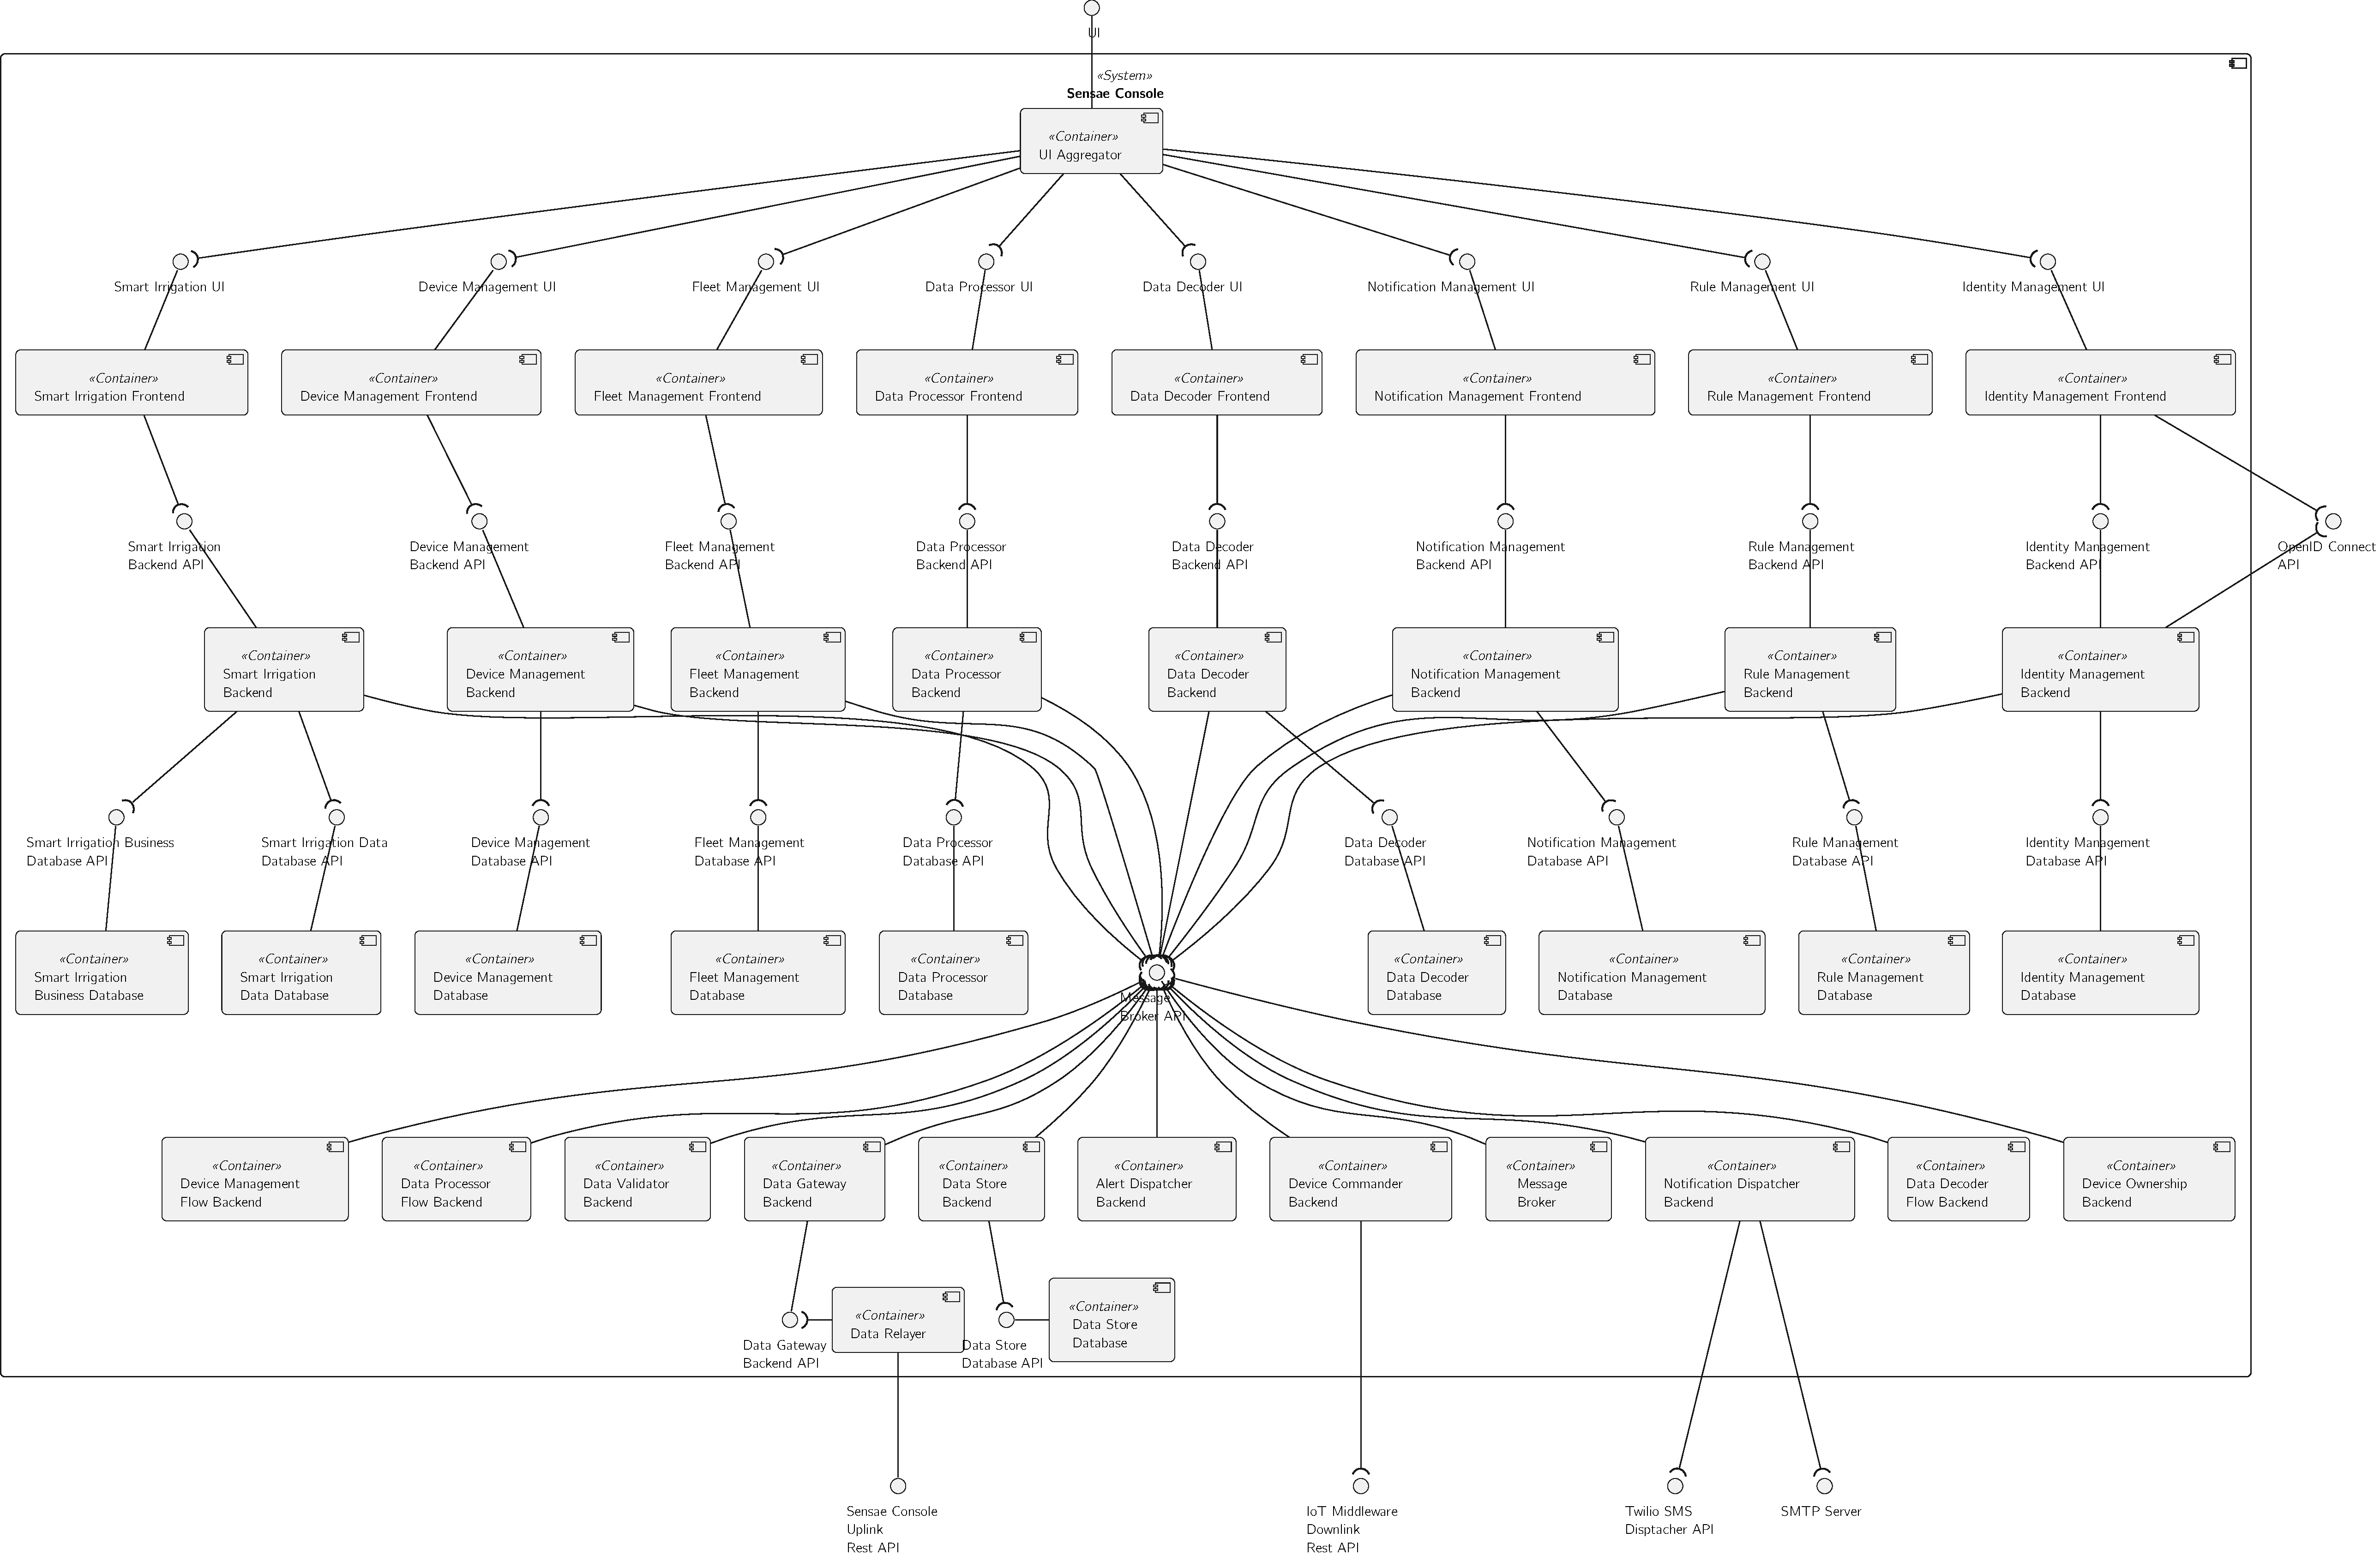
\includegraphics[page=1,width=0.8\columnwidth]{assets/diagrams/design/architectural/level2/logical/complete.pdf}
   \caption[Complete Solution - Container Level - Logical View Diagram]{Complete Solution - Container Level - Logical View Diagram}
   \label{fig:AppendixB:complete}
\end{sidewaysfigure}


\chapter{Platform Design - C4 Level 3 - Components}
\label{appendix:design:architecture:platform:components}

The component level describes the internals of a specific container. A container is made up of a number of components, each with well-defined responsibilities. In the following diagrams the dependencies between the various components will also be presented.

Most developed containers share the same architecture and will therefore be addressed as groups of containers.

The physical view will not be presented since all relevant details have been addressed above.

\section{Components Level - Logical View}
\label{par:design:architecture:platform:components:logical}

The architectures used in the various developed containers can be condensate into 3 types with minor variations:

\begin{itemize}
   \item \textbf{Frontend Architecture}: used on all Configuration scope frontend containers;
   \item \textbf{Configuration Backend Architecture}: used on all Configuration scope backend containers;
   \item \textbf{Data Flow Architecture}: used on most Data Flow scope containers.
\end{itemize}

Starting with the Frontend Architecture used, it was decided to maintain two distinct domains (Model and DTOS) in order to meet the \gls{SRP} (high cohesion) and to lower the coupling between the information displayed in the UI and the data sent/received by the container. This segmentation led to the addition of the Mapper component, which has the responsibility of converting the data (DTOS component) into information (Model component) and vice-versa. The Auth component indicates what backend resources the user has access to, by decoding the \textit{access token}, and the Utils component has several methods commonly used to process backend requests. These two components are reused in all frontend containers, including the ones related to the External Services.

As an example, the logical view of the Data Decoder Frontend is presented in Figure~\ref{fig:design:architecture:platform:component:logical:diagram:decoder}.

\begin{figure}[H]
   \centering
   \resizebox{0.7\columnwidth}{!}
   {
      \input{assets/diagrams/design/architectural/level3/logical/data-decoder-frontend.latex}
   }
   \caption[Component Level - Data Decoder Frontend - Logical View Diagram]{Component Level - Data Decoder Frontend - Logical View Diagram}
   \label{fig:design:architecture:platform:component:logical:diagram:decoder}
\end{figure}

This architecture is used on the containers: (i) Device Management Frontend, (ii) Data Decoder Frontend, (iii) Data Processor Frontend, (iv) Rule Management Frontend. The UI Aggregator has a simpler architecture them the other frontend containers, it is comprised by a Presentation component that depends on the Auth component to handle user authentication and authorization.

Next, the Configuration Backend Architecture is discussed. It is based on the Onion Architecture, an architecture pattern that ``emphasizes separation of concerns throughout the system'' and ``leads to more maintainable applications'' \parencite{onion}.

As an example the logical view of the Device Management Backend is presented in Figure~\ref{fig:design:architecture:platform:component:logical:diagram:device}.

% \begin{figure}[H]
%    \centering
%    \resizebox{0.8\columnwidth}{!}
%    {
%       \input{assets/diagrams/design/architectural/level3/logical/device-management-backend.latex}
%    }
%    \caption[Component Level - Device Management Backend - Logical View Diagram]{Component Level - Device Management Backend - Logical View Diagram}
%    \label{fig:design:architecture:platform:component:logical:diagram:device}
% \end{figure}

This architecture is used on the containers: (i) Device Management Backend, (ii) Data Decoder Backend, (iii) Data Processor Backend, (iv) Rule Management Backend, (v) Identity Management Backend.

The following table, Table~\ref{tab:design:architecture:platform:components:logical:backend}, discusses each component responsibilities.

\begin{table}[H]
   \centering
   \caption{Configuration Backend components responsibilities}
   \label{tab:design:architecture:platform:components:logical:backend}
   \begin{tabular}{@{}cl@{}}
   \toprule
   \textbf{Component}               & \textbf{Responsibilities}                                            \\ \midrule
   Infrastructure &
     \begin{tabular}[c]{@{}l@{}}- Enclose components that manage the Input/Output\\ operations required by the container.\end{tabular} \\ \midrule
   Endpoint &
     \begin{tabular}[c]{@{}l@{}}- Enclose components that are used by external\\ containers to interact with the container.\end{tabular} \\ \midrule
   \multirow{2}{*}{AMQP} &
     - Define how to consume and publish events in the Message Broker; \\
    &
     \begin{tabular}[c]{@{}l@{}}- Delegate the handling of events received to \\ specific Application processes.\end{tabular} \\ \midrule
   \multirow{2}{*}{GraphQl}         &
     \begin{tabular}[c]{@{}l@{}} - Define the interface to be consumed by the \\ frontend and external Systems;  \end{tabular} \\
                                    & - Delegate external requests made to specific Application processes.\\ \midrule
   Persistence &
     \begin{tabular}[c]{@{}l@{}}- Enclose components that interface with \\ containers responsible for persisting data.\end{tabular} \\ \midrule
   Postgres                         & - Interact with a database to persist and query data.                \\ \midrule
   \multirow{4}{*}{Application}     & - Represent the application processes;                               \\
    &
     \begin{tabular}[c]{@{}l@{}}- Ensure the propagation of events related to the\\ process in question, requiring this responsibility to AMQP;\end{tabular} \\
    &
     \begin{tabular}[c]{@{}l@{}}- Ensure the execution of the process in question,\\ requiring this responsibility to Domain Services;\end{tabular} \\
                                    & - Enforce user authorization.                                        \\ \midrule
   \multirow{3}{*}{Domain Services} & - Represent business processes;                                      \\
                                    & - Interact with the Domain;                                  \\
    &
     \begin{tabular}[c]{@{}l@{}}- Ensure the persistence of the data in question,\\ requiring this responsibility to the Persistence.\end{tabular} \\ \midrule
   \multirow{2}{*}{Domain}          & - Represent de business rules and concepts;                          \\
                                    & - Manage the system information.                                    \\ \bottomrule
   \end{tabular}
\end{table}

Finally the architecture used in containers related to the Data Flow Scope is presented. It is based on a simplified version of the Onion Architecture since the intrinsic processes of these containers are much simpler.

As an example the logical view of the Device Ownership Backend is presented in Figure~\ref{fig:design:architecture:platform:component:logical:diagram:ownership}.

% \begin{figure}[H]
%    \centering
%    \resizebox{\columnwidth}{!}
%    {
%       \input{assets/diagrams/design/architectural/level3/logical/device-ownership-backend.latex}
%    }
%    \caption[Component Level - Device Ownership Backend - Logical View Diagram]{Component Level - Device Ownership Backend - Logical View Diagram}
%    \label{fig:design:architecture:platform:component:logical:diagram:ownership}
% \end{figure}

This architecture is used on the containers: (i) Device Management Flow Backend, (ii) Data Decoder Flow Backend, (iii) Data Processor Flow Backend, (iv) Device Ownership Backend. The responsibilities of the components inside AMQP are:

\begin{itemize}
   \item Internal: responsible for communicating with the system via internal topic;
   \item Ingress: responsible for consuming events/messages coming from data, alert or command topics;
   \item Egress: responsible for publishing events/messages to the data or alert topics.
\end{itemize}

The Memory component is responsible for caching unhandled data units and other information relevant for each context. This component is not present in Data Validator Backend and Alert Dispatcher Backend since they don't need to store context information to function.

The Data Gateway, Device Commander and Data Store backend containers have architectures that derive from this one and can be consulted in Appendix ~\ref{AppendixC}.

\section{Components Level - Process View}
\label{par:design:architecture:platform:components:process}

In this section some internal process deemed relevant are presented through sequence diagrams in order to familiarize the reader with the interactions that occur between components inside a container.

The internal processes that will be evaluated are:

\begin{itemize}
   \item Process Data Unit in Device Management Flow Backend;
   \item Deploy Draft Rule Scenarios in Rule Management Backend.
\end{itemize}

This processes have been chosen in order to introduce the reader to specific operations not yet explored in this chapter.

The first process to explore is meant to clarify how a Data Unit sent by a Controller (devices that collect and report measures of various sensors) is processed inside the Device Management Flow Backend. As explained in the \nameref{subsubsec:design:domain:bounded_contexts:device} Section, Data Units sent by a Controller are partitioned into various Data Units. The following diagram, Figure~\ref{fig:design:architecture:platform:component:process:diagram:device}, details this process.

\begin{figure}[H]
   \centering
   \resizebox{\columnwidth}{!}
   {
      \input{assets/diagrams/design/architectural/level3/process/device-management-flow-backend.latex}
   }
   \caption[Component Level - Process Data Unit in Device Management Flow Backend - Process View Diagram]{Component Level - Process Data Unit in Device Management Flow Backend - Process View Diagram}
   \label{fig:design:architecture:platform:component:process:diagram:device}
\end{figure}

As presented in the diagram:

\begin{itemize}
   \item As soon as the message dto arrives, it is mapped to the \textit{iot-core} data unit model - step \textbf{2} - this model is used inside every Data Flow container. Before publishing the data unit it is mapped to the dto once again - step \textbf{15} and \textbf{22}. This conversion happens with any other event published and consumed in the system;
   \item If the device information is found, a \textit{ping} notification for that device is sent - steps \textbf{6} to \textbf{8}, otherwise an \textit{unknown} notification would be sent and the container would store the data unit in the Memory component and process it when possible;
   \item For each sub device of the controller, a new data unit with that device measures is published in the system - steps \textbf{19} to \textbf{23};
\end{itemize}

Next, the process of deploying draft rule scenarios is described.
Draft scenarios exist since adding, removing or changing a rule scenario in Alert Dispatcher Backend requires the entire data set to be removed. This procedure can lead to alerts not being dispatched. The next diagram, Figure~\ref{fig:design:architecture:platform:component:process:diagram:rule}, tackles this concern.

% \begin{figure}[H]
%    \centering
%    \resizebox{\columnwidth}{!}
%    {
%       \input{assets/diagrams/design/architectural/level3/process/rule-management-backend.latex}
%    }
%    \caption[Component Level - Deploy Draft Rule Scenarios in Rule Management Backend - Process View Diagram]{Component Level - Deploy Draft Rule Scenarios in Rule Management Backend - Process View Diagram}
%    \label{fig:design:architecture:platform:component:process:diagram:rule}
% \end{figure}

As seen in the diagram, to mitigate the number of lost alerts, new rule scenarios are published at best every 30 minutes - step \textbf{1} - and only if any change was made - step \textbf{17} and \textbf{18}.

\section{Components Level - Implementation View}
\label{par:design:architecture:platform:components:development}

The implementation view of each container can also be condensate in the same 3 distinct types presented in the Section \nameref{par:design:architecture:platform:components:logical}.

The next diagrams, Figure~\ref{fig:design:architecture:platform:component:development:diagram:decoder}, Figure~\ref{fig:design:architecture:platform:component:development:diagram:device} and Figure~\ref{fig:design:architecture:platform:component:development:diagram:ownership} describe this view at the components level.

% \begin{figure}[H]
%    \centering
%    \resizebox{\columnwidth}{!}
%    {
%       \input{assets/diagrams/design/architectural/level3/development/data-decoder-frontend.latex}
%    }
%    \caption[Component Level - Data Decoder Frontend - Implementation View Diagram]{Component Level - Data Decoder Frontend - Implementation View Diagram}
%    \label{fig:design:architecture:platform:component:development:diagram:decoder}
% \end{figure}

The packages presented correspond to the components described in the logical view (Figure~\ref{fig:design:architecture:platform:component:logical:diagram:decoder}). Since the names given in both views are different, the following list maps the logical view into the implementation view:

\begin{itemize}
   \item \textit{components} package corresponds to the \textit{Presentation} component;
   \item \textit{auth} package corresponds to the \textit{Auth} component;
   \item \textit{core} package corresponds to the \textit{Utils} component;
   \item \textit{dtos} package corresponds to the \textit{DTOS} component;
   \item \textit{mappers} package corresponds to the \textit{Mappers} component;
   \item \textit{model} package corresponds to the \textit{Model} component;
   \item \textit{services} package corresponds to the \textit{Services} component.
\end{itemize}

% \begin{figure}[H]
%    \centering
%    \resizebox{0.8\columnwidth}{!}
%    {
%       \input{assets/diagrams/design/architectural/level3/development/device-management-backend.latex}
%    }
%    \caption[Component Level - Device Management Backend - Implementation View Diagram]{Component Level - Device Management Backend - Implementation View Diagram}
%    \label{fig:design:architecture:platform:component:development:diagram:device}
% \end{figure}

The packages presented correspond to the components described in the logical view (Figure~\ref{fig:design:architecture:platform:component:logical:diagram:device}). The names given in both views differ only on the case used.

\begin{figure}[H]
   \centering
   \resizebox{0.8\columnwidth}{!}
   {
      \input{assets/diagrams/design/architectural/level3/development/device-ownership-backend.latex}
   }
   \caption[Component Level - Device Ownership Backend - Implementation View Diagram]{Component Level - Device Ownership Backend - Implementation View Diagram}
   \label{fig:design:architecture:platform:component:development:diagram:ownership}
\end{figure}

The packages presented correspond to the components described in the logical view (Figure~\ref{fig:design:architecture:platform:component:logical:diagram:ownership}). The names given in both views differ only on the case used.

\chapter{Sensae Console - Components Level - Logical View}
\label{AppendixC}

This Appendix presents the logical view, component level, of the Data Flow scope containers that had minor differences when compared with the other containers.

\begin{figure}[H]
   \centering
   \resizebox{0.6\columnwidth}{!}
   {
      \input{assets/diagrams/design/architectural/level3/logical/data-gateway.latex}
   }
   \caption[Component Level - Data Gateway - Logical View Diagram]{Component Level - Data Gateway - Logical View Diagram}
   \label{fig:AppendixC:gateway}
\end{figure}

\begin{figure}[H]
   \centering
   \resizebox{0.6\columnwidth}{!}
   {
      \input{assets/diagrams/design/architectural/level3/logical/data-store.latex}
   }
   \caption[Component Level - Data Store - Logical View Diagram]{Component Level - Data Store - Logical View Diagram}
   \label{fig:AppendixC:store}
\end{figure}


\begin{figure}[H]
   \centering
   \resizebox{0.7\columnwidth}{!}
   {
      \input{assets/diagrams/design/architectural/level3/logical/device-commander.latex}
   }
   \caption[Component Level - Device Commander - Logical View Diagram]{Component Level - Device Commander - Logical View Diagram}
   \label{fig:AppendixC:commander}
\end{figure}

\chapter{External Services - Components Level - Logical View}
\label{AppendixC2}

This Appendix presents the logical view, component level, of all backend containers related to the \gls{PoC}s developed.

The \textit{AMQP API} is the one represented as \textit{Sensae API for External Services} in most logical diagrams.

\begin{figure}[H]
   \centering
   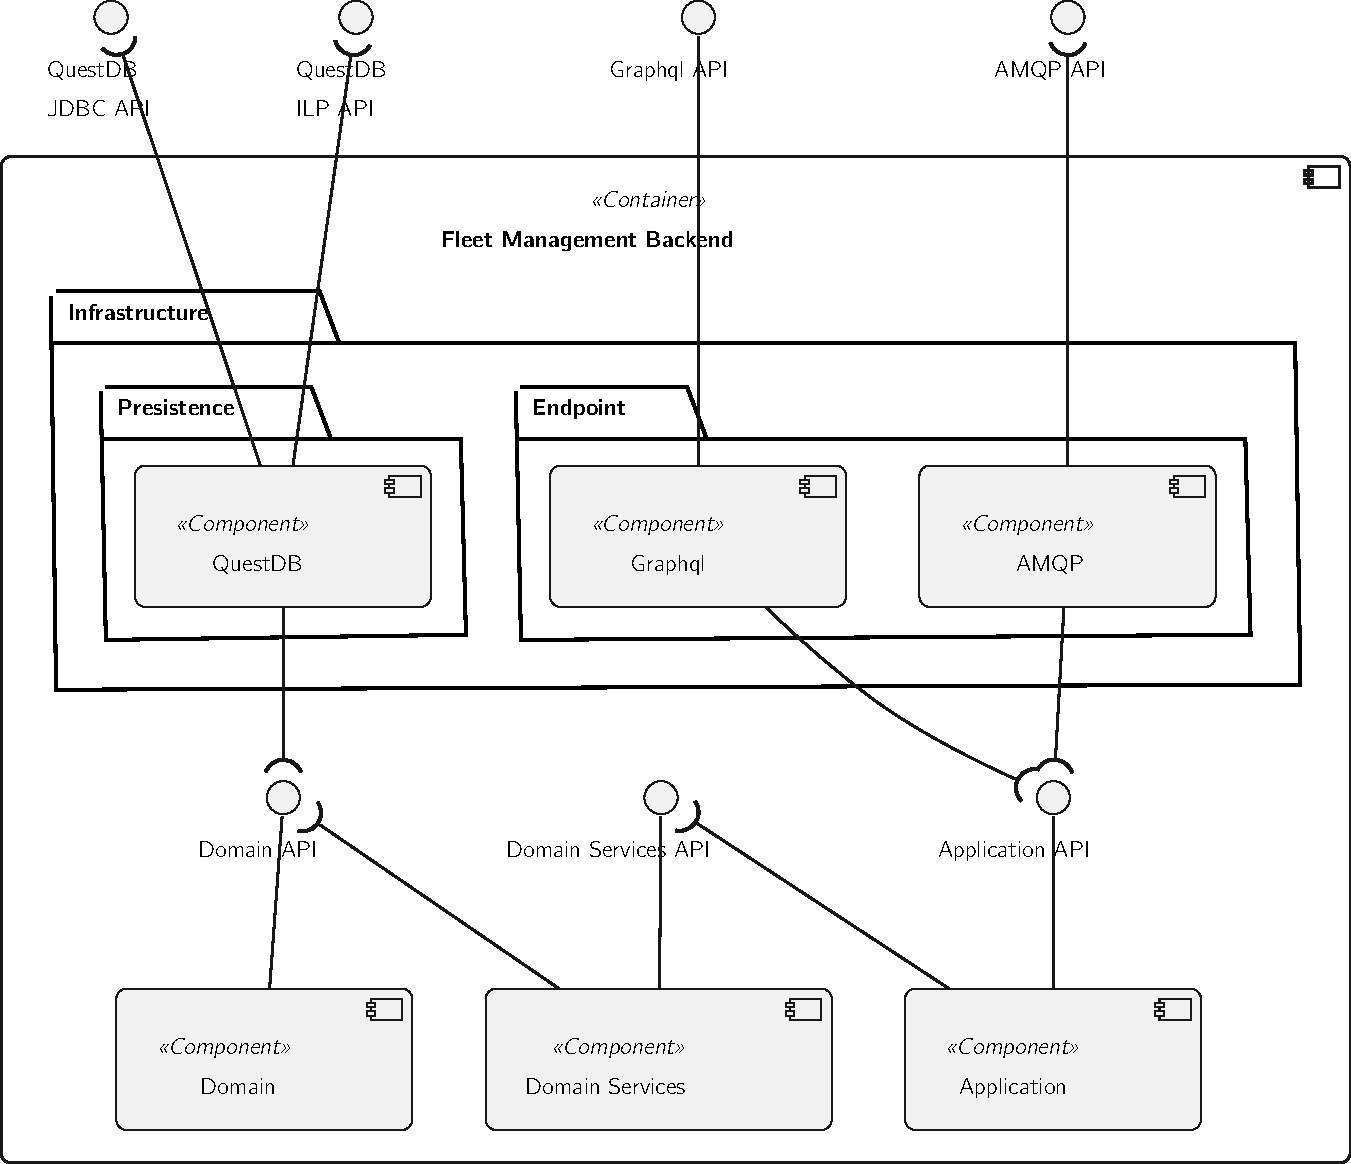
\includegraphics[page=1,width=0.8\columnwidth]{assets/diagrams/design/architectural/level3/logical/fleet-management-backend.pdf}
   \caption[Component Level - Fleet Management Backend - Logical View Diagram]{Component Level - Fleet Management Backend - Logical View Diagram}
   \label{fig:AppendixC2:fleet}
\end{figure}

\begin{figure}[H]
   \centering
   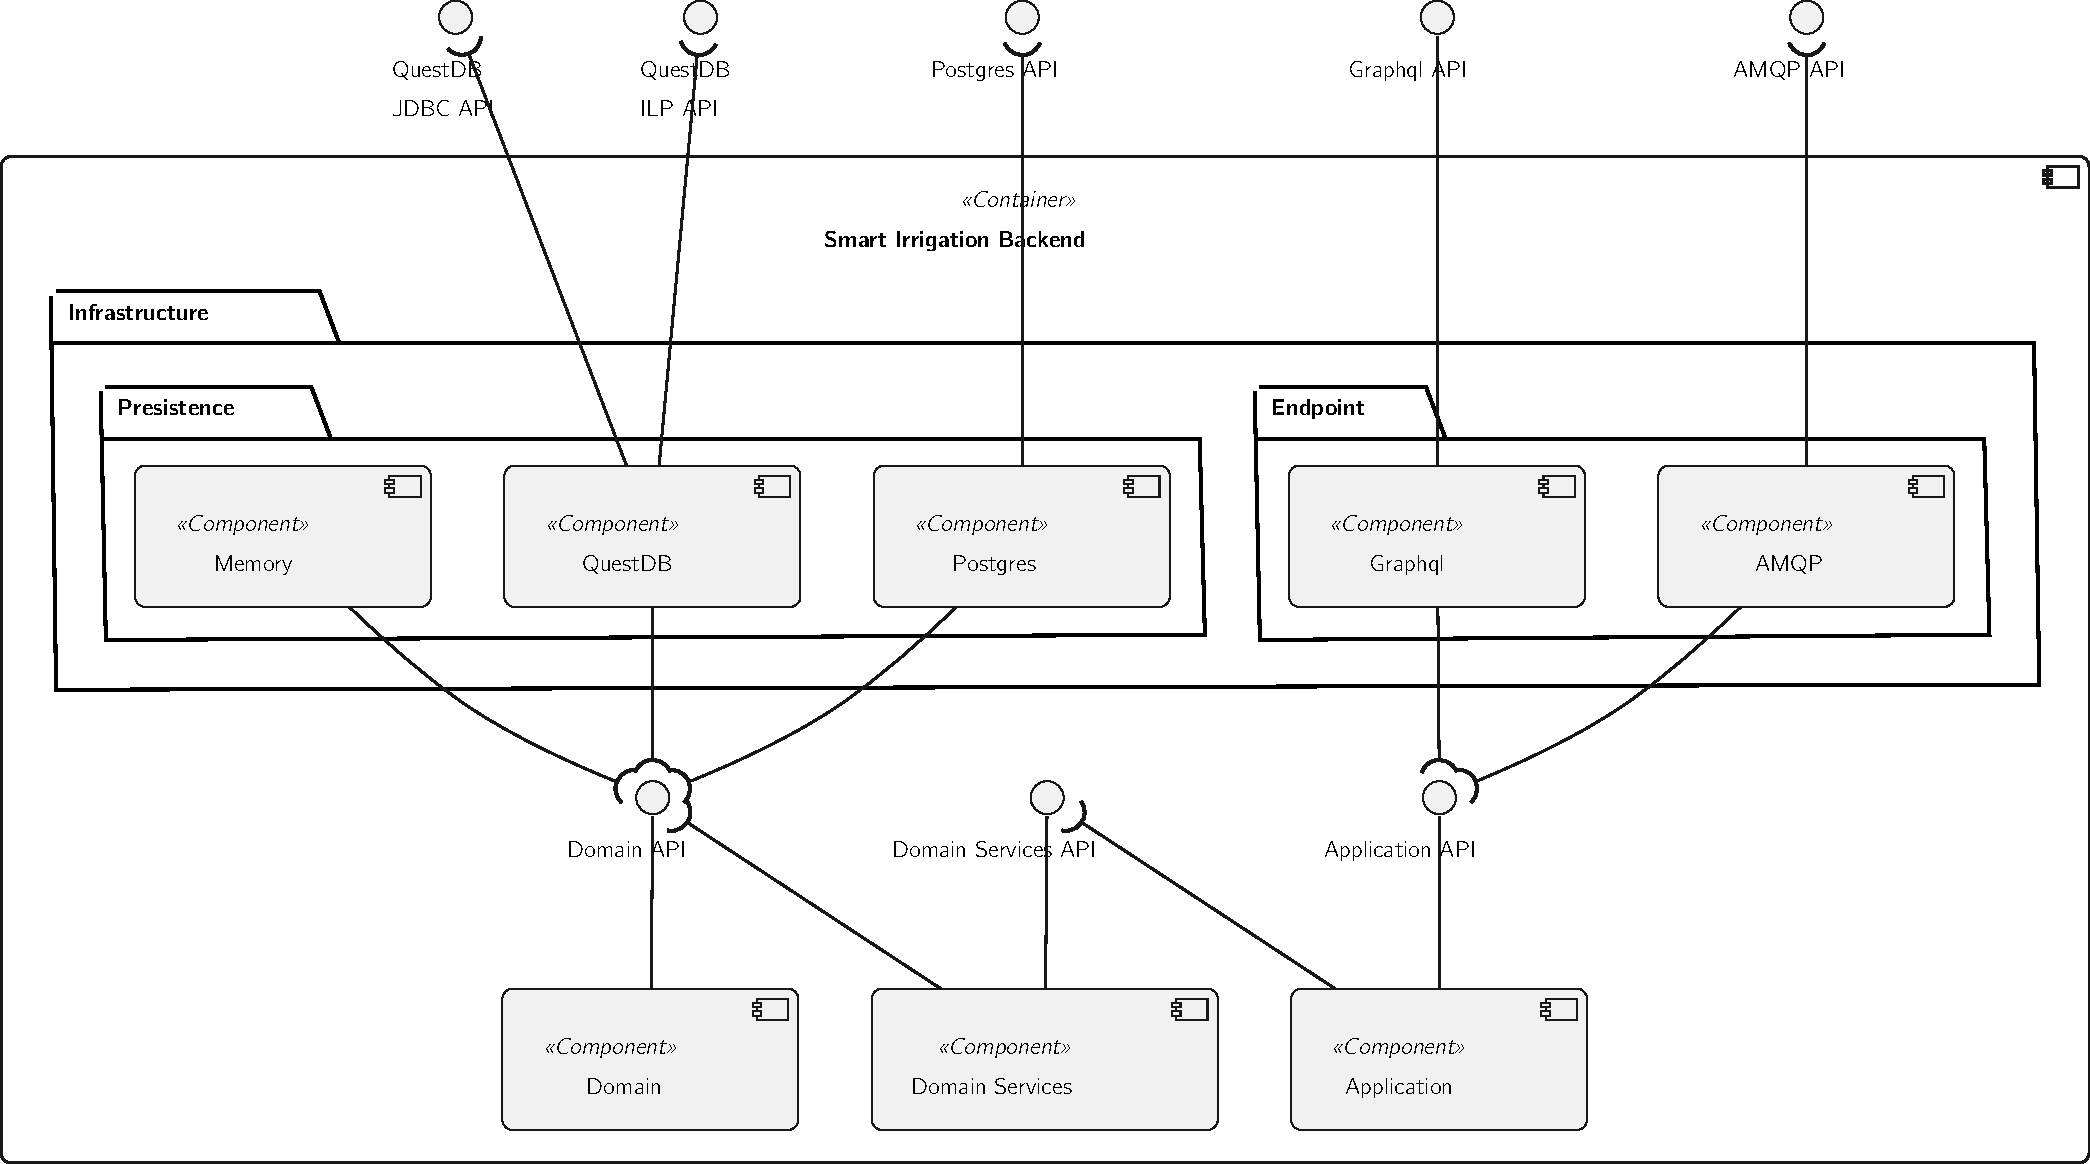
\includegraphics[page=1,width=\columnwidth]{assets/diagrams/design/architectural/level3/logical/smart-irrigation-backend.pdf}
   \caption[Component Level - Smart Irrigation Backend - Logical View Diagram]{Component Level - Smart Irrigation Backend - Logical View Diagram}
   \label{fig:AppendixC2:irrig}
\end{figure}

\begin{figure}[H]
   \centering
   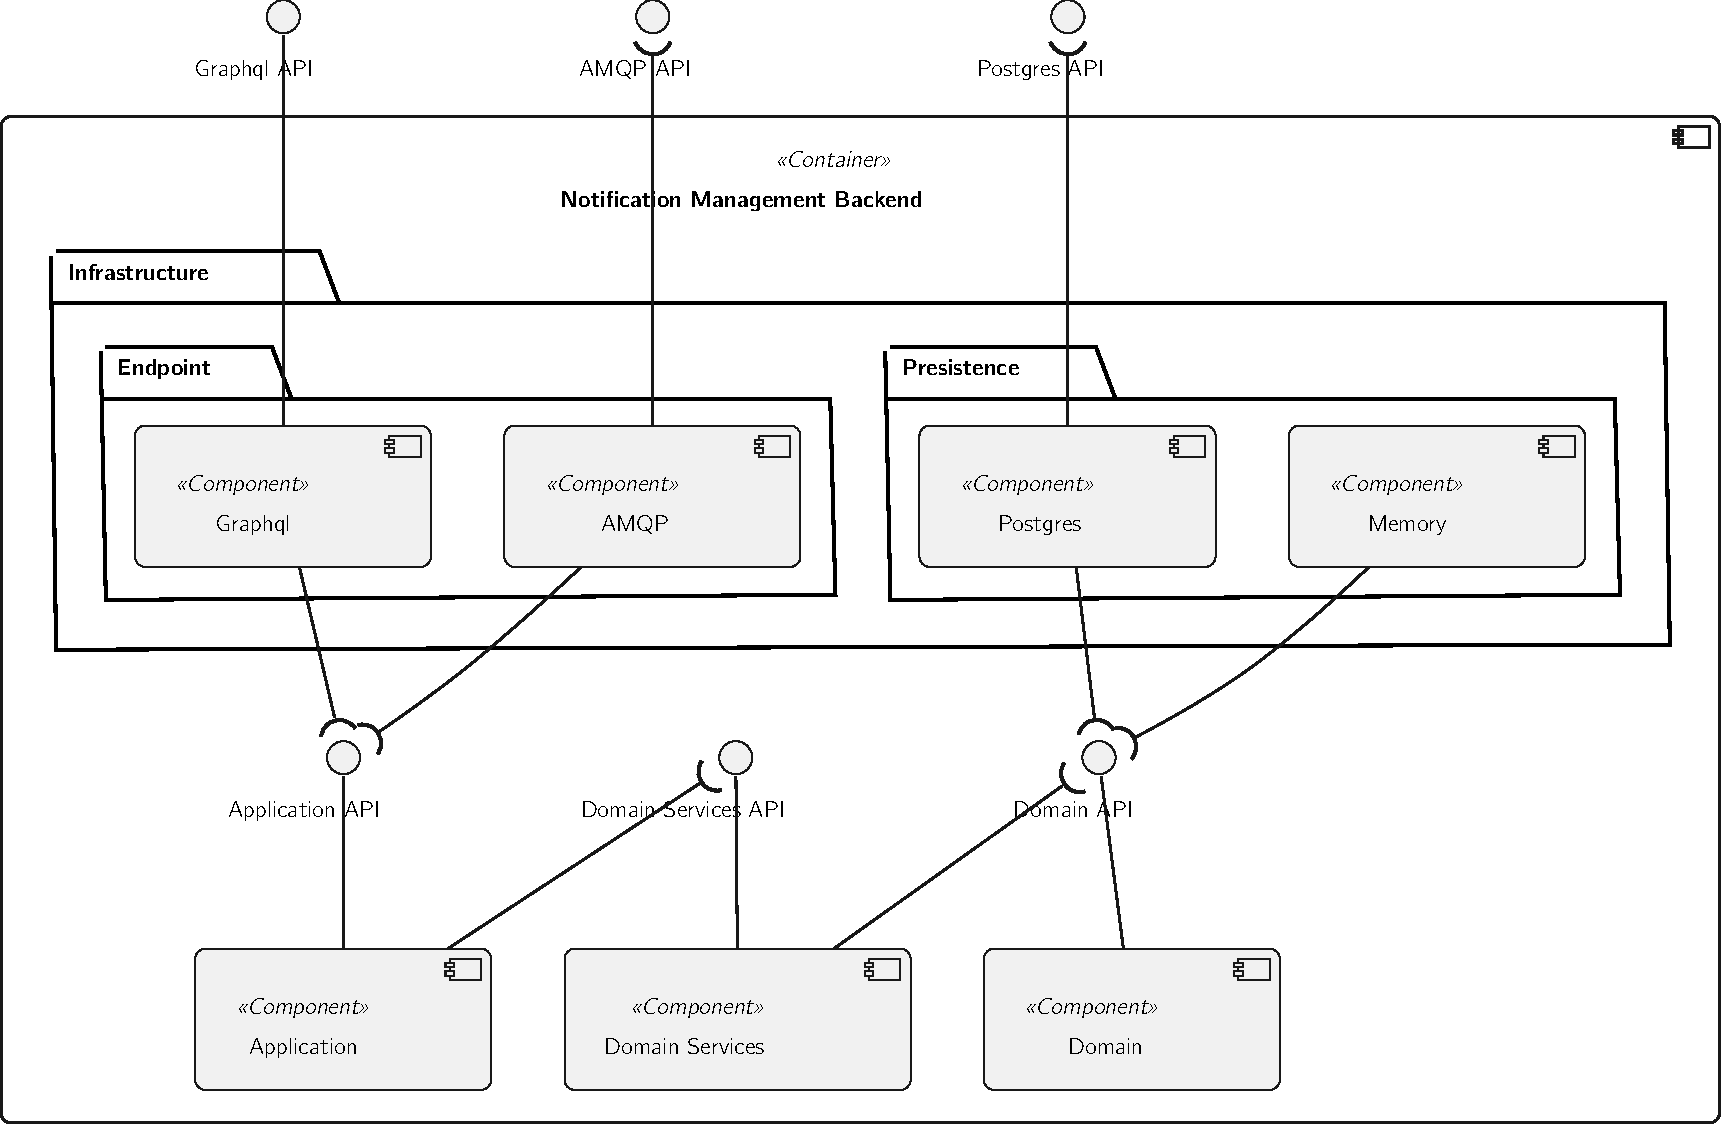
\includegraphics[page=1,width=\columnwidth]{assets/diagrams/design/architectural/level3/logical/notification-management-backend.pdf}
   \caption[Component Level - Notification Management Backend - Logical View Diagram]{Component Level - Notification Management Backend - Logical View Diagram}
   \label{fig:AppendixC2:noti}
\end{figure}

\begin{figure}[H]
   \centering
   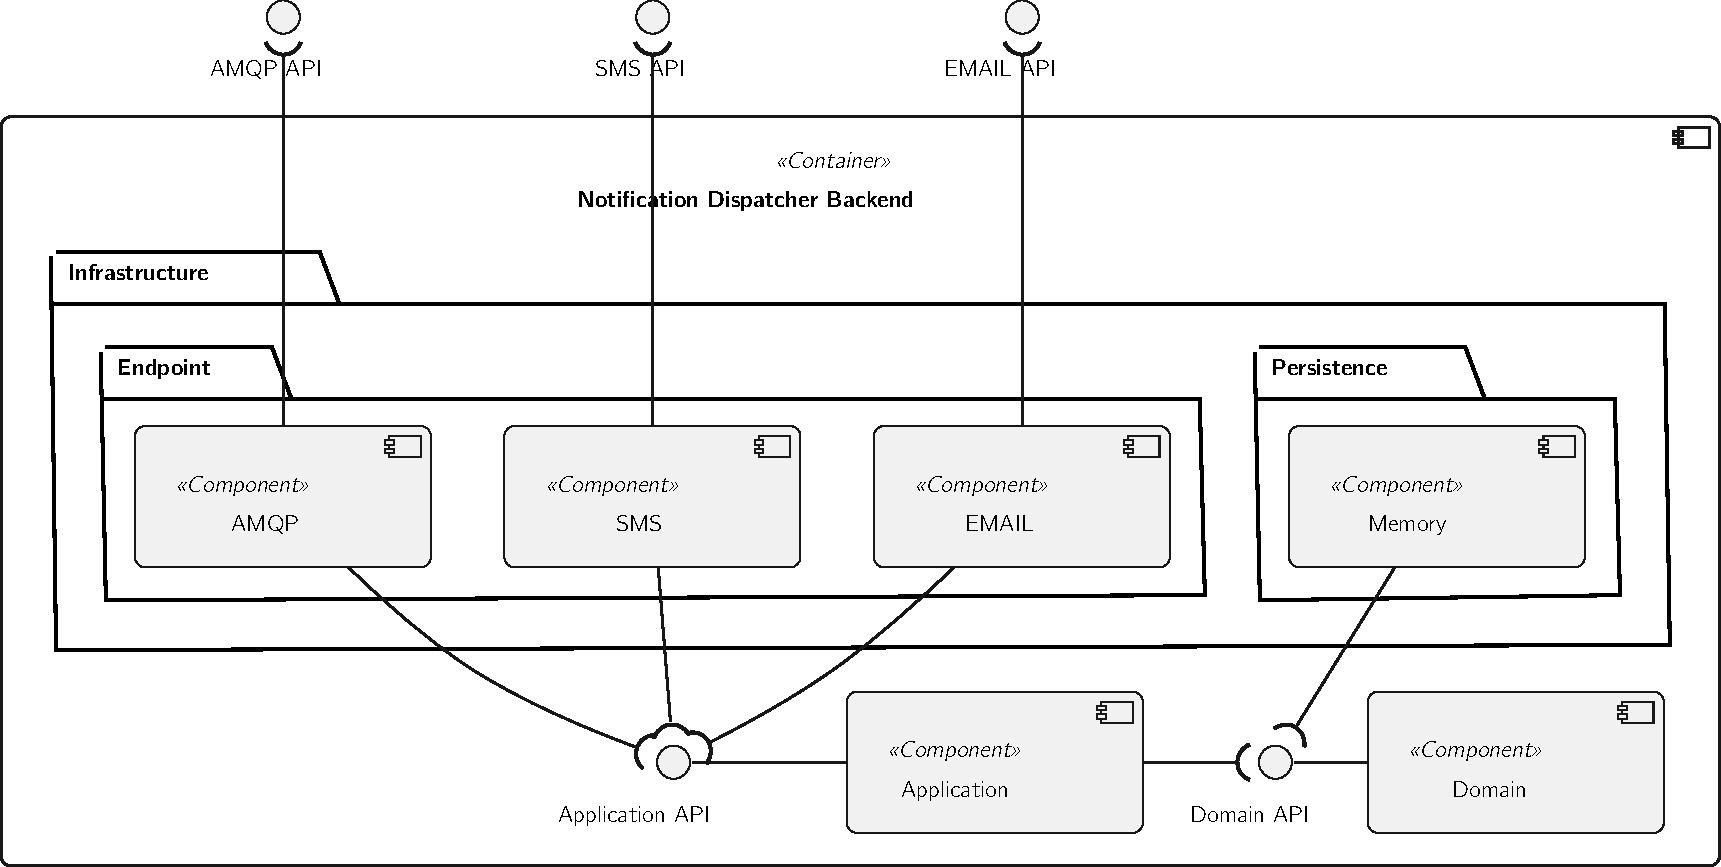
\includegraphics[page=1,width=\columnwidth]{assets/diagrams/design/architectural/level3/logical/notification-dispatcher-backend.pdf}
   \caption[Component Level - Notification Dispatcher Backend - Logical View Diagram]{Component Level - Notification Dispatcher Backend - Logical View Diagram}
   \label{fig:AppendixC2:notidispatcher}
\end{figure}

\chapter{Sensae Console - Additional UI Pages}
\label{AppendixD}

This appendix presents other \textbf{Sensae Console} pages.

\begin{figure}[H]
   \centering
   \resizebox{\columnwidth}{!}
   {
      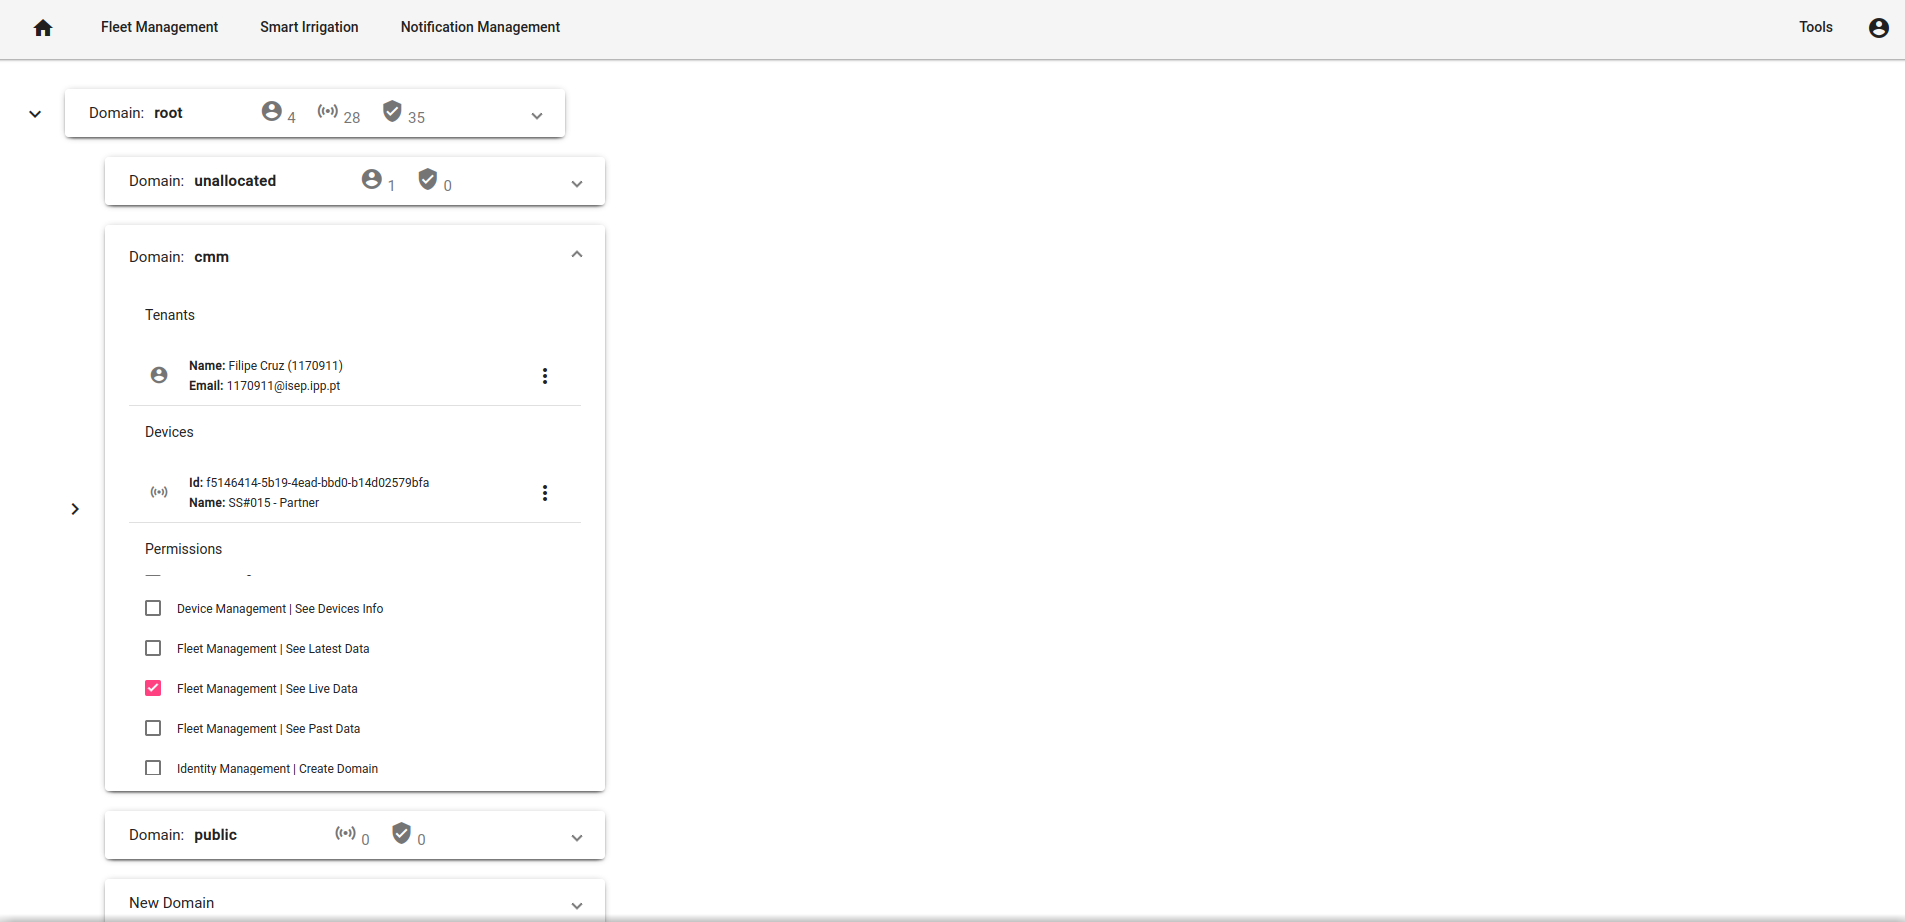
\includegraphics{assets/figures/ui/identity.png}
   }
   \caption[Identity Management Page]{Identity Management Page}
   \label{fig:AppendixD:identity}
\end{figure}

\begin{figure}[H]
   \centering
   \resizebox{\columnwidth}{!}
   {
      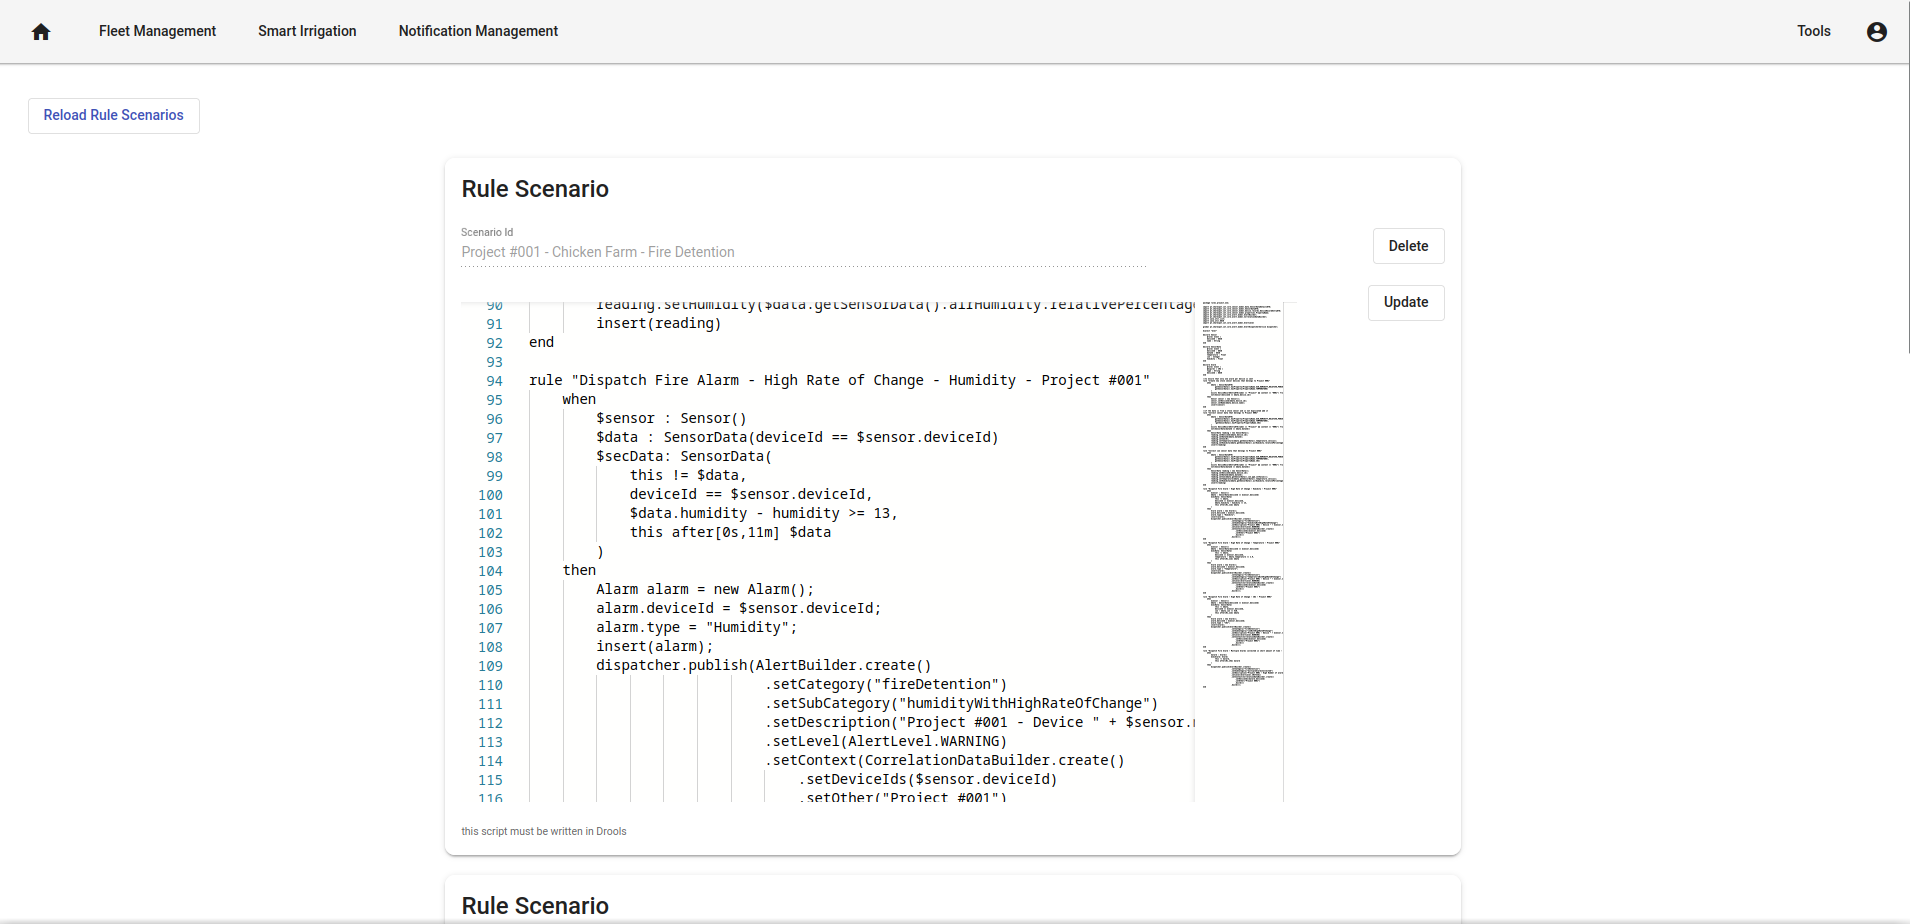
\includegraphics{assets/figures/ui/rules.png}
   }
   \caption[Rules Management Page]{Rules Management Page}
   \label{fig:AppendixD:rules}
\end{figure}

\begin{figure}[H]
   \centering
   \resizebox{\columnwidth}{!}
   {
      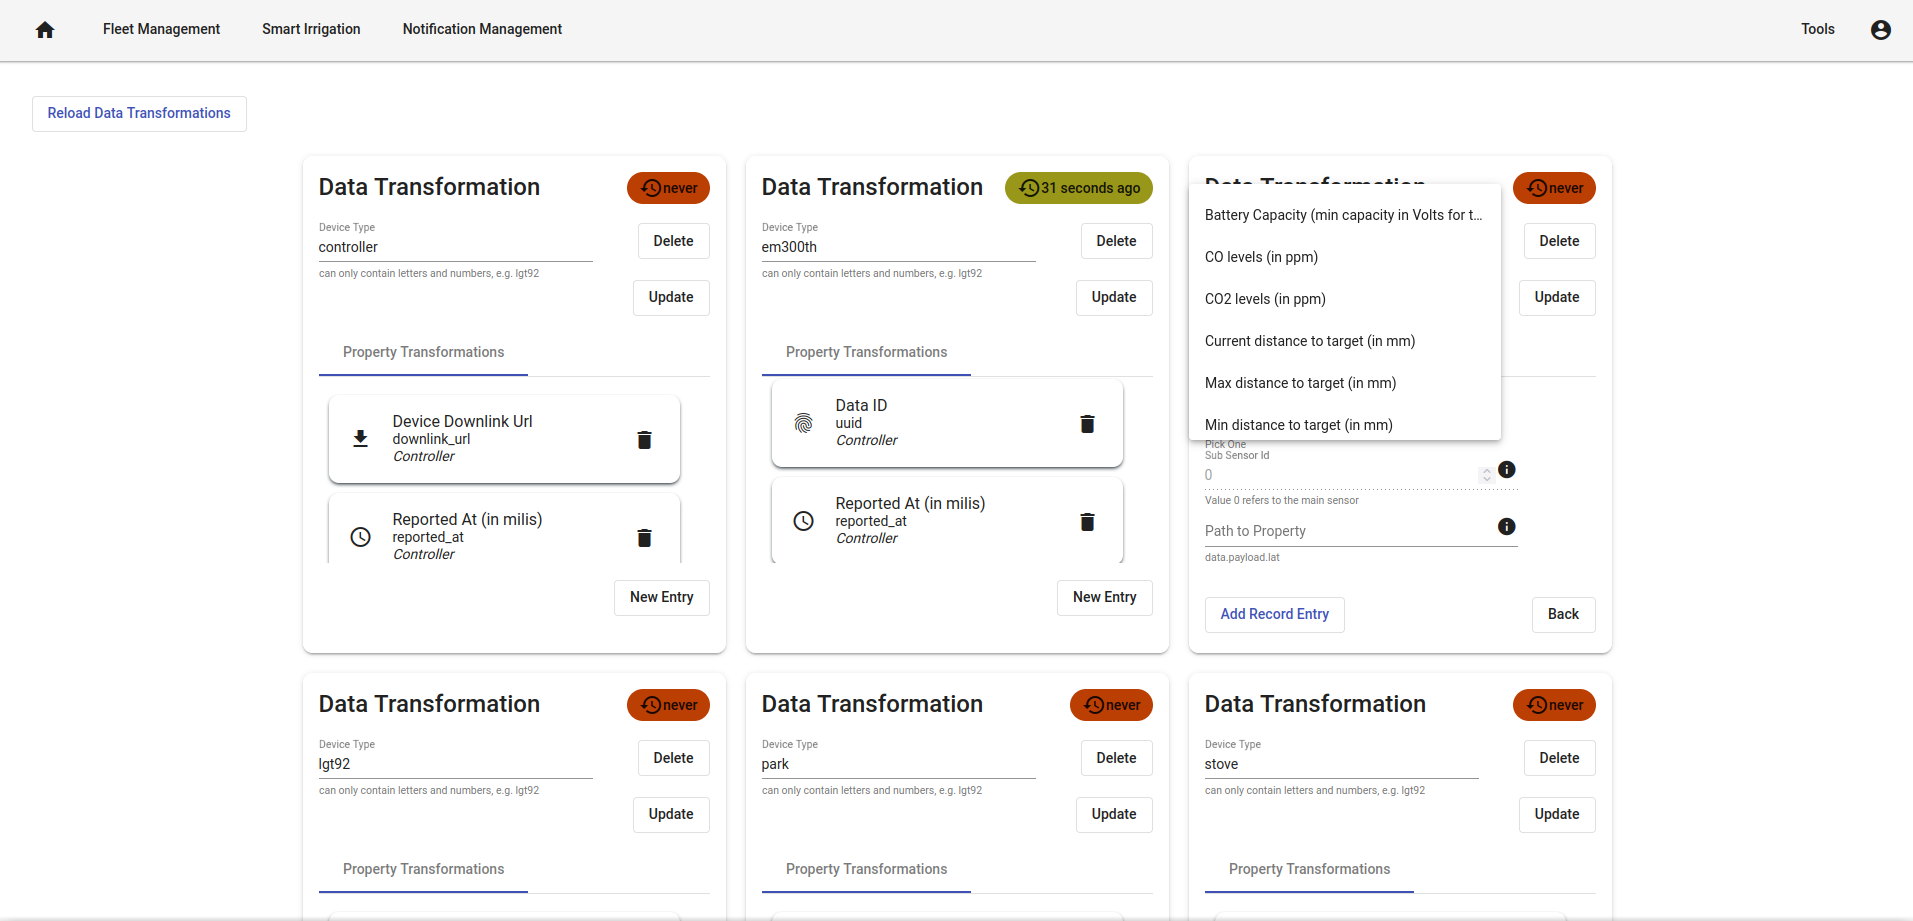
\includegraphics{assets/figures/ui/processor.png}
   }
   \caption[Data Processor Page]{Data Processor Page}
   \label{fig:AppendixD:processor}
\end{figure}

\begin{figure}[H]
   \centering
   \resizebox{\columnwidth}{!}
   {
      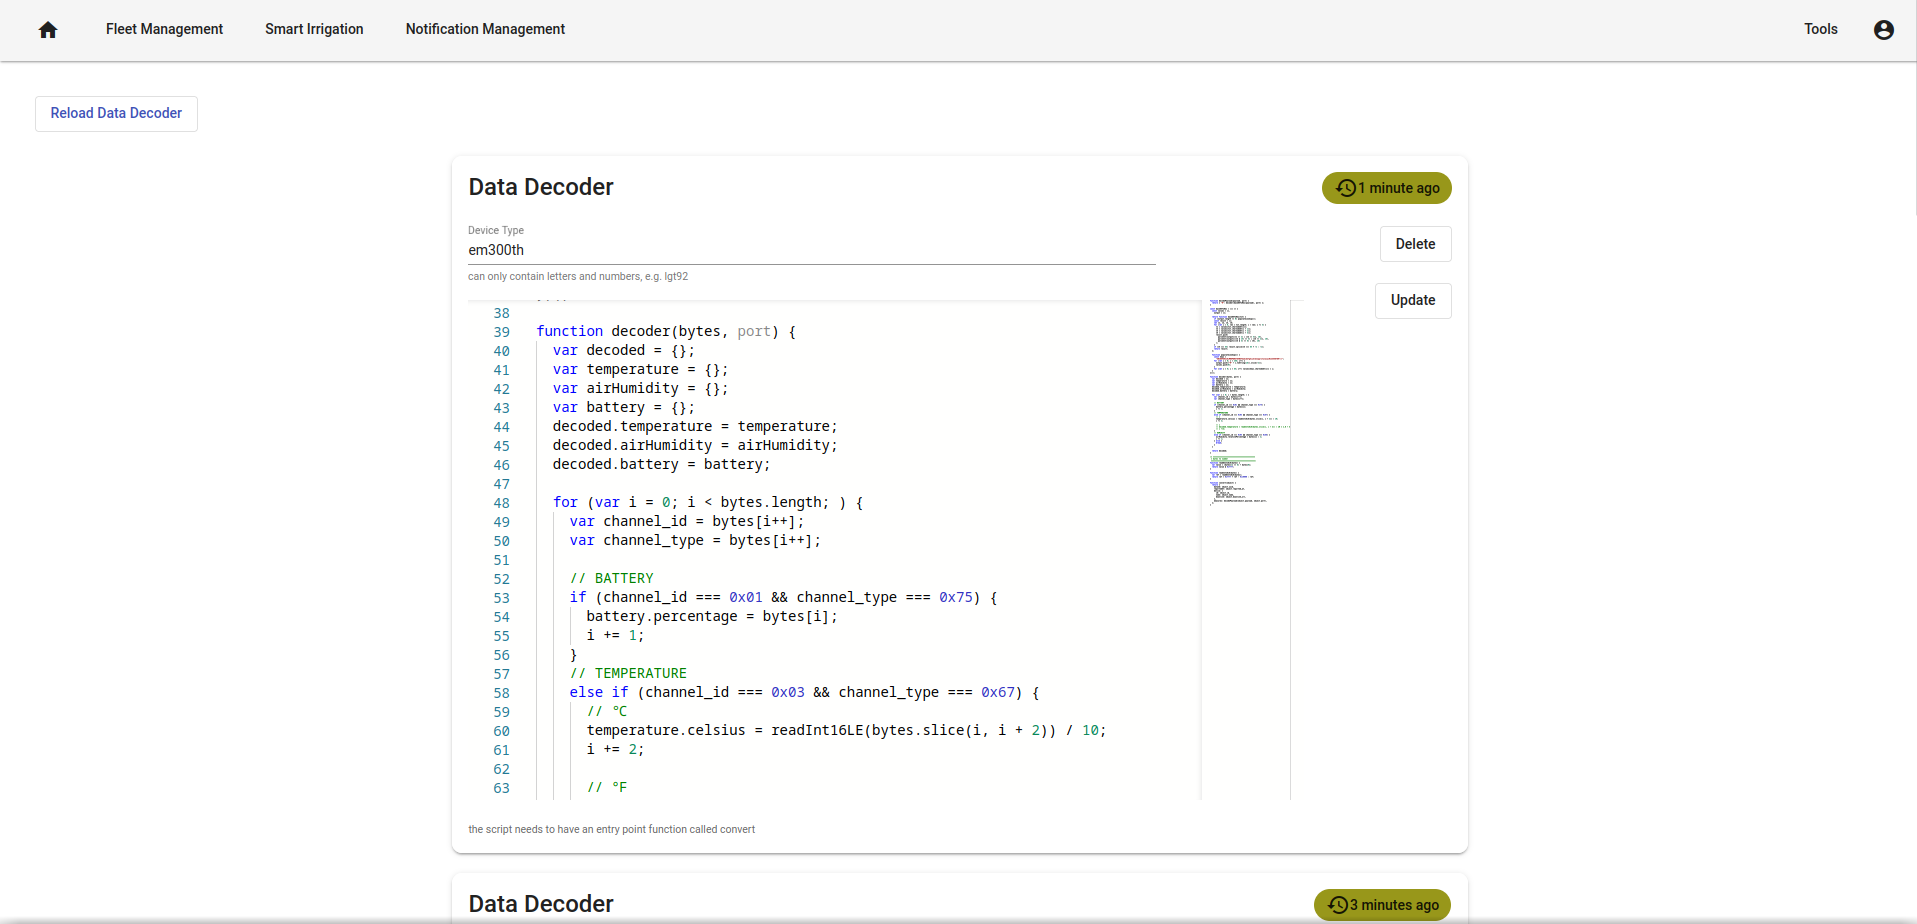
\includegraphics{assets/figures/ui/decoder.png}
   }
   \caption[Data Processor Page]{Data Decoder Page}
   \label{fig:AppendixD:decoder}
\end{figure}

\chapter{Solutions - Additional UI Pages}
\label{AppendixD2}

This appendix presents more pages related to the Solutions developed.

\begin{figure}[H]
   \centering
   \resizebox{\columnwidth}{!}
   {
      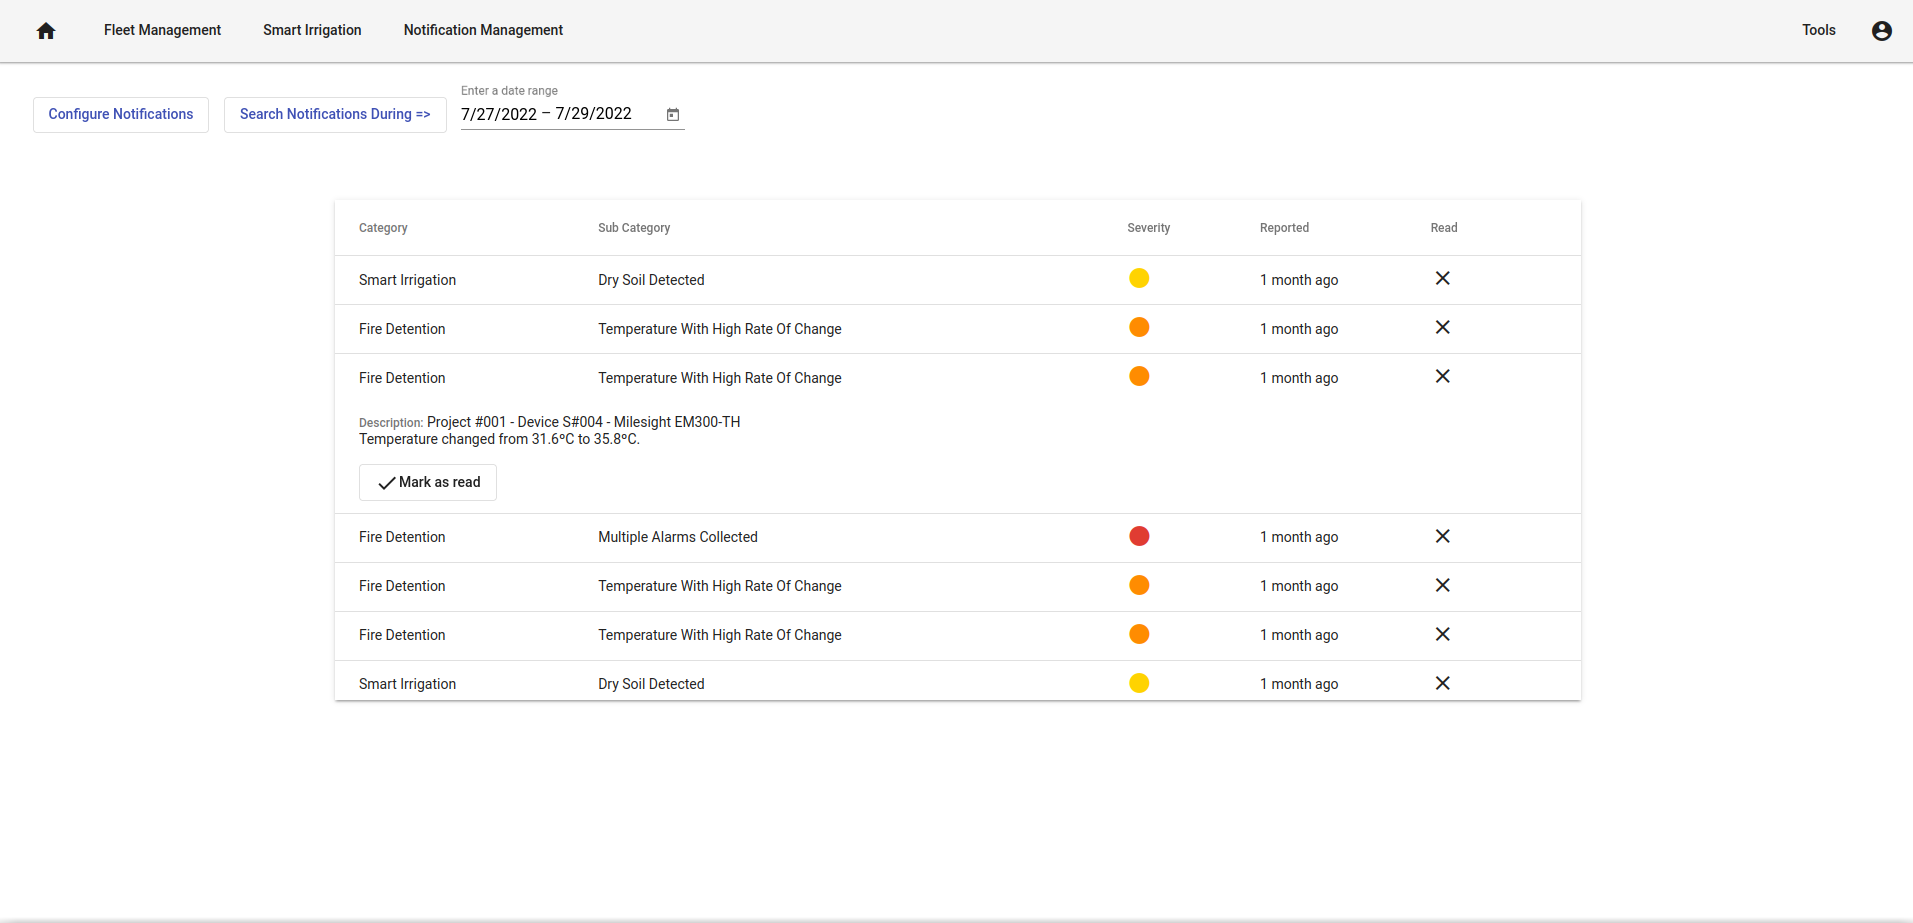
\includegraphics{assets/figures/ui/notification.png}
   }
   \caption[Notification Management Page]{Notification Management Page}
   \label{fig:AppendixD2:notification}
\end{figure}

\begin{figure}[H]
   \centering
   \resizebox{\columnwidth}{!}
   {
      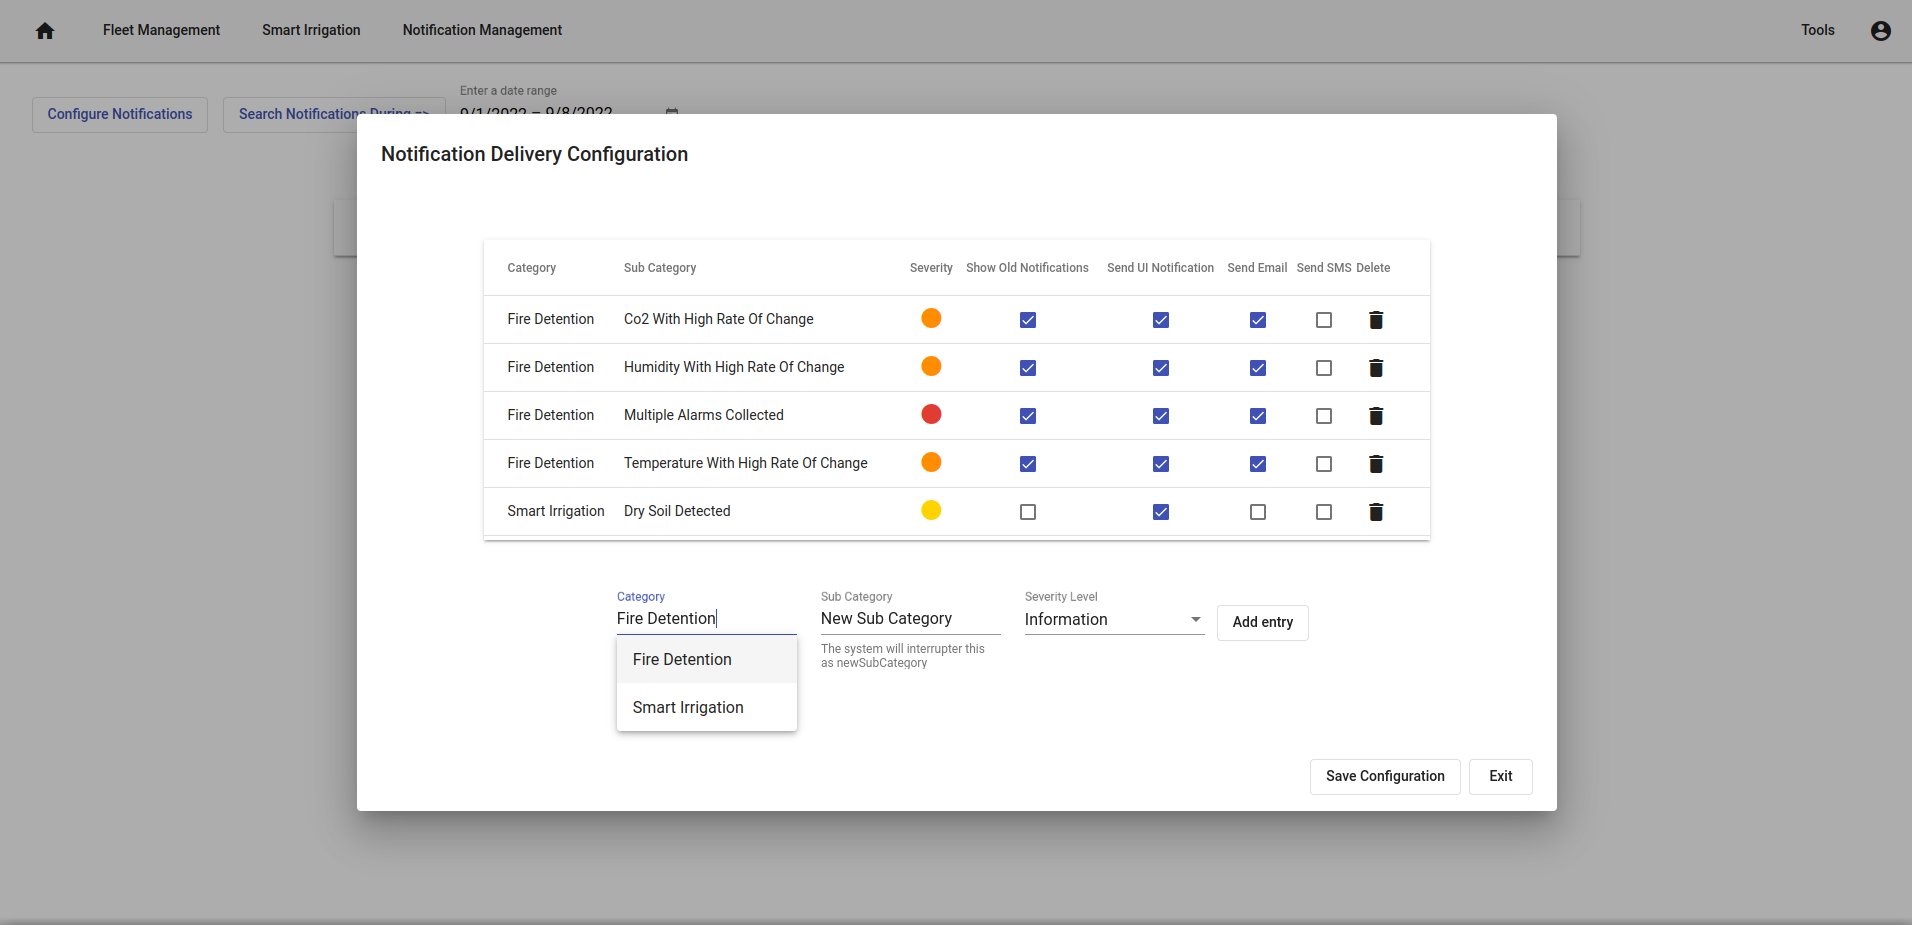
\includegraphics{assets/figures/ui/notification-configuration.png}
   }
   \caption[Notification Management Page - Configuration]{Notification Management Page - Configuration}
   \label{fig:AppendixD2:notificationconfig}
\end{figure}

\begin{figure}[H]
   \centering
   \resizebox{\columnwidth}{!}
   {
      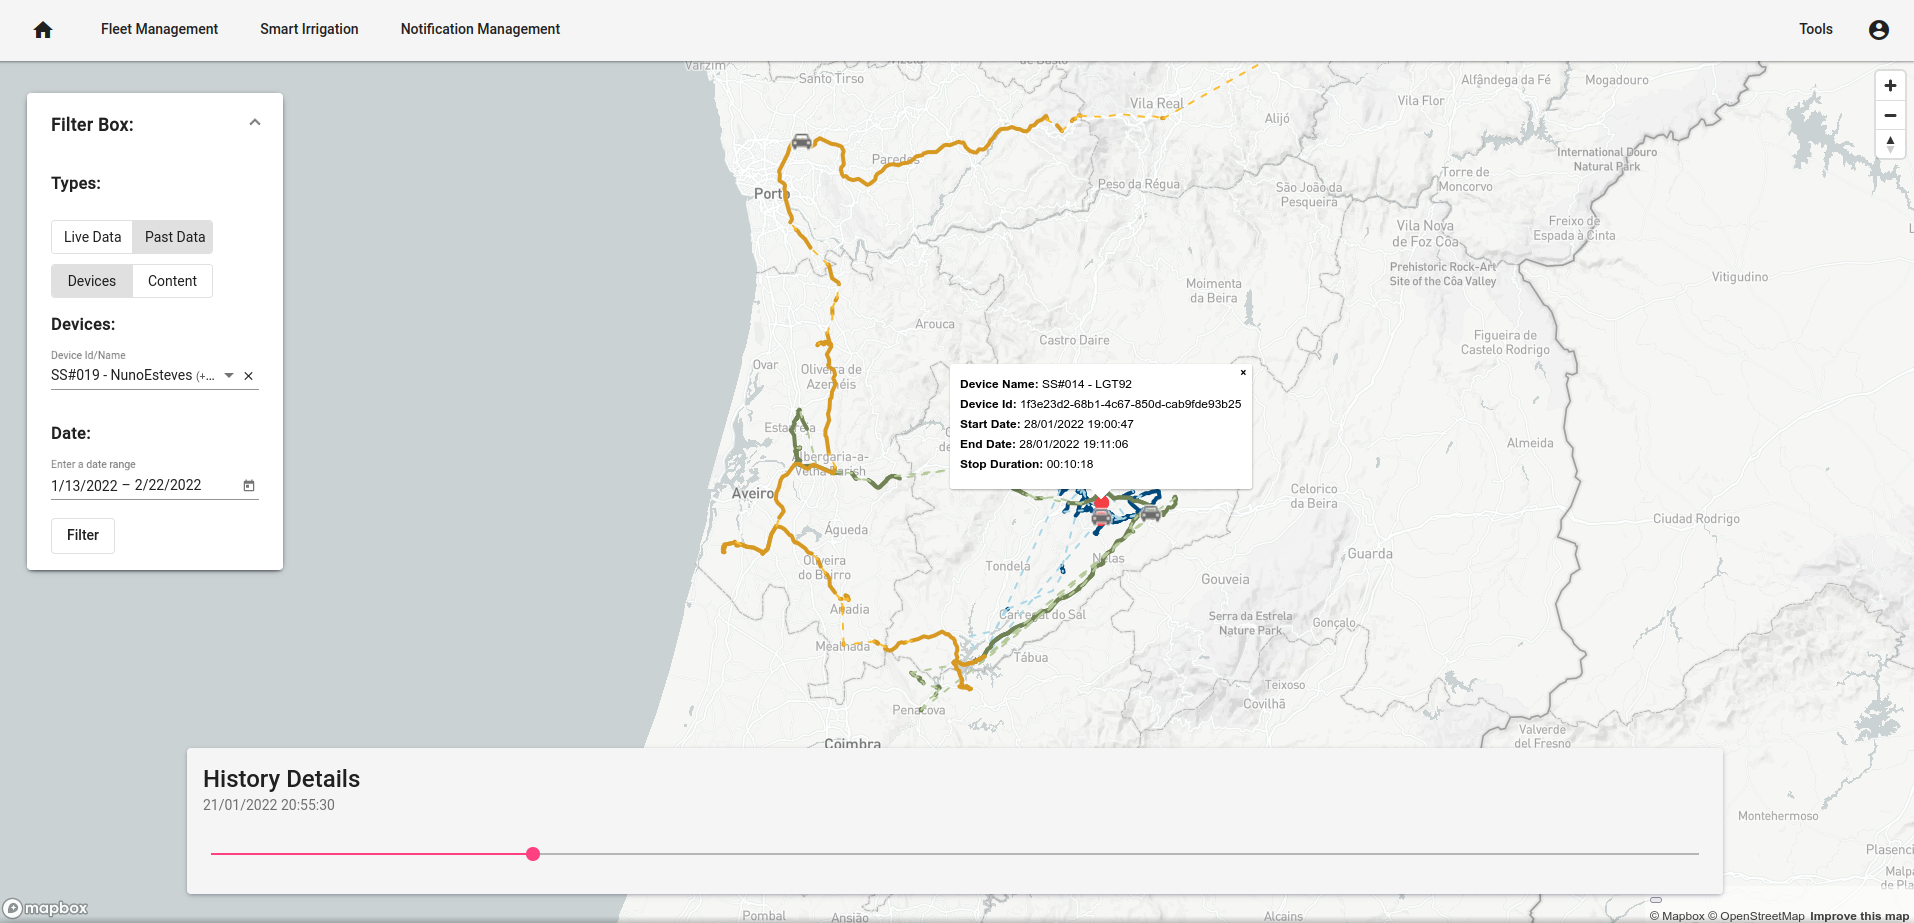
\includegraphics{assets/figures/ui/fleet.png}
   }
   \caption[Fleet Management Page]{Fleet Management Page}
   \label{fig:AppendixD2:fleet}
\end{figure}

\begin{figure}[H]
   \centering
   \resizebox{\columnwidth}{!}
   {
      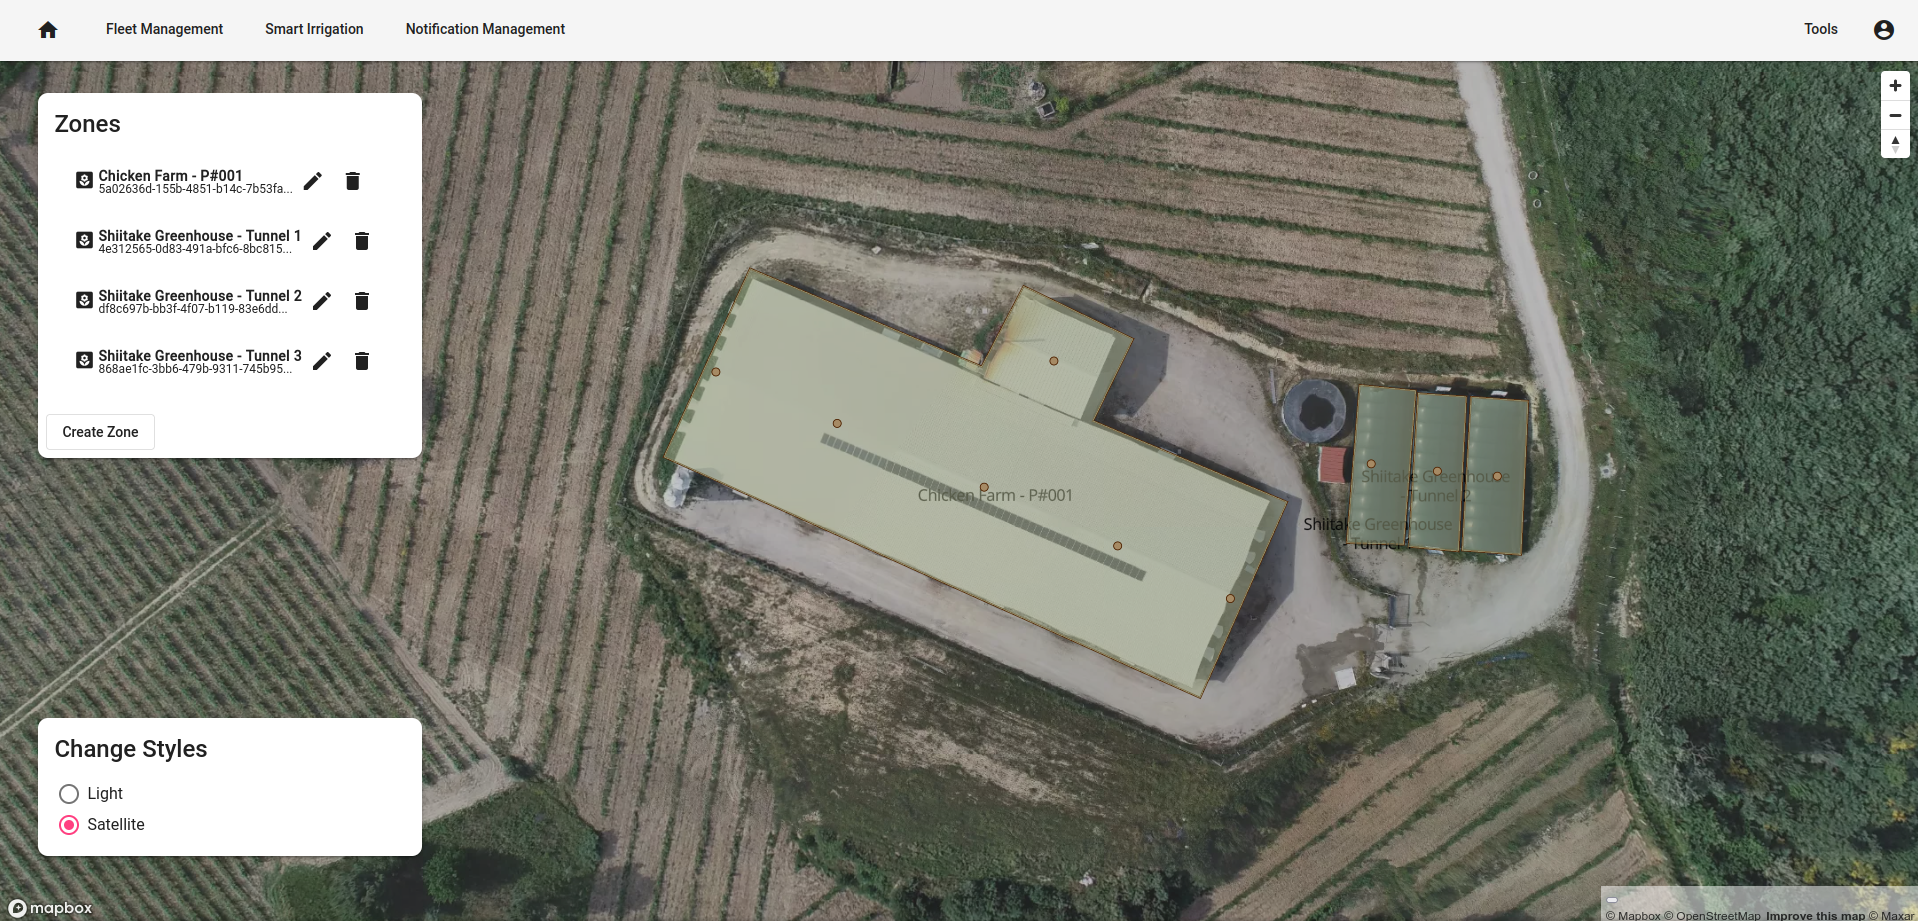
\includegraphics{assets/figures/ui/smart-irrigation-map.png}
   }
   \caption[Smart Irrigation Page - Map]{Smart Irrigation Page - Map}
   \label{fig:AppendixD2:irrigmap}
\end{figure}

\begin{figure}[H]
   \centering
   \resizebox{\columnwidth}{!}
   {
      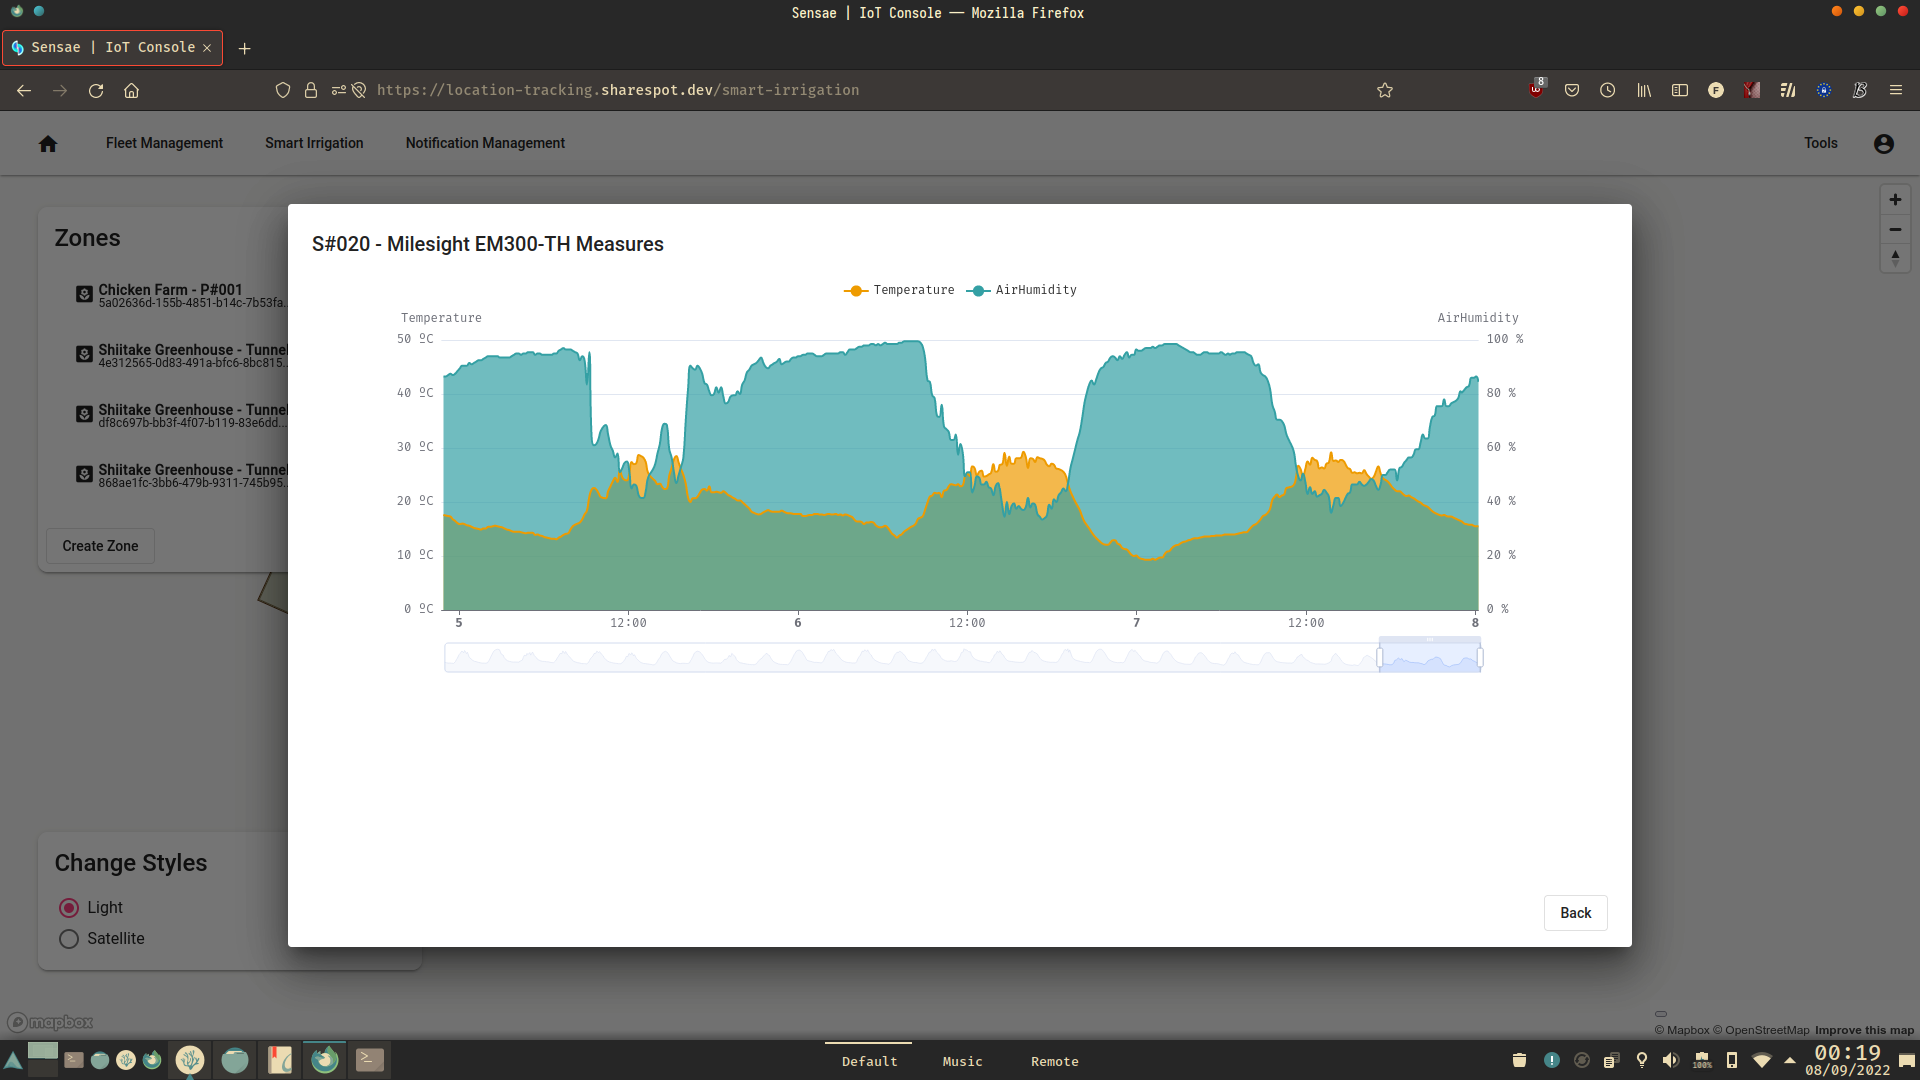
\includegraphics{assets/figures/ui/smart-irrigation-history.png}
   }
   \caption[Smart Irrigation Page - Device History]{Smart Irrigation Page - Device History}
   \label{fig:AppendixD2:irrighistory}
\end{figure}

\chapter{IoT Core Package POM}
\label{AppendixE}

\begin{lstlisting}[style=xml,basicstyle=\tiny, caption=IoT Core Package POM, label={code:AppendixE:pom}]
<project>
   <modelVersion>4.0.0</modelVersion>
   <groupId>pt.sharespot</groupId>
   <artifactId>iot-core</artifactId>
   <version>0.1.20</version>
   <name>${project.groupId}:${project.artifactId}</name>
   <description>Core library to handle the structure and behavior of messages inside Sensae Console</description>
   <url>https://sharespot.pt</url>
   <packaging>jar</packaging>
   <properties>
      <maven.compiler.source>17</maven.compiler.source>
      <maven.compiler.target>17</maven.compiler.target>
      <project.build.sourceEncoding>UTF-8</project.build.sourceEncoding>
   </properties>
   <licenses>
      <license>
         <name>The MIT License (MIT)</name>
         <url>https://mit-license.org/</url>
      </license>
   </licenses>
   <developers>
      <developer>
         <id>filipeCruz</id>
         <name>Filipe Cruz</name>
         <email>filipe.cruz@sensae.pt</email>
      </developer>
   </developers>
   <scm>
      <connection>scm:git:git@github.com:ShareSpotPT/iot-core.git</connection>
      <developerConnection>scm:git:ssh://github.com:ShareSpotPT/iot-core.git</developerConnection>
      <url>https://github.com/ShareSpotPT/iot-core/tree/master</url>
   </scm>
   <dependencies><!--omitted--></dependencies>
   <build>
      <finalName>${project.groupId}:${project.artifactId}</finalName>
      <plugins>
         <plugin>
            <groupId>org.apache.maven.plugins</groupId>
            <artifactId>maven-compiler-plugin</artifactId>
            <version>3.8.1</version>
         </plugin>
         <plugin>
            <groupId>org.apache.maven.plugins</groupId>
            <artifactId>maven-resources-plugin</artifactId>
            <version>2.5</version>
            <configuration>
               <encoding>UTF-8</encoding>
            </configuration>
         </plugin>
         <plugin>
            <groupId>org.apache.maven.plugins</groupId>
            <artifactId>maven-jar-plugin</artifactId>
            <version>3.2.0</version>
            <configuration>
               <archive>
                  <manifest>
                        <addDefaultImplementationEntries>true</addDefaultImplementationEntries>
                        <addDefaultSpecificationEntries>true</addDefaultSpecificationEntries>
                  </manifest>
               </archive>
            </configuration>
         </plugin>
         <plugin>
            <groupId>org.apache.maven.plugins</groupId>
            <artifactId>maven-source-plugin</artifactId>
            <version>3.2.1</version>
            <executions>
               <execution>
                  <id>attach-sources</id>
                  <goals>
                     <goal>jar-no-fork</goal>
                  </goals>
               </execution>
            </executions>
         </plugin>
         <plugin>
            <groupId>org.apache.maven.plugins</groupId>
            <artifactId>maven-javadoc-plugin</artifactId>
            <version>3.2.0</version>
            <executions>
               <execution>
                  <id>attach-javadocs</id>
                  <goals>
                     <goal>jar</goal>
                  </goals>
               </execution>
            </executions>
            <configuration>
               <failOnError>false</failOnError>
            </configuration>
         </plugin>
         <plugin>
            <groupId>org.apache.maven.plugins</groupId>
            <artifactId>maven-surefire-plugin</artifactId>
            <version>2.22.2</version>
         </plugin>
      </plugins>
   </build>
   <profiles>
      <profile><id>ci-cd</id>
         <build>
            <plugins>
               <plugin>
                  <groupId>org.apache.maven.plugins</groupId>
                  <artifactId>maven-gpg-plugin</artifactId>
                  <version>3.0.1</version>
                  <executions>
                     <execution>
                        <id>sign-artifacts</id>
                        <phase>verify</phase>
                        <goals>
                           <goal>sign</goal>
                        </goals>
                        <configuration>
                           <gpgArguments>
                                 <arg>--pinentry-mode</arg>
                                 <arg>loopback</arg>
                           </gpgArguments>
                        </configuration>
                     </execution>
                  </executions>
               </plugin>
            </plugins>
         </build>
      </profile>
   </profiles>
   <distributionManagement>
      <snapshotRepository><id>ossrh</id>
         <url>https://s01.oss.sonatype.org/content/repositories/snapshots</url>
      </snapshotRepository>
      <repository><id>ossrh</id>
         <url>https://s01.oss.sonatype.org/service/local/staging/deploy/maven2</url>
      </repository>
   </distributionManagement>
</project>
\end{lstlisting}

\chapter{Performance Tests Specification}
\label{AppendixF}

\begin{lstlisting}[style=javascript, caption=Smart Irrigation Performance Test Scenario Description, label={code:AppendixF:scenario1}]
//imports

export const options = {
   setupTimeout: "2m",
   scenarios: {
      subscribe: {
      executor: "shared-iterations",
      startTime: "0s",
      vus: 1,
      iterations: 1,
      maxDuration: "3m",
      exec: "subscribe",
   },
      ingestion: {
      executor: "per-vu-iterations",
      vus: 100,
      iterations: 100,
      startTime: "5s",
      exec: "ingestion",
      maxDuration: "3m",
   },
      consumption: {
      executor: "shared-iterations",
      startTime: "3m",
      vus: 1,
      iterations: 1,
      maxDuration: "10s",
      exec: "consumption",
      },
   },
};

const timeLapseTrend = new Trend("time_lapse");

const sampleSize = new SharedArray("sampleSize", function () {
   const sampleSize = [];
   sampleSize.push(options.scenarios.ingestion.vus * 
      options.scenarios.ingestion.iterations
   );
   return sampleSize;
});

const dataIds = new SharedArray("dataIds", function () {
   const dataIds = [];
   const numberOfDataUnits = options.scenarios.ingestion.vus *
      (options.scenarios.ingestion.iterations + 2);
   for (let index = 0; index < numberOfDataUnits; index++)
      dataIds.push(randomId());
   return dataIds;
});

const data = new SharedArray("data", function () {
   const data = [];
   const total = options.scenarios.ingestion.vus + 2;
   for (let index = 0; index < total; index++)
      data.push(createDevice("em300th", index, true));
   return data;
});

export function subscribe() {
   const res = http.post(`http://${__ENV.SENSAE_INSTANCE_IP}:8086/graphql`, anonymousLoginQuery, {
      headers: { "Content-Type": "application/json" },
   });

   let received = [];
   ws.connect(
      `ws://${__ENV.SENSAE_INSTANCE_IP}:8801/subscriptions`,
      {
         headers: {
            "Sec-WebSocket-Protocol": "graphql-transport-ws",
         },
      },
      (socket) => {
         socket.on("message", (msg) => {
            const message = JSON.parse(msg);
            if (message.type == "next") {
               timeLapseTrend.add(new Date().getTime() -
                  message.payload.data.data.reportedAt
               );
               received.push(message.payload.data.data.dataId);
               if (received.length === sampleSize[0]) 
                  closeSocket(socket, received);
            }
         });
         socket.on("open", () => {
            socket.send(initSubscription());
            socket.send(
               createSubscription(subscribeToLiveDataQuery, {
                  filters: createLiveDataFilters(data),
                  Authorization:
                     "Bearer " + JSON.parse(res.body).data.anonymous.token,
                  })
            );
         });
         socket.setTimeout(() => 
            closeSocket(socket, received), 300000);
      }
   );
}

export function closeSocket(socket, received) {
   check(received, { "data units were received":
      (rec) => rec.length === sampleSize[0],
   });
   received.forEach((dataId) => {
      check(dataId, {
         "data units was sent": (id) => dataIds.includes(id),
      });
   });
   socket.close();
}

export function ingestion() {
   const vu = exec.vu.idInTest - 1; //vus start at 1, arrays at 0;
   const device = data[vu];
   const id = dataIds[vu + (data.length - 2) *
      exec.vu.iterationInScenario];

   sleep(device.interval);
   const res = http.post(
      `https://${__ENV.SENSAE_INSTANCE_IP}:8443/sensor-data/${device.channel}/${device.data_type}/${device.device_type}`,
      randomBody(id, device),
      {
         headers: {
            Authorization: `${__ENV.SENSAE_DATA_AUTH_KEY}`,
            "Content-Type": "application/json",
         },
      }
   );
   check(res, { "status was 202": (r) => r.status === 202 });
}

export function consumption() {
   var numberEntries = countSmartIrrigationMeasuresEntries();
   check(numberEntries, {
      "data units were all stored": (res) => res === sampleSize[0],
   });
}

export function setup() {
   initSmartIrrigationDatabase();
   data.forEach(insertDevice);
   data.forEach(moveDeviceToPublicDomain);
   givePermissionsToPublicDomain();
   createEM300THProcessor();
   createEM300THDecoder();
}

export function teardown() {
   clearDevices();
   clearProcessors();
   clearDecoders();
   clearDomainsDevicesTenants();
   resetIdentity();
   clearIrrigationData();
}   
\end{lstlisting}

\chapter{Performance Tests Analysis}
\label{AppendixG}

\begin{lstlisting}[style=Java,basicstyle=\tiny, caption=Analysis Script, label={code:AppendixG:script}]
## Import Libraries

prepare <- function(path) {
  data <- read.csv(path)
  data <- data[data$metric_name == 'time_lapse',]
  data <- data[c('timestamp', 'metric_value', 'extra_tags')]
  data$received <- data$timestamp - min(data$timestamp)
  data$metric_value <- data$metric_value / 1000
  data$sent_timestamp <- data$timestamp - data$metric_value
  data$sent <- data$sent_timestamp - min(data$sent_timestamp)
  data$iteration <- str_replace(data$extra_tags,'iteration=' ,'')
  return(data)
}

create <- function(dataframe, xParam) {
  ggplot(data=dataframe, mapping=aes(x=.data[[xParam]], y=metric_value, col=iteration, label="")) + 
    geom_point(alpha = 1, stat = "unique") +
    theme(legend.position = c(.9, .45)) +
    xlab(paste("time data unit was", xParam, "(seconds)")) +
    ylab("time taken to process data unit (seconds)")
}

outputTex <- function(pdot, path, xParam) {
  tikz(file = path, width = 5, height = 3.3)
  print(pdot)
  dev.off()
}

process <- function(path) {
  data <- prepare(paste(path,'data.csv', sep = "/"))
  pdot_sent <- create(data, "sent")
  pdot_received <- create(data, "received")
  outputTex(pdot_sent, paste(path, 'data_sent.tex', sep="/"))
  outputTex(pdot_received, paste(path, 'data_received.tex', sep="/"))
}

processScenario <- function(path) {
  scenario <- list.dirs(path)
  scenario <- scenario[-1]
  for (i in scenario) {
    process(i)
  }
}

processAll <- function() {
  processScenario('scenario1')
  processScenario('scenario2')
  processScenario('scenario3')
}

setwd("/home/user/iot-project/project/k6/results")

processAll()
\end{lstlisting}

\chapter{Contexts - TODO}
\label{AppendixH}

\begin{landscape}
    \begin{figure}[H]
       \centering
    \resizebox{\columnwidth}{!}
    {      
       \input{assets/diagrams/design/architectural/level2/logical/contexts.latex}
    }
    \caption[Sensae Console - Context Level - Logical View Diagram]{Sensae Console - Context Level - Logical View Diagram}
       \label{fig:AppendixH:contexts}
    \end{figure}
\end{landscape}

\begin{landscape}
    \begin{figure}[H]
       \centering
    \resizebox{\columnwidth}{!}
    {      
       \input{assets/diagrams/design/architectural/level2/logical/contexts-v2.latex}
    }
    \caption[Sensae Console - Context Level V2 - Logical View Diagram]{Sensae Console - Context Level V2 - Logical View Diagram}
       \label{fig:AppendixH:contextsv2}
    \end{figure}
\end{landscape}

\begin{figure}[H]
    \centering
    \resizebox{\columnwidth}{!}
    {      
        \input{assets/diagrams/design/architectural/level2/logical/services-contexts.latex}
    }
    \caption[External Services - Context Level - Logical View Diagram]{External Services - Context Level - Logical View Diagram}
    \label{fig:AppendixH:servicecontexts}
\end{figure}

\begin{figure}[H]
    \centering
    \resizebox{\columnwidth}{!}
        {      
        \input{assets/diagrams/design/architectural/level2/logical/data-decoder-context.latex}
        }
    \caption[Data Decoder - Container Level - Logical View Diagram]{Data Decoder - Container Level - Logical View Diagram}
    \label{fig:AppendixH:decoder}
\end{figure}

\begin{figure}[H]
    \centering
    \resizebox{\columnwidth}{!}
        {      
        \input{assets/diagrams/design/architectural/level2/logical/data-processor-context.latex}
        }
    \caption[Data Processor - Container Level - Logical View Diagram]{Data Processor - Container Level - Logical View Diagram}
    \label{fig:AppendixH:processor}
\end{figure}

\begin{figure}[H]
    \centering
    \resizebox{\columnwidth}{!}
        {      
        \input{assets/diagrams/design/architectural/level2/logical/device-management-context.latex}
        }
    \caption[Device Management - Container Level - Logical View Diagram]{Device Management - Container Level - Logical View Diagram}
    \label{fig:AppendixH:device}
\end{figure}

\begin{figure}[H]
    \centering
    \resizebox{\columnwidth}{!}
        {      
        \input{assets/diagrams/design/architectural/level2/logical/identity-management-context.latex}
        }
    \caption[Identity Management - Container Level - Logical View Diagram]{Identity Management - Container Level - Logical View Diagram}
    \label{fig:AppendixH:identity}
\end{figure}

\begin{figure}[H]
    \centering
    \resizebox{\columnwidth}{!}
        {      
        \input{assets/diagrams/design/architectural/level2/logical/rule-management-context.latex}
        }
    \caption[Rule Management - Container Level - Logical View Diagram]{Rule Management - Container Level - Logical View Diagram}
    \label{fig:AppendixH:rule}
\end{figure}

\begin{figure}[H]
    \centering
    \resizebox{\columnwidth}{!}
        {      
        \input{assets/diagrams/design/architectural/level2/logical/fleet-management-context.latex}
        }
    \caption[Fleet Management - Container Level - Logical View Diagram]{Fleet Management - Container Level - Logical View Diagram}
    \label{fig:AppendixH:fleet}
\end{figure}

\begin{figure}[H]
    \centering
    \resizebox{\columnwidth}{!}
        {      
        \input{assets/diagrams/design/architectural/level2/logical/notification-management-context.latex}
        }
    \caption[Notification Management - Container Level - Logical View Diagram]{Notification Management - Container Level - Logical View Diagram}
    \label{fig:AppendixH:notification}
\end{figure}

\begin{figure}[H]
    \centering
    \resizebox{\columnwidth}{!}
        {      
        \input{assets/diagrams/design/architectural/level2/logical/smart-irrigation-context.latex}
        }
    \caption[Smart Irrigation Management - Container Level - Logical View Diagram]{Smart Irrigation Management - Container Level - Logical View Diagram}
    \label{fig:AppendixH:irrigation}
\end{figure}


%----------------------------------------------------------------------------------------

\end{document}
